%% NYU PhD thesis format. Created by José Koiller 2007--2008.
%% Updated by Anshul Vikram Pandey with new design guidelines. 2017-2018

%% Use the first of the following lines during production to
%% easily spot "overfull boxes" in the output. Use the second
%% line for the final version.
\documentclass[12pt,draft,letterpaper]{report}
% \documentclass[12pt,letterpaper]{report}
% \documentclass[12pt]{article}

%% Replace the title, name, advisor name, graduation date and dedication below with
%% your own. Graduation months must be January, May or September.
%WILLING STATELESSNESS: THREE ESSAYS ON THE POLITICAL ECONOMY OF LOCAL GOVERNMENTS IN ONGOING CRIMINAL WARS''
\newcommand{\thesistitle}{ESSAYS ON THE POLITICAL ECONOMY OF LOCAL GOVERNMENTS IN ONGOING CRIMINAL WARS}
\newcommand{\thesisauthor}{Rafael J. Ch Duran}
\newcommand{\thesisadvisor}{Pablo Querubin Borrero}
\newcommand{\graddate}{June 2021} % like January XX, May 20XX, September 20XX

%% If you do not want a dedication, scroll down and comment out
%% the appropriate lines in this file.
\newcommand{\thesisdedication}{A mis tres princesas, Mamá, Areli y Lala (juntitos para siempre)}

%% The following makes chapters and sections, but not subsections,
%% appear in the TOC (table of contents). Increase to 2 or 3 to
%% make subsections or subsubsections appear, respectively. It seems
%% to be usual to use the "1" setting, however.
\setcounter{tocdepth}{1}

%% Sectional units up to subsubsections are numbered. To number
%% subsections, but not subsubsections, decrease this counter to 2.
\setcounter{secnumdepth}{3}

% Setting a gap between page number and text block


%% Page layout (customized to letter paper and NYU requirements):
\setlength{\oddsidemargin}{.6in}
\setlength{\textwidth}{5.8in}
\setlength{\topmargin}{0.5in}
\setlength{\headheight}{0in}
\setlength{\headsep}{0in}
\setlength{\textheight}{8.3in}
\setlength{\footskip}{.5in}

%% Use the following commands, if desired, during production.
%% Comment them out for final version.
%\usepackage{layout} % defines the \layout command, see below
%\setlength{\hoffset}{-.75in} % creates a large right margin for notes and \showlabels

      


%%%%%%

%% Controls spacing between lines (\doublespacing, \onehalfspacing, etc.):
\usepackage{setspace}

%
%% \usepackage{amsmath}
%% \usepackage{amssymb}
\usepackage{xspace}
\usepackage{algorithmic}
\usepackage{algorithm}
\usepackage{microtype}
\usepackage{subfigure}
\usepackage{color}
\usepackage{url}
\usepackage{lipsum}
\usepackage{fancyhdr}
% \newfloat{algorithm}{t}{lop}

\pagestyle{fancy}
\fancyhf{}
\renewcommand{\headrulewidth}{0pt}
\fancyhead[LE]{}
\fancyhead[RO]{}
\fancyhead[RE]{}
\fancyhead[LO]{}
\fancyfoot[C]{}
\rhead{\thepage}

\fancypagestyle{plain}{%
\fancyhf{}
\rhead{\thepage}
}

\setlength{\headheight}{20pt} 

%% Use the line below for official NYU version, which requires
%% double line spacing. For all other uses, this is unnecessary,
%% so the line can be commented out.
\onehalfspacing % requires package setspace, invoked above

%% Each of the following lines defines the \com command, which produces
%% a comment (notes for yourself, for instance) in the output file.
%% Example:    \com{this will appear as a comment in the output}
%% Choose (uncomment) only one of the three forms:
%\newcommand{\com}[1]{[/// {#1} ///]}       % between [/// and ///].
\newcommand{\com}[1]{\marginpar{\tiny #1}} % as (tiny) margin notes
%\newcommand{\com}[1]{}                     % suppress all comments.

%% This inputs your auxiliary file with \usepackage's and \newcommand's:
%% It is assumed that that file is called "definitions.tex".
%%
%% Place here your \usepackage's. Some recommended packages are already included.
%%

% Graphics:
\usepackage[final]{graphicx}
%\usepackage{graphicx} % use this line instead of the above to suppress graphics in draft copies
%\usepackage{graphpap} % \defines the \graphpaper command

% Indent first line of each section:
\usepackage{indentfirst}

% Good AMS stuff:
\usepackage{amsthm} % facilities for theorem-like environments
\usepackage[tbtags]{amsmath} % a lot of good stuff!

% Fonts and symbols:
\usepackage{amsfonts}
\usepackage{amssymb}

\usepackage{xspace}
\usepackage{algorithmic}
\usepackage{algorithm}
\usepackage{microtype}
\usepackage{subfigure}
\usepackage{color}
\usepackage{todonotes}
\usepackage{url}
\newfloat{algorithm}{t}{lop}

% Formatting tools:
%\usepackage{relsize} % relative font size selection, provides commands \textsmalle, \textlarger
%\usepackage{xspace} % gentle spacing in macros, such as \newcommand{\acims}{\textsc{acim}s\xspace}

% Page formatting utility:
\usepackage{geometry}
\usepackage{multirow}
\usepackage{listings}
%
\usepackage[round,authoryear]{natbib}
\usepackage[all,cmtip]{xy}
\usepackage[colorlinks=true,citecolor=blue,urlcolor=blue, filecolor=blue,pdfpagemode=UseNone,pdfstartview=FitH, final]{hyperref}
%\usepackage[breaklinks=true,a4paper=true,pagebackref=true]{hyperref}
\usepackage{tocloft}
\newcommand{\Color}[1]{\hypersetup{linkcolor=#1}\color{#1}}
\renewcommand{\cftchapfont}{\Color{black}\large\bfseries}
\renewcommand{\cftsecfont}{\Color{black}}
\renewcommand{\cftsubsecfont}{\Color{black}}
\renewcommand{\cftsubsubsecfont}{\Color{black}}
\renewcommand{\cftchappagefont}{\Color{black}}
\renewcommand{\cftsecpagefont}{\Color{black}}
\renewcommand{\cftsubsecpagefont}{\Color{black}}
\renewcommand{\cftsubsubsecpagefont}{\Color{black}}
\renewcommand{\cftsecleader}{\Color{black}\cftdotfill{\cftsecdotsep}}
\renewcommand{\cftsubsecleader}{\Color{black}\cftdotfill{\cftsubsecdotsep}}
\renewcommand{\cftsubsubsecleader}{\Color{black}\cftdotfill{\cftsubsubsecdotsep}}
\renewcommand{\cftchapleader}{\large\bfseries\color{black}\cftdotfill{\cftdotsep}}
\renewcommand{\cftchappagefont}{\large\bfseries}
%\usepackage{hyperref}
%\hypersetup{
 %   colorlinks=true,
  %  linkcolor=blue,
   % filecolor=blue,
%    urlcolor=blue,
 %    citecolor=blue
 % }

%%
%% Place here your \newcommand's and \renewcommand's. Some examples already included.
%%
%\newcommand{\acims}{\textsc{acim}s\xspace}
\newcommand{\Mspace}        {{\mathbb M}}
\newcommand{\Rspace}        {{\mathbb R}}
\newcommand{\Cspace}        {{\mathbb C}}

\newcommand{\Mo}        {{\hat M}}
\newcommand{\Ms}        {{\tilde M}}
\newcommand{\Do}          {{\hat D}}
\newcommand{\Ds}        {{\tilde D}}
\newcommand{\doo}          {{\hat d}}
\newcommand{\dss}        {{\tilde d}}
\newcommand{\w}        {{\mathbf w}}

% general
\newcommand{\ie}{i.e.}
\newcommand{\eg}{e.g.}
\newcommand{\reffig}[1]{{Figure~\ref{#1}}}
\newcommand{\refchap}[1]{{Chapter~\ref{#1}}}
\newcommand{\refsec}[1]{{Section~\ref{#1}}}
\newcommand{\reftab}[1]{{Table~\ref{#1}}}
\newcommand{\refapp}[1]{{Appendix~\ref{#1}}}
\newcommand{\refeq}[1]{{Equation~\ref{#1}}}
\newcommand{\refalg}[1]{{Algorithm~\ref{#1}}}
\newcommand{\myparagraph}[1]{\noindent \textbf{#1}}
\newcommand{\highlight}[1]{{\color{black}#1}}


%%%%RAFA PACKAGES
\usepackage[font=bf, justification=centering]{caption}
\DeclareUnicodeCharacter{00A0}{'}
\usepackage{longtable}    
\usepackage{lscape}
\usepackage{booktabs}
%\usepackage[colorlinks=true,citecolor=blue,urlcolor=blue,pdfpagemode=UseNone,pdfstartview=FitH]{hyperref}

%%
%% Place here your \newtheorem's:
%%

%% Some examples commented out below. Create your own or use these...
%%%%%%%%%\swapnumbers % this makes the numbers appear before the statement name.
%\theoremstyle{plain}
%\newtheorem{thm}{Theorem}[chapter]
%\newtheorem{prop}[thm]{Proposition}
%\newtheorem{lemma}[thm]{Lemma}
%\newtheorem{cor}[thm]{Corollary}

%\theoremstyle{definition}
%\newtheorem{define}{Definition}[chapter]

%\theoremstyle{remark}
%\newtheorem*{rmk*}{Remark}
%\newtheorem*{rmks*}{Remarks}

%% This defines the "proo" environment, which is the same as proof, but
%% with "Proof:" instead of "Proof.". I prefer the former.
%\newenvironment{proo}{\begin{proof}[Proof:]}{\end{proof}}


%% Cross-referencing utilities. Use one or the other--whichever you prefer--
%% but comment out both lines for final version.
%\usepackage{showlabels}
%\usepackage{showkeys}
% \pagestyle{headings}

\begin{document}
%% Produces a test "layout" page, for "debugging" purposes only.
%% Comment out for final version.
%\layout % requires package layout (see above, on this same file)
%% Sets page numbering to "roman style" i, ii, iii, iv, etc:

%%%%%% Cover page %%%%%%%%%%%
%% Sets page numbering to "roman style" i, ii, iii, iv, etc:
\pagenumbering{roman}
\thispagestyle{empty}
\begin{center}
{\bfseries 
  {\large\thesistitle}
  \vspace{1in}
  
 {\large {\bf DISSERTATION}}\\
  \vspace{.3in}
  
  \begin{doublespace}
  {\large  
  Submitted in Partial Fulfillment of\\
  % \vspace{.1in}
  the Requirements for\\
  % \vspace{.1in}
  the Degree of\\}
  \end{doublespace}
  \vspace{.3in}
  
  {\large DOCTOR OF PHILOSOPHY \\ (Political Science)}\\
  \vspace{.5in}
  
  at the \\
  \vspace{.2in}
  
  {\large
  NEW YORK UNIVERSITY\\
  \vspace{-0.05in}
  GRADUATE SCHOOL OF ARTS AND SCIENCE\\
  }
  \vspace{.2in}
  
  by
  \vspace{.5in}

  {\large\thesisauthor}
  \vspace{.5in}
  % \vfill

  {\large\graddate}
}

\end{center}

\newpage

%%%%%% Title page %%%%%%%%%%%
%
\setcounter{page}{1}
%% No numbering in the title page:
\thispagestyle{empty}
%
\begin{center}
{\bfseries 
  {\large\thesistitle}
  \vspace{.2in}
  
  DISSERTATION\\
  \vspace{.2in}
  
  \begin{doublespace}
  Submitted in Partial Fulfillment of\\
  % \vspace{.1in}
  the Requirements for\\
  % \vspace{.1in}
  the Degree of\\
  \end{doublespace}
  \vspace{.2in}
  
  DOCTOR OF PHILOSOPHY  (Political Science)\\
  \vspace{.2in}
  
  at the \\
  \vspace{.1in}
  
  {\large
  NEW YORK UNIVERSITY\\
  \vspace{-0.05in}
  GRADUATE SCHOOL OF ARTS AND SCIENCE\\
  }
  \vspace{.1in}
  
  by
  \vspace{.15in}

  \thesisauthor
  \vspace{.15in}
  % \vfill

  \graddate
}

\end{center}
% \vfill

\vspace{0.2in}

\noindent
\makebox[\textwidth]{\hfill\makebox[2.5in]{Approved: \hfill}}
\vspace{0.1in}

\noindent
\makebox[\textwidth]{\hfill\makebox[2.5in]{\hrulefill}}\\
\makebox[\textwidth]{\hfill\makebox[2.5in]{\hfill Department Chair Signature\hfill}}
\vspace{0.05in}

\noindent
\makebox[\textwidth]{\hfill\makebox[2.5in]{\hrulefill}}\\
\makebox[\textwidth]{\hfill\makebox[2.5in]{\hfill Date \hfill}}

\noindent
University ID: {N16628197}\\ % Add your University ID
Net ID: \hspace{.415in} {rcd306}\\ % Add your Net ID
\break
%\newpage

%%%%%%%%%%%%%% Copyright Page %%%%%%%%%%%%%%%%%

%%%%%%%%%%%%%% Guidance Committee Signature Page %%%%%%%%%%%%%%%%%
\singlespacing
\noindent
Approved by the Guidance Committee: \\
\underline{Major}: Political Science
%\vspace{0.01in}

\noindent
\makebox[\textwidth]{\hfill\makebox[3in]{\hrulefill}}\\
\makebox[\textwidth]{\hfill\makebox[3in]{\hfill \textbf{Pablo Querubin Borrero}\hfill}}
\makebox[\textwidth]{\hfill\makebox[3in]{\hfill Associate Professor of \hfill}}
\makebox[\textwidth]{\hfill\makebox[3in]{\hfill Politics and Economics at NYU \hfill}}
\makebox[\textwidth]{\hfill\makebox[3in]{\rule[-4pt]{2in}{1pt}}}\\
\makebox[\textwidth]{\hfill\makebox[3in]{\hfill June 24, 2021 \hfill}}\\
\vspace{0.1in}
\noindent
\makebox[\textwidth]{\hfill\makebox[3in]{\hrulefill}}\\
\makebox[\textwidth]{\hfill\makebox[3in]{\hfill \textbf{Cyrus Samii}\hfill}}
\makebox[\textwidth]{\hfill\makebox[3in]{\hfill Associate Professor of \hfill}}
\makebox[\textwidth]{\hfill\makebox[3in]{\hfill Politics at NYU \hfill}}
\makebox[\textwidth]{\hfill\makebox[3in]{\rule[-4pt]{2in}{1pt}}}\\
\makebox[\textwidth]{\hfill\makebox[3in]{\hfill June 24, 2021 \hfill}}\\
\vspace{0.1in}
\noindent
\makebox[\textwidth]{\hfill\makebox[3in]{\hrulefill}}\\
\makebox[\textwidth]{\hfill\makebox[3in]{\hfill \textbf{Hye Young You}\hfill}}
\makebox[\textwidth]{\hfill\makebox[3in]{\hfill Assistant Professor of \hfill}}
\makebox[\textwidth]{\hfill\makebox[3in]{\hfill Politics at NYU \hfill}}
\makebox[\textwidth]{\hfill\makebox[3in]{\rule[-4pt]{2in}{1pt}}}\\
\makebox[\textwidth]{\hfill\makebox[3in]{\hfill June 24, 2021 \hfill}}\\
\vspace{0.1in}
\noindent
\makebox[\textwidth]{\hfill\makebox[3in]{\hrulefill}}\\
\makebox[\textwidth]{\hfill\makebox[3in]{\hfill \textbf{Tara Slough}\hfill}}
\makebox[\textwidth]{\hfill\makebox[3in]{\hfill Assistant Professor of \hfill}}
\makebox[\textwidth]{\hfill\makebox[3in]{\hfill Politics at NYU \hfill}}
\makebox[\textwidth]{\hfill\makebox[3in]{\rule[-4pt]{2in}{1pt}}}\\
\makebox[\textwidth]{\hfill\makebox[3in]{\hfill June 24, 2021 \hfill}}\\
\vspace{0.1in}
\noindent
\makebox[\textwidth]{\hfill\makebox[3in]{\hrulefill}}\\
\makebox[\textwidth]{\hfill\makebox[3in]{\hfill \textbf{Juan F. Vargas}\hfill}}
\makebox[\textwidth]{\hfill\makebox[3in]{\hfill Professor of \hfill}}
\makebox[\textwidth]{\hfill\makebox[3in]{\hfill Economics at Universidad El Rosario \hfill}}
\makebox[\textwidth]{\hfill\makebox[3in]{\rule[-4pt]{2in}{1pt}}}\\
\makebox[\textwidth]{\hfill\makebox[3in]{\hfill June 24, 2021 \hfill}}\\

\doublespacing

%%%%%%%%%%%%%% Microfilm / Publishing Page %%%%%%%%%%%%%%%%%
\break
\begin{center}
\copyright  by Rafael J. Ch Durán, 2021. All rights reserved.

%Microfilm or other copies of this dissertation are obtainable from
%\vspace{4in}

%UMI Dissertation Publishing\\
%ProQuest CSA\\
%789 E. Eisenhower Parkway\\
%P.O. Box 1346\\
%Ann Arbor, MI 48106-1346

\end{center}
\newpage

%%%%%%%%%%%%%% Vita %%%%%%%%%%%%%%%%%
\section*{Vita}
\addcontentsline{toc}{section}{Vita}
%!TEX root = thesis.tex

I’m a Ph.D. Candidate in the Politics Department at New York University. My research interests lie in Comparative Politics and Methods, and include the study of Governance, Conflict, and State Capture. I have a regional specialization in developing countries, particularly Latin America.

I received NYU’s Dean’s Dissertation Fellowship 2020-2021. My research has also been supported by organizations including the Fulbright-Garcia Robles Program, the Development Bank of Latin America (CAF), the Center for Studies in Security and Drugs (CESED) from Universidad Los Andes, among others. My scholarly work has been published in the American Political Science Review, the Journal of Urban Economics and I have been a referee for the American Political Science Review, Comparative Political Studies, and Latin American Research Review.

While in the Ph.D. program at NYU, I also served as Principal Investigator for the Latin America Development Bank´s (CAF) “Slum Observatory” Project, and worked on CAF’s leading chapter of the flagship annual Economy and Development Report 2017 on Urban Development in Latin America. In 2015 I served as a Research Assistant at the Empirical Studies of Conflict (ESOC) at Princeton University. Prior to NYU, I served as Director of the Economic and Public Security Research Division at the Center of Research for Development, A.C. (CIDAC), and as a Visiting Professor at the Political Science Department of the Instituto Tecnológico Autónomo de México (ITAM) where I thought Political Methodology. I received my BA in Economics from ITAM with the highest distinction. 

\newpage



%%%%%%%%%%%%%% Ackknowlegment %%%%%%%%%%%%%%%%%
%% Comment out the following lines if you do not want to acknowledge
%% anyone's help...
\section*{Acknowledgements}
\addcontentsline{toc}{section}{Acknowledgements}
%!TEX root = thesis.tex

%% Write your acknowledgements in this file. If you do not want to acknowledge anyone,
%% you can delete this file and comment out the corresponding part in the "thesis.tex"
%% file.


This dissertation is the result of multiple years of work and the involvement of many people. There are no words to express the gratitude and appreciation to every single person that supported me throughout the last 7 years at NYU. Thanks to all of you, I finish this stage in life with a heart filled with joy and hope for things to come. 

First and foremost, I want to thank my dissertation committee. Pablo Querubin, thank you for believing in me since we first met, for giving me the opportunity to teach side-by-side with you for five years, for always being patient with me, for spending countless hours to talk about my research and even job opportunities, for always doing so with a big smile. Thank you for your advice inside and outside the classroom, for leading me to new research opportunities, for pushing my research, for being my mentor and friend. I will never forget the words you gave to the Latin American Politics class in the last lecture of Spring of 2017: you spoke of how the class revolved around portraying the faults of Latin America but that students should not loose sight of the beauties of the region, and the promise of hope for it. Your love for Latin America is something I will carry on for the rest of my life. Cyrus Samii, there is no way I can express how much I thank you for all your support these years. There were times in the Ph.D. program where I thought I couldn't make it but it was your advice and guidance throughout these years that help me build confidence in my research. I will never forget the days spend in Morocco, your help to meet new faculty members, your methodological teaching, your mentoring and support. Hye Young You, the first time I met you, you had read all of my work in such a thorough way that left me amazed. Your insights and clarity have been extremely helpful, and much of what I could do in this dissertation was thanks to those meetings with you. If the kindness and patience you have showed to me was present in every faculty member, academia would be the best of places in the world. Tara Slough, as I have told you before, every time I see you participate in a seminar, deliver comments to students or in conferences, and when you have spoken directly to my research you have always provided the best of feedback. I have long admired your research and work ethic. Begin honest, I wish I could be like you, and I'm so happy to have you as part of my committee. Juan Vargas, mi mentor y mi amigo, if there is someone to truly thank throughout all these years is you. Since the Summer of 2015 you opened your arms to me as a collegue, and few days after as friend for life. There is no one I have learned from as you, who truly built up my foundations as a researcher, who opened up research opportunities to me that I would have never dreamed about. 

I also want to thank the faculty members at NYU and Princeton University. Neal Beck, there is no man in academia like you, there is no one that loves students as you do. It is becasue of you that a boy in a Masters program with hopes of joining a Ph.D. program achieved his dream as is now about to finish it. I will be eternally grateful for your support and friendship. Jake Shapiro, I met you at the end of my first year at the Masters at NYU. Since then my life changed and I couldn't even imagine everything that happened since, and much of it was due to your mentoring, support, and friendship. You are a dreambuilder, and I have achieved many of my dreams by being under your wing. I'm truly thankful to you and excited for the work to come in the following years. Leonard Wantchekon, thank you for sharing some of your passion for research and how to better the world we are living in. Your trust in me and all the research opportunities you have shared with me cannot be repaid.

Thank you for all the faculty members at NYU that shared their knowledge and advice during my doctoral studies. Thank you Dimitri Landa, Peter Rosendorff, Shanker Satyanath, Nicole Simonelli,  Amanda Kennard, Tiberiu Dragu, Mike Gilligan, David Stasavage, and Julia Payson.  

God has given me the best friends: I am truly the happiest man of the world because of you. Gordos, Gabriel y Gizeh, mis amigos del alma, los tres mosqueteros hasta el final, verdaderamente me han enseñado que el hierro con hierro se afila. Alan, el hermano que nunca tuve y que me ha acompañado hasta este día. Si en alguien dejara mi vida sería en tus manos. Así como tus logros son mis logros, espero \'este sea uno tuyo pues no pude haberlo alcanzado sin tu amistad. Andresiño -my fish!- y Juanda, mis dos hermanos de otros padres, dos regalos que Dios me dió de pura gracia y que serán mi familia por siempre. Nick, I never thought to find a friend like you in the States, and to admire a man the way I admire you. You are one of God's best gifts I have in my life. I have missed you since you left NYC. Prabin, your heart is the biggest of all, and your friendship a true gift. To both of you, Nick and Prabin, I couldn´t have done the Ph.D. without you, you were the greatest support, and the truest of friends. Reed, I wish we could have met earlier in the progam but I thank God for that trip to China, for the endless talks we have had since, for your friendship, your guidance and mentoring. We are brothers for life. To all my friends at NYU, thank you: Will, Antonella, Mateo, Mariana, Dongil, Abraham, Felipe, Martin, Patrick, Arina, Maria, Anne, Giacomo, Athena, Rajeshwari, Lucia, Ye, and Stephanie.

To my friends in NYC, thank you for being present throughout these years, for all your prayers and support. Rich, my dear friend and brother, you have been and advisor and the best of friends. Truly, you have showed me that there is a friend that is closer than a brother. Jing, there is no day that I miss you in NY. God blessed me with your life since we met. To all the members of the Stuy CG and Redeemer, Fei Mei, Sam, Melody, Miguelo, Emilia, Diane, Becks, Audrey, and many, many more. To all of you and even the ones I don't name, thank you for your frienship and your love. You are my NYC family, and there is no better family than you all. 

To my students from the IR Honors, Latin American Politics, and Political Economy of Development classes at NYU, thank you. Back when I was living in Mexico and before coming to the States I had a dream of becoming an advisor to kings and queens. For years I thought I would achieve that by taking a job in public office. You, however, thought me that by teaching I was already fulfilling the biggest dream in my heart. You, my kings and queens, are my joy and glory. 

Finally, and most importantly, I'm grateful to my family. Mamá eres a quien más admiro en el mundo y cuyo amor me sostuvo todos estos años: mi gran consejera y mi gran amiga. Arela y Lala, mis amores, mis hermanitas hermosas que con su amor me apoyaron día tras día, y me hacen querer ser mejor cada día. A las tres sepan que mis sueños cumplidos son suyos, mis logros sus logros, mi honor su honor, pues no hay nada que que hubiera logrado sin ustedes. Su amor es mi motor y el regalo más grande de Dios en esta vida. Esta disertación se las dedico a ustedes. Las amo.

God, I have fought the good fight, I have finished the race, I have kept the faith. You have lifted my head up high, you have sustained me and loved me like nobody has. My life is yours, this degree is yours, and to you, who is able to do immesurably more than all we ask or imagine, to you God be the glory forever and ever. 

\noindent
\makebox[\textwidth]{\hfill\makebox[3in]{\hfill Rafael J. Ch Duran\hfill}}
\makebox[\textwidth]{\hfill\makebox[3in]{\hfill\graddate\hfill}}


\newpage

%%%%%%%%%%%%%% Dedication Page %%%%%%%%%%%%%%%%%
%% Comment out the following lines if you do not want to dedicate
%% this to anyone...
\vspace*{\fill}
\begin{center}
  \thesisdedication%\addcontentsline{toc}{section}{Dedication}
\end{center}
\vfill
\newpage


%%%%%%%%%%%%%% Abstract %%%%%%%%%%%%%%%%%
\section*{}
\begin{center}
{\bfseries 
  %{\large\thesistitle}
  \vspace{.25in}  
  {\bf ABSTRACT}\\
  \vspace{.25in}
  {\bf \thesistitle}\\  
  \vspace{.25in}
  {\bf by}\\  
  \vspace{.5in}
  {\bf \thesisauthor}\\
  \vspace{.5in}
  {\bf Advisor: Prof. \thesisadvisor, Ph.D.}\\
  \vspace{.25in}
  {\bf Submitted in Partial Fulfillment of the Requirements for}\\
  {\bf the Degree of Doctor of Philosophy (Political Science)}\\
  \vspace{.25in}
  {\bf \graddate}  
  \vspace{.25in}
}
\end{center}
\addcontentsline{toc}{section}{Abstract}
%!TEX root = thesis.tex

This dissertation studies what prevents (or fosters) would-be contemporary nation-builders from building the nation and solidifying the state when challenged by criminal wars. Focusing on Mexico and Colombia -two states rampaged by ongoing criminal wars-, I study the incentives of local governments electoral incentives (Chapter 1 and 2), and the way in which non-state armed groups capture them and transform local institutions to their preferences (Chapter 3). 

The first chapter titled ``Reelection Backfire: How Reelection Concerns Affect the Delegation of Public Security Policy in Mexico'' studies the effect of reelection incentives of mayors on the delegation of security policy to governors in Mexico. It is no easy task for local governments to combat organized crime and hold the monopoly of violence. Faced by resource, expertise, or information constraints, or in the presence of large spillovers, mayors may choose to delegate security policy to more efficient agents like the governor or the president. However, by doing so mayors loose the use of security policy for electoral purposes: they cannot longer claim competence and willingness to fight crime or be responsive to citizens demands. A clear tradeoff between efficiency and electoral incentives arises. This paper studies the effect of mayors' reelection incentives on the delegation of security policy to the governor in a country overwhelmed by criminal wars, Mexico. To do so, I leverage the staggered implementation of an electoral reform that introduced reelection for mayors from 2014 to 2022. I find that mayors up for reelection decrease the delegation of public security to the governor of their state relative to term-limited mayors. By taking charge of policy, mayors facing reelection differentiate themselves from other political actors believing this would increase their reelection chances. However, no evidence is found that mayors increase their effort to fight crime and address citizens security concerns. The consequence of not delegating to more efficient actors, however, is an increase in violence. This paper suggests that delegation is not only a policy decision but an electoral one, and that reelection incentives may lead incumbents to differentiate themselves by taking charge of public policy at the expense of efficiency.   

The second chapter titled ``Love the Candidate but Hate his Party: The Asymmetric Effects of Reelection Incentives on Partisan and Personal Incumbency Returns in Mexico'' studies incumbency returns to office in local governments. A large literature has studied the electoral returns to incumbency. However, the estimated incumbency returns in the majority of studies confound the returns to the incumbent party and politician. As a result we may hold a misguided picture of the relationship between parties and their members, citizens valuation of the electoral system, and the existent electoral accountability. This paper opens up the black box of incumbency by disentangling the personal and partisan incumbency advantages. To do so, I use a difference-in-discontinuity of close elections design in Mexico that exploits the staggered implementation of an electoral reform that introduced reelection for mayors from 2014 to 2022. Term limit elections allow us to identify a partisan advantage since the politician cannot run for office again but his party can. Elections with candidates up for reelection identify both the partisan and personal incumbency returns.  The difference between this two quantities -or the difference-in-discontinuity estimator- identifies the personal from the partisan effect. The main result shows that incumbent politicians up for reelection enjoyed and electoral \emph{advantage}. Contrastingly, incumbent parties in term limit races suffer from an incumbency \emph{disadvantage}. The research design allows to solve several methodological issues of past studies that have tried to disentangle the partisan from the personal effect, primarily rule out potential pretrends of term limit and non-term limit races, as well as concerns on selection coming from the ability and experience of candidates. Overall, the results suggest the personal advantage to be a driving force of incumbency returns, and how  reelection may lead to party dealignment in party-centered systems like Mexico. 

Lastly, the third chapter titled ``Endogenous taxation in ongoing internal conflict: The case of Colombia'' studies how non-state armed groups capture municipalities and transform local institutions according to their preferences. Recent empirical evidence suggests an ambiguous relationship between internal conflicts, state capacity and tax performance. In theory, internal conflict should create strong incentives for governments to develop the fiscal capacity necessary to defeat rivals. In this chapter we argue that one reason that this does not occur is because internal conflict enables groups with {\it{de facto}} power to capture local fiscal and property rights institutions. We test this mechanism in Colombia using data on tax performance and property rights institutions at the municipal level. Municipalities affected by internal conflict have tax institutions consistent with the preferences of the parties dominating local violence. Those suffering more right-wing violence feature more land formalization and higher property tax revenues. Municipalities with substantial left-wing guerrilla violence collect less tax revenue and witness less land formalization. Our findings provide systematic evidence that internal armed conflict helps interest groups capture municipal institutions for their own private benefit, impeding state-building.


\newpage

%%%% Table of Contents %%%%%%%%%%%%
\tableofcontents
% \clearpage
% \pagestyle{headings}

%%%%% List of Figures %%%%%%%%%%%%%
%% Comment out the following two lines if your thesis does not
%% contain any figures. The list of figures contains only
%% those figures included withing the "figure" environment.
\listoffigures\addcontentsline{toc}{section}{\listfigurename}
\newpage

%%%%% List of Tables %%%%%%%%%%%%%
%% Comment out the following two lines if your thesis does not
%% contain any tables. The list of tables contains only
%% those tables included withing the "table" environment.
\listoftables\addcontentsline{toc}{section}{\listtablename}
\newpage

%%%%% Body of thesis starts %%%%%%%%%%%%
\pagenumbering{arabic} % switches page numbering to arabic: 1, 2, 3, etc.

%% Introduction. If your thesis has no introduction, or chapter 1 is
%% meant to be the introduction, then comment out the lines below.
%% \section*{Introduction}\addcontentsline{toc}{section}{Introduction}
%\input{intro}

%%If your thesis has different "Parts", use commands such as the following:

\section{Introduction}
      
                    
Normatively, efficiency and equity considerations should determine which level of government takes charge of policy and public good delivery \citep{oates_1972, Musgrave_1959, Musgrave_1983, gramlich_1977}. In some cases, however, certain levels of government may hold the responsibility of policymaking despite being the least efficient to do so due to constraints on resources \citep{Moravcsik_2000}, expertise or information \citep{Rodrick_1996} or the existence of spillovers \citep{oates_1972,  Besley_case_1995}. This is the case of the monopoly of violence in conflict settings where subnational units might not be able to fight non-state armed groups: they may be more prone to capture, coercion and strife \citep{chacon_2018}, and their fight against crime might only create a ``balloon effect’’ where criminal organizations simply move to nearby localities where crime is less well clamped down \citep{shirk_wallman_2015}. Unable to deliver security policy efficiently, subnational governments may choose to delegate it to upper-level governments who can pool resources, gather better information, develop economies of scale and specialize \citep{Hawkins_etal_2006}, and combat crime more efficiently. By delegating, however, incumbents lose the capacity to use policy as an instrument to gather votes: they cannot send a signal to voters on competence and being strong types to battle crime, and they cannot be responsive to voters demands, weakening the electoral accountability created by reelection \citep{cox_katz_2002}. A clear tradeoff between efficiency and electoral incentives arises.    
     
In this paper, I study the extent to which reelection incentives shape the delegation of security policy. I argue that compared to term limit incumbents who hold no interest of impressing voters \citep{ashworth_2012}, incumbents eligible for reelection take charge of security policy to signal competence and a strong type to voters to differentiate themselves from other political actors and increase their reelection chances.  To do so, I study the effect of mayors' reelection incentives on the delegation decision of public security policy to the governor in a country overwhelmed by criminal wars, Mexico \citep{ley_trejo_2020}.\footnote{Prior to the COVID-19 crisis, public insecurity in Mexico was the principal public problem as measured by survey data. See \url{https://www.dropbox.com/s/c5dte5pscggat2c/leadingproblem_mexico.png?dl=0} for an example.} According to the Mexican constitution, public security policy falls under the responsibility of mayors. However, since the presidency of Felipe Calderon (PAN, 2006-2012), the Federal government pushed forth the creation of state-level centralized commands where governors could take charge of all security policy within their state.\footnote{This delegation instrument contrasts to simple security cooperation agreements where mayors share security policy responsibilities with governors or other actors. In other words, signing a centralized command agreement implies the delegation of security policy and no cooperation between actors, while simple security cooperation agreements imply a mix of delegation and cooperation.} Mayors face a delegation dilemma: they could sign the centralization command agreement and delegate security policy to a more efficient agent, the governor, or choose to continue take charge of security policy to claim competence and increase their reelection chances. This decision could be made in a yearly basis, and by 2018, 79.12\% of municipalities in the country have delegated security policy to the governor at least one year since 2010.\footnote{According to data from the 2019 National Census of Municipal Governments and Territories of the City of Mexico.} 
          
To empirically test the effect of mayors´ reelection incentives on the delegation of security policy to the governor, I use an event-study design that leverages the 2014 Electoral Reform of Mexico that introduced for the first time reelection for mayors for up to 2 consecutive periods. The Electoral Reform, approved in February 2014, was part of the Mexican Pact Accord, a set of structural reforms negotiated by the three main political parties in Mexico at the time (PRI, PAN and PRD). The Electoral Reform was staggered at the state level which allows us to compare the security policy delegation choice of mayors facing term limits -and not-yet-treated- to mayors up for reelection. The difference between these two quantities represents the likelihood of mayors signing centralization agreements (delegation) due to reelection incentives. 
          
Results show that mayors up for reelection decrease the delegation of public security to the governor by 42\% relative to term-limited mayors. Results are not explained by pre-trends in centralized command agreements or an anticipatory behavior of mayors prior to treatment. Moreover, heterogeneous treatment effects show that when a large proportion of citizens believe narcotraffic to be the most worrisome public topic, mayors are more likely to provide public security directly; when narcotraffic is the most worrisome concern for only a small fraction of citizens, they prefer the governor take care of it. In other words, reelection incentives lead mayors to take charge of security policy only when narcotraffic is a concern for the majority of the population, i.e. when electoral returns from claiming competence might be higher. Mayors also do not delegate security policy when citizens are capable of blaming or rewarding local politicians for security, i.e. when mayors seeking reelection are aligned with the party of the governor. \citet{ley_2017} shows that voters in Mexico can only reward and blame mayors for security policy if alignment with the governor exist. 

To address methodological concerns, I show that results are robust across multiple specifications, including the use of cohort weights to account for treatment effect heterogeneity following \citet{abraham_sun_2020}, changing the reference period, and trimming the event study time periods. Further validation is provided by the use of secondary research designs including \citet{imai_etal_2020} non-parametric generalization of the difference-in-difference estimator that does not rely on linearity assumption and corrects for invalid negative weighting in standard two-way fixed effects models, as well as \citet{chaisemarting_etal_2019} difference-in-difference with multiple time period correction. Furthermore, by comparing first period term limited mayors with first period non-term limited mayors, I rule out the typical concerns of selection on the experience and ability of politicians \citep{samuelson_1984, dalbo_etal_2017} and how this affects performance \citep{ferraz_finan_2011}. 

As a result of not delegating, the consequences of reelection incentives are disastrous. First, while the number of detentions per capita made by the municipal police does not differ between term limited and non-term limited politicians, we observe a decrease in anti-narcotic activities by federal and state forces. Second, we observe a decrease in the total budget spend on security policy by mayors up for reelection relative to those with term limits. If we consider budget spend as a proxy for responsiveness to citizens security demands \citep{carreri_2020}, this result suggests reelection incentives led mayors to signal competence by not delegating instead of being responsive to citizens' security demands. In other words, reelection incentives did not strengthen accountability of mayors with voters. Lastly, reduce form estimates show the 2014 Electoral Reform increased homicides per capita in 10.13\%. This result is validated using secondary research designs such as the non-parametric generalization of the difference-in-difference estimator \citep{imai_etal_2020} and difference-in-difference heterogeneous treatment effect correction \citep{chaisemarting_etal_2019}.       

   
The results of this paper coincide with those of \citet{milner_2004}, albeit for the subnational level. Milner (\citeyear{milner_2004}) finds that states prefer to delegate foreign aid policy to multilateral organizations only when citizens dislike the policy; however, when aid is relevant to them, governments respond by disbursing aid directly since the distribution of aid through multilateral institutions tends to have low domestic support. Politicians believe that by taking care of policies citizens care about they can increase their political survival. It also adds to the literature on delegation and electoral considerations (e.g., \citet{mccubbins_1991}, \citet{fiorina_1982}, \citet{loftis_2014}), the literature on the negative consequences of reelection incentives \citep{coviello_etal_2017}, as well as the desire of politicians with reelection incentives to differentiate themselves from challengers \citep{motolinia_2020}.             

The paper builds on an existing strand of literature that shows that electoral concerns shape public policy in an inefficient direction: incumbents may favor specific regions that are electorally favorable to them \citep{schady_2000, Miguel_zaidi_2003, cole_2004, khemani_2007} or those with higher political representation  \citep{wright_1974, porto_2001, ansolabehere_etal_2002}, or might follow voters’ preferences despite potencial welfare inefficiencies due to reelection incentives \citep{pulejo_querubin_2021}.  

Lastly, this paper makes important contributions to the existent literature on the War on Drugs in Mexico. The paper aligns with the findings from \citet{durante_gutierrez_2013} that found that coordination across municipalities can reduce drug violence albeit through a different channel, security policy delegation to the governor. This contrasts with the findings of \citet{dell_2015} where coordination between mayors and the federal or state government may lead to an increase in violence. It also provides evidence to the literature pointing the Mexican government policy as the partial responsible for surges in violence \citep{escalante_2011, guerrero_2011}.  

The next section provides a  discussion on the relationship between delegation and reelection incentives. A brief overview of the War on Drugs in Mexico and a characterization of the 2014 Electoral Reform with special emphasis on the effect on mayors follows. Data collection, research design and empirical results are presented. I close by describing the consequences of reelection incentives, primarily a decrease in the provision of public security and an increase in violence.
      
\section{Delegation of Security Policy  \label{sec:why_delegate}} %show that this is a new thing. to connect to electoral stuff. 

\begin{comment}
Theory: 
1.Delegation in some contexts like security policy is the most efficient thing to do. Its not obvious because of spillovers and heterogeneity of tastes though.
1.1 Most delegation decisions are made considering policy product.
1.2 But its a hard choice because of spillover and het tastes.
1.3 But in security spillovers are greater than heterogeneity and need a lot of coordination and resources to be tackled. The large ballon effect literature shows this.
2. But there is a non-obvious choice for politicians up for reelection. The puzzle. (Fix specially the paragraph in page 12). Having more electoral pressure through reelection leads mayors to signal. You want to signal competence. You do so by owning rather than delegation policy decisions to others. State the novelty that electoral concerns matters for delegation.
2.1 Incumbents need to believe that signals of competence to voters increases there reelection chances.
2.2 Incumbents believe that taking charge of policy sends a signal to voters about their competence. Talk about the benefits that they get from taking charge of policy instead of delegating it to the governor.
2.3 They take charge of policy by not signing security cooperation agreements with governors.
2.4 Voters wants more security. But if delegate they cannot gain the electoral gain. So in some sense reelection concern . Clarify that its that they prefer haws and that they respond to delegation.
2.5 Need a paragraph that shows why reelection incentives affect delegation decision. So instead of the one on three reasons.
3. Credit claiming and responsiveness. Say that if we only see the former we only see the act of signing but not the act of persecuting crime.
4. When is the more salient? A) when citizens value a policy and B) when not aligned.
4.1 For this story to be credible citizens need to value the policy. An asymmetry is expected according to the level of concern voters hold.
4.2 For this story to be credible citizens need to be able to identify the responsible of policy. They do so when candidates are aligned.

\end{comment}
    
%1.1 Most delegation decisions are made considering policy product.

Delegation can be defined as ``a conditional grant of authority from a principal to an agent that empowers the latter to act on behalf of the former’’ (\citet{Hawkins_etal_2006}, p.7).\footnote{It is important to difference between delegation and centralization. In this paper, I refer to centralization to the specific choice by upper level principals that choose to take over policy instead of relying on lower level agents, i.e. a top-down delegation decision. In contrast, delegation is the decision made by any principal to rely on an agent to provide a public good or service. This makes centralization a special case of delegation.  Depending on a country’s constitutional arrangement and the policy we may fall into one or the other. For example, in the case of Mexico, municipalities hold the constitutional responsibility to provide local public security, with the state and federal governments responsible to provide public security in matters only of national or regional security.  Local governments face a delegation decision pertaining local public security while the state and federal governments do not hold a centralization-decentralization choice.} The delegation of policy  has been widely used across polities, and the literature suggests several reasons for it. The delegate might have greater resources, information, capacity and skills, as well as a lower cost structure (see \citet{bolton_dewatripont_2005} for a summary). Delegation may result from political uncertainty: since incumbents change preferences and/or leave office \citep{moe_1989, shepsle_1992, horn_1995}, delegation  allows to ``lock-in'' policy limiting the autonomy of agents \citep{de_figueiredo_2002}.  Delegation serves then as a commitment device \citep{schelling_1960} and to generate an incentive for the provision of public goods \citep{aguion_tirole_1997}. Delegation may also result from \emph{policy} uncertainty. A classic theoretical finding points that when a principal's policy uncertainty increases relative to the agent, it becomes more attractive to delegate more policy-making or granting more discretion to the agent (e.g., \citet{epstein_halloran_1994, epstein_halloran_1999, bawn_1995}). Empirically, \citet{volden_2002} shows that when state legislatures in the US face more policy uncertainty -say, due to demographic changes-, their likelihood of delegating authority to agencies increases. Moreover, if there is large policy and political uncertainty, politicians may rely on delegation to shift responsibility to others and wash their hands of policy outcomes \citep{fiorina_1982, loftis_2014}. In summary, most delegation decisions are made considering policy product and its relationship with political dynamics.%Overall, these reasons point to delegation made considering policy product and its relationship with political dynamics.
\footnote{Additionally, historical legacies of centralization are also among the reasons why governments choose to delegate, with national governments choosing indirect rule -a form of delegation- when greater centralization existed prior to the delegation choice \citep{gerring_etal_2011}. Another explanation is necessity: in certain settings delegation seems to be the only choice given flaws of the principal. \citet{huntington_1995} for instance, describes Congress as an actor incapable of doing policy and thus needs the president and the bureaucracy by construction.}$^,$ \footnote{\citet{Hawkins_etal_2006} note that the causes of delegation to international organizations are very similar to delegation in domestic politics. States have delegated justice to international committees and courts to hold themselves accountable to their citizens, monetary policy to supranational entities, the disbursing of foreign aid and credits to multilateral institutions, trade policy to institutions like the World Trade Organization, and even security policy -including military capacity- to multilateral agencies like NATO or the Security Council of the United Nations. This literature has identified multiple reasons for delegation of policy from states to supranational entities. \citet{Moravcsik_2000} describes that states may coerce others to accept the rule of supra-entities. Second, diffusion of the benefits of delegation persuades actors to choose delegation. This argument goes in line with the sharing the burden of policies among players and the pooling of resources in supranational entities \citep{milner_2011}. Also, states may choose to delegate to combat future threats to domestic governance. This reason leads to the policy ``lock-in'' argument described before. Similarly, when powerful states choose to sacrifice policy control, international risk may decrease since the threat of their abuse of power decreases. By doing so, powerful states increase the likelihood of the success of a policy despite losing control of it \citep{lake_2009, milner_2011}. Importantly, powerful states will only delegate if the international organization reflects their preferences and maintains their global influence \citep{Hawkins_etal_2006}. Additional reasons include the capacity supranational entities have to pool resources or information, and decrease the politicization of policy \citet{Rodrick_1996}. \label{footnote:international_delegation}} 


In particular, the delegation of security policy has been widely studied by the literature. Incumbents can take one of four actions to face security threats: (i) do nothing, (ii) take direct action through their security apparatus, (iii) provide unconditional assistance to other actors facing the security threat (in the form of capacity building and cooperation agreements), and/or (iv) rely on indirect means to tackle criminal organizations as the use of proxies or agents to which security policy is delegated, creating a principal-agent dynamic (see \citet{berman_lake_2019} for a discussion of all these cases). At least three features define the strategic choice of incumbents: (a) the size of the security disturbance, (b) the cost of effort of the agent and principal to face the security threat, and (c) the heterogeneity of citizens' preferences and needs. 

First, the size and frequency of the security disturbance is correlated with the interest of the principal to deal with the violence at hand. Second, the costs of effort are a function of the direct costs of an agent and a principal of facing an internal enemy, agency costs, and the divergence in the preferences between a principal and an agent. If preferences misalign -say violence disturbances trouble more the principal than the agent- it will be too costly for the principal to apply sufficient rewards or punishments to make the agent comply. The same case holds for principals who may hold higher priorities than the security disturbance, such as electoral concerns, where domestic political pressures lead them to undervalue violence disturbances relative to agents. In either case, the only feasible option is for the principal to take direct action instead of delegating security policy. Additionally, spillovers are an important concern in terms of the costs agents and principals face when tackling organized crime. Localized security policies tend to create a ``balloon effect'' where criminal organizations move to nearby regions where their activity is less suppressed \citep{shirk_wallman_2015}.

The third feature for the strategic choice of how incumbents face security threats is the heterogeneity of preferences and needs. Oates' \citeyear{oates_1972} Decentralization Theorem states that while centralization of policy might be the most efficient choice in the presence of spillovers, the heterogeneity of preferences raises concerns on the centralized provision of public goods, specially when provision implies a ``on-size-fits-all'' solution that does not consider local needs. Put simply, the more diverse the preferences of citizens the less likely they will agree on a common policy and choose to delegate it to an agent \citep{martin_2006, lyne_etal_2006}. However, \citet{besley_coate_2003} argue that there is no clear theoretical and empirical evidence that centralization implies uniformity, and that governments charged of policy in a centralized manner can differentiate the levels of public good provision according to the heterogeneous tastes of different regions.\footnote{The complexity of the choice of delegation increases if citizens hold the capacity to identify the public good under-provided and elect representatives more in line with their demands \citet{besley_coate_2003}. The complexity also increases if citizens hold different opinions in terms of policy implementation and policy outcome. For instance, they may agree on having a strong hand to battle crime, but may dislike the subsequent increase in violence that this may create. There are also further problematics of delegation if principals' control of agents is not optimal: (1) weak principals may be unable to impose punishments on agents for shirking; (2) cost-constrained principals cannot reward effective effort from agents; or (3) principals may misread the interests of local agents \citep{berman_lake_2019}. In such cases, delegation would lead to inefficient outcomes even if delegation to an agent units is the most efficient choice. The research design in this paper compares term limited and non-term limited incumbents who should be balanced across these complexities if parallel trends hold in the difference-in-discontinuity design. Further exploration of each of these complexities is left for further research.} Moreover, if delegation increases security service capacity this may reduce the likelihood of citizens joining non-state armed groups and criminal organizations as showed by the large literature on winning the hearts and minds \citep{beath_etal_2013, berman_etal_2011, dell_querubin_2018}. Overall, since security policy is characterized by  spillovers larger than the heterogeneity of preferences, and since governments who centralize security policy can consider local needs when delivering public security services, delegation of security policy to agents with wider scope, resources and range is the most efficient choice. 

This is the case of public security provision in Mexico. According to Article 115, fraction III, item ``h'' of the Constitution, municipalities are the first autonomous constitutional bodies and are granted express powers to provide public security service. In other words, the lowest subnational government in Mexico, the \emph{municipio}, is the primary responsible to provide public security and hold the monopoly of violence. However, in general, municipalities lack resources, information and intelligence to combat crime, and maybe more prone to coercion and capture by criminal organizations, as seen in the Colombian case \citep{chacon_2018}. While heterogeneity of security preferences may exist, municipalities are faced by large spillovers from crime policy. Not surprisingly, the ``balloon effect'' has been renamed by Mexican security specialist as the ``cockroach effect'' referencing the phenomenon where cockroaches tend to scatter when you walk in a room and flick the light switch. For example, the spillovers of beheading of drug kingpins in Mexico increased inter and intra-cartel fighting, and led to the fragmentation of several criminal organizations increasing overall violence in the country \citep{guerrero_2011}. Given these features, in Mexico the delegation of security policy from municipalities to more efficient agents like the governor or president might be the most efficient choice to counteract crime. Delegation might also be the safest choice for mayors, since dealing with criminal organizations has proved particularly costly to them: candidates and incumbents have been killed in high rates, particularly those belonging to the PRI \citep{ley_trejo_2020}. In the intermediary state and municipal elections in Mexico from October 2020 to April 2021 there have been 234 death threats to incumbents and candidates out of which 82\% are running for mayor or are mayors, 24 deaths of candidates, 17 incumbent bureaucrats and 3 incumbent mayors.\footnote{For more detail, see the BBC article on ``The dozens of politicians who have been assassinated in Mexico during the midterm election campaign" \url{https://www.bbc.com/mundo/noticias-america-latina-57166582}.} 

The option for mayors to delegate security policy to upper-level governments opened up during the Felipe Calderon presidency (PAN; 2006-2012). With the intend to unify municipal and state police forces, Calderon pushed forth the creation of state-level Police Centralized   Commands (\emph{Mando \'Unico Policial}). Later, the Peña Nieto administration (PRI; 2012-2018) proposed the creation of Unified State Forces to transition from 1,800 municipal police bodies to 32 police corporations. However, a proposed constitutional reform was stopped in the Senate since it did not reached the necessary three quarters of legislators to approve the constitutional reform.\footnote{There is a judicial discussion in Mexico on the legitimacy of centralized state level agreements, particularly that of the Centralized Command. In the framework of the Mexican federal pact, Article 21 of the Constitution that makes public ministries (\emph{Ministerios P\'ublicos}) the actor in charge of prosecution. However, they are  left aside in most security cooperation agreements. Furthermore the Constitutional figure of the ``free municipality'', makes public security centralization something unfeasible and unconstitutional \citep{moloeznik_2016}. For more details see \url{https://aristeguinoticias.com/0608/mexico/el-inconstitucional-mando-unico-articulo/}.}$^,$ \footnote{Besides centralized commands, there are security cooperation agreements that mayors can sign with other governments in Mexico: (a) agreements between municipalities (e.g., to create metropolitan police forces), (b) between municipalities and the state governor, (c) between municipalities and the federal government, (d) agreements with multiplicity of executive actors (various municipalities, states, with or without the Federal government), and (e) agreements with other branches of government, including legislative and judicial ones, also at various levels of government. This paper focuses on agreements where municipalities delegate security policy to governors only, and leaves aside other forms of cooperation with governors and other political actors.} 

Two important notes on centralized commands. First, not all central command agreements imply a \emph{de jure} delegation of municipal public security provision to the governor. There is wide variation of what central command agreements imply juridically with some being considered agreements and in other cases reaching the status of local laws. Second, there is variation in the services delegated to the government through these agreements. Municipalities can delegate any or all of the following services: security coordination, transit, security prevention, training, sharing of equipment and technology, research capacity, analysis and intelligence, and creation of unified criteria and procedures of the public security institutions and laws. For instance, as noted by data from the National Census of Municipal Governments and Territories of the City of Mexico from 2011 to 2019, of all the municipalities that had a central command agreement, 72.6\% delegated public security provision to the governor while the rest did not. In other words, \emph{Mando \'Unico} in one municipality may not imply the same operative features in another municipality. 

  
\subsection{The Role of Reelection Incentives in the Delegation of Security Policy \label{sec:reelection_incentives}}

Even if the delegation of policy is the most efficient choice, in equilibrium we observe a myriad of cases -several Mexican municipalities being one of this- where delegation does not occur, and inefficient levels of government take direct action to resolve an observed disturbance such as violence. What could explain this result? While most of the literature  attributes delegation to policy product (as described in the previous section), this paper adjudicates delegation to reelection incentives.   

For incumbents, reelection creates incentives to generate electoral spoils from office. The spoils of office represent the electoral benefits for an incumbent of being able to implement its policy, as well as rents from office \citep{lizzeri_2001}. These electoral benefits increase there reelection chances. Electoral benefits are appreciated by incumbents, because, as a Mexican municipal mayor stated ``[t]here's nothing sadder than having to turn power over to the opposition'' (\citet{grindle_2009}, p. 1). However, incumbents up for reelection face an efficiency-electoral dilemma. Delegation of policy from subnational governments to upper level governments may increase the amount of resources, intelligence and information needed to tackle crime and violence; it may also allow for specialization and the development of economies of scale. However, by delegating, incumbents loose the capacity to use security policy as an electoral instrument: incumbents cannot longer send a signal on the willingness to deal with a topic citizen are concerned about as well as portray themselves as strong leaders capable of dealing with crime, nor be directly responsive to their demands. In other words, incumbents believe that by taking charge of policy they send a positive signal to voters and by doing so they differentiate themselves from challengers and other political actors. In turn, voters reward politicians who they believe are strong and will take charge of the topics they are most concerned about, like violence and narcotraffic. For instance, in Mexico, 8 out of 10 people acknowledged being in favor of a federal and local government headed by a strong political leader according to the National Survey on Civic Culture 2020 (ENCUCI for its acronym in Spanish).%https://informantepeninsular.com/2021/03/26/los-mexicanos-prefieren-un-gobierno-encabezado-por-un-lider-politico-fuerte/politica/ 

Not all mayors, however, are concerned in impressing voters or being responsive to them: those facing term limits are not \citep{ashworth_2012, mayhew_1974, manin_etal_1999}.\footnote{Not surprisingly, term limits have been related to low competence of elected politicians \citep{dalbo_etal_2017}, more corruption \citep{ferraz_finan_2011}, decreasing legislators productivity \citep{hall_etal_2018} and reduced welfare -lower economic growth, taxes and spending \citep{alt_etal_2011}. Term limits have also increase moral hazard and decreases the likelihood of retaining better politicians in office \citep{smart_sturm_2013}.} Thus, by comparing the delegation behavior of term limit incumbents from that of incumbents up for reelection, we can observe the delegation that results from reelection incentives. 

Taking charge of policy can be explained by two potential mechanisms. On the one hand, incumbents up for reelection take charge of security policy to credit claim and portray competence or a type. In general, citizens lack information to assign credit for public good provision and even particularistic spending \citep{grimmer_etal_2012}. In turn, incumbents use credit claiming messages to influence the way voters assign credit. One way to do so is rely on policy. While the electorate does not have the ability to observe incumbents’ actions, they can proxy their performance by the policy choice \citep{ferejohn_1986}. Through a large review on the electoral connection between voters and incumbents, \citet{ashworth_2012} concludes that ``incumbents’ incentives are driven not by the voters’ evaluation of the normative desirability of outcomes but by the outcome’s information about the incumbent’s type (e.g., competence or ideology)’’ (p. 1). Incumbents up for reelection use policy to create credit claiming messages and influence voters’ electoral support in the next election. 


On the other hand, incumbents may be responsive to citizens demands strengthening the electoral connection and accountability \citep{mayhew_1974, manin_etal_1999, cox_katz_2002}. To show responsiveness, incumbents with reelection incentives reduce taxation, and modify spending close to electoral periods \citep{Rogoff_1988, Rogoff_1990, klein_sakurai_2015}. \citet{Drazen_eslava_2005} show that incumbents carry particularistic spending prior to elections to send a signal to voters on the type of expenditures to expect if reelected. In contrast, incumbents who are term limited increase spending and taxes \citep{Besley_case_1995}, a behavior known to carry an electoral punishment from voters \citep{peltzman_1992}. \citet{akhmedov_2004} pushes the theory behind the responsiveness of incumbents seeking reelection by showing that they change the spending composition only for those items that are visible to the electorate. A similar finding is shown by \citet{ferraz_finan_2011} when analyzing the effect of randomly assigned audits on corruption on mayors in Brazil: they find that corruption which is not visible to voters is less responsive to reelection incentives. For the same study case, \citet{frey_2021} finds that mayors up for reelection target poor households with greater likelihood and as a result win their electoral favor in the next election. Similarly, \citet{motolinia_2020} shows that in Mexico legislators up for reelection increase particularistic legislation to differentiate themselves from challengers. 

It is important to differentiate  credit claiming from responsiveness. In both cases, incumbents may claim willingness to tackle crime, for instance, but credit claiming does not assure incumbents may actually do something to address citizens demands. In practice, incumbents often take credit for things without placing effort or even those they might not be responsible for and citizens often aren't informed enough to know the difference \citep{benedictis_kessner_2020}. Then, why take charge of public security if incumbents can take credit for things outside of their responsibility? First, as in the case of Mexico, incumbent mayors are actually responsible for public security provision and the existence of a municipal security apparatus is evident to citizens. Moreover, by taking control of security policy but not doing anything about it, incumbents may appeal to voters credibly but not necessarily bring any solution to citizens concerns. Since mayors in Mexico are constantly threatened by organized crime, taking charge of policy without taking action creates a sweet spot in which incumbents can gain electoral spoils without the risks and costs that facing crime entails. If violence increases as a result of shirking, incumbents can always claim that much has been done but counteracting crime in the short run increases violence as done several times by the former president Felipe Calderon during his first years in office. Taking charge of policy might also prevent governors from ``credit hijacking" \citep{bueno_2017} or allow challengers to call them out for abandoning their constitutional responsibility of providing public security. In Mexico, the federal structure creates a vertical competition between governors and mayors, i.e. when there are multiple public good service providers voters compare their efficiency and punish and reward them accordingly \citep{treisman_2000, rodden_2010}. The literature has showed that with vertical competition, incumbents may over-provide public goods to differentiate themselves \citep{salmon_1987, Breton_1996, treisman_2000}. %This paper argues that mayors may also continue to take over security policy to differentiate themselves from the governor who may credit hijack. 
 
When would directly taking charge of policy by incumbents be more salient? The literature provides two answers. First, when citizens dislike agents to which policy is delegated and when policy is relevant to them. \citet{milner_2004} shows that in the case of foreign aid, governments choose not to delegate foreign policy to multilateral organizations when these institutions have low domestic support or when voters are concerned by a given policy. Instead, governments prefer to provide aid bilaterally increasing their electoral support. In other words, for the case of Mexico, the delegation of public security should be different for municipalities where narcotraffic and violence is a big concern relative to those that is not. Differences can also exist by the level of trust on the governor to which public security is delegated.

Second, when citizens have the capacity to blame or reward incumbents for security policy. In Mexico, \citet{ley_2017} finds voters are capable of rewarding mayors for security policy only when they are aligned with the political party of the governor. Thus, we should expect heterogeneous treatment effects when comparing aligned vs. not aligned mayors.

It is important to note that this is not the first time delegation is attributed to incumbents' electoral concerns. Incumbents delegate power to institutions they may latter take part of and who may increase their reelection chances \citep{mccubbins_1991}, or delegate policy to shift responsibility to other political actors and not be punished electorally if the policy is too hard to achieve, a finding confirmed by both observational studies [e.g., \citet{fiorina_1982} and more recently \citep{loftis_2014}],  and laboratory experiments \citep{bartling_fischbacher_2012}. Little do we know, however, of the role of reelection incentives in the choice of delegation in general, and of delegation of security policy in particular. 

In conclusion, incumbents up for reelection are interested in impressing voters while those with term-limits are not. Incumbents with reelection incentives face a dilemma: by delegating security policy, they may address violence more efficiently but loose the possibility of harnessing votes from policy. They harness votes by taking charge of policy to credit claim or be responsive to citizens security demands. If we compare term-limited incumbents to those up for reelection we can identify the effect of reelection incentives on the delegation of security policy. Not all mayors with reelection incentives should behave the same, however. Not delegating policy should be more likely in settings where citizens are concerned about narcotraffic and insecurity, and when they have the capacity to reward incumbents for being willing to address their concerns as is the case when there is party alignment. 

The following section provides further detail on the violence environment in Mexico, followed by a description of the data and research design to assess the effect of reelection incentives on delegation of security policy. 
         
 \section{Context} 
\subsection{Mexico's Criminal Wars \label{sec:war_drugs}}

Since 2006, Mexico exhibited an increase in violent crimes reaching a historical 103 homicides per 100,000 inhabitants in June of 2019, the most violent rate of post-revolutionary Mexico according to the data from the Executive Secretary of the National Public Security System (SNSP for its acronym in Spanish). As such, the levels of violence reached more than 100,000 homicides from 2006 to 2013, and while not concrete explanation exists of why we saw a dramatic increase in the levels of homicides, multiple have been the explored mechanisms including (a) DTOs competition to control markets and drug distributions channels to the United States \citep{rios_2013, dell_2015}, (b) state efforts to reduce DTOs operations \citep{rios_2013}, and cocaine supply shortages \citep{castillo_etal_2018}. As a result, since 2007 and up to the COVID-19 pandemic public insecurity has been the main public problem in the country.\footnote{For an example, see this survey by El Financiero \url{https://www.dropbox.com/s/c5dte5pscggat2c/leadingproblem_mexico.png?dl=0}.} 

Multiple pacification and conflict deterrent strategies have been tested, from aggressive campaigns to weaken drug-trafficking organizations (DTOs) -including the beheading of drug kingpins and the deployment of more than 45,000 troops across the country-, to the defense (and financing) of self-defense organizations in the Mexican Bajio. However, so far public security strategies have yield mixed if not negative results. DTO's leadership removal increased inter and intra-cartel fighting, fragmenting criminal organizations with violent spillovers on the overall population \citep{guerrero_2011}. Troops deployment seemed to play a significant role in the escalation of violence in Mexico \citep{escalante_2011} and have been linked to human rights violations and more than 30,000 disappearances \citep{daly_etal_2012, moloeznik_etal_2012, magaloni_magaloni_razu_2018}. In fact, municipalities that were more effective in coordinating public security policies with the President, such as those controlled by the PAN under the Felipe Calderon administration, showed a dramatic increase in violence due to state crackdowns on drug cartels \citep{dell_2015}.\footnote{On the crime prevention side, the state has allocated multiple local-level transfers and allowed municipalities to choose their prevention strategies. Impact evaluation of such transfers are inexistent, to my knowledge, and have not systemically achieved the desired purposes. Dispute resolution institutions have not been systematically rolled out or evaluated rigorously on the ground. While top-down policies have been widespread -and ineffective overall-, grassroot approaches have been scarce and primarily aimed at identifying mass graves and victims and lead protests against impunity. Possibly the most effective anti-crime territorial recovery units have been self-defense armed groups. However, while DTOs have been expelled from towns by self-defense groups, so have local police forces, local-level public officials and politicians. In other words, the (so far) most effective bottom-up territorial recovery approach led to distrust in government and the breakup of both pre-existing institutions and social ties, creating stateless regions across Mexico.} Among different policies, the delegation of public security to centralized commands has been widely discussed by specialist but no empirical analysis has delved on assessing its potential consequences.\footnote{For more detail, see the article ``Mando 'Unico Policial: el modelo fracasado" from \url{https://www.proceso.com.mx/515386/mando-unico-policial-el-modelo-fracasado}.}  Moreover, little do we know of how electoral incentives may affect the choice of delegation.

Important to this paper is evidence that the political use and influence of the military \citep{aguayo_2001, moloeznik_2010, lopez_gonzalez_2012} and federal and local police forces in Mexico \citep{zepeda_2010, sabet_2012, lopez_portillo_2012, davis_2017} reduced their efficiency and capacity. While there have been improvements in the Mexican justice system, particularly the 2008 Reform that introduced the accusatory system, almost no investments on capacity building have been made in local police apparatus. Plan Merida did increased military investment substantially, and while investments where made to federal and local police forces, there are still precarious work conditions and salaries, low training and no institutionalized professionalization of police forces. 

%Local mayors provision... see paper that I commented from Princeton, PELA. Barba Sanchez. 

\subsection{Term Limit Reform of 2014 \label{sec:reform}}   
       
In February 2014, the Mexican Federal Congress approved the Electoral Reform that allowed federal and state legislators and municipal mayors to reelect. As such, it lifted a 80-year old ban on reelection from a constitutional amendment in 1933 impossed by the Partido Nacional Revolucionario (PNR and former PRI) to control self-motivated politicians to deviate from the party line in any of the multi-level party structure.\footnote{Anti-reelection sentiments became part of the Mexican political ideology since Porfirio Diaz's coup against president Lerdo de Tejada second term in office in 1876 (the so called Tuxtepec Revolution). The lemma ``effective suffrage, no reelection" was used by Diaz against Lerdo, and was later on utilized by Francisco I. Madero against Diaz dictatorship. Since it became one of the most prominent ideologies lasting all throughout the PRI hegemonic party system, and used almost in every official document in the country.} The PNR non-reelection strategy weakened local party bosses and allowed the party to control political careers at the federal, state and local level \citep{weldon_2003}. 

For federal legislators, consecutive reelection was allowed up to 4 four terms. In the case of state-level legislators the reform introduced consecutive reelection for up to four terms with a maximum of 12 years; for the case of mayors, reelection was allowed for up to 2 consecutive periods at most. State legislatures, mostly under control of governors, were granted discretion to define the number of terms for both legislators and mayors. While variation in the number of terms exists at the state-legislator level \citep{motolinia_2020}, all state legislators approved up to 2 consecutive reelection terms for mayors except for the case of Hidalgo, Nayarit, Tlaxcala and Veracruz that allowed candidates' reelection, but not consecutively, bypassing the reform.  

\begin{figure}[h]   
\centering 
\caption{Mexican States Electoral Reform Treatment Status}
\label{fig:treatment_status}
\includegraphics[width=0.75\textwidth]{Figures/reform_treatmentstatus.pdf}     
\captionsetup{justification=centering} 
\end{figure}   
 
    
A second source of discretion granted to state-level legislatures revolved around the reelection implementation date. The reform dictated that any change would not affect 2014 elections, and would be implemented for federal legislators till the elections of 2018. For local legislators and mayors, however, state-legislators defined the implementation period. Given governors influence in candidate selection of legislators (and mayors in some cases), their staggered calendar and political power seems to explain most of the variation in the timing of the implementation of the reform: governors with terms ending near the Reform approval date (2014) introduced reelection as early as possible, while those whose terms where starting pushed reelection further down the line. According to \citet{motolinia_2020}, governors ending their terms near 2014 had incentives to introduce reelection early on given that they could still apply political influence after leaving office by choosing people of their liking. Since governor influence is an important determinant of the timing of the implementation of the Electoral Reform, for causal identification is important to control for governors political power.\footnote{For more detail on the political background of the Electoral Reform see Appendix \ref{appendix:reform_backgorund}.}
   
Figure \ref{fig:treatment_status} describes the implementation period or treatment status of each of Mexico's 32 states.\footnote{Mexican states share the same administrative level as US states.} This figures allows to visualize the staggered rollout of the term limit removal. We have five timing groups. Four states never receive treatment during this time period (Hidalgo, Nayarit, Tlaxcala and Veracruz), while the rest commence treatment in different years from 2015 to 2019. %The always-treated group is composed by the states of Baja California Sur, Campeche, Chiapas, Colima, Guanajuato, Guerrero, Jalisco, Mexico, Michoacan, Morelos, Nuevo Leon, Queretaro, San Luis Potosi, Tabasco and Yucatan. 
Treatment in this Figure implies the following: Campeche, for example, begin treated starting in 2015 means that mayors elected in 2015 can run for reelection in the next election of 2018, as well as that of 2021 if they won in the previous one. Similarly, mayors in Chihuahua elected in 2016 can run for reelection in 2019, as well as 2022 since the reform allows mayors to reelect up to two consecutive terms.  

\section{Data \label{sec:data}}  

I use the Municipal Government Census (\emph{Censos de Gobierno Municipal}) in Mexico from 2011 to 2019 that registers whether the mayor signed a centralized command agreement with the governor in the previous year. I then construct a dummy indicator that takes the value of 1 if a mayor delegated the municipal security policy to the governor, and 0 otherwise. This indicator that runs from 2010 to 2018 is the main outcome in the paper. 

From 2014 onwards, the Municipal Census included additional questions of whether a mayor hold a security  cooperation agreement with other political actors besides the governor. It is important to note that these are \emph{cooperation} agreements, not \emph{delegation}agreements; in the former, mayors share responsible for public security provision, while in the latter they give the responsibility away to governors. There are several security cooperation agreements that mayors can sign in Mexico: (a) agreements between municipalities (e.g., to create metropolitan police forces), (b) between municipalities and the federal government, (c) agreements with multiplicity of executive actors (various municipalities, states, with or without the Federal government), and (d) agreements with other branches of government, including legislative and judicial ones, also at various levels of government. I construct a dummy of whether a municipality had a security cooperation agreement with other political actors besides the governor. This indicator serves as a falsification test of the theory on the incentive to differentiate from challengers in two ways. First, mayors up for reelection have no need to impress voters from other states and municipalities, so we would expect a null effect of reelection incentives on these cooperation agreements. Second, mayors do not share a security jurisdiction with federal police forces under the control of the president. The federal police does not dealt with local public security disturbances, and will only join municipal forces when crimes occur in federal areas such as airports or bus stations. As a result, there is no need to differentiate themselves from these security forces so null results from reelection incentives should be expected. We could believe that there is a need to differentiate municipal security effort from that of the military or marines, but these forces are quite distinctive already from local police authorities. As a result, mayors up for reelection should not have an incentive to differentiate themselves from these forces either. 

From the Municipal Census, I also construct dummy variables for the services delegated in centralized command agreements.  Mayors can delegate any of the following services to the governor: public security activities, traffic, security prevention, training, sharing of equipment and technology, research capacity, analysis and intelligence and the formation of unified criteria on procedures of public security institutions and laws. I also construct dummy variables for each of the reasons expressed to signing centralized command agreements with the governor, including a constitutional reform, change in local legislation, lack of resources, need of professionalization, a need for coordination, and given the prevalence of crime.
 

To proxy for citizens security preferences, I rely on the National Survey of Victimization from 2011 to 2019 (\emph{ENVIPE} in Spanish). ENVIPE collects state-level representative data on the year previous to the collection.  In particular, I focus on the question of the topic that worries citizens the most which include any of the following: narcotraffic, insecurity, the punishment of criminals, corruption, poverty, unemployment, health, inflation, natural disasters, water scarcity and education. I construct the average rate of responses by state-year. Four additional variables are constructed using the average response to the questions on the level of trust in police forces, whether citizens can identify them, their perceived level of corruption and efficiency.\footnote{The questions of trust and efficiency have a 4 item scale from ``a lot", ``somewhat", ``little", to  ``nothing" for either municipal, state or federal forces. I construct a dummy variable that takes the value of 1 for the items ``a lot" or ``somewhat" and 0 otherwise. The questions on whether citizens can identify each police force and corruption have only ``yes'' and ``no'' as response items. There are multiple police forces identified. I categorize them in the following way: traffic and preventive police forces correspond to the municipal level; state police and state attorney police forces to the state level; federal police, ministerial police, army and marines to the federal level.} 
 
Electoral data for recent Mexican elections at the governor and municipal level as well as data on the rollout of the electoral reform at the municipal level comes from \citet{magar_2012} and \citet{magar_2017}. The data compiled from multiple sources including state electoral institutes, Banamex Electoral Database, Voz y Voto, etc. contains voting counts per party. I construct winning margins at the municipal and state level as the difference between the first and second runner. Indicators to measure party-alignment between the federal executive, state and municipal governors are also build. The winning margin and party alignment with governors serve to control for governor's influence. 

Lastly, to test the effect of the Term Limit Reform on public security and violence, I build a database on violence and effort placed by federal and municipal-level security forces for all municipalities in Mexico from 2010 to 2018.\footnote{Mexico has 2,467 municipalities. Thus, the total possible number of observation is 22,203 municipality-years (2,467 municipalities X 9 years).} Violence is proxied by homicide related deaths collected by the National Institute of Statistics and Geography (INEGI for its acronym in Spanish).\footnote{INEGI reports two homicide datasets. One the one hand, homicide related deaths that come from the total death certificates marked as ``presumed homicides''. On the other hand, homicide statistics made up of the number of previous investigations initiated for the crime of homicide, by year and state. As noted by \citet{rivera_2012} these datasets do not coincide for a simple reason: the former counts bodies, the latter counts cases. I choose homicides based on death certificates since those based on initiated investigations tend to miscalculate the total number of deaths. For instance, borrowing a practical example by \citet{rivera_2012}, consider a mass grave with charred human remains. A preliminary investigation will count the number of deaths, and this will become part of the homicide related deaths figure. However, the investigation will only file one case, regardless of the number of victims found. I thus prefer to count victims rather than cases.} Population estimates come from the 2010 Census, the 2015 Population Count (both by INEGI), and CONAPO's population projections at the municipal level. Homicides per capita are highly skewed, with a long right tail of municipalities with substantially greater homicides than others. I therefore run the estimation on the impact of the reform on homicides per capita on logged values. For robustness, following \citet{mackinnon_maggie_1990}, I use the inverse hyperbolic sine (IHS) to transform the main outcome. %For robustness, I run estimates based on a second homicide database build by the SNSP.\footnote{For more detail on the SNSP homicide database please see Appendix \ref{appendix:SNSP_homicides}.}


To approximate the level of effort placed by municipal forces and the military, I build a novel database on narcotics, arms and laboratories eradicated by the military -army and marines- from 2006 to 2019 at the municipal level  based on information petitions through the Mexican portal INFOMEX.\footnote{Information petitions number 0000700274419 and 0000700274519.} The dataset includes narcotic eradication (kg) of marijuana, heroine, methamphetamine, and cocaine, as well as marijuana and poppy kg per hectare eradicated, destroyed laboratories, and secured cartridges, vehicles, planes, short and long weapons as well as the detection of clandestine airstrips.  Another information petition to INFOMEX was made for municipalities to report the number of criminal detentions made month by month to proxy local level police effort. Detentions were aggregated at the yearly and municipal level. As with homicides, detentions and narcotic eradication and laboratories detected are highly skewed. I transform detentions to per capita logged values (also IHS), and narcotic and laboratories using logged (IHS) values as well. A concern might be that these measures of effort are actually measures of violence or DTO activity. In all estimations, I use these measures of effort as outcomes conditioning regressions on the level of homicides. Presumably, conditional on the level of violence these variables will approximate the level of effort placed by security forces. As an additional level of effort,  I rely on INEGI's municipal level data on expenses from 2010 to 2018, including expenses in public security, social development and public infrastructure,  and wages to bureaucrats that include the salaries to local police forces. All expenses are deflated and in million pesos.\footnote{One dollar equates to roughly 20 pesos as of May of 2021. One million pesos is approximately \$50,000 dollars.} Lastly, to measure criminal presence, I rely on the 2010 cartel presence index from \citet{camilo_etal_2018}. 
 Appendix Table \ref{tab:descriptive} presents descriptive statistics of the variables used in the paper.
  
\section{Research Design \label{sec:design}}  
     
To investigate whether reelection incentives affected the delegation of security policy in Mexico, I explore the variation in the reelection incentives generated by the removal of term limits.  Specifically, I exploit the staggered implementation of the 2014 Electoral Reform in Mexico that removed term limits for mayors up to two periods. I compare first-term mayors who are term limited to first-term mayors who can be reelected. A first term mayor that can reelect and a first term mayor who is term-limited have won an election once, and thus have the same selection pressures but different electoral incentives. The difference between them yields the reelection incentive effect \citep{Besley_case_1995, ashworth_2012}. In other words, the research design allows to identify the reelection incentive and rule out the concern arising from selection, including differences in the experience and ability of incumbents \citep{ferraz_finan_2011}.\footnote{To estimate the selection effect, we could compare first term mayors (with or without term limits) who have won an election to second term mayors who have won an election once. The election incentives are the same but the selection is different \citep{ashworth_2012}.} 

A two-way fixed effect model (TWFE) at the municipal and year level would be the go to specification to test the effect of the Electoral Reform on the delegation of security policy by mayors. However, recent literature has shown that in the presence of staggered treatment timing and heterogeneous treatment effects across cohorts, the coefficient from TWFE models are not causally interpretable \citep{goodman_bacon_2018, callaway_santana_2019, strezhnev_2018, chaisemarting_etal_2019}. Furthermore, for event-study designs \citet{abraham_sun_2020} find that even under strong parallel trends assumption, pre-reform coefficients may not be non-zero and the post-reform coefficients may not correspond with a convex weighted averages of cohort-specific treatment effects at particular lags and leads. In other words, coefficients of a given lag or lead can be biased by the effects from other time periods, and pretrends may be driven by treatment effect heterogeneity. While I report the estimates from a TWFE model in the Robustness Section \ref{sec:robustness}, these results need to be interpreted with caution.
   
 To account for potential cohort treatment heterogeneity, I estimate  a cohort weighted event-study design following \citet{abraham_sun_2020} that exploits the staggered implementation of the reform and state-level variation. 
 I saturate the time and unit fixed effects structure so that treated units do not enter the test window as control units. Specifically, I replace the binary indicator variable for the start of the treatment reform with a series of lead/lag indicators $\gamma_k$ for being ``k" years away from treatment. I focus on the window from 8 years prior to treatment to three years afterwards i.e. for $k \in \{-8,3\} $ which correspond to the time period of 2010 to 2018, with 2015 the first year of Term Limit Reform implementation.\footnote{See Figure \ref{fig:treatment_status} where those treated in 2018 have 8 lags prior to treatment, while those treated in 2015 have 3 leads, the full window of analysis for $k \in \{-8,3\} $.} %In addition to including $\gamma_k$ for $k \in \{-8,3\} $, I saturate the model with indicators for years less than 3 years before treatment, and more than three years after treatment. 
I exclude the indicator on $\gamma_{-1}$ to avoid collinearity and for comparison: estimated coefficients are interpreted as the difference relative to $t-1$, i.e. one year prior to the implementation of the electoral reform. Following   \citet{abraham_sun_2020}, I also exclude $k=-8$ due to collinearity. The estimated equation is as follows:


 
 \begin{equation}
\label{eq:abraham} 
y_{mt}=\mu_m + \mu_t + \sum^{5}_{e=1} \sum^3_{k=-7, \neq {-8,-1}} \gamma_{e,k}(1\{E_i=e\} \cdot R^k_{m,t}) + \sum^{5}_{e=1} \sum^3_{k=-7, \neq {-8,-1}}  \Theta'X_{s(m)t} (1\{E_i=e\} \cdot R^k_{m,t}) + \epsilon_{mt}
%y_{mt}=\mu_m + \mu_t + \sum^5_{e=1} \sum^{3}_{k \neq {-8,-1}} \gamma_{e,k}(1\{E_i=e\} \cdot R^k_{m,t}) + \sum^5_{e=1} \sum^{3}_{k \neq {-8,-1}}  \Theta'X_{m(s)t} (1\{E_i=e\} \cdot R^k_{m,t}) + \epsilon_{mt}
%y_{mt}=\mu_m + \mu_t + \sum^5_{e=1} \sum^{3}_{k \neq {-1,-8}} \gamma_{e,k}(1\{E_i=e\} \mathbbm{1} (t-I_{m}=k)  ) + \sum\limits^{3}_{k=-8, k \neq -1} \Theta'X_{it} \mathbbm{1}(t-I_{m}=k) + \epsilon_{mt}
%y_{mt}=\mu_i + \mu_t + \sum^5_{e=1} \sum^{3}_{k \neq {-1,-8}} \gamma_{e,k}(1\{E_i=e\}\cdot R^k_{m,t} ) + \sum\limits^{3}_{k=-8, k \neq -1} \Theta'X_{it} \mathbbm{1}(t-I_{m}=k) + \epsilon_{mt}
\end{equation} 
  
where $y_{mt}$ is a dummy that takes the value of 1 if the mayor signed a centralized command agreement with the governor, 0 otherwise. $E_i$ are cohort-specific indicators if a Mexican state removed term limits in a given year.\footnote{As noted in Figure \ref{fig:treatment_status}, there are five treatment cohorts including the never treated. The never-treated cohort is made up of the municipalities in the states of Hidalgo, Nayarit, Tlaxcala and Veracruz.} $R^k_{m,t}\in \{0,1\}$  is the Term Limit Reform treatment status indicator at period $k$ relative to treatment, for municipality $m$ at calendar time $t$.\footnote{$t=e+k$.} $\mu_m$ and $\mu_t$ are the municipal and time fixed effects. $X_{s(m)t}$ is a matrix of state $s$ (municipal $m$) level covariates interacted with the set of cohort-specific fixed effects including pre-treatment governor's winning margin, party alignment with the governor, party alignment with the President, mayor's winning margin, logged homicide related deaths per capita, and a dummy indicator on the presence of cartels.  The year indicators by treatment cohort  $\gamma_{e,k}$ are the difference-in-difference (DiD) estimators for the Cohort Average Treatment Effects (CATTs). Conditional on municipal and period fixed effects, as well state-level covariates, these CATTs represent the annual difference in mean centralized command agreements signed with governors between municipalities that removed term-limits relative to those that did not, $k$ years before and after treatment. Standard errors are clustered at the state-level as that is the treatment level of the Term Limit Reform. Since the number of clusters is small (32 states), I adjust standard errors using wild bootstrap when indicated. 

I take the linear combination of the CATTs for each relative time period $k$, weighting each cohort by its relative share of the sample, to construct the interaction weighted (IW) estimator of \citet{abraham_sun_2020}:   

\begin{equation}
\hat{\nu}_g=\frac{1}{|g|}\sum_{k \in g}\sum_e \hat{\gamma_{e,k}} \hat{Pr}\{E_i=e | E_i \in [-k, T-k]\}	
\end{equation}

where $\hat{\gamma_{e,k}}$ is returned from equation \ref{eq:abraham} and $\hat{Pr}\{E_i=e | E_i \in [-k, T-k]\}$  are the estimated weights equal to the share of each cohort in the relevant time period, normalized by the size of  $g$, with $g$ the universe of the $k$ periods relative to treatment. Since I estimate a IW estimator per year $|g|=1$. Lastly, to estimate the average treatment effect from $t$ to $t+3$ I run the linear average of weighted coefficients across the CATTs of those time periods relative to treatment. 

\section{Main Results \label{sec:results}}


   
Figure \ref{fig:event_study_agreements} reports the IW estimator %\footnote{From here on all tables report IW estimators.} 
 for each lead and lag relative to the first year a municipality implemented reelection. In average from $t$ to $t+3$ , reelection incentives decreased the likelihood of signing centralized command agreements by 41.97\% significant to the 5\% level. In magnitude, this result represents 1.5 times the mean or almost 1 standard deviation. In other words, compared to term limit incumbents, incumbents seeking reelection will decrease the delegation of security policy to the governor. This is true whether we adjust the standard errors for the small number of clusters using wild bootstrap or not (see Appendix Table \ref{tab:as_agreements}).\footnote{Including a lag outcome may introduce Nickell bias. More importantly, the lagged outcome conflates controls for heterogeneity and modeling dynamic treatment effects. To avoid these problems I only control for pretreatment outcomes to deal with heterogeneity and do not include  any lags of the dependent variable. Alternatively, I use matching on pre-treatment outcomes and find that results show similar effects (see Section \ref{sec:robustness}).}   
         
     
If delegation of security policy decreases, what specific services are provided by incumbents? Figure \ref{fig:services} shows that incumbents with reelection incentives decrease signing agreements that delegate the service of public security (-10.31\% significant to the 1\% level) and also public traffic (2.4\% significant to the 5\% level). Meanwhile, those related to capacity building are not different relative to term-limited mayors including training, equipment and technology, research and intelligence and the unification of laws and procedures. These differences may come from incumbents up for reelection caring only about services that are more visible to constituents or that they care more about, mainly public security and traffic; all other services form part of the back office of public security provision.  

\begin{figure}[h] 
\centering
 \caption{Effect of Term Limit Reform on Security Cooperation Agreements signed with the Governor, 2010-2018}
 \label{fig:event_study_agreements}
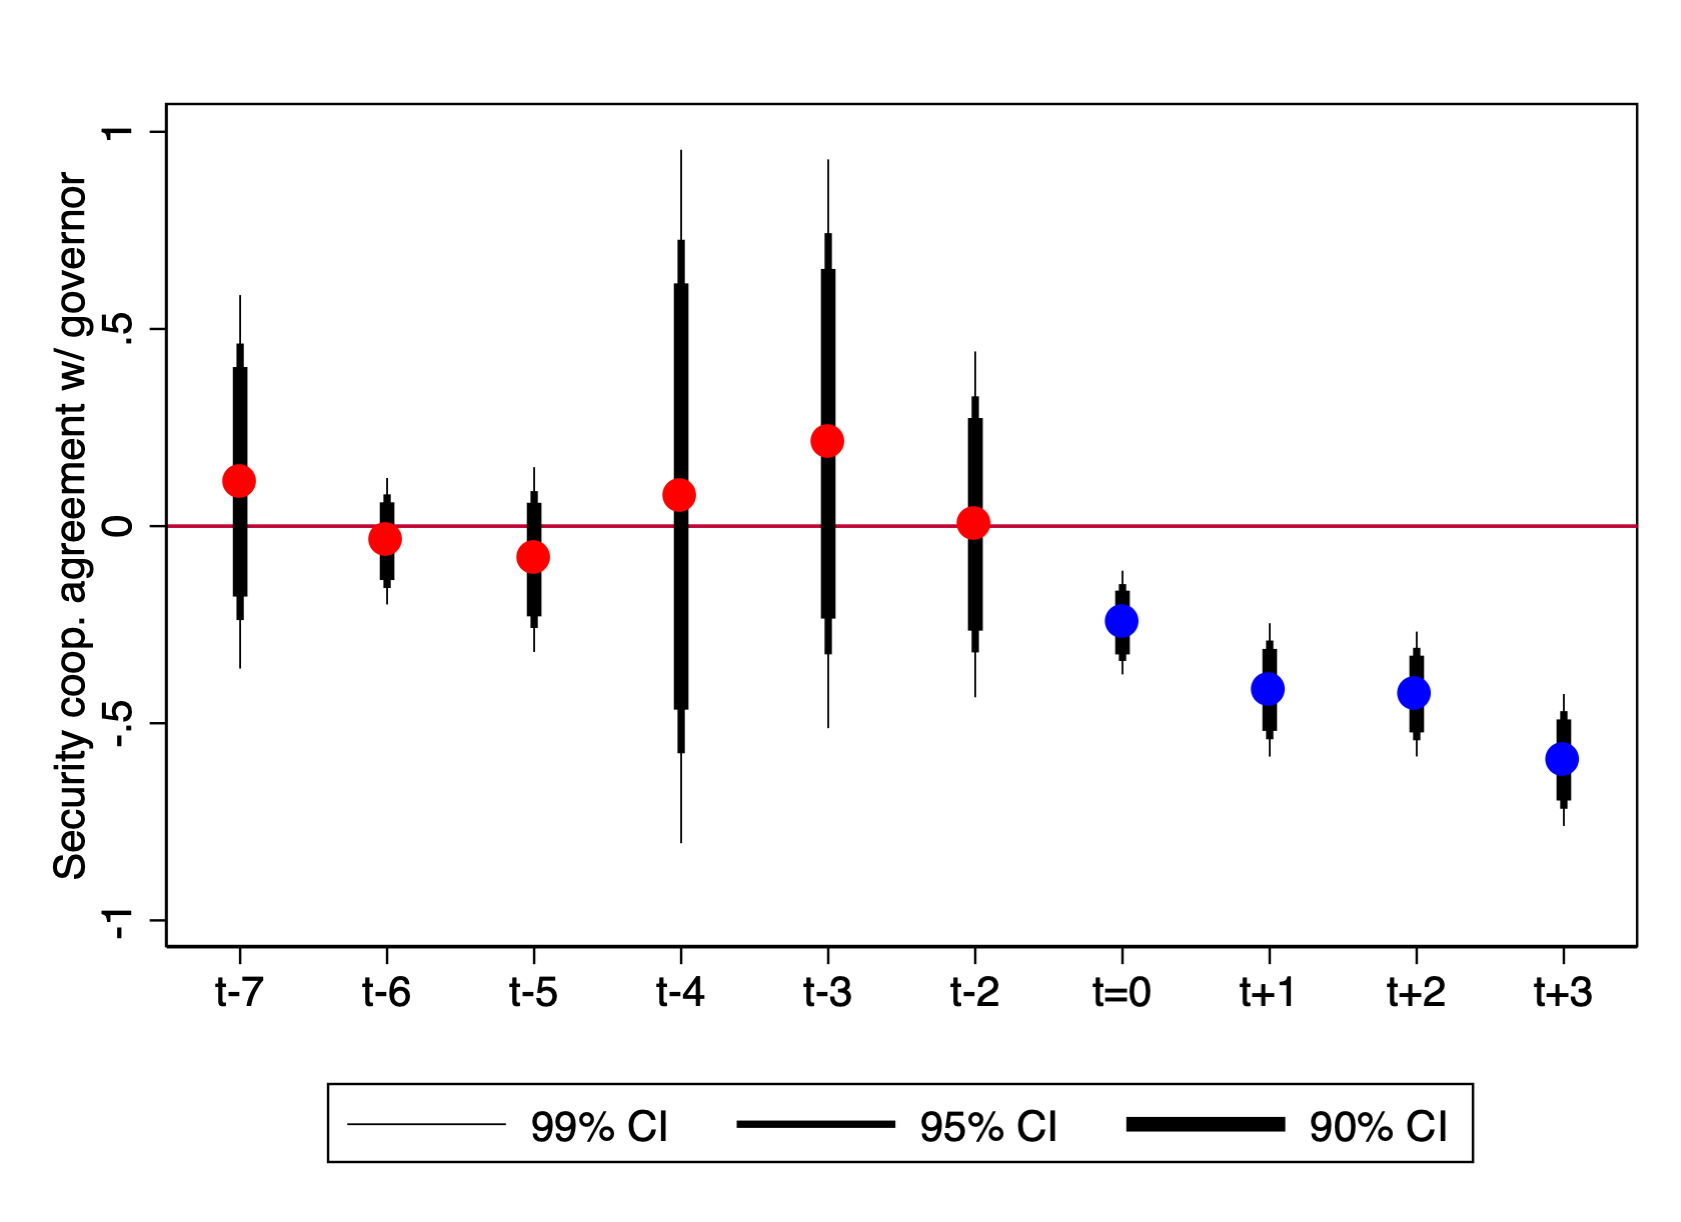
\includegraphics[width=0.75\textwidth]{Figures/catts_agreements.png}
       \captionsetup{justification=centering}
       
 \textbf{Note:} Figure \ref{fig:event_study_agreements} shows the IW estimators following \citet{abraham_sun_2020} for each lead and lag relative to the first year a municipality implemented reelection. Red points are pre-treatment, while blue ones post-treatment. 
     
\end{figure}   

 \begin{figure}[h]   
\centering
 \caption{Comparison: Security Cooperation Agreements with Governor vs. Other Actors, 2014-2018}
 \label{fig:services}
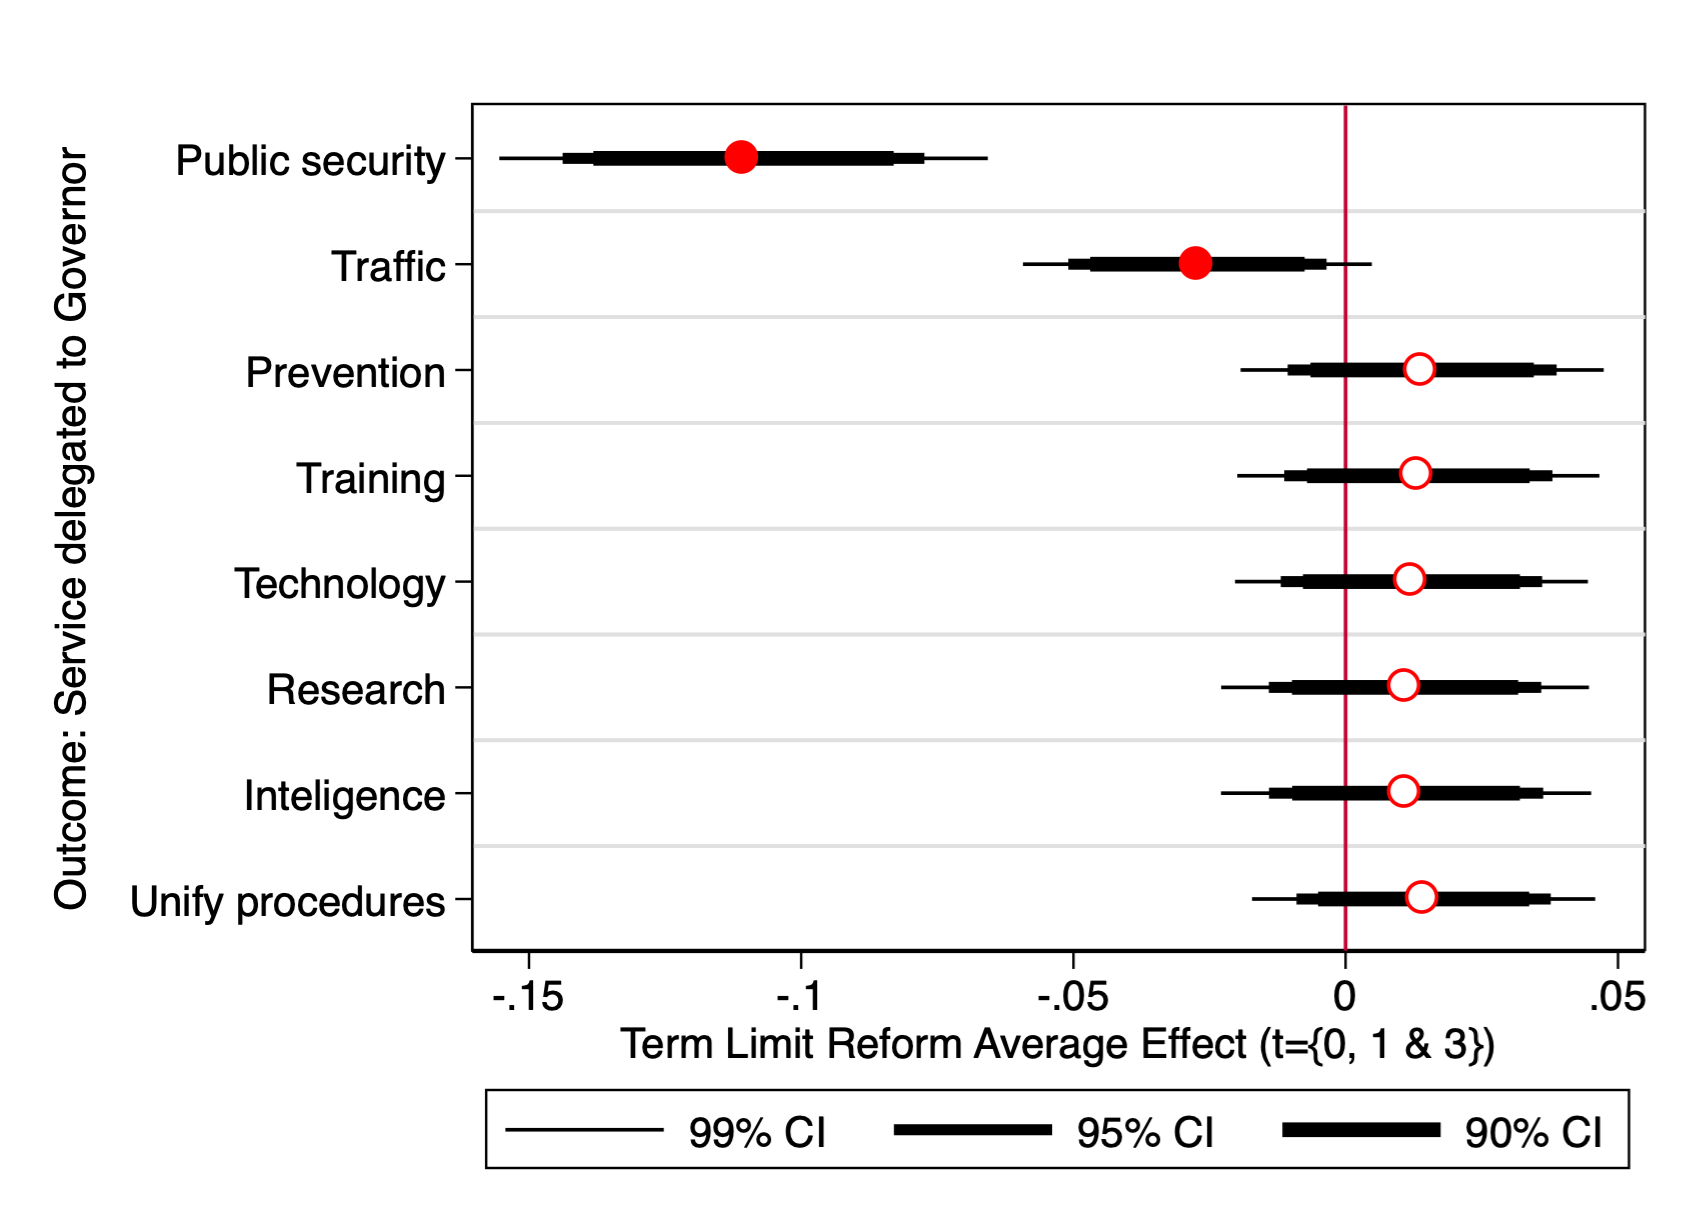
\includegraphics[width=0.65\textwidth]{Figures/services.png}
       \captionsetup{justification=centering}
       
 \textbf{Note:} Figure \ref{fig:services} shows the average treatment effect from t, t+1 and t+3 across multiple specifications. This average effect was estimated using the IW estimators following \citet{abraham_sun_2020} for each lead and lag relative to the first year a municipality implemented reelection. Red points show that parallel trends hold, while hollow ones imply pretrends. 
\end{figure}  

\subsection{Identification \label{sec:identification}}
 
Once we consider cohort weights, I find strong evidence of parallel trends as noted in Figure \ref{fig:event_study_agreements}.\footnote{Without cohort weights, the naive event-study design shows pretrends. However, these estimates are biased due to potential treatment effect heterogeneity across treatment cohorts.} Besides no pretrends, identification in this setting implies that the staggered roll-out of the Term Limit Reform is orthogonal to municipal-specific characteristics, conditional on municipal and year fixed effects. This implies {\emph as-if} random assignment to the treatment status visualized in Figure \ref{fig:treatment_status}. If say, strong governors delay or adjust the implementation of the reform according to their political agenda, then identification would fail. To address this problem equation \ref{eq:abraham} interacts the state covariates with cohort-specific fixed effects to adjust for any changes correlated to the evolution of governors strength, the term $X_{s(m)t} (1\{E_i=e\} \cdot R^k_{m,t})$. Pretreatment covariates include governor winning margin and an indicator of governor party alignment with the president, since pressure from former President Enrique Peña Nieto modified state legislators approval of the electoral reform, particularly for PRI states (for more detail see Appendix Section \ref{appendix:reform_backgorund}). Identification assumption implies now that conditional on municipal and year fixed effects, and cohort specific linear trends in state-level covariates, unobserved factors are not correlated with the electoral reform treatment assignment over time. I further validate this by following \citet{altonji_etal_2005} to check if unobserved variation is likely to explain the signing of centralized command agreements with the governor by mayors. I regress the treatment (whether the municipality held reelection) on all the available covariates used for Figure \ref{fig:event_study_agreements}. I then take the fitted value from the regression and use it to predict each outcome, this time including unit and year fixed effects. Appendix Table \ref{tab:unobservables} suggests that – under the assumption that observables are representative of unobservables – selection on unobservables is not driving the results. 

An additional identification assumption in event-study designs speaks to no anticipatory behavior from municipalities to the Term Limit Reform. If states or municipalities had private knowledge of the future treatment path this may change their behavior in anticipation to being treated and thus the potential outcome prior to treatment may not be that of baseline outcomes: estimated coefficients may reflect the anticipatory effects of the reform rather than differences in untreated potential outcomes between untreated and treated groups. %\citep{malani_rief_2015}.
%In this setting, knowledge from incumbents of the term limit removal could lead to a decrease in public security (and public good) provision since this will be the period a term limited politician could extract rents or pursue clientelistic practices without the electoral penalty of reelection. The violation of this identification assumption would lead to a (positive) bias of concern. 
I test this assumption by comparing if early and late adopters differed in their estimated effects. As seen in Appendix Figure \ref{fig:CDLZ_agreements}, this is not the case: there is wide variation in estimated coefficients across early (red) and late (blue) adopters of the reform.\footnote{For more detail on how I compare early to late adopters, please see Appendix \ref{appendix:CDLZ}.}  

In short, taking together parallel trends, evidence on no-anticipatory behavior from municipalities (and states) and cohort weighted estimates that account for treatment effect heterogeneity, I find a robust and unbiased negative effect of reelection incentives on the delegation of security policy from mayors to governors in Mexico.  The following sections further probe the results through different robustness and falsification tests.
         

\subsection{Robustness Tests and Secondary Research Designs \label{sec:robustness}}
 
  Figure \ref{fig:robustness_agreements} compares 6 models (see also Appendix Table \ref{tab:as_aggregate}). I find the naive two-way fixed effect model by municipality and year to reflect a negative non-significant effect of reelection incentives on delegation. However, pretrends are found and results need to be interpreted with caution as non-weighted estimates are biased \citep{abraham_sun_2020} as discussed in Section \ref{sec:design}. Adjusting standard errors using Wild bootstrap yields similar results for the naive two way fixed effect model. However, the main cohort weighted event study design with and without standard error adjustment using Wild bootstrap shows parallel trends and significant results. This result holds when changing the reference period from $t-1$ to $t=0$. Results also hold when performing the common practice of trimming relative time periods relative to treatment \citep{borusyak_2017, dobkin_etal_2018}, in this case by trimming all periods prior to $t-4$ to be balanced in relative periods. Moreover, across specifications the average effect from $t$ to $t+3$ remains relatively similar. 
        
  
\begin{figure}[h]   
\centering
 \caption{Effect of Term Limit Reform on Security Cooperation Agreements signed with the Governor, 2010-2018}
 \label{fig:robustness_agreements}
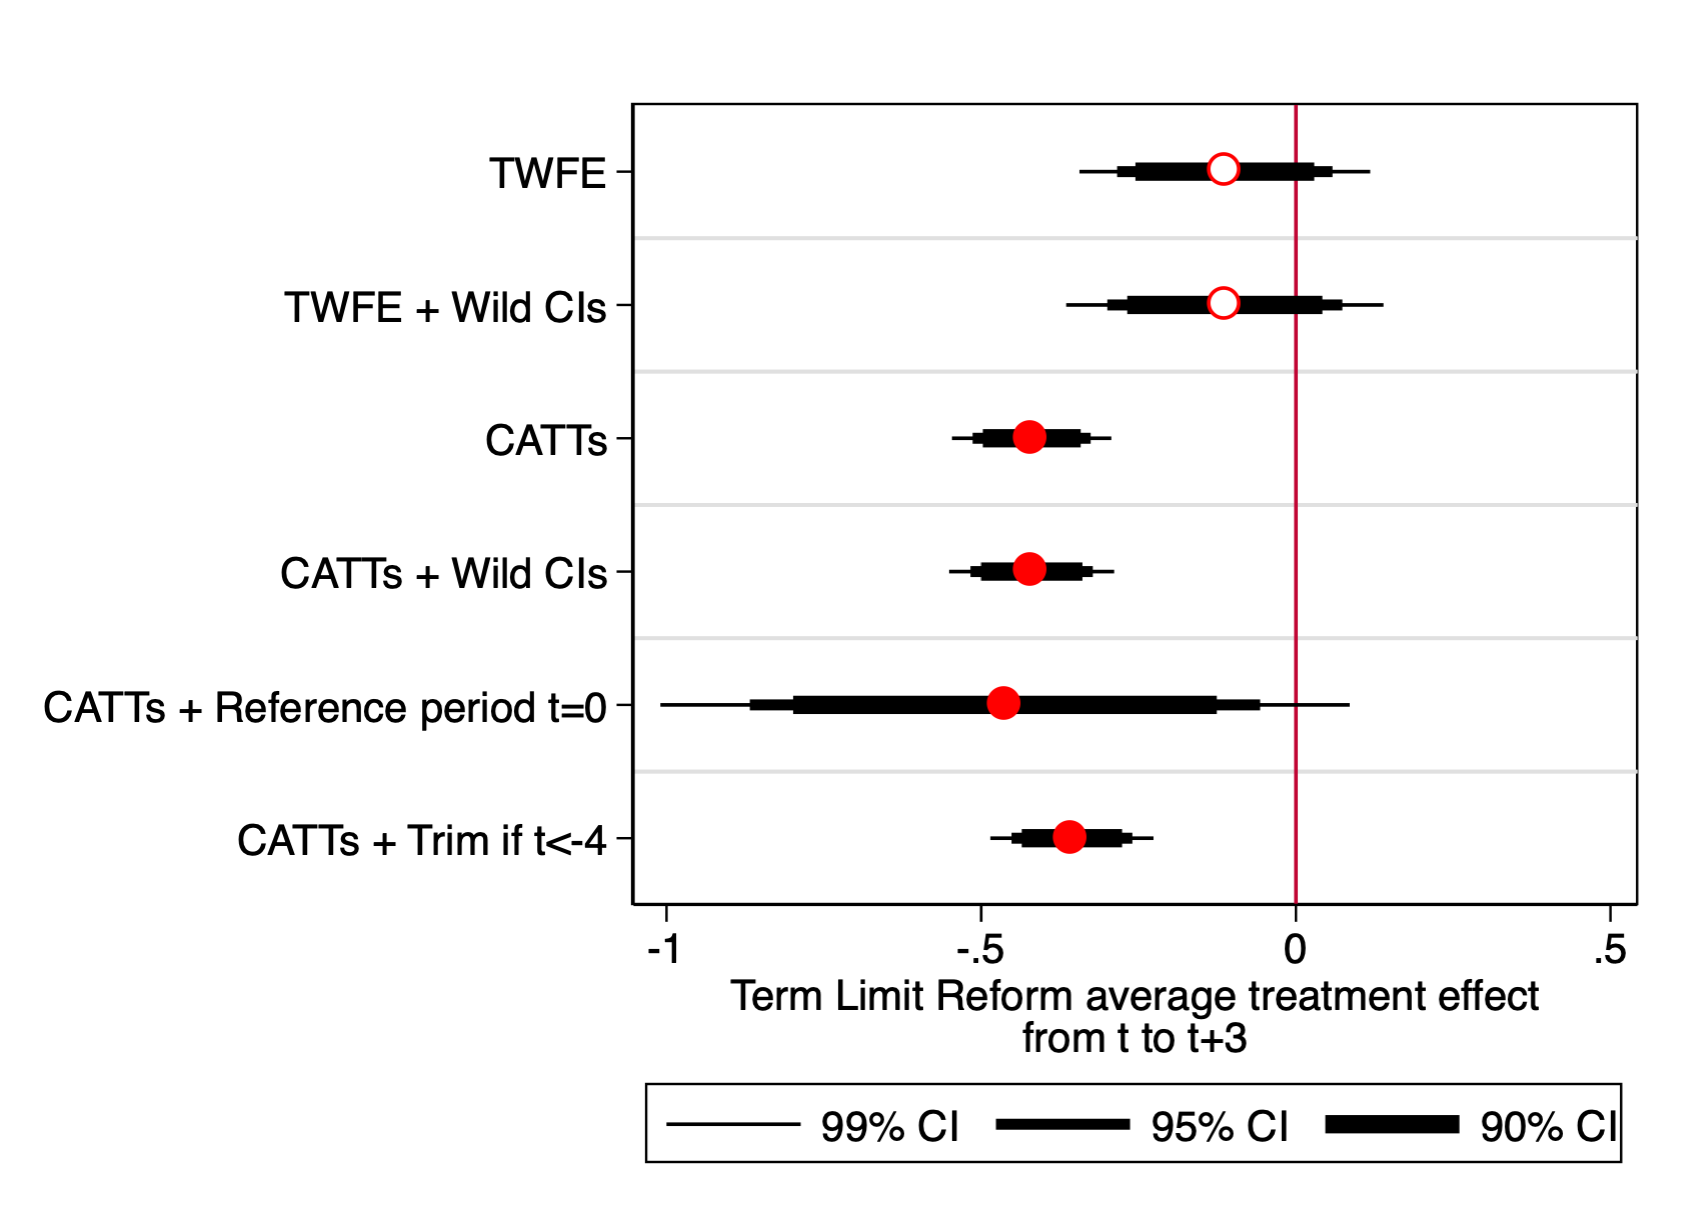
\includegraphics[width=0.75\textwidth]{Figures/average_effects.png}
       \captionsetup{justification=centering}
       
 \textbf{Note:} Figure \ref{fig:robustness_agreements} shows the average treatment effect from t to t+3 across multiple specifications. This average effect was estimated using the IW estimators following \citet{abraham_sun_2020} for each lead and lag relative to the first year a municipality implemented reelection. Red points show that parallel trends hold, while hollow ones imply pretrends. 
\end{figure}   

Further validation is provided by the use of secondary research designs including \citet{imai_etal_2020} non-parametric generalization of the difference-in-difference estimator that does not rely on linearity assumption and corrects for invalid negative weighting in standard two-way fixed effects models (see Appendix Figure \ref{fig:matching}), as well as \citet{chaisemarting_etal_2019} difference-in-difference with multiple time period correction (see Appendix Figure \ref{fig:chaisemarting_agreements}). In both cases we observe that reelection incentives led to a decrease in the signing of centralized command agreements, i.e. a decrease in delegation of security policy to the governor.

\section{Evidence on the Differentiation Mechanism\label{sec:heterogeneous}}

As discussed in Section \ref{sec:reelection_incentives}, we would expect incumbents with reelection incentives to send credit claim messages to portray competence or a strong type and difference themselves from challengers and the governor. They can do so by taking charge of security policy instead of delegating it to the governor. If this is true, we would expect this behavior to be more salient when  (i) citizens are concerned about violence, and (ii) when citizens are capable of rewarding or punishing mayors for security policy. 

\subsection{Heterogeneous Treatment Effects by Citizens' concerns}

In the context of American politics, for example, \citet{list_sturm_2006} find that governors seeking reelection adopt greener policies when their states hold large pro-environmental groups, while the opposite occurs in those with lower environmental support. In a similar tenor, we would expect that when a large proportion of citizens hold security concerns as the most worrisome topic then incumbents with reelection incentives will choose not to delegate security policy to the governor.   

This is what we find in Figure \ref{fig:preferences_all} Panel A that shows an interaction between the treatment of the Electoral Reform on narcotraffic as the topic that citizens´ worry the most. The baseline reform effect is statistically indistinguishable from zero. However, when a large proportion of citizens see narcotraffic as the topic they worry the most, mayors with reelection incentives decrease the delegation of security policy to governors relative to term-limit mayors. It is important to note that this finding is conditional on    pre-treatment violence levels, i.e. the differences in the concern of narcotraffic or delegation are not explained by differences in levels of violence but variation in idiosyncrasies between Mexican states.

 The same result is not find with insecurity or punishment to criminals as the topics that citizens worry the most. For insecurity we don't find parallel trends prior to treatment, and for punishment to criminals the result is not distinguishable from zero. More data on citizens security preferences would be needed to further validate the heterogeneous treatment effects found in Panel A. 
 
 However, to provide further validity Figure \ref{fig:preferences_all} Panels D to L run a placebo test:  they include other topics that citizens worry the most but are not related with public security provision. Since these topics are not related to security policy we should expect a null result. This is what we find and, in some cases, even positive interaction effects. These positive cases belong to topics that are of the national order in which cooperation with upper level governments is needed such as natural disasters and water scarcity. Interestingly, in these two cases the state and federal security forces, specially the military, have a very important role to solve the problem. 
 
\begin{figure}[h]   
\centering
 \caption{Electoral Reform Interaction Effects by Topic that Worries Most to Citizens}
 \label{fig:preferences_all}
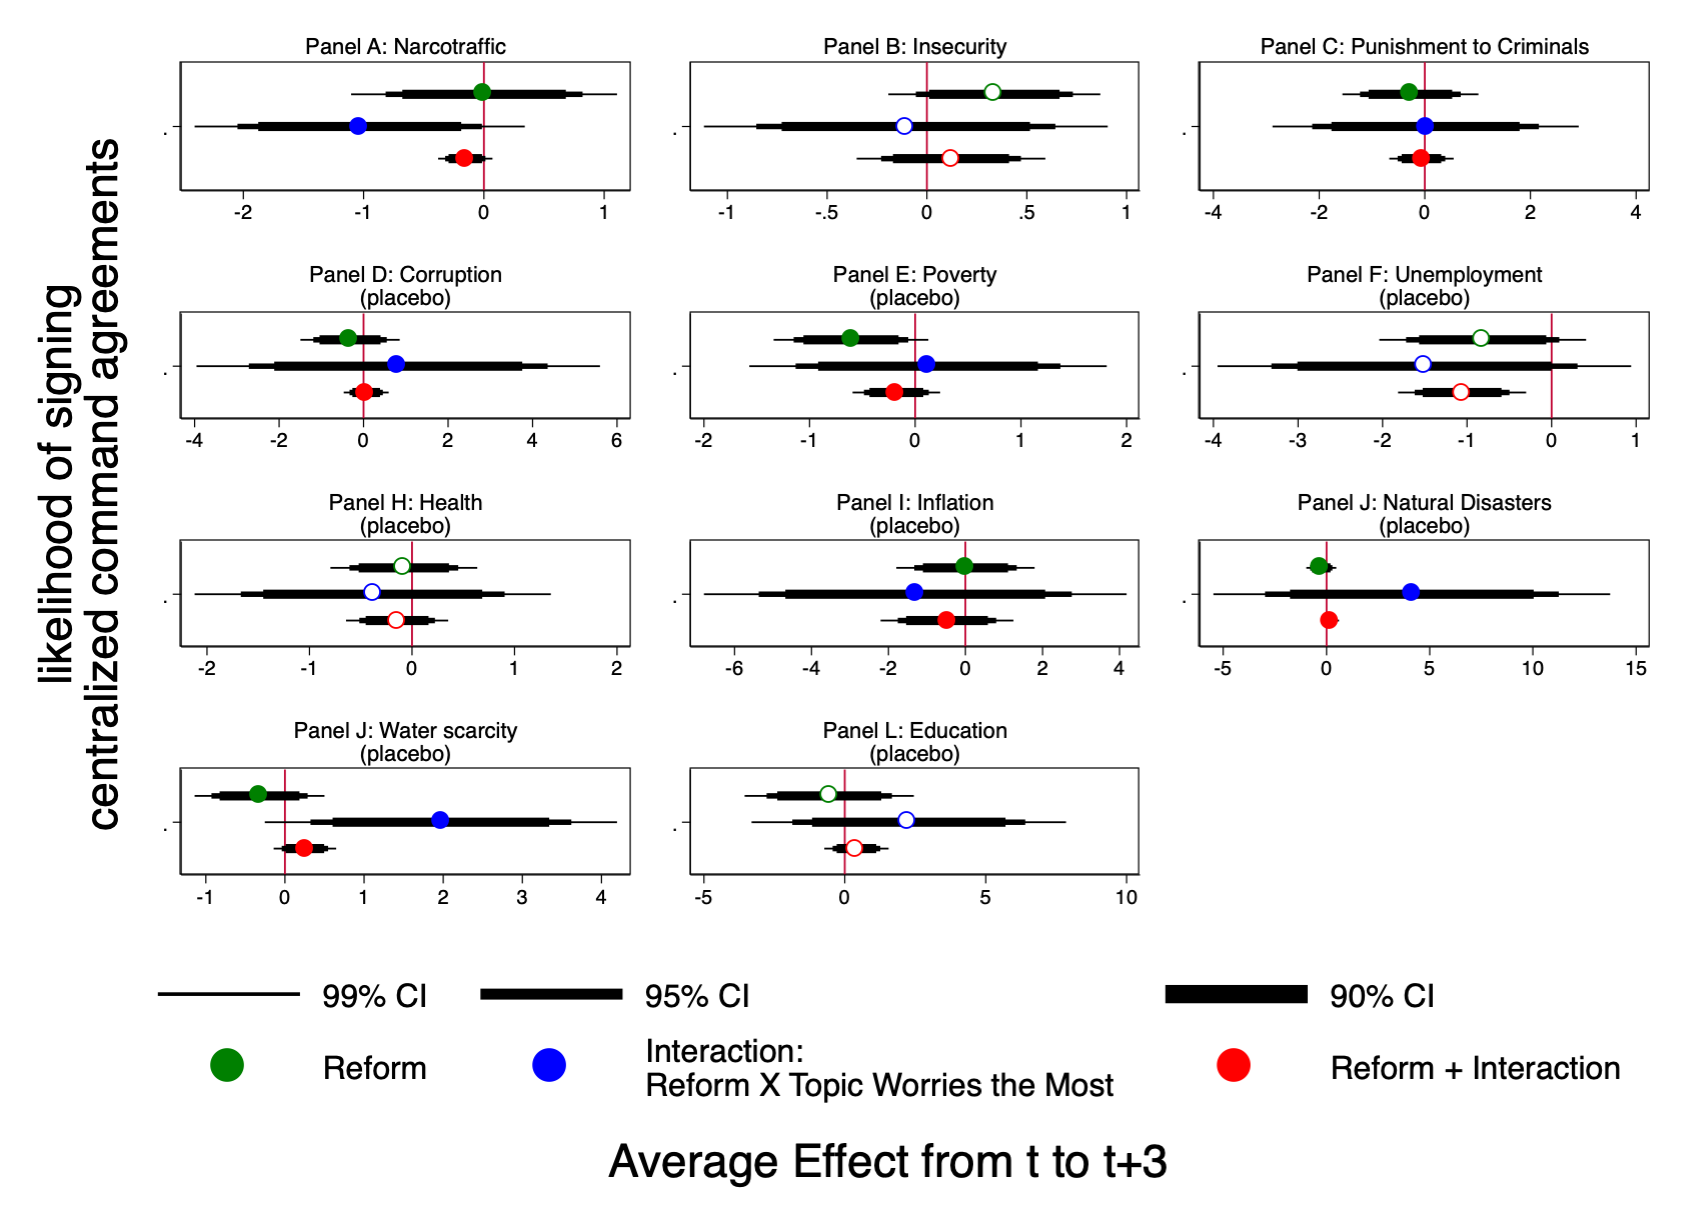
\includegraphics[width=1\textwidth]{Figures/preferences.png}
       \captionsetup{justification=centering}
        
 \textbf{Note:} Figure \ref{fig:preferences_all} shows the estimates of interacting the 2014 Term Limit Reform on the proportion of citizens that state that the topic stated worries them the most. This beliefs are pre-treatment. Point estimates show the average treatment effect from t to t+3. This average effect was estimated using the IW estimators following \citet{abraham_sun_2020} for each lead and lag relative to the first year a municipality implemented reelection. Filled points show that parallel trends hold, while hollow ones imply pretrends.  
\end{figure}    


\subsection{Heterogeneous Treatment Effects by Citizens Capacity to Determine Mayors as Responsible for Security Policy}
  
For incumbents with reelection incentives to care to impress voters, citizens need to be able to blame and reward incumbents for local security policy. In the case of Mexico, \citet{ley_2017} shows that citizens hold the capacity to blame (and reward) mayors for security policy if their party is aligned with that of the governor. Therefore, if there is alignment with the governor, we should expect mayors to decrease the delegation of security policy to differentiate themselves. In contrast, with alignment with other political actors like the president, citizens cannot clearly identify the responsible decreasing the incentive mayors have to differentiate themselves from other political actors by taking charge of security policy. In this case null results should be expected. Consider this a placebo test.
  
Figure \ref{fig:alignment} shows the interaction effect of party alignment on the Term Limit Reform. As expected in the interaction of Panel A, when there is alignment with the governor mayors up for reelection decrease the delegation of security policy to the governor, a result significant to the 5\% level. However, when not aligned as showed by the reform baseline result the coefficient is not different from zero. 

In contrast, in Panel B on the alignment with the president we find null results (and slightly positive) as expected, since citizens cannot assign responsibility to mayors for public security provision. 

\begin{figure}[h]   
\centering
 \caption{Reform interaction with Party Alignment}
 \label{fig:alignment}
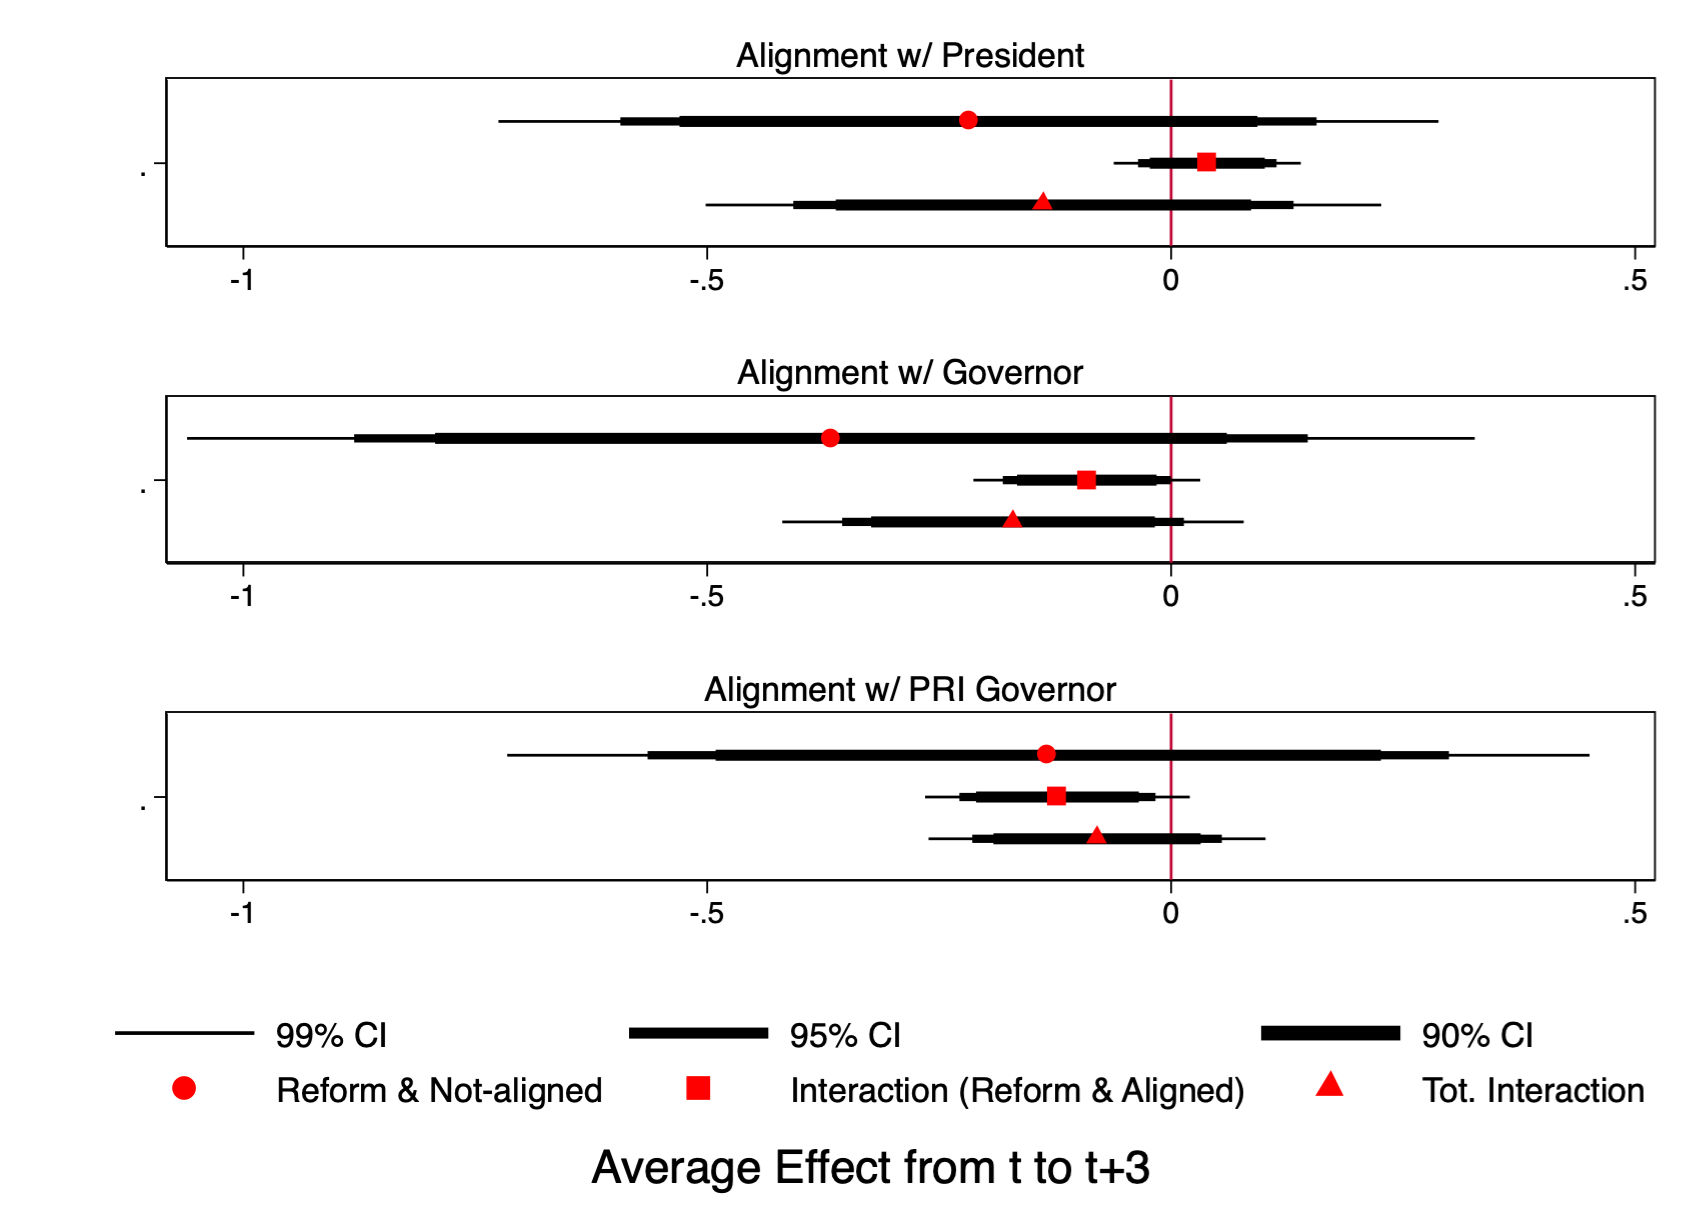
\includegraphics[width=0.9\textwidth]{Figures/interaction_alignment_full.png}
       \captionsetup{justification=centering}
       
 \textbf{Note:} Figure \ref{fig:alignment} shows the average treatment effect from t to t+3 across multiple specifications. This average effect was estimated using the IW estimators following \citet{abraham_sun_2020} for each lead and lag relative to the first year a municipality implemented reelection. Red points show that parallel trends hold, while hollow ones imply pretrends. To check parallel trends see Appendix Figure \ref{tab:interaction_alignment}.  
\end{figure}  
	
\subsection{Further validity on the differentiation mechanism: A Placebo Test on Security Agreements with Other Political Actors}


Now, I run a placebo test by seeing the effect of the reform on security cooperation agreements signed with the president, governors from other states and other municipalities. As described in the Data Section \ref{sec:data}, this security cooperation agreements serve as placebos as mayors do not hold an interest to differentiate themselves from these actors,  since the president's federal security forces do not deal with local public security, and governors and mayors from other states and municipalities are no electoral challengers. As expected, the falsification test in Figure \ref{fig:comparison_fed_estatal} shows a positive and non-significant effect for signing security cooperation agreements with other actors besides the governor. Meanwhile, similar to centralized command agreements, for security cooperation agreements with the governor in which the mayor continues to exercise responsibility in public security policy (i.e. these agreements do not imply delegation) we see a negative and significant effect. Mayors up for reelection choose to decrease not only the delegation of public security but also the reliance of any other type of cooperation agreements with the governor to whom they wish to differentiate themselves, and to differentiate from challengers as well.    
  
 \begin{figure}[h]   
\centering
 \caption{Comparison: Security Cooperation Agreements with Governor vs. Other Actors, 2014-2018 \\ -outcome: signing security cooperation agreement-}
 \label{fig:comparison_fed_estatal}
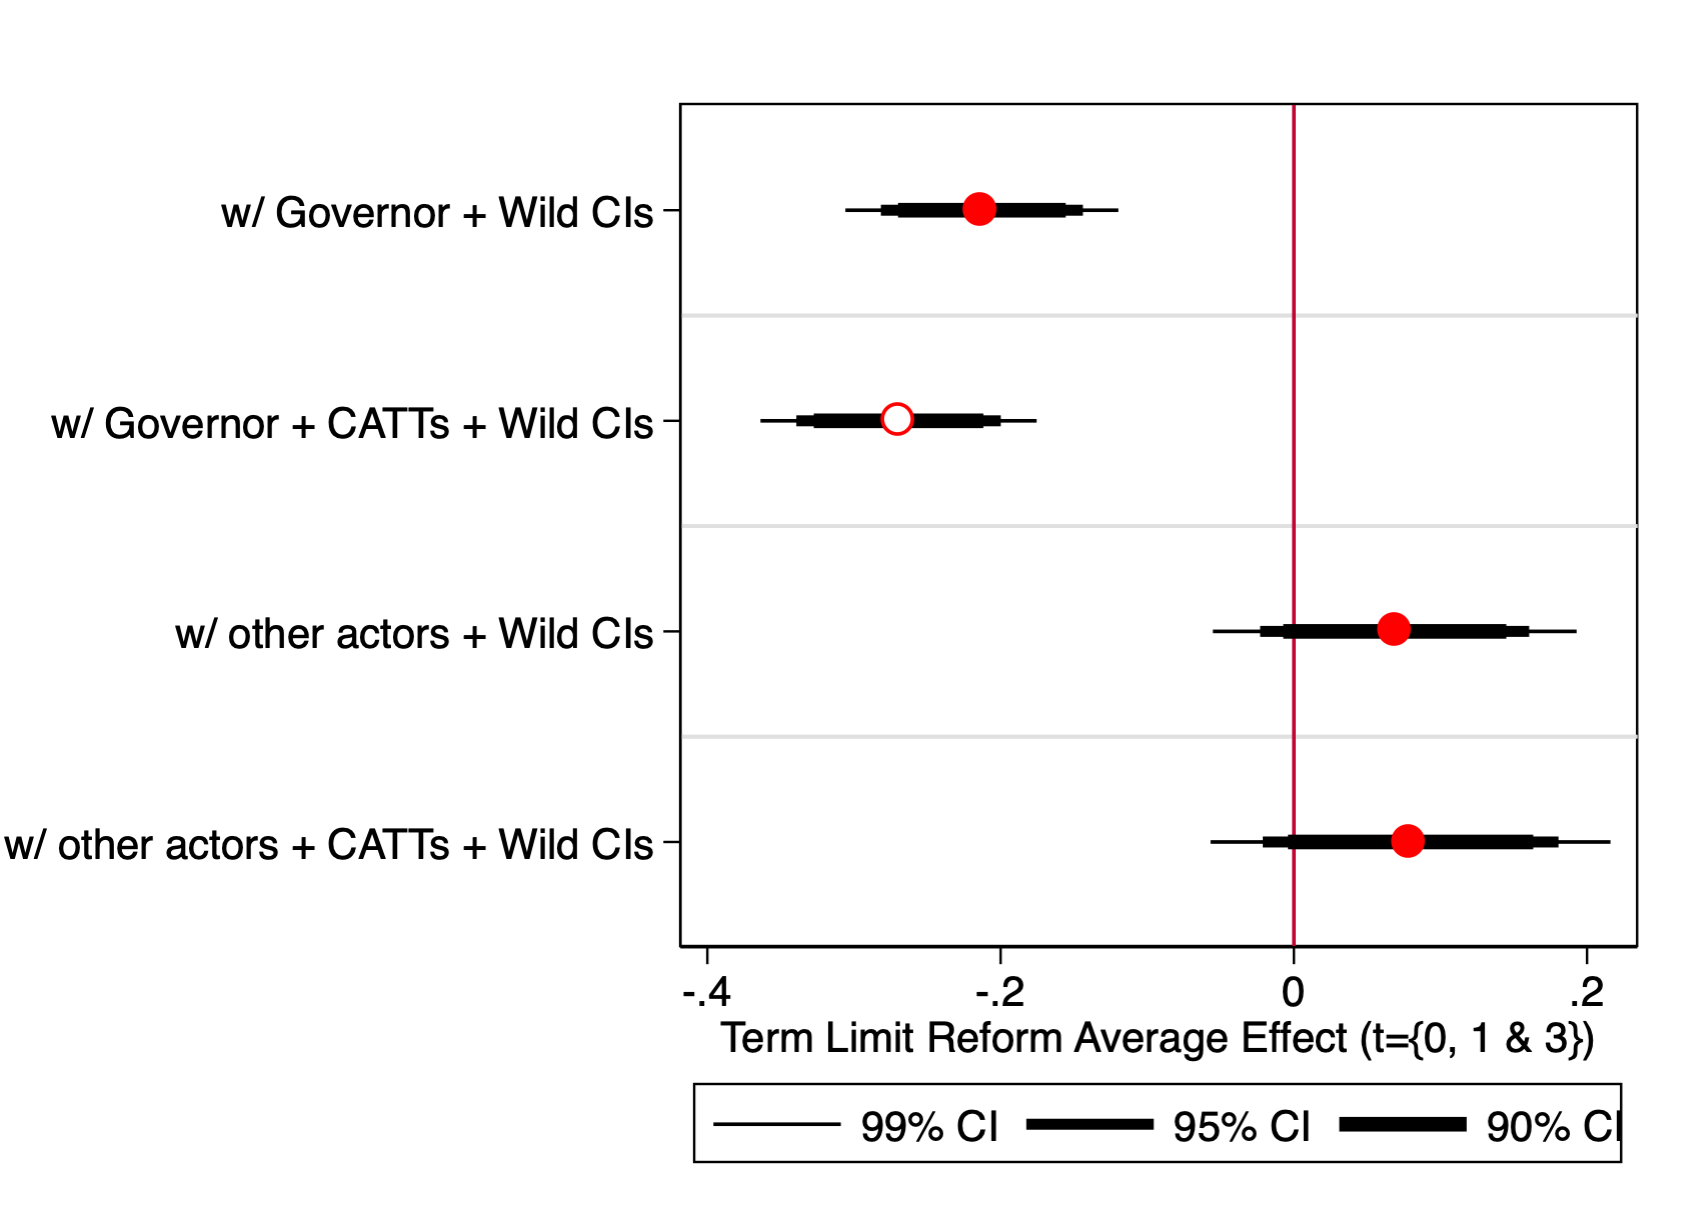
\includegraphics[width=0.75\textwidth]{Figures/average_effects_comparisonfedest.png}
       \captionsetup{justification=centering}
       
 \textbf{Note:} Figure \ref{fig:comparison_fed_estatal} shows the average treatment effect from t to t+3 across multiple specifications. This average effect was estimated using the IW estimators following \citet{abraham_sun_2020} for each lead and lag relative to the first year a municipality implemented reelection. Red points show that parallel trends hold, while hollow ones imply pretrends. 
\end{figure}   

\subsection{Credit Claiming or Responsiveness?}

As discussed in Section \ref{sec:reelection_incentives}, it is important to differentiate between credit claiming and responsiveness, i.e. between an exercise to send a signal to voters or actually addressing voters concerns. The difference is not minimal, as the latter implies the strengthening of accountability while the former does not. A way to empirically disentangle these two mechanisms is to assess the level of effort placed by mayors to tackle organized crime. 

Figure \ref{fig:effort} shows that while the effort placed by the local police in municipalities with mayors seeking reelection remains similar to that of term-limited incumbents as measured by the number of detentions per capita made by the municipal police, we observe a decrease in anti-narcotic activities by federal and state-level forces. Since we condition for pre-treatment levels of violence, we could consider these measures as proxies for effort. Therefore, there is no difference in the level of effort placed by mayors up for reelection to those that are term-limited which could be an evidence of credit claiming rather than responsiveness. Moreover, results show that the effort of federal forces does decrease leaving mayors to their luck to fight crime.

\begin{figure}[h]  
\centering
\caption{Effect of Term Limit Reform on Effort of Local and Federal Security Forces} 
\label{fig:effort}

   
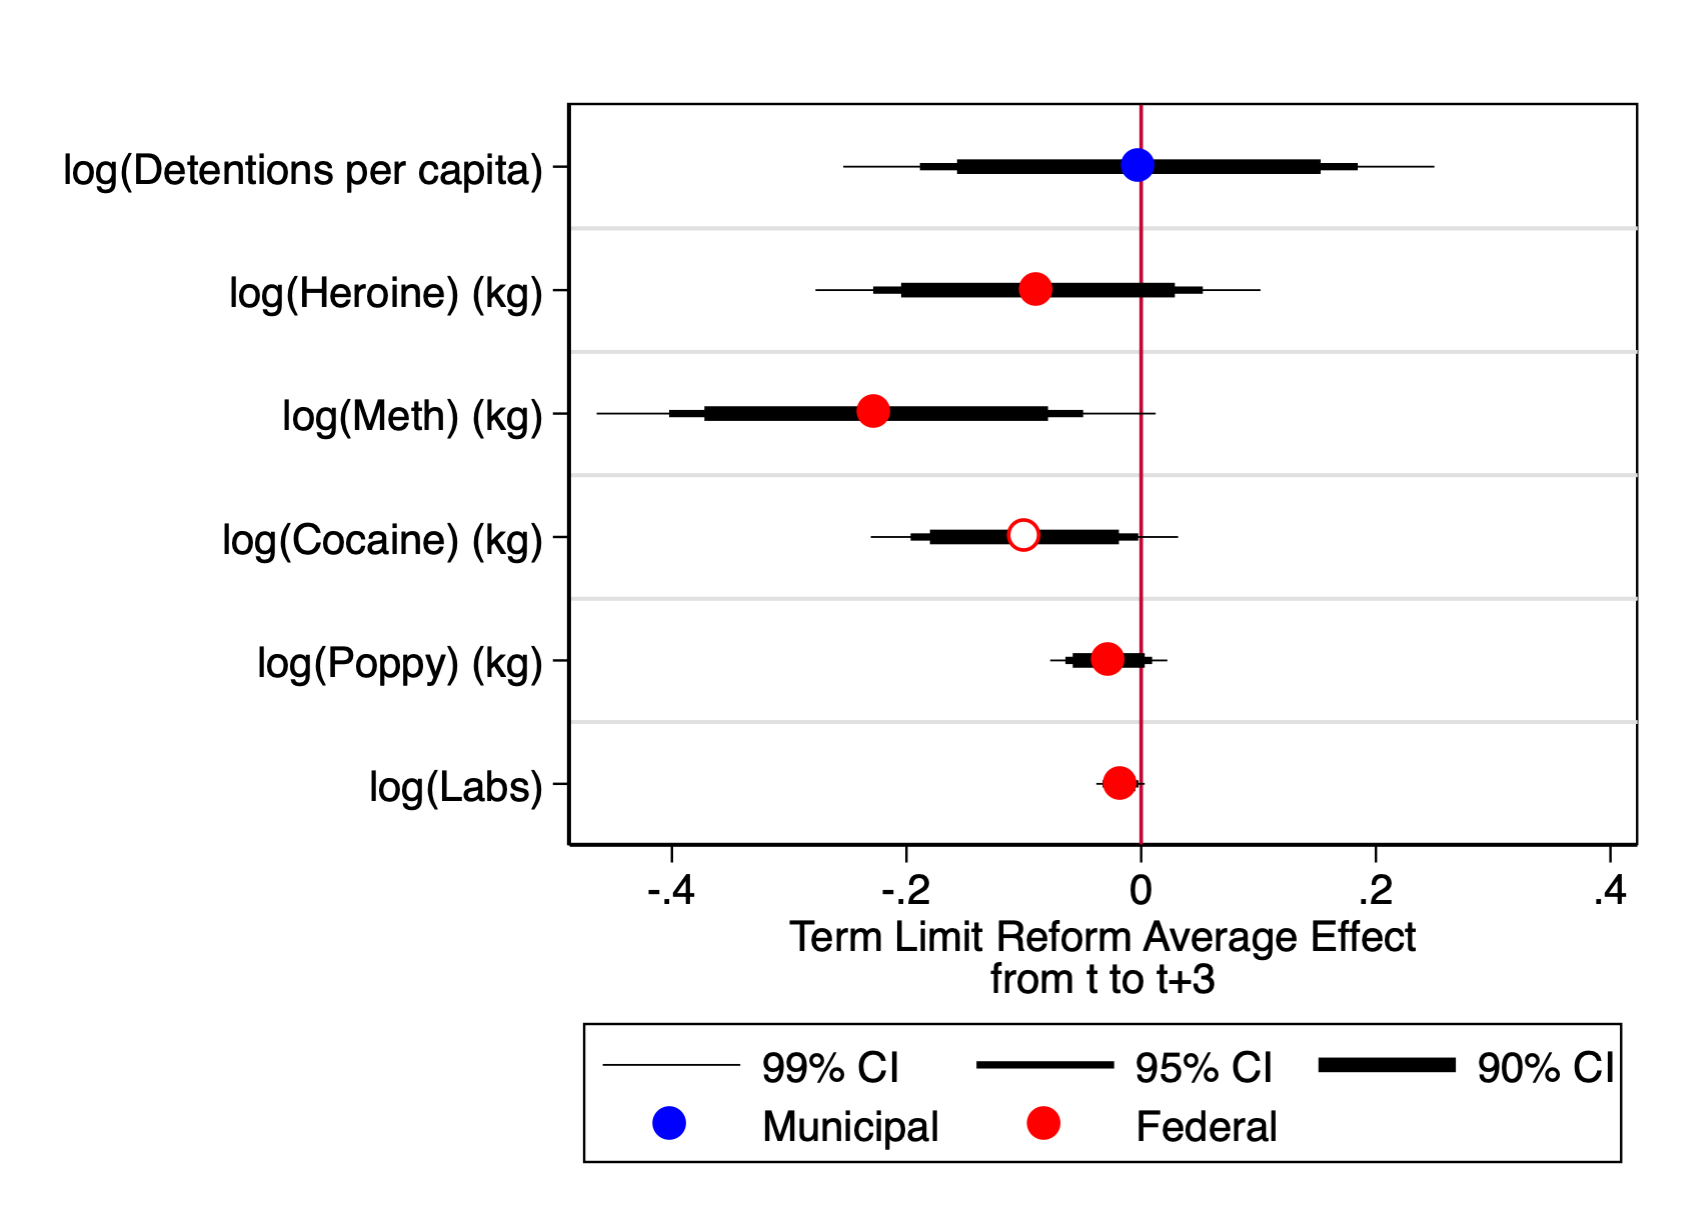
\includegraphics[width=0.75\textwidth]{Figures/effort.png}
  
 \textbf{Note:} Figure \ref{fig:effort} shows the average treatment effect from t to t+3 across multiple specifications. This average effect was estimated using the IW estimators following \citet{abraham_sun_2020} for each lead and lag relative to the first year a municipality implemented reelection. Filled points show that parallel trends hold, while hollow ones imply pretrends.        
\end{figure} 

If there are concerns that anti-narcotic measures or local police force detentions proxy for violence and not effort, we can rely on another measure of effort placed by mayors in office: expenses in public security. Figure \ref{fig:expenses} shows mayors up for reelection decreased their expenses in public security, while no changes in the wages of bureaucrats was noticed relative to term limit mayors. These wages include the wages to local police forces. %A similar decrease in the expenses on security are noticed in social development and infrastructure, with the latter including expenses related to building new training and monitoring centers, as well as other police centers. 
While there might be a concern of a decrease in municipal revenues that could explain these results, \citet{ch_2021} shows that mayors up for reelection in Mexico not only increased their municipal revenues through an increase of local tax revenues, but also saw an increase in the total amount of transfers received from the federation and the state. In conclusion, mayors up for  reelection seem not to increase the deterrence of criminal organizations as measured by effort placed to do so. This makes mayors interested in sending signals to voters on willingness to take charge of security policy rather than being responsive to citizens security demands. 
  
 \begin{figure}[H]   
\centering
 \caption{Effect of Term Limit Reform on Municipal Expenses}
 \label{fig:expenses}
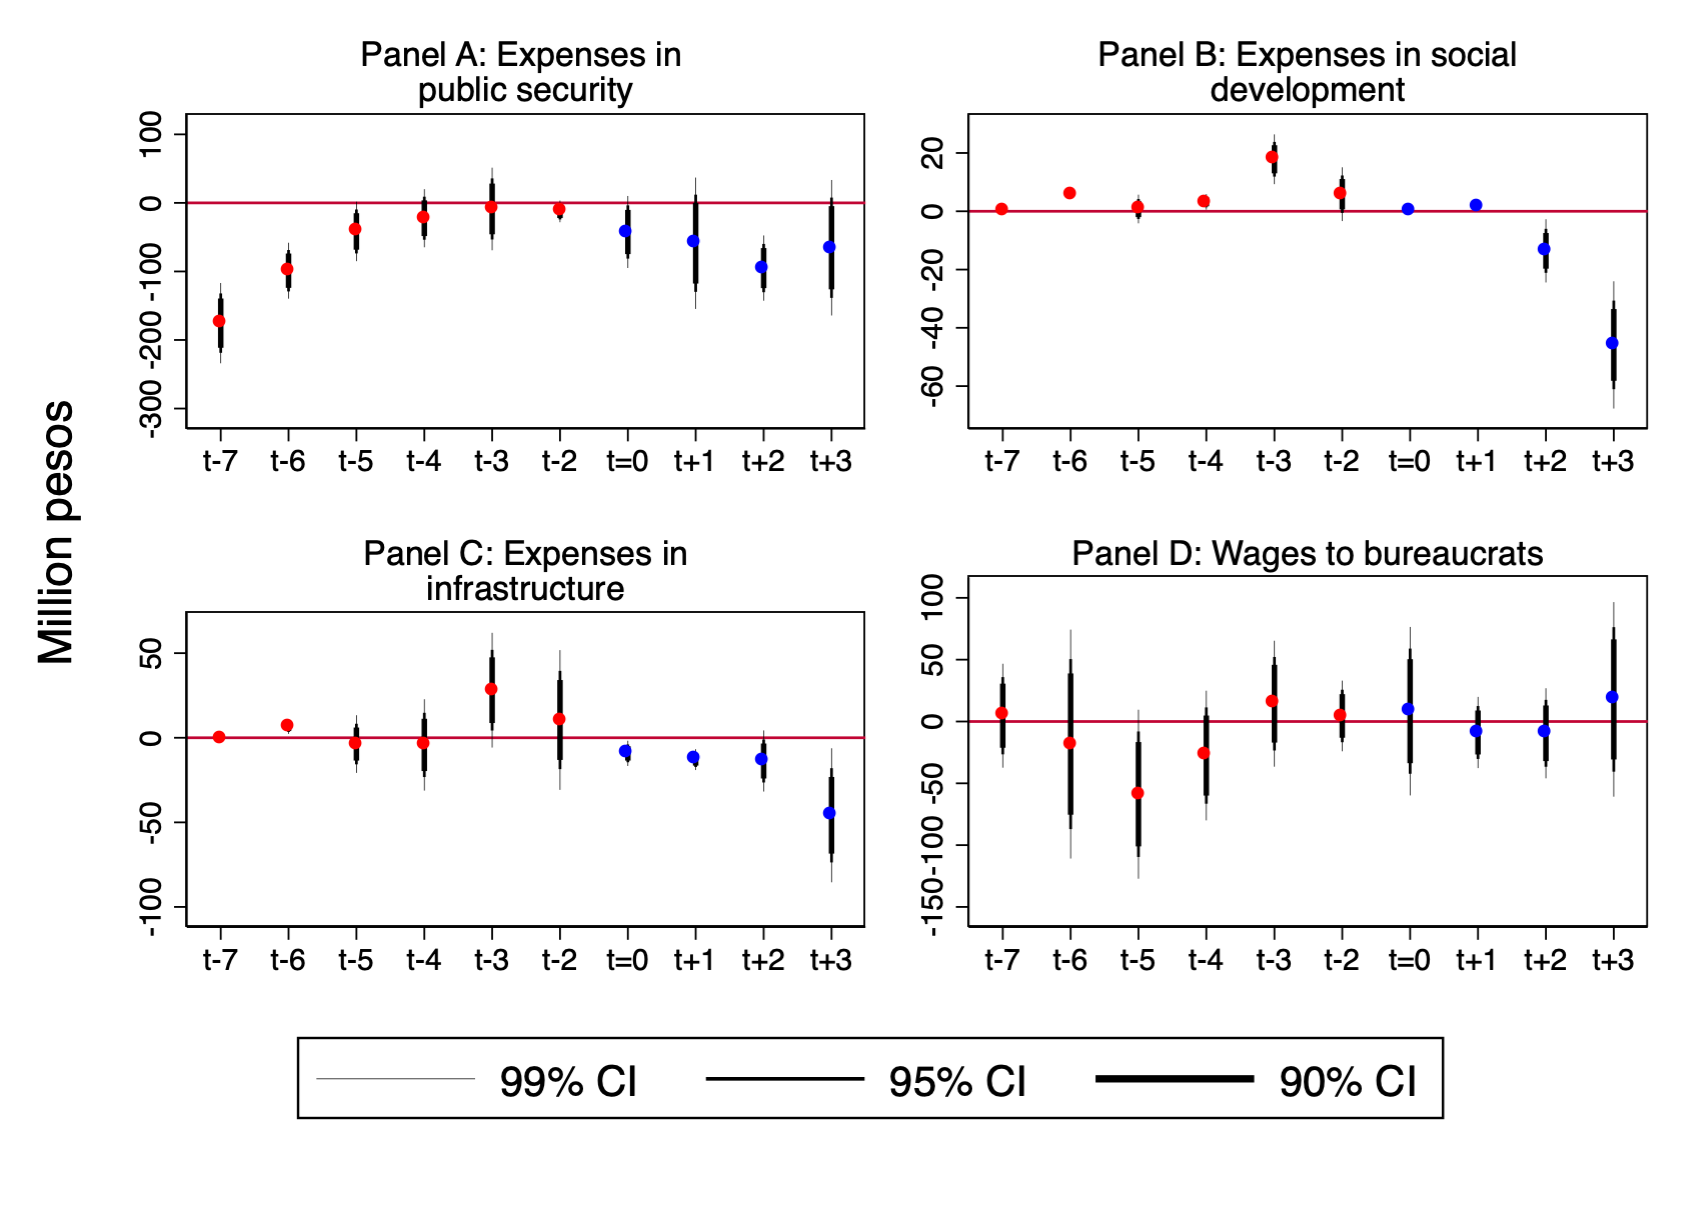
\includegraphics[width=0.9\textwidth]{Figures/expenses_allyears.png}
       \captionsetup{justification=centering}
         
 \textbf{Note:} Figure \ref{fig:expenses} shows the IW estimators following \citet{abraham_sun_2020} for each lead and lag relative to the first year a municipality implemented reelection. Red points are pre-treatment, while blue ones post-treatment. 
                     
\end{figure}   


\section{Consequences of Mayors Taking Charge of Security Policy: Violence \label{sec:unintended}}


What are the results of mayors up for reelection not delegating security policy to more capable agents like the governor? Until now, I have assumed that the public security provision is a more efficient endeavor under the hands of governors who can pool a greater amount of resources, information, skills and expertise than mayors. Moreover, given the high presence of spillovers delegation seems to be the most efficient way to achieve the monopoly of violence \citep{oates_1972}. Figure \ref{fig:as_violence} reports the reduce form IW estimators for each lead and lag relative to the first year a municipality implemented reelection. Results show a negative effect of reelection incentives on violence. On average, from $t$ to $t+3$, homicides per capita increased in 10.4\% using a logarithmic transformation and 6.6\% using the inverse hyperbolic transformation, significant to the 5 and 10\% respectively. As Appendix Figure \ref{fig:robustness_violence} shows, results are robust across multiple specifications including changing the reference period of the reform and adjusting for the small number of clusters (states) using Wild bootstrap. Further validation is provided by the use of \citet{imai_etal_2020} non-parametric generalization of the difference-in-difference estimator that corrects for invalid negative weighting in standard two-way fixed effects models through propensity score matching (see Appendix Figure \ref{fig:matching_violence}). 


\begin{figure}[h] 
\centering
 \caption{Effect of Term Limit Reform on Violence}
 \label{fig:as_violence}
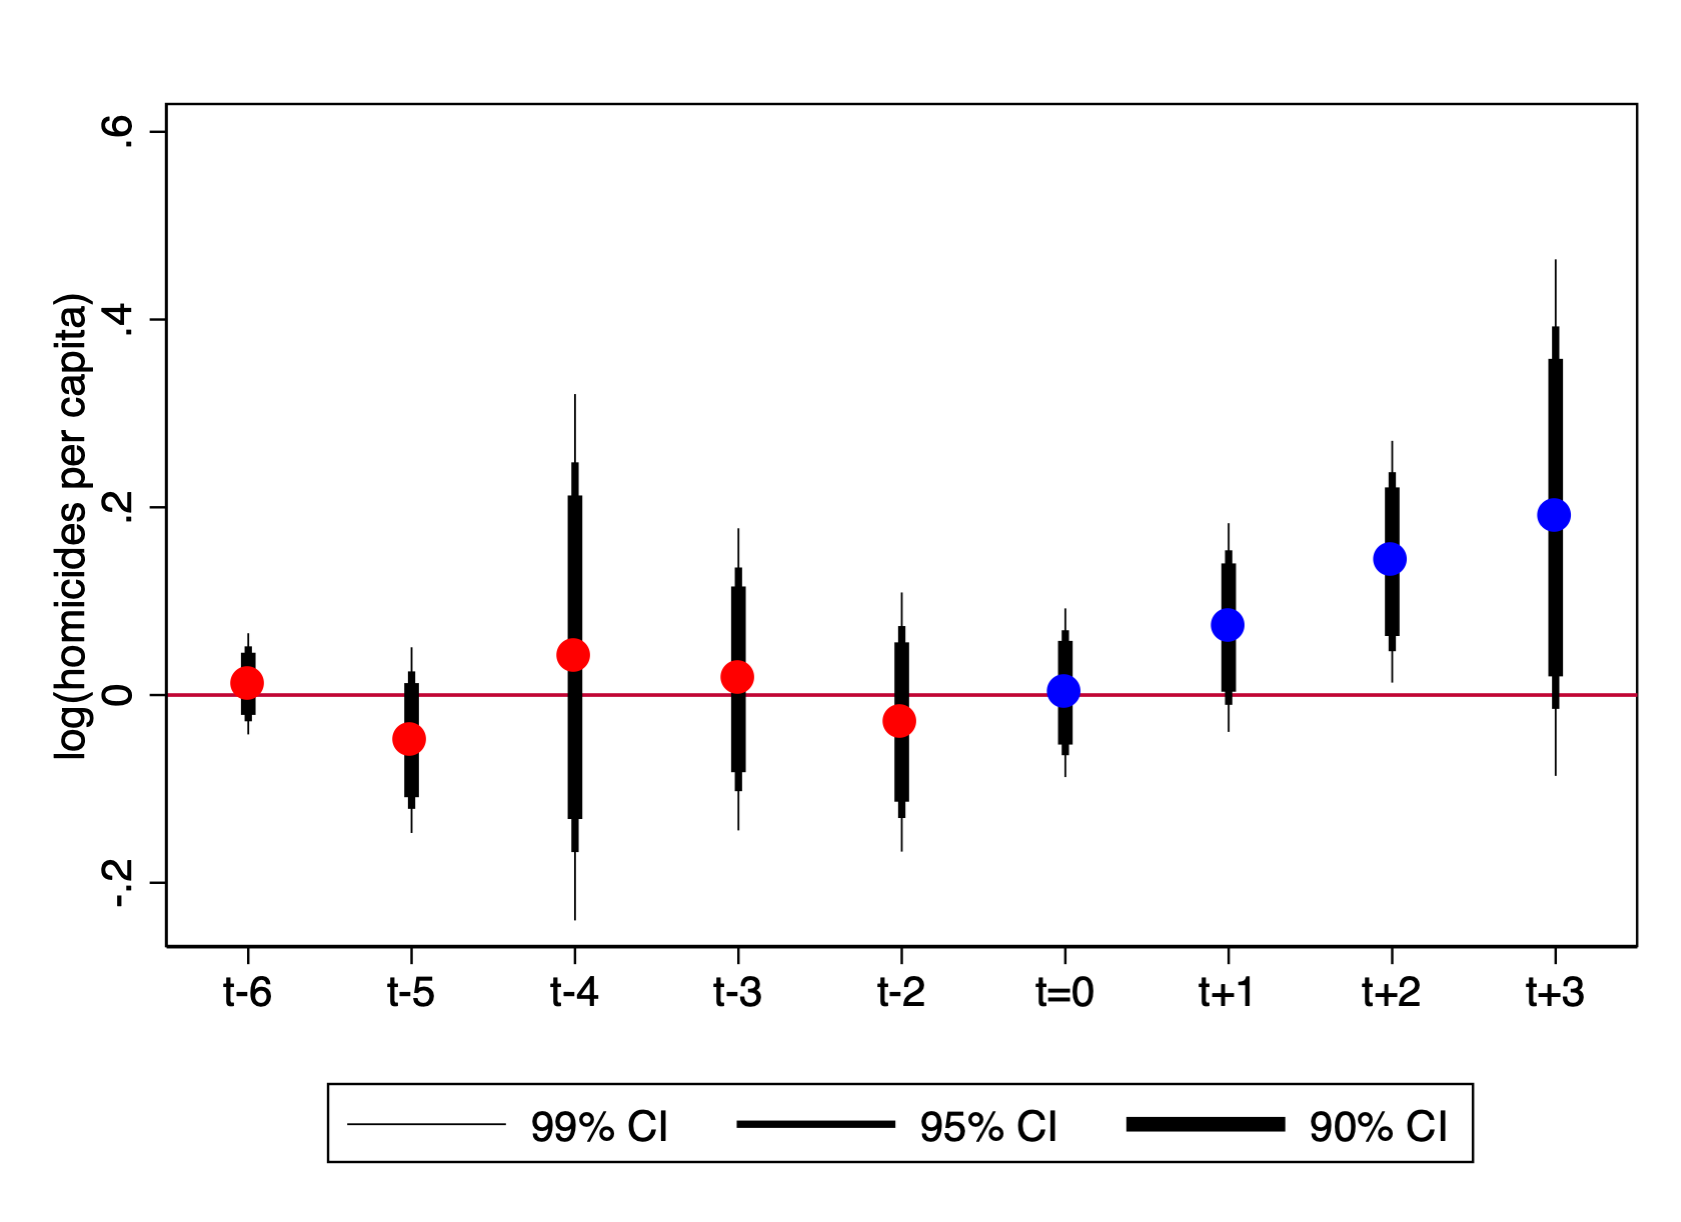
\includegraphics[width=0.9\textwidth]{Figures/catts_homicides.png}
       \captionsetup{justification=centering}
       
 \textbf{Note:} Figure \ref{fig:as_violence} shows the IW estimators following \citet{abraham_sun_2020} for each lead and lag relative to the first year a municipality implemented reelection. Red points are pre-treatment, while blue ones post-treatment. 
    
\end{figure}    

Why do voters do not punish mayors for the increase in violence? Overall, constituents lack the capacity to assess if violence increase in their locality. This problem is even more worrisome when mayors control local news outlets as is the case in the majority of municipalities in Mexico. Moreover, mayors control the spin of local news as many use a media strategy to showcase their competence to fight crime but say it will take a while till peace is achieved. This strategy was widely used by the Felipe Calderon administration in Mexico during his first years in office when violence increased dramatically across the country. Politicians also tend to blame corruption for the increase in violence, arguing that violence increased since corrupt politicians are no longer capable of protecting criminal groups. \citet{ch_2021} further shows that incumbents up for reelection experience a positive incumbency return mainly due to an increase in the resources of the municipality. In other words, increasing resources rather than decreasing welfare due to violence makes citizens sustain mayors in office, while they expect a higher budget or transfer in the future will accrue directly to them. 

\section{Conclusion \label{sec:conclusion}}

This paper studies a classic problem faced by governments with a supra-entity capable of providing and delivering public goods: to delegate or not to delegate. Specifically, it delves into an understudied phenomenon of delegation, the role of reelection incentives. I find that reelection encourages mayors to focus on policies with the highest “electoral yield”—namely, not to delegate public security to the governor. Why? By directly delivering public security mayors can differentiate themselves from others sending a signal to voters on their competence and strong type capable of battling organized crime. This behavior is predominant when citizens are concerned about narcotraffic and when citizens are capable of blaming or rewarding local politicians, i.e. when incumbents seeking reelection are aligned with the party of the governor. This behavior, is a pure credit claiming behavior as in reality mayors do not increase their level of effort to tackle crime, and thus are not responsive to citizens security demands. In other words, in terms of security policy reelection incentives did not strengthen accountability to voters. Since delegation of local security policy to the governor is the most efficient choice in this setting, reelection incentives lead to an inefficient outcome: an increase in violence. These results suggests that reelection incentives may lead incumbents to differentiate themselves by tacking charge of policy at the expense of inefficiency. This makes delegation not only a policy but an electoral decision. 

It is important to acknowledge certain caveats of this paper and avenues for future research. A reason why reelection may decrease delegation to upper-level governments is state capture. %Public good provision entails, sometimes, the interaction with a third player. %For example, incumbents interrelate with firms who compete for procurement bids. In the process, however, incumbents may be captured, changing the market structure and decreasing welfare. This is even more prevalent with longer tenures \citep{coviello_etal_2017}. As noted by  \citet{canen_etal_2020} influence groups are strategic and react to the uncertainty of the political environment by capturing the local apparatus. 
Incumbents may be captured by non-state armed groups who modify local institutions in favor of their self interest \citep{ch_etal_2018}, including a reduction in state-led violence agains them which could be achieved by not delegating security policy to more capable agents like the governor.  Moreover, a more nefarious read of the results of this paper is that incumbents up for reelection  do not delegate policy to the governor to have the capacity to flexibly negotiate terms with criminal groups. This mechanism does not invalidate the differentiation mechanism described in the paper but adds a future mechanism to explore. 

Lastly, is its important to consider that by delegating policy, mayors introduce monitoring to their security forces from another principal -in this case the governor- reducing the potential leeway given to them to overgraze the bribe base through extortions and other rent extraction activities \citep{schleifer_vishny_1993}. They also loose the use of police forces as brokers during elections. Since bureaucrats are important political brokers, especially in clientelistic systems like Mexico \citep{larreguy_etal_2017}, delegation might displease them increasing their chances of shirking for the harvesting of votes.\footnote{For an example of this behavior by police forces in Mexico see \url{https://vanguardia.com.mx/articulo/llevan-acarreados-del-edomex-al-grito-de-pena-en-el-zocalo-por-cuarto-ano-consecutivo}.} A new avenue of research on the electoral behavior of police forces as political brokers could provide new mechanisms on to why mayors choose not to delegate security policy.
           
%this alternative explanation can coexist with mine. 


%BIBLIOGRAPHY -----------------------------------------------
\clearpage
   
%%%%%%%%%%%%
\bibliographystyle{aer} 
\bibliography{References}      

\clearpage
%APPENDIX -----------------------------------------------
\begin{appendix}


%%%%%%%%% Electoral Reform 2014
\section{Political Background of the 2014 Electoral Reform}\label{appendix:reform_backgorund}


It is important to understand the electoral reform political motivation, which involved a bargaining process with the opposition as well as the incorporation of pending laws from the political reform of 2012 under the PAN presidency. In the last year of Felipe Calderon presidency, a political reform was introduced in Congress including a term limit removal for all political actors. This reform was proposed and introduced during the electoral period of that year, increasing political tensions among the incumbent and opposition parties. The PRI -at the time part of the opposition and in control of the lower legislative house- blocked the reform and targeted reelection and the introduction of a second electoral round for the presidential election. 
 
  The 2012 presidential election was won by the coalition ``Alliance for Mexico'' with its presidential candidate Enrique Pena Nieto.\footnote{The PRI won with 38.2\% of total votes, followed by the PRD with 32.6\% and the PAN with 25.390\%.} However, the election suffered multiple electoral irregularities exposed by the national media. Among anomalies, opposition parties led by Andres Manuel Lopez Obrador -the second runner of presidential election and at the time presidential candidate for the left-wing party PRD-, argued PRI's financial expenses above campaign caps and vote-buying practices including the distribution of gift cards from several institutions, including one of the country's largest supermarket chains, Soriana, to voters in the State of Mexico and Mexico city. \citet{cantu_2019} finds not only an effect of the gift cards in PRI electoral return, but a magnitude that increases given proximity of electoral precincts to stores. While the special commission in the Chamber of Deputies found that the PRI invested \$5,200 million pesos in the campaign, an amount 15 times larger than the finance cap of \$336 million pesos, and the Inspection Unit from the Federal Electoral Institute (IFE for its acronym in Spanish) detailed the financing network where Soriana, Banamex, Monex and other firms where involved, the Unit did not point to any law violation. Without a public discussion, the ministers of the Federation Judicial Electoral Tribunal (TEPJF for its acronym in Spanish) deemed the appeal filed by the PRD unfounded and endorsed IFE's  criterion that the PRI was not obliged to register the agreement with Soriana, Banamex or Monex as campaign expenses.\footnote{In his presentation, magistrate Manuel Gonzalez Oropeza stated that the analysis carried by the Inspection Unit showed that ``neither the allegedly hidden financing was accredited individually or jointly" by any member of the PRI. See \url{https://www.jornada.com.mx/2013/01/24/politica/013n2pol} for more detail.} The final resolution of IFE's Council and the TEPJF increased citizens and opposition mistrust on electoral institutions. 

By early 2013, the Pena Nieto administration pushed an aggressive set of reforms to privatize the energy sector and modify the existent fiscal institutions in the country. To increase the probability of success, the PRI with the PAN and PRD, the three main political parties at the time, lead the construction of the Mexican Pact Accord, a series of roundtables intended to negotiate the energy sector reform along a set of structural reforms that had fail to pass through congress due to political gridlocks.\footnote{The PRD was no longer under the Lopez Obrador leadership who left the party to build a new left-wing party called MORENA once the leaders from the PRD agreed to form part of the Mexican Pact Accord.} While the Electoral Reform was not under PRI's set of desired reforms, the opposition utilize it as a bargaining chip to approve those pursued by the PRI \citep{zamitiz_2017}. By the end of May 2013, a roundtable to discuss the electoral reform was installed. Specifically, commitment 94 of the Pact Accord introduced reelection for discussion. However, due to lack of consensus, the Mexican Pact Accord did not submit an electoral reform proposal to Congress and left the bargaining process to the Senate. Two months later, on July 24, 2013, PAN and PRD pushed a political-electoral reform with 36 law changes that included  the creation of a National Electoral Institute (INE for its acronym in Spanish) that would be in charge of federal, state and local elections and reelection for federal and local legislators and mayors. In the words of the current Chairman of the INE, Lorenzo Cordova, ``[w]ith the reform, we went from an electoral model made up of a federal electoral system and thirty-two electoral systems, to a national election system in which a national authority and thirty-two local authorities coexist; a national administrative body was created, with clear powers and powers for local elections, and an authority was created that coordinates and guarantees the same parameters for the application of laws by local authorities, in order to standardize the conditions of the electoral competition in all elections and to promote a more transparent and impartial democracy throughout the country€.\footnote{From Cfr. Compendio de Legislacion Nacional Electoral, Mexico, INE, FEPADE, UNAM, TEPJF, Tomo II, 2014, p. XXXIX.} 


The reaction of governors was not smooth since reelection would limit the influence of governors and local elites on the electoral processes of the 32 states. Strong governors like the priista Eruviel Avila Villegas from the State of Mexico labeled this initiative as ``democratic regression".\footnote{For more detail see ``Regresion democratica, creacion del Instituto Nacional de Elecciones€, La Jornada, 30 de octubre, 2013, p. 15. \url{https://www.20minutos.com.mx/noticia/b82075/regresion-democratica-creacion-del-instituto-nacional-de-elecciones/}} Given the state-level opposition, Senate leaders from the PAN and PRD chose to approve the electoral reform in December 2, 2013, before the energy reform, and thus increased their political grip over the PRI.\footnote{The electoral reform approved by the Senate included reelection for federal legislators and governors for up to 12 years, as well as reelection for local legislators and mayors. Congress, however, modified the proposal removing governors reelection. The electoral reform was approved with 408 votes in favor and 69 against in Congress on December 3, 2013, and weeks later by the Senate due to modifications of the original reform project.} By January 2014, PAN and PRD threatened to back the energy reform  if the PRI did not push local state legislatures from approving the electoral reform, a constraint imposed by the Mexican constitution, which at the time where blocking the reform given pressure from various PRI governors.\footnote{For more detail see Enrique Mendez, ``PAN: estancados, cambios en materia politica por presion de los gobernadores€, La Jornada, 9 de enero de 2014, p. 5., \url{https://jornada.com.mx/2014/01/09/politica/005n3pol}.} The political gridlock led former President Pena Nieto to ``exhort" local legislators to approve the electoral reform. On January 31, 2014, the reform was promulgated by the President and contained three main changes: (1) the creation of the INE; (2) removal of term limits of mayors, local and federal legislators for up to 2 terms; (3) the introduction of a ``party-lock"	where mayors or legislators who wish to reelected could not switch parties. As a result, while voter accountability increased, party control remained unchanged since candidate nominations and campaign funding still depended strongly on them. 
 \clearpage 
  
%%%%%%%%%%%%%%%%%%%%%%%%%%%%%%%%%%%%

\renewcommand{\thetable}{B-\arabic{table}}
\setcounter{table}{0}
 
 \renewcommand{\thefigure}{B-\arabic{figure}}
\setcounter{figure}{0}

\clearpage
\section{Additional Tables and Figures \label{sec:additional_tables}}

\subsection{Descriptive Statistics}

%Table
\begin{table}[H]
\centering 
\caption{Descriptive statistics}
 
\label{tab:descriptive}
\scalebox{0.65}{ 
{
\def\sym#1{\ifmmode^{#1}\else\(^{#1}\)\fi}
\begin{tabular}{l*{1}{ccccc}}
\hline\hline
            &        \textbf{Mean}&  \textbf{SD}&  \textbf{Min}&  \textbf{Max}& \textbf{N}\\
\hline
\emph{Pane A - Security Cooperation Agreements:} 	&		&		&		&		\\
Security Coop. Agreement with governor&        0.28&        0.45&           0&           1&      17,832\\
Security Coop. Agreement with other actors besides the governor&        0.06&        0.24&           0&           1&       6,466\\
Delegate Public Security Provision&        0.29&        0.45&           0&           1&       7,123\\
Delegate Transit Activities&        0.10&        0.30&           0&           1&       7,123\\
Delegate Training of Police Forces&        0.08&        0.27&           0&           1&       4,750\\
Delegate Equipment and Technology&        0.08&        0.26&           0&           1&       4,750\\
Delegate Research Activities&        0.07&        0.26&           0&           1&       4,750\\
Delegate Intelligence Activities&        0.07&        0.26&           0&           1&       4,750\\
Delegate the Unification of Laws and Procedures&        0.08&        0.27&           0&           1&       4,750\\
Delegate Public Security Prevention&        0.08&        0.27&           0&           1&       4,750\\
Reason to delegate: Constitutional Change&        0.12&        0.33&           0&           1&      14,248\\
Reason to delegate: Change in Local Laws&        0.11&        0.31&           0&           1&      14,248\\
Reason to delegate: Constitutional Change&        0.11&        0.31&           0&           1&      14,248\\
Reason to delegate: Need of Professionalization&        0.12&        0.33&           0&           1&      14,248\\
Reason to delegate: Need of Coordination&        0.17&        0.38&           0&           1&      14,248\\
Reason to delegate: Prevalence of Crime&        0.09&        0.29&           0&           1&      14,248\\
Reason to delegate: Other&        0.07&        0.25&           0&           1&      14,248\\


\\
\emph{Panel B - Violence:} 	&		&		&		&		\\
deaths by homicide per capita (INEGI)&       23.99&      128.24&           0&       8,462&      21,375\\
log(deaths by homicide per capita) (INEGI)&       -8.34&        1.04&         -13&        -2.4&      21,375\\
asinh(deaths by homicide per capita) (INEGI)&        2.33&        1.91&           0&         9.7&      21,375\\

\\
\emph{Panel C - Citizens' Preferences:} 	&		&		&		&		\\
Topic that worries most: narcotraffic (for all years)&        0.15&        0.05&           0&         .37&      16,625\\
Topic that worries most: insecurity (for all years)&        0.56&        0.09&           0&         .77&      16,625\\
Topic that worries most: punishment of criminals (for all years)&        0.17&        0.06&           0&         .38&      16,625\\
Topic that worries most: corruption (for all years)&        0.26&        0.04&           0&         .36&      16,625\\
Topic that worries most: poverty (for all years)&        0.34&        0.07&           0&         .52&      16,625\\
Topic that worries most: unemployment (for all years)&        0.40&        0.07&           0&         .57&      16,625\\
Topic that worries most: inflation (for all years)&        0.35&        0.04&           0&         .46&      16,625\\
Topic that worries most: natural disaster (for all years)&        0.05&        0.02&           0&         .12&      16,625\\
Topic that worries most: water scarcity (for all years)&        0.15&        0.04&           0&         .25&      16,625\\
Topic that worries most: health (for all years)&        0.23&        0.03&           0&         .31&      16,625\\
Topic that worries most: education (for all years)&        0.31&        0.05&           0&         .47&      16,625\\

\\
\emph{Panel D - Incumbents' quality:} 	&		&		&		&		\\
Incumbent undergraduate or graduate title (indicator)&        0.06&        0.24&           0&           1&      19,430\\

\\ 
%\emph{Pane B - 2014 Electoral Reform:} 	&		&		&		&		\\
%rel\_year==    -8.0000&        0.02&        0.13&           0&           1&      18,000\\
rel\_year==    -7.0000&        0.02&        0.14&           0&           1&      18,000\\
rel\_year==    -6.0000&        0.06&        0.24&           0&           1&      18,000\\
rel\_year==    -5.0000&        0.11&        0.31&           0&           1&      18,000\\
rel\_year==    -4.0000&        0.11&        0.31&           0&           1&      18,000\\
rel\_year==    -3.0000&        0.11&        0.31&           0&           1&      18,000\\
rel\_year==    -2.0000&        0.11&        0.31&           0&           1&      18,000\\
rel\_year==    -1.0000&        0.11&        0.31&           0&           1&      18,000\\
rel\_year==     0.0000&        0.11&        0.31&           0&           1&      18,000\\
rel\_year==     1.0000&        0.09&        0.29&           0&           1&      18,000\\
rel\_year==     2.0000&        0.09&        0.29&           0&           1&      18,000\\
rel\_year==     3.0000&        0.05&        0.22&           0&           1&      18,000\\


%\\

\\ 
 

\hline\hline
\multicolumn{6}{p{1.3\textwidth}}%{\footnotesize{Note: .        
 % }} \\  

\end{tabular} 
} 
}
\end{table}

\pagebreak

%Table
\begin{table}[H]
\centering 
\caption{Descriptive statistics (continuation)}
 
\label{tab:descriptive2}
\scalebox{0.65}{ 
{
\def\sym#1{\ifmmode^{#1}\else\(^{#1}\)\fi}
\begin{tabular}{l*{1}{ccccc}}
\hline\hline
            &        \textbf{Mean}&  \textbf{SD}&  \textbf{Min}&  \textbf{Max}& \textbf{N}\\
\hline

\emph{Panel E - Mechanisms:} 	&		&		&		&		\\
Topic that worries most: narcotraffic (average pre-treatment)&        0.15&        0.05&           0&         .27&      21,375\\
Topic that worries most: insecurity (average pretreatment)&        0.52&        0.08&           0&         .68&      21,375\\
Topic that worries most: punishment of criminals (average pretreatment)&        0.12&        0.02&           0&         .19&      21,375\\
Topic that worries most: poverty (average pretreatment)&        0.37&        0.07&           0&          .5&      21,375\\
Topic that worries most: unemployment (average pretreatment)&        0.46&        0.04&           0&         .52&      21,375\\
Topic that worries most: inflation (average pretreatment)&        0.37&        0.03&           0&         .41&      21,375\\
Topic that worries most: natural disaster (average pretreatment)&        0.05&        0.01&           0&        .088&      21,375\\
Topic that worries most: water scarcity (average pretreatment)&        0.15&        0.03&           0&          .2&      21,375\\
Topic that worries most: corruption (average pretreatment)&        0.24&        0.04&           0&         .34&      21,375\\
Topic that worries most: health (average pretreatment)&        0.24&        0.03&           0&         .29&      21,375\\
Topic that worries most: education (average pretreatment)&        0.31&        0.06&           0&          .4&      21,375\\
Trust in Municipal Security Forces&        0.21&        0.05&           0&          .4&      21,375\\
Trust in State Security Forces&        0.22&        0.05&           0&         .37&      21,375\\
Trust in Federal Security Forces, including the military&        0.55&        0.16&           0&         .77&      21,375\\
Identify Municipal Security Forces&        0.70&        0.06&           1&         .87&      21,375\\
Identify State Security Forces&        0.51&        0.07&           0&          .7&      21,375\\
Identify Federal Security Forces, including the military&        0.53&        0.08&           0&         .75&      21,375\\
Corruption of Municipal Security Forces&        1.24&        0.15&           1&         1.7&      21,375\\
Corruption of State Security Forces&        1.24&        0.14&           1&         1.6&      21,375\\
Corruption of Federal Security Forces, including the military&        1.07&        0.14&           1&         1.6&      21,375\\
Efficiency of Municipal Security Forces&        0.24&        0.06&           0&         .42&      21,375\\
Efficiency of State Security Forces&        0.25&        0.06&           0&         .41&      21,375\\
Efficiency of Federal Security Forces, including the military&        0.57&        0.15&           0&         .78&      21,375\\
Detained by local police per capita (in flagrancy, SNSP)&       10.29&      133.10&           0&      11,408&      21,375\\
log(Detained by local police per capita) (in flagrancy, SNSP)&       -9.06&        1.32&         -14&        -2.2&      21,375\\
log(heroine kg), SEDENA&        0.01&        0.15&           0&         5.4&      21,375\\
log(meth kg), SEDENA&        0.05&        0.48&           0&          10&      21,375\\
log(cocaine kg), SEDENA&        0.04&        0.36&           0&         7.8&      21,375\\
log(poppy kg), SEDENA&        0.19&        0.82&           0&         8.8&      21,375\\
log(laboratories erradicated), SEDENA&        0.02&        0.17&           0&         4.1&      21,375\\
 
\\
\emph{Panel F - Controls:} 	&		&		&		&		\\
Population (INEGI and CONAPO projections)&      53,389&     141,924&         409&   1,714,709&       2,227\\
 
Winning margin: first - second runner (governor)&        0.15&        0.13&           0&           1&      21,375\\
alignment with federal executive=1; 0 otherwise&        0.77&        0.42&           0&           1&      17,962\\
alignment with state executive=1; 0 otherwise&        0.37&        0.48&           0&           1&      17,962\\
Winning margin: first - second runner&        0.11&        0.11&           0&           1&      17,962\\
PAN mayor=1; 0 otherwise&        0.29&        0.46&           0&           1&      17,962\\
PRI mayor=1; 0 otherwise&        0.46&        0.50&           0&           1&      17,962\\
Incidence of Cartel Presence&        0.22&        0.35&           0&           1&      21,375\\

\\ 
 
    
\hline\hline
\multicolumn{6}{p{1.3\textwidth}}%{\footnotesize{Note: .        
 % }} \\  

\end{tabular} 
} 
}
\end{table}

\pagebreak
   
\subsection{Main Results}
\begin{table}[H]\def\sym#1{\ifmmode^{#1}\else\(^{#1}\)\fi}
\centering
\caption{Effect of 2014 Term Limit Reform on Security Cooperation Agreements signed with the Governor, 2010-2018}
\label{tab:as_agreements}
\scalebox{0.75}{
\begin{tabular}{lcc}
\hline \hline
\\ \multicolumn{3}{l}{Dependent variable:}\\
& \multicolumn{2}{c}{Security Cooperation Agreement} \\
& \multicolumn{2}{c}{w/ Governor$^{a}$} \\

& \multicolumn{1}{c}{(1)} & \multicolumn{1}{c}{(2)} \\
\cmidrule(lrr){2-2}  \cmidrule(lrr){3-3}\\
\addlinespace
Lag 7 years &      $ 0.1123^{} $ &  $ 0.1123^{} $   \\
& ($ 0.1709$) & ($ 0.7117 $) \\
Lag 6 years &          $ -0.0383^{} $ &   $ -0.0383^{} $  \\
& ($ 0.0579$) & ($ 0.2458 $) \\
Lag 5 years &        $ -0.0848^{} $ &   $ -0.0848^{} $ \\
& ($ 0.0846$) & ($ 0.2404 $) \\
Lag 4 years &         $ 0.0751^{} $ &      $ 0.0751^{} $  \\
& ($ 0.3174$) & ($ 0.2890 $) \\
Lag 3 years &        $ 0.2088^{} $ &     $ 0.2088^{} $ \\
& ($ 0.2603$) & ($ 0.2139 $) \\
Lag 2 years &        $ 0.0044^{} $ &    $ 0.0044^{} $  \\
& ($ 0.1583$) & ($ 0.2139 $) \\
Reform, time 0 &        $ -0.2446^{***} $ &     $ -0.2446^{***} $ \\
& ($ 0.0475$) & ($ 0.0685 $) \\
Lead 1 year &         $ -0.4154^{***} $ &       $ -0.4154^{***} $ \\
& ($ 0.0610$) & ($ 0.0610 $) \\
Lead 2 years &         $ -0.4259^{***} $ &      $ -0.4259^{***} $  \\
& ($ 0.0571$) & ($ 0.0571 $) \\
Lead 3 years &        $ -0.5931^{***} $ &     $ -0.5931^{***} $ \\
& ($ 0.0604$) & ($ 0.0604 $) \\
\addlinespace
Observations       &                 12,173        &          12,173  \\
R-squared        &              0.4545        &           0.4545   \\
Mun. FEs       &     \checkmark         &  \checkmark    \\
Year. FEs       &     \checkmark         &  \checkmark   \\
Controls$^b$   &      \checkmark       &      \checkmark    \\
Cohort weighted   &   \checkmark       &   \checkmark    \\
WILD CI   &          &   \checkmark    \\
Aggregate effect        &           $   -0.4197^{***} $        &           $-0.4197^{***} $    \\
SE (aggregate eff.)        &              0.0457        &           0.0473   \\
\hline \hline
\multicolumn{3}{p{0.6\textwidth}}{\footnotesize{Notes: Coefficients show IW estimators following \citet{abraham_sun_2020}. Two relative time periods (lag 8 and 1) are removed to avoid collinearity problems noted by \citet{abraham_sun_2020}. Standard errors in parentheses are clustered at the state level, with the following significance-level: $^{***}$ 1\%; $^{**}$ 5\%; and $^*$ 10\%, that refer to two-sided t-test with the null hypothesis equal to 0 for each relative time period. $^a$ Refers to security cooperation agreements signed with the Governor. $^b$ Pretreatment controls include: governor winning margin; party alignment with the President;  party alignment with the Governor; municipal winning margin; logged population; logged organized crime related deaths; and Cartel presence.}} \\
\end{tabular}
} 
\end{table}
    
 
 \clearpage
\subsection{Robustness}

\begin{table}[htbp]\def\sym#1{\ifmmode^{#1}\else\(^{#1}\)\fi}
\centering
\caption{Effect of 2014 Term Limit Reform on Signing Security Cooperation Agreements, Average Effect }
\label{tab:as_aggregate}
\scalebox{0.7}{
\begin{tabular}{lcccc}
\hline \hline
\\ \multicolumn{3}{l}{Dependent variable: Sign Security Cooperation Agreement w/ Governor}\\
Model: & CATTs & CATTs w/ WILD CIs & Change ref. period (t=0) & Trim $<$ t-4 \\
& \multicolumn{1}{c}{(1)} & \multicolumn{1}{c}{(2)} & \multicolumn{1}{c}{(3)}  & \multicolumn{1}{c}{(4)}  \\
\cmidrule(lrr){2-2}  \cmidrule(lrr){3-3}  \cmidrule(lrr){4-4} \cmidrule(lrr){5-5}\\
\addlinespace
Reform Average Effect (from t to t+3)       & $-0.4197^{***} $$ & $-0.4197 ^{***} $$ & $-0.4622 ^{**} $$ & $-0.3559 ^{***} $$   \\
& (0.0457( & (0.0473)  & (0.1977) & (0.0468)  \\
\addlinespace
Observations       &      12,173 &      12,173 &      12,173 &      12,173 \\
R-squared         & 0.4545 & 0.4545 & 0.4545 & 0.4544 \\
Mun. FEs       &     \checkmark         &  \checkmark &     \checkmark         &  \checkmark     \\
Year. FEs       &     \checkmark         &  \checkmark  &     \checkmark         &  \checkmark \\
Controls$^b$   &      \checkmark       &      \checkmark &      \checkmark       &      \checkmark    \\
Cohort weighted   &   \checkmark       &   \checkmark  &   \checkmark       &   \checkmark  \\
Parallel trend holds   &   \checkmark       &   \checkmark  &   \checkmark       &   \checkmark   \\
\hline \hline
\multicolumn{5}{p{1.3\textwidth}}{\footnotesize{Notes: Coefficients show IW estimators following \citet{abraham_sun_2020}. Two relative time periods (lag 8 and 1) are removed to avoid collinearity problems noted by \citet{abraham_sun_2020} except for the specification that trims periods prior to t-4. Standard errors in parentheses are clustered at the state level, with the following significance-level: $^{***}$ 1\%; $^{**}$ 5\%; and $^*$ 10\%, that refer to two-sided t-test with the null hypothesis equal to 0 for each relative time period. $^b$ State-level controls include governor winning margin in last pre-treatment election and an indicator of whether the governor's party is the same as the federal incumbent party.}} \\
\end{tabular}
}
\end{table}
 

\begin{table}[htbp]\def\sym#1{\ifmmode^{#1}\else\(^{#1}\)\fi}
\centering
\caption{Effect of 2014 Term Limit Reform on the likelihood of signing Security Cooperation Agreements, \citet{chaisemarting_etal_2019} correction}
\label{tab:chaisemartin_agreements}
\scalebox{1}{
\begin{tabular}{lcc}
\hline \hline
\\ \multicolumn{3}{l}{Dependent variable:}\\
& \multicolumn{1}{c}{Agreement A} & \multicolumn{1}{c}{Agreement B$^{a}$} \\
& \multicolumn{1}{c}{(1)} & \multicolumn{1}{c}{(2)} \\
\cmidrule(lrr){2-2}  \cmidrule(lrr){3-3}\\
\addlinespace
t-6 &          $ -0.0645^{} $ &   $ -0.0645^{} $  \\
& ($ 0.0399$) & ($ 0.8961 $) \\
t-5 &        $ -0.2071^{**} $ &   $ -0.2071^{} $ \\
& ($ 0.0751$) & ($ 2.6703 $) \\
t-4 &         $ -0.0712^{} $ &      $ -0.0712^{} $  \\
& ($ 0.1733$) & ($ 1.2658 $) \\
t-3 &        $ 0.1037^{} $ &     $ 0.1037^{} $ \\
& ($ 0.1362$) & ($ 0.3138 $) \\
t-2 &        $ -0.0251^{} $ &    $ -0.0251^{} $  \\
& ($ 0.1157$) & ($ 0.3138 $) \\
t-1 &        $ -0.0738^{} $ &     $ -0.0738^{} $ \\
& ($ 0.0918$) & ($ 1.6557 $) \\
t+1 &         $ -0.2837^{} $ &       $ -0.2837^{} $ \\
& ($ 0.2012$) & ($ 0.2012 $) \\
t+2 &         $ -0.6165^{**} $ &      $ -0.6165^{**} $  \\
& ($ 0.2330$) & ($ 0.2330 $) \\
t+3 &        $ -0.4813^{*} $ &     $ -0.4813^{*} $ \\
& ($ 0.2641$) & ($ 0.2641 $) \\
\addlinespace
Observations       &                 12,173        &          12,173  \\
R-squared        &              0.4542        &           0.4542   \\
Mun. FEs       &     \checkmark         &  \checkmark    \\
Year. FEs       &     \checkmark         &  \checkmark   \\
Controls$^b$   &      \checkmark       &      \checkmark    \\
Cohort weighted   &   \checkmark       &   \checkmark    \\
WILD CI   &          &   \checkmark    \\
Aggregate effect        &              -0.4605        &           -0.4605   \\
SE (aggregate eff.)        &              0.1973        &           0.1973   \\
p-value(aggregate eff.)       &              0.0273        &           0.0273   \\
\hline \hline
\multicolumn{3}{p{0.8\textwidth}}{\footnotesize{Notes: Coefficients show IW estimators following \citet{abraham_sun_2020}. Two relative time periods (lag 8 and 1) are removed to avoid collinearity problems noted by \citet{abraham_sun_2020}. Standard errors in parentheses are clustered at the state level, with the following significance-level: $^{***}$ 1\%; $^{**}$ 5\%; and $^*$ 10\%, that refer to two-sided t-test with the null hypothesis equal to 0 for each relative time period. $^a$ Refers to the inverse hyperbolic sine transformation. $^b$ State-level controls include governor winning margin in last pre-treatment election and an indicator of whether the governor's party is the same as the federal incumbent party.}} \\
\end{tabular}
}
\end{table}
  
    
 \begin{table}[htbp]\def\sym#1{\ifmmode^{#1}\else\(^{#1}\)\fi}
\centering
\caption{Effect of Term Limit Reform on Security Cooperation Agreements signed with the Governor, trimming periods}
\label{tab:as_agreements_trim}
\scalebox{1}{
\begin{tabular}{lcc}
\hline \hline
\\ \multicolumn{3}{l}{Dependent variable:}\\
& \multicolumn{2}{c}{Security Cooperation Agreement} \\
& \multicolumn{2}{c}{w/ Governor$^{a}$} \\
& \multicolumn{1}{c}{(1)} & \multicolumn{1}{c}{(2)} \\
\cmidrule(lrr){2-2}  \cmidrule(lrr){3-3}\\
\addlinespace
t-4 years &         $ 0.1961^{} $ &      $ 0.1961^{} $  \\
& ($ 0.2680$) & ($ 0.8260 $) \\
t-3 &        $ 0.2193^{} $ &     $ 0.2193^{} $ \\
& ($ 0.2070$) & ($ 0.2702 $) \\
t-2 &        $ 0.0370^{} $ &    $ 0.0370^{} $  \\
& ($ 0.1546$) & ($ 0.2702 $) \\
t=0 (Reform) &        $ -0.3057^{***} $ &     $ -0.3057^{} $ \\
& ($ 0.0682$) & ($ 0.4093 $) \\
t+1 &         $ -0.2858^{***} $ &       $ -0.2858^{} $ \\
& ($ 0.0725$) & ($ 0.2610 $) \\
t+2 &         $ -0.2389^{***} $ &      $ -0.2389^{} $  \\
& ($ 0.0823$) & ($ 0.2369 $) \\
t+3  &        $ -0.5931^{***} $ &     $ -0.5931^{***} $ \\
& ($ 0.0604$) & ($ 0.0715 $) \\
\addlinespace
Observations       &                 12,173        &          12,173  \\
R-squared        &              0.4544        &           0.4544   \\
Mun. FEs       &     \checkmark         &  \checkmark    \\
Year. FEs       &     \checkmark         &  \checkmark   \\
Controls$^b$   &      \checkmark       &      \checkmark    \\
Cohort weighted   &   \checkmark       &   \checkmark    \\
WILD CI   &   \checkmark       &   \checkmark    \\
Aggregate effect        &              $-0.3559^{***} $     &          $ -0.3559^{**} $     \\
SE (aggregate eff.)        &              0.0468        &           0.1395   \\
\hline \hline
\multicolumn{3}{p{0.6\textwidth}}{\footnotesize{Notes: Coefficients show IW estimators following \citet{abraham_sun_2020}. I trimmed the periods lag 8, 7, 6 and 5, and removed the period 1 to avoid collinearity problems noted by \citet{abraham_sun_2020}. Standard errors in parentheses are clustered at the state level, with the following significance-level: $^{***}$ 1\%; $^{**}$ 5\%; and $^*$ 10\%, that refer to two-sided t-test with the null hypothesis equal to 0 for each relative time period. $^a$ Refers to security cooperation agreements signed with the Governor. $^b$ Pretreatment controls include: governor winning margin; party alignment with the President;  party alignment with the Governor; municipal winning margin; logged population; logged organized crime related deaths; and Cartel presence.}} \\
\end{tabular}
}
\end{table}
  

  \begin{table}[htbp]\def\sym#1{\ifmmode^{#1}\else\(^{#1}\)\fi}
\centering
\caption{Effect of 2014 Term Limit Reform on the likelihood of signing Security Cooperation Agreements}
\label{tab:chaisemartin}
\scalebox{1}{
\begin{tabular}{lcc}
\hline \hline
\\ \multicolumn{3}{l}{Dependent variable:}\\
& \multicolumn{1}{c}{Agreement A} & \multicolumn{1}{c}{Agreement B$^{a}$} \\
& \multicolumn{1}{c}{(1)} & \multicolumn{1}{c}{(2)} \\
\cmidrule(lrr){2-2}  \cmidrule(lrr){3-3}\\
\addlinespace
Lag 5 years &        $     .^{} $ &     $     .^{} $ \\
& ($     .$) & ($     . $) \\
Lag 4 years &        $     .^{} $ &     $     .^{} $ \\
& ($     .$) & ($     . $) \\
Lag 3 years &        $ -0.000^{} $ &     $ -0.035^{} $ \\
& ($ 0.466$) & ($ 0.054 $) \\
Lag 2 years &        $ -0.000^{} $ &     $ -0.006^{} $ \\
& ($ 0.075$) & ($ 0.053 $) \\
Reform, time 0 &        $ 0.057^{} $ &     $ -0.200^{**} $ \\
& ($ 0.167$) & ($ 0.094 $) \\
Lead 1 year &         $ -0.091^{} $ &       $ -0.256^{} $ \\
& ($ 0.898$) & ($ 0.296 $) \\
Lead 2 years &         $ -0.182^{} $ &      $ -0.211^{} $  \\
& ($ 0.725$) & ($ 0.189 $) \\
\addlinespace
Controls$^b$   &    \checkmark      &   \checkmark    \\
\hline \hline
\multicolumn{3}{p{0.8\textwidth}}{\footnotesize{Notes: Coefficients show corrected estimators following \citet{chaisemarting_etal_2019}. Standard errors in parentheses are clustered at the state level, with the following significance-level: $^{***}$ 1\%; $^{**}$ 5\%; and $^*$ 10\%.$^a$ Secondary version of security cooperation agreements. $^b$ State-level controls include governor winning margin in last pre-treatment election and an indicator of whether the governor's party is the same as the federal incumbent party.}} \\
\end{tabular}
}
\end{table}
  
      
     \clearpage
      
\begin{figure}[H] 
\centering
 \caption{Effect of Term Limit Reform on Security Cooperation Agreements signed with the Governor, propensity score matching on pretreatment covariates}
 \label{fig:matching}
\includegraphics[width=0.9\textwidth]{Figures/acuerdo_gobestatal.png}
       \captionsetup{justification=centering}
       
        
 \textbf{Note:} Figure \ref{fig:matching} produced by propensity score matching that adjust for the treatment and covariate histories during the 5 year periods prior to the treatment. I report 95\% bootstrap confidence intervals clustered at the state level. Covariates include those used to generate Figure \ref{fig:event_study_agreements}. 

\end{figure}   
 
 \clearpage 
\begin{figure}[H] 
\centering
 \caption{Effect of Term Limit Reform on Security Cooperation Agreements signed with the Governor, 2010-2018}
 \label{fig:chaisemarting_agreements}
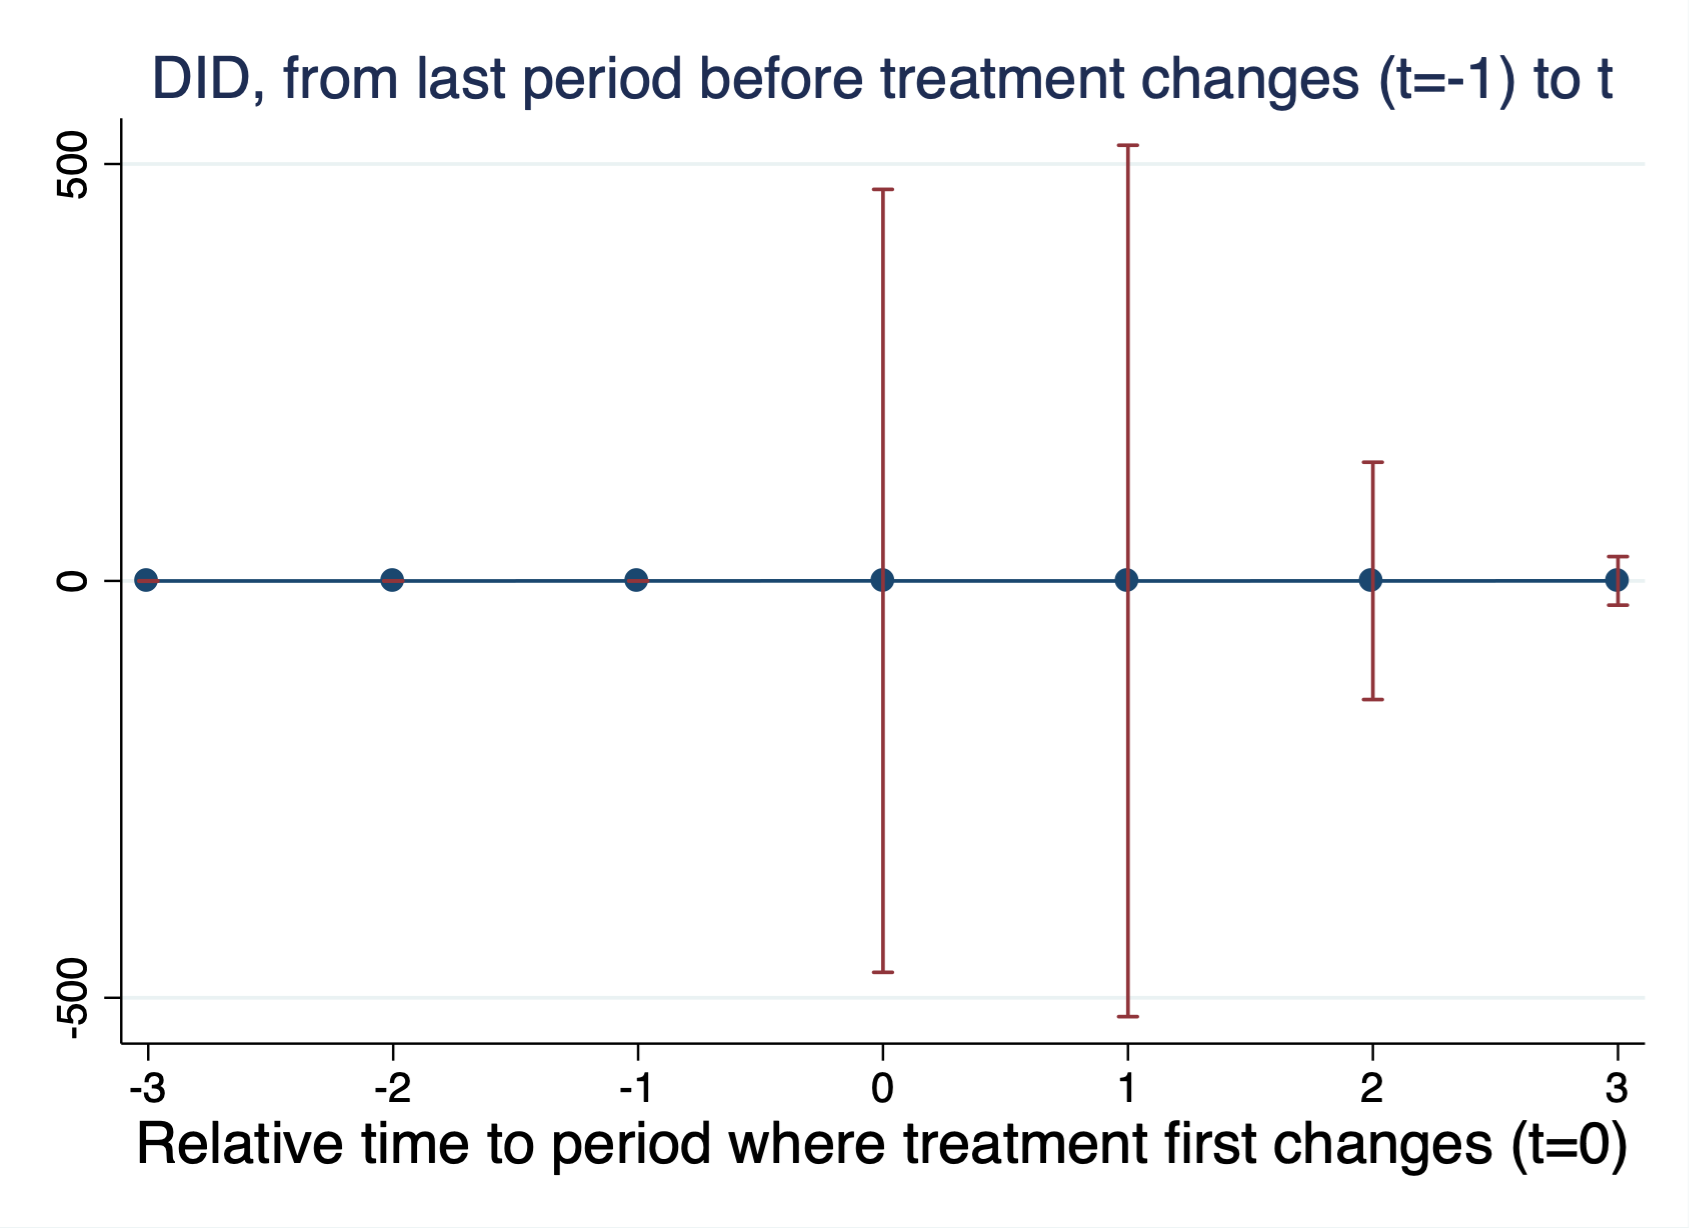
\includegraphics[width=0.9\textwidth]{Figures/chaisemartin_acuerdo_estcom.png}
       \captionsetup{justification=centering}
\end{figure}   

  %\begin{table}[htbp]\def\sym#1{\ifmmode^{#1}\else\(^{#1}\)\fi}
\centering
\caption{Comparison: Security Cooperation Agreements with Governor vs. Other Actors, 2014-2018}
\label{tab:as_comparison_agreements}
\scalebox{1}{
\begin{tabular}{lcc}
\hline \hline
\\ \multicolumn{3}{l}{Dependent variable: Security Cooperation Agreement}\\
& w/ Governor &  w/ Other Political Actors$^a$\\
& \multicolumn{1}{c}{(1)} & \multicolumn{1}{c}{(2)} \\
\cmidrule(lrr){2-2}  \cmidrule(lrr){3-3}\\
\addlinespace
Lag 4 years &         $ 0.0197^{} $ &      $ -0.0326^{} $  \\
& ($ 0.3292$) & ($ 0.0763 $) \\
Lag 3 years &        $ -0.0102^{***} $ &     $ 0.2193^{} $ \\
& ($ 0.0000$) & ($ 0.2702 $) \\
Lag 2 years &        $ 0.1418^{} $ &    $ -0.0648^{} $  \\
& ($ 0.1318$) & ($ 0.0524 $) \\
Reform, time 0 &        $ 0.0064^{} $ &     $ -0.0089^{} $ \\
& ($ 0.0354$) & ($ 0.0069 $) \\
Lead 1 year &         $ -0.2230^{***} $ &       $ -0.2858^{} $ \\
& ($ 0.0435$) & ($ 0.2610 $) \\
Lead 3 years &        $ -0.5921^{***} $ &     $ 0.1665^{} $ \\
& ($ 0.0708$) & ($ 0.1040 $) \\
\addlinespace
Observations       &                  4,382        &           4,382  \\
R-squared        &              0.6434        &           0.5469   \\
Mun. FEs       &     \checkmark         &  \checkmark    \\
Year. FEs       &     \checkmark         &  \checkmark   \\
Controls$^b$   &      \checkmark       &      \checkmark    \\
Cohort weighted   &   \checkmark       &   \checkmark    \\
WILD CI   &          &       \\
Aggregate effect        &              $-0.2696^{***} $$         &            $0.0796^{} $$   \\
SE (aggregate eff.)        &              (0.0339)       &           (0.0491)   \\
\hline \hline
\multicolumn{3}{p{0.7\textwidth}}{\footnotesize{Notes: Coefficients show IW estimators following \citet{abraham_sun_2020}. Two relative time periods (lag 5 and 1) are removed to avoid collinearity problems noted by \citet{abraham_sun_2020}. Standard errors in parentheses are clustered at the state level, with the following significance-level: $^{***}$ 1\%; $^{**}$ 5\%; and $^*$ 10\%, that refer to two-sided t-test with the null hypothesis equal to 0 for each relative time period. $^a$ Refers primarily to the President but could include Governors and mayors from other states or other municipalities from the same state. $^b$ Pretreatment controls include: governor winning margin; party alignment with the President;  party alignment with the Governor; municipal winning margin; logged population; logged organized crime related deaths; and Cartel presence.}} \\
\end{tabular}
}
\end{table}
   
  
  \begin{table}[htbp]\def\sym#1{\ifmmode^{#1}\else\(^{#1}\)\fi}
\centering
\caption{Effect of 2014 Term Limit Reform on the likelihood of signing Security Cooperation Agreements,  by type}
\label{tab:comparison_fed_estatal}
\scalebox{1}{
\begin{tabular}{lcccc}
\hline \hline
\\ \multicolumn{3}{l}{Dependent variable:}\\
& \multicolumn{2}{c}{Security Cooperation Agreement w/ Governor$^{a}$} & \multicolumn{2}{c}{Security Cooperation Agreement w/ Other$^{b}$} \\
& \multicolumn{1}{c}{(1)} & \multicolumn{1}{c}{(2)} & \multicolumn{1}{c}{(3)} & \multicolumn{1}{c}{(4)} \\
\cmidrule(lrr){2-3}  \cmidrule(lrr){4-5}\\
\addlinespace
t-4 &         $ 0.3497^{} $ &         $ 0.0193^{} $ &     $ -0.2763^{} $ &   $ -0.0326^{} $  \\
& ($ 1.8038$) & ($ 0.3316$) & ($ 0.5842$)  & ($ 0.0761 $) \\
t-3 &         $ -0.7355^{} $ &        $ -0.0102^{***} $  &     $ 0.2469^{} $ &     $ 0.2206^{} $ \\
& ($ 37.4159$) & ($ 0.0000$) & ($ 15.0281$) & ($ 0.2702 $) \\
t-2 &         $ 0.3861^{} $ &        $ 0.1420^{} $  &     $ -0.1496^{} $ &    $ -0.0649^{} $  \\
& ($ 0.3279$) & ($ 0.1323$) & ($ 0.1250$) & ($ 0.0524 $) \\
Reform (t=0) &         $ 0.2233^{***} $ &        $ 0.0065^{} $  &     $ -0.0599^{**} $  &     $ -0.0089^{} $ \\
& ($ 0.0581$) & ($ 0.0353$) & ($ 0.0273$) & ($ 0.0070 $) \\
t+1 &         $ -0.2198^{**} $ &         $ -0.2230^{***} $  &     $ 0.1148^{} $ &       $ -0.2845^{} $ \\
& ($ 0.0930$) & ($ 0.0435$) & ($ 0.0904$) & ($ 0.2602 $) \\
t+3 &         $ -0.5915^{***} $ &        $ -0.5921^{***} $ &     $ 0.1660^{*} $  &     $ 0.1665^{} $ \\
& ($ 0.0783$) & ($ 0.0708$) & ($ 0.0953$) & ($ 0.1040 $) \\
\addlinespace
Observations   &                  4,382     &                  4,382  &                  4,382        &           4,382  \\
R-squared      &              0.6433    &              0.6434   &            0.5469        &           0.5469   \\
Mun. FEs       &     \checkmark         &  \checkmark   &     \checkmark         &  \checkmark   \\
Year. FEs       &     \checkmark         &  \checkmark  &     \checkmark         &  \checkmark   \\
Controls$^b$   &      \checkmark       &      \checkmark   &      \checkmark       &      \checkmark   \\
Cohort weighted   &          &   \checkmark   &          &   \checkmark   \\
WILD CI  &     \checkmark         &  \checkmark   &     \checkmark         &  \checkmark   \\
Aggregate effect     &              $-0.213^{***} $$    &        $-0.2696^{***} $$      &            $0.069^{} $$   &       $0.0796^{} $$   \\
SE (aggregate eff.)      &              0.034   &              0.0339    &              0.045       &           0.0491   \\
\hline \hline
\multicolumn{5}{p{1.2\textwidth}}{\footnotesize{Notes: Coefficients in columns (2) and (4) show IW estimators following \citet{abraham_sun_2020}. In those models, two relative time periods (lag 8 and 1) are removed to avoid collinearity problems noted by \citet{abraham_sun_2020}. Standard errors in parentheses are clustered at the state level, with the following significance-level: $^{***}$ 1\%; $^{**}$ 5\%; and $^*$ 10\%, that refer to two-sided t-test with the null hypothesis equal to 0 for each relative time period. $^a$ Refers to security cooperation agreements signed with the governor only. $^b$ Refers to security cooperation agreements signed with other instituions but not the governor. $^c$ State-level controls include governor winning margin in last pre-treatment election and an indicator of whether the governor's party is the same as the federal incumbent party.}} \\
\end{tabular}
}
\end{table}
   
 
 
\def\sym#1{\ifmmode^{#1}\else\(^{#1}\)\fi}
\begin{table}[htbp]\def\sym#1{\ifmmode^{#1}\else\(^{#1}\)\fi}
\centering
\caption{Test on selection on unobservables}
\label{tab:unobservables}
\begin{tabular}{l*{1}{c}}
\hline \hline
&\multicolumn{1}{c}{(1)}         \\
\addlinespace
Fitted value&      0.1312         \\
            &    (0.0780)         \\
\addlinespace
Observations&      10,668         \\
R2          &       0.459         \\
Mun. FE     &      \checkmark               \\
Year FE     &      \checkmark               \\
State Cluster S.E.&     \checkmark                \\
\hline \hline 
\multicolumn{2}{p{0.6\textwidth}}{\footnotesize{Notes: I follow \citet{altonji_etal_2005} to check if unobserved variation is likely to explain the signing of security cooperation agreements with the Governor by mayors. To do so, I regress the treatment (whether the municipality held reelection) on all the available covariates used for Figure \ref{fig:event_study_agreements}.} I then take the fitted value from the regression and use it to predict each outcome, this time including unit and year fixed effects. This test suggests that – under the assumption that observables are representative of unobservables – selection on unobservables is not driving the results.} \\
\end{tabular}
\end{table} 

\clearpage 


\begin{comment}
\begin{figure}[H]
\centering
\caption{Effect of Electoral Reform on Security Cooperation Agreement using non parametric methods\\ -95\% confidence intervals-} 
\label{fig:non_did_agreement}
\begin{center} 
\begin{center} 
	{\textbf Figure A: Generalized Synthetic Control following \citet{xu_2016} }
\end{center}
\includegraphics[width=0.55\textwidth]{Figures/gsynth_wcov_acuerdo.png}

\begin{center}
	{\textbf Figure B: Matrix Completion following \citet{Athey, Bayati, Doudchenko, Imbens, and Khosvari}
\end{center}
\includegraphics[width=0.55\textwidth]{Figures/matrix_completion.png}
       \captionsetup{justification=centering}
       \\
 %{\textbf Note: 95\% confidence intervals estimated using 1,000 bootstrap replications.} .   
\end{figure}      
\end{comment}


\clearpage

\subsection{Mechanisms}

\begin{figure}[H] 
\centering
 \caption{Effect of 2014 Term Limit Reform on Motives to Sign Security Agreements w/ Governor}
 \label{fig:motives}
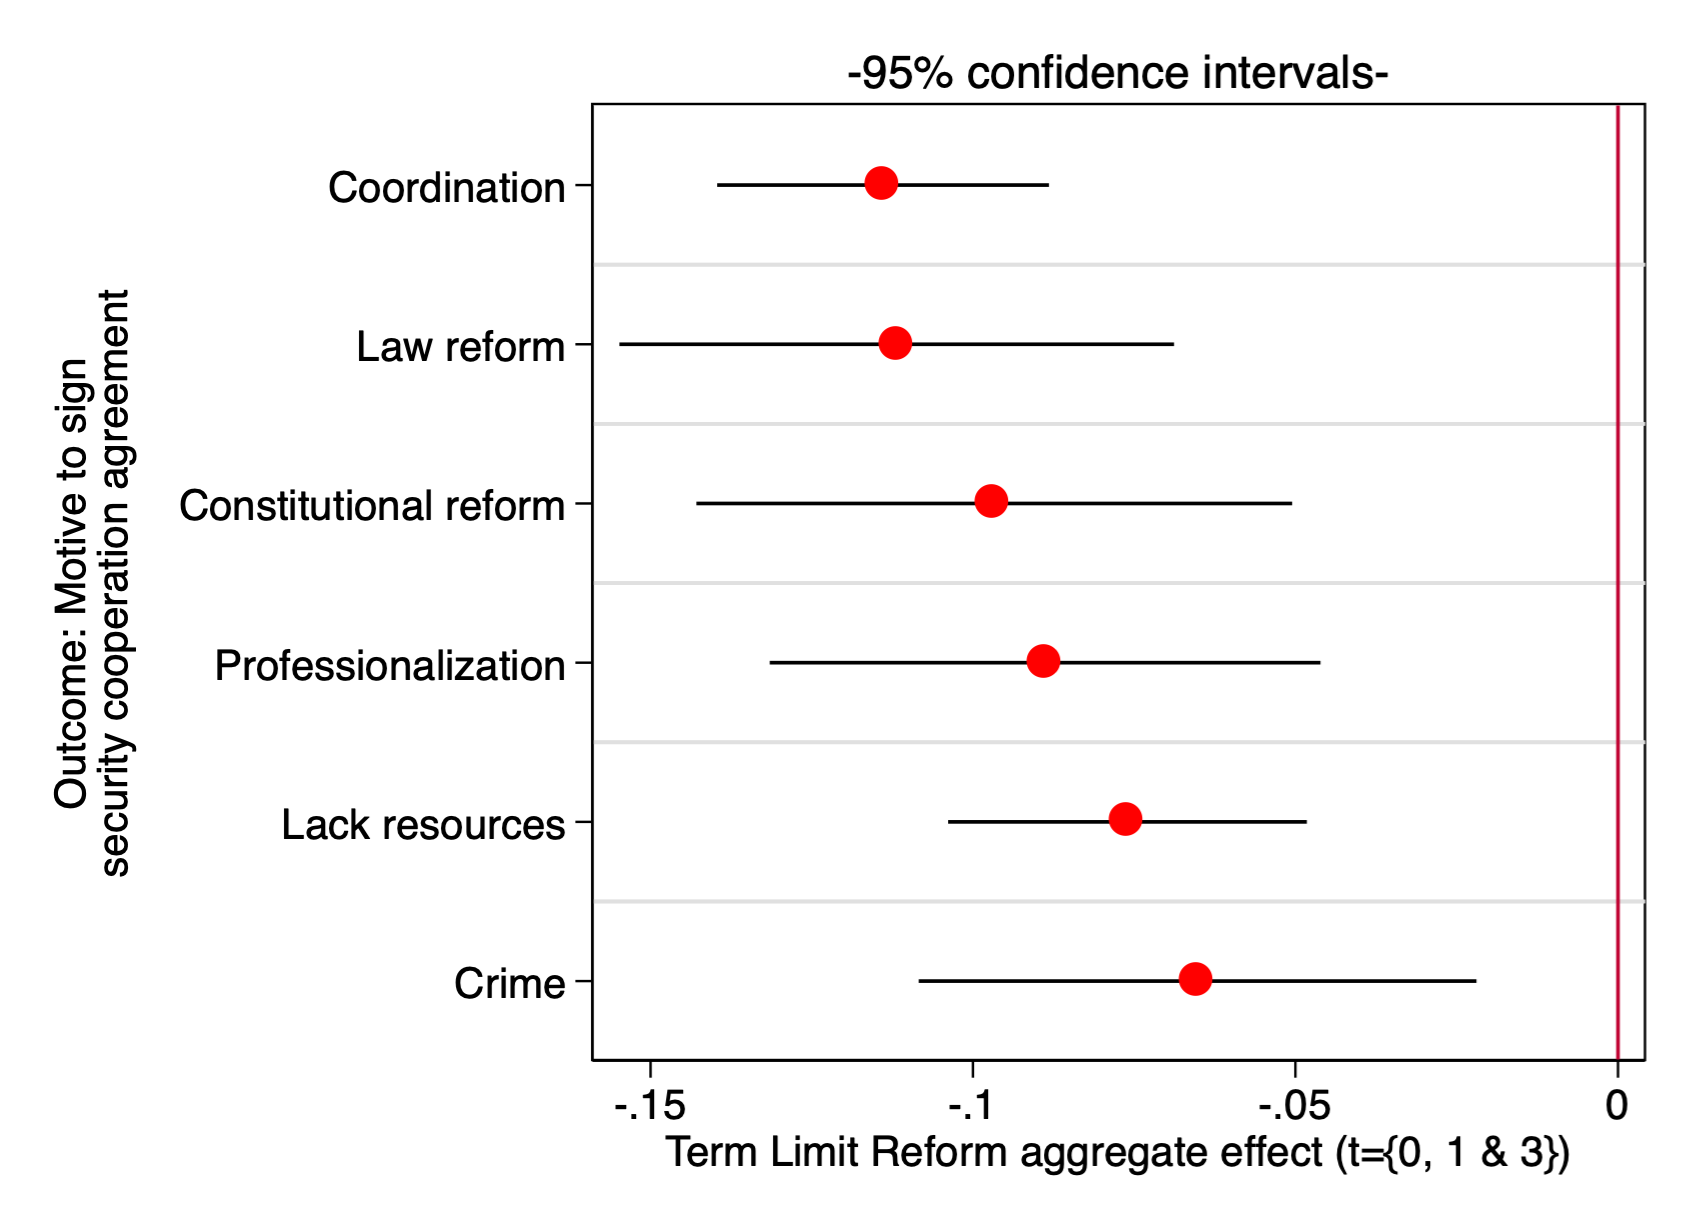
\includegraphics[width=0.9\textwidth]{Figures/motives.png}
       \captionsetup{justification=centering}
\end{figure}   

  \begin{landscape}
\begin{table}[htbp]\def\sym#1{\ifmmode^{#1}\else\(^{#1}\)\fi}
\centering
\caption{Effect of 2014 Term Limit Reform on Motives to Sign Security Agreements w/ Governor}
\label{tab:motives_final}
\scalebox{0.70}{
\begin{tabular}{lcccccc}
\hline \hline
\\ \multicolumn{7}{l}{Dependent variable:}\\
Motive: & Cons. reform  & Law reform & Lack resources & Professionalization & Coordination & Crime \\
& \multicolumn{1}{c}{(1)} & \multicolumn{1}{c}{(2)} & \multicolumn{1}{c}{(3)} & \multicolumn{1}{c}{(4)} & \multicolumn{1}{c}{(5)} & \multicolumn{1}{c}{(6)}  \\
\cmidrule(lrr){2-2}  \cmidrule(lrr){3-3} \cmidrule(lrr){4-4} \cmidrule(lrr){5-5} \cmidrule(lrr){6-6} \cmidrule(lrr){7-7} \\
\addlinespace
t-7 &     $ -0.2350^{***} $ &     $ -0.2581^{**} $ & $ -0.0955^{*} $ & $ -0.2000^{***} $  &     $ -0.1570^{*} $   &     $ -0.1538^{} $ \\
&     ($0.0407$) &     ($0.1175$) & ($0.0484$)& ($ 0.0671$)  &    ($0.0844$)   &   ($0.1078$) \\
t-6 &     $ -0.0758^{***} $ &     $ -0.0876^{***} $ &  $ -0.0615^{***} $ &  $ -0.0647^{} $  &     $ -0.0827^{**} $ &     $ -0.0369^{} $ \\
&     ($0.0176$) &     ($0.0199$) & ($0.0162$)& ($ 0.0585$)  &    ($0.0346$)   &   ($0.0265$) \\
t-5 &     $ 0.0223^{} $ &     $ -0.0405^{} $ &  $ 0.0574^{} $ &  $ 0.0580^{} $ &     $ -0.0106^{} $  &     $ 0.0427^{} $ \\
&     ($0.0591$) &     ($0.0583$) & ($0.0481$)& ($ 0.0750$)  &    ($0.0709$)   &   ($0.0445$) \\
t-4 &     $ 0.0167^{} $ &     $ -0.0832^{} $ &   $ 0.1207^{} $ &   $ 0.0649^{} $  &     $ -0.1313^{} $ &     $ 0.0346^{} $ \\
&     ($0.0987$) &     ($0.0842$) & ($0.0854$)& ($ 0.1053$)  &    ($0.2085$)   &   ($0.1173$) \\
t-3 &     $ -0.0385^{} $ &     $ -0.0160^{} $ &   $ 0.0727^{} $ &   $ 0.0802^{} $  &     $ 0.0403^{} $ &     $ 0.0734^{} $ \\
&     ($0.1052$) &     ($0.0840$) & ($0.1002$)& ($ 0.0738$)  &    ($0.1662$)   &   ($0.1061$) \\
t-2 &     $ -0.1162^{} $ &     $ -0.0914^{} $ &  $ 0.0228^{} $  &  $ -0.0822^{} $  &     $ -0.2796^{*} $ &     $ -0.0753^{} $ \\
&     ($0.1012$) &     ($0.0917$) & ($0.0640$)& ($ 0.1195$)  &    ($0.1379$)   &   ($0.0667$) \\
Reform (t=0) &     $ 0.0457^{} $ &     $ 0.0292^{} $ &   $ 0.0214^{} $   &   $ 0.0282^{} $  &     $ 0.0233^{} $ &     $ 0.0272^{*} $ \\
&     ($0.0278$) &     ($0.0183$) & ($0.0179$)& ($ 0.0201$)  &    ($0.0209$)   &   ($0.0146$) \\
t+1 &     $ -0.0906^{***} $ &     $ -0.1071^{***} $ &    $ -0.0935^{***} $ &    $ -0.0935^{***} $ &     $ -0.1215^{***} $ &     $ -0.0735^{***} $  \\
&     ($0.0164$) &     ($0.0182$) & ($0.0106$)& ($ 0.0160$)  &    ($0.0291$)   &   ($0.0121$) \\
t+3 &     $ -0.2452^{***} $ &     $ -0.2576^{***} $ &   $ -0.1560^{***} $  &   $ -0.2011^{***} $ &     $ -0.2436^{***} $ &     $ -0.1492^{***} $ \\
&     ($0.0535$) &     ($0.0484$) & ($0.0350$)& ($ 0.0463$)  &    ($0.0431$)   &   ($0.0527$) \\
\\
\addlinespace
Observations       &              9,725    &              9,725    &           9,725      &           9,725  &              9,725    &              9,725     \\
R-squared        &          0.2974 &          0.3021    &    0.2617       &           0.2722 &          0.2865 &          0.2594      \\
Mun. FEs      &     \checkmark         &  \checkmark   &     \checkmark         &  \checkmark  &     \checkmark         &  \checkmark   &     \checkmark         &  \checkmark   \\
Year. FEs    &     \checkmark         &  \checkmark   &     \checkmark         &  \checkmark &     \checkmark         &  \checkmark   &     \checkmark         &  \checkmark   \\
Controls$^b$  &    \checkmark     &       \checkmark  &    \checkmark      &   \checkmark &    \checkmark     &       \checkmark  &    \checkmark      &   \checkmark     \\
Cohort weighted  &   \checkmark      &       \checkmark  &   \checkmark       &   \checkmark  &   \checkmark      &       \checkmark  &   \checkmark       &   \checkmark    \\
Reform aggregate effect         & $-0.0967^{***} $$      & $-0.1118^{***} $$    & $-0.0760^{***} $$      & $-0.0888^{***} $$     & $-0.1139^{***} $$      & $-0.0652^{***} $$     \\
SE       & (0.0225)  & (0.0210) & (0.0136)  & (0.0208)  & (0.0125)  & (0.0211)   \\
\hline \hline
\multicolumn{7}{p{1.2\textwidth}}{\footnotesize{Notes: Coefficients show IW estimators following \citet{abraham_sun_2020}. Two relative time periods (lag 8 and 1) are removed to avoid collinearity problems noted by \citet{abraham_sun_2020}. Standard errors in parentheses are clustered at the state level for estimates in saturaded model. Significance-level: $^{***}$ 1\%; $^{**}$ 5\%; and $^*$ 10\%, that refer to two-sided t-test with the null hypothesis equal to 0 for each relative time period. $^a$ Even columns with outcomes with missing values where replaced by zeros assuming no activity was registered. $^b$ State-level controls include governor winning margin in last pre-treatment election and an indicator of whether the governor's party is the same as the federal incumbent party.}} \\
\end{tabular}
}
\end{table}
\end{landscape}
   

   %\begin{landscape}
\begin{table}[htbp]\def\sym#1{\ifmmode^{#1}\else\(^{#1}\)\fi}
\centering
\caption{Effect of 2014 Term Limit Reform on Motives to Sign Security Agreements w/ Governor}
\label{tab:motives_average_final}
\scalebox{0.70}{
\begin{tabular}{lcccccc}
\hline \hline
\\ \multicolumn{7}{l}{Dependent variable:}\\
Motive: & Cons. reform  & Law reform & Lack resources & Professionalization & Coordination & Crime \\
& \multicolumn{1}{c}{(1)} & \multicolumn{1}{c}{(2)} & \multicolumn{1}{c}{(3)} & \multicolumn{1}{c}{(4)} & \multicolumn{1}{c}{(5)} & \multicolumn{1}{c}{(6)}  \\
\cmidrule(lrr){2-2}  \cmidrule(lrr){3-3} \cmidrule(lrr){4-4} \cmidrule(lrr){5-5} \cmidrule(lrr){6-6} \cmidrule(lrr){7-7} \\
\addlinespace
Reform average effect         & $-0.0967^{***} $$      & $-0.1118^{***} $$     & $-0.0760^{***} $$        & $-0.0888^{***} $$       & $-0.1139^{***} $$        & $-0.0652^{***} $$       \\
& (0.0225)  & (0.0210) & (0.0136)  & (0.0208)  & (0.0125)  & (0.0211)   \\
\\
\addlinespace
Observations       &              9,725    &              9,725    &           9,725      &           9,725  &              9,725    &              9,725    \\
R-squared        &          0.2974 &          0.3021    &    0.2617       &           0.2722 &          0.2865 &          0.2594   \\
Mun. FEs      &     \checkmark         &  \checkmark   &     \checkmark         &  \checkmark  &     \checkmark         &  \checkmark   &     \checkmark         &  \checkmark   \\
Year. FEs    &     \checkmark         &  \checkmark   &     \checkmark         &  \checkmark &     \checkmark         &  \checkmark   &     \checkmark         &  \checkmark   \\
Controls$^b$  &    \checkmark     &       \checkmark  &    \checkmark      &   \checkmark &    \checkmark     &       \checkmark  &    \checkmark      &   \checkmark     \\
Cohort weighted  &   \checkmark      &       \checkmark  &   \checkmark       &   \checkmark  &   \checkmark      &       \checkmark  &   \checkmark       &   \checkmark    \\
Parallel trend holds &   \checkmark      &       \checkmark  &   \checkmark       &   \checkmark  &   \checkmark      &       \checkmark  &   \checkmark       &   \checkmark    \\
\hline \hline
\multicolumn{7}{p{1.2\textwidth}}{\footnotesize{Notes: Coefficients show IW estimators following \citet{abraham_sun_2020}. Two relative time periods (lag 8 and 1) are removed to avoid collinearity problems noted by \citet{abraham_sun_2020}. Standard errors in parentheses are clustered at the state level for estimates in saturaded model. Significance-level: $^{***}$ 1\%; $^{**}$ 5\%; and $^*$ 10\%, that refer to two-sided t-test with the null hypothesis equal to 0 for each relative time period. $^a$ Even columns with outcomes with missing values where replaced by zeros assuming no activity was registered. $^b$ State-level controls include governor winning margin in last pre-treatment election and an indicator of whether the governor's party is the same as the federal incumbent party.}} \\
\end{tabular}
}
\end{table}
\end{landscape}
  
   
   
      
\begin{landscape}
\begin{table}[htbp]\def\sym#1{\ifmmode^{#1}\else\(^{#1}\)\fi}
\centering
\caption{Effect of 2014 Term Limit Reform on Services Delegated to the Governor}
\label{tab:services}
\scalebox{0.70}{
\begin{tabular}{lcccccccc}
\hline \hline
\\ \multicolumn{9}{l}{Dependent variable:}\\
Service delegated: & Public security  & Traffic & Prevention & Training  & Technology & Research & Inteligence & Unify procedures \\
& \multicolumn{1}{c}{(1)} & \multicolumn{1}{c}{(2)} & \multicolumn{1}{c}{(3)} & \multicolumn{1}{c}{(4)} & \multicolumn{1}{c}{(5)} & \multicolumn{1}{c}{(6)} & \multicolumn{1}{c}{(7)} & \multicolumn{1}{c}{(8)} \\
\cmidrule(lrr){2-2}  \cmidrule(lrr){3-3} \cmidrule(lrr){4-4} \cmidrule(lrr){5-5} \cmidrule(lrr){6-6} \cmidrule(lrr){7-7} \cmidrule(lrr){8-8} \cmidrule(lrr){9-9} \\
\addlinespace
t-2 &     $ -0.0244^{} $ &     $ -0.0441^{} $ &  $ -0.0598^{***} $  &  $ -0.0565^{***} $  &     $ -0.0567^{***} $ &     $ -0.0596^{***} $ & $ -0.0596^{***} $ & $ -0.0506^{***} $   \\
&     ($0.1046$) &     ($0.0818$) & ($0.0021$)& ($ 0.0012$)  &    ($0.0016$)   &   ($0.0017$) \\
Reform (t=0) &     $ 0.0702^{} $ &     $ 0.0256^{} $ &   $ 0.0175^{} $   &   $ 0.0214^{} $  &     $ 0.0194^{} $ &     $ 0.0194^{} $ & $ 0.0204^{} $ & $ 0.0233^{} $   \\
&     ($0.0436$) &     ($0.0369$) & ($0.0137$)& ($ 0.0142$)  &    ($0.0126$)   &   ($0.0138$) \\
t+1 &     $ -0.0947^{*} $ &     $ -0.0259^{*} $ &    $ 0.0106^{} $ &    $ 0.0053^{} $ &     $ 0.0047^{} $ &     $ 0.0024^{} $  & $ 0.0018^{} $ & $ 0.0053^{} $   \\
&     ($0.0509$) &     ($0.0147$) & ($0.0198$)& ($ 0.0193$)  &    ($0.0197$)   &   ($0.0201$) \\
t+3 &     $ -0.2847^{***} $ &     $ 0.0000^{} $  \\
&     ($0.0430$) &     ($0.0000$)  \\
\\
\addlinespace
Observations       &              4,865    &              4,865    &           3,244      &           3,244  &              3,244    &              3,244  &              3,244    &              6,481   \\
R-squared        &          0.4234 &          0.3703    &    0.5567       &           0.5477 &          0.5409 &          0.5473     &        0.5467    &        0.4894   \\
Mun. FEs      &     \checkmark         &  \checkmark   &     \checkmark         &  \checkmark  &     \checkmark         &  \checkmark   &     \checkmark         &  \checkmark   \\
Year. FEs    &     \checkmark         &  \checkmark   &     \checkmark         &  \checkmark &     \checkmark         &  \checkmark   &     \checkmark         &  \checkmark   \\
Controls$^b$  &    \checkmark     &       \checkmark  &    \checkmark      &   \checkmark &    \checkmark     &       \checkmark  &    \checkmark      &   \checkmark     \\
Cohort weighted  &   \checkmark      &       \checkmark  &   \checkmark       &   \checkmark  &   \checkmark      &       \checkmark  &   \checkmark       &   \checkmark    \\
Reform average effect         & $-0.1031^{***} $$      & $-0.0242^{} $$     & $0.0094^{} $$        & $0.0133^{} $$       & $0.0121^{} $$        & $0.0109^{} $$    & $0.0111^{} $$      & $0.0143^{} $$     \\
SE (average effect)      & (0.0225)  & (0.0162) & (0.0080)  & (0.0120)  & (0.0117)  & (0.0122)    & (0.0123)  & (0.0114)   \\
\hline \hline
\multicolumn{9}{p{1.5\textwidth}}{\footnotesize{Notes: Coefficients show IW estimators following \citet{abraham_sun_2020}. Two relative time periods (lag 8 and 1) are removed to avoid collinearity problems noted by \citet{abraham_sun_2020}. Standard errors in parentheses are clustered at the state level for estimates in saturaded model. Significance-level: $^{***}$ 1\%; $^{**}$ 5\%; and $^*$ 10\%, that refer to two-sided t-test with the null hypothesis equal to 0 for each relative time period. $^a$ Even columns with outcomes with missing values where replaced by zeros assuming no activity was registered. $^b$ State-level controls include governor winning margin in last pre-treatment election and an indicator of whether the governor's party is the same as the federal incumbent party.}} \\
\end{tabular}
}
\end{table}
\end{landscape}
   
%\begin{landscape}
\begin{table}[htbp]\def\sym#1{\ifmmode^{#1}\else\(^{#1}\)\fi}
\centering
\caption{Effect of 2014 Term Limit Reform on Services Delegated to the Governor}
\label{tab:services_average}
\scalebox{0.70}{
\begin{tabular}{lcccccccc}
\hline \hline
\\ \multicolumn{9}{l}{Dependent variable:}\\
Service delegated: & Public security  & Traffic & Prevention & Training  & Technology & Research & Inteligence & Unify procedures \\
& \multicolumn{1}{c}{(1)} & \multicolumn{1}{c}{(2)} & \multicolumn{1}{c}{(3)} & \multicolumn{1}{c}{(4)} & \multicolumn{1}{c}{(5)} & \multicolumn{1}{c}{(6)} & \multicolumn{1}{c}{(7)} & \multicolumn{1}{c}{(8)} \\
\cmidrule(lrr){2-2}  \cmidrule(lrr){3-3} \cmidrule(lrr){4-4} \cmidrule(lrr){5-5} \cmidrule(lrr){6-6} \cmidrule(lrr){7-7} \cmidrule(lrr){8-8} \cmidrule(lrr){9-9} \\
\addlinespace
Reform average effect         & $0.0149^{*} $$      & $0.0579^{***} $$     & $0.0426^{***} $$        & $0.0034^{} $$       & $-0.0345^{***} $$        & $-0.0819^{***} $$    & $0.0092^{} $$      & $0.0056^{} $$     \\
SE       & (0.0079)  & (0.0099) & (0.0046)  & (0.0048)  & (0.0103)  & (0.0085)    & (0.0063)  & (0.0034)   \\
\addlinespace
Observations       &             11,353    &             11,353    &          11,353      &          11,353  &             11,353    &             11,353  &             11,353    &             11,353   \\
R-squared        &          0.8662 &          0.8556    &    0.9239       &           0.8767 &          0.8548 &          0.8954     &        0.8557    &        0.7008   \\
Mun. FEs      &     \checkmark         &  \checkmark   &     \checkmark         &  \checkmark  &     \checkmark         &  \checkmark   &     \checkmark         &  \checkmark   \\
Year. FEs    &     \checkmark         &  \checkmark   &     \checkmark         &  \checkmark &     \checkmark         &  \checkmark   &     \checkmark         &  \checkmark   \\
Controls$^b$  &    \checkmark     &       \checkmark  &    \checkmark      &   \checkmark &    \checkmark     &       \checkmark  &    \checkmark      &   \checkmark     \\
Cohort weighted  &   \checkmark      &       \checkmark  &   \checkmark       &   \checkmark  &   \checkmark      &       \checkmark  &   \checkmark       &   \checkmark    \\
Parallel trend holds &   \checkmark      &       \checkmark  &          &     &         &       &          &       \\
\hline \hline
\multicolumn{9}{p{1.5\textwidth}}{\footnotesize{Notes: Coefficients show IW estimators following \citet{abraham_sun_2020}. Two relative time periods (lag 8 and 1) are removed to avoid collinearity problems noted by \citet{abraham_sun_2020}. Standard errors in parentheses are clustered at the state level for estimates in saturaded model. Significance-level: $^{***}$ 1\%; $^{**}$ 5\%; and $^*$ 10\%, that refer to two-sided t-test with the null hypothesis equal to 0 for each relative time period. $^a$ Even columns with outcomes with missing values where replaced by zeros assuming no activity was registered. $^b$ State-level controls include governor winning margin in last pre-treatment election and an indicator of whether the governor's party is the same as the federal incumbent party.}} \\
\end{tabular}
}
\end{table}
\end{landscape}
   

\begin{landscape}
\begin{table}[htbp]\def\sym#1{\ifmmode^{#1}\else\(^{#1}\)\fi}
\centering
\caption{Effect of 2014 Term Limit Reform on Services Delegated to the Governor}
\label{tab:interaction_alignment}
\scalebox{0.70}{
\begin{tabular}{lccc}
\hline \hline
\\ \multicolumn{4}{l}{Dependent variable: Signing Security Cooperation Agreement w/ Governor}\\
Alignment: & w/ President  & w/ Governor  & w/ Governor from PRI \\
& \multicolumn{1}{c}{(1)} & \multicolumn{1}{c}{(2)} & \multicolumn{1}{c}{(3)} \\
\cmidrule(lrr){2-2}  \cmidrule(lrr){3-3} \cmidrule(lrr){4-4} \\
\addlinespace
t-7 &     $ -0.2383^{*} $ &     $ -0.0191^{*} $ &  $ 0.0000^{} $ \\
&     ($0.1348$) &     ($0.0108$) & ($0.0000$) \\
t-6 &     $ -0.0807^{} $ &     $ 0.0199^{} $ &  $ -0.0430^{} $  \\
&     ($0.0873$) &     ($0.0499$) & ($0.0467$) \\
t-5 &     $ -0.1186^{} $ &     $ -0.2028^{**} $ &  $ -0.2406^{**} $  \\
&     ($0.1046$) &     ($0.0924$) & ($0.0922$) \\
t-4 &     $ 0.0665^{} $ &     $ -0.0784^{} $ &  $ -0.1077^{} $  \\
&     ($0.1483$) &     ($0.1203$) & ($0.1236$) \\
t-3 &     $ 0.3395^{**} $ &     $ 0.2569^{***} $ &  $ 0.2303^{***} $  \\
&     ($0.1651$) &     ($0.0720$) & ($0.0702$) \\
t-2 &     $ 0.0027^{} $ &     $ -0.0253^{} $ &  $ 0.0976^{} $  \\
&     ($0.1572$) &     ($0.1182$) & ($0.1471$) \\
Reform (t=0) &     $ -0.1686^{} $ &     $ -0.2236^{} $ &   $ 0.1790^{} $   \\
&     ($0.1877$) &     ($0.1316$) & ($0.1258$) \\
t+1 &     $ -0.2169^{} $ &     $ -0.5692^{**} $ &    $ -0.0199^{} $ \\
&     ($0.1884$) &     ($0.2119$) & ($0.1549$) \\
t+2 &     $ -0.1125^{} $ &     $ -0.5020^{*} $  &     $ -0.4753^{*} $ \\
&     ($0.2496$) &     ($0.2690$)  & ($0.2741$) \\
t+3 &     $ -0.2197^{} $ &     $ -0.3562^{} $  &     $ -0.3876^{} $ \\
&     ($0.2241$) &     ($0.3827$)  & ($0.3818$) \\
\\
\addlinespace
Observations       &             12,173    &             12,173    &          12,173    \\
R-squared        &          0.4555 &          0.4566    &    0.4541    \\
Mun. FEs      &     \checkmark         &  \checkmark   &     \checkmark    \\
Year. FEs    &     \checkmark         &  \checkmark   &     \checkmark    \\
Controls$^b$  &    \checkmark     &       \checkmark  &    \checkmark   \\
Cohort weighted  &   \checkmark      &       \checkmark  &   \checkmark    \\
Reform average effect         & $-0.1376^{} $$      & $-0.1538^{*} $$     & $-0.0551^{} $$     \\
SE (average effect)      & (0.1313)  & (0.0906) & (0.0652) \\
\hline \hline
\multicolumn{4}{p{1.5\textwidth}}{\footnotesize{Notes: Coefficients show IW estimators following \citet{abraham_sun_2020}. Two relative time periods (lag 8 and 1) are removed to avoid collinearity problems noted by \citet{abraham_sun_2020}. Standard errors in parentheses are clustered at the state level for estimates in saturaded model. Significance-level: $^{***}$ 1\%; $^{**}$ 5\%; and $^*$ 10\%, that refer to two-sided t-test with the null hypothesis equal to 0 for each relative time period. $^a$ Even columns with outcomes with missing values where replaced by zeros assuming no activity was registered. $^b$ State-level controls include governor winning margin in last pre-treatment election and an indicator of whether the governor's party is the same as the federal incumbent party.}} \\
\end{tabular}
}
\end{table}
\end{landscape}
   
%\begin{landscape}
\begin{table}[htbp]\def\sym#1{\ifmmode^{#1}\else\(^{#1}\)\fi}
\centering
\caption{Effect of 2014 Term Limit Reform on Services Delegated to the Governor}
\label{tab:interaction_alignment_average}
\scalebox{0.70}{
\begin{tabular}{lccc}
\hline \hline
\\ \multicolumn{4}{l}{Dependent variable: Signing Security Cooperation Agreement w/ Governor}\\
Alignment: & w/ President  & w/ Governor  & w/ Governor from PRI \\
& \multicolumn{1}{c}{(1)} & \multicolumn{1}{c}{(2)} & \multicolumn{1}{c}{(3)} \\
\cmidrule(lrr){2-2}  \cmidrule(lrr){3-3} \cmidrule(lrr){4-4} \\
\addlinespace
Reform average effect         & $-0.1376^{} $$      & $-0.1538^{*} $$     & $-0.0551^{} $$     \\
& (0.1313)  & (0.0906) & (0.0652) \\
\\
\addlinespace
Observations       &             12,173    &             12,173    &          12,173    \\
R-squared        &          0.4555 &          0.4566    &    0.4541    \\
Mun. FEs      &     \checkmark         &  \checkmark   &     \checkmark    \\
Year. FEs    &     \checkmark         &  \checkmark   &     \checkmark    \\
Controls$^b$  &    \checkmark     &       \checkmark  &    \checkmark   \\
Cohort weighted  &   \checkmark      &       \checkmark  &   \checkmark    \\
\hline \hline
\multicolumn{4}{p{1.5\textwidth}}{\footnotesize{Notes: Coefficients show IW estimators following \citet{abraham_sun_2020}. Two relative time periods (lag 8 and 1) are removed to avoid collinearity problems noted by \citet{abraham_sun_2020}. Standard errors in parentheses are clustered at the state level for estimates in saturaded model. Significance-level: $^{***}$ 1\%; $^{**}$ 5\%; and $^*$ 10\%, that refer to two-sided t-test with the null hypothesis equal to 0 for each relative time period. $^a$ Even columns with outcomes with missing values where replaced by zeros assuming no activity was registered. $^b$ State-level controls include governor winning margin in last pre-treatment election and an indicator of whether the governor's party is the same as the federal incumbent party.}} \\
\end{tabular}
}
\end{table}
\end{landscape}
   

              
\begin{landscape}
\begin{table}[htbp]\def\sym#1{\ifmmode^{#1}\else\(^{#1}\)\fi}
\centering
\caption{Effect of 2014 Term Limit Reform on Services Delegated to the Governor}
\label{tab:interaction_trust}
\scalebox{0.70}{
\begin{tabular}{lcccccccc}
\hline \hline
\\ \multicolumn{9}{l}{Dependent variable: Signing Security Cooperation Agreement w/ Governor}\\
Jurisdiction: & \multicolumn{2}{c}{Municipal} & \multicolumn{2}{c}{State} & \multicolumn{4}{c}{Federal} \\
Police force: & Traffic  & Preventive  & State Police & State Attorney Police & Federal Police & Ministerial Police & Army & Marines \\
& \multicolumn{1}{c}{(1)} & \multicolumn{1}{c}{(2)} & \multicolumn{1}{c}{(3)} & \multicolumn{1}{c}{(4)} & \multicolumn{1}{c}{(5)} & \multicolumn{1}{c}{(6)} & \multicolumn{1}{c}{(7)} & \multicolumn{1}{c}{(8)} \\
\cmidrule(lrr){2-2}  \cmidrule(lrr){3-3} \cmidrule(lrr){4-4} \cmidrule(lrr){5-5} \cmidrule(lrr){6-6} \cmidrule(lrr){7-7} \cmidrule(lrr){8-8} \cmidrule(lrr){9-9} \\
\addlinespace
t-7 &     $ 0.1781^{} $ &     $ 0.0000^{} $ &  $ 0.1737^{} $  &  $ 0.1270^{} $  &     $ 0.0908^{} $ &     $ 0.1162^{} $ & $ 0.1093^{*} $ & $ 0.0788^{} $   \\
&     ($0.1657$) &     ($0.0000$) & ($0.1372$)& ($ 0.1137$)  &    ($0.0736$)   &   ($0.0858$) \\
t-6 &     $ -0.0459^{} $ &     $ -0.0601^{} $ &  $ -0.0414^{} $  &  $ -0.0565^{} $  &     $ 0.0055^{} $ &     $ -0.0537^{} $ & $ 0.0234^{} $ & $ 0.0038^{} $   \\
&     ($0.0801$) &     ($0.0481$) & ($0.0539$)& ($ 0.0457$)  &    ($0.0390$)   &   ($0.0379$) \\
t-5 &     $ -0.8924^{***} $ &     $ -0.2958^{} $ &  $ -0.7754^{} $  &  $ -1.3246^{} $  &     $ -0.8583^{**} $ &     $ -1.3844^{***} $ & $ -0.6699^{**} $ & $ -0.5789^{} $   \\
&     ($0.2538$) &     ($0.2470$) & ($0.6291$)& ($ 0.9127$)  &    ($0.3310$)   &   ($0.2853$) \\
t-4 &     $ -0.8387^{} $ &     $ -0.4847^{} $ &  $ -0.8341^{} $  &  $ -1.8134^{} $  &     $ -1.0918^{} $ &     $ -1.2394^{} $ & $ -0.3796^{} $ & $ -0.4926^{} $   \\
&     ($0.7688$) &     ($0.7827$) & ($0.7594$)& ($ 1.3210$)  &    ($0.7492$)   &   ($1.0419$) \\
t-3 &     $ -0.0581^{} $ &     $ -0.2251^{} $ &  $ -0.4852^{} $  &  $ -1.8471^{} $  &     $ -0.6960^{} $ &     $ -0.8290^{} $ & $ 0.1192^{} $ & $ -0.1124^{} $   \\
&     ($0.8135$) &     ($0.8597$) & ($0.7511$)& ($ 1.3390$)  &    ($0.8562$)   &   ($1.1144$) \\
t-2 &     $ 0.0341^{} $ &     $ -0.2671^{} $ &  $ -0.2891^{} $  &  $ -0.6196^{} $  &     $ -0.6138^{} $ &     $ -0.3468^{} $ & $ -0.4246^{} $ & $ -0.4023^{} $   \\
&     ($0.5384$) &     ($0.5922$) & ($0.4176$)& ($ 0.8966$)  &    ($0.4795$)   &   ($0.7851$) \\
Reform (t=0) &     $ -0.4444^{} $ &     $ 0.1161^{} $ &   $ -0.5432^{} $   &   $ -0.3590^{} $  &     $ -1.2942^{**} $ &     $ -0.8581^{} $ & $ -0.4514^{} $ & $ -0.8446^{} $   \\
&     ($0.4490$) &     ($0.4975$) & ($0.4116$)& ($ 1.1629$)  &    ($0.5674$)   &   ($0.7678$) \\
t+1 &     $ -0.9836^{} $ &     $ -0.2186^{} $ &    $ -1.3877^{**} $ &    $ -1.3449^{} $ &     $ -2.4941^{***} $ &     $ -1.8551^{*} $  & $ -1.5407^{**} $ & $ -1.8918^{**} $   \\
&     ($0.5947$) &     ($0.5769$) & ($0.6053$)& ($ 1.4393$)  &    ($0.7475$)   &   ($0.9449$) \\
t+2 &     $ -1.8506^{***} $ &     $ -1.6311^{**} $  \\
&     ($0.5938$) &     ($0.6871$)  \\
t+3 &     $ -0.1376^{} $ &     $ -1.5275^{} $  \\
&     ($1.1164$) &     ($1.1456$)  \\
\\
\addlinespace
Observations       &             12,173    &             12,173    &          12,173      &          12,173  &             12,173    &             12,173  &             12,173    &             12,173   \\
R-squared        &          0.4666 &          0.4641    &    0.4675       &           0.4673 &          0.4642 &          0.4719     &        0.4666    &        0.4666   \\
Mun. FEs      &     \checkmark         &  \checkmark   &     \checkmark         &  \checkmark  &     \checkmark         &  \checkmark   &     \checkmark         &  \checkmark   \\
Year. FEs    &     \checkmark         &  \checkmark   &     \checkmark         &  \checkmark &     \checkmark         &  \checkmark   &     \checkmark         &  \checkmark   \\
Controls$^b$  &    \checkmark     &       \checkmark  &    \checkmark      &   \checkmark &    \checkmark     &       \checkmark  &    \checkmark      &   \checkmark     \\
Cohort weighted  &   \checkmark      &       \checkmark  &   \checkmark       &   \checkmark  &   \checkmark      &       \checkmark  &   \checkmark       &   \checkmark    \\
Reform average effect         & $-0.1399^{} $$      & $-0.2053^{} $$     & $-0.3431^{**} $$        & $-0.2984^{**} $$       & $-0.5738^{**} $$        & $-0.2614^{**} $$    & $-0.4633^{} $$      & $-0.4835^{*} $$     \\
SE (average effect)      & (0.0944)  & (0.1633) & (0.1594)  & (0.1455)  & (0.2673)  & (0.1107)    & (0.4247)  & (0.2373)   \\
\hline \hline
\multicolumn{9}{p{1.5\textwidth}}{\footnotesize{Notes: Coefficients show IW estimators following \citet{abraham_sun_2020}. Two relative time periods (lag 8 and 1) are removed to avoid collinearity problems noted by \citet{abraham_sun_2020}. Standard errors in parentheses are clustered at the state level for estimates in saturaded model. Significance-level: $^{***}$ 1\%; $^{**}$ 5\%; and $^*$ 10\%, that refer to two-sided t-test with the null hypothesis equal to 0 for each relative time period. $^a$ Even columns with outcomes with missing values where replaced by zeros assuming no activity was registered. $^b$ State-level controls include governor winning margin in last pre-treatment election and an indicator of whether the governor's party is the same as the federal incumbent party.}} \\
\end{tabular}
}
\end{table}
\end{landscape}
   
%\begin{landscape}
\begin{table}[htbp]\def\sym#1{\ifmmode^{#1}\else\(^{#1}\)\fi}
\centering
\caption{Reform interaction with citizens' preferences}
\label{tab:interaction_trust_average}
\scalebox{0.70}{
\begin{tabular}{lcccccccc}
\hline \hline
\\ \multicolumn{9}{l}{Dependent variable: Signing Security Cooperation Agreement w/ Governor}\\
Jurisdiction: & \multicolumn{2}{c}{Municipal} & \multicolumn{2}{c}{State} & \multicolumn{4}{c}{Federal} \\
Trust in Police Force: & Traffic  & Preventive  & State Police & State Attorney Police & Federal Police & Ministerial Police & Army & Marines \\
& \multicolumn{1}{c}{(1)} & \multicolumn{1}{c}{(2)} & \multicolumn{1}{c}{(3)} & \multicolumn{1}{c}{(4)} & \multicolumn{1}{c}{(5)} & \multicolumn{1}{c}{(6)} & \multicolumn{1}{c}{(7)} & \multicolumn{1}{c}{(8)} \\
\cmidrule(lrr){2-2}  \cmidrule(lrr){3-3} \cmidrule(lrr){4-4} \cmidrule(lrr){5-5} \cmidrule(lrr){6-6} \cmidrule(lrr){7-7} \cmidrule(lrr){8-8} \cmidrule(lrr){9-9} \\
\addlinespace
Reform average effect         & $-0.1400^{} $$      & $-0.2053^{} $$     & $-0.3431^{**} $$        & $-0.2984^{**} $$       & $-0.5739^{**} $$        & $-0.2614^{**} $$    & $-0.4636^{} $$      & $-0.4837^{*} $$     \\
SE (average effect)      & (0.0944)  & (0.1633) & (0.1594)  & (0.1455)  & (0.2673)  & (0.1107)    & (0.4248)  & (0.2374)   \\
\\
\addlinespace
Observations       &             12,173    &             12,173    &          12,173      &          12,173  &             12,173    &             12,173  &             12,173    &             12,173   \\
R-squared        &          0.4666 &          0.4641    &    0.4675       &           0.4673 &          0.4642 &          0.4719     &        0.4666    &        0.4666   \\
Mun. FEs      &     \checkmark         &  \checkmark   &     \checkmark         &  \checkmark  &     \checkmark         &  \checkmark   &     \checkmark         &  \checkmark   \\
Year. FEs    &     \checkmark         &  \checkmark   &     \checkmark         &  \checkmark &     \checkmark         &  \checkmark   &     \checkmark         &  \checkmark   \\
Controls$^b$  &    \checkmark     &       \checkmark  &    \checkmark      &   \checkmark &    \checkmark     &       \checkmark  &    \checkmark      &   \checkmark     \\
Cohort weighted  &   \checkmark      &       \checkmark  &   \checkmark       &   \checkmark  &   \checkmark      &       \checkmark  &   \checkmark       &   \checkmark    \\
\hline \hline
\multicolumn{9}{p{1.5\textwidth}}{\footnotesize{Notes: Coefficients show IW estimators following \citet{abraham_sun_2020}. Two relative time periods (lag 8 and 1) are removed to avoid collinearity problems noted by \citet{abraham_sun_2020}. Standard errors in parentheses are clustered at the state level, with the following significance-level: $^{***}$ 1\%; $^{**}$ 5\%; and $^*$ 10\%, that refer to two-sided t-test with the null hypothesis equal to 0 for each relative time period. $^a$ Refers to security cooperation agreements signed with the Governor. $^b$ Pretreatment controls include: governor winning margin; party alignment with the President;  party alignment with the Governor; municipal winning margin; logged population; logged organized crime related deaths; and Cartel presence.}} \\
\end{tabular}
}
\end{table}
\end{landscape}
   
 
\begin{landscape}
\begin{table}[htbp]\def\sym#1{\ifmmode^{#1}\else\(^{#1}\)\fi}
\centering
\caption{Reform interaction with citizens' being able to identify a Police Force}
\label{tab:interaction_identify}
\scalebox{0.70}{
\begin{tabular}{lcccccccc}
\hline \hline
\\ \multicolumn{9}{l}{Dependent variable: Signing Security Cooperation Agreement w/ Governor}\\
Jurisdiction: & \multicolumn{2}{c}{Municipal} & \multicolumn{2}{c}{State} & \multicolumn{4}{c}{Federal} \\
Identify Policy Force: & Traffic  & Preventive  & State Police & State Attorney Police & Federal Police & Ministerial Police & Army & Marines \\
& \multicolumn{1}{c}{(1)} & \multicolumn{1}{c}{(2)} & \multicolumn{1}{c}{(3)} & \multicolumn{1}{c}{(4)} & \multicolumn{1}{c}{(5)} & \multicolumn{1}{c}{(6)} & \multicolumn{1}{c}{(7)} & \multicolumn{1}{c}{(8)} \\
\cmidrule(lrr){2-2}  \cmidrule(lrr){3-3} \cmidrule(lrr){4-4} \cmidrule(lrr){5-5} \cmidrule(lrr){6-6} \cmidrule(lrr){7-7} \cmidrule(lrr){8-8} \cmidrule(lrr){9-9} \\
\addlinespace
t-7 &     $ -0.8572^{} $ &     $ 0.1007^{} $ &  $ 0.0649^{} $  &  $ 0.0783^{} $  &     $ -2.5321^{***} $ &     $ 0.0632^{} $ & $ -1.4640^{*} $ & $ 0.0539^{} $   \\
&     ($0.6544$) &     ($0.0978$) & ($0.0611$)& ($ 0.0697$)  &    ($0.8962$)   &   ($0.0550$) &    ($0.8372$)   &   ($0.0455$) \\
t-6 &     $ -0.2641^{} $ &     $ 0.0248^{} $ &  $ 0.0135^{} $  &  $ 0.0056^{} $  &     $ -0.7692^{***} $ &     $ -0.0035^{} $ & $ -0.4466^{*} $ & $ 0.0092^{} $   \\
&     ($0.2039$) &     ($0.0609$) & ($0.0467$)& ($ 0.0441$)  &    ($0.2696$)   &   ($0.0413$) &    ($0.2577$)   &   ($0.0423$) \\
t-5 &     $ -0.4097^{} $ &     $ -0.0652^{} $ &  $ 0.6451^{} $  &  $ 0.1762^{} $  &     $ -1.1340^{**} $ &     $ -0.7691^{***} $ & $ -0.8805^{} $ & $ -0.3720^{} $   \\
&     ($0.3986$) &     ($0.3080$) & ($0.3960$)& ($ 0.4004$)  &    ($0.4306$)   &   ($0.2589$) &    ($0.5274$)   &   ($0.2421$) \\
t-4 &     $ 0.3350^{} $ &     $ 0.1050^{} $ &  $ 0.7461^{} $  &  $ -0.0893^{} $  &     $ -1.6040^{***} $ &     $ -0.2211^{} $ & $ -0.7589^{} $ & $ -0.3294^{} $   \\
&     ($0.5455$) &     ($0.5451$) & ($0.4774$)& ($ 0.6583$)  &    ($0.5716$)   &   ($0.7553$) &    ($0.8538$)   &   ($0.4995$) \\
t-3 &     $ 0.8549^{} $ &     $ 0.3354^{} $ &  $ 0.8618^{*} $  &  $ -0.1098^{} $  &     $ -1.2530^{**} $ &     $ 0.2973^{} $ & $ -0.3261^{} $ & $ -0.0407^{} $   \\
&     ($0.5572$) &     ($0.6384$) & ($0.5038$)& ($ 0.7313$)  &    ($0.6065$)   &   ($0.8187$) &    ($0.8829$)   &   ($0.5638$) \\
t-2 &     $ -0.0741^{} $ &     $ 0.0173^{} $ &  $ 0.3106^{} $  &  $ -0.0035^{} $  &     $ -1.1572^{**} $ &     $ -0.2290^{} $ & $ -0.7416^{} $ & $ -0.3552^{} $   \\
&     ($0.3985$) &     ($0.3426$) & ($0.3583$)& ($ 0.4741$)  &    ($0.4705$)   &   ($0.5458$) &    ($0.5501$)   &   ($0.3444$) \\
Reform (t=0) &     $ 0.0965^{} $ &     $ -0.3095^{} $ &   $ -0.6740^{} $   &   $ -0.0176^{} $  &     $ -1.7122^{***} $ &     $ -0.3017^{} $ & $ -0.8230^{} $ & $ -0.7614^{} $   \\
&     ($0.3746$) &     ($0.5580$) & ($0.5072$)& ($ 0.5448$)  &    ($0.5196$)   &   ($0.5185$) &    ($0.5125$)   &   ($0.4724$) \\
t+1 &     $ 0.1452^{} $ &     $ -0.8415^{} $ &    $ -0.5733^{} $ &    $ -0.5894^{} $ &     $ -1.1449^{**} $ &     $ -1.2316^{} $  & $ -0.8753^{} $ & $ -1.6442^{***} $   \\
&     ($0.4015$) &     ($0.7920$) & ($0.6386$)& ($ 0.7035$)  &    ($0.4877$)   &   ($0.7296$) &    ($0.5560$)   &   ($0.5433$) \\
t+2 &     $ 0.4499^{} $ &     $ -0.7212^{} $ &    $ 0.0862^{} $ &    $ -1.4956^{**} $ &     $ -0.5687^{} $ &     $ -1.6626^{**} $  & $ -0.4091^{} $ & $ -1.5000^{**} $   \\
&     ($0.3760$) &     ($0.7799$) & ($0.6272$)& ($ 0.7215$)  &    ($0.5955$)   &   ($0.6266$) &    ($0.6311$)   &   ($0.5652$) \\
t+3 &     $ 1.1277^{} $ &     $ -0.5739^{} $ &    $ -0.6702^{} $ &    $ -1.2519^{} $ &     $ -1.7933^{} $ &     $ 0.0623^{} $  & $ -0.5981^{} $ & $ -1.0885^{} $   \\
&     ($0.9218$) &     ($1.2931$) & ($0.9352$)& ($ 1.0598$)  &    ($1.0758$)   &   ($1.0916$) &    ($0.9325$)   &   ($0.9434$) \\
\\
\addlinespace
Observations       &             12,173    &             12,173    &          12,173      &          12,173  &             12,173    &             12,173  &             12,173    &             12,173   \\
R-squared        &          0.4688 &          0.4599    &    0.4659       &           0.4658 &          0.4624 &          0.4783     &        0.4645    &        0.4655   \\
Mun. FEs      &     \checkmark         &  \checkmark   &     \checkmark         &  \checkmark  &     \checkmark         &  \checkmark   &     \checkmark         &  \checkmark   \\
Year. FEs    &     \checkmark         &  \checkmark   &     \checkmark         &  \checkmark &     \checkmark         &  \checkmark   &     \checkmark         &  \checkmark   \\
Controls$^b$  &    \checkmark     &       \checkmark  &    \checkmark      &   \checkmark &    \checkmark     &       \checkmark  &    \checkmark      &   \checkmark     \\
Cohort weighted  &   \checkmark      &       \checkmark  &   \checkmark       &   \checkmark  &   \checkmark      &       \checkmark  &   \checkmark       &   \checkmark    \\
Reform average effect         & $0.3037^{} $      & $-0.4471^{} $     & $-0.2964^{} $        & $-0.3087^{} $       & $-0.7782^{**} $        & $-0.2768^{} $    & $-0.5017^{} $      & $-0.5781^{**} $     \\
SE (average effect)      & (0.3233)  & (0.6044) & (0.3716)  & (0.2401)  & (0.2868)  & (0.2411)    & (0.4665)  & (0.2669)   \\
\hline \hline
\multicolumn{9}{p{1.6\textwidth}}{\footnotesize{Notes: Coefficients show IW estimators following \citet{abraham_sun_2020}. Two relative time periods (lag 8 and 1) are removed to avoid collinearity problems noted by \citet{abraham_sun_2020}. Standard errors in parentheses are clustered at the state level, with the following significance-level: $^{***}$ 1\%; $^{**}$ 5\%; and $^*$ 10\%, that refer to two-sided t-test with the null hypothesis equal to 0 for each relative time period. $^a$ Refers to security cooperation agreements signed with the Governor. $^b$ Pretreatment controls include: governor winning margin; party alignment with the President;  party alignment with the Governor; municipal winning margin; logged population; logged organized crime related deaths; and Cartel presence.}} \\
\end{tabular}
}
\end{table}
\end{landscape}
   
%\begin{landscape}
\begin{table}[htbp]\def\sym#1{\ifmmode^{#1}\else\(^{#1}\)\fi}
\centering
\caption{Reform interaction with citizens' being able to identify a Police Force}
\label{tab:interaction_identify_average}
\scalebox{0.70}{
\begin{tabular}{lcccccccc}
\hline \hline
\\ \multicolumn{9}{l}{Dependent variable: Signing Security Cooperation Agreement w/ Governor}\\
Jurisdiction: & \multicolumn{2}{c}{Municipal} & \multicolumn{2}{c}{State} & \multicolumn{4}{c}{Federal} \\
Identify Policy Force: & Traffic  & Preventive  & State Police & State Attorney Police & Federal Police & Ministerial Police & Army & Marines \\
& \multicolumn{1}{c}{(1)} & \multicolumn{1}{c}{(2)} & \multicolumn{1}{c}{(3)} & \multicolumn{1}{c}{(4)} & \multicolumn{1}{c}{(5)} & \multicolumn{1}{c}{(6)} & \multicolumn{1}{c}{(7)} & \multicolumn{1}{c}{(8)} \\
\cmidrule(lrr){2-2}  \cmidrule(lrr){3-3} \cmidrule(lrr){4-4} \cmidrule(lrr){5-5} \cmidrule(lrr){6-6} \cmidrule(lrr){7-7} \cmidrule(lrr){8-8} \cmidrule(lrr){9-9} \\
\addlinespace
Reform average effect         & $0.3037^{} $$      & $-0.4471^{} $$     & $-0.2964^{} $$        & $-0.3087^{} $$       & $-0.7782^{**} $$        & $-0.2768^{} $$    & $-0.5017^{} $$      & $-0.5781^{**} $$     \\
SE (average effect)      & (0.3233)  & (0.6044) & (0.3716)  & (0.2401)  & (0.2868)  & (0.2411)    & (0.4665)  & (0.2669)   \\
\\
\addlinespace
Observations       &             12,173    &             12,173    &          12,173      &          12,173  &             12,173    &             12,173  &             12,173    &             12,173   \\
R-squared        &          0.4688 &          0.4599    &    0.4659       &           0.4658 &          0.4624 &          0.4783     &        0.4645    &        0.4655   \\
Mun. FEs      &     \checkmark         &  \checkmark   &     \checkmark         &  \checkmark  &     \checkmark         &  \checkmark   &     \checkmark         &  \checkmark   \\
Year. FEs    &     \checkmark         &  \checkmark   &     \checkmark         &  \checkmark &     \checkmark         &  \checkmark   &     \checkmark         &  \checkmark   \\
Controls$^b$  &    \checkmark     &       \checkmark  &    \checkmark      &   \checkmark &    \checkmark     &       \checkmark  &    \checkmark      &   \checkmark     \\
Cohort weighted  &   \checkmark      &       \checkmark  &   \checkmark       &   \checkmark  &   \checkmark      &       \checkmark  &   \checkmark       &   \checkmark    \\
\hline \hline
\multicolumn{9}{p{1.6\textwidth}}{\footnotesize{Notes: Coefficients show IW estimators following \citet{abraham_sun_2020}. Two relative time periods (lag 8 and 1) are removed to avoid collinearity problems noted by \citet{abraham_sun_2020}. Standard errors in parentheses are clustered at the state level, with the following significance-level: $^{***}$ 1\%; $^{**}$ 5\%; and $^*$ 10\%, that refer to two-sided t-test with the null hypothesis equal to 0 for each relative time period. $^a$ Refers to security cooperation agreements signed with the Governor. $^b$ Pretreatment controls include: governor winning margin; party alignment with the President;  party alignment with the Governor; municipal winning margin; logged population; logged organized crime related deaths; and Cartel presence.}} \\
\end{tabular}
}
\end{table}
\end{landscape}
   
  
 \begin{landscape}
\begin{table}[htbp]\def\sym#1{\ifmmode^{#1}\else\(^{#1}\)\fi}
\centering
\caption{Reform interaction with citizens' efficiency evaluation of police forces}
\label{tab:interaction_identify}
\scalebox{0.70}{
\begin{tabular}{lcccccccc}
\hline \hline
\\ \multicolumn{9}{l}{Dependent variable: Signing Security Cooperation Agreement w/ Governor}\\
Jurisdiction: & \multicolumn{2}{c}{Municipal} & \multicolumn{2}{c}{State} & \multicolumn{4}{c}{Federal} \\
Efficiency Policy Force: & Traffic  & Preventive  & State Police & State Attorney Police & Federal Police & Ministerial Police & Army & Marines \\
& \multicolumn{1}{c}{(1)} & \multicolumn{1}{c}{(2)} & \multicolumn{1}{c}{(3)} & \multicolumn{1}{c}{(4)} & \multicolumn{1}{c}{(5)} & \multicolumn{1}{c}{(6)} & \multicolumn{1}{c}{(7)} & \multicolumn{1}{c}{(8)} \\
\cmidrule(lrr){2-2}  \cmidrule(lrr){3-3} \cmidrule(lrr){4-4} \cmidrule(lrr){5-5} \cmidrule(lrr){6-6} \cmidrule(lrr){7-7} \cmidrule(lrr){8-8} \cmidrule(lrr){9-9} \\
\addlinespace
t-7 &     $ 0.1495^{} $ &     $ 0.0000^{} $ &  $ 0.1580^{} $  &  $ 0.1178^{} $  &     $ 0.0821^{} $ &     $ 0.1125^{} $ & $ 0.0996^{} $ & $ 0.0723^{} $   \\
&     ($0.1280$) &     ($0.0000$) & ($0.1237$)& ($ 0.1059$)  &    ($0.0677$)   &   ($0.0823$) &    ($0.0592$)   &   ($0.0533$) \\
t-6 &     $ -0.0430^{} $ &     $ -0.0600^{} $ &  $ -0.0408^{} $  &  $ -0.0550^{} $  &     $ 0.0050^{} $ &     $ -0.0539^{} $ & $ 0.0218^{} $ & $ 0.0031^{} $   \\
&     ($0.0554$) &     ($0.0481$) & ($0.0487$)& ($ 0.0432$)  &    ($0.0413$)   &   ($0.0372$) &    ($0.0432$)   &   ($0.0431$) \\
t-5 &     $ -0.8214^{***} $ &     $ -0.2661^{} $ &  $ -0.6765^{} $  &  $ -1.0574^{} $  &     $ -0.8511^{**} $ &     $ -1.3151^{***} $ & $ -0.6265^{*} $ & $ -0.5477^{} $   \\
&     ($0.2173$) &     ($0.2280$) & ($0.5991$)& ($ 0.8293$)  &    ($0.3265$)   &   ($0.2946$) &    ($0.3331$)   &   ($0.3312$) \\
t-4 &     $ -0.5218^{} $ &     $ -0.3094^{} $ &  $ -0.6839^{} $  &  $ -1.4607^{} $  &     $ -1.0699^{} $ &     $ -1.1764^{} $ & $ -0.3632^{} $ & $ -0.4794^{} $   \\
&     ($0.6322$) &     ($0.6711$) & ($0.7109$)& ($ 1.2102$)  &    ($0.6659$)   &   ($0.9647$) &    ($0.5751$)   &   ($0.6316$) \\
t-3 &     $ 0.1534^{} $ &     $ -0.0826^{} $ &  $ -0.3839^{} $  &  $ -1.5521^{} $  &     $ -0.6947^{} $ &     $ -0.7613^{} $ & $ 0.1118^{} $ & $ -0.1206^{} $   \\
&     ($0.6633$) &     ($0.7380$) & ($0.6994$)& ($ 1.2330$)  &    ($0.7686$)   &   ($1.0338$) &    ($0.6450$)   &   ($0.6843$) \\
t-2 &     $ 0.1301^{} $ &     $ -0.1088^{} $ &  $ -0.2605^{} $  &  $ -0.4476^{} $  &     $ -0.6274^{} $ &     $ -0.3362^{} $ & $ -0.4306^{} $ & $ -0.4001^{} $   \\
&     ($0.4219$) &     ($0.5170$) & ($0.3883$)& ($ 0.8207$)  &    ($0.4341$)   &   ($0.7275$) &    ($0.3376$)   &   ($0.4258$) \\
Reform (t=0) &     $ -0.2825^{} $ &     $ 0.2132^{} $ &   $ -0.4068^{} $   &   $ -0.1690^{} $  &     $ -1.2332^{**} $ &     $ -0.6252^{} $ & $ -0.4515^{} $ & $ -0.8273^{} $   \\
&     ($0.3771$) &     ($0.4424$) & ($0.3661$)& ($ 1.0199$)  &    ($0.5445$)   &   ($0.7224$) &    ($0.4956$)   &   ($0.5171$) \\
t+1 &     $ -0.8544^{} $ &     $ -0.1639^{} $ &    $ -1.2047^{**} $ &    $ -1.0867^{} $ &     $ -2.4180^{***} $ &     $ -1.5837^{*} $  & $ -1.5141^{**} $ & $ -1.8447^{***} $   \\
&     ($0.5069$) &     ($0.5180$) & ($0.5515$)& ($ 1.2521$)  &    ($0.7203$)   &   ($0.9025$) &    ($0.7243$)   &   ($0.6586$) \\
t+2 &     $ -1.6548^{***} $ &     $ -1.5020^{**} $ &    $ -1.7252^{**} $ &    $ -3.6912^{***} $ &     $ -2.2110^{***} $ &     $ -3.0680^{***} $  & $ -1.1837^{} $ & $ -1.7816^{**} $   \\
&     ($0.5166$) &     ($0.6272$) & ($0.8167$)& ($ 1.0720$)  &    ($0.7669$)   &   ($0.6529$) &    ($0.7910$)   &   ($0.6492$) \\
t+3 &     $ -0.0738^{} $ &     $ -1.2495^{} $ &    $ -0.8880^{} $ &    $ -1.8369^{*} $ &     $ -1.0878^{} $ &     $ -1.0650^{} $  & $ -0.0721^{} $ & $ -1.0091^{} $   \\
&     ($0.9252$) &     ($1.0025$) & ($0.7675$)& ($ 1.0415$)  &    ($1.3469$)   &   ($1.1792$) &    ($1.2083$)   &   ($1.0552$) \\
\\
\addlinespace
Observations       &             12,173    &             12,173    &          12,173      &          12,173  &             12,173    &             12,173  &             12,173    &             12,173   \\
R-squared        &          0.4692 &          0.4656    &    0.4672       &           0.4675 &          0.4642 &          0.4725     &        0.4667    &        0.4667   \\
Mun. FEs      &     \checkmark         &  \checkmark   &     \checkmark         &  \checkmark  &     \checkmark         &  \checkmark   &     \checkmark         &  \checkmark   \\
Year. FEs    &     \checkmark         &  \checkmark   &     \checkmark         &  \checkmark &     \checkmark         &  \checkmark   &     \checkmark         &  \checkmark   \\
Controls$^b$  &    \checkmark     &       \checkmark  &    \checkmark      &   \checkmark &    \checkmark     &       \checkmark  &    \checkmark      &   \checkmark     \\
Cohort weighted  &   \checkmark      &       \checkmark  &   \checkmark       &   \checkmark  &   \checkmark      &       \checkmark  &   \checkmark       &   \checkmark    \\
Reform average effect         & $-0.1373^{} $      & $-0.1957^{} $     & $-0.3432^{*} $        & $-0.2914^{*} $       & $-0.6190^{**} $        & $-0.2679^{**} $    & $-0.5001^{} $      & $-0.5024^{**} $     \\
SE (average effect)      & (0.0917)  & (0.1697) & (0.1707)  & (0.1453)  & (0.2769)  & (0.1215)    & (0.4693)  & (0.2369)   \\
\hline \hline
\multicolumn{9}{p{1.6\textwidth}}{\footnotesize{Notes: Coefficients show IW estimators following \citet{abraham_sun_2020}. Two relative time periods (lag 8 and 1) are removed to avoid collinearity problems noted by \citet{abraham_sun_2020}. Standard errors in parentheses are clustered at the state level, with the following significance-level: $^{***}$ 1\%; $^{**}$ 5\%; and $^*$ 10\%, that refer to two-sided t-test with the null hypothesis equal to 0 for each relative time period. $^a$ Refers to security cooperation agreements signed with the Governor. $^b$ Pretreatment controls include: governor winning margin; party alignment with the President;  party alignment with the Governor; municipal winning margin; logged population; logged organized crime related deaths; and Cartel presence.}} \\
\end{tabular}
}
\end{table}
\end{landscape}
   
%\begin{landscape}
\begin{table}[htbp]\def\sym#1{\ifmmode^{#1}\else\(^{#1}\)\fi}
\centering
\caption{Effect of 2014 Term Limit Reform on Services Delegated to the Governor}
\label{tab:interaction_performance_average}
\scalebox{0.70}{
\begin{tabular}{lcccccccc}
\hline \hline
\\ \multicolumn{9}{l}{Dependent variable: Signing Security Cooperation Agreement w/ Governor}\\
Jurisdiction: & \multicolumn{2}{c}{Municipal} & \multicolumn{2}{c}{State} & \multicolumn{4}{c}{Federal} \\
Police force: & Traffic  & Preventive  & State Police & State Attorney Police & Federal Police & Ministerial Police & Army & Marines \\
& \multicolumn{1}{c}{(1)} & \multicolumn{1}{c}{(2)} & \multicolumn{1}{c}{(3)} & \multicolumn{1}{c}{(4)} & \multicolumn{1}{c}{(5)} & \multicolumn{1}{c}{(6)} & \multicolumn{1}{c}{(7)} & \multicolumn{1}{c}{(8)} \\
\cmidrule(lrr){2-2}  \cmidrule(lrr){3-3} \cmidrule(lrr){4-4} \cmidrule(lrr){5-5} \cmidrule(lrr){6-6} \cmidrule(lrr){7-7} \cmidrule(lrr){8-8} \cmidrule(lrr){9-9} \\
\addlinespace
Reform average effect         & $-0.1373^{} $$      & $-0.1957^{} $$     & $-0.3431^{*} $$        & $-0.2913^{*} $$       & $-0.6189^{**} $$        & $-0.2678^{**} $$    & $-0.4999^{} $$      & $-0.5022^{**} $$     \\
SE (average effect)      & (0.0917)  & (0.1697) & (0.1706)  & (0.1453)  & (0.2768)  & (0.1215)    & (0.4692)  & (0.2369)   \\
\\
\addlinespace
Observations       &             12,173    &             12,173    &          12,173      &          12,173  &             12,173    &             12,173  &             12,173    &             12,173   \\
R-squared        &          0.4692 &          0.4656    &    0.4672       &           0.4675 &          0.4642 &          0.4725     &        0.4667    &        0.4667   \\
Mun. FEs      &     \checkmark         &  \checkmark   &     \checkmark         &  \checkmark  &     \checkmark         &  \checkmark   &     \checkmark         &  \checkmark   \\
Year. FEs    &     \checkmark         &  \checkmark   &     \checkmark         &  \checkmark &     \checkmark         &  \checkmark   &     \checkmark         &  \checkmark   \\
Controls$^b$  &    \checkmark     &       \checkmark  &    \checkmark      &   \checkmark &    \checkmark     &       \checkmark  &    \checkmark      &   \checkmark     \\
Cohort weighted  &   \checkmark      &       \checkmark  &   \checkmark       &   \checkmark  &   \checkmark      &       \checkmark  &   \checkmark       &   \checkmark    \\
\hline \hline
\multicolumn{9}{p{1.5\textwidth}}{\footnotesize{Notes: Coefficients show IW estimators following \citet{abraham_sun_2020}. Two relative time periods (lag 8 and 1) are removed to avoid collinearity problems noted by \citet{abraham_sun_2020}. Standard errors in parentheses are clustered at the state level for estimates in saturaded model. Significance-level: $^{***}$ 1\%; $^{**}$ 5\%; and $^*$ 10\%, that refer to two-sided t-test with the null hypothesis equal to 0 for each relative time period. $^a$ Even columns with outcomes with missing values where replaced by zeros assuming no activity was registered. $^b$ State-level controls include governor winning margin in last pre-treatment election and an indicator of whether the governor's party is the same as the federal incumbent party.}} \\
\end{tabular}
}
\end{table}
\end{landscape}
 
  
  \begin{landscape}
\begin{table}[htbp]\def\sym#1{\ifmmode^{#1}\else\(^{#1}\)\fi}
\centering
\caption{Reform interaction with citizens' corruption evaluation of police forces}
\label{tab:interaction_corrupt}
\scalebox{0.70}{
\begin{tabular}{lcccccccc}
\hline \hline
\\ \multicolumn{9}{l}{Dependent variable: Signing Security Cooperation Agreement w/ Governor}\\
Jurisdiction: & \multicolumn{2}{c}{Municipal} & \multicolumn{2}{c}{State} & \multicolumn{4}{c}{Federal} \\
Corruption of Police Forces: & Traffic  & Preventive  & State Police & State Attorney Police & Federal Police & Ministerial Police & Army & Marines \\
& \multicolumn{1}{c}{(1)} & \multicolumn{1}{c}{(2)} & \multicolumn{1}{c}{(3)} & \multicolumn{1}{c}{(4)} & \multicolumn{1}{c}{(5)} & \multicolumn{1}{c}{(6)} & \multicolumn{1}{c}{(7)} & \multicolumn{1}{c}{(8)} \\
\cmidrule(lrr){2-2}  \cmidrule(lrr){3-3} \cmidrule(lrr){4-4} \cmidrule(lrr){5-5} \cmidrule(lrr){6-6} \cmidrule(lrr){7-7} \cmidrule(lrr){8-8} \cmidrule(lrr){9-9} \\
\addlinespace
t-7 &     $ 0.1477^{} $ &     $ 0.0419^{} $ &  $ 0.0402^{} $  &  $ -0.0324^{} $  &     $ -0.0147^{} $ &     $ -0.0933^{} $ & $ -0.0543^{} $ & $ -0.1444^{} $   \\
&     ($0.2864$) &     ($0.3087$) & ($0.2813$)& ($ 0.0946$)  &    ($0.3434$)   &   ($0.0782$) &    ($0.1059$)   &   ($0.1083$) \\
t-6 &     $ 0.0301^{} $ &     $ 0.0011^{} $ &  $ -0.0013^{} $  &  $ -0.0258^{} $  &     $ -0.0133^{} $ &     $ -0.0488^{} $ & $ -0.0160^{} $ & $ -0.0432^{} $   \\
&     ($0.0796$) &     ($0.1139$) & ($0.1017$)& ($ 0.0568$)  &    ($0.1316$)   &   ($0.0524$) &    ($0.0622$)   &   ($0.0617$) \\
t-5 &     $ -0.1338^{} $ &     $ -0.0973^{} $ &  $ -0.1177^{} $  &  $ -0.9190^{***} $  &     $ -0.2156^{} $ &     $ -0.8364^{***} $ & $ 0.4054^{**} $ & $ 0.4021^{**} $   \\
&     ($0.1599$) &     ($0.1895$) & ($0.1822$)& ($ 0.1316$)  &    ($0.2160$)   &   ($0.1066$) &    ($0.1573$)   &   ($0.1567$) \\
t-4 &     $ -1.3881^{***} $ &     $ -0.8179^{} $ &  $ -1.1187^{***} $  &  $ -1.3964^{***} $  &     $ -0.7440^{} $ &     $ -1.2269^{***} $ & $ 0.0944^{} $ & $ 0.3231^{} $   \\
&     ($0.3821$) &     ($0.5316$) & ($0.3690$)& ($ 0.3654$)  &    ($0.5666$)   &   ($0.3341$) &    ($0.3531$)   &   ($0.4236$) \\
t-3 &     $ -1.6818^{***} $ &     $ -0.9104^{} $ &  $ -1.2935^{***} $  &  $ -1.1282^{***} $  &     $ -0.7637^{} $ &     $ -1.0065^{***} $ & $ 0.0275^{} $ & $ 0.2564^{} $   \\
&     ($0.3568$) &     ($0.5728$) & ($0.3376$)& ($ 0.3266$)  &    ($0.6363$)   &   ($0.2992$) &    ($0.3608$)   &   ($0.4274$) \\
t-2 &     $ -0.2879^{} $ &     $ -0.2198^{} $ &  $ -0.2301^{} $  &  $ -0.9068^{***} $  &     $ -0.2657^{} $ &     $ -0.7393^{***} $ & $ 0.3265^{} $ & $ 0.3743^{} $   \\
&     ($0.2474$) &     ($0.2868$) & ($0.2681$)& ($ 0.1970$)  &    ($0.2943$)   &   ($0.1573$) &    ($0.2314$)   &   ($0.2279$) \\
Reform (t=0) &     $ -2.2651^{***} $ &     $ -1.5561^{***} $ &   $ -1.9299^{***} $   &   $ -1.0484^{***} $  &     $ -1.3274^{**} $ &     $ -0.9674^{***} $ & $ -0.8107^{***} $ & $ -0.6875^{***} $   \\
&     ($0.2832$) &     ($0.5290$) & ($0.2479$)& ($ 0.1614$)  &    ($0.5851$)   &   ($0.1417$) &    ($0.2515$)   &   ($0.2343$) \\
t+1 &     $ -3.1112^{***} $ &     $ -2.2160^{***} $ &    $ -2.6228^{***} $ &    $ -2.6054^{***} $ &     $ -1.9768^{***} $ &     $ -2.2670^{***} $  & $ -0.5640^{**} $ & $ -0.3577^{} $   \\
&     ($0.3902$) &     ($0.6501$) & ($0.3255$)& ($ 0.2394$)  &    ($0.6995$)   &   ($0.2017$) &    ($0.2557$)   &   ($0.2419$) \\
t+2 &     $ -3.0152^{***} $ &     $ -1.9965^{***} $ &    $ -2.4536^{***} $ &    $ -2.5539^{***} $ &     $ -1.7638^{**} $ &     $ -2.2646^{***} $  & $ -0.2627^{} $ & $ -0.0623^{} $   \\
&     ($0.3961$) &     ($0.6063$) & ($0.2654$)& ($ 0.2049$)  &    ($0.6524$)   &   ($0.1648$) &    ($0.2654$)   &   ($0.2224$) \\
t+3 &     $ -4.9633^{***} $ &     $ -3.2615^{***} $ &    $ -4.0463^{***} $ &    $ -2.4673^{***} $ &     $ -2.5721^{**} $ &     $ -2.2158^{***} $  & $ -1.2288^{**} $ & $ -0.9278^{**} $   \\
&     ($0.5220$) &     ($1.0612$) & ($0.3194$)& ($ 0.2057$)  &    ($1.1755$)   &   ($0.1413$) &    ($0.4848$)   &   ($0.4028$) \\
\\
\addlinespace
Observations       &             12,173    &             12,173    &          12,173      &          12,173  &             12,173    &             12,173  &             12,173    &             12,173   \\
R-squared        &          0.4593 &          0.4572    &    0.4598       &           0.4623 &          0.4636 &          0.4599     &        0.4632    &        0.4586   \\
Mun. FEs      &     \checkmark         &  \checkmark   &     \checkmark         &  \checkmark  &     \checkmark         &  \checkmark   &     \checkmark         &  \checkmark   \\
Year. FEs    &     \checkmark         &  \checkmark   &     \checkmark         &  \checkmark &     \checkmark         &  \checkmark   &     \checkmark         &  \checkmark   \\
Controls$^b$  &    \checkmark     &       \checkmark  &    \checkmark      &   \checkmark &    \checkmark     &       \checkmark  &    \checkmark      &   \checkmark     \\
Cohort weighted  &   \checkmark      &       \checkmark  &   \checkmark       &   \checkmark  &   \checkmark      &       \checkmark  &   \checkmark       &   \checkmark    \\
Reform average effect         & $-4.0564^{***} $$      & $-2.8579^{***} $$     & $-3.5587^{***} $$        & $-2.5851^{***} $$       & $-2.2583^{**} $$        & $-2.3551^{***} $$    & $-0.6132^{**} $$      & $-0.4725^{*} $$     \\
SE (average effect)      & (0.4611)  & (0.8900) & (0.3522)  & (0.2217)  & (0.9100)  & (0.1739)    & (0.2536)  & (0.2396)   \\
\hline \hline
\multicolumn{9}{p{1.6\textwidth}}{\footnotesize{Notes: Coefficients show IW estimators following \citet{abraham_sun_2020}. Two relative time periods (lag 8 and 1) are removed to avoid collinearity problems noted by \citet{abraham_sun_2020}. Standard errors in parentheses are clustered at the state level, with the following significance-level: $^{***}$ 1\%; $^{**}$ 5\%; and $^*$ 10\%, that refer to two-sided t-test with the null hypothesis equal to 0 for each relative time period. $^a$ Refers to security cooperation agreements signed with the Governor. $^b$ Pretreatment controls include: governor winning margin; party alignment with the President;  party alignment with the Governor; municipal winning margin; logged population; logged organized crime related deaths; and Cartel presence.}} \\
\end{tabular}
}
\end{table}
\end{landscape}
   
%\begin{landscape}
\begin{table}[htbp]\def\sym#1{\ifmmode^{#1}\else\(^{#1}\)\fi}
\centering
\caption{Reform interaction with citizens' corruption evaluation of police forces}
\label{tab:interaction_corrupt}
\scalebox{0.70}{
\begin{tabular}{lcccccccc}
\hline \hline
\\ \multicolumn{9}{l}{Dependent variable: Signing Security Cooperation Agreement w/ Governor}\\
Jurisdiction: & \multicolumn{2}{c}{Municipal} & \multicolumn{2}{c}{State} & \multicolumn{4}{c}{Federal} \\
Corruption of Police Forces: & Traffic  & Preventive  & State Police & State Attorney Police & Federal Police & Ministerial Police & Army & Marines \\
& \multicolumn{1}{c}{(1)} & \multicolumn{1}{c}{(2)} & \multicolumn{1}{c}{(3)} & \multicolumn{1}{c}{(4)} & \multicolumn{1}{c}{(5)} & \multicolumn{1}{c}{(6)} & \multicolumn{1}{c}{(7)} & \multicolumn{1}{c}{(8)} \\
\cmidrule(lrr){2-2}  \cmidrule(lrr){3-3} \cmidrule(lrr){4-4} \cmidrule(lrr){5-5} \cmidrule(lrr){6-6} \cmidrule(lrr){7-7} \cmidrule(lrr){8-8} \cmidrule(lrr){9-9} \\
\addlinespace
Reform average effect         & $-4.0564^{***} $$      & $-2.8579^{***} $$     & $-3.5587^{***} $$        & $-2.5851^{***} $$       & $-2.2583^{**} $$        & $-2.3551^{***} $$    & $-0.6132^{**} $$      & $-0.4725^{*} $$     \\
SE (average effect)      & (0.4611)  & (0.8900) & (0.3522)  & (0.2217)  & (0.9100)  & (0.1739)    & (0.2536)  & (0.2396)   \\
\\
\addlinespace
Observations       &             12,173    &             12,173    &          12,173      &          12,173  &             12,173    &             12,173  &             12,173    &             12,173   \\
R-squared        &          0.4593 &          0.4572    &    0.4598       &           0.4623 &          0.4636 &          0.4599     &        0.4632    &        0.4586   \\
Mun. FEs      &     \checkmark         &  \checkmark   &     \checkmark         &  \checkmark  &     \checkmark         &  \checkmark   &     \checkmark         &  \checkmark   \\
Year. FEs    &     \checkmark         &  \checkmark   &     \checkmark         &  \checkmark &     \checkmark         &  \checkmark   &     \checkmark         &  \checkmark   \\
Controls$^b$  &    \checkmark     &       \checkmark  &    \checkmark      &   \checkmark &    \checkmark     &       \checkmark  &    \checkmark      &   \checkmark     \\
Cohort weighted  &   \checkmark      &       \checkmark  &   \checkmark       &   \checkmark  &   \checkmark      &       \checkmark  &   \checkmark       &   \checkmark    \\
\hline \hline
\multicolumn{9}{p{1.6\textwidth}}{\footnotesize{Notes: Coefficients show IW estimators following \citet{abraham_sun_2020}. Two relative time periods (lag 8 and 1) are removed to avoid collinearity problems noted by \citet{abraham_sun_2020}. Standard errors in parentheses are clustered at the state level, with the following significance-level: $^{***}$ 1\%; $^{**}$ 5\%; and $^*$ 10\%, that refer to two-sided t-test with the null hypothesis equal to 0 for each relative time period. $^a$ Refers to security cooperation agreements signed with the Governor. $^b$ Pretreatment controls include: governor winning margin; party alignment with the President;  party alignment with the Governor; municipal winning margin; logged population; logged organized crime related deaths; and Cartel presence.}} \\
\end{tabular}
}
\end{table}
\end{landscape}
   
    
 \clearpage   
      
 \subsection{Unintended consequences }
% \textbf{A. Preferences}
 %  \begin{landscape}
\begin{table}[htbp]\def\sym#1{\ifmmode^{#1}\else\(^{#1}\)\fi}
\centering
\caption{Effect of 2014 Term Limit Reform on Services Delegated to the Governor}
\label{tab:preferences}
\scalebox{0.60}{
\begin{tabular}{lccccccccccc}
\hline \hline
\\ \multicolumn{12}{l}{Dependent variable: topic that worries the most}\\
& Narcotraffick & Insecurity & Punishment to criminals & Corruption  & Poverty & Unemployment & Inflation & Natural Disasters & Water Scarcity & Education & Health \\
& \multicolumn{1}{c}{(1)} & \multicolumn{1}{c}{(2)} & \multicolumn{1}{c}{(3)} & \multicolumn{1}{c}{(4)} & \multicolumn{1}{c}{(5)} & \multicolumn{1}{c}{(6)} & \multicolumn{1}{c}{(7)} & \multicolumn{1}{c}{(8)} & \multicolumn{1}{c}{(9)} & \multicolumn{1}{c}{(10)} & \multicolumn{1}{c}{(11)}\\
\cmidrule(lrr){2-2}  \cmidrule(lrr){3-3} \cmidrule(lrr){4-4} \cmidrule(lrr){5-5} \cmidrule(lrr){6-6} \cmidrule(lrr){7-7} \cmidrule(lrr){8-8} \cmidrule(lrr){9-9} \cmidrule(lrr){10-10} \cmidrule(lrr){11-11} \cmidrule(lrr){12-12}\\
\addlinespace
t-6 &     $ 0.0190^{***} $ &     $ 0.0218^{**} $ &  $ -0.0088^{} $  &  $ 0.0140^{**} $  &     $ -0.0363^{***} $ &     $ 0.0120^{} $ & $ -0.0150^{} $ & $ -0.0121^{***} $ & $ 0.0119^{*} $ & $ 0.0106^{***} $ & $ -0.0087^{***} $  \\
&     ($0.0066$) &     ($0.0085$) & ($0.0121$)& ($ 0.0060$)  &    ($0.0118$)   &   ($0.0156$) &   ($0.0103$) &   ($0.0021$) &   ($0.0066$) &   ($0.0013$) &   ($0.0022$) \\
t-5 &     $ 0.0073^{***} $ &     $ 0.0166^{**} $ &  $ 0.0062^{} $  &  $ 0.0015^{} $  &     $ -0.0186^{***} $ &     $ 0.0144^{*} $ & $ -0.0065^{} $ & $ -0.0059^{**} $ & $ -0.0038^{***} $ & $ 0.0011^{} $ & $ -0.0091^{**} $  \\
&     ($0.0012$) &     ($0.0062$) & ($0.0063$)& ($ 0.0018$)  &    ($0.0062$)   &   ($0.0073$) &   ($0.0065$) &   ($0.0025$) &   ($0.0012$) &   ($0.0009$) &   ($0.0034$) \\
t-4 &     $ -0.0034^{} $ &     $ 0.0920^{**} $ &  $ 0.0218^{} $  &  $ -0.0049^{} $  &     $ -0.0447^{} $ &     $ 0.0106^{} $ & $ -0.0431^{*} $ & $ -0.0055^{} $ & $ 0.0303^{**} $ & $ 0.0089^{} $ & $ -0.0492^{**} $  \\
&     ($0.0083$) &     ($0.0379$) & ($0.0247$)& ($ 0.0142$)  &    ($0.0273$)   &   ($0.0233$) &   ($0.0224$) &   ($0.0043$) &   ($0.0119$) &   ($0.0052$) &   ($0.0189$) \\
t-3 &     $ 0.0440^{**} $ &     $ 0.0728^{} $ &  $ -0.0034^{} $  &  $ -0.0143^{} $  &     $ -0.0276^{} $ &     $ 0.0254^{} $ & $ -0.0204^{} $ & $ 0.0015^{} $ & $ -0.0156^{} $ & $ 0.0071^{} $ & $ -0.0536^{**} $  \\
&     ($0.0182$) &     ($0.0566$) & ($0.0210$)& ($ 0.0202$)  &    ($0.0438$)   &   ($0.0332$) &   ($0.0152$) &   ($0.0116$) &   ($0.0238$) &   ($0.0172$) &   ($0.0228$) \\
t-2 &     $ 0.0280^{} $ &     $ 0.0146^{} $ &  $ 0.0305^{} $  &  $ -0.0195^{} $  &     $ -0.0255^{} $ &     $ 0.0265^{} $ & $ 0.0435^{***} $ & $ 0.0121^{} $ & $ -0.0003^{} $ & $ -0.0306^{*} $ & $ -0.0623^{*} $  \\
&     ($0.0219$) &     ($0.0497$) & ($0.0195$)& ($ 0.0217$)  &    ($0.0421$)   &   ($0.0211$) &   ($0.0143$) &   ($0.0159$) &   ($0.0171$) &   ($0.0157$) &   ($0.0314$) \\
Reform, t=0 &     $ 0.0021^{} $ &     $ 0.0267^{***} $ &  $ 0.0206^{***} $  &  $ 0.0012^{} $  &     $ -0.0187^{***} $ &     $ -0.0355^{***} $ & $ 0.0034^{} $ & $ -0.0016^{} $ & $ 0.0073^{} $ & $ -0.0091^{**} $ & $ 0.0017^{} $  \\
&     ($0.0050$) &     ($0.0072$) & ($0.0037$)& ($ 0.0044$)  &    ($0.0063$)   &   ($0.0051$) &   ($0.0056$) &   ($0.0026$) &   ($0.0052$) &   ($0.0039$) &   ($0.0053$) \\
t+1 &     $ 0.0165^{**} $ &     $ 0.0427^{***} $ &  $ 0.0270^{***} $  &  $ 0.0126^{***} $  &     $ -0.0392^{***} $ &     $ -0.0803^{***} $ & $ 0.0520^{***} $ & $ 0.0093^{} $ & $ 0.0017^{} $ & $ -0.0189^{***} $ & $ -0.0329^{***} $  \\
&     ($0.0071$) &     ($0.0112$) & ($0.0037$)& ($ 0.0045$)  &    ($0.0097$)   &   ($0.0058$) &   ($0.0075$) &   ($0.0074$) &   ($0.0053$) &   ($0.0046$) &   ($0.0071$) \\
t+2 &     $ 0.0227^{**} $ &     $ 0.0785^{***} $ &  $ 0.0400^{***} $  &  $ 0.0079^{*} $  &     $ -0.0405^{***} $ &     $ -0.1023^{***} $ & $ 0.0172^{*} $ & $ 0.0099^{*} $ & $ 0.0107^{*} $ & $ -0.0283^{***} $ & $ -0.0323^{***} $  \\
&     ($0.0086$) &     ($0.0108$) & ($0.0050$)& ($ 0.0042$)  &    ($0.0108$)   &   ($0.0087$) &   ($0.0093$) &   ($0.0050$) &   ($0.0062$) &   ($0.0062$) &   ($0.0058$) \\
t+3 &     $ 0.0182^{} $ &     $ 0.0837^{***} $ &  $ 0.0828^{***} $  &  $ -0.0081^{} $  &     $ -0.0397^{**} $ &     $ -0.1094^{***} $ & $ -0.0357^{***} $ & $ 0.0048^{*} $ & $ 0.0228^{**} $ & $ -0.0275^{***} $ & $ -0.0152^{} $  \\
&     ($0.0134$) &     ($0.0151$) & ($0.0098$)& ($ 0.0080$)  &    ($0.0169$)   &   ($0.0177$) &   ($0.0064$) &   ($0.0025$) &   ($0.0087$) &   ($0.0092$) &   ($0.0109$) \\
\\
\addlinespace
Observations       &             11,353    &             11,353    &          11,353      &          11,353  &             11,353    &             11,353  &             11,353    &             11,353  &             11,353 &             11,353  &             11,353  \\
R-squared        &          0.8662 &          0.8556    &    0.9239       &           0.8767 &          0.8548 &          0.8954     &        0.8557    &        0.7008  &        0.8419  &        0.8048  &        0.8799  \\
Mun. FEs      &     \checkmark         &  \checkmark   &     \checkmark         &  \checkmark  &     \checkmark         &  \checkmark   &     \checkmark         &  \checkmark    &  \checkmark   &     \checkmark         &  \checkmark \\
Year. FEs    &     \checkmark         &  \checkmark   &     \checkmark         &  \checkmark &     \checkmark         &  \checkmark   &     \checkmark         &  \checkmark   &  \checkmark   &     \checkmark         &  \checkmark  \\
Controls$^b$  &    \checkmark     &       \checkmark  &    \checkmark      &   \checkmark &    \checkmark     &       \checkmark  &    \checkmark      &   \checkmark     &  \checkmark   &     \checkmark         &  \checkmark  \\
Cohort weighted  &   \checkmark      &       \checkmark  &   \checkmark       &   \checkmark  &   \checkmark      &       \checkmark  &   \checkmark       &   \checkmark     &  \checkmark   &     \checkmark         &  \checkmark \\
Reform average effect         & $0.0149^{*} $$      & $0.0579^{***} $$     & $0.0426^{***} $$        & $0.0034^{} $$       & $-0.0345^{***} $$        & $-0.0819^{***} $$    & $0.0092^{} $$      & $0.0056^{} $$    & $0.0106^{**} $$   & $-0.0209^{***} $$   & $^{} $$  \\
SE (average effect)      & (0.0079)  & (0.0099) & (0.0046)  & (0.0048)  & (0.0103)  & (0.0085)    & (0.0063)  & (0.0034)   & (0.0047)   & (0.0055)   & (0.0063)  \\
\hline \hline
\multicolumn{12}{p{1.7\textwidth}}{\footnotesize{Notes: Coefficients show IW estimators following \citet{abraham_sun_2020}. Two relative time periods (lag 8 and 1) are removed to avoid collinearity problems noted by \citet{abraham_sun_2020}. Standard errors in parentheses are clustered at the state level for estimates in saturaded model. Significance-level: $^{***}$ 1\%; $^{**}$ 5\%; and $^*$ 10\%, that refer to two-sided t-test with the null hypothesis equal to 0 for each relative time period. $^a$ Even columns with outcomes with missing values where replaced by zeros assuming no activity was registered. $^b$ State-level controls include governor winning margin in last pre-treatment election and an indicator of whether the governor's party is the same as the federal incumbent party.}} \\
\end{tabular}
}
\end{table}
\end{landscape}
   
%\begin{landscape}
\begin{table}[htbp]\def\sym#1{\ifmmode^{#1}\else\(^{#1}\)\fi}
\centering
\caption{Effect of 2014 Term Limit Reform on Citizens Preferences}
\label{tab:preferences_average}
\scalebox{0.60}{
\begin{tabular}{lccccccccccc}
\hline \hline
\\ \multicolumn{12}{l}{Dependent variable: topic that worries the most}\\
& Narcotraffic & Insecurity & Punishment to criminals & Corruption  & Poverty & Unemployment & Inflation & Natural Disasters & Water Scarcity & Education & Health \\
& \multicolumn{1}{c}{(1)} & \multicolumn{1}{c}{(2)} & \multicolumn{1}{c}{(3)} & \multicolumn{1}{c}{(4)} & \multicolumn{1}{c}{(5)} & \multicolumn{1}{c}{(6)} & \multicolumn{1}{c}{(7)} & \multicolumn{1}{c}{(8)} & \multicolumn{1}{c}{(9)} & \multicolumn{1}{c}{(10)} & \multicolumn{1}{c}{(11)}\\
\cmidrule(lrr){2-2}  \cmidrule(lrr){3-3} \cmidrule(lrr){4-4} \cmidrule(lrr){5-5} \cmidrule(lrr){6-6} \cmidrule(lrr){7-7} \cmidrule(lrr){8-8} \cmidrule(lrr){9-9} \cmidrule(lrr){10-10} \cmidrule(lrr){11-11} \cmidrule(lrr){12-12}\\
\addlinespace
Reform average effect         & $0.0149^{*} $$      & $0.0579^{***} $$     & $0.0426^{***} $$        & $0.0034^{} $$       & $-0.0345^{***} $$        & $-0.0819^{***} $$    & $0.0092^{} $$      & $0.0056^{} $$    & $0.0106^{**} $$   & $-0.0209^{***} $$   & $^{} $$  \\
SE (average effect)      & (0.0079)  & (0.0099) & (0.0046)  & (0.0048)  & (0.0103)  & (0.0085)    & (0.0063)  & (0.0034)   & (0.0047)   & (0.0055)   & (0.0063)  \\
\\
\addlinespace
Observations       &             11,353    &             11,353    &          11,353      &          11,353  &             11,353    &             11,353  &             11,353    &             11,353  &             11,353 &             11,353  &             11,353  \\
R-squared        &          0.8662 &          0.8556    &    0.9239       &           0.8767 &          0.8549 &          0.8954     &        0.8557    &        0.7008  &        0.8419  &        0.8048  &        0.8799  \\
Mun. FEs      &     \checkmark         &  \checkmark   &     \checkmark         &  \checkmark  &     \checkmark         &  \checkmark   &     \checkmark         &  \checkmark    &  \checkmark   &     \checkmark         &  \checkmark \\
Year. FEs    &     \checkmark         &  \checkmark   &     \checkmark         &  \checkmark &     \checkmark         &  \checkmark   &     \checkmark         &  \checkmark   &  \checkmark   &     \checkmark         &  \checkmark  \\
Controls$^b$  &    \checkmark     &       \checkmark  &    \checkmark      &   \checkmark &    \checkmark     &       \checkmark  &    \checkmark      &   \checkmark     &  \checkmark   &     \checkmark         &  \checkmark  \\
Cohort weighted  &   \checkmark      &       \checkmark  &   \checkmark       &   \checkmark  &   \checkmark      &       \checkmark  &   \checkmark       &   \checkmark     &  \checkmark   &     \checkmark         &  \checkmark \\
\hline \hline
\multicolumn{12}{p{1.7\textwidth}}{\footnotesize{Notes: Coefficients show IW estimators following \citet{abraham_sun_2020}. Two relative time periods (lag 8 and 1) are removed to avoid collinearity problems noted by \citet{abraham_sun_2020} except for the specification that trims periods prior to t-4. Standard errors in parentheses are clustered at the state level, with the following significance-level: $^{***}$ 1\%; $^{**}$ 5\%; and $^*$ 10\%, that refer to two-sided t-test with the null hypothesis equal to 0 for each relative time period. $^b$ State-level controls include governor winning margin in last pre-treatment election and an indicator of whether the governor's party is the same as the federal incumbent party.}} \\
\end{tabular}
}
\end{table}
\end{landscape}
   
           
 
%\textbf{B. Violence}

   \begin{table}[H]\def\sym#1{\ifmmode^{#1}\else\(^{#1}\)\fi}
\centering
\caption{Effect of 2014 Term Limit Reform on Violence}
\label{tab:as_homicides}
\scalebox{0.75}{
\begin{tabular}{lcc}
\hline \hline
\\ \multicolumn{3}{l}{Dependent variable:}\\
& \multicolumn{1}{c}{log(homicide per capita)} & \multicolumn{1}{c}{IHS(homicide per capita)$^{a}$} \\
& \multicolumn{1}{c}{(1)} & \multicolumn{1}{c}{(2)} \\
\cmidrule(lrr){2-2}  \cmidrule(lrr){3-3}\\
\addlinespace
Lag 6 years &          $ 0.0119^{} $ &   $ -0.1702^{} $  \\
& ($ 0.0195$) & ($ 0.1061 $) \\
Lag 5 years &        $ -0.0480^{} $ &   $ 0.0381^{} $ \\
& ($ 0.0357$) & ($ 0.0856 $) \\
Lag 4 years &         $ 0.0403^{} $ &      $ -0.0440^{} $  \\
& ($ 0.1012$) & ($ 0.2077 $) \\
Lag 3 years &        $ 0.0167^{} $ &     $ -0.0015^{} $ \\
& ($ 0.0581$) & ($ 0.1098 $) \\
Lag 2 years &        $ -0.0288^{} $ &    $ -0.1734^{} $  \\
& ($ 0.0498$) & ($ 0.1098 $) \\
Reform, time 0 &        $ 0.0024^{} $ &     $ 0.0067^{} $ \\
& ($ 0.0324$) & ($ 0.0583 $) \\
Lead 1 year &         $ 0.0719^{*} $ &       $ 0.0168^{} $ \\
& ($ 0.0401$) & ($ 0.0692 $) \\
Lead 2 years &         $ 0.1420^{***} $ &      $ 0.1814^{**} $  \\
& ($ 0.0465$) & ($ 0.0761 $) \\
Lead 3 years &        $ 0.1890^{*} $ &     $ 0.2805^{*} $ \\
& ($ 0.0993$) & ($ 0.1481 $) \\
\addlinespace
Observations       &                 12,173        &          12,173  \\
R-squared        &              0.7267        &           0.5330   \\
Mun. FEs       &     \checkmark         &  \checkmark    \\
Year. FEs       &     \checkmark         &  \checkmark   \\
Controls$^b$   &      \checkmark       &      \checkmark    \\
Cohort weighted   &   \checkmark       &   \checkmark    \\
Aggregate effect        &           $   0.1013^{**} $        &           $0.1213^{*} $    \\
SE (aggregate eff.)        &              0.0442        &           0.0687   \\
Standardize Aggregate effect        &           $   0.1036^{**} $        &           $0.0662^{*} $    \\
Standardize SE (aggregate eff.)        &              0.0452        &           0.0375   \\
\hline \hline
\multicolumn{3}{p{0.9\textwidth}}{\footnotesize{Notes: Coefficients show IW estimators following \citet{abraham_sun_2020}. Two relative time periods (lag 8 and 0) are removed to avoid collinearity problems noted by \citet{abraham_sun_2020}. Standard errors in parentheses are clustered at the state level, with the following significance-level: $^{***}$ 1\%; $^{**}$ 5\%; and $^*$ 10\%, that refer to two-sided t-test with the null hypothesis equal to 0 for each relative time period. $^a$ Inverse hyperbolic sine transformation. $^b$ Pretreatment controls include: governor winning margin; party alignment with the President;  party alignment with the Governor; municipal winning margin; and Cartel presence.}} \\
\end{tabular}
}
\end{table}
   
   
     \begin{figure}[H]   
\centering
 \caption{Robustness tests: Effect of Term Limit Reform on Violence, 2010-2018}
 \label{fig:robustness_violence}
\includegraphics[width=0.9\textwidth]{Figures/average_effects_homicides.png}
       \captionsetup{justification=centering}
       
 \textbf{Note:} Figure \ref{fig:robustness_violence} shows the average treatment effect from t to t+3 across multiple specifications. This average effect was estimated using the IW estimators following \citet{abraham_sun_2020} for each lead and lag relative to the first year a municipality implemented reelection. Red points show that parallel trends hold, while hollow ones imply pretrends. 
\end{figure}      

\begin{figure}[H] 
\centering
 \caption{Effect of Term Limit Reform on Violence, propensity score matching on pretreatment covariates}
 \label{fig:matching_violence}
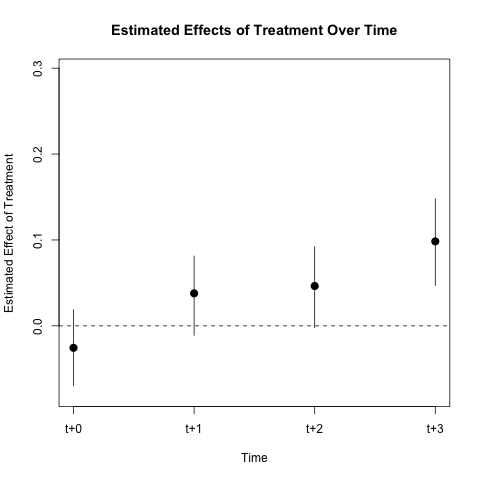
\includegraphics[width=0.75\textwidth]{Figures/panelmatch_logdefuncionespc.png}
       \captionsetup{justification=centering}
    
        
 \textbf{Note:} Figure \ref{fig:matching_violence} produced by propensity score matching that adjust for the treatment and covariate histories during the 5 year periods prior to the treatment. I report 95\% bootstrap confidence intervals clustered at the state level. Covariates include those used to generate Figure \ref{fig:event_study_agreements}. 
 
\end{figure}   
           
    
    
 \clearpage   
 
 %%%% NO ANTICIPATORY ASSUMPTION   
\section{Validating the no-anticipatory assumption \label{appendix:CDLZ}}

\renewcommand{\thetable}{C-\arabic{table}}
\setcounter{table}{0}
 \renewcommand{\thefigure}{C-\arabic{figure}}
\setcounter{figure}{0}
    
         
One way to address the no-anticipatory behavior is to assume that it can only occur in a fixed window prior to the electoral reform, say of one year, especially since the reform was announced in early 2013. However, for states that implemented reelection later this fixed window assumption would not suffice. In other words, only those early adopters of the reform would show unbiased estimates. Late adopters, however, would anticipate the term limit removal an act accordingly biasing the results upwardly.  
 
Another way to assess the no-anticipatory behavior from incumbents in this setting is test whether early vs late adopters differed in their estimated effects. Appendix Figure \ref{fig:CDLZ_agreements} presents \citet{cengiz_etal_2019} ``event-by-event analysis" that estimates treatment effects for each treated Mexican state (28 states) in the sample. States color differs if they are early (2015, red color) or late adopters (2016-2018, blue color). Specifically, I create state-event specific panel datasets and estimate state-specific estimates using separate regressions for each state. Each state dataset contains the treated state and all other states that never received treatment or received treatment after the sample window of $t+1$. For each state I estimate the following DiD regression: 
   
\begin{equation}
y_{mt}=\mu_m	 + \mu_t + \gamma Reform_{mt} + \epsilon_{mt}
\end{equation}

where $Reform_{mt}$ is an indicator variable that takes the value of 1 if the state implemented reelection. If there was evidence of strong incumbent anticipatory behavior, conditional on state covariates such as governor winning margin and alignment with Federal Executive, we would expect strong color clustering across similar estimated effects. In other words, if there is an endogenous response by states to implement the electoral reform, we would see that the positive (or negative) treatment effect would be only by those that implemented reelection earlier or later (events with the same color would be clustered). However, as seen in Appendix Figure \ref{fig:CDLZ_agreements}, this is not the case: there is wide variation in estimated coefficients across early (red) and late (blue) adopters of the reform, conditional and unconditional on state covariates. One would be concerned of the five blue states clustered in the positive end. However, if there was anticipation in these states they would only represent a downward bias of the main results found on the paper.  

\begin{figure}[h]
\centering
\caption{``Event-by-event analysis'' following \citet{cengiz_etal_2019}\\ -95\% confidence intervals-} 
\label{fig:CDLZ_agreements}
\includegraphics[width=0.5\textwidth]{Figures/CDLZ_cov_acuerdo.png}
       \captionsetup{justification=centering}
       \\
 {\textbf Note:} Estimate separate treatment effects for each event, i.e. each Mexican state in the sample. Each event dataset contains the treated state and all other states that never received treatment or received treatment after the sample window ($t+1$).   
\end{figure}     
   
For robustness, Appendix Figure \ref{fig:stacked_wcontrols_agreements} presents the ``stacked dataset analysis" from \citet{cengiz_etal_2019}. I take each of the ``event-by-event'' datasets from the Appendix Figure \ref{fig:CDLZ_agreements}, stack estimates by cohort and estimate one set of lead and lag variables not using prior treated units as controls. Appendix Figure \ref{fig:stacked_wcontrols_agreements} shows that conditional on state-level covariates, there is strong evidence of parallel trends as well as negative effect of reelection on delegation, but noisy.
       
    
\begin{figure}[H]
\centering
\caption{``Stacked dataset analysis'' following \citet{cengiz_etal_2019}\\ -95\% confidence intervals-} 
\label{fig:stacked_wcontrols_agreements}

\includegraphics[width=0.5\textwidth]{Figures/stacked_dataset_wcontrols_acuerdo.png}
       \captionsetup{justification=centering}
       \\
 {\textbf Note: Utilize estimated coefficients from Figure \ref{fig:CDLZ_agreements} and stack them in relative time, and estimate lead and lag variables to treatment following the event-by-event analysis setup, i.e. without treatment containment from using prior treated units of controls. Analysis done stacking at the cohort level, and adding municipality and year fixed effects, and clustered standard errors at the state level.}     
\end{figure}   




%
\chapter{Love the Candidate but Hate his Party: The Asymmetric Effects of Reelection Incentives on Partisan and Personal Incumbency Returns in Mexico}
\section{Introduction}

Over the past decades, an important theoretical and empirical literature has shown that incumbents may enjoy an electoral advantage \citep{ashworth_2012, cox_morgensten_1993, cox_katz_1996, ansolabehere_snyder_2000, ashworth_bdm_2008, ashworth_etal_2019} or suffer from an electoral disadvantage in the next election \citep{klasnja_2015, klasnja_titiunik_2017}. However, whether positive or negative, the electoral returns from incumbency mask the returns associated to parties and those exclusively of candidates. Disentangling both measures is important to understand citizens valuation of the electoral system and the existent electoral accountability \citep{mayhew_1974, fowler_hall_2014}. For instance, a partisan incumbency advantage might imply that voters believe parties control candidates behaviors, and thus would allow parties to hold a credible threat against renegade candidates. %The implications for a personal advantage are different, however: a personal advantage makes candidates vital for parties electoral success, leading the latter to allow more leeway to the former since retiring or switching parties may hurt parties electoral success. 
However, the implications of a personal incumbency advantage are different from the partisan one. A personal incumbency advantage makes retiring politicians support of new candidates vital for their electoral success, and stepping down or switching parties may hurt their parties in the next election. In this case, parties may allow more leeway to deviate from the party line to their members.\footnote{Likewise, a partisan incumbency disadvantage may imply citizens like partisan balance across time and may create incentives for candidates to differentiate themselves from their parties \citep{klasnja_titiunik_2017}. Contrastingly, a negative personal advantage may lead parties to differentiate themselves from candidates and stop their electoral support or remove the nomination in the next election.} Moreover, if a personal (partisan) effect exists and the partisan (personal) one is negligible it implies voters attribute actions in office to candidates (parties) and not their parties (candidates) or that a party (personal) dealignment might be taking place \citep{cox_katz_1996}.   
   
However, uncovering the partisan and personal incumbency advantage has proved methodologically challenging: every time a candidate is an incumbent so is its party so we cannot uncover the personal from the partisan incumbency advantages. This is true with the most widely used method to estimate the returns to incumbency, the regression discontinuity of close elections design (RDD), that conflates the personal and partisan incumbency advantage, even when the variables are defined in partisan terms (such as likelihood of the party winning or the party vote share) \citep{fowler_hall_2014}. To overcome these obstacles studies have tried to exploit cross-sectional comparisons between term limit and non-term limit races \citep{gelman_king_1990}, expiring and non-expiring careers \citep{fowler_hall_2014}, and changes in redistricting \citep{ansolabehere_snyder_2000, desposato_petrocik_2003, sekhon_titiunik_2012}. However, for identification they have relied on strong assumptions such as no differential pretrends in incumbency returns of term limit and non-term limit races \citep{fowler_hall_2014} or those that experience redistricting or not \citep{ansolabehere_snyder_2004}. %when comparing term-limit and non-term limit elections or expiring vs. non-expiring races  
Moreover,  while studies have used RDDs to rule out potential omitted variable bias coming from the correlation between current and future electoral success including parties reputation and candidates type \citep{klasnja_titiunik_2017}, recent evidence points that differences on the quality of incumbents and challengers -the so called scare-off effect- are still present \citep{eggers_2017}. 

This paper identifies the partisan and personal electoral returns to incumbency and solves the existent methodological difficulties faced by the literature. To do so, I use a difference-in-discontinuity of close elections design that exploits the 2014 Electoral Reform in Mexico that introduced reelection for mayors for the first time. The reform was staggered at the state level which allows us to compare the municipal elections in the not-yet-treated states where term limits exist to those in municipalities where incumbents have the possibility to reelect. Term limit incumbency returns identify the partisan effect as candidates cannot run again for office but their parties can. The incumbency advantage for elections with candidates up for reelection identifies both the personal and partisan advantages. By differentiating both measures -through the difference-in-discontinuity estimator- we are able to disentangle the personal from the partisan effect. The difference-in-difference setup allows us to test for parallel trends prior to treatment. Furthermore, by focusing on close elections we rule out potential omitted variables coming from differences in parties and electoral races. Additionally, this paper compares only incumbents in their first term which allows to rule out important endogenous concerns, particularly those arising from selection such as the difference in the ability or experience of incumbents \citep{ferraz_finan_2008, ferraz_finan_2011}.
 

Results show that the introduction of reelection generated an incumbency advantage, i.e., incumbents with the possibility to seek reelection hold an increasing likelihood to win office in the next election relative to municipalities where candidates are term limited. The same result is found by an increasing vote share in the next election as a measure for incumbency returns instead of the probability of winning office. However, this incumbency advantage masks an asymmetric effect. The incumbency advantage is a weighted average of a personal incumbency \emph{advantage} and a partisan incumbency \emph{disadvantage}. This implies incumbency became a personal affair when reelection was introduced in a country with a historically strong party-centered system, Mexico. Results also imply that if candidates retire or switch parties they will hurt the reelection chances of their parties. Not surprisingly, Mexico's 2014 Term Limit Reform introduced a ``party lock'' where mayors who wish to run for reelection cannot switch parties.  

To address  methodological concerns, we show that the results are not explained by pre-trends in incumbency advantage or heterogeneous treatment effects between different treated cohorts. Results are robust to various specifications, including varying the bandwidth for close elections and the functional form. Moreover no sorting into treatment or manipulation is found when running the typical McCrary test and testing for no discontinuous jump of other covariates at the winning margin threshold. 

The paper then explores the reasons behind the observed incumbency returns. I do not find evidence of a quality-based incumbency advantage as there are no differences in the quality of term limited and non-term limited incumbents for those who barely won and barely lost an election as measured by their education level. I do find evidence, however, of a resource based incumbency advantage where incumbents up for reelection who barely won an election to those with term limits and barely lost an election see an increase in the level of municipal revenues, and received an increase in federal and state fiscal transfers. A personal incumbency advantage may be explained by citizens expecting a higher budget or transfer in the future which they accrue directly to the effort of the incumbent rather than his party.

The main results of this paper coincide with those of \citet{fowler_hall_2014}, albeit for a different setting. They find that for the U.S. state legislatures the personal advantage is larger than found in previous literature, and that the partisan advantage is zero and possibly negative, as this paper does. This paper is the first one to compare party and personal advantage outside of the US. Moreover, while \citet{fowler_hall_2014} need to assume no pretrends prior to treatment for identification, the difference-in-discontinuity of close elections design allows us to test it and rule it out. 

This paper contributes to the literature on incumbency advantage in party-centered systems. A negative partisan incumbency return and positive personal one affects the way we think about parties-politicians relationships. Even in the case with strong party systems and a party-lock where candidates cannot run for reelection for other parties, parties cannot credibly threaten to withdraw their support from renegade members. In other words, the introduction of reelection debilitates parties power even in party-centered systems like Mexico generating candidate-centered electoral contests. This goes in line with the partisan dealignment literature, as the one seen in the electorate of the U.S in the post-war era  \citep{cox_katz_1996}, and shows the introduction of reelection to be a possible explanation of such separation between parties and representatives. It also introduced the possibility of new strategic politicians that may work to generate their own incumbency advantage  \citep{mayhew_1974, mckelvey_riezman_1992}.  
 
     
%Lastly, this work is closely related to the incumbency disadvantage literature, particularly the work of \citet{klasnja_titiunik_2017}. This paper studies a weak party system Brazil, and finds parties hold an incumbency disadvantage. They extend their results and show that Mexico and other term-limited countries hold a partisan incumbency disadvantage too. This paper finds the same partisan incumbency disadvantage for term limit races in Mexico, but shows that a personal incumbency advantage comes with the introduction of reelection incentives.

The next section delves into the importance of disentangling the personal from the partisan incumbency returns. I then describe the research design, followed by a brief overview of Mexico's 2014 Electoral Reform and data collection. Empirical results are then presented as well as a section with the mechanisms that explain the observed incumbency returns. %I close with a discussion on parties-members relationships when asymmetric personal and partisan incumbency returns are present. 


\section{Personal and Partisan Incumbency Advantage \label{sec:personal_vs_partisan}}

``Incumbency advantage is the additional electoral support a candidate gains due to his or her incumbent status'' (\citet{cox_morgensten_1993}, p. 329). It can be measured as either the difference in the vote share received by the incumbent in the election at $t+1$ from the vote share perceived at election $t$ or the difference in the likelihood of winning office. The literature has found several reasons behind an incumbency advantage from resources, visibility and power gained in office \citep{mayhew_1974, fiorina_1989, king_1991, cox_morgensten_1993}, to differences in the quality of incumbents and challengers \citep{cox_katz_1996, levitt_wolfram_1997, ansolabehere_snyder_2000, eggers_2017}, and the role of information on incumbent's ability and competence to voters \citep{ashworth_bdm_2008, ashworth_etal_2019}. On the other hand, incumbency disadvantage occurs if voters seek to balance power, they dislike parties, or prefer change  \citep{fowler_hall_2014, eggers_2017}, if candidates who replace incumbents or if challengers are of lower quality \citep{eggers_2017}, and/or if parties are weak to control candidates behavior and thus are punished by voters in the following election \citep{klasnja_titiunik_2017}.


Incumbency advantage can be decomposed into two components that allow for a better understanding on the relationship between voters, parties and their members: the partisan and the personal incumbency advantages. The partisan incumbency advantage is “the electoral benefit accruing to non-incumbent candidates by virtue of being from the incumbent party” (\citet{fowler_hall_2014}, p. 501). In other words, it speaks to the support parties win in the next election due to their incumbent status. The personal incumbency advantage, however, is a different concept: it is defined as the returns to incumbency that make a candidate better off as an incumbent relative to the counterfactual in which that candidate is not running as an incumbent but as a candidate for an open seat \citep{fowler_hall_2014}. As such, the personal incumbency advantage has been the typical measure of returns to incumbency in the literature. However, when incumbency returns are estimated the personal advantage is always conflated with the partisan advantage as parties and candidates are incumbents at the same time. 

Consider, for instance, the experiment described by \citet{lee_2008}. He states that in the case of US elections, ``[t]he ideal thought experiment for measuring the incumbency advantage would exogenously change the incumbent party in a district from, for example, Republican to Democrat, while keeping all other factors constant. The corresponding increase in Democrat electoral success in the next election would represent the overall electoral benefit due to being the incumbent party in the district" (p. 683). To proxy for this thought experiment, \citet{lee_2008} runs an RDD of close elections comparing the returns to incumbency in the next election $t+1$ for incumbents who barely win to those that barely lost at the election in $t$. However, the resulting incumbency returns provide an entangled average effect of both the personal and partisan incumbency return. Moreover, experiments such as this tend to interpret the results as accruing solely to incumbents rather than their parties, and do not consider voters may value differentially parties and their representatives. 

Substantively, these two concepts provide different interpretations of the electoral system. Overall there are six possibilities. First, we can observe a  partisan and personal incumbency \emph{advantage}. In this case, positive incumbency returns increase the concern that incumbents may insulate themselves from electoral threats, and debilitate their accountability to constituents \citep{ashworth_etal_2019, cox_katz_2002}. Parties might not have incentives to monitor or exercise control over their members given their electoral isolation as well as the potential negative consequences of standing against incumbents with high personal electoral returns from office. Overall, a personal and partisan incumbency advantage may signal that voters accrue actions of candidates to both parties and representatives, and may lead parties and candidates to isolate from the electoral connection created by reelection \citep{mayhew_1974}. 

 In a second scenario, we can observe both a partisan and personal incumbency \emph{disadvantages}. In developing countries with term limits such as Brazil, Mexico and Colombia, \citet{klasnja_titiunik_2017} find strong evidence of an incumbency disadvantage. A negative partisan incumbency may show constituents prefer partisan balance \citep{folke_snyder_2012}, believe the ``grass-is-greener'' with other parties \citep{bhatia_turan_2013}, dislike parties but not their members \citep{parker_davidson_1979}, or have suffered from institutional changes such as redistricting that decreases electoral support of incumbents \citep{ansolabehere_snyder_2000, desposato_petrocik_2003}, for example. A negative personal incumbency might signal voters see incumbent politicians as too corrupt and prefer new candidates to hold office in the next turn. In this setting, parties choice might be to nominate new candidates to contend for office despite incumbents holding the possibility to reelect. Incumbents up for reelection may choose to switch parties or run for other political positions at the state or federal level in which case they may be very diligent in following the party line. 
  
 Third, we can observe an asymmetry where a personal incumbency \emph{advantage} might coincide with a partisan incumbency \emph{disadvantage}. Parties no longer hold a credible threat to punish renegade incumbents. Moreover, a retirement slump might lead parties to lose votes when the incumbent retires \citep{alford_brady_1989} or in the presence of term limits \citep{ansolabehere_snyder_2004}. Candidates may also hold incentives to differentiate themselves from their parties through various personalistic strategies as voters may attribute the actions of candidates only to them and not their parties. A positive personal incumbency might also imply voters transfer their support to whomever the current incumbent wishes to endorse if they are retiring. A personal incumbency advantage might also signal a sophomore surge when a new representative will garner more votes when running for his first reelection than when she was a challenger \citep{erikson_1971, alford_brady_1989}. 
  
 
 Fourth, an asymmetry with a personal incumbency \emph{disadvantage} might coexist with a partisan incumbency \emph{advantage}. In this case, citizens might see representatives as lame ducks in office and attribute their actions to their parties. In this setting we may also have that retiring incumbents are not invited to support new candidates from their party as this may damage their electoral success in the coming election. More importantly, this scenario makes elections party-centered rather than candidate-centered, with parties holding a credible threat to withdraw their support or nomination for dissident members since new candidates will benefit from the positive partisan electoral return for the next election.  

The two additional scenarios are for either partisan or personal incumbency returns to be negligible. When the personal incumbency is not different from zero, it may imply that actions of incumbents do not affect the parties return from incumbency if they choose to step aside by switching parties or retiring. On the contrary, a negligible partisan incumbency return makes the branding and attributes of parties not as important for voters even if they rely on partisan labels to define their vote. Moreover, voters in this setting might see the actions of incumbents as separate from their parties \citep{fowler_hall_2014}. 

A negligible or negative partisan incumbency return and a personal incumbency advantage is strongly tied to the large literature on partisan dealignment. As \citet{beck_1985} notes, an electorate that appears to be highly partisan may be just a facade if ``partisanship is merely an expression of momentary vote choice'' (p. 233). This dealignment trend has been identified in the US since 1953 due to generational changes, as well as the weakening of group bases of party support and increase electoral competition \citep{beck_1977, norpoth_rusk_1982}, in Britain since 1970 due to retrospective voting \citep{alt_1977}, the Netherlands since the late 1960s due to vote switching and the decline in political cohesion of groups \citep{irwin_dittrich} and Denmark, Norway and Sweden were class voting declined since the 1970s \citep{borre_1995}. In Mexico -the study case at hand in this paper-, winning margins have substantively declined since the move to democracy in 2000, while party bases have constantly migrated from one party to another, and from one political leader to another. Besides the case of the US, however, partisanship has been linked too closely to candidate vote choice to assess whether dealignment ocurrs.  However, the existence of a strong personal incumbency advantage relative to a negligible or negative partisan one, for example, may portray a dealignment of citizens from mass politics and into more personalistic electoral contests. 
   
In summary, evaluating an electoral system requires the identification of the personal and partisan incumbency returns. Limiting to the former provides and incomplete picture of the relationship between voters, parties and their members. The next section describes methodological problems behind the literature estimation of the incumbency advantage and describes the research design used in this paper to disentangle the personal from the partisan incumbency advantages. 


%Appendix \ref{appendix:rdd} runs a similar experiment with an RDD with close elections and optimal bandwidths following \citet{calonicoetal_2014} but considering all mayoral races from 1989 to 2018. Since this time period covers races before and after the 2014 Electoral Reform, i.e., with and without term limits, I ran two separate RDDs. I find an incumbency disadvantage of -11\% significant to the 1\% level, using both a linear and quadratic polynomial. An incumbency disadvantage is also found using vote share of -4\% significant to the 1\% level using a linear and quadratic polynomial as well. Contrastingly, for elections that removed term limits and introduced reelection for mayors we observe a positive but not significant effect on incumbency returns, using both the probability of victory or the winning margin in the next election. In other words, it seems reelection erased the negative returns to parties in Mexico. However, these incumbency returns estimates do not allow us to assess whether incumbency became a personal matter when reelection was introduced or remained mainly a partisan one. In other words, we are unable to securely state that Mexico moved from a party to a candidate centered system due to the introduction of reelection and the strengthening of voter accountability, and what this implies in terms of of voters, parties, and representatives dynamics.

 %Moreover, these estimates may be biased in three ways. First, by comparing term limit and non-term limit elections we need to assume there are parallel trends which might not be the case and an RDD does not allow us to test this assumption. Second, there might exist heterogeneous treatment effects across different treatment cohorts since the 2014 Electoral Reform was implemented in a staggered way at the state level. Lastly, as \citet{eggers_2017} notes even when comparing close elections in a regression discontinuity design, a potential difference in the quality of incumbents and challengers may still exist. The next section addresses these methodological issues by describing the research design used in the paper.  


  
\section{Research Design to Disentangle the Personal from the Partisan Incumbency Advantage \label{sec:design}}

\subsection{Research Designs Explored in the Literature \label{sec:design_literature}}
The typical methodological tool to study incumbency returns is the regression discontinuity of close elections design (RDD) \citep{thistlethwaite_etal_1960, imbens_lemieux_2008, lee_2008}. Since election results are not exogenous, we move to a local environment where we compare very close elections. Presumably, by comparing incumbents that barely won to those that barely lost we we keep constant municipal characteristics on each side of the cutoff \citep{lee_2008, boas_hidalgo_2011, broockman_2009, butler_2009, dalbo_etal_2009, querubin_snyder_2013, titiunik_2012, klasnja_titiunik_2017}. However, recent evidence shows that even with RDDs of close elections barely winners and losers might differ in terms of quality \citep{eggers_2017, caughey_sekhon_2011, grimmer_etal_2012}. Problems include incumbents being better than challengers or a potential scare-off effect. 
   
RDDs, moreover, cannot disentangle the personal and party incumbency advantages. As \citet{erikson_titiunik_2015} show, the RDD incumbency advantage coefficient is defined as 2*Partisan Advantage + 2*Pr(Winner Runs Again)*Personal Advantage. The partisan incumbency advantage is doubled because ``winning party has both the benefit of being the incumbent party and the benefit of the other party not having this advantage'' (\citet{fowler_hall_2014}, p. 512). For the same reason, the personal incumbency advantage is multiplied by two, as well as the probability that the winner of the first election runs for re-election since this is not always the case. This makes the partisan and personal advantage unidentified when we estimate the RDD coefficient.

One possibility to disentangle the partisan from the personal incumbency disadvantages is to compare two different regression discontinuity models as done by \citet{fowler_hall_2014}. The first RDD compares the probability of winning in the election at $t+1$ for parties that barely won to those that barely lost in the election at $t$, all which are term limited. Since candidates cannot remain in office more than the appointed term but their parties can participate in the next election, this RDD yields the partisan incumbency advantage. The second RDD compares the probability of wining in the election at $t+1$ for politicians that can seek reelection and barely won in the election in $t$ to those up for reelection and barely lost in $t$. In this case, the RDD coefficient shows the partisan and the personal incumbency advantages. Thus, the difference between both RDD models yields the personal incumbency advantage. For this difference to yield identified personal and partisan effects, we need to rely on three identification assumptions. First, potential outcomes are continuous at the forcing variable threshold, i.e. the electoral margin vote share usually normalized at zero. The second assumption states that the average personal and partisan incumbency advantages in a given election do not vary differently across time for those with and without term limits. This assumption is the typical parallel trend assumption in difference-in-difference (DiD) designs. As with DiDs, the parallel trend assumption does not imply that term limit and non-term limit elections are the same across covariates, but that the vary similarly across time prior to treatment. However, in the case of term limit and non-term limit races it is a very strong assumption. The third identification assumption is that there is no change in the quality of incumbents when an incumbent retires as is replaced by a new candidate. 

Other papers have tried to disentangle the personal from the partisan incumbency advantage. By definition, a personal incumbency advantage comes from comparing the electoral returns of an incumbent up for reelection to the counterfactual in which the incumbent had run for the same race, at the same time, in the same locality, but not as an incumbent. A similar experiment in mind is that of \citet{gelman_king_1990} that compares two scenarios, one where the incumbent legislator runs, and another when an incumbent legislator retires, and both belong to the same party. Holding the party constant allows to tease the party incumbency advantage. The concern is that races where incumbents retire might not have the same trends to those where they do not. Another experiment has exploited redistricting, where the personal incumbency return comes from comparing  new voters who are first experiencing and incumbent are compared to old voters who already know the incumbent \citep{sekhon_titiunik_2012}. The problem, however, is that even conditional on covariates old and new voters may differ introducing potential bias as noted by a large gerrymandering literature. 

\subsection{Research Design}

To overcome the empirical challenges faced by the literature and relax the assumptions to identify the personal and partisan incumbency advantages, I use a difference-in-discontinuity of close elections design that exploits the staggered rollout of an Electoral Reform in Mexico in 2014 that introduced reelection for up to 2 terms for mayors. Let me describe the two embedded models that make up the research design, a regression discontinuity of close elections design and a difference-in-difference design. 

First, in a regression discontinuity design all units have a score, and those units above a cutoff receive the treatment while those below do not. Under assumptions such as no sorting into treatment, a comparison of the observations below and above the cutoff define a local space in which we can estimate the causal effects of the treatment on a given outcome. In this paper, the unit of observation is the municipality $m$, and the municipality is treated if the incumbent's margin of victory (the score) -defined as the incumbent's vote share minus the vote share of the runner up- is above the cutoff, and not treated if its below. The cutoff that determines the electoral victory is normalized to zero: the incumbent wins the election when its vote margin is positive and loses otherwise. In Mexico, the number of political parties that wins a mayoral election is large. For parsimony, this paper presents results for the incumbent party, whichever party this may be. The incumbent party analysis following \citet{klasnja_titiunik_2017} identifies the party that wins the election at $t+1$ and studies the effects of this party's barely winning or losing at $t$ on outcomes at election $t+1$. Given this setup, we require at least three rounds of elections. 

If municipalities where an incumbent barely wins the election at $t$ (the treatment group) are not different from the municipalities where an incumbent barely loses the election at $t$ (the control group), the RD coefficient yields the average effect at the cutoff of a party winning office at $t$ on the electoral success at the election at $t+1$, i.e. the incumbency advantage. Certain assumptions need to hold though, specially no sorting into treatment, and that potential outcomes are continuous at the forcing variable threshold (when the margin of victory=0). This incumbency advantage, however, conflates the partisan from the personal incumbency advantages as described in the last section. How then can we disentangle both estimates? For this we rely on an additional model, a difference-in-difference design that leverages the introduction of the 2014 Electoral Reform in Mexico.

The Electoral Reform creates two experimental groups. First, not-yet-treated municipalities are those with term limits whose mayors are forced to retire but not their parties who can run for office. By comparing incumbents that barely won to those that barely lost in the election at $t$, term limit municipalities identify the partisan incumbency advantage (A). Treated municipalities, however, have incumbents that can run up for reelection as well as their current parties since they cannot switch parties given the party-lock of the reform. By comparing incumbents up for reelection that barely won to those that barely lost in the election at $t$, non-term limit municipalities identify both the partisan (A) and personal (B) incumbency advantages (i.e., A+B). By estimating the difference between term limit and non-term limit municipalities, on either side of the winning margin threshold we obtain an unbiased estimate of the personal incumbency advantage (A+B-A=B). This estimate is what we called the difference-in-discontinuity of close elections estimator. In this model, instead of needing to assume for term-limit and non-term limit municipalities not to vary differently across time, we can test for parallel trends. 

Lastly, the difference-in-discontinuity design in this paper only compares first term mayors in term limit and non-term limit races. A first term mayor that can reelect and a first term mayor who is term-limited have won an election once, and thus have the same selection pressures but different electoral incentives. The difference between them yields the election incentive effect. There are no selection effects, however. To estimate them we would have to compare either a term-limited mayor who was won election once to a term-limited mayor who has won election twice, where both are facing the same election incentives but hold different selection histories. The same could be done by comparing first term mayor that can reelection and has won election once to a mayor that can reelect and has won election twice. This experiment to isolate the election from the selection effect is done by \citet{ashworth_2012}. Thus, the difference-in-discontinuity estimator for first term mayors erases selection concerns, including differences of experience or ability \citep{ferraz_finan_2008, ferraz_finan_2011}. 

%For clarity on the treatment, the next subsection provides a description of the 2014 Term Limit Reform in Mexico.  

\subsection{Mexico's 2014 Term Limit Reform}

In Mexico in 1933, the Partido Nacional Revolucionario (PNR, the former PRI) imposed a ban on reelection making all presidential, gubernatorial, legislative and mayoral elections term limited. The motivations behind this constitutional amendment was to control self-motivated politicians to deviate from the party line in any of the multi-level party structure. The famous phrase in Mexican politics ``if you move you don't appear in the photo'' (\emph{si te mueves no apareces en la foto}) which implies that if you deviate from the party line you will be left aside, shows the spirit of the PNR and later the PRI to weaken  local party bosses and allow the party to control political careers at the federal, state and local level by limiting reelection \citep{weldon_2003}. 

Eighty years later in 2013, the new Peña Nieto administration pushed an aggressive set of reforms to privatize the energy sector and modify the existent fiscal institutions in the country. To increase the probability of success, the PRI with the PAN and PRD, the three main political parties at the time, lead the construction of the Mexican Pact Accord, a series of roundtables intended to negotiate the energy sector reform along a set of structural reforms that had failed to pass through congress due to political gridlocks. By the end of May 2013, a roundtable to discuss an electoral reform was installed. Specifically, commitment 94 of the Pact Accord introduced reelection for discussion. While the Electoral Reform was not under PRI's set of desired reforms, the opposition utilize it as a bargaining chip to approve those pursued by the PRI \citep{zamitiz_2017}. However, due to lack of consensus, the Mexican Pact Accord did not submit an electoral reform proposal to Congress and left the bargaining process to the Senate. Two months later, on July 24, 2013, PAN and PRD pushed a political-electoral reform with 36 law changes that included  the creation of a National Electoral Institute (INE for its acronym in Spanish) that would be in charge of federal, state and local elections, and reelection for federal and local legislators, as well as mayors. Given state-level opposition to the reform, Senate leaders from the PAN and PRD chose to approve the electoral reform in December 2, 2013, before the energy reform, and thus increased their political leverage over the PRI. By January 2014, PAN and PRD threatened to not support the energy reform  if the PRI did not push local state legislatures from approving the electoral reform which at the time where blocking the reform given pressure from various PRI governors.\footnote{The Mexican Constitution establishes that the majority of state legislatures need to approve constitutional reforms for reforms to be valid.} The political gridlock led former President Peña Nieto to ``exhort" local legislators to approve the electoral reform. On January 31, 2014, the reform was promulgated by the President and contained three main changes: (1) the creation of the INE; (2) removal of term limits of mayors for up to 2 terms;\footnote{The reform also introduced reelection for local and federal legislators who are allowed to reelected up to 4 consecutive terms.} and (3) the introduction of a ``party-lock"	where mayors or legislators who wish to get reelected could not switch parties.\footnote{For more details on the political background of the 2014 Electoral Reform please see Appendix A in \citet{ch_2021}.}

The reform granted discretion to state legislatures to define the number of terms mayors could reelect as well as the reelection implementation date. All states approved up to 2 consecutive reelection terms for mayors except for the states of Nayarit, Hidalgo, Tlaxcala and Veracruz who did not allow consecutive reelection. 

\begin{figure}[H]   
\centering 
\caption{Mexican States Electoral Reform Treatment Status}
\label{fig:treatment_status}
\includegraphics[width=0.75\textwidth]{Chapter2/Figures_incumbency/reform_treatmentstatus.pdf}     
\captionsetup{justification=centering} 
\end{figure}     
  
  
In regards to the implementation date, the Electoral Reform established that it would not affect any of the 2014 elections. Figure \ref{fig:treatment_status} describes the implementation period or treatment status of each of Mexico's 32 states.\footnote{Mexican states share the same administrative level as US states.} This figures allows to visualize the staggered rollout of the term limit removal. We have five timing groups: (1) 15 states who implemented reelection in 2015; (2) 9 who implemented reelection in 2016; (3) Coahuila who implemented reelection in 2017; (4) 4 states that implemented reelection in 2018; and (5) 4 states that will never be treated since they bypassed the reform by not allowing consecutive reelection (Hidalgo, Nayarit, Tlaxcala and Veracruz). Treatment in Figure \ref{fig:treatment_status} implies the following: Campeche, for example, begin treated starting in 2015 means that mayors elected in 2015 can run for reelection in the next election of 2018, as well as that of 2021 if they won in the previous one. Similarly, mayors in Chihuahua elected in 2016 can run for reelection in 2019, as well as 2022 since the reform allows mayors to reelect up to two consecutive terms. 

Evidence suggests that the differences in timing is a function of the staggered calendar of gubernatorial elections. As noted by \citet{motolinia_2020}, at the moment the reform was approved some governors were starting their terms while others were ending them. Those ending their terms had greater incentives to introduce reelection early on given that they could still apply political influence after leaving office by choosing people of their liking. In other words, governors influence in candidate selection of mayors seems to explain most of the variation in the staggered calendar of the implementation of the reform. For causal identification, it is important in empirical specifications to control for governors political power. 

\subsection{Empirical Specification} 
  
I estimate  a difference-in-discontinuity in close elections model that exploits the 2014 Electoral Reform that removed term limits for mayors in Mexico. To do so, I follow \citet{grembi_etal_2017} to estimate the boundary points of four regression functions of the probability of winning office (or the vote share) in the next election at $t+1$ ($Y_{m,t+1}$) on the winning margin of the election at $t$ for municipality $m$ and normalized at zero ($Margin_{m,t}$): two regressions on either side of the winning margin threshold (i.e., when $Margin_{m,t}$=0), before and after the implementation of the Term Limit Reform at $t_0$. Following \citet{gelman_imbens2014}, I fit a local linear regression for the observations distributed within an  \citet{calonicoetal_2014} optimal bandwidth distance $h$ to the forcing variable cutoff, for either side of $Margin_{m,t}$ before and after the implemenation of the Reform at $t_0$.\footnote{A rectangular kernel would give the same results as taking $E[Y]$ at a given bin on the distance to the cutting threshold. Other types of kernels, such as a triangular kernel, gives more weight to observations closer to the cutoff. I choose the latter for all estimations presented while estimations using a rectangular kernel are available upon request. Results are almost unchanged using the latter rather than the former.} In other words, I compare only municipalities in close elections and thus restrict the sample to those within a certain distance $h$ to the threshold, i.e. $Margin_{m,t} \in [Margin_{b-h}, Margin_{b+h}]$.  

The specification of the difference-in-discontinuity in close elections design is the following:

\begin{equation}
\small
\label{eq:abraham}
\begin{split}
Y_{m,t+1}=\mu_m + \lambda_t + \delta_1 f_{(.)}(VoteShareMargin)_{m,t} \\  
+ Win_{m,t}(\gamma_0 + \gamma_1 f_{(.)}(VoteShareMargin)_{m,t}) \\ + Reform_{m,t}[\alpha_o + \alpha_1f_{(.)}(VoteShareMargin)_{m,t} 
+ Win_{m,t}(\beta_0 + \beta_1 f_{(.)}(VoteShareMargin)_{m,t} )] \\ + \mathbf{X}_{s(m),t} \Phi + \epsilon_{m,t}
\end{split}
\end{equation}   

where $Y_{m,t+1}$ is either (a) a dummy=1 if party wins the following election at $t+1$, =0 otherwise, or (b) the vote share in election at $t+1$, 0 otherwise. $Win_{m,t}$ is a dummy=1 if an incumbent from $t-1$ barely lost the election at $t$, =0 if he lost. $Reform_{m,t}$ is a dummy=1 if a municipality implemented reelection for mayors, =0 otherwise, i.e. a post-treatment indicator. $f_{(.)}(VoteShareMargin)_{m,t}$ is the RD polynomial on winning margin for municipal election $m$ at calendar time $t$, having $f_{(.)}$ an \emph{n}th order polynomial of the forcing variable $VoteShareMargin_{m,t}$, which in this paper will be only a linear and quadratic polynomials.\footnote{Equation \ref{eq:abraham} shows the specification for the linear case. For the quadratic case, we would expand the equation to include all linear and quadratic polynomials interactions to have a fully saturated model.} $\mu_m$ and $\lambda_t$ are municipality and year fixed effects, with $\mathbf{X}_{s(m),t}$ a battery of controls including a dummy on the party alignment of the mayor with the governor, and the winning margin of the governor to proxy for governors influence in local politics. Standard errors are clustered at the state level as that is the level of treatment of the Electoral Reform in Mexico. 

The coefficient $\gamma_0$ is the regression discontinuity estimator that measures the incumbency returns for term-limited mayors. In other words, $\gamma_0$ captures the partisan incumbency advantage as term limited incumbents cannot run again for office but their parties can. The coefficient $\alpha_0$ is the difference-in-difference estimator on the effect of the Term Limit Reform on the probability of winning in the election at $t+1$. Conditional on municipal and period fixed effects, as well as other covariates, this estimator represents the difference in the probability of winning (or the vote share) in the next election $t+1$ for mayors without term limits to those with term limits. This coefficient does not measure an incumbency advantage. Lastly, the coefficient $\beta_0$ is the difference-in-discontinuity estimator that identifies the personal incumbency advantage by comparing municipalities where an incumbent barely wins an election to municipalities where an incumbent barely loses ($Win_{m,t}$), before and after term limit removal ($Reform_{m,t}$), i.e. the treatment $PersonalIncumbency_{m,t}=Reform_{m,t} \cdot Win_{m,t}$. Importantly, $\gamma_0$ and $\beta_0$ are divided by 2*Pr(Incumbent Runs Again) as some incumbents may retire in election $t$ as described in Section \ref{sec:design_literature}. 
 

\subsection{Data}  

The two main outcomes of interest are (i) an indicator of whether the incumbent party wins the mayoral office in election at $t+1$, and (ii) the vote share of the incumbent party in election at $t+1$. As described in the last section since the number of parties that compete for Mexican mayoral elections and win is large, I restrict the analysis only to incumbent parties following \citet{klasnja_titiunik_2017}. To do so, we need to identify a party that wins the election at $t-1$ and study the effects of this incumbent winning or losing at $t$ on the electoral outcomes (i) and (ii) at election $t+1$. For this we need at least three elections per municipality. The data covers all election years from 2006 to 2018. This allows to have at least two pre-reform election per municipality. 

For example, for the state of Michoacan we consider data for the elections of 2012 ($t-1$), 2015 ($t$) when the Electoral Reform was implemented, and 2018 ($t+1$). To check for pre-reform parallel trends we need additional elections prior to 2012. I include at least two full three-election cycles prior to treatment. Lets use the example of Michoacan again: the first cycle considers the election 2006 ($t-1$) to define the party that is the incumbent, who barely looses or wins at election at 2009 ($t$) on the electoral outcomes at the election at 2012 ($t+1$); the second cycle considers the election 2009 ($t-1$) to define the party that is the incumbent, who barely looses or wins at election at 2012 ($t$) on the electoral outcomes at the election at 2015 ($t+1$). To test for parallel trends we will only observe two coefficients prior to treatment of the incumbency advantage for the state of Michoacan: 2009 (as $t$ for the first cycle) on its effect on electoral outcomes at 2012 (as $t+1$ for the first cycle), and 2012 (as $t$ for the second cycle) on its effect on electoral outcomes at 2015 (as $t+1$ for the second cycle).   For other states these years may vary since each state holds different electoral calendars.\footnote{Municipal electoral calendars vary by state. However, almost all municipalities have three year terms with the exception of some municipalities with non-aligned electoral calendars with State-level ones, or other political circumstances.}

%However, since we generally have a reference period in event-study models, we do not show incumbency advantage results for the second cycle of 2012 (as $t$) and 2015 (as $t+1$).

To measure incumbent quality, I web-scraped professional titles and other characteristics for all municipal mayors in Mexico from 2010 to 2019 from the National Information Municipal System (SNIM for its abbreviation in Spanish). This novel database allows me to test for quality-based incumbency advantages.

I use several measures to proxy for the resources and effort placed by incumbents once in office. I use the National Institute of Statistics and Geography (INEGI for its acronym in Spanish) municipal level data on revenues and expenses from 2010 to 2018. I use data on total municipal revenues, as well as its subcomponents, specifically those coming from taxes, including property and estate taxes, as well as those from production, consumption and transaction taxes. These variables were deflated and are expressed in million pesos.\footnote{One dollar = 20 Mexican pesos approximately.} This data is further described in Section \ref{sec:mechanisms} while Appendix Table \ref{tab:descriptive} presents descriptive statistics.
  
\section{Main Results \label{sec:results}}

Table \ref{tab:naive_twfe} shows the $\gamma_0$ or coefficient of the partisan incumbency advantage, $\alpha_0$ or the coefficient of the difference in the probability of wining in the next election between term and non-term limited incumbents, and $\beta_0$ or the personal incumbency advantage. First, we observe that the introduction of reelection generated an incumbency \emph{advantage}, i.e. $\gamma_0 + \beta_0$ is equal to 4.5\% but not significant when using the probability of winning in the next election as outcome, and 4.6\% significant to the 1\% level for the linear specification. Results are similar for the quadratic polynomial specification. However, this positive incumbency advantage masks an asymmetry. First, we find a partisan incumbency \emph{disadvantage} of -5.38\% (not significant) in the probability of winning office in the next election, and a -3.32\% significant to the 1\% in the vote share in the next election [for the linear case and results are similar for the quadratic one]. These results are smaller than the ones identified in other Latin American cases like Brazil (-7.5\%), Colombia (-10\%) and Peru (-8.5\%) by \citet{klasnja_titiunik_2017}.\footnote{These numbers are the coefficients presented by \citet{klasnja_titiunik_2017} but divided by 2 and adjusted for the probability of running for office, a correction not done for these estimates.} 
 
\begin{table}[h]\def\sym#1{\ifmmode^{#1}\else\(^{#1}\)\fi}
\centering
\caption{Partisan and Personal Incumbency Advantage, Difference-in-Discontinuity of Close Elections Model}
\label{tab:naive_twfe}
\scalebox{0.75}{ 

\begin{tabular}{l*{4}{c}}
\hline \hline 
   
              &\multicolumn{2}{c}{\begin{tabular}[c]{@{}l@{}} Probability of winning, \\ Election at t+1\end{tabular}}&\multicolumn{2}{c}{\begin{tabular}[c]{@{}l@{}}  Vote Share,  \\ Election at t+1 \end{tabular}}\\\cmidrule(lr){2-3}\cmidrule(lr){4-5}
            &\multicolumn{1}{c}{(1)}         &\multicolumn{1}{c}{(2)}         &\multicolumn{1}{c}{(3)}         &\multicolumn{1}{c}{(4)}         \\
\addlinespace
Term Limit Reform ($\alpha\_0$)&      0.1780\sym{**} &      0.1789\sym{**} &      0.1656\sym{**} &      0.1656\sym{**} \\
            &    (0.0770)         &    (0.0770)         &    (0.0773)         &    (0.0771)         \\
\addlinespace
\begin{tabular}[c]{@{}l@{}} Dummy win, Election at t ($\gamma\_0$) \\ (Partisan Incumbency Advantage)\end{tabular}&     -0.0538         &     -0.0537         &     -0.0332\sym{***}&     -0.0332\sym{***}\\
            &    (0.0389)         &    (0.0392)         &    (0.0111)         &    (0.0110)         \\
\addlinespace
\begin{tabular}[c]{@{}l@{}} Interaction: Reform X Win Election at t ($\beta\_0$)  \\ (Personal Incumbency Advantage)\end{tabular}&      0.0986\sym{*}  &      0.0979         &      0.0788\sym{***}&      0.0787\sym{***}\\
            &    (0.0580)         &    (0.0591)         &    (0.0208)         &    (0.0209)         \\
\addlinespace
Observations&        2247         &        2247         &        1892         &        1892         \\
R-squared   &       0.535         &       0.535         &       0.558         &       0.558         \\
Municipal FE&  \checkmark         &  \checkmark         &  \checkmark         &  \checkmark         \\
Year FE     &  \checkmark         &  \checkmark         &  \checkmark         &  \checkmark         \\
Controls$^a$&                     &                     &                     &                     \\
Polynomial  &      linear         &   quadratic         &      linear         &   quadratic         \\
Incumbency Advantage: Partisan ($\gamma\_0$) + Personal($\beta\_0$)&  $0.045^{}$         &  $0.044^{}$         &$0.046^{***}$         &$0.045^{***}$         \\
SE(Incumbency Advantage)&       0.036         &       0.036         &       0.017         &       0.017         \\
Difference:Personal($\beta\_0$)-Partisan($\gamma\_0$)& $0.1523^{}$         & $0.1516^{}$         &$0.1119^{***}$         &$0.1119^{***}$         \\
SE(Difference)&      0.0919         &      0.0935         &      0.0289         &      0.0290         \\
   
     
      
\hline \hline 
\multicolumn{5}{p{1.2\textwidth}}{\footnotesize{Notes: Standard errors in parentheses are clustered at the state level. Significance-level: $^{***}$ 1\%; $^{**}$ 5\%; and $^*$ 10\%, that refer to two-sided t-test.$^a$ Pretreatment controls include: governor winning margin; party alignment with the President;  party alignment with the Governor; and logged population.}} \\
\end{tabular}
}
\end{table}    


Second, we observe a personal incumbency \emph{advantage} of 9.86\% significant to the 10\% in the probability of winning office, and of 7.88\% significant to the 1\% level for vote share in the next election [for the linear case and results are similar for the quadratic one]. The personal incumbency advantage found is not small representing almost half a standard deviation for the vote share, and a quarter of a standard deviation for the probability of winning office in the next election. Interestingly, the personal incumbency advantage is similar to the one find by \citet{fowler_hall_2014} for the case of the US of 8.8\%. They also find a negative partisan incumbency of -2\% but not significant.  

Table \ref{tab:naive_twfe} shows that prior to the introduction of the Electoral Reform Mexico's mayoral elections showed an incumbency disadvantage (a partisan one since their where term limits). This result has been confirmed by \citet{klasnja_titiunik_2017} who run a regression discontinuity design for close elections considering all elections from 1997 to 2009 in Mexico. However, once reelection is introduced a decrease in the incumbency disadvantage is observed and as noted in Table \ref{tab:naive_twfe} it even became positive and not different from zero. This decay in the incumbency disadvantage with the removal of term limits is similar to the finding by \citet{klasnja_titiunik_2017} when comparing the incumbency returns from countries with term limits -mainly Brazil, Mexico, and Colombia-  to those with indefinite reelection -Peru, Chile and Costa Rica: while the former show an average incumbency disadvantage of -19\% (significant to the 1\% level) in the probability of winning office the latter show an incumbency disadvantage of -2\% (non-significant). In the case of \citet{klasnja_titiunik_2017} they believe incumbency disadvantage is explained by voters blaming weak parties from not being able to sanction their members from undesirable behavior in office, specially when they are term limited and there is no need to be responsive for voters. They mention that the removal of term limits could have strengthen the accountability between voters and representatives which should decrease the responsibility put on parties to control their members decreasing the incumbency disadvantage. The asymmetry found in Table \ref{tab:naive_twfe} offers a closely related logic: reelection creates an ``electoral connection'' between voters and incumbents \citep{mayhew_1974}; as a result, a personal incumbency advantage is created signaling that voters believe incumbents and not their parties are responsible for policy actions. In other words, a personal incumbency advantage is the main driver in the decrease in incumbency disadvantage in Mexico, and plausibly other countries too. Moreover, this result speaks to a potential party dealignment in Mexican politics after the introduction of reelection. Not only has the country experienced a decrease in winning margins and various changes in party bases in the last two decades, but citizens at the municipal level are associating policy actions to representatives rather than their parties.   


Lastly, it is important to notice that mayors up for reelection had a higher probability of winning office in the next election relative to term-limited mayors whose parties will run again. This is not a measure of incumbency advantage but just a difference in the probability of winning office. The probability is not small, however, it represents a greater likelihood of 17.8\% significant to the 5\% level of winning office in the next election, and a greater vote share of 16.6\% in the next election. 
   
\subsection{Identification assumptions} 

To validate causal effects three identification assumptions need to hold. First, parallel trends for both incumbency advantage measures need to hold. As seen in Figure \ref{fig:event_study_personal}  this is the case for both the probability of winning and vote share at election $t+1$. This Figure shows an event study design of the same data used to estimate Table \ref{tab:naive_twfe} but constructing $t$ year indicators relative to treatment implementation. The period $t=0$ represents the year in which the Electoral Reform was implemented. Periods prior to $t=0$ speak to the years prior to the implementation of the reform. For example, $t-6$ represents two election cycles prior to $t=0$ since for some municipalities electoral cycles last 3 years.  $t-5$ and $t-4$ also represent two election cycles prior to the implementation of the reform at $t$ but for municipalities where their calendars gave only 2 or 1 years for mayors in office, which corresponds to states that where aligning their municipal and gubernatorial calendars (E.g., Puebla). Figure \ref{fig:event_study_personal} omits the election prior to the implementation of the Reform to serve as comparison group: these is the period three years prior to $t=0$, i.e. $t-3$. There were no elections in years $t-2$ and $t-1$. Thus, estimated coefficients are interpreted as the difference relative to the election prior to the implementation of the Reform.\footnote{Potential treatment effect heterogeneity of the different treatment cohorts of the Reform may introduce bias to the difference-in-discontinuity estimators. I follow \citet{abraham_sun_2020} and run a cohort weighted event study design that takes into account treatment effect heterogeneity. Results show parallel trends and similar results to those of  Figure \ref{fig:event_study_personal}. Results available upon request.} Figure \ref{fig:event_study_personal} shows the difference-in-discontinuity estimator $\beta_0$, i.e. the personal incumbency advantage before and after the implementation of the Reform. Parallel trends are found for both the linear and quadratic polynomial specifications.  

Second, no anticipatory behavior from municipalities should be found; since we are only taking into account one election cycle post-treatment, we don't anticipate incumbents reacting in such a short time window. Third, the design would be invalid if parties could manipulate close elections and sort themselves to those that imply a higher probability of winning. Two tests are commonly used to show validity on the design: (a) no covariate jump at the discontinuity on relevant pre-treatment variables and (b) density tests to see whether the number of municipalities above (or below) the cutoff threshold is significantly different from the number of municipalities below (or above). Appendix Figure \ref{fig:jump_covariates} shows evidence of no significant jump at the discontinuity of various pretreatment covariates including a dummy on the alignment with the president, alignment with the governor, logged population, a dummy of the party who was ruling the municipality one election before (PRI, PAN or MORENA/PRD), and the effective number of parties. Furthermore, Appendix Figure \ref{fig:mccrary} shows no density difference between municipalities just above and below the winning margin cutoff ($Margin_{m,t}=0$) for the linear and polynomial specifications. 

\begin{figure}[H]   
\centering    
 \caption{Event Study: Personal Incumbency Advantage}
 \label{fig:event_study_personal}
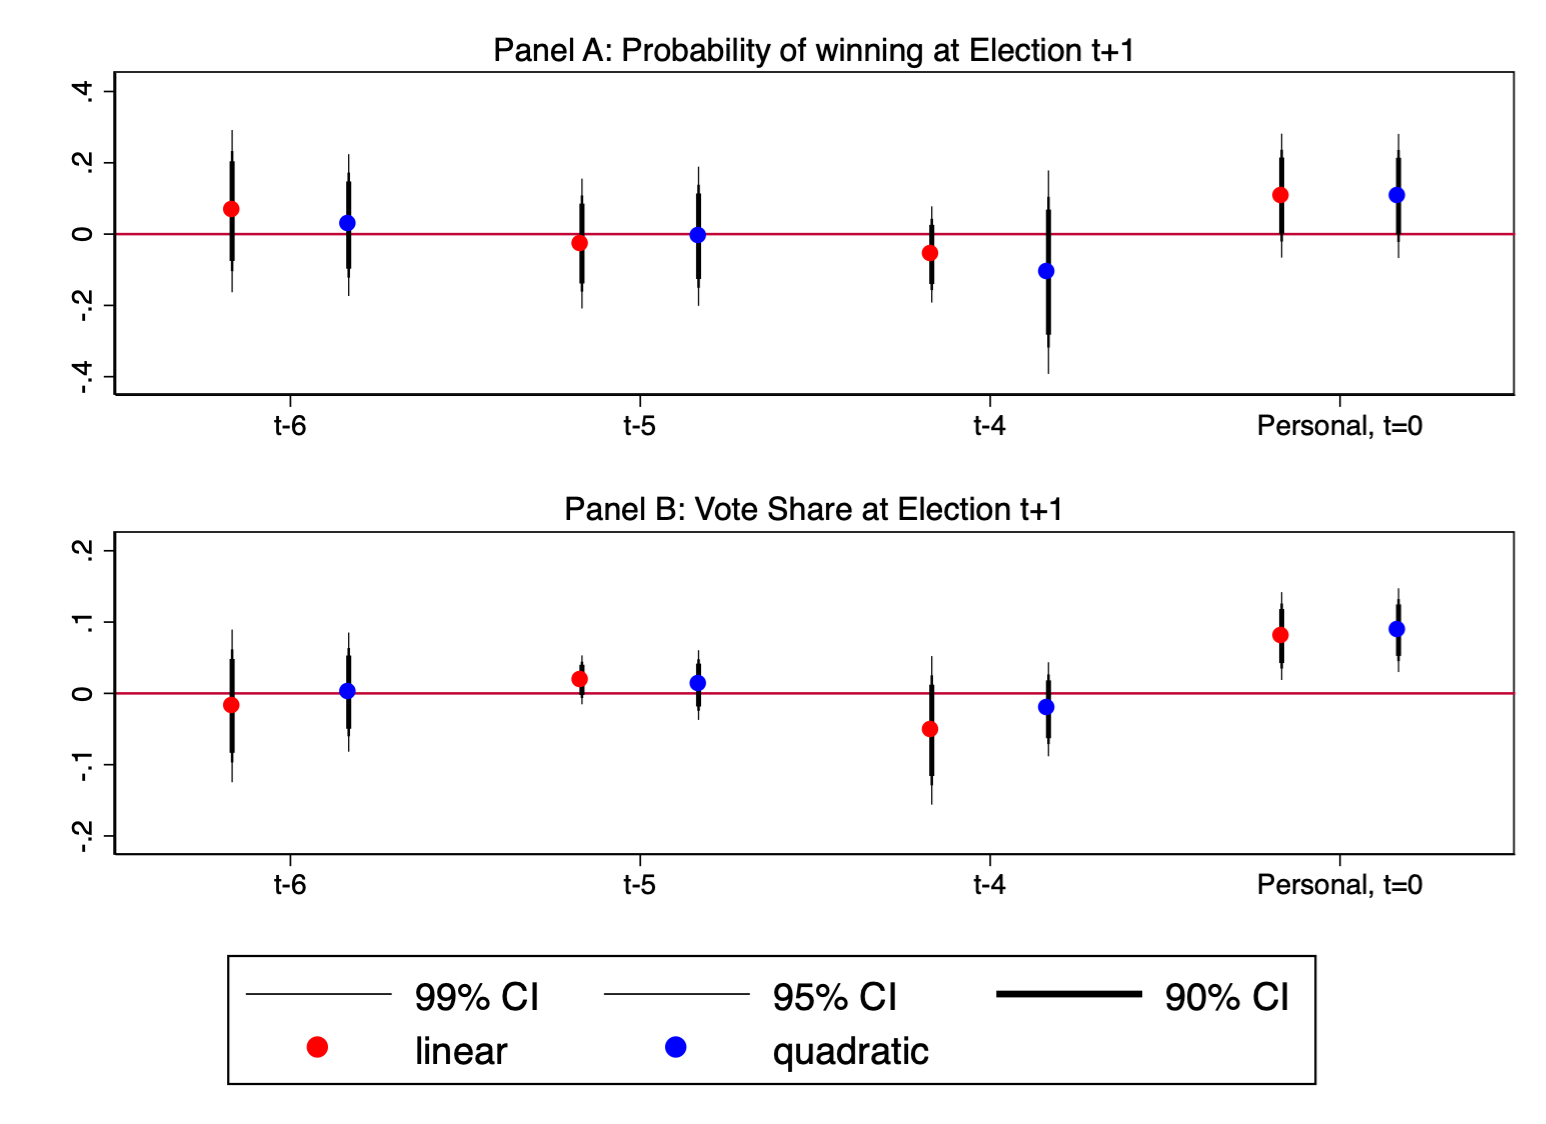
\includegraphics[width=0.9\textwidth]{Chapter2/Figures_incumbency/event_study.png}
       \captionsetup{justification=centering}
         
 \textbf{Note:} Figure \ref{fig:event_study_personal} shows the average difference-in-discontinuity estimator of the effect of the Term Limit Reform that compares municipalities with incumbents that barely won to those that barely lost in the election at $t$ on the probability of winning in the election at $t+1$ (Panel A) and the vote share in the  election at $t+1$ (Panel B). Optimal bandwidths following \citet{calonicoetal_2014} are used. 
  
\end{figure}  
 
    
\subsection{Robustness tests \label{sec:robustness}} 
  
To test the robustness of results I start by comparing the difference-in-discontinuity of close election design results from Table \ref{tab:naive_twfe} with the design used by \citet{fowler_hall_2014}. To estimate the personal and partisan incumbency advantages \citet{fowler_hall_2014} run two different regressions: first, a regression discontinuity design of close elections where candidates are prevented from running for reelection, i.e. they are term limited; second, a regression discontinuity design where candidates are non-term limited, i.e. they can run for reelection if desired. The difference between the estimated coefficients of these two models results in the personal incumbency advantage, while the first one estimates the partisan one and the second one the conjoint partisan and personal incumbency advantages. Results are then corrected by the probabilities of reelection attempts as described in Section \ref{sec:design_literature}. Table \ref{tab:fowler_hall} shows the partisan and personal incumbency advantages following \citet{fowler_hall_2014} using both the probability of victory as well as the winning margin in the next election as outcomes, and all mayoral elections in Mexico since 2000. Panel A shows the results using a linear polynomial while Panel B uses a quadratic one. Overall, we see that without term limits, in Mexico incumbents had a positive but non-significant incumbency advantage. However, term limited races show that a partisan incumbency disadvantage exists between -8 to -9\% depending on the specification. Contrastingly, the difference between the term limit and non-term limit cases in column (3) shows the personal incumbency returns to be positive and significant to the 1\% level. These results coincide with the asymmetry found in Table \ref{tab:naive_twfe}. The difference with the results from Table \ref{tab:naive_twfe}, however, is that for the results of Table \ref{tab:fowler_hall} to be identified we need to assume parallel trends hold.   

\begin{table}[htbp]\def\sym#1{\ifmmode^{#1}\else\(^{#1}\)\fi}
\centering
\caption{Personal and Partisan Incumbency Advantage following \citet{fowler_hall_2014}}
\label{tab:fowler_hall}
\scalebox{1}{
\begin{tabular}{lccc}
\hline \hline
& \multicolumn{3}{c}{\textbf{Panel A: linear polynomial}}\\
& \multicolumn{1}{c}{No term limits:} & \multicolumn{1}{c}{term limits:} & \multicolumn{1}{c}{difference:}\\
Advantage: & \multicolumn{1}{c}{personal + partisan} & \multicolumn{1}{c}{partisan} & \multicolumn{1}{c}{personal} \\
& \multicolumn{1}{c}{(1)} & \multicolumn{1}{c}{(2)} & \multicolumn{1}{c}{(3)} \\
\cmidrule(lrr){2-2}  \cmidrule(lrr){3-3} \cmidrule(lrr){4-4}\\
\addlinespace
RD estimate: prob(victory in t+1) &      $ 0.0568^{} $ &  $ -0.1269^{***} $  &  $ 0.1468^{***} $  \\
& ($ 0.0508$) & ($ 0.0208 $)  & ($ 0.0038 $)\\
RD estimate: vote share in t+1 &      $ 0.0245^{} $ &  $ -0.0529^{***} $  &  $ 0.0618^{***} $  \\
& ($ 0.0243$) & ($ 0.0073 $)  & ($ 0.0024 $)\\
\addlinespace
Observations: prob(victory in t+1)      &            1257        &     9180  \\
Observations: vote share in t+1      &            1221        &     8758  \\
\\
& \multicolumn{3}{c}{\textbf{Panel B: quadratic polynomial}}\\
& \multicolumn{1}{c}{No term limits:} & \multicolumn{1}{c}{term limits:} & \multicolumn{1}{c}{difference:}\\
Advantage: & \multicolumn{1}{c}{personal + partisan} & \multicolumn{1}{c}{partisan} & \multicolumn{1}{c}{personal} \\
& \multicolumn{1}{c}{(1)} & \multicolumn{1}{c}{(2)} & \multicolumn{1}{c}{(3)} \\
\cmidrule(lrr){2-2}  \cmidrule(lrr){3-3} \cmidrule(lrr){4-4}\\
\addlinespace
RD estimate: prob(victory in t+1) &      $ 0.0442^{} $ &  $ -0.1291^{***} $  &  $ 0.1384^{***} $  \\
& ($ 0.0676$) & ($ 0.0258 $)  & ($ 0.0042 $)\\
RD estimate: vote share in t+1 &      $ 0.0311^{} $ &  $ -0.0510^{***} $  &  $ 0.0656^{***} $  \\
& ($ 0.0274$) & ($ 0.0092 $)  & ($ 0.0026 $)\\
\addlinespace
Observations: prob(victory in t+1)      &            1257        &     9180  \\
Observations: vote share in t+1      &            1221        &     8758  \\
\hline \hline
\multicolumn{4}{p{1\textwidth}}{\footnotesize{Notes: Standard errors in parentheses are clustered at the state level, with the following significance-level: $^{***}$ 1\%; $^{**}$ 5\%; and $^*$ 10\%, that refer to two-sided t-test with the null hypothesis equal to 0 for each relative time period. Table estimated using all elections since the year 2000.}}
\end{tabular}
}
\end{table}
   


For robustness we also check whether results change by varying the bandwidth for close elections. Appendix Figure \ref{fig:bandwidths} shows this to be the case overall, with an asymmetry found between the partisan and personal incumbency advantages for the linear and quadratic specifications, using both the probability of winning or vote share in the election $t+1$.       


\section{Mechanisms: What explains the observed electoral returns from incumbency? \label{sec:mechanisms}}
           
A big concern of the literature has been understanding the determinants of incumbency advantage. To date, we can identify at least three broad types of explanations. First, what incumbents do (and opponents cannot do) emphasizing the resources, visibility, and power that incumbents gain from office holding \citep{mayhew_1974, fiorina_1989, king_1991, cox_morgensten_1993}.  Second, quality-based explanations that emphasize who incumbents are (and who their opponents are) \citep{cox_katz_1996, levitt_wolfram_1997, ansolabehere_snyder_2000, eggers_2017}. In this second line we find explanations related to incumbents’ quality as well as the “scare-off effect”, or the ability incumbents have to scare off high-quality challengers. A third and more recent type of mechanism emphasizes the role of information. \citet{ashworth_bdm_2008} find that incumbency advantage is dependent on how precise the information is about incumbent’s ability to voters. More recently, \citet{ashworth_etal_2019} expand on the role of information to explain incumbency advantage: through a theoretical model, they show that incumbents have an additional information advantage to challengers: they govern while challengers do not. This is so even absent any partisanship, electoral selection or challenger scare off. However, to date there is no empirical identification of the information-based explanation proposed by these authors. Moreover, if theoretical work done by Ashworth and co-authors is correct, all other explanations of incumbency advantage might be biased by the role information plays. 
 
To test if a resource-based incumbency advantage explains the returns observed in Section \ref{sec:results}, I evaluate the effect of the reform on municipal revenues and fiscal transfers. Local tax revenues have been used by the incumbency advantage literature to test whether a resourced-based incumbency advantage exists \citep{fiorina_1989, cox_morgensten_1993}. The most relevant tax revenues at the municipal level in Mexico are property and estate taxes. Two additional sources of local revenues are important, those coming from the ownership of vehicles (\emph{tenencia} in Spanish) as well as revenues from taxing new cars. Mayors tend to use these two sources of revenues to increase their treasury but are highly unapproved by voters. As a result, we would expect mayors with reelection incentives not to rely on these types of tax revenues. Table \ref{tab:revenues} Panel A shows that total municipal revenues increased by 44 million pesos significant to the 5\% level for mayors up for reelection and that barely won in the election at $t$ relative to those with term limits and barely lost at $t$.  This is true for the linear and quadratic specifications.\footnote{One dollar is equivalent to 20 pesos approximately.} This result represents an increase of a quarter of the mean of total municipal revenues. A large increase of municipal revenues comes from an increase in tax revenues (columns 3 and 4 of Panel A), particularly property tax revenues (columns 5 and 6), and estate tax revenues (columns 7 and 8). Null effects are found for production, consumption and transactions tax revenues in Panel B columns 1 and 2. Interestingly, unpopular taxes like the \emph{tenencia} decrease in revenues for mayors up for reelection and that barely won in election $t$ relative to those term limited and that barely lost in $t$. Now, the increase in municipal revenues is used as a measure of the increase in resources. The increase could be driven by an increase in the effort of tax collection, an increase in tax rates or better economic conditions that lead to higher tax revenues. For the case of municipal revenues in Mexico it is hard to disentangle between these three mechanisms, specially since there is no data on local tax rates or effort in tax collection. The main takeaway, however, is that municipalities with mayors up for reelection at that barely won their election at $t$ increase the amount of resources. As a result, voters create a resource-based incumbency advantage with the believe that they will receive a higher budget or transfer in the future. %%%rewrite .

 %\begin{landscape} 
 %REVENUES     
\begin{table}[htbp]\def\sym#1{\ifmmode^{#1}\else\(^{#1}\)\fi}
\centering
\caption{Revenues of Municipal Governments, Difference-in-Discontinuity of Close Elections Model}
\label{tab:revenues}
\scalebox{0.55}{ 
\begin{tabular}{l*{8}{c}}
\hline \hline 
\\
& \multicolumn{8}{c}{\textbf{Panel A:}}  \\


Dependent variable in million pesos$^b$: & \multicolumn{2}{c}{\begin{tabular}[c]{@{}c@{}}Total Municipal \\ Revenues\end{tabular}}  & \multicolumn{2}{c}{Tax Revenues} & \multicolumn{2}{c}{\begin{tabular}[c]{@{}c@{}}Property Tax \\ Revenues\end{tabular}} & \multicolumn{2}{c}{\begin{tabular}[c]{@{}c@{}}Estate Tax \\ Revenues\end{tabular}} \\
\cmidrule(lr){2-3}\cmidrule(lr){4-5}\cmidrule(lr){6-7}\cmidrule(lr){8-9}


             &\multicolumn{1}{c}{linear}&\multicolumn{1}{c}{quadratic}&\multicolumn{1}{c}{linear}&\multicolumn{1}{c}{quadratic}&\multicolumn{1}{c}{linear}&\multicolumn{1}{c}{quadratic}&\multicolumn{1}{c}{linear}&\multicolumn{1}{c}{quadratic}\\\cmidrule(lr){2-2}\cmidrule(lr){3-3}\cmidrule(lr){4-4}\cmidrule(lr){5-5}\cmidrule(lr){6-6}\cmidrule(lr){7-7}\cmidrule(lr){8-8}\cmidrule(lr){9-9}
            &\multicolumn{1}{c}{(1)}         &\multicolumn{1}{c}{(2)}         &\multicolumn{1}{c}{(3)}         &\multicolumn{1}{c}{(4)}         &\multicolumn{1}{c}{(5)}         &\multicolumn{1}{c}{(6)}         &\multicolumn{1}{c}{(7)}         &\multicolumn{1}{c}{(8)}         \\
\addlinespace
Term Limit Reform&    -32.2546\sym{***}&    -31.5521\sym{***}&      0.7710         &      0.8451         &      2.8797         &      3.0528         &     -1.5350         &     -1.4900         \\
            &   (10.0656)         &   (10.4937)         &    (2.8949)         &    (2.9493)         &    (2.4988)         &    (2.5249)         &    (2.7821)         &    (2.8250)         \\
\addlinespace
\begin{tabular}[c]{@{}l@{}} Dummy win, Election at t \end{tabular}&    -15.2045         &    -14.4905         &     -0.8681         &     -0.7554         &     -3.6883\sym{*}  &     -3.5814         &     -3.6395         &     -3.5547         \\
            &    (9.5364)         &    (8.9873)         &    (2.3791)         &    (2.4264)         &    (2.1232)         &    (2.1299)         &    (2.2483)         &    (2.2599)         \\
\addlinespace
\begin{tabular}[c]{@{}l@{}} Interaction: Reform X Win Election at t \end{tabular}&     44.2806\sym{**} &     44.9223\sym{**} &      7.1171\sym{**} &      7.4166\sym{**} &      6.3265\sym{**} &      6.4784\sym{**} &      9.2480\sym{**} &      9.3405\sym{**} \\
            &   (16.0947)         &   (16.3556)         &    (2.7790)         &    (2.8267)         &    (2.8047)         &    (2.8943)         &    (3.4478)         &    (3.5175)         \\
\addlinespace
Observations&        1352         &        1352         &        1366         &        1366         &         984         &         984         &        1170         &        1170         \\
R-squared   &       0.981         &       0.981         &       0.967         &       0.967         &       0.964         &       0.964         &       0.971         &       0.971         \\
Municipal FE&  \checkmark         &  \checkmark         &  \checkmark         &  \checkmark         &  \checkmark         &  \checkmark         &  \checkmark         &  \checkmark         \\
Year FE     &  \checkmark         &  \checkmark         &  \checkmark         &  \checkmark         &  \checkmark         &  \checkmark         &  \checkmark         &  \checkmark         \\
Controls$^a$&                     &                     &                     &                     &                     &                     &                     &                     \\
Polynomial  &      linear         &   quadratic         &      linear         &   quadratic         &      linear         &   quadratic         &      linear         &   quadratic         \\
Difference:Personal($\beta\_0$)-Partisan($\gamma\_0$)&$59.4850^{**}$         &$59.4128^{**}$         &$7.9852^{*}$         &$8.1720^{*}$         &$10.0149^{**}$         &$10.0599^{**}$         &$12.8876^{**}$         &$12.8952^{**}$         \\
SE (Difference)&     23.5860         &     23.3221         &      4.1091         &      4.0936         &      3.7193         &      3.7970         &      5.3087         &      5.3617         \\
Mean DV in million pesos$^b$&       190.6         &       190.6         &        23.3         &        23.3         &        15.0         &        15.0         &        21.4         &        21.4         \\
   
   
\\
& \multicolumn{8}{c}{\textbf{Panel B:}}  \\
\\
Dependent variable in million pesos$^b$: & \multicolumn{2}{c}{\begin{tabular}[c]{@{}c@{}}Prod., Cons. and \\ Trans. Tax Revenues \end{tabular}} & \multicolumn{2}{c}{\begin{tabular}[c]{@{}c@{}}Vehicle Ownership Tax \\ Revenues (\emph{Tenencia}) \end{tabular}}  & \multicolumn{2}{c}{\begin{tabular}[c]{@{}c@{}}New Cars Tax \\ Revenues \end{tabular}} \\
 \cmidrule(lr){2-3}\cmidrule(lr){4-5}\cmidrule(lr){6-7}

             &\multicolumn{1}{c}{linear}&\multicolumn{1}{c}{quadratic}&\multicolumn{1}{c}{linear}&\multicolumn{1}{c}{quadratic}&\multicolumn{1}{c}{linear}&\multicolumn{1}{c}{quadratic}\\\cmidrule(lr){2-2}\cmidrule(lr){3-3}\cmidrule(lr){4-4}\cmidrule(lr){5-5}\cmidrule(lr){6-6}\cmidrule(lr){7-7}
            &\multicolumn{1}{c}{(1)}         &\multicolumn{1}{c}{(2)}         &\multicolumn{1}{c}{(3)}         &\multicolumn{1}{c}{(4)}         &\multicolumn{1}{c}{(5)}         &\multicolumn{1}{c}{(6)}         \\
\addlinespace
Term Limit Reform&      6.8810         &      6.9335         &     -0.3763         &     -0.3717         &      0.1546\sym{**} &      0.1594\sym{**} \\
            &    (6.8291)         &    (6.8923)         &    (0.2705)         &    (0.2726)         &    (0.0723)         &    (0.0740)         \\
\addlinespace
\begin{tabular}[c]{@{}l@{}} Dummy win, Election at t \end{tabular}&      8.5129         &      8.5019         &      0.2589         &      0.2554         &     -0.0630         &     -0.0648         \\
            &    (9.0537)         &    (9.0607)         &    (0.1999)         &    (0.2046)         &    (0.1189)         &    (0.1203)         \\
\addlinespace
\begin{tabular}[c]{@{}l@{}} Interaction: Reform X Win Election at t \end{tabular}&     -8.6016         &     -8.5001         &     -1.0651\sym{**} &     -1.0659\sym{**} &      0.2978\sym{*}  &      0.2957\sym{*}  \\
            &    (8.8616)         &    (8.7694)         &    (0.4581)         &    (0.4602)         &    (0.1628)         &    (0.1606)         \\
\addlinespace
Observations&         409         &         409         &        1043         &        1043         &        1317         &        1317         \\
R-squared   &       0.521         &       0.521         &       0.658         &       0.658         &       0.969         &       0.969         \\
Municipal FE&  \checkmark         &  \checkmark         &  \checkmark         &  \checkmark         &  \checkmark         &  \checkmark         \\
Year FE     &  \checkmark         &  \checkmark         &  \checkmark         &  \checkmark         &  \checkmark         &  \checkmark         \\
Controls$^a$&                     &                     &                     &                     &                     &                     \\
Polynomial  &      linear         &   quadratic         &      linear         &   quadratic         &      linear         &   quadratic         \\
Difference:Personal($\beta\_0$)-Partisan($\gamma\_0$)&$-17.1145^{}$         &$-17.0020^{}$         &$-1.3240^{**}$         &$-1.3212^{**}$         & $0.3608^{}$         & $0.3605^{}$         \\
SE (Difference)&     17.8925         &     17.8078         &      0.6052         &      0.6123         &      0.2718         &      0.2703         \\
Mean DV in million pesos$^b$&         1.6         &         1.6         &         0.6         &         0.6         &         0.9         &         0.9         \\
   
    
        
\hline \hline 
\multicolumn{9}{p{1.6\textwidth}}{\footnotesize{Notes: Standard errors in parentheses are clustered at the state level. Significance-level: $^{***}$ 1\%; $^{**}$ 5\%; and $^*$ 10\%, that refer to two-sided t-test.$^a$ Pretreatment controls include: governor winning margin; party alignment with the President;  party alignment with the Governor; and logged population. $^b$ 1 dollar = 20 pesos approximately. Thus, 1 million pesos are \$200,000 USD.}} \\
\end{tabular}
}.  
\end{table}    
%\end{landscape}   
        

 Besides revenues, we can use data on municipal transfers from the federation or the state to proxy for resources. These transfers can be divided into two types: ear-marked and not ear-marked. Ear-marked transfers are those which are determined mostly by the use of fiscal formulas and are targeted to specific ``ear-marked'' expenses or conditional on certain activities. The most prominent municipal transfer in Mexico are the Federal and State Contributions Fund. Not ear-marked transfers are those that municipalities can exercise freely and are generally not audited by Federal Superior Audit in Mexico. The most prominent ones include the General Participation Fund as well as secondary participating funds. Other not ear-marked municipal transfers are the Municipal Development Fund, the Contribution Fund to Strengthen Municipalities and the Contribution Fund for Municipal Social Infrastructure. Table \ref{tab:transfers} shows the effect of the Term Limit Reform on these transfers. We see an increase of participations (columns 1-4 in Panel A), as well as contributions to municipal social infrastructure (columns 3 and 4 in Panel B)  in municipalities where mayors can run for reelection and barely won in election $t$ relative to those that are term limited and barely lost in election $t$. In contrast, no effects are found for ear-marked transfers, mainly the Federal and State Contributions. 
   
        
 %\begin{landscape}  
 %TRANSFERS    
\begin{table}[htbp]\def\sym#1{\ifmmode^{#1}\else\(^{#1}\)\fi}
\centering
\caption{Transfers to Municipal Governments from the Federation and the State, Difference-in-Discontinuity of Close Elections Model}
\label{tab:transfers}
\scalebox{0.6}{ 
\begin{tabular}{l*{6}{c}}
\hline \hline 
\\
& \multicolumn{6}{c}{\textbf{Panel A:}}  \\

        
Dependent variable in million pesos$^b$: & \multicolumn{2}{c}{\begin{tabular}[c]{@{}c@{}}General Participation \\ Fund\end{tabular}}  & \multicolumn{2}{c}{Participating Funds} & \multicolumn{2}{c}{\begin{tabular}[c]{@{}c@{}}Municipal Development \\ Fund\end{tabular}}  \\
\cmidrule(lr){2-3}\cmidrule(lr){4-5}\cmidrule(lr){6-7}
             &\multicolumn{1}{c}{linear}&\multicolumn{1}{c}{quadratic}&\multicolumn{1}{c}{linear}&\multicolumn{1}{c}{quadratic}&\multicolumn{1}{c}{linear}&\multicolumn{1}{c}{quadratic}\\\cmidrule(lr){2-2}\cmidrule(lr){3-3}\cmidrule(lr){4-4}\cmidrule(lr){5-5}\cmidrule(lr){6-6}\cmidrule(lr){7-7}
            &\multicolumn{1}{c}{(1)}         &\multicolumn{1}{c}{(2)}         &\multicolumn{1}{c}{(3)}         &\multicolumn{1}{c}{(4)}         &\multicolumn{1}{c}{(5)}         &\multicolumn{1}{c}{(6)}         \\
\addlinespace
Term Limit Reform&     -3.7726         &     -3.7781         &     -0.1525         &      0.0139         &      0.2237         &      0.2140         \\
            &    (3.1636)         &    (3.1626)         &    (3.2576)         &    (3.3629)         &    (0.4757)         &    (0.4772)         \\
\addlinespace
\begin{tabular}[c]{@{}l@{}} Dummy win, Election at t \end{tabular}&     -0.6749         &     -0.6681         &      0.4634         &      0.6110         &      0.0366         &      0.0509         \\
            &    (2.2195)         &    (2.2276)         &    (2.7421)         &    (2.7506)         &    (0.5091)         &    (0.5186)         \\
\addlinespace
\begin{tabular}[c]{@{}l@{}} Interaction: Reform X Win Election at t \end{tabular}&      6.6213\sym{**} &      6.6825\sym{**} &      8.0174\sym{**} &      8.3615\sym{**} &      0.8701         &      0.8906         \\
            &    (2.8621)         &    (2.7983)         &    (3.3955)         &    (3.4249)         &    (0.6735)         &    (0.6753)         \\
\addlinespace
Observations&        1317         &        1317         &        1285         &        1285         &        1138         &        1138         \\
R-squared   &       0.981         &       0.981         &       0.976         &       0.976         &       0.986         &       0.986         \\
Municipal FE&  \checkmark         &  \checkmark         &  \checkmark         &  \checkmark         &  \checkmark         &  \checkmark         \\
Year FE     &  \checkmark         &  \checkmark         &  \checkmark         &  \checkmark         &  \checkmark         &  \checkmark         \\
Controls$^a$&                     &                     &                     &                     &                     &                     \\
Polynomial  &      linear         &   quadratic         &      linear         &   quadratic         &      linear         &   quadratic         \\
Difference:Personal($\beta\_0$)-Partisan($\gamma\_0$)& $7.2962^{}$         & $7.3506^{}$         & $7.5540^{}$         & $7.7505^{}$         & $0.8335^{}$         & $0.8397^{}$         \\
SE (Difference)&      4.5115         &      4.4352         &      4.9473         &      4.9230         &      0.9980         &      1.0088         \\
Mean DV in million pesos$^b$&        41.5         &        41.5         &        54.7         &        54.7         &        10.0         &        10.0         \\
   

\\
& \multicolumn{6}{c}{\textbf{Panel B:}}  \\
\\
Dependent variable in million pesos$^b$: & \multicolumn{2}{c}{\begin{tabular}[c]{@{}c@{}}Contributions Fund to \\ Strengthen Municipalities \end{tabular}} & \multicolumn{2}{c}{\begin{tabular}[c]{@{}c@{}}Contribution Fund for \\ Municipal Social Infrastructure \end{tabular}}  & \multicolumn{2}{c}{\begin{tabular}[c]{@{}c@{}}Federal and State \\ Contributions \end{tabular}} \\
 \cmidrule(lr){2-3}\cmidrule(lr){4-5}\cmidrule(lr){6-7}

             &\multicolumn{1}{c}{linear}&\multicolumn{1}{c}{quadratic}&\multicolumn{1}{c}{linear}&\multicolumn{1}{c}{quadratic}&\multicolumn{1}{c}{linear}&\multicolumn{1}{c}{quadratic}\\\cmidrule(lr){2-2}\cmidrule(lr){3-3}\cmidrule(lr){4-4}\cmidrule(lr){5-5}\cmidrule(lr){6-6}\cmidrule(lr){7-7}
            &\multicolumn{1}{c}{(1)}         &\multicolumn{1}{c}{(2)}         &\multicolumn{1}{c}{(3)}         &\multicolumn{1}{c}{(4)}         &\multicolumn{1}{c}{(5)}         &\multicolumn{1}{c}{(6)}         \\
\addlinespace
Term Limit Reform&     -0.7954         &     -0.7805         &      0.7868         &      0.8159         &    -16.8333\sym{**} &    -16.5883\sym{**} \\
            &    (1.4516)         &    (1.4718)         &    (1.4226)         &    (1.3971)         &    (6.6819)         &    (6.7282)         \\
\addlinespace
\begin{tabular}[c]{@{}l@{}} Dummy win, Election at t \end{tabular}&     -0.0917         &     -0.0267         &     -1.4125         &     -1.4166         &     -3.9379         &     -3.8393         \\
            &    (1.0806)         &    (1.1145)         &    (1.7105)         &    (1.7182)         &    (4.4769)         &    (4.4217)         \\
\addlinespace
\begin{tabular}[c]{@{}l@{}} Interaction: Reform X Win Election at t \end{tabular}&      1.1915         &      1.2527         &      2.9133\sym{**} &      2.8935\sym{**} &     21.9864         &     22.1860         \\
            &    (1.9003)         &    (1.8980)         &    (1.4145)         &    (1.4071)         &   (13.0689)         &   (13.1533)         \\
\addlinespace
Observations&        1264         &        1264         &        1554         &        1554         &        1367         &        1367         \\
R-squared   &       0.980         &       0.980         &       0.881         &       0.881         &       0.894         &       0.894         \\
Municipal FE&  \checkmark         &  \checkmark         &  \checkmark         &  \checkmark         &  \checkmark         &  \checkmark         \\
Year FE     &  \checkmark         &  \checkmark         &  \checkmark         &  \checkmark         &  \checkmark         &  \checkmark         \\
Controls$^a$&                     &                     &                     &                     &                     &                     \\
Polynomial  &      linear         &   quadratic         &      linear         &   quadratic         &      linear         &   quadratic         \\
Difference:Personal-Partisan& $1.2832^{}$         & $1.2794^{}$         & $4.3259^{}$         & $4.3102^{}$         &$25.9243^{}$         &$26.0253^{}$         \\
SE (Difference)&      2.4246         &      2.4334         &      2.7656         &      2.7539         &     15.7681         &     15.8106         \\
Mean DV in million pesos$^b$&        25.3         &        25.3         &        21.4         &        21.4         &        68.6         &        68.6         \\
   
 
      
\hline \hline 
\multicolumn{7}{p{1.55\textwidth}}{\footnotesize{Notes: Standard errors in parentheses are clustered at the state level. Significance-level: $^{***}$ 1\%; $^{**}$ 5\%; and $^*$ 10\%, that refer to two-sided t-test.$^a$ Pretreatment controls include: governor winning margin; party alignment with the President;  party alignment with the Governor; and logged population. $^b$ 1 dollar = 20 pesos approximately. Thus, 1 million pesos are \$200,000 USD.}} \\
\end{tabular}
}
\end{table}  
%\end{landscape}      


Both transfers and revenues are used to proxy for measures of the resources incumbents may get and may affect their reelection chances or that of their parties. This is called the resource-based incumbency advantage where citizens create a positive incumbency return expecting a higher budget or transfer in the future \citep{cox_morgensten_1993}. The literature has also used measures of casework services to constituents or the ability to expand the bureaucracy and thus public labor to test for a resource based incumbency advantage \citep{cox_katz_1996}. I rely on data from the Municipal Government Census (\emph{Censos de Gobierno Municipal}) from 2011 to 2019 which collect information on the number of bureaucrats of municipalities, as well as the number of city council sessions, the number of approved initiatives of law and the percentage of municipal budget spend, all in the year prior to the census. This data spans from 2010 to 2018 every two years. For the case of Mexico, council sessions and initiatives approved is performed by the local council members (\emph{regidores}) who are elected by proportional representation in mayoral elections according to the vote received by the mayor. As such, they work directly with the mayor and can be considered as his bureaucrats specially when they belong to the same party. Table \ref{tab:effort} shows the effect of the 2014 Term Limit Reform on these  measures. We find no difference in the difference-in-discontinuity estimator of the number of city council sessions (Panel A columns 1 and 2), approved initiatives of law (Panel A columns 3 and 4), the municipal budget spend (Panel B columns 1 and 2) nor the number of bureaucrats (Panel B columns 3 and 4). While this results do not provide evidence on the resource-based incumbency advantage, the increase in transfes and revenues does. 
   
%EFFORT     
\begin{table}[htbp]\def\sym#1{\ifmmode^{#1}\else\(^{#1}\)\fi}
\centering
\caption{Effort by Mayors and their Bureaucracy, Difference-in-Discontinuity of Close Elections Model}
\label{tab:effort}
\scalebox{0.7}{ 
\begin{tabular}{l*{4}{c}}
\hline \hline 
\\
 
& \multicolumn{4}{c}{\textbf{Panel A:}}  \\
    
Dependent variable: & \multicolumn{2}{c}{\begin{tabular}[c]{@{}c@{}}Number of City \\ Council Sessions\end{tabular}}  & \multicolumn{2}{c}{\begin{tabular}[c]{@{}c@{}}Number of Approved \\ Initiatives of Law \end{tabular}} \\
\cmidrule(lr){2-3}\cmidrule(lr){4-5}

             &\multicolumn{1}{c}{linear}&\multicolumn{1}{c}{quadratic}&\multicolumn{1}{c}{linear}&\multicolumn{1}{c}{quadratic}\\\cmidrule(lr){2-2}\cmidrule(lr){3-3}\cmidrule(lr){4-4}\cmidrule(lr){5-5}
            &\multicolumn{1}{c}{(1)}         &\multicolumn{1}{c}{(2)}         &\multicolumn{1}{c}{(3)}         &\multicolumn{1}{c}{(4)}         \\
\addlinespace
Term Limit Reform&      2.4689         &      2.5518         &     -7.3600         &     -6.7344         \\
            &    (2.9919)         &    (3.0229)         &    (5.4889)         &    (5.1441)         \\
\addlinespace
\begin{tabular}[c]{@{}l@{}} Dummy win, Election at t \end{tabular}&      1.7484         &      1.7493         &     -5.8498\sym{**} &     -5.5670\sym{**} \\
            &    (1.4732)         &    (1.4642)         &    (2.4317)         &    (2.4724)         \\
\addlinespace
\begin{tabular}[c]{@{}l@{}} Interaction: Reform X Win Election at t \end{tabular}&     -0.4498         &     -0.5256         &     -7.0331         &     -7.5107         \\
            &    (3.2193)         &    (3.2117)         &    (6.5863)         &    (6.3834)         \\
\addlinespace
Observations&        1583         &        1583         &         248         &         248         \\
R-squared   &       0.634         &       0.634         &       0.578         &       0.580         \\
Municipal FE&  \checkmark         &  \checkmark         &  \checkmark         &  \checkmark         \\
Year FE     &  \checkmark         &  \checkmark         &  \checkmark         &  \checkmark         \\
Controls$^a$&                     &                     &                     &                     \\
Polynomial  &      linear         &   quadratic         &      linear         &   quadratic         \\
Difference:Personal-Partisan&$-2.1982^{}$         &$-2.2749^{}$         &$-1.1834^{}$         &$-1.9437^{}$         \\
SE (Difference)&      4.4795         &      4.4624         &      6.3721         &      6.0607         \\
Mean DV in million pesos$^b$&        24.8         &        24.8         &        17.8         &        17.8         \\
   
\\
& \multicolumn{4}{c}{\textbf{Panel B:}}  \\

Dependent variable: & \multicolumn{2}{c}{\begin{tabular}[c]{@{}c@{}}Municipal Budget Spend \\ (\%)\end{tabular}} & \multicolumn{2}{c}{\begin{tabular}[c]{@{}c@{}}Bureaucrats per \\ 100,000 inh.\end{tabular}} \\
\cmidrule(lr){2-3}\cmidrule(lr){4-5}
 
             &\multicolumn{1}{c}{linear}&\multicolumn{1}{c}{quadratic}&\multicolumn{1}{c}{linear}&\multicolumn{1}{c}{quadratic}\\\cmidrule(lr){2-2}\cmidrule(lr){3-3}\cmidrule(lr){4-4}\cmidrule(lr){5-5}
            &\multicolumn{1}{c}{(1)}         &\multicolumn{1}{c}{(2)}         &\multicolumn{1}{c}{(3)}         &\multicolumn{1}{c}{(4)}         \\
\addlinespace
Term Limit Reform&    -23.6191\sym{***}&    -23.6688\sym{***}&   -825.9573\sym{**} &   -796.6090\sym{**} \\
            &    (6.9436)         &    (6.9324)         &  (305.4635)         &  (298.4410)         \\
\addlinespace
\begin{tabular}[c]{@{}l@{}} Dummy win, Election at t \end{tabular}&      0.2296         &      0.1382         &     48.6010         &     59.6989         \\
            &    (2.3315)         &    (2.4940)         &  (188.6225)         &  (177.3607)         \\
\addlinespace
\begin{tabular}[c]{@{}l@{}} Interaction: Reform X Win Election at t \end{tabular}&      2.2512         &      2.5769         &      5.1642         &    -20.0085         \\
            &    (4.2636)         &    (4.3070)         &  (400.3438)         &  (386.5135)         \\
\addlinespace
Observations&         262         &         262         &         434         &         434         \\
R-squared   &       0.641         &       0.642         &       0.862         &       0.862         \\
Municipal FE&  \checkmark         &  \checkmark         &  \checkmark         &  \checkmark         \\
Year FE     &  \checkmark         &  \checkmark         &  \checkmark         &  \checkmark         \\
Controls$^a$&                     &                     &                     &                     \\
Polynomial  &      linear         &   quadratic         &      linear         &   quadratic         \\
Difference:Personal($\beta\_0$)-Partisan($\gamma\_0$)& $2.0216^{}$         & $2.4387^{}$         &$-43.4368^{}$         &$-79.7074^{}$         \\
SE (Difference)&      5.6436         &      5.8323         &    559.3015         &    534.5561         \\
Mean DV in million pesos$^b$&        11.1         &        11.1         &      1685.8         &      1685.8         \\
   
     
\hline \hline 
\multicolumn{5}{p{1\textwidth}}{\footnotesize{Notes: Standard errors in parentheses are clustered at the state level. Significance-level: $^{***}$ 1\%; $^{**}$ 5\%; and $^*$ 10\%, that refer to two-sided t-test.$^a$ Pretreatment controls include: governor winning margin; party alignment with the President;  party alignment with the Governor; and logged population.}} \\
\end{tabular}
} 
\end{table}      
%\end{landscape}   
 

 \begin{figure}[H]   
\centering
 \caption{Effect of Term Limit Reform on the Quality of Candidates}
 \label{fig:quality_trend}
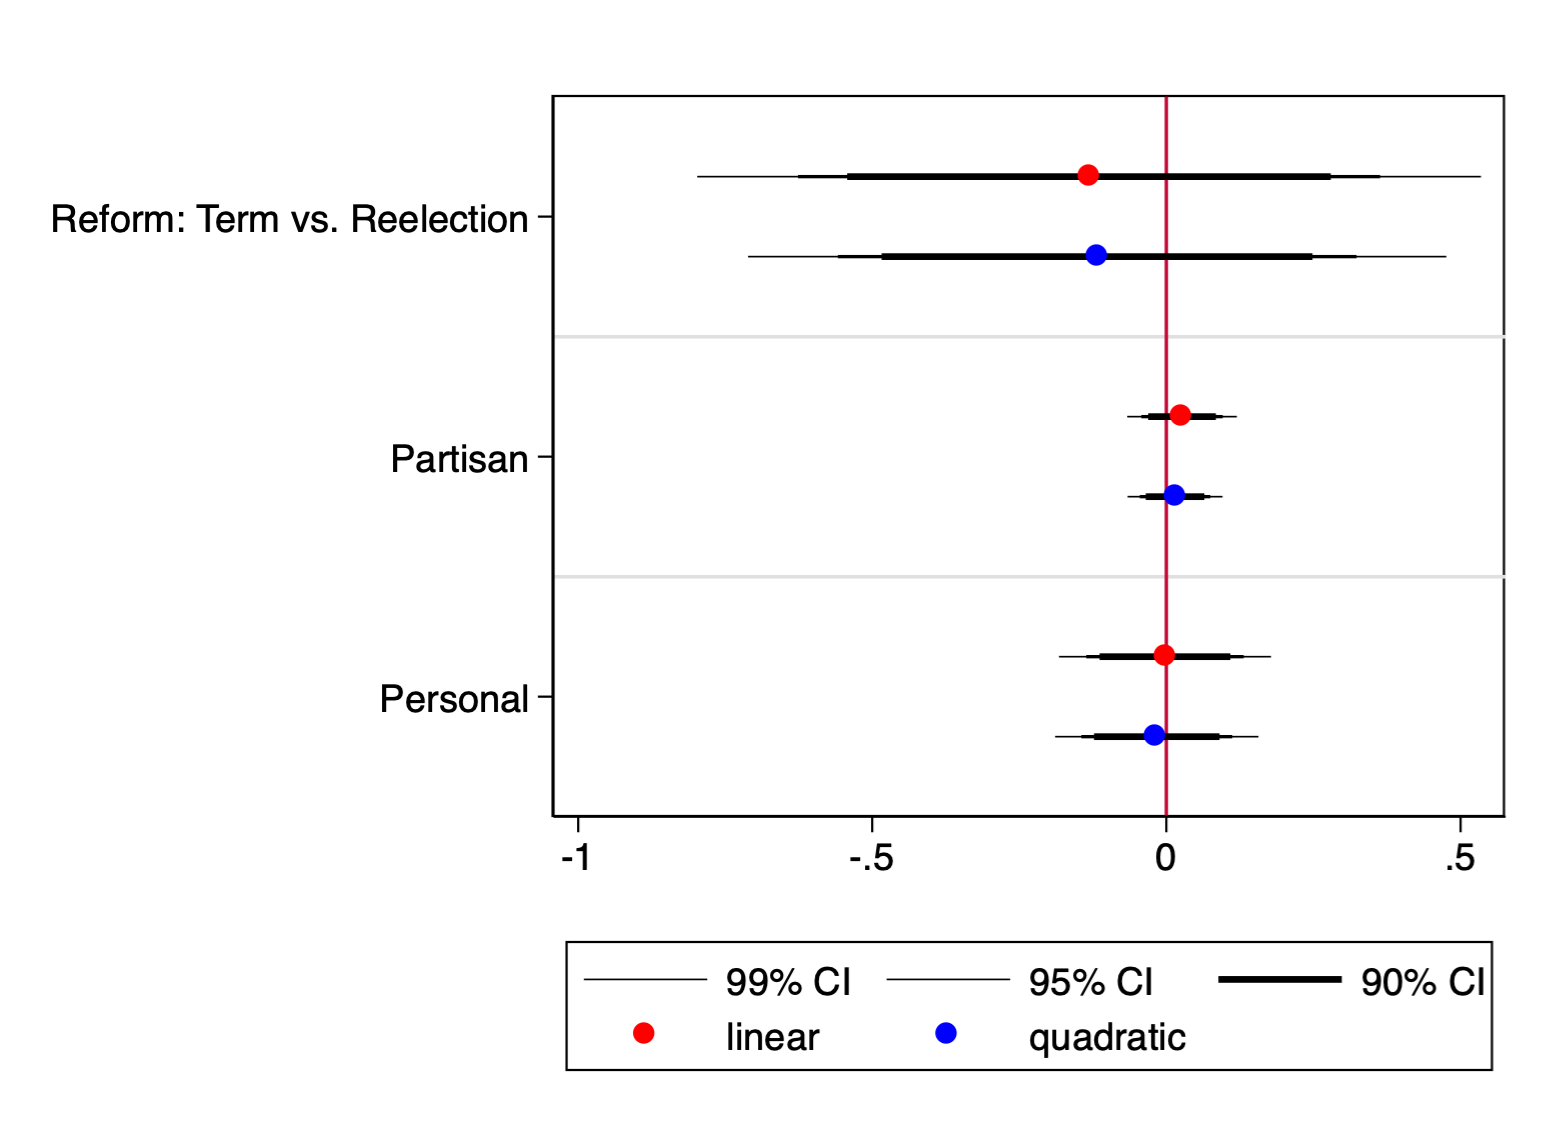
\includegraphics[width=0.9\textwidth]{Chapter2/Figures_incumbency/quality.png}
       \captionsetup{justification=centering}
         
 \textbf{Note:} Figure \ref{fig:quality_trend} shows the average treatment effect of the Term Limit Reform on a dummy indicator of whether candidates hold a professional title. Same optimal bandwidths as those in Table \ref{tab:naive_twfe} are used, as well as the same number of observations.   
     
\end{figure}   

To test for a quality-based incumbency advantage, Figure \ref{fig:quality_trend} shows the difference-in-discontinuity estimator on the indicator of whether a mayor hold a professional title, i.e. the coefficient for the personal incumbency advantage. We observe no difference in the quality of incumbents that barely won the election in $t$ to those that barely lost, before and after the Electoral Reform. In other words, it seems there is no evidence of a quality-based incumbency advantage. However, there could exist a difference in the quality of challengers who out of fear to the experience and ability of incumbents might choose not to run for office, the so called scare-off effect. Sadly, there is no municipal level data on the quality of challengers. To test for potential scare-off effects we would have to compare either a term-limited mayor who was won election once to a term-limited mayor who has won election twice, where both are facing the same election incentives but hold different selection histories. The same could be done by comparing first term mayor that can reelection and has won election once to a mayor that can reelect and has won election twice. This experiment to isolate the election from the selection effect is done by \citet{ashworth_2012}. We leave this test for future research.

Lastly, these estimates do not allow to test for an information-based incumbency advantage. To do so we would need data on whether citizens increased their information reception of incumbents actions and behavior in office. Future work is needed to disentangle the specific information and quality-based mechanisms behind the observed incumbency returns in mayoral elections in Mexico. 

  

\section{Conclusion} 

This paper disentangles the partisan from the personal incumbency advantages. By not disentangling these two components when estimating incumbency electoral returns, most of the literature has failed to correctly identify the valuation citizens have on the electoral system and the existent accountability relationships between parties, politicians and voters. To unbox incumbency advantage into its personal and partisan components, this paper relies on a difference-in-discontinuity of close elections design that exploits the staggered implementation of the 2014 Electoral Reform in Mexico that removed term limits for local mayors. In a setting of close elections, term limit mayors allows us to identify the partisan incumbency returns, while those up for reelection identify both the partisan and personal returns. The difference between these two measures allows for the identification of the personal incumbency advantage. Moreover, the difference-in-difference setup allows us to test for no differential trends of these two type of races prior to the introduction of the reform, while the regression discontinuity of close elections design allows us to reduce the potential of omitted variables, including party, elections and candidates differences. Lastly, we consider only mayors in their first terms which allows us to leave aside selection concerns coming from differences in experience and skills. 

The main result of the paper shows that the implementation of reelection in Mexico led to an incumbency advantage. However, this incumbency advantage can be decomposed into a personal incumbency \emph{advantage} and a partisan incumbency  \emph{disadvantage}. Since the personal incumbency advantage is greater than the partisan incumbency disadvantage, results suggest that reelection makes incumbency a personal affair and may signal a potential party dealignment in Mexican politics. The asymmetric effects also imply parties in Mexico do not hold a credible threat to punish renegade non-term limit mayors any longer. 

The paper further tries to explain the reasons behind the observed incumbency returns. An increase in the revenues and fiscal transfers to municipalities provide strong evidence of a resource-based incumbency advantage. In other words, citizens create a positive incumbency return with candidates who they expect will bring a higher budget or transfer in the future, and not their parties. We also test whether a quality-incumbency advantage exists. While no quality differences are found between term limit and non-term limit incumbents before and after the implementation of the Term Limit Reform, more data is needed to test for potential scare-off effects. It is also important to note that we do not have data on whether citizens increased their information reception of incumbents action, data that could be used to test whether an information-based incumbency advantage explains the observed results.


%
\chapter{Endogenous taxation in ongoing internal conflict: The case of Colombia}\footnote{This chapter was coauthored with Jacob Shapiro (Princeton University), Abbey Steele (University of Amsterdam) and Juan F. Vargas (Universidad El Rosario). The chapter was published in the American Political Science Review in 2018, Volume 112, Issue 4, pp. 996 - 1015.} 

\section{Introduction}

Historically, conflicts have motivated states to develop their fiscal capacity. According to \citet{tilly92a}, the formation of nation-states in early modern Europe emerged in part by the fiscal demands created by expansionary external wars. Those demands incentivized leaders to develop institutions that could monitor local populations and levy taxes. The resulting tax revenue was used to finance armies that would protect their kingdoms from external threats or expand their territories. Subsequent work provides empirical support for this theory at the cross-country level \citep{besleypersson08a} and refines it for regions outside of Europe \citep{centeno03a, vu10b} and for more recent time periods \citep{schevestasavage12a}.\footnote{Despite broad support for the theory, some have challenged its validity for early modern Europe \citep[e.g.,][]{spruyt96a, ertman97a, gorski93a}.} 

Yet the effect of \textit{internal} wars on statebuilding and fiscal capacity is more ambiguous. While an extension of Tilly's logic to internal wars implies that the state should try harder to state-build when challenged, that clearly does not always happen. This rasies an important question: what prevents would-be contemporary state-builders from acting on these incentives? Of course, when two parties are seeking to build competing tax institutions within the same territory (e.g. state and rebels), then the net effect is ambiguous. \citet{centeno03a} also argues that the prevalence of civil wars rather than mass wars in Latin America accounts for the weaker states in the region, because they fostered elite divisions, physical destruction and military rather than mass mobilization. 

Empirically, \citet{besleypersson08a} and \citet{cardenaseslava14a} provide evidence that internal conflict negatively affects various measures of state capacity. In Southeast Asia, however, \citet{slater10a} finds that communal urban unrest and endemic violence are both likely to lead elites to tax themselves. And in Latin America, \citet{soifer15a} finds evidence that the prevalence of conflict was crucial for extending the state during the 19\textsuperscript{th} century, and \citet{rodriguez-franco16a} finds that Colombia's elites in Bogot\'{a} began  to support statebuilding through new taxes in the early 2000s after several decades of internal conflict.  
  
The literature has so far focused on national-level fiscal capacity, but contemporary states feature multiple administrative layers, and a critical ingredient for the consolidation of the state is the introduction of sound and efficient tax systems at the local level. Moreover, security provision, property rights protections and a variety of development projects at the local level could, in theory, facilitate state-building by shaping citizens' preferences and behavior in ways that favor the state over its competitors. 

Several potential mechanisms have been proposed to explain the relationship between internal conflict and state capacity that are relevant for thinking about the relationship between conflict and tax performance at the local level. To mention a few: (1) By destroying physical capital, inducing forced migration and reducing the market value of private property in affected areas, conflict deteriorates the tax base; (2) Conflict generates negative reciprocity of tax payers towards a state that they judge to have failed to protect them \citep{cardenaseslava14a}; (3) A conflict environment reduces the return of productive activities and raise that of illegal businesses, which do not pay taxes to the state \citep{besleypersson08a}; (4) Armed groups create their own governance systems that divert civilians' resources away from the state and crowd out state institutions \citep{mampilly11a, arjona16a, sanchez-de-la-sierra17a}; and (5) Conflict facilitates the emergence of interest groups with {\it de facto} power (for instance because of their access to weapons) that can capture local political and economic institutions \citep{eaton06a, lopez10a, mampilly11a}. Such capture prevents state institutions from eliminating competitors, and from creating a durable and credible relationship with citizens in these regions.

We focus on the latter political economy mechanism. In the context of internal conflicts local tax institutions (both formal and informal) are shaped by different types of vested interests. We explore the extent to which armed groups shape existing property and tax institutions \textit{differently} depending on their preferences. To the best of our knowledge, this mechanism has not been studied in the previous literature, either theoretically or empirically.\footnote{See \citet{eaton06a} and \citet{lopez10a} on other forms of capture by illegal armed groups in Colombia. \citet{mampilly11a} analyzes rebel governance more broadly and \citet{arjona14a} finds that armed groups operated alongside state institutions in roughly one-quarter of the Colombian communities in her sample.} Our argument is that local tax and property rights institutions are shaped by illegal armed actors who influence state institutions to further their interests and those of the civilian groups they favor. Specifically, we expect that right-wing paramilitary groups will favor establishing formal property rights for land owners, while left-wing insurgents will do the opposite.

We test this argument in Colombia, which has four traits that make it an ideal setting for studying the relationship between civil conflict, institutional capture and local tax performance. First, the dynamics of the internal conflict vary substantially across the country's 1,122 municipalities. Moreover, within each municipality violence also varies across different periods of the war.  Second, Colombia sits roughly in the middle of the distribution of non-OECD countries in terms of the share of tax revenues generated locally \citep{deMello2000}.\footnote{The share of tax revenue collected locally is the standard measure of revenue decentralization in the literature, but is only available for a limited subset of countries.} It also ranks in the middle of large developing countries in terms of local revenue mobilization, above Indonesia at ~38\% but below India at approximately 62\% \citep{bird2012}. Third, local government authorities have substantial freedom to shape property and tax institutions. They can choose tax rates, order or impede updates on the land value, select revenue collection methods, and alter penalties and incentives. In theory, this autonomy could facilitate efficient local tax administration by allowing the system to be tailored to the needs of each municipality. In practice, in the context of uneven state presence and varying degrees of contestation by illegal armed groups, local institutions can be captured by private groups with vested interests.\footnote{This insight follows naturally from the theory in \citet{perssontabellini02a}, among others, in which heterogeneous agents take advantage of the discretion granted them.} 

Fourth, and most importantly, the main combatants had clear preferences regarding state-backed property rights throughout much of the war, which had implications for the local tax base and performance. Right-wing paramilitaries favored land owners, and promoted the accumulation of large estates which served as means to launder illegally acquired capital (through the drug trade, for example) or realize economies of scale in agricultural production and cattle ranching \citep{reyes07a}.\footnote{Paramilitaries displaced people to take their land and titling in areas with paramilitary presence was not always above-board. For example, public notaries, the officials charged with validating the provenance of land, were infiltrated by paramilitaries \citep[e.g.,][]{duran12a, verdad-abierta12a}.} 
On the left-wing side, both FARC and ELN guerrilla groups aimed to replace what they characterized as an unjust state and claimed to be acting on behalf of peasants and workers. The guerrillas backed land invasions of state and private property in many areas \citep[e.g.,][]{steele17a}. The FARC also viewed state-recognized private property as illegitimate or unnecessary: in its VIII Conference in 1993, it still backed collectivized property \citep{bernal-morales14a}. (During peace talks with the Santos administration in 2012, the FARC supported land formalization for the first time.) In areas that they influenced, the guerrillas regulated property in parallel to the state. For instance, they claimed the right to redistribute unused land or land from narcotraffickers \citep{bernal-morales14a}.\footnote{Internal divisions with the FARC existed, but it was a centralized organization that adopted policies in its Conferences that were relatively well enforced throughout. The paramilitaries were more decentralized but none challenged the basic legitimacy of state institutions (even if they argued that they could be run more effectively) \citep{gutierrez-sanin08a,romero03a}.} 

These positions on property rights stem from ideological commitments and make sense from the perspective of combatants trying to maximize their control over territory, and to mobilize supporters. Historically, land titling and formalization has favored the wealthy and powerful in Colombia \citep{albertuskaplan13a, flores14a}, and the FARC issued its own tax rules. By obstructing the formal property rights regime, the FARC could meet its ideological commitments, impede the state in territory where it had influence, and avoid double taxing residents. Paramilitaries, on the other hand, were supported by groups such as large land owners who benefit from formal titles, including to secure land acquired through violence and coercion.\footnote{Early paramilitary supporters included drug traffickers who purchased vast tracts of land \citep{romero00a, ronderos14a}.} The fact that formal titles create an obligation to pay local property taxes would be a relatively small price to pay to secure new property.

In Colombia, we can make these expectations concrete and test them using disaggregated information on local institutions.  We constructed a novel municipal-level dataset that includes information on various dimensions of property and tax institutions, including the land value recorded in the cadaster (i.e. property registry), the number of cadastral updates, and the duration between updates.\footnote{The cadaster and the property title registry (\textit{Registro de Instrumentos P\'{u}blicos}) form the basis for property rights. The cadaster records the physical characteristics of land plots and properties, such as the size and value. The Registro records the title holder for the property. As part of the peace agreement with the FARC, a new integrated cadaster and registro is planned, to eliminate red tape and modernize the cadaster. See \citet{departamento-nacional-de-planeacion16a}.} Municipal taxes are primarily levied on property value, which is recorded and updated in the cadaster. Cadaster updates are supposed to occur every five years, but municipal administrations are responsible for initiating and paying for the update and a high proportion do not meet this legal obligation \citep{departamento-nacional-de-planeacion16a}. These data allow us to observe property and tax institutions at a high resolution. We combine these data with administrative information on municipal property tax revenues as well as with variables that account for the longitudinal dynamics of conflict activity in Colombia.

We find that armed groups' violent activity correlates with differences in property formalization and taxation that are consistent with the groups' political positions. Municipalities with significant insurgent violence report less land formalization and lower tax receipts. Municipalities that experienced significant paramilitary violence have more land formalization and higher tax receipts. Revenue changes are mirrored by changes in socio-economic outcomes, including development levels (measured with nighttime light intensity) as well as secondary school enrollment, which are higher in areas with more paramilitary violence and lower in areas with more guerrilla violence.

There are three obvious mechanisms which could drive the relationship between violence and revenue: (1) indirect capture through intimidation and pressure on political actors to update or not the cadaster; (2) direct capture of institutions through elections of favored candidates who then carry out the policy preferred by the armed group; and (3) reductions in tax revenues due to violence hurting the economy and by extension, property value. The last of these is unlikely because it implies symmetric effects of violence by the two parties on revenue, which we do not see. Turning to (1) and (2), though we cannot directly measure intimidation and pressure, we can measure electoral outcomes. Municipalities with more paramilitary violence do have a greater probability of electing candidates from former President Uribe's right-wing political party coalition, while the probability decreases in municipalities with high guerrilla violence. Causal mediation analysis, however, shows that little of the relationship between violence and tax revenue works through electoral outcomes: the causal mediation effect is small, statistically insignificant, and close to zero. This leads us to believe that more indirect mechanisms of capture, such as threats and violence against mayors and city council representatives, account for the differences in tax revenue and land formalization across municipalities. 

Overall then, guerrilla and paramilitaries' asymmetric influence on tax performance and land formality are consistent with armed group capture at the local level. The higher the level of violence by an armed group, the more tax institutions' outcomes shift in the direction of that group's preferences.

This paper contributes to our understanding of contemporary state-building during internal wars in four ways. First, our findings show that armed groups have the ability to capture the state's local institutions to shape policy outcomes in their favor, which can block the state from developing effective institutions. Though \citet{centeno03a} argues that a minimal administrative state is a necessary condition to generate state-building in Tilly's framework, we show that capture is an overlooked concern even when this condition is met. Second, we offer evidence that armed groups' preferences and civilian ``constituencies'' are relevant for how they behave \citep{wood03a, gutierrez-sanin03a}. Third, the variation in how armed groups reshape local tax institutions in their favor implies a need for a disaggregated approach to post-conflict reconstruction. In Colombia, for example, the state should focus on land redistribution and progressive taxation measures in areas where the paramilitaries were dominant. In areas where insurgents were dominant, attention to land formalization and tax collection should be prioritized. Finally, there is a broader policy lesson in these results. While fiscal decentralization might maximize political economy goals in stable countries, it may also engender significant drawbacks in those experiencing ongoing violence \citep{steeleschubiger15a, eaton06a}. To restore the state's control over local tax institutions and property rights, the central state may have to limit municipal autonomy. 
 
The rest of the paper is organized as follows: the next section provides some context and discusses the theoretical framework of our argument. This is followed by the introduction of the data sources and our empirical strategy. The subsequent section presents the main results and robustness checks, followed by the conclusion to the article.

\section{Context}

\subsection{Tax institutions and tax performance in Colombia}

Municipalities in Colombia vary widely in their tax performance. Figure \ref{chapter3_fig:taxrevenues} plots the ratio of tax revenue to total expenditure (averaged for the period 2000-2012) across the country's 1,122 municipalities. The average municipality levies taxes worth 12\% 
of their expenditure, with the balance supplied by transfers from the national government based on population size and poverty levels, as well as royalties from natural resource extraction. The variation is enormous, with several municipalities unable to generate practically any revenue and a few capable of financing up to 80 percent of their expenditures with local taxes. 

\begin{figure}[H]
\begin{center}
\caption{Tax revenue over total expenditure across Colombian municipalities}
\label{chapter3_fig:taxrevenues}
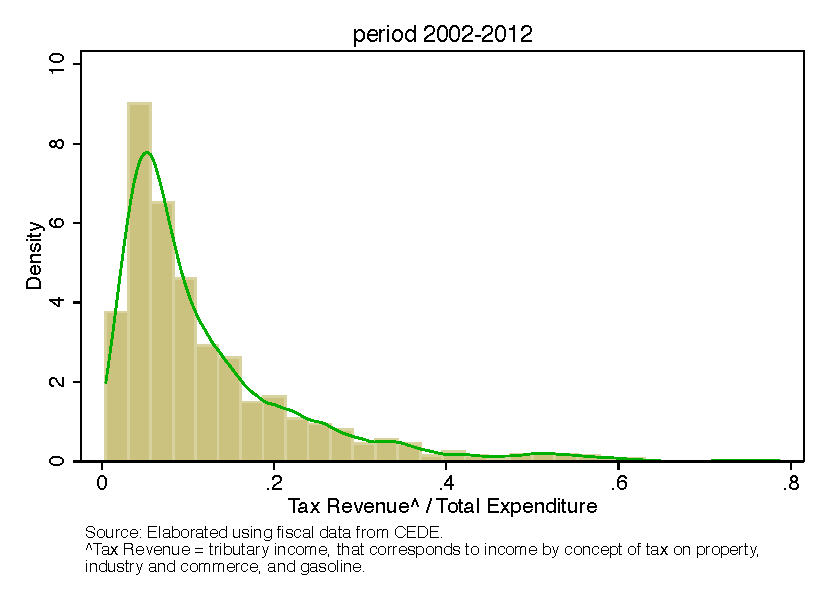
\includegraphics[width=1\textwidth]{Chapter3/Figures/figure1.pdf}
\end{center}
\end{figure}

The variation is not simply a proxy for economic activity, as Figure \ref{chapter3_fig:distributionrevenues} shows. Panel A plots the distribution of different tax revenues per capita at the municipal level, averaged from 2000 to 2012.\footnote{Tax revenues are in constant Colombian pesos from 2008.} Panel B shows the same results normalized using nighttime lights to proxy for economic activity \citep{vernon11}. The first column presents logged tributary income while the second shows the distribution of logged property tax income, which comprises the bulk of local revenue.\footnote{Both are logged given their highly skewed distributions, with a long right tail of municipalities with larger tributary and property tax income.} 

The large variation in tax receipts reflects the freedom that local authorities have in designing tax institutions. While the municipal mayor (the highest local-level executive authority) is in charge of updating the land registry, the city council (the municipal legislative body) issues the municipality's tax statute, which includes the tax rates, the type of properties for which each rate applies, the collection methods, and the payment incentives and fines.\footnote{As stated above, the cadaster is supposed to be updated every five years, but mayors are responsible for initiating the process. Then the national geographic institute, Instituto Geogr\'afico August\'in Codazzi (IGAC), is supposed to carry out the actual update with municipal resources. Although the municipal council sets tax rates, they must fall within a range defined by the National Congress. The current range for property tax is 5-16 per thousand for all types of properties. \citet{nunez05a} reviews Colombia's local tax system.} Property tax rates vary substantially between rural and urban areas, and may or may not vary by type of property or its specific use (e.g. private housing, production, or commercial purposes). In addition, systems can be mixed within municipalities, with some properties and businesses taxed according to one rule (e.g. the value of the property recorded in the municipal cadaster), and others according to another (e.g., the socioeconomic conditions of the neighborhood where the properties are located). The majority of municipalities have mixed systems that combine various schemes.

\begin{figure}[H]
\begin{center}
\caption{Tax revenue across Colombian municipalities, by type}
\label{chapter3_fig:distributionrevenues}
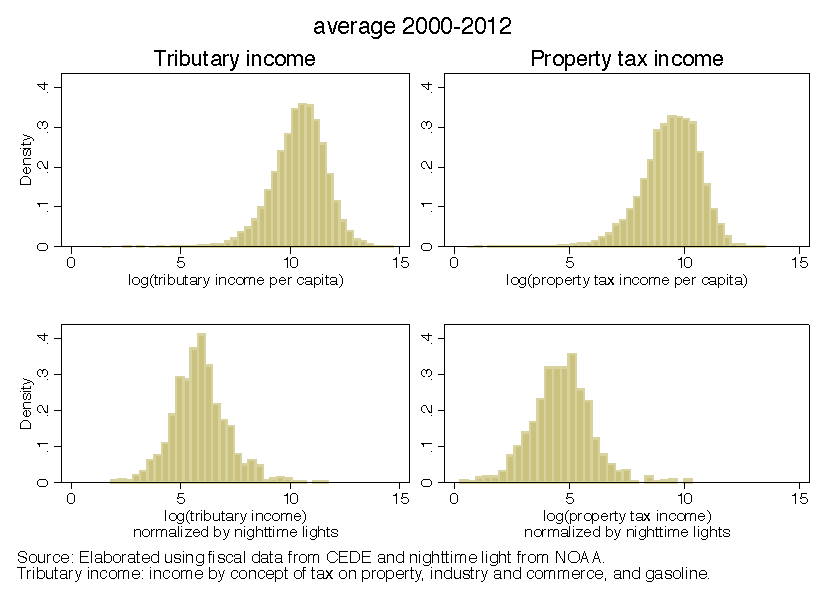
\includegraphics[width=1\textwidth]{Chapter3/Figures/figure2.pdf}
\end{center}
\end{figure}

Regardless of the tax rates and system, the cadaster forms the basis of property taxes.\footnote{Some residents pay property taxes even in the absence of formal title, because it is a way to demonstrate continual presence on a parcel of land. According to Colombian law, investments in land that make it ``socially productive'' can be rewarded with formal property rights for the land in question after five consecutive years of residence (Law 200 of 1936).} The cadaster includes the property values and the physical traits of properties. Outdated cadasters reduce the amount of revenue a municipality collects in property taxes, because recorded property values are lower than the true values \citep{iregui-b.b.04a}. 

\subsection{The capture of local tax and property institutions}

In Latin America, only Brazil and Venezuela have more decentralized systems, and in the rest of the countries in the region, provincial or national governments are in charge of tax legislation. In Colombia, fiscal autonomy was pursued because policymakers thought that it, combined with other decentralization reforms, could help end the war \citep[534, 541]{eaton06a}. The Betancur administration (1982-1986) approved the direct election of mayors that began in 1988, and the two subsequent administrations under Barco and Gaviria devolved fiscal authority and budgetary responsibility to municipalities for several public goods such as education, health, and road upkeep. 

Unfortunately, despite those changes (and partly as a result of them), the civil war intensified and spread in the 1990s \citep{sanchezmar-palau06a, steeleschubiger15a,steele17a}. Municipalities became attractive targets for armed groups because of the transfers and royalties they received and because the state was insufficiently equipped to provide security to them. \citet[537]{eaton06a} writes, ``...the state now funds its own destabilization because armed groups on the left and right have been able to appropriate decentralized public revenues and to use these funds to further reduce the state's already limited monopoly over the use of force.'' The influence of armed groups over locally elected politicians could be substantial.   

In Colombia, insurgents and right-wing paramilitary groups differed in their approaches to capture the state \citep{lopez-hernandez10a, eaton06a, 07a}. Paramilitary groups frequently colluded with state forces, but were independent of them. They forged extensive ties to regional- and national-level politicians \citep[16]{gutierrez-sanin10c}. Indeed, paramilitaries were embraced, and, in some cases, even founded by the country's regional political elites \citep{romero03a, ronderos14a, duncan06a}.  

In contrast, the FARC focused on local organization, particularly through the Juntas de Acci\'{o}n Communal (JACs), committees based in the rural hamlets within municipalities. While the FARC also engaged with some municipal-level and national-level officials, they did so to a far lesser extent then the paramilitaries.\footnote{For example, in 2010 only 10 of the 277 alcaldes and municipal council members under investigation for ties to illegal armed groups were linked to the FARC; similarly, only 4\% of the congress was investigated for ties to the FARC, compared to 35\% to paramilitary groups \citep[33]{lopez-hernandez10a}.} As \citet[18-19]{gutierrez-sanin10c} points out, insurgents are less reliable partners for politicians, because they are anti-state. Consistent with their leftist ideology, insurgents tried to mobilize and work with peasants and workers who were traditionally shut out of the political system.  The distinct ``constituencies'' of insurgents and paramilitaries imply differing preferences over policies.

A particularly fraught policy area that armed groups intervened in is land formalization, which has implications for local tax performance. Right-wing paramilitaries were founded by large landowners and narco-traffickers who began to purchase tracts of land. As they expanded, they displaced peasants and claimed their land \citep{romero00a, ronderos14a, reyes09a}. To legitimate this transfer of land, paramilitaries sought to formalize property through the state. This was consistent with what we noted above: traditionally, elites have been able to secure legal title to their property, while poor peasants face multiple barriers to doing so. Updating cadasters to reflect newly acquired or changed properties (for instance, an enlarged plot of land) is consistent with an interest in securing property rights, even if the property is illegally acquired (for instance through claiming the land of a displaced household).\footnote{\citet{ibanezmunoz11a} find that the concentration of land between 2000 and 2009 increases as the result of an increase in plots and an increased number of plots purchased by few people.} 

Left-wing insurgents favored more equitable land distribution but not private property rights \citep{bernal-morales14a}. One way they promoted this goal was through land invasions, where poor peasants and workers would occupy state lands (\textit{bald\'{i}os}) or private property. However, such invasions were typically not formalized legally. More common in insurgent areas was a preference for excluding or prohibiting representatives of the state from surveying the land or plotting the property -- necessary steps in the formalization process.\footnote{Corporaci\'on Regional para el Desarrollo Sostenible del Area de Manejo Especial la Macarena (CORMACARENA) official interview with the authors, Vista Hermosa, 26 January 2011. This official told us he could not conduct land surveys in the area because the FARC would not permit it.}  

Given the divergent preferences of and incentives for armed groups to shape local property institutions, we expect differences in local property tax performance overall. We propose four hypotheses:

\begin{quotation}
In areas with substantial FARC and ELN violence: 

\noindent $H_{1a}$ Tax revenues per capita will be lower because fewer properties will be formalized.

\noindent $H_{1b}$ Left wing parties will tend to outperform in mayoral and municipal council elections controlling for the pre-existing partisan balance.

\bigskip
In areas with substantial paramilitary violence:

\noindent $H_{2a}$ Tax revenues per capita will be higher because more property will be formalized. 

\noindent $H_{2b}$ Right wing parties will tend to outperform in mayoral and municipal council elections controlling for the pre-existing partisan balance.
\end{quotation}

Though we expect tax revenue to be higher in areas with paramilitary presence, and lower in areas with insurgent presence, we do not argue that right-wing paramilitaries or the elites that supported them favored increased taxation, or that the left-wing insurgents opposed redistribution. Instead, armed groups' preferences over tax rates and enforcement are ambiguous in Colombia. Paramilitaries might try to benefit supporters by pushing for lower rates and lax enforcement of property taxes. This position would be consistent with historical precedent in the 20th century: \citet{sanchez-talanquer18a} finds that following large-scale land reform attempts, local elites registered property in the cadaster to establish their property rights, but manipulated property value to avoid paying higher tax. At the same time, paramilitaries could benefit from an increase in local tax revenue because they issued lucrative contracts to supporters to carry out municipal functions like health services \citep{eaton06a, verdad-abierta15b}.\footnote{Though ideally we could test the effects of armed groups' influence on tax rates and enforcement, we do not have the data to do so. In the end what we do test is the net effect of their influence on local property tax revenue. These data indicate that whatever is happening with tax rates and enforcement, land formalization measures increase tax revenue overall.} New landowners could also calculate that paying taxes was a small cost to pay for securing property, and employ tax resources to expand their control over the local bureaucracy and bargaining power relative to higher levels of government \citep{sanchez-talanquer18a,pardelli2018}. Moreover, short-term development of specific local administrative capacities does not prevent the long-term hollowing out and capture of the state in Colombia \citep{stasavage2014}. 
%[[AS: I cut this segment because it made it difficult for me to follow: "to consolidate their power by pushing wages downward to control labor mobility, while"; also changed "privatization" of the state to "capture."]]

Insurgents, though they did favor redistribution, preferred not to work through the state's institutions because doing so would legitimate the state. The FARC issued its own tax code, targeting the wealthy in areas of their influence (see below). In terms of property rights, the insurgents preferred to impede the efforts of the state \citep{bernal-morales14a} and regulate land on its own.\footnote{One example of the FARC's intransigence on state-backed property rights was its opposition to land restitution for the internally displaced through the Victims Law of 2011, calling it ``legal dispossession'' \citep{bernal-morales14a}.}  

Before we explain how we test our hypotheses, we first summarize temporal trends in capture over the course of the war. 
	
\subsection{Civil war dynamics and capture in Colombia}

The dynamics of the civil war in terms of territorial control and violence have changed significantly over time. We separate the war's recent evolution, and the armed groups' capture strategies, into four periods and organize the statistical analysis around these four periods because pooling them would effectively assume that armed actors had the same ability to influence tax policies in every year, which strikes us as substantively unrealistic. The four periods (described in detail in Appendix H) can be defined as follows: 

\begin{itemize}

\item \textbf{1988-1996: FARC ascendancy}. 
According to one estimate the FARC went from a presence in 173 of the country's municipalities in 1985 to 622 by 1995 \citep[28]{echandia06a}. 
By the end of the period, the FARC and the ELN both enforced election boycotts in areas under their control, and threatened elected mayors and local council members \citep{el-tiempo97a}. 
While some regional politicians supported paramilitaries' formation during this period \citep[37]{ronderos14a}, there is little evidence that paramilitary groups tried to capture political institutions directly at the local level during this period.

\item \textbf{1997-2002: Paramilitary expansion}. 
In 1997, regional paramilitary groups united under the umbrella group United Self-Defense Forces of Colombia (AUC) and the war spread. By 2001, the AUC was powerful enough to convene a meeting with nearly 100 politicians to formulate a concerted effort to win elections at all levels, and to support \'Alvaro Uribe's candidacy for president in 2002 (known as the Santa Fe de Ralito pact). Compared to the paramilitaries, the FARC's influence remained indirect during this period as the group eschewed official electoral politics during this period, preferring to threaten municipal candidates that the group did not approve of, or acting mayors.

\item \textbf{2003-2006: Paramilitary demobilization}.
In 2003, the Uribe administration negotiated a ceasefire with paramilitary groups and eventually adopted the `Justice and Peace' law, allowing paramilitary commanders to demobilize their troops in exchange for lenient sentences. Paramilitary demobilizations from 2003 to 2005 transformed the war into a contest between the state and remaining insurgent groups (the FARC and ELN). The conflict with the FARC continued apace during this period, with no change in their capture strategy.

\item \textbf{2007-2010: State resurgence}.
Having pushed the FARC into peripheral areas by the end of 2006, the Colombian military and police redeployed to major population centers and roads, improving measures of security. The weakened FARC agreed to peace talks following the 2010 election of Uribe's Minister of Defense, Juan Manuel Santos. Former paramilitary groups morphed into new organizations---including the ``Black Eagles,'' and drug-trafficking groups such as the ``Urabe\~{n}os'' and the ``Rastrojos'' — which sometimes engaged in actions against the FARC, the ELN, and the civilian population, though at much lower rates than in previous times.

\end{itemize}

Taking into account these time periods, Figure \ref{chapter3_fig:violence_revenues} shows the department-level relationship between cumulative attacks by armed group and average property tax revenues in the following time period.\footnote{There are 32 departments in Colombia. This administration level is equivalent to US states.} There are two main takeaways: first, departments in Colombia vary widely in the correlation between tax performance and the type and level of armed group presence; second, and following the historical shifts of the Colombian war, this variation changes over time, a feature that will be exploited in the empirical specification to test our hypotheses, and in the substantive interpretation of results.\footnote{Correlations are carried out at the department level since municipalities are the lowest administrative unit in our data.}

\medskip


\begin{figure}[H]
\begin{center}
\caption{Relationship between property tax revenues and attacks per armed group and time period across Colombian departments}
\label{chapter3_fig:violence_revenues}
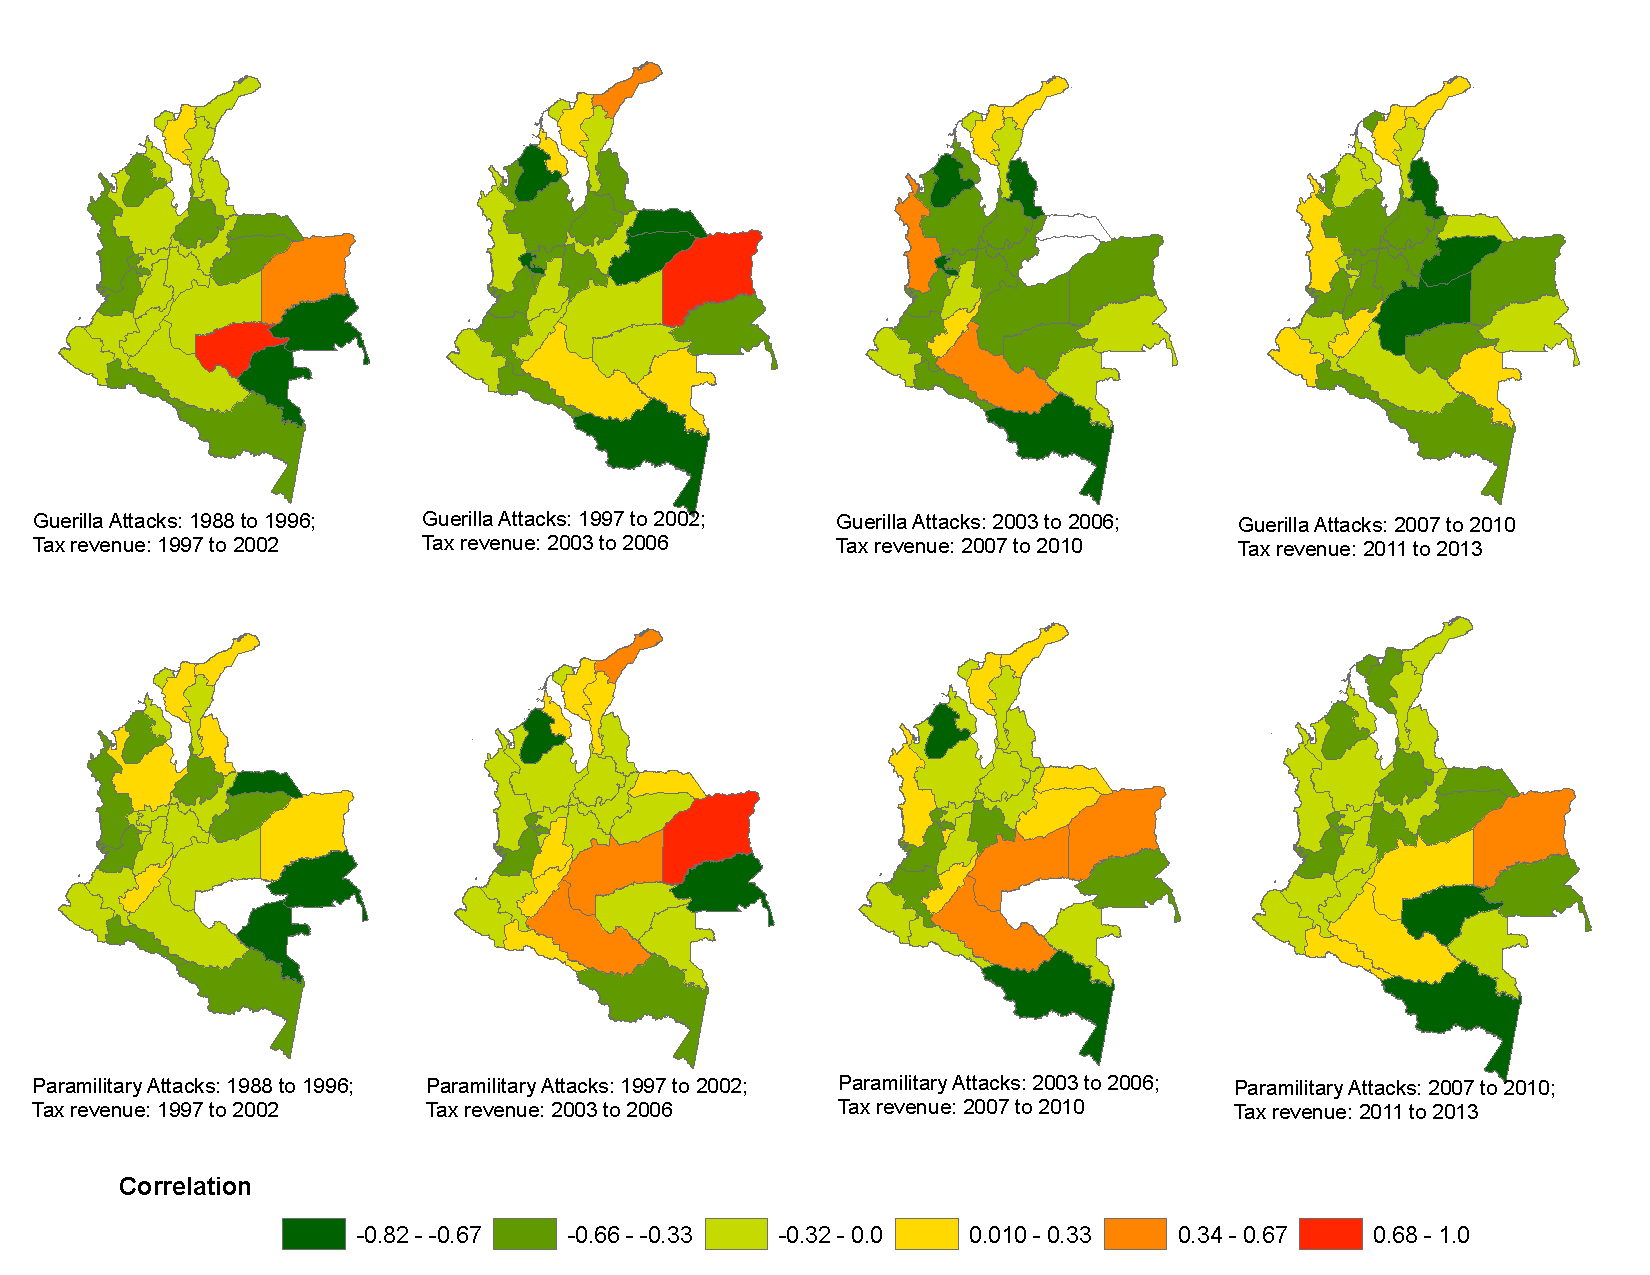
\includegraphics[width=1\textwidth]{Chapter3/Figures/figure3.pdf}
\end{center}
\end{figure}
Notes: Violence data from the Human Rights Observatory of the Office of the Vice-President, Colombia, and fiscal data from CEDE. Revenues are average property tax receipts by specified time period. Attacks are cumulative attacks per 100,000 inhabitants per armed group, by specified time period. 

\subsection{Data}

Table \ref{chapter3_tab:descriptive} provides descriptive statistics of our main outcome variables, used to test both the main empirical relationships and the mechanisms described in our testable hypotheses (Panel A). Outcomes include logged tax revenues per capita, proxies of cadastral performance, the land informality rate and electoral outcomes. Tax revenues are highly skewed, with a long right tail of municipalities with substantially greater tax revenues per capita than others.\footnote{The wealthiest municipalities had tax receipts as much as ten standard deviations above the mean.} We therefore run our estimation of the impact of violence on property tax revenues per capita on logged values.\footnote{The results are substantially the same when we add to the set of controls the log of the municipal population instead of using per capita tax revenue.}

Table \ref{chapter3_tab:descriptive} also describes the independent variables of interest (Panel B), namely the cumulative attacks perpetrated by each of the two main armed groups, during each one of the four periods that mark the evolution of Colombia's civil war, as described in the ``Civil War Dynamics and Capture in Colombia'' section.\footnote{See the Appendix \ref{data_appendix3} for detailed descriptions of all the variables and measures.} Measuring the influence exercised by an armed group over a specific location is extremely challenging. Indicators of presence and non-violent coercion over a large set of municipalities cannot be systematically recorded in an objective way. Violence, on the other hand, while more easily observed, is only imperfectly correlated with territorial dominance. For instance, it may be the case that municipalities with low levels of violence or no armed contestation represent an armed group stronghold, where tax policies are likely to be influenced.

%%-----------------------------------------------------------%

% Table 1 Descriptive Stats

\begin{table}[h]
\centering 
\caption{Descriptive statistics of main variables}
\label{chapter3_tab:descriptive}
\scalebox{0.65}{
\begin{tabular}{l c c c c c}\hline\hline
\multicolumn{1}{c}{\textbf{Variable}} & \textbf{Mean}
 & \textbf{Std. Dev.}& \textbf{Min.} &  \textbf{Max.} & \textbf{N}\\ \hline
 \\
 \multicolumn{6}{c}{Panel A. Outcomes} \\

{\it Tax revenues per capita}	&		&		&		&		&		\\ 

Log property tax revenues per capita 1997-2002&        2.32&        1.08&           0&           6&        1108\\
Log property tax revenues per capita 2003-2006&        2.70&        1.00&           0&           6&        1107\\
Log property tax revenues per capita 2007-2010&        2.82&        1.06&           0&           6&        1111\\
Log property tax revenues per capita 2011-2013&        2.94&        1.11&           0&           7&        1111\\




\\
{\it Cadastral performance}	&		&		&		&		&		\\ 

Per capita land value 2003-2006&        4.60&        5.79&           0&          79&         974\\
Cadastral update lag 2003-2006&        6.82&        3.87&           0&          50&         892\\
Num. cadastral updates 2003-2006&        1.49&        0.67&           0&           4&         979\\



\\
{\it Land ownership}	&		&		&		&		&		\\ 

Land informality rate 2003-2006&        0.20&        0.23&           0&           1&         954\\

\\
{\it Electoral outcomes}	&		&		&		&		&		\\ 

Uribe + Conservative party coalition 1997 Mayor election&        0.28&        0.45&           0&           1&         986\\
Uribe + Conservative party coalition 2000 Mayor election&        0.26&        0.44&           0&           1&         955\\
Uribe + Conservative party coalition 1997 and 2000 Mayor elections&        0.32&        0.46&           0&           1&        1182\\
Uribe + Conservative party coalition 2003 Mayor election&        0.23&        0.42&           0&           1&         908\\
Uribe + Conservative party coalition 2007 Mayor election&        0.60&        0.49&           0&           1&        1106\\
Uribe + Conservative party coalition 2003 and 2007 Mayor elections&        0.61&        0.49&           0&           1&        1182\\
Uribe + Conservative party coalition 2011 Mayor election&        0.43&        0.50&           0&           1&        1040\\


\\
 \multicolumn{6}{c}{Panel B. Violence} \\

Log guerrilla attacks per capita, 1988-1996&      -35.42&       31.30&        -115&           0&        1182\\
Log paramilitary attacks per capita, 1988-1996&      -35.87&       31.53&        -105&           0&        1182\\
Log guerrilla attacks per capita, 1997-2002&      -29.38&       19.80&         -82&           0&        1182\\
Log paramilitary attacks per capita, 1997-2002&      -30.02&       20.04&         -74&           0&        1182\\
Log guerrilla attacks per capita, 2003-2006&      -18.12&       12.67&         -53&           0&        1182\\
Log paramilitary attacks per capita, 2003-2006&      -19.61&       14.10&         -53&           0&        1182\\
Log guerrilla attacks per capita, 2007-2010&      -13.94&       13.07&         -48&           0&        1182\\
Log paramilitary attacks per capita, 2007-2010&      -16.49&       15.73&         -55&           0&        1182\\
Log guerrilla attacks per capita, 2003-2010&      -32.06&       23.73&        -101&           0&        1182\\
Log paramilitary attacks per capita, 2003-2010&      -36.10&       27.71&        -108&           0&        1182\\



\hline \hline
\multicolumn{6}{p{1.4\textwidth}}{\footnotesize{Notes: All data sources are described in Appendix \ref{data_appendix3}.}} \\
\end{tabular}
}
\end{table}

However, non-violent dominance is unlikely to occur without any violence inflicted in the past, either as a way to legitimize influence with the citizenry or to oust any contesting (legal or illegal) group. It is thus reasonable to assume that the ability to inflict localized violence over a relatively long period could be expected to translate into influence in different ways. Moreover, as all our results are robust to controlling for violence by the other actor, we posit that municipalities with greater violence are more likely to be captured by the perpetrating armed group.\footnote{A more stringent test is to focus on the subsample of places where violence by both groups is recorded, dropping the municipalities where one group does not engage in any violence at all during the sample period. Even with the statistical power reduction implied by the limited sample, Appendix D shows that out main results are robust to this exclusion.}

We thus follow a growing empirical literature on the Colombian conflict (see e.g. \citet{acemoglurobinson13a}, \citet{fergussonetal2016} and \citet{fergussonetal2018}) and use a past stock measure of violence over a period of years as an (imperfect) indicator of influence. \citet{arjonaotalora11a} compare existing databases of civil war violence in Colombia to survey evidence on armed groups' presence (for the small subsample of municipalities for which the latter is available) and conclude that while violence is likely to {\it underestimate} --by roughly the same magnitude- both guerrilla and paramilitary control, there is a non-negligible correlation between both measures.\footnote{The authors do not use cumulative past violence, hence the correlation of survey-based presence indicators with our proposed measure is probably larger.} 

To further validate our proposed measure of armed groups' influence, we report the correlations between groups' cumulative attacks and other (group-specific) proxies of presence. The recent peace agreement signed by the Colombian government and FARC in September 2016 was followed by the demobilization of over 10,000 FARC combatants in the so called {\it Espacios Territoriales de Capacitaci\'on y Reincorporaci\'on}, ETCR (Spanish for territorial areas of training and reincorporation). The ETCR are located in 25 of the municipalities of FARC's highest historical influence. The correlation between an ETCR indicator and cumulative guerrilla attacks of the last conflict period we study (2007 - 2010) is 0.3 (significant at the 1\% level). Instead, the correlation of ETCR with cumulative paramilitary attacks is 0.09. Similarly, following a DDR process with the government of \'{A}lvaro Uribe (see ``Civil War and Capture in Colombia'' section, several paramilitary units adding up to over 35,000 ex-combatants) demobilized in 36 municipalities where, arguably, their dominance was high. The correlation between an indicator of these municipalities and cumulative paramilitary attacks over the period 1997 - 2002 is 0.1, and significant at the 1\% level. Instead, the correlation with cumulative guerrilla attacks is 0.02, and not significant.\footnote{For all the above reasons, we believe that violence is an imperfect but valid proxy of armed influence. But even if it was not, the strong relationship of violence to changes in local fiscal institutions that we document in this paper is an important fact that has not been previously documented, and that should inform our thinking on how conflict influences state building and development.}

Similar to the case of tax revenues, attacks by guerrilla fronts and paramilitary blocks are highly skewed, especially in the 1988-2010 period (see also Figure \ref{chapter3_fig:map}). The most violent municipalities had attacks over eight standard deviations above the mean. We thus normalize attacks by population so as to capture violence intensity, and use logged values in the regressions (since normalized variables remain highly skewed).\footnote{The statistical significance of the results below becomes weaker when using a log-linear model with unlogged violence per-capita, with t-statistics in the 1.3-1.6 range, though all results retain the same sign. This means that the results are surely not driven by outliers in attacks, as logging the per capita attack variable effectively attenuates those observations' influence on the estimates.}

\begin{figure}[H]
\begin{center}
\caption{Guerrilla and paramilitary attacks across Colombian municipalities}
\label{chapter3_fig:map}
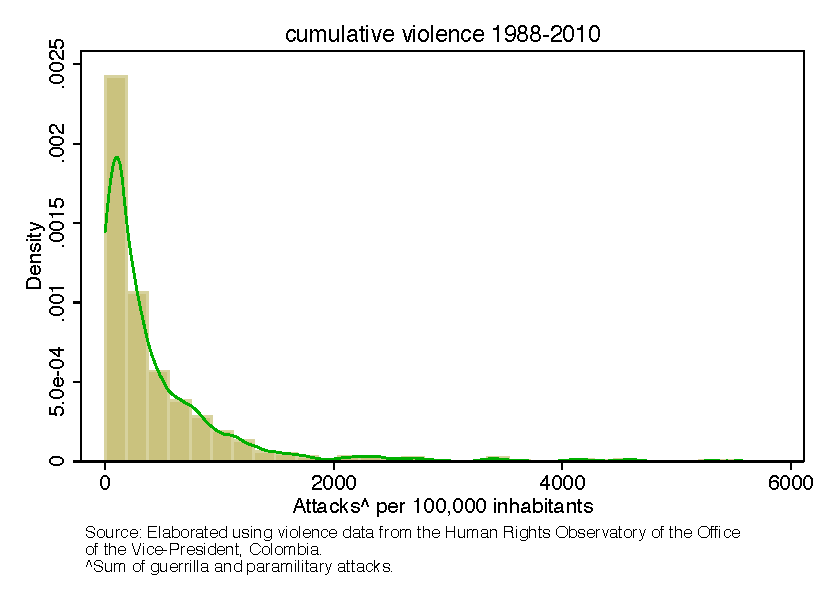
\includegraphics[width=1\textwidth]{Chapter3/Figures/figure4.pdf}
\end{center}
\end{figure}

Appendix \ref{data_appendix3} provides a detailed description of both the main and all the additional variables (summarized in Table \ref{appendix3:description_vars}). All of our specifications control for a large set of municipal-level potential confounders, including natural resource royalties and transfer payments, vote share by political party for mayors' elections, the location of military bases, a dummy of `peaceful' municipalities (those without attacks during our entire sample period), the number of people displaced due to the armed conflict, coca production and municipal geographic characteristics. We also control for a resources-endowment additive index, that includes the production of gold, silver, platinum, nickel and iron.\footnote{Note that some of these variables are potentially {\it bad controls} as they can respond to cumulative past violence. In the ``Additional Robustness Checks'' subsection we discuss this issue and show that our results are not affected by post-treatment bias.} 


\subsection{Estimation} 

Because the modern internal conflict in Colombia had four distinguishable periods with their own intensity and dynamics, as summarized in the subsection on ``Civil War Dynamics and Capture in Colombia'', we test how violence-related capture during each specific period correlates with local tax performance during the subsequent period. We examine lagged outcomes both because tax institutions cannot shift overnight and because studying the relationship between conflict events within a given period and tax institutions immediately after that period minimizes simultaneity problems. 

Running a standard panel data approach with municipality and time fixed-effects would entail two untenable assumptions: (1) that the conditional impact of violence on taxes operates in the short term; and (2) the treatment effect of influence (as proxied by violent incidents) is the same in every period. Both seem substantively problematic. On (1), tax institutions are slow to change, in part because mayors and council member have a 3 or 4 year office period (depending on if before or after 2003) and they update the cadaster and the rates once in that period, if anything. On (2), the intensity of violence varied significantly across periods, so fitting a model that assumes constant marginal effects of violence on outcomes would be incorrect. 

We therefore estimate an OLS specification at the municipality level separately for each of the periods mentioned above. With tax revenue, for example, we estimate:

		\begin{align}
			\label{eq:revenue}
			\mbox{Tax Revenue}_{i,t} = \alpha + \gamma_d+  \beta_1 \mbox{Cum. Guerrilla Attacks}_{i,(t-\Delta \text{ to } t-1)} \nonumber \\ 
			+ \beta_2 \mbox{Cum. Paramilitary Attacks}_{i,(t-\Delta \text{ to } t-1)} + \Phi \mathbf{X}_{i,t} + \epsilon_{i,t} \\ \forall \ t \in \{(1997 \text{ to } 2002), (2003 \text { to } 2006), (2007 \text { to } 2010), (2011 \text{ to } 2013) \nonumber \}
		\end{align}
\noindent where 	 	
 $\mbox{Tax Revenue}_{i,t}$ is the log property tax revenue per capita in a municipality, $i$, in a given period, $t$, after each of the described violence periods;\footnote{We report multiple post-treatment years to explore potential cumulative effects.} $ \mbox{Cum. Guerrilla Attacks}_{i,(t-\Delta \text{ to } t-1)}$ and $\mbox{Cum. Paramilitary Attacks}_{i,(t-\Delta \text{ to } t-1)}$ capture logged total attacks per capita that accumulate over each period described in the subsection ``Civil War Dynamics and Capture in Colombia'' subsection, and preceding $t$; $\mathbf{X}_{i,t}$ is a vector of municipality-level control variables as described in the previous subsection.\footnote{Municipal-level production of coca is available only since 1999. Our post 1999 results are robust to adding this variable in the vector $\mathbf{X}_{i,t}$. We address potential concerns regarding the inclusion of post-treatment controls explicitly below.} We also include a Department fixed-effect, $\gamma_d$, to account for any department-level time-invariant heterogeneity across each of the 32 second-level administrative units, the next level administrative unit up from the municipality. 
We are thus working off within-department variation in violence, controlling for a range of geographic factors. Hence, our estimates account for the {\it excess} tax revenue in municipalities that experience more violence by one party or the other above the department mean. We report robust standard errors throughout, clustered at the department level.\footnote{We believe this to be a conservative approach. If we follow \citet{acemoglurobinson13a} by simply using robust standard errors all results become somewhat stronger statistically.}

Our identifying assumption with this approach is that levels of violence during each period of the internal conflict were conditionally independent of future tax revenues. Our controls are grounded in the rich literature on civil war, which cites incentives for capture and the advantages (or disadvantages) of terrain as key determinants of contestation. One concern with this approach is that we could simply be picking up enduring cross-sectional within-department differences, correlated both with the presence of different armed groups as well as with the trajectory of tax revenues. To rule this out we include a set of regressions controlling for tax revenue in the municipality at the end of the period prior to each period in which cumulative violence is measured ($\mbox{Tax Revenue}_{i,t-\Delta-1}$ in the notation above). When estimating the partial correlation of tax revenue from 2003-6 with violence from 1997-2002, for example, we include a specification controlling for tax revenues in 1993-1996, and so forth with the other time periods.

\section{Results}

\subsection{Violence and tax revenue}

As a first glance at armed groups' influence on tax institutions, we use specification (1) to estimate the relationship between cumulative past violent activity by armed groups and property tax revenue. As shown in Table \ref{chapter3_tab:main}, we find that violence perpetrated by guerrillas is consistently negatively associated with property tax revenue, while violence by paramilitaries is positively correlated with it. 

Table \ref{chapter3_tab:main} focuses on four different time periods. Columns 1 and 2 show the relationship between logged total violence per capita from 1988-1996 on average logged tax revenues per capita in 1997 through 2002. Columns 3 and 4 show the relationship between violence in 1997-2002 and tax revenues in 2003 through 2006. Columns 5 and 6 show the relationship between violence in 2003-2006 and tax revenues in 2007 through 2010. Lastly, columns 7 and 8 show the relationship between violence in 2007-2010 and tax revenues from 2011 to 2013, the last period we have data for. 

%%-----------------------------------------------------------%
%

% Table 2. Main Table
\newpage

%\begin{landscape}
\begin{table}[htbp]\def\sym#1{\ifmmode^{#1}\else\(^{#1}\)\fi}
\caption{Cumulative violence and property tax performance}
\label{chapter3_tab:main}
\begin{center}
\scalebox{0.65}{
\begin{tabular}{lcccccccc}

\hline \hline 
\multicolumn{9}{l}{Dependent variable: {\it Log of property tax revenue per capita} over period:}\\


&\multicolumn{2}{c}{1997-2002}              &\multicolumn{2}{c}{2003-2006}              &\multicolumn{2}{c}{2007-2010}              &\multicolumn{2}{c}{2011-2013}              \\\cmidrule(lr){2-3}\cmidrule(lr){4-5}\cmidrule(lr){6-7}\cmidrule(lr){8-9}
            &\multicolumn{1}{c}{(1)}         &\multicolumn{1}{c}{(2)}         &\multicolumn{1}{c}{(3)}         &\multicolumn{1}{c}{(4)}         &\multicolumn{1}{c}{(5)}         &\multicolumn{1}{c}{(6)}         &\multicolumn{1}{c}{(7)}         &\multicolumn{1}{c}{(8)}         \\
\addlinespace
\begin{tabular}[c]{@{}l@{}}Log guerrilla attacks\\ per capita \underline{1988-1996}\end{tabular}&     -0.0746\sym{***}&     -0.0384\sym{***}&                     &                     &                     &                     &                     &                     \\
            &    (0.0087)         &    (0.0073)         &                     &                     &                     &                     &                     &                     \\
\addlinespace
\begin{tabular}[c]{@{}l@{}}Log paramilitary attacks\\ per capita \underline{1988-1996}\end{tabular}&      0.0715\sym{***}&      0.0367\sym{***}&                     &                     &                     &                     &                     &                     \\
            &    (0.0089)         &    (0.0072)         &                     &                     &                     &                     &                     &                     \\
\addlinespace
\begin{tabular}[c]{@{}l@{}}Log guerrilla attacks\\ per capita \underline{1997-2002}\end{tabular}&                     &                     &     -0.0951\sym{***}&     -0.0318\sym{**} &                     &                     &                     &                     \\
            &                     &                     &    (0.0090)         &    (0.0100)         &                     &                     &                     &                     \\
\addlinespace
\begin{tabular}[c]{@{}l@{}}Log paramilitary attacks\\ per capita \underline{1997-2002}\end{tabular}&                     &                     &      0.0903\sym{***}&      0.0302\sym{**} &                     &                     &                     &                     \\
            &                     &                     &    (0.0095)         &    (0.0104)         &                     &                     &                     &                     \\
\addlinespace
\begin{tabular}[c]{@{}l@{}}Log guerrilla attacks\\ per capita \underline{2003-2006}\end{tabular}&                     &                     &                     &                     &     -0.0708\sym{***}&     -0.0173\sym{*}  &                     &                     \\
            &                     &                     &                     &                     &    (0.0130)         &    (0.0082)         &                     &                     \\
\addlinespace
\begin{tabular}[c]{@{}l@{}}Log paramilitary attacks\\ per capita \underline{2003-2006}\end{tabular}&                     &                     &                     &                     &      0.0643\sym{***}&      0.0137\sym{+}  &                     &                     \\
            &                     &                     &                     &                     &    (0.0123)         &    (0.0077)         &                     &                     \\
\addlinespace
\begin{tabular}[c]{@{}l@{}}Log guerrilla attacks\\ per capita \underline{2007-2010}\end{tabular}&                     &                     &                     &                     &                     &                     &     -0.0655\sym{*}  &     -0.0120         \\
            &                     &                     &                     &                     &                     &                     &    (0.0248)         &    (0.0074)         \\
\addlinespace
\begin{tabular}[c]{@{}l@{}}Log paramilitary attacks\\ per capita \underline{2007-2010}\end{tabular}&                     &                     &                     &                     &                     &                     &      0.0472\sym{*}  &      0.0078         \\
            &                     &                     &                     &                     &                     &                     &    (0.0219)         &    (0.0067)         \\
\addlinespace
Observations&         986         &         986         &        1070         &        1070         &        1107         &        1107         &        1107         &        1107         \\
R-squared   &       0.533         &       0.672         &       0.565         &       0.754         &       0.542         &       0.818         &       0.531         &       0.874         \\
Controls$^a$&  \checkmark         &  \checkmark         &  \checkmark         &  \checkmark         &  \checkmark         &  \checkmark         &  \checkmark         &  \checkmark         \\
Depto. FE   &  \checkmark         &  \checkmark         &  \checkmark         &  \checkmark         &  \checkmark         &  \checkmark         &  \checkmark         &  \checkmark         \\
Pre-period tax revenue$^b$&                     &  \checkmark         &                     &  \checkmark         &                     &  \checkmark         &                     &  \checkmark         \\



\hline \hline
\multicolumn{9}{p{1.35\textwidth}}{\footnotesize{Notes: Standard errors in parentheses are clustered at the department level; Significance-level: $^{***}$ 0.1\%; $^{**}$ 1\%; $^*$ 5\%; and $^{+}$ 10\%, refers to two-sided t-tests. Outcome measured in constant 2008 Colombian pesos.
$^a$ Controls include: royalties and transfers per capita, municipality area, elevation, distance to the department's capital, vote share by political party ideology, dummy variable on whether the municipality had no registered homicides in the same period as the attacks  (independent variables), the number of military bases, the number of people displaced, driven out and received by municipality due to conflict, average coca production, and an additive endowment index on the production of gold, silver, platinum, nickel, emeralds and iron.%
$^b$ Estimations include the pre-period property tax revenue per capita, i.e. the period from 1985 to 1987 in column (2), from 1993 to 1996 in (4), from 2000 to 2002 in (6), and from 2003 to 2006 in (8), to pick up part of the enduring cross-sectional within-department differences. }} \\
\end{tabular}
}
\end{center}
\end{table}
%\end{landscape}

Odd columns show that guerrilla attacks are negatively correlated with tax revenues, a relationship that is statistically significant across the four periods. In contrast, cumulative past paramilitary attacks are positively correlated with tax revenues in every period. Even columns show that the results for the first three conflict periods are robust to controlling for pre-period tax revenues. Statistical significance is however attenuated in the last period. This is consistent with the observation that paramilitary groups officially demobilized from 2003 to 2006 (largely becoming criminal bands), and guerrilla groups were weakened from 2007 to 2010 (see section on ``Civil War Dynamics and Capture in Colombia''). Thus, we would not expect the effects to be as strong in the third and especially the fourth period. This effectively turns the last period into a {\it placebo}.\footnote{Figure \ref{chapter3_fig:figure5} is the graphical counterpart of Table \ref{chapter3_tab:main} (even columns). We plot the point estimates as well as the 95\% confidence intervals, documenting that the estimated effects decrease overtime. The differences across conflict periods are not statistically significant, with the exception of the comparison between the first and the fourth period. Again, as expected, during the state resurgence period, point estimates lean towards zero.} 

\begin{figure}[H]
\begin{center}
\caption{Estimated relationship between property tax revenues and attacks per armed group and time period across Colombian municipalities}
\label{chapter3_fig:figure5}

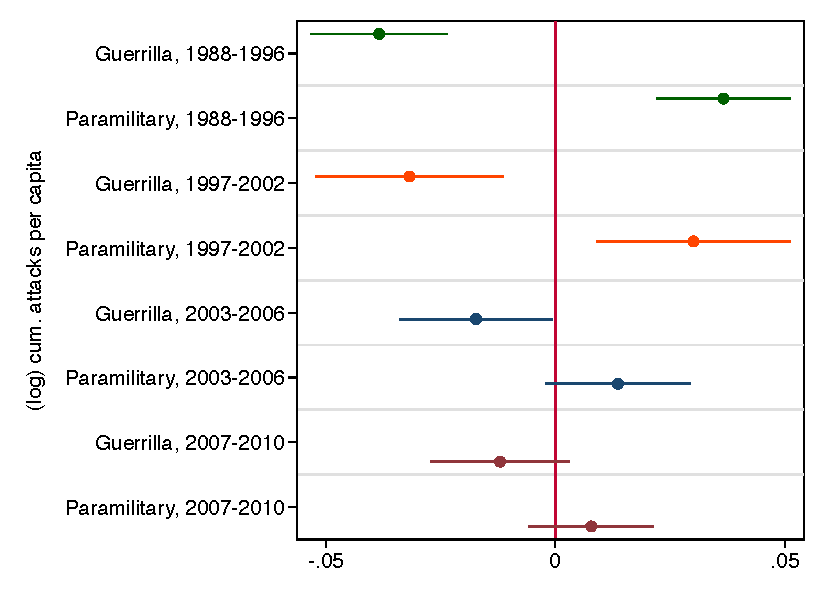
\includegraphics[width=1\textwidth]{Chapter3/Figures/figure5.pdf}
\end{center}
\end{figure}
Notes: Regression estimates from Table \ref{chapter3_tab:main}, columns (2), (4), (6), and (8), respectively. Treatment variables in logs as specified in Table \ref{chapter3_tab:main}.  


Because of the log-log specification, estimated coefficients should be interpreted as the elasticity of per capita property tax revenue with respect to cumulative past violence. Given the estimated elasticities we can compute substantive effects by multiplying them with changes of interest in the independent variable (expressed in terms of percent changes). Using the most demanding specification in column 2 of Table \ref{chapter3_tab:main}, an increase in cumulative per capita guerrilla attacks (paramilitary attacks) over the period 1988-1996 from the median to the 90$^{th}$ percentile of the distribution is associated with an average 37\% drop (13\% increase) in per capita property tax income over the period 1997-2002. An equivalent increase in cumulative violence in the period 1997-2002 is associated with a 16\% drop, and a 11\% increase, in per capita property tax income over the period 2003-2006 for the case of guerrilla and paramilitary attacks, respectively (column 4). Further,  
An equivalent increase in cumulative violence in the period 2003-2006 is associated with a 20\% drop, and a 8\% increase, in per capita property tax income over the period 2007-2010 for the case of guerrilla and paramilitary attacks, respectively (column 6).\footnote{Figure \ref{chapter3_fig:margins} reports the marginal-effect plots of the effect of cumulative past guerrilla and paramilitary violence on property tax revenues, with a horizontal axis support ranging from the median to the 90$^{th}$ percentile.}

\begin{figure}[H]
\begin{center}
\caption{Cumulative violence (1997-2002), tax revenues, and potential mechanisms (2003-2006): change in predictions from the median to the 90$^{th}$ percentile}
\label{chapter3_fig:margins}
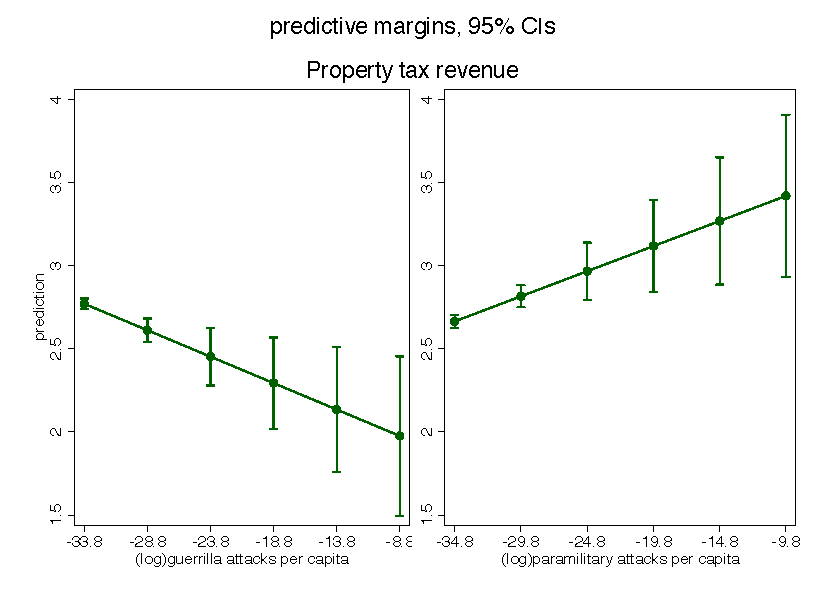
\includegraphics[width=.75\textwidth]{Chapter3/Figures/figure6_part1.pdf}
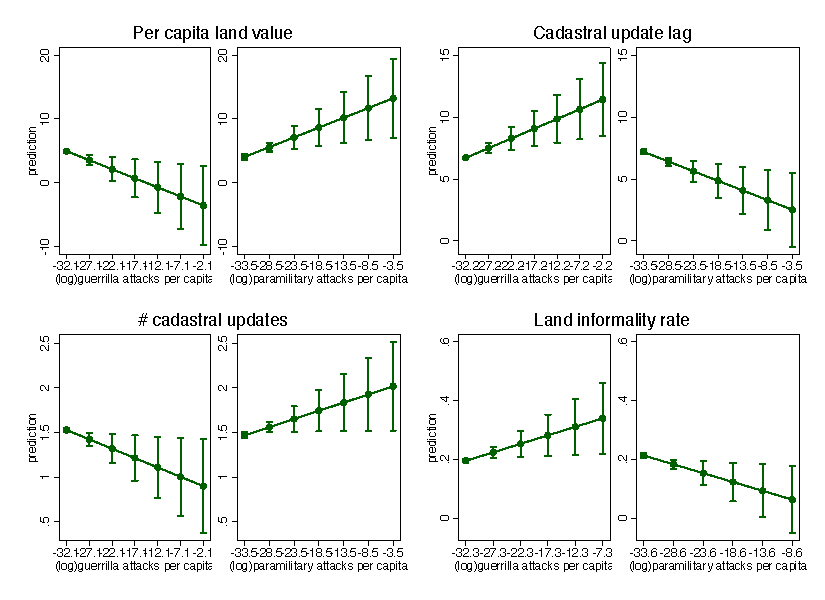
\includegraphics[width=1\textwidth]{Chapter3/Figures/figure6_part2.pdf}
\end{center}
Note: Elaborated using Table \ref{chapter3_tab:main}, second period, and \ref{chapter3_tab:table3} estimates.
\end{figure}

\subsection{Robustness}

While our four conflict periods are based on our substantive theoretical and historical understanding of the evolution of the Colombian civil war, a potential concern is that the results reported in Table \ref{chapter3_tab:main} are just an artifact of an arbitrary aggregation of annual data into these periods. Appendix E shows that this is not the case. We re-run our most demanding empirical specification (including pre-period tax revenues) using year-by-year moving windows in which six (eight) years of cumulative conflict are correlated with three (five)-year aggregations of tax revenues.

Figures \ref{appendix3:moving_window_6years} and \ref{appendix3:moving_window_8years} report the results graphically, respectively for the six and the eight-year moving windows. In both cases, we corroborate the asymmetric correlation of guerrilla and paramilitary cumulative past violence of municipal tax performance. Also consistent with our main results (Table \ref{chapter3_tab:main}) and with the historical account of the conflict (section ``Civil War Dynamics and Capture in Colombia''), Figures \ref{appendix3:moving_window_6years} and \ref{appendix3:moving_window_8years} suggest that armed groups' influence decreases in the later periods, especially for the case of paramilitaries.

\subsection{Implications}
Appendix \ref{appendix3:why_matters} analyzes the implications of the influence that armed groups exert on tax revenues, both for a set of education outcomes that respond to municipal-specific investments and for a proxy of municipal-specific economic performance. Tables \ref{appendix3:consequences_violence} and \ref{appendix3:consequences_economic} suggest that cumulative past guerrilla violence is associated with less human capital accumulation and poor economic performance, respectively. The opposite is true for paramilitary activity.

\subsection{Mechanisms: Tax Institutions and Land Formalization}

What explains the association between violence and tax performance, and particularly the heterogeneity across different armed groups? We expect that a key channel is through land formalization.
 
Recall that the mayor is in charge of managing and updating the land registry, and the city council can decide tax rates, tax collection mechanisms, enforcement, and fines. Since either or both these government levels can be captured by violent groups with vested interests, we explore two things: first, the extent to which the intensity of the internal conflict is correlated with variation in outcomes associated with the responsibilities of both the local authorities related to land formalization and taxation; and second, the extent to which armed groups captured local authorities through electoral outcomes.

Table \ref{chapter3_tab:table3} uses the empirical specification in \eqref{eq:revenue} to estimate the effect of cumulative past guerrilla and paramilitary violence on potential mechanisms related to the functioning of municipal tax institutions and land formalization. In particular, we look at land value (columns 1 and 2), the time elapsed since the last cadastral update (columns 3 and 4), the number of cadastral updates carried out by a municipality (columns 5 and 6) and the share of properties that lack land titles (columns 7 and 8). 

%---------------------------------------
% Table 3. Mechanisms

%\begin{landscape} 
\begin{table}[htbp]
\def\sym#1{\ifmmode^{#1}\else\(^{#1}\)\fi}\caption{Mechanisms: Cumulative violence (1997-2002) and potential mechanisms (2003-2006)}
\label{chapter3_tab:table3}
\begin{center}
\scalebox{0.65}{
\begin{tabular}{lcccccccc}
\hline \hline 
  & (1) & (2) & (3) & (4) & (5) & (6) & (7) & (8)   \\
 \hline 
 \\  

&\multicolumn{2}{c}{\emph{Per capita land value}}&\multicolumn{2}{c}{\emph{Cadastral update lag}}&\multicolumn{2}{c}{\emph{\# cadastral updates}}&\multicolumn{2}{c}{\emph{Land informality rate}}\\\cmidrule(lr){2-3}\cmidrule(lr){4-5}\cmidrule(lr){6-7}\cmidrule(lr){8-9}
\addlinespace
\begin{tabular}[c]{@{}l@{}}Log guerrilla attacks\\ per capita \underline{1997-2002}\end{tabular}&     -0.5266\sym{***}&     -0.2841\sym{*}  &      0.1988\sym{***}&      0.1568\sym{**} &     -0.0315\sym{**} &     -0.0210\sym{*}  &      0.0139\sym{***}&      0.0058\sym{*}  \\
            &    (0.1414)         &    (0.1045)         &    (0.0435)         &    (0.0496)         &    (0.0089)         &    (0.0090)         &    (0.0026)         &    (0.0025)         \\
\addlinespace
\begin{tabular}[c]{@{}l@{}}Log paramilitary attacks\\ per capita \underline{1997-2002}\end{tabular}&      0.5386\sym{***}&      0.3064\sym{**} &     -0.1967\sym{***}&     -0.1557\sym{**} &      0.0284\sym{**} &      0.0183\sym{*}  &     -0.0137\sym{***}&     -0.0060\sym{*}  \\
            &    (0.1455)         &    (0.1077)         &    (0.0456)         &    (0.0515)         &    (0.0084)         &    (0.0087)         &    (0.0025)         &    (0.0024)         \\
\addlinespace
Observations&         939         &         939         &         867         &         867         &         942         &         942         &         927         &         927         \\
R-squared   &       0.361         &       0.445         &       0.293         &       0.298         &       0.450         &       0.462         &       0.515         &       0.574         \\
Controls$^a$&  \checkmark         &  \checkmark         &  \checkmark         &  \checkmark         &  \checkmark         &  \checkmark         &  \checkmark         &  \checkmark         \\
Depto. FE   &  \checkmark         &  \checkmark         &  \checkmark         &  \checkmark         &  \checkmark         &  \checkmark         &  \checkmark         &  \checkmark         \\
Pre-period tax revenue$^b$&                     &  \checkmark         &                     &  \checkmark         &                     &  \checkmark         &                     &  \checkmark         \\


\hline \hline
\multicolumn{9}{p{1.3\textwidth}}{\footnotesize{Notes: Standard errors in parentheses are clustered at the department level; Significance-level: $^{***}$ 0.1\%; $^{**}$ 1\%; $^*$ 5\%; and $^{+}$ 10\%, refers to two-sided t-tests. $^a$ Controls as in Table \ref{chapter3_tab:main}.
$^b$ Due to the lack of 1993-1996 data for these dependent variables, regressions include pre-period property tax revenue per capita from 1993 to 1996 in (2), (4), (6), and (8) to pick up part of the enduring cross-sectional within-department differences.
}} \\
\end{tabular}
}
\end{center}
\end{table}
%\end{landscape}

Consistent with our main results, cumulative past guerrilla violence is negatively correlated with land value and the number of cadastral updates, and positively correlated with the cadastral update lag and with land informality rate. Paramilitary violence has exactly the opposite correlation signs with these variables, and these results are robust to controlling for the pre-period tax revenue (even columns). Overall, these results suggest that guerrillas favor informal land arrangements that keep state institutions at bay, and help peasants avoid formal taxes. In contrast, the evidence suggests that paramilitaries favor the formal land arrangements that large land owners prefer. 
 
Taking into account the log-level nature of the specifications reported on Table \ref{chapter3_tab:table3}, the substantive magnitude of the estimated coefficients can be computed by multiplying them with changes of interest in the independent variable (expressed in terms of percent changes) and dividing the product by 100. Using the specification of column 2, an increase in cumulative per capita guerrilla (paramilitary) attacks over the period 1997-2002 from the median to the 90$^{th}$ percentile of the distribution is associated with an average drop (increase) of 24\% (19\%) of a standard deviation in average per capita land value over the period 2003-2006. Similarly, the same increase in cumulative per capita guerrilla violence is associated with little over three quarters of a year delay in updating the local land cadaster. In turn, the equivalent increase in paramilitary violence is associated with a decrease in the cadastral update lag of just over half a year (column 4). The number of cadastral updates carried out in the municipality drops (increases) by 15\% (10\%) of a standard deviation when guerrilla (paramilitary) attacks over the period 1997-2002 increase from the median to the 90$^{th}$ percentile (column 6). Finally, an equivalent change in cumulative past guerrilla (paramilitary) violence is associated with an increase (decrease) of 12\% (9\%) of s standard deviation of the municipal land informality rate over the period 2003-2006 (column 8).\footnote{Figure \ref{chapter3_fig:margins} reports marginal-effect plots for these four outcomes. The horizontal axes include values of our violence measures ranging from the median to the 90$^{th}$ percentile. In all cases, the asymmetry of the correlation of cumulative past guerrilla violence and that perpetrated by paramilitaries is evident.}


\subsection{Mechanisms: Electoral outcomes}

The asymmetric relationship between levels of insurgent and paramilitary violence and outcomes related to both property tax revenue and land formality support a mechanism of institutional capture. Given that local authorities set property tax rates, armed groups might try to exercise influence in two ways: indirectly through intimidation, or directly by getting preferred candidates elected. Specifically, given the authority that municipal councils have to set property tax rates, we would expect armed groups to try to influence council members, and the local council elections towards their favored candidates. In addition, the mayor has the responsibility to update the cadaster, so mayoral elections could be similarly vulnerable to armed groups' influence. 
We test these implications with data on electoral results for election years 1997, 2000, 2003, 2007, and 2011. 

First, we study whether the probability that a candidate from President Uribe's right-wing political party coalition wins a mayor's election is greater in places with higher past cumulative paramilitary violence, and lower in places with more guerrilla violence. Results are reported on Table \ref{chapter3_tab:table4}, Panel A.\footnote{Alternatively we can look at the vote share of the Uribe coalition in mayoral elections. This is indeed the approach followed for the city council elections (Table 6, Panel C), as the existence of several council seats makes the winning dummy approach inappropriate for this context. For completeness, we show the correlation between cumulative past violence and the vote share of Uribe's coalition in mayoral elections in Panel B.} Because Uribe was first elected President in 2002, we aggregate the 1997 and 2000 election results (when no Uribe coalition existed). The null results for these elections (columns 1 and 2) are thus expected, and can be interpreted as a falsification test.\footnote{These null results also hold if we estimate the same model for both election years separately (results available upon request).} We also aggregate the third and fourth periods described in the subsection on ``Civil War Dynamics and Capture in Colombia'', given that the 2003 and 2007 local elections occurred in the middle of Uribe's administration (2002-2010).\footnote{Again, the results are robust to treating both election years separately.} Both in the case of the 2003-2007 elections (columns 3 and 4), as well as in the 2011 elections (columns 5 and 6), places with higher guerrilla past cumulative violence experience a decrease in the probability that a candidate from Uribe's coalition wins a mayoral election. Instead, in places with higher levels of past paramilitary violence, that probability is higher.

%-----------------------------------------------------------%

% Table 4. Mechanisms: Direct capture, Cumulative violence and Electoral Outcomes 

%\begin{landscape}
\begin{table}[htbp]
\def\sym#1{\ifmmode^{#1}\else\(^{#1}\)\fi}\caption{Mechanisms: Direct capture, Cumulative violence and electoral outcomes}
\label{chapter3_tab:table4}
\begin{center}
\scalebox{0.65}{
\begin{tabular}{lcccccc}
\hline \hline 
\multicolumn{7}{l}{Dependent variable: {\it Uribe Coalition + Conservative Party} }\\
& \multicolumn{6}{c}{Panel A: {\bf Win dummy, Mayor Election$^a$}} \\ 

&\multicolumn{2}{c}{1997 and 2000 Elections}&\multicolumn{2}{c}{2003 and 2007 Elections}&\multicolumn{2}{c}{2011 Election}          \\\cmidrule(lr){2-3}\cmidrule(lr){4-5}\cmidrule(lr){6-7}
            &\multicolumn{1}{c}{(1)}         &\multicolumn{1}{c}{(2)}         &\multicolumn{1}{c}{(3)}         &\multicolumn{1}{c}{(4)}         &\multicolumn{1}{c}{(5)}         &\multicolumn{1}{c}{(6)}         \\
\addlinespace
\begin{tabular}[c]{@{}l@{}}Log guerrilla attacks\\ per capita \underline{1988-1996}\end{tabular}&      0.0007         &      0.0033         &                     &                     &                     &                     \\
            &    (0.0044)         &    (0.0035)         &                     &                     &                     &                     \\
\addlinespace
\begin{tabular}[c]{@{}l@{}}Log paramilitary attacks\\ per capita \underline{1988-1996}\end{tabular}&      0.0011         &     -0.0025         &                     &                     &                     &                     \\
            &    (0.0046)         &    (0.0038)         &                     &                     &                     &                     \\
\addlinespace
\begin{tabular}[c]{@{}l@{}}Log guerrilla attacks\\ per capita \underline{1997-2002}\end{tabular}&                     &                     &     -0.0113\sym{+}  &     -0.0123\sym{*}  &                     &                     \\
            &                     &                     &    (0.0061)         &    (0.0058)         &                     &                     \\
\addlinespace
\begin{tabular}[c]{@{}l@{}}Log paramilitary attacks\\ per capita \underline{1997-2002}\end{tabular}&                     &                     &      0.0135\sym{*}  &      0.0140\sym{*}  &                     &                     \\
            &                     &                     &    (0.0063)         &    (0.0059)         &                     &                     \\
\addlinespace
\begin{tabular}[c]{@{}l@{}}Log guerrilla attacks\\ per capita \underline{2003-2010}\end{tabular}&                     &                     &                     &                     &     -0.0073\sym{+}  &     -0.0085\sym{*}  \\
            &                     &                     &                     &                     &    (0.0038)         &    (0.0038)         \\
\addlinespace
\begin{tabular}[c]{@{}l@{}}Log paramilitary attacks\\ per capita \underline{2003-2010}\end{tabular}&                     &                     &                     &                     &      0.0084\sym{**} &      0.0093\sym{**} \\
            &                     &                     &                     &                     &    (0.0030)         &    (0.0030)         \\
\addlinespace
Observations&        1040         &        1040         &        1041         &        1041         &         900         &         900         \\
R-squared   &       0.179         &       0.365         &       0.150         &       0.185         &       0.108         &       0.118         \\
Controls$^b$&  \checkmark         &  \checkmark         &  \checkmark         &  \checkmark         &  \checkmark         &  \checkmark         \\
Depto. FE   &  \checkmark         &  \checkmark         &  \checkmark         &  \checkmark         &  \checkmark         &  \checkmark         \\
Pre-period DV$^c$&                     &  \checkmark         &                     &  \checkmark         &                     &  \checkmark         \\



\hline \hline
\multicolumn{7}{p{1.15\textwidth}}{\footnotesize{Notes: Standard errors in parentheses are clustered at the department level; Significance-level: $^{***}$ 0.1\%; $^{**}$ 1\%; $^*$ 5\%; and $^{+}$ 10\%, refers to two-sided t-tests. 
$^a$ Win dummy = 1 if the Uribe Coalition + Conservative Party won either in the 2003 \emph{or} 2007 Mayor elections.%
$^b$ Controls as in Table \ref{chapter3_tab:main}.
$^c$ Estimations include the pre-period dependent variable, i.e. the election outcomes of the 1994 Mayor election in column (1) and  (2), and from the 2000 Mayor Election in (3), to pick up part of the enduring cross-sectional within-department differences.}}
\\

\end{tabular}
}
\end{center}
\end{table}
%\end{landscape}

Using the specification of column 4, an increase in cumulative per capita guerrilla attacks (paramilitary attacks) over the period 1997-2002 from the median to the 90$^{th}$ percentile of the distribution is associated with an average drop in 6 percentage points (increase in 5 percentage points) in the probability that the Uribe coalition wins the mayoral election in either 2003 or 2007. Similarly, an increase of the same magnitude of cumulative past guerrilla (paramilitary) violence over the period 2003-2010 is associated with an average drop (increase) in 7 (5) percentage points in the probability that Uribe's coalition wins the mayor's office in 2011 (column 6).

Panels B and C of Table \ref{chapter3_tab:table4} show the correlation between past cumulative violence of both guerrillas and paramilitaries and the {\it vote share} of the parties forming Uribe's coalition in mayoral elections and city council elections, respectively. The results are qualitatively the same as those described for Panel A, specifically for the third period: while guerrilla violence is associated with a smaller vote share of Uribe's coalition parties (in the period of 2011), paramilitary violence is associated with a larger share.

%-----------------------------------------------------------%

% Table 4 (continued). Mechanisms: Direct capture, Cumulative violence and Electoral Outcomes 

%\begin{landscape}
\begin{table}[htbp]
\def\sym#1{\ifmmode^{#1}\else\(^{#1}\)\fi}\caption*{Table 3.4 (continued). Mechanisms: Direct capture, Cumulative violence and electoral outcomes}
\begin{center}
\scalebox{0.65}{
\begin{tabular}{lcccccc}
\hline \hline 
\multicolumn{7}{l}{Dependent variable: {\it Uribe Coalition + Conservative Party} }\\
& \multicolumn{6}{c}{Panel B: {\bf Vote share, Mayor Election$^a$}} \\ 

&\multicolumn{2}{c}{1997 and 2000 Elections}&\multicolumn{2}{c}{2003 and 2007 Elections}&\multicolumn{2}{c}{2011 Election}          \\\cmidrule(lr){2-3}\cmidrule(lr){4-5}\cmidrule(lr){6-7}
            &\multicolumn{1}{c}{(1)}         &\multicolumn{1}{c}{(2)}         &\multicolumn{1}{c}{(3)}         &\multicolumn{1}{c}{(4)}         &\multicolumn{1}{c}{(5)}         &\multicolumn{1}{c}{(6)}         \\
\addlinespace
\begin{tabular}[c]{@{}l@{}}Log guerrilla attacks\\ per capita \underline{1988-1996}\end{tabular}&      0.0024         &      0.0047\sym{*}  &                     &                     &                     &                     \\
            &    (0.0031)         &    (0.0021)         &                     &                     &                     &                     \\
\addlinespace
\begin{tabular}[c]{@{}l@{}}Log paramilitary attacks\\ per capita \underline{1988-1996}\end{tabular}&     -0.0008         &     -0.0038         &                     &                     &                     &                     \\
            &    (0.0032)         &    (0.0023)         &                     &                     &                     &                     \\
\addlinespace
\begin{tabular}[c]{@{}l@{}}Log guerrilla attacks\\ per capita \underline{1997-2002}\end{tabular}&                     &                     &      0.0020         &      0.0005         &                     &                     \\
            &                     &                     &    (0.0055)         &    (0.0049)         &                     &                     \\
\addlinespace
\begin{tabular}[c]{@{}l@{}}Log paramilitary attacks\\ per capita \underline{1997-2002}\end{tabular}&                     &                     &      0.0014         &      0.0023         &                     &                     \\
            &                     &                     &    (0.0059)         &    (0.0051)         &                     &                     \\
\addlinespace
\begin{tabular}[c]{@{}l@{}}Log guerrilla attacks\\ per capita \underline{2003-2010}\end{tabular}&                     &                     &                     &                     &     -0.0053         &     -0.0074\sym{*}  \\
            &                     &                     &                     &                     &    (0.0036)         &    (0.0034)         \\
\addlinespace
\begin{tabular}[c]{@{}l@{}}Log paramilitary attacks\\ per capita \underline{2003-2010}\end{tabular}&                     &                     &                     &                     &      0.0064\sym{*}  &      0.0080\sym{**} \\
            &                     &                     &                     &                     &    (0.0029)         &    (0.0028)         \\
\addlinespace
Observations&         989         &         989         &        1041         &        1041         &         900         &         900         \\
R-squared   &       0.244         &       0.530         &       0.244         &       0.335         &       0.178         &       0.239         \\
Controls$^b$&  \checkmark         &  \checkmark         &  \checkmark         &  \checkmark         &  \checkmark         &  \checkmark         \\
Depto. FE   &  \checkmark         &  \checkmark         &  \checkmark         &  \checkmark         &  \checkmark         &  \checkmark         \\
Pre-period DV$^c$&                     &  \checkmark         &                     &  \checkmark         &                     &  \checkmark         \\



\hline \hline
\multicolumn{7}{p{1.15\textwidth}}{\footnotesize{Notes: Standard errors in parentheses are clustered at the department level; Significance-level: $^{***}$ 0.1\%; $^{**}$ 1\%; $^*$ 5\%; and $^{+}$ 10\%, refers to two-sided t-tests.
$^a$ Win dummy = 1 if the Uribe Coalition + Conservative Party won either in the 2003 \emph{or} 2007 Mayor elections; for vote share the average between both elections is used.
$^b$ Controls as in Table \ref{chapter3_tab:main}.
$^c$ Estimations include the pre-period dependent variable, i.e. the election outcomes of the 1994 Mayor election in column (1) and  (2), and from the 2000 Mayor Election in (3), to pick up part of the enduring cross-sectional within-department differences. }} \\

\end{tabular}
}
\end{center}
\end{table}
%\end{landscape}

%---------------------------------------

% Table 4 (continued). Mechanisms: Direct capture, Cumulative violence and Electoral Outcomes 

%\begin{landscape}
\begin{table}[htbp]
\def\sym#1{\ifmmode^{#1}\else\(^{#1}\)\fi}\caption*{Table 3.4 (continued). Mechanisms: Direct capture, Cumulative violence and electoral outcomes}
\begin{center}
\scalebox{0.65}{
\begin{tabular}{lcccccc}
\hline \hline 
\multicolumn{7}{l}{Dependent variable: {\it Uribe Coalition + Conservative Party} }\\
& \multicolumn{6}{c}{Panel C: {\bf Vote share, City Council Election}} \\ 

&\multicolumn{2}{c}{1997 and 2000 Elections}&\multicolumn{2}{c}{2003 and 2007 Elections}&\multicolumn{2}{c}{2011 Election}          \\\cmidrule(lr){2-3}\cmidrule(lr){4-5}\cmidrule(lr){6-7}
            &\multicolumn{1}{c}{(1)}         &\multicolumn{1}{c}{(2)}         &\multicolumn{1}{c}{(3)}         &\multicolumn{1}{c}{(4)}         &\multicolumn{1}{c}{(5)}         &\multicolumn{1}{c}{(6)}         \\
\addlinespace
\begin{tabular}[c]{@{}l@{}}Log guerrilla attacks\\ per capita \underline{1988-1996}\end{tabular}&      0.0003         &      0.0006         &                     &                     &                     &                     \\
            &    (0.0021)         &    (0.0009)         &                     &                     &                     &                     \\
\addlinespace
\begin{tabular}[c]{@{}l@{}}Log paramilitary attacks\\ per capita \underline{1988-1996}\end{tabular}&      0.0012         &     -0.0002         &                     &                     &                     &                     \\
            &    (0.0020)         &    (0.0009)         &                     &                     &                     &                     \\
\addlinespace
\begin{tabular}[c]{@{}l@{}}Log guerrilla attacks\\ per capita \underline{1997-2002}\end{tabular}&                     &                     &      0.0028         &     -0.0010         &                     &                     \\
            &                     &                     &    (0.0049)         &    (0.0041)         &                     &                     \\
\addlinespace
\begin{tabular}[c]{@{}l@{}}Log paramilitary attacks\\ per capita \underline{1997-2002}\end{tabular}&                     &                     &     -0.0001         &      0.0022         &                     &                     \\
            &                     &                     &    (0.0053)         &    (0.0043)         &                     &                     \\
\addlinespace
\begin{tabular}[c]{@{}l@{}}Log guerrilla attacks\\ per capita \underline{2003-2010}\end{tabular}&                     &                     &                     &                     &     -0.0059\sym{+}  &     -0.0038         \\
            &                     &                     &                     &                     &    (0.0033)         &    (0.0029)         \\
\addlinespace
\begin{tabular}[c]{@{}l@{}}Log paramilitary attacks\\ per capita \underline{2003-2010}\end{tabular}&                     &                     &                     &                     &      0.0071\sym{*}  &      0.0041\sym{+}  \\
            &                     &                     &                     &                     &    (0.0027)         &    (0.0024)         \\
\addlinespace
Observations&        1039         &        1039         &        1042         &        1042         &        1022         &        1022         \\
R-squared   &       0.321         &       0.704         &       0.280         &       0.434         &       0.165         &       0.361         \\
Controls$^b$&  \checkmark         &  \checkmark         &  \checkmark         &  \checkmark         &  \checkmark         &  \checkmark         \\
Depto. FE   &  \checkmark         &  \checkmark         &  \checkmark         &  \checkmark         &  \checkmark         &  \checkmark         \\
Pre-period DV$^c$&                     &  \checkmark         &                     &  \checkmark         &                     &  \checkmark         \\


\hline \hline
\multicolumn{7}{p{1.15\textwidth}}{\footnotesize{Notes: Standard errors in parentheses are clustered at the department level; Significance-level: $^{***}$ 0.1\%; $^{**}$ 1\%; $^*$ 5\%; and $^{+}$ 10\%, refers to two-sided t-tests. Outcome measured in constant 2008 Colombian pesos.
$^a$ Win dummy = 1 if the Uribe Coalition + Conservative Party won either in the 2003 \emph{or} 2007 Mayor elections; for vote share the average between both elections is used.%
$^b$ Controls as in Table \ref{chapter3_tab:main}.
$^c$ Estimations include the pre-period dependent variable, i.e. the election outcomes of the 1994 Mayor election in column (1) and  (2), and from the 2000 Mayor Election in (3), to pick up part of the enduring cross-sectional within-department differences. }} \\

\end{tabular}
}
\end{center}
\end{table}
%\end{landscape}

By and large, the evidence of this section is consistent with a mechanism in which armed groups capture political institutions through electoral outcomes. 

But what is the relative contribution of the electoral capture mechanism? There are two ways to assess this. First, we can informally control for electoral outcomes immediately after each period of violence (and at the start of each revenue measurement period) and see how much the coefficients on violence change. If controlling for post-treatment electoral outcomes significantly attenuates the coefficients of interest, then we know some of the apparent treatment effect is working through elections. Second, {\it causal mediation analysis} is a more formal tool to test mechanisms that underlie the relationship between a treatment variable -- in this case cumulative violence per group -- and an outcome variable -- property tax revenue -- by measuring how much of that relationship works through a third intermediate variable, the mediator. Not only does mediation analysis point to the main mechanism underlying the observed relationship of interest, but it also provides a way of clarifying the nature of the main relationship of interest (\citet{imaietal2011}).

These analyses are presented in Tables \ref{appendix3:post_treatment}
 and \ref{appendix3:mediation} of Appendix \ref{appendix3:test_electoral_mechanism}. Interestingly, both approaches suggest that little of the effect of violence on tax performance works through elections. First, with the first approach we would expect that if the main effect worked through elections then controlling for Uribe's coalition victories should attenuate our estimates, particularly during the Uribe administration from 2003 to 2010. Table \ref{appendix3:post_treatment} shows the effect of cumulative violence on property tax revenue varies little controlling for post-treatment electoral outcomes.\footnote{Columns 1, 3, 5, and 7 show the baseline specification presented as the one presented in Table \ref{chapter3_tab:main}, while columns 2, 4, 6, and 8 include the post-treatment Uribe's coalition victory dummy. Coefficients vary little in terms of the magnitude.} Second, Table \ref{appendix3:mediation} presents the causal mediation analysis on Uribe's coalition electoral victory dummy variable. The {\it average causal mediation effect} (ACME) is not significant across periods and the percentage of total effect mediated is positive and significant when taking into account only those time periods when Uribe held office (column 4 for Uribe's full presidential term, and column 5 with Santo's presidential term), but the total effect mediated is small and close to zero.\footnote{We ran the causal mediation effect using both armed groups as treatment variables. The same null effects are found when running each treatment variable individually.}  

Thus despite the statistically clear relationship between violence and the probability of electoral victory, we find little reason to think the main channel by which armed groups influenced taxation in Colombia was by electing their favored politicians. To be clear, while the data show that the association between violence and tax revenue is not mediated by the relationship between violence and electoral outcomes, all this shows is that the share of influence captured by our proxy is not operating through elections. There may be other forms of influence that work through elections, but our results suggest a more indirect mediator.  We hypothesize that intimidation most likely explains the main effect.\footnote{We thank one of our reviewers for pointing out this caveat.} 

\subsection{Mechanisms: Economic outcomes}

Intuitively, the aggregate impact of guerrilla and paramilitary attacks on economic activity could be one mechanism for the trends in local tax revenue and public sector outcomes discussed above (though not in an obvious way for the impacts on cadastral updates or land formalization). However, on the face of it, this possibility seems unlikely as the conflict-to-economic activity channel in its simplest form would imply a {\it symmetric} relationship. If armed violence disrupts the economy then violence by both sides should reduce tax receipts.\footnote{It is possible that guerrillas targeting elites could have a negative effect on the economy because the owners of capital have disincentives to continue economic activities while paramilitaries defending capital owners could motivate more investment and improve the local economy. We thank one of our reviewers for pointing this out. While such a mechanism is possible, we suspect it would leave more evidence in the qualitative literature (e.g. press articles noting economic gains in paramilitary zones) which we do not see.} 

We can test this potential channel more formally with the methodology utilized in the previous subsection. Table \ref{appendix3:consequences_economic} in appendix \ref{appendix3:why_matters} reports a weak positive association between cumulative past paramilitary activity and a municipality's nighttime luminosity, an established proxy for economic activity. However, both the informal and the formal causal mediation analyses using nighttime illumination as the potential mediator between violence and tax performance reveal similar patterns (see Appendix \label{appendix3:test_electoral_mechanism}). On the one hand, the coefficients on the impact of attacks on revenue change little when controlling for post-treatment nighttime illumination (Table \ref{appendix3:correct_light}). On the other, while the ACME is statistically significant in the last period (only for paramilitary activity), the total estimated effect is statistically zero (Table \ref{appendix3:mediation_lights}). 

Again, these results are consistent with violence influencing land formalization and local taxation through intimidation and political influence, though not through capturing office (as shown in the previous subsection) or through a symmetric effect on economic activity.

\subsection{Additional robustness checks}

As noted in ``Violence and Tax Revenue'' results subsection, in Tables \ref{chapter3_tab:main} to \ref{chapter3_tab:table4} we control for civilian displacement driven by conflict, vote share by political party ideology and the presence of military bases. Given that all of these controls might respond to violence, one might worry that we are including {\it bad controls}. In our setting this would be a concern, as we are trying to isolate the impact of violence on tax institutions through channels other than displacement, vote share, or decisions regarding military location. When we re-run all specifications without these controls the estimated coefficients move little in either magnitude or significance, with or without these controls.\footnote{These results are available on request.} This suggests that the potential post-treatment bias is negligible, which substantively implies that the effect does not run through these channels.

In our core specifications there is also some variability across tables in terms of sample size, depending on which outcome is being studied, and for what conflict period. To make sure these sample differences do not drive any results, we re-run all the estimates using the common sample with no missing values. Despite losing between a fourth to a third of the observations, Tables \ref{appendix3:cumulative_violence} to \ref{appendix3:mechanisms_directcapture} in Appendix \ref{appendix3:robustness_restricting} show very similar coefficients and significance levels to those reported in Tables \ref{chapter3_tab:main} to \ref{chapter3_tab:table4}. 
 
Finally, by testing different outcomes (in the form of main outcomes and potential mechanisms) over different time periods, we are effectively using the same set of independent variables to test multiple hypotheses. This suggests we should make sure that our results survive using procedures for multiple hypotheses testing, which control for the so called `family-wise error rate' (FWER). We rely on three complementary methods to deal with the multiple testing problem. First, with a Bonferroni correction (the most conservative approach), we adjust the target significance level of 5\% by the number of tests run. Second, we use (a less conservative) Hold correction, and third, we implement the Benjamini-Hochbert procedure that allows us control for the expected proportion of false `discoveries' (significant statistical relationships) among all discoveries. This is called the False Discovery Rate (FDR). 

Appendix \ref{appendix3:multiple_test} summarizes the results. Table \ref{appendix3:multiple_test_table} shows that taking into account the dependency across the four conflict time periods of Table \ref{chapter3_tab:main} (thus running four tests), all the proposed corrections for multiple hypotheses testing still produce significant results for the relationship between cumulative (guerrilla and paramilitary) violence and tax revenues in the expected time periods. This is so in all conflict periods except the last two, as expected. Similarly, Table \ref{appendix3:multiple_test_table2} applies the corrections to the specifications that share the same independent violence variable and time period (but look at different outcomes, across Tables). Again, the estimated statistical associations remain statistically significant for most outcomes, except several of the electoral dependent variables. 

\section{Conclusion}
The process of state formation is shaped by the relationship between the threat of (inter-state) conflict and taxation \citep{tilly92a}. The impact of internal conflict on the emergence and persistence of tax systems clearly does not follow the same logic. Indeed, the frequent failure of states suffering internal conflict to create effective tax institutions is a serious barrier to strengthening the state against its competitors, and may help explain the ``conflict trap,'' in which rather than emerge from civil wars stronger, states that end such wars are much more prone to experiencing them again than otherwise similar states \citep{collierelliott03a}.

Why does civil war not foster strong local tax institutions? In this paper, we argue that a key political economy mechanism is at work: groups with {\it de facto} power can capture local political and economic institutions and shape them in their favor. We explore how armed actors affect key mechanisms of land formalization that shapes property tax performance, and the variation given by the overall revenue collected at the local level. 

We find an interesting asymmetry between guerrilla and paramilitary violence, and tax revenue and land formalization. Municipalities that experienced guerrilla violence in our four periods of the war are all likely to have substantially lower tax revenues. In contrast, municipalities with paramilitary violence have higher property tax revenue on average. Further, we find evidence that in municipalities with guerrilla violence, indicators of land formalization, such as the frequency of cadaster updates and the proportion of land in the municipality not associated with legal titles, are significantly lower than in municipalities with paramilitary violence. The results are robust to the inclusion of municipal controls, and a variety of specifications including department fixed effects. In addition, by controlling for tax revenue in the municipality at the end of the previous period, we verify that our estimates are not simply picking up enduring cross-sectional within-department differences. Our results, in other words, are not an artifact of the {\it selection} of different armed groups into targeted municipalities with specific characteristics that are also associated with tax performance. %We also find that educational outcomes are worse in areas with substantial guerrilla activity, but not in areas with substantial paramilitary activity, possibly suggesting that the increased revenue enabled local authorities to partially offset the costs of the conflict. 

Guerrilla and paramilitaries' asymmetric effect on tax performance and land formality are consistent with armed group capture at the local level in so far as the outcomes are consistent with each armed group's preferences. Guerrillas prefer to avoid land formalization and the property taxation and intrusion of state institutions into the territories they contested that it would imply. Paramilitaries favor formalization to ensure property rights for their land-owning and land-grabbing supporters, leading to increased tax revenue overall. (We suspect that the realized tax rate for those landowners remains very low, though the data do not exist to know for sure.) Additionally, we find preliminary evidence of armed groups' influence over elections of municipal councilors; in particular, paramilitary violence is strongly associated with a higher concentration of votes for municipal council candidates that are part of the right-wing coalition. It is difficult to account for these results with an alternative argument; for example, if violence generally reduced local state officials' ability to carry out their responsibilities, then we would expect to see consistently lower tax revenue across municipalities regardless of the perpetrator of violence. 

These results have broad relevance beyond Colombia. First, and foremost, we should expect armed groups to shape local institutions in ways that are consistent with their and their supporters' preferences even in contested areas and regions that remain nominally integrated with the states. The specific institutions involved in those changes will, of course, depend on the context. In our case, property tax institutions were locally controlled, the right-wing armed groups' supporters were engaged in substantial land grabbing, while the left-wing insurgent groups opposed that. Right-wing violence thus led to greater formalization and changes in taxation patterns consistent with the interests of the paramilitaries' supporters. Second, efforts to reform institutions in the wake of intrastate conflicts would do well to account for highly localized conditions. In Colombia, the need for land reform and the development of fiscal capacity vary tremendously depending on which side dominated the conflict in a region. We suspect this is a broader principle, one which implies that donors and aid agencies should fund flexible reform programs that can focus on different priorities for subnational governance assistance and capacity building in different regions.

Finally, in addition to highlighting a mechanism by which civil wars hinder rather than facilitate state-building, this paper contributes to a growing body of literature on the drawbacks of decentralization. Though decentralization, on the one hand, can improve institutional efficiencies, it can also foster capture at the local level leading to armed clientelism \citep{eaton06a} and sub-national authoritarianism \citep{gibson05a, diaz-cayeros06a}. We find that this is especially likely in the context of an ongoing civil war: armed groups undermine state capacity by reforming essential state institutions in their  favor. In the context of contemporary civil wars, this may be a key mechanism for understanding the failure of states to emerge from civil wars with stronger institutional capacity. 





%%%%% Appendices start %%%%%%%%%%%%%%%%
%% Comment out the following line if your thesis has no appendix
\appendix
\chapter{Appendix of ``Reelection Backfire: \\ How Reelection Concerns Affect the Delegation of Public Security Policy in Mexico''\label{chap:append1}}



%%%%%%%%% Electoral Reform 2014
\section{Political Background of the 2014 Electoral Reform}\label{appendix:reform_backgorund}

It is important to understand the electoral reform political motivation, which involved a bargaining process with the opposition as well as the incorporation of pending laws from the political reform of 2012 under the PAN presidency. In the last year of Felipe Calderon presidency, a political reform was introduced in Congress including a term limit removal for all political actors. This reform was proposed and introduced during the electoral period of that year, increasing political tensions among the incumbent and opposition parties. The PRI -at the time part of the opposition and in control of the lower legislative house- blocked the reform and targeted reelection and the introduction of a second electoral round for the presidential election. 
 
  The 2012 presidential election was won by the coalition ``Alliance for Mexico'' with its presidential candidate Enrique Pena Nieto.\footnote{The PRI won with 38.2\% of total votes, followed by the PRD with 32.6\% and the PAN with 25.390\%.} However, the election suffered multiple electoral irregularities exposed by the national media. Among anomalies, opposition parties led by Andres Manuel Lopez Obrador -the second runner of presidential election and at the time presidential candidate for the left-wing party PRD-, argued PRI's financial expenses above campaign caps and vote-buying practices including the distribution of gift cards from several institutions, including one of the country's largest supermarket chains, Soriana, to voters in the State of Mexico and Mexico city. \citet{cantu_2019} finds not only an effect of the gift cards in PRI electoral return, but a magnitude that increases given proximity of electoral precincts to stores. While the special commission in the Chamber of Deputies found that the PRI invested \$5,200 million pesos in the campaign, an amount 15 times larger than the finance cap of \$336 million pesos, and the Inspection Unit from the Federal Electoral Institute (IFE for its acronym in Spanish) detailed the financing network where Soriana, Banamex, Monex and other firms where involved, the Unit did not point to any law violation. Without a public discussion, the ministers of the Federation Judicial Electoral Tribunal (TEPJF for its acronym in Spanish) deemed the appeal filed by the PRD unfounded and endorsed IFE's  criterion that the PRI was not obliged to register the agreement with Soriana, Banamex or Monex as campaign expenses.\footnote{In his presentation, magistrate Manuel Gonzalez Oropeza stated that the analysis carried by the Inspection Unit showed that ``neither the allegedly hidden financing was accredited individually or jointly" by any member of the PRI. See \url{https://www.jornada.com.mx/2013/01/24/politica/013n2pol} for more detail.} The final resolution of IFE's Council and the TEPJF increased citizens and opposition mistrust on electoral institutions. 

By early 2013, the Pena Nieto administration pushed an aggressive set of reforms to privatize the energy sector and modify the existent fiscal institutions in the country. To increase the probability of success, the PRI with the PAN and PRD, the three main political parties at the time, lead the construction of the Mexican Pact Accord, a series of roundtables intended to negotiate the energy sector reform along a set of structural reforms that had fail to pass through congress due to political gridlocks.\footnote{The PRD was no longer under the Lopez Obrador leadership who left the party to build a new left-wing party called MORENA once the leaders from the PRD agreed to form part of the Mexican Pact Accord.} While the Electoral Reform was not under PRI's set of desired reforms, the opposition utilize it as a bargaining chip to approve those pursued by the PRI \citep{zamitiz_2017}. By the end of May 2013, a roundtable to discuss the electoral reform was installed. Specifically, commitment 94 of the Pact Accord introduced reelection for discussion. However, due to lack of consensus, the Mexican Pact Accord did not submit an electoral reform proposal to Congress and left the bargaining process to the Senate. Two months later, on July 24, 2013, PAN and PRD pushed a political-electoral reform with 36 law changes that included  the creation of a National Electoral Institute (INE for its acronym in Spanish) that would be in charge of federal, state and local elections and reelection for federal and local legislators and mayors. In the words of the current Chairman of the INE, Lorenzo Cordova, ``[w]ith the reform, we went from an electoral model made up of a federal electoral system and thirty-two electoral systems, to a national election system in which a national authority and thirty-two local authorities coexist; a national administrative body was created, with clear powers and powers for local elections, and an authority was created that coordinates and guarantees the same parameters for the application of laws by local authorities, in order to standardize the conditions of the electoral competition in all elections and to promote a more transparent and impartial democracy throughout the country.\footnote{From Cfr. Compendio de Legislacion Nacional Electoral, Mexico, INE, FEPADE, UNAM, TEPJF, Tomo II, 2014, p. XXXIX.} 


The reaction of governors was not smooth since reelection would limit the influence of governors and local elites on the electoral processes of the 32 states. Strong governors like the priista Eruviel Avila Villegas from the State of Mexico labeled this initiative as ``democratic regression".\footnote{For more detail see ``Regresion democratica, creacion del Instituto Nacional de Elecciones, La Jornada, 30 de octubre, 2013, p. 15. \url{https://www.20minutos.com.mx/noticia/b82075/regresion-democratica-creacion-del-instituto-nacional-de-elecciones/}} Given the state-level opposition, Senate leaders from the PAN and PRD chose to approve the electoral reform in December 2, 2013, before the energy reform, and thus increased their political grip over the PRI.\footnote{The electoral reform approved by the Senate included reelection for federal legislators and governors for up to 12 years, as well as reelection for local legislators and mayors. Congress, however, modified the proposal removing governors reelection. The electoral reform was approved with 408 votes in favor and 69 against in Congress on December 3, 2013, and weeks later by the Senate due to modifications of the original reform project.} By January 2014, PAN and PRD threatened to back the energy reform  if the PRI did not push local state legislatures from approving the electoral reform, a constraint imposed by the Mexican constitution, which at the time where blocking the reform given pressure from various PRI governors.\footnote{For more detail see Enrique Mendez, ``PAN: estancados, cambios en materia politica por presion de los gobernadores, La Jornada, 9 de enero de 2014, p. 5., \url{https://jornada.com.mx/2014/01/09/politica/005n3pol}.} The political gridlock led former President Pena Nieto to ``exhort" local legislators to approve the electoral reform. On January 31, 2014, the reform was promulgated by the President and contained three main changes: (1) the creation of the INE; (2) removal of term limits of mayors, local and federal legislators for up to 2 terms; (3) the introduction of a ``party-lock"	where mayors or legislators who wish to reelected could not switch parties. As a result, while voter accountability increased, party control remained unchanged since candidate nominations and campaign funding still depended strongly on them. 

%%%%%%%%%%%%%%%%%%%%%%%%%%%%%%%%%%%%

%\renewcommand{\thetable}{B-\arabic{table}}
%\setcounter{table}{0}
 
% \renewcommand{\thefigure}{B-\arabic{figure}}
%\setcounter{figure}{0}

\section{Additional Tables and Figures \label{sec:additional_tables}}

\subsection{Descriptive Statistics}

%Table
\begin{table}[H]
\centering 
\caption{Descriptive statistics}
 
\label{tab:descriptive}
\scalebox{0.5}{ 
{
\def\sym#1{\ifmmode^{#1}\else\(^{#1}\)\fi}
\begin{tabular}{l*{1}{ccccc}}
\hline\hline
            &        \textbf{Mean}&  \textbf{SD}&  \textbf{Min}&  \textbf{Max}& \textbf{N}\\
\hline
\emph{Pane A - Security Cooperation Agreements:} 	&		&		&		&		\\
Security Coop. Agreement with governor&        0.28&        0.45&           0&           1&      17,832\\
Security Coop. Agreement with other actors besides the governor&        0.06&        0.24&           0&           1&       6,466\\
Delegate Public Security Provision&        0.29&        0.45&           0&           1&       7,123\\
Delegate Transit Activities&        0.10&        0.30&           0&           1&       7,123\\
Delegate Training of Police Forces&        0.08&        0.27&           0&           1&       4,750\\
Delegate Equipment and Technology&        0.08&        0.26&           0&           1&       4,750\\
Delegate Research Activities&        0.07&        0.26&           0&           1&       4,750\\
Delegate Intelligence Activities&        0.07&        0.26&           0&           1&       4,750\\
Delegate the Unification of Laws and Procedures&        0.08&        0.27&           0&           1&       4,750\\
Delegate Public Security Prevention&        0.08&        0.27&           0&           1&       4,750\\
Reason to delegate: Constitutional Change&        0.12&        0.33&           0&           1&      14,248\\
Reason to delegate: Change in Local Laws&        0.11&        0.31&           0&           1&      14,248\\
Reason to delegate: Constitutional Change&        0.11&        0.31&           0&           1&      14,248\\
Reason to delegate: Need of Professionalization&        0.12&        0.33&           0&           1&      14,248\\
Reason to delegate: Need of Coordination&        0.17&        0.38&           0&           1&      14,248\\
Reason to delegate: Prevalence of Crime&        0.09&        0.29&           0&           1&      14,248\\
Reason to delegate: Other&        0.07&        0.25&           0&           1&      14,248\\


\\
\emph{Panel B - Violence:} 	&		&		&		&		\\
deaths by homicide per capita (INEGI)&       23.99&      128.24&           0&       8,462&      21,375\\
log(deaths by homicide per capita) (INEGI)&       -8.34&        1.04&         -13&        -2.4&      21,375\\
asinh(deaths by homicide per capita) (INEGI)&        2.33&        1.91&           0&         9.7&      21,375\\

\\
\emph{Panel C - Citizens' Preferences:} 	&		&		&		&		\\
Topic that worries most: narcotraffic (for all years)&        0.15&        0.05&           0&         .37&      16,625\\
Topic that worries most: insecurity (for all years)&        0.56&        0.09&           0&         .77&      16,625\\
Topic that worries most: punishment of criminals (for all years)&        0.17&        0.06&           0&         .38&      16,625\\
Topic that worries most: corruption (for all years)&        0.26&        0.04&           0&         .36&      16,625\\
Topic that worries most: poverty (for all years)&        0.34&        0.07&           0&         .52&      16,625\\
Topic that worries most: unemployment (for all years)&        0.40&        0.07&           0&         .57&      16,625\\
Topic that worries most: inflation (for all years)&        0.35&        0.04&           0&         .46&      16,625\\
Topic that worries most: natural disaster (for all years)&        0.05&        0.02&           0&         .12&      16,625\\
Topic that worries most: water scarcity (for all years)&        0.15&        0.04&           0&         .25&      16,625\\
Topic that worries most: health (for all years)&        0.23&        0.03&           0&         .31&      16,625\\
Topic that worries most: education (for all years)&        0.31&        0.05&           0&         .47&      16,625\\

\\
\emph{Panel D - Incumbents' quality:} 	&		&		&		&		\\
Incumbent undergraduate or graduate title (indicator)&        0.06&        0.24&           0&           1&      19,430\\

\\ 
%\emph{Pane B - 2014 Electoral Reform:} 	&		&		&		&		\\
%Lag 8               &        0.01&        0.12&           0&           1&      20,710\\
Lag 7               &        0.02&        0.13&           0&           1&      20,710\\
Lag 6               &        0.06&        0.23&           0&           1&      20,710\\
Lag 5               &        0.10&        0.30&           0&           1&      20,710\\
Lag 4               &        0.10&        0.30&           0&           1&      20,710\\
Lag 3               &        0.10&        0.30&           0&           1&      20,710\\
Lag 2               &        0.10&        0.30&           0&           1&      20,710\\
Lag 1               &        0.10&        0.30&           0&           1&      20,710\\
Reform, time 0      &        0.10&        0.30&           0&           1&      20,710\\
Lead 1              &        0.10&        0.30&           0&           1&      20,710\\
Lead 2              &        0.09&        0.28&           0&           1&      20,710\\
Lead 3              &        0.08&        0.28&           0&           1&      20,710\\


%\\

\\ 
 

\hline\hline
\multicolumn{6}{p{1.3\textwidth}}%{\footnotesize{Note: .        
 % }} \\  

\end{tabular} 
} 
}
\end{table}

\pagebreak

%Table
\begin{table}[H]
\centering 
\caption{Descriptive statistics (continuation)}
 
\label{tab:descriptive2}
\scalebox{0.5}{ 
{
\def\sym#1{\ifmmode^{#1}\else\(^{#1}\)\fi}
\begin{tabular}{l*{1}{ccccc}}
\hline\hline
            &        \textbf{Mean}&  \textbf{SD}&  \textbf{Min}&  \textbf{Max}& \textbf{N}\\
\hline

\emph{Panel E - Mechanisms:} 	&		&		&		&		\\
Topic that worries most: narcotraffic (average pre-treatment)&        0.15&        0.05&           0&         .27&      21,375\\
Topic that worries most: insecurity (average pretreatment)&        0.52&        0.08&           0&         .68&      21,375\\
Topic that worries most: punishment of criminals (average pretreatment)&        0.12&        0.02&           0&         .19&      21,375\\
Topic that worries most: poverty (average pretreatment)&        0.37&        0.07&           0&          .5&      21,375\\
Topic that worries most: unemployment (average pretreatment)&        0.46&        0.04&           0&         .52&      21,375\\
Topic that worries most: inflation (average pretreatment)&        0.37&        0.03&           0&         .41&      21,375\\
Topic that worries most: natural disaster (average pretreatment)&        0.05&        0.01&           0&        .088&      21,375\\
Topic that worries most: water scarcity (average pretreatment)&        0.15&        0.03&           0&          .2&      21,375\\
Topic that worries most: corruption (average pretreatment)&        0.24&        0.04&           0&         .34&      21,375\\
Topic that worries most: health (average pretreatment)&        0.24&        0.03&           0&         .29&      21,375\\
Topic that worries most: education (average pretreatment)&        0.31&        0.06&           0&          .4&      21,375\\
Trust in Municipal Security Forces&        0.21&        0.05&           0&          .4&      21,375\\
Trust in State Security Forces&        0.22&        0.05&           0&         .37&      21,375\\
Trust in Federal Security Forces, including the military&        0.55&        0.16&           0&         .77&      21,375\\
Identify Municipal Security Forces&        0.70&        0.06&           1&         .87&      21,375\\
Identify State Security Forces&        0.51&        0.07&           0&          .7&      21,375\\
Identify Federal Security Forces, including the military&        0.53&        0.08&           0&         .75&      21,375\\
Corruption of Municipal Security Forces&        1.24&        0.15&           1&         1.7&      21,375\\
Corruption of State Security Forces&        1.24&        0.14&           1&         1.6&      21,375\\
Corruption of Federal Security Forces, including the military&        1.07&        0.14&           1&         1.6&      21,375\\
Efficiency of Municipal Security Forces&        0.24&        0.06&           0&         .42&      21,375\\
Efficiency of State Security Forces&        0.25&        0.06&           0&         .41&      21,375\\
Efficiency of Federal Security Forces, including the military&        0.57&        0.15&           0&         .78&      21,375\\
Detained by local police per capita (in flagrancy, SNSP)&       10.29&      133.10&           0&      11,408&      21,375\\
log(Detained by local police per capita) (in flagrancy, SNSP)&       -9.06&        1.32&         -14&        -2.2&      21,375\\
log(heroine kg), SEDENA&        0.01&        0.15&           0&         5.4&      21,375\\
log(meth kg), SEDENA&        0.05&        0.48&           0&          10&      21,375\\
log(cocaine kg), SEDENA&        0.04&        0.36&           0&         7.8&      21,375\\
log(poppy kg), SEDENA&        0.19&        0.82&           0&         8.8&      21,375\\
log(laboratories erradicated), SEDENA&        0.02&        0.17&           0&         4.1&      21,375\\
 
\\
\emph{Panel F - Controls:} 	&		&		&		&		\\
Population (INEGI and CONAPO projections)&      49,233&     129,415&         409&   1,714,709&       2,247\\
 
Winning margin: first - second runner (governor)&        0.15&        0.13&           0&           1&      24,470\\
Party alignment with federal executive=1; 0 otherwise&        0.54&        0.50&           0&           1&      24,470\\

\\ 
 
    
\hline\hline
\multicolumn{6}{p{1.3\textwidth}}%{\footnotesize{Note: .        
 % }} \\  

\end{tabular} 
} 
}
\end{table}
\clearpage
\subsection{Main Results}
\begin{table}[H]\def\sym#1{\ifmmode^{#1}\else\(^{#1}\)\fi}
\centering
\caption{Effect of 2014 Term Limit Reform on Security Cooperation Agreements signed with the Governor, 2010-2018}
\label{tab:as_agreements}
\scalebox{0.75}{
\begin{tabular}{lcc}
\hline \hline
\\ \multicolumn{3}{l}{Dependent variable:}\\
& \multicolumn{2}{c}{Security Cooperation Agreement} \\
& \multicolumn{2}{c}{w/ Governor$^{a}$} \\

& \multicolumn{1}{c}{(1)} & \multicolumn{1}{c}{(2)} \\
\cmidrule(lrr){2-2}  \cmidrule(lrr){3-3}\\
\addlinespace
Lag 7 years &      $ 0.1123^{} $ &  $ 0.1123^{} $   \\
& ($ 0.1709$) & ($ 0.7117 $) \\
Lag 6 years &          $ -0.0383^{} $ &   $ -0.0383^{} $  \\
& ($ 0.0579$) & ($ 0.2458 $) \\
Lag 5 years &        $ -0.0848^{} $ &   $ -0.0848^{} $ \\
& ($ 0.0846$) & ($ 0.2404 $) \\
Lag 4 years &         $ 0.0751^{} $ &      $ 0.0751^{} $  \\
& ($ 0.3174$) & ($ 0.2890 $) \\
Lag 3 years &        $ 0.2088^{} $ &     $ 0.2088^{} $ \\
& ($ 0.2603$) & ($ 0.2139 $) \\
Lag 2 years &        $ 0.0044^{} $ &    $ 0.0044^{} $  \\
& ($ 0.1583$) & ($ 0.2139 $) \\
Reform, time 0 &        $ -0.2446^{***} $ &     $ -0.2446^{***} $ \\
& ($ 0.0475$) & ($ 0.0685 $) \\
Lead 1 year &         $ -0.4154^{***} $ &       $ -0.4154^{***} $ \\
& ($ 0.0610$) & ($ 0.0610 $) \\
Lead 2 years &         $ -0.4259^{***} $ &      $ -0.4259^{***} $  \\
& ($ 0.0571$) & ($ 0.0571 $) \\
Lead 3 years &        $ -0.5931^{***} $ &     $ -0.5931^{***} $ \\
& ($ 0.0604$) & ($ 0.0604 $) \\
\addlinespace
Observations       &                 12,173        &          12,173  \\
R-squared        &              0.4545        &           0.4545   \\
Mun. FEs       &     \checkmark         &  \checkmark    \\
Year. FEs       &     \checkmark         &  \checkmark   \\
Controls$^b$   &      \checkmark       &      \checkmark    \\
Cohort weighted   &   \checkmark       &   \checkmark    \\
WILD CI   &          &   \checkmark    \\
Aggregate effect        &           $   -0.4197^{***} $        &           $-0.4197^{***} $    \\
SE (aggregate eff.)        &              0.0457        &           0.0473   \\
\hline \hline
\multicolumn{3}{p{0.6\textwidth}}{\footnotesize{Notes: Coefficients show IW estimators following \citet{abraham_sun_2020}. Two relative time periods (lag 8 and 1) are removed to avoid collinearity problems noted by \citet{abraham_sun_2020}. Standard errors in parentheses are clustered at the state level, with the following significance-level: $^{***}$ 1\%; $^{**}$ 5\%; and $^*$ 10\%, that refer to two-sided t-test with the null hypothesis equal to 0 for each relative time period. $^a$ Refers to security cooperation agreements signed with the Governor. $^b$ Pretreatment controls include: governor winning margin; party alignment with the President;  party alignment with the Governor; municipal winning margin; logged population; logged organized crime related deaths; and Cartel presence.}} \\
\end{tabular}
} 
\end{table}
    
 
 \clearpage
\subsection{Robustness}

\begin{table}[htbp]\def\sym#1{\ifmmode^{#1}\else\(^{#1}\)\fi}
\centering
\caption{Effect of 2014 Term Limit Reform on Signing Security Cooperation Agreements, Average Effect }
\label{tab:as_aggregate}
\scalebox{0.65}{
\begin{tabular}{lcccc}
\hline \hline
\\ \multicolumn{3}{l}{Dependent variable: Sign Security Cooperation Agreement w/ Governor}\\
Model: & CATTs & CATTs w/ WILD CIs & Change ref. period (t=0) & Trim $<$ t-4 \\
& \multicolumn{1}{c}{(1)} & \multicolumn{1}{c}{(2)} & \multicolumn{1}{c}{(3)}  & \multicolumn{1}{c}{(4)}  \\
\cmidrule(lrr){2-2}  \cmidrule(lrr){3-3}  \cmidrule(lrr){4-4} \cmidrule(lrr){5-5}\\
\addlinespace
Reform Average Effect (from t to t+3)       & $-0.4197^{***} $ & $-0.4197^{***} $ & $-0.4622 ^{**} $ & $-0.3559^{***} $   \\
& (0.0457) & (0.0473)  & (0.1977) & (0.0468)  \\
\addlinespace
Observations       &      12,173 &      12,173 &      12,173 &      12,173 \\
R-squared         & 0.4545 & 0.4545 & 0.4545 & 0.4544 \\
Mun. FEs       &     \checkmark         &  \checkmark &     \checkmark         &  \checkmark     \\
Year. FEs       &     \checkmark         &  \checkmark  &     \checkmark         &  \checkmark \\
Controls$^b$   &      \checkmark       &      \checkmark &      \checkmark       &      \checkmark    \\
Cohort weighted   &   \checkmark       &   \checkmark  &   \checkmark       &   \checkmark  \\
Parallel trend holds   &   \checkmark       &   \checkmark  &   \checkmark       &   \checkmark   \\
\hline \hline
\multicolumn{5}{p{1.4\textwidth}}{\footnotesize{Notes: Coefficients show IW estimators following \citet{abraham_sun_2020}. Two relative time periods (lag 8 and 1) are removed to avoid collinearity problems noted by \citet{abraham_sun_2020} except for the specification that trims periods prior to t-4. Standard errors in parentheses are clustered at the state level, with the following significance-level: $^{***}$ 1\%; $^{**}$ 5\%; and $^*$ 10\%, that refer to two-sided t-test with the null hypothesis equal to 0 for each relative time period. $^b$ State-level controls include governor winning margin in last pre-treatment election and an indicator of whether the governor's party is the same as the federal incumbent party.}} \\
\end{tabular}
}
\end{table}
 

\begin{table}[htbp]\def\sym#1{\ifmmode^{#1}\else\(^{#1}\)\fi}
\centering
\caption{Effect of Term Limit Reform on Security Cooperation Agreements signed with the Governor, with t=0 as reference period}
\label{tab:as_agreements_wlag1}
\scalebox{0.9}{
\begin{tabular}{lcc}
\hline \hline
\\ \multicolumn{3}{l}{Dependent variable:}\\
& \multicolumn{2}{c}{Security Cooperation Agreement} \\
& \multicolumn{2}{c}{w/ Governor$^{a}$} \\
& \multicolumn{1}{c}{(1)} & \multicolumn{1}{c}{(2)} \\
\cmidrule(lrr){2-2}  \cmidrule(lrr){3-3}\\
\addlinespace
t-6 &          $ -0.0648^{} $ &   $ 0.0312^{} $  \\
& ($ 0.0400$) & ($ 0.0925 $) \\
t-5 &        $ -0.2066^{**} $ &   $ -0.1867^{} $ \\
& ($ 0.0746$) & ($ 0.1670 $) \\
t-4 &         $ -0.0615^{} $ &      $ -0.0250^{} $  \\
& ($ 0.1748$) & ($ 0.1609 $) \\
t-3 &        $ 0.1032^{} $ &     $ 0.1517^{*} $ \\
& ($ 0.1363$) & ($ 0.0848 $) \\
t-2 &        $ -0.0241^{} $ &    $ -0.0972^{} $  \\
& ($ 0.1157$) & ($ 0.0848 $) \\
t-1 &        $ -0.0747^{} $ &     $ -0.0738^{} $ \\
& ($ 0.0917$) & ($ 1.6557 $) \\
t+1 &         $ -0.2856^{} $ &       $ -0.7543^{*} $ \\
& ($ 0.2014$) & ($ 0.4304 $) \\
t+2 &         $ -0.6194^{**} $ &      $ -0.7092^{*} $  \\
& ($ 0.2337$) & ($ 0.3702 $) \\
t+3 &        $ -0.4815^{*} $ &     $ -0.6337^{*} $ \\
& ($ 0.2643$) & ($ 0.3141 $) \\
\addlinespace
Observations       &                 12,173        &          12,173  \\
R-squared        &              0.4545        &           0.4561   \\
Mun. FEs       &     \checkmark         &  \checkmark    \\
Year. FEs       &     \checkmark         &  \checkmark   \\
Controls$^b$   &      \checkmark       &      \checkmark    \\
Cohort weighted   &   \checkmark       &   \checkmark    \\
WILD CI   &          &   \checkmark    \\
Aggregate effect        &              $-0.4622^{**} $     &          $ -0.6990^{**} $     \\
SE (aggregate eff.)        &              0.1977        &           0.3366   \\
\hline \hline
\multicolumn{3}{p{0.6\textwidth}}{\footnotesize{Notes: Coefficients show IW estimators following \citet{abraham_sun_2020}. Two relative time periods (lag 8 and 0) are removed to avoid collinearity problems noted by \citet{abraham_sun_2020}. Standard errors in parentheses are clustered at the state level, with the following significance-level: $^{***}$ 1\%; $^{**}$ 5\%; and $^*$ 10\%, that refer to two-sided t-test with the null hypothesis equal to 0 for each relative time period. $^a$ Refers to security cooperation agreements signed with the Governor. $^b$ Pretreatment controls include: governor winning margin; party alignment with the President;  party alignment with the Governor; municipal winning margin; logged population; logged organized crime related deaths; and Cartel presence.}} \\
\end{tabular}
}
\end{table}
  
    
 \begin{table}[htbp]\def\sym#1{\ifmmode^{#1}\else\(^{#1}\)\fi}
\centering
\caption{Effect of Term Limit Reform on Security Cooperation Agreements signed with the Governor, trimming periods}
\label{tab:as_agreements_trim}
\scalebox{1}{
\begin{tabular}{lcc}
\hline \hline
\\ \multicolumn{3}{l}{Dependent variable:}\\
& \multicolumn{2}{c}{Security Cooperation Agreement} \\
& \multicolumn{2}{c}{w/ Governor$^{a}$} \\
& \multicolumn{1}{c}{(1)} & \multicolumn{1}{c}{(2)} \\
\cmidrule(lrr){2-2}  \cmidrule(lrr){3-3}\\
\addlinespace
t-4 years &         $ 0.1961^{} $ &      $ 0.1961^{} $  \\
& ($ 0.2680$) & ($ 0.8260 $) \\
t-3 &        $ 0.2193^{} $ &     $ 0.2193^{} $ \\
& ($ 0.2070$) & ($ 0.2702 $) \\
t-2 &        $ 0.0370^{} $ &    $ 0.0370^{} $  \\
& ($ 0.1546$) & ($ 0.2702 $) \\
t=0 (Reform) &        $ -0.3057^{***} $ &     $ -0.3057^{} $ \\
& ($ 0.0682$) & ($ 0.4093 $) \\
t+1 &         $ -0.2858^{***} $ &       $ -0.2858^{} $ \\
& ($ 0.0725$) & ($ 0.2610 $) \\
t+2 &         $ -0.2389^{***} $ &      $ -0.2389^{} $  \\
& ($ 0.0823$) & ($ 0.2369 $) \\
t+3  &        $ -0.5931^{***} $ &     $ -0.5931^{***} $ \\
& ($ 0.0604$) & ($ 0.0715 $) \\
\addlinespace
Observations       &                 12,173        &          12,173  \\
R-squared        &              0.4544        &           0.4544   \\
Mun. FEs       &     \checkmark         &  \checkmark    \\
Year. FEs       &     \checkmark         &  \checkmark   \\
Controls$^b$   &      \checkmark       &      \checkmark    \\
Cohort weighted   &   \checkmark       &   \checkmark    \\
WILD CI   &   \checkmark       &   \checkmark    \\
Aggregate effect        &              $-0.3559^{***} $     &          $ -0.3559^{**} $     \\
SE (aggregate eff.)        &              0.0468        &           0.1395   \\
\hline \hline
\multicolumn{3}{p{0.6\textwidth}}{\footnotesize{Notes: Coefficients show IW estimators following \citet{abraham_sun_2020}. I trimmed the periods lag 8, 7, 6 and 5, and removed the period 1 to avoid collinearity problems noted by \citet{abraham_sun_2020}. Standard errors in parentheses are clustered at the state level, with the following significance-level: $^{***}$ 1\%; $^{**}$ 5\%; and $^*$ 10\%, that refer to two-sided t-test with the null hypothesis equal to 0 for each relative time period. $^a$ Refers to security cooperation agreements signed with the Governor. $^b$ Pretreatment controls include: governor winning margin; party alignment with the President;  party alignment with the Governor; municipal winning margin; logged population; logged organized crime related deaths; and Cartel presence.}} \\
\end{tabular}
}
\end{table}
  

  \begin{table}[htbp]\def\sym#1{\ifmmode^{#1}\else\(^{#1}\)\fi}
\centering
\caption{Effect of 2014 Term Limit Reform on the likelihood of signing Security Cooperation Agreements}
\label{tab:chaisemartin}
\scalebox{1}{
\begin{tabular}{lcc}
\hline \hline
\\ \multicolumn{3}{l}{Dependent variable:}\\
& \multicolumn{1}{c}{Agreement A} & \multicolumn{1}{c}{Agreement B$^{a}$} \\
& \multicolumn{1}{c}{(1)} & \multicolumn{1}{c}{(2)} \\
\cmidrule(lrr){2-2}  \cmidrule(lrr){3-3}\\
\addlinespace
Lag 5 years &        $     .^{} $ &     $     .^{} $ \\
& ($     .$) & ($     . $) \\
Lag 4 years &        $     .^{} $ &     $     .^{} $ \\
& ($     .$) & ($     . $) \\
Lag 3 years &        $ -0.000^{} $ &     $ -0.035^{} $ \\
& ($ 0.466$) & ($ 0.054 $) \\
Lag 2 years &        $ -0.000^{} $ &     $ -0.006^{} $ \\
& ($ 0.075$) & ($ 0.053 $) \\
Reform, time 0 &        $ 0.057^{} $ &     $ -0.200^{**} $ \\
& ($ 0.167$) & ($ 0.094 $) \\
Lead 1 year &         $ -0.091^{} $ &       $ -0.256^{} $ \\
& ($ 0.898$) & ($ 0.296 $) \\
Lead 2 years &         $ -0.182^{} $ &      $ -0.211^{} $  \\
& ($ 0.725$) & ($ 0.189 $) \\
\addlinespace
Controls$^b$   &    \checkmark      &   \checkmark    \\
\hline \hline
\multicolumn{3}{p{0.8\textwidth}}{\footnotesize{Notes: Coefficients show corrected estimators following \citet{chaisemarting_etal_2019}. Standard errors in parentheses are clustered at the state level, with the following significance-level: $^{***}$ 1\%; $^{**}$ 5\%; and $^*$ 10\%.$^a$ Secondary version of security cooperation agreements. $^b$ State-level controls include governor winning margin in last pre-treatment election and an indicator of whether the governor's party is the same as the federal incumbent party.}} \\
\end{tabular}
}
\end{table}
  
      
     \clearpage
      
\begin{figure}[H] 
\centering
 \caption{Effect of Term Limit Reform on Security Cooperation Agreements signed with the Governor, propensity score matching on pretreatment covariates}
 \label{fig:matching}
\includegraphics[width=0.9\textwidth]{Chapter1/Figures/acuerdo_gobestatal.png}
       \captionsetup{justification=centering}
       
        
 \textbf{Note:} Figure \ref{fig:matching} produced by propensity score matching that adjust for the treatment and covariate histories during the 5 year periods prior to the treatment. I report 95\% bootstrap confidence intervals clustered at the state level. Covariates include those used to generate Figure \ref{fig:event_study_agreements}. 

\end{figure}   
 
 \clearpage 
\begin{figure}[H] 
\centering
 \caption{Effect of Term Limit Reform on Security Cooperation Agreements signed with the Governor, 2010-2018}
 \label{fig:chaisemarting_agreements}
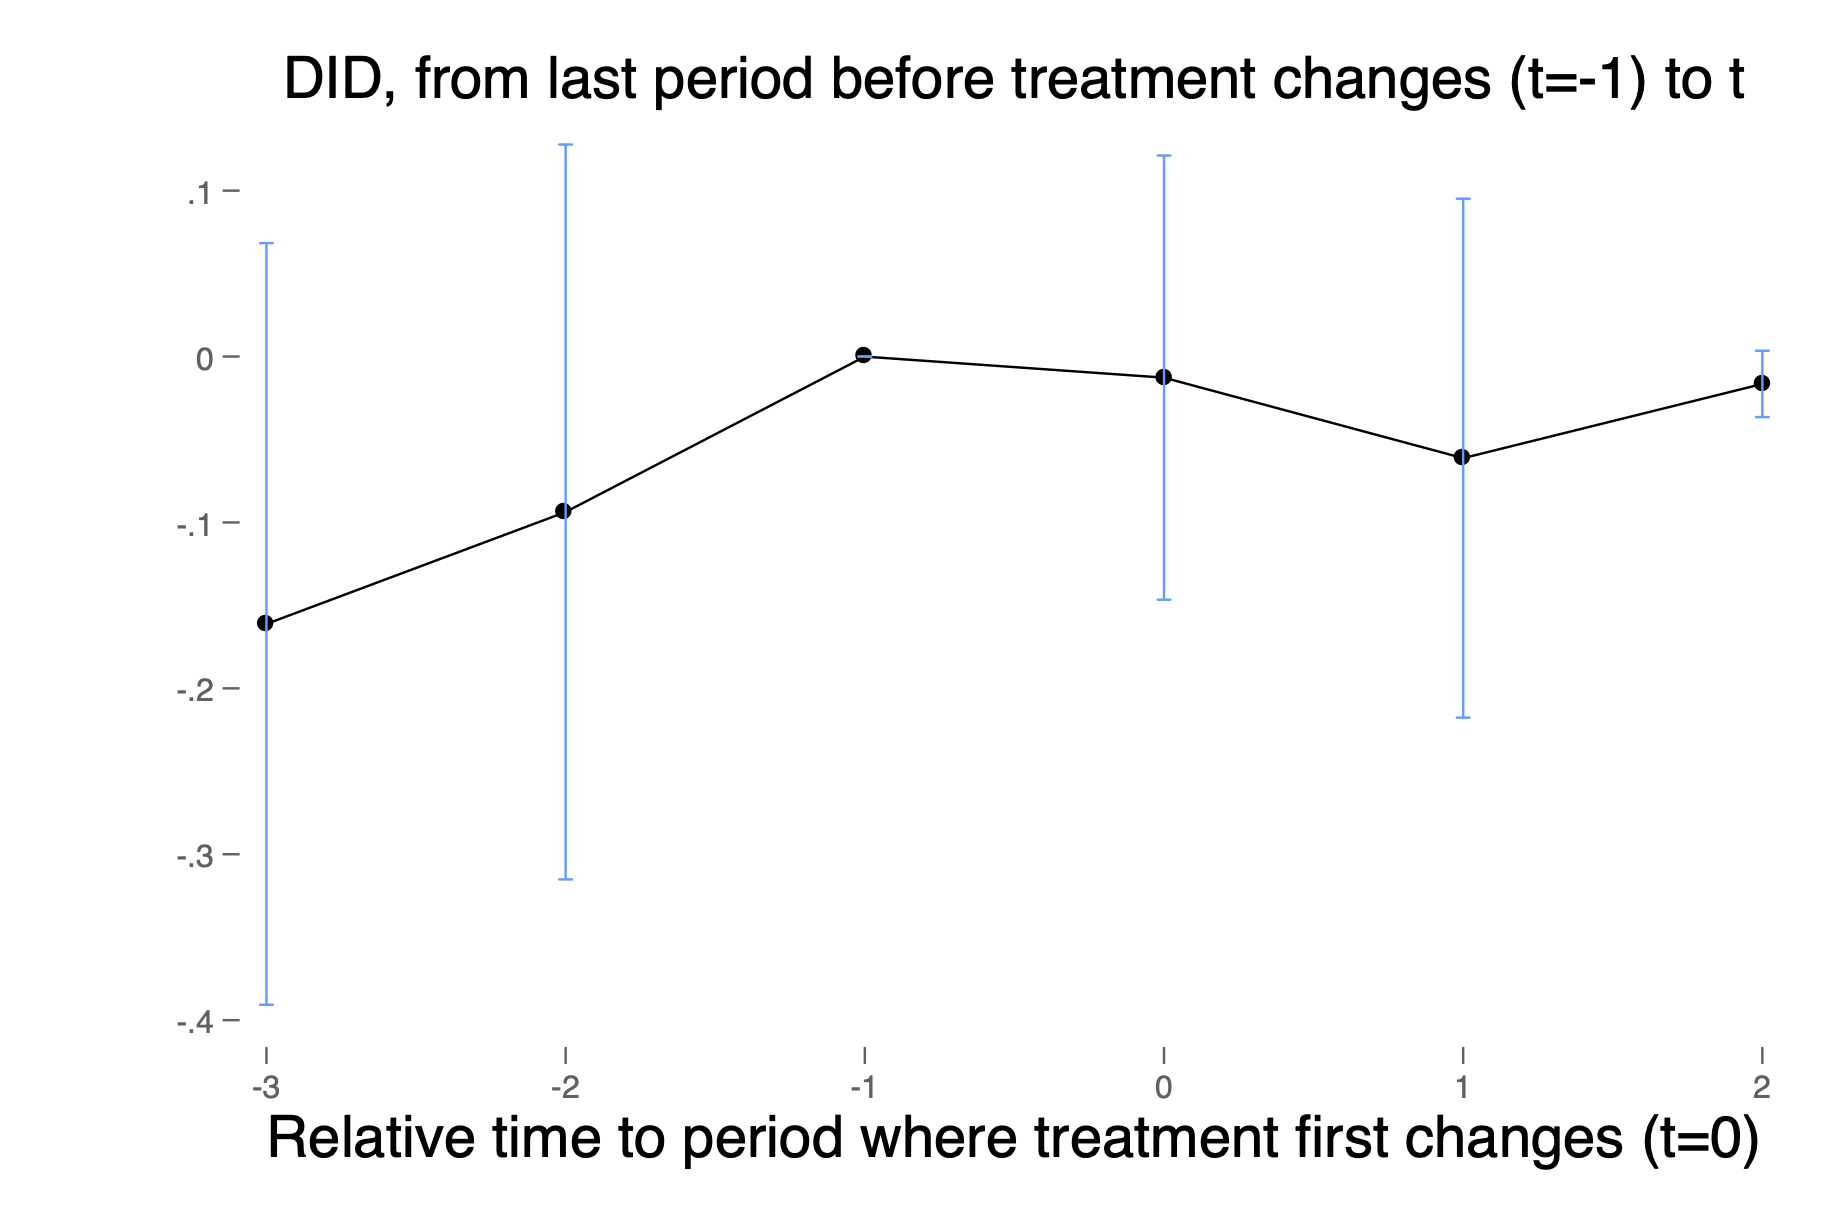
\includegraphics[width=0.9\textwidth]{Chapter1/Figures/chaisemartin_acuerdo_estcom.png}
       \captionsetup{justification=centering}
\end{figure}   

  %\begin{table}[htbp]\def\sym#1{\ifmmode^{#1}\else\(^{#1}\)\fi}
\centering
\caption{Comparison: Security Cooperation Agreements with Governor vs. Other Actors, 2014-2018}
\label{tab:as_comparison_agreements}
\scalebox{1}{
\begin{tabular}{lcc}
\hline \hline
\\ \multicolumn{3}{l}{Dependent variable: Security Cooperation Agreement}\\
& w/ Governor &  w/ Other Political Actors$^a$\\
& \multicolumn{1}{c}{(1)} & \multicolumn{1}{c}{(2)} \\
\cmidrule(lrr){2-2}  \cmidrule(lrr){3-3}\\
\addlinespace
Lag 4 years &         $ 0.0197^{} $ &      $ -0.0326^{} $  \\
& ($ 0.3292$) & ($ 0.0763 $) \\
Lag 3 years &        $ -0.0102^{***} $ &     $ 0.2193^{} $ \\
& ($ 0.0000$) & ($ 0.2702 $) \\
Lag 2 years &        $ 0.1418^{} $ &    $ -0.0648^{} $  \\
& ($ 0.1318$) & ($ 0.0524 $) \\
Reform, time 0 &        $ 0.0064^{} $ &     $ -0.0089^{} $ \\
& ($ 0.0354$) & ($ 0.0069 $) \\
Lead 1 year &         $ -0.2230^{***} $ &       $ -0.2858^{} $ \\
& ($ 0.0435$) & ($ 0.2610 $) \\
Lead 3 years &        $ -0.5921^{***} $ &     $ 0.1665^{} $ \\
& ($ 0.0708$) & ($ 0.1040 $) \\
\addlinespace
Observations       &                  4,382        &           4,382  \\
R-squared        &              0.6434        &           0.5469   \\
Mun. FEs       &     \checkmark         &  \checkmark    \\
Year. FEs       &     \checkmark         &  \checkmark   \\
Controls$^b$   &      \checkmark       &      \checkmark    \\
Cohort weighted   &   \checkmark       &   \checkmark    \\
WILD CI   &          &       \\
Aggregate effect        &              $-0.2696^{***} $$         &            $0.0796^{} $$   \\
SE (aggregate eff.)        &              (0.0339)       &           (0.0491)   \\
\hline \hline
\multicolumn{3}{p{0.7\textwidth}}{\footnotesize{Notes: Coefficients show IW estimators following \citet{abraham_sun_2020}. Two relative time periods (lag 5 and 1) are removed to avoid collinearity problems noted by \citet{abraham_sun_2020}. Standard errors in parentheses are clustered at the state level, with the following significance-level: $^{***}$ 1\%; $^{**}$ 5\%; and $^*$ 10\%, that refer to two-sided t-test with the null hypothesis equal to 0 for each relative time period. $^a$ Refers primarily to the President but could include Governors and mayors from other states or other municipalities from the same state. $^b$ Pretreatment controls include: governor winning margin; party alignment with the President;  party alignment with the Governor; municipal winning margin; logged population; logged organized crime related deaths; and Cartel presence.}} \\
\end{tabular}
}
\end{table}
   
  
  \begin{table}[htbp]\def\sym#1{\ifmmode^{#1}\else\(^{#1}\)\fi}
\centering
\caption{Effect of 2014 Term Limit Reform on the likelihood of signing Security Cooperation Agreements,  by type}
\label{tab:comparison_fed_estatal}
\scalebox{1}{
\begin{tabular}{lcccc}
\hline \hline
\\ \multicolumn{3}{l}{Dependent variable:}\\
& \multicolumn{2}{c}{Security Cooperation Agreement w/ Governor$^{a}$} & \multicolumn{2}{c}{Security Cooperation Agreement w/ Other$^{b}$} \\
& \multicolumn{1}{c}{(1)} & \multicolumn{1}{c}{(2)} & \multicolumn{1}{c}{(3)} & \multicolumn{1}{c}{(4)} \\
\cmidrule(lrr){2-3}  \cmidrule(lrr){4-5}\\
\addlinespace
t-4 &         $ 0.3497^{} $ &         $ 0.0193^{} $ &     $ -0.2763^{} $ &   $ -0.0326^{} $  \\
& ($ 1.8038$) & ($ 0.3316$) & ($ 0.5842$)  & ($ 0.0761 $) \\
t-3 &         $ -0.7355^{} $ &        $ -0.0102^{***} $  &     $ 0.2469^{} $ &     $ 0.2206^{} $ \\
& ($ 37.4159$) & ($ 0.0000$) & ($ 15.0281$) & ($ 0.2702 $) \\
t-2 &         $ 0.3861^{} $ &        $ 0.1420^{} $  &     $ -0.1496^{} $ &    $ -0.0649^{} $  \\
& ($ 0.3279$) & ($ 0.1323$) & ($ 0.1250$) & ($ 0.0524 $) \\
Reform (t=0) &         $ 0.2233^{***} $ &        $ 0.0065^{} $  &     $ -0.0599^{**} $  &     $ -0.0089^{} $ \\
& ($ 0.0581$) & ($ 0.0353$) & ($ 0.0273$) & ($ 0.0070 $) \\
t+1 &         $ -0.2198^{**} $ &         $ -0.2230^{***} $  &     $ 0.1148^{} $ &       $ -0.2845^{} $ \\
& ($ 0.0930$) & ($ 0.0435$) & ($ 0.0904$) & ($ 0.2602 $) \\
t+3 &         $ -0.5915^{***} $ &        $ -0.5921^{***} $ &     $ 0.1660^{*} $  &     $ 0.1665^{} $ \\
& ($ 0.0783$) & ($ 0.0708$) & ($ 0.0953$) & ($ 0.1040 $) \\
\addlinespace
Observations   &                  4,382     &                  4,382  &                  4,382        &           4,382  \\
R-squared      &              0.6433    &              0.6434   &            0.5469        &           0.5469   \\
Mun. FEs       &     \checkmark         &  \checkmark   &     \checkmark         &  \checkmark   \\
Year. FEs       &     \checkmark         &  \checkmark  &     \checkmark         &  \checkmark   \\
Controls$^b$   &      \checkmark       &      \checkmark   &      \checkmark       &      \checkmark   \\
Cohort weighted   &          &   \checkmark   &          &   \checkmark   \\
WILD CI  &     \checkmark         &  \checkmark   &     \checkmark         &  \checkmark   \\
Aggregate effect     &              $-0.213^{***} $$    &        $-0.2696^{***} $$      &            $0.069^{} $$   &       $0.0796^{} $$   \\
SE (aggregate eff.)      &              0.034   &              0.0339    &              0.045       &           0.0491   \\
\hline \hline
\multicolumn{5}{p{1.2\textwidth}}{\footnotesize{Notes: Coefficients in columns (2) and (4) show IW estimators following \citet{abraham_sun_2020}. In those models, two relative time periods (lag 8 and 1) are removed to avoid collinearity problems noted by \citet{abraham_sun_2020}. Standard errors in parentheses are clustered at the state level, with the following significance-level: $^{***}$ 1\%; $^{**}$ 5\%; and $^*$ 10\%, that refer to two-sided t-test with the null hypothesis equal to 0 for each relative time period. $^a$ Refers to security cooperation agreements signed with the governor only. $^b$ Refers to security cooperation agreements signed with other instituions but not the governor. $^c$ State-level controls include governor winning margin in last pre-treatment election and an indicator of whether the governor's party is the same as the federal incumbent party.}} \\
\end{tabular}
}
\end{table}
   
 
 
\def\sym#1{\ifmmode^{#1}\else\(^{#1}\)\fi}
\begin{table}[htbp]\def\sym#1{\ifmmode^{#1}\else\(^{#1}\)\fi}
\centering
\caption{Test on selection on unobservables}
\label{tab:unobservables}
\begin{tabular}{l*{1}{c}}
\hline \hline
&\multicolumn{1}{c}{(1)}         \\
\addlinespace
Fitted value&      0.1312         \\
            &    (0.0780)         \\
\addlinespace
Observations&      10,668         \\
R2          &       0.459         \\
Mun. FE     &      \checkmark               \\
Year FE     &      \checkmark               \\
State Cluster S.E.&     \checkmark                \\
\hline \hline 
\multicolumn{2}{p{0.4\textwidth}}{\footnotesize{Notes: I follow \citet{altonji_etal_2005} to check if unobserved variation is likely to explain the signing of security cooperation agreements with the Governor by mayors. To do so, I regress the treatment (whether the municipality held reelection) on all the available covariates used for Figure \ref{fig:event_study_agreements}.} I then take the fitted value from the regression and use it to predict each outcome, this time including unit and year fixed effects. This test suggests that – under the assumption that observables are representative of unobservables – selection on unobservables is not driving the results.} \\
\end{tabular}
\end{table} 

\clearpage 


\begin{comment}
\begin{figure}[H]
\centering
\caption{Effect of Electoral Reform on Security Cooperation Agreement using non parametric methods\\ -95\% confidence intervals-} 
\label{fig:non_did_agreement}
\begin{center} 
\begin{center} 
	{\textbf Figure A: Generalized Synthetic Control following \citet{xu_2016} }
\end{center}
\includegraphics[width=0.55\textwidth]{Chapter1/Figures/gsynth_wcov_acuerdo.png}

\begin{center}
	{\textbf Figure B: Matrix Completion following \citet{Athey, Bayati, Doudchenko, Imbens, and Khosvari}
\end{center}
\includegraphics[width=0.55\textwidth]{Chapter1/Figures/matrix_completion.png}
       \captionsetup{justification=centering}
       \\
 %{\textbf Note: 95\% confidence intervals estimated using 1,000 bootstrap replications.} .   
\end{figure}      
\end{comment}


\clearpage

\subsection{Mechanisms}

\begin{figure}[H] 
\centering
 \caption{Effect of 2014 Term Limit Reform on Motives to Sign Security Agreements w/ Governor}
 \label{fig:motives}
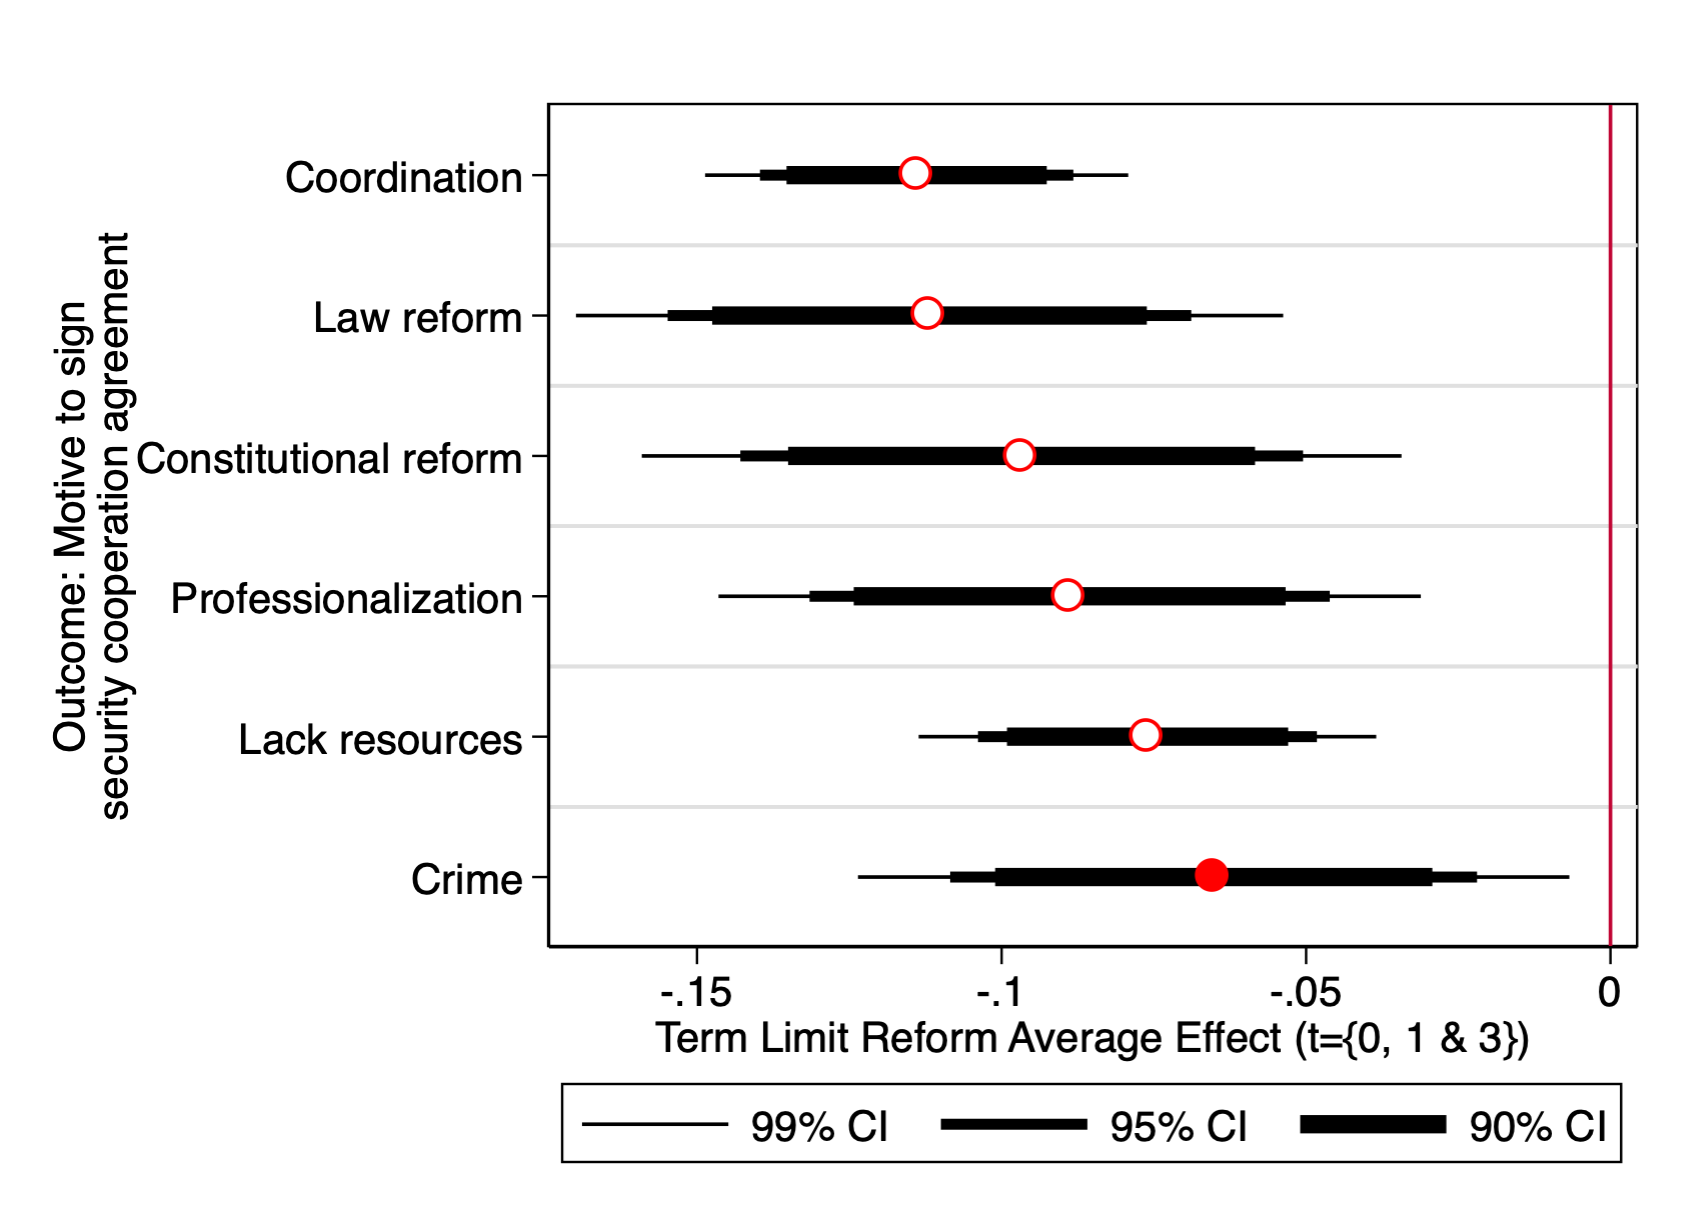
\includegraphics[width=0.9\textwidth]{Chapter1/Figures/motives.png}
       \captionsetup{justification=centering}
\end{figure}   

  \begin{landscape}
\begin{table}[htbp]\def\sym#1{\ifmmode^{#1}\else\(^{#1}\)\fi}
\centering
\caption{Effect of 2014 Term Limit Reform on Motives to Sign Security Agreements w/ Governor}
\label{tab:motives_final}
\scalebox{0.70}{
\begin{tabular}{lcccccc}
\hline \hline
\\ \multicolumn{7}{l}{Dependent variable:}\\
Motive: & Cons. reform  & Law reform & Lack resources & Professionalization & Coordination & Crime \\
& \multicolumn{1}{c}{(1)} & \multicolumn{1}{c}{(2)} & \multicolumn{1}{c}{(3)} & \multicolumn{1}{c}{(4)} & \multicolumn{1}{c}{(5)} & \multicolumn{1}{c}{(6)}  \\
\cmidrule(lrr){2-2}  \cmidrule(lrr){3-3} \cmidrule(lrr){4-4} \cmidrule(lrr){5-5} \cmidrule(lrr){6-6} \cmidrule(lrr){7-7} \\
\addlinespace
t-7 &     $ -0.2350^{***} $ &     $ -0.2581^{**} $ & $ -0.0955^{*} $ & $ -0.2000^{***} $  &     $ -0.1570^{*} $   &     $ -0.1538^{} $ \\
&     ($0.0407$) &     ($0.1175$) & ($0.0484$)& ($ 0.0671$)  &    ($0.0844$)   &   ($0.1078$) \\
t-6 &     $ -0.0758^{***} $ &     $ -0.0876^{***} $ &  $ -0.0615^{***} $ &  $ -0.0647^{} $  &     $ -0.0827^{**} $ &     $ -0.0369^{} $ \\
&     ($0.0176$) &     ($0.0199$) & ($0.0162$)& ($ 0.0585$)  &    ($0.0346$)   &   ($0.0265$) \\
t-5 &     $ 0.0223^{} $ &     $ -0.0405^{} $ &  $ 0.0574^{} $ &  $ 0.0580^{} $ &     $ -0.0106^{} $  &     $ 0.0427^{} $ \\
&     ($0.0591$) &     ($0.0583$) & ($0.0481$)& ($ 0.0750$)  &    ($0.0709$)   &   ($0.0445$) \\
t-4 &     $ 0.0167^{} $ &     $ -0.0832^{} $ &   $ 0.1207^{} $ &   $ 0.0649^{} $  &     $ -0.1313^{} $ &     $ 0.0346^{} $ \\
&     ($0.0987$) &     ($0.0842$) & ($0.0854$)& ($ 0.1053$)  &    ($0.2085$)   &   ($0.1173$) \\
t-3 &     $ -0.0385^{} $ &     $ -0.0160^{} $ &   $ 0.0727^{} $ &   $ 0.0802^{} $  &     $ 0.0403^{} $ &     $ 0.0734^{} $ \\
&     ($0.1052$) &     ($0.0840$) & ($0.1002$)& ($ 0.0738$)  &    ($0.1662$)   &   ($0.1061$) \\
t-2 &     $ -0.1162^{} $ &     $ -0.0914^{} $ &  $ 0.0228^{} $  &  $ -0.0822^{} $  &     $ -0.2796^{*} $ &     $ -0.0753^{} $ \\
&     ($0.1012$) &     ($0.0917$) & ($0.0640$)& ($ 0.1195$)  &    ($0.1379$)   &   ($0.0667$) \\
Reform (t=0) &     $ 0.0457^{} $ &     $ 0.0292^{} $ &   $ 0.0214^{} $   &   $ 0.0282^{} $  &     $ 0.0233^{} $ &     $ 0.0272^{*} $ \\
&     ($0.0278$) &     ($0.0183$) & ($0.0179$)& ($ 0.0201$)  &    ($0.0209$)   &   ($0.0146$) \\
t+1 &     $ -0.0906^{***} $ &     $ -0.1071^{***} $ &    $ -0.0935^{***} $ &    $ -0.0935^{***} $ &     $ -0.1215^{***} $ &     $ -0.0735^{***} $  \\
&     ($0.0164$) &     ($0.0182$) & ($0.0106$)& ($ 0.0160$)  &    ($0.0291$)   &   ($0.0121$) \\
t+3 &     $ -0.2452^{***} $ &     $ -0.2576^{***} $ &   $ -0.1560^{***} $  &   $ -0.2011^{***} $ &     $ -0.2436^{***} $ &     $ -0.1492^{***} $ \\
&     ($0.0535$) &     ($0.0484$) & ($0.0350$)& ($ 0.0463$)  &    ($0.0431$)   &   ($0.0527$) \\
\\
\addlinespace
Observations       &              9,725    &              9,725    &           9,725      &           9,725  &              9,725    &              9,725     \\
R-squared        &          0.2974 &          0.3021    &    0.2617       &           0.2722 &          0.2865 &          0.2594      \\
Mun. FEs      &     \checkmark         &  \checkmark   &     \checkmark         &  \checkmark  &     \checkmark         &  \checkmark   &     \checkmark         &  \checkmark   \\
Year. FEs    &     \checkmark         &  \checkmark   &     \checkmark         &  \checkmark &     \checkmark         &  \checkmark   &     \checkmark         &  \checkmark   \\
Controls$^b$  &    \checkmark     &       \checkmark  &    \checkmark      &   \checkmark &    \checkmark     &       \checkmark  &    \checkmark      &   \checkmark     \\
Cohort weighted  &   \checkmark      &       \checkmark  &   \checkmark       &   \checkmark  &   \checkmark      &       \checkmark  &   \checkmark       &   \checkmark    \\
Reform aggregate effect         & $-0.0967^{***} $$      & $-0.1118^{***} $$    & $-0.0760^{***} $$      & $-0.0888^{***} $$     & $-0.1139^{***} $$      & $-0.0652^{***} $$     \\
SE       & (0.0225)  & (0.0210) & (0.0136)  & (0.0208)  & (0.0125)  & (0.0211)   \\
\hline \hline
\multicolumn{7}{p{1.2\textwidth}}{\footnotesize{Notes: Coefficients show IW estimators following \citet{abraham_sun_2020}. Two relative time periods (lag 8 and 1) are removed to avoid collinearity problems noted by \citet{abraham_sun_2020}. Standard errors in parentheses are clustered at the state level for estimates in saturaded model. Significance-level: $^{***}$ 1\%; $^{**}$ 5\%; and $^*$ 10\%, that refer to two-sided t-test with the null hypothesis equal to 0 for each relative time period. $^a$ Even columns with outcomes with missing values where replaced by zeros assuming no activity was registered. $^b$ State-level controls include governor winning margin in last pre-treatment election and an indicator of whether the governor's party is the same as the federal incumbent party.}} \\
\end{tabular}
}
\end{table}
\end{landscape}
   

   %\begin{landscape}
\begin{table}[htbp]\def\sym#1{\ifmmode^{#1}\else\(^{#1}\)\fi}
\centering
\caption{Effect of 2014 Term Limit Reform on Motives to Sign Security Agreements w/ Governor}
\label{tab:motives_average_final}
\scalebox{0.70}{
\begin{tabular}{lcccccc}
\hline \hline
\\ \multicolumn{7}{l}{Dependent variable:}\\
Motive: & Cons. reform  & Law reform & Lack resources & Professionalization & Coordination & Crime \\
& \multicolumn{1}{c}{(1)} & \multicolumn{1}{c}{(2)} & \multicolumn{1}{c}{(3)} & \multicolumn{1}{c}{(4)} & \multicolumn{1}{c}{(5)} & \multicolumn{1}{c}{(6)}  \\
\cmidrule(lrr){2-2}  \cmidrule(lrr){3-3} \cmidrule(lrr){4-4} \cmidrule(lrr){5-5} \cmidrule(lrr){6-6} \cmidrule(lrr){7-7} \\
\addlinespace
Reform average effect         & $-0.0967^{***} $$      & $-0.1118^{***} $$     & $-0.0760^{***} $$        & $-0.0888^{***} $$       & $-0.1139^{***} $$        & $-0.0652^{***} $$       \\
& (0.0225)  & (0.0210) & (0.0136)  & (0.0208)  & (0.0125)  & (0.0211)   \\
\\
\addlinespace
Observations       &              9,725    &              9,725    &           9,725      &           9,725  &              9,725    &              9,725    \\
R-squared        &          0.2974 &          0.3021    &    0.2617       &           0.2722 &          0.2865 &          0.2594   \\
Mun. FEs      &     \checkmark         &  \checkmark   &     \checkmark         &  \checkmark  &     \checkmark         &  \checkmark   &     \checkmark         &  \checkmark   \\
Year. FEs    &     \checkmark         &  \checkmark   &     \checkmark         &  \checkmark &     \checkmark         &  \checkmark   &     \checkmark         &  \checkmark   \\
Controls$^b$  &    \checkmark     &       \checkmark  &    \checkmark      &   \checkmark &    \checkmark     &       \checkmark  &    \checkmark      &   \checkmark     \\
Cohort weighted  &   \checkmark      &       \checkmark  &   \checkmark       &   \checkmark  &   \checkmark      &       \checkmark  &   \checkmark       &   \checkmark    \\
Parallel trend holds &   \checkmark      &       \checkmark  &   \checkmark       &   \checkmark  &   \checkmark      &       \checkmark  &   \checkmark       &   \checkmark    \\
\hline \hline
\multicolumn{7}{p{1.2\textwidth}}{\footnotesize{Notes: Coefficients show IW estimators following \citet{abraham_sun_2020}. Two relative time periods (lag 8 and 1) are removed to avoid collinearity problems noted by \citet{abraham_sun_2020}. Standard errors in parentheses are clustered at the state level for estimates in saturaded model. Significance-level: $^{***}$ 1\%; $^{**}$ 5\%; and $^*$ 10\%, that refer to two-sided t-test with the null hypothesis equal to 0 for each relative time period. $^a$ Even columns with outcomes with missing values where replaced by zeros assuming no activity was registered. $^b$ State-level controls include governor winning margin in last pre-treatment election and an indicator of whether the governor's party is the same as the federal incumbent party.}} \\
\end{tabular}
}
\end{table}
\end{landscape}
  
   
   
      
\begin{landscape}
\begin{table}[htbp]\def\sym#1{\ifmmode^{#1}\else\(^{#1}\)\fi}
\centering
\caption{Effect of 2014 Term Limit Reform on Services Delegated to the Governor}
\label{tab:services}
\scalebox{0.70}{
\begin{tabular}{lcccccccc}
\hline \hline
\\ \multicolumn{9}{l}{Dependent variable:}\\
Service delegated: & Public security  & Traffic & Prevention & Training  & Technology & Research & Inteligence & Unify procedures \\
& \multicolumn{1}{c}{(1)} & \multicolumn{1}{c}{(2)} & \multicolumn{1}{c}{(3)} & \multicolumn{1}{c}{(4)} & \multicolumn{1}{c}{(5)} & \multicolumn{1}{c}{(6)} & \multicolumn{1}{c}{(7)} & \multicolumn{1}{c}{(8)} \\
\cmidrule(lrr){2-2}  \cmidrule(lrr){3-3} \cmidrule(lrr){4-4} \cmidrule(lrr){5-5} \cmidrule(lrr){6-6} \cmidrule(lrr){7-7} \cmidrule(lrr){8-8} \cmidrule(lrr){9-9} \\
\addlinespace
t-2 &     $ -0.0244^{} $ &     $ -0.0441^{} $ &  $ -0.0598^{***} $  &  $ -0.0565^{***} $  &     $ -0.0567^{***} $ &     $ -0.0596^{***} $ & $ -0.0596^{***} $ & $ -0.0506^{***} $   \\
&     ($0.1046$) &     ($0.0818$) & ($0.0021$)& ($ 0.0012$)  &    ($0.0016$)   &   ($0.0017$) \\
Reform (t=0) &     $ 0.0702^{} $ &     $ 0.0256^{} $ &   $ 0.0175^{} $   &   $ 0.0214^{} $  &     $ 0.0194^{} $ &     $ 0.0194^{} $ & $ 0.0204^{} $ & $ 0.0233^{} $   \\
&     ($0.0436$) &     ($0.0369$) & ($0.0137$)& ($ 0.0142$)  &    ($0.0126$)   &   ($0.0138$) \\
t+1 &     $ -0.0947^{*} $ &     $ -0.0259^{*} $ &    $ 0.0106^{} $ &    $ 0.0053^{} $ &     $ 0.0047^{} $ &     $ 0.0024^{} $  & $ 0.0018^{} $ & $ 0.0053^{} $   \\
&     ($0.0509$) &     ($0.0147$) & ($0.0198$)& ($ 0.0193$)  &    ($0.0197$)   &   ($0.0201$) \\
t+3 &     $ -0.2847^{***} $ &     $ 0.0000^{} $  \\
&     ($0.0430$) &     ($0.0000$)  \\
\\
\addlinespace
Observations       &              4,865    &              4,865    &           3,244      &           3,244  &              3,244    &              3,244  &              3,244    &              6,481   \\
R-squared        &          0.4234 &          0.3703    &    0.5567       &           0.5477 &          0.5409 &          0.5473     &        0.5467    &        0.4894   \\
Mun. FEs      &     \checkmark         &  \checkmark   &     \checkmark         &  \checkmark  &     \checkmark         &  \checkmark   &     \checkmark         &  \checkmark   \\
Year. FEs    &     \checkmark         &  \checkmark   &     \checkmark         &  \checkmark &     \checkmark         &  \checkmark   &     \checkmark         &  \checkmark   \\
Controls$^b$  &    \checkmark     &       \checkmark  &    \checkmark      &   \checkmark &    \checkmark     &       \checkmark  &    \checkmark      &   \checkmark     \\
Cohort weighted  &   \checkmark      &       \checkmark  &   \checkmark       &   \checkmark  &   \checkmark      &       \checkmark  &   \checkmark       &   \checkmark    \\
Reform average effect         & $-0.1031^{***} $$      & $-0.0242^{} $$     & $0.0094^{} $$        & $0.0133^{} $$       & $0.0121^{} $$        & $0.0109^{} $$    & $0.0111^{} $$      & $0.0143^{} $$     \\
SE (average effect)      & (0.0225)  & (0.0162) & (0.0080)  & (0.0120)  & (0.0117)  & (0.0122)    & (0.0123)  & (0.0114)   \\
\hline \hline
\multicolumn{9}{p{1.5\textwidth}}{\footnotesize{Notes: Coefficients show IW estimators following \citet{abraham_sun_2020}. Two relative time periods (lag 8 and 1) are removed to avoid collinearity problems noted by \citet{abraham_sun_2020}. Standard errors in parentheses are clustered at the state level for estimates in saturaded model. Significance-level: $^{***}$ 1\%; $^{**}$ 5\%; and $^*$ 10\%, that refer to two-sided t-test with the null hypothesis equal to 0 for each relative time period. $^a$ Even columns with outcomes with missing values where replaced by zeros assuming no activity was registered. $^b$ State-level controls include governor winning margin in last pre-treatment election and an indicator of whether the governor's party is the same as the federal incumbent party.}} \\
\end{tabular}
}
\end{table}
\end{landscape}
   
%\begin{landscape}
\begin{table}[htbp]\def\sym#1{\ifmmode^{#1}\else\(^{#1}\)\fi}
\centering
\caption{Effect of 2014 Term Limit Reform on Services Delegated to the Governor}
\label{tab:services_average}
\scalebox{0.70}{
\begin{tabular}{lcccccccc}
\hline \hline
\\ \multicolumn{9}{l}{Dependent variable:}\\
Service delegated: & Public security  & Traffic & Prevention & Training  & Technology & Research & Inteligence & Unify procedures \\
& \multicolumn{1}{c}{(1)} & \multicolumn{1}{c}{(2)} & \multicolumn{1}{c}{(3)} & \multicolumn{1}{c}{(4)} & \multicolumn{1}{c}{(5)} & \multicolumn{1}{c}{(6)} & \multicolumn{1}{c}{(7)} & \multicolumn{1}{c}{(8)} \\
\cmidrule(lrr){2-2}  \cmidrule(lrr){3-3} \cmidrule(lrr){4-4} \cmidrule(lrr){5-5} \cmidrule(lrr){6-6} \cmidrule(lrr){7-7} \cmidrule(lrr){8-8} \cmidrule(lrr){9-9} \\
\addlinespace
Reform average effect         & $0.0149^{*} $$      & $0.0579^{***} $$     & $0.0426^{***} $$        & $0.0034^{} $$       & $-0.0345^{***} $$        & $-0.0819^{***} $$    & $0.0092^{} $$      & $0.0056^{} $$     \\
SE       & (0.0079)  & (0.0099) & (0.0046)  & (0.0048)  & (0.0103)  & (0.0085)    & (0.0063)  & (0.0034)   \\
\addlinespace
Observations       &             11,353    &             11,353    &          11,353      &          11,353  &             11,353    &             11,353  &             11,353    &             11,353   \\
R-squared        &          0.8662 &          0.8556    &    0.9239       &           0.8767 &          0.8548 &          0.8954     &        0.8557    &        0.7008   \\
Mun. FEs      &     \checkmark         &  \checkmark   &     \checkmark         &  \checkmark  &     \checkmark         &  \checkmark   &     \checkmark         &  \checkmark   \\
Year. FEs    &     \checkmark         &  \checkmark   &     \checkmark         &  \checkmark &     \checkmark         &  \checkmark   &     \checkmark         &  \checkmark   \\
Controls$^b$  &    \checkmark     &       \checkmark  &    \checkmark      &   \checkmark &    \checkmark     &       \checkmark  &    \checkmark      &   \checkmark     \\
Cohort weighted  &   \checkmark      &       \checkmark  &   \checkmark       &   \checkmark  &   \checkmark      &       \checkmark  &   \checkmark       &   \checkmark    \\
Parallel trend holds &   \checkmark      &       \checkmark  &          &     &         &       &          &       \\
\hline \hline
\multicolumn{9}{p{1.5\textwidth}}{\footnotesize{Notes: Coefficients show IW estimators following \citet{abraham_sun_2020}. Two relative time periods (lag 8 and 1) are removed to avoid collinearity problems noted by \citet{abraham_sun_2020}. Standard errors in parentheses are clustered at the state level for estimates in saturaded model. Significance-level: $^{***}$ 1\%; $^{**}$ 5\%; and $^*$ 10\%, that refer to two-sided t-test with the null hypothesis equal to 0 for each relative time period. $^a$ Even columns with outcomes with missing values where replaced by zeros assuming no activity was registered. $^b$ State-level controls include governor winning margin in last pre-treatment election and an indicator of whether the governor's party is the same as the federal incumbent party.}} \\
\end{tabular}
}
\end{table}
\end{landscape}
   

\begin{landscape}
\begin{table}[htbp]\def\sym#1{\ifmmode^{#1}\else\(^{#1}\)\fi}
\centering
\caption{Effect of 2014 Term Limit Reform on Services Delegated to the Governor}
\label{tab:interaction_alignment}
\scalebox{0.70}{
\begin{tabular}{lccc}
\hline \hline
\\ \multicolumn{4}{l}{Dependent variable: Signing Security Cooperation Agreement w/ Governor}\\
Alignment: & w/ President  & w/ Governor  & w/ Governor from PRI \\
& \multicolumn{1}{c}{(1)} & \multicolumn{1}{c}{(2)} & \multicolumn{1}{c}{(3)} \\
\cmidrule(lrr){2-2}  \cmidrule(lrr){3-3} \cmidrule(lrr){4-4} \\
\addlinespace
t-7 &     $ -0.2383^{*} $ &     $ -0.0191^{*} $ &  $ 0.0000^{} $ \\
&     ($0.1348$) &     ($0.0108$) & ($0.0000$) \\
t-6 &     $ -0.0807^{} $ &     $ 0.0199^{} $ &  $ -0.0430^{} $  \\
&     ($0.0873$) &     ($0.0499$) & ($0.0467$) \\
t-5 &     $ -0.1186^{} $ &     $ -0.2028^{**} $ &  $ -0.2406^{**} $  \\
&     ($0.1046$) &     ($0.0924$) & ($0.0922$) \\
t-4 &     $ 0.0665^{} $ &     $ -0.0784^{} $ &  $ -0.1077^{} $  \\
&     ($0.1483$) &     ($0.1203$) & ($0.1236$) \\
t-3 &     $ 0.3395^{**} $ &     $ 0.2569^{***} $ &  $ 0.2303^{***} $  \\
&     ($0.1651$) &     ($0.0720$) & ($0.0702$) \\
t-2 &     $ 0.0027^{} $ &     $ -0.0253^{} $ &  $ 0.0976^{} $  \\
&     ($0.1572$) &     ($0.1182$) & ($0.1471$) \\
Reform (t=0) &     $ -0.1686^{} $ &     $ -0.2236^{} $ &   $ 0.1790^{} $   \\
&     ($0.1877$) &     ($0.1316$) & ($0.1258$) \\
t+1 &     $ -0.2169^{} $ &     $ -0.5692^{**} $ &    $ -0.0199^{} $ \\
&     ($0.1884$) &     ($0.2119$) & ($0.1549$) \\
t+2 &     $ -0.1125^{} $ &     $ -0.5020^{*} $  &     $ -0.4753^{*} $ \\
&     ($0.2496$) &     ($0.2690$)  & ($0.2741$) \\
t+3 &     $ -0.2197^{} $ &     $ -0.3562^{} $  &     $ -0.3876^{} $ \\
&     ($0.2241$) &     ($0.3827$)  & ($0.3818$) \\
\\
\addlinespace
Observations       &             12,173    &             12,173    &          12,173    \\
R-squared        &          0.4555 &          0.4566    &    0.4541    \\
Mun. FEs      &     \checkmark         &  \checkmark   &     \checkmark    \\
Year. FEs    &     \checkmark         &  \checkmark   &     \checkmark    \\
Controls$^b$  &    \checkmark     &       \checkmark  &    \checkmark   \\
Cohort weighted  &   \checkmark      &       \checkmark  &   \checkmark    \\
Reform average effect         & $-0.1376^{} $$      & $-0.1538^{*} $$     & $-0.0551^{} $$     \\
SE (average effect)      & (0.1313)  & (0.0906) & (0.0652) \\
\hline \hline
\multicolumn{4}{p{1.5\textwidth}}{\footnotesize{Notes: Coefficients show IW estimators following \citet{abraham_sun_2020}. Two relative time periods (lag 8 and 1) are removed to avoid collinearity problems noted by \citet{abraham_sun_2020}. Standard errors in parentheses are clustered at the state level for estimates in saturaded model. Significance-level: $^{***}$ 1\%; $^{**}$ 5\%; and $^*$ 10\%, that refer to two-sided t-test with the null hypothesis equal to 0 for each relative time period. $^a$ Even columns with outcomes with missing values where replaced by zeros assuming no activity was registered. $^b$ State-level controls include governor winning margin in last pre-treatment election and an indicator of whether the governor's party is the same as the federal incumbent party.}} \\
\end{tabular}
}
\end{table}
\end{landscape}
   
%\begin{landscape}
\begin{table}[htbp]\def\sym#1{\ifmmode^{#1}\else\(^{#1}\)\fi}
\centering
\caption{Effect of 2014 Term Limit Reform on Services Delegated to the Governor}
\label{tab:interaction_alignment_average}
\scalebox{0.70}{
\begin{tabular}{lccc}
\hline \hline
\\ \multicolumn{4}{l}{Dependent variable: Signing Security Cooperation Agreement w/ Governor}\\
Alignment: & w/ President  & w/ Governor  & w/ Governor from PRI \\
& \multicolumn{1}{c}{(1)} & \multicolumn{1}{c}{(2)} & \multicolumn{1}{c}{(3)} \\
\cmidrule(lrr){2-2}  \cmidrule(lrr){3-3} \cmidrule(lrr){4-4} \\
\addlinespace
Reform average effect         & $-0.1376^{} $$      & $-0.1538^{*} $$     & $-0.0551^{} $$     \\
& (0.1313)  & (0.0906) & (0.0652) \\
\\
\addlinespace
Observations       &             12,173    &             12,173    &          12,173    \\
R-squared        &          0.4555 &          0.4566    &    0.4541    \\
Mun. FEs      &     \checkmark         &  \checkmark   &     \checkmark    \\
Year. FEs    &     \checkmark         &  \checkmark   &     \checkmark    \\
Controls$^b$  &    \checkmark     &       \checkmark  &    \checkmark   \\
Cohort weighted  &   \checkmark      &       \checkmark  &   \checkmark    \\
\hline \hline
\multicolumn{4}{p{1.5\textwidth}}{\footnotesize{Notes: Coefficients show IW estimators following \citet{abraham_sun_2020}. Two relative time periods (lag 8 and 1) are removed to avoid collinearity problems noted by \citet{abraham_sun_2020}. Standard errors in parentheses are clustered at the state level for estimates in saturaded model. Significance-level: $^{***}$ 1\%; $^{**}$ 5\%; and $^*$ 10\%, that refer to two-sided t-test with the null hypothesis equal to 0 for each relative time period. $^a$ Even columns with outcomes with missing values where replaced by zeros assuming no activity was registered. $^b$ State-level controls include governor winning margin in last pre-treatment election and an indicator of whether the governor's party is the same as the federal incumbent party.}} \\
\end{tabular}
}
\end{table}
\end{landscape}
   

              
\begin{landscape}
\begin{table}[htbp]\def\sym#1{\ifmmode^{#1}\else\(^{#1}\)\fi}
\centering
\caption{Reform interaction with citizens' preferences}
\label{tab:interaction_trust}
\scalebox{0.70}{
\begin{tabular}{lcccccccc}
\hline \hline
\\ \multicolumn{9}{l}{Dependent variable: Signing Security Cooperation Agreement w/ Governor}\\
Jurisdiction: & \multicolumn{2}{c}{Municipal} & \multicolumn{2}{c}{State} & \multicolumn{4}{c}{Federal} \\
Trust in Police Force: & Traffic  & Preventive  & State Police & State Attorney Police & Federal Police & Ministerial Police & Army & Marines \\
& \multicolumn{1}{c}{(1)} & \multicolumn{1}{c}{(2)} & \multicolumn{1}{c}{(3)} & \multicolumn{1}{c}{(4)} & \multicolumn{1}{c}{(5)} & \multicolumn{1}{c}{(6)} & \multicolumn{1}{c}{(7)} & \multicolumn{1}{c}{(8)} \\
\cmidrule(lrr){2-2}  \cmidrule(lrr){3-3} \cmidrule(lrr){4-4} \cmidrule(lrr){5-5} \cmidrule(lrr){6-6} \cmidrule(lrr){7-7} \cmidrule(lrr){8-8} \cmidrule(lrr){9-9} \\
\addlinespace
t-7 &     $ 0.1781^{} $ &     $ 0.0000^{} $ &  $ 0.1737^{} $  &  $ 0.1269^{} $  &     $ 0.0908^{} $ &     $ 0.1162^{} $ & $ 0.1093^{*} $ & $ 0.0788^{} $   \\
&     ($0.1657$) &     ($0.0000$) & ($0.1372$)& ($ 0.1137$)  &    ($0.0736$)   &   ($0.0858$) &    ($0.0638$)   &   ($0.0557$) \\
t-6 &     $ -0.0459^{} $ &     $ -0.0601^{} $ &  $ -0.0415^{} $  &  $ -0.0566^{} $  &     $ 0.0056^{} $ &     $ -0.0538^{} $ & $ 0.0234^{} $ & $ 0.0038^{} $   \\
&     ($0.0801$) &     ($0.0481$) & ($0.0539$)& ($ 0.0457$)  &    ($0.0390$)   &   ($0.0379$) &    ($0.0413$)   &   ($0.0413$) \\
t-5 &     $ -0.8924^{***} $ &     $ -0.2958^{} $ &  $ -0.7754^{} $  &  $ -1.3248^{} $  &     $ -0.8583^{**} $ &     $ -1.3845^{***} $ & $ -0.6699^{**} $ & $ -0.5789^{} $   \\
&     ($0.2538$) &     ($0.2471$) & ($0.6290$)& ($ 0.9127$)  &    ($0.3310$)   &   ($0.2852$) &    ($0.3135$)   &   ($0.3456$) \\
t-4 &     $ -0.8378^{} $ &     $ -0.4847^{} $ &  $ -0.8334^{} $  &  $ -1.8134^{} $  &     $ -1.0907^{} $ &     $ -1.2390^{} $ & $ -0.3788^{} $ & $ -0.4918^{} $   \\
&     ($0.7686$) &     ($0.7828$) & ($0.7594$)& ($ 1.3211$)  &    ($0.7492$)   &   ($1.0418$) &    ($0.5581$)   &   ($0.6697$) \\
t-3 &     $ -0.0583^{} $ &     $ -0.2255^{} $ &  $ -0.4855^{} $  &  $ -1.8474^{} $  &     $ -0.6963^{} $ &     $ -0.8293^{} $ & $ 0.1189^{} $ & $ -0.1128^{} $   \\
&     ($0.8134$) &     ($0.8597$) & ($0.7510$)& ($ 1.3390$)  &    ($0.8562$)   &   ($1.1144$) &    ($0.6286$)   &   ($0.7221$) \\
t-2 &     $ 0.0349^{} $ &     $ -0.2669^{} $ &  $ -0.2886^{} $  &  $ -0.6193^{} $  &     $ -0.6132^{} $ &     $ -0.3460^{} $ & $ -0.4240^{} $ & $ -0.4018^{} $   \\
&     ($0.5384$) &     ($0.5922$) & ($0.4176$)& ($ 0.8964$)  &    ($0.4795$)   &   ($0.7851$) &    ($0.3186$)   &   ($0.4479$) \\
Reform (t=0) &     $ -0.4445^{} $ &     $ 0.1161^{} $ &   $ -0.5433^{} $   &   $ -0.3590^{} $  &     $ -1.2945^{**} $ &     $ -0.8582^{} $ & $ -0.4517^{} $ & $ -0.8450^{} $   \\
&     ($0.4490$) &     ($0.4974$) & ($0.4116$)& ($ 1.1629$)  &    ($0.5674$)   &   ($0.7679$) &    ($0.4624$)   &   ($0.5361$) \\
t+1 &     $ -0.9837^{} $ &     $ -0.2187^{} $ &    $ -1.3877^{**} $ &    $ -1.3448^{} $ &     $ -2.4944^{***} $ &     $ -1.8551^{*} $  & $ -1.5411^{**} $ & $ -1.8923^{**} $   \\
&     ($0.5947$) &     ($0.5769$) & ($0.6053$)& ($ 1.4393$)  &    ($0.7475$)   &   ($0.9450$) &    ($0.6971$)   &   ($0.6934$) \\
t+2 &     $ -1.8509^{***} $ &     $ -1.6314^{**} $ &    $ -1.9022^{**} $ &    $ -4.0615^{***} $ &     $ -2.2753^{***} $ &     $ -3.3031^{***} $  & $ -1.2009^{} $ & $ -1.8294^{**} $   \\
&     ($0.5939$) &     ($0.6872$) & ($0.8555$)& ($ 1.1352$)  &    ($0.7941$)   &   ($0.6820$) &    ($0.7654$)   &   ($0.6810$) \\
t+3 &     $ -0.1382^{} $ &     $ -1.5280^{} $ &    $ -0.9653^{} $ &    $ -1.9755^{*} $ &     $ -0.9980^{} $ &     $ -1.1886^{} $  & $ 0.0385^{} $ & $ -0.9525^{} $   \\
&     ($1.1166$) &     ($1.1456$) & ($0.7908$)& ($ 1.0802$)  &    ($1.4571$)   &   ($1.2863$) &    ($1.1601$)   &   ($1.1245$) \\
\\
\addlinespace
Observations       &             12,173    &             12,173    &          12,173      &          12,173  &             12,173    &             12,173  &             12,173    &             12,173   \\
R-squared        &          0.4666 &          0.4641    &    0.4675       &           0.4673 &          0.4642 &          0.4719     &        0.4666    &        0.4666   \\
Mun. FEs      &     \checkmark         &  \checkmark   &     \checkmark         &  \checkmark  &     \checkmark         &  \checkmark   &     \checkmark         &  \checkmark   \\
Year. FEs    &     \checkmark         &  \checkmark   &     \checkmark         &  \checkmark &     \checkmark         &  \checkmark   &     \checkmark         &  \checkmark   \\
Controls$^b$  &    \checkmark     &       \checkmark  &    \checkmark      &   \checkmark &    \checkmark     &       \checkmark  &    \checkmark      &   \checkmark     \\
Cohort weighted  &   \checkmark      &       \checkmark  &   \checkmark       &   \checkmark  &   \checkmark      &       \checkmark  &   \checkmark       &   \checkmark    \\
Reform average effect         & $-0.1400^{} $$      & $-0.2053^{} $$     & $-0.3431^{**} $$        & $-0.2984^{**} $$       & $-0.5739^{**} $$        & $-0.2614^{**} $$    & $-0.4636^{} $$      & $-0.4837^{*} $$     \\
SE (average effect)      & (0.0944)  & (0.1633) & (0.1594)  & (0.1455)  & (0.2673)  & (0.1107)    & (0.4248)  & (0.2374)   \\
\hline \hline
\multicolumn{9}{p{1.8\textwidth}}{\footnotesize{Notes: Coefficients show IW estimators following \citet{abraham_sun_2020}. Two relative time periods (lag 8 and 1) are removed to avoid collinearity problems noted by \citet{abraham_sun_2020}. Standard errors in parentheses are clustered at the state level, with the following significance-level: $^{***}$ 1\%; $^{**}$ 5\%; and $^*$ 10\%, that refer to two-sided t-test with the null hypothesis equal to 0 for each relative time period. $^a$ Refers to security cooperation agreements signed with the Governor. $^b$ Pretreatment controls include: governor winning margin; party alignment with the President;  party alignment with the Governor; municipal winning margin; logged population; logged organized crime related deaths; and Cartel presence.}} \\
\end{tabular}
}
\end{table}
\end{landscape}
   
%\begin{landscape}
\begin{table}[htbp]\def\sym#1{\ifmmode^{#1}\else\(^{#1}\)\fi}
\centering
\caption{Reform interaction with citizens' preferences}
\label{tab:interaction_trust_average}
\scalebox{0.70}{
\begin{tabular}{lcccccccc}
\hline \hline
\\ \multicolumn{9}{l}{Dependent variable: Signing Security Cooperation Agreement w/ Governor}\\
Jurisdiction: & \multicolumn{2}{c}{Municipal} & \multicolumn{2}{c}{State} & \multicolumn{4}{c}{Federal} \\
Trust in Police Force: & Traffic  & Preventive  & State Police & State Attorney Police & Federal Police & Ministerial Police & Army & Marines \\
& \multicolumn{1}{c}{(1)} & \multicolumn{1}{c}{(2)} & \multicolumn{1}{c}{(3)} & \multicolumn{1}{c}{(4)} & \multicolumn{1}{c}{(5)} & \multicolumn{1}{c}{(6)} & \multicolumn{1}{c}{(7)} & \multicolumn{1}{c}{(8)} \\
\cmidrule(lrr){2-2}  \cmidrule(lrr){3-3} \cmidrule(lrr){4-4} \cmidrule(lrr){5-5} \cmidrule(lrr){6-6} \cmidrule(lrr){7-7} \cmidrule(lrr){8-8} \cmidrule(lrr){9-9} \\
\addlinespace
Reform average effect         & $-0.1400^{} $$      & $-0.2053^{} $$     & $-0.3431^{**} $$        & $-0.2984^{**} $$       & $-0.5739^{**} $$        & $-0.2614^{**} $$    & $-0.4636^{} $$      & $-0.4837^{*} $$     \\
SE (average effect)      & (0.0944)  & (0.1633) & (0.1594)  & (0.1455)  & (0.2673)  & (0.1107)    & (0.4248)  & (0.2374)   \\
\\
\addlinespace
Observations       &             12,173    &             12,173    &          12,173      &          12,173  &             12,173    &             12,173  &             12,173    &             12,173   \\
R-squared        &          0.4666 &          0.4641    &    0.4675       &           0.4673 &          0.4642 &          0.4719     &        0.4666    &        0.4666   \\
Mun. FEs      &     \checkmark         &  \checkmark   &     \checkmark         &  \checkmark  &     \checkmark         &  \checkmark   &     \checkmark         &  \checkmark   \\
Year. FEs    &     \checkmark         &  \checkmark   &     \checkmark         &  \checkmark &     \checkmark         &  \checkmark   &     \checkmark         &  \checkmark   \\
Controls$^b$  &    \checkmark     &       \checkmark  &    \checkmark      &   \checkmark &    \checkmark     &       \checkmark  &    \checkmark      &   \checkmark     \\
Cohort weighted  &   \checkmark      &       \checkmark  &   \checkmark       &   \checkmark  &   \checkmark      &       \checkmark  &   \checkmark       &   \checkmark    \\
\hline \hline
\multicolumn{9}{p{1.5\textwidth}}{\footnotesize{Notes: Coefficients show IW estimators following \citet{abraham_sun_2020}. Two relative time periods (lag 8 and 1) are removed to avoid collinearity problems noted by \citet{abraham_sun_2020}. Standard errors in parentheses are clustered at the state level, with the following significance-level: $^{***}$ 1\%; $^{**}$ 5\%; and $^*$ 10\%, that refer to two-sided t-test with the null hypothesis equal to 0 for each relative time period. $^a$ Refers to security cooperation agreements signed with the Governor. $^b$ Pretreatment controls include: governor winning margin; party alignment with the President;  party alignment with the Governor; municipal winning margin; logged population; logged organized crime related deaths; and Cartel presence.}} \\
\end{tabular}
}
\end{table}
\end{landscape}
   
 
\begin{landscape}
\begin{table}[htbp]\def\sym#1{\ifmmode^{#1}\else\(^{#1}\)\fi}
\centering
\caption{Reform interaction with citizens' being able to identify a Police Force}
\label{tab:interaction_identify}
\scalebox{0.70}{
\begin{tabular}{lcccccccc}
\hline \hline
\\ \multicolumn{9}{l}{Dependent variable: Signing Security Cooperation Agreement w/ Governor}\\
Jurisdiction: & \multicolumn{2}{c}{Municipal} & \multicolumn{2}{c}{State} & \multicolumn{4}{c}{Federal} \\
Identify Policy Force: & Traffic  & Preventive  & State Police & State Attorney Police & Federal Police & Ministerial Police & Army & Marines \\
& \multicolumn{1}{c}{(1)} & \multicolumn{1}{c}{(2)} & \multicolumn{1}{c}{(3)} & \multicolumn{1}{c}{(4)} & \multicolumn{1}{c}{(5)} & \multicolumn{1}{c}{(6)} & \multicolumn{1}{c}{(7)} & \multicolumn{1}{c}{(8)} \\
\cmidrule(lrr){2-2}  \cmidrule(lrr){3-3} \cmidrule(lrr){4-4} \cmidrule(lrr){5-5} \cmidrule(lrr){6-6} \cmidrule(lrr){7-7} \cmidrule(lrr){8-8} \cmidrule(lrr){9-9} \\
\addlinespace
t-7 &     $ -0.8572^{} $ &     $ 0.1007^{} $ &  $ 0.0649^{} $  &  $ 0.0783^{} $  &     $ -2.5321^{***} $ &     $ 0.0632^{} $ & $ -1.4640^{*} $ & $ 0.0539^{} $   \\
&     ($0.6544$) &     ($0.0978$) & ($0.0611$)& ($ 0.0697$)  &    ($0.8962$)   &   ($0.0550$) &    ($0.8372$)   &   ($0.0455$) \\
t-6 &     $ -0.2641^{} $ &     $ 0.0248^{} $ &  $ 0.0135^{} $  &  $ 0.0056^{} $  &     $ -0.7692^{***} $ &     $ -0.0035^{} $ & $ -0.4466^{*} $ & $ 0.0092^{} $   \\
&     ($0.2039$) &     ($0.0609$) & ($0.0467$)& ($ 0.0441$)  &    ($0.2696$)   &   ($0.0413$) &    ($0.2577$)   &   ($0.0423$) \\
t-5 &     $ -0.4097^{} $ &     $ -0.0652^{} $ &  $ 0.6451^{} $  &  $ 0.1762^{} $  &     $ -1.1340^{**} $ &     $ -0.7691^{***} $ & $ -0.8805^{} $ & $ -0.3720^{} $   \\
&     ($0.3986$) &     ($0.3080$) & ($0.3960$)& ($ 0.4004$)  &    ($0.4306$)   &   ($0.2589$) &    ($0.5274$)   &   ($0.2421$) \\
t-4 &     $ 0.3350^{} $ &     $ 0.1050^{} $ &  $ 0.7461^{} $  &  $ -0.0893^{} $  &     $ -1.6040^{***} $ &     $ -0.2211^{} $ & $ -0.7589^{} $ & $ -0.3294^{} $   \\
&     ($0.5455$) &     ($0.5451$) & ($0.4774$)& ($ 0.6583$)  &    ($0.5716$)   &   ($0.7553$) &    ($0.8538$)   &   ($0.4995$) \\
t-3 &     $ 0.8549^{} $ &     $ 0.3354^{} $ &  $ 0.8618^{*} $  &  $ -0.1098^{} $  &     $ -1.2530^{**} $ &     $ 0.2973^{} $ & $ -0.3261^{} $ & $ -0.0407^{} $   \\
&     ($0.5572$) &     ($0.6384$) & ($0.5038$)& ($ 0.7313$)  &    ($0.6065$)   &   ($0.8187$) &    ($0.8829$)   &   ($0.5638$) \\
t-2 &     $ -0.0741^{} $ &     $ 0.0173^{} $ &  $ 0.3106^{} $  &  $ -0.0035^{} $  &     $ -1.1572^{**} $ &     $ -0.2290^{} $ & $ -0.7416^{} $ & $ -0.3552^{} $   \\
&     ($0.3985$) &     ($0.3426$) & ($0.3583$)& ($ 0.4741$)  &    ($0.4705$)   &   ($0.5458$) &    ($0.5501$)   &   ($0.3444$) \\
Reform (t=0) &     $ 0.0965^{} $ &     $ -0.3095^{} $ &   $ -0.6740^{} $   &   $ -0.0176^{} $  &     $ -1.7122^{***} $ &     $ -0.3017^{} $ & $ -0.8230^{} $ & $ -0.7614^{} $   \\
&     ($0.3746$) &     ($0.5580$) & ($0.5072$)& ($ 0.5448$)  &    ($0.5196$)   &   ($0.5185$) &    ($0.5125$)   &   ($0.4724$) \\
t+1 &     $ 0.1452^{} $ &     $ -0.8415^{} $ &    $ -0.5733^{} $ &    $ -0.5894^{} $ &     $ -1.1449^{**} $ &     $ -1.2316^{} $  & $ -0.8753^{} $ & $ -1.6442^{***} $   \\
&     ($0.4015$) &     ($0.7920$) & ($0.6386$)& ($ 0.7035$)  &    ($0.4877$)   &   ($0.7296$) &    ($0.5560$)   &   ($0.5433$) \\
t+2 &     $ 0.4499^{} $ &     $ -0.7212^{} $ &    $ 0.0862^{} $ &    $ -1.4956^{**} $ &     $ -0.5687^{} $ &     $ -1.6626^{**} $  & $ -0.4091^{} $ & $ -1.5000^{**} $   \\
&     ($0.3760$) &     ($0.7799$) & ($0.6272$)& ($ 0.7215$)  &    ($0.5955$)   &   ($0.6266$) &    ($0.6311$)   &   ($0.5652$) \\
t+3 &     $ 1.1277^{} $ &     $ -0.5739^{} $ &    $ -0.6702^{} $ &    $ -1.2519^{} $ &     $ -1.7933^{} $ &     $ 0.0623^{} $  & $ -0.5981^{} $ & $ -1.0885^{} $   \\
&     ($0.9218$) &     ($1.2931$) & ($0.9352$)& ($ 1.0598$)  &    ($1.0758$)   &   ($1.0916$) &    ($0.9325$)   &   ($0.9434$) \\
\\
\addlinespace
Observations       &             12,173    &             12,173    &          12,173      &          12,173  &             12,173    &             12,173  &             12,173    &             12,173   \\
R-squared        &          0.4688 &          0.4599    &    0.4659       &           0.4658 &          0.4624 &          0.4783     &        0.4645    &        0.4655   \\
Mun. FEs      &     \checkmark         &  \checkmark   &     \checkmark         &  \checkmark  &     \checkmark         &  \checkmark   &     \checkmark         &  \checkmark   \\
Year. FEs    &     \checkmark         &  \checkmark   &     \checkmark         &  \checkmark &     \checkmark         &  \checkmark   &     \checkmark         &  \checkmark   \\
Controls$^b$  &    \checkmark     &       \checkmark  &    \checkmark      &   \checkmark &    \checkmark     &       \checkmark  &    \checkmark      &   \checkmark     \\
Cohort weighted  &   \checkmark      &       \checkmark  &   \checkmark       &   \checkmark  &   \checkmark      &       \checkmark  &   \checkmark       &   \checkmark    \\
Reform average effect         & $0.3037^{} $      & $-0.4471^{} $     & $-0.2964^{} $        & $-0.3087^{} $       & $-0.7782^{**} $        & $-0.2768^{} $    & $-0.5017^{} $      & $-0.5781^{**} $     \\
SE (average effect)      & (0.3233)  & (0.6044) & (0.3716)  & (0.2401)  & (0.2868)  & (0.2411)    & (0.4665)  & (0.2669)   \\
\hline \hline
\multicolumn{9}{p{1.6\textwidth}}{\footnotesize{Notes: Coefficients show IW estimators following \citet{abraham_sun_2020}. Two relative time periods (lag 8 and 1) are removed to avoid collinearity problems noted by \citet{abraham_sun_2020}. Standard errors in parentheses are clustered at the state level, with the following significance-level: $^{***}$ 1\%; $^{**}$ 5\%; and $^*$ 10\%, that refer to two-sided t-test with the null hypothesis equal to 0 for each relative time period. $^a$ Refers to security cooperation agreements signed with the Governor. $^b$ Pretreatment controls include: governor winning margin; party alignment with the President;  party alignment with the Governor; municipal winning margin; logged population; logged organized crime related deaths; and Cartel presence.}} \\
\end{tabular}
}
\end{table}
\end{landscape}
   
%\begin{landscape}
\begin{table}[htbp]\def\sym#1{\ifmmode^{#1}\else\(^{#1}\)\fi}
\centering
\caption{Reform interaction with citizens' being able to identify a Police Force}
\label{tab:interaction_identify_average}
\scalebox{0.70}{
\begin{tabular}{lcccccccc}
\hline \hline
\\ \multicolumn{9}{l}{Dependent variable: Signing Security Cooperation Agreement w/ Governor}\\
Jurisdiction: & \multicolumn{2}{c}{Municipal} & \multicolumn{2}{c}{State} & \multicolumn{4}{c}{Federal} \\
Identify Policy Force: & Traffic  & Preventive  & State Police & State Attorney Police & Federal Police & Ministerial Police & Army & Marines \\
& \multicolumn{1}{c}{(1)} & \multicolumn{1}{c}{(2)} & \multicolumn{1}{c}{(3)} & \multicolumn{1}{c}{(4)} & \multicolumn{1}{c}{(5)} & \multicolumn{1}{c}{(6)} & \multicolumn{1}{c}{(7)} & \multicolumn{1}{c}{(8)} \\
\cmidrule(lrr){2-2}  \cmidrule(lrr){3-3} \cmidrule(lrr){4-4} \cmidrule(lrr){5-5} \cmidrule(lrr){6-6} \cmidrule(lrr){7-7} \cmidrule(lrr){8-8} \cmidrule(lrr){9-9} \\
\addlinespace
Reform average effect         & $0.3037^{} $$      & $-0.4471^{} $$     & $-0.2964^{} $$        & $-0.3087^{} $$       & $-0.7782^{**} $$        & $-0.2768^{} $$    & $-0.5017^{} $$      & $-0.5781^{**} $$     \\
SE (average effect)      & (0.3233)  & (0.6044) & (0.3716)  & (0.2401)  & (0.2868)  & (0.2411)    & (0.4665)  & (0.2669)   \\
\\
\addlinespace
Observations       &             12,173    &             12,173    &          12,173      &          12,173  &             12,173    &             12,173  &             12,173    &             12,173   \\
R-squared        &          0.4688 &          0.4599    &    0.4659       &           0.4658 &          0.4624 &          0.4783     &        0.4645    &        0.4655   \\
Mun. FEs      &     \checkmark         &  \checkmark   &     \checkmark         &  \checkmark  &     \checkmark         &  \checkmark   &     \checkmark         &  \checkmark   \\
Year. FEs    &     \checkmark         &  \checkmark   &     \checkmark         &  \checkmark &     \checkmark         &  \checkmark   &     \checkmark         &  \checkmark   \\
Controls$^b$  &    \checkmark     &       \checkmark  &    \checkmark      &   \checkmark &    \checkmark     &       \checkmark  &    \checkmark      &   \checkmark     \\
Cohort weighted  &   \checkmark      &       \checkmark  &   \checkmark       &   \checkmark  &   \checkmark      &       \checkmark  &   \checkmark       &   \checkmark    \\
\hline \hline
\multicolumn{9}{p{1.6\textwidth}}{\footnotesize{Notes: Coefficients show IW estimators following \citet{abraham_sun_2020}. Two relative time periods (lag 8 and 1) are removed to avoid collinearity problems noted by \citet{abraham_sun_2020}. Standard errors in parentheses are clustered at the state level, with the following significance-level: $^{***}$ 1\%; $^{**}$ 5\%; and $^*$ 10\%, that refer to two-sided t-test with the null hypothesis equal to 0 for each relative time period. $^a$ Refers to security cooperation agreements signed with the Governor. $^b$ Pretreatment controls include: governor winning margin; party alignment with the President;  party alignment with the Governor; municipal winning margin; logged population; logged organized crime related deaths; and Cartel presence.}} \\
\end{tabular}
}
\end{table}
\end{landscape}
   
  
 \begin{landscape}
\begin{table}[htbp]\def\sym#1{\ifmmode^{#1}\else\(^{#1}\)\fi}
\centering
\caption{Reform interaction with citizens' efficiency evaluation of police forces}
\label{tab:interaction_identify}
\scalebox{0.70}{
\begin{tabular}{lcccccccc}
\hline \hline
\\ \multicolumn{9}{l}{Dependent variable: Signing Security Cooperation Agreement w/ Governor}\\
Jurisdiction: & \multicolumn{2}{c}{Municipal} & \multicolumn{2}{c}{State} & \multicolumn{4}{c}{Federal} \\
Efficiency Policy Force: & Traffic  & Preventive  & State Police & State Attorney Police & Federal Police & Ministerial Police & Army & Marines \\
& \multicolumn{1}{c}{(1)} & \multicolumn{1}{c}{(2)} & \multicolumn{1}{c}{(3)} & \multicolumn{1}{c}{(4)} & \multicolumn{1}{c}{(5)} & \multicolumn{1}{c}{(6)} & \multicolumn{1}{c}{(7)} & \multicolumn{1}{c}{(8)} \\
\cmidrule(lrr){2-2}  \cmidrule(lrr){3-3} \cmidrule(lrr){4-4} \cmidrule(lrr){5-5} \cmidrule(lrr){6-6} \cmidrule(lrr){7-7} \cmidrule(lrr){8-8} \cmidrule(lrr){9-9} \\
\addlinespace
t-7 &     $ 0.1495^{} $ &     $ 0.0000^{} $ &  $ 0.1580^{} $  &  $ 0.1178^{} $  &     $ 0.0821^{} $ &     $ 0.1125^{} $ & $ 0.0996^{} $ & $ 0.0723^{} $   \\
&     ($0.1280$) &     ($0.0000$) & ($0.1237$)& ($ 0.1059$)  &    ($0.0677$)   &   ($0.0823$) &    ($0.0592$)   &   ($0.0533$) \\
t-6 &     $ -0.0430^{} $ &     $ -0.0600^{} $ &  $ -0.0408^{} $  &  $ -0.0550^{} $  &     $ 0.0050^{} $ &     $ -0.0539^{} $ & $ 0.0218^{} $ & $ 0.0031^{} $   \\
&     ($0.0554$) &     ($0.0481$) & ($0.0487$)& ($ 0.0432$)  &    ($0.0413$)   &   ($0.0372$) &    ($0.0432$)   &   ($0.0431$) \\
t-5 &     $ -0.8214^{***} $ &     $ -0.2661^{} $ &  $ -0.6765^{} $  &  $ -1.0574^{} $  &     $ -0.8511^{**} $ &     $ -1.3151^{***} $ & $ -0.6265^{*} $ & $ -0.5477^{} $   \\
&     ($0.2173$) &     ($0.2280$) & ($0.5991$)& ($ 0.8293$)  &    ($0.3265$)   &   ($0.2946$) &    ($0.3331$)   &   ($0.3312$) \\
t-4 &     $ -0.5218^{} $ &     $ -0.3094^{} $ &  $ -0.6839^{} $  &  $ -1.4607^{} $  &     $ -1.0699^{} $ &     $ -1.1764^{} $ & $ -0.3632^{} $ & $ -0.4794^{} $   \\
&     ($0.6322$) &     ($0.6711$) & ($0.7109$)& ($ 1.2102$)  &    ($0.6659$)   &   ($0.9647$) &    ($0.5751$)   &   ($0.6316$) \\
t-3 &     $ 0.1534^{} $ &     $ -0.0826^{} $ &  $ -0.3839^{} $  &  $ -1.5521^{} $  &     $ -0.6947^{} $ &     $ -0.7613^{} $ & $ 0.1118^{} $ & $ -0.1206^{} $   \\
&     ($0.6633$) &     ($0.7380$) & ($0.6994$)& ($ 1.2330$)  &    ($0.7686$)   &   ($1.0338$) &    ($0.6450$)   &   ($0.6843$) \\
t-2 &     $ 0.1301^{} $ &     $ -0.1088^{} $ &  $ -0.2605^{} $  &  $ -0.4476^{} $  &     $ -0.6274^{} $ &     $ -0.3362^{} $ & $ -0.4306^{} $ & $ -0.4001^{} $   \\
&     ($0.4219$) &     ($0.5170$) & ($0.3883$)& ($ 0.8207$)  &    ($0.4341$)   &   ($0.7275$) &    ($0.3376$)   &   ($0.4258$) \\
Reform (t=0) &     $ -0.2825^{} $ &     $ 0.2132^{} $ &   $ -0.4068^{} $   &   $ -0.1690^{} $  &     $ -1.2332^{**} $ &     $ -0.6252^{} $ & $ -0.4515^{} $ & $ -0.8273^{} $   \\
&     ($0.3771$) &     ($0.4424$) & ($0.3661$)& ($ 1.0199$)  &    ($0.5445$)   &   ($0.7224$) &    ($0.4956$)   &   ($0.5171$) \\
t+1 &     $ -0.8544^{} $ &     $ -0.1639^{} $ &    $ -1.2047^{**} $ &    $ -1.0867^{} $ &     $ -2.4180^{***} $ &     $ -1.5837^{*} $  & $ -1.5141^{**} $ & $ -1.8447^{***} $   \\
&     ($0.5069$) &     ($0.5180$) & ($0.5515$)& ($ 1.2521$)  &    ($0.7203$)   &   ($0.9025$) &    ($0.7243$)   &   ($0.6586$) \\
t+2 &     $ -1.6548^{***} $ &     $ -1.5020^{**} $ &    $ -1.7252^{**} $ &    $ -3.6912^{***} $ &     $ -2.2110^{***} $ &     $ -3.0680^{***} $  & $ -1.1837^{} $ & $ -1.7816^{**} $   \\
&     ($0.5166$) &     ($0.6272$) & ($0.8167$)& ($ 1.0720$)  &    ($0.7669$)   &   ($0.6529$) &    ($0.7910$)   &   ($0.6492$) \\
t+3 &     $ -0.0738^{} $ &     $ -1.2495^{} $ &    $ -0.8880^{} $ &    $ -1.8369^{*} $ &     $ -1.0878^{} $ &     $ -1.0650^{} $  & $ -0.0721^{} $ & $ -1.0091^{} $   \\
&     ($0.9252$) &     ($1.0025$) & ($0.7675$)& ($ 1.0415$)  &    ($1.3469$)   &   ($1.1792$) &    ($1.2083$)   &   ($1.0552$) \\
\\
\addlinespace
Observations       &             12,173    &             12,173    &          12,173      &          12,173  &             12,173    &             12,173  &             12,173    &             12,173   \\
R-squared        &          0.4692 &          0.4656    &    0.4672       &           0.4675 &          0.4642 &          0.4725     &        0.4667    &        0.4667   \\
Mun. FEs      &     \checkmark         &  \checkmark   &     \checkmark         &  \checkmark  &     \checkmark         &  \checkmark   &     \checkmark         &  \checkmark   \\
Year. FEs    &     \checkmark         &  \checkmark   &     \checkmark         &  \checkmark &     \checkmark         &  \checkmark   &     \checkmark         &  \checkmark   \\
Controls$^b$  &    \checkmark     &       \checkmark  &    \checkmark      &   \checkmark &    \checkmark     &       \checkmark  &    \checkmark      &   \checkmark     \\
Cohort weighted  &   \checkmark      &       \checkmark  &   \checkmark       &   \checkmark  &   \checkmark      &       \checkmark  &   \checkmark       &   \checkmark    \\
Reform average effect         & $-0.1373^{} $      & $-0.1957^{} $     & $-0.3432^{*} $        & $-0.2914^{*} $       & $-0.6190^{**} $        & $-0.2679^{**} $    & $-0.5001^{} $      & $-0.5024^{**} $     \\
SE (average effect)      & (0.0917)  & (0.1697) & (0.1707)  & (0.1453)  & (0.2769)  & (0.1215)    & (0.4693)  & (0.2369)   \\
\hline \hline
\multicolumn{9}{p{1.6\textwidth}}{\footnotesize{Notes: Coefficients show IW estimators following \citet{abraham_sun_2020}. Two relative time periods (lag 8 and 1) are removed to avoid collinearity problems noted by \citet{abraham_sun_2020}. Standard errors in parentheses are clustered at the state level, with the following significance-level: $^{***}$ 1\%; $^{**}$ 5\%; and $^*$ 10\%, that refer to two-sided t-test with the null hypothesis equal to 0 for each relative time period. $^a$ Refers to security cooperation agreements signed with the Governor. $^b$ Pretreatment controls include: governor winning margin; party alignment with the President;  party alignment with the Governor; municipal winning margin; logged population; logged organized crime related deaths; and Cartel presence.}} \\
\end{tabular}
}
\end{table}
\end{landscape}
   
%\begin{landscape}
\begin{table}[htbp]\def\sym#1{\ifmmode^{#1}\else\(^{#1}\)\fi}
\centering
\caption{Effect of 2014 Term Limit Reform on Services Delegated to the Governor}
\label{tab:interaction_performance_average}
\scalebox{0.70}{
\begin{tabular}{lcccccccc}
\hline \hline
\\ \multicolumn{9}{l}{Dependent variable: Signing Security Cooperation Agreement w/ Governor}\\
Jurisdiction: & \multicolumn{2}{c}{Municipal} & \multicolumn{2}{c}{State} & \multicolumn{4}{c}{Federal} \\
Police force: & Traffic  & Preventive  & State Police & State Attorney Police & Federal Police & Ministerial Police & Army & Marines \\
& \multicolumn{1}{c}{(1)} & \multicolumn{1}{c}{(2)} & \multicolumn{1}{c}{(3)} & \multicolumn{1}{c}{(4)} & \multicolumn{1}{c}{(5)} & \multicolumn{1}{c}{(6)} & \multicolumn{1}{c}{(7)} & \multicolumn{1}{c}{(8)} \\
\cmidrule(lrr){2-2}  \cmidrule(lrr){3-3} \cmidrule(lrr){4-4} \cmidrule(lrr){5-5} \cmidrule(lrr){6-6} \cmidrule(lrr){7-7} \cmidrule(lrr){8-8} \cmidrule(lrr){9-9} \\
\addlinespace
Reform average effect         & $-0.1373^{} $$      & $-0.1957^{} $$     & $-0.3431^{*} $$        & $-0.2913^{*} $$       & $-0.6189^{**} $$        & $-0.2678^{**} $$    & $-0.4999^{} $$      & $-0.5022^{**} $$     \\
SE (average effect)      & (0.0917)  & (0.1697) & (0.1706)  & (0.1453)  & (0.2768)  & (0.1215)    & (0.4692)  & (0.2369)   \\
\\
\addlinespace
Observations       &             12,173    &             12,173    &          12,173      &          12,173  &             12,173    &             12,173  &             12,173    &             12,173   \\
R-squared        &          0.4692 &          0.4656    &    0.4672       &           0.4675 &          0.4642 &          0.4725     &        0.4667    &        0.4667   \\
Mun. FEs      &     \checkmark         &  \checkmark   &     \checkmark         &  \checkmark  &     \checkmark         &  \checkmark   &     \checkmark         &  \checkmark   \\
Year. FEs    &     \checkmark         &  \checkmark   &     \checkmark         &  \checkmark &     \checkmark         &  \checkmark   &     \checkmark         &  \checkmark   \\
Controls$^b$  &    \checkmark     &       \checkmark  &    \checkmark      &   \checkmark &    \checkmark     &       \checkmark  &    \checkmark      &   \checkmark     \\
Cohort weighted  &   \checkmark      &       \checkmark  &   \checkmark       &   \checkmark  &   \checkmark      &       \checkmark  &   \checkmark       &   \checkmark    \\
\hline \hline
\multicolumn{9}{p{1.5\textwidth}}{\footnotesize{Notes: Coefficients show IW estimators following \citet{abraham_sun_2020}. Two relative time periods (lag 8 and 1) are removed to avoid collinearity problems noted by \citet{abraham_sun_2020}. Standard errors in parentheses are clustered at the state level for estimates in saturaded model. Significance-level: $^{***}$ 1\%; $^{**}$ 5\%; and $^*$ 10\%, that refer to two-sided t-test with the null hypothesis equal to 0 for each relative time period. $^a$ Even columns with outcomes with missing values where replaced by zeros assuming no activity was registered. $^b$ State-level controls include governor winning margin in last pre-treatment election and an indicator of whether the governor's party is the same as the federal incumbent party.}} \\
\end{tabular}
}
\end{table}
\end{landscape}
 
  
  \begin{landscape}
\begin{table}[htbp]\def\sym#1{\ifmmode^{#1}\else\(^{#1}\)\fi}
\centering
\caption{Reform interaction with citizens' corruption evaluation of police forces}
\label{tab:interaction_corrupt}
\scalebox{0.70}{
\begin{tabular}{lcccccccc}
\hline \hline
\\ \multicolumn{9}{l}{Dependent variable: Signing Security Cooperation Agreement w/ Governor}\\
Jurisdiction: & \multicolumn{2}{c}{Municipal} & \multicolumn{2}{c}{State} & \multicolumn{4}{c}{Federal} \\
Corruption of Police Forces: & Traffic  & Preventive  & State Police & State Attorney Police & Federal Police & Ministerial Police & Army & Marines \\
& \multicolumn{1}{c}{(1)} & \multicolumn{1}{c}{(2)} & \multicolumn{1}{c}{(3)} & \multicolumn{1}{c}{(4)} & \multicolumn{1}{c}{(5)} & \multicolumn{1}{c}{(6)} & \multicolumn{1}{c}{(7)} & \multicolumn{1}{c}{(8)} \\
\cmidrule(lrr){2-2}  \cmidrule(lrr){3-3} \cmidrule(lrr){4-4} \cmidrule(lrr){5-5} \cmidrule(lrr){6-6} \cmidrule(lrr){7-7} \cmidrule(lrr){8-8} \cmidrule(lrr){9-9} \\
\addlinespace
t-7 &     $ 0.1477^{} $ &     $ 0.0419^{} $ &  $ 0.0402^{} $  &  $ -0.0324^{} $  &     $ -0.0147^{} $ &     $ -0.0933^{} $ & $ -0.0543^{} $ & $ -0.1444^{} $   \\
&     ($0.2864$) &     ($0.3087$) & ($0.2813$)& ($ 0.0946$)  &    ($0.3434$)   &   ($0.0782$) &    ($0.1059$)   &   ($0.1083$) \\
t-6 &     $ 0.0301^{} $ &     $ 0.0011^{} $ &  $ -0.0013^{} $  &  $ -0.0258^{} $  &     $ -0.0133^{} $ &     $ -0.0488^{} $ & $ -0.0160^{} $ & $ -0.0432^{} $   \\
&     ($0.0796$) &     ($0.1139$) & ($0.1017$)& ($ 0.0568$)  &    ($0.1316$)   &   ($0.0524$) &    ($0.0622$)   &   ($0.0617$) \\
t-5 &     $ -0.1338^{} $ &     $ -0.0973^{} $ &  $ -0.1177^{} $  &  $ -0.9190^{***} $  &     $ -0.2156^{} $ &     $ -0.8364^{***} $ & $ 0.4054^{**} $ & $ 0.4021^{**} $   \\
&     ($0.1599$) &     ($0.1895$) & ($0.1822$)& ($ 0.1316$)  &    ($0.2160$)   &   ($0.1066$) &    ($0.1573$)   &   ($0.1567$) \\
t-4 &     $ -1.3881^{***} $ &     $ -0.8179^{} $ &  $ -1.1187^{***} $  &  $ -1.3964^{***} $  &     $ -0.7440^{} $ &     $ -1.2269^{***} $ & $ 0.0944^{} $ & $ 0.3231^{} $   \\
&     ($0.3821$) &     ($0.5316$) & ($0.3690$)& ($ 0.3654$)  &    ($0.5666$)   &   ($0.3341$) &    ($0.3531$)   &   ($0.4236$) \\
t-3 &     $ -1.6818^{***} $ &     $ -0.9104^{} $ &  $ -1.2935^{***} $  &  $ -1.1282^{***} $  &     $ -0.7637^{} $ &     $ -1.0065^{***} $ & $ 0.0275^{} $ & $ 0.2564^{} $   \\
&     ($0.3568$) &     ($0.5728$) & ($0.3376$)& ($ 0.3266$)  &    ($0.6363$)   &   ($0.2992$) &    ($0.3608$)   &   ($0.4274$) \\
t-2 &     $ -0.2879^{} $ &     $ -0.2198^{} $ &  $ -0.2301^{} $  &  $ -0.9068^{***} $  &     $ -0.2657^{} $ &     $ -0.7393^{***} $ & $ 0.3265^{} $ & $ 0.3743^{} $   \\
&     ($0.2474$) &     ($0.2868$) & ($0.2681$)& ($ 0.1970$)  &    ($0.2943$)   &   ($0.1573$) &    ($0.2314$)   &   ($0.2279$) \\
Reform (t=0) &     $ -2.2651^{***} $ &     $ -1.5561^{***} $ &   $ -1.9299^{***} $   &   $ -1.0484^{***} $  &     $ -1.3274^{**} $ &     $ -0.9674^{***} $ & $ -0.8107^{***} $ & $ -0.6875^{***} $   \\
&     ($0.2832$) &     ($0.5290$) & ($0.2479$)& ($ 0.1614$)  &    ($0.5851$)   &   ($0.1417$) &    ($0.2515$)   &   ($0.2343$) \\
t+1 &     $ -3.1112^{***} $ &     $ -2.2160^{***} $ &    $ -2.6228^{***} $ &    $ -2.6054^{***} $ &     $ -1.9768^{***} $ &     $ -2.2670^{***} $  & $ -0.5640^{**} $ & $ -0.3577^{} $   \\
&     ($0.3902$) &     ($0.6501$) & ($0.3255$)& ($ 0.2394$)  &    ($0.6995$)   &   ($0.2017$) &    ($0.2557$)   &   ($0.2419$) \\
t+2 &     $ -3.0152^{***} $ &     $ -1.9965^{***} $ &    $ -2.4536^{***} $ &    $ -2.5539^{***} $ &     $ -1.7638^{**} $ &     $ -2.2646^{***} $  & $ -0.2627^{} $ & $ -0.0623^{} $   \\
&     ($0.3961$) &     ($0.6063$) & ($0.2654$)& ($ 0.2049$)  &    ($0.6524$)   &   ($0.1648$) &    ($0.2654$)   &   ($0.2224$) \\
t+3 &     $ -4.9633^{***} $ &     $ -3.2615^{***} $ &    $ -4.0463^{***} $ &    $ -2.4673^{***} $ &     $ -2.5721^{**} $ &     $ -2.2158^{***} $  & $ -1.2288^{**} $ & $ -0.9278^{**} $   \\
&     ($0.5220$) &     ($1.0612$) & ($0.3194$)& ($ 0.2057$)  &    ($1.1755$)   &   ($0.1413$) &    ($0.4848$)   &   ($0.4028$) \\
\\
\addlinespace
Observations       &             12,173    &             12,173    &          12,173      &          12,173  &             12,173    &             12,173  &             12,173    &             12,173   \\
R-squared        &          0.4593 &          0.4572    &    0.4598       &           0.4623 &          0.4636 &          0.4599     &        0.4632    &        0.4586   \\
Mun. FEs      &     \checkmark         &  \checkmark   &     \checkmark         &  \checkmark  &     \checkmark         &  \checkmark   &     \checkmark         &  \checkmark   \\
Year. FEs    &     \checkmark         &  \checkmark   &     \checkmark         &  \checkmark &     \checkmark         &  \checkmark   &     \checkmark         &  \checkmark   \\
Controls$^b$  &    \checkmark     &       \checkmark  &    \checkmark      &   \checkmark &    \checkmark     &       \checkmark  &    \checkmark      &   \checkmark     \\
Cohort weighted  &   \checkmark      &       \checkmark  &   \checkmark       &   \checkmark  &   \checkmark      &       \checkmark  &   \checkmark       &   \checkmark    \\
Reform average effect         & $-4.0564^{***} $$      & $-2.8579^{***} $$     & $-3.5587^{***} $$        & $-2.5851^{***} $$       & $-2.2583^{**} $$        & $-2.3551^{***} $$    & $-0.6132^{**} $$      & $-0.4725^{*} $$     \\
SE (average effect)      & (0.4611)  & (0.8900) & (0.3522)  & (0.2217)  & (0.9100)  & (0.1739)    & (0.2536)  & (0.2396)   \\
\hline \hline
\multicolumn{9}{p{1.6\textwidth}}{\footnotesize{Notes: Coefficients show IW estimators following \citet{abraham_sun_2020}. Two relative time periods (lag 8 and 1) are removed to avoid collinearity problems noted by \citet{abraham_sun_2020}. Standard errors in parentheses are clustered at the state level, with the following significance-level: $^{***}$ 1\%; $^{**}$ 5\%; and $^*$ 10\%, that refer to two-sided t-test with the null hypothesis equal to 0 for each relative time period. $^a$ Refers to security cooperation agreements signed with the Governor. $^b$ Pretreatment controls include: governor winning margin; party alignment with the President;  party alignment with the Governor; municipal winning margin; logged population; logged organized crime related deaths; and Cartel presence.}} \\
\end{tabular}
}
\end{table}
\end{landscape}
   
%\begin{landscape}
\begin{table}[htbp]\def\sym#1{\ifmmode^{#1}\else\(^{#1}\)\fi}
\centering
\caption{Reform interaction with citizens' corruption evaluation of police forces}
\label{tab:interaction_corrupt}
\scalebox{0.70}{
\begin{tabular}{lcccccccc}
\hline \hline
\\ \multicolumn{9}{l}{Dependent variable: Signing Security Cooperation Agreement w/ Governor}\\
Jurisdiction: & \multicolumn{2}{c}{Municipal} & \multicolumn{2}{c}{State} & \multicolumn{4}{c}{Federal} \\
Corruption of Police Forces: & Traffic  & Preventive  & State Police & State Attorney Police & Federal Police & Ministerial Police & Army & Marines \\
& \multicolumn{1}{c}{(1)} & \multicolumn{1}{c}{(2)} & \multicolumn{1}{c}{(3)} & \multicolumn{1}{c}{(4)} & \multicolumn{1}{c}{(5)} & \multicolumn{1}{c}{(6)} & \multicolumn{1}{c}{(7)} & \multicolumn{1}{c}{(8)} \\
\cmidrule(lrr){2-2}  \cmidrule(lrr){3-3} \cmidrule(lrr){4-4} \cmidrule(lrr){5-5} \cmidrule(lrr){6-6} \cmidrule(lrr){7-7} \cmidrule(lrr){8-8} \cmidrule(lrr){9-9} \\
\addlinespace
Reform average effect         & $-4.0564^{***} $$      & $-2.8579^{***} $$     & $-3.5587^{***} $$        & $-2.5851^{***} $$       & $-2.2583^{**} $$        & $-2.3551^{***} $$    & $-0.6132^{**} $$      & $-0.4725^{*} $$     \\
SE (average effect)      & (0.4611)  & (0.8900) & (0.3522)  & (0.2217)  & (0.9100)  & (0.1739)    & (0.2536)  & (0.2396)   \\
\\
\addlinespace
Observations       &             12,173    &             12,173    &          12,173      &          12,173  &             12,173    &             12,173  &             12,173    &             12,173   \\
R-squared        &          0.4593 &          0.4572    &    0.4598       &           0.4623 &          0.4636 &          0.4599     &        0.4632    &        0.4586   \\
Mun. FEs      &     \checkmark         &  \checkmark   &     \checkmark         &  \checkmark  &     \checkmark         &  \checkmark   &     \checkmark         &  \checkmark   \\
Year. FEs    &     \checkmark         &  \checkmark   &     \checkmark         &  \checkmark &     \checkmark         &  \checkmark   &     \checkmark         &  \checkmark   \\
Controls$^b$  &    \checkmark     &       \checkmark  &    \checkmark      &   \checkmark &    \checkmark     &       \checkmark  &    \checkmark      &   \checkmark     \\
Cohort weighted  &   \checkmark      &       \checkmark  &   \checkmark       &   \checkmark  &   \checkmark      &       \checkmark  &   \checkmark       &   \checkmark    \\
\hline \hline
\multicolumn{9}{p{1.6\textwidth}}{\footnotesize{Notes: Coefficients show IW estimators following \citet{abraham_sun_2020}. Two relative time periods (lag 8 and 1) are removed to avoid collinearity problems noted by \citet{abraham_sun_2020}. Standard errors in parentheses are clustered at the state level, with the following significance-level: $^{***}$ 1\%; $^{**}$ 5\%; and $^*$ 10\%, that refer to two-sided t-test with the null hypothesis equal to 0 for each relative time period. $^a$ Refers to security cooperation agreements signed with the Governor. $^b$ Pretreatment controls include: governor winning margin; party alignment with the President;  party alignment with the Governor; municipal winning margin; logged population; logged organized crime related deaths; and Cartel presence.}} \\
\end{tabular}
}
\end{table}
\end{landscape}
   
    
 \subsection{Consequences }
% \textbf{A. Preferences}
 %  \begin{landscape}
\begin{table}[htbp]\def\sym#1{\ifmmode^{#1}\else\(^{#1}\)\fi}
\centering
\caption{Effect of 2014 Term Limit Reform on Services Delegated to the Governor}
\label{tab:preferences}
\scalebox{0.60}{
\begin{tabular}{lccccccccccc}
\hline \hline
\\ \multicolumn{12}{l}{Dependent variable: topic that worries the most}\\
& Narcotraffick & Insecurity & Punishment to criminals & Corruption  & Poverty & Unemployment & Inflation & Natural Disasters & Water Scarcity & Education & Health \\
& \multicolumn{1}{c}{(1)} & \multicolumn{1}{c}{(2)} & \multicolumn{1}{c}{(3)} & \multicolumn{1}{c}{(4)} & \multicolumn{1}{c}{(5)} & \multicolumn{1}{c}{(6)} & \multicolumn{1}{c}{(7)} & \multicolumn{1}{c}{(8)} & \multicolumn{1}{c}{(9)} & \multicolumn{1}{c}{(10)} & \multicolumn{1}{c}{(11)}\\
\cmidrule(lrr){2-2}  \cmidrule(lrr){3-3} \cmidrule(lrr){4-4} \cmidrule(lrr){5-5} \cmidrule(lrr){6-6} \cmidrule(lrr){7-7} \cmidrule(lrr){8-8} \cmidrule(lrr){9-9} \cmidrule(lrr){10-10} \cmidrule(lrr){11-11} \cmidrule(lrr){12-12}\\
\addlinespace
t-6 &     $ 0.0190^{***} $ &     $ 0.0218^{**} $ &  $ -0.0088^{} $  &  $ 0.0140^{**} $  &     $ -0.0363^{***} $ &     $ 0.0120^{} $ & $ -0.0150^{} $ & $ -0.0121^{***} $ & $ 0.0119^{*} $ & $ 0.0106^{***} $ & $ -0.0087^{***} $  \\
&     ($0.0066$) &     ($0.0085$) & ($0.0121$)& ($ 0.0060$)  &    ($0.0118$)   &   ($0.0156$) &   ($0.0103$) &   ($0.0021$) &   ($0.0066$) &   ($0.0013$) &   ($0.0022$) \\
t-5 &     $ 0.0073^{***} $ &     $ 0.0166^{**} $ &  $ 0.0062^{} $  &  $ 0.0015^{} $  &     $ -0.0186^{***} $ &     $ 0.0144^{*} $ & $ -0.0065^{} $ & $ -0.0059^{**} $ & $ -0.0038^{***} $ & $ 0.0011^{} $ & $ -0.0091^{**} $  \\
&     ($0.0012$) &     ($0.0062$) & ($0.0063$)& ($ 0.0018$)  &    ($0.0062$)   &   ($0.0073$) &   ($0.0065$) &   ($0.0025$) &   ($0.0012$) &   ($0.0009$) &   ($0.0034$) \\
t-4 &     $ -0.0034^{} $ &     $ 0.0920^{**} $ &  $ 0.0218^{} $  &  $ -0.0049^{} $  &     $ -0.0447^{} $ &     $ 0.0106^{} $ & $ -0.0431^{*} $ & $ -0.0055^{} $ & $ 0.0303^{**} $ & $ 0.0089^{} $ & $ -0.0492^{**} $  \\
&     ($0.0083$) &     ($0.0379$) & ($0.0247$)& ($ 0.0142$)  &    ($0.0273$)   &   ($0.0233$) &   ($0.0224$) &   ($0.0043$) &   ($0.0119$) &   ($0.0052$) &   ($0.0189$) \\
t-3 &     $ 0.0440^{**} $ &     $ 0.0728^{} $ &  $ -0.0034^{} $  &  $ -0.0143^{} $  &     $ -0.0276^{} $ &     $ 0.0254^{} $ & $ -0.0204^{} $ & $ 0.0015^{} $ & $ -0.0156^{} $ & $ 0.0071^{} $ & $ -0.0536^{**} $  \\
&     ($0.0182$) &     ($0.0566$) & ($0.0210$)& ($ 0.0202$)  &    ($0.0438$)   &   ($0.0332$) &   ($0.0152$) &   ($0.0116$) &   ($0.0238$) &   ($0.0172$) &   ($0.0228$) \\
t-2 &     $ 0.0280^{} $ &     $ 0.0146^{} $ &  $ 0.0305^{} $  &  $ -0.0195^{} $  &     $ -0.0255^{} $ &     $ 0.0265^{} $ & $ 0.0435^{***} $ & $ 0.0121^{} $ & $ -0.0003^{} $ & $ -0.0306^{*} $ & $ -0.0623^{*} $  \\
&     ($0.0219$) &     ($0.0497$) & ($0.0195$)& ($ 0.0217$)  &    ($0.0421$)   &   ($0.0211$) &   ($0.0143$) &   ($0.0159$) &   ($0.0171$) &   ($0.0157$) &   ($0.0314$) \\
Reform, t=0 &     $ 0.0021^{} $ &     $ 0.0267^{***} $ &  $ 0.0206^{***} $  &  $ 0.0012^{} $  &     $ -0.0187^{***} $ &     $ -0.0355^{***} $ & $ 0.0034^{} $ & $ -0.0016^{} $ & $ 0.0073^{} $ & $ -0.0091^{**} $ & $ 0.0017^{} $  \\
&     ($0.0050$) &     ($0.0072$) & ($0.0037$)& ($ 0.0044$)  &    ($0.0063$)   &   ($0.0051$) &   ($0.0056$) &   ($0.0026$) &   ($0.0052$) &   ($0.0039$) &   ($0.0053$) \\
t+1 &     $ 0.0165^{**} $ &     $ 0.0427^{***} $ &  $ 0.0270^{***} $  &  $ 0.0126^{***} $  &     $ -0.0392^{***} $ &     $ -0.0803^{***} $ & $ 0.0520^{***} $ & $ 0.0093^{} $ & $ 0.0017^{} $ & $ -0.0189^{***} $ & $ -0.0329^{***} $  \\
&     ($0.0071$) &     ($0.0112$) & ($0.0037$)& ($ 0.0045$)  &    ($0.0097$)   &   ($0.0058$) &   ($0.0075$) &   ($0.0074$) &   ($0.0053$) &   ($0.0046$) &   ($0.0071$) \\
t+2 &     $ 0.0227^{**} $ &     $ 0.0785^{***} $ &  $ 0.0400^{***} $  &  $ 0.0079^{*} $  &     $ -0.0405^{***} $ &     $ -0.1023^{***} $ & $ 0.0172^{*} $ & $ 0.0099^{*} $ & $ 0.0107^{*} $ & $ -0.0283^{***} $ & $ -0.0323^{***} $  \\
&     ($0.0086$) &     ($0.0108$) & ($0.0050$)& ($ 0.0042$)  &    ($0.0108$)   &   ($0.0087$) &   ($0.0093$) &   ($0.0050$) &   ($0.0062$) &   ($0.0062$) &   ($0.0058$) \\
t+3 &     $ 0.0182^{} $ &     $ 0.0837^{***} $ &  $ 0.0828^{***} $  &  $ -0.0081^{} $  &     $ -0.0397^{**} $ &     $ -0.1094^{***} $ & $ -0.0357^{***} $ & $ 0.0048^{*} $ & $ 0.0228^{**} $ & $ -0.0275^{***} $ & $ -0.0152^{} $  \\
&     ($0.0134$) &     ($0.0151$) & ($0.0098$)& ($ 0.0080$)  &    ($0.0169$)   &   ($0.0177$) &   ($0.0064$) &   ($0.0025$) &   ($0.0087$) &   ($0.0092$) &   ($0.0109$) \\
\\
\addlinespace
Observations       &             11,353    &             11,353    &          11,353      &          11,353  &             11,353    &             11,353  &             11,353    &             11,353  &             11,353 &             11,353  &             11,353  \\
R-squared        &          0.8662 &          0.8556    &    0.9239       &           0.8767 &          0.8548 &          0.8954     &        0.8557    &        0.7008  &        0.8419  &        0.8048  &        0.8799  \\
Mun. FEs      &     \checkmark         &  \checkmark   &     \checkmark         &  \checkmark  &     \checkmark         &  \checkmark   &     \checkmark         &  \checkmark    &  \checkmark   &     \checkmark         &  \checkmark \\
Year. FEs    &     \checkmark         &  \checkmark   &     \checkmark         &  \checkmark &     \checkmark         &  \checkmark   &     \checkmark         &  \checkmark   &  \checkmark   &     \checkmark         &  \checkmark  \\
Controls$^b$  &    \checkmark     &       \checkmark  &    \checkmark      &   \checkmark &    \checkmark     &       \checkmark  &    \checkmark      &   \checkmark     &  \checkmark   &     \checkmark         &  \checkmark  \\
Cohort weighted  &   \checkmark      &       \checkmark  &   \checkmark       &   \checkmark  &   \checkmark      &       \checkmark  &   \checkmark       &   \checkmark     &  \checkmark   &     \checkmark         &  \checkmark \\
Reform average effect         & $0.0149^{*} $$      & $0.0579^{***} $$     & $0.0426^{***} $$        & $0.0034^{} $$       & $-0.0345^{***} $$        & $-0.0819^{***} $$    & $0.0092^{} $$      & $0.0056^{} $$    & $0.0106^{**} $$   & $-0.0209^{***} $$   & $^{} $$  \\
SE (average effect)      & (0.0079)  & (0.0099) & (0.0046)  & (0.0048)  & (0.0103)  & (0.0085)    & (0.0063)  & (0.0034)   & (0.0047)   & (0.0055)   & (0.0063)  \\
\hline \hline
\multicolumn{12}{p{1.7\textwidth}}{\footnotesize{Notes: Coefficients show IW estimators following \citet{abraham_sun_2020}. Two relative time periods (lag 8 and 1) are removed to avoid collinearity problems noted by \citet{abraham_sun_2020}. Standard errors in parentheses are clustered at the state level for estimates in saturaded model. Significance-level: $^{***}$ 1\%; $^{**}$ 5\%; and $^*$ 10\%, that refer to two-sided t-test with the null hypothesis equal to 0 for each relative time period. $^a$ Even columns with outcomes with missing values where replaced by zeros assuming no activity was registered. $^b$ State-level controls include governor winning margin in last pre-treatment election and an indicator of whether the governor's party is the same as the federal incumbent party.}} \\
\end{tabular}
}
\end{table}
\end{landscape}
   
%\begin{landscape}
\begin{table}[htbp]\def\sym#1{\ifmmode^{#1}\else\(^{#1}\)\fi}
\centering
\caption{Effect of 2014 Term Limit Reform on Citizens Preferences}
\label{tab:preferences_average}
\scalebox{0.60}{
\begin{tabular}{lccccccccccc}
\hline \hline
\\ \multicolumn{12}{l}{Dependent variable: topic that worries the most}\\
& Narcotraffic & Insecurity & Punishment to criminals & Corruption  & Poverty & Unemployment & Inflation & Natural Disasters & Water Scarcity & Education & Health \\
& \multicolumn{1}{c}{(1)} & \multicolumn{1}{c}{(2)} & \multicolumn{1}{c}{(3)} & \multicolumn{1}{c}{(4)} & \multicolumn{1}{c}{(5)} & \multicolumn{1}{c}{(6)} & \multicolumn{1}{c}{(7)} & \multicolumn{1}{c}{(8)} & \multicolumn{1}{c}{(9)} & \multicolumn{1}{c}{(10)} & \multicolumn{1}{c}{(11)}\\
\cmidrule(lrr){2-2}  \cmidrule(lrr){3-3} \cmidrule(lrr){4-4} \cmidrule(lrr){5-5} \cmidrule(lrr){6-6} \cmidrule(lrr){7-7} \cmidrule(lrr){8-8} \cmidrule(lrr){9-9} \cmidrule(lrr){10-10} \cmidrule(lrr){11-11} \cmidrule(lrr){12-12}\\
\addlinespace
Reform average effect         & $0.0149^{*} $$      & $0.0579^{***} $$     & $0.0426^{***} $$        & $0.0034^{} $$       & $-0.0345^{***} $$        & $-0.0819^{***} $$    & $0.0092^{} $$      & $0.0056^{} $$    & $0.0106^{**} $$   & $-0.0209^{***} $$   & $^{} $$  \\
SE (average effect)      & (0.0079)  & (0.0099) & (0.0046)  & (0.0048)  & (0.0103)  & (0.0085)    & (0.0063)  & (0.0034)   & (0.0047)   & (0.0055)   & (0.0063)  \\
\\
\addlinespace
Observations       &             11,353    &             11,353    &          11,353      &          11,353  &             11,353    &             11,353  &             11,353    &             11,353  &             11,353 &             11,353  &             11,353  \\
R-squared        &          0.8662 &          0.8556    &    0.9239       &           0.8767 &          0.8549 &          0.8954     &        0.8557    &        0.7008  &        0.8419  &        0.8048  &        0.8799  \\
Mun. FEs      &     \checkmark         &  \checkmark   &     \checkmark         &  \checkmark  &     \checkmark         &  \checkmark   &     \checkmark         &  \checkmark    &  \checkmark   &     \checkmark         &  \checkmark \\
Year. FEs    &     \checkmark         &  \checkmark   &     \checkmark         &  \checkmark &     \checkmark         &  \checkmark   &     \checkmark         &  \checkmark   &  \checkmark   &     \checkmark         &  \checkmark  \\
Controls$^b$  &    \checkmark     &       \checkmark  &    \checkmark      &   \checkmark &    \checkmark     &       \checkmark  &    \checkmark      &   \checkmark     &  \checkmark   &     \checkmark         &  \checkmark  \\
Cohort weighted  &   \checkmark      &       \checkmark  &   \checkmark       &   \checkmark  &   \checkmark      &       \checkmark  &   \checkmark       &   \checkmark     &  \checkmark   &     \checkmark         &  \checkmark \\
\hline \hline
\multicolumn{12}{p{1.7\textwidth}}{\footnotesize{Notes: Coefficients show IW estimators following \citet{abraham_sun_2020}. Two relative time periods (lag 8 and 1) are removed to avoid collinearity problems noted by \citet{abraham_sun_2020} except for the specification that trims periods prior to t-4. Standard errors in parentheses are clustered at the state level, with the following significance-level: $^{***}$ 1\%; $^{**}$ 5\%; and $^*$ 10\%, that refer to two-sided t-test with the null hypothesis equal to 0 for each relative time period. $^b$ State-level controls include governor winning margin in last pre-treatment election and an indicator of whether the governor's party is the same as the federal incumbent party.}} \\
\end{tabular}
}
\end{table}
\end{landscape}
   
           
 
%\textbf{B. Violence}

   \begin{table}[H]\def\sym#1{\ifmmode^{#1}\else\(^{#1}\)\fi}
\centering
\caption{Effect of 2014 Term Limit Reform on Violence}
\label{tab:as_homicides}
\scalebox{0.55}{
\begin{tabular}{lcc}
\hline \hline
\\ \multicolumn{3}{l}{Dependent variable:}\\
& \multicolumn{1}{c}{log(homicide per capita)} & \multicolumn{1}{c}{IHS(homicide per capita)$^{a}$} \\
& \multicolumn{1}{c}{(1)} & \multicolumn{1}{c}{(2)} \\
\cmidrule(lrr){2-2}  \cmidrule(lrr){3-3}\\
\addlinespace
Lag 6 years &          $ 0.0119^{} $ &   $ -0.1702^{} $  \\
& ($ 0.0195$) & ($ 0.1061 $) \\
Lag 5 years &        $ -0.0480^{} $ &   $ 0.0381^{} $ \\
& ($ 0.0357$) & ($ 0.0856 $) \\
Lag 4 years &         $ 0.0403^{} $ &      $ -0.0440^{} $  \\
& ($ 0.1012$) & ($ 0.2077 $) \\
Lag 3 years &        $ 0.0167^{} $ &     $ -0.0015^{} $ \\
& ($ 0.0581$) & ($ 0.1098 $) \\
Lag 2 years &        $ -0.0288^{} $ &    $ -0.1734^{} $  \\
& ($ 0.0498$) & ($ 0.1098 $) \\
Reform, time 0 &        $ 0.0024^{} $ &     $ 0.0067^{} $ \\
& ($ 0.0324$) & ($ 0.0583 $) \\
Lead 1 year &         $ 0.0719^{*} $ &       $ 0.0168^{} $ \\
& ($ 0.0401$) & ($ 0.0692 $) \\
Lead 2 years &         $ 0.1420^{***} $ &      $ 0.1814^{**} $  \\
& ($ 0.0465$) & ($ 0.0761 $) \\
Lead 3 years &        $ 0.1890^{*} $ &     $ 0.2805^{*} $ \\
& ($ 0.0993$) & ($ 0.1481 $) \\
\addlinespace
Observations       &                 12,173        &          12,173  \\
R-squared        &              0.7267        &           0.5330   \\
Mun. FEs       &     \checkmark         &  \checkmark    \\
Year. FEs       &     \checkmark         &  \checkmark   \\
Controls$^b$   &      \checkmark       &      \checkmark    \\
Cohort weighted   &   \checkmark       &   \checkmark    \\
Aggregate effect        &           $   0.1013^{**} $        &           $0.1213^{*} $    \\
SE (aggregate eff.)        &              0.0442        &           0.0687   \\
Standardize Aggregate effect        &           $   0.1036^{**} $        &           $0.0662^{*} $    \\
Standardize SE (aggregate eff.)        &              0.0452        &           0.0375   \\
\hline \hline
\multicolumn{3}{p{0.9\textwidth}}{\footnotesize{Notes: Coefficients show IW estimators following \citet{abraham_sun_2020}. Two relative time periods (lag 8 and 0) are removed to avoid collinearity problems noted by \citet{abraham_sun_2020}. Standard errors in parentheses are clustered at the state level, with the following significance-level: $^{***}$ 1\%; $^{**}$ 5\%; and $^*$ 10\%, that refer to two-sided t-test with the null hypothesis equal to 0 for each relative time period. $^a$ Inverse hyperbolic sine transformation. $^b$ Pretreatment controls include: governor winning margin; party alignment with the President;  party alignment with the Governor; municipal winning margin; and Cartel presence.}} \\
\end{tabular}
}
\end{table}
   
   
     \begin{figure}[H]   
\centering
 \caption{Robustness tests: Effect of Term Limit Reform on Violence, 2010-2018}
 \label{fig:robustness_violence}
\includegraphics[width=0.7\textwidth]{Chapter1/Figures/average_effects_homicides.png}
       \captionsetup{justification=centering}
       
 \textbf{Note:} Figure \ref{fig:robustness_violence} shows the average treatment effect from t to t+3 across multiple specifications. This average effect was estimated using the IW estimators following \citet{abraham_sun_2020} for each lead and lag relative to the first year a municipality implemented reelection. Red points show that parallel trends hold, while hollow ones imply pretrends. 
\end{figure}      

\begin{figure}[H] 
\centering
 \caption{Effect of Term Limit Reform on Violence, propensity score matching on pretreatment covariates}
 \label{fig:matching_violence}
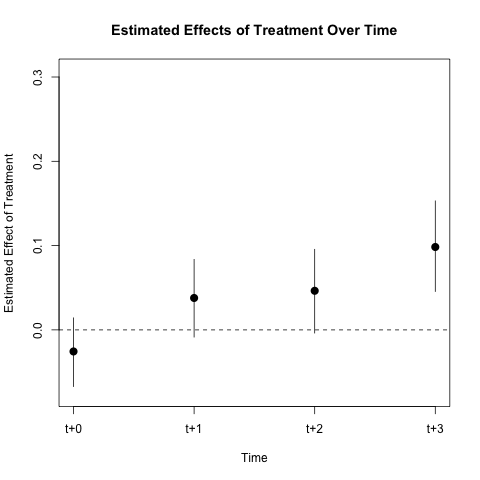
\includegraphics[width=0.75\textwidth]{Chapter1/Figures/panelmatch_logdefuncionespc.png}
       \captionsetup{justification=centering}
    
        
 \textbf{Note:} Figure \ref{fig:matching_violence} produced by propensity score matching that adjust for the treatment and covariate histories during the 5 year periods prior to the treatment. I report 95\% bootstrap confidence intervals clustered at the state level. Covariates include those used to generate Figure \ref{fig:event_study_agreements}. 
 
\end{figure}   
           
    
    
 \clearpage   
 
 %%%% NO ANTICIPATORY ASSUMPTION   
\section{Validating the no-anticipatory assumption \label{appendix:CDLZ}}

%\renewcommand{\thetable}{C-\arabic{table}}
%\setcounter{table}{0}
% \renewcommand{\thefigure}{C-\arabic{figure}}
%\setcounter{figure}{0}
    
         
One way to address the no-anticipatory behavior is to assume that it can only occur in a fixed window prior to the electoral reform, say of one year, especially since the reform was announced in early 2013. However, for states that implemented reelection later this fixed window assumption would not suffice. In other words, only those early adopters of the reform would show unbiased estimates. Late adopters, however, would anticipate the term limit removal an act accordingly biasing the results upwardly.  
 
Another way to assess the no-anticipatory behavior from incumbents in this setting is test whether early vs late adopters differed in their estimated effects. Appendix Figure \ref{fig:CDLZ_agreements} presents \citet{cengiz_etal_2019} ``event-by-event analysis" that estimates treatment effects for each treated Mexican state (28 states) in the sample. States color differs if they are early (2015, red color) or late adopters (2016-2018, blue color). Specifically, I create state-event specific panel datasets and estimate state-specific estimates using separate regressions for each state. Each state dataset contains the treated state and all other states that never received treatment or received treatment after the sample window of $t+1$. For each state I estimate the following DiD regression: 
   
\begin{equation}
y_{mt}=\mu_m	 + \mu_t + \gamma Reform_{mt} + \epsilon_{mt}
\end{equation}

where $Reform_{mt}$ is an indicator variable that takes the value of 1 if the state implemented reelection. If there was evidence of strong incumbent anticipatory behavior, conditional on state covariates such as governor winning margin and alignment with Federal Executive, we would expect strong color clustering across similar estimated effects. In other words, if there is an endogenous response by states to implement the electoral reform, we would see that the positive (or negative) treatment effect would be only by those that implemented reelection earlier or later (events with the same color would be clustered). However, as seen in Appendix Figure \ref{fig:CDLZ_agreements}, this is not the case: there is wide variation in estimated coefficients across early (red) and late (blue) adopters of the reform, conditional and unconditional on state covariates. One would be concerned of the five blue states clustered in the positive end. However, if there was anticipation in these states they would only represent a downward bias of the main results found on the paper.  

\begin{figure}[h]
\centering
\caption{``Event-by-event analysis'' following \citet{cengiz_etal_2019}\\ -95\% confidence intervals-} 
\label{fig:CDLZ_agreements}
\includegraphics[width=0.5\textwidth]{Chapter1/Figures/CDLZ_cov_acuerdo.png}
       \captionsetup{justification=centering}
       \\
 {\textbf Note:} Estimate separate treatment effects for each event, i.e. each Mexican state in the sample. Each event dataset contains the treated state and all other states that never received treatment or received treatment after the sample window ($t+1$).   
\end{figure}     
   
For robustness, Appendix Figure \ref{fig:stacked_wcontrols_agreements} presents the ``stacked dataset analysis" from \citet{cengiz_etal_2019}. I take each of the ``event-by-event'' datasets from the Appendix Figure \ref{fig:CDLZ_agreements}, stack estimates by cohort and estimate one set of lead and lag variables not using prior treated units as controls. Appendix Figure \ref{fig:stacked_wcontrols_agreements} shows that conditional on state-level covariates, there is strong evidence of parallel trends as well as negative effect of reelection on delegation, but noisy.
       
    
\begin{figure}[H]
\centering
\caption{``Stacked dataset analysis'' following \citet{cengiz_etal_2019}\\ -95\% confidence intervals-} 
\label{fig:stacked_wcontrols_agreements}

\includegraphics[width=0.5\textwidth]{Chapter1/Figures/stacked_dataset_wcontrols_acuerdo.png}
       \captionsetup{justification=centering}
       \\
 {\textbf Note: Utilize estimated coefficients from Figure \ref{fig:CDLZ_agreements} and stack them in relative time, and estimate lead and lag variables to treatment following the event-by-event analysis setup, i.e. without treatment containment from using prior treated units of controls. Analysis done stacking at the cohort level, and adding municipality and year fixed effects, and clustered standard errors at the state level.}     
\end{figure}   


\chapter{Appendix of ``Love the Candidate but Hate his Party: The Asymmetric Effects of Reelection Incentives on Partisan and Personal Incumbency Returns in Mexico'' \label{chap:append2}}

\break

%\section{Tables and Figures}

\begin{table}[H]
\centering 
\caption{Descriptive statistics}
   
\label{tab:descriptive}
\scalebox{0.55}{ 
{
\def\sym#1{\ifmmode^{#1}\else\(^{#1}\)\fi}
\begin{tabular}{l*{1}{ccccc}}
\hline\hline
            &        \textbf{Mean}&  \textbf{SD}&  \textbf{Min}&  \textbf{Max}& \textbf{N}\\
\hline    
\emph{Pane A - Incumbency Advantage:} 	&		&		&		&		\\
Probability of winning, election at t+1&        0.40&        0.49&           0&           1&       2,247\\
Vote share, election at t+1&       -0.05&        0.18&          -1&         .59&       2,246\\

\\
\emph{Panel B - Treatments and Forcing Variable:} 	&		&		&		&		\\
Term Limit Removed=1; 0 otherwise&        0.29&        0.45&           0&           1&       2,247\\
Win election at t=1; 0 otherwise&        0.46&        0.50&           0&           1&       2,247\\

Winning margin: first - second runner&        0.07&        0.05&        0.00&        0.33&       2,247\\


\\
\emph{Panel C - Pretreatment controls:} 	&		&		&		&		\\
Winning margin: first - second runner (governor)&        0.15&        0.13&           0&           1&      24,470\\
Party alignment with federal executive=1; 0 otherwise&        0.54&        0.50&           0&           1&      24,470\\

Population (INEGI and CONAPO projections)&      49,233&     129,415&         409&   1,714,709&       2,247\\


\\
\emph{Panel D - Mechanisms-Fiscal Transfers:} 	&		&		&		&		\\
General Participations Fund (Mill. pesos)&          39&          94&         .81&       1,221&       1,638\\
Participating Fund (Mill. pesos)&          52&         127&         .21&       1,498&       1,656\\
Municipal Development Fund (Mill. pesos)&         9.7&          24&          .2&         345&       1,642\\
Federal and state contributions (Mill. pesos)&          60&         131&        .048&       2,133&       1,768\\
Contribution Fund for Municipal Social Infrastructure (Mill. pesos)&          18&          30&        .048&         618&       1,759\\
Contribution Fund to Strengthen Municipalities (Mill. pesos)&          23&          61&         .15&         865&       1,755\\

\\
\emph{Panel E - Mechanisms-Municipal Revenues:} 	&		&		&		&		\\
Total Municipal Revenues (Mill. pesos)&         166&         420&           2&       5,715&       1,779\\
Tax Revenues (Mill. pesos)&          19&          82&      .00017&       1,256&       1,735\\
Property Tax Rrevenues (Mill. pesos)&          12&          48&      .00013&         476&       1,360\\
Estate Tax Revenues (Mill. pesos)&          17&          66&      .00013&         672&       1,506\\
Prod., Cons. and Trans. Tax Revenues (Mill. pesos)&         1.2&          19&     .000096&         488&         671\\
Vehicle Ownership Tax Revenues (Mill. pesos)&          .5&         1.9&     .000081&          29&       1,324\\
New Cars Tax Revenues (Mill. pesos)&         .87&         2.9&       .0032&          49&       1,530\\
Public Security Revenues (Mill. pesos)&         6.1&          15&     .000078&         121&         211\\

\\
\emph{Panel F - Mechanisms-Other Resources:} 	&		&		&		&		\\
Number of City Council Sessions&          23&          19&           0&         288&       1,784\\
Number of Approved Initiatives of Law&          17&          32&           0&         295&         884\\
Percentage of Municipal Budget Spend&          11&          15&           0&         100&         789\\
Bureaucrats per 100,000 inhabitants&       1,945&       2,601&           0&      24,528&       1,247\\

\\
\emph{Panel G - Mechanisms-Incumbents' quality:} 	&		&		&		&		\\
Incumbent undergraduate or graduate title (indicator)&        0.06&        0.24&           0&           1&      19,430\\

\\ 

\hline\hline
\end{tabular}    
}
}
\end{table} 
   


 \begin{figure}[h]   
\centering
 \caption{No discontinuous jump of covariates}
 \label{fig:jump_covariates}
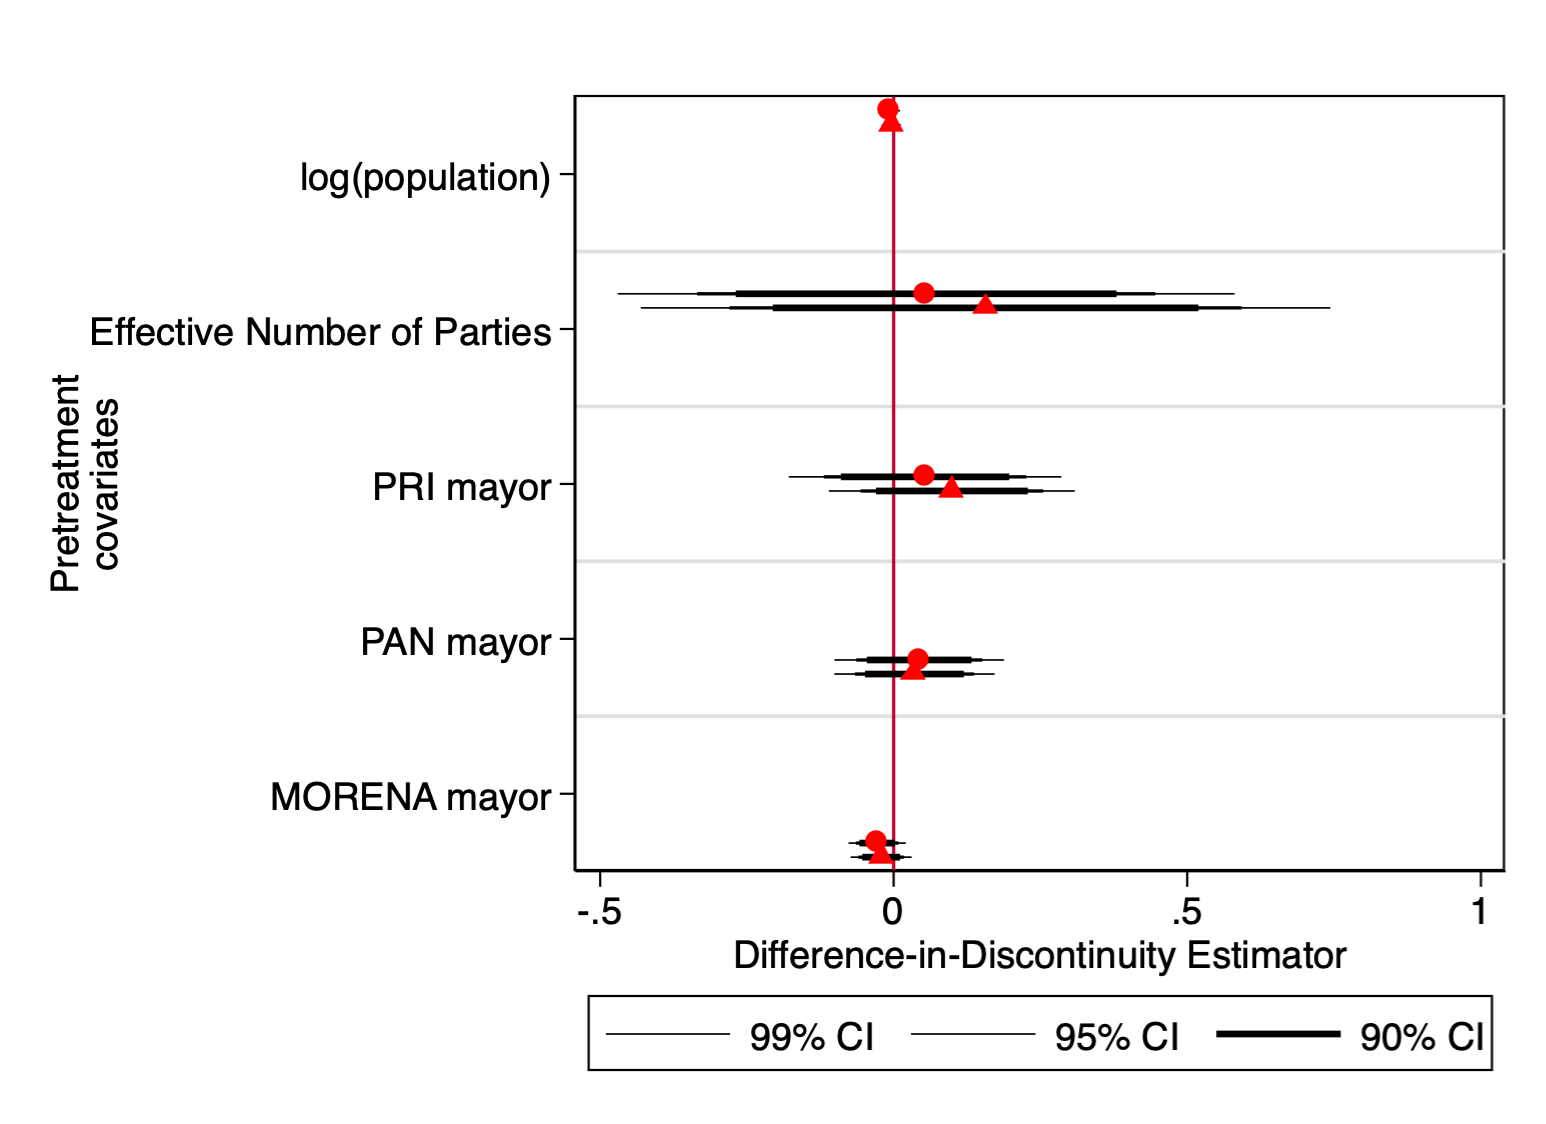
\includegraphics[width=0.9\textwidth]{Chapter2/Figures_incumbency/nojump.png}
       \captionsetup{justification=centering}
    
 \textbf{Note:} Figure \ref{fig:jump_covariates} shows the average treatment effect of the Term Limit Reform on various pretreatment covariates using a difference in discontinuity of close elections design. Optimal bandwidths following \citet{calonicoetal_2014} are used. 
   
\end{figure} 

  
    
    
\begin{figure}[h]   
\centering
 \caption{McCrary Test}
 \label{fig:mccrary}
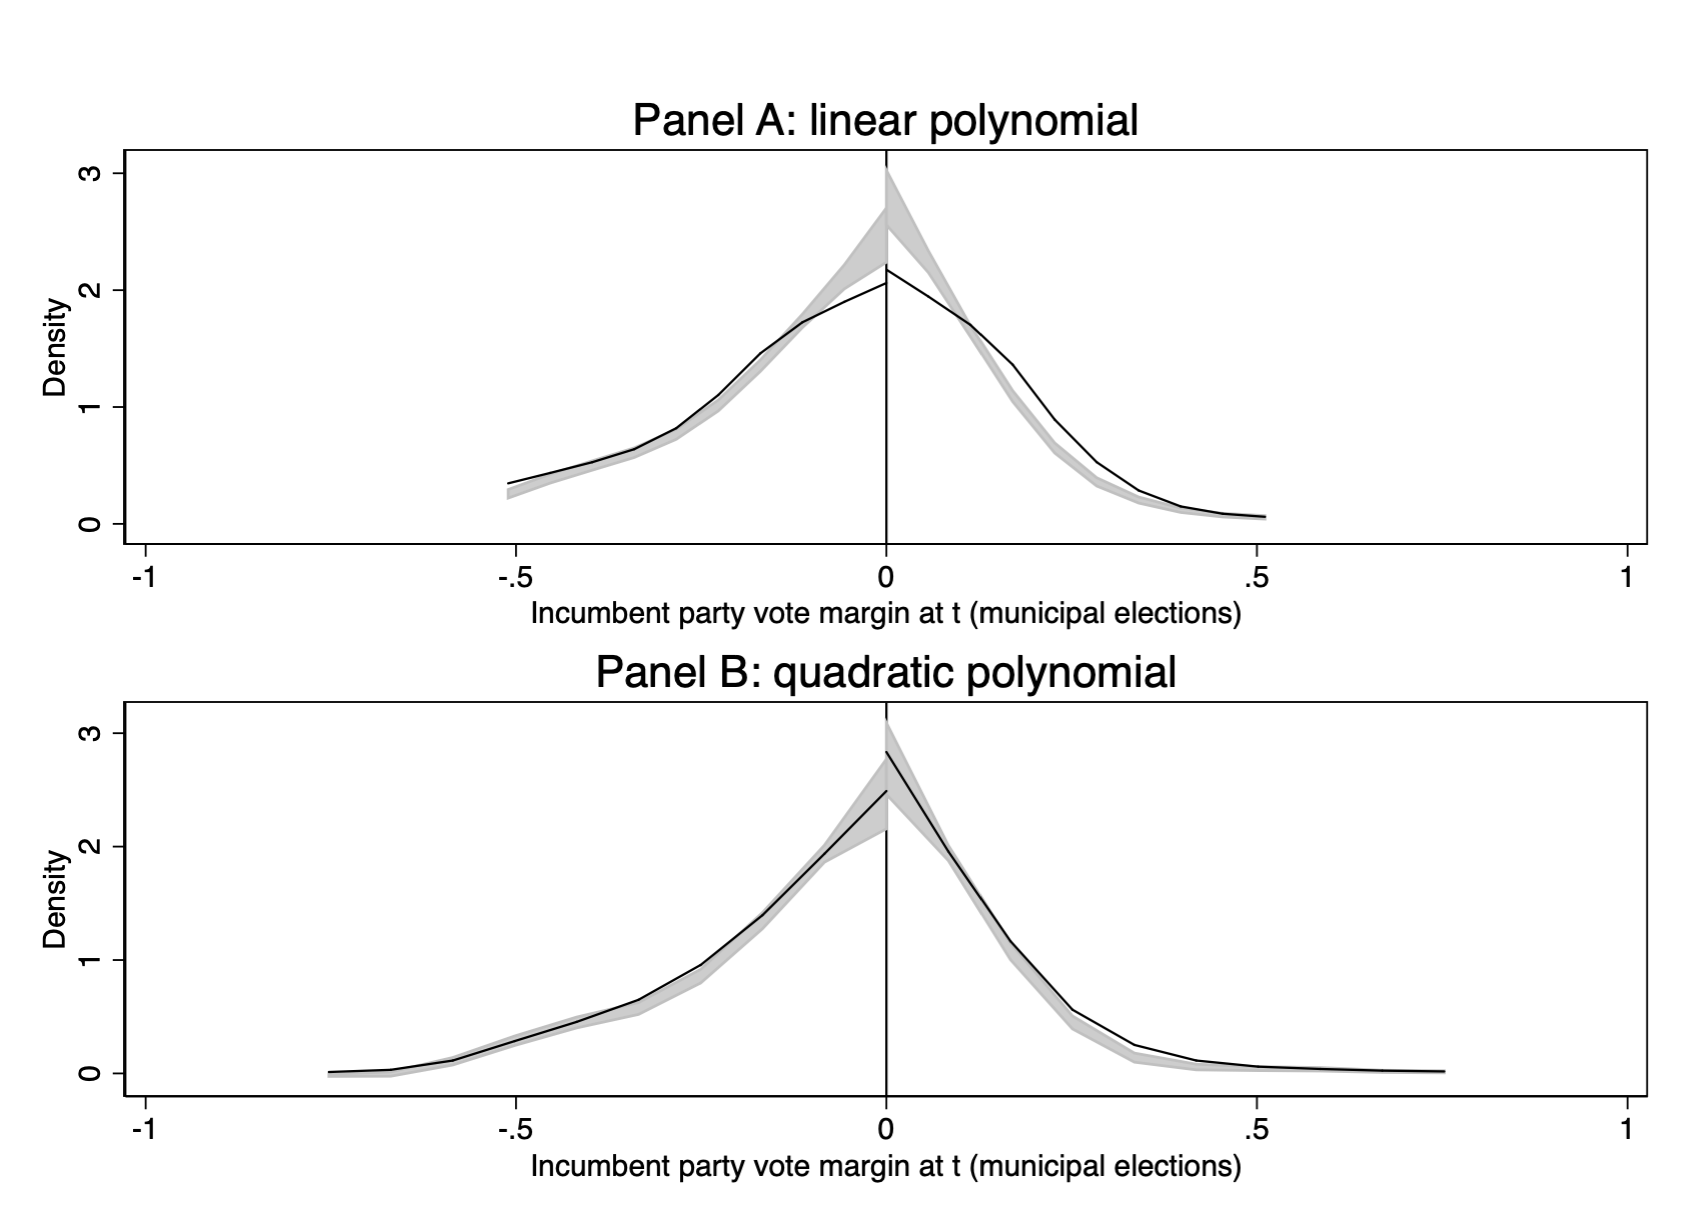
\includegraphics[width=1\textwidth]{Chapter2/Figures_incumbency/mccrary_pol1_2.png}
%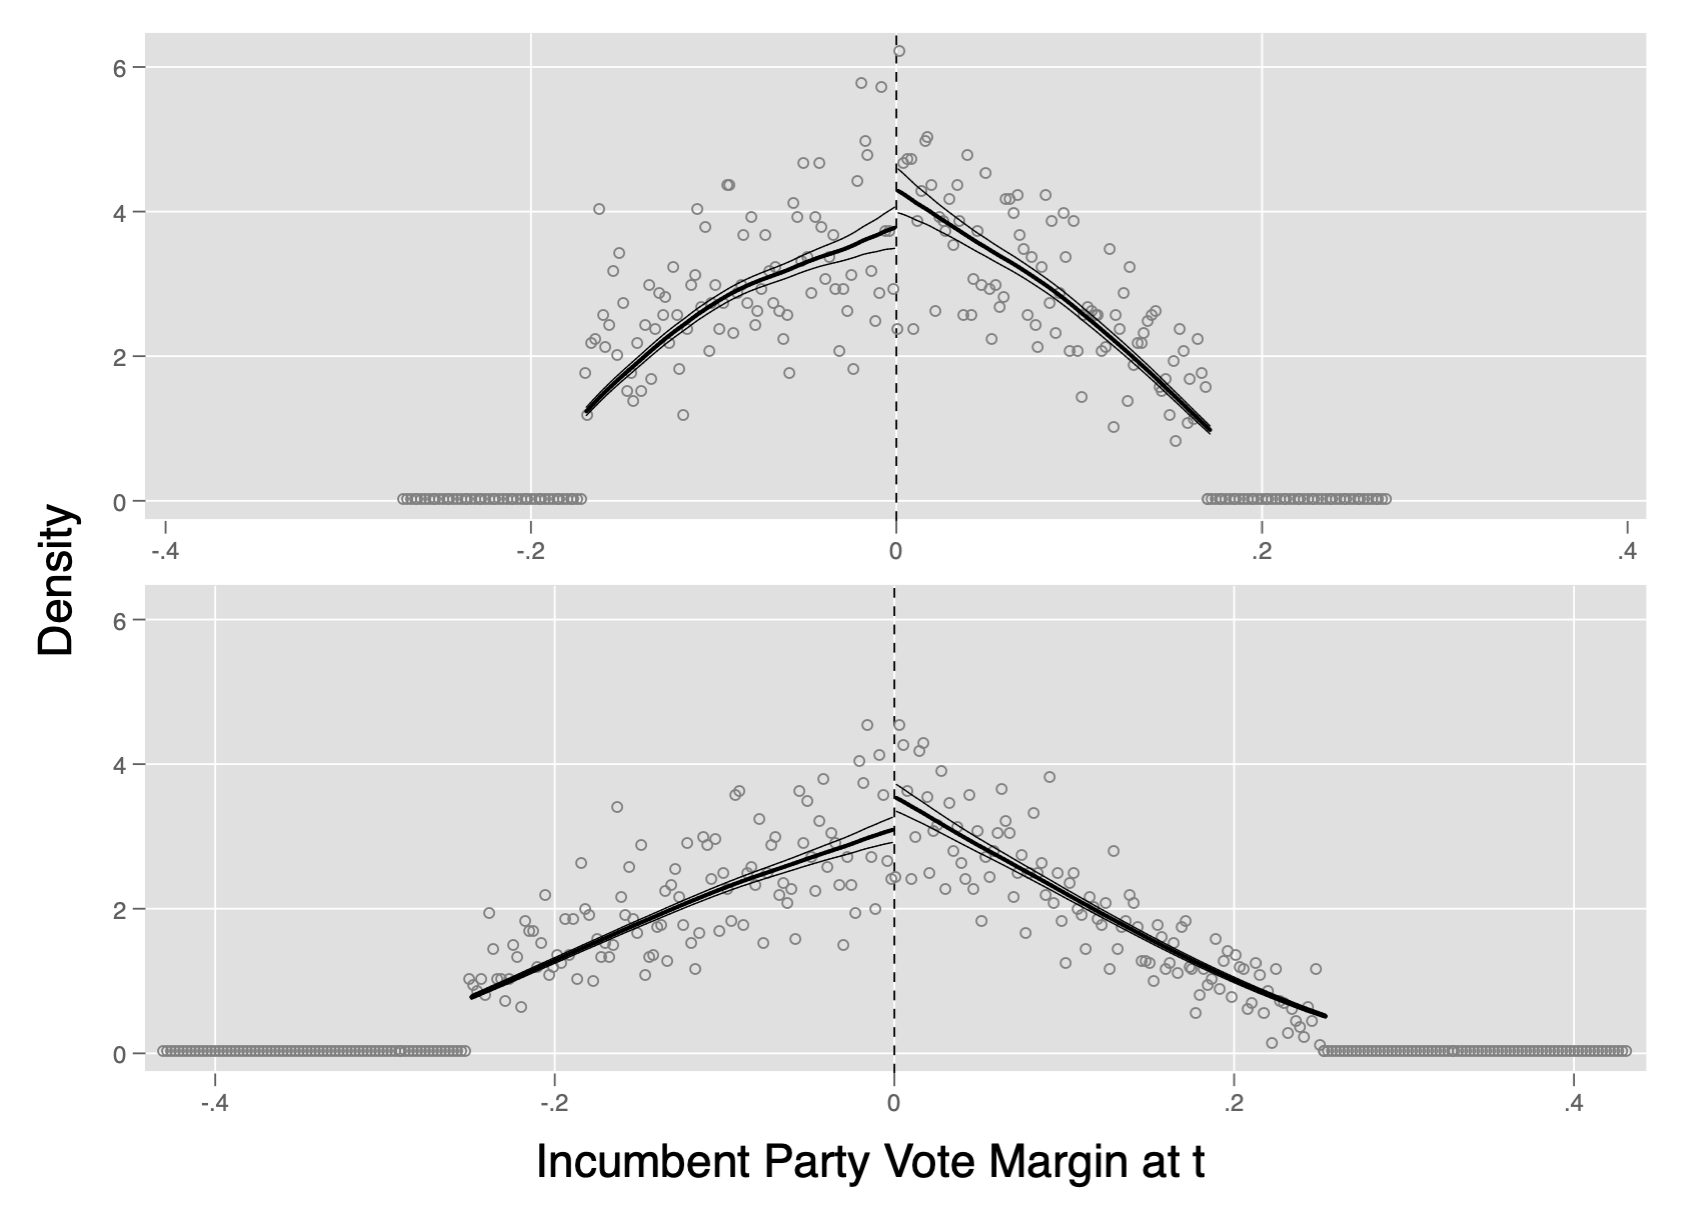
\includegraphics[width=0.9\textwidth]{../Figures/conditional_mccrary_test_pol1_final.png}

       \captionsetup{justification=centering}
         
 \textbf{Note:} 95\% confidence intervals reported.
 
\end{figure} 


 \begin{figure}[h]   
\centering
 \caption{Testing Different Bandwidths}
 \label{fig:bandwidths}
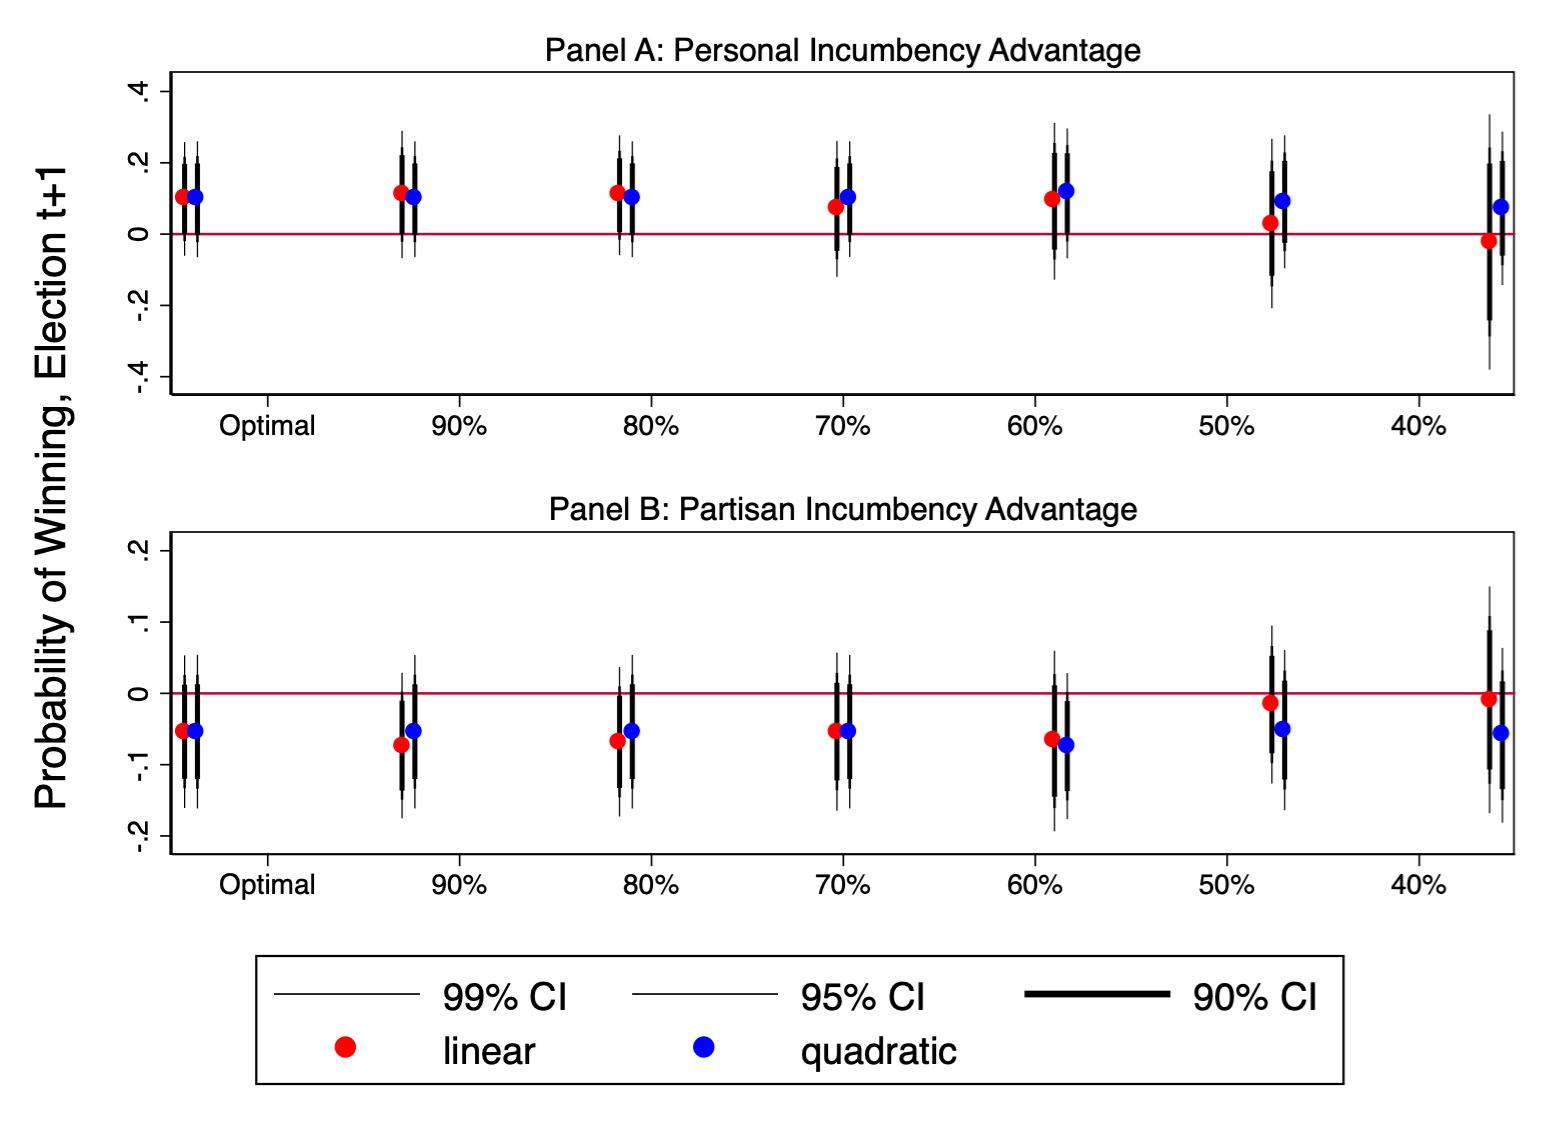
\includegraphics[width=0.65\textwidth]{Chapter2/Figures_incumbency/probability_bandwidths.png}
       \captionsetup{justification=centering}
 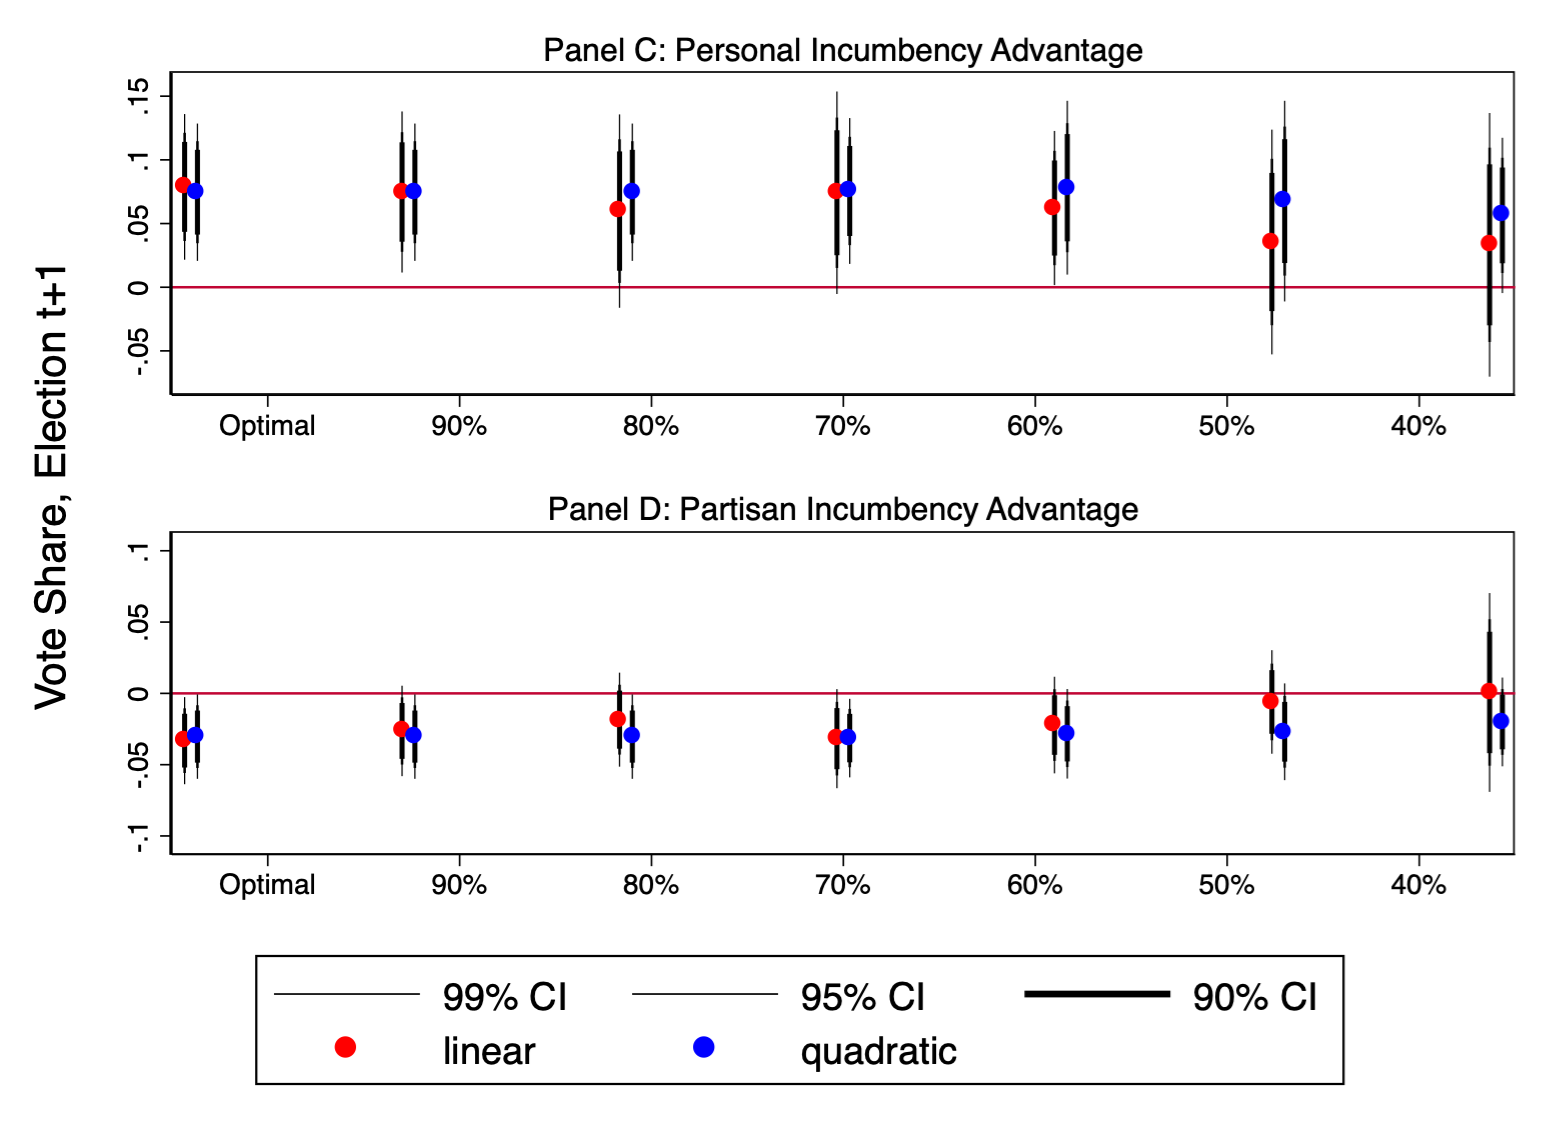
\includegraphics[width=0.65\textwidth]{Chapter2/Figures_incumbency/margin_bandwidths.png}

 \textbf{Note:} Figure \ref{fig:bandwidths} shows the average treatment effect of the Term Limit Reform on the probability of victory in the next election. Various bandwidths are tested as well as the optimal bandwidth following \citet{calonicoetal_2014}. A 90\% implies a reduction of the optimal bandwidth in 10\%, an 80\% a reduction of 20\%, and so on.
   
\end{figure} 
  
\chapter{Appendix of ``Endogenous taxation in ongoing internal conflict: The case of Colombia'' \label{chap:append3}}

%%----------------------------------------%%
\section{Data \label{data_appendix3}}

\subsection{Tax Revenue and Institutions \label{appendix3:taxrevenues&institutions}}

Our data on local tax revenue come from the National Planning Department (Departamento Nacional de Planeaci\'{o}n (DNP)), which compiles the data from the municipalities. Municipal authorities submit a quarterly form called the ``Unique Tributary Form'' (Formato \'Unico Tributario (FUT)), which is sent to the Ministry of Finance. The DNP processes the information as annual averages with a roughly 4-year lag. As noted above, the primary source of local tax revenue is the property tax. We estimate the logged average of local tax revenues at the municipal level for each of the time periods that characterize the Colombian civil war since the 1980s (subsection on ``Civil War and Capture in Colombia''). 

To measure other aspects of tax institutions, we constructed four variables using publicly available data from IGAC, the national land registry service: the per capita land value, the number of land registry updates, the time elapsed since the last registry update, and the land informality rate per municipality. 

\subsection{Violence \label{appendix3:violence}}

Our main explanatory variables are violence by guerillas and paramilitary groups at the municipal level. As noted in $H_1a$ above, we expect that violence perpetrated by the FARC is likely to have a  negative impact on tax collection and formality. In contrast, as noted in $H_2a$, paramilitary activity is expected to be associated with formalization in favor of their landholding supporters and therefore greater net tax receipts.

Our data on violence at the municipal level was compiled by \citet{restrepoetal03}, and updated by Universidad el Rosario through 2014. The data record for every event its location and date, its perpetrator and type (distinguishing between unilateral bellicose activities like guerrilla attacks, and combats between two of the conflict parties), and the resulting casualties. To assess net influence in a given time period, we aggregated all attacks by armed groups of a certain type over the periods described in the subsection on ``Civil War and Capture in Colombia'', normalize for population, and log the resulting cumulative variable given the existent skewness. Note that this monotonic transformation effectively reduces the weights of outliers in the specification as a way for correcting for such.

\subsection{Electoral outcomes \label{appendix3:electoral_outcomes}}

Electoral data on all local elections from 1997 to 2011 was compiled by \citet{pachonsanchez14}, suing as a primary source the reports of {\it Registradur\'ia Nacional del Estado Civil}, Colombia's electoral and identity bureau. Both mayor and city councils were elected in 1997, 2000, 2003, 2007 and 2011. Elected officials had three-year terms until 2003, when terms extended to four years.

Because right wing parties had clear tax policy preferences we measure political alignment with a dummy variable equal to 1 if the elected mayor belong to the President's Uribe 2000s political party coalition, 0 otherwise. The coalition included the Conservative Colombian party and the following right- or center-right-wing parties: Cambio Radical, Partido Social de Unidad Nacional (Partido de la U), Colombia Democr\'atica, Convegencia Ciudadana and Alas Equipo Colombia.

\subsection{Social outcomes and economic activity \label{appendix3:social_outcomes}}

Municipal governments in Colombia provide a series of social outcomes through public good services, and thus are subject to potential effects by armed groups, through a capture of local authorities (see Appendix \label{appendix3:test_electoral_mechanism}). 

We rely on social outcomes from DANE such as secondary enrollment and measures of quality of education through math scores of standardized national tests (SABER 11).  

Lastly, to measure economic activity at the municipal level over the period from 1997 to 2013, we rely on nighttime light data. Specifically, we use version 4 of the data collected by the Defense Meteorological Satellite Program (DMSP-OLS), and available through the National Oceanic and Atmospheric Administration's (NOAA) National Center for Environmental Information (NECI).\footnote{The DMSP satellites take images with a resolution of 30 arc-seconds (roughly 1 square km at the equator). The imagery removes snow, clouds, fires, gas flares and other ephemeral lights. Each 30 arc-second pixel has a 0 to 63 digital number assigned according to its luminosity intensity. However, due to problems related to degradation of the sensors, satellites trajectory and scanning procedure, and the differences in crossing time between satellites, the data suffers from a series of problems that affects it comparability across time. These include: discrepancies in the digital number among satellites from the same year; abrupt abnormal fluctuations in digital number values for different years, for the same satellite; substantial differences in the number of lit pixels for satellite at the same year; geographic misalignment; and, most importantly, blurring due to light over glow across space, which increases as the digital number grows, and thus biases more luminous areas (Baugh et al. 2010; Elvidge et al, 2009; Liu et al, 2012; Zhang \& Seto, 2011). Thus, to assure comparability across time and between satellites we intercalibrated the data following Wu et al. (2013), perform a geometric correction following  Zhao et al. (2015), and estimate an intra-annual composition for the cases where two satellites captured light for the same time period. Pixels who appeared in one of the satellites but not the other where labeled as unstable lit pixels and turned into missing values. The remaining stable lit pixels' digital numbers where averaged, a process which produced one intra-annual composite by year.}   Luminosity data recorded by satellites have been shown to be a consistent predictor of economic activity at both national and sub-national levels \citep{vernon11, bleakley2012, michalopoulos2013, storeygard2012, pinkosalai2014}, and have even been used for border-specific economic performance comparisons across very short geographical spaces \citep{pinko2013}. Recent work using geo-located Demographic and Health Survey (DHS) data confirm that luminosity tracks well with sub-national measures of economic activity in a range of developing world settings \citep{weidmann2017}.

\subsection{Other variables \label{appendix3:other_vars}}

Our dataset also contains a number of important controls including other fiscal measures  (such as transfers from the central government and royalties from the exploitation of natural resources), geographical characteristics of municipalities related to state presence and economic isolation such as the distance to the department's capital, pre-period vote share by political party ideology which is particularly important when measuring the effect of presence of armed groups on electoral outcomes, a dummy variable on whether a municipality had no registered homicides in the same period as the cumulative attack variable (to avoid a selection bias on armed group presence), the number of military bases in each time period from 1999 to 2009 to account for extra-normal state presence, and the number of people displaced, driven out, and received  by municipality due to conflict, which is important when assessing electoral outcomes. We also include an additive endowment index on the municipality production of gold, silver, platinum, nickel, emeralds and iron. Coca production levels are also included given the rapacity effect that this illegal market may generate on both armed groups' behavior.  

Table \ref{appendix3:descriptive} reports the descriptive statistics of all the variables (except the main variables, described in Table \ref{chapter3_tab:descriptive}). In turn, Table \ref{appendix3:description_vars} provides further details on the variables' sources.

%%-----------------------------------------------------------%
%Table 1A

\begin{table}[h]\centering \caption{Descriptive statistics of additional variables}
\label{appendix3:descriptive}
\scalebox{0.6}{
\begin{tabular}{l c c c c c}\hline\hline
\multicolumn{1}{c}{\textbf{Variable}} & \textbf{Mean}
 & \textbf{Std. Dev.}& \textbf{Min.} &  \textbf{Max.} & \textbf{N}\\ \hline
 \\
\multicolumn{6}{c}{Panel A. Outcomes }\\ 
 
{\it Social outcomes}	&		&		&		&		&		\\ 

Secondary enrollment rate 2003-2006&        0.60&        0.22&           0&           2&        1128\\
Quality of education (average math score) 2003-2006&       -0.16&        0.16&          -1&           1&         972\\



\\
{\it Economic activity}	&		&		&		&		&		\\ 

Log luminosity per capita 1997-2002&       -8.42&        1.11&         -12&          -4&        1063\\
Log luminosity per capita 2003-2006&       -8.52&        1.10&         -12&          -4&        1063\\
Log luminosity per capita 2007-2010&       -8.27&        1.15&         -12&          -4&        1063\\
Log luminosity per capita 2011-2013&       -8.33&        1.18&         -13&          -4&        1063\\


\\
{\it Vote share by political party coalition (Mayor elections)
}	&		&		&		&		&		\\ 

Uribe + Conservative party coalition 1997 and 2000 Mayor elections&        0.26&        0.32&           0&           1&        1020\\
Uribe + Conservative party coalition 2003 Mayor election&        0.22&        0.26&           0&           1&         914\\
Uribe + Conservative party coalition 2007 Mayor election&        0.58&        0.31&           0&           1&        1112\\
Uribe + Conservative party coalition 2003 and 2007 Mayor elections&        0.43&        0.26&           0&           1&        1114\\
Uribe + Conservative party coalition 2011 Mayor election&        0.41&        0.33&           0&           1&        1046\\



\\
{\it Vote share by political party coalition (City Council elections)
}	&		&		&		&		&		\\ 

Uribe + Conservative party coalition 1997 and 2000 City Council elections&        0.28&        0.24&           0&           1&        1101\\
Uribe + Conservative party coalition 2003 and 2007 City Council elections&        0.42&        0.18&           0&           1&        1114\\
Uribe + Conservative party coalition 2011 City Council election&        0.37&        0.20&           0&           1&        1046\\


\\
\multicolumn{6}{c}{Panel B. Violence}\\
{\it Violence (no-logs; with Table \ref{chapter3_tab:main} third period specification sample)}	&		&		&		&		&		\\ 

Guerrilla attacks per 100,000 inh. 1988-1996&       62.67&      118.76&           0&        1260&        1182\\
Paramilitary attacks per 100,000 inh. 1988-1996&       36.31&       74.22&           0&        1742&        1182\\
Guerrilla attacks per 100,000 inh. 1997-2002&       76.32&      128.62&           0&        1734&        1182\\
Paramilitary attacks per 100,000 inh. 1997-2002&       38.08&       56.12&           0&         581&        1182\\
Guerrilla attacks per 100,000 inh. 2003-2006&      116.18&      283.43&           0&        3372&        1182\\
Paramilitary attacks per 100,000 inh. 2003-2006&       30.01&       59.28&           0&         672&        1182\\
Guerrilla attacks per 100,000 inh. 2007-2010&       73.51&      169.31&           0&        1873&        1182\\
Paramilitary attacks per 100,000 inh. 2007-2010&       32.31&       60.71&           0&         672&        1182\\



\\

{\it Violence distribution moments (to compute marginal effects)} & \textbf{Median} & \textbf{p(90)}&  &   & \\
 Guerrilla attacks per 100,000 inh. 1988-1996&       17.44&      185.90\\
Paramilitary attacks per 100,000 inh. 1988-1996&       20.44&       94.55\\
Guerrilla attacks per 100,000 inh. 1997-2002&       35.83&      211.92\\
Paramilitary attacks per 100,000 inh. 1997-2002&       22.50&      102.23\\
Guerrilla attacks per 100,000 inh. 2003-2006&       24.57&      308.50\\
Paramilitary attacks per 100,000 inh. 2003-2006&       12.30&       83.92\\
Guerrilla attacks per 100,000 inh. 2007-2010&       16.81&      210.98\\
Paramilitary attacks per 100,000 inh. 2007-2010&       14.04&       89.45\\

 
  Guerrilla attacks per 100,000 inh. 2003-2010 \footnote{Using Table 6, panel A, third period specification sample.}&       53.16&      461.66\\
Paramilitary attacks per 100,000 inh. 2003-2010 \footnote{\emph{Same as last footnote.}}&       14.35&       89.49\\



\\

\multicolumn{6}{c}{Panel C. Controls}\\
{\it Vote share by political party ideology (Mayor elections)
}	&		&		&		&		&		\\ 

Left-wing party 1994&        0.02&        0.13&           0&           1&        1182\\
Traditional party 1994&        0.73&        0.44&           0&           1&        1182\\
Third (right-wing) party 1994&        0.24&        0.43&           0&           1&        1182\\
Indigenous Afro-Colombian party 1994&        0.01&        0.09&           0&           1&        1182\\
Left-wing party 2000&        0.01&        0.08&           0&           1&        1182\\
Traditional party 2000&        0.51&        0.50&           0&           1&        1182\\
Third (right-wing) party 2000&        0.47&        0.50&           0&           1&        1182\\
Indegenous Afro-Colombian party 2000&        0.01&        0.11&           0&           1&        1182\\
Left-wing party 2007&        0.02&        0.12&           0&           1&        1182\\
Traditional party 2007&        0.31&        0.46&           0&           1&        1182\\
Third (right-wing) party 2007&        0.63&        0.48&           0&           1&        1182\\
Indigenous Afro-Colombian party 2007&        0.04&        0.20&           0&           1&        1182\\
Left-wing party 2011&        0.01&        0.08&           0&           1&        1182\\
Traditional party 2011&        0.28&        0.45&           0&           1&        1182\\
Third (right-wing) party 2011&        0.67&        0.47&           0&           1&        1182\\
Indigenous Afro-Colombian party 2011&        0.04&        0.20&           0&           1&        1182\\

\hline
\end{tabular}
}
\end{table}


% Table 1. Descriptive stats - Continue

%-----------------------------------------------------------%
\begin{table}[h]\centering \caption{Descriptive statistics of additional variables (continuation)}
\label{appendix3:descriptive_2}
\scalebox{0.6}{
\begin{tabular}{l c c c c c}\hline\hline
\multicolumn{1}{c}{\textbf{Variable}} & \textbf{Mean}
 & \textbf{Std. Dev.}& \textbf{Min.} &  \textbf{Max.} & \textbf{N}\\ \hline
\\
{\it Population (not used as a control)}	&		&		&		&		&		\\ 

Log (mean) population 1988-1996&        9.49&        1.05&           5&          15&        1088\\
Log (mean) population 1997-2002&        9.50&        1.08&           5&          16&        1128\\
Log (mean) population 2003-2006&        9.52&        1.10&           5&          16&        1128\\
Log (mean) population 2007-2010&        9.54&        1.12&           6&          16&        1132\\
Log (mean) population 2011-2013&        9.55&        1.14&           6&          16&        1132\\


\\

{\it Federal Government Windfall}	&		&		&		&		&		\\ 

Royalties per capita  1988-1996&        0.00&        0.01&           0&           0&        1071\\
Royalties per capita  1997-2002&        0.03&        0.12&           0&           2&        1108\\
Royalties per capita  2003-2006&        0.04&        0.24&           0&           6&        1107\\
Royalties per capita  2007-2010&        0.06&        0.28&           0&           4&        1111\\
Transfers per capita 1988-1996&        0.11&        0.09&           0&           2&        1071\\
Transfers per capita 1997-2002&        0.05&        0.05&           0&           1&        1108\\
Transfers per capita 2003-2006&        0.06&        0.07&           0&           2&        1107\\
Transfers per capita 2007-2010&        0.07&        0.10&           0&           2&        1111\\




\\
{\it Military bases}	&		&		&		&		&		\\ 

Military bases 1999-2002&      328.08&      171.84&           0&        1309&        1132\\
Military bases 2003-2006&      177.67&       96.07&           0&         878&        1132\\
Military bases 2007-2009&      160.68&       90.82&           0&         761&        1132\\



\\
{\it Peaceful municipalities}	&		&		&		&		&		\\ 

Peaceful Municipalities (no attacks) 1988-1996&        0.27&        0.44&           0&           1&        1182\\
Peaceful Municipalities (no attacks) 1997-2002&        0.16&        0.37&           0&           1&        1182\\
Peaceful Municipalities (no attacks)2003-2006&        0.20&        0.40&           0&           1&        1182\\
Peaceful Municipalities (no attacks)2007-2010&        0.34&        0.47&           0&           1&        1182\\



\\
{\it Displacements}	&		&		&		&		&		\\ 

Desplazados received 1997-2002&     1247.29&     4982.80&           0&       71649&        1182\\
Desplazados received 2003-2006&      882.65&     4015.96&           0&       98005&        1182\\
Desplazados received 2007-2010&      529.79&     3270.09&           0&       79541&        1182\\
Desplazados driven out 1997-2002&     1224.65&     3581.72&           0&       46593&        1182\\
Desplazados driven out 2003-2006&      912.16&     1995.68&           0&       28149&        1182\\
Desplazados driven out 2007-2010&      540.38&     1456.78&           0&       22351&        1182\\
Desplazados 1997-2002&      958.80&     2563.65&           0&       39860&        1182\\
Desplazados 2003-2006&      891.31&     1996.23&           0&       29047&        1182\\
Desplazados 2007-2010&      668.05&     1838.26&           0&       28327&        1182\\



\\
{\it Cocaine production}	&		&		&		&		&		\\ 

Cocaine production (cum. tons) 1993-1996&        0.00&        0.00&           0&           0&        1182\\
Cocaine production (cum. tons) 1997-2002&      514.49&     3327.72&           0&       46762&        1182\\
Cocaine production (cum. tons) 2003-2006&      283.06&     1545.78&           0&       21456&        1182\\
Cocaine production (cum. tons) 2007-2010&      264.31&     1262.36&           0&       21653&        1182\\
Cocaine production (cum. tons) 2003-2010&      547.37&     2734.69&           0&       42825&        1182\\




\\
{\it Endowments}	&		&		&		&		&		\\ 

Endowments (additive index; cum. tons)\footnote{Includes gold, silver, platinum, nickel, emeralds and oil.} 1999-2002& 32393338.95&    2.68e+08&           0&    5.42e+09&        1128\\
Endowments (additive index; cum. tons) 2003-2006& 70961196.19&    7.31e+08&          -0&    2.11e+10&        1128\\
Endowments (additive index; cum. tons) 2007-2010&    1.00e+08&    7.74e+08&           0&    1.90e+10&        1132\\
Endowments (additive index; cum. tons) 2003-2010& 85598159.61&    7.40e+08&          -0&    2.00e+10&        1132\\



\\
{\it Geography}	&		&		&		&		&		\\ 

Municipal area      &     1000.66&     3155.40&           0&       65674&        1132\\
Elevation           &     1127.63&      921.82&           0&        3350&        1132\\
Distance to the Department's capital&      122.83&      106.15&           0&         790&        1125\\


\hline \hline
\end{tabular}
}
\end{table}

%--------------------------------------
%Table 2A: Variables, Description and Sources
\begin{landscape}
\begin{table}[]
\centering
\caption{Variables, Description and Sources}
\label{appendix3:description_vars}
\scalebox{0.6}{
\begin{tabular}{lll}
\hline
\multicolumn{1}{c}{\textbf{Variable}} & \multicolumn{1}{c}{\textbf{Description}} & \multicolumn{1}{c}{\textbf{Source}} \\ \hline
\begin{tabular}[c]{@{}l@{}}Time periods for \\ dependent variables, \\ independent variables, \\ and controls: *\end{tabular} & \multicolumn{1}{c}{1997-2002; 2003-2006; 2007-2010; 2011-2013} &  \\
\begin{tabular}[c]{@{}l@{}}Time periods for \\ dependent variables, independent \\ variables, and controls: **\end{tabular} & \multicolumn{1}{c}{1988-1996; 1997-2002; 2003-2006; 2007-2010} &  \\
\begin{tabular}[c]{@{}l@{}}Time periods for \\ dependent variables: ***\end{tabular} & \multicolumn{1}{c}{1994, 1997, 2000, 2003, 2007, 2011} &  \\
\begin{tabular}[c]{@{}l@{}}Time period for \\ dependent variable:  +\end{tabular} & \multicolumn{1}{c}{2003-2006} &  \\
\begin{tabular}[c]{@{}l@{}}Time period of \\ control variable: ++\end{tabular} & \multicolumn{1}{c}{1994, 2000, 2003, 2007} &  \\
\begin{tabular}[c]{@{}l@{}}Timeless variables: \\ +++\end{tabular} & \multicolumn{1}{c}{.} &  \\
\multicolumn{3}{c}{\textbf{Panel A: Dependent variables}} \\
Property tax revenue* & \begin{tabular}[c]{@{}l@{}}Logged mean property tax revenue (over time period) in 2008 thousand \\ Colombian pesos.\end{tabular} & \begin{tabular}[c]{@{}l@{}}CEDE (Centro de Estudios sobre Desarrollo \\ Economico) Municipal Panel, Universidad \\ de Los Andes, Colombia\end{tabular} \\
\begin{tabular}[c]{@{}l@{}}Uribe coalition plus \\ conservative party \\ win dummy, Mayor \\ election***\end{tabular} & \begin{tabular}[c]{@{}l@{}}Dummy = 1 if Mayor (in a given municipality) from the Uribe coalition won; 0 \\ otherwise. The Uribe coalition plus the Conservative Party, is made up by Cambio \\ Radical, Partido Social de Unidad Nacional (Partido de la U), Partido Conservador \\ Colombiano, Colombia Democratica, Convergencia Ciudadana, and Alas equipo \\ Colombia.\end{tabular} & \begin{tabular}[c]{@{}l@{}}Colombia's National Registry data compiled \\ by Pachon and Sanchez (2014)\end{tabular} \\
\begin{tabular}[c]{@{}l@{}}Vote share for Uribe \\ coalition plus  \\ conservative party,  \\ Mayor election***\end{tabular} & \begin{tabular}[c]{@{}l@{}}Percentage of total votes for Mayor (in a given municipality) for all parties that \\ belong to the Uribe coalition plus the Conservative Party. The Uribe coalition plus \\ the Conservative Party, is made up by Cambio,Radical, Partido Social de Unidad \\ Nacional (Partido de la U), Partido,Conservador Colombiano, Colombia \\ Democratica, Convergencia Ciudadana,,and Alas equipo Colombia.\end{tabular} & \begin{tabular}[c]{@{}l@{}}Colombia's National Registry data compiled \\ by Pachon and Sanchez (2014)\end{tabular} \\
\begin{tabular}[c]{@{}l@{}}Vote share for Uribe \\ coalition plus \\ conservative party, \\ City Council \\ election***\end{tabular} & \begin{tabular}[c]{@{}l@{}}Percentage of total votes for City Council (in a given municipality) for all parties \\ that belong to the,Uribe coalition plus the Conservative Party. The Uribe \\ coalition plus,the Conservative Party, is made up by Cambio,Radical, \\ Partido Social de,Unidad Nacional (Partido de la U), Partido,Conservador \\ Colombiano,,Colombia Democratica, Convergencia Ciudadana,,and Alas \\ equipo Colombia.\end{tabular} & \begin{tabular}[c]{@{}l@{}}Colombia's National Registry data compiled \\ by Pachon and Sanchez (2014)\end{tabular} \\
\begin{tabular}[c]{@{}l@{}}Per capita land \\ value +\end{tabular} & Mean land value per square meter per capita. & \begin{tabular}[c]{@{}l@{}}Agustin Codazzi Geographic Institute \\ (Colombia's National Geographic Institute) \\ and Antioquia Land Registry Agency \\ (Agency for the Antioquia department).\end{tabular} \\
\begin{tabular}[c]{@{}l@{}}Cadastral update \\ lag +\end{tabular} & \begin{tabular}[c]{@{}l@{}} Number of years since the last update to the cadaster.\end{tabular} & \begin{tabular}[c]{@{}l@{}}Agustin Codazzi Geographic Institute \\ (Colombia's National Geographic Institute) \\ and Antioquia Land Registry Agency \\ (Agency for the Antioquia department).\end{tabular} \\
 \\ \hline
\end{tabular}
}
\end{table}
\end{landscape}


%Table 2A continuation

\begin{landscape}
\begin{table}[]
\centering
\caption{Variables, Description and Sources (continuation)}
\label{appendix3:description_vars_2}
\scalebox{0.65}{
\begin{tabular}{lll}
\hline
\multicolumn{1}{c}{\textbf{Variable}} & \multicolumn{1}{c}{\textbf{Description}} & \multicolumn{1}{c}{\textbf{Source}} \\ \hline
\begin{tabular}[c]{@{}l@{}}No. of cadastral \\ updates +\end{tabular} & \begin{tabular}[c]{@{}l@{}}Mean number of land registry updates during each Mayor's term in office, \\ during time period.\end{tabular} & \begin{tabular}[c]{@{}l@{}}Agustin Codazzi Geographic Institute\\  (Colombia's National Geographic Institute) \\ and Antioquia Land Registry Agency\\  (Agency for the Antioquia department).\end{tabular} \\
\begin{tabular}[c]{@{}l@{}}Share of land \\ richest 10\% +\end{tabular} & \begin{tabular}[c]{@{}l@{}}Share of land richest 10\% using the micro-data from IGAC, during time \\ period.\end{tabular} & \begin{tabular}[c]{@{}l@{}}Agustin Codazzi Geographic Institute \\ (Colombia's National Geographic,Institute) \\ and Antioquia Land Registry Agency \\ (Agency for the Antioquia,department).\end{tabular} \\
\begin{tabular}[c]{@{}l@{}}Share of land \\ richest 1\% +\end{tabular} & \begin{tabular}[c]{@{}l@{}}Share of land richest 1\% using the micro-data from IGAC, during time \\ period.\end{tabular} & \begin{tabular}[c]{@{}l@{}}Agustin Codazzi Geographic Institute \\ (Colombia's National Geographic,Institute) \\ and Antioquia Land Registry Agency \\ (Agency for the Antioquia,department).\end{tabular} \\
\begin{tabular}[c]{@{}l@{}}Land informality \\ rate +\end{tabular} & Mean of share of plots without a land title, during time period. & \begin{tabular}[c]{@{}l@{}}Agustin Codazzi Geographic Institute\\  (Colombia's National Geographic,Institute) \\ and Antioquia Land Registry Agency \\ (Agency for the Antioquia,department).\end{tabular} \\
\begin{tabular}[c]{@{}l@{}}Expenditure in \\ public goods \\ (education,\\ health,  or water \\ and sewearage \\ services) +\end{tabular} & \begin{tabular}[c]{@{}l@{}}Logged mean investment (expenditure) in education services, health \\ provision, and water and sewearage services, by municipality (i.e. the mean \\ over time period) in 2008 thousand Colombian pesos.\end{tabular} & \begin{tabular}[c]{@{}l@{}}CEDE (Centro de Estudios sobre  Desarrollo \\ Economico) Municipal  Panel, Universidad \\ de Los Andes,  Colombia\end{tabular} \\
\begin{tabular}[c]{@{}l@{}}Secondary \\ enrollment  +\end{tabular} & \begin{tabular}[c]{@{}l@{}}Mean percentage enrollment in secondary school by municipality, by time \\ period. For the 1993-1996 period percentage was estimated using official \\ national rates.\end{tabular} & \begin{tabular}[c]{@{}l@{}}National Ministry of Education, \\ Colombia\end{tabular} \\
\begin{tabular}[c]{@{}l@{}}Quality of \\ education (math \\ standardized \\ \\ score test) +\end{tabular} & \begin{tabular}[c]{@{}l@{}}Mean standardized math score test, PISA test, by municipality, by time \\ period.\end{tabular} & \begin{tabular}[c]{@{}l@{}}ICFES - Colombian Institute for \\ Education Evaluation\end{tabular} \\
\begin{tabular}[c]{@{}l@{}}Economic activity, \\ measured by \\ nighttime lights *\end{tabular} & \begin{tabular}[c]{@{}l@{}}Mean ``average visible, stable lights, and cloud free coverage'' per capita, per \\ municipality. Gas flares removed, and no-intercalibration was performed.\end{tabular} & \begin{tabular}[c]{@{}l@{}}DMSP from NOAA, NASA. \\ Population from DANE National \\ Census and population projections.\end{tabular} \\
 &  &  \\
\multicolumn{3}{c}{\textbf{Panel B: Independent variables}} \\
\begin{tabular}[c]{@{}l@{}}Guerrilla \\ cumulative attacks \\ per capita **\end{tabular} & \begin{tabular}[c]{@{}l@{}}Cumulative number of attacks per 100,000 inhabitants by guerrilla armed \\ groups in the municipality during each time period. Attacks defined as ``a \\ violent event in which there is no direct, armed combat between two \\ groups,'' following Restrepo et al. (2003)\end{tabular} & \begin{tabular}[c]{@{}l@{}}Restrepo et al. (2003), updated by \\ Universidad el Rosario\end{tabular} \\
\begin{tabular}[c]{@{}l@{}}Paramilitary \\ cumulative attacks \\ per capita **\end{tabular} & \begin{tabular}[c]{@{}l@{}}Cumulative number of attacks per 100,000 inhabitants by paramilitary \\ armed groups in the municipality during each time period. Attacks defined \\ as ``a violent event in which there is no direct armed combat between two \\ groups,'' following Restrepo et al. (2003)\end{tabular} & \begin{tabular}[c]{@{}l@{}}Restrepo et al. (2003), updated by \\ Universidad el Rosario\end{tabular} \\
 &  &  \\ \hline
\end{tabular}
}
\end{table}
\end{landscape}

%Table 2A continuation

\begin{landscape}
\begin{table}[]
\centering
\caption{Variables, Description and Sources (continuation)}
\label{appendix3:description_vars_3}
\scalebox{0.65}{
\begin{tabular}{lll}
\hline
\multicolumn{1}{c}{\textbf{Variable}} & \multicolumn{1}{c}{\textbf{Description}} & \multicolumn{1}{c}{\textbf{Source}} \\ \hline
\multicolumn{3}{c}{\textbf{Panel C: Control variables}} \\
\begin{tabular}[c]{@{}l@{}}Vote share by \\ political party \\ ideology ++\end{tabular} & \begin{tabular}[c]{@{}l@{}}Percentage of total votes for Mayor for all parties of a particular ideology, \\ by municipality. Political parties where classified following Acemoglu, \\ Johnson and Santos (2013), i.e. into left, traditional, third parties (sketchy \\ right-wing parties), or afro-indigenous.\end{tabular} & \begin{tabular}[c]{@{}l@{}}Colombia's National Registry data \\ compiled by Pachon and Sanchez \\ (2014)\end{tabular} \\
Population ** & Number of inhabitants in the municipality. & DANE National Census \\
\begin{tabular}[c]{@{}l@{}}Royalties and \\ transfers per \\ capita (rents) **\end{tabular} & \begin{tabular}[c]{@{}l@{}}Royalties assigned from the National Royalties Fund (Fondo Nacional de \\ Regalias), including compensations, in 2008 Colombian pesos. \\ Transfers to municipality by the National government by the \\ concept of revenue of National transfers and other transfers, in 2008 Colombian pesos.\end{tabular} & \begin{tabular}[c]{@{}l@{}}CEDE (Centro de Estudios sobre \\ Desarrollo Economico) Municipal \\ Panel, Universidad de Los Andes, \\ Colombia; Population from DANE \\ National Census and population \\ projections.\end{tabular} \\
Military bases ** & Number of military bases by municipality (up to 2009). & Colombian National Army \\
\begin{tabular}[c]{@{}l@{}}Peaceful \\ municipalities **\end{tabular} & \begin{tabular}[c]{@{}l@{}}Dummy variable = 1 if the municipality did not \\ experience attacks; 0 otherwise.\end{tabular} & \begin{tabular}[c]{@{}l@{}}Own elaboration using Restrepo et \\ al. (2003), updated by Universidad \\ el Rosario\end{tabular} \\
Displacements ** & \begin{tabular}[c]{@{}l@{}}Number of people displaced, driven out and \\ received by each municipality due to conflict.\end{tabular} & \begin{tabular}[c]{@{}l@{}}Registro  Unico de Victimas, Unidad \\ para las Victimas, Colombian \\ Government\end{tabular} \\
\begin{tabular}[c]{@{}l@{}}Cocaine \\ Production ** \end{tabular} & \begin{tabular}[c]{@{}l@{}}Average cocaine production by municipality (tons), since 1993\end{tabular} & \begin{tabular}[c]{@{}l@{}}Estimates by CEDE, Universidad de \\ los Andes, based on Agustin \\ Codazzi Geographic Institute\end{tabular} \\
\begin{tabular}[c]{@{}l@{}}Endowments \\ Production ** \end{tabular} & \begin{tabular}[c]{@{}l@{}}Additive endowment index on the production (tons) of gold, silver, platinum, nickel, \\ emeralds and iron by municipality, since 1997.\end{tabular} & \begin{tabular}[c]{@{}l@{}}Estimates by CEDE, Universidad de \\ los Andes, based on Agustin \\ Codazzi Geographic Institute\end{tabular} \\
\begin{tabular}[c]{@{}l@{}}Municipality area \\ +++\end{tabular} & Municipal area in square kilometers & \begin{tabular}[c]{@{}l@{}}Estimates by CEDE, Universidad de \\ los Andes, based on Agustin \\ Codazzi Geographic Institute\end{tabular} \\
Elevation +++ & Altitude above (or below) sea level in meters & \begin{tabular}[c]{@{}l@{}}Estimates by CEDE, Universidad de \\ los Andes, based on Agustin \\ Codazzi Geographic Institute\end{tabular} \\
\begin{tabular}[c]{@{}l@{}}Distance to the \\ Department's \\ capital +++\end{tabular} & \begin{tabular}[c]{@{}l@{}}Euclidean distance from the centroid of each \\ municipality to the Department's capital\end{tabular} & \begin{tabular}[c]{@{}l@{}}Estimates by CEDE, Universidad de \\ los Andes, based on Agustin \\ Codazzi Geographic Institute\end{tabular} \\

 &  &  \\ \hline
\end{tabular}
}
\end{table}
\end{landscape}

\newpage

\section{Robustness to restricting estimates to the common sample \label{appendix3:robustness_restricting}}

%%-----------------------------------------------------------%
%
% Table 2.B. Cumulative violence and log property tax performance 

%\begin{landscape}
\begin{table}[htbp]\def\sym#1{\ifmmode^{#1}\else\(^{#1}\)\fi}
\caption{Cumulative violence and property tax performance}
\label{appendix3:cumulative_violence}
\begin{center}
\scalebox{0.6}{
\begin{tabular}{lcccccccc}

\hline \hline 
\multicolumn{9}{l}{Dependent variable: {\it Log of property tax revenue per capita} over period:}\\


&\multicolumn{2}{c}{1997-2002}              &\multicolumn{2}{c}{2003-2006}              &\multicolumn{2}{c}{2007-2010}              &\multicolumn{2}{c}{2011-2013}              \\\cmidrule(lr){2-3}\cmidrule(lr){4-5}\cmidrule(lr){6-7}\cmidrule(lr){8-9}
            &\multicolumn{1}{c}{(1)}         &\multicolumn{1}{c}{(2)}         &\multicolumn{1}{c}{(3)}         &\multicolumn{1}{c}{(4)}         &\multicolumn{1}{c}{(5)}         &\multicolumn{1}{c}{(6)}         &\multicolumn{1}{c}{(7)}         &\multicolumn{1}{c}{(8)}         \\
\addlinespace
\begin{tabular}[c]{@{}l@{}}Log guerrilla attacks\\ per capita \underline{1988-1996}\end{tabular}&     -0.0681\sym{***}&     -0.0389\sym{***}&                     &                     &                     &                     &                     &                     \\
            &    (0.0118)         &    (0.0094)         &                     &                     &                     &                     &                     &                     \\
\addlinespace
\begin{tabular}[c]{@{}l@{}}Log paramilitary attacks\\ per capita \underline{1988-1996}\end{tabular}&      0.0647\sym{***}&      0.0369\sym{***}&                     &                     &                     &                     &                     &                     \\
            &    (0.0118)         &    (0.0090)         &                     &                     &                     &                     &                     &                     \\
\addlinespace
\begin{tabular}[c]{@{}l@{}}Log guerrilla attacks\\ per capita \underline{1997-2002}\end{tabular}&                     &                     &     -0.0969\sym{***}&     -0.0284\sym{**} &                     &                     &                     &                     \\
            &                     &                     &    (0.0091)         &    (0.0089)         &                     &                     &                     &                     \\
\addlinespace
\begin{tabular}[c]{@{}l@{}}Log paramilitary attacks\\ per capita \underline{1997-2002}\end{tabular}&                     &                     &      0.0940\sym{***}&      0.0271\sym{**} &                     &                     &                     &                     \\
            &                     &                     &    (0.0091)         &    (0.0088)         &                     &                     &                     &                     \\
\addlinespace
\begin{tabular}[c]{@{}l@{}}Log guerrilla attacks\\ per capita \underline{2003-2006}\end{tabular}&                     &                     &                     &                     &     -0.0573\sym{**} &     -0.0161\sym{+}  &                     &                     \\
            &                     &                     &                     &                     &    (0.0161)         &    (0.0091)         &                     &                     \\
\addlinespace
\begin{tabular}[c]{@{}l@{}}Log paramilitary attacks\\ per capita \underline{2003-2006}\end{tabular}&                     &                     &                     &                     &      0.0528\sym{**} &      0.0133         &                     &                     \\
            &                     &                     &                     &                     &    (0.0148)         &    (0.0086)         &                     &                     \\
\addlinespace
\begin{tabular}[c]{@{}l@{}}Log guerrilla attacks\\ per capita \underline{2007-2010}\end{tabular}&                     &                     &                     &                     &                     &                     &     -0.0480         &     -0.0186\sym{+}  \\
            &                     &                     &                     &                     &                     &                     &    (0.0326)         &    (0.0107)         \\
\addlinespace
\begin{tabular}[c]{@{}l@{}}Log paramilitary attacks\\ per capita \underline{2007-2010}\end{tabular}&                     &                     &                     &                     &                     &                     &      0.0330         &      0.0142         \\
            &                     &                     &                     &                     &                     &                     &    (0.0285)         &    (0.0098)         \\
\addlinespace
Observations&         680         &         680         &         680         &         680         &         680         &         680         &         680         &         680         \\
R-squared   &       0.522         &       0.667         &       0.602         &       0.823         &       0.573         &       0.846         &       0.552         &       0.877         \\
Controls$^a$&  \checkmark         &  \checkmark         &  \checkmark         &  \checkmark         &  \checkmark         &  \checkmark         &  \checkmark         &  \checkmark         \\
Depto. FE   &  \checkmark         &  \checkmark         &  \checkmark         &  \checkmark         &  \checkmark         &  \checkmark         &  \checkmark         &  \checkmark         \\
Pre-period tax revenue$^b$&                     &  \checkmark         &                     &  \checkmark         &                     &  \checkmark         &                     &  \checkmark         \\



\hline \hline
\multicolumn{9}{p{1.35\textwidth}}{\footnotesize{Notes: Standard errors in parentheses are clustered at the department level; Significance-level: $^{***}$ 0.1\%; $^{**}$ 1\%; $^*$ 5\%; and $^{+}$ 10\%, refers to two-sided t-tests. Outcome measured in constant 2008 Colombian pesos.
$^a$ Controls include: royalties and transfers per capita, municipality area, elevation, distance to the department's capital, vote share by political party ideology, dummy variable on whether the municipality had no registered homicides in the same period as the attacks independent variables, the number of military bases, the number of people displaced, driven out and received by municipality due to conflict, average coca production, and an additive endowment index on the production of gold, silver, platinum, nickel, emeralds and iron.%
$^b$ Estimations include the pre-period property tax revenue per capita, i.e. the period from 1985 to 1987 in column (2), from 1993 to 1996 in (4), from 2000 to 2002 in (6), and from 2003 to 2006 in (8), to pick up part of the enduring cross-sectional within-department differences. }} \\
\end{tabular}
}
\end{center}
\end{table}
%\end{landscape}



%---------------------------------------
% Table 3B. Mechanisms: Cumulative violence (1997-2002) and potential mechanisms (2003-2006)

%\begin{landscape} 
\begin{table}[htbp]
\def\sym#1{\ifmmode^{#1}\else\(^{#1}\)\fi}\caption{Mechanisms: Cumulative violence (1997-2002) and potential mechanisms (2003-2006)}
\label{appendix3:mechanisms_cumulative}
\begin{center}
\scalebox{0.65}{
\begin{tabular}{lcccccccc}
\hline \hline 
  & (1) & (2) & (3) & (4) & (5) & (6) & (7) & (8)   \\
 \hline 
 \\  

&\multicolumn{2}{c}{\emph{Per capita land value}}&\multicolumn{2}{c}{\emph{Cadastral update lag}}&\multicolumn{2}{c}{\emph{\# cadastral updates}}&\multicolumn{2}{c}{\emph{Land informality rate}}\\\cmidrule(lr){2-3}\cmidrule(lr){4-5}\cmidrule(lr){6-7}\cmidrule(lr){8-9}
\addlinespace
\begin{tabular}[c]{@{}l@{}}Log guerrilla attacks\\ per capita \underline{1997-2002}\end{tabular}&     -0.5766\sym{**} &     -0.2830\sym{**} &      0.2248\sym{***}&      0.1805\sym{**} &     -0.0260\sym{**} &     -0.0238\sym{*}  &      0.0110\sym{***}&      0.0059\sym{**} \\
            &    (0.1590)         &    (0.0995)         &    (0.0503)         &    (0.0575)         &    (0.0082)         &    (0.0108)         &    (0.0017)         &    (0.0019)         \\
\addlinespace
\begin{tabular}[c]{@{}l@{}}Log paramilitary attacks\\ per capita \underline{1997-2002}\end{tabular}&      0.5989\sym{**} &      0.3124\sym{**} &     -0.2218\sym{***}&     -0.1786\sym{**} &      0.0238\sym{**} &      0.0217\sym{+}  &     -0.0116\sym{***}&     -0.0066\sym{**} \\
            &    (0.1732)         &    (0.1085)         &    (0.0529)         &    (0.0584)         &    (0.0083)         &    (0.0111)         &    (0.0017)         &    (0.0019)         \\
\addlinespace
Observations&         680         &         680         &         680         &         680         &         680         &         680         &         680         &         680         \\
R-squared   &       0.368         &       0.455         &       0.304         &       0.309         &       0.305         &       0.306         &       0.508         &       0.555         \\
Controls$^a$&  \checkmark         &  \checkmark         &  \checkmark         &  \checkmark         &  \checkmark         &  \checkmark         &  \checkmark         &  \checkmark         \\
Depto. FE   &  \checkmark         &  \checkmark         &  \checkmark         &  \checkmark         &  \checkmark         &  \checkmark         &  \checkmark         &  \checkmark         \\
Pre-period tax revenue$^b$&                     &  \checkmark         &                     &  \checkmark         &                     &  \checkmark         &                     &  \checkmark         \\


\hline \hline
\multicolumn{9}{p{1.45\textwidth}}{\footnotesize{Notes: Standard errors in parentheses are clustered at the department level; Significance-level: $^{***}$ 0.1\%; $^{**}$ 1\%; $^*$ 5\%; and $^{+}$ 10\%, refers to two-sided t-tests. $^a$ Controls as in Table \ref{chapter3_tab:main}.
$^b$ Due to the lack of 1993-1996 data for these dependent variables, regressions include pre-period property tax revenue per capita from 1993 to 1996 in (2), (4), (6), and (8) to pick up part of the enduring cross-sectional within-department differences.
}} \\
\end{tabular}
}
\end{center}
\end{table}
%\end{landscape}
%-----------------------------------------------------------%

% Table 4B. Mechanisms: Direct capture, Cumulative violence and electoral outcomes

%\begin{landscape}
\begin{table}[htbp]
\def\sym#1{\ifmmode^{#1}\else\(^{#1}\)\fi}\caption{Mechanisms: Direct capture, Cumulative violence and electoral outcomes}
\label{appendix3:mechanisms_directcapture}
\begin{center}
\scalebox{0.65}{
\begin{tabular}{lcccccc}
\hline \hline 
\multicolumn{7}{l}{Dependent variable: {\it Uribe Coalition + Conservative Party} }\\
& \multicolumn{6}{c}{Panel A: {\bf Win dummy, Mayor Election$^a$}} \\ 


&\multicolumn{2}{c}{1997 and 2000 Elections}&\multicolumn{2}{c}{2003 and 2007 Elections}&\multicolumn{2}{c}{2011 Election}          \\\cmidrule(lr){2-3}\cmidrule(lr){4-5}\cmidrule(lr){6-7}
            &\multicolumn{1}{c}{(1)}         &\multicolumn{1}{c}{(2)}         &\multicolumn{1}{c}{(3)}         &\multicolumn{1}{c}{(4)}         &\multicolumn{1}{c}{(5)}         &\multicolumn{1}{c}{(6)}         \\
\addlinespace
\begin{tabular}[c]{@{}l@{}}Log guerrilla attacks\\ per capita \underline{1988-1996}\end{tabular}&     -0.0015         &     -0.0013         &                     &                     &                     &                     \\
            &    (0.0072)         &    (0.0044)         &                     &                     &                     &                     \\
\addlinespace
\begin{tabular}[c]{@{}l@{}}Log paramilitary attacks\\ per capita \underline{1988-1996}\end{tabular}&      0.0037         &      0.0026         &                     &                     &                     &                     \\
            &    (0.0070)         &    (0.0043)         &                     &                     &                     &                     \\
\addlinespace
\begin{tabular}[c]{@{}l@{}}Log guerrilla attacks\\ per capita \underline{1997-2002}\end{tabular}&                     &                     &     -0.0128\sym{+}  &     -0.0142\sym{*}  &                     &                     \\
            &                     &                     &    (0.0073)         &    (0.0067)         &                     &                     \\
\addlinespace
\begin{tabular}[c]{@{}l@{}}Log paramilitary attacks\\ per capita \underline{1997-2002}\end{tabular}&                     &                     &      0.0148\sym{+}  &      0.0161\sym{*}  &                     &                     \\
            &                     &                     &    (0.0074)         &    (0.0066)         &                     &                     \\
\addlinespace
\begin{tabular}[c]{@{}l@{}}Log guerrilla attacks\\ per capita \underline{2003-2010}\end{tabular}&                     &                     &                     &                     &     -0.0033         &     -0.0042         \\
            &                     &                     &                     &                     &    (0.0052)         &    (0.0052)         \\
\addlinespace
\begin{tabular}[c]{@{}l@{}}Log paramilitary attacks\\ per capita \underline{2003-2010}\end{tabular}&                     &                     &                     &                     &      0.0047         &      0.0053         \\
            &                     &                     &                     &                     &    (0.0043)         &    (0.0043)         \\
\addlinespace
Observations&         680         &         680         &         680         &         680         &         680         &         680         \\
R-squared   &       0.220         &       0.417         &       0.186         &       0.225         &       0.108         &       0.120         \\
Controls$^b$&  \checkmark         &  \checkmark         &  \checkmark         &  \checkmark         &  \checkmark         &  \checkmark         \\
Depto. FE   &  \checkmark         &  \checkmark         &  \checkmark         &  \checkmark         &  \checkmark         &  \checkmark         \\
Pre-period DV$^c$&                     &  \checkmark         &                     &  \checkmark         &                     &  \checkmark         \\




\hline \hline
\multicolumn{7}{p{1.15\textwidth}}{\footnotesize{Notes: Standard errors in parentheses are clustered at the department level; Significance-level: $^{***}$ 0.1\%; $^{**}$ 1\%; $^*$ 5\%; and $^{+}$ 10\%, refers to two-sided t-tests. 
$^a$ Win dummy = 1 if the Uribe Coalition + Conservative Party won either in the 2003 \emph{or} 2007 Mayor elections.%
$^b$ Controls as in Table \ref{chapter3_tab:main}.
$^c$ Estimations include the pre-period dependent variable, i.e. the election outcomes of the 1994 Mayor election in column (1) and  (2), and from the 2000 Mayor Election in (3), to pick up part of the enduring cross-sectional within-department differences.}}
\\

\end{tabular}
}
\end{center}
\end{table}
%\end{landscape}
 

\clearpage
%-----------------------------------------------------------%

% Table 4B. (continued). Mechanisms: Direct capture, Cumulative violence and electoral outcomes

%\begin{landscape}
\begin{table}[htbp]
\def\sym#1{\ifmmode^{#1}\else\(^{#1}\)\fi}\caption{Mechanisms: Direct capture, Cumulative violence and electoral outcomes (continuation)}
\label{appendix3:mechanisms_directcapture_2}
\begin{center}
\scalebox{0.65}{
\begin{tabular}{lcccccc}
\hline \hline 
\multicolumn{7}{l}{Dependent variable: {\it Uribe Coalition + Conservative Party} }\\
& \multicolumn{6}{c}{Panel B: {\bf Vote share, Mayor Election$^a$}} \\ 

&\multicolumn{2}{c}{1997 and 2000 Elections}&\multicolumn{2}{c}{2003 and 2007 Elections}&\multicolumn{2}{c}{2011 Election}          \\\cmidrule(lr){2-3}\cmidrule(lr){4-5}\cmidrule(lr){6-7}
            &\multicolumn{1}{c}{(1)}         &\multicolumn{1}{c}{(2)}         &\multicolumn{1}{c}{(3)}         &\multicolumn{1}{c}{(4)}         &\multicolumn{1}{c}{(5)}         &\multicolumn{1}{c}{(6)}         \\
\addlinespace
\begin{tabular}[c]{@{}l@{}}Log guerrilla attacks\\ per capita \underline{1988-1996}\end{tabular}&      0.0006         &      0.0009         &                     &                     &                     &                     \\
            &    (0.0053)         &    (0.0027)         &                     &                     &                     &                     \\
\addlinespace
\begin{tabular}[c]{@{}l@{}}Log paramilitary attacks\\ per capita \underline{1988-1996}\end{tabular}&      0.0012         &      0.0003         &                     &                     &                     &                     \\
            &    (0.0051)         &    (0.0027)         &                     &                     &                     &                     \\
\addlinespace
\begin{tabular}[c]{@{}l@{}}Log guerrilla attacks\\ per capita \underline{1997-2002}\end{tabular}&                     &                     &      0.0049         &      0.0020         &                     &                     \\
            &                     &                     &    (0.0074)         &    (0.0058)         &                     &                     \\
\addlinespace
\begin{tabular}[c]{@{}l@{}}Log paramilitary attacks\\ per capita \underline{1997-2002}\end{tabular}&                     &                     &     -0.0017         &      0.0008         &                     &                     \\
            &                     &                     &    (0.0084)         &    (0.0063)         &                     &                     \\
\addlinespace
\begin{tabular}[c]{@{}l@{}}Log guerrilla attacks\\ per capita \underline{2003-2010}\end{tabular}&                     &                     &                     &                     &     -0.0015         &     -0.0037         \\
            &                     &                     &                     &                     &    (0.0042)         &    (0.0043)         \\
\addlinespace
\begin{tabular}[c]{@{}l@{}}Log paramilitary attacks\\ per capita \underline{2003-2010}\end{tabular}&                     &                     &                     &                     &      0.0034         &      0.0048         \\
            &                     &                     &                     &                     &    (0.0037)         &    (0.0038)         \\
\addlinespace
Observations&         680         &         680         &         680         &         680         &         680         &         680         \\
R-squared   &       0.279         &       0.566         &       0.273         &       0.387         &       0.166         &       0.243         \\
Controls$^b$&  \checkmark         &  \checkmark         &  \checkmark         &  \checkmark         &  \checkmark         &  \checkmark         \\
Depto. FE   &  \checkmark         &  \checkmark         &  \checkmark         &  \checkmark         &  \checkmark         &  \checkmark         \\
Pre-period DV$^c$&                     &  \checkmark         &                     &  \checkmark         &                     &  \checkmark         \\

  

\hline \hline
\multicolumn{7}{p{1.15\textwidth}}{\footnotesize{Notes: Standard errors in parentheses are clustered at the department level; Significance-level: $^{***}$ 0.1\%; $^{**}$ 1\%; $^*$ 5\%; and $^{+}$ 10\%, refers to two-sided t-tests.
$^a$ Win dummy = 1 if the Uribe Coalition + Conservative Party won either in the 2003 \emph{or} 2007 Mayor elections; for vote share the average between both elections is used.
$^b$ Controls as in Table \ref{chapter3_tab:main}.
$^c$ Estimations include the pre-period dependent variable, i.e. the election outcomes of the 1994 Mayor election in column (1) and  (2), and from the 2000 Mayor Election in (3), to pick up part of the enduring cross-sectional within-department differences. }} \\

\end{tabular}
}
\end{center}
\end{table}
%\end{landscape}
%---------------------------------------

% Table 4B. (continued). Mechanisms: Direct capture, Cumulative violence and electoral outcomes

%\begin{landscape}
\begin{table}[htbp]
\def\sym#1{\ifmmode^{#1}\else\(^{#1}\)\fi}\caption{Mechanisms: Direct capture, Cumulative violence and electoral outcomes (continuation)}
\label{appendix3:mechanisms_directcapture_3}
\begin{center}
\scalebox{0.65}{
\begin{tabular}{lcccccc}
\hline \hline 
\multicolumn{7}{l}{Dependent variable: {\it Uribe Coalition + Conservative Party} }\\
& \multicolumn{6}{c}{Panel C: {\bf Vote share, City Council Election}} \\ 

&\multicolumn{2}{c}{1997 and 2000 Elections}&\multicolumn{2}{c}{2003 and 2007 Elections}&\multicolumn{2}{c}{2011 Election}          \\\cmidrule(lr){2-3}\cmidrule(lr){4-5}\cmidrule(lr){6-7}
            &\multicolumn{1}{c}{(1)}         &\multicolumn{1}{c}{(2)}         &\multicolumn{1}{c}{(3)}         &\multicolumn{1}{c}{(4)}         &\multicolumn{1}{c}{(5)}         &\multicolumn{1}{c}{(6)}         \\
\addlinespace
\begin{tabular}[c]{@{}l@{}}Log guerrilla attacks\\ per capita \underline{1988-1996}\end{tabular}&     -0.0014         &     -0.0009         &                     &                     &                     &                     \\
            &    (0.0042)         &    (0.0017)         &                     &                     &                     &                     \\
\addlinespace
\begin{tabular}[c]{@{}l@{}}Log paramilitary attacks\\ per capita \underline{1988-1996}\end{tabular}&      0.0031         &      0.0013         &                     &                     &                     &                     \\
            &    (0.0040)         &    (0.0016)         &                     &                     &                     &                     \\
\addlinespace
\begin{tabular}[c]{@{}l@{}}Log guerrilla attacks\\ per capita \underline{1997-2002}\end{tabular}&                     &                     &      0.0048         &     -0.0003         &                     &                     \\
            &                     &                     &    (0.0061)         &    (0.0045)         &                     &                     \\
\addlinespace
\begin{tabular}[c]{@{}l@{}}Log paramilitary attacks\\ per capita \underline{1997-2002}\end{tabular}&                     &                     &     -0.0020         &      0.0017         &                     &                     \\
            &                     &                     &    (0.0066)         &    (0.0047)         &                     &                     \\
\addlinespace
\begin{tabular}[c]{@{}l@{}}Log guerrilla attacks\\ per capita \underline{2003-2010}\end{tabular}&                     &                     &                     &                     &     -0.0015         &     -0.0008         \\
            &                     &                     &                     &                     &    (0.0042)         &    (0.0036)         \\
\addlinespace
\begin{tabular}[c]{@{}l@{}}Log paramilitary attacks\\ per capita \underline{2003-2010}\end{tabular}&                     &                     &                     &                     &      0.0034         &      0.0015         \\
            &                     &                     &                     &                     &    (0.0037)         &    (0.0030)         \\
\addlinespace
Observations&         680         &         680         &         680         &         680         &         680         &         680         \\
R-squared   &       0.320         &       0.735         &       0.321         &       0.479         &       0.166         &       0.396         \\
Controls$^b$&  \checkmark         &  \checkmark         &  \checkmark         &  \checkmark         &  \checkmark         &  \checkmark         \\
Depto. FE   &  \checkmark         &  \checkmark         &  \checkmark         &  \checkmark         &  \checkmark         &  \checkmark         \\
Pre-period DV$^c$&                     &  \checkmark         &                     &  \checkmark         &                     &  \checkmark         \\


\hline \hline
\multicolumn{7}{p{1.15\textwidth}}{\footnotesize{Notes: Standard errors in parentheses are clustered at the department level; Significance-level: $^{***}$ 0.1\%; $^{**}$ 1\%; $^*$ 5\%; and $^{+}$ 10\%, refers to two-sided t-tests. Outcome measured in constant 2008 Colombian pesos.
$^a$ Win dummy = 1 if the Uribe Coalition + Conservative Party won either in the 2003 \emph{or} 2007 Mayor elections; for vote share the average between both elections is used.%
$^b$ Controls as in Table \ref{chapter3_tab:main}.
$^c$ Estimations include the pre-period dependent variable, i.e. the election outcomes of the 1994 Mayor election in column (1) and  (2), and from the 2000 Mayor Election in (3), to pick up part of the enduring cross-sectional within-department differences. }} \\

\end{tabular}
}
\end{center}
\end{table}
%\end{landscape}

\clearpage

%-----------------------------------

\section{Testing the electoral and economic mechanisms \label{appendix3:test_electoral_mechanism}}

As noted in the main text, running both the causal mediation analysis and the post-treatment control of electoral outcomes on the relationship between armed group presence and local tax institutions we found a small effect of electoral outcomes which leads us to believe that another mediator such as intimidation might be explaining the main effect. This appendix presents those results in more detail.

Given that local authority, such as the major and the city council, set property tax rates, armed groups might try to exercise influence two ways: directly through intimidation or indirectly through using their power to get their preferred candidates elected. That is, one channel through which armed groups could influence local tax institutions in the ways revealed in tables 2 and 3 is by using their local power to help preferred candidates win office.  

There are two ways to assess the extent to which armed groups influenced tax revenues and institutions through elections. First, we can informally control for electoral outcomes immediately after each period of violence (and at the start of each revenue measurement period) and see how much the coefficients on violence move around. If controlling for post-treatment electoral outcomes significantly attenuates the coefficients of interest, then we know some of the apparent treatment effect is working through elections. Second, causal mediation analysis formalizes that insight, offering a useful tool to test mechanisms that underlie the relationship between a treatment variable -- in this case cumulative violence per group -- and an outcome variable -- property tax revenue -- by measuring how much of that relationship works through a third intermediate variable, the mediator. Not only does mediation analysis points to the main mechanism underlying the observed relationship of interest, but it provides a way of clarifying the nature of the main relationship of interest (\citet{imaietal2011}).


Taking the first approach we note that if elections where the main channel through which armed group presence affects local tax institutions we would expect small variation on the coefficient in the pre-Uribista time period, a large variation during the Uribe administration from 2003 to 2010, and, again, a small variation during the Santos Presidency (2011 onwards). Table \ref{appendix3:post_treatment} shows the effect of cumulative violence on property tax revenue, controlling for post-treatment electoral outcomes. Columns (1), (3), (5), and (7) show the baseline specification presented as the one presented in Table \ref{chapter3_tab:main}, while columns (2), (4), (6), and (8) include the post-treatment Uribista coalition win dummy. Coefficients vary slightly in terms of the magnitude. Significance levels remain approximately the same.



% Table C1. Cumulative violence and tax performance, controlling for post-treatment electoral outcomes

%\begin{landscape}
\begin{table}[htbp]
\def\sym#1{\ifmmode^{#1}\else\(^{#1}\)\fi}
\centering
\caption{Cumulative violence and tax performance, controlling for post-treatment electoral outcomes}
\label{appendix3:post_treatment}
\label{my-label}
\scalebox{0.65}{
\begin{tabular}{lcccccccc}
\hline
\hline

\multicolumn{9}{l}{Dependent variable: \emph{Log of property tax revenue over period:}} \\


&\multicolumn{2}{c}{1997-2002}              &\multicolumn{2}{c}{2003-2006}              &\multicolumn{2}{c}{2007-2010}              &\multicolumn{2}{c}{2011-2013}              \\\cmidrule(lr){2-3}\cmidrule(lr){4-5}\cmidrule(lr){6-7}\cmidrule(lr){8-9}
            &\multicolumn{1}{c}{(1)}         &\multicolumn{1}{c}{(2)}         &\multicolumn{1}{c}{(3)}         &\multicolumn{1}{c}{(4)}         &\multicolumn{1}{c}{(5)}         &\multicolumn{1}{c}{(6)}         &\multicolumn{1}{c}{(7)}         &\multicolumn{1}{c}{(8)}         \\
\addlinespace
\begin{tabular}[c]{@{}l@{}}Log guerrilla attacks\\ per capita \underline{1988-1996}\end{tabular}&     -0.0372\sym{***}&     -0.0372\sym{***}&                     &                     &                     &                     &                     &                     \\
            &    (0.0072)         &    (0.0071)         &                     &                     &                     &                     &                     &                     \\
\addlinespace
\begin{tabular}[c]{@{}l@{}}Log paramilitary attacks\\ per capita \underline{1988-1996}\end{tabular}&      0.0353\sym{***}&      0.0353\sym{***}&                     &                     &                     &                     &                     &                     \\
            &    (0.0072)         &    (0.0071)         &                     &                     &                     &                     &                     &                     \\
\addlinespace
\begin{tabular}[c]{@{}l@{}}Log guerrilla attacks\\ per capita \underline{1997-2002}\end{tabular}&                     &                     &     -0.0214\sym{*}  &     -0.0214\sym{*}  &                     &                     &                     &                     \\
            &                     &                     &    (0.0093)         &    (0.0094)         &                     &                     &                     &                     \\
\addlinespace
\begin{tabular}[c]{@{}l@{}}Log paramilitary attacks\\ per capita \underline{1997-2002}\end{tabular}&                     &                     &      0.0199\sym{*}  &      0.0199\sym{*}  &                     &                     &                     &                     \\
            &                     &                     &    (0.0094)         &    (0.0094)         &                     &                     &                     &                     \\
\addlinespace
\begin{tabular}[c]{@{}l@{}}Log guerrilla attacks\\ per capita \underline{2003-2006}\end{tabular}&                     &                     &                     &                     &     -0.0175\sym{*}  &     -0.0177\sym{*}  &                     &                     \\
            &                     &                     &                     &                     &    (0.0080)         &    (0.0082)         &                     &                     \\
\addlinespace
\begin{tabular}[c]{@{}l@{}}Log paramilitary attacks\\ per capita \underline{2003-2006}\end{tabular}&                     &                     &                     &                     &      0.0139\sym{+}  &      0.0142\sym{+}  &                     &                     \\
            &                     &                     &                     &                     &    (0.0076)         &    (0.0078)         &                     &                     \\
\addlinespace
\begin{tabular}[c]{@{}l@{}}Log guerrilla attacks\\ per capita \underline{2007-2010}\end{tabular}&                     &                     &                     &                     &                     &                     &     -0.0099         &     -0.0098         \\
            &                     &                     &                     &                     &                     &                     &    (0.0082)         &    (0.0083)         \\
\addlinespace
\begin{tabular}[c]{@{}l@{}}Log paramilitary attacks\\ per capita \underline{2007-2010}\end{tabular}&                     &                     &                     &                     &                     &                     &      0.0055         &      0.0054         \\
            &                     &                     &                     &                     &                     &                     &    (0.0071)         &    (0.0071)         \\
\addlinespace
Observations&         925         &         925         &         895         &         895         &        1105         &        1105         &        1036         &        1036         \\
R-squared   &       0.671         &       0.671         &       0.800         &       0.800         &       0.818         &       0.818         &       0.872         &       0.872         \\
Controls$^a$&  \checkmark         &  \checkmark         &  \checkmark         &  \checkmark         &  \checkmark         &  \checkmark         &  \checkmark         &  \checkmark         \\
Depto. FE   &  \checkmark         &  \checkmark         &  \checkmark         &  \checkmark         &  \checkmark         &  \checkmark         &  \checkmark         &  \checkmark         \\
Pre-period tax revenue$^b$&  \checkmark         &  \checkmark         &  \checkmark         &  \checkmark         &  \checkmark         &  \checkmark         &  \checkmark         &  \checkmark         \\
Post-treatment$^c$&                     &  \checkmark         &                     &  \checkmark         &                     &  \checkmark         &                     &  \checkmark         \\



\hline \hline

\multicolumn{9}{p{1.3\textwidth}}{\footnotesize{Notes: Standard errors in parentheses are clustered at the department level; Significance-level: $^{***}$ 0.1\%; $^{**}$ 1\%; $^*$ 5\%; and $^{+}$ 10\%, refers to two-sided t-tests. Outcome measured in constant 2008 Colombian pesos.
$^a$ Controls as in Table \ref{chapter3_tab:main}.
$^b$ Estimations include the pre-period property tax revenue per capita, i.e. the period from 1985 to 1987 in column (2), from 1993 to 1996 in (4), from 2000 to 2002 in (6), and from 2003 to 2006 in (8), to pick up part of the enduring cross-sectional within-department differences.
$^c$ Post-treatment electoral outcome variable: Win dummy of the Uribe coalition plus the Conservative party, Mayor election.}} \\
\end{tabular}
}
\end{table}

Turning to formal causal mediation analysis, Table \ref{appendix3:mediation}, Panel A, presents the causal mediation analysis on the \emph{Uribista} coalition electoral win dummy variable. In line with the results found in Table \ref{chapter3_tab:main} and \ref{chapter3_tab:table3}, if this electoral outcomes is the leading mechanism explaining the relationship between armed group presence measured by cumulative violence and property tax revenues, we would expect (a) non-significant effects on the 1997-2002 period given that the \emph{Uribista} coalition did not exist in the moment, (b) positive and significant effects on the 2003-2010 time period when President Uribe hold office and two local elections where held (in 2003 and 2007), and (c) null results in the 2011-2013 period during the first three years of President Manuel Santos' administration. Following this time periods Table \ref{appendix3:mediation}, Panel A, column (1) shows the average causal mediation effects (ACME), direct effect, total effect, and the percentage of total effect mediated for the cumulative violence treatment period from 1985 to 1996, mediated by the 1997 local election, on the average property tax revenue from 1997 to 2002. Column (2) presents the ACME for the cumulative violence treatment period from 1997 to 2002, mediated by the 2003 local election, on the average property tax revenue from 2003 to 2006. Column (3) shows the ACME for the cumulative violence treatment period from 2003 to 2006, mediated by the 2007 local elections, on the average property tax revenue from 2007 to 2010. Column (4) takes into account both the 2003 and 2007 local elections as the mediator during the Uribista administration, and the relationship between the 1997 to 2002 cumulative violence by armed group on the 2003 to 2010 average total tax revenues. Lastly, column (5) shows the ACME for the cumulative violence treatment period that runs from 2007 to 2010, mediated by the 2011 municipal level elections on average property tax revenues from 2011 to 2013. 

Contrary to expectations, the ACME is non-significant across all time periods. However, the percentage of total effect mediated is positive and significant when tacking into account the whole time period where Uribe hold office (column 4). For this time period the total effect mediated is 14\%.\footnote{We ran the causal mediation effect using both armed groups as treatment variables. The same null effects are found when running each treatment variable individually.} Positive and significant effects are also found in the first years of the Santos administration, an effect of 1.1\%. 

Furthermore, as noted in Table \ref{appendix3:mediation} Panel B, marginal violations of the sequential ignorability assumption (measured by $\rho$) might lead to different substantive conclusions. That is, for all the time periods, modest correlation of the mediator with another pre-treatment confounder the ACME could become positive or negative, depending on the direction of the correlation. However, while the ACME can become statistically significant as unmeasured confounders between election outcomes and tax rates get large (i.e. at extreme cases), it is never substantively large (never exceeds 10\%). 


%\begin{landscape}
\begin{table}[H]
\centering
\caption{Causal Mediation Analysis: Cumulative violence, electoral outcomes, and property tax performance }
\label{appendix3:mediation}
\scalebox{0.6}{
\begin{tabular}{lccccc}
\hline
\multicolumn{6}{c}{Panel A: Average Causal Mediation Effect} \\ 
\\ 
\multicolumn{1}{c}{} & (1) & (2) & (3) & (4) & (5) \\
\hline
\multicolumn{1}{c}{\textit{Outcome period}} & \textbf{1997-2002} & \textbf{2003-2006} & \textbf{2007-2010} & \textbf{2003-2010} & \textbf{2011-2013} \\

\multicolumn{1}{c}{\textit{Treatment period}} & \textbf{1985-1996} & \textbf{1997-2002} & \textbf{2003-2006} & \textbf{1997-2002} & \textbf{2007-2010} \\ \hline
ACME & 0.000 & 0.000 & -0.000 & -0.001 & -0.0002 \\
 & {[}-0.0003,0.0004{]} & {[}-0.00007,0.0001{]} & {[}-0.002,0.004{]} & {[}-0.0020,-0.0002{]} & {[}-0.0006,0.0001{]} \\
Direct Effect & -0.039 & -0.004 & -0.008 & -0.067 & -0.017 \\
 & {[}-0.059,-0.019{]} & {[}-0.022,0.015{]} & {[}-0.021,0.004{]} & {[}-0.102,-0.033{]} & {[}-0.034,-0.0001{]} \\
Total Effect & -0.039 & -0.004 & -0.008 & -0.068 & -0.017 \\
 & {[}-0.059,-0.019{]} & {[}-0.022,0.015{]} & {[}-0.020,0.004{]} & {[}-0.103,-0.033{]} & {[}-0.034,-0.0001{]} \\
\% of Total effect mediated & -0.002 & -0.001 & 0.004 & 0.014 & 0.011 \\
 & {[}-0.004,-0.001{]} & {[}-0.026,0.024{]} & {[}-0.019,0.045{]} & {[}0.009,0.0293{]} & {[}0.004,0.064{]} \\
 &  &  &  &  &  \\
Controls & \checkmark &  \checkmark& \checkmark  &\checkmark  & \checkmark \\
Depto FE &  &  &  &  &  \\
Depto s.e. & \checkmark & \checkmark & \checkmark & \checkmark & \checkmark \\ 
 &  &  &  &  &  \\
\multicolumn{6}{c}{Panel B: Sensitivity analysis} \\ 
\\ 
$\rho$ at which ACME = 0 & 0.038 & -0.017 & 0.008 & 0.013 & -0.0121 \\
R\textasciicircum 2\_M*R\textasciicircum 2\_Y* at which ACME = 0 & 0.001 & 0.001 & 0.000 & 0.000 & 0.0001 \\
R\textasciicircum 2\_M$\sim$R\textasciicircum 2\_Y$\sim$ at which ACME = 0 & 0.001 & 0.000 & 0.000 & 0.000 & 0.000 \\
Controls & \checkmark &  \checkmark& \checkmark  &\checkmark  & \checkmark \\
Depto FE &  &  &  &  &  \\
Depto s.e. & \checkmark & \checkmark & \checkmark & \checkmark & \checkmark \\ \hline
\end{tabular}
}
\end{table}
%\end{landscape}

%\end{landscape}

We also test for the empirical relevance of the economics mechanism. First, as done for the case of electoral outcomes, we informally control for economic outcomes measured by nighttime light data immediately after each period of violence, i.e. at the start of each revenue measurement period, to see the effect on violence coefficients. If a large variation on the coefficients is observed, particularly a large attenuation, then the economic mechanism might know part of the treatment effect is running through the economic mechanism. As before, we also recur to assessing the causal mediation analysis to measure much of the effect of armed group presence on property tax revenues is mediated by the effect on the economy found in Table \ref{appendix3:consequences_economic} (see Appendix \ref{appendix3:why_matters}). 

Table \ref{appendix3:correct_light} shows the effect of cumulative violence on property tax revenue per capita, controlling for post-treatment economic outcomes measured by logged corrected nighttime lights per capita. Columns (1), (3), (5) and (7) show the baseline specification adjusted by sample size, while columns (2), (4), (6) and (8) include the post-treatment nighttime light per capita variable. For both guerrilla and paramilitary estimates across periods estimates vary slightly in terms of their magnitude, and the direction of the coefficients remains the same.  


% Table C3. Cumulative violence and tax performance, controlling for post-treatment economic outcomes

%\begin{landscape}
\begin{table}[htbp]
\def\sym#1{\ifmmode^{#1}\else\(^{#1}\)\fi}
\centering
\caption{Cumulative violence and tax performance, controlling for post-treatment economic outcomes}
\label{appendix3:correct_light}
\scalebox{0.65}{
\begin{tabular}{lcccccccc}
\hline
\hline

\multicolumn{9}{l}{Dependent variable: \emph{Log of property tax revenue over period:}} \\


&\multicolumn{2}{c}{1997-2002}              &\multicolumn{2}{c}{2003-2006}              &\multicolumn{2}{c}{2007-2010}              &\multicolumn{2}{c}{2011-2013}              \\\cmidrule(lr){2-3}\cmidrule(lr){4-5}\cmidrule(lr){6-7}\cmidrule(lr){8-9}
            &\multicolumn{1}{c}{(1)}         &\multicolumn{1}{c}{(2)}         &\multicolumn{1}{c}{(3)}         &\multicolumn{1}{c}{(4)}         &\multicolumn{1}{c}{(5)}         &\multicolumn{1}{c}{(6)}         &\multicolumn{1}{c}{(7)}         &\multicolumn{1}{c}{(8)}         \\
\addlinespace
\begin{tabular}[c]{@{}l@{}}Log guerrilla attacks\\ per capita \underline{1988-1996}\end{tabular}&     -0.0375\sym{***}&     -0.0386\sym{***}&                     &                     &                     &                     &                     &                     \\
            &    (0.0071)         &    (0.0069)         &                     &                     &                     &                     &                     &                     \\
\addlinespace
\begin{tabular}[c]{@{}l@{}}Log paramilitary attacks\\ per capita \underline{1988-1996}\end{tabular}&      0.0362\sym{***}&      0.0350\sym{***}&                     &                     &                     &                     &                     &                     \\
            &    (0.0070)         &    (0.0066)         &                     &                     &                     &                     &                     &                     \\
\addlinespace
\begin{tabular}[c]{@{}l@{}}Log guerrilla attacks\\ per capita \underline{1997-2002}\end{tabular}&                     &                     &     -0.0300\sym{**} &     -0.0298\sym{**} &                     &                     &                     &                     \\
            &                     &                     &    (0.0098)         &    (0.0097)         &                     &                     &                     &                     \\
\addlinespace
\begin{tabular}[c]{@{}l@{}}Log paramilitary attacks\\ per capita \underline{1997-2002}\end{tabular}&                     &                     &      0.0280\sym{**} &      0.0267\sym{*}  &                     &                     &                     &                     \\
            &                     &                     &    (0.0101)         &    (0.0100)         &                     &                     &                     &                     \\
\addlinespace
\begin{tabular}[c]{@{}l@{}}Log guerrilla attacks\\ per capita \underline{2003-2006}\end{tabular}&                     &                     &                     &                     &     -0.0215\sym{*}  &     -0.0220\sym{*}  &                     &                     \\
            &                     &                     &                     &                     &    (0.0081)         &    (0.0082)         &                     &                     \\
\addlinespace
\begin{tabular}[c]{@{}l@{}}Log paramilitary attacks\\ per capita \underline{2003-2006}\end{tabular}&                     &                     &                     &                     &      0.0170\sym{*}  &      0.0160\sym{*}  &                     &                     \\
            &                     &                     &                     &                     &    (0.0077)         &    (0.0078)         &                     &                     \\
\addlinespace
\begin{tabular}[c]{@{}l@{}}Log guerrilla attacks\\ per capita \underline{2007-2010}\end{tabular}&                     &                     &                     &                     &                     &                     &     -0.0097         &     -0.0094         \\
            &                     &                     &                     &                     &                     &                     &    (0.0074)         &    (0.0076)         \\
\addlinespace
\begin{tabular}[c]{@{}l@{}}Log paramilitary attacks\\ per capita \underline{2007-2010}\end{tabular}&                     &                     &                     &                     &                     &                     &      0.0055         &      0.0027         \\
            &                     &                     &                     &                     &                     &                     &    (0.0067)         &    (0.0070)         \\
\addlinespace
Observations&         972         &         972         &        1045         &        1045         &        1048         &        1048         &        1048         &        1048         \\
R-squared   &       0.668         &       0.674         &       0.766         &       0.767         &       0.820         &       0.821         &       0.877         &       0.879         \\
Controls$^a$&  \checkmark         &  \checkmark         &  \checkmark         &  \checkmark         &  \checkmark         &  \checkmark         &  \checkmark         &  \checkmark         \\
Depto. FE   &  \checkmark         &  \checkmark         &  \checkmark         &  \checkmark         &  \checkmark         &  \checkmark         &  \checkmark         &  \checkmark         \\
Pre-period tax revenue$^b$&  \checkmark         &  \checkmark         &  \checkmark         &  \checkmark         &  \checkmark         &  \checkmark         &  \checkmark         &  \checkmark         \\
Post-treatment$^c$ &                     &  \checkmark         &                     &  \checkmark         &                     &  \checkmark         &                     &  \checkmark         \\




\hline \hline

\multicolumn{9}{p{1.3\textwidth}}{\footnotesize{Notes: Standard errors in parentheses are clustered at the department level; Significance-level: $^{***}$ 0.1\%; $^{**}$ 1\%; $^*$ 5\%; and $^{+}$ 10\%, refers to two-sided t-tests. Outcome measured in constant 2008 Colombian pesos.
$^a$ Controls as in Table \ref{chapter3_tab:main}.
$^b$ Estimations include the pre-period property tax revenue per capita, i.e. the period from 1985 to 1987 in column (2), from 1993 to 1996 in (4), from 2000 to 2002 in (6), and from 2003 to 2006 in (8), to pick up part of the enduring cross-sectional within-department differences.
$^c$ Post-treatment economic outcome variable: logged luminosity per capita during the treatment period.}} \\
\end{tabular}
} 
\end{table}

Causal mediation analysis might allow us greater clarity in the aforementioned findings. Table \ref{appendix3:mediation_lights}, Panel A, present the causal mediation analysis on the economic activity measured by logged luminosity per capita. If the leading mechanism explaining the relationship between armed group presence and tax institutions performance is the effect of armed groups on economic activity, we would expect significant effects across all time periods, particularly those after the formation of the AUC (second period). Table \ref{appendix3:mediation_lights}, Panel A, column (1) shows the ACME, direct effect, total effect, and the percentage of total effect mediated for the armed group presence measured by cumulative attacks per capita from 1985 to 1996, mediated by its effect on economic activity from 1997 to 2002, on the average property tax revenue from 1997 to 2002. Column (2), (3) and (4) show the same relationship moving along the different specified time periods. Lastly column (5) adds the causally mediation analysis only for paramilitary armed groups during the last time period.\footnote{We included the mediation effect for this armed group to see if there are differential effects  by armed group.}

Contrary to expectations the ACME is non-significant across all time periods. Note, however, that on the last time period where paramilitary transformed into \emph{bandas criminales} (BACRIMs), there is a positive and significant ACME. However, the average mediated effect is minimal, while the total percentage of effect mediated is statistically zero.\footnote{We ran the causal mediation effect using both armed groups as treatment variables. The small null effects are found when running each treatment variable individually, except for the last timer period. This is the reason we present column (5).}  

Lastly, as noted by Table C.4, Panel B, marginal violations of the sequential ignorability assumption lead to substantial different conclusions: a modes correlation with the mediator and other pre-treatment variables might make the mediated effect either positive or negative, given the correlation direction. Thus, tacking into account both the causal mediation analysis and controlling for post-treatment economic activity we note that (a) there seems to exist differential mechanisms by armed group in certain time periods, particularly that of President Santo's administration from 2011 on, but (b) economic activity is not the leading mechanism explaining the relationship between armed group presence and the asymmetric effect on local tax revenues. 

%\begin{landscape}
\begin{table}[H]
\centering
\caption{Causal Mediation Analysis: Cumulative violence, economic activity, and property tax performance }
\label{appendix3:mediation_lights}
\scalebox{0.6}{
\begin{tabular}{lccccc}
\hline
\multicolumn{6}{c}{Panel A: Average Causal Mediation Effect} \\ 
\\ 
\multicolumn{1}{c}{} & (1) & (2) & (3) & (4) & (5) \\
\hline
\multicolumn{1}{c}{\textit{Outcome period}} & \textbf{1997-2002} & \textbf{2003-2006} & \textbf{2007-2010} & \textbf{2011-2013} & \textbf{2011-2013} \\

\multicolumn{1}{c}{\textit{Treatment period}} & \textbf{1985-1996} & \textbf{1997-2002} & \textbf{2003-2006} & \textbf{2007-2010} & \textbf{2007-2010} \\ 

\multicolumn{1}{c}{\textit{Armed group}} & both  & both & both & both & only paramilitary \\ \hline


ACME & 0.000 & -0.000 & 0.000 & 0.000 & 0.009 \\
 & {[}-0.0003,0.0003 & {[}-0.0001,0.0001{]} & {[}-0.00010.0001{]} & {[}-0.0002,0.0003{]} & {[}0.001,0.018{]} \\
Direct Effect & -0.042 & -0.013 & -0.012 & -0.007 & -0.040 \\
 & {[}-0.063,-0.022{]} & {[}-0.033,0.006{]} & {[}-0.027,0.002{]} & {[}-0.022,0.008{]} & {[}-0.061,-0.019{]} \\
Total Effect & -0.042 & -0.013 & -0.012 & -0.007 & -0.031 \\
 & {[}-0.063,-0.022{]} & {[}-0.033,0.006{]} & {[}-0.027,0.002{]} & {[}-0.022,0.008{]} & {[}-0.052,-0.011{]} \\
\% of Tot Eff mediated & -0.0004 & 0.001 & -0.0004 & -0.001 & -0.281 \\
 & {[}-.0007,-0.0003{]} & {[}-0.007,0.009{]} & {[}-0.003,-0.003{]} & {[}-0.103,0.006{]} & {[}-0.793,-0.169{]} \\




 &  &  &  &  &  \\
Controls & \checkmark & \checkmark & \checkmark & \checkmark & \checkmark \\
Depto FE &  &  &  &  &  \\
Depto s.e. & \checkmark & \checkmark & \checkmark & \checkmark & \checkmark \\ 
 &  &  &  &  &  \\
\multicolumn{6}{c}{Panel B: Sensitivity analysis} \\ 
\\ 

$\rho$ at which ACME = 0 & 0.088 & 0.028 & 0.052 & 0.106 & 0.000 \\
R\textasciicircum 2\_M*R\textasciicircum 2\_Y* at which ACME = 0 & 0.008 & 0.0008 & 0.003 & 0.011 & 0.000 \\
R\textasciicircum 2\_M$\sim$R\textasciicircum 2\_Y$\sim$ at which ACME = 0 & 0.0004 & 0.000 & 0.000 & 0.0001 & 0.000 \\


Controls & \checkmark & \checkmark & \checkmark & \checkmark & \checkmark \\
Depto FE &  &  &  &  &  \\
Depto s.e. & \checkmark & \checkmark & \checkmark & \checkmark & \checkmark \\ \hline
\end{tabular}
}
\end{table}
%\end{landscape}

%\end{landscape}
  

\clearpage
%%-----------------------------------------------------------%

\section{Effect of cumulative past violence on tax performance dropping the subset out municipalities with only one-sided violence \label{appendix3:dropping_muns}}
%%-----------------------------------------------------------%
% Table 2D. Cumulative violence and property tax performance

%\begin{landscape}
\begin{table}[htbp]\def\sym#1{\ifmmode^{#1}\else\(^{#1}\)\fi}
\caption{Cumulative violence and property tax performance}
\label{appendix3:cumulative_violence_taxrevenues}
\begin{center}
\scalebox{0.5}{
\begin{tabular}{lcccccccc}

\hline \hline 
\multicolumn{9}{l}{Dependent variable: {\it Log of property tax revenue per capita} over period:}\\


&\multicolumn{2}{c}{1997-2002}              &\multicolumn{2}{c}{2003-2006}              &\multicolumn{2}{c}{2007-2010}              &\multicolumn{2}{c}{2011-2013}              \\\cmidrule(lr){2-3}\cmidrule(lr){4-5}\cmidrule(lr){6-7}\cmidrule(lr){8-9}
            &\multicolumn{1}{c}{(1)}         &\multicolumn{1}{c}{(2)}         &\multicolumn{1}{c}{(3)}         &\multicolumn{1}{c}{(4)}         &\multicolumn{1}{c}{(5)}         &\multicolumn{1}{c}{(6)}         &\multicolumn{1}{c}{(7)}         &\multicolumn{1}{c}{(8)}         \\
\addlinespace
\begin{tabular}[c]{@{}l@{}}Log guerrilla attacks\\ per capita \underline{1988-1996}\end{tabular}&     -0.0716\sym{***}&     -0.0375\sym{***}&                     &                     &                     &                     &                     &                     \\
            &    (0.0080)         &    (0.0066)         &                     &                     &                     &                     &                     &                     \\
\addlinespace
\begin{tabular}[c]{@{}l@{}}Log paramilitary attacks\\ per capita \underline{1988-1996}\end{tabular}&      0.0675\sym{***}&      0.0350\sym{***}&                     &                     &                     &                     &                     &                     \\
            &    (0.0085)         &    (0.0070)         &                     &                     &                     &                     &                     &                     \\
\addlinespace
\begin{tabular}[c]{@{}l@{}}Log guerrilla attacks\\ per capita \underline{1997-2002}\end{tabular}&                     &                     &     -0.0954\sym{***}&     -0.0302\sym{***}&                     &                     &                     &                     \\
            &                     &                     &    (0.0063)         &    (0.0082)         &                     &                     &                     &                     \\
\addlinespace
\begin{tabular}[c]{@{}l@{}}Log paramilitary attacks\\ per capita \underline{1997-2002}\end{tabular}&                     &                     &      0.0909\sym{***}&      0.0295\sym{**} &                     &                     &                     &                     \\
            &                     &                     &    (0.0070)         &    (0.0085)         &                     &                     &                     &                     \\
\addlinespace
\begin{tabular}[c]{@{}l@{}}Log guerrilla attacks\\ per capita \underline{2003-2006}\end{tabular}&                     &                     &                     &                     &     -0.0772\sym{***}&     -0.0206\sym{*}  &                     &                     \\
            &                     &                     &                     &                     &    (0.0144)         &    (0.0080)         &                     &                     \\
\addlinespace
\begin{tabular}[c]{@{}l@{}}Log paramilitary attacks\\ per capita \underline{2003-2006}\end{tabular}&                     &                     &                     &                     &      0.0659\sym{***}&      0.0141\sym{+}  &                     &                     \\
            &                     &                     &                     &                     &    (0.0140)         &    (0.0081)         &                     &                     \\
\addlinespace
\begin{tabular}[c]{@{}l@{}}Log guerrilla attacks\\ per capita \underline{2007-2010}\end{tabular}&                     &                     &                     &                     &                     &                     &     -0.0101         &     -0.0150         \\
            &                     &                     &                     &                     &                     &                     &    (0.0364)         &    (0.0121)         \\
\addlinespace
\begin{tabular}[c]{@{}l@{}}Log paramilitary attacks\\ per capita \underline{2007-2010}\end{tabular}&                     &                     &                     &                     &                     &                     &      0.0015         &      0.0081         \\
            &                     &                     &                     &                     &                     &                     &    (0.0306)         &    (0.0088)         \\
\addlinespace
Observations&         632         &         632         &         729         &         729         &         620         &         620         &         239         &         239         \\
R-squared   &       0.522         &       0.665         &       0.608         &       0.764         &       0.554         &       0.832         &       0.655         &       0.890         \\
Controls$^a$&  \checkmark         &  \checkmark         &  \checkmark         &  \checkmark         &  \checkmark         &  \checkmark         &  \checkmark         &  \checkmark         \\
Depto. FE   &  \checkmark         &  \checkmark         &  \checkmark         &  \checkmark         &  \checkmark         &  \checkmark         &  \checkmark         &  \checkmark         \\
Pre-period tax revenue$^b$&                     &  \checkmark         &                     &  \checkmark         &                     &  \checkmark         &                     &  \checkmark         \\
\begin{tabular}[c]{@{}l@{}}Drop if one-sided \\ violence only \end{tabular}&  \checkmark         &  \checkmark         &  \checkmark         &  \checkmark         &  \checkmark         &  \checkmark         &  \checkmark         &  \checkmark         \\



\hline \hline
\multicolumn{9}{p{1.35\textwidth}}{\footnotesize{Notes: Standard errors in parentheses are clustered at the department level; Significance-level: $^{***}$ 0.1\%; $^{**}$ 1\%; $^*$ 5\%; and $^{+}$ 10\%, refers to two-sided t-tests. Outcome measured in constant 2008 Colombian pesos.
$^a$ Controls include: royalties and transfers per capita, municipality area, elevation, distance to the department's capital, vote share by political party ideology, dummy variable on whether the municipality had no registered homicides in the same period as the attacks independent variables, the number of military bases, the number of people displaced, driven out and received by municipality due to conflict, average coca production, and an additive endowment index on the production of gold, silver, platinum, nickel, emeralds and iron.%
$^b$ Estimations include the pre-period property tax revenue per capita, i.e. the period from 1985 to 1987 in column (2), from 1993 to 1996 in (4), from 2000 to 2002 in (6), and from 2003 to 2006 in (8), to pick up part of the enduring cross-sectional within-department differences. }} \\
\end{tabular}
}
\end{center}
\end{table}
%\end{landscape}

\clearpage

%---------------------------------
\section{Moving window analysis \label{appendix3:moving_window}}
%---------------------------------

%--------------------------------
% FIGURE E1. SIX YEAR WINDOW
%--------------------------------

\begin{figure}[H]
\begin{center}
\caption{Estimated relationship between property tax revenues and attacks per armed group across Colombian municipalities, by time period using a moving window of 6 years}
\label{appendix3:moving_window_6years}
\small{Dependent variable: (log) property tax revenue per capita (in the following 3-years)}
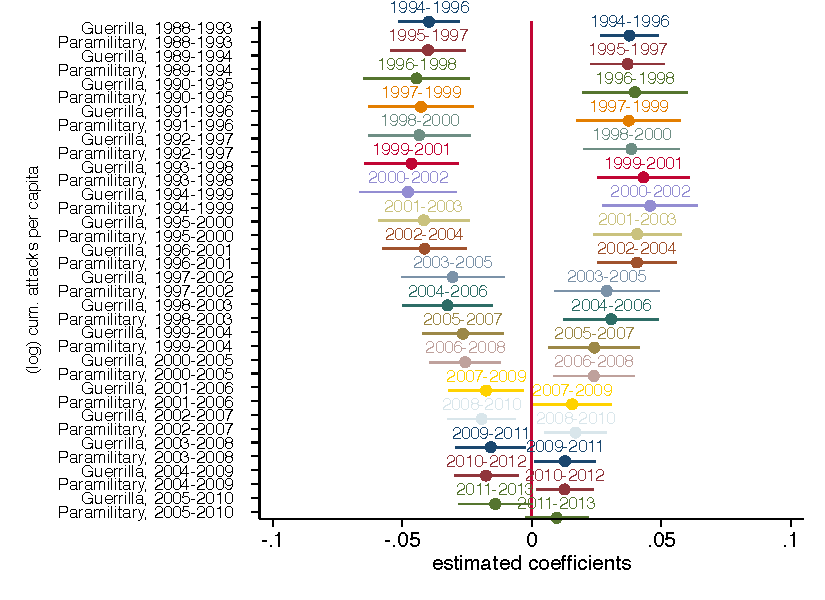
\includegraphics[width=1\textwidth]{Chapter3/Figures/figureE7.pdf}
\end{center}
\end{figure}

%--------------------------------
% FIGURE E2. EIGHT YEAR WINDOW
%--------------------------------

\begin{figure}[H]
\begin{center}
\caption{Estimated relationship between property tax revenues and attacks per armed group across Colombian municipalities, by time period using a moving window of 8 years}
\small{Dependent variable: (log) property tax revenue per capita (in the following 5-years)}
\label{appendix3:moving_window_8years}
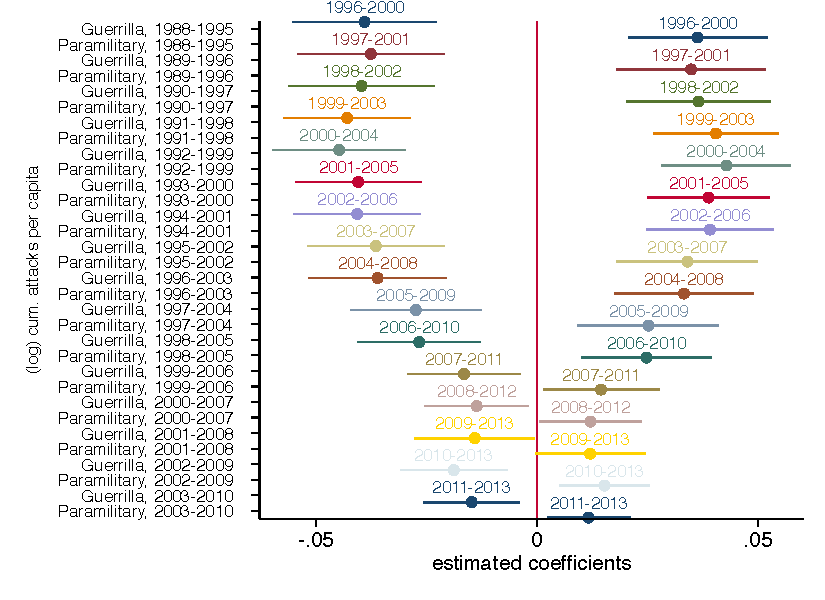
\includegraphics[width=1\textwidth]{Chapter3/Figures/figureE8.pdf}
\end{center}
\end{figure}

\newpage

%--------------------------------
\section{Multiple-testing correction \label{appendix3:multiple_test}}
%--------------------------------

The diversity of time periods, outcomes and mechanisms over the same dataset calls for the use of multiple-testing procedures to control for the familywise error rate (FWER), i.e. ``the probability of rejecting at least one true null hypothesis in a \emph{family} of tests'' (\citet{dafoeetal2017}). These procedures control for the inflation in false-positive error rates since there's a dependence across tests which increases the probability of getting a significant result by chance. Thus, we rely on three methods to deal with the multiple-testing problem: first, the Bonferroni correction -the most conservative approach- that adjusts the significance level $\alpha$ by setting the significance cut-off at $\alpha/n$, with $n$ the number of tests; second, the Hold correction, a less conservative approach to deal with the FWER, where after ordering the $j$ p-values from smallest to largest, selects the smallest one that would satisfy the condition $p_k > \alpha/(j+1-k)$, with $k$ the p-value's index, and from this level establishes a threshold at which smaller p-values are deemed as significant; lastly, the Benjamini-Hochberg procedure that controls for the False Discovery Rate (FDR), i.e. the expected proportion of false discoveries among all discoveries, where, after ordering the $j$th p-values, we find the largest one that satisfies the condition $p_k \leq (k/m)*\alpha$, and deems as significant all those lower than such threshold. 

Table \ref{appendix3:multiple_test_table} presents the correction results of the three procedures on the tests ran on Table \ref{chapter3_tab:main}, i.e. the relationships between cumulative attacks and tax revenues across four different time periods. The multiplication of time periods generates the aforementioned multiple-testing problem, thus pointing to the need for controlling for the FWER. After tacking into account the dependency across the 4 time periods, we note that even under the most conservative correction, i.e. Bonferroni, we still observe significant results for both treatment variables, and interestingly loose the significance in the last two periods where substantively we where not expecting results as is already noted in the main body of the paper (particularly in the last period). Note that under the Benjamini-Hochberg procedure, we still have significance for guerrilla attacks on the third period but not for paramilitaries, as expected. 

Furthermore, Table \ref{appendix3:multiple_test_table2} presents the correction comparisons and contrast to the target p-value $\alpha$ of 5\% for those tests that share the same treatment and outcome time period, 1997-2002 and 2003-2006, respectively. Given the diversity of mechanisms and outcomes over the same time period a concern is raised over the FWER. Correction results take into account all the outcomes of Tables \ref{chapter3_tab:main}, \ref{chapter3:table3}, \ref{chapter3:table4}, \ref{appendix3:consequences_violence} and \ref{appendix3:consequences_economic}, i.e. 11 tests. Results show that for the main outcome, property tax revenue per capita from Table \ref{chapter3_tab:main}, mechanisms of Table \ref{chapter3:table3}, and outcomes of Table \ref{appendix3:consequences_violence} (social outcomes), remain significant after the Bonferroni correction, and the number of significant tests increases when tacking into account either the Holm correction and the Benjamini-Hachberg procedure. No significant results are found for nighttime light data estimates (Table \ref{appendix3:consequences_economic}) either using 11 tests or 4 adjusting for 4 time periods, or for electoral outcomes after correction, except for the significance of the win dummy variable for Mayor election under the Benjamini-Hachberg procedure in column (9). 

\begin{table}[H]
\centering
\caption{Multiple-testing: corrections comparison and contrast to target p-value $\alpha$ of 5\% \\ \small{-Tests from Table \ref{chapter3_tab:main}-}}
\label{appendix3:multiple_test_table}
\scalebox{0.7}{
\begin{tabular}{lccccc}
 & \multicolumn{4}{c}{\textbf{Outcome}} &  \\ \cline{2-5}
DV: & \multicolumn{4}{c}{\textit{(log) property tax revenue per capita}} &  \\
DV time period: & 1997-2002 & 2003-2006 & 2007-2010 & 2011-20013 & \textbf{\begin{tabular}[c]{@{}c@{}}Statistically\\ \\ significant\end{tabular}} \\ \cline{2-5}
\textit{Benjamini-Hochberg procedure:} &  &  &  &  &  \\ \cline{1-1}
\begin{tabular}[c]{@{}l@{}}(log) cum. guerrilla attacks \\ per capita, over respective period\\ (1988-1996; 1997-2002;\\ 2003-2006; 2007-2010)\end{tabular} & \checkmark & \checkmark & \checkmark &  & 3/4 \\
\begin{tabular}[c]{@{}l@{}}(log) cum. paramilitary attacks \\ per capita, over respective period\\ (1988-1996; 1997-2002;\\ 2003-2006; 2007-2010)\end{tabular} & \checkmark & \checkmark &  &  & 2/4 \\
 &  &  &  &  &  \\
\textit{Holm correction:} &  &  &  &  &  \\ \cline{1-1}
\begin{tabular}[c]{@{}l@{}}(log) cum. guerrilla attacks \\ per capita, over respective period\\ (1988-1996; 1997-2002;\\ 2003-2006; 2007-2010)\end{tabular} & \checkmark & \checkmark &  &  & 2/4 \\
\begin{tabular}[c]{@{}l@{}}(log) cum. paramilitary attacks \\ per capita, over respective period\\ (1988-1996; 1997-2002;\\ 2003-2006; 2007-2010)\end{tabular} & \checkmark & \checkmark &  &  & 2/4 \\
 &  &  &  &  &  \\
\textit{Bonferroni correction:} &  &  &  &  &  \\ \cline{1-1}
\begin{tabular}[c]{@{}l@{}}(log) cum. guerrilla attacks \\ per capita, over respective period\\ (1988-1996; 1997-2002;\\ 2003-2006; 2007-2010)\end{tabular} & \checkmark & \checkmark &  &  & 2/4 \\
\begin{tabular}[c]{@{}l@{}}(log) cum. paramilitary attacks \\ per capita, over respective period\\ (1988-1996; 1997-2002;\\ 2003-2006; 2007-2010)\end{tabular} & \checkmark & \checkmark &  &  & 2/4 \\ \hline
\end{tabular}
}
\end{table}

\small{Note: This table presents multiple-testing corrections comparisons, and contrast to the target p-value of 5\%. It takes into account the 4 tests presented in Table \ref{chapter3_tab:main}. A \checkmark states a significant corrected estimate. Specifications used are the same as those found across Tables \ref{chapter3_tab:main}.} 

\begin{landscape}
\begin{table}[H]
\centering
\caption{Multiple-testing: corrections comparison and contrast to target p-value $\alpha$ of 5\% \\ \small{-Tests with treatment over period 1997-2002-}}
\label{appendix3:multiple_test_table2}
\scalebox{0.45}{
\begin{tabular}{lcccccccccccc}
 & \multicolumn{11}{c}{\textbf{Outcome}} &  \\ \cline{2-12}
\multicolumn{1}{c}{DV: time} & \multicolumn{11}{c}{\textit{2003-2006}} &  \\
\multicolumn{1}{c}{DV:} & \begin{tabular}[c]{@{}c@{}}Property\\  tax\\ revenue\end{tabular} & \begin{tabular}[c]{@{}c@{}}Per capita\\  land\\ value\end{tabular} & \begin{tabular}[c]{@{}c@{}}Cadastral\\  update\\ lag\end{tabular} & \begin{tabular}[c]{@{}c@{}}No. of\\  cadastral\\ updates\\  per capita\end{tabular} & \begin{tabular}[c]{@{}c@{}}Land \\ informality\\ rate\end{tabular} & \begin{tabular}[c]{@{}c@{}}Secondary \\ enrollmente\end{tabular} & \begin{tabular}[c]{@{}c@{}}Quality of\\  education\\ (math test)\end{tabular} & \begin{tabular}[c]{@{}c@{}}Nighttime\\  light\\ per capita\end{tabular} & \begin{tabular}[c]{@{}c@{}}Win\\ dummy,\\ Mayor \\ election\end{tabular} & \begin{tabular}[c]{@{}c@{}}Vote\\  share, \\ Mayor election\end{tabular} & \begin{tabular}[c]{@{}c@{}}Vote\\  share, \\ City \\ Council election\end{tabular} & \textbf{\begin{tabular}[c]{@{}c@{}}Statistically\\  significant\end{tabular}} \\ 
&(1) &(2)  &(3) &(4) &(5) &(6) &(7) &(8) &(9) &(10) &(11) \\
\cline{2-12}
\textit{Benjamini-Hochberg procedure:} &  &  &  &  &  &  &  &  &  &  &  &  \\ \cline{1-1}
\begin{tabular}[c]{@{}l@{}}(log) cum. guerrilla attacks \\ per capita, 1997-2002\end{tabular} & \checkmark & \checkmark & \checkmark & \checkmark & \checkmark & \checkmark & \checkmark &  & \checkmark &  &  & 8/11 \\
\begin{tabular}[c]{@{}l@{}}(log) cum. paramilitary attacks \\ per capita, 1997-2002:\end{tabular} & \checkmark & \checkmark & \checkmark & \checkmark & \checkmark & \checkmark & \checkmark &  & \checkmark &  &  & 8/11 \\
 &  &  &  &  &  &  &  &  &  &  &  &  \\
\textit{Holm correction:} &  &  &  &  &  &  &  &  &  &  &  &  \\ \cline{1-1}
\begin{tabular}[c]{@{}l@{}}(log) cum. guerrilla attacks \\ per capita, 1997-2002\end{tabular} & \checkmark & \checkmark & \checkmark & \checkmark & \checkmark & \checkmark & \checkmark &  &  &  &  & 7/11 \\
\begin{tabular}[c]{@{}l@{}}(log) cum. paramilitary attacks \\ per capita, 1997-2002:\end{tabular} & \checkmark & \checkmark & \checkmark & \checkmark & \checkmark & \checkmark & \checkmark &  &  &  &  & 7/11 \\
 &  &  &  &  &  &  &  &  &  &  &  &  \\
\textit{Bonferroni correction:} &  &  &  &  &  &  &  &  &  &  &  &  \\ \cline{1-1}
\begin{tabular}[c]{@{}l@{}}(log) cum. guerrilla attacks \\ per capita, 1997-2002\end{tabular} & \checkmark & \checkmark & \checkmark & \checkmark & \checkmark & \checkmark & \checkmark &  &  &  &  & 7/11 \\
\begin{tabular}[c]{@{}l@{}}(log) cum. paramilitary attacks\\ per capita, 1997-2002\end{tabular} & \checkmark & \checkmark & \checkmark & \checkmark & \checkmark &  & \checkmark &  &  &  &  & 6/11 \\ \hline
\end{tabular}

}
\end{table}
Note: This table presents multiple-testing corrections comparisons, and contrast to the target p-value of 5\%. It takes into account the 11 tests covered on the same time period, with the treatment variables running from 1997 to 2002, and outcome variables from 2003 to 2006. A \checkmark states a significant corrected estimate. Specifications used are the same as those found across Tables 2-4, \ref{appendix3:consequences_violence} and G2. 
\end{landscape}

\clearpage

\section{``Why This Matters'' \label{appendix3:why_matters}}

\subsection{Effect on social outcomes \label{appendix3:effect_social}}

Understanding the determinants of why some places are much better at collecting taxes than others is important for policy purposes. Municipalities in Colombia are responsible for providing a wide range of social goods that are likely to be affected by captured tax institutions. For instance, if tax revenues increase and they are invested in local social goods, then their quality should improve. In order to assess the effect of armed group presence on social outcomes, we evaluate educational outcomes for two reasons. First, educational outcomes  are very well measured at the municipal level in Colombia, and provide us a good way to gage the effect on social outcomes. On the other hand, their service might be more influenced by local dynamics relative to other public services that are dependent on national transfers and royalties. 

In this line, Table \ref{appendix3:consequences_violence} shows further that both guerrilla and paramilitary activity appear to have an asymmetric effect --consistent with the findings on tax revenues and tax institutions-- on educational attainment as well as education quality, as measured by the score in a standardized tests taken by all students finishing high school in the country (called SABER 11). Using the most demanding specification of column 2 of Table \ref{appendix3:consequences_violence}, an increase in cumulative per capita guerrilla attacks (paramilitary attacks) over the period 1997-2002 from the median to the 90$^{th}$ percentile of the distribution, is associated with an average drop (increase) of 19.6\% (17.2\%) of a standard deviation in the secondary enrollment rate over the period 2003-2006. The effect of a similar change on the quality of education as measured by the score in the math chapter of SABER 11 is a drop (increase) of 28\% (22\%) of a standard deviation for the case of cumulative guerrilla (paramilitary) attacks.

\subsection{Effect on economic activity \label{appendix3:effect_economic}}

To the best of our knowledge, no article has analyzed potential differential effects of guerrilla and paramilitary violence on economic activity.\footnote{\citet{riascosvargas2011} provide a thorough review the literature on the effect of armed conflict on economic performance in Colombia.}

In this appendix we investigate the effect of our cumulative conflict measure on local-level development, as measured by nighttime light  intensity, normalized by population. We find that cumulative violence perpetrated by guerrillas is consistently negatively associated with economic activity, while violence by paramilitaries is positively correlated, at least during the periods 2003-2006 and 2007-2010. 

Following the structure of Table \ref{chapter3_tab:main}, Table \ref{appendix3:consequences_economic} reports the estimates of the statistical association between guerrilla and paramilitary cumulative past violence and economic performance.

Odd columns show that the association between armed activity and economic performance is asymmetric across armed group: guerrilla cumulative attacks per capita have a negative relationship with economic activity (which is significant only in the second period) while paramilitary attacks show a positive
relationship (significant in all four periods). These results are, however, not robust to controlling for pre-period luminosity per capita (except in the third period for paramilitary attacks).

If we take into account the effect for the treatment period from 2003 - 2006 on 2007 - 2010 outcome, we notice a substantial asymmetric association. Because of the log-log specification, estimated coefficients should be interpreted as the elasticity of per capita property tax revenue with respect to cumulative past violence. 

Using the most demanding specification of column 6, an increase in cumulative per capita paramilitary attacks over the period 2003-2006 from the median to the 90$^{th}$ percentile of the distribution is associated with an average 3.5\% increase in nighttime lights over the period 2007-2010. 


\bigskip

% Table G1. Consequences: Cumulative violence (1997-2002) and social outcomes (2003-2006)

%\begin{landscape}
\begin{table}[htbp]
\def\sym#1{\ifmmode^{#1}\else\(^{#1}\)\fi}\caption{Consequences: Cumulative violence (1997-2002) and social outcomes (2003-2006)}
\label{appendix3:consequences_violence}
\begin{center}
\scalebox{0.65}{
\begin{tabular}{lccccc}
\hline \hline 
  & (1) & (2) & (3) & (4)   \\
 \hline 
 \\ 

 &\multicolumn{2}{c}{\emph{Secondary enrollment}}&\multicolumn{2}{c}{\emph{Quality of edu. (math test)}}\\\cmidrule(lr){2-3}\cmidrule(lr){4-5}
\addlinespace
\begin{tabular}[c]{@{}l@{}}Log guerrilla attacks\\ per capita \underline{1997-2002}\end{tabular}&     -0.0171\sym{***}&     -0.0088\sym{***}&     -0.0115\sym{***}&     -0.0092\sym{***}\\
            &    (0.0024)         &    (0.0021)         &    (0.0018)         &    (0.0018)         \\
\addlinespace
\begin{tabular}[c]{@{}l@{}}Log paramilitary attacks\\ per capita \underline{1997-2002}\end{tabular}&      0.0157\sym{***}&      0.0077\sym{***}&      0.0093\sym{***}&      0.0070\sym{**} \\
            &    (0.0024)         &    (0.0021)         &    (0.0019)         &    (0.0020)         \\
\addlinespace
Observations&        1071         &        1071         &         949         &         949         \\
R-squared   &       0.342         &       0.417         &       0.411         &       0.420         \\
Controls$^a$&  \checkmark         &  \checkmark         &  \checkmark         &  \checkmark         \\
Depto. FE   &  \checkmark         &  \checkmark         &  \checkmark         &  \checkmark         \\
Pre-period DV$^b$&                     &  \checkmark         &                     &  \checkmark         \\




\hline \hline 
\multicolumn{5}{p{1\textwidth}}{\footnotesize{Notes: Standard errors in parentheses are clustered at the department level; Significance-level: $^{***}$ 0.1\%; $^{**}$ 1\%; $^*$ 5\%; and $^{+}$ 10\%, refers to two-sided t-tests. 
$^a$Controls as in Table \ref{chapter3_tab:main}.
$^b$Due to the lack of quality of education data for the 1993-1996 period, we included the pre-period property tax revenue per capita from 1993 to 1996 in columns (2) and (4), to pick up part of the enduring cross-sectional within-department differences.}} \\
\end{tabular}
}
\end{center}
\end{table}
%\end{landscape}
%-----------------------------------------------------------%
\newpage

% Table G2. Consequences: Cumulative violence and economic activity

%\begin{landscape}
\begin{table}[htbp]
\def\sym#1{\ifmmode^{#1}\else\(^{#1}\)\fi}
\caption{Consequences: Cumulative violence and economic activity}
\label{appendix3:consequences_economic}
\begin{center}
\scalebox{0.65}{
\begin{tabular}{lcccccccc}
\hline \hline 
\multicolumn{9}{l}{Dependent variable: {\it Log of nighttime light per capita} over period:}\\

 &\multicolumn{2}{c}{1997-2002}              &\multicolumn{2}{c}{2003-2006}              &\multicolumn{2}{c}{2007-2010}              &\multicolumn{2}{c}{2011-2013}              \\\cmidrule(lr){2-3}\cmidrule(lr){4-5}\cmidrule(lr){6-7}\cmidrule(lr){8-9}
            &\multicolumn{1}{c}{(1)}         &\multicolumn{1}{c}{(2)}         &\multicolumn{1}{c}{(3)}         &\multicolumn{1}{c}{(4)}         &\multicolumn{1}{c}{(5)}         &\multicolumn{1}{c}{(6)}         &\multicolumn{1}{c}{(7)}         &\multicolumn{1}{c}{(8)}         \\
\addlinespace
\begin{tabular}[c]{@{}l@{}}Log guerrilla attacks\\ per capita \underline{1988-1996}\end{tabular}&     -0.0126         &      0.0008         &                     &                     &                     &                     &                     &                     \\
            &    (0.0125)         &    (0.0037)         &                     &                     &                     &                     &                     &                     \\
\addlinespace
\begin{tabular}[c]{@{}l@{}}Log paramilitary attacks\\ per capita \underline{1988-1996}\end{tabular}&      0.0314\sym{*}  &      0.0012         &                     &                     &                     &                     &                     &                     \\
            &    (0.0117)         &    (0.0032)         &                     &                     &                     &                     &                     &                     \\
\addlinespace
\begin{tabular}[c]{@{}l@{}}Log guerrilla attacks\\ per capita \underline{1997-2002}\end{tabular}&                     &                     &     -0.0269\sym{*}  &     -0.0003         &                     &                     &                     &                     \\
            &                     &                     &    (0.0103)         &    (0.0033)         &                     &                     &                     &                     \\
\addlinespace
\begin{tabular}[c]{@{}l@{}}Log paramilitary attacks\\ per capita \underline{1997-2002}\end{tabular}&                     &                     &      0.0458\sym{***}&      0.0016         &                     &                     &                     &                     \\
            &                     &                     &    (0.0098)         &    (0.0034)         &                     &                     &                     &                     \\
\addlinespace
\begin{tabular}[c]{@{}l@{}}Log guerrilla attacks\\ per capita \underline{2003-2006}\end{tabular}&                     &                     &                     &                     &     -0.0084         &     -0.0052         &                     &                     \\
            &                     &                     &                     &                     &    (0.0099)         &    (0.0031)         &                     &                     \\
\addlinespace
\begin{tabular}[c]{@{}l@{}}Log paramilitary attacks\\ per capita \underline{2003-2006}\end{tabular}&                     &                     &                     &                     &      0.0364\sym{***}&      0.0070\sym{*}  &                     &                     \\
            &                     &                     &                     &                     &    (0.0086)         &    (0.0030)         &                     &                     \\
\addlinespace
\begin{tabular}[c]{@{}l@{}}Log guerrilla attacks\\ per capita \underline{2007-2010}\end{tabular}&                     &                     &                     &                     &                     &                     &     -0.0193         &      0.0144         \\
            &                     &                     &                     &                     &                     &                     &    (0.0220)         &    (0.0090)         \\
\addlinespace
\begin{tabular}[c]{@{}l@{}}Log paramilitary attacks\\ per capita \underline{2007-2010}\end{tabular}&                     &                     &                     &                     &                     &                     &      0.0469\sym{*}  &     -0.0069         \\
            &                     &                     &                     &                     &                     &                     &    (0.0195)         &    (0.0079)         \\
\addlinespace
Observations&        1028         &        1028         &        1045         &        1045         &        1048         &        1048         &        1048         &        1048         \\
R-squared   &       0.547         &       0.920         &       0.600         &       0.953         &       0.660         &       0.975         &       0.665         &       0.963         \\
Controls$^a$&  \checkmark         &  \checkmark         &  \checkmark         &  \checkmark         &  \checkmark         &  \checkmark         &  \checkmark         &  \checkmark         \\
Depto. FE   &  \checkmark         &  \checkmark         &  \checkmark         &  \checkmark         &  \checkmark         &  \checkmark         &  \checkmark         &  \checkmark         \\
Pre-period DV$^b$&                     &  \checkmark         &                     &  \checkmark         &                     &  \checkmark         &                     &  \checkmark         \\


\hline \hline
\multicolumn{9}{p{1.4\textwidth}}{\footnotesize{Notes: Standard errors in parentheses are clustered at the department level; Significance-level: $^{***}$ 0.1\%; $^{**}$ 1\%; $^*$ 5\%; and $^{+}$ 10\%, refers to two-sided t-tests. 
$^a$ Controls as in Table \ref{chapter3_tab:main}.
$^b$ Estimations include pre-period logged luminosity per capita from 1992 in column (2), from 1992 to 1996 in (4), from 2000 to 2002 in (6), and from 2003 to 2006 in (8), to pick up part of the enduring cross-sectional within-department differences.}} \\
\end{tabular}
}
\end{center}
\end{table}
%\end{landscape}

\clearpage


\section{Civil war dynamics and capture in Colombia: the four periods in more detail} \label{fourperiods}

The dynamics of the civil war in terms of territorial control and violence have changed significantly over time.\footnote{Differences also exist within the groups across regions, we summarize the broad trends.}

We separate the war's recent evolution, and the armed groups' capture strategies, into four periods. We organize the statistical analysis around these four periods because pooling them would effectively assume that armed actors had the same ability to influence tax policies in every year, which strikes us as substantively unrealistic. Importantly, levels of violence and control by different groups varied across these periods, a fact that we exploit in our empirical strategy.

\textbf{1988-1996: FARC ascendancy}\\
The FARC increased its presence in the mid-1980s and 1990s. According to one estimate \citep[28]{echandia06a}, in 1985, the FARC had a presence in 173 of the country's roughly 1,120 municipalities, and by 1995 spread to 622. During this period, the FARC tried to influence policy directly by forming a political party, the Patriotic Union (UP), that began to contest local elections in 1988.  UP candidates won sixteen mayoral positions and 256 municipal council positions. Only two years later, though, the UP distanced itself from the FARC to protect itself from the violence targeted at them by paramilitary groups. By the end of the period, the FARC and the ELN both enforced election boycotts in areas under their control, and threatened elected mayors and local council members \citep{el-tiempo97a}. 

While some regional politicians supported paramilitaries' formation during this period \citep[37]{ronderos14a}, e.g. Pablo Emilio Guar\'{i}n from the Liberal party, there is little evidence that paramilitary groups tried to capture political institutions directly at the local level. This is not to say that there were no political impacts of paramilitary presence during this period. In areas experiencing paramilitary violence, like the Magdalena Medio and Urab\'{a}, high levels of displacement and political assassination were endemic. These processes surely affected the viability of some candidates and forms of politics during this period.  

\textbf{1997-2002: Paramilitary expansion}\\
In 1997, regional paramilitary groups united under the umbrella group United Self-Defense Forces of Colombia (AUC) and the war spread. By 2001, the AUC was powerful enough to convene a meeting with nearly 100 politicians to formulate a concerted effort to win elections at all levels, and to support \'Alvaro Uribe's candidacy for president in 2002 (known as the Santa Fe de Ralito pact). According to the attorney general's office, the Sante Fe de Ralito pact was an effort by the paramilitaries to use their ``consolidated'' military and economic power at the local levels ``to influence the Congress as a political actor and prepare for an eventual negotiation process'' \citep{verdad-abierta15a}. 

The details of how this effort played out are informative about how military power was transformed into political influence.\footnote{Vicente Casta\~{n}o, one of the brothers behind the formation of the AUC, apparently ordered AUC blocks to enter politics, with the idea that the groups would be recognized as political organizations rather than drug traffickers, and be eligible for more lenient criminal charges as a result \citep{ronderos14a}.} 
One commander in Urab\'{a} excelled at political organizing: Fredy Rend\'{o}n Herrera, alias `El Alem\'{a}n' (The German), and head of the Elmer C\'{a}rdenas block (ECB). The block entered the northern region of Urab\'{a} and accompanied the army's ``Operation Genesis,'' which involved the mass displacement of many communities and the eventual takeover by the paramilitaries. In 2000, El Alem\'{a}n began to train wounded combatants as ``Social Development Promoters'' to organize communities under their control, and specifically to form JACs and carry out projects together, such as road and bridge building \citep{verdad-abierta15b}. The JACs were then used as the basis for electoral influence: ahead of the 2001 elections, they convened assemblies within communities to choose candidates for the municipal councils. For mayor, El Alem\'{a}n reported in his confession to authorities that the strategy was to select two candidates: one with similar ideological preferences as the AUC, and one that had little political clout, so could easily be controlled. By 2010, 25 politicians from the region were convicted of collaboration with the paramilitaries. The block also engaged in electoral coercion, according to \citet{avila-martinez10a}.\footnote{The paramilitaries also formed a political alliance with municipal governments in the region called ``For a Big, United Urab\'{a} at Peace.'' VerdadAbierta.com, an investigative journalism organization, reported that the Elmer C\'{a}rdenas block used its political connections to ``take advantage of the productive projects [related to coca eradication] as well as the public finances of the municipalities under its control.'' The block even evaluated projects presented to the municipal council, or proposed its own projects, according to one ex-combatant's testimony. In 2002, the block also formed a non-profit organization called ASOCOMUN, which competed and won municipal contracts and grants from the central government \citep{verdad-abierta15b}. Finally, by 2002, the AUC decided to support particular candidates for Congress, in order to try to influence a favorable demobilization agreement with the government. All candidates backed by El Alem\'{a}n in Urab\'{a} were elected \citep{verdad-abierta11a}.} 

Compared to the paramilitaries, the FARC's influence remained indirect. The FARC largely continued to eschew official electoral politics during this period, preferring to target municipal candidates that the group did not approve of, or acting mayors. This targeting presumably created strong incentives for local politicians in areas of dominant FARC presence to shift their policies towards the group's preferences. A key exception is the territory it governed directly during peace talks with the Pastrana administration (1998-2002). Known as the \emph{Zona de Despeje}, the territory included 6 municipalities and was roughly the size of Maryland. During this period, the FARC enacted \emph{Ley 002} to govern taxation, which stipulated who would be taxed (the wealthy), and the consequences for not paying (kidnapping) \citep{farcley2005}. The first article of the law established the tax collection for those individuals or companies with assets worth more than a million dollars, without specifying the rate, while the second article stated that failing to pay the stated tax would imply an increase of the tax amount (again without stating the tax value and rate). Finally, according to the third article of the law, those that didn't comply would be detained until a suitable payment would be made (\citet{farcley2005}). . In 2002, the Pastrana administration ended peace talks and reentered the Maryland-sized zone comprising six municipalities it had ceded to the FARC during the talks, known as the. FARC tax policy in the \emph{despeje} provides evidence of its preferences for informality and favoritism of the poor and landless.
This was an extension of the FARC's early practice of taxing the local population in areas where it established its earliest presence \citep{molano87a}. 

\textbf{2003-2006: Paramilitary demobilization} \\
In 2003, the Uribe administration negotiated a ceasefire with paramilitary groups and eventually adopted the {\it Justice and Peace law}. The law allowed paramilitary commanders to demobilize their troops in exchange for lenient sentences, with a maximum of eight years total possible prison time.\footnote{Uribe also extradited 14 commanders to the US in 2008 for failing to comply with the condition of confessing all of their crimes; they are now serving longer prison sentences for drug trafficking convictions.} 
Paramilitary demobilizations began in 2003 and reached a peak in 2005, which officially transformed the war into a contest between the state and remaining insurgent groups (the FARC and ELN). In total, by 2006, 37 paramilitary blocks had demobilized \citep{altocomisionado06}. 

In spite of the demobilization program, some groups remained active and continued to exert an influence on local politics. For example, the ECB continued to influence local politics through 2006, including ``check-ins'' with the mayors' secretaries \citep{verdad-abierta11a}. According to one former paramilitary commander's confession, the point was not to control the mayoral offices, but to ``help them deliver development to the people'' \citep{verdad-abierta11a}.  

The conflict with the FARC continued apace during this period, but there was no clear change in terms of capture strategy. In Urab\'{a}, for example, El Alem\'{a}n's block continued to deepen its influence in local politics, and also turned their attention to the national level, through pacts with regional political elites \citep{gutierrez-sanin10c, lopez-hernandez10a}. They formed groups of candidates who would rotate in office, one year at a time \citep{verdad-abierta11a}. Interestingly, none of the three candidates for Congressional representative backed by the Elmer C\'{a}rdenas block won election for the 2006-2010 period (candidates for Senate, elected at large, however, did receive unusually high vote shares in the region). At the local level, ASOCOMUN continued to win grants and contracts, amounting to what VerdadAbierta.com calculated was \$1.607 million pesos (roughly \$500k).

\textbf{2007-2010: State resurgence}\\
Besides the remaining left-wing guerrilla groups, many former paramilitary groups morphed into new organizations, including the ``Black Eagles,'' and drug-trafficking groups such as the ``Urabe\~{n}os'' and the ``Rastrojos.'' All of these groups sometimes engaged in actions against the FARC, the ELN, and the civilian population. \footnote{See \citet{daly16a} for an account of the variation in post-demobilization trajectories and the emergence of criminal bands (BACRIMs).} Some have also attacked leaders of groups seeking land restitution, presumably to block efforts to invalidate titles that were acquired through coercion or violence \citep{amnesty-international14a}. 

Under Uribe, the Colombian military and police redeployed to major population centers and roads, improving measures of security. In addition, government forces killed several members of the FARC's secretariat, including Alfonso Cano, who had taken over the leadership of the group following Manuel Marulanda's death in 2008. The weakened FARC agreed to peace talks following the 2010 election of Uribe's Minister of Defense, Juan Manuel Santos. 






%% Note: If your thesis has more than one appendix, NYU requires a "list of
%% appendices" page before the body of the thesis. I don't provide the tools
%% to create that here, so you're on your own for that one... Sorry.
%\chapter{Appendix of ``Love the Candidate but Hate his Party: The Asymmetric Effects of Reelection Incentives on Partisan and Personal Incumbency Returns in Mexico'' \label{chap:append2}}

\break

%\section{Tables and Figures}

\begin{table}[H]
\centering 
\caption{Descriptive statistics}
   
\label{tab:descriptive}
\scalebox{0.55}{ 
{
\def\sym#1{\ifmmode^{#1}\else\(^{#1}\)\fi}
\begin{tabular}{l*{1}{ccccc}}
\hline\hline
            &        \textbf{Mean}&  \textbf{SD}&  \textbf{Min}&  \textbf{Max}& \textbf{N}\\
\hline    
\emph{Pane A - Incumbency Advantage:} 	&		&		&		&		\\
Probability of winning, election at t+1&        0.40&        0.49&           0&           1&       2,247\\
Vote share, election at t+1&       -0.05&        0.18&          -1&         .59&       2,246\\

\\
\emph{Panel B - Treatments and Forcing Variable:} 	&		&		&		&		\\
Term Limit Removed=1; 0 otherwise&        0.29&        0.45&           0&           1&       2,247\\
Win election at t=1; 0 otherwise&        0.46&        0.50&           0&           1&       2,247\\

Winning margin: first - second runner&        0.07&        0.05&        0.00&        0.33&       2,247\\


\\
\emph{Panel C - Pretreatment controls:} 	&		&		&		&		\\
Winning margin: first - second runner (governor)&        0.15&        0.13&           0&           1&      24,470\\
Party alignment with federal executive=1; 0 otherwise&        0.54&        0.50&           0&           1&      24,470\\

Population (INEGI and CONAPO projections)&      49,233&     129,415&         409&   1,714,709&       2,247\\


\\
\emph{Panel D - Mechanisms-Fiscal Transfers:} 	&		&		&		&		\\
General Participations Fund (Mill. pesos)&          39&          94&         .81&       1,221&       1,638\\
Participating Fund (Mill. pesos)&          52&         127&         .21&       1,498&       1,656\\
Municipal Development Fund (Mill. pesos)&         9.7&          24&          .2&         345&       1,642\\
Federal and state contributions (Mill. pesos)&          60&         131&        .048&       2,133&       1,768\\
Contribution Fund for Municipal Social Infrastructure (Mill. pesos)&          18&          30&        .048&         618&       1,759\\
Contribution Fund to Strengthen Municipalities (Mill. pesos)&          23&          61&         .15&         865&       1,755\\

\\
\emph{Panel E - Mechanisms-Municipal Revenues:} 	&		&		&		&		\\
Total Municipal Revenues (Mill. pesos)&         166&         420&           2&       5,715&       1,779\\
Tax Revenues (Mill. pesos)&          19&          82&      .00017&       1,256&       1,735\\
Property Tax Rrevenues (Mill. pesos)&          12&          48&      .00013&         476&       1,360\\
Estate Tax Revenues (Mill. pesos)&          17&          66&      .00013&         672&       1,506\\
Prod., Cons. and Trans. Tax Revenues (Mill. pesos)&         1.2&          19&     .000096&         488&         671\\
Vehicle Ownership Tax Revenues (Mill. pesos)&          .5&         1.9&     .000081&          29&       1,324\\
New Cars Tax Revenues (Mill. pesos)&         .87&         2.9&       .0032&          49&       1,530\\
Public Security Revenues (Mill. pesos)&         6.1&          15&     .000078&         121&         211\\

\\
\emph{Panel F - Mechanisms-Other Resources:} 	&		&		&		&		\\
Number of City Council Sessions&          23&          19&           0&         288&       1,784\\
Number of Approved Initiatives of Law&          17&          32&           0&         295&         884\\
Percentage of Municipal Budget Spend&          11&          15&           0&         100&         789\\
Bureaucrats per 100,000 inhabitants&       1,945&       2,601&           0&      24,528&       1,247\\

\\
\emph{Panel G - Mechanisms-Incumbents' quality:} 	&		&		&		&		\\
Incumbent undergraduate or graduate title (indicator)&        0.06&        0.24&           0&           1&      19,430\\

\\ 

\hline\hline
\end{tabular}    
}
}
\end{table} 
   


 \begin{figure}[h]   
\centering
 \caption{No discontinuous jump of covariates}
 \label{fig:jump_covariates}
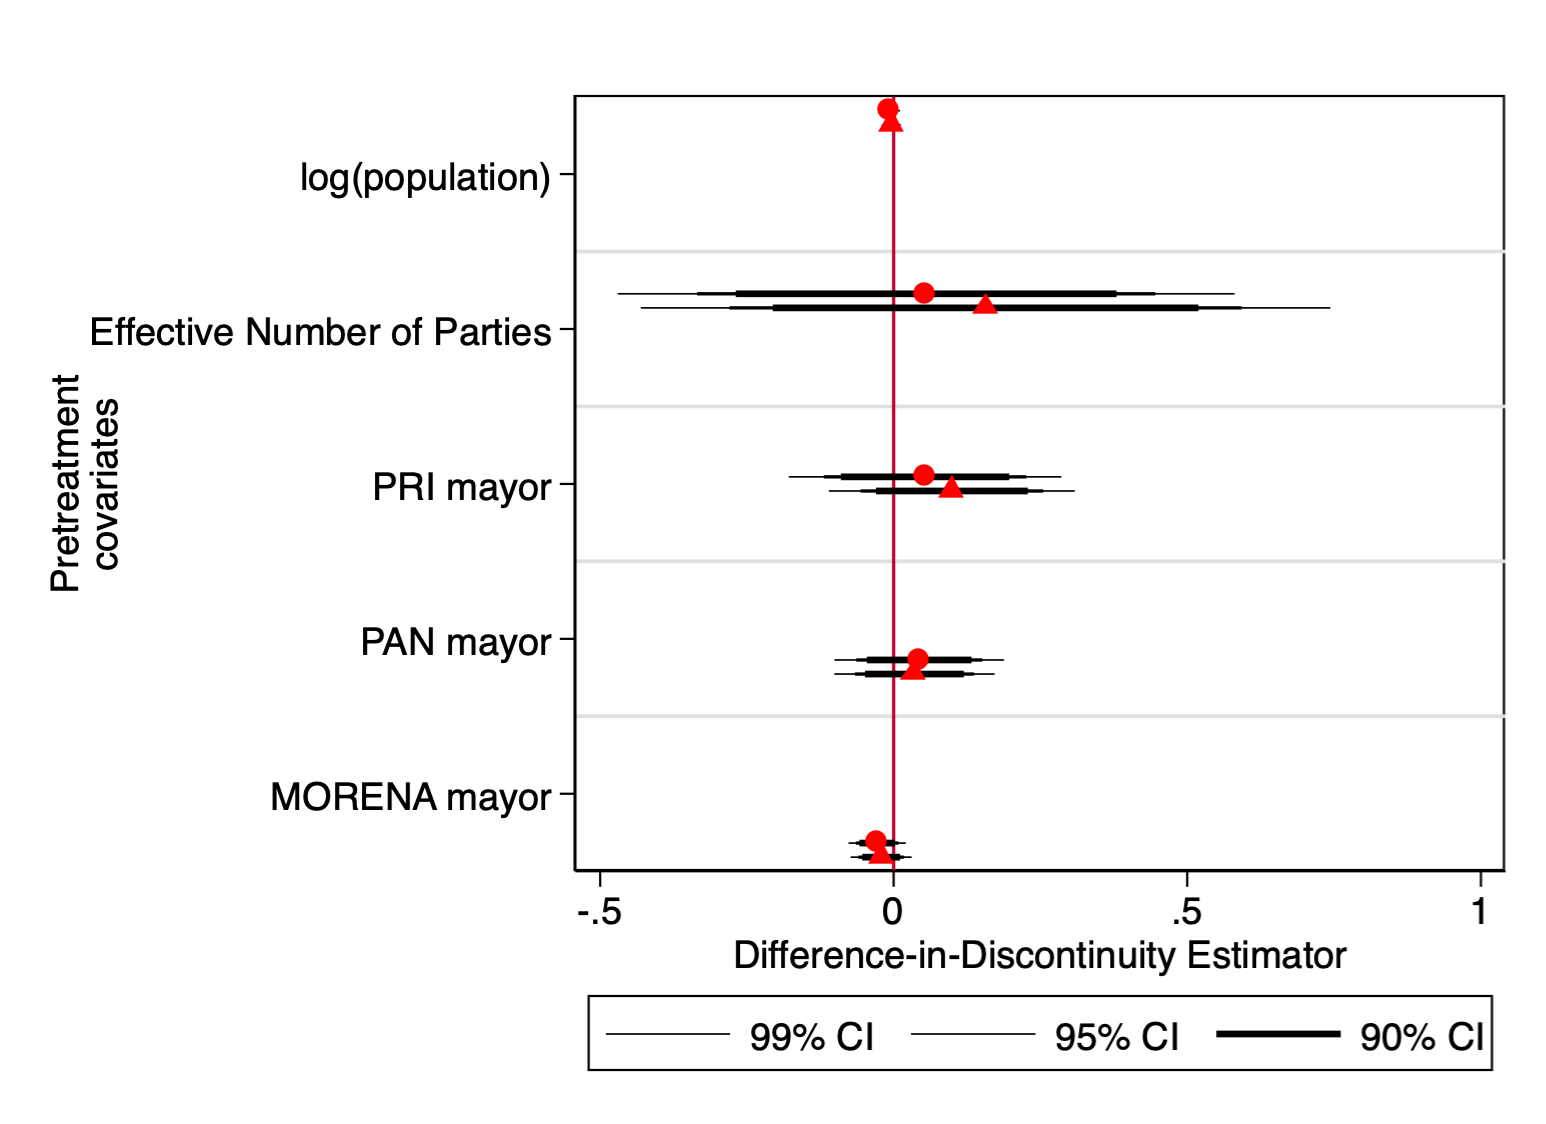
\includegraphics[width=0.9\textwidth]{Chapter2/Figures_incumbency/nojump.png}
       \captionsetup{justification=centering}
    
 \textbf{Note:} Figure \ref{fig:jump_covariates} shows the average treatment effect of the Term Limit Reform on various pretreatment covariates using a difference in discontinuity of close elections design. Optimal bandwidths following \citet{calonicoetal_2014} are used. 
   
\end{figure} 

  
    
    
\begin{figure}[h]   
\centering
 \caption{McCrary Test}
 \label{fig:mccrary}
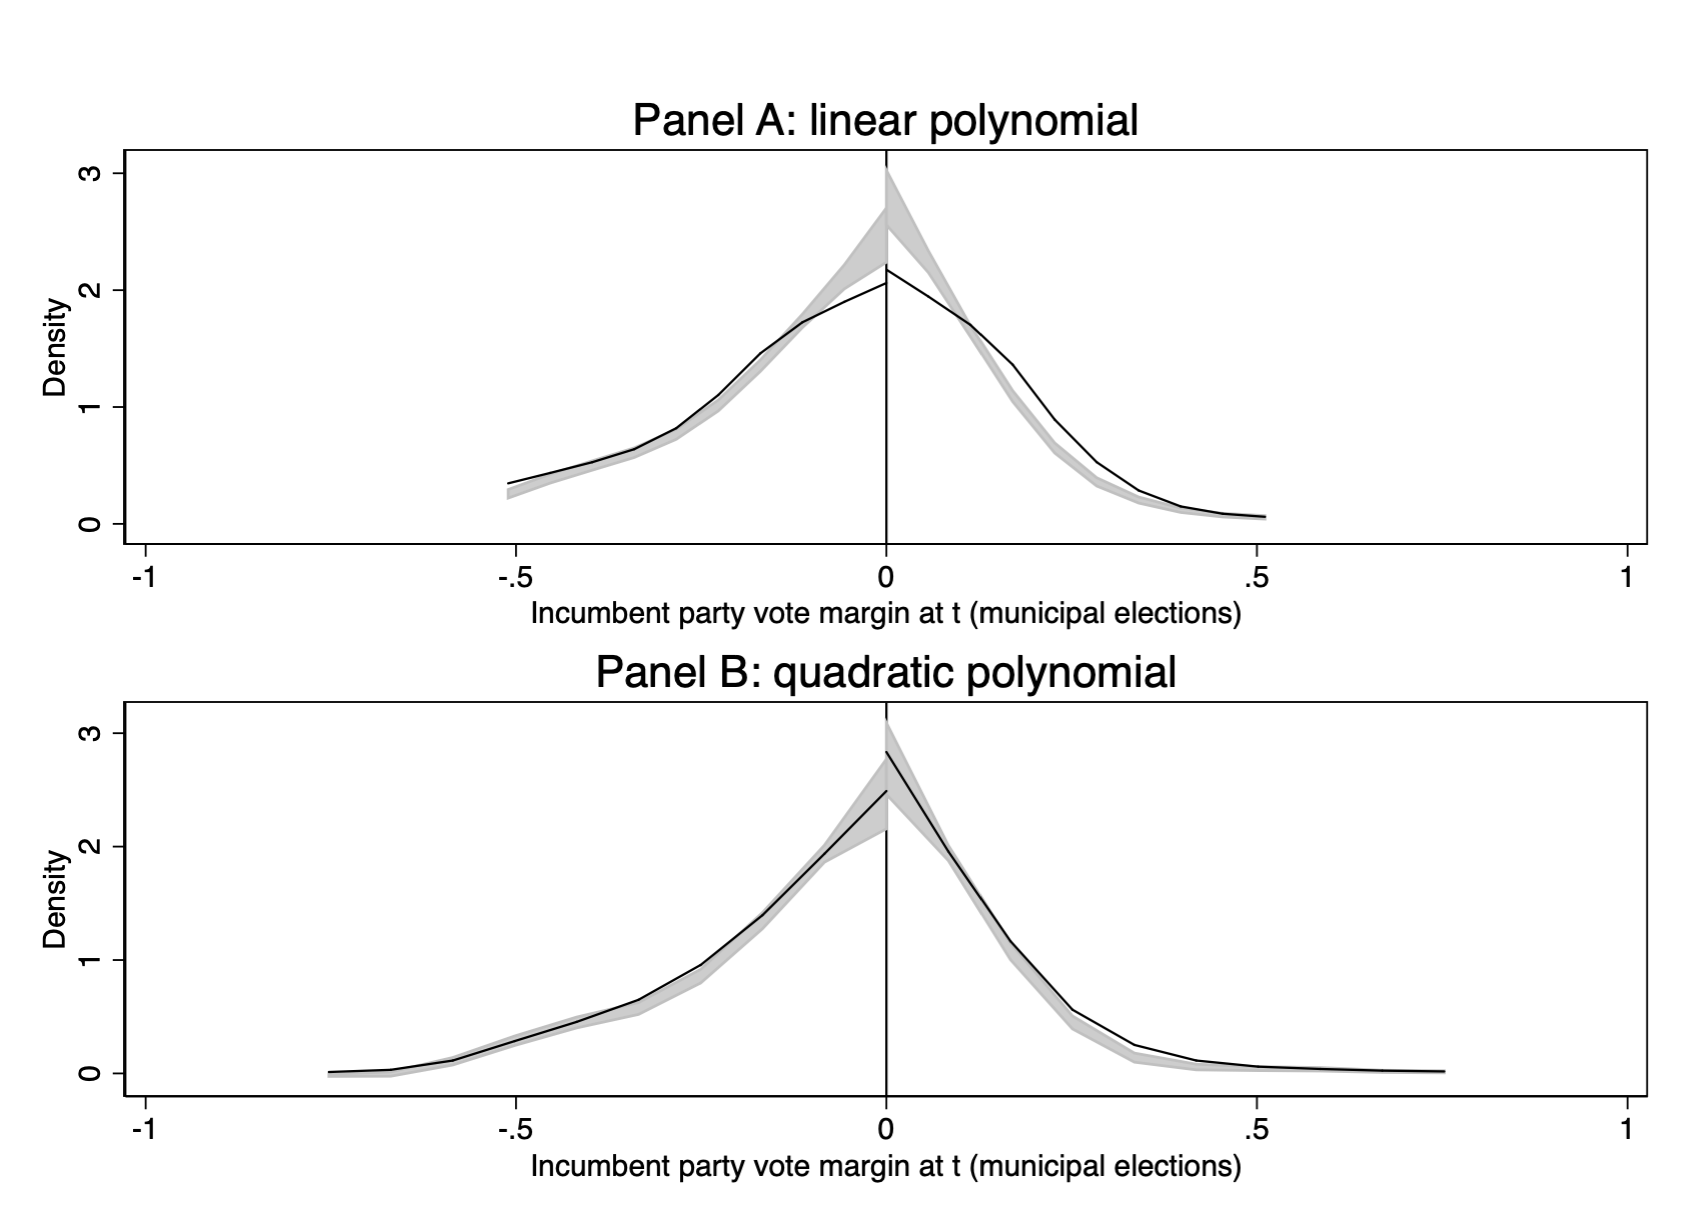
\includegraphics[width=1\textwidth]{Chapter2/Figures_incumbency/mccrary_pol1_2.png}
%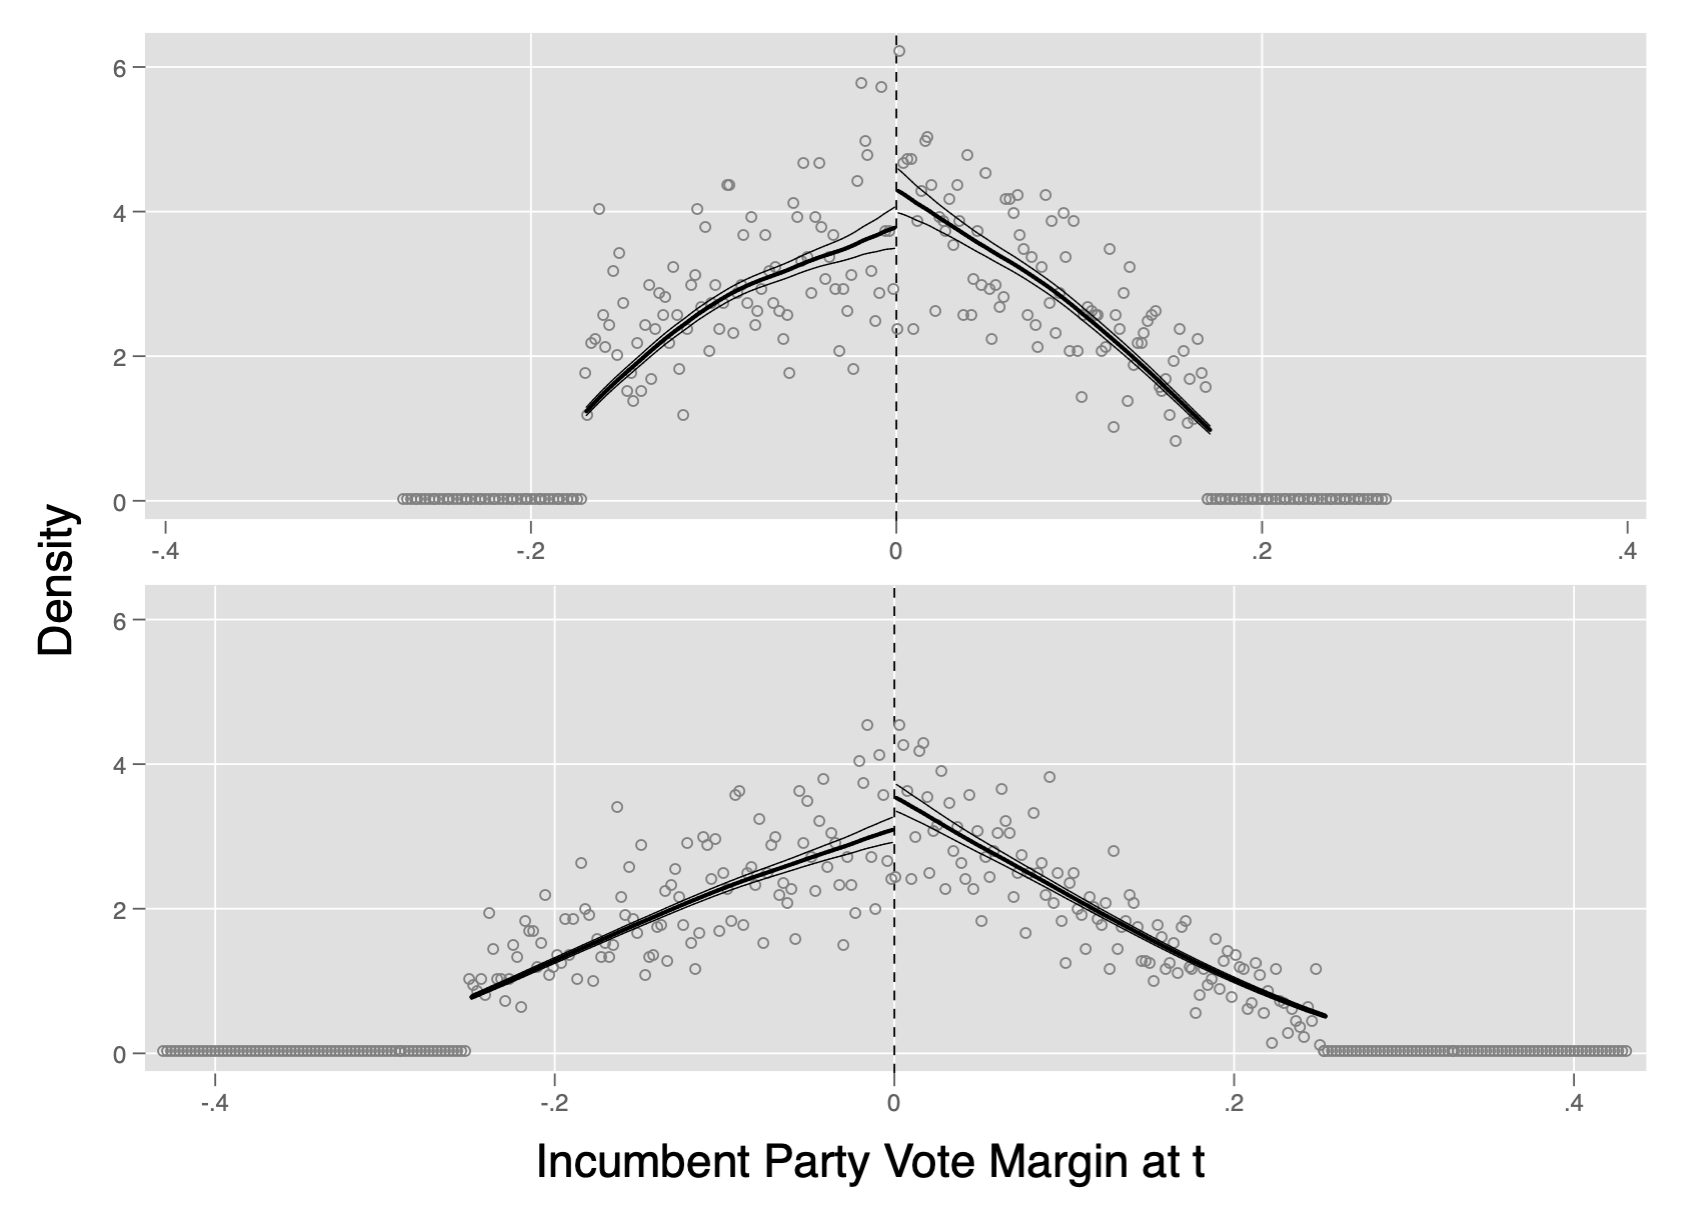
\includegraphics[width=0.9\textwidth]{../Figures/conditional_mccrary_test_pol1_final.png}

       \captionsetup{justification=centering}
         
 \textbf{Note:} 95\% confidence intervals reported.
 
\end{figure} 


 \begin{figure}[h]   
\centering
 \caption{Testing Different Bandwidths}
 \label{fig:bandwidths}
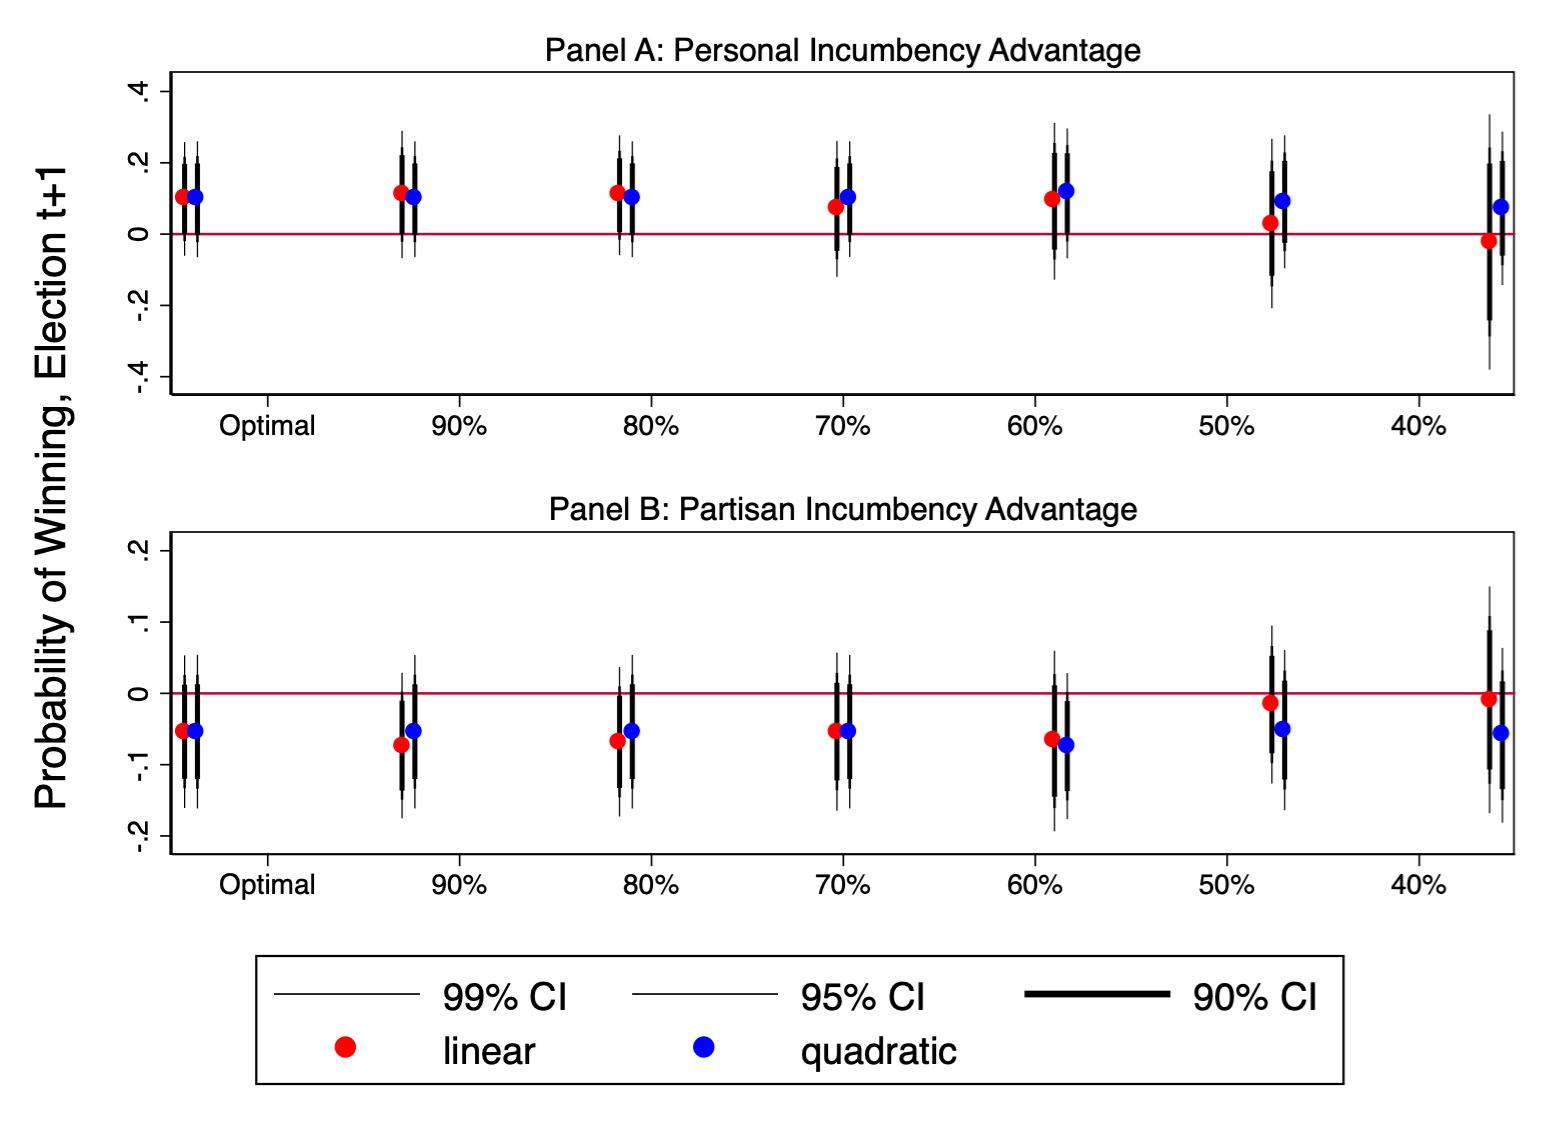
\includegraphics[width=0.65\textwidth]{Chapter2/Figures_incumbency/probability_bandwidths.png}
       \captionsetup{justification=centering}
 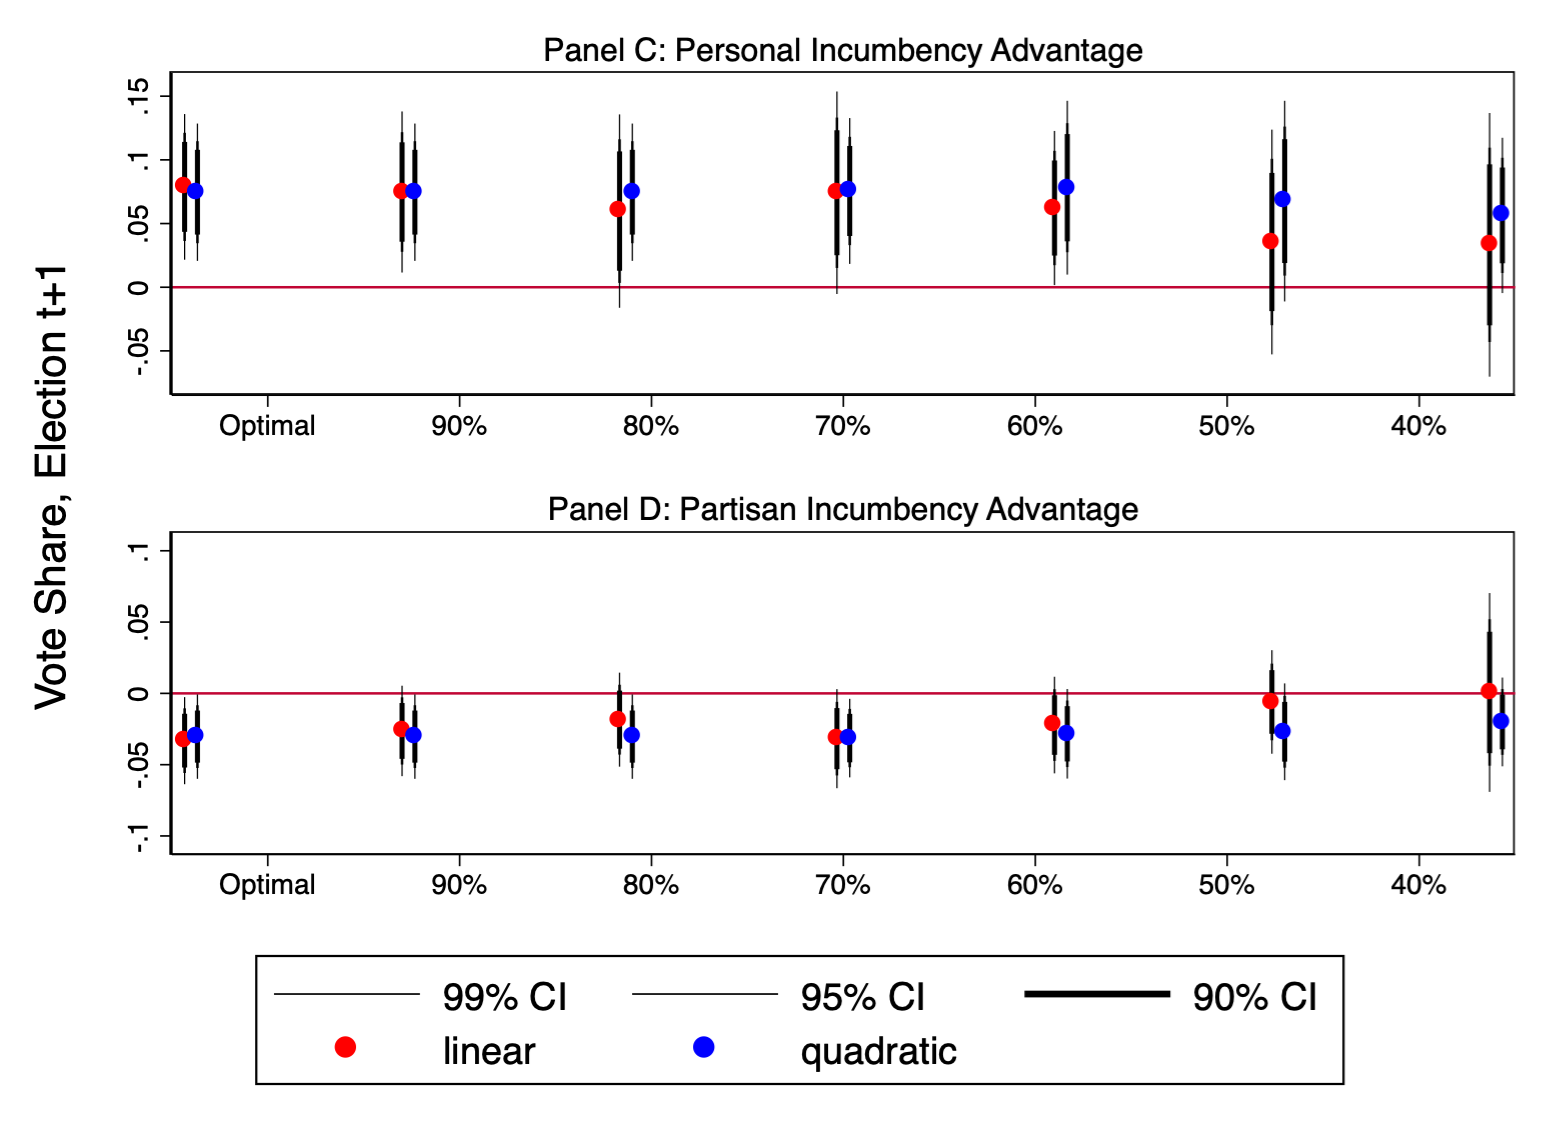
\includegraphics[width=0.65\textwidth]{Chapter2/Figures_incumbency/margin_bandwidths.png}

 \textbf{Note:} Figure \ref{fig:bandwidths} shows the average treatment effect of the Term Limit Reform on the probability of victory in the next election. Various bandwidths are tested as well as the optimal bandwidth following \citet{calonicoetal_2014}. A 90\% implies a reduction of the optimal bandwidth in 10\%, an 80\% a reduction of 20\%, and so on.
   
\end{figure} 
  

%%%% Input bibliography file %%%%%%%%%%%%%%%
% %% NYU PhD thesis format. Created by José Koiller 2007--2008.
%% Updated by Anshul Vikram Pandey with new design guidelines. 2017-2018

%% Use the first of the following lines during production to
%% easily spot "overfull boxes" in the output. Use the second
%% line for the final version.
\documentclass[12pt,draft,letterpaper]{report}
% \documentclass[12pt,letterpaper]{report}
% \documentclass[12pt]{article}

%% Replace the title, name, advisor name, graduation date and dedication below with
%% your own. Graduation months must be January, May or September.
%WILLING STATELESSNESS: THREE ESSAYS ON THE POLITICAL ECONOMY OF LOCAL GOVERNMENTS IN ONGOING CRIMINAL WARS''
\newcommand{\thesistitle}{ESSAYS ON THE POLITICAL ECONOMY OF LOCAL GOVERNMENTS IN ONGOING CRIMINAL WARS}
\newcommand{\thesisauthor}{Rafael J. Ch Duran}
\newcommand{\thesisadvisor}{Pablo Querubin Borrero}
\newcommand{\graddate}{June 2021} % like January XX, May 20XX, September 20XX

%% If you do not want a dedication, scroll down and comment out
%% the appropriate lines in this file.
\newcommand{\thesisdedication}{A mis tres princesas, Mamá, Areli y Lala (juntitos para siempre)}

%% The following makes chapters and sections, but not subsections,
%% appear in the TOC (table of contents). Increase to 2 or 3 to
%% make subsections or subsubsections appear, respectively. It seems
%% to be usual to use the "1" setting, however.
\setcounter{tocdepth}{1}

%% Sectional units up to subsubsections are numbered. To number
%% subsections, but not subsubsections, decrease this counter to 2.
\setcounter{secnumdepth}{3}

% Setting a gap between page number and text block


%% Page layout (customized to letter paper and NYU requirements):
\setlength{\oddsidemargin}{.6in}
\setlength{\textwidth}{5.8in}
\setlength{\topmargin}{0.5in}
\setlength{\headheight}{0in}
\setlength{\headsep}{0in}
\setlength{\textheight}{8.3in}
\setlength{\footskip}{.5in}

%% Use the following commands, if desired, during production.
%% Comment them out for final version.
%\usepackage{layout} % defines the \layout command, see below
%\setlength{\hoffset}{-.75in} % creates a large right margin for notes and \showlabels

      


%%%%%%

%% Controls spacing between lines (\doublespacing, \onehalfspacing, etc.):
\usepackage{setspace}

%
%% \usepackage{amsmath}
%% \usepackage{amssymb}
\usepackage{xspace}
\usepackage{algorithmic}
\usepackage{algorithm}
\usepackage{microtype}
\usepackage{subfigure}
\usepackage{color}
\usepackage{url}
\usepackage{lipsum}
\usepackage{fancyhdr}
% \newfloat{algorithm}{t}{lop}

\pagestyle{fancy}
\fancyhf{}
\renewcommand{\headrulewidth}{0pt}
\fancyhead[LE]{}
\fancyhead[RO]{}
\fancyhead[RE]{}
\fancyhead[LO]{}
\fancyfoot[C]{}
\rhead{\thepage}

\fancypagestyle{plain}{%
\fancyhf{}
\rhead{\thepage}
}

\setlength{\headheight}{20pt} 

%% Use the line below for official NYU version, which requires
%% double line spacing. For all other uses, this is unnecessary,
%% so the line can be commented out.
\onehalfspacing % requires package setspace, invoked above

%% Each of the following lines defines the \com command, which produces
%% a comment (notes for yourself, for instance) in the output file.
%% Example:    \com{this will appear as a comment in the output}
%% Choose (uncomment) only one of the three forms:
%\newcommand{\com}[1]{[/// {#1} ///]}       % between [/// and ///].
\newcommand{\com}[1]{\marginpar{\tiny #1}} % as (tiny) margin notes
%\newcommand{\com}[1]{}                     % suppress all comments.

%% This inputs your auxiliary file with \usepackage's and \newcommand's:
%% It is assumed that that file is called "definitions.tex".
%%
%% Place here your \usepackage's. Some recommended packages are already included.
%%

% Graphics:
\usepackage[final]{graphicx}
%\usepackage{graphicx} % use this line instead of the above to suppress graphics in draft copies
%\usepackage{graphpap} % \defines the \graphpaper command

% Indent first line of each section:
\usepackage{indentfirst}

% Good AMS stuff:
\usepackage{amsthm} % facilities for theorem-like environments
\usepackage[tbtags]{amsmath} % a lot of good stuff!

% Fonts and symbols:
\usepackage{amsfonts}
\usepackage{amssymb}

\usepackage{xspace}
\usepackage{algorithmic}
\usepackage{algorithm}
\usepackage{microtype}
\usepackage{subfigure}
\usepackage{color}
\usepackage{todonotes}
\usepackage{url}
\newfloat{algorithm}{t}{lop}

% Formatting tools:
%\usepackage{relsize} % relative font size selection, provides commands \textsmalle, \textlarger
%\usepackage{xspace} % gentle spacing in macros, such as \newcommand{\acims}{\textsc{acim}s\xspace}

% Page formatting utility:
\usepackage{geometry}
\usepackage{multirow}
\usepackage{listings}
%
\usepackage[round,authoryear]{natbib}
\usepackage[all,cmtip]{xy}
\usepackage[colorlinks=true,citecolor=blue,urlcolor=blue, filecolor=blue,pdfpagemode=UseNone,pdfstartview=FitH, final]{hyperref}
%\usepackage[breaklinks=true,a4paper=true,pagebackref=true]{hyperref}
\usepackage{tocloft}
\newcommand{\Color}[1]{\hypersetup{linkcolor=#1}\color{#1}}
\renewcommand{\cftchapfont}{\Color{black}\large\bfseries}
\renewcommand{\cftsecfont}{\Color{black}}
\renewcommand{\cftsubsecfont}{\Color{black}}
\renewcommand{\cftsubsubsecfont}{\Color{black}}
\renewcommand{\cftchappagefont}{\Color{black}}
\renewcommand{\cftsecpagefont}{\Color{black}}
\renewcommand{\cftsubsecpagefont}{\Color{black}}
\renewcommand{\cftsubsubsecpagefont}{\Color{black}}
\renewcommand{\cftsecleader}{\Color{black}\cftdotfill{\cftsecdotsep}}
\renewcommand{\cftsubsecleader}{\Color{black}\cftdotfill{\cftsubsecdotsep}}
\renewcommand{\cftsubsubsecleader}{\Color{black}\cftdotfill{\cftsubsubsecdotsep}}
\renewcommand{\cftchapleader}{\large\bfseries\color{black}\cftdotfill{\cftdotsep}}
\renewcommand{\cftchappagefont}{\large\bfseries}
%\usepackage{hyperref}
%\hypersetup{
 %   colorlinks=true,
  %  linkcolor=blue,
   % filecolor=blue,
%    urlcolor=blue,
 %    citecolor=blue
 % }

%%
%% Place here your \newcommand's and \renewcommand's. Some examples already included.
%%
%\newcommand{\acims}{\textsc{acim}s\xspace}
\newcommand{\Mspace}        {{\mathbb M}}
\newcommand{\Rspace}        {{\mathbb R}}
\newcommand{\Cspace}        {{\mathbb C}}

\newcommand{\Mo}        {{\hat M}}
\newcommand{\Ms}        {{\tilde M}}
\newcommand{\Do}          {{\hat D}}
\newcommand{\Ds}        {{\tilde D}}
\newcommand{\doo}          {{\hat d}}
\newcommand{\dss}        {{\tilde d}}
\newcommand{\w}        {{\mathbf w}}

% general
\newcommand{\ie}{i.e.}
\newcommand{\eg}{e.g.}
\newcommand{\reffig}[1]{{Figure~\ref{#1}}}
\newcommand{\refchap}[1]{{Chapter~\ref{#1}}}
\newcommand{\refsec}[1]{{Section~\ref{#1}}}
\newcommand{\reftab}[1]{{Table~\ref{#1}}}
\newcommand{\refapp}[1]{{Appendix~\ref{#1}}}
\newcommand{\refeq}[1]{{Equation~\ref{#1}}}
\newcommand{\refalg}[1]{{Algorithm~\ref{#1}}}
\newcommand{\myparagraph}[1]{\noindent \textbf{#1}}
\newcommand{\highlight}[1]{{\color{black}#1}}


%%%%RAFA PACKAGES
\usepackage[font=bf, justification=centering]{caption}
\DeclareUnicodeCharacter{00A0}{'}
\usepackage{longtable}    
\usepackage{lscape}
\usepackage{booktabs}
%\usepackage[colorlinks=true,citecolor=blue,urlcolor=blue,pdfpagemode=UseNone,pdfstartview=FitH]{hyperref}

%%
%% Place here your \newtheorem's:
%%

%% Some examples commented out below. Create your own or use these...
%%%%%%%%%\swapnumbers % this makes the numbers appear before the statement name.
%\theoremstyle{plain}
%\newtheorem{thm}{Theorem}[chapter]
%\newtheorem{prop}[thm]{Proposition}
%\newtheorem{lemma}[thm]{Lemma}
%\newtheorem{cor}[thm]{Corollary}

%\theoremstyle{definition}
%\newtheorem{define}{Definition}[chapter]

%\theoremstyle{remark}
%\newtheorem*{rmk*}{Remark}
%\newtheorem*{rmks*}{Remarks}

%% This defines the "proo" environment, which is the same as proof, but
%% with "Proof:" instead of "Proof.". I prefer the former.
%\newenvironment{proo}{\begin{proof}[Proof:]}{\end{proof}}


%% Cross-referencing utilities. Use one or the other--whichever you prefer--
%% but comment out both lines for final version.
%\usepackage{showlabels}
%\usepackage{showkeys}
% \pagestyle{headings}

\begin{document}
%% Produces a test "layout" page, for "debugging" purposes only.
%% Comment out for final version.
%\layout % requires package layout (see above, on this same file)
%% Sets page numbering to "roman style" i, ii, iii, iv, etc:

%%%%%% Cover page %%%%%%%%%%%
%% Sets page numbering to "roman style" i, ii, iii, iv, etc:
\pagenumbering{roman}
\thispagestyle{empty}
\begin{center}
{\bfseries 
  {\large\thesistitle}
  \vspace{1in}
  
 {\large {\bf DISSERTATION}}\\
  \vspace{.3in}
  
  \begin{doublespace}
  {\large  
  Submitted in Partial Fulfillment of\\
  % \vspace{.1in}
  the Requirements for\\
  % \vspace{.1in}
  the Degree of\\}
  \end{doublespace}
  \vspace{.3in}
  
  {\large DOCTOR OF PHILOSOPHY \\ (Political Science)}\\
  \vspace{.5in}
  
  at the \\
  \vspace{.2in}
  
  {\large
  NEW YORK UNIVERSITY\\
  \vspace{-0.05in}
  GRADUATE SCHOOL OF ARTS AND SCIENCE\\
  }
  \vspace{.2in}
  
  by
  \vspace{.5in}

  {\large\thesisauthor}
  \vspace{.5in}
  % \vfill

  {\large\graddate}
}

\end{center}

\newpage

%%%%%% Title page %%%%%%%%%%%
%
\setcounter{page}{1}
%% No numbering in the title page:
\thispagestyle{empty}
%
\begin{center}
{\bfseries 
  {\large\thesistitle}
  \vspace{.2in}
  
  DISSERTATION\\
  \vspace{.2in}
  
  \begin{doublespace}
  Submitted in Partial Fulfillment of\\
  % \vspace{.1in}
  the Requirements for\\
  % \vspace{.1in}
  the Degree of\\
  \end{doublespace}
  \vspace{.2in}
  
  DOCTOR OF PHILOSOPHY  (Political Science)\\
  \vspace{.2in}
  
  at the \\
  \vspace{.1in}
  
  {\large
  NEW YORK UNIVERSITY\\
  \vspace{-0.05in}
  GRADUATE SCHOOL OF ARTS AND SCIENCE\\
  }
  \vspace{.1in}
  
  by
  \vspace{.15in}

  \thesisauthor
  \vspace{.15in}
  % \vfill

  \graddate
}

\end{center}
% \vfill

\vspace{0.2in}

\noindent
\makebox[\textwidth]{\hfill\makebox[2.5in]{Approved: \hfill}}
\vspace{0.1in}

\noindent
\makebox[\textwidth]{\hfill\makebox[2.5in]{\hrulefill}}\\
\makebox[\textwidth]{\hfill\makebox[2.5in]{\hfill Department Chair Signature\hfill}}
\vspace{0.05in}

\noindent
\makebox[\textwidth]{\hfill\makebox[2.5in]{\hrulefill}}\\
\makebox[\textwidth]{\hfill\makebox[2.5in]{\hfill Date \hfill}}

\noindent
University ID: {N16628197}\\ % Add your University ID
Net ID: \hspace{.415in} {rcd306}\\ % Add your Net ID
\break
%\newpage

%%%%%%%%%%%%%% Copyright Page %%%%%%%%%%%%%%%%%

%%%%%%%%%%%%%% Guidance Committee Signature Page %%%%%%%%%%%%%%%%%
\singlespacing
\noindent
Approved by the Guidance Committee: \\
\underline{Major}: Political Science
%\vspace{0.01in}

\noindent
\makebox[\textwidth]{\hfill\makebox[3in]{\hrulefill}}\\
\makebox[\textwidth]{\hfill\makebox[3in]{\hfill \textbf{Pablo Querubin Borrero}\hfill}}
\makebox[\textwidth]{\hfill\makebox[3in]{\hfill Associate Professor of \hfill}}
\makebox[\textwidth]{\hfill\makebox[3in]{\hfill Politics and Economics at NYU \hfill}}
\makebox[\textwidth]{\hfill\makebox[3in]{\rule[-4pt]{2in}{1pt}}}\\
\makebox[\textwidth]{\hfill\makebox[3in]{\hfill June 24, 2021 \hfill}}\\
\vspace{0.1in}
\noindent
\makebox[\textwidth]{\hfill\makebox[3in]{\hrulefill}}\\
\makebox[\textwidth]{\hfill\makebox[3in]{\hfill \textbf{Cyrus Samii}\hfill}}
\makebox[\textwidth]{\hfill\makebox[3in]{\hfill Associate Professor of \hfill}}
\makebox[\textwidth]{\hfill\makebox[3in]{\hfill Politics at NYU \hfill}}
\makebox[\textwidth]{\hfill\makebox[3in]{\rule[-4pt]{2in}{1pt}}}\\
\makebox[\textwidth]{\hfill\makebox[3in]{\hfill June 24, 2021 \hfill}}\\
\vspace{0.1in}
\noindent
\makebox[\textwidth]{\hfill\makebox[3in]{\hrulefill}}\\
\makebox[\textwidth]{\hfill\makebox[3in]{\hfill \textbf{Hye Young You}\hfill}}
\makebox[\textwidth]{\hfill\makebox[3in]{\hfill Assistant Professor of \hfill}}
\makebox[\textwidth]{\hfill\makebox[3in]{\hfill Politics at NYU \hfill}}
\makebox[\textwidth]{\hfill\makebox[3in]{\rule[-4pt]{2in}{1pt}}}\\
\makebox[\textwidth]{\hfill\makebox[3in]{\hfill June 24, 2021 \hfill}}\\
\vspace{0.1in}
\noindent
\makebox[\textwidth]{\hfill\makebox[3in]{\hrulefill}}\\
\makebox[\textwidth]{\hfill\makebox[3in]{\hfill \textbf{Tara Slough}\hfill}}
\makebox[\textwidth]{\hfill\makebox[3in]{\hfill Assistant Professor of \hfill}}
\makebox[\textwidth]{\hfill\makebox[3in]{\hfill Politics at NYU \hfill}}
\makebox[\textwidth]{\hfill\makebox[3in]{\rule[-4pt]{2in}{1pt}}}\\
\makebox[\textwidth]{\hfill\makebox[3in]{\hfill June 24, 2021 \hfill}}\\
\vspace{0.1in}
\noindent
\makebox[\textwidth]{\hfill\makebox[3in]{\hrulefill}}\\
\makebox[\textwidth]{\hfill\makebox[3in]{\hfill \textbf{Juan F. Vargas}\hfill}}
\makebox[\textwidth]{\hfill\makebox[3in]{\hfill Professor of \hfill}}
\makebox[\textwidth]{\hfill\makebox[3in]{\hfill Economics at Universidad El Rosario \hfill}}
\makebox[\textwidth]{\hfill\makebox[3in]{\rule[-4pt]{2in}{1pt}}}\\
\makebox[\textwidth]{\hfill\makebox[3in]{\hfill June 24, 2021 \hfill}}\\

\doublespacing

%%%%%%%%%%%%%% Microfilm / Publishing Page %%%%%%%%%%%%%%%%%
\break
\begin{center}
\copyright  by Rafael J. Ch Durán, 2021. All rights reserved.

%Microfilm or other copies of this dissertation are obtainable from
%\vspace{4in}

%UMI Dissertation Publishing\\
%ProQuest CSA\\
%789 E. Eisenhower Parkway\\
%P.O. Box 1346\\
%Ann Arbor, MI 48106-1346

\end{center}
\newpage

%%%%%%%%%%%%%% Vita %%%%%%%%%%%%%%%%%
\section*{Vita}
\addcontentsline{toc}{section}{Vita}
%!TEX root = thesis.tex

I’m a Ph.D. Candidate in the Politics Department at New York University. My research interests lie in Comparative Politics and Methods, and include the study of Governance, Conflict, and State Capture. I have a regional specialization in developing countries, particularly Latin America.

I received NYU’s Dean’s Dissertation Fellowship 2020-2021. My research has also been supported by organizations including the Fulbright-Garcia Robles Program, the Development Bank of Latin America (CAF), the Center for Studies in Security and Drugs (CESED) from Universidad Los Andes, among others. My scholarly work has been published in the American Political Science Review, the Journal of Urban Economics and I have been a referee for the American Political Science Review, Comparative Political Studies, and Latin American Research Review.

While in the Ph.D. program at NYU, I also served as Principal Investigator for the Latin America Development Bank´s (CAF) “Slum Observatory” Project, and worked on CAF’s leading chapter of the flagship annual Economy and Development Report 2017 on Urban Development in Latin America. In 2015 I served as a Research Assistant at the Empirical Studies of Conflict (ESOC) at Princeton University. Prior to NYU, I served as Director of the Economic and Public Security Research Division at the Center of Research for Development, A.C. (CIDAC), and as a Visiting Professor at the Political Science Department of the Instituto Tecnológico Autónomo de México (ITAM) where I thought Political Methodology. I received my BA in Economics from ITAM with the highest distinction. 

\newpage



%%%%%%%%%%%%%% Ackknowlegment %%%%%%%%%%%%%%%%%
%% Comment out the following lines if you do not want to acknowledge
%% anyone's help...
\section*{Acknowledgements}
\addcontentsline{toc}{section}{Acknowledgements}
%!TEX root = thesis.tex

%% Write your acknowledgements in this file. If you do not want to acknowledge anyone,
%% you can delete this file and comment out the corresponding part in the "thesis.tex"
%% file.


This dissertation is the result of multiple years of work and the involvement of many people. There are no words to express the gratitude and appreciation to every single person that supported me throughout the last 7 years at NYU. Thanks to all of you, I finish this stage in life with a heart filled with joy and hope for things to come. 

First and foremost, I want to thank my dissertation committee. Pablo Querubin, thank you for believing in me since we first met, for giving me the opportunity to teach side-by-side with you for five years, for always being patient with me, for spending countless hours to talk about my research and even job opportunities, for always doing so with a big smile. Thank you for your advice inside and outside the classroom, for leading me to new research opportunities, for pushing my research, for being my mentor and friend. I will never forget the words you gave to the Latin American Politics class in the last lecture of Spring of 2017: you spoke of how the class revolved around portraying the faults of Latin America but that students should not loose sight of the beauties of the region, and the promise of hope for it. Your love for Latin America is something I will carry on for the rest of my life. Cyrus Samii, there is no way I can express how much I thank you for all your support these years. There were times in the Ph.D. program where I thought I couldn't make it but it was your advice and guidance throughout these years that help me build confidence in my research. I will never forget the days spend in Morocco, your help to meet new faculty members, your methodological teaching, your mentoring and support. Hye Young You, the first time I met you, you had read all of my work in such a thorough way that left me amazed. Your insights and clarity have been extremely helpful, and much of what I could do in this dissertation was thanks to those meetings with you. If the kindness and patience you have showed to me was present in every faculty member, academia would be the best of places in the world. Tara Slough, as I have told you before, every time I see you participate in a seminar, deliver comments to students or in conferences, and when you have spoken directly to my research you have always provided the best of feedback. I have long admired your research and work ethic. Begin honest, I wish I could be like you, and I'm so happy to have you as part of my committee. Juan Vargas, mi mentor y mi amigo, if there is someone to truly thank throughout all these years is you. Since the Summer of 2015 you opened your arms to me as a collegue, and few days after as friend for life. There is no one I have learned from as you, who truly built up my foundations as a researcher, who opened up research opportunities to me that I would have never dreamed about. 

I also want to thank the faculty members at NYU and Princeton University. Neal Beck, there is no man in academia like you, there is no one that loves students as you do. It is becasue of you that a boy in a Masters program with hopes of joining a Ph.D. program achieved his dream as is now about to finish it. I will be eternally grateful for your support and friendship. Jake Shapiro, I met you at the end of my first year at the Masters at NYU. Since then my life changed and I couldn't even imagine everything that happened since, and much of it was due to your mentoring, support, and friendship. You are a dreambuilder, and I have achieved many of my dreams by being under your wing. I'm truly thankful to you and excited for the work to come in the following years. Leonard Wantchekon, thank you for sharing some of your passion for research and how to better the world we are living in. Your trust in me and all the research opportunities you have shared with me cannot be repaid.

Thank you for all the faculty members at NYU that shared their knowledge and advice during my doctoral studies. Thank you Dimitri Landa, Peter Rosendorff, Shanker Satyanath, Nicole Simonelli,  Amanda Kennard, Tiberiu Dragu, Mike Gilligan, David Stasavage, and Julia Payson.  

God has given me the best friends: I am truly the happiest man of the world because of you. Gordos, Gabriel y Gizeh, mis amigos del alma, los tres mosqueteros hasta el final, verdaderamente me han enseñado que el hierro con hierro se afila. Alan, el hermano que nunca tuve y que me ha acompañado hasta este día. Si en alguien dejara mi vida sería en tus manos. Así como tus logros son mis logros, espero \'este sea uno tuyo pues no pude haberlo alcanzado sin tu amistad. Andresiño -my fish!- y Juanda, mis dos hermanos de otros padres, dos regalos que Dios me dió de pura gracia y que serán mi familia por siempre. Nick, I never thought to find a friend like you in the States, and to admire a man the way I admire you. You are one of God's best gifts I have in my life. I have missed you since you left NYC. Prabin, your heart is the biggest of all, and your friendship a true gift. To both of you, Nick and Prabin, I couldn´t have done the Ph.D. without you, you were the greatest support, and the truest of friends. Reed, I wish we could have met earlier in the progam but I thank God for that trip to China, for the endless talks we have had since, for your friendship, your guidance and mentoring. We are brothers for life. To all my friends at NYU, thank you: Will, Antonella, Mateo, Mariana, Dongil, Abraham, Felipe, Martin, Patrick, Arina, Maria, Anne, Giacomo, Athena, Rajeshwari, Lucia, Ye, and Stephanie.

To my friends in NYC, thank you for being present throughout these years, for all your prayers and support. Rich, my dear friend and brother, you have been and advisor and the best of friends. Truly, you have showed me that there is a friend that is closer than a brother. Jing, there is no day that I miss you in NY. God blessed me with your life since we met. To all the members of the Stuy CG and Redeemer, Fei Mei, Sam, Melody, Miguelo, Emilia, Diane, Becks, Audrey, and many, many more. To all of you and even the ones I don't name, thank you for your frienship and your love. You are my NYC family, and there is no better family than you all. 

To my students from the IR Honors, Latin American Politics, and Political Economy of Development classes at NYU, thank you. Back when I was living in Mexico and before coming to the States I had a dream of becoming an advisor to kings and queens. For years I thought I would achieve that by taking a job in public office. You, however, thought me that by teaching I was already fulfilling the biggest dream in my heart. You, my kings and queens, are my joy and glory. 

Finally, and most importantly, I'm grateful to my family. Mamá eres a quien más admiro en el mundo y cuyo amor me sostuvo todos estos años: mi gran consejera y mi gran amiga. Arela y Lala, mis amores, mis hermanitas hermosas que con su amor me apoyaron día tras día, y me hacen querer ser mejor cada día. A las tres sepan que mis sueños cumplidos son suyos, mis logros sus logros, mi honor su honor, pues no hay nada que que hubiera logrado sin ustedes. Su amor es mi motor y el regalo más grande de Dios en esta vida. Esta disertación se las dedico a ustedes. Las amo.

God, I have fought the good fight, I have finished the race, I have kept the faith. You have lifted my head up high, you have sustained me and loved me like nobody has. My life is yours, this degree is yours, and to you, who is able to do immesurably more than all we ask or imagine, to you God be the glory forever and ever. 

\noindent
\makebox[\textwidth]{\hfill\makebox[3in]{\hfill Rafael J. Ch Duran\hfill}}
\makebox[\textwidth]{\hfill\makebox[3in]{\hfill\graddate\hfill}}


\newpage

%%%%%%%%%%%%%% Dedication Page %%%%%%%%%%%%%%%%%
%% Comment out the following lines if you do not want to dedicate
%% this to anyone...
\vspace*{\fill}
\begin{center}
  \thesisdedication%\addcontentsline{toc}{section}{Dedication}
\end{center}
\vfill
\newpage


%%%%%%%%%%%%%% Abstract %%%%%%%%%%%%%%%%%
\section*{}
\begin{center}
{\bfseries 
  %{\large\thesistitle}
  \vspace{.25in}  
  {\bf ABSTRACT}\\
  \vspace{.25in}
  {\bf \thesistitle}\\  
  \vspace{.25in}
  {\bf by}\\  
  \vspace{.5in}
  {\bf \thesisauthor}\\
  \vspace{.5in}
  {\bf Advisor: Prof. \thesisadvisor, Ph.D.}\\
  \vspace{.25in}
  {\bf Submitted in Partial Fulfillment of the Requirements for}\\
  {\bf the Degree of Doctor of Philosophy (Political Science)}\\
  \vspace{.25in}
  {\bf \graddate}  
  \vspace{.25in}
}
\end{center}
\addcontentsline{toc}{section}{Abstract}
%!TEX root = thesis.tex

This dissertation studies what prevents (or fosters) would-be contemporary nation-builders from building the nation and solidifying the state when challenged by criminal wars. Focusing on Mexico and Colombia -two states rampaged by ongoing criminal wars-, I study the incentives of local governments electoral incentives (Chapter 1 and 2), and the way in which non-state armed groups capture them and transform local institutions to their preferences (Chapter 3). 

The first chapter titled ``Reelection Backfire: How Reelection Concerns Affect the Delegation of Public Security Policy in Mexico'' studies the effect of reelection incentives of mayors on the delegation of security policy to governors in Mexico. It is no easy task for local governments to combat organized crime and hold the monopoly of violence. Faced by resource, expertise, or information constraints, or in the presence of large spillovers, mayors may choose to delegate security policy to more efficient agents like the governor or the president. However, by doing so mayors loose the use of security policy for electoral purposes: they cannot longer claim competence and willingness to fight crime or be responsive to citizens demands. A clear tradeoff between efficiency and electoral incentives arises. This paper studies the effect of mayors' reelection incentives on the delegation of security policy to the governor in a country overwhelmed by criminal wars, Mexico. To do so, I leverage the staggered implementation of an electoral reform that introduced reelection for mayors from 2014 to 2022. I find that mayors up for reelection decrease the delegation of public security to the governor of their state relative to term-limited mayors. By taking charge of policy, mayors facing reelection differentiate themselves from other political actors believing this would increase their reelection chances. However, no evidence is found that mayors increase their effort to fight crime and address citizens security concerns. The consequence of not delegating to more efficient actors, however, is an increase in violence. This paper suggests that delegation is not only a policy decision but an electoral one, and that reelection incentives may lead incumbents to differentiate themselves by taking charge of public policy at the expense of efficiency.   

The second chapter titled ``Love the Candidate but Hate his Party: The Asymmetric Effects of Reelection Incentives on Partisan and Personal Incumbency Returns in Mexico'' studies incumbency returns to office in local governments. A large literature has studied the electoral returns to incumbency. However, the estimated incumbency returns in the majority of studies confound the returns to the incumbent party and politician. As a result we may hold a misguided picture of the relationship between parties and their members, citizens valuation of the electoral system, and the existent electoral accountability. This paper opens up the black box of incumbency by disentangling the personal and partisan incumbency advantages. To do so, I use a difference-in-discontinuity of close elections design in Mexico that exploits the staggered implementation of an electoral reform that introduced reelection for mayors from 2014 to 2022. Term limit elections allow us to identify a partisan advantage since the politician cannot run for office again but his party can. Elections with candidates up for reelection identify both the partisan and personal incumbency returns.  The difference between this two quantities -or the difference-in-discontinuity estimator- identifies the personal from the partisan effect. The main result shows that incumbent politicians up for reelection enjoyed and electoral \emph{advantage}. Contrastingly, incumbent parties in term limit races suffer from an incumbency \emph{disadvantage}. The research design allows to solve several methodological issues of past studies that have tried to disentangle the partisan from the personal effect, primarily rule out potential pretrends of term limit and non-term limit races, as well as concerns on selection coming from the ability and experience of candidates. Overall, the results suggest the personal advantage to be a driving force of incumbency returns, and how  reelection may lead to party dealignment in party-centered systems like Mexico. 

Lastly, the third chapter titled ``Endogenous taxation in ongoing internal conflict: The case of Colombia'' studies how non-state armed groups capture municipalities and transform local institutions according to their preferences. Recent empirical evidence suggests an ambiguous relationship between internal conflicts, state capacity and tax performance. In theory, internal conflict should create strong incentives for governments to develop the fiscal capacity necessary to defeat rivals. In this chapter we argue that one reason that this does not occur is because internal conflict enables groups with {\it{de facto}} power to capture local fiscal and property rights institutions. We test this mechanism in Colombia using data on tax performance and property rights institutions at the municipal level. Municipalities affected by internal conflict have tax institutions consistent with the preferences of the parties dominating local violence. Those suffering more right-wing violence feature more land formalization and higher property tax revenues. Municipalities with substantial left-wing guerrilla violence collect less tax revenue and witness less land formalization. Our findings provide systematic evidence that internal armed conflict helps interest groups capture municipal institutions for their own private benefit, impeding state-building.


\newpage

%%%% Table of Contents %%%%%%%%%%%%
\tableofcontents
% \clearpage
% \pagestyle{headings}

%%%%% List of Figures %%%%%%%%%%%%%
%% Comment out the following two lines if your thesis does not
%% contain any figures. The list of figures contains only
%% those figures included withing the "figure" environment.
\listoffigures\addcontentsline{toc}{section}{\listfigurename}
\newpage

%%%%% List of Tables %%%%%%%%%%%%%
%% Comment out the following two lines if your thesis does not
%% contain any tables. The list of tables contains only
%% those tables included withing the "table" environment.
\listoftables\addcontentsline{toc}{section}{\listtablename}
\newpage

%%%%% Body of thesis starts %%%%%%%%%%%%
\pagenumbering{arabic} % switches page numbering to arabic: 1, 2, 3, etc.

%% Introduction. If your thesis has no introduction, or chapter 1 is
%% meant to be the introduction, then comment out the lines below.
%% \section*{Introduction}\addcontentsline{toc}{section}{Introduction}
%\input{intro}

%%If your thesis has different "Parts", use commands such as the following:

\section{Introduction}
      
                    
Normatively, efficiency and equity considerations should determine which level of government takes charge of policy and public good delivery \citep{oates_1972, Musgrave_1959, Musgrave_1983, gramlich_1977}. In some cases, however, certain levels of government may hold the responsibility of policymaking despite being the least efficient to do so due to constraints on resources \citep{Moravcsik_2000}, expertise or information \citep{Rodrick_1996} or the existence of spillovers \citep{oates_1972,  Besley_case_1995}. This is the case of the monopoly of violence in conflict settings where subnational units might not be able to fight non-state armed groups: they may be more prone to capture, coercion and strife \citep{chacon_2018}, and their fight against crime might only create a ``balloon effect’’ where criminal organizations simply move to nearby localities where crime is less well clamped down \citep{shirk_wallman_2015}. Unable to deliver security policy efficiently, subnational governments may choose to delegate it to upper-level governments who can pool resources, gather better information, develop economies of scale and specialize \citep{Hawkins_etal_2006}, and combat crime more efficiently. By delegating, however, incumbents lose the capacity to use policy as an instrument to gather votes: they cannot send a signal to voters on competence and being strong types to battle crime, and they cannot be responsive to voters demands, weakening the electoral accountability created by reelection \citep{cox_katz_2002}. A clear tradeoff between efficiency and electoral incentives arises.    
     
In this paper, I study the extent to which reelection incentives shape the delegation of security policy. I argue that compared to term limit incumbents who hold no interest of impressing voters \citep{ashworth_2012}, incumbents eligible for reelection take charge of security policy to signal competence and a strong type to voters to differentiate themselves from other political actors and increase their reelection chances.  To do so, I study the effect of mayors' reelection incentives on the delegation decision of public security policy to the governor in a country overwhelmed by criminal wars, Mexico \citep{ley_trejo_2020}.\footnote{Prior to the COVID-19 crisis, public insecurity in Mexico was the principal public problem as measured by survey data. See \url{https://www.dropbox.com/s/c5dte5pscggat2c/leadingproblem_mexico.png?dl=0} for an example.} According to the Mexican constitution, public security policy falls under the responsibility of mayors. However, since the presidency of Felipe Calderon (PAN, 2006-2012), the Federal government pushed forth the creation of state-level centralized commands where governors could take charge of all security policy within their state.\footnote{This delegation instrument contrasts to simple security cooperation agreements where mayors share security policy responsibilities with governors or other actors. In other words, signing a centralized command agreement implies the delegation of security policy and no cooperation between actors, while simple security cooperation agreements imply a mix of delegation and cooperation.} Mayors face a delegation dilemma: they could sign the centralization command agreement and delegate security policy to a more efficient agent, the governor, or choose to continue take charge of security policy to claim competence and increase their reelection chances. This decision could be made in a yearly basis, and by 2018, 79.12\% of municipalities in the country have delegated security policy to the governor at least one year since 2010.\footnote{According to data from the 2019 National Census of Municipal Governments and Territories of the City of Mexico.} 
          
To empirically test the effect of mayors´ reelection incentives on the delegation of security policy to the governor, I use an event-study design that leverages the 2014 Electoral Reform of Mexico that introduced for the first time reelection for mayors for up to 2 consecutive periods. The Electoral Reform, approved in February 2014, was part of the Mexican Pact Accord, a set of structural reforms negotiated by the three main political parties in Mexico at the time (PRI, PAN and PRD). The Electoral Reform was staggered at the state level which allows us to compare the security policy delegation choice of mayors facing term limits -and not-yet-treated- to mayors up for reelection. The difference between these two quantities represents the likelihood of mayors signing centralization agreements (delegation) due to reelection incentives. 
          
Results show that mayors up for reelection decrease the delegation of public security to the governor by 42\% relative to term-limited mayors. Results are not explained by pre-trends in centralized command agreements or an anticipatory behavior of mayors prior to treatment. Moreover, heterogeneous treatment effects show that when a large proportion of citizens believe narcotraffic to be the most worrisome public topic, mayors are more likely to provide public security directly; when narcotraffic is the most worrisome concern for only a small fraction of citizens, they prefer the governor take care of it. In other words, reelection incentives lead mayors to take charge of security policy only when narcotraffic is a concern for the majority of the population, i.e. when electoral returns from claiming competence might be higher. Mayors also do not delegate security policy when citizens are capable of blaming or rewarding local politicians for security, i.e. when mayors seeking reelection are aligned with the party of the governor. \citet{ley_2017} shows that voters in Mexico can only reward and blame mayors for security policy if alignment with the governor exist. 

To address methodological concerns, I show that results are robust across multiple specifications, including the use of cohort weights to account for treatment effect heterogeneity following \citet{abraham_sun_2020}, changing the reference period, and trimming the event study time periods. Further validation is provided by the use of secondary research designs including \citet{imai_etal_2020} non-parametric generalization of the difference-in-difference estimator that does not rely on linearity assumption and corrects for invalid negative weighting in standard two-way fixed effects models, as well as \citet{chaisemarting_etal_2019} difference-in-difference with multiple time period correction. Furthermore, by comparing first period term limited mayors with first period non-term limited mayors, I rule out the typical concerns of selection on the experience and ability of politicians \citep{samuelson_1984, dalbo_etal_2017} and how this affects performance \citep{ferraz_finan_2011}. 

As a result of not delegating, the consequences of reelection incentives are disastrous. First, while the number of detentions per capita made by the municipal police does not differ between term limited and non-term limited politicians, we observe a decrease in anti-narcotic activities by federal and state forces. Second, we observe a decrease in the total budget spend on security policy by mayors up for reelection relative to those with term limits. If we consider budget spend as a proxy for responsiveness to citizens security demands \citep{carreri_2020}, this result suggests reelection incentives led mayors to signal competence by not delegating instead of being responsive to citizens' security demands. In other words, reelection incentives did not strengthen accountability of mayors with voters. Lastly, reduce form estimates show the 2014 Electoral Reform increased homicides per capita in 10.13\%. This result is validated using secondary research designs such as the non-parametric generalization of the difference-in-difference estimator \citep{imai_etal_2020} and difference-in-difference heterogeneous treatment effect correction \citep{chaisemarting_etal_2019}.       

   
The results of this paper coincide with those of \citet{milner_2004}, albeit for the subnational level. Milner (\citeyear{milner_2004}) finds that states prefer to delegate foreign aid policy to multilateral organizations only when citizens dislike the policy; however, when aid is relevant to them, governments respond by disbursing aid directly since the distribution of aid through multilateral institutions tends to have low domestic support. Politicians believe that by taking care of policies citizens care about they can increase their political survival. It also adds to the literature on delegation and electoral considerations (e.g., \citet{mccubbins_1991}, \citet{fiorina_1982}, \citet{loftis_2014}), the literature on the negative consequences of reelection incentives \citep{coviello_etal_2017}, as well as the desire of politicians with reelection incentives to differentiate themselves from challengers \citep{motolinia_2020}.             

The paper builds on an existing strand of literature that shows that electoral concerns shape public policy in an inefficient direction: incumbents may favor specific regions that are electorally favorable to them \citep{schady_2000, Miguel_zaidi_2003, cole_2004, khemani_2007} or those with higher political representation  \citep{wright_1974, porto_2001, ansolabehere_etal_2002}, or might follow voters’ preferences despite potencial welfare inefficiencies due to reelection incentives \citep{pulejo_querubin_2021}.  

Lastly, this paper makes important contributions to the existent literature on the War on Drugs in Mexico. The paper aligns with the findings from \citet{durante_gutierrez_2013} that found that coordination across municipalities can reduce drug violence albeit through a different channel, security policy delegation to the governor. This contrasts with the findings of \citet{dell_2015} where coordination between mayors and the federal or state government may lead to an increase in violence. It also provides evidence to the literature pointing the Mexican government policy as the partial responsible for surges in violence \citep{escalante_2011, guerrero_2011}.  

The next section provides a  discussion on the relationship between delegation and reelection incentives. A brief overview of the War on Drugs in Mexico and a characterization of the 2014 Electoral Reform with special emphasis on the effect on mayors follows. Data collection, research design and empirical results are presented. I close by describing the consequences of reelection incentives, primarily a decrease in the provision of public security and an increase in violence.
      
\section{Delegation of Security Policy  \label{sec:why_delegate}} %show that this is a new thing. to connect to electoral stuff. 

\begin{comment}
Theory: 
1.Delegation in some contexts like security policy is the most efficient thing to do. Its not obvious because of spillovers and heterogeneity of tastes though.
1.1 Most delegation decisions are made considering policy product.
1.2 But its a hard choice because of spillover and het tastes.
1.3 But in security spillovers are greater than heterogeneity and need a lot of coordination and resources to be tackled. The large ballon effect literature shows this.
2. But there is a non-obvious choice for politicians up for reelection. The puzzle. (Fix specially the paragraph in page 12). Having more electoral pressure through reelection leads mayors to signal. You want to signal competence. You do so by owning rather than delegation policy decisions to others. State the novelty that electoral concerns matters for delegation.
2.1 Incumbents need to believe that signals of competence to voters increases there reelection chances.
2.2 Incumbents believe that taking charge of policy sends a signal to voters about their competence. Talk about the benefits that they get from taking charge of policy instead of delegating it to the governor.
2.3 They take charge of policy by not signing security cooperation agreements with governors.
2.4 Voters wants more security. But if delegate they cannot gain the electoral gain. So in some sense reelection concern . Clarify that its that they prefer haws and that they respond to delegation.
2.5 Need a paragraph that shows why reelection incentives affect delegation decision. So instead of the one on three reasons.
3. Credit claiming and responsiveness. Say that if we only see the former we only see the act of signing but not the act of persecuting crime.
4. When is the more salient? A) when citizens value a policy and B) when not aligned.
4.1 For this story to be credible citizens need to value the policy. An asymmetry is expected according to the level of concern voters hold.
4.2 For this story to be credible citizens need to be able to identify the responsible of policy. They do so when candidates are aligned.

\end{comment}
    
%1.1 Most delegation decisions are made considering policy product.

Delegation can be defined as ``a conditional grant of authority from a principal to an agent that empowers the latter to act on behalf of the former’’ (\citet{Hawkins_etal_2006}, p.7).\footnote{It is important to difference between delegation and centralization. In this paper, I refer to centralization to the specific choice by upper level principals that choose to take over policy instead of relying on lower level agents, i.e. a top-down delegation decision. In contrast, delegation is the decision made by any principal to rely on an agent to provide a public good or service. This makes centralization a special case of delegation.  Depending on a country’s constitutional arrangement and the policy we may fall into one or the other. For example, in the case of Mexico, municipalities hold the constitutional responsibility to provide local public security, with the state and federal governments responsible to provide public security in matters only of national or regional security.  Local governments face a delegation decision pertaining local public security while the state and federal governments do not hold a centralization-decentralization choice.} The delegation of policy  has been widely used across polities, and the literature suggests several reasons for it. The delegate might have greater resources, information, capacity and skills, as well as a lower cost structure (see \citet{bolton_dewatripont_2005} for a summary). Delegation may result from political uncertainty: since incumbents change preferences and/or leave office \citep{moe_1989, shepsle_1992, horn_1995}, delegation  allows to ``lock-in'' policy limiting the autonomy of agents \citep{de_figueiredo_2002}.  Delegation serves then as a commitment device \citep{schelling_1960} and to generate an incentive for the provision of public goods \citep{aguion_tirole_1997}. Delegation may also result from \emph{policy} uncertainty. A classic theoretical finding points that when a principal's policy uncertainty increases relative to the agent, it becomes more attractive to delegate more policy-making or granting more discretion to the agent (e.g., \citet{epstein_halloran_1994, epstein_halloran_1999, bawn_1995}). Empirically, \citet{volden_2002} shows that when state legislatures in the US face more policy uncertainty -say, due to demographic changes-, their likelihood of delegating authority to agencies increases. Moreover, if there is large policy and political uncertainty, politicians may rely on delegation to shift responsibility to others and wash their hands of policy outcomes \citep{fiorina_1982, loftis_2014}. In summary, most delegation decisions are made considering policy product and its relationship with political dynamics.%Overall, these reasons point to delegation made considering policy product and its relationship with political dynamics.
\footnote{Additionally, historical legacies of centralization are also among the reasons why governments choose to delegate, with national governments choosing indirect rule -a form of delegation- when greater centralization existed prior to the delegation choice \citep{gerring_etal_2011}. Another explanation is necessity: in certain settings delegation seems to be the only choice given flaws of the principal. \citet{huntington_1995} for instance, describes Congress as an actor incapable of doing policy and thus needs the president and the bureaucracy by construction.}$^,$ \footnote{\citet{Hawkins_etal_2006} note that the causes of delegation to international organizations are very similar to delegation in domestic politics. States have delegated justice to international committees and courts to hold themselves accountable to their citizens, monetary policy to supranational entities, the disbursing of foreign aid and credits to multilateral institutions, trade policy to institutions like the World Trade Organization, and even security policy -including military capacity- to multilateral agencies like NATO or the Security Council of the United Nations. This literature has identified multiple reasons for delegation of policy from states to supranational entities. \citet{Moravcsik_2000} describes that states may coerce others to accept the rule of supra-entities. Second, diffusion of the benefits of delegation persuades actors to choose delegation. This argument goes in line with the sharing the burden of policies among players and the pooling of resources in supranational entities \citep{milner_2011}. Also, states may choose to delegate to combat future threats to domestic governance. This reason leads to the policy ``lock-in'' argument described before. Similarly, when powerful states choose to sacrifice policy control, international risk may decrease since the threat of their abuse of power decreases. By doing so, powerful states increase the likelihood of the success of a policy despite losing control of it \citep{lake_2009, milner_2011}. Importantly, powerful states will only delegate if the international organization reflects their preferences and maintains their global influence \citep{Hawkins_etal_2006}. Additional reasons include the capacity supranational entities have to pool resources or information, and decrease the politicization of policy \citet{Rodrick_1996}. \label{footnote:international_delegation}} 


In particular, the delegation of security policy has been widely studied by the literature. Incumbents can take one of four actions to face security threats: (i) do nothing, (ii) take direct action through their security apparatus, (iii) provide unconditional assistance to other actors facing the security threat (in the form of capacity building and cooperation agreements), and/or (iv) rely on indirect means to tackle criminal organizations as the use of proxies or agents to which security policy is delegated, creating a principal-agent dynamic (see \citet{berman_lake_2019} for a discussion of all these cases). At least three features define the strategic choice of incumbents: (a) the size of the security disturbance, (b) the cost of effort of the agent and principal to face the security threat, and (c) the heterogeneity of citizens' preferences and needs. 

First, the size and frequency of the security disturbance is correlated with the interest of the principal to deal with the violence at hand. Second, the costs of effort are a function of the direct costs of an agent and a principal of facing an internal enemy, agency costs, and the divergence in the preferences between a principal and an agent. If preferences misalign -say violence disturbances trouble more the principal than the agent- it will be too costly for the principal to apply sufficient rewards or punishments to make the agent comply. The same case holds for principals who may hold higher priorities than the security disturbance, such as electoral concerns, where domestic political pressures lead them to undervalue violence disturbances relative to agents. In either case, the only feasible option is for the principal to take direct action instead of delegating security policy. Additionally, spillovers are an important concern in terms of the costs agents and principals face when tackling organized crime. Localized security policies tend to create a ``balloon effect'' where criminal organizations move to nearby regions where their activity is less suppressed \citep{shirk_wallman_2015}.

The third feature for the strategic choice of how incumbents face security threats is the heterogeneity of preferences and needs. Oates' \citeyear{oates_1972} Decentralization Theorem states that while centralization of policy might be the most efficient choice in the presence of spillovers, the heterogeneity of preferences raises concerns on the centralized provision of public goods, specially when provision implies a ``on-size-fits-all'' solution that does not consider local needs. Put simply, the more diverse the preferences of citizens the less likely they will agree on a common policy and choose to delegate it to an agent \citep{martin_2006, lyne_etal_2006}. However, \citet{besley_coate_2003} argue that there is no clear theoretical and empirical evidence that centralization implies uniformity, and that governments charged of policy in a centralized manner can differentiate the levels of public good provision according to the heterogeneous tastes of different regions.\footnote{The complexity of the choice of delegation increases if citizens hold the capacity to identify the public good under-provided and elect representatives more in line with their demands \citet{besley_coate_2003}. The complexity also increases if citizens hold different opinions in terms of policy implementation and policy outcome. For instance, they may agree on having a strong hand to battle crime, but may dislike the subsequent increase in violence that this may create. There are also further problematics of delegation if principals' control of agents is not optimal: (1) weak principals may be unable to impose punishments on agents for shirking; (2) cost-constrained principals cannot reward effective effort from agents; or (3) principals may misread the interests of local agents \citep{berman_lake_2019}. In such cases, delegation would lead to inefficient outcomes even if delegation to an agent units is the most efficient choice. The research design in this paper compares term limited and non-term limited incumbents who should be balanced across these complexities if parallel trends hold in the difference-in-discontinuity design. Further exploration of each of these complexities is left for further research.} Moreover, if delegation increases security service capacity this may reduce the likelihood of citizens joining non-state armed groups and criminal organizations as showed by the large literature on winning the hearts and minds \citep{beath_etal_2013, berman_etal_2011, dell_querubin_2018}. Overall, since security policy is characterized by  spillovers larger than the heterogeneity of preferences, and since governments who centralize security policy can consider local needs when delivering public security services, delegation of security policy to agents with wider scope, resources and range is the most efficient choice. 

This is the case of public security provision in Mexico. According to Article 115, fraction III, item ``h'' of the Constitution, municipalities are the first autonomous constitutional bodies and are granted express powers to provide public security service. In other words, the lowest subnational government in Mexico, the \emph{municipio}, is the primary responsible to provide public security and hold the monopoly of violence. However, in general, municipalities lack resources, information and intelligence to combat crime, and maybe more prone to coercion and capture by criminal organizations, as seen in the Colombian case \citep{chacon_2018}. While heterogeneity of security preferences may exist, municipalities are faced by large spillovers from crime policy. Not surprisingly, the ``balloon effect'' has been renamed by Mexican security specialist as the ``cockroach effect'' referencing the phenomenon where cockroaches tend to scatter when you walk in a room and flick the light switch. For example, the spillovers of beheading of drug kingpins in Mexico increased inter and intra-cartel fighting, and led to the fragmentation of several criminal organizations increasing overall violence in the country \citep{guerrero_2011}. Given these features, in Mexico the delegation of security policy from municipalities to more efficient agents like the governor or president might be the most efficient choice to counteract crime. Delegation might also be the safest choice for mayors, since dealing with criminal organizations has proved particularly costly to them: candidates and incumbents have been killed in high rates, particularly those belonging to the PRI \citep{ley_trejo_2020}. In the intermediary state and municipal elections in Mexico from October 2020 to April 2021 there have been 234 death threats to incumbents and candidates out of which 82\% are running for mayor or are mayors, 24 deaths of candidates, 17 incumbent bureaucrats and 3 incumbent mayors.\footnote{For more detail, see the BBC article on ``The dozens of politicians who have been assassinated in Mexico during the midterm election campaign" \url{https://www.bbc.com/mundo/noticias-america-latina-57166582}.} 

The option for mayors to delegate security policy to upper-level governments opened up during the Felipe Calderon presidency (PAN; 2006-2012). With the intend to unify municipal and state police forces, Calderon pushed forth the creation of state-level Police Centralized   Commands (\emph{Mando \'Unico Policial}). Later, the Peña Nieto administration (PRI; 2012-2018) proposed the creation of Unified State Forces to transition from 1,800 municipal police bodies to 32 police corporations. However, a proposed constitutional reform was stopped in the Senate since it did not reached the necessary three quarters of legislators to approve the constitutional reform.\footnote{There is a judicial discussion in Mexico on the legitimacy of centralized state level agreements, particularly that of the Centralized Command. In the framework of the Mexican federal pact, Article 21 of the Constitution that makes public ministries (\emph{Ministerios P\'ublicos}) the actor in charge of prosecution. However, they are  left aside in most security cooperation agreements. Furthermore the Constitutional figure of the ``free municipality'', makes public security centralization something unfeasible and unconstitutional \citep{moloeznik_2016}. For more details see \url{https://aristeguinoticias.com/0608/mexico/el-inconstitucional-mando-unico-articulo/}.}$^,$ \footnote{Besides centralized commands, there are security cooperation agreements that mayors can sign with other governments in Mexico: (a) agreements between municipalities (e.g., to create metropolitan police forces), (b) between municipalities and the state governor, (c) between municipalities and the federal government, (d) agreements with multiplicity of executive actors (various municipalities, states, with or without the Federal government), and (e) agreements with other branches of government, including legislative and judicial ones, also at various levels of government. This paper focuses on agreements where municipalities delegate security policy to governors only, and leaves aside other forms of cooperation with governors and other political actors.} 

Two important notes on centralized commands. First, not all central command agreements imply a \emph{de jure} delegation of municipal public security provision to the governor. There is wide variation of what central command agreements imply juridically with some being considered agreements and in other cases reaching the status of local laws. Second, there is variation in the services delegated to the government through these agreements. Municipalities can delegate any or all of the following services: security coordination, transit, security prevention, training, sharing of equipment and technology, research capacity, analysis and intelligence, and creation of unified criteria and procedures of the public security institutions and laws. For instance, as noted by data from the National Census of Municipal Governments and Territories of the City of Mexico from 2011 to 2019, of all the municipalities that had a central command agreement, 72.6\% delegated public security provision to the governor while the rest did not. In other words, \emph{Mando \'Unico} in one municipality may not imply the same operative features in another municipality. 

  
\subsection{The Role of Reelection Incentives in the Delegation of Security Policy \label{sec:reelection_incentives}}

Even if the delegation of policy is the most efficient choice, in equilibrium we observe a myriad of cases -several Mexican municipalities being one of this- where delegation does not occur, and inefficient levels of government take direct action to resolve an observed disturbance such as violence. What could explain this result? While most of the literature  attributes delegation to policy product (as described in the previous section), this paper adjudicates delegation to reelection incentives.   

For incumbents, reelection creates incentives to generate electoral spoils from office. The spoils of office represent the electoral benefits for an incumbent of being able to implement its policy, as well as rents from office \citep{lizzeri_2001}. These electoral benefits increase there reelection chances. Electoral benefits are appreciated by incumbents, because, as a Mexican municipal mayor stated ``[t]here's nothing sadder than having to turn power over to the opposition'' (\citet{grindle_2009}, p. 1). However, incumbents up for reelection face an efficiency-electoral dilemma. Delegation of policy from subnational governments to upper level governments may increase the amount of resources, intelligence and information needed to tackle crime and violence; it may also allow for specialization and the development of economies of scale. However, by delegating, incumbents loose the capacity to use security policy as an electoral instrument: incumbents cannot longer send a signal on the willingness to deal with a topic citizen are concerned about as well as portray themselves as strong leaders capable of dealing with crime, nor be directly responsive to their demands. In other words, incumbents believe that by taking charge of policy they send a positive signal to voters and by doing so they differentiate themselves from challengers and other political actors. In turn, voters reward politicians who they believe are strong and will take charge of the topics they are most concerned about, like violence and narcotraffic. For instance, in Mexico, 8 out of 10 people acknowledged being in favor of a federal and local government headed by a strong political leader according to the National Survey on Civic Culture 2020 (ENCUCI for its acronym in Spanish).%https://informantepeninsular.com/2021/03/26/los-mexicanos-prefieren-un-gobierno-encabezado-por-un-lider-politico-fuerte/politica/ 

Not all mayors, however, are concerned in impressing voters or being responsive to them: those facing term limits are not \citep{ashworth_2012, mayhew_1974, manin_etal_1999}.\footnote{Not surprisingly, term limits have been related to low competence of elected politicians \citep{dalbo_etal_2017}, more corruption \citep{ferraz_finan_2011}, decreasing legislators productivity \citep{hall_etal_2018} and reduced welfare -lower economic growth, taxes and spending \citep{alt_etal_2011}. Term limits have also increase moral hazard and decreases the likelihood of retaining better politicians in office \citep{smart_sturm_2013}.} Thus, by comparing the delegation behavior of term limit incumbents from that of incumbents up for reelection, we can observe the delegation that results from reelection incentives. 

Taking charge of policy can be explained by two potential mechanisms. On the one hand, incumbents up for reelection take charge of security policy to credit claim and portray competence or a type. In general, citizens lack information to assign credit for public good provision and even particularistic spending \citep{grimmer_etal_2012}. In turn, incumbents use credit claiming messages to influence the way voters assign credit. One way to do so is rely on policy. While the electorate does not have the ability to observe incumbents’ actions, they can proxy their performance by the policy choice \citep{ferejohn_1986}. Through a large review on the electoral connection between voters and incumbents, \citet{ashworth_2012} concludes that ``incumbents’ incentives are driven not by the voters’ evaluation of the normative desirability of outcomes but by the outcome’s information about the incumbent’s type (e.g., competence or ideology)’’ (p. 1). Incumbents up for reelection use policy to create credit claiming messages and influence voters’ electoral support in the next election. 


On the other hand, incumbents may be responsive to citizens demands strengthening the electoral connection and accountability \citep{mayhew_1974, manin_etal_1999, cox_katz_2002}. To show responsiveness, incumbents with reelection incentives reduce taxation, and modify spending close to electoral periods \citep{Rogoff_1988, Rogoff_1990, klein_sakurai_2015}. \citet{Drazen_eslava_2005} show that incumbents carry particularistic spending prior to elections to send a signal to voters on the type of expenditures to expect if reelected. In contrast, incumbents who are term limited increase spending and taxes \citep{Besley_case_1995}, a behavior known to carry an electoral punishment from voters \citep{peltzman_1992}. \citet{akhmedov_2004} pushes the theory behind the responsiveness of incumbents seeking reelection by showing that they change the spending composition only for those items that are visible to the electorate. A similar finding is shown by \citet{ferraz_finan_2011} when analyzing the effect of randomly assigned audits on corruption on mayors in Brazil: they find that corruption which is not visible to voters is less responsive to reelection incentives. For the same study case, \citet{frey_2021} finds that mayors up for reelection target poor households with greater likelihood and as a result win their electoral favor in the next election. Similarly, \citet{motolinia_2020} shows that in Mexico legislators up for reelection increase particularistic legislation to differentiate themselves from challengers. 

It is important to differentiate  credit claiming from responsiveness. In both cases, incumbents may claim willingness to tackle crime, for instance, but credit claiming does not assure incumbents may actually do something to address citizens demands. In practice, incumbents often take credit for things without placing effort or even those they might not be responsible for and citizens often aren't informed enough to know the difference \citep{benedictis_kessner_2020}. Then, why take charge of public security if incumbents can take credit for things outside of their responsibility? First, as in the case of Mexico, incumbent mayors are actually responsible for public security provision and the existence of a municipal security apparatus is evident to citizens. Moreover, by taking control of security policy but not doing anything about it, incumbents may appeal to voters credibly but not necessarily bring any solution to citizens concerns. Since mayors in Mexico are constantly threatened by organized crime, taking charge of policy without taking action creates a sweet spot in which incumbents can gain electoral spoils without the risks and costs that facing crime entails. If violence increases as a result of shirking, incumbents can always claim that much has been done but counteracting crime in the short run increases violence as done several times by the former president Felipe Calderon during his first years in office. Taking charge of policy might also prevent governors from ``credit hijacking" \citep{bueno_2017} or allow challengers to call them out for abandoning their constitutional responsibility of providing public security. In Mexico, the federal structure creates a vertical competition between governors and mayors, i.e. when there are multiple public good service providers voters compare their efficiency and punish and reward them accordingly \citep{treisman_2000, rodden_2010}. The literature has showed that with vertical competition, incumbents may over-provide public goods to differentiate themselves \citep{salmon_1987, Breton_1996, treisman_2000}. %This paper argues that mayors may also continue to take over security policy to differentiate themselves from the governor who may credit hijack. 
 
When would directly taking charge of policy by incumbents be more salient? The literature provides two answers. First, when citizens dislike agents to which policy is delegated and when policy is relevant to them. \citet{milner_2004} shows that in the case of foreign aid, governments choose not to delegate foreign policy to multilateral organizations when these institutions have low domestic support or when voters are concerned by a given policy. Instead, governments prefer to provide aid bilaterally increasing their electoral support. In other words, for the case of Mexico, the delegation of public security should be different for municipalities where narcotraffic and violence is a big concern relative to those that is not. Differences can also exist by the level of trust on the governor to which public security is delegated.

Second, when citizens have the capacity to blame or reward incumbents for security policy. In Mexico, \citet{ley_2017} finds voters are capable of rewarding mayors for security policy only when they are aligned with the political party of the governor. Thus, we should expect heterogeneous treatment effects when comparing aligned vs. not aligned mayors.

It is important to note that this is not the first time delegation is attributed to incumbents' electoral concerns. Incumbents delegate power to institutions they may latter take part of and who may increase their reelection chances \citep{mccubbins_1991}, or delegate policy to shift responsibility to other political actors and not be punished electorally if the policy is too hard to achieve, a finding confirmed by both observational studies [e.g., \citet{fiorina_1982} and more recently \citep{loftis_2014}],  and laboratory experiments \citep{bartling_fischbacher_2012}. Little do we know, however, of the role of reelection incentives in the choice of delegation in general, and of delegation of security policy in particular. 

In conclusion, incumbents up for reelection are interested in impressing voters while those with term-limits are not. Incumbents with reelection incentives face a dilemma: by delegating security policy, they may address violence more efficiently but loose the possibility of harnessing votes from policy. They harness votes by taking charge of policy to credit claim or be responsive to citizens security demands. If we compare term-limited incumbents to those up for reelection we can identify the effect of reelection incentives on the delegation of security policy. Not all mayors with reelection incentives should behave the same, however. Not delegating policy should be more likely in settings where citizens are concerned about narcotraffic and insecurity, and when they have the capacity to reward incumbents for being willing to address their concerns as is the case when there is party alignment. 

The following section provides further detail on the violence environment in Mexico, followed by a description of the data and research design to assess the effect of reelection incentives on delegation of security policy. 
         
 \section{Context} 
\subsection{Mexico's Criminal Wars \label{sec:war_drugs}}

Since 2006, Mexico exhibited an increase in violent crimes reaching a historical 103 homicides per 100,000 inhabitants in June of 2019, the most violent rate of post-revolutionary Mexico according to the data from the Executive Secretary of the National Public Security System (SNSP for its acronym in Spanish). As such, the levels of violence reached more than 100,000 homicides from 2006 to 2013, and while not concrete explanation exists of why we saw a dramatic increase in the levels of homicides, multiple have been the explored mechanisms including (a) DTOs competition to control markets and drug distributions channels to the United States \citep{rios_2013, dell_2015}, (b) state efforts to reduce DTOs operations \citep{rios_2013}, and cocaine supply shortages \citep{castillo_etal_2018}. As a result, since 2007 and up to the COVID-19 pandemic public insecurity has been the main public problem in the country.\footnote{For an example, see this survey by El Financiero \url{https://www.dropbox.com/s/c5dte5pscggat2c/leadingproblem_mexico.png?dl=0}.} 

Multiple pacification and conflict deterrent strategies have been tested, from aggressive campaigns to weaken drug-trafficking organizations (DTOs) -including the beheading of drug kingpins and the deployment of more than 45,000 troops across the country-, to the defense (and financing) of self-defense organizations in the Mexican Bajio. However, so far public security strategies have yield mixed if not negative results. DTO's leadership removal increased inter and intra-cartel fighting, fragmenting criminal organizations with violent spillovers on the overall population \citep{guerrero_2011}. Troops deployment seemed to play a significant role in the escalation of violence in Mexico \citep{escalante_2011} and have been linked to human rights violations and more than 30,000 disappearances \citep{daly_etal_2012, moloeznik_etal_2012, magaloni_magaloni_razu_2018}. In fact, municipalities that were more effective in coordinating public security policies with the President, such as those controlled by the PAN under the Felipe Calderon administration, showed a dramatic increase in violence due to state crackdowns on drug cartels \citep{dell_2015}.\footnote{On the crime prevention side, the state has allocated multiple local-level transfers and allowed municipalities to choose their prevention strategies. Impact evaluation of such transfers are inexistent, to my knowledge, and have not systemically achieved the desired purposes. Dispute resolution institutions have not been systematically rolled out or evaluated rigorously on the ground. While top-down policies have been widespread -and ineffective overall-, grassroot approaches have been scarce and primarily aimed at identifying mass graves and victims and lead protests against impunity. Possibly the most effective anti-crime territorial recovery units have been self-defense armed groups. However, while DTOs have been expelled from towns by self-defense groups, so have local police forces, local-level public officials and politicians. In other words, the (so far) most effective bottom-up territorial recovery approach led to distrust in government and the breakup of both pre-existing institutions and social ties, creating stateless regions across Mexico.} Among different policies, the delegation of public security to centralized commands has been widely discussed by specialist but no empirical analysis has delved on assessing its potential consequences.\footnote{For more detail, see the article ``Mando 'Unico Policial: el modelo fracasado" from \url{https://www.proceso.com.mx/515386/mando-unico-policial-el-modelo-fracasado}.}  Moreover, little do we know of how electoral incentives may affect the choice of delegation.

Important to this paper is evidence that the political use and influence of the military \citep{aguayo_2001, moloeznik_2010, lopez_gonzalez_2012} and federal and local police forces in Mexico \citep{zepeda_2010, sabet_2012, lopez_portillo_2012, davis_2017} reduced their efficiency and capacity. While there have been improvements in the Mexican justice system, particularly the 2008 Reform that introduced the accusatory system, almost no investments on capacity building have been made in local police apparatus. Plan Merida did increased military investment substantially, and while investments where made to federal and local police forces, there are still precarious work conditions and salaries, low training and no institutionalized professionalization of police forces. 

%Local mayors provision... see paper that I commented from Princeton, PELA. Barba Sanchez. 

\subsection{Term Limit Reform of 2014 \label{sec:reform}}   
       
In February 2014, the Mexican Federal Congress approved the Electoral Reform that allowed federal and state legislators and municipal mayors to reelect. As such, it lifted a 80-year old ban on reelection from a constitutional amendment in 1933 impossed by the Partido Nacional Revolucionario (PNR and former PRI) to control self-motivated politicians to deviate from the party line in any of the multi-level party structure.\footnote{Anti-reelection sentiments became part of the Mexican political ideology since Porfirio Diaz's coup against president Lerdo de Tejada second term in office in 1876 (the so called Tuxtepec Revolution). The lemma ``effective suffrage, no reelection" was used by Diaz against Lerdo, and was later on utilized by Francisco I. Madero against Diaz dictatorship. Since it became one of the most prominent ideologies lasting all throughout the PRI hegemonic party system, and used almost in every official document in the country.} The PNR non-reelection strategy weakened local party bosses and allowed the party to control political careers at the federal, state and local level \citep{weldon_2003}. 

For federal legislators, consecutive reelection was allowed up to 4 four terms. In the case of state-level legislators the reform introduced consecutive reelection for up to four terms with a maximum of 12 years; for the case of mayors, reelection was allowed for up to 2 consecutive periods at most. State legislatures, mostly under control of governors, were granted discretion to define the number of terms for both legislators and mayors. While variation in the number of terms exists at the state-legislator level \citep{motolinia_2020}, all state legislators approved up to 2 consecutive reelection terms for mayors except for the case of Hidalgo, Nayarit, Tlaxcala and Veracruz that allowed candidates' reelection, but not consecutively, bypassing the reform.  

\begin{figure}[h]   
\centering 
\caption{Mexican States Electoral Reform Treatment Status}
\label{fig:treatment_status}
\includegraphics[width=0.75\textwidth]{Figures/reform_treatmentstatus.pdf}     
\captionsetup{justification=centering} 
\end{figure}   
 
    
A second source of discretion granted to state-level legislatures revolved around the reelection implementation date. The reform dictated that any change would not affect 2014 elections, and would be implemented for federal legislators till the elections of 2018. For local legislators and mayors, however, state-legislators defined the implementation period. Given governors influence in candidate selection of legislators (and mayors in some cases), their staggered calendar and political power seems to explain most of the variation in the timing of the implementation of the reform: governors with terms ending near the Reform approval date (2014) introduced reelection as early as possible, while those whose terms where starting pushed reelection further down the line. According to \citet{motolinia_2020}, governors ending their terms near 2014 had incentives to introduce reelection early on given that they could still apply political influence after leaving office by choosing people of their liking. Since governor influence is an important determinant of the timing of the implementation of the Electoral Reform, for causal identification is important to control for governors political power.\footnote{For more detail on the political background of the Electoral Reform see Appendix \ref{appendix:reform_backgorund}.}
   
Figure \ref{fig:treatment_status} describes the implementation period or treatment status of each of Mexico's 32 states.\footnote{Mexican states share the same administrative level as US states.} This figures allows to visualize the staggered rollout of the term limit removal. We have five timing groups. Four states never receive treatment during this time period (Hidalgo, Nayarit, Tlaxcala and Veracruz), while the rest commence treatment in different years from 2015 to 2019. %The always-treated group is composed by the states of Baja California Sur, Campeche, Chiapas, Colima, Guanajuato, Guerrero, Jalisco, Mexico, Michoacan, Morelos, Nuevo Leon, Queretaro, San Luis Potosi, Tabasco and Yucatan. 
Treatment in this Figure implies the following: Campeche, for example, begin treated starting in 2015 means that mayors elected in 2015 can run for reelection in the next election of 2018, as well as that of 2021 if they won in the previous one. Similarly, mayors in Chihuahua elected in 2016 can run for reelection in 2019, as well as 2022 since the reform allows mayors to reelect up to two consecutive terms.  

\section{Data \label{sec:data}}  

I use the Municipal Government Census (\emph{Censos de Gobierno Municipal}) in Mexico from 2011 to 2019 that registers whether the mayor signed a centralized command agreement with the governor in the previous year. I then construct a dummy indicator that takes the value of 1 if a mayor delegated the municipal security policy to the governor, and 0 otherwise. This indicator that runs from 2010 to 2018 is the main outcome in the paper. 

From 2014 onwards, the Municipal Census included additional questions of whether a mayor hold a security  cooperation agreement with other political actors besides the governor. It is important to note that these are \emph{cooperation} agreements, not \emph{delegation}agreements; in the former, mayors share responsible for public security provision, while in the latter they give the responsibility away to governors. There are several security cooperation agreements that mayors can sign in Mexico: (a) agreements between municipalities (e.g., to create metropolitan police forces), (b) between municipalities and the federal government, (c) agreements with multiplicity of executive actors (various municipalities, states, with or without the Federal government), and (d) agreements with other branches of government, including legislative and judicial ones, also at various levels of government. I construct a dummy of whether a municipality had a security cooperation agreement with other political actors besides the governor. This indicator serves as a falsification test of the theory on the incentive to differentiate from challengers in two ways. First, mayors up for reelection have no need to impress voters from other states and municipalities, so we would expect a null effect of reelection incentives on these cooperation agreements. Second, mayors do not share a security jurisdiction with federal police forces under the control of the president. The federal police does not dealt with local public security disturbances, and will only join municipal forces when crimes occur in federal areas such as airports or bus stations. As a result, there is no need to differentiate themselves from these security forces so null results from reelection incentives should be expected. We could believe that there is a need to differentiate municipal security effort from that of the military or marines, but these forces are quite distinctive already from local police authorities. As a result, mayors up for reelection should not have an incentive to differentiate themselves from these forces either. 

From the Municipal Census, I also construct dummy variables for the services delegated in centralized command agreements.  Mayors can delegate any of the following services to the governor: public security activities, traffic, security prevention, training, sharing of equipment and technology, research capacity, analysis and intelligence and the formation of unified criteria on procedures of public security institutions and laws. I also construct dummy variables for each of the reasons expressed to signing centralized command agreements with the governor, including a constitutional reform, change in local legislation, lack of resources, need of professionalization, a need for coordination, and given the prevalence of crime.
 

To proxy for citizens security preferences, I rely on the National Survey of Victimization from 2011 to 2019 (\emph{ENVIPE} in Spanish). ENVIPE collects state-level representative data on the year previous to the collection.  In particular, I focus on the question of the topic that worries citizens the most which include any of the following: narcotraffic, insecurity, the punishment of criminals, corruption, poverty, unemployment, health, inflation, natural disasters, water scarcity and education. I construct the average rate of responses by state-year. Four additional variables are constructed using the average response to the questions on the level of trust in police forces, whether citizens can identify them, their perceived level of corruption and efficiency.\footnote{The questions of trust and efficiency have a 4 item scale from ``a lot", ``somewhat", ``little", to  ``nothing" for either municipal, state or federal forces. I construct a dummy variable that takes the value of 1 for the items ``a lot" or ``somewhat" and 0 otherwise. The questions on whether citizens can identify each police force and corruption have only ``yes'' and ``no'' as response items. There are multiple police forces identified. I categorize them in the following way: traffic and preventive police forces correspond to the municipal level; state police and state attorney police forces to the state level; federal police, ministerial police, army and marines to the federal level.} 
 
Electoral data for recent Mexican elections at the governor and municipal level as well as data on the rollout of the electoral reform at the municipal level comes from \citet{magar_2012} and \citet{magar_2017}. The data compiled from multiple sources including state electoral institutes, Banamex Electoral Database, Voz y Voto, etc. contains voting counts per party. I construct winning margins at the municipal and state level as the difference between the first and second runner. Indicators to measure party-alignment between the federal executive, state and municipal governors are also build. The winning margin and party alignment with governors serve to control for governor's influence. 

Lastly, to test the effect of the Term Limit Reform on public security and violence, I build a database on violence and effort placed by federal and municipal-level security forces for all municipalities in Mexico from 2010 to 2018.\footnote{Mexico has 2,467 municipalities. Thus, the total possible number of observation is 22,203 municipality-years (2,467 municipalities X 9 years).} Violence is proxied by homicide related deaths collected by the National Institute of Statistics and Geography (INEGI for its acronym in Spanish).\footnote{INEGI reports two homicide datasets. One the one hand, homicide related deaths that come from the total death certificates marked as ``presumed homicides''. On the other hand, homicide statistics made up of the number of previous investigations initiated for the crime of homicide, by year and state. As noted by \citet{rivera_2012} these datasets do not coincide for a simple reason: the former counts bodies, the latter counts cases. I choose homicides based on death certificates since those based on initiated investigations tend to miscalculate the total number of deaths. For instance, borrowing a practical example by \citet{rivera_2012}, consider a mass grave with charred human remains. A preliminary investigation will count the number of deaths, and this will become part of the homicide related deaths figure. However, the investigation will only file one case, regardless of the number of victims found. I thus prefer to count victims rather than cases.} Population estimates come from the 2010 Census, the 2015 Population Count (both by INEGI), and CONAPO's population projections at the municipal level. Homicides per capita are highly skewed, with a long right tail of municipalities with substantially greater homicides than others. I therefore run the estimation on the impact of the reform on homicides per capita on logged values. For robustness, following \citet{mackinnon_maggie_1990}, I use the inverse hyperbolic sine (IHS) to transform the main outcome. %For robustness, I run estimates based on a second homicide database build by the SNSP.\footnote{For more detail on the SNSP homicide database please see Appendix \ref{appendix:SNSP_homicides}.}


To approximate the level of effort placed by municipal forces and the military, I build a novel database on narcotics, arms and laboratories eradicated by the military -army and marines- from 2006 to 2019 at the municipal level  based on information petitions through the Mexican portal INFOMEX.\footnote{Information petitions number 0000700274419 and 0000700274519.} The dataset includes narcotic eradication (kg) of marijuana, heroine, methamphetamine, and cocaine, as well as marijuana and poppy kg per hectare eradicated, destroyed laboratories, and secured cartridges, vehicles, planes, short and long weapons as well as the detection of clandestine airstrips.  Another information petition to INFOMEX was made for municipalities to report the number of criminal detentions made month by month to proxy local level police effort. Detentions were aggregated at the yearly and municipal level. As with homicides, detentions and narcotic eradication and laboratories detected are highly skewed. I transform detentions to per capita logged values (also IHS), and narcotic and laboratories using logged (IHS) values as well. A concern might be that these measures of effort are actually measures of violence or DTO activity. In all estimations, I use these measures of effort as outcomes conditioning regressions on the level of homicides. Presumably, conditional on the level of violence these variables will approximate the level of effort placed by security forces. As an additional level of effort,  I rely on INEGI's municipal level data on expenses from 2010 to 2018, including expenses in public security, social development and public infrastructure,  and wages to bureaucrats that include the salaries to local police forces. All expenses are deflated and in million pesos.\footnote{One dollar equates to roughly 20 pesos as of May of 2021. One million pesos is approximately \$50,000 dollars.} Lastly, to measure criminal presence, I rely on the 2010 cartel presence index from \citet{camilo_etal_2018}. 
 Appendix Table \ref{tab:descriptive} presents descriptive statistics of the variables used in the paper.
  
\section{Research Design \label{sec:design}}  
     
To investigate whether reelection incentives affected the delegation of security policy in Mexico, I explore the variation in the reelection incentives generated by the removal of term limits.  Specifically, I exploit the staggered implementation of the 2014 Electoral Reform in Mexico that removed term limits for mayors up to two periods. I compare first-term mayors who are term limited to first-term mayors who can be reelected. A first term mayor that can reelect and a first term mayor who is term-limited have won an election once, and thus have the same selection pressures but different electoral incentives. The difference between them yields the reelection incentive effect \citep{Besley_case_1995, ashworth_2012}. In other words, the research design allows to identify the reelection incentive and rule out the concern arising from selection, including differences in the experience and ability of incumbents \citep{ferraz_finan_2011}.\footnote{To estimate the selection effect, we could compare first term mayors (with or without term limits) who have won an election to second term mayors who have won an election once. The election incentives are the same but the selection is different \citep{ashworth_2012}.} 

A two-way fixed effect model (TWFE) at the municipal and year level would be the go to specification to test the effect of the Electoral Reform on the delegation of security policy by mayors. However, recent literature has shown that in the presence of staggered treatment timing and heterogeneous treatment effects across cohorts, the coefficient from TWFE models are not causally interpretable \citep{goodman_bacon_2018, callaway_santana_2019, strezhnev_2018, chaisemarting_etal_2019}. Furthermore, for event-study designs \citet{abraham_sun_2020} find that even under strong parallel trends assumption, pre-reform coefficients may not be non-zero and the post-reform coefficients may not correspond with a convex weighted averages of cohort-specific treatment effects at particular lags and leads. In other words, coefficients of a given lag or lead can be biased by the effects from other time periods, and pretrends may be driven by treatment effect heterogeneity. While I report the estimates from a TWFE model in the Robustness Section \ref{sec:robustness}, these results need to be interpreted with caution.
   
 To account for potential cohort treatment heterogeneity, I estimate  a cohort weighted event-study design following \citet{abraham_sun_2020} that exploits the staggered implementation of the reform and state-level variation. 
 I saturate the time and unit fixed effects structure so that treated units do not enter the test window as control units. Specifically, I replace the binary indicator variable for the start of the treatment reform with a series of lead/lag indicators $\gamma_k$ for being ``k" years away from treatment. I focus on the window from 8 years prior to treatment to three years afterwards i.e. for $k \in \{-8,3\} $ which correspond to the time period of 2010 to 2018, with 2015 the first year of Term Limit Reform implementation.\footnote{See Figure \ref{fig:treatment_status} where those treated in 2018 have 8 lags prior to treatment, while those treated in 2015 have 3 leads, the full window of analysis for $k \in \{-8,3\} $.} %In addition to including $\gamma_k$ for $k \in \{-8,3\} $, I saturate the model with indicators for years less than 3 years before treatment, and more than three years after treatment. 
I exclude the indicator on $\gamma_{-1}$ to avoid collinearity and for comparison: estimated coefficients are interpreted as the difference relative to $t-1$, i.e. one year prior to the implementation of the electoral reform. Following   \citet{abraham_sun_2020}, I also exclude $k=-8$ due to collinearity. The estimated equation is as follows:


 
 \begin{equation}
\label{eq:abraham} 
y_{mt}=\mu_m + \mu_t + \sum^{5}_{e=1} \sum^3_{k=-7, \neq {-8,-1}} \gamma_{e,k}(1\{E_i=e\} \cdot R^k_{m,t}) + \sum^{5}_{e=1} \sum^3_{k=-7, \neq {-8,-1}}  \Theta'X_{s(m)t} (1\{E_i=e\} \cdot R^k_{m,t}) + \epsilon_{mt}
%y_{mt}=\mu_m + \mu_t + \sum^5_{e=1} \sum^{3}_{k \neq {-8,-1}} \gamma_{e,k}(1\{E_i=e\} \cdot R^k_{m,t}) + \sum^5_{e=1} \sum^{3}_{k \neq {-8,-1}}  \Theta'X_{m(s)t} (1\{E_i=e\} \cdot R^k_{m,t}) + \epsilon_{mt}
%y_{mt}=\mu_m + \mu_t + \sum^5_{e=1} \sum^{3}_{k \neq {-1,-8}} \gamma_{e,k}(1\{E_i=e\} \mathbbm{1} (t-I_{m}=k)  ) + \sum\limits^{3}_{k=-8, k \neq -1} \Theta'X_{it} \mathbbm{1}(t-I_{m}=k) + \epsilon_{mt}
%y_{mt}=\mu_i + \mu_t + \sum^5_{e=1} \sum^{3}_{k \neq {-1,-8}} \gamma_{e,k}(1\{E_i=e\}\cdot R^k_{m,t} ) + \sum\limits^{3}_{k=-8, k \neq -1} \Theta'X_{it} \mathbbm{1}(t-I_{m}=k) + \epsilon_{mt}
\end{equation} 
  
where $y_{mt}$ is a dummy that takes the value of 1 if the mayor signed a centralized command agreement with the governor, 0 otherwise. $E_i$ are cohort-specific indicators if a Mexican state removed term limits in a given year.\footnote{As noted in Figure \ref{fig:treatment_status}, there are five treatment cohorts including the never treated. The never-treated cohort is made up of the municipalities in the states of Hidalgo, Nayarit, Tlaxcala and Veracruz.} $R^k_{m,t}\in \{0,1\}$  is the Term Limit Reform treatment status indicator at period $k$ relative to treatment, for municipality $m$ at calendar time $t$.\footnote{$t=e+k$.} $\mu_m$ and $\mu_t$ are the municipal and time fixed effects. $X_{s(m)t}$ is a matrix of state $s$ (municipal $m$) level covariates interacted with the set of cohort-specific fixed effects including pre-treatment governor's winning margin, party alignment with the governor, party alignment with the President, mayor's winning margin, logged homicide related deaths per capita, and a dummy indicator on the presence of cartels.  The year indicators by treatment cohort  $\gamma_{e,k}$ are the difference-in-difference (DiD) estimators for the Cohort Average Treatment Effects (CATTs). Conditional on municipal and period fixed effects, as well state-level covariates, these CATTs represent the annual difference in mean centralized command agreements signed with governors between municipalities that removed term-limits relative to those that did not, $k$ years before and after treatment. Standard errors are clustered at the state-level as that is the treatment level of the Term Limit Reform. Since the number of clusters is small (32 states), I adjust standard errors using wild bootstrap when indicated. 

I take the linear combination of the CATTs for each relative time period $k$, weighting each cohort by its relative share of the sample, to construct the interaction weighted (IW) estimator of \citet{abraham_sun_2020}:   

\begin{equation}
\hat{\nu}_g=\frac{1}{|g|}\sum_{k \in g}\sum_e \hat{\gamma_{e,k}} \hat{Pr}\{E_i=e | E_i \in [-k, T-k]\}	
\end{equation}

where $\hat{\gamma_{e,k}}$ is returned from equation \ref{eq:abraham} and $\hat{Pr}\{E_i=e | E_i \in [-k, T-k]\}$  are the estimated weights equal to the share of each cohort in the relevant time period, normalized by the size of  $g$, with $g$ the universe of the $k$ periods relative to treatment. Since I estimate a IW estimator per year $|g|=1$. Lastly, to estimate the average treatment effect from $t$ to $t+3$ I run the linear average of weighted coefficients across the CATTs of those time periods relative to treatment. 

\section{Main Results \label{sec:results}}


   
Figure \ref{fig:event_study_agreements} reports the IW estimator %\footnote{From here on all tables report IW estimators.} 
 for each lead and lag relative to the first year a municipality implemented reelection. In average from $t$ to $t+3$ , reelection incentives decreased the likelihood of signing centralized command agreements by 41.97\% significant to the 5\% level. In magnitude, this result represents 1.5 times the mean or almost 1 standard deviation. In other words, compared to term limit incumbents, incumbents seeking reelection will decrease the delegation of security policy to the governor. This is true whether we adjust the standard errors for the small number of clusters using wild bootstrap or not (see Appendix Table \ref{tab:as_agreements}).\footnote{Including a lag outcome may introduce Nickell bias. More importantly, the lagged outcome conflates controls for heterogeneity and modeling dynamic treatment effects. To avoid these problems I only control for pretreatment outcomes to deal with heterogeneity and do not include  any lags of the dependent variable. Alternatively, I use matching on pre-treatment outcomes and find that results show similar effects (see Section \ref{sec:robustness}).}   
         
     
If delegation of security policy decreases, what specific services are provided by incumbents? Figure \ref{fig:services} shows that incumbents with reelection incentives decrease signing agreements that delegate the service of public security (-10.31\% significant to the 1\% level) and also public traffic (2.4\% significant to the 5\% level). Meanwhile, those related to capacity building are not different relative to term-limited mayors including training, equipment and technology, research and intelligence and the unification of laws and procedures. These differences may come from incumbents up for reelection caring only about services that are more visible to constituents or that they care more about, mainly public security and traffic; all other services form part of the back office of public security provision.  

\begin{figure}[h] 
\centering
 \caption{Effect of Term Limit Reform on Security Cooperation Agreements signed with the Governor, 2010-2018}
 \label{fig:event_study_agreements}
\includegraphics[width=0.75\textwidth]{Figures/catts_agreements.png}
       \captionsetup{justification=centering}
       
 \textbf{Note:} Figure \ref{fig:event_study_agreements} shows the IW estimators following \citet{abraham_sun_2020} for each lead and lag relative to the first year a municipality implemented reelection. Red points are pre-treatment, while blue ones post-treatment. 
     
\end{figure}   

 \begin{figure}[h]   
\centering
 \caption{Comparison: Security Cooperation Agreements with Governor vs. Other Actors, 2014-2018}
 \label{fig:services}
\includegraphics[width=0.65\textwidth]{Figures/services.png}
       \captionsetup{justification=centering}
       
 \textbf{Note:} Figure \ref{fig:services} shows the average treatment effect from t, t+1 and t+3 across multiple specifications. This average effect was estimated using the IW estimators following \citet{abraham_sun_2020} for each lead and lag relative to the first year a municipality implemented reelection. Red points show that parallel trends hold, while hollow ones imply pretrends. 
\end{figure}  

\subsection{Identification \label{sec:identification}}
 
Once we consider cohort weights, I find strong evidence of parallel trends as noted in Figure \ref{fig:event_study_agreements}.\footnote{Without cohort weights, the naive event-study design shows pretrends. However, these estimates are biased due to potential treatment effect heterogeneity across treatment cohorts.} Besides no pretrends, identification in this setting implies that the staggered roll-out of the Term Limit Reform is orthogonal to municipal-specific characteristics, conditional on municipal and year fixed effects. This implies {\emph as-if} random assignment to the treatment status visualized in Figure \ref{fig:treatment_status}. If say, strong governors delay or adjust the implementation of the reform according to their political agenda, then identification would fail. To address this problem equation \ref{eq:abraham} interacts the state covariates with cohort-specific fixed effects to adjust for any changes correlated to the evolution of governors strength, the term $X_{s(m)t} (1\{E_i=e\} \cdot R^k_{m,t})$. Pretreatment covariates include governor winning margin and an indicator of governor party alignment with the president, since pressure from former President Enrique Peña Nieto modified state legislators approval of the electoral reform, particularly for PRI states (for more detail see Appendix Section \ref{appendix:reform_backgorund}). Identification assumption implies now that conditional on municipal and year fixed effects, and cohort specific linear trends in state-level covariates, unobserved factors are not correlated with the electoral reform treatment assignment over time. I further validate this by following \citet{altonji_etal_2005} to check if unobserved variation is likely to explain the signing of centralized command agreements with the governor by mayors. I regress the treatment (whether the municipality held reelection) on all the available covariates used for Figure \ref{fig:event_study_agreements}. I then take the fitted value from the regression and use it to predict each outcome, this time including unit and year fixed effects. Appendix Table \ref{tab:unobservables} suggests that – under the assumption that observables are representative of unobservables – selection on unobservables is not driving the results. 

An additional identification assumption in event-study designs speaks to no anticipatory behavior from municipalities to the Term Limit Reform. If states or municipalities had private knowledge of the future treatment path this may change their behavior in anticipation to being treated and thus the potential outcome prior to treatment may not be that of baseline outcomes: estimated coefficients may reflect the anticipatory effects of the reform rather than differences in untreated potential outcomes between untreated and treated groups. %\citep{malani_rief_2015}.
%In this setting, knowledge from incumbents of the term limit removal could lead to a decrease in public security (and public good) provision since this will be the period a term limited politician could extract rents or pursue clientelistic practices without the electoral penalty of reelection. The violation of this identification assumption would lead to a (positive) bias of concern. 
I test this assumption by comparing if early and late adopters differed in their estimated effects. As seen in Appendix Figure \ref{fig:CDLZ_agreements}, this is not the case: there is wide variation in estimated coefficients across early (red) and late (blue) adopters of the reform.\footnote{For more detail on how I compare early to late adopters, please see Appendix \ref{appendix:CDLZ}.}  

In short, taking together parallel trends, evidence on no-anticipatory behavior from municipalities (and states) and cohort weighted estimates that account for treatment effect heterogeneity, I find a robust and unbiased negative effect of reelection incentives on the delegation of security policy from mayors to governors in Mexico.  The following sections further probe the results through different robustness and falsification tests.
         

\subsection{Robustness Tests and Secondary Research Designs \label{sec:robustness}}
 
  Figure \ref{fig:robustness_agreements} compares 6 models (see also Appendix Table \ref{tab:as_aggregate}). I find the naive two-way fixed effect model by municipality and year to reflect a negative non-significant effect of reelection incentives on delegation. However, pretrends are found and results need to be interpreted with caution as non-weighted estimates are biased \citep{abraham_sun_2020} as discussed in Section \ref{sec:design}. Adjusting standard errors using Wild bootstrap yields similar results for the naive two way fixed effect model. However, the main cohort weighted event study design with and without standard error adjustment using Wild bootstrap shows parallel trends and significant results. This result holds when changing the reference period from $t-1$ to $t=0$. Results also hold when performing the common practice of trimming relative time periods relative to treatment \citep{borusyak_2017, dobkin_etal_2018}, in this case by trimming all periods prior to $t-4$ to be balanced in relative periods. Moreover, across specifications the average effect from $t$ to $t+3$ remains relatively similar. 
        
  
\begin{figure}[h]   
\centering
 \caption{Effect of Term Limit Reform on Security Cooperation Agreements signed with the Governor, 2010-2018}
 \label{fig:robustness_agreements}
\includegraphics[width=0.75\textwidth]{Figures/average_effects.png}
       \captionsetup{justification=centering}
       
 \textbf{Note:} Figure \ref{fig:robustness_agreements} shows the average treatment effect from t to t+3 across multiple specifications. This average effect was estimated using the IW estimators following \citet{abraham_sun_2020} for each lead and lag relative to the first year a municipality implemented reelection. Red points show that parallel trends hold, while hollow ones imply pretrends. 
\end{figure}   

Further validation is provided by the use of secondary research designs including \citet{imai_etal_2020} non-parametric generalization of the difference-in-difference estimator that does not rely on linearity assumption and corrects for invalid negative weighting in standard two-way fixed effects models (see Appendix Figure \ref{fig:matching}), as well as \citet{chaisemarting_etal_2019} difference-in-difference with multiple time period correction (see Appendix Figure \ref{fig:chaisemarting_agreements}). In both cases we observe that reelection incentives led to a decrease in the signing of centralized command agreements, i.e. a decrease in delegation of security policy to the governor.

\section{Evidence on the Differentiation Mechanism\label{sec:heterogeneous}}

As discussed in Section \ref{sec:reelection_incentives}, we would expect incumbents with reelection incentives to send credit claim messages to portray competence or a strong type and difference themselves from challengers and the governor. They can do so by taking charge of security policy instead of delegating it to the governor. If this is true, we would expect this behavior to be more salient when  (i) citizens are concerned about violence, and (ii) when citizens are capable of rewarding or punishing mayors for security policy. 

\subsection{Heterogeneous Treatment Effects by Citizens' concerns}

In the context of American politics, for example, \citet{list_sturm_2006} find that governors seeking reelection adopt greener policies when their states hold large pro-environmental groups, while the opposite occurs in those with lower environmental support. In a similar tenor, we would expect that when a large proportion of citizens hold security concerns as the most worrisome topic then incumbents with reelection incentives will choose not to delegate security policy to the governor.   

This is what we find in Figure \ref{fig:preferences_all} Panel A that shows an interaction between the treatment of the Electoral Reform on narcotraffic as the topic that citizens´ worry the most. The baseline reform effect is statistically indistinguishable from zero. However, when a large proportion of citizens see narcotraffic as the topic they worry the most, mayors with reelection incentives decrease the delegation of security policy to governors relative to term-limit mayors. It is important to note that this finding is conditional on    pre-treatment violence levels, i.e. the differences in the concern of narcotraffic or delegation are not explained by differences in levels of violence but variation in idiosyncrasies between Mexican states.

 The same result is not find with insecurity or punishment to criminals as the topics that citizens worry the most. For insecurity we don't find parallel trends prior to treatment, and for punishment to criminals the result is not distinguishable from zero. More data on citizens security preferences would be needed to further validate the heterogeneous treatment effects found in Panel A. 
 
 However, to provide further validity Figure \ref{fig:preferences_all} Panels D to L run a placebo test:  they include other topics that citizens worry the most but are not related with public security provision. Since these topics are not related to security policy we should expect a null result. This is what we find and, in some cases, even positive interaction effects. These positive cases belong to topics that are of the national order in which cooperation with upper level governments is needed such as natural disasters and water scarcity. Interestingly, in these two cases the state and federal security forces, specially the military, have a very important role to solve the problem. 
 
\begin{figure}[h]   
\centering
 \caption{Electoral Reform Interaction Effects by Topic that Worries Most to Citizens}
 \label{fig:preferences_all}
\includegraphics[width=1\textwidth]{Figures/preferences.png}
       \captionsetup{justification=centering}
        
 \textbf{Note:} Figure \ref{fig:preferences_all} shows the estimates of interacting the 2014 Term Limit Reform on the proportion of citizens that state that the topic stated worries them the most. This beliefs are pre-treatment. Point estimates show the average treatment effect from t to t+3. This average effect was estimated using the IW estimators following \citet{abraham_sun_2020} for each lead and lag relative to the first year a municipality implemented reelection. Filled points show that parallel trends hold, while hollow ones imply pretrends.  
\end{figure}    


\subsection{Heterogeneous Treatment Effects by Citizens Capacity to Determine Mayors as Responsible for Security Policy}
  
For incumbents with reelection incentives to care to impress voters, citizens need to be able to blame and reward incumbents for local security policy. In the case of Mexico, \citet{ley_2017} shows that citizens hold the capacity to blame (and reward) mayors for security policy if their party is aligned with that of the governor. Therefore, if there is alignment with the governor, we should expect mayors to decrease the delegation of security policy to differentiate themselves. In contrast, with alignment with other political actors like the president, citizens cannot clearly identify the responsible decreasing the incentive mayors have to differentiate themselves from other political actors by taking charge of security policy. In this case null results should be expected. Consider this a placebo test.
  
Figure \ref{fig:alignment} shows the interaction effect of party alignment on the Term Limit Reform. As expected in the interaction of Panel A, when there is alignment with the governor mayors up for reelection decrease the delegation of security policy to the governor, a result significant to the 5\% level. However, when not aligned as showed by the reform baseline result the coefficient is not different from zero. 

In contrast, in Panel B on the alignment with the president we find null results (and slightly positive) as expected, since citizens cannot assign responsibility to mayors for public security provision. 

\begin{figure}[h]   
\centering
 \caption{Reform interaction with Party Alignment}
 \label{fig:alignment}
\includegraphics[width=0.9\textwidth]{Figures/interaction_alignment_full.png}
       \captionsetup{justification=centering}
       
 \textbf{Note:} Figure \ref{fig:alignment} shows the average treatment effect from t to t+3 across multiple specifications. This average effect was estimated using the IW estimators following \citet{abraham_sun_2020} for each lead and lag relative to the first year a municipality implemented reelection. Red points show that parallel trends hold, while hollow ones imply pretrends. To check parallel trends see Appendix Figure \ref{tab:interaction_alignment}.  
\end{figure}  
	
\subsection{Further validity on the differentiation mechanism: A Placebo Test on Security Agreements with Other Political Actors}


Now, I run a placebo test by seeing the effect of the reform on security cooperation agreements signed with the president, governors from other states and other municipalities. As described in the Data Section \ref{sec:data}, this security cooperation agreements serve as placebos as mayors do not hold an interest to differentiate themselves from these actors,  since the president's federal security forces do not deal with local public security, and governors and mayors from other states and municipalities are no electoral challengers. As expected, the falsification test in Figure \ref{fig:comparison_fed_estatal} shows a positive and non-significant effect for signing security cooperation agreements with other actors besides the governor. Meanwhile, similar to centralized command agreements, for security cooperation agreements with the governor in which the mayor continues to exercise responsibility in public security policy (i.e. these agreements do not imply delegation) we see a negative and significant effect. Mayors up for reelection choose to decrease not only the delegation of public security but also the reliance of any other type of cooperation agreements with the governor to whom they wish to differentiate themselves, and to differentiate from challengers as well.    
  
 \begin{figure}[h]   
\centering
 \caption{Comparison: Security Cooperation Agreements with Governor vs. Other Actors, 2014-2018 \\ -outcome: signing security cooperation agreement-}
 \label{fig:comparison_fed_estatal}
\includegraphics[width=0.75\textwidth]{Figures/average_effects_comparisonfedest.png}
       \captionsetup{justification=centering}
       
 \textbf{Note:} Figure \ref{fig:comparison_fed_estatal} shows the average treatment effect from t to t+3 across multiple specifications. This average effect was estimated using the IW estimators following \citet{abraham_sun_2020} for each lead and lag relative to the first year a municipality implemented reelection. Red points show that parallel trends hold, while hollow ones imply pretrends. 
\end{figure}   

\subsection{Credit Claiming or Responsiveness?}

As discussed in Section \ref{sec:reelection_incentives}, it is important to differentiate between credit claiming and responsiveness, i.e. between an exercise to send a signal to voters or actually addressing voters concerns. The difference is not minimal, as the latter implies the strengthening of accountability while the former does not. A way to empirically disentangle these two mechanisms is to assess the level of effort placed by mayors to tackle organized crime. 

Figure \ref{fig:effort} shows that while the effort placed by the local police in municipalities with mayors seeking reelection remains similar to that of term-limited incumbents as measured by the number of detentions per capita made by the municipal police, we observe a decrease in anti-narcotic activities by federal and state-level forces. Since we condition for pre-treatment levels of violence, we could consider these measures as proxies for effort. Therefore, there is no difference in the level of effort placed by mayors up for reelection to those that are term-limited which could be an evidence of credit claiming rather than responsiveness. Moreover, results show that the effort of federal forces does decrease leaving mayors to their luck to fight crime.

\begin{figure}[h]  
\centering
\caption{Effect of Term Limit Reform on Effort of Local and Federal Security Forces} 
\label{fig:effort}

   
\includegraphics[width=0.75\textwidth]{Figures/effort.png}
  
 \textbf{Note:} Figure \ref{fig:effort} shows the average treatment effect from t to t+3 across multiple specifications. This average effect was estimated using the IW estimators following \citet{abraham_sun_2020} for each lead and lag relative to the first year a municipality implemented reelection. Filled points show that parallel trends hold, while hollow ones imply pretrends.        
\end{figure} 

If there are concerns that anti-narcotic measures or local police force detentions proxy for violence and not effort, we can rely on another measure of effort placed by mayors in office: expenses in public security. Figure \ref{fig:expenses} shows mayors up for reelection decreased their expenses in public security, while no changes in the wages of bureaucrats was noticed relative to term limit mayors. These wages include the wages to local police forces. %A similar decrease in the expenses on security are noticed in social development and infrastructure, with the latter including expenses related to building new training and monitoring centers, as well as other police centers. 
While there might be a concern of a decrease in municipal revenues that could explain these results, \citet{ch_2021} shows that mayors up for reelection in Mexico not only increased their municipal revenues through an increase of local tax revenues, but also saw an increase in the total amount of transfers received from the federation and the state. In conclusion, mayors up for  reelection seem not to increase the deterrence of criminal organizations as measured by effort placed to do so. This makes mayors interested in sending signals to voters on willingness to take charge of security policy rather than being responsive to citizens security demands. 
  
 \begin{figure}[H]   
\centering
 \caption{Effect of Term Limit Reform on Municipal Expenses}
 \label{fig:expenses}
\includegraphics[width=0.9\textwidth]{Figures/expenses_allyears.png}
       \captionsetup{justification=centering}
         
 \textbf{Note:} Figure \ref{fig:expenses} shows the IW estimators following \citet{abraham_sun_2020} for each lead and lag relative to the first year a municipality implemented reelection. Red points are pre-treatment, while blue ones post-treatment. 
                     
\end{figure}   


\section{Consequences of Mayors Taking Charge of Security Policy: Violence \label{sec:unintended}}


What are the results of mayors up for reelection not delegating security policy to more capable agents like the governor? Until now, I have assumed that the public security provision is a more efficient endeavor under the hands of governors who can pool a greater amount of resources, information, skills and expertise than mayors. Moreover, given the high presence of spillovers delegation seems to be the most efficient way to achieve the monopoly of violence \citep{oates_1972}. Figure \ref{fig:as_violence} reports the reduce form IW estimators for each lead and lag relative to the first year a municipality implemented reelection. Results show a negative effect of reelection incentives on violence. On average, from $t$ to $t+3$, homicides per capita increased in 10.4\% using a logarithmic transformation and 6.6\% using the inverse hyperbolic transformation, significant to the 5 and 10\% respectively. As Appendix Figure \ref{fig:robustness_violence} shows, results are robust across multiple specifications including changing the reference period of the reform and adjusting for the small number of clusters (states) using Wild bootstrap. Further validation is provided by the use of \citet{imai_etal_2020} non-parametric generalization of the difference-in-difference estimator that corrects for invalid negative weighting in standard two-way fixed effects models through propensity score matching (see Appendix Figure \ref{fig:matching_violence}). 


\begin{figure}[h] 
\centering
 \caption{Effect of Term Limit Reform on Violence}
 \label{fig:as_violence}
\includegraphics[width=0.9\textwidth]{Figures/catts_homicides.png}
       \captionsetup{justification=centering}
       
 \textbf{Note:} Figure \ref{fig:as_violence} shows the IW estimators following \citet{abraham_sun_2020} for each lead and lag relative to the first year a municipality implemented reelection. Red points are pre-treatment, while blue ones post-treatment. 
    
\end{figure}    

Why do voters do not punish mayors for the increase in violence? Overall, constituents lack the capacity to assess if violence increase in their locality. This problem is even more worrisome when mayors control local news outlets as is the case in the majority of municipalities in Mexico. Moreover, mayors control the spin of local news as many use a media strategy to showcase their competence to fight crime but say it will take a while till peace is achieved. This strategy was widely used by the Felipe Calderon administration in Mexico during his first years in office when violence increased dramatically across the country. Politicians also tend to blame corruption for the increase in violence, arguing that violence increased since corrupt politicians are no longer capable of protecting criminal groups. \citet{ch_2021} further shows that incumbents up for reelection experience a positive incumbency return mainly due to an increase in the resources of the municipality. In other words, increasing resources rather than decreasing welfare due to violence makes citizens sustain mayors in office, while they expect a higher budget or transfer in the future will accrue directly to them. 

\section{Conclusion \label{sec:conclusion}}

This paper studies a classic problem faced by governments with a supra-entity capable of providing and delivering public goods: to delegate or not to delegate. Specifically, it delves into an understudied phenomenon of delegation, the role of reelection incentives. I find that reelection encourages mayors to focus on policies with the highest “electoral yield”—namely, not to delegate public security to the governor. Why? By directly delivering public security mayors can differentiate themselves from others sending a signal to voters on their competence and strong type capable of battling organized crime. This behavior is predominant when citizens are concerned about narcotraffic and when citizens are capable of blaming or rewarding local politicians, i.e. when incumbents seeking reelection are aligned with the party of the governor. This behavior, is a pure credit claiming behavior as in reality mayors do not increase their level of effort to tackle crime, and thus are not responsive to citizens security demands. In other words, in terms of security policy reelection incentives did not strengthen accountability to voters. Since delegation of local security policy to the governor is the most efficient choice in this setting, reelection incentives lead to an inefficient outcome: an increase in violence. These results suggests that reelection incentives may lead incumbents to differentiate themselves by tacking charge of policy at the expense of inefficiency. This makes delegation not only a policy but an electoral decision. 

It is important to acknowledge certain caveats of this paper and avenues for future research. A reason why reelection may decrease delegation to upper-level governments is state capture. %Public good provision entails, sometimes, the interaction with a third player. %For example, incumbents interrelate with firms who compete for procurement bids. In the process, however, incumbents may be captured, changing the market structure and decreasing welfare. This is even more prevalent with longer tenures \citep{coviello_etal_2017}. As noted by  \citet{canen_etal_2020} influence groups are strategic and react to the uncertainty of the political environment by capturing the local apparatus. 
Incumbents may be captured by non-state armed groups who modify local institutions in favor of their self interest \citep{ch_etal_2018}, including a reduction in state-led violence agains them which could be achieved by not delegating security policy to more capable agents like the governor.  Moreover, a more nefarious read of the results of this paper is that incumbents up for reelection  do not delegate policy to the governor to have the capacity to flexibly negotiate terms with criminal groups. This mechanism does not invalidate the differentiation mechanism described in the paper but adds a future mechanism to explore. 

Lastly, is its important to consider that by delegating policy, mayors introduce monitoring to their security forces from another principal -in this case the governor- reducing the potential leeway given to them to overgraze the bribe base through extortions and other rent extraction activities \citep{schleifer_vishny_1993}. They also loose the use of police forces as brokers during elections. Since bureaucrats are important political brokers, especially in clientelistic systems like Mexico \citep{larreguy_etal_2017}, delegation might displease them increasing their chances of shirking for the harvesting of votes.\footnote{For an example of this behavior by police forces in Mexico see \url{https://vanguardia.com.mx/articulo/llevan-acarreados-del-edomex-al-grito-de-pena-en-el-zocalo-por-cuarto-ano-consecutivo}.} A new avenue of research on the electoral behavior of police forces as political brokers could provide new mechanisms on to why mayors choose not to delegate security policy.
           
%this alternative explanation can coexist with mine. 


%BIBLIOGRAPHY -----------------------------------------------
\clearpage
   
%%%%%%%%%%%%
\bibliographystyle{aer} 
\bibliography{References}      

\clearpage
%APPENDIX -----------------------------------------------
\begin{appendix}


%%%%%%%%% Electoral Reform 2014
\section{Political Background of the 2014 Electoral Reform}\label{appendix:reform_backgorund}


It is important to understand the electoral reform political motivation, which involved a bargaining process with the opposition as well as the incorporation of pending laws from the political reform of 2012 under the PAN presidency. In the last year of Felipe Calderon presidency, a political reform was introduced in Congress including a term limit removal for all political actors. This reform was proposed and introduced during the electoral period of that year, increasing political tensions among the incumbent and opposition parties. The PRI -at the time part of the opposition and in control of the lower legislative house- blocked the reform and targeted reelection and the introduction of a second electoral round for the presidential election. 
 
  The 2012 presidential election was won by the coalition ``Alliance for Mexico'' with its presidential candidate Enrique Pena Nieto.\footnote{The PRI won with 38.2\% of total votes, followed by the PRD with 32.6\% and the PAN with 25.390\%.} However, the election suffered multiple electoral irregularities exposed by the national media. Among anomalies, opposition parties led by Andres Manuel Lopez Obrador -the second runner of presidential election and at the time presidential candidate for the left-wing party PRD-, argued PRI's financial expenses above campaign caps and vote-buying practices including the distribution of gift cards from several institutions, including one of the country's largest supermarket chains, Soriana, to voters in the State of Mexico and Mexico city. \citet{cantu_2019} finds not only an effect of the gift cards in PRI electoral return, but a magnitude that increases given proximity of electoral precincts to stores. While the special commission in the Chamber of Deputies found that the PRI invested \$5,200 million pesos in the campaign, an amount 15 times larger than the finance cap of \$336 million pesos, and the Inspection Unit from the Federal Electoral Institute (IFE for its acronym in Spanish) detailed the financing network where Soriana, Banamex, Monex and other firms where involved, the Unit did not point to any law violation. Without a public discussion, the ministers of the Federation Judicial Electoral Tribunal (TEPJF for its acronym in Spanish) deemed the appeal filed by the PRD unfounded and endorsed IFE's  criterion that the PRI was not obliged to register the agreement with Soriana, Banamex or Monex as campaign expenses.\footnote{In his presentation, magistrate Manuel Gonzalez Oropeza stated that the analysis carried by the Inspection Unit showed that ``neither the allegedly hidden financing was accredited individually or jointly" by any member of the PRI. See \url{https://www.jornada.com.mx/2013/01/24/politica/013n2pol} for more detail.} The final resolution of IFE's Council and the TEPJF increased citizens and opposition mistrust on electoral institutions. 

By early 2013, the Pena Nieto administration pushed an aggressive set of reforms to privatize the energy sector and modify the existent fiscal institutions in the country. To increase the probability of success, the PRI with the PAN and PRD, the three main political parties at the time, lead the construction of the Mexican Pact Accord, a series of roundtables intended to negotiate the energy sector reform along a set of structural reforms that had fail to pass through congress due to political gridlocks.\footnote{The PRD was no longer under the Lopez Obrador leadership who left the party to build a new left-wing party called MORENA once the leaders from the PRD agreed to form part of the Mexican Pact Accord.} While the Electoral Reform was not under PRI's set of desired reforms, the opposition utilize it as a bargaining chip to approve those pursued by the PRI \citep{zamitiz_2017}. By the end of May 2013, a roundtable to discuss the electoral reform was installed. Specifically, commitment 94 of the Pact Accord introduced reelection for discussion. However, due to lack of consensus, the Mexican Pact Accord did not submit an electoral reform proposal to Congress and left the bargaining process to the Senate. Two months later, on July 24, 2013, PAN and PRD pushed a political-electoral reform with 36 law changes that included  the creation of a National Electoral Institute (INE for its acronym in Spanish) that would be in charge of federal, state and local elections and reelection for federal and local legislators and mayors. In the words of the current Chairman of the INE, Lorenzo Cordova, ``[w]ith the reform, we went from an electoral model made up of a federal electoral system and thirty-two electoral systems, to a national election system in which a national authority and thirty-two local authorities coexist; a national administrative body was created, with clear powers and powers for local elections, and an authority was created that coordinates and guarantees the same parameters for the application of laws by local authorities, in order to standardize the conditions of the electoral competition in all elections and to promote a more transparent and impartial democracy throughout the country€.\footnote{From Cfr. Compendio de Legislacion Nacional Electoral, Mexico, INE, FEPADE, UNAM, TEPJF, Tomo II, 2014, p. XXXIX.} 


The reaction of governors was not smooth since reelection would limit the influence of governors and local elites on the electoral processes of the 32 states. Strong governors like the priista Eruviel Avila Villegas from the State of Mexico labeled this initiative as ``democratic regression".\footnote{For more detail see ``Regresion democratica, creacion del Instituto Nacional de Elecciones€, La Jornada, 30 de octubre, 2013, p. 15. \url{https://www.20minutos.com.mx/noticia/b82075/regresion-democratica-creacion-del-instituto-nacional-de-elecciones/}} Given the state-level opposition, Senate leaders from the PAN and PRD chose to approve the electoral reform in December 2, 2013, before the energy reform, and thus increased their political grip over the PRI.\footnote{The electoral reform approved by the Senate included reelection for federal legislators and governors for up to 12 years, as well as reelection for local legislators and mayors. Congress, however, modified the proposal removing governors reelection. The electoral reform was approved with 408 votes in favor and 69 against in Congress on December 3, 2013, and weeks later by the Senate due to modifications of the original reform project.} By January 2014, PAN and PRD threatened to back the energy reform  if the PRI did not push local state legislatures from approving the electoral reform, a constraint imposed by the Mexican constitution, which at the time where blocking the reform given pressure from various PRI governors.\footnote{For more detail see Enrique Mendez, ``PAN: estancados, cambios en materia politica por presion de los gobernadores€, La Jornada, 9 de enero de 2014, p. 5., \url{https://jornada.com.mx/2014/01/09/politica/005n3pol}.} The political gridlock led former President Pena Nieto to ``exhort" local legislators to approve the electoral reform. On January 31, 2014, the reform was promulgated by the President and contained three main changes: (1) the creation of the INE; (2) removal of term limits of mayors, local and federal legislators for up to 2 terms; (3) the introduction of a ``party-lock"	where mayors or legislators who wish to reelected could not switch parties. As a result, while voter accountability increased, party control remained unchanged since candidate nominations and campaign funding still depended strongly on them. 
 \clearpage 
  
%%%%%%%%%%%%%%%%%%%%%%%%%%%%%%%%%%%%

\renewcommand{\thetable}{B-\arabic{table}}
\setcounter{table}{0}
 
 \renewcommand{\thefigure}{B-\arabic{figure}}
\setcounter{figure}{0}

\clearpage
\section{Additional Tables and Figures \label{sec:additional_tables}}

\subsection{Descriptive Statistics}

%Table
\begin{table}[H]
\centering 
\caption{Descriptive statistics}
 
\label{tab:descriptive}
\scalebox{0.65}{ 
{
\def\sym#1{\ifmmode^{#1}\else\(^{#1}\)\fi}
\begin{tabular}{l*{1}{ccccc}}
\hline\hline
            &        \textbf{Mean}&  \textbf{SD}&  \textbf{Min}&  \textbf{Max}& \textbf{N}\\
\hline
\emph{Pane A - Security Cooperation Agreements:} 	&		&		&		&		\\
Security Coop. Agreement with governor&        0.28&        0.45&           0&           1&      17,832\\
Security Coop. Agreement with other actors besides the governor&        0.06&        0.24&           0&           1&       6,466\\
Delegate Public Security Provision&        0.29&        0.45&           0&           1&       7,123\\
Delegate Transit Activities&        0.10&        0.30&           0&           1&       7,123\\
Delegate Training of Police Forces&        0.08&        0.27&           0&           1&       4,750\\
Delegate Equipment and Technology&        0.08&        0.26&           0&           1&       4,750\\
Delegate Research Activities&        0.07&        0.26&           0&           1&       4,750\\
Delegate Intelligence Activities&        0.07&        0.26&           0&           1&       4,750\\
Delegate the Unification of Laws and Procedures&        0.08&        0.27&           0&           1&       4,750\\
Delegate Public Security Prevention&        0.08&        0.27&           0&           1&       4,750\\
Reason to delegate: Constitutional Change&        0.12&        0.33&           0&           1&      14,248\\
Reason to delegate: Change in Local Laws&        0.11&        0.31&           0&           1&      14,248\\
Reason to delegate: Constitutional Change&        0.11&        0.31&           0&           1&      14,248\\
Reason to delegate: Need of Professionalization&        0.12&        0.33&           0&           1&      14,248\\
Reason to delegate: Need of Coordination&        0.17&        0.38&           0&           1&      14,248\\
Reason to delegate: Prevalence of Crime&        0.09&        0.29&           0&           1&      14,248\\
Reason to delegate: Other&        0.07&        0.25&           0&           1&      14,248\\


\\
\emph{Panel B - Violence:} 	&		&		&		&		\\
deaths by homicide per capita (INEGI)&       23.99&      128.24&           0&       8,462&      21,375\\
log(deaths by homicide per capita) (INEGI)&       -8.34&        1.04&         -13&        -2.4&      21,375\\
asinh(deaths by homicide per capita) (INEGI)&        2.33&        1.91&           0&         9.7&      21,375\\

\\
\emph{Panel C - Citizens' Preferences:} 	&		&		&		&		\\
Topic that worries most: narcotraffic (for all years)&        0.15&        0.05&           0&         .37&      16,625\\
Topic that worries most: insecurity (for all years)&        0.56&        0.09&           0&         .77&      16,625\\
Topic that worries most: punishment of criminals (for all years)&        0.17&        0.06&           0&         .38&      16,625\\
Topic that worries most: corruption (for all years)&        0.26&        0.04&           0&         .36&      16,625\\
Topic that worries most: poverty (for all years)&        0.34&        0.07&           0&         .52&      16,625\\
Topic that worries most: unemployment (for all years)&        0.40&        0.07&           0&         .57&      16,625\\
Topic that worries most: inflation (for all years)&        0.35&        0.04&           0&         .46&      16,625\\
Topic that worries most: natural disaster (for all years)&        0.05&        0.02&           0&         .12&      16,625\\
Topic that worries most: water scarcity (for all years)&        0.15&        0.04&           0&         .25&      16,625\\
Topic that worries most: health (for all years)&        0.23&        0.03&           0&         .31&      16,625\\
Topic that worries most: education (for all years)&        0.31&        0.05&           0&         .47&      16,625\\

\\
\emph{Panel D - Incumbents' quality:} 	&		&		&		&		\\
Incumbent undergraduate or graduate title (indicator)&        0.06&        0.24&           0&           1&      19,430\\

\\ 
%\emph{Pane B - 2014 Electoral Reform:} 	&		&		&		&		\\
%rel\_year==    -8.0000&        0.02&        0.13&           0&           1&      18,000\\
rel\_year==    -7.0000&        0.02&        0.14&           0&           1&      18,000\\
rel\_year==    -6.0000&        0.06&        0.24&           0&           1&      18,000\\
rel\_year==    -5.0000&        0.11&        0.31&           0&           1&      18,000\\
rel\_year==    -4.0000&        0.11&        0.31&           0&           1&      18,000\\
rel\_year==    -3.0000&        0.11&        0.31&           0&           1&      18,000\\
rel\_year==    -2.0000&        0.11&        0.31&           0&           1&      18,000\\
rel\_year==    -1.0000&        0.11&        0.31&           0&           1&      18,000\\
rel\_year==     0.0000&        0.11&        0.31&           0&           1&      18,000\\
rel\_year==     1.0000&        0.09&        0.29&           0&           1&      18,000\\
rel\_year==     2.0000&        0.09&        0.29&           0&           1&      18,000\\
rel\_year==     3.0000&        0.05&        0.22&           0&           1&      18,000\\


%\\

\\ 
 

\hline\hline
\multicolumn{6}{p{1.3\textwidth}}%{\footnotesize{Note: .        
 % }} \\  

\end{tabular} 
} 
}
\end{table}

\pagebreak

%Table
\begin{table}[H]
\centering 
\caption{Descriptive statistics (continuation)}
 
\label{tab:descriptive2}
\scalebox{0.65}{ 
{
\def\sym#1{\ifmmode^{#1}\else\(^{#1}\)\fi}
\begin{tabular}{l*{1}{ccccc}}
\hline\hline
            &        \textbf{Mean}&  \textbf{SD}&  \textbf{Min}&  \textbf{Max}& \textbf{N}\\
\hline

\emph{Panel E - Mechanisms:} 	&		&		&		&		\\
Topic that worries most: narcotraffic (average pre-treatment)&        0.15&        0.05&           0&         .27&      21,375\\
Topic that worries most: insecurity (average pretreatment)&        0.52&        0.08&           0&         .68&      21,375\\
Topic that worries most: punishment of criminals (average pretreatment)&        0.12&        0.02&           0&         .19&      21,375\\
Topic that worries most: poverty (average pretreatment)&        0.37&        0.07&           0&          .5&      21,375\\
Topic that worries most: unemployment (average pretreatment)&        0.46&        0.04&           0&         .52&      21,375\\
Topic that worries most: inflation (average pretreatment)&        0.37&        0.03&           0&         .41&      21,375\\
Topic that worries most: natural disaster (average pretreatment)&        0.05&        0.01&           0&        .088&      21,375\\
Topic that worries most: water scarcity (average pretreatment)&        0.15&        0.03&           0&          .2&      21,375\\
Topic that worries most: corruption (average pretreatment)&        0.24&        0.04&           0&         .34&      21,375\\
Topic that worries most: health (average pretreatment)&        0.24&        0.03&           0&         .29&      21,375\\
Topic that worries most: education (average pretreatment)&        0.31&        0.06&           0&          .4&      21,375\\
Trust in Municipal Security Forces&        0.21&        0.05&           0&          .4&      21,375\\
Trust in State Security Forces&        0.22&        0.05&           0&         .37&      21,375\\
Trust in Federal Security Forces, including the military&        0.55&        0.16&           0&         .77&      21,375\\
Identify Municipal Security Forces&        0.70&        0.06&           1&         .87&      21,375\\
Identify State Security Forces&        0.51&        0.07&           0&          .7&      21,375\\
Identify Federal Security Forces, including the military&        0.53&        0.08&           0&         .75&      21,375\\
Corruption of Municipal Security Forces&        1.24&        0.15&           1&         1.7&      21,375\\
Corruption of State Security Forces&        1.24&        0.14&           1&         1.6&      21,375\\
Corruption of Federal Security Forces, including the military&        1.07&        0.14&           1&         1.6&      21,375\\
Efficiency of Municipal Security Forces&        0.24&        0.06&           0&         .42&      21,375\\
Efficiency of State Security Forces&        0.25&        0.06&           0&         .41&      21,375\\
Efficiency of Federal Security Forces, including the military&        0.57&        0.15&           0&         .78&      21,375\\
Detained by local police per capita (in flagrancy, SNSP)&       10.29&      133.10&           0&      11,408&      21,375\\
log(Detained by local police per capita) (in flagrancy, SNSP)&       -9.06&        1.32&         -14&        -2.2&      21,375\\
log(heroine kg), SEDENA&        0.01&        0.15&           0&         5.4&      21,375\\
log(meth kg), SEDENA&        0.05&        0.48&           0&          10&      21,375\\
log(cocaine kg), SEDENA&        0.04&        0.36&           0&         7.8&      21,375\\
log(poppy kg), SEDENA&        0.19&        0.82&           0&         8.8&      21,375\\
log(laboratories erradicated), SEDENA&        0.02&        0.17&           0&         4.1&      21,375\\
 
\\
\emph{Panel F - Controls:} 	&		&		&		&		\\
Population (INEGI and CONAPO projections)&      53,389&     141,924&         409&   1,714,709&       2,227\\
 
Winning margin: first - second runner (governor)&        0.15&        0.13&           0&           1&      21,375\\
alignment with federal executive=1; 0 otherwise&        0.77&        0.42&           0&           1&      17,962\\
alignment with state executive=1; 0 otherwise&        0.37&        0.48&           0&           1&      17,962\\
Winning margin: first - second runner&        0.11&        0.11&           0&           1&      17,962\\
PAN mayor=1; 0 otherwise&        0.29&        0.46&           0&           1&      17,962\\
PRI mayor=1; 0 otherwise&        0.46&        0.50&           0&           1&      17,962\\
Incidence of Cartel Presence&        0.22&        0.35&           0&           1&      21,375\\

\\ 
 
    
\hline\hline
\multicolumn{6}{p{1.3\textwidth}}%{\footnotesize{Note: .        
 % }} \\  

\end{tabular} 
} 
}
\end{table}

\pagebreak
   
\subsection{Main Results}
\begin{table}[H]\def\sym#1{\ifmmode^{#1}\else\(^{#1}\)\fi}
\centering
\caption{Effect of 2014 Term Limit Reform on Security Cooperation Agreements signed with the Governor, 2010-2018}
\label{tab:as_agreements}
\scalebox{0.75}{
\begin{tabular}{lcc}
\hline \hline
\\ \multicolumn{3}{l}{Dependent variable:}\\
& \multicolumn{2}{c}{Security Cooperation Agreement} \\
& \multicolumn{2}{c}{w/ Governor$^{a}$} \\

& \multicolumn{1}{c}{(1)} & \multicolumn{1}{c}{(2)} \\
\cmidrule(lrr){2-2}  \cmidrule(lrr){3-3}\\
\addlinespace
Lag 7 years &      $ 0.1123^{} $ &  $ 0.1123^{} $   \\
& ($ 0.1709$) & ($ 0.7117 $) \\
Lag 6 years &          $ -0.0383^{} $ &   $ -0.0383^{} $  \\
& ($ 0.0579$) & ($ 0.2458 $) \\
Lag 5 years &        $ -0.0848^{} $ &   $ -0.0848^{} $ \\
& ($ 0.0846$) & ($ 0.2404 $) \\
Lag 4 years &         $ 0.0751^{} $ &      $ 0.0751^{} $  \\
& ($ 0.3174$) & ($ 0.2890 $) \\
Lag 3 years &        $ 0.2088^{} $ &     $ 0.2088^{} $ \\
& ($ 0.2603$) & ($ 0.2139 $) \\
Lag 2 years &        $ 0.0044^{} $ &    $ 0.0044^{} $  \\
& ($ 0.1583$) & ($ 0.2139 $) \\
Reform, time 0 &        $ -0.2446^{***} $ &     $ -0.2446^{***} $ \\
& ($ 0.0475$) & ($ 0.0685 $) \\
Lead 1 year &         $ -0.4154^{***} $ &       $ -0.4154^{***} $ \\
& ($ 0.0610$) & ($ 0.0610 $) \\
Lead 2 years &         $ -0.4259^{***} $ &      $ -0.4259^{***} $  \\
& ($ 0.0571$) & ($ 0.0571 $) \\
Lead 3 years &        $ -0.5931^{***} $ &     $ -0.5931^{***} $ \\
& ($ 0.0604$) & ($ 0.0604 $) \\
\addlinespace
Observations       &                 12,173        &          12,173  \\
R-squared        &              0.4545        &           0.4545   \\
Mun. FEs       &     \checkmark         &  \checkmark    \\
Year. FEs       &     \checkmark         &  \checkmark   \\
Controls$^b$   &      \checkmark       &      \checkmark    \\
Cohort weighted   &   \checkmark       &   \checkmark    \\
WILD CI   &          &   \checkmark    \\
Aggregate effect        &           $   -0.4197^{***} $        &           $-0.4197^{***} $    \\
SE (aggregate eff.)        &              0.0457        &           0.0473   \\
\hline \hline
\multicolumn{3}{p{0.6\textwidth}}{\footnotesize{Notes: Coefficients show IW estimators following \citet{abraham_sun_2020}. Two relative time periods (lag 8 and 1) are removed to avoid collinearity problems noted by \citet{abraham_sun_2020}. Standard errors in parentheses are clustered at the state level, with the following significance-level: $^{***}$ 1\%; $^{**}$ 5\%; and $^*$ 10\%, that refer to two-sided t-test with the null hypothesis equal to 0 for each relative time period. $^a$ Refers to security cooperation agreements signed with the Governor. $^b$ Pretreatment controls include: governor winning margin; party alignment with the President;  party alignment with the Governor; municipal winning margin; logged population; logged organized crime related deaths; and Cartel presence.}} \\
\end{tabular}
} 
\end{table}
    
 
 \clearpage
\subsection{Robustness}

\begin{table}[htbp]\def\sym#1{\ifmmode^{#1}\else\(^{#1}\)\fi}
\centering
\caption{Effect of 2014 Term Limit Reform on Signing Security Cooperation Agreements, Average Effect }
\label{tab:as_aggregate}
\scalebox{0.7}{
\begin{tabular}{lcccc}
\hline \hline
\\ \multicolumn{3}{l}{Dependent variable: Sign Security Cooperation Agreement w/ Governor}\\
Model: & CATTs & CATTs w/ WILD CIs & Change ref. period (t=0) & Trim $<$ t-4 \\
& \multicolumn{1}{c}{(1)} & \multicolumn{1}{c}{(2)} & \multicolumn{1}{c}{(3)}  & \multicolumn{1}{c}{(4)}  \\
\cmidrule(lrr){2-2}  \cmidrule(lrr){3-3}  \cmidrule(lrr){4-4} \cmidrule(lrr){5-5}\\
\addlinespace
Reform Average Effect (from t to t+3)       & $-0.4197^{***} $$ & $-0.4197 ^{***} $$ & $-0.4622 ^{**} $$ & $-0.3559 ^{***} $$   \\
& (0.0457( & (0.0473)  & (0.1977) & (0.0468)  \\
\addlinespace
Observations       &      12,173 &      12,173 &      12,173 &      12,173 \\
R-squared         & 0.4545 & 0.4545 & 0.4545 & 0.4544 \\
Mun. FEs       &     \checkmark         &  \checkmark &     \checkmark         &  \checkmark     \\
Year. FEs       &     \checkmark         &  \checkmark  &     \checkmark         &  \checkmark \\
Controls$^b$   &      \checkmark       &      \checkmark &      \checkmark       &      \checkmark    \\
Cohort weighted   &   \checkmark       &   \checkmark  &   \checkmark       &   \checkmark  \\
Parallel trend holds   &   \checkmark       &   \checkmark  &   \checkmark       &   \checkmark   \\
\hline \hline
\multicolumn{5}{p{1.3\textwidth}}{\footnotesize{Notes: Coefficients show IW estimators following \citet{abraham_sun_2020}. Two relative time periods (lag 8 and 1) are removed to avoid collinearity problems noted by \citet{abraham_sun_2020} except for the specification that trims periods prior to t-4. Standard errors in parentheses are clustered at the state level, with the following significance-level: $^{***}$ 1\%; $^{**}$ 5\%; and $^*$ 10\%, that refer to two-sided t-test with the null hypothesis equal to 0 for each relative time period. $^b$ State-level controls include governor winning margin in last pre-treatment election and an indicator of whether the governor's party is the same as the federal incumbent party.}} \\
\end{tabular}
}
\end{table}
 

\begin{table}[htbp]\def\sym#1{\ifmmode^{#1}\else\(^{#1}\)\fi}
\centering
\caption{Effect of 2014 Term Limit Reform on the likelihood of signing Security Cooperation Agreements, \citet{chaisemarting_etal_2019} correction}
\label{tab:chaisemartin_agreements}
\scalebox{1}{
\begin{tabular}{lcc}
\hline \hline
\\ \multicolumn{3}{l}{Dependent variable:}\\
& \multicolumn{1}{c}{Agreement A} & \multicolumn{1}{c}{Agreement B$^{a}$} \\
& \multicolumn{1}{c}{(1)} & \multicolumn{1}{c}{(2)} \\
\cmidrule(lrr){2-2}  \cmidrule(lrr){3-3}\\
\addlinespace
t-6 &          $ -0.0645^{} $ &   $ -0.0645^{} $  \\
& ($ 0.0399$) & ($ 0.8961 $) \\
t-5 &        $ -0.2071^{**} $ &   $ -0.2071^{} $ \\
& ($ 0.0751$) & ($ 2.6703 $) \\
t-4 &         $ -0.0712^{} $ &      $ -0.0712^{} $  \\
& ($ 0.1733$) & ($ 1.2658 $) \\
t-3 &        $ 0.1037^{} $ &     $ 0.1037^{} $ \\
& ($ 0.1362$) & ($ 0.3138 $) \\
t-2 &        $ -0.0251^{} $ &    $ -0.0251^{} $  \\
& ($ 0.1157$) & ($ 0.3138 $) \\
t-1 &        $ -0.0738^{} $ &     $ -0.0738^{} $ \\
& ($ 0.0918$) & ($ 1.6557 $) \\
t+1 &         $ -0.2837^{} $ &       $ -0.2837^{} $ \\
& ($ 0.2012$) & ($ 0.2012 $) \\
t+2 &         $ -0.6165^{**} $ &      $ -0.6165^{**} $  \\
& ($ 0.2330$) & ($ 0.2330 $) \\
t+3 &        $ -0.4813^{*} $ &     $ -0.4813^{*} $ \\
& ($ 0.2641$) & ($ 0.2641 $) \\
\addlinespace
Observations       &                 12,173        &          12,173  \\
R-squared        &              0.4542        &           0.4542   \\
Mun. FEs       &     \checkmark         &  \checkmark    \\
Year. FEs       &     \checkmark         &  \checkmark   \\
Controls$^b$   &      \checkmark       &      \checkmark    \\
Cohort weighted   &   \checkmark       &   \checkmark    \\
WILD CI   &          &   \checkmark    \\
Aggregate effect        &              -0.4605        &           -0.4605   \\
SE (aggregate eff.)        &              0.1973        &           0.1973   \\
p-value(aggregate eff.)       &              0.0273        &           0.0273   \\
\hline \hline
\multicolumn{3}{p{0.8\textwidth}}{\footnotesize{Notes: Coefficients show IW estimators following \citet{abraham_sun_2020}. Two relative time periods (lag 8 and 1) are removed to avoid collinearity problems noted by \citet{abraham_sun_2020}. Standard errors in parentheses are clustered at the state level, with the following significance-level: $^{***}$ 1\%; $^{**}$ 5\%; and $^*$ 10\%, that refer to two-sided t-test with the null hypothesis equal to 0 for each relative time period. $^a$ Refers to the inverse hyperbolic sine transformation. $^b$ State-level controls include governor winning margin in last pre-treatment election and an indicator of whether the governor's party is the same as the federal incumbent party.}} \\
\end{tabular}
}
\end{table}
  
    
 \begin{table}[htbp]\def\sym#1{\ifmmode^{#1}\else\(^{#1}\)\fi}
\centering
\caption{Effect of Term Limit Reform on Security Cooperation Agreements signed with the Governor, trimming periods}
\label{tab:as_agreements_trim}
\scalebox{1}{
\begin{tabular}{lcc}
\hline \hline
\\ \multicolumn{3}{l}{Dependent variable:}\\
& \multicolumn{2}{c}{Security Cooperation Agreement} \\
& \multicolumn{2}{c}{w/ Governor$^{a}$} \\
& \multicolumn{1}{c}{(1)} & \multicolumn{1}{c}{(2)} \\
\cmidrule(lrr){2-2}  \cmidrule(lrr){3-3}\\
\addlinespace
t-4 years &         $ 0.1961^{} $ &      $ 0.1961^{} $  \\
& ($ 0.2680$) & ($ 0.8260 $) \\
t-3 &        $ 0.2193^{} $ &     $ 0.2193^{} $ \\
& ($ 0.2070$) & ($ 0.2702 $) \\
t-2 &        $ 0.0370^{} $ &    $ 0.0370^{} $  \\
& ($ 0.1546$) & ($ 0.2702 $) \\
t=0 (Reform) &        $ -0.3057^{***} $ &     $ -0.3057^{} $ \\
& ($ 0.0682$) & ($ 0.4093 $) \\
t+1 &         $ -0.2858^{***} $ &       $ -0.2858^{} $ \\
& ($ 0.0725$) & ($ 0.2610 $) \\
t+2 &         $ -0.2389^{***} $ &      $ -0.2389^{} $  \\
& ($ 0.0823$) & ($ 0.2369 $) \\
t+3  &        $ -0.5931^{***} $ &     $ -0.5931^{***} $ \\
& ($ 0.0604$) & ($ 0.0715 $) \\
\addlinespace
Observations       &                 12,173        &          12,173  \\
R-squared        &              0.4544        &           0.4544   \\
Mun. FEs       &     \checkmark         &  \checkmark    \\
Year. FEs       &     \checkmark         &  \checkmark   \\
Controls$^b$   &      \checkmark       &      \checkmark    \\
Cohort weighted   &   \checkmark       &   \checkmark    \\
WILD CI   &   \checkmark       &   \checkmark    \\
Aggregate effect        &              $-0.3559^{***} $     &          $ -0.3559^{**} $     \\
SE (aggregate eff.)        &              0.0468        &           0.1395   \\
\hline \hline
\multicolumn{3}{p{0.6\textwidth}}{\footnotesize{Notes: Coefficients show IW estimators following \citet{abraham_sun_2020}. I trimmed the periods lag 8, 7, 6 and 5, and removed the period 1 to avoid collinearity problems noted by \citet{abraham_sun_2020}. Standard errors in parentheses are clustered at the state level, with the following significance-level: $^{***}$ 1\%; $^{**}$ 5\%; and $^*$ 10\%, that refer to two-sided t-test with the null hypothesis equal to 0 for each relative time period. $^a$ Refers to security cooperation agreements signed with the Governor. $^b$ Pretreatment controls include: governor winning margin; party alignment with the President;  party alignment with the Governor; municipal winning margin; logged population; logged organized crime related deaths; and Cartel presence.}} \\
\end{tabular}
}
\end{table}
  

  \begin{table}[htbp]\def\sym#1{\ifmmode^{#1}\else\(^{#1}\)\fi}
\centering
\caption{Effect of 2014 Term Limit Reform on the likelihood of signing Security Cooperation Agreements}
\label{tab:chaisemartin}
\scalebox{1}{
\begin{tabular}{lcc}
\hline \hline
\\ \multicolumn{3}{l}{Dependent variable:}\\
& \multicolumn{1}{c}{Agreement A} & \multicolumn{1}{c}{Agreement B$^{a}$} \\
& \multicolumn{1}{c}{(1)} & \multicolumn{1}{c}{(2)} \\
\cmidrule(lrr){2-2}  \cmidrule(lrr){3-3}\\
\addlinespace
Lag 5 years &        $     .^{} $ &     $     .^{} $ \\
& ($     .$) & ($     . $) \\
Lag 4 years &        $     .^{} $ &     $     .^{} $ \\
& ($     .$) & ($     . $) \\
Lag 3 years &        $ -0.000^{} $ &     $ -0.035^{} $ \\
& ($ 0.466$) & ($ 0.054 $) \\
Lag 2 years &        $ -0.000^{} $ &     $ -0.006^{} $ \\
& ($ 0.075$) & ($ 0.053 $) \\
Reform, time 0 &        $ 0.057^{} $ &     $ -0.200^{**} $ \\
& ($ 0.167$) & ($ 0.094 $) \\
Lead 1 year &         $ -0.091^{} $ &       $ -0.256^{} $ \\
& ($ 0.898$) & ($ 0.296 $) \\
Lead 2 years &         $ -0.182^{} $ &      $ -0.211^{} $  \\
& ($ 0.725$) & ($ 0.189 $) \\
\addlinespace
Controls$^b$   &    \checkmark      &   \checkmark    \\
\hline \hline
\multicolumn{3}{p{0.8\textwidth}}{\footnotesize{Notes: Coefficients show corrected estimators following \citet{chaisemarting_etal_2019}. Standard errors in parentheses are clustered at the state level, with the following significance-level: $^{***}$ 1\%; $^{**}$ 5\%; and $^*$ 10\%.$^a$ Secondary version of security cooperation agreements. $^b$ State-level controls include governor winning margin in last pre-treatment election and an indicator of whether the governor's party is the same as the federal incumbent party.}} \\
\end{tabular}
}
\end{table}
  
      
     \clearpage
      
\begin{figure}[H] 
\centering
 \caption{Effect of Term Limit Reform on Security Cooperation Agreements signed with the Governor, propensity score matching on pretreatment covariates}
 \label{fig:matching}
\includegraphics[width=0.9\textwidth]{Figures/acuerdo_gobestatal.png}
       \captionsetup{justification=centering}
       
        
 \textbf{Note:} Figure \ref{fig:matching} produced by propensity score matching that adjust for the treatment and covariate histories during the 5 year periods prior to the treatment. I report 95\% bootstrap confidence intervals clustered at the state level. Covariates include those used to generate Figure \ref{fig:event_study_agreements}. 

\end{figure}   
 
 \clearpage 
\begin{figure}[H] 
\centering
 \caption{Effect of Term Limit Reform on Security Cooperation Agreements signed with the Governor, 2010-2018}
 \label{fig:chaisemarting_agreements}
\includegraphics[width=0.9\textwidth]{Figures/chaisemartin_acuerdo_estcom.png}
       \captionsetup{justification=centering}
\end{figure}   

  %\begin{table}[htbp]\def\sym#1{\ifmmode^{#1}\else\(^{#1}\)\fi}
\centering
\caption{Comparison: Security Cooperation Agreements with Governor vs. Other Actors, 2014-2018}
\label{tab:as_comparison_agreements}
\scalebox{1}{
\begin{tabular}{lcc}
\hline \hline
\\ \multicolumn{3}{l}{Dependent variable: Security Cooperation Agreement}\\
& w/ Governor &  w/ Other Political Actors$^a$\\
& \multicolumn{1}{c}{(1)} & \multicolumn{1}{c}{(2)} \\
\cmidrule(lrr){2-2}  \cmidrule(lrr){3-3}\\
\addlinespace
Lag 4 years &         $ 0.0197^{} $ &      $ -0.0326^{} $  \\
& ($ 0.3292$) & ($ 0.0763 $) \\
Lag 3 years &        $ -0.0102^{***} $ &     $ 0.2193^{} $ \\
& ($ 0.0000$) & ($ 0.2702 $) \\
Lag 2 years &        $ 0.1418^{} $ &    $ -0.0648^{} $  \\
& ($ 0.1318$) & ($ 0.0524 $) \\
Reform, time 0 &        $ 0.0064^{} $ &     $ -0.0089^{} $ \\
& ($ 0.0354$) & ($ 0.0069 $) \\
Lead 1 year &         $ -0.2230^{***} $ &       $ -0.2858^{} $ \\
& ($ 0.0435$) & ($ 0.2610 $) \\
Lead 3 years &        $ -0.5921^{***} $ &     $ 0.1665^{} $ \\
& ($ 0.0708$) & ($ 0.1040 $) \\
\addlinespace
Observations       &                  4,382        &           4,382  \\
R-squared        &              0.6434        &           0.5469   \\
Mun. FEs       &     \checkmark         &  \checkmark    \\
Year. FEs       &     \checkmark         &  \checkmark   \\
Controls$^b$   &      \checkmark       &      \checkmark    \\
Cohort weighted   &   \checkmark       &   \checkmark    \\
WILD CI   &          &       \\
Aggregate effect        &              $-0.2696^{***} $$         &            $0.0796^{} $$   \\
SE (aggregate eff.)        &              (0.0339)       &           (0.0491)   \\
\hline \hline
\multicolumn{3}{p{0.7\textwidth}}{\footnotesize{Notes: Coefficients show IW estimators following \citet{abraham_sun_2020}. Two relative time periods (lag 5 and 1) are removed to avoid collinearity problems noted by \citet{abraham_sun_2020}. Standard errors in parentheses are clustered at the state level, with the following significance-level: $^{***}$ 1\%; $^{**}$ 5\%; and $^*$ 10\%, that refer to two-sided t-test with the null hypothesis equal to 0 for each relative time period. $^a$ Refers primarily to the President but could include Governors and mayors from other states or other municipalities from the same state. $^b$ Pretreatment controls include: governor winning margin; party alignment with the President;  party alignment with the Governor; municipal winning margin; logged population; logged organized crime related deaths; and Cartel presence.}} \\
\end{tabular}
}
\end{table}
   
  
  \begin{table}[htbp]\def\sym#1{\ifmmode^{#1}\else\(^{#1}\)\fi}
\centering
\caption{Effect of 2014 Term Limit Reform on the likelihood of signing Security Cooperation Agreements,  by type}
\label{tab:comparison_fed_estatal}
\scalebox{1}{
\begin{tabular}{lcccc}
\hline \hline
\\ \multicolumn{3}{l}{Dependent variable:}\\
& \multicolumn{2}{c}{Security Cooperation Agreement w/ Governor$^{a}$} & \multicolumn{2}{c}{Security Cooperation Agreement w/ Other$^{b}$} \\
& \multicolumn{1}{c}{(1)} & \multicolumn{1}{c}{(2)} & \multicolumn{1}{c}{(3)} & \multicolumn{1}{c}{(4)} \\
\cmidrule(lrr){2-3}  \cmidrule(lrr){4-5}\\
\addlinespace
t-4 &         $ 0.3497^{} $ &         $ 0.0193^{} $ &     $ -0.2763^{} $ &   $ -0.0326^{} $  \\
& ($ 1.8038$) & ($ 0.3316$) & ($ 0.5842$)  & ($ 0.0761 $) \\
t-3 &         $ -0.7355^{} $ &        $ -0.0102^{***} $  &     $ 0.2469^{} $ &     $ 0.2206^{} $ \\
& ($ 37.4159$) & ($ 0.0000$) & ($ 15.0281$) & ($ 0.2702 $) \\
t-2 &         $ 0.3861^{} $ &        $ 0.1420^{} $  &     $ -0.1496^{} $ &    $ -0.0649^{} $  \\
& ($ 0.3279$) & ($ 0.1323$) & ($ 0.1250$) & ($ 0.0524 $) \\
Reform (t=0) &         $ 0.2233^{***} $ &        $ 0.0065^{} $  &     $ -0.0599^{**} $  &     $ -0.0089^{} $ \\
& ($ 0.0581$) & ($ 0.0353$) & ($ 0.0273$) & ($ 0.0070 $) \\
t+1 &         $ -0.2198^{**} $ &         $ -0.2230^{***} $  &     $ 0.1148^{} $ &       $ -0.2845^{} $ \\
& ($ 0.0930$) & ($ 0.0435$) & ($ 0.0904$) & ($ 0.2602 $) \\
t+3 &         $ -0.5915^{***} $ &        $ -0.5921^{***} $ &     $ 0.1660^{*} $  &     $ 0.1665^{} $ \\
& ($ 0.0783$) & ($ 0.0708$) & ($ 0.0953$) & ($ 0.1040 $) \\
\addlinespace
Observations   &                  4,382     &                  4,382  &                  4,382        &           4,382  \\
R-squared      &              0.6433    &              0.6434   &            0.5469        &           0.5469   \\
Mun. FEs       &     \checkmark         &  \checkmark   &     \checkmark         &  \checkmark   \\
Year. FEs       &     \checkmark         &  \checkmark  &     \checkmark         &  \checkmark   \\
Controls$^b$   &      \checkmark       &      \checkmark   &      \checkmark       &      \checkmark   \\
Cohort weighted   &          &   \checkmark   &          &   \checkmark   \\
WILD CI  &     \checkmark         &  \checkmark   &     \checkmark         &  \checkmark   \\
Aggregate effect     &              $-0.213^{***} $$    &        $-0.2696^{***} $$      &            $0.069^{} $$   &       $0.0796^{} $$   \\
SE (aggregate eff.)      &              0.034   &              0.0339    &              0.045       &           0.0491   \\
\hline \hline
\multicolumn{5}{p{1.2\textwidth}}{\footnotesize{Notes: Coefficients in columns (2) and (4) show IW estimators following \citet{abraham_sun_2020}. In those models, two relative time periods (lag 8 and 1) are removed to avoid collinearity problems noted by \citet{abraham_sun_2020}. Standard errors in parentheses are clustered at the state level, with the following significance-level: $^{***}$ 1\%; $^{**}$ 5\%; and $^*$ 10\%, that refer to two-sided t-test with the null hypothesis equal to 0 for each relative time period. $^a$ Refers to security cooperation agreements signed with the governor only. $^b$ Refers to security cooperation agreements signed with other instituions but not the governor. $^c$ State-level controls include governor winning margin in last pre-treatment election and an indicator of whether the governor's party is the same as the federal incumbent party.}} \\
\end{tabular}
}
\end{table}
   
 
 
\def\sym#1{\ifmmode^{#1}\else\(^{#1}\)\fi}
\begin{table}[htbp]\def\sym#1{\ifmmode^{#1}\else\(^{#1}\)\fi}
\centering
\caption{Test on selection on unobservables}
\label{tab:unobservables}
\begin{tabular}{l*{1}{c}}
\hline \hline
&\multicolumn{1}{c}{(1)}         \\
\addlinespace
Fitted value&      0.1312         \\
            &    (0.0780)         \\
\addlinespace
Observations&      10,668         \\
R2          &       0.459         \\
Mun. FE     &      \checkmark               \\
Year FE     &      \checkmark               \\
State Cluster S.E.&     \checkmark                \\
\hline \hline 
\multicolumn{2}{p{0.6\textwidth}}{\footnotesize{Notes: I follow \citet{altonji_etal_2005} to check if unobserved variation is likely to explain the signing of security cooperation agreements with the Governor by mayors. To do so, I regress the treatment (whether the municipality held reelection) on all the available covariates used for Figure \ref{fig:event_study_agreements}.} I then take the fitted value from the regression and use it to predict each outcome, this time including unit and year fixed effects. This test suggests that – under the assumption that observables are representative of unobservables – selection on unobservables is not driving the results.} \\
\end{tabular}
\end{table} 

\clearpage 


\begin{comment}
\begin{figure}[H]
\centering
\caption{Effect of Electoral Reform on Security Cooperation Agreement using non parametric methods\\ -95\% confidence intervals-} 
\label{fig:non_did_agreement}
\begin{center} 
\begin{center} 
	{\textbf Figure A: Generalized Synthetic Control following \citet{xu_2016} }
\end{center}
\includegraphics[width=0.55\textwidth]{Figures/gsynth_wcov_acuerdo.png}

\begin{center}
	{\textbf Figure B: Matrix Completion following \citet{Athey, Bayati, Doudchenko, Imbens, and Khosvari}
\end{center}
\includegraphics[width=0.55\textwidth]{Figures/matrix_completion.png}
       \captionsetup{justification=centering}
       \\
 %{\textbf Note: 95\% confidence intervals estimated using 1,000 bootstrap replications.} .   
\end{figure}      
\end{comment}


\clearpage

\subsection{Mechanisms}

\begin{figure}[H] 
\centering
 \caption{Effect of 2014 Term Limit Reform on Motives to Sign Security Agreements w/ Governor}
 \label{fig:motives}
\includegraphics[width=0.9\textwidth]{Figures/motives.png}
       \captionsetup{justification=centering}
\end{figure}   

  \begin{landscape}
\begin{table}[htbp]\def\sym#1{\ifmmode^{#1}\else\(^{#1}\)\fi}
\centering
\caption{Effect of 2014 Term Limit Reform on Motives to Sign Security Agreements w/ Governor}
\label{tab:motives_final}
\scalebox{0.70}{
\begin{tabular}{lcccccc}
\hline \hline
\\ \multicolumn{7}{l}{Dependent variable:}\\
Motive: & Cons. reform  & Law reform & Lack resources & Professionalization & Coordination & Crime \\
& \multicolumn{1}{c}{(1)} & \multicolumn{1}{c}{(2)} & \multicolumn{1}{c}{(3)} & \multicolumn{1}{c}{(4)} & \multicolumn{1}{c}{(5)} & \multicolumn{1}{c}{(6)}  \\
\cmidrule(lrr){2-2}  \cmidrule(lrr){3-3} \cmidrule(lrr){4-4} \cmidrule(lrr){5-5} \cmidrule(lrr){6-6} \cmidrule(lrr){7-7} \\
\addlinespace
t-7 &     $ -0.2350^{***} $ &     $ -0.2581^{**} $ & $ -0.0955^{*} $ & $ -0.2000^{***} $  &     $ -0.1570^{*} $   &     $ -0.1538^{} $ \\
&     ($0.0407$) &     ($0.1175$) & ($0.0484$)& ($ 0.0671$)  &    ($0.0844$)   &   ($0.1078$) \\
t-6 &     $ -0.0758^{***} $ &     $ -0.0876^{***} $ &  $ -0.0615^{***} $ &  $ -0.0647^{} $  &     $ -0.0827^{**} $ &     $ -0.0369^{} $ \\
&     ($0.0176$) &     ($0.0199$) & ($0.0162$)& ($ 0.0585$)  &    ($0.0346$)   &   ($0.0265$) \\
t-5 &     $ 0.0223^{} $ &     $ -0.0405^{} $ &  $ 0.0574^{} $ &  $ 0.0580^{} $ &     $ -0.0106^{} $  &     $ 0.0427^{} $ \\
&     ($0.0591$) &     ($0.0583$) & ($0.0481$)& ($ 0.0750$)  &    ($0.0709$)   &   ($0.0445$) \\
t-4 &     $ 0.0167^{} $ &     $ -0.0832^{} $ &   $ 0.1207^{} $ &   $ 0.0649^{} $  &     $ -0.1313^{} $ &     $ 0.0346^{} $ \\
&     ($0.0987$) &     ($0.0842$) & ($0.0854$)& ($ 0.1053$)  &    ($0.2085$)   &   ($0.1173$) \\
t-3 &     $ -0.0385^{} $ &     $ -0.0160^{} $ &   $ 0.0727^{} $ &   $ 0.0802^{} $  &     $ 0.0403^{} $ &     $ 0.0734^{} $ \\
&     ($0.1052$) &     ($0.0840$) & ($0.1002$)& ($ 0.0738$)  &    ($0.1662$)   &   ($0.1061$) \\
t-2 &     $ -0.1162^{} $ &     $ -0.0914^{} $ &  $ 0.0228^{} $  &  $ -0.0822^{} $  &     $ -0.2796^{*} $ &     $ -0.0753^{} $ \\
&     ($0.1012$) &     ($0.0917$) & ($0.0640$)& ($ 0.1195$)  &    ($0.1379$)   &   ($0.0667$) \\
Reform (t=0) &     $ 0.0457^{} $ &     $ 0.0292^{} $ &   $ 0.0214^{} $   &   $ 0.0282^{} $  &     $ 0.0233^{} $ &     $ 0.0272^{*} $ \\
&     ($0.0278$) &     ($0.0183$) & ($0.0179$)& ($ 0.0201$)  &    ($0.0209$)   &   ($0.0146$) \\
t+1 &     $ -0.0906^{***} $ &     $ -0.1071^{***} $ &    $ -0.0935^{***} $ &    $ -0.0935^{***} $ &     $ -0.1215^{***} $ &     $ -0.0735^{***} $  \\
&     ($0.0164$) &     ($0.0182$) & ($0.0106$)& ($ 0.0160$)  &    ($0.0291$)   &   ($0.0121$) \\
t+3 &     $ -0.2452^{***} $ &     $ -0.2576^{***} $ &   $ -0.1560^{***} $  &   $ -0.2011^{***} $ &     $ -0.2436^{***} $ &     $ -0.1492^{***} $ \\
&     ($0.0535$) &     ($0.0484$) & ($0.0350$)& ($ 0.0463$)  &    ($0.0431$)   &   ($0.0527$) \\
\\
\addlinespace
Observations       &              9,725    &              9,725    &           9,725      &           9,725  &              9,725    &              9,725     \\
R-squared        &          0.2974 &          0.3021    &    0.2617       &           0.2722 &          0.2865 &          0.2594      \\
Mun. FEs      &     \checkmark         &  \checkmark   &     \checkmark         &  \checkmark  &     \checkmark         &  \checkmark   &     \checkmark         &  \checkmark   \\
Year. FEs    &     \checkmark         &  \checkmark   &     \checkmark         &  \checkmark &     \checkmark         &  \checkmark   &     \checkmark         &  \checkmark   \\
Controls$^b$  &    \checkmark     &       \checkmark  &    \checkmark      &   \checkmark &    \checkmark     &       \checkmark  &    \checkmark      &   \checkmark     \\
Cohort weighted  &   \checkmark      &       \checkmark  &   \checkmark       &   \checkmark  &   \checkmark      &       \checkmark  &   \checkmark       &   \checkmark    \\
Reform aggregate effect         & $-0.0967^{***} $$      & $-0.1118^{***} $$    & $-0.0760^{***} $$      & $-0.0888^{***} $$     & $-0.1139^{***} $$      & $-0.0652^{***} $$     \\
SE       & (0.0225)  & (0.0210) & (0.0136)  & (0.0208)  & (0.0125)  & (0.0211)   \\
\hline \hline
\multicolumn{7}{p{1.2\textwidth}}{\footnotesize{Notes: Coefficients show IW estimators following \citet{abraham_sun_2020}. Two relative time periods (lag 8 and 1) are removed to avoid collinearity problems noted by \citet{abraham_sun_2020}. Standard errors in parentheses are clustered at the state level for estimates in saturaded model. Significance-level: $^{***}$ 1\%; $^{**}$ 5\%; and $^*$ 10\%, that refer to two-sided t-test with the null hypothesis equal to 0 for each relative time period. $^a$ Even columns with outcomes with missing values where replaced by zeros assuming no activity was registered. $^b$ State-level controls include governor winning margin in last pre-treatment election and an indicator of whether the governor's party is the same as the federal incumbent party.}} \\
\end{tabular}
}
\end{table}
\end{landscape}
   

   %\begin{landscape}
\begin{table}[htbp]\def\sym#1{\ifmmode^{#1}\else\(^{#1}\)\fi}
\centering
\caption{Effect of 2014 Term Limit Reform on Motives to Sign Security Agreements w/ Governor}
\label{tab:motives_average_final}
\scalebox{0.70}{
\begin{tabular}{lcccccc}
\hline \hline
\\ \multicolumn{7}{l}{Dependent variable:}\\
Motive: & Cons. reform  & Law reform & Lack resources & Professionalization & Coordination & Crime \\
& \multicolumn{1}{c}{(1)} & \multicolumn{1}{c}{(2)} & \multicolumn{1}{c}{(3)} & \multicolumn{1}{c}{(4)} & \multicolumn{1}{c}{(5)} & \multicolumn{1}{c}{(6)}  \\
\cmidrule(lrr){2-2}  \cmidrule(lrr){3-3} \cmidrule(lrr){4-4} \cmidrule(lrr){5-5} \cmidrule(lrr){6-6} \cmidrule(lrr){7-7} \\
\addlinespace
Reform average effect         & $-0.0967^{***} $$      & $-0.1118^{***} $$     & $-0.0760^{***} $$        & $-0.0888^{***} $$       & $-0.1139^{***} $$        & $-0.0652^{***} $$       \\
& (0.0225)  & (0.0210) & (0.0136)  & (0.0208)  & (0.0125)  & (0.0211)   \\
\\
\addlinespace
Observations       &              9,725    &              9,725    &           9,725      &           9,725  &              9,725    &              9,725    \\
R-squared        &          0.2974 &          0.3021    &    0.2617       &           0.2722 &          0.2865 &          0.2594   \\
Mun. FEs      &     \checkmark         &  \checkmark   &     \checkmark         &  \checkmark  &     \checkmark         &  \checkmark   &     \checkmark         &  \checkmark   \\
Year. FEs    &     \checkmark         &  \checkmark   &     \checkmark         &  \checkmark &     \checkmark         &  \checkmark   &     \checkmark         &  \checkmark   \\
Controls$^b$  &    \checkmark     &       \checkmark  &    \checkmark      &   \checkmark &    \checkmark     &       \checkmark  &    \checkmark      &   \checkmark     \\
Cohort weighted  &   \checkmark      &       \checkmark  &   \checkmark       &   \checkmark  &   \checkmark      &       \checkmark  &   \checkmark       &   \checkmark    \\
Parallel trend holds &   \checkmark      &       \checkmark  &   \checkmark       &   \checkmark  &   \checkmark      &       \checkmark  &   \checkmark       &   \checkmark    \\
\hline \hline
\multicolumn{7}{p{1.2\textwidth}}{\footnotesize{Notes: Coefficients show IW estimators following \citet{abraham_sun_2020}. Two relative time periods (lag 8 and 1) are removed to avoid collinearity problems noted by \citet{abraham_sun_2020}. Standard errors in parentheses are clustered at the state level for estimates in saturaded model. Significance-level: $^{***}$ 1\%; $^{**}$ 5\%; and $^*$ 10\%, that refer to two-sided t-test with the null hypothesis equal to 0 for each relative time period. $^a$ Even columns with outcomes with missing values where replaced by zeros assuming no activity was registered. $^b$ State-level controls include governor winning margin in last pre-treatment election and an indicator of whether the governor's party is the same as the federal incumbent party.}} \\
\end{tabular}
}
\end{table}
\end{landscape}
  
   
   
      
\begin{landscape}
\begin{table}[htbp]\def\sym#1{\ifmmode^{#1}\else\(^{#1}\)\fi}
\centering
\caption{Effect of 2014 Term Limit Reform on Services Delegated to the Governor}
\label{tab:services}
\scalebox{0.70}{
\begin{tabular}{lcccccccc}
\hline \hline
\\ \multicolumn{9}{l}{Dependent variable:}\\
Service delegated: & Public security  & Traffic & Prevention & Training  & Technology & Research & Inteligence & Unify procedures \\
& \multicolumn{1}{c}{(1)} & \multicolumn{1}{c}{(2)} & \multicolumn{1}{c}{(3)} & \multicolumn{1}{c}{(4)} & \multicolumn{1}{c}{(5)} & \multicolumn{1}{c}{(6)} & \multicolumn{1}{c}{(7)} & \multicolumn{1}{c}{(8)} \\
\cmidrule(lrr){2-2}  \cmidrule(lrr){3-3} \cmidrule(lrr){4-4} \cmidrule(lrr){5-5} \cmidrule(lrr){6-6} \cmidrule(lrr){7-7} \cmidrule(lrr){8-8} \cmidrule(lrr){9-9} \\
\addlinespace
t-2 &     $ -0.0244^{} $ &     $ -0.0441^{} $ &  $ -0.0598^{***} $  &  $ -0.0565^{***} $  &     $ -0.0567^{***} $ &     $ -0.0596^{***} $ & $ -0.0596^{***} $ & $ -0.0506^{***} $   \\
&     ($0.1046$) &     ($0.0818$) & ($0.0021$)& ($ 0.0012$)  &    ($0.0016$)   &   ($0.0017$) \\
Reform (t=0) &     $ 0.0702^{} $ &     $ 0.0256^{} $ &   $ 0.0175^{} $   &   $ 0.0214^{} $  &     $ 0.0194^{} $ &     $ 0.0194^{} $ & $ 0.0204^{} $ & $ 0.0233^{} $   \\
&     ($0.0436$) &     ($0.0369$) & ($0.0137$)& ($ 0.0142$)  &    ($0.0126$)   &   ($0.0138$) \\
t+1 &     $ -0.0947^{*} $ &     $ -0.0259^{*} $ &    $ 0.0106^{} $ &    $ 0.0053^{} $ &     $ 0.0047^{} $ &     $ 0.0024^{} $  & $ 0.0018^{} $ & $ 0.0053^{} $   \\
&     ($0.0509$) &     ($0.0147$) & ($0.0198$)& ($ 0.0193$)  &    ($0.0197$)   &   ($0.0201$) \\
t+3 &     $ -0.2847^{***} $ &     $ 0.0000^{} $  \\
&     ($0.0430$) &     ($0.0000$)  \\
\\
\addlinespace
Observations       &              4,865    &              4,865    &           3,244      &           3,244  &              3,244    &              3,244  &              3,244    &              6,481   \\
R-squared        &          0.4234 &          0.3703    &    0.5567       &           0.5477 &          0.5409 &          0.5473     &        0.5467    &        0.4894   \\
Mun. FEs      &     \checkmark         &  \checkmark   &     \checkmark         &  \checkmark  &     \checkmark         &  \checkmark   &     \checkmark         &  \checkmark   \\
Year. FEs    &     \checkmark         &  \checkmark   &     \checkmark         &  \checkmark &     \checkmark         &  \checkmark   &     \checkmark         &  \checkmark   \\
Controls$^b$  &    \checkmark     &       \checkmark  &    \checkmark      &   \checkmark &    \checkmark     &       \checkmark  &    \checkmark      &   \checkmark     \\
Cohort weighted  &   \checkmark      &       \checkmark  &   \checkmark       &   \checkmark  &   \checkmark      &       \checkmark  &   \checkmark       &   \checkmark    \\
Reform average effect         & $-0.1031^{***} $$      & $-0.0242^{} $$     & $0.0094^{} $$        & $0.0133^{} $$       & $0.0121^{} $$        & $0.0109^{} $$    & $0.0111^{} $$      & $0.0143^{} $$     \\
SE (average effect)      & (0.0225)  & (0.0162) & (0.0080)  & (0.0120)  & (0.0117)  & (0.0122)    & (0.0123)  & (0.0114)   \\
\hline \hline
\multicolumn{9}{p{1.5\textwidth}}{\footnotesize{Notes: Coefficients show IW estimators following \citet{abraham_sun_2020}. Two relative time periods (lag 8 and 1) are removed to avoid collinearity problems noted by \citet{abraham_sun_2020}. Standard errors in parentheses are clustered at the state level for estimates in saturaded model. Significance-level: $^{***}$ 1\%; $^{**}$ 5\%; and $^*$ 10\%, that refer to two-sided t-test with the null hypothesis equal to 0 for each relative time period. $^a$ Even columns with outcomes with missing values where replaced by zeros assuming no activity was registered. $^b$ State-level controls include governor winning margin in last pre-treatment election and an indicator of whether the governor's party is the same as the federal incumbent party.}} \\
\end{tabular}
}
\end{table}
\end{landscape}
   
%\begin{landscape}
\begin{table}[htbp]\def\sym#1{\ifmmode^{#1}\else\(^{#1}\)\fi}
\centering
\caption{Effect of 2014 Term Limit Reform on Services Delegated to the Governor}
\label{tab:services_average}
\scalebox{0.70}{
\begin{tabular}{lcccccccc}
\hline \hline
\\ \multicolumn{9}{l}{Dependent variable:}\\
Service delegated: & Public security  & Traffic & Prevention & Training  & Technology & Research & Inteligence & Unify procedures \\
& \multicolumn{1}{c}{(1)} & \multicolumn{1}{c}{(2)} & \multicolumn{1}{c}{(3)} & \multicolumn{1}{c}{(4)} & \multicolumn{1}{c}{(5)} & \multicolumn{1}{c}{(6)} & \multicolumn{1}{c}{(7)} & \multicolumn{1}{c}{(8)} \\
\cmidrule(lrr){2-2}  \cmidrule(lrr){3-3} \cmidrule(lrr){4-4} \cmidrule(lrr){5-5} \cmidrule(lrr){6-6} \cmidrule(lrr){7-7} \cmidrule(lrr){8-8} \cmidrule(lrr){9-9} \\
\addlinespace
Reform average effect         & $0.0149^{*} $$      & $0.0579^{***} $$     & $0.0426^{***} $$        & $0.0034^{} $$       & $-0.0345^{***} $$        & $-0.0819^{***} $$    & $0.0092^{} $$      & $0.0056^{} $$     \\
SE       & (0.0079)  & (0.0099) & (0.0046)  & (0.0048)  & (0.0103)  & (0.0085)    & (0.0063)  & (0.0034)   \\
\addlinespace
Observations       &             11,353    &             11,353    &          11,353      &          11,353  &             11,353    &             11,353  &             11,353    &             11,353   \\
R-squared        &          0.8662 &          0.8556    &    0.9239       &           0.8767 &          0.8548 &          0.8954     &        0.8557    &        0.7008   \\
Mun. FEs      &     \checkmark         &  \checkmark   &     \checkmark         &  \checkmark  &     \checkmark         &  \checkmark   &     \checkmark         &  \checkmark   \\
Year. FEs    &     \checkmark         &  \checkmark   &     \checkmark         &  \checkmark &     \checkmark         &  \checkmark   &     \checkmark         &  \checkmark   \\
Controls$^b$  &    \checkmark     &       \checkmark  &    \checkmark      &   \checkmark &    \checkmark     &       \checkmark  &    \checkmark      &   \checkmark     \\
Cohort weighted  &   \checkmark      &       \checkmark  &   \checkmark       &   \checkmark  &   \checkmark      &       \checkmark  &   \checkmark       &   \checkmark    \\
Parallel trend holds &   \checkmark      &       \checkmark  &          &     &         &       &          &       \\
\hline \hline
\multicolumn{9}{p{1.5\textwidth}}{\footnotesize{Notes: Coefficients show IW estimators following \citet{abraham_sun_2020}. Two relative time periods (lag 8 and 1) are removed to avoid collinearity problems noted by \citet{abraham_sun_2020}. Standard errors in parentheses are clustered at the state level for estimates in saturaded model. Significance-level: $^{***}$ 1\%; $^{**}$ 5\%; and $^*$ 10\%, that refer to two-sided t-test with the null hypothesis equal to 0 for each relative time period. $^a$ Even columns with outcomes with missing values where replaced by zeros assuming no activity was registered. $^b$ State-level controls include governor winning margin in last pre-treatment election and an indicator of whether the governor's party is the same as the federal incumbent party.}} \\
\end{tabular}
}
\end{table}
\end{landscape}
   

\begin{landscape}
\begin{table}[htbp]\def\sym#1{\ifmmode^{#1}\else\(^{#1}\)\fi}
\centering
\caption{Effect of 2014 Term Limit Reform on Services Delegated to the Governor}
\label{tab:interaction_alignment}
\scalebox{0.70}{
\begin{tabular}{lccc}
\hline \hline
\\ \multicolumn{4}{l}{Dependent variable: Signing Security Cooperation Agreement w/ Governor}\\
Alignment: & w/ President  & w/ Governor  & w/ Governor from PRI \\
& \multicolumn{1}{c}{(1)} & \multicolumn{1}{c}{(2)} & \multicolumn{1}{c}{(3)} \\
\cmidrule(lrr){2-2}  \cmidrule(lrr){3-3} \cmidrule(lrr){4-4} \\
\addlinespace
t-7 &     $ -0.2383^{*} $ &     $ -0.0191^{*} $ &  $ 0.0000^{} $ \\
&     ($0.1348$) &     ($0.0108$) & ($0.0000$) \\
t-6 &     $ -0.0807^{} $ &     $ 0.0199^{} $ &  $ -0.0430^{} $  \\
&     ($0.0873$) &     ($0.0499$) & ($0.0467$) \\
t-5 &     $ -0.1186^{} $ &     $ -0.2028^{**} $ &  $ -0.2406^{**} $  \\
&     ($0.1046$) &     ($0.0924$) & ($0.0922$) \\
t-4 &     $ 0.0665^{} $ &     $ -0.0784^{} $ &  $ -0.1077^{} $  \\
&     ($0.1483$) &     ($0.1203$) & ($0.1236$) \\
t-3 &     $ 0.3395^{**} $ &     $ 0.2569^{***} $ &  $ 0.2303^{***} $  \\
&     ($0.1651$) &     ($0.0720$) & ($0.0702$) \\
t-2 &     $ 0.0027^{} $ &     $ -0.0253^{} $ &  $ 0.0976^{} $  \\
&     ($0.1572$) &     ($0.1182$) & ($0.1471$) \\
Reform (t=0) &     $ -0.1686^{} $ &     $ -0.2236^{} $ &   $ 0.1790^{} $   \\
&     ($0.1877$) &     ($0.1316$) & ($0.1258$) \\
t+1 &     $ -0.2169^{} $ &     $ -0.5692^{**} $ &    $ -0.0199^{} $ \\
&     ($0.1884$) &     ($0.2119$) & ($0.1549$) \\
t+2 &     $ -0.1125^{} $ &     $ -0.5020^{*} $  &     $ -0.4753^{*} $ \\
&     ($0.2496$) &     ($0.2690$)  & ($0.2741$) \\
t+3 &     $ -0.2197^{} $ &     $ -0.3562^{} $  &     $ -0.3876^{} $ \\
&     ($0.2241$) &     ($0.3827$)  & ($0.3818$) \\
\\
\addlinespace
Observations       &             12,173    &             12,173    &          12,173    \\
R-squared        &          0.4555 &          0.4566    &    0.4541    \\
Mun. FEs      &     \checkmark         &  \checkmark   &     \checkmark    \\
Year. FEs    &     \checkmark         &  \checkmark   &     \checkmark    \\
Controls$^b$  &    \checkmark     &       \checkmark  &    \checkmark   \\
Cohort weighted  &   \checkmark      &       \checkmark  &   \checkmark    \\
Reform average effect         & $-0.1376^{} $$      & $-0.1538^{*} $$     & $-0.0551^{} $$     \\
SE (average effect)      & (0.1313)  & (0.0906) & (0.0652) \\
\hline \hline
\multicolumn{4}{p{1.5\textwidth}}{\footnotesize{Notes: Coefficients show IW estimators following \citet{abraham_sun_2020}. Two relative time periods (lag 8 and 1) are removed to avoid collinearity problems noted by \citet{abraham_sun_2020}. Standard errors in parentheses are clustered at the state level for estimates in saturaded model. Significance-level: $^{***}$ 1\%; $^{**}$ 5\%; and $^*$ 10\%, that refer to two-sided t-test with the null hypothesis equal to 0 for each relative time period. $^a$ Even columns with outcomes with missing values where replaced by zeros assuming no activity was registered. $^b$ State-level controls include governor winning margin in last pre-treatment election and an indicator of whether the governor's party is the same as the federal incumbent party.}} \\
\end{tabular}
}
\end{table}
\end{landscape}
   
%\begin{landscape}
\begin{table}[htbp]\def\sym#1{\ifmmode^{#1}\else\(^{#1}\)\fi}
\centering
\caption{Effect of 2014 Term Limit Reform on Services Delegated to the Governor}
\label{tab:interaction_alignment_average}
\scalebox{0.70}{
\begin{tabular}{lccc}
\hline \hline
\\ \multicolumn{4}{l}{Dependent variable: Signing Security Cooperation Agreement w/ Governor}\\
Alignment: & w/ President  & w/ Governor  & w/ Governor from PRI \\
& \multicolumn{1}{c}{(1)} & \multicolumn{1}{c}{(2)} & \multicolumn{1}{c}{(3)} \\
\cmidrule(lrr){2-2}  \cmidrule(lrr){3-3} \cmidrule(lrr){4-4} \\
\addlinespace
Reform average effect         & $-0.1376^{} $$      & $-0.1538^{*} $$     & $-0.0551^{} $$     \\
& (0.1313)  & (0.0906) & (0.0652) \\
\\
\addlinespace
Observations       &             12,173    &             12,173    &          12,173    \\
R-squared        &          0.4555 &          0.4566    &    0.4541    \\
Mun. FEs      &     \checkmark         &  \checkmark   &     \checkmark    \\
Year. FEs    &     \checkmark         &  \checkmark   &     \checkmark    \\
Controls$^b$  &    \checkmark     &       \checkmark  &    \checkmark   \\
Cohort weighted  &   \checkmark      &       \checkmark  &   \checkmark    \\
\hline \hline
\multicolumn{4}{p{1.5\textwidth}}{\footnotesize{Notes: Coefficients show IW estimators following \citet{abraham_sun_2020}. Two relative time periods (lag 8 and 1) are removed to avoid collinearity problems noted by \citet{abraham_sun_2020}. Standard errors in parentheses are clustered at the state level for estimates in saturaded model. Significance-level: $^{***}$ 1\%; $^{**}$ 5\%; and $^*$ 10\%, that refer to two-sided t-test with the null hypothesis equal to 0 for each relative time period. $^a$ Even columns with outcomes with missing values where replaced by zeros assuming no activity was registered. $^b$ State-level controls include governor winning margin in last pre-treatment election and an indicator of whether the governor's party is the same as the federal incumbent party.}} \\
\end{tabular}
}
\end{table}
\end{landscape}
   

              
\begin{landscape}
\begin{table}[htbp]\def\sym#1{\ifmmode^{#1}\else\(^{#1}\)\fi}
\centering
\caption{Effect of 2014 Term Limit Reform on Services Delegated to the Governor}
\label{tab:interaction_trust}
\scalebox{0.70}{
\begin{tabular}{lcccccccc}
\hline \hline
\\ \multicolumn{9}{l}{Dependent variable: Signing Security Cooperation Agreement w/ Governor}\\
Jurisdiction: & \multicolumn{2}{c}{Municipal} & \multicolumn{2}{c}{State} & \multicolumn{4}{c}{Federal} \\
Police force: & Traffic  & Preventive  & State Police & State Attorney Police & Federal Police & Ministerial Police & Army & Marines \\
& \multicolumn{1}{c}{(1)} & \multicolumn{1}{c}{(2)} & \multicolumn{1}{c}{(3)} & \multicolumn{1}{c}{(4)} & \multicolumn{1}{c}{(5)} & \multicolumn{1}{c}{(6)} & \multicolumn{1}{c}{(7)} & \multicolumn{1}{c}{(8)} \\
\cmidrule(lrr){2-2}  \cmidrule(lrr){3-3} \cmidrule(lrr){4-4} \cmidrule(lrr){5-5} \cmidrule(lrr){6-6} \cmidrule(lrr){7-7} \cmidrule(lrr){8-8} \cmidrule(lrr){9-9} \\
\addlinespace
t-7 &     $ 0.1781^{} $ &     $ 0.0000^{} $ &  $ 0.1737^{} $  &  $ 0.1270^{} $  &     $ 0.0908^{} $ &     $ 0.1162^{} $ & $ 0.1093^{*} $ & $ 0.0788^{} $   \\
&     ($0.1657$) &     ($0.0000$) & ($0.1372$)& ($ 0.1137$)  &    ($0.0736$)   &   ($0.0858$) \\
t-6 &     $ -0.0459^{} $ &     $ -0.0601^{} $ &  $ -0.0414^{} $  &  $ -0.0565^{} $  &     $ 0.0055^{} $ &     $ -0.0537^{} $ & $ 0.0234^{} $ & $ 0.0038^{} $   \\
&     ($0.0801$) &     ($0.0481$) & ($0.0539$)& ($ 0.0457$)  &    ($0.0390$)   &   ($0.0379$) \\
t-5 &     $ -0.8924^{***} $ &     $ -0.2958^{} $ &  $ -0.7754^{} $  &  $ -1.3246^{} $  &     $ -0.8583^{**} $ &     $ -1.3844^{***} $ & $ -0.6699^{**} $ & $ -0.5789^{} $   \\
&     ($0.2538$) &     ($0.2470$) & ($0.6291$)& ($ 0.9127$)  &    ($0.3310$)   &   ($0.2853$) \\
t-4 &     $ -0.8387^{} $ &     $ -0.4847^{} $ &  $ -0.8341^{} $  &  $ -1.8134^{} $  &     $ -1.0918^{} $ &     $ -1.2394^{} $ & $ -0.3796^{} $ & $ -0.4926^{} $   \\
&     ($0.7688$) &     ($0.7827$) & ($0.7594$)& ($ 1.3210$)  &    ($0.7492$)   &   ($1.0419$) \\
t-3 &     $ -0.0581^{} $ &     $ -0.2251^{} $ &  $ -0.4852^{} $  &  $ -1.8471^{} $  &     $ -0.6960^{} $ &     $ -0.8290^{} $ & $ 0.1192^{} $ & $ -0.1124^{} $   \\
&     ($0.8135$) &     ($0.8597$) & ($0.7511$)& ($ 1.3390$)  &    ($0.8562$)   &   ($1.1144$) \\
t-2 &     $ 0.0341^{} $ &     $ -0.2671^{} $ &  $ -0.2891^{} $  &  $ -0.6196^{} $  &     $ -0.6138^{} $ &     $ -0.3468^{} $ & $ -0.4246^{} $ & $ -0.4023^{} $   \\
&     ($0.5384$) &     ($0.5922$) & ($0.4176$)& ($ 0.8966$)  &    ($0.4795$)   &   ($0.7851$) \\
Reform (t=0) &     $ -0.4444^{} $ &     $ 0.1161^{} $ &   $ -0.5432^{} $   &   $ -0.3590^{} $  &     $ -1.2942^{**} $ &     $ -0.8581^{} $ & $ -0.4514^{} $ & $ -0.8446^{} $   \\
&     ($0.4490$) &     ($0.4975$) & ($0.4116$)& ($ 1.1629$)  &    ($0.5674$)   &   ($0.7678$) \\
t+1 &     $ -0.9836^{} $ &     $ -0.2186^{} $ &    $ -1.3877^{**} $ &    $ -1.3449^{} $ &     $ -2.4941^{***} $ &     $ -1.8551^{*} $  & $ -1.5407^{**} $ & $ -1.8918^{**} $   \\
&     ($0.5947$) &     ($0.5769$) & ($0.6053$)& ($ 1.4393$)  &    ($0.7475$)   &   ($0.9449$) \\
t+2 &     $ -1.8506^{***} $ &     $ -1.6311^{**} $  \\
&     ($0.5938$) &     ($0.6871$)  \\
t+3 &     $ -0.1376^{} $ &     $ -1.5275^{} $  \\
&     ($1.1164$) &     ($1.1456$)  \\
\\
\addlinespace
Observations       &             12,173    &             12,173    &          12,173      &          12,173  &             12,173    &             12,173  &             12,173    &             12,173   \\
R-squared        &          0.4666 &          0.4641    &    0.4675       &           0.4673 &          0.4642 &          0.4719     &        0.4666    &        0.4666   \\
Mun. FEs      &     \checkmark         &  \checkmark   &     \checkmark         &  \checkmark  &     \checkmark         &  \checkmark   &     \checkmark         &  \checkmark   \\
Year. FEs    &     \checkmark         &  \checkmark   &     \checkmark         &  \checkmark &     \checkmark         &  \checkmark   &     \checkmark         &  \checkmark   \\
Controls$^b$  &    \checkmark     &       \checkmark  &    \checkmark      &   \checkmark &    \checkmark     &       \checkmark  &    \checkmark      &   \checkmark     \\
Cohort weighted  &   \checkmark      &       \checkmark  &   \checkmark       &   \checkmark  &   \checkmark      &       \checkmark  &   \checkmark       &   \checkmark    \\
Reform average effect         & $-0.1399^{} $$      & $-0.2053^{} $$     & $-0.3431^{**} $$        & $-0.2984^{**} $$       & $-0.5738^{**} $$        & $-0.2614^{**} $$    & $-0.4633^{} $$      & $-0.4835^{*} $$     \\
SE (average effect)      & (0.0944)  & (0.1633) & (0.1594)  & (0.1455)  & (0.2673)  & (0.1107)    & (0.4247)  & (0.2373)   \\
\hline \hline
\multicolumn{9}{p{1.5\textwidth}}{\footnotesize{Notes: Coefficients show IW estimators following \citet{abraham_sun_2020}. Two relative time periods (lag 8 and 1) are removed to avoid collinearity problems noted by \citet{abraham_sun_2020}. Standard errors in parentheses are clustered at the state level for estimates in saturaded model. Significance-level: $^{***}$ 1\%; $^{**}$ 5\%; and $^*$ 10\%, that refer to two-sided t-test with the null hypothesis equal to 0 for each relative time period. $^a$ Even columns with outcomes with missing values where replaced by zeros assuming no activity was registered. $^b$ State-level controls include governor winning margin in last pre-treatment election and an indicator of whether the governor's party is the same as the federal incumbent party.}} \\
\end{tabular}
}
\end{table}
\end{landscape}
   
%\begin{landscape}
\begin{table}[htbp]\def\sym#1{\ifmmode^{#1}\else\(^{#1}\)\fi}
\centering
\caption{Reform interaction with citizens' preferences}
\label{tab:interaction_trust_average}
\scalebox{0.70}{
\begin{tabular}{lcccccccc}
\hline \hline
\\ \multicolumn{9}{l}{Dependent variable: Signing Security Cooperation Agreement w/ Governor}\\
Jurisdiction: & \multicolumn{2}{c}{Municipal} & \multicolumn{2}{c}{State} & \multicolumn{4}{c}{Federal} \\
Trust in Police Force: & Traffic  & Preventive  & State Police & State Attorney Police & Federal Police & Ministerial Police & Army & Marines \\
& \multicolumn{1}{c}{(1)} & \multicolumn{1}{c}{(2)} & \multicolumn{1}{c}{(3)} & \multicolumn{1}{c}{(4)} & \multicolumn{1}{c}{(5)} & \multicolumn{1}{c}{(6)} & \multicolumn{1}{c}{(7)} & \multicolumn{1}{c}{(8)} \\
\cmidrule(lrr){2-2}  \cmidrule(lrr){3-3} \cmidrule(lrr){4-4} \cmidrule(lrr){5-5} \cmidrule(lrr){6-6} \cmidrule(lrr){7-7} \cmidrule(lrr){8-8} \cmidrule(lrr){9-9} \\
\addlinespace
Reform average effect         & $-0.1400^{} $$      & $-0.2053^{} $$     & $-0.3431^{**} $$        & $-0.2984^{**} $$       & $-0.5739^{**} $$        & $-0.2614^{**} $$    & $-0.4636^{} $$      & $-0.4837^{*} $$     \\
SE (average effect)      & (0.0944)  & (0.1633) & (0.1594)  & (0.1455)  & (0.2673)  & (0.1107)    & (0.4248)  & (0.2374)   \\
\\
\addlinespace
Observations       &             12,173    &             12,173    &          12,173      &          12,173  &             12,173    &             12,173  &             12,173    &             12,173   \\
R-squared        &          0.4666 &          0.4641    &    0.4675       &           0.4673 &          0.4642 &          0.4719     &        0.4666    &        0.4666   \\
Mun. FEs      &     \checkmark         &  \checkmark   &     \checkmark         &  \checkmark  &     \checkmark         &  \checkmark   &     \checkmark         &  \checkmark   \\
Year. FEs    &     \checkmark         &  \checkmark   &     \checkmark         &  \checkmark &     \checkmark         &  \checkmark   &     \checkmark         &  \checkmark   \\
Controls$^b$  &    \checkmark     &       \checkmark  &    \checkmark      &   \checkmark &    \checkmark     &       \checkmark  &    \checkmark      &   \checkmark     \\
Cohort weighted  &   \checkmark      &       \checkmark  &   \checkmark       &   \checkmark  &   \checkmark      &       \checkmark  &   \checkmark       &   \checkmark    \\
\hline \hline
\multicolumn{9}{p{1.5\textwidth}}{\footnotesize{Notes: Coefficients show IW estimators following \citet{abraham_sun_2020}. Two relative time periods (lag 8 and 1) are removed to avoid collinearity problems noted by \citet{abraham_sun_2020}. Standard errors in parentheses are clustered at the state level, with the following significance-level: $^{***}$ 1\%; $^{**}$ 5\%; and $^*$ 10\%, that refer to two-sided t-test with the null hypothesis equal to 0 for each relative time period. $^a$ Refers to security cooperation agreements signed with the Governor. $^b$ Pretreatment controls include: governor winning margin; party alignment with the President;  party alignment with the Governor; municipal winning margin; logged population; logged organized crime related deaths; and Cartel presence.}} \\
\end{tabular}
}
\end{table}
\end{landscape}
   
 
\begin{landscape}
\begin{table}[htbp]\def\sym#1{\ifmmode^{#1}\else\(^{#1}\)\fi}
\centering
\caption{Reform interaction with citizens' being able to identify a Police Force}
\label{tab:interaction_identify}
\scalebox{0.70}{
\begin{tabular}{lcccccccc}
\hline \hline
\\ \multicolumn{9}{l}{Dependent variable: Signing Security Cooperation Agreement w/ Governor}\\
Jurisdiction: & \multicolumn{2}{c}{Municipal} & \multicolumn{2}{c}{State} & \multicolumn{4}{c}{Federal} \\
Identify Policy Force: & Traffic  & Preventive  & State Police & State Attorney Police & Federal Police & Ministerial Police & Army & Marines \\
& \multicolumn{1}{c}{(1)} & \multicolumn{1}{c}{(2)} & \multicolumn{1}{c}{(3)} & \multicolumn{1}{c}{(4)} & \multicolumn{1}{c}{(5)} & \multicolumn{1}{c}{(6)} & \multicolumn{1}{c}{(7)} & \multicolumn{1}{c}{(8)} \\
\cmidrule(lrr){2-2}  \cmidrule(lrr){3-3} \cmidrule(lrr){4-4} \cmidrule(lrr){5-5} \cmidrule(lrr){6-6} \cmidrule(lrr){7-7} \cmidrule(lrr){8-8} \cmidrule(lrr){9-9} \\
\addlinespace
t-7 &     $ -0.8572^{} $ &     $ 0.1007^{} $ &  $ 0.0649^{} $  &  $ 0.0783^{} $  &     $ -2.5321^{***} $ &     $ 0.0632^{} $ & $ -1.4640^{*} $ & $ 0.0539^{} $   \\
&     ($0.6544$) &     ($0.0978$) & ($0.0611$)& ($ 0.0697$)  &    ($0.8962$)   &   ($0.0550$) &    ($0.8372$)   &   ($0.0455$) \\
t-6 &     $ -0.2641^{} $ &     $ 0.0248^{} $ &  $ 0.0135^{} $  &  $ 0.0056^{} $  &     $ -0.7692^{***} $ &     $ -0.0035^{} $ & $ -0.4466^{*} $ & $ 0.0092^{} $   \\
&     ($0.2039$) &     ($0.0609$) & ($0.0467$)& ($ 0.0441$)  &    ($0.2696$)   &   ($0.0413$) &    ($0.2577$)   &   ($0.0423$) \\
t-5 &     $ -0.4097^{} $ &     $ -0.0652^{} $ &  $ 0.6451^{} $  &  $ 0.1762^{} $  &     $ -1.1340^{**} $ &     $ -0.7691^{***} $ & $ -0.8805^{} $ & $ -0.3720^{} $   \\
&     ($0.3986$) &     ($0.3080$) & ($0.3960$)& ($ 0.4004$)  &    ($0.4306$)   &   ($0.2589$) &    ($0.5274$)   &   ($0.2421$) \\
t-4 &     $ 0.3350^{} $ &     $ 0.1050^{} $ &  $ 0.7461^{} $  &  $ -0.0893^{} $  &     $ -1.6040^{***} $ &     $ -0.2211^{} $ & $ -0.7589^{} $ & $ -0.3294^{} $   \\
&     ($0.5455$) &     ($0.5451$) & ($0.4774$)& ($ 0.6583$)  &    ($0.5716$)   &   ($0.7553$) &    ($0.8538$)   &   ($0.4995$) \\
t-3 &     $ 0.8549^{} $ &     $ 0.3354^{} $ &  $ 0.8618^{*} $  &  $ -0.1098^{} $  &     $ -1.2530^{**} $ &     $ 0.2973^{} $ & $ -0.3261^{} $ & $ -0.0407^{} $   \\
&     ($0.5572$) &     ($0.6384$) & ($0.5038$)& ($ 0.7313$)  &    ($0.6065$)   &   ($0.8187$) &    ($0.8829$)   &   ($0.5638$) \\
t-2 &     $ -0.0741^{} $ &     $ 0.0173^{} $ &  $ 0.3106^{} $  &  $ -0.0035^{} $  &     $ -1.1572^{**} $ &     $ -0.2290^{} $ & $ -0.7416^{} $ & $ -0.3552^{} $   \\
&     ($0.3985$) &     ($0.3426$) & ($0.3583$)& ($ 0.4741$)  &    ($0.4705$)   &   ($0.5458$) &    ($0.5501$)   &   ($0.3444$) \\
Reform (t=0) &     $ 0.0965^{} $ &     $ -0.3095^{} $ &   $ -0.6740^{} $   &   $ -0.0176^{} $  &     $ -1.7122^{***} $ &     $ -0.3017^{} $ & $ -0.8230^{} $ & $ -0.7614^{} $   \\
&     ($0.3746$) &     ($0.5580$) & ($0.5072$)& ($ 0.5448$)  &    ($0.5196$)   &   ($0.5185$) &    ($0.5125$)   &   ($0.4724$) \\
t+1 &     $ 0.1452^{} $ &     $ -0.8415^{} $ &    $ -0.5733^{} $ &    $ -0.5894^{} $ &     $ -1.1449^{**} $ &     $ -1.2316^{} $  & $ -0.8753^{} $ & $ -1.6442^{***} $   \\
&     ($0.4015$) &     ($0.7920$) & ($0.6386$)& ($ 0.7035$)  &    ($0.4877$)   &   ($0.7296$) &    ($0.5560$)   &   ($0.5433$) \\
t+2 &     $ 0.4499^{} $ &     $ -0.7212^{} $ &    $ 0.0862^{} $ &    $ -1.4956^{**} $ &     $ -0.5687^{} $ &     $ -1.6626^{**} $  & $ -0.4091^{} $ & $ -1.5000^{**} $   \\
&     ($0.3760$) &     ($0.7799$) & ($0.6272$)& ($ 0.7215$)  &    ($0.5955$)   &   ($0.6266$) &    ($0.6311$)   &   ($0.5652$) \\
t+3 &     $ 1.1277^{} $ &     $ -0.5739^{} $ &    $ -0.6702^{} $ &    $ -1.2519^{} $ &     $ -1.7933^{} $ &     $ 0.0623^{} $  & $ -0.5981^{} $ & $ -1.0885^{} $   \\
&     ($0.9218$) &     ($1.2931$) & ($0.9352$)& ($ 1.0598$)  &    ($1.0758$)   &   ($1.0916$) &    ($0.9325$)   &   ($0.9434$) \\
\\
\addlinespace
Observations       &             12,173    &             12,173    &          12,173      &          12,173  &             12,173    &             12,173  &             12,173    &             12,173   \\
R-squared        &          0.4688 &          0.4599    &    0.4659       &           0.4658 &          0.4624 &          0.4783     &        0.4645    &        0.4655   \\
Mun. FEs      &     \checkmark         &  \checkmark   &     \checkmark         &  \checkmark  &     \checkmark         &  \checkmark   &     \checkmark         &  \checkmark   \\
Year. FEs    &     \checkmark         &  \checkmark   &     \checkmark         &  \checkmark &     \checkmark         &  \checkmark   &     \checkmark         &  \checkmark   \\
Controls$^b$  &    \checkmark     &       \checkmark  &    \checkmark      &   \checkmark &    \checkmark     &       \checkmark  &    \checkmark      &   \checkmark     \\
Cohort weighted  &   \checkmark      &       \checkmark  &   \checkmark       &   \checkmark  &   \checkmark      &       \checkmark  &   \checkmark       &   \checkmark    \\
Reform average effect         & $0.3037^{} $      & $-0.4471^{} $     & $-0.2964^{} $        & $-0.3087^{} $       & $-0.7782^{**} $        & $-0.2768^{} $    & $-0.5017^{} $      & $-0.5781^{**} $     \\
SE (average effect)      & (0.3233)  & (0.6044) & (0.3716)  & (0.2401)  & (0.2868)  & (0.2411)    & (0.4665)  & (0.2669)   \\
\hline \hline
\multicolumn{9}{p{1.6\textwidth}}{\footnotesize{Notes: Coefficients show IW estimators following \citet{abraham_sun_2020}. Two relative time periods (lag 8 and 1) are removed to avoid collinearity problems noted by \citet{abraham_sun_2020}. Standard errors in parentheses are clustered at the state level, with the following significance-level: $^{***}$ 1\%; $^{**}$ 5\%; and $^*$ 10\%, that refer to two-sided t-test with the null hypothesis equal to 0 for each relative time period. $^a$ Refers to security cooperation agreements signed with the Governor. $^b$ Pretreatment controls include: governor winning margin; party alignment with the President;  party alignment with the Governor; municipal winning margin; logged population; logged organized crime related deaths; and Cartel presence.}} \\
\end{tabular}
}
\end{table}
\end{landscape}
   
%\begin{landscape}
\begin{table}[htbp]\def\sym#1{\ifmmode^{#1}\else\(^{#1}\)\fi}
\centering
\caption{Reform interaction with citizens' being able to identify a Police Force}
\label{tab:interaction_identify_average}
\scalebox{0.70}{
\begin{tabular}{lcccccccc}
\hline \hline
\\ \multicolumn{9}{l}{Dependent variable: Signing Security Cooperation Agreement w/ Governor}\\
Jurisdiction: & \multicolumn{2}{c}{Municipal} & \multicolumn{2}{c}{State} & \multicolumn{4}{c}{Federal} \\
Identify Policy Force: & Traffic  & Preventive  & State Police & State Attorney Police & Federal Police & Ministerial Police & Army & Marines \\
& \multicolumn{1}{c}{(1)} & \multicolumn{1}{c}{(2)} & \multicolumn{1}{c}{(3)} & \multicolumn{1}{c}{(4)} & \multicolumn{1}{c}{(5)} & \multicolumn{1}{c}{(6)} & \multicolumn{1}{c}{(7)} & \multicolumn{1}{c}{(8)} \\
\cmidrule(lrr){2-2}  \cmidrule(lrr){3-3} \cmidrule(lrr){4-4} \cmidrule(lrr){5-5} \cmidrule(lrr){6-6} \cmidrule(lrr){7-7} \cmidrule(lrr){8-8} \cmidrule(lrr){9-9} \\
\addlinespace
Reform average effect         & $0.3037^{} $$      & $-0.4471^{} $$     & $-0.2964^{} $$        & $-0.3087^{} $$       & $-0.7782^{**} $$        & $-0.2768^{} $$    & $-0.5017^{} $$      & $-0.5781^{**} $$     \\
SE (average effect)      & (0.3233)  & (0.6044) & (0.3716)  & (0.2401)  & (0.2868)  & (0.2411)    & (0.4665)  & (0.2669)   \\
\\
\addlinespace
Observations       &             12,173    &             12,173    &          12,173      &          12,173  &             12,173    &             12,173  &             12,173    &             12,173   \\
R-squared        &          0.4688 &          0.4599    &    0.4659       &           0.4658 &          0.4624 &          0.4783     &        0.4645    &        0.4655   \\
Mun. FEs      &     \checkmark         &  \checkmark   &     \checkmark         &  \checkmark  &     \checkmark         &  \checkmark   &     \checkmark         &  \checkmark   \\
Year. FEs    &     \checkmark         &  \checkmark   &     \checkmark         &  \checkmark &     \checkmark         &  \checkmark   &     \checkmark         &  \checkmark   \\
Controls$^b$  &    \checkmark     &       \checkmark  &    \checkmark      &   \checkmark &    \checkmark     &       \checkmark  &    \checkmark      &   \checkmark     \\
Cohort weighted  &   \checkmark      &       \checkmark  &   \checkmark       &   \checkmark  &   \checkmark      &       \checkmark  &   \checkmark       &   \checkmark    \\
\hline \hline
\multicolumn{9}{p{1.6\textwidth}}{\footnotesize{Notes: Coefficients show IW estimators following \citet{abraham_sun_2020}. Two relative time periods (lag 8 and 1) are removed to avoid collinearity problems noted by \citet{abraham_sun_2020}. Standard errors in parentheses are clustered at the state level, with the following significance-level: $^{***}$ 1\%; $^{**}$ 5\%; and $^*$ 10\%, that refer to two-sided t-test with the null hypothesis equal to 0 for each relative time period. $^a$ Refers to security cooperation agreements signed with the Governor. $^b$ Pretreatment controls include: governor winning margin; party alignment with the President;  party alignment with the Governor; municipal winning margin; logged population; logged organized crime related deaths; and Cartel presence.}} \\
\end{tabular}
}
\end{table}
\end{landscape}
   
  
 \begin{landscape}
\begin{table}[htbp]\def\sym#1{\ifmmode^{#1}\else\(^{#1}\)\fi}
\centering
\caption{Reform interaction with citizens' efficiency evaluation of police forces}
\label{tab:interaction_identify}
\scalebox{0.70}{
\begin{tabular}{lcccccccc}
\hline \hline
\\ \multicolumn{9}{l}{Dependent variable: Signing Security Cooperation Agreement w/ Governor}\\
Jurisdiction: & \multicolumn{2}{c}{Municipal} & \multicolumn{2}{c}{State} & \multicolumn{4}{c}{Federal} \\
Efficiency Policy Force: & Traffic  & Preventive  & State Police & State Attorney Police & Federal Police & Ministerial Police & Army & Marines \\
& \multicolumn{1}{c}{(1)} & \multicolumn{1}{c}{(2)} & \multicolumn{1}{c}{(3)} & \multicolumn{1}{c}{(4)} & \multicolumn{1}{c}{(5)} & \multicolumn{1}{c}{(6)} & \multicolumn{1}{c}{(7)} & \multicolumn{1}{c}{(8)} \\
\cmidrule(lrr){2-2}  \cmidrule(lrr){3-3} \cmidrule(lrr){4-4} \cmidrule(lrr){5-5} \cmidrule(lrr){6-6} \cmidrule(lrr){7-7} \cmidrule(lrr){8-8} \cmidrule(lrr){9-9} \\
\addlinespace
t-7 &     $ 0.1495^{} $ &     $ 0.0000^{} $ &  $ 0.1580^{} $  &  $ 0.1178^{} $  &     $ 0.0821^{} $ &     $ 0.1125^{} $ & $ 0.0996^{} $ & $ 0.0723^{} $   \\
&     ($0.1280$) &     ($0.0000$) & ($0.1237$)& ($ 0.1059$)  &    ($0.0677$)   &   ($0.0823$) &    ($0.0592$)   &   ($0.0533$) \\
t-6 &     $ -0.0430^{} $ &     $ -0.0600^{} $ &  $ -0.0408^{} $  &  $ -0.0550^{} $  &     $ 0.0050^{} $ &     $ -0.0539^{} $ & $ 0.0218^{} $ & $ 0.0031^{} $   \\
&     ($0.0554$) &     ($0.0481$) & ($0.0487$)& ($ 0.0432$)  &    ($0.0413$)   &   ($0.0372$) &    ($0.0432$)   &   ($0.0431$) \\
t-5 &     $ -0.8214^{***} $ &     $ -0.2661^{} $ &  $ -0.6765^{} $  &  $ -1.0574^{} $  &     $ -0.8511^{**} $ &     $ -1.3151^{***} $ & $ -0.6265^{*} $ & $ -0.5477^{} $   \\
&     ($0.2173$) &     ($0.2280$) & ($0.5991$)& ($ 0.8293$)  &    ($0.3265$)   &   ($0.2946$) &    ($0.3331$)   &   ($0.3312$) \\
t-4 &     $ -0.5218^{} $ &     $ -0.3094^{} $ &  $ -0.6839^{} $  &  $ -1.4607^{} $  &     $ -1.0699^{} $ &     $ -1.1764^{} $ & $ -0.3632^{} $ & $ -0.4794^{} $   \\
&     ($0.6322$) &     ($0.6711$) & ($0.7109$)& ($ 1.2102$)  &    ($0.6659$)   &   ($0.9647$) &    ($0.5751$)   &   ($0.6316$) \\
t-3 &     $ 0.1534^{} $ &     $ -0.0826^{} $ &  $ -0.3839^{} $  &  $ -1.5521^{} $  &     $ -0.6947^{} $ &     $ -0.7613^{} $ & $ 0.1118^{} $ & $ -0.1206^{} $   \\
&     ($0.6633$) &     ($0.7380$) & ($0.6994$)& ($ 1.2330$)  &    ($0.7686$)   &   ($1.0338$) &    ($0.6450$)   &   ($0.6843$) \\
t-2 &     $ 0.1301^{} $ &     $ -0.1088^{} $ &  $ -0.2605^{} $  &  $ -0.4476^{} $  &     $ -0.6274^{} $ &     $ -0.3362^{} $ & $ -0.4306^{} $ & $ -0.4001^{} $   \\
&     ($0.4219$) &     ($0.5170$) & ($0.3883$)& ($ 0.8207$)  &    ($0.4341$)   &   ($0.7275$) &    ($0.3376$)   &   ($0.4258$) \\
Reform (t=0) &     $ -0.2825^{} $ &     $ 0.2132^{} $ &   $ -0.4068^{} $   &   $ -0.1690^{} $  &     $ -1.2332^{**} $ &     $ -0.6252^{} $ & $ -0.4515^{} $ & $ -0.8273^{} $   \\
&     ($0.3771$) &     ($0.4424$) & ($0.3661$)& ($ 1.0199$)  &    ($0.5445$)   &   ($0.7224$) &    ($0.4956$)   &   ($0.5171$) \\
t+1 &     $ -0.8544^{} $ &     $ -0.1639^{} $ &    $ -1.2047^{**} $ &    $ -1.0867^{} $ &     $ -2.4180^{***} $ &     $ -1.5837^{*} $  & $ -1.5141^{**} $ & $ -1.8447^{***} $   \\
&     ($0.5069$) &     ($0.5180$) & ($0.5515$)& ($ 1.2521$)  &    ($0.7203$)   &   ($0.9025$) &    ($0.7243$)   &   ($0.6586$) \\
t+2 &     $ -1.6548^{***} $ &     $ -1.5020^{**} $ &    $ -1.7252^{**} $ &    $ -3.6912^{***} $ &     $ -2.2110^{***} $ &     $ -3.0680^{***} $  & $ -1.1837^{} $ & $ -1.7816^{**} $   \\
&     ($0.5166$) &     ($0.6272$) & ($0.8167$)& ($ 1.0720$)  &    ($0.7669$)   &   ($0.6529$) &    ($0.7910$)   &   ($0.6492$) \\
t+3 &     $ -0.0738^{} $ &     $ -1.2495^{} $ &    $ -0.8880^{} $ &    $ -1.8369^{*} $ &     $ -1.0878^{} $ &     $ -1.0650^{} $  & $ -0.0721^{} $ & $ -1.0091^{} $   \\
&     ($0.9252$) &     ($1.0025$) & ($0.7675$)& ($ 1.0415$)  &    ($1.3469$)   &   ($1.1792$) &    ($1.2083$)   &   ($1.0552$) \\
\\
\addlinespace
Observations       &             12,173    &             12,173    &          12,173      &          12,173  &             12,173    &             12,173  &             12,173    &             12,173   \\
R-squared        &          0.4692 &          0.4656    &    0.4672       &           0.4675 &          0.4642 &          0.4725     &        0.4667    &        0.4667   \\
Mun. FEs      &     \checkmark         &  \checkmark   &     \checkmark         &  \checkmark  &     \checkmark         &  \checkmark   &     \checkmark         &  \checkmark   \\
Year. FEs    &     \checkmark         &  \checkmark   &     \checkmark         &  \checkmark &     \checkmark         &  \checkmark   &     \checkmark         &  \checkmark   \\
Controls$^b$  &    \checkmark     &       \checkmark  &    \checkmark      &   \checkmark &    \checkmark     &       \checkmark  &    \checkmark      &   \checkmark     \\
Cohort weighted  &   \checkmark      &       \checkmark  &   \checkmark       &   \checkmark  &   \checkmark      &       \checkmark  &   \checkmark       &   \checkmark    \\
Reform average effect         & $-0.1373^{} $      & $-0.1957^{} $     & $-0.3432^{*} $        & $-0.2914^{*} $       & $-0.6190^{**} $        & $-0.2679^{**} $    & $-0.5001^{} $      & $-0.5024^{**} $     \\
SE (average effect)      & (0.0917)  & (0.1697) & (0.1707)  & (0.1453)  & (0.2769)  & (0.1215)    & (0.4693)  & (0.2369)   \\
\hline \hline
\multicolumn{9}{p{1.6\textwidth}}{\footnotesize{Notes: Coefficients show IW estimators following \citet{abraham_sun_2020}. Two relative time periods (lag 8 and 1) are removed to avoid collinearity problems noted by \citet{abraham_sun_2020}. Standard errors in parentheses are clustered at the state level, with the following significance-level: $^{***}$ 1\%; $^{**}$ 5\%; and $^*$ 10\%, that refer to two-sided t-test with the null hypothesis equal to 0 for each relative time period. $^a$ Refers to security cooperation agreements signed with the Governor. $^b$ Pretreatment controls include: governor winning margin; party alignment with the President;  party alignment with the Governor; municipal winning margin; logged population; logged organized crime related deaths; and Cartel presence.}} \\
\end{tabular}
}
\end{table}
\end{landscape}
   
%\begin{landscape}
\begin{table}[htbp]\def\sym#1{\ifmmode^{#1}\else\(^{#1}\)\fi}
\centering
\caption{Effect of 2014 Term Limit Reform on Services Delegated to the Governor}
\label{tab:interaction_performance_average}
\scalebox{0.70}{
\begin{tabular}{lcccccccc}
\hline \hline
\\ \multicolumn{9}{l}{Dependent variable: Signing Security Cooperation Agreement w/ Governor}\\
Jurisdiction: & \multicolumn{2}{c}{Municipal} & \multicolumn{2}{c}{State} & \multicolumn{4}{c}{Federal} \\
Police force: & Traffic  & Preventive  & State Police & State Attorney Police & Federal Police & Ministerial Police & Army & Marines \\
& \multicolumn{1}{c}{(1)} & \multicolumn{1}{c}{(2)} & \multicolumn{1}{c}{(3)} & \multicolumn{1}{c}{(4)} & \multicolumn{1}{c}{(5)} & \multicolumn{1}{c}{(6)} & \multicolumn{1}{c}{(7)} & \multicolumn{1}{c}{(8)} \\
\cmidrule(lrr){2-2}  \cmidrule(lrr){3-3} \cmidrule(lrr){4-4} \cmidrule(lrr){5-5} \cmidrule(lrr){6-6} \cmidrule(lrr){7-7} \cmidrule(lrr){8-8} \cmidrule(lrr){9-9} \\
\addlinespace
Reform average effect         & $-0.1373^{} $$      & $-0.1957^{} $$     & $-0.3431^{*} $$        & $-0.2913^{*} $$       & $-0.6189^{**} $$        & $-0.2678^{**} $$    & $-0.4999^{} $$      & $-0.5022^{**} $$     \\
SE (average effect)      & (0.0917)  & (0.1697) & (0.1706)  & (0.1453)  & (0.2768)  & (0.1215)    & (0.4692)  & (0.2369)   \\
\\
\addlinespace
Observations       &             12,173    &             12,173    &          12,173      &          12,173  &             12,173    &             12,173  &             12,173    &             12,173   \\
R-squared        &          0.4692 &          0.4656    &    0.4672       &           0.4675 &          0.4642 &          0.4725     &        0.4667    &        0.4667   \\
Mun. FEs      &     \checkmark         &  \checkmark   &     \checkmark         &  \checkmark  &     \checkmark         &  \checkmark   &     \checkmark         &  \checkmark   \\
Year. FEs    &     \checkmark         &  \checkmark   &     \checkmark         &  \checkmark &     \checkmark         &  \checkmark   &     \checkmark         &  \checkmark   \\
Controls$^b$  &    \checkmark     &       \checkmark  &    \checkmark      &   \checkmark &    \checkmark     &       \checkmark  &    \checkmark      &   \checkmark     \\
Cohort weighted  &   \checkmark      &       \checkmark  &   \checkmark       &   \checkmark  &   \checkmark      &       \checkmark  &   \checkmark       &   \checkmark    \\
\hline \hline
\multicolumn{9}{p{1.5\textwidth}}{\footnotesize{Notes: Coefficients show IW estimators following \citet{abraham_sun_2020}. Two relative time periods (lag 8 and 1) are removed to avoid collinearity problems noted by \citet{abraham_sun_2020}. Standard errors in parentheses are clustered at the state level for estimates in saturaded model. Significance-level: $^{***}$ 1\%; $^{**}$ 5\%; and $^*$ 10\%, that refer to two-sided t-test with the null hypothesis equal to 0 for each relative time period. $^a$ Even columns with outcomes with missing values where replaced by zeros assuming no activity was registered. $^b$ State-level controls include governor winning margin in last pre-treatment election and an indicator of whether the governor's party is the same as the federal incumbent party.}} \\
\end{tabular}
}
\end{table}
\end{landscape}
 
  
  \begin{landscape}
\begin{table}[htbp]\def\sym#1{\ifmmode^{#1}\else\(^{#1}\)\fi}
\centering
\caption{Reform interaction with citizens' corruption evaluation of police forces}
\label{tab:interaction_corrupt}
\scalebox{0.70}{
\begin{tabular}{lcccccccc}
\hline \hline
\\ \multicolumn{9}{l}{Dependent variable: Signing Security Cooperation Agreement w/ Governor}\\
Jurisdiction: & \multicolumn{2}{c}{Municipal} & \multicolumn{2}{c}{State} & \multicolumn{4}{c}{Federal} \\
Corruption of Police Forces: & Traffic  & Preventive  & State Police & State Attorney Police & Federal Police & Ministerial Police & Army & Marines \\
& \multicolumn{1}{c}{(1)} & \multicolumn{1}{c}{(2)} & \multicolumn{1}{c}{(3)} & \multicolumn{1}{c}{(4)} & \multicolumn{1}{c}{(5)} & \multicolumn{1}{c}{(6)} & \multicolumn{1}{c}{(7)} & \multicolumn{1}{c}{(8)} \\
\cmidrule(lrr){2-2}  \cmidrule(lrr){3-3} \cmidrule(lrr){4-4} \cmidrule(lrr){5-5} \cmidrule(lrr){6-6} \cmidrule(lrr){7-7} \cmidrule(lrr){8-8} \cmidrule(lrr){9-9} \\
\addlinespace
t-7 &     $ 0.1477^{} $ &     $ 0.0419^{} $ &  $ 0.0402^{} $  &  $ -0.0324^{} $  &     $ -0.0147^{} $ &     $ -0.0933^{} $ & $ -0.0543^{} $ & $ -0.1444^{} $   \\
&     ($0.2864$) &     ($0.3087$) & ($0.2813$)& ($ 0.0946$)  &    ($0.3434$)   &   ($0.0782$) &    ($0.1059$)   &   ($0.1083$) \\
t-6 &     $ 0.0301^{} $ &     $ 0.0011^{} $ &  $ -0.0013^{} $  &  $ -0.0258^{} $  &     $ -0.0133^{} $ &     $ -0.0488^{} $ & $ -0.0160^{} $ & $ -0.0432^{} $   \\
&     ($0.0796$) &     ($0.1139$) & ($0.1017$)& ($ 0.0568$)  &    ($0.1316$)   &   ($0.0524$) &    ($0.0622$)   &   ($0.0617$) \\
t-5 &     $ -0.1338^{} $ &     $ -0.0973^{} $ &  $ -0.1177^{} $  &  $ -0.9190^{***} $  &     $ -0.2156^{} $ &     $ -0.8364^{***} $ & $ 0.4054^{**} $ & $ 0.4021^{**} $   \\
&     ($0.1599$) &     ($0.1895$) & ($0.1822$)& ($ 0.1316$)  &    ($0.2160$)   &   ($0.1066$) &    ($0.1573$)   &   ($0.1567$) \\
t-4 &     $ -1.3881^{***} $ &     $ -0.8179^{} $ &  $ -1.1187^{***} $  &  $ -1.3964^{***} $  &     $ -0.7440^{} $ &     $ -1.2269^{***} $ & $ 0.0944^{} $ & $ 0.3231^{} $   \\
&     ($0.3821$) &     ($0.5316$) & ($0.3690$)& ($ 0.3654$)  &    ($0.5666$)   &   ($0.3341$) &    ($0.3531$)   &   ($0.4236$) \\
t-3 &     $ -1.6818^{***} $ &     $ -0.9104^{} $ &  $ -1.2935^{***} $  &  $ -1.1282^{***} $  &     $ -0.7637^{} $ &     $ -1.0065^{***} $ & $ 0.0275^{} $ & $ 0.2564^{} $   \\
&     ($0.3568$) &     ($0.5728$) & ($0.3376$)& ($ 0.3266$)  &    ($0.6363$)   &   ($0.2992$) &    ($0.3608$)   &   ($0.4274$) \\
t-2 &     $ -0.2879^{} $ &     $ -0.2198^{} $ &  $ -0.2301^{} $  &  $ -0.9068^{***} $  &     $ -0.2657^{} $ &     $ -0.7393^{***} $ & $ 0.3265^{} $ & $ 0.3743^{} $   \\
&     ($0.2474$) &     ($0.2868$) & ($0.2681$)& ($ 0.1970$)  &    ($0.2943$)   &   ($0.1573$) &    ($0.2314$)   &   ($0.2279$) \\
Reform (t=0) &     $ -2.2651^{***} $ &     $ -1.5561^{***} $ &   $ -1.9299^{***} $   &   $ -1.0484^{***} $  &     $ -1.3274^{**} $ &     $ -0.9674^{***} $ & $ -0.8107^{***} $ & $ -0.6875^{***} $   \\
&     ($0.2832$) &     ($0.5290$) & ($0.2479$)& ($ 0.1614$)  &    ($0.5851$)   &   ($0.1417$) &    ($0.2515$)   &   ($0.2343$) \\
t+1 &     $ -3.1112^{***} $ &     $ -2.2160^{***} $ &    $ -2.6228^{***} $ &    $ -2.6054^{***} $ &     $ -1.9768^{***} $ &     $ -2.2670^{***} $  & $ -0.5640^{**} $ & $ -0.3577^{} $   \\
&     ($0.3902$) &     ($0.6501$) & ($0.3255$)& ($ 0.2394$)  &    ($0.6995$)   &   ($0.2017$) &    ($0.2557$)   &   ($0.2419$) \\
t+2 &     $ -3.0152^{***} $ &     $ -1.9965^{***} $ &    $ -2.4536^{***} $ &    $ -2.5539^{***} $ &     $ -1.7638^{**} $ &     $ -2.2646^{***} $  & $ -0.2627^{} $ & $ -0.0623^{} $   \\
&     ($0.3961$) &     ($0.6063$) & ($0.2654$)& ($ 0.2049$)  &    ($0.6524$)   &   ($0.1648$) &    ($0.2654$)   &   ($0.2224$) \\
t+3 &     $ -4.9633^{***} $ &     $ -3.2615^{***} $ &    $ -4.0463^{***} $ &    $ -2.4673^{***} $ &     $ -2.5721^{**} $ &     $ -2.2158^{***} $  & $ -1.2288^{**} $ & $ -0.9278^{**} $   \\
&     ($0.5220$) &     ($1.0612$) & ($0.3194$)& ($ 0.2057$)  &    ($1.1755$)   &   ($0.1413$) &    ($0.4848$)   &   ($0.4028$) \\
\\
\addlinespace
Observations       &             12,173    &             12,173    &          12,173      &          12,173  &             12,173    &             12,173  &             12,173    &             12,173   \\
R-squared        &          0.4593 &          0.4572    &    0.4598       &           0.4623 &          0.4636 &          0.4599     &        0.4632    &        0.4586   \\
Mun. FEs      &     \checkmark         &  \checkmark   &     \checkmark         &  \checkmark  &     \checkmark         &  \checkmark   &     \checkmark         &  \checkmark   \\
Year. FEs    &     \checkmark         &  \checkmark   &     \checkmark         &  \checkmark &     \checkmark         &  \checkmark   &     \checkmark         &  \checkmark   \\
Controls$^b$  &    \checkmark     &       \checkmark  &    \checkmark      &   \checkmark &    \checkmark     &       \checkmark  &    \checkmark      &   \checkmark     \\
Cohort weighted  &   \checkmark      &       \checkmark  &   \checkmark       &   \checkmark  &   \checkmark      &       \checkmark  &   \checkmark       &   \checkmark    \\
Reform average effect         & $-4.0564^{***} $$      & $-2.8579^{***} $$     & $-3.5587^{***} $$        & $-2.5851^{***} $$       & $-2.2583^{**} $$        & $-2.3551^{***} $$    & $-0.6132^{**} $$      & $-0.4725^{*} $$     \\
SE (average effect)      & (0.4611)  & (0.8900) & (0.3522)  & (0.2217)  & (0.9100)  & (0.1739)    & (0.2536)  & (0.2396)   \\
\hline \hline
\multicolumn{9}{p{1.6\textwidth}}{\footnotesize{Notes: Coefficients show IW estimators following \citet{abraham_sun_2020}. Two relative time periods (lag 8 and 1) are removed to avoid collinearity problems noted by \citet{abraham_sun_2020}. Standard errors in parentheses are clustered at the state level, with the following significance-level: $^{***}$ 1\%; $^{**}$ 5\%; and $^*$ 10\%, that refer to two-sided t-test with the null hypothesis equal to 0 for each relative time period. $^a$ Refers to security cooperation agreements signed with the Governor. $^b$ Pretreatment controls include: governor winning margin; party alignment with the President;  party alignment with the Governor; municipal winning margin; logged population; logged organized crime related deaths; and Cartel presence.}} \\
\end{tabular}
}
\end{table}
\end{landscape}
   
%\begin{landscape}
\begin{table}[htbp]\def\sym#1{\ifmmode^{#1}\else\(^{#1}\)\fi}
\centering
\caption{Reform interaction with citizens' corruption evaluation of police forces}
\label{tab:interaction_corrupt}
\scalebox{0.70}{
\begin{tabular}{lcccccccc}
\hline \hline
\\ \multicolumn{9}{l}{Dependent variable: Signing Security Cooperation Agreement w/ Governor}\\
Jurisdiction: & \multicolumn{2}{c}{Municipal} & \multicolumn{2}{c}{State} & \multicolumn{4}{c}{Federal} \\
Corruption of Police Forces: & Traffic  & Preventive  & State Police & State Attorney Police & Federal Police & Ministerial Police & Army & Marines \\
& \multicolumn{1}{c}{(1)} & \multicolumn{1}{c}{(2)} & \multicolumn{1}{c}{(3)} & \multicolumn{1}{c}{(4)} & \multicolumn{1}{c}{(5)} & \multicolumn{1}{c}{(6)} & \multicolumn{1}{c}{(7)} & \multicolumn{1}{c}{(8)} \\
\cmidrule(lrr){2-2}  \cmidrule(lrr){3-3} \cmidrule(lrr){4-4} \cmidrule(lrr){5-5} \cmidrule(lrr){6-6} \cmidrule(lrr){7-7} \cmidrule(lrr){8-8} \cmidrule(lrr){9-9} \\
\addlinespace
Reform average effect         & $-4.0564^{***} $$      & $-2.8579^{***} $$     & $-3.5587^{***} $$        & $-2.5851^{***} $$       & $-2.2583^{**} $$        & $-2.3551^{***} $$    & $-0.6132^{**} $$      & $-0.4725^{*} $$     \\
SE (average effect)      & (0.4611)  & (0.8900) & (0.3522)  & (0.2217)  & (0.9100)  & (0.1739)    & (0.2536)  & (0.2396)   \\
\\
\addlinespace
Observations       &             12,173    &             12,173    &          12,173      &          12,173  &             12,173    &             12,173  &             12,173    &             12,173   \\
R-squared        &          0.4593 &          0.4572    &    0.4598       &           0.4623 &          0.4636 &          0.4599     &        0.4632    &        0.4586   \\
Mun. FEs      &     \checkmark         &  \checkmark   &     \checkmark         &  \checkmark  &     \checkmark         &  \checkmark   &     \checkmark         &  \checkmark   \\
Year. FEs    &     \checkmark         &  \checkmark   &     \checkmark         &  \checkmark &     \checkmark         &  \checkmark   &     \checkmark         &  \checkmark   \\
Controls$^b$  &    \checkmark     &       \checkmark  &    \checkmark      &   \checkmark &    \checkmark     &       \checkmark  &    \checkmark      &   \checkmark     \\
Cohort weighted  &   \checkmark      &       \checkmark  &   \checkmark       &   \checkmark  &   \checkmark      &       \checkmark  &   \checkmark       &   \checkmark    \\
\hline \hline
\multicolumn{9}{p{1.6\textwidth}}{\footnotesize{Notes: Coefficients show IW estimators following \citet{abraham_sun_2020}. Two relative time periods (lag 8 and 1) are removed to avoid collinearity problems noted by \citet{abraham_sun_2020}. Standard errors in parentheses are clustered at the state level, with the following significance-level: $^{***}$ 1\%; $^{**}$ 5\%; and $^*$ 10\%, that refer to two-sided t-test with the null hypothesis equal to 0 for each relative time period. $^a$ Refers to security cooperation agreements signed with the Governor. $^b$ Pretreatment controls include: governor winning margin; party alignment with the President;  party alignment with the Governor; municipal winning margin; logged population; logged organized crime related deaths; and Cartel presence.}} \\
\end{tabular}
}
\end{table}
\end{landscape}
   
    
 \clearpage   
      
 \subsection{Unintended consequences }
% \textbf{A. Preferences}
 %  \begin{landscape}
\begin{table}[htbp]\def\sym#1{\ifmmode^{#1}\else\(^{#1}\)\fi}
\centering
\caption{Effect of 2014 Term Limit Reform on Services Delegated to the Governor}
\label{tab:preferences}
\scalebox{0.60}{
\begin{tabular}{lccccccccccc}
\hline \hline
\\ \multicolumn{12}{l}{Dependent variable: topic that worries the most}\\
& Narcotraffick & Insecurity & Punishment to criminals & Corruption  & Poverty & Unemployment & Inflation & Natural Disasters & Water Scarcity & Education & Health \\
& \multicolumn{1}{c}{(1)} & \multicolumn{1}{c}{(2)} & \multicolumn{1}{c}{(3)} & \multicolumn{1}{c}{(4)} & \multicolumn{1}{c}{(5)} & \multicolumn{1}{c}{(6)} & \multicolumn{1}{c}{(7)} & \multicolumn{1}{c}{(8)} & \multicolumn{1}{c}{(9)} & \multicolumn{1}{c}{(10)} & \multicolumn{1}{c}{(11)}\\
\cmidrule(lrr){2-2}  \cmidrule(lrr){3-3} \cmidrule(lrr){4-4} \cmidrule(lrr){5-5} \cmidrule(lrr){6-6} \cmidrule(lrr){7-7} \cmidrule(lrr){8-8} \cmidrule(lrr){9-9} \cmidrule(lrr){10-10} \cmidrule(lrr){11-11} \cmidrule(lrr){12-12}\\
\addlinespace
t-6 &     $ 0.0190^{***} $ &     $ 0.0218^{**} $ &  $ -0.0088^{} $  &  $ 0.0140^{**} $  &     $ -0.0363^{***} $ &     $ 0.0120^{} $ & $ -0.0150^{} $ & $ -0.0121^{***} $ & $ 0.0119^{*} $ & $ 0.0106^{***} $ & $ -0.0087^{***} $  \\
&     ($0.0066$) &     ($0.0085$) & ($0.0121$)& ($ 0.0060$)  &    ($0.0118$)   &   ($0.0156$) &   ($0.0103$) &   ($0.0021$) &   ($0.0066$) &   ($0.0013$) &   ($0.0022$) \\
t-5 &     $ 0.0073^{***} $ &     $ 0.0166^{**} $ &  $ 0.0062^{} $  &  $ 0.0015^{} $  &     $ -0.0186^{***} $ &     $ 0.0144^{*} $ & $ -0.0065^{} $ & $ -0.0059^{**} $ & $ -0.0038^{***} $ & $ 0.0011^{} $ & $ -0.0091^{**} $  \\
&     ($0.0012$) &     ($0.0062$) & ($0.0063$)& ($ 0.0018$)  &    ($0.0062$)   &   ($0.0073$) &   ($0.0065$) &   ($0.0025$) &   ($0.0012$) &   ($0.0009$) &   ($0.0034$) \\
t-4 &     $ -0.0034^{} $ &     $ 0.0920^{**} $ &  $ 0.0218^{} $  &  $ -0.0049^{} $  &     $ -0.0447^{} $ &     $ 0.0106^{} $ & $ -0.0431^{*} $ & $ -0.0055^{} $ & $ 0.0303^{**} $ & $ 0.0089^{} $ & $ -0.0492^{**} $  \\
&     ($0.0083$) &     ($0.0379$) & ($0.0247$)& ($ 0.0142$)  &    ($0.0273$)   &   ($0.0233$) &   ($0.0224$) &   ($0.0043$) &   ($0.0119$) &   ($0.0052$) &   ($0.0189$) \\
t-3 &     $ 0.0440^{**} $ &     $ 0.0728^{} $ &  $ -0.0034^{} $  &  $ -0.0143^{} $  &     $ -0.0276^{} $ &     $ 0.0254^{} $ & $ -0.0204^{} $ & $ 0.0015^{} $ & $ -0.0156^{} $ & $ 0.0071^{} $ & $ -0.0536^{**} $  \\
&     ($0.0182$) &     ($0.0566$) & ($0.0210$)& ($ 0.0202$)  &    ($0.0438$)   &   ($0.0332$) &   ($0.0152$) &   ($0.0116$) &   ($0.0238$) &   ($0.0172$) &   ($0.0228$) \\
t-2 &     $ 0.0280^{} $ &     $ 0.0146^{} $ &  $ 0.0305^{} $  &  $ -0.0195^{} $  &     $ -0.0255^{} $ &     $ 0.0265^{} $ & $ 0.0435^{***} $ & $ 0.0121^{} $ & $ -0.0003^{} $ & $ -0.0306^{*} $ & $ -0.0623^{*} $  \\
&     ($0.0219$) &     ($0.0497$) & ($0.0195$)& ($ 0.0217$)  &    ($0.0421$)   &   ($0.0211$) &   ($0.0143$) &   ($0.0159$) &   ($0.0171$) &   ($0.0157$) &   ($0.0314$) \\
Reform, t=0 &     $ 0.0021^{} $ &     $ 0.0267^{***} $ &  $ 0.0206^{***} $  &  $ 0.0012^{} $  &     $ -0.0187^{***} $ &     $ -0.0355^{***} $ & $ 0.0034^{} $ & $ -0.0016^{} $ & $ 0.0073^{} $ & $ -0.0091^{**} $ & $ 0.0017^{} $  \\
&     ($0.0050$) &     ($0.0072$) & ($0.0037$)& ($ 0.0044$)  &    ($0.0063$)   &   ($0.0051$) &   ($0.0056$) &   ($0.0026$) &   ($0.0052$) &   ($0.0039$) &   ($0.0053$) \\
t+1 &     $ 0.0165^{**} $ &     $ 0.0427^{***} $ &  $ 0.0270^{***} $  &  $ 0.0126^{***} $  &     $ -0.0392^{***} $ &     $ -0.0803^{***} $ & $ 0.0520^{***} $ & $ 0.0093^{} $ & $ 0.0017^{} $ & $ -0.0189^{***} $ & $ -0.0329^{***} $  \\
&     ($0.0071$) &     ($0.0112$) & ($0.0037$)& ($ 0.0045$)  &    ($0.0097$)   &   ($0.0058$) &   ($0.0075$) &   ($0.0074$) &   ($0.0053$) &   ($0.0046$) &   ($0.0071$) \\
t+2 &     $ 0.0227^{**} $ &     $ 0.0785^{***} $ &  $ 0.0400^{***} $  &  $ 0.0079^{*} $  &     $ -0.0405^{***} $ &     $ -0.1023^{***} $ & $ 0.0172^{*} $ & $ 0.0099^{*} $ & $ 0.0107^{*} $ & $ -0.0283^{***} $ & $ -0.0323^{***} $  \\
&     ($0.0086$) &     ($0.0108$) & ($0.0050$)& ($ 0.0042$)  &    ($0.0108$)   &   ($0.0087$) &   ($0.0093$) &   ($0.0050$) &   ($0.0062$) &   ($0.0062$) &   ($0.0058$) \\
t+3 &     $ 0.0182^{} $ &     $ 0.0837^{***} $ &  $ 0.0828^{***} $  &  $ -0.0081^{} $  &     $ -0.0397^{**} $ &     $ -0.1094^{***} $ & $ -0.0357^{***} $ & $ 0.0048^{*} $ & $ 0.0228^{**} $ & $ -0.0275^{***} $ & $ -0.0152^{} $  \\
&     ($0.0134$) &     ($0.0151$) & ($0.0098$)& ($ 0.0080$)  &    ($0.0169$)   &   ($0.0177$) &   ($0.0064$) &   ($0.0025$) &   ($0.0087$) &   ($0.0092$) &   ($0.0109$) \\
\\
\addlinespace
Observations       &             11,353    &             11,353    &          11,353      &          11,353  &             11,353    &             11,353  &             11,353    &             11,353  &             11,353 &             11,353  &             11,353  \\
R-squared        &          0.8662 &          0.8556    &    0.9239       &           0.8767 &          0.8548 &          0.8954     &        0.8557    &        0.7008  &        0.8419  &        0.8048  &        0.8799  \\
Mun. FEs      &     \checkmark         &  \checkmark   &     \checkmark         &  \checkmark  &     \checkmark         &  \checkmark   &     \checkmark         &  \checkmark    &  \checkmark   &     \checkmark         &  \checkmark \\
Year. FEs    &     \checkmark         &  \checkmark   &     \checkmark         &  \checkmark &     \checkmark         &  \checkmark   &     \checkmark         &  \checkmark   &  \checkmark   &     \checkmark         &  \checkmark  \\
Controls$^b$  &    \checkmark     &       \checkmark  &    \checkmark      &   \checkmark &    \checkmark     &       \checkmark  &    \checkmark      &   \checkmark     &  \checkmark   &     \checkmark         &  \checkmark  \\
Cohort weighted  &   \checkmark      &       \checkmark  &   \checkmark       &   \checkmark  &   \checkmark      &       \checkmark  &   \checkmark       &   \checkmark     &  \checkmark   &     \checkmark         &  \checkmark \\
Reform average effect         & $0.0149^{*} $$      & $0.0579^{***} $$     & $0.0426^{***} $$        & $0.0034^{} $$       & $-0.0345^{***} $$        & $-0.0819^{***} $$    & $0.0092^{} $$      & $0.0056^{} $$    & $0.0106^{**} $$   & $-0.0209^{***} $$   & $^{} $$  \\
SE (average effect)      & (0.0079)  & (0.0099) & (0.0046)  & (0.0048)  & (0.0103)  & (0.0085)    & (0.0063)  & (0.0034)   & (0.0047)   & (0.0055)   & (0.0063)  \\
\hline \hline
\multicolumn{12}{p{1.7\textwidth}}{\footnotesize{Notes: Coefficients show IW estimators following \citet{abraham_sun_2020}. Two relative time periods (lag 8 and 1) are removed to avoid collinearity problems noted by \citet{abraham_sun_2020}. Standard errors in parentheses are clustered at the state level for estimates in saturaded model. Significance-level: $^{***}$ 1\%; $^{**}$ 5\%; and $^*$ 10\%, that refer to two-sided t-test with the null hypothesis equal to 0 for each relative time period. $^a$ Even columns with outcomes with missing values where replaced by zeros assuming no activity was registered. $^b$ State-level controls include governor winning margin in last pre-treatment election and an indicator of whether the governor's party is the same as the federal incumbent party.}} \\
\end{tabular}
}
\end{table}
\end{landscape}
   
%\begin{landscape}
\begin{table}[htbp]\def\sym#1{\ifmmode^{#1}\else\(^{#1}\)\fi}
\centering
\caption{Effect of 2014 Term Limit Reform on Citizens Preferences}
\label{tab:preferences_average}
\scalebox{0.60}{
\begin{tabular}{lccccccccccc}
\hline \hline
\\ \multicolumn{12}{l}{Dependent variable: topic that worries the most}\\
& Narcotraffic & Insecurity & Punishment to criminals & Corruption  & Poverty & Unemployment & Inflation & Natural Disasters & Water Scarcity & Education & Health \\
& \multicolumn{1}{c}{(1)} & \multicolumn{1}{c}{(2)} & \multicolumn{1}{c}{(3)} & \multicolumn{1}{c}{(4)} & \multicolumn{1}{c}{(5)} & \multicolumn{1}{c}{(6)} & \multicolumn{1}{c}{(7)} & \multicolumn{1}{c}{(8)} & \multicolumn{1}{c}{(9)} & \multicolumn{1}{c}{(10)} & \multicolumn{1}{c}{(11)}\\
\cmidrule(lrr){2-2}  \cmidrule(lrr){3-3} \cmidrule(lrr){4-4} \cmidrule(lrr){5-5} \cmidrule(lrr){6-6} \cmidrule(lrr){7-7} \cmidrule(lrr){8-8} \cmidrule(lrr){9-9} \cmidrule(lrr){10-10} \cmidrule(lrr){11-11} \cmidrule(lrr){12-12}\\
\addlinespace
Reform average effect         & $0.0149^{*} $$      & $0.0579^{***} $$     & $0.0426^{***} $$        & $0.0034^{} $$       & $-0.0345^{***} $$        & $-0.0819^{***} $$    & $0.0092^{} $$      & $0.0056^{} $$    & $0.0106^{**} $$   & $-0.0209^{***} $$   & $^{} $$  \\
SE (average effect)      & (0.0079)  & (0.0099) & (0.0046)  & (0.0048)  & (0.0103)  & (0.0085)    & (0.0063)  & (0.0034)   & (0.0047)   & (0.0055)   & (0.0063)  \\
\\
\addlinespace
Observations       &             11,353    &             11,353    &          11,353      &          11,353  &             11,353    &             11,353  &             11,353    &             11,353  &             11,353 &             11,353  &             11,353  \\
R-squared        &          0.8662 &          0.8556    &    0.9239       &           0.8767 &          0.8549 &          0.8954     &        0.8557    &        0.7008  &        0.8419  &        0.8048  &        0.8799  \\
Mun. FEs      &     \checkmark         &  \checkmark   &     \checkmark         &  \checkmark  &     \checkmark         &  \checkmark   &     \checkmark         &  \checkmark    &  \checkmark   &     \checkmark         &  \checkmark \\
Year. FEs    &     \checkmark         &  \checkmark   &     \checkmark         &  \checkmark &     \checkmark         &  \checkmark   &     \checkmark         &  \checkmark   &  \checkmark   &     \checkmark         &  \checkmark  \\
Controls$^b$  &    \checkmark     &       \checkmark  &    \checkmark      &   \checkmark &    \checkmark     &       \checkmark  &    \checkmark      &   \checkmark     &  \checkmark   &     \checkmark         &  \checkmark  \\
Cohort weighted  &   \checkmark      &       \checkmark  &   \checkmark       &   \checkmark  &   \checkmark      &       \checkmark  &   \checkmark       &   \checkmark     &  \checkmark   &     \checkmark         &  \checkmark \\
\hline \hline
\multicolumn{12}{p{1.7\textwidth}}{\footnotesize{Notes: Coefficients show IW estimators following \citet{abraham_sun_2020}. Two relative time periods (lag 8 and 1) are removed to avoid collinearity problems noted by \citet{abraham_sun_2020} except for the specification that trims periods prior to t-4. Standard errors in parentheses are clustered at the state level, with the following significance-level: $^{***}$ 1\%; $^{**}$ 5\%; and $^*$ 10\%, that refer to two-sided t-test with the null hypothesis equal to 0 for each relative time period. $^b$ State-level controls include governor winning margin in last pre-treatment election and an indicator of whether the governor's party is the same as the federal incumbent party.}} \\
\end{tabular}
}
\end{table}
\end{landscape}
   
           
 
%\textbf{B. Violence}

   \begin{table}[H]\def\sym#1{\ifmmode^{#1}\else\(^{#1}\)\fi}
\centering
\caption{Effect of 2014 Term Limit Reform on Violence}
\label{tab:as_homicides}
\scalebox{0.75}{
\begin{tabular}{lcc}
\hline \hline
\\ \multicolumn{3}{l}{Dependent variable:}\\
& \multicolumn{1}{c}{log(homicide per capita)} & \multicolumn{1}{c}{IHS(homicide per capita)$^{a}$} \\
& \multicolumn{1}{c}{(1)} & \multicolumn{1}{c}{(2)} \\
\cmidrule(lrr){2-2}  \cmidrule(lrr){3-3}\\
\addlinespace
Lag 6 years &          $ 0.0119^{} $ &   $ -0.1702^{} $  \\
& ($ 0.0195$) & ($ 0.1061 $) \\
Lag 5 years &        $ -0.0480^{} $ &   $ 0.0381^{} $ \\
& ($ 0.0357$) & ($ 0.0856 $) \\
Lag 4 years &         $ 0.0403^{} $ &      $ -0.0440^{} $  \\
& ($ 0.1012$) & ($ 0.2077 $) \\
Lag 3 years &        $ 0.0167^{} $ &     $ -0.0015^{} $ \\
& ($ 0.0581$) & ($ 0.1098 $) \\
Lag 2 years &        $ -0.0288^{} $ &    $ -0.1734^{} $  \\
& ($ 0.0498$) & ($ 0.1098 $) \\
Reform, time 0 &        $ 0.0024^{} $ &     $ 0.0067^{} $ \\
& ($ 0.0324$) & ($ 0.0583 $) \\
Lead 1 year &         $ 0.0719^{*} $ &       $ 0.0168^{} $ \\
& ($ 0.0401$) & ($ 0.0692 $) \\
Lead 2 years &         $ 0.1420^{***} $ &      $ 0.1814^{**} $  \\
& ($ 0.0465$) & ($ 0.0761 $) \\
Lead 3 years &        $ 0.1890^{*} $ &     $ 0.2805^{*} $ \\
& ($ 0.0993$) & ($ 0.1481 $) \\
\addlinespace
Observations       &                 12,173        &          12,173  \\
R-squared        &              0.7267        &           0.5330   \\
Mun. FEs       &     \checkmark         &  \checkmark    \\
Year. FEs       &     \checkmark         &  \checkmark   \\
Controls$^b$   &      \checkmark       &      \checkmark    \\
Cohort weighted   &   \checkmark       &   \checkmark    \\
Aggregate effect        &           $   0.1013^{**} $        &           $0.1213^{*} $    \\
SE (aggregate eff.)        &              0.0442        &           0.0687   \\
Standardize Aggregate effect        &           $   0.1036^{**} $        &           $0.0662^{*} $    \\
Standardize SE (aggregate eff.)        &              0.0452        &           0.0375   \\
\hline \hline
\multicolumn{3}{p{0.9\textwidth}}{\footnotesize{Notes: Coefficients show IW estimators following \citet{abraham_sun_2020}. Two relative time periods (lag 8 and 0) are removed to avoid collinearity problems noted by \citet{abraham_sun_2020}. Standard errors in parentheses are clustered at the state level, with the following significance-level: $^{***}$ 1\%; $^{**}$ 5\%; and $^*$ 10\%, that refer to two-sided t-test with the null hypothesis equal to 0 for each relative time period. $^a$ Inverse hyperbolic sine transformation. $^b$ Pretreatment controls include: governor winning margin; party alignment with the President;  party alignment with the Governor; municipal winning margin; and Cartel presence.}} \\
\end{tabular}
}
\end{table}
   
   
     \begin{figure}[H]   
\centering
 \caption{Robustness tests: Effect of Term Limit Reform on Violence, 2010-2018}
 \label{fig:robustness_violence}
\includegraphics[width=0.9\textwidth]{Figures/average_effects_homicides.png}
       \captionsetup{justification=centering}
       
 \textbf{Note:} Figure \ref{fig:robustness_violence} shows the average treatment effect from t to t+3 across multiple specifications. This average effect was estimated using the IW estimators following \citet{abraham_sun_2020} for each lead and lag relative to the first year a municipality implemented reelection. Red points show that parallel trends hold, while hollow ones imply pretrends. 
\end{figure}      

\begin{figure}[H] 
\centering
 \caption{Effect of Term Limit Reform on Violence, propensity score matching on pretreatment covariates}
 \label{fig:matching_violence}
\includegraphics[width=0.75\textwidth]{Figures/panelmatch_logdefuncionespc.png}
       \captionsetup{justification=centering}
    
        
 \textbf{Note:} Figure \ref{fig:matching_violence} produced by propensity score matching that adjust for the treatment and covariate histories during the 5 year periods prior to the treatment. I report 95\% bootstrap confidence intervals clustered at the state level. Covariates include those used to generate Figure \ref{fig:event_study_agreements}. 
 
\end{figure}   
           
    
    
 \clearpage   
 
 %%%% NO ANTICIPATORY ASSUMPTION   
\section{Validating the no-anticipatory assumption \label{appendix:CDLZ}}

\renewcommand{\thetable}{C-\arabic{table}}
\setcounter{table}{0}
 \renewcommand{\thefigure}{C-\arabic{figure}}
\setcounter{figure}{0}
    
         
One way to address the no-anticipatory behavior is to assume that it can only occur in a fixed window prior to the electoral reform, say of one year, especially since the reform was announced in early 2013. However, for states that implemented reelection later this fixed window assumption would not suffice. In other words, only those early adopters of the reform would show unbiased estimates. Late adopters, however, would anticipate the term limit removal an act accordingly biasing the results upwardly.  
 
Another way to assess the no-anticipatory behavior from incumbents in this setting is test whether early vs late adopters differed in their estimated effects. Appendix Figure \ref{fig:CDLZ_agreements} presents \citet{cengiz_etal_2019} ``event-by-event analysis" that estimates treatment effects for each treated Mexican state (28 states) in the sample. States color differs if they are early (2015, red color) or late adopters (2016-2018, blue color). Specifically, I create state-event specific panel datasets and estimate state-specific estimates using separate regressions for each state. Each state dataset contains the treated state and all other states that never received treatment or received treatment after the sample window of $t+1$. For each state I estimate the following DiD regression: 
   
\begin{equation}
y_{mt}=\mu_m	 + \mu_t + \gamma Reform_{mt} + \epsilon_{mt}
\end{equation}

where $Reform_{mt}$ is an indicator variable that takes the value of 1 if the state implemented reelection. If there was evidence of strong incumbent anticipatory behavior, conditional on state covariates such as governor winning margin and alignment with Federal Executive, we would expect strong color clustering across similar estimated effects. In other words, if there is an endogenous response by states to implement the electoral reform, we would see that the positive (or negative) treatment effect would be only by those that implemented reelection earlier or later (events with the same color would be clustered). However, as seen in Appendix Figure \ref{fig:CDLZ_agreements}, this is not the case: there is wide variation in estimated coefficients across early (red) and late (blue) adopters of the reform, conditional and unconditional on state covariates. One would be concerned of the five blue states clustered in the positive end. However, if there was anticipation in these states they would only represent a downward bias of the main results found on the paper.  

\begin{figure}[h]
\centering
\caption{``Event-by-event analysis'' following \citet{cengiz_etal_2019}\\ -95\% confidence intervals-} 
\label{fig:CDLZ_agreements}
\includegraphics[width=0.5\textwidth]{Figures/CDLZ_cov_acuerdo.png}
       \captionsetup{justification=centering}
       \\
 {\textbf Note:} Estimate separate treatment effects for each event, i.e. each Mexican state in the sample. Each event dataset contains the treated state and all other states that never received treatment or received treatment after the sample window ($t+1$).   
\end{figure}     
   
For robustness, Appendix Figure \ref{fig:stacked_wcontrols_agreements} presents the ``stacked dataset analysis" from \citet{cengiz_etal_2019}. I take each of the ``event-by-event'' datasets from the Appendix Figure \ref{fig:CDLZ_agreements}, stack estimates by cohort and estimate one set of lead and lag variables not using prior treated units as controls. Appendix Figure \ref{fig:stacked_wcontrols_agreements} shows that conditional on state-level covariates, there is strong evidence of parallel trends as well as negative effect of reelection on delegation, but noisy.
       
    
\begin{figure}[H]
\centering
\caption{``Stacked dataset analysis'' following \citet{cengiz_etal_2019}\\ -95\% confidence intervals-} 
\label{fig:stacked_wcontrols_agreements}

\includegraphics[width=0.5\textwidth]{Figures/stacked_dataset_wcontrols_acuerdo.png}
       \captionsetup{justification=centering}
       \\
 {\textbf Note: Utilize estimated coefficients from Figure \ref{fig:CDLZ_agreements} and stack them in relative time, and estimate lead and lag variables to treatment following the event-by-event analysis setup, i.e. without treatment containment from using prior treated units of controls. Analysis done stacking at the cohort level, and adding municipality and year fixed effects, and clustered standard errors at the state level.}     
\end{figure}   




%
\chapter{Love the Candidate but Hate his Party: The Asymmetric Effects of Reelection Incentives on Partisan and Personal Incumbency Returns in Mexico}
\section{Introduction}

Over the past decades, an important theoretical and empirical literature has shown that incumbents may enjoy an electoral advantage \citep{ashworth_2012, cox_morgensten_1993, cox_katz_1996, ansolabehere_snyder_2000, ashworth_bdm_2008, ashworth_etal_2019} or suffer from an electoral disadvantage in the next election \citep{klasnja_2015, klasnja_titiunik_2017}. However, whether positive or negative, the electoral returns from incumbency mask the returns associated to parties and those exclusively of candidates. Disentangling both measures is important to understand citizens valuation of the electoral system and the existent electoral accountability \citep{mayhew_1974, fowler_hall_2014}. For instance, a partisan incumbency advantage might imply that voters believe parties control candidates behaviors, and thus would allow parties to hold a credible threat against renegade candidates. %The implications for a personal advantage are different, however: a personal advantage makes candidates vital for parties electoral success, leading the latter to allow more leeway to the former since retiring or switching parties may hurt parties electoral success. 
However, the implications of a personal incumbency advantage are different from the partisan one. A personal incumbency advantage makes retiring politicians support of new candidates vital for their electoral success, and stepping down or switching parties may hurt their parties in the next election. In this case, parties may allow more leeway to deviate from the party line to their members.\footnote{Likewise, a partisan incumbency disadvantage may imply citizens like partisan balance across time and may create incentives for candidates to differentiate themselves from their parties \citep{klasnja_titiunik_2017}. Contrastingly, a negative personal advantage may lead parties to differentiate themselves from candidates and stop their electoral support or remove the nomination in the next election.} Moreover, if a personal (partisan) effect exists and the partisan (personal) one is negligible it implies voters attribute actions in office to candidates (parties) and not their parties (candidates) or that a party (personal) dealignment might be taking place \citep{cox_katz_1996}.   
   
However, uncovering the partisan and personal incumbency advantage has proved methodologically challenging: every time a candidate is an incumbent so is its party so we cannot uncover the personal from the partisan incumbency advantages. This is true with the most widely used method to estimate the returns to incumbency, the regression discontinuity of close elections design (RDD), that conflates the personal and partisan incumbency advantage, even when the variables are defined in partisan terms (such as likelihood of the party winning or the party vote share) \citep{fowler_hall_2014}. To overcome these obstacles studies have tried to exploit cross-sectional comparisons between term limit and non-term limit races \citep{gelman_king_1990}, expiring and non-expiring careers \citep{fowler_hall_2014}, and changes in redistricting \citep{ansolabehere_snyder_2000, desposato_petrocik_2003, sekhon_titiunik_2012}. However, for identification they have relied on strong assumptions such as no differential pretrends in incumbency returns of term limit and non-term limit races \citep{fowler_hall_2014} or those that experience redistricting or not \citep{ansolabehere_snyder_2004}. %when comparing term-limit and non-term limit elections or expiring vs. non-expiring races  
Moreover,  while studies have used RDDs to rule out potential omitted variable bias coming from the correlation between current and future electoral success including parties reputation and candidates type \citep{klasnja_titiunik_2017}, recent evidence points that differences on the quality of incumbents and challengers -the so called scare-off effect- are still present \citep{eggers_2017}. 

This paper identifies the partisan and personal electoral returns to incumbency and solves the existent methodological difficulties faced by the literature. To do so, I use a difference-in-discontinuity of close elections design that exploits the 2014 Electoral Reform in Mexico that introduced reelection for mayors for the first time. The reform was staggered at the state level which allows us to compare the municipal elections in the not-yet-treated states where term limits exist to those in municipalities where incumbents have the possibility to reelect. Term limit incumbency returns identify the partisan effect as candidates cannot run again for office but their parties can. The incumbency advantage for elections with candidates up for reelection identifies both the personal and partisan advantages. By differentiating both measures -through the difference-in-discontinuity estimator- we are able to disentangle the personal from the partisan effect. The difference-in-difference setup allows us to test for parallel trends prior to treatment. Furthermore, by focusing on close elections we rule out potential omitted variables coming from differences in parties and electoral races. Additionally, this paper compares only incumbents in their first term which allows to rule out important endogenous concerns, particularly those arising from selection such as the difference in the ability or experience of incumbents \citep{ferraz_finan_2008, ferraz_finan_2011}.
 

Results show that the introduction of reelection generated an incumbency advantage, i.e., incumbents with the possibility to seek reelection hold an increasing likelihood to win office in the next election relative to municipalities where candidates are term limited. The same result is found by an increasing vote share in the next election as a measure for incumbency returns instead of the probability of winning office. However, this incumbency advantage masks an asymmetric effect. The incumbency advantage is a weighted average of a personal incumbency \emph{advantage} and a partisan incumbency \emph{disadvantage}. This implies incumbency became a personal affair when reelection was introduced in a country with a historically strong party-centered system, Mexico. Results also imply that if candidates retire or switch parties they will hurt the reelection chances of their parties. Not surprisingly, Mexico's 2014 Term Limit Reform introduced a ``party lock'' where mayors who wish to run for reelection cannot switch parties.  

To address  methodological concerns, we show that the results are not explained by pre-trends in incumbency advantage or heterogeneous treatment effects between different treated cohorts. Results are robust to various specifications, including varying the bandwidth for close elections and the functional form. Moreover no sorting into treatment or manipulation is found when running the typical McCrary test and testing for no discontinuous jump of other covariates at the winning margin threshold. 

The paper then explores the reasons behind the observed incumbency returns. I do not find evidence of a quality-based incumbency advantage as there are no differences in the quality of term limited and non-term limited incumbents for those who barely won and barely lost an election as measured by their education level. I do find evidence, however, of a resource based incumbency advantage where incumbents up for reelection who barely won an election to those with term limits and barely lost an election see an increase in the level of municipal revenues, and received an increase in federal and state fiscal transfers. A personal incumbency advantage may be explained by citizens expecting a higher budget or transfer in the future which they accrue directly to the effort of the incumbent rather than his party.

The main results of this paper coincide with those of \citet{fowler_hall_2014}, albeit for a different setting. They find that for the U.S. state legislatures the personal advantage is larger than found in previous literature, and that the partisan advantage is zero and possibly negative, as this paper does. This paper is the first one to compare party and personal advantage outside of the US. Moreover, while \citet{fowler_hall_2014} need to assume no pretrends prior to treatment for identification, the difference-in-discontinuity of close elections design allows us to test it and rule it out. 

This paper contributes to the literature on incumbency advantage in party-centered systems. A negative partisan incumbency return and positive personal one affects the way we think about parties-politicians relationships. Even in the case with strong party systems and a party-lock where candidates cannot run for reelection for other parties, parties cannot credibly threaten to withdraw their support from renegade members. In other words, the introduction of reelection debilitates parties power even in party-centered systems like Mexico generating candidate-centered electoral contests. This goes in line with the partisan dealignment literature, as the one seen in the electorate of the U.S in the post-war era  \citep{cox_katz_1996}, and shows the introduction of reelection to be a possible explanation of such separation between parties and representatives. It also introduced the possibility of new strategic politicians that may work to generate their own incumbency advantage  \citep{mayhew_1974, mckelvey_riezman_1992}.  
 
     
%Lastly, this work is closely related to the incumbency disadvantage literature, particularly the work of \citet{klasnja_titiunik_2017}. This paper studies a weak party system Brazil, and finds parties hold an incumbency disadvantage. They extend their results and show that Mexico and other term-limited countries hold a partisan incumbency disadvantage too. This paper finds the same partisan incumbency disadvantage for term limit races in Mexico, but shows that a personal incumbency advantage comes with the introduction of reelection incentives.

The next section delves into the importance of disentangling the personal from the partisan incumbency returns. I then describe the research design, followed by a brief overview of Mexico's 2014 Electoral Reform and data collection. Empirical results are then presented as well as a section with the mechanisms that explain the observed incumbency returns. %I close with a discussion on parties-members relationships when asymmetric personal and partisan incumbency returns are present. 


\section{Personal and Partisan Incumbency Advantage \label{sec:personal_vs_partisan}}

``Incumbency advantage is the additional electoral support a candidate gains due to his or her incumbent status'' (\citet{cox_morgensten_1993}, p. 329). It can be measured as either the difference in the vote share received by the incumbent in the election at $t+1$ from the vote share perceived at election $t$ or the difference in the likelihood of winning office. The literature has found several reasons behind an incumbency advantage from resources, visibility and power gained in office \citep{mayhew_1974, fiorina_1989, king_1991, cox_morgensten_1993}, to differences in the quality of incumbents and challengers \citep{cox_katz_1996, levitt_wolfram_1997, ansolabehere_snyder_2000, eggers_2017}, and the role of information on incumbent's ability and competence to voters \citep{ashworth_bdm_2008, ashworth_etal_2019}. On the other hand, incumbency disadvantage occurs if voters seek to balance power, they dislike parties, or prefer change  \citep{fowler_hall_2014, eggers_2017}, if candidates who replace incumbents or if challengers are of lower quality \citep{eggers_2017}, and/or if parties are weak to control candidates behavior and thus are punished by voters in the following election \citep{klasnja_titiunik_2017}.


Incumbency advantage can be decomposed into two components that allow for a better understanding on the relationship between voters, parties and their members: the partisan and the personal incumbency advantages. The partisan incumbency advantage is “the electoral benefit accruing to non-incumbent candidates by virtue of being from the incumbent party” (\citet{fowler_hall_2014}, p. 501). In other words, it speaks to the support parties win in the next election due to their incumbent status. The personal incumbency advantage, however, is a different concept: it is defined as the returns to incumbency that make a candidate better off as an incumbent relative to the counterfactual in which that candidate is not running as an incumbent but as a candidate for an open seat \citep{fowler_hall_2014}. As such, the personal incumbency advantage has been the typical measure of returns to incumbency in the literature. However, when incumbency returns are estimated the personal advantage is always conflated with the partisan advantage as parties and candidates are incumbents at the same time. 

Consider, for instance, the experiment described by \citet{lee_2008}. He states that in the case of US elections, ``[t]he ideal thought experiment for measuring the incumbency advantage would exogenously change the incumbent party in a district from, for example, Republican to Democrat, while keeping all other factors constant. The corresponding increase in Democrat electoral success in the next election would represent the overall electoral benefit due to being the incumbent party in the district" (p. 683). To proxy for this thought experiment, \citet{lee_2008} runs an RDD of close elections comparing the returns to incumbency in the next election $t+1$ for incumbents who barely win to those that barely lost at the election in $t$. However, the resulting incumbency returns provide an entangled average effect of both the personal and partisan incumbency return. Moreover, experiments such as this tend to interpret the results as accruing solely to incumbents rather than their parties, and do not consider voters may value differentially parties and their representatives. 

Substantively, these two concepts provide different interpretations of the electoral system. Overall there are six possibilities. First, we can observe a  partisan and personal incumbency \emph{advantage}. In this case, positive incumbency returns increase the concern that incumbents may insulate themselves from electoral threats, and debilitate their accountability to constituents \citep{ashworth_etal_2019, cox_katz_2002}. Parties might not have incentives to monitor or exercise control over their members given their electoral isolation as well as the potential negative consequences of standing against incumbents with high personal electoral returns from office. Overall, a personal and partisan incumbency advantage may signal that voters accrue actions of candidates to both parties and representatives, and may lead parties and candidates to isolate from the electoral connection created by reelection \citep{mayhew_1974}. 

 In a second scenario, we can observe both a partisan and personal incumbency \emph{disadvantages}. In developing countries with term limits such as Brazil, Mexico and Colombia, \citet{klasnja_titiunik_2017} find strong evidence of an incumbency disadvantage. A negative partisan incumbency may show constituents prefer partisan balance \citep{folke_snyder_2012}, believe the ``grass-is-greener'' with other parties \citep{bhatia_turan_2013}, dislike parties but not their members \citep{parker_davidson_1979}, or have suffered from institutional changes such as redistricting that decreases electoral support of incumbents \citep{ansolabehere_snyder_2000, desposato_petrocik_2003}, for example. A negative personal incumbency might signal voters see incumbent politicians as too corrupt and prefer new candidates to hold office in the next turn. In this setting, parties choice might be to nominate new candidates to contend for office despite incumbents holding the possibility to reelect. Incumbents up for reelection may choose to switch parties or run for other political positions at the state or federal level in which case they may be very diligent in following the party line. 
  
 Third, we can observe an asymmetry where a personal incumbency \emph{advantage} might coincide with a partisan incumbency \emph{disadvantage}. Parties no longer hold a credible threat to punish renegade incumbents. Moreover, a retirement slump might lead parties to lose votes when the incumbent retires \citep{alford_brady_1989} or in the presence of term limits \citep{ansolabehere_snyder_2004}. Candidates may also hold incentives to differentiate themselves from their parties through various personalistic strategies as voters may attribute the actions of candidates only to them and not their parties. A positive personal incumbency might also imply voters transfer their support to whomever the current incumbent wishes to endorse if they are retiring. A personal incumbency advantage might also signal a sophomore surge when a new representative will garner more votes when running for his first reelection than when she was a challenger \citep{erikson_1971, alford_brady_1989}. 
  
 
 Fourth, an asymmetry with a personal incumbency \emph{disadvantage} might coexist with a partisan incumbency \emph{advantage}. In this case, citizens might see representatives as lame ducks in office and attribute their actions to their parties. In this setting we may also have that retiring incumbents are not invited to support new candidates from their party as this may damage their electoral success in the coming election. More importantly, this scenario makes elections party-centered rather than candidate-centered, with parties holding a credible threat to withdraw their support or nomination for dissident members since new candidates will benefit from the positive partisan electoral return for the next election.  

The two additional scenarios are for either partisan or personal incumbency returns to be negligible. When the personal incumbency is not different from zero, it may imply that actions of incumbents do not affect the parties return from incumbency if they choose to step aside by switching parties or retiring. On the contrary, a negligible partisan incumbency return makes the branding and attributes of parties not as important for voters even if they rely on partisan labels to define their vote. Moreover, voters in this setting might see the actions of incumbents as separate from their parties \citep{fowler_hall_2014}. 

A negligible or negative partisan incumbency return and a personal incumbency advantage is strongly tied to the large literature on partisan dealignment. As \citet{beck_1985} notes, an electorate that appears to be highly partisan may be just a facade if ``partisanship is merely an expression of momentary vote choice'' (p. 233). This dealignment trend has been identified in the US since 1953 due to generational changes, as well as the weakening of group bases of party support and increase electoral competition \citep{beck_1977, norpoth_rusk_1982}, in Britain since 1970 due to retrospective voting \citep{alt_1977}, the Netherlands since the late 1960s due to vote switching and the decline in political cohesion of groups \citep{irwin_dittrich} and Denmark, Norway and Sweden were class voting declined since the 1970s \citep{borre_1995}. In Mexico -the study case at hand in this paper-, winning margins have substantively declined since the move to democracy in 2000, while party bases have constantly migrated from one party to another, and from one political leader to another. Besides the case of the US, however, partisanship has been linked too closely to candidate vote choice to assess whether dealignment ocurrs.  However, the existence of a strong personal incumbency advantage relative to a negligible or negative partisan one, for example, may portray a dealignment of citizens from mass politics and into more personalistic electoral contests. 
   
In summary, evaluating an electoral system requires the identification of the personal and partisan incumbency returns. Limiting to the former provides and incomplete picture of the relationship between voters, parties and their members. The next section describes methodological problems behind the literature estimation of the incumbency advantage and describes the research design used in this paper to disentangle the personal from the partisan incumbency advantages. 


%Appendix \ref{appendix:rdd} runs a similar experiment with an RDD with close elections and optimal bandwidths following \citet{calonicoetal_2014} but considering all mayoral races from 1989 to 2018. Since this time period covers races before and after the 2014 Electoral Reform, i.e., with and without term limits, I ran two separate RDDs. I find an incumbency disadvantage of -11\% significant to the 1\% level, using both a linear and quadratic polynomial. An incumbency disadvantage is also found using vote share of -4\% significant to the 1\% level using a linear and quadratic polynomial as well. Contrastingly, for elections that removed term limits and introduced reelection for mayors we observe a positive but not significant effect on incumbency returns, using both the probability of victory or the winning margin in the next election. In other words, it seems reelection erased the negative returns to parties in Mexico. However, these incumbency returns estimates do not allow us to assess whether incumbency became a personal matter when reelection was introduced or remained mainly a partisan one. In other words, we are unable to securely state that Mexico moved from a party to a candidate centered system due to the introduction of reelection and the strengthening of voter accountability, and what this implies in terms of of voters, parties, and representatives dynamics.

 %Moreover, these estimates may be biased in three ways. First, by comparing term limit and non-term limit elections we need to assume there are parallel trends which might not be the case and an RDD does not allow us to test this assumption. Second, there might exist heterogeneous treatment effects across different treatment cohorts since the 2014 Electoral Reform was implemented in a staggered way at the state level. Lastly, as \citet{eggers_2017} notes even when comparing close elections in a regression discontinuity design, a potential difference in the quality of incumbents and challengers may still exist. The next section addresses these methodological issues by describing the research design used in the paper.  


  
\section{Research Design to Disentangle the Personal from the Partisan Incumbency Advantage \label{sec:design}}

\subsection{Research Designs Explored in the Literature \label{sec:design_literature}}
The typical methodological tool to study incumbency returns is the regression discontinuity of close elections design (RDD) \citep{thistlethwaite_etal_1960, imbens_lemieux_2008, lee_2008}. Since election results are not exogenous, we move to a local environment where we compare very close elections. Presumably, by comparing incumbents that barely won to those that barely lost we we keep constant municipal characteristics on each side of the cutoff \citep{lee_2008, boas_hidalgo_2011, broockman_2009, butler_2009, dalbo_etal_2009, querubin_snyder_2013, titiunik_2012, klasnja_titiunik_2017}. However, recent evidence shows that even with RDDs of close elections barely winners and losers might differ in terms of quality \citep{eggers_2017, caughey_sekhon_2011, grimmer_etal_2012}. Problems include incumbents being better than challengers or a potential scare-off effect. 
   
RDDs, moreover, cannot disentangle the personal and party incumbency advantages. As \citet{erikson_titiunik_2015} show, the RDD incumbency advantage coefficient is defined as 2*Partisan Advantage + 2*Pr(Winner Runs Again)*Personal Advantage. The partisan incumbency advantage is doubled because ``winning party has both the benefit of being the incumbent party and the benefit of the other party not having this advantage'' (\citet{fowler_hall_2014}, p. 512). For the same reason, the personal incumbency advantage is multiplied by two, as well as the probability that the winner of the first election runs for re-election since this is not always the case. This makes the partisan and personal advantage unidentified when we estimate the RDD coefficient.

One possibility to disentangle the partisan from the personal incumbency disadvantages is to compare two different regression discontinuity models as done by \citet{fowler_hall_2014}. The first RDD compares the probability of winning in the election at $t+1$ for parties that barely won to those that barely lost in the election at $t$, all which are term limited. Since candidates cannot remain in office more than the appointed term but their parties can participate in the next election, this RDD yields the partisan incumbency advantage. The second RDD compares the probability of wining in the election at $t+1$ for politicians that can seek reelection and barely won in the election in $t$ to those up for reelection and barely lost in $t$. In this case, the RDD coefficient shows the partisan and the personal incumbency advantages. Thus, the difference between both RDD models yields the personal incumbency advantage. For this difference to yield identified personal and partisan effects, we need to rely on three identification assumptions. First, potential outcomes are continuous at the forcing variable threshold, i.e. the electoral margin vote share usually normalized at zero. The second assumption states that the average personal and partisan incumbency advantages in a given election do not vary differently across time for those with and without term limits. This assumption is the typical parallel trend assumption in difference-in-difference (DiD) designs. As with DiDs, the parallel trend assumption does not imply that term limit and non-term limit elections are the same across covariates, but that the vary similarly across time prior to treatment. However, in the case of term limit and non-term limit races it is a very strong assumption. The third identification assumption is that there is no change in the quality of incumbents when an incumbent retires as is replaced by a new candidate. 

Other papers have tried to disentangle the personal from the partisan incumbency advantage. By definition, a personal incumbency advantage comes from comparing the electoral returns of an incumbent up for reelection to the counterfactual in which the incumbent had run for the same race, at the same time, in the same locality, but not as an incumbent. A similar experiment in mind is that of \citet{gelman_king_1990} that compares two scenarios, one where the incumbent legislator runs, and another when an incumbent legislator retires, and both belong to the same party. Holding the party constant allows to tease the party incumbency advantage. The concern is that races where incumbents retire might not have the same trends to those where they do not. Another experiment has exploited redistricting, where the personal incumbency return comes from comparing  new voters who are first experiencing and incumbent are compared to old voters who already know the incumbent \citep{sekhon_titiunik_2012}. The problem, however, is that even conditional on covariates old and new voters may differ introducing potential bias as noted by a large gerrymandering literature. 

\subsection{Research Design}

To overcome the empirical challenges faced by the literature and relax the assumptions to identify the personal and partisan incumbency advantages, I use a difference-in-discontinuity of close elections design that exploits the staggered rollout of an Electoral Reform in Mexico in 2014 that introduced reelection for up to 2 terms for mayors. Let me describe the two embedded models that make up the research design, a regression discontinuity of close elections design and a difference-in-difference design. 

First, in a regression discontinuity design all units have a score, and those units above a cutoff receive the treatment while those below do not. Under assumptions such as no sorting into treatment, a comparison of the observations below and above the cutoff define a local space in which we can estimate the causal effects of the treatment on a given outcome. In this paper, the unit of observation is the municipality $m$, and the municipality is treated if the incumbent's margin of victory (the score) -defined as the incumbent's vote share minus the vote share of the runner up- is above the cutoff, and not treated if its below. The cutoff that determines the electoral victory is normalized to zero: the incumbent wins the election when its vote margin is positive and loses otherwise. In Mexico, the number of political parties that wins a mayoral election is large. For parsimony, this paper presents results for the incumbent party, whichever party this may be. The incumbent party analysis following \citet{klasnja_titiunik_2017} identifies the party that wins the election at $t+1$ and studies the effects of this party's barely winning or losing at $t$ on outcomes at election $t+1$. Given this setup, we require at least three rounds of elections. 

If municipalities where an incumbent barely wins the election at $t$ (the treatment group) are not different from the municipalities where an incumbent barely loses the election at $t$ (the control group), the RD coefficient yields the average effect at the cutoff of a party winning office at $t$ on the electoral success at the election at $t+1$, i.e. the incumbency advantage. Certain assumptions need to hold though, specially no sorting into treatment, and that potential outcomes are continuous at the forcing variable threshold (when the margin of victory=0). This incumbency advantage, however, conflates the partisan from the personal incumbency advantages as described in the last section. How then can we disentangle both estimates? For this we rely on an additional model, a difference-in-difference design that leverages the introduction of the 2014 Electoral Reform in Mexico.

The Electoral Reform creates two experimental groups. First, not-yet-treated municipalities are those with term limits whose mayors are forced to retire but not their parties who can run for office. By comparing incumbents that barely won to those that barely lost in the election at $t$, term limit municipalities identify the partisan incumbency advantage (A). Treated municipalities, however, have incumbents that can run up for reelection as well as their current parties since they cannot switch parties given the party-lock of the reform. By comparing incumbents up for reelection that barely won to those that barely lost in the election at $t$, non-term limit municipalities identify both the partisan (A) and personal (B) incumbency advantages (i.e., A+B). By estimating the difference between term limit and non-term limit municipalities, on either side of the winning margin threshold we obtain an unbiased estimate of the personal incumbency advantage (A+B-A=B). This estimate is what we called the difference-in-discontinuity of close elections estimator. In this model, instead of needing to assume for term-limit and non-term limit municipalities not to vary differently across time, we can test for parallel trends. 

Lastly, the difference-in-discontinuity design in this paper only compares first term mayors in term limit and non-term limit races. A first term mayor that can reelect and a first term mayor who is term-limited have won an election once, and thus have the same selection pressures but different electoral incentives. The difference between them yields the election incentive effect. There are no selection effects, however. To estimate them we would have to compare either a term-limited mayor who was won election once to a term-limited mayor who has won election twice, where both are facing the same election incentives but hold different selection histories. The same could be done by comparing first term mayor that can reelection and has won election once to a mayor that can reelect and has won election twice. This experiment to isolate the election from the selection effect is done by \citet{ashworth_2012}. Thus, the difference-in-discontinuity estimator for first term mayors erases selection concerns, including differences of experience or ability \citep{ferraz_finan_2008, ferraz_finan_2011}. 

%For clarity on the treatment, the next subsection provides a description of the 2014 Term Limit Reform in Mexico.  

\subsection{Mexico's 2014 Term Limit Reform}

In Mexico in 1933, the Partido Nacional Revolucionario (PNR, the former PRI) imposed a ban on reelection making all presidential, gubernatorial, legislative and mayoral elections term limited. The motivations behind this constitutional amendment was to control self-motivated politicians to deviate from the party line in any of the multi-level party structure. The famous phrase in Mexican politics ``if you move you don't appear in the photo'' (\emph{si te mueves no apareces en la foto}) which implies that if you deviate from the party line you will be left aside, shows the spirit of the PNR and later the PRI to weaken  local party bosses and allow the party to control political careers at the federal, state and local level by limiting reelection \citep{weldon_2003}. 

Eighty years later in 2013, the new Peña Nieto administration pushed an aggressive set of reforms to privatize the energy sector and modify the existent fiscal institutions in the country. To increase the probability of success, the PRI with the PAN and PRD, the three main political parties at the time, lead the construction of the Mexican Pact Accord, a series of roundtables intended to negotiate the energy sector reform along a set of structural reforms that had failed to pass through congress due to political gridlocks. By the end of May 2013, a roundtable to discuss an electoral reform was installed. Specifically, commitment 94 of the Pact Accord introduced reelection for discussion. While the Electoral Reform was not under PRI's set of desired reforms, the opposition utilize it as a bargaining chip to approve those pursued by the PRI \citep{zamitiz_2017}. However, due to lack of consensus, the Mexican Pact Accord did not submit an electoral reform proposal to Congress and left the bargaining process to the Senate. Two months later, on July 24, 2013, PAN and PRD pushed a political-electoral reform with 36 law changes that included  the creation of a National Electoral Institute (INE for its acronym in Spanish) that would be in charge of federal, state and local elections, and reelection for federal and local legislators, as well as mayors. Given state-level opposition to the reform, Senate leaders from the PAN and PRD chose to approve the electoral reform in December 2, 2013, before the energy reform, and thus increased their political leverage over the PRI. By January 2014, PAN and PRD threatened to not support the energy reform  if the PRI did not push local state legislatures from approving the electoral reform which at the time where blocking the reform given pressure from various PRI governors.\footnote{The Mexican Constitution establishes that the majority of state legislatures need to approve constitutional reforms for reforms to be valid.} The political gridlock led former President Peña Nieto to ``exhort" local legislators to approve the electoral reform. On January 31, 2014, the reform was promulgated by the President and contained three main changes: (1) the creation of the INE; (2) removal of term limits of mayors for up to 2 terms;\footnote{The reform also introduced reelection for local and federal legislators who are allowed to reelected up to 4 consecutive terms.} and (3) the introduction of a ``party-lock"	where mayors or legislators who wish to get reelected could not switch parties.\footnote{For more details on the political background of the 2014 Electoral Reform please see Appendix A in \citet{ch_2021}.}

The reform granted discretion to state legislatures to define the number of terms mayors could reelect as well as the reelection implementation date. All states approved up to 2 consecutive reelection terms for mayors except for the states of Nayarit, Hidalgo, Tlaxcala and Veracruz who did not allow consecutive reelection. 

\begin{figure}[H]   
\centering 
\caption{Mexican States Electoral Reform Treatment Status}
\label{fig:treatment_status}
\includegraphics[width=0.75\textwidth]{Chapter2/Figures_incumbency/reform_treatmentstatus.pdf}     
\captionsetup{justification=centering} 
\end{figure}     
  
  
In regards to the implementation date, the Electoral Reform established that it would not affect any of the 2014 elections. Figure \ref{fig:treatment_status} describes the implementation period or treatment status of each of Mexico's 32 states.\footnote{Mexican states share the same administrative level as US states.} This figures allows to visualize the staggered rollout of the term limit removal. We have five timing groups: (1) 15 states who implemented reelection in 2015; (2) 9 who implemented reelection in 2016; (3) Coahuila who implemented reelection in 2017; (4) 4 states that implemented reelection in 2018; and (5) 4 states that will never be treated since they bypassed the reform by not allowing consecutive reelection (Hidalgo, Nayarit, Tlaxcala and Veracruz). Treatment in Figure \ref{fig:treatment_status} implies the following: Campeche, for example, begin treated starting in 2015 means that mayors elected in 2015 can run for reelection in the next election of 2018, as well as that of 2021 if they won in the previous one. Similarly, mayors in Chihuahua elected in 2016 can run for reelection in 2019, as well as 2022 since the reform allows mayors to reelect up to two consecutive terms. 

Evidence suggests that the differences in timing is a function of the staggered calendar of gubernatorial elections. As noted by \citet{motolinia_2020}, at the moment the reform was approved some governors were starting their terms while others were ending them. Those ending their terms had greater incentives to introduce reelection early on given that they could still apply political influence after leaving office by choosing people of their liking. In other words, governors influence in candidate selection of mayors seems to explain most of the variation in the staggered calendar of the implementation of the reform. For causal identification, it is important in empirical specifications to control for governors political power. 

\subsection{Empirical Specification} 
  
I estimate  a difference-in-discontinuity in close elections model that exploits the 2014 Electoral Reform that removed term limits for mayors in Mexico. To do so, I follow \citet{grembi_etal_2017} to estimate the boundary points of four regression functions of the probability of winning office (or the vote share) in the next election at $t+1$ ($Y_{m,t+1}$) on the winning margin of the election at $t$ for municipality $m$ and normalized at zero ($Margin_{m,t}$): two regressions on either side of the winning margin threshold (i.e., when $Margin_{m,t}$=0), before and after the implementation of the Term Limit Reform at $t_0$. Following \citet{gelman_imbens2014}, I fit a local linear regression for the observations distributed within an  \citet{calonicoetal_2014} optimal bandwidth distance $h$ to the forcing variable cutoff, for either side of $Margin_{m,t}$ before and after the implemenation of the Reform at $t_0$.\footnote{A rectangular kernel would give the same results as taking $E[Y]$ at a given bin on the distance to the cutting threshold. Other types of kernels, such as a triangular kernel, gives more weight to observations closer to the cutoff. I choose the latter for all estimations presented while estimations using a rectangular kernel are available upon request. Results are almost unchanged using the latter rather than the former.} In other words, I compare only municipalities in close elections and thus restrict the sample to those within a certain distance $h$ to the threshold, i.e. $Margin_{m,t} \in [Margin_{b-h}, Margin_{b+h}]$.  

The specification of the difference-in-discontinuity in close elections design is the following:

\begin{equation}
\small
\label{eq:abraham}
\begin{split}
Y_{m,t+1}=\mu_m + \lambda_t + \delta_1 f_{(.)}(VoteShareMargin)_{m,t} \\  
+ Win_{m,t}(\gamma_0 + \gamma_1 f_{(.)}(VoteShareMargin)_{m,t}) \\ + Reform_{m,t}[\alpha_o + \alpha_1f_{(.)}(VoteShareMargin)_{m,t} 
+ Win_{m,t}(\beta_0 + \beta_1 f_{(.)}(VoteShareMargin)_{m,t} )] \\ + \mathbf{X}_{s(m),t} \Phi + \epsilon_{m,t}
\end{split}
\end{equation}   

where $Y_{m,t+1}$ is either (a) a dummy=1 if party wins the following election at $t+1$, =0 otherwise, or (b) the vote share in election at $t+1$, 0 otherwise. $Win_{m,t}$ is a dummy=1 if an incumbent from $t-1$ barely lost the election at $t$, =0 if he lost. $Reform_{m,t}$ is a dummy=1 if a municipality implemented reelection for mayors, =0 otherwise, i.e. a post-treatment indicator. $f_{(.)}(VoteShareMargin)_{m,t}$ is the RD polynomial on winning margin for municipal election $m$ at calendar time $t$, having $f_{(.)}$ an \emph{n}th order polynomial of the forcing variable $VoteShareMargin_{m,t}$, which in this paper will be only a linear and quadratic polynomials.\footnote{Equation \ref{eq:abraham} shows the specification for the linear case. For the quadratic case, we would expand the equation to include all linear and quadratic polynomials interactions to have a fully saturated model.} $\mu_m$ and $\lambda_t$ are municipality and year fixed effects, with $\mathbf{X}_{s(m),t}$ a battery of controls including a dummy on the party alignment of the mayor with the governor, and the winning margin of the governor to proxy for governors influence in local politics. Standard errors are clustered at the state level as that is the level of treatment of the Electoral Reform in Mexico. 

The coefficient $\gamma_0$ is the regression discontinuity estimator that measures the incumbency returns for term-limited mayors. In other words, $\gamma_0$ captures the partisan incumbency advantage as term limited incumbents cannot run again for office but their parties can. The coefficient $\alpha_0$ is the difference-in-difference estimator on the effect of the Term Limit Reform on the probability of winning in the election at $t+1$. Conditional on municipal and period fixed effects, as well as other covariates, this estimator represents the difference in the probability of winning (or the vote share) in the next election $t+1$ for mayors without term limits to those with term limits. This coefficient does not measure an incumbency advantage. Lastly, the coefficient $\beta_0$ is the difference-in-discontinuity estimator that identifies the personal incumbency advantage by comparing municipalities where an incumbent barely wins an election to municipalities where an incumbent barely loses ($Win_{m,t}$), before and after term limit removal ($Reform_{m,t}$), i.e. the treatment $PersonalIncumbency_{m,t}=Reform_{m,t} \cdot Win_{m,t}$. Importantly, $\gamma_0$ and $\beta_0$ are divided by 2*Pr(Incumbent Runs Again) as some incumbents may retire in election $t$ as described in Section \ref{sec:design_literature}. 
 

\subsection{Data}  

The two main outcomes of interest are (i) an indicator of whether the incumbent party wins the mayoral office in election at $t+1$, and (ii) the vote share of the incumbent party in election at $t+1$. As described in the last section since the number of parties that compete for Mexican mayoral elections and win is large, I restrict the analysis only to incumbent parties following \citet{klasnja_titiunik_2017}. To do so, we need to identify a party that wins the election at $t-1$ and study the effects of this incumbent winning or losing at $t$ on the electoral outcomes (i) and (ii) at election $t+1$. For this we need at least three elections per municipality. The data covers all election years from 2006 to 2018. This allows to have at least two pre-reform election per municipality. 

For example, for the state of Michoacan we consider data for the elections of 2012 ($t-1$), 2015 ($t$) when the Electoral Reform was implemented, and 2018 ($t+1$). To check for pre-reform parallel trends we need additional elections prior to 2012. I include at least two full three-election cycles prior to treatment. Lets use the example of Michoacan again: the first cycle considers the election 2006 ($t-1$) to define the party that is the incumbent, who barely looses or wins at election at 2009 ($t$) on the electoral outcomes at the election at 2012 ($t+1$); the second cycle considers the election 2009 ($t-1$) to define the party that is the incumbent, who barely looses or wins at election at 2012 ($t$) on the electoral outcomes at the election at 2015 ($t+1$). To test for parallel trends we will only observe two coefficients prior to treatment of the incumbency advantage for the state of Michoacan: 2009 (as $t$ for the first cycle) on its effect on electoral outcomes at 2012 (as $t+1$ for the first cycle), and 2012 (as $t$ for the second cycle) on its effect on electoral outcomes at 2015 (as $t+1$ for the second cycle).   For other states these years may vary since each state holds different electoral calendars.\footnote{Municipal electoral calendars vary by state. However, almost all municipalities have three year terms with the exception of some municipalities with non-aligned electoral calendars with State-level ones, or other political circumstances.}

%However, since we generally have a reference period in event-study models, we do not show incumbency advantage results for the second cycle of 2012 (as $t$) and 2015 (as $t+1$).

To measure incumbent quality, I web-scraped professional titles and other characteristics for all municipal mayors in Mexico from 2010 to 2019 from the National Information Municipal System (SNIM for its abbreviation in Spanish). This novel database allows me to test for quality-based incumbency advantages.

I use several measures to proxy for the resources and effort placed by incumbents once in office. I use the National Institute of Statistics and Geography (INEGI for its acronym in Spanish) municipal level data on revenues and expenses from 2010 to 2018. I use data on total municipal revenues, as well as its subcomponents, specifically those coming from taxes, including property and estate taxes, as well as those from production, consumption and transaction taxes. These variables were deflated and are expressed in million pesos.\footnote{One dollar = 20 Mexican pesos approximately.} This data is further described in Section \ref{sec:mechanisms} while Appendix Table \ref{tab:descriptive} presents descriptive statistics.
  
\section{Main Results \label{sec:results}}

Table \ref{tab:naive_twfe} shows the $\gamma_0$ or coefficient of the partisan incumbency advantage, $\alpha_0$ or the coefficient of the difference in the probability of wining in the next election between term and non-term limited incumbents, and $\beta_0$ or the personal incumbency advantage. First, we observe that the introduction of reelection generated an incumbency \emph{advantage}, i.e. $\gamma_0 + \beta_0$ is equal to 4.5\% but not significant when using the probability of winning in the next election as outcome, and 4.6\% significant to the 1\% level for the linear specification. Results are similar for the quadratic polynomial specification. However, this positive incumbency advantage masks an asymmetry. First, we find a partisan incumbency \emph{disadvantage} of -5.38\% (not significant) in the probability of winning office in the next election, and a -3.32\% significant to the 1\% in the vote share in the next election [for the linear case and results are similar for the quadratic one]. These results are smaller than the ones identified in other Latin American cases like Brazil (-7.5\%), Colombia (-10\%) and Peru (-8.5\%) by \citet{klasnja_titiunik_2017}.\footnote{These numbers are the coefficients presented by \citet{klasnja_titiunik_2017} but divided by 2 and adjusted for the probability of running for office, a correction not done for these estimates.} 
 
\begin{table}[h]\def\sym#1{\ifmmode^{#1}\else\(^{#1}\)\fi}
\centering
\caption{Partisan and Personal Incumbency Advantage, Difference-in-Discontinuity of Close Elections Model}
\label{tab:naive_twfe}
\scalebox{0.75}{ 

\begin{tabular}{l*{4}{c}}
\hline \hline 
   
              &\multicolumn{2}{c}{\begin{tabular}[c]{@{}l@{}} Probability of winning, \\ Election at t+1\end{tabular}}&\multicolumn{2}{c}{\begin{tabular}[c]{@{}l@{}}  Vote Share,  \\ Election at t+1 \end{tabular}}\\\cmidrule(lr){2-3}\cmidrule(lr){4-5}
            &\multicolumn{1}{c}{(1)}         &\multicolumn{1}{c}{(2)}         &\multicolumn{1}{c}{(3)}         &\multicolumn{1}{c}{(4)}         \\
\addlinespace
Term Limit Reform ($\alpha\_0$)&      0.1780\sym{**} &      0.1789\sym{**} &      0.1656\sym{**} &      0.1656\sym{**} \\
            &    (0.0770)         &    (0.0770)         &    (0.0773)         &    (0.0771)         \\
\addlinespace
\begin{tabular}[c]{@{}l@{}} Dummy win, Election at t ($\gamma\_0$) \\ (Partisan Incumbency Advantage)\end{tabular}&     -0.0538         &     -0.0537         &     -0.0332\sym{***}&     -0.0332\sym{***}\\
            &    (0.0389)         &    (0.0392)         &    (0.0111)         &    (0.0110)         \\
\addlinespace
\begin{tabular}[c]{@{}l@{}} Interaction: Reform X Win Election at t ($\beta\_0$)  \\ (Personal Incumbency Advantage)\end{tabular}&      0.0986\sym{*}  &      0.0979         &      0.0788\sym{***}&      0.0787\sym{***}\\
            &    (0.0580)         &    (0.0591)         &    (0.0208)         &    (0.0209)         \\
\addlinespace
Observations&        2247         &        2247         &        1892         &        1892         \\
R-squared   &       0.535         &       0.535         &       0.558         &       0.558         \\
Municipal FE&  \checkmark         &  \checkmark         &  \checkmark         &  \checkmark         \\
Year FE     &  \checkmark         &  \checkmark         &  \checkmark         &  \checkmark         \\
Controls$^a$&                     &                     &                     &                     \\
Polynomial  &      linear         &   quadratic         &      linear         &   quadratic         \\
Incumbency Advantage: Partisan ($\gamma\_0$) + Personal($\beta\_0$)&  $0.045^{}$         &  $0.044^{}$         &$0.046^{***}$         &$0.045^{***}$         \\
SE(Incumbency Advantage)&       0.036         &       0.036         &       0.017         &       0.017         \\
Difference:Personal($\beta\_0$)-Partisan($\gamma\_0$)& $0.1523^{}$         & $0.1516^{}$         &$0.1119^{***}$         &$0.1119^{***}$         \\
SE(Difference)&      0.0919         &      0.0935         &      0.0289         &      0.0290         \\
   
     
      
\hline \hline 
\multicolumn{5}{p{1.2\textwidth}}{\footnotesize{Notes: Standard errors in parentheses are clustered at the state level. Significance-level: $^{***}$ 1\%; $^{**}$ 5\%; and $^*$ 10\%, that refer to two-sided t-test.$^a$ Pretreatment controls include: governor winning margin; party alignment with the President;  party alignment with the Governor; and logged population.}} \\
\end{tabular}
}
\end{table}    


Second, we observe a personal incumbency \emph{advantage} of 9.86\% significant to the 10\% in the probability of winning office, and of 7.88\% significant to the 1\% level for vote share in the next election [for the linear case and results are similar for the quadratic one]. The personal incumbency advantage found is not small representing almost half a standard deviation for the vote share, and a quarter of a standard deviation for the probability of winning office in the next election. Interestingly, the personal incumbency advantage is similar to the one find by \citet{fowler_hall_2014} for the case of the US of 8.8\%. They also find a negative partisan incumbency of -2\% but not significant.  

Table \ref{tab:naive_twfe} shows that prior to the introduction of the Electoral Reform Mexico's mayoral elections showed an incumbency disadvantage (a partisan one since their where term limits). This result has been confirmed by \citet{klasnja_titiunik_2017} who run a regression discontinuity design for close elections considering all elections from 1997 to 2009 in Mexico. However, once reelection is introduced a decrease in the incumbency disadvantage is observed and as noted in Table \ref{tab:naive_twfe} it even became positive and not different from zero. This decay in the incumbency disadvantage with the removal of term limits is similar to the finding by \citet{klasnja_titiunik_2017} when comparing the incumbency returns from countries with term limits -mainly Brazil, Mexico, and Colombia-  to those with indefinite reelection -Peru, Chile and Costa Rica: while the former show an average incumbency disadvantage of -19\% (significant to the 1\% level) in the probability of winning office the latter show an incumbency disadvantage of -2\% (non-significant). In the case of \citet{klasnja_titiunik_2017} they believe incumbency disadvantage is explained by voters blaming weak parties from not being able to sanction their members from undesirable behavior in office, specially when they are term limited and there is no need to be responsive for voters. They mention that the removal of term limits could have strengthen the accountability between voters and representatives which should decrease the responsibility put on parties to control their members decreasing the incumbency disadvantage. The asymmetry found in Table \ref{tab:naive_twfe} offers a closely related logic: reelection creates an ``electoral connection'' between voters and incumbents \citep{mayhew_1974}; as a result, a personal incumbency advantage is created signaling that voters believe incumbents and not their parties are responsible for policy actions. In other words, a personal incumbency advantage is the main driver in the decrease in incumbency disadvantage in Mexico, and plausibly other countries too. Moreover, this result speaks to a potential party dealignment in Mexican politics after the introduction of reelection. Not only has the country experienced a decrease in winning margins and various changes in party bases in the last two decades, but citizens at the municipal level are associating policy actions to representatives rather than their parties.   


Lastly, it is important to notice that mayors up for reelection had a higher probability of winning office in the next election relative to term-limited mayors whose parties will run again. This is not a measure of incumbency advantage but just a difference in the probability of winning office. The probability is not small, however, it represents a greater likelihood of 17.8\% significant to the 5\% level of winning office in the next election, and a greater vote share of 16.6\% in the next election. 
   
\subsection{Identification assumptions} 

To validate causal effects three identification assumptions need to hold. First, parallel trends for both incumbency advantage measures need to hold. As seen in Figure \ref{fig:event_study_personal}  this is the case for both the probability of winning and vote share at election $t+1$. This Figure shows an event study design of the same data used to estimate Table \ref{tab:naive_twfe} but constructing $t$ year indicators relative to treatment implementation. The period $t=0$ represents the year in which the Electoral Reform was implemented. Periods prior to $t=0$ speak to the years prior to the implementation of the reform. For example, $t-6$ represents two election cycles prior to $t=0$ since for some municipalities electoral cycles last 3 years.  $t-5$ and $t-4$ also represent two election cycles prior to the implementation of the reform at $t$ but for municipalities where their calendars gave only 2 or 1 years for mayors in office, which corresponds to states that where aligning their municipal and gubernatorial calendars (E.g., Puebla). Figure \ref{fig:event_study_personal} omits the election prior to the implementation of the Reform to serve as comparison group: these is the period three years prior to $t=0$, i.e. $t-3$. There were no elections in years $t-2$ and $t-1$. Thus, estimated coefficients are interpreted as the difference relative to the election prior to the implementation of the Reform.\footnote{Potential treatment effect heterogeneity of the different treatment cohorts of the Reform may introduce bias to the difference-in-discontinuity estimators. I follow \citet{abraham_sun_2020} and run a cohort weighted event study design that takes into account treatment effect heterogeneity. Results show parallel trends and similar results to those of  Figure \ref{fig:event_study_personal}. Results available upon request.} Figure \ref{fig:event_study_personal} shows the difference-in-discontinuity estimator $\beta_0$, i.e. the personal incumbency advantage before and after the implementation of the Reform. Parallel trends are found for both the linear and quadratic polynomial specifications.  

Second, no anticipatory behavior from municipalities should be found; since we are only taking into account one election cycle post-treatment, we don't anticipate incumbents reacting in such a short time window. Third, the design would be invalid if parties could manipulate close elections and sort themselves to those that imply a higher probability of winning. Two tests are commonly used to show validity on the design: (a) no covariate jump at the discontinuity on relevant pre-treatment variables and (b) density tests to see whether the number of municipalities above (or below) the cutoff threshold is significantly different from the number of municipalities below (or above). Appendix Figure \ref{fig:jump_covariates} shows evidence of no significant jump at the discontinuity of various pretreatment covariates including a dummy on the alignment with the president, alignment with the governor, logged population, a dummy of the party who was ruling the municipality one election before (PRI, PAN or MORENA/PRD), and the effective number of parties. Furthermore, Appendix Figure \ref{fig:mccrary} shows no density difference between municipalities just above and below the winning margin cutoff ($Margin_{m,t}=0$) for the linear and polynomial specifications. 

\begin{figure}[H]   
\centering    
 \caption{Event Study: Personal Incumbency Advantage}
 \label{fig:event_study_personal}
\includegraphics[width=0.9\textwidth]{Chapter2/Figures_incumbency/event_study.png}
       \captionsetup{justification=centering}
         
 \textbf{Note:} Figure \ref{fig:event_study_personal} shows the average difference-in-discontinuity estimator of the effect of the Term Limit Reform that compares municipalities with incumbents that barely won to those that barely lost in the election at $t$ on the probability of winning in the election at $t+1$ (Panel A) and the vote share in the  election at $t+1$ (Panel B). Optimal bandwidths following \citet{calonicoetal_2014} are used. 
  
\end{figure}  
 
    
\subsection{Robustness tests \label{sec:robustness}} 
  
To test the robustness of results I start by comparing the difference-in-discontinuity of close election design results from Table \ref{tab:naive_twfe} with the design used by \citet{fowler_hall_2014}. To estimate the personal and partisan incumbency advantages \citet{fowler_hall_2014} run two different regressions: first, a regression discontinuity design of close elections where candidates are prevented from running for reelection, i.e. they are term limited; second, a regression discontinuity design where candidates are non-term limited, i.e. they can run for reelection if desired. The difference between the estimated coefficients of these two models results in the personal incumbency advantage, while the first one estimates the partisan one and the second one the conjoint partisan and personal incumbency advantages. Results are then corrected by the probabilities of reelection attempts as described in Section \ref{sec:design_literature}. Table \ref{tab:fowler_hall} shows the partisan and personal incumbency advantages following \citet{fowler_hall_2014} using both the probability of victory as well as the winning margin in the next election as outcomes, and all mayoral elections in Mexico since 2000. Panel A shows the results using a linear polynomial while Panel B uses a quadratic one. Overall, we see that without term limits, in Mexico incumbents had a positive but non-significant incumbency advantage. However, term limited races show that a partisan incumbency disadvantage exists between -8 to -9\% depending on the specification. Contrastingly, the difference between the term limit and non-term limit cases in column (3) shows the personal incumbency returns to be positive and significant to the 1\% level. These results coincide with the asymmetry found in Table \ref{tab:naive_twfe}. The difference with the results from Table \ref{tab:naive_twfe}, however, is that for the results of Table \ref{tab:fowler_hall} to be identified we need to assume parallel trends hold.   

\begin{table}[htbp]\def\sym#1{\ifmmode^{#1}\else\(^{#1}\)\fi}
\centering
\caption{Personal and Partisan Incumbency Advantage following \citet{fowler_hall_2014}}
\label{tab:fowler_hall}
\scalebox{1}{
\begin{tabular}{lccc}
\hline \hline
& \multicolumn{3}{c}{\textbf{Panel A: linear polynomial}}\\
& \multicolumn{1}{c}{No term limits:} & \multicolumn{1}{c}{term limits:} & \multicolumn{1}{c}{difference:}\\
Advantage: & \multicolumn{1}{c}{personal + partisan} & \multicolumn{1}{c}{partisan} & \multicolumn{1}{c}{personal} \\
& \multicolumn{1}{c}{(1)} & \multicolumn{1}{c}{(2)} & \multicolumn{1}{c}{(3)} \\
\cmidrule(lrr){2-2}  \cmidrule(lrr){3-3} \cmidrule(lrr){4-4}\\
\addlinespace
RD estimate: prob(victory in t+1) &      $ 0.0568^{} $ &  $ -0.1269^{***} $  &  $ 0.1468^{***} $  \\
& ($ 0.0508$) & ($ 0.0208 $)  & ($ 0.0038 $)\\
RD estimate: vote share in t+1 &      $ 0.0245^{} $ &  $ -0.0529^{***} $  &  $ 0.0618^{***} $  \\
& ($ 0.0243$) & ($ 0.0073 $)  & ($ 0.0024 $)\\
\addlinespace
Observations: prob(victory in t+1)      &            1257        &     9180  \\
Observations: vote share in t+1      &            1221        &     8758  \\
\\
& \multicolumn{3}{c}{\textbf{Panel B: quadratic polynomial}}\\
& \multicolumn{1}{c}{No term limits:} & \multicolumn{1}{c}{term limits:} & \multicolumn{1}{c}{difference:}\\
Advantage: & \multicolumn{1}{c}{personal + partisan} & \multicolumn{1}{c}{partisan} & \multicolumn{1}{c}{personal} \\
& \multicolumn{1}{c}{(1)} & \multicolumn{1}{c}{(2)} & \multicolumn{1}{c}{(3)} \\
\cmidrule(lrr){2-2}  \cmidrule(lrr){3-3} \cmidrule(lrr){4-4}\\
\addlinespace
RD estimate: prob(victory in t+1) &      $ 0.0442^{} $ &  $ -0.1291^{***} $  &  $ 0.1384^{***} $  \\
& ($ 0.0676$) & ($ 0.0258 $)  & ($ 0.0042 $)\\
RD estimate: vote share in t+1 &      $ 0.0311^{} $ &  $ -0.0510^{***} $  &  $ 0.0656^{***} $  \\
& ($ 0.0274$) & ($ 0.0092 $)  & ($ 0.0026 $)\\
\addlinespace
Observations: prob(victory in t+1)      &            1257        &     9180  \\
Observations: vote share in t+1      &            1221        &     8758  \\
\hline \hline
\multicolumn{4}{p{1\textwidth}}{\footnotesize{Notes: Standard errors in parentheses are clustered at the state level, with the following significance-level: $^{***}$ 1\%; $^{**}$ 5\%; and $^*$ 10\%, that refer to two-sided t-test with the null hypothesis equal to 0 for each relative time period. Table estimated using all elections since the year 2000.}}
\end{tabular}
}
\end{table}
   


For robustness we also check whether results change by varying the bandwidth for close elections. Appendix Figure \ref{fig:bandwidths} shows this to be the case overall, with an asymmetry found between the partisan and personal incumbency advantages for the linear and quadratic specifications, using both the probability of winning or vote share in the election $t+1$.       


\section{Mechanisms: What explains the observed electoral returns from incumbency? \label{sec:mechanisms}}
           
A big concern of the literature has been understanding the determinants of incumbency advantage. To date, we can identify at least three broad types of explanations. First, what incumbents do (and opponents cannot do) emphasizing the resources, visibility, and power that incumbents gain from office holding \citep{mayhew_1974, fiorina_1989, king_1991, cox_morgensten_1993}.  Second, quality-based explanations that emphasize who incumbents are (and who their opponents are) \citep{cox_katz_1996, levitt_wolfram_1997, ansolabehere_snyder_2000, eggers_2017}. In this second line we find explanations related to incumbents’ quality as well as the “scare-off effect”, or the ability incumbents have to scare off high-quality challengers. A third and more recent type of mechanism emphasizes the role of information. \citet{ashworth_bdm_2008} find that incumbency advantage is dependent on how precise the information is about incumbent’s ability to voters. More recently, \citet{ashworth_etal_2019} expand on the role of information to explain incumbency advantage: through a theoretical model, they show that incumbents have an additional information advantage to challengers: they govern while challengers do not. This is so even absent any partisanship, electoral selection or challenger scare off. However, to date there is no empirical identification of the information-based explanation proposed by these authors. Moreover, if theoretical work done by Ashworth and co-authors is correct, all other explanations of incumbency advantage might be biased by the role information plays. 
 
To test if a resource-based incumbency advantage explains the returns observed in Section \ref{sec:results}, I evaluate the effect of the reform on municipal revenues and fiscal transfers. Local tax revenues have been used by the incumbency advantage literature to test whether a resourced-based incumbency advantage exists \citep{fiorina_1989, cox_morgensten_1993}. The most relevant tax revenues at the municipal level in Mexico are property and estate taxes. Two additional sources of local revenues are important, those coming from the ownership of vehicles (\emph{tenencia} in Spanish) as well as revenues from taxing new cars. Mayors tend to use these two sources of revenues to increase their treasury but are highly unapproved by voters. As a result, we would expect mayors with reelection incentives not to rely on these types of tax revenues. Table \ref{tab:revenues} Panel A shows that total municipal revenues increased by 44 million pesos significant to the 5\% level for mayors up for reelection and that barely won in the election at $t$ relative to those with term limits and barely lost at $t$.  This is true for the linear and quadratic specifications.\footnote{One dollar is equivalent to 20 pesos approximately.} This result represents an increase of a quarter of the mean of total municipal revenues. A large increase of municipal revenues comes from an increase in tax revenues (columns 3 and 4 of Panel A), particularly property tax revenues (columns 5 and 6), and estate tax revenues (columns 7 and 8). Null effects are found for production, consumption and transactions tax revenues in Panel B columns 1 and 2. Interestingly, unpopular taxes like the \emph{tenencia} decrease in revenues for mayors up for reelection and that barely won in election $t$ relative to those term limited and that barely lost in $t$. Now, the increase in municipal revenues is used as a measure of the increase in resources. The increase could be driven by an increase in the effort of tax collection, an increase in tax rates or better economic conditions that lead to higher tax revenues. For the case of municipal revenues in Mexico it is hard to disentangle between these three mechanisms, specially since there is no data on local tax rates or effort in tax collection. The main takeaway, however, is that municipalities with mayors up for reelection at that barely won their election at $t$ increase the amount of resources. As a result, voters create a resource-based incumbency advantage with the believe that they will receive a higher budget or transfer in the future. %%%rewrite .

 %\begin{landscape} 
 %REVENUES     
\begin{table}[htbp]\def\sym#1{\ifmmode^{#1}\else\(^{#1}\)\fi}
\centering
\caption{Revenues of Municipal Governments, Difference-in-Discontinuity of Close Elections Model}
\label{tab:revenues}
\scalebox{0.55}{ 
\begin{tabular}{l*{8}{c}}
\hline \hline 
\\
& \multicolumn{8}{c}{\textbf{Panel A:}}  \\


Dependent variable in million pesos$^b$: & \multicolumn{2}{c}{\begin{tabular}[c]{@{}c@{}}Total Municipal \\ Revenues\end{tabular}}  & \multicolumn{2}{c}{Tax Revenues} & \multicolumn{2}{c}{\begin{tabular}[c]{@{}c@{}}Property Tax \\ Revenues\end{tabular}} & \multicolumn{2}{c}{\begin{tabular}[c]{@{}c@{}}Estate Tax \\ Revenues\end{tabular}} \\
\cmidrule(lr){2-3}\cmidrule(lr){4-5}\cmidrule(lr){6-7}\cmidrule(lr){8-9}


             &\multicolumn{1}{c}{linear}&\multicolumn{1}{c}{quadratic}&\multicolumn{1}{c}{linear}&\multicolumn{1}{c}{quadratic}&\multicolumn{1}{c}{linear}&\multicolumn{1}{c}{quadratic}&\multicolumn{1}{c}{linear}&\multicolumn{1}{c}{quadratic}\\\cmidrule(lr){2-2}\cmidrule(lr){3-3}\cmidrule(lr){4-4}\cmidrule(lr){5-5}\cmidrule(lr){6-6}\cmidrule(lr){7-7}\cmidrule(lr){8-8}\cmidrule(lr){9-9}
            &\multicolumn{1}{c}{(1)}         &\multicolumn{1}{c}{(2)}         &\multicolumn{1}{c}{(3)}         &\multicolumn{1}{c}{(4)}         &\multicolumn{1}{c}{(5)}         &\multicolumn{1}{c}{(6)}         &\multicolumn{1}{c}{(7)}         &\multicolumn{1}{c}{(8)}         \\
\addlinespace
Term Limit Reform&    -32.2546\sym{***}&    -31.5521\sym{***}&      0.7710         &      0.8451         &      2.8797         &      3.0528         &     -1.5350         &     -1.4900         \\
            &   (10.0656)         &   (10.4937)         &    (2.8949)         &    (2.9493)         &    (2.4988)         &    (2.5249)         &    (2.7821)         &    (2.8250)         \\
\addlinespace
\begin{tabular}[c]{@{}l@{}} Dummy win, Election at t \end{tabular}&    -15.2045         &    -14.4905         &     -0.8681         &     -0.7554         &     -3.6883\sym{*}  &     -3.5814         &     -3.6395         &     -3.5547         \\
            &    (9.5364)         &    (8.9873)         &    (2.3791)         &    (2.4264)         &    (2.1232)         &    (2.1299)         &    (2.2483)         &    (2.2599)         \\
\addlinespace
\begin{tabular}[c]{@{}l@{}} Interaction: Reform X Win Election at t \end{tabular}&     44.2806\sym{**} &     44.9223\sym{**} &      7.1171\sym{**} &      7.4166\sym{**} &      6.3265\sym{**} &      6.4784\sym{**} &      9.2480\sym{**} &      9.3405\sym{**} \\
            &   (16.0947)         &   (16.3556)         &    (2.7790)         &    (2.8267)         &    (2.8047)         &    (2.8943)         &    (3.4478)         &    (3.5175)         \\
\addlinespace
Observations&        1352         &        1352         &        1366         &        1366         &         984         &         984         &        1170         &        1170         \\
R-squared   &       0.981         &       0.981         &       0.967         &       0.967         &       0.964         &       0.964         &       0.971         &       0.971         \\
Municipal FE&  \checkmark         &  \checkmark         &  \checkmark         &  \checkmark         &  \checkmark         &  \checkmark         &  \checkmark         &  \checkmark         \\
Year FE     &  \checkmark         &  \checkmark         &  \checkmark         &  \checkmark         &  \checkmark         &  \checkmark         &  \checkmark         &  \checkmark         \\
Controls$^a$&                     &                     &                     &                     &                     &                     &                     &                     \\
Polynomial  &      linear         &   quadratic         &      linear         &   quadratic         &      linear         &   quadratic         &      linear         &   quadratic         \\
Difference:Personal($\beta\_0$)-Partisan($\gamma\_0$)&$59.4850^{**}$         &$59.4128^{**}$         &$7.9852^{*}$         &$8.1720^{*}$         &$10.0149^{**}$         &$10.0599^{**}$         &$12.8876^{**}$         &$12.8952^{**}$         \\
SE (Difference)&     23.5860         &     23.3221         &      4.1091         &      4.0936         &      3.7193         &      3.7970         &      5.3087         &      5.3617         \\
Mean DV in million pesos$^b$&       190.6         &       190.6         &        23.3         &        23.3         &        15.0         &        15.0         &        21.4         &        21.4         \\
   
   
\\
& \multicolumn{8}{c}{\textbf{Panel B:}}  \\
\\
Dependent variable in million pesos$^b$: & \multicolumn{2}{c}{\begin{tabular}[c]{@{}c@{}}Prod., Cons. and \\ Trans. Tax Revenues \end{tabular}} & \multicolumn{2}{c}{\begin{tabular}[c]{@{}c@{}}Vehicle Ownership Tax \\ Revenues (\emph{Tenencia}) \end{tabular}}  & \multicolumn{2}{c}{\begin{tabular}[c]{@{}c@{}}New Cars Tax \\ Revenues \end{tabular}} \\
 \cmidrule(lr){2-3}\cmidrule(lr){4-5}\cmidrule(lr){6-7}

             &\multicolumn{1}{c}{linear}&\multicolumn{1}{c}{quadratic}&\multicolumn{1}{c}{linear}&\multicolumn{1}{c}{quadratic}&\multicolumn{1}{c}{linear}&\multicolumn{1}{c}{quadratic}\\\cmidrule(lr){2-2}\cmidrule(lr){3-3}\cmidrule(lr){4-4}\cmidrule(lr){5-5}\cmidrule(lr){6-6}\cmidrule(lr){7-7}
            &\multicolumn{1}{c}{(1)}         &\multicolumn{1}{c}{(2)}         &\multicolumn{1}{c}{(3)}         &\multicolumn{1}{c}{(4)}         &\multicolumn{1}{c}{(5)}         &\multicolumn{1}{c}{(6)}         \\
\addlinespace
Term Limit Reform&      6.8810         &      6.9335         &     -0.3763         &     -0.3717         &      0.1546\sym{**} &      0.1594\sym{**} \\
            &    (6.8291)         &    (6.8923)         &    (0.2705)         &    (0.2726)         &    (0.0723)         &    (0.0740)         \\
\addlinespace
\begin{tabular}[c]{@{}l@{}} Dummy win, Election at t \end{tabular}&      8.5129         &      8.5019         &      0.2589         &      0.2554         &     -0.0630         &     -0.0648         \\
            &    (9.0537)         &    (9.0607)         &    (0.1999)         &    (0.2046)         &    (0.1189)         &    (0.1203)         \\
\addlinespace
\begin{tabular}[c]{@{}l@{}} Interaction: Reform X Win Election at t \end{tabular}&     -8.6016         &     -8.5001         &     -1.0651\sym{**} &     -1.0659\sym{**} &      0.2978\sym{*}  &      0.2957\sym{*}  \\
            &    (8.8616)         &    (8.7694)         &    (0.4581)         &    (0.4602)         &    (0.1628)         &    (0.1606)         \\
\addlinespace
Observations&         409         &         409         &        1043         &        1043         &        1317         &        1317         \\
R-squared   &       0.521         &       0.521         &       0.658         &       0.658         &       0.969         &       0.969         \\
Municipal FE&  \checkmark         &  \checkmark         &  \checkmark         &  \checkmark         &  \checkmark         &  \checkmark         \\
Year FE     &  \checkmark         &  \checkmark         &  \checkmark         &  \checkmark         &  \checkmark         &  \checkmark         \\
Controls$^a$&                     &                     &                     &                     &                     &                     \\
Polynomial  &      linear         &   quadratic         &      linear         &   quadratic         &      linear         &   quadratic         \\
Difference:Personal($\beta\_0$)-Partisan($\gamma\_0$)&$-17.1145^{}$         &$-17.0020^{}$         &$-1.3240^{**}$         &$-1.3212^{**}$         & $0.3608^{}$         & $0.3605^{}$         \\
SE (Difference)&     17.8925         &     17.8078         &      0.6052         &      0.6123         &      0.2718         &      0.2703         \\
Mean DV in million pesos$^b$&         1.6         &         1.6         &         0.6         &         0.6         &         0.9         &         0.9         \\
   
    
        
\hline \hline 
\multicolumn{9}{p{1.6\textwidth}}{\footnotesize{Notes: Standard errors in parentheses are clustered at the state level. Significance-level: $^{***}$ 1\%; $^{**}$ 5\%; and $^*$ 10\%, that refer to two-sided t-test.$^a$ Pretreatment controls include: governor winning margin; party alignment with the President;  party alignment with the Governor; and logged population. $^b$ 1 dollar = 20 pesos approximately. Thus, 1 million pesos are \$200,000 USD.}} \\
\end{tabular}
}.  
\end{table}    
%\end{landscape}   
        

 Besides revenues, we can use data on municipal transfers from the federation or the state to proxy for resources. These transfers can be divided into two types: ear-marked and not ear-marked. Ear-marked transfers are those which are determined mostly by the use of fiscal formulas and are targeted to specific ``ear-marked'' expenses or conditional on certain activities. The most prominent municipal transfer in Mexico are the Federal and State Contributions Fund. Not ear-marked transfers are those that municipalities can exercise freely and are generally not audited by Federal Superior Audit in Mexico. The most prominent ones include the General Participation Fund as well as secondary participating funds. Other not ear-marked municipal transfers are the Municipal Development Fund, the Contribution Fund to Strengthen Municipalities and the Contribution Fund for Municipal Social Infrastructure. Table \ref{tab:transfers} shows the effect of the Term Limit Reform on these transfers. We see an increase of participations (columns 1-4 in Panel A), as well as contributions to municipal social infrastructure (columns 3 and 4 in Panel B)  in municipalities where mayors can run for reelection and barely won in election $t$ relative to those that are term limited and barely lost in election $t$. In contrast, no effects are found for ear-marked transfers, mainly the Federal and State Contributions. 
   
        
 %\begin{landscape}  
 %TRANSFERS    
\begin{table}[htbp]\def\sym#1{\ifmmode^{#1}\else\(^{#1}\)\fi}
\centering
\caption{Transfers to Municipal Governments from the Federation and the State, Difference-in-Discontinuity of Close Elections Model}
\label{tab:transfers}
\scalebox{0.6}{ 
\begin{tabular}{l*{6}{c}}
\hline \hline 
\\
& \multicolumn{6}{c}{\textbf{Panel A:}}  \\

        
Dependent variable in million pesos$^b$: & \multicolumn{2}{c}{\begin{tabular}[c]{@{}c@{}}General Participation \\ Fund\end{tabular}}  & \multicolumn{2}{c}{Participating Funds} & \multicolumn{2}{c}{\begin{tabular}[c]{@{}c@{}}Municipal Development \\ Fund\end{tabular}}  \\
\cmidrule(lr){2-3}\cmidrule(lr){4-5}\cmidrule(lr){6-7}
             &\multicolumn{1}{c}{linear}&\multicolumn{1}{c}{quadratic}&\multicolumn{1}{c}{linear}&\multicolumn{1}{c}{quadratic}&\multicolumn{1}{c}{linear}&\multicolumn{1}{c}{quadratic}\\\cmidrule(lr){2-2}\cmidrule(lr){3-3}\cmidrule(lr){4-4}\cmidrule(lr){5-5}\cmidrule(lr){6-6}\cmidrule(lr){7-7}
            &\multicolumn{1}{c}{(1)}         &\multicolumn{1}{c}{(2)}         &\multicolumn{1}{c}{(3)}         &\multicolumn{1}{c}{(4)}         &\multicolumn{1}{c}{(5)}         &\multicolumn{1}{c}{(6)}         \\
\addlinespace
Term Limit Reform&     -3.7726         &     -3.7781         &     -0.1525         &      0.0139         &      0.2237         &      0.2140         \\
            &    (3.1636)         &    (3.1626)         &    (3.2576)         &    (3.3629)         &    (0.4757)         &    (0.4772)         \\
\addlinespace
\begin{tabular}[c]{@{}l@{}} Dummy win, Election at t \end{tabular}&     -0.6749         &     -0.6681         &      0.4634         &      0.6110         &      0.0366         &      0.0509         \\
            &    (2.2195)         &    (2.2276)         &    (2.7421)         &    (2.7506)         &    (0.5091)         &    (0.5186)         \\
\addlinespace
\begin{tabular}[c]{@{}l@{}} Interaction: Reform X Win Election at t \end{tabular}&      6.6213\sym{**} &      6.6825\sym{**} &      8.0174\sym{**} &      8.3615\sym{**} &      0.8701         &      0.8906         \\
            &    (2.8621)         &    (2.7983)         &    (3.3955)         &    (3.4249)         &    (0.6735)         &    (0.6753)         \\
\addlinespace
Observations&        1317         &        1317         &        1285         &        1285         &        1138         &        1138         \\
R-squared   &       0.981         &       0.981         &       0.976         &       0.976         &       0.986         &       0.986         \\
Municipal FE&  \checkmark         &  \checkmark         &  \checkmark         &  \checkmark         &  \checkmark         &  \checkmark         \\
Year FE     &  \checkmark         &  \checkmark         &  \checkmark         &  \checkmark         &  \checkmark         &  \checkmark         \\
Controls$^a$&                     &                     &                     &                     &                     &                     \\
Polynomial  &      linear         &   quadratic         &      linear         &   quadratic         &      linear         &   quadratic         \\
Difference:Personal($\beta\_0$)-Partisan($\gamma\_0$)& $7.2962^{}$         & $7.3506^{}$         & $7.5540^{}$         & $7.7505^{}$         & $0.8335^{}$         & $0.8397^{}$         \\
SE (Difference)&      4.5115         &      4.4352         &      4.9473         &      4.9230         &      0.9980         &      1.0088         \\
Mean DV in million pesos$^b$&        41.5         &        41.5         &        54.7         &        54.7         &        10.0         &        10.0         \\
   

\\
& \multicolumn{6}{c}{\textbf{Panel B:}}  \\
\\
Dependent variable in million pesos$^b$: & \multicolumn{2}{c}{\begin{tabular}[c]{@{}c@{}}Contributions Fund to \\ Strengthen Municipalities \end{tabular}} & \multicolumn{2}{c}{\begin{tabular}[c]{@{}c@{}}Contribution Fund for \\ Municipal Social Infrastructure \end{tabular}}  & \multicolumn{2}{c}{\begin{tabular}[c]{@{}c@{}}Federal and State \\ Contributions \end{tabular}} \\
 \cmidrule(lr){2-3}\cmidrule(lr){4-5}\cmidrule(lr){6-7}

             &\multicolumn{1}{c}{linear}&\multicolumn{1}{c}{quadratic}&\multicolumn{1}{c}{linear}&\multicolumn{1}{c}{quadratic}&\multicolumn{1}{c}{linear}&\multicolumn{1}{c}{quadratic}\\\cmidrule(lr){2-2}\cmidrule(lr){3-3}\cmidrule(lr){4-4}\cmidrule(lr){5-5}\cmidrule(lr){6-6}\cmidrule(lr){7-7}
            &\multicolumn{1}{c}{(1)}         &\multicolumn{1}{c}{(2)}         &\multicolumn{1}{c}{(3)}         &\multicolumn{1}{c}{(4)}         &\multicolumn{1}{c}{(5)}         &\multicolumn{1}{c}{(6)}         \\
\addlinespace
Term Limit Reform&     -0.7954         &     -0.7805         &      0.7868         &      0.8159         &    -16.8333\sym{**} &    -16.5883\sym{**} \\
            &    (1.4516)         &    (1.4718)         &    (1.4226)         &    (1.3971)         &    (6.6819)         &    (6.7282)         \\
\addlinespace
\begin{tabular}[c]{@{}l@{}} Dummy win, Election at t \end{tabular}&     -0.0917         &     -0.0267         &     -1.4125         &     -1.4166         &     -3.9379         &     -3.8393         \\
            &    (1.0806)         &    (1.1145)         &    (1.7105)         &    (1.7182)         &    (4.4769)         &    (4.4217)         \\
\addlinespace
\begin{tabular}[c]{@{}l@{}} Interaction: Reform X Win Election at t \end{tabular}&      1.1915         &      1.2527         &      2.9133\sym{**} &      2.8935\sym{**} &     21.9864         &     22.1860         \\
            &    (1.9003)         &    (1.8980)         &    (1.4145)         &    (1.4071)         &   (13.0689)         &   (13.1533)         \\
\addlinespace
Observations&        1264         &        1264         &        1554         &        1554         &        1367         &        1367         \\
R-squared   &       0.980         &       0.980         &       0.881         &       0.881         &       0.894         &       0.894         \\
Municipal FE&  \checkmark         &  \checkmark         &  \checkmark         &  \checkmark         &  \checkmark         &  \checkmark         \\
Year FE     &  \checkmark         &  \checkmark         &  \checkmark         &  \checkmark         &  \checkmark         &  \checkmark         \\
Controls$^a$&                     &                     &                     &                     &                     &                     \\
Polynomial  &      linear         &   quadratic         &      linear         &   quadratic         &      linear         &   quadratic         \\
Difference:Personal-Partisan& $1.2832^{}$         & $1.2794^{}$         & $4.3259^{}$         & $4.3102^{}$         &$25.9243^{}$         &$26.0253^{}$         \\
SE (Difference)&      2.4246         &      2.4334         &      2.7656         &      2.7539         &     15.7681         &     15.8106         \\
Mean DV in million pesos$^b$&        25.3         &        25.3         &        21.4         &        21.4         &        68.6         &        68.6         \\
   
 
      
\hline \hline 
\multicolumn{7}{p{1.55\textwidth}}{\footnotesize{Notes: Standard errors in parentheses are clustered at the state level. Significance-level: $^{***}$ 1\%; $^{**}$ 5\%; and $^*$ 10\%, that refer to two-sided t-test.$^a$ Pretreatment controls include: governor winning margin; party alignment with the President;  party alignment with the Governor; and logged population. $^b$ 1 dollar = 20 pesos approximately. Thus, 1 million pesos are \$200,000 USD.}} \\
\end{tabular}
}
\end{table}  
%\end{landscape}      


Both transfers and revenues are used to proxy for measures of the resources incumbents may get and may affect their reelection chances or that of their parties. This is called the resource-based incumbency advantage where citizens create a positive incumbency return expecting a higher budget or transfer in the future \citep{cox_morgensten_1993}. The literature has also used measures of casework services to constituents or the ability to expand the bureaucracy and thus public labor to test for a resource based incumbency advantage \citep{cox_katz_1996}. I rely on data from the Municipal Government Census (\emph{Censos de Gobierno Municipal}) from 2011 to 2019 which collect information on the number of bureaucrats of municipalities, as well as the number of city council sessions, the number of approved initiatives of law and the percentage of municipal budget spend, all in the year prior to the census. This data spans from 2010 to 2018 every two years. For the case of Mexico, council sessions and initiatives approved is performed by the local council members (\emph{regidores}) who are elected by proportional representation in mayoral elections according to the vote received by the mayor. As such, they work directly with the mayor and can be considered as his bureaucrats specially when they belong to the same party. Table \ref{tab:effort} shows the effect of the 2014 Term Limit Reform on these  measures. We find no difference in the difference-in-discontinuity estimator of the number of city council sessions (Panel A columns 1 and 2), approved initiatives of law (Panel A columns 3 and 4), the municipal budget spend (Panel B columns 1 and 2) nor the number of bureaucrats (Panel B columns 3 and 4). While this results do not provide evidence on the resource-based incumbency advantage, the increase in transfes and revenues does. 
   
%EFFORT     
\begin{table}[htbp]\def\sym#1{\ifmmode^{#1}\else\(^{#1}\)\fi}
\centering
\caption{Effort by Mayors and their Bureaucracy, Difference-in-Discontinuity of Close Elections Model}
\label{tab:effort}
\scalebox{0.7}{ 
\begin{tabular}{l*{4}{c}}
\hline \hline 
\\
 
& \multicolumn{4}{c}{\textbf{Panel A:}}  \\
    
Dependent variable: & \multicolumn{2}{c}{\begin{tabular}[c]{@{}c@{}}Number of City \\ Council Sessions\end{tabular}}  & \multicolumn{2}{c}{\begin{tabular}[c]{@{}c@{}}Number of Approved \\ Initiatives of Law \end{tabular}} \\
\cmidrule(lr){2-3}\cmidrule(lr){4-5}

             &\multicolumn{1}{c}{linear}&\multicolumn{1}{c}{quadratic}&\multicolumn{1}{c}{linear}&\multicolumn{1}{c}{quadratic}\\\cmidrule(lr){2-2}\cmidrule(lr){3-3}\cmidrule(lr){4-4}\cmidrule(lr){5-5}
            &\multicolumn{1}{c}{(1)}         &\multicolumn{1}{c}{(2)}         &\multicolumn{1}{c}{(3)}         &\multicolumn{1}{c}{(4)}         \\
\addlinespace
Term Limit Reform&      2.4689         &      2.5518         &     -7.3600         &     -6.7344         \\
            &    (2.9919)         &    (3.0229)         &    (5.4889)         &    (5.1441)         \\
\addlinespace
\begin{tabular}[c]{@{}l@{}} Dummy win, Election at t \end{tabular}&      1.7484         &      1.7493         &     -5.8498\sym{**} &     -5.5670\sym{**} \\
            &    (1.4732)         &    (1.4642)         &    (2.4317)         &    (2.4724)         \\
\addlinespace
\begin{tabular}[c]{@{}l@{}} Interaction: Reform X Win Election at t \end{tabular}&     -0.4498         &     -0.5256         &     -7.0331         &     -7.5107         \\
            &    (3.2193)         &    (3.2117)         &    (6.5863)         &    (6.3834)         \\
\addlinespace
Observations&        1583         &        1583         &         248         &         248         \\
R-squared   &       0.634         &       0.634         &       0.578         &       0.580         \\
Municipal FE&  \checkmark         &  \checkmark         &  \checkmark         &  \checkmark         \\
Year FE     &  \checkmark         &  \checkmark         &  \checkmark         &  \checkmark         \\
Controls$^a$&                     &                     &                     &                     \\
Polynomial  &      linear         &   quadratic         &      linear         &   quadratic         \\
Difference:Personal-Partisan&$-2.1982^{}$         &$-2.2749^{}$         &$-1.1834^{}$         &$-1.9437^{}$         \\
SE (Difference)&      4.4795         &      4.4624         &      6.3721         &      6.0607         \\
Mean DV in million pesos$^b$&        24.8         &        24.8         &        17.8         &        17.8         \\
   
\\
& \multicolumn{4}{c}{\textbf{Panel B:}}  \\

Dependent variable: & \multicolumn{2}{c}{\begin{tabular}[c]{@{}c@{}}Municipal Budget Spend \\ (\%)\end{tabular}} & \multicolumn{2}{c}{\begin{tabular}[c]{@{}c@{}}Bureaucrats per \\ 100,000 inh.\end{tabular}} \\
\cmidrule(lr){2-3}\cmidrule(lr){4-5}
 
             &\multicolumn{1}{c}{linear}&\multicolumn{1}{c}{quadratic}&\multicolumn{1}{c}{linear}&\multicolumn{1}{c}{quadratic}\\\cmidrule(lr){2-2}\cmidrule(lr){3-3}\cmidrule(lr){4-4}\cmidrule(lr){5-5}
            &\multicolumn{1}{c}{(1)}         &\multicolumn{1}{c}{(2)}         &\multicolumn{1}{c}{(3)}         &\multicolumn{1}{c}{(4)}         \\
\addlinespace
Term Limit Reform&    -23.6191\sym{***}&    -23.6688\sym{***}&   -825.9573\sym{**} &   -796.6090\sym{**} \\
            &    (6.9436)         &    (6.9324)         &  (305.4635)         &  (298.4410)         \\
\addlinespace
\begin{tabular}[c]{@{}l@{}} Dummy win, Election at t \end{tabular}&      0.2296         &      0.1382         &     48.6010         &     59.6989         \\
            &    (2.3315)         &    (2.4940)         &  (188.6225)         &  (177.3607)         \\
\addlinespace
\begin{tabular}[c]{@{}l@{}} Interaction: Reform X Win Election at t \end{tabular}&      2.2512         &      2.5769         &      5.1642         &    -20.0085         \\
            &    (4.2636)         &    (4.3070)         &  (400.3438)         &  (386.5135)         \\
\addlinespace
Observations&         262         &         262         &         434         &         434         \\
R-squared   &       0.641         &       0.642         &       0.862         &       0.862         \\
Municipal FE&  \checkmark         &  \checkmark         &  \checkmark         &  \checkmark         \\
Year FE     &  \checkmark         &  \checkmark         &  \checkmark         &  \checkmark         \\
Controls$^a$&                     &                     &                     &                     \\
Polynomial  &      linear         &   quadratic         &      linear         &   quadratic         \\
Difference:Personal($\beta\_0$)-Partisan($\gamma\_0$)& $2.0216^{}$         & $2.4387^{}$         &$-43.4368^{}$         &$-79.7074^{}$         \\
SE (Difference)&      5.6436         &      5.8323         &    559.3015         &    534.5561         \\
Mean DV in million pesos$^b$&        11.1         &        11.1         &      1685.8         &      1685.8         \\
   
     
\hline \hline 
\multicolumn{5}{p{1\textwidth}}{\footnotesize{Notes: Standard errors in parentheses are clustered at the state level. Significance-level: $^{***}$ 1\%; $^{**}$ 5\%; and $^*$ 10\%, that refer to two-sided t-test.$^a$ Pretreatment controls include: governor winning margin; party alignment with the President;  party alignment with the Governor; and logged population.}} \\
\end{tabular}
} 
\end{table}      
%\end{landscape}   
 

 \begin{figure}[H]   
\centering
 \caption{Effect of Term Limit Reform on the Quality of Candidates}
 \label{fig:quality_trend}
\includegraphics[width=0.9\textwidth]{Chapter2/Figures_incumbency/quality.png}
       \captionsetup{justification=centering}
         
 \textbf{Note:} Figure \ref{fig:quality_trend} shows the average treatment effect of the Term Limit Reform on a dummy indicator of whether candidates hold a professional title. Same optimal bandwidths as those in Table \ref{tab:naive_twfe} are used, as well as the same number of observations.   
     
\end{figure}   

To test for a quality-based incumbency advantage, Figure \ref{fig:quality_trend} shows the difference-in-discontinuity estimator on the indicator of whether a mayor hold a professional title, i.e. the coefficient for the personal incumbency advantage. We observe no difference in the quality of incumbents that barely won the election in $t$ to those that barely lost, before and after the Electoral Reform. In other words, it seems there is no evidence of a quality-based incumbency advantage. However, there could exist a difference in the quality of challengers who out of fear to the experience and ability of incumbents might choose not to run for office, the so called scare-off effect. Sadly, there is no municipal level data on the quality of challengers. To test for potential scare-off effects we would have to compare either a term-limited mayor who was won election once to a term-limited mayor who has won election twice, where both are facing the same election incentives but hold different selection histories. The same could be done by comparing first term mayor that can reelection and has won election once to a mayor that can reelect and has won election twice. This experiment to isolate the election from the selection effect is done by \citet{ashworth_2012}. We leave this test for future research.

Lastly, these estimates do not allow to test for an information-based incumbency advantage. To do so we would need data on whether citizens increased their information reception of incumbents actions and behavior in office. Future work is needed to disentangle the specific information and quality-based mechanisms behind the observed incumbency returns in mayoral elections in Mexico. 

  

\section{Conclusion} 

This paper disentangles the partisan from the personal incumbency advantages. By not disentangling these two components when estimating incumbency electoral returns, most of the literature has failed to correctly identify the valuation citizens have on the electoral system and the existent accountability relationships between parties, politicians and voters. To unbox incumbency advantage into its personal and partisan components, this paper relies on a difference-in-discontinuity of close elections design that exploits the staggered implementation of the 2014 Electoral Reform in Mexico that removed term limits for local mayors. In a setting of close elections, term limit mayors allows us to identify the partisan incumbency returns, while those up for reelection identify both the partisan and personal returns. The difference between these two measures allows for the identification of the personal incumbency advantage. Moreover, the difference-in-difference setup allows us to test for no differential trends of these two type of races prior to the introduction of the reform, while the regression discontinuity of close elections design allows us to reduce the potential of omitted variables, including party, elections and candidates differences. Lastly, we consider only mayors in their first terms which allows us to leave aside selection concerns coming from differences in experience and skills. 

The main result of the paper shows that the implementation of reelection in Mexico led to an incumbency advantage. However, this incumbency advantage can be decomposed into a personal incumbency \emph{advantage} and a partisan incumbency  \emph{disadvantage}. Since the personal incumbency advantage is greater than the partisan incumbency disadvantage, results suggest that reelection makes incumbency a personal affair and may signal a potential party dealignment in Mexican politics. The asymmetric effects also imply parties in Mexico do not hold a credible threat to punish renegade non-term limit mayors any longer. 

The paper further tries to explain the reasons behind the observed incumbency returns. An increase in the revenues and fiscal transfers to municipalities provide strong evidence of a resource-based incumbency advantage. In other words, citizens create a positive incumbency return with candidates who they expect will bring a higher budget or transfer in the future, and not their parties. We also test whether a quality-incumbency advantage exists. While no quality differences are found between term limit and non-term limit incumbents before and after the implementation of the Term Limit Reform, more data is needed to test for potential scare-off effects. It is also important to note that we do not have data on whether citizens increased their information reception of incumbents action, data that could be used to test whether an information-based incumbency advantage explains the observed results.


%
\chapter{Endogenous taxation in ongoing internal conflict: The case of Colombia}\footnote{This chapter was coauthored with Jacob Shapiro (Princeton University), Abbey Steele (University of Amsterdam) and Juan F. Vargas (Universidad El Rosario). The chapter was published in the American Political Science Review in 2018, Volume 112, Issue 4, pp. 996 - 1015.} 

\section{Introduction}

Historically, conflicts have motivated states to develop their fiscal capacity. According to \citet{tilly92a}, the formation of nation-states in early modern Europe emerged in part by the fiscal demands created by expansionary external wars. Those demands incentivized leaders to develop institutions that could monitor local populations and levy taxes. The resulting tax revenue was used to finance armies that would protect their kingdoms from external threats or expand their territories. Subsequent work provides empirical support for this theory at the cross-country level \citep{besleypersson08a} and refines it for regions outside of Europe \citep{centeno03a, vu10b} and for more recent time periods \citep{schevestasavage12a}.\footnote{Despite broad support for the theory, some have challenged its validity for early modern Europe \citep[e.g.,][]{spruyt96a, ertman97a, gorski93a}.} 

Yet the effect of \textit{internal} wars on statebuilding and fiscal capacity is more ambiguous. While an extension of Tilly's logic to internal wars implies that the state should try harder to state-build when challenged, that clearly does not always happen. This rasies an important question: what prevents would-be contemporary state-builders from acting on these incentives? Of course, when two parties are seeking to build competing tax institutions within the same territory (e.g. state and rebels), then the net effect is ambiguous. \citet{centeno03a} also argues that the prevalence of civil wars rather than mass wars in Latin America accounts for the weaker states in the region, because they fostered elite divisions, physical destruction and military rather than mass mobilization. 

Empirically, \citet{besleypersson08a} and \citet{cardenaseslava14a} provide evidence that internal conflict negatively affects various measures of state capacity. In Southeast Asia, however, \citet{slater10a} finds that communal urban unrest and endemic violence are both likely to lead elites to tax themselves. And in Latin America, \citet{soifer15a} finds evidence that the prevalence of conflict was crucial for extending the state during the 19\textsuperscript{th} century, and \citet{rodriguez-franco16a} finds that Colombia's elites in Bogot\'{a} began  to support statebuilding through new taxes in the early 2000s after several decades of internal conflict.  
  
The literature has so far focused on national-level fiscal capacity, but contemporary states feature multiple administrative layers, and a critical ingredient for the consolidation of the state is the introduction of sound and efficient tax systems at the local level. Moreover, security provision, property rights protections and a variety of development projects at the local level could, in theory, facilitate state-building by shaping citizens' preferences and behavior in ways that favor the state over its competitors. 

Several potential mechanisms have been proposed to explain the relationship between internal conflict and state capacity that are relevant for thinking about the relationship between conflict and tax performance at the local level. To mention a few: (1) By destroying physical capital, inducing forced migration and reducing the market value of private property in affected areas, conflict deteriorates the tax base; (2) Conflict generates negative reciprocity of tax payers towards a state that they judge to have failed to protect them \citep{cardenaseslava14a}; (3) A conflict environment reduces the return of productive activities and raise that of illegal businesses, which do not pay taxes to the state \citep{besleypersson08a}; (4) Armed groups create their own governance systems that divert civilians' resources away from the state and crowd out state institutions \citep{mampilly11a, arjona16a, sanchez-de-la-sierra17a}; and (5) Conflict facilitates the emergence of interest groups with {\it de facto} power (for instance because of their access to weapons) that can capture local political and economic institutions \citep{eaton06a, lopez10a, mampilly11a}. Such capture prevents state institutions from eliminating competitors, and from creating a durable and credible relationship with citizens in these regions.

We focus on the latter political economy mechanism. In the context of internal conflicts local tax institutions (both formal and informal) are shaped by different types of vested interests. We explore the extent to which armed groups shape existing property and tax institutions \textit{differently} depending on their preferences. To the best of our knowledge, this mechanism has not been studied in the previous literature, either theoretically or empirically.\footnote{See \citet{eaton06a} and \citet{lopez10a} on other forms of capture by illegal armed groups in Colombia. \citet{mampilly11a} analyzes rebel governance more broadly and \citet{arjona14a} finds that armed groups operated alongside state institutions in roughly one-quarter of the Colombian communities in her sample.} Our argument is that local tax and property rights institutions are shaped by illegal armed actors who influence state institutions to further their interests and those of the civilian groups they favor. Specifically, we expect that right-wing paramilitary groups will favor establishing formal property rights for land owners, while left-wing insurgents will do the opposite.

We test this argument in Colombia, which has four traits that make it an ideal setting for studying the relationship between civil conflict, institutional capture and local tax performance. First, the dynamics of the internal conflict vary substantially across the country's 1,122 municipalities. Moreover, within each municipality violence also varies across different periods of the war.  Second, Colombia sits roughly in the middle of the distribution of non-OECD countries in terms of the share of tax revenues generated locally \citep{deMello2000}.\footnote{The share of tax revenue collected locally is the standard measure of revenue decentralization in the literature, but is only available for a limited subset of countries.} It also ranks in the middle of large developing countries in terms of local revenue mobilization, above Indonesia at ~38\% but below India at approximately 62\% \citep{bird2012}. Third, local government authorities have substantial freedom to shape property and tax institutions. They can choose tax rates, order or impede updates on the land value, select revenue collection methods, and alter penalties and incentives. In theory, this autonomy could facilitate efficient local tax administration by allowing the system to be tailored to the needs of each municipality. In practice, in the context of uneven state presence and varying degrees of contestation by illegal armed groups, local institutions can be captured by private groups with vested interests.\footnote{This insight follows naturally from the theory in \citet{perssontabellini02a}, among others, in which heterogeneous agents take advantage of the discretion granted them.} 

Fourth, and most importantly, the main combatants had clear preferences regarding state-backed property rights throughout much of the war, which had implications for the local tax base and performance. Right-wing paramilitaries favored land owners, and promoted the accumulation of large estates which served as means to launder illegally acquired capital (through the drug trade, for example) or realize economies of scale in agricultural production and cattle ranching \citep{reyes07a}.\footnote{Paramilitaries displaced people to take their land and titling in areas with paramilitary presence was not always above-board. For example, public notaries, the officials charged with validating the provenance of land, were infiltrated by paramilitaries \citep[e.g.,][]{duran12a, verdad-abierta12a}.} 
On the left-wing side, both FARC and ELN guerrilla groups aimed to replace what they characterized as an unjust state and claimed to be acting on behalf of peasants and workers. The guerrillas backed land invasions of state and private property in many areas \citep[e.g.,][]{steele17a}. The FARC also viewed state-recognized private property as illegitimate or unnecessary: in its VIII Conference in 1993, it still backed collectivized property \citep{bernal-morales14a}. (During peace talks with the Santos administration in 2012, the FARC supported land formalization for the first time.) In areas that they influenced, the guerrillas regulated property in parallel to the state. For instance, they claimed the right to redistribute unused land or land from narcotraffickers \citep{bernal-morales14a}.\footnote{Internal divisions with the FARC existed, but it was a centralized organization that adopted policies in its Conferences that were relatively well enforced throughout. The paramilitaries were more decentralized but none challenged the basic legitimacy of state institutions (even if they argued that they could be run more effectively) \citep{gutierrez-sanin08a,romero03a}.} 

These positions on property rights stem from ideological commitments and make sense from the perspective of combatants trying to maximize their control over territory, and to mobilize supporters. Historically, land titling and formalization has favored the wealthy and powerful in Colombia \citep{albertuskaplan13a, flores14a}, and the FARC issued its own tax rules. By obstructing the formal property rights regime, the FARC could meet its ideological commitments, impede the state in territory where it had influence, and avoid double taxing residents. Paramilitaries, on the other hand, were supported by groups such as large land owners who benefit from formal titles, including to secure land acquired through violence and coercion.\footnote{Early paramilitary supporters included drug traffickers who purchased vast tracts of land \citep{romero00a, ronderos14a}.} The fact that formal titles create an obligation to pay local property taxes would be a relatively small price to pay to secure new property.

In Colombia, we can make these expectations concrete and test them using disaggregated information on local institutions.  We constructed a novel municipal-level dataset that includes information on various dimensions of property and tax institutions, including the land value recorded in the cadaster (i.e. property registry), the number of cadastral updates, and the duration between updates.\footnote{The cadaster and the property title registry (\textit{Registro de Instrumentos P\'{u}blicos}) form the basis for property rights. The cadaster records the physical characteristics of land plots and properties, such as the size and value. The Registro records the title holder for the property. As part of the peace agreement with the FARC, a new integrated cadaster and registro is planned, to eliminate red tape and modernize the cadaster. See \citet{departamento-nacional-de-planeacion16a}.} Municipal taxes are primarily levied on property value, which is recorded and updated in the cadaster. Cadaster updates are supposed to occur every five years, but municipal administrations are responsible for initiating and paying for the update and a high proportion do not meet this legal obligation \citep{departamento-nacional-de-planeacion16a}. These data allow us to observe property and tax institutions at a high resolution. We combine these data with administrative information on municipal property tax revenues as well as with variables that account for the longitudinal dynamics of conflict activity in Colombia.

We find that armed groups' violent activity correlates with differences in property formalization and taxation that are consistent with the groups' political positions. Municipalities with significant insurgent violence report less land formalization and lower tax receipts. Municipalities that experienced significant paramilitary violence have more land formalization and higher tax receipts. Revenue changes are mirrored by changes in socio-economic outcomes, including development levels (measured with nighttime light intensity) as well as secondary school enrollment, which are higher in areas with more paramilitary violence and lower in areas with more guerrilla violence.

There are three obvious mechanisms which could drive the relationship between violence and revenue: (1) indirect capture through intimidation and pressure on political actors to update or not the cadaster; (2) direct capture of institutions through elections of favored candidates who then carry out the policy preferred by the armed group; and (3) reductions in tax revenues due to violence hurting the economy and by extension, property value. The last of these is unlikely because it implies symmetric effects of violence by the two parties on revenue, which we do not see. Turning to (1) and (2), though we cannot directly measure intimidation and pressure, we can measure electoral outcomes. Municipalities with more paramilitary violence do have a greater probability of electing candidates from former President Uribe's right-wing political party coalition, while the probability decreases in municipalities with high guerrilla violence. Causal mediation analysis, however, shows that little of the relationship between violence and tax revenue works through electoral outcomes: the causal mediation effect is small, statistically insignificant, and close to zero. This leads us to believe that more indirect mechanisms of capture, such as threats and violence against mayors and city council representatives, account for the differences in tax revenue and land formalization across municipalities. 

Overall then, guerrilla and paramilitaries' asymmetric influence on tax performance and land formality are consistent with armed group capture at the local level. The higher the level of violence by an armed group, the more tax institutions' outcomes shift in the direction of that group's preferences.

This paper contributes to our understanding of contemporary state-building during internal wars in four ways. First, our findings show that armed groups have the ability to capture the state's local institutions to shape policy outcomes in their favor, which can block the state from developing effective institutions. Though \citet{centeno03a} argues that a minimal administrative state is a necessary condition to generate state-building in Tilly's framework, we show that capture is an overlooked concern even when this condition is met. Second, we offer evidence that armed groups' preferences and civilian ``constituencies'' are relevant for how they behave \citep{wood03a, gutierrez-sanin03a}. Third, the variation in how armed groups reshape local tax institutions in their favor implies a need for a disaggregated approach to post-conflict reconstruction. In Colombia, for example, the state should focus on land redistribution and progressive taxation measures in areas where the paramilitaries were dominant. In areas where insurgents were dominant, attention to land formalization and tax collection should be prioritized. Finally, there is a broader policy lesson in these results. While fiscal decentralization might maximize political economy goals in stable countries, it may also engender significant drawbacks in those experiencing ongoing violence \citep{steeleschubiger15a, eaton06a}. To restore the state's control over local tax institutions and property rights, the central state may have to limit municipal autonomy. 
 
The rest of the paper is organized as follows: the next section provides some context and discusses the theoretical framework of our argument. This is followed by the introduction of the data sources and our empirical strategy. The subsequent section presents the main results and robustness checks, followed by the conclusion to the article.

\section{Context}

\subsection{Tax institutions and tax performance in Colombia}

Municipalities in Colombia vary widely in their tax performance. Figure \ref{chapter3_fig:taxrevenues} plots the ratio of tax revenue to total expenditure (averaged for the period 2000-2012) across the country's 1,122 municipalities. The average municipality levies taxes worth 12\% 
of their expenditure, with the balance supplied by transfers from the national government based on population size and poverty levels, as well as royalties from natural resource extraction. The variation is enormous, with several municipalities unable to generate practically any revenue and a few capable of financing up to 80 percent of their expenditures with local taxes. 

\begin{figure}[H]
\begin{center}
\caption{Tax revenue over total expenditure across Colombian municipalities}
\label{chapter3_fig:taxrevenues}
\includegraphics[width=1\textwidth]{Chapter3/Figures/figure1.pdf}
\end{center}
\end{figure}

The variation is not simply a proxy for economic activity, as Figure \ref{chapter3_fig:distributionrevenues} shows. Panel A plots the distribution of different tax revenues per capita at the municipal level, averaged from 2000 to 2012.\footnote{Tax revenues are in constant Colombian pesos from 2008.} Panel B shows the same results normalized using nighttime lights to proxy for economic activity \citep{vernon11}. The first column presents logged tributary income while the second shows the distribution of logged property tax income, which comprises the bulk of local revenue.\footnote{Both are logged given their highly skewed distributions, with a long right tail of municipalities with larger tributary and property tax income.} 

The large variation in tax receipts reflects the freedom that local authorities have in designing tax institutions. While the municipal mayor (the highest local-level executive authority) is in charge of updating the land registry, the city council (the municipal legislative body) issues the municipality's tax statute, which includes the tax rates, the type of properties for which each rate applies, the collection methods, and the payment incentives and fines.\footnote{As stated above, the cadaster is supposed to be updated every five years, but mayors are responsible for initiating the process. Then the national geographic institute, Instituto Geogr\'afico August\'in Codazzi (IGAC), is supposed to carry out the actual update with municipal resources. Although the municipal council sets tax rates, they must fall within a range defined by the National Congress. The current range for property tax is 5-16 per thousand for all types of properties. \citet{nunez05a} reviews Colombia's local tax system.} Property tax rates vary substantially between rural and urban areas, and may or may not vary by type of property or its specific use (e.g. private housing, production, or commercial purposes). In addition, systems can be mixed within municipalities, with some properties and businesses taxed according to one rule (e.g. the value of the property recorded in the municipal cadaster), and others according to another (e.g., the socioeconomic conditions of the neighborhood where the properties are located). The majority of municipalities have mixed systems that combine various schemes.

\begin{figure}[H]
\begin{center}
\caption{Tax revenue across Colombian municipalities, by type}
\label{chapter3_fig:distributionrevenues}
\includegraphics[width=1\textwidth]{Chapter3/Figures/figure2.pdf}
\end{center}
\end{figure}

Regardless of the tax rates and system, the cadaster forms the basis of property taxes.\footnote{Some residents pay property taxes even in the absence of formal title, because it is a way to demonstrate continual presence on a parcel of land. According to Colombian law, investments in land that make it ``socially productive'' can be rewarded with formal property rights for the land in question after five consecutive years of residence (Law 200 of 1936).} The cadaster includes the property values and the physical traits of properties. Outdated cadasters reduce the amount of revenue a municipality collects in property taxes, because recorded property values are lower than the true values \citep{iregui-b.b.04a}. 

\subsection{The capture of local tax and property institutions}

In Latin America, only Brazil and Venezuela have more decentralized systems, and in the rest of the countries in the region, provincial or national governments are in charge of tax legislation. In Colombia, fiscal autonomy was pursued because policymakers thought that it, combined with other decentralization reforms, could help end the war \citep[534, 541]{eaton06a}. The Betancur administration (1982-1986) approved the direct election of mayors that began in 1988, and the two subsequent administrations under Barco and Gaviria devolved fiscal authority and budgetary responsibility to municipalities for several public goods such as education, health, and road upkeep. 

Unfortunately, despite those changes (and partly as a result of them), the civil war intensified and spread in the 1990s \citep{sanchezmar-palau06a, steeleschubiger15a,steele17a}. Municipalities became attractive targets for armed groups because of the transfers and royalties they received and because the state was insufficiently equipped to provide security to them. \citet[537]{eaton06a} writes, ``...the state now funds its own destabilization because armed groups on the left and right have been able to appropriate decentralized public revenues and to use these funds to further reduce the state's already limited monopoly over the use of force.'' The influence of armed groups over locally elected politicians could be substantial.   

In Colombia, insurgents and right-wing paramilitary groups differed in their approaches to capture the state \citep{lopez-hernandez10a, eaton06a, 07a}. Paramilitary groups frequently colluded with state forces, but were independent of them. They forged extensive ties to regional- and national-level politicians \citep[16]{gutierrez-sanin10c}. Indeed, paramilitaries were embraced, and, in some cases, even founded by the country's regional political elites \citep{romero03a, ronderos14a, duncan06a}.  

In contrast, the FARC focused on local organization, particularly through the Juntas de Acci\'{o}n Communal (JACs), committees based in the rural hamlets within municipalities. While the FARC also engaged with some municipal-level and national-level officials, they did so to a far lesser extent then the paramilitaries.\footnote{For example, in 2010 only 10 of the 277 alcaldes and municipal council members under investigation for ties to illegal armed groups were linked to the FARC; similarly, only 4\% of the congress was investigated for ties to the FARC, compared to 35\% to paramilitary groups \citep[33]{lopez-hernandez10a}.} As \citet[18-19]{gutierrez-sanin10c} points out, insurgents are less reliable partners for politicians, because they are anti-state. Consistent with their leftist ideology, insurgents tried to mobilize and work with peasants and workers who were traditionally shut out of the political system.  The distinct ``constituencies'' of insurgents and paramilitaries imply differing preferences over policies.

A particularly fraught policy area that armed groups intervened in is land formalization, which has implications for local tax performance. Right-wing paramilitaries were founded by large landowners and narco-traffickers who began to purchase tracts of land. As they expanded, they displaced peasants and claimed their land \citep{romero00a, ronderos14a, reyes09a}. To legitimate this transfer of land, paramilitaries sought to formalize property through the state. This was consistent with what we noted above: traditionally, elites have been able to secure legal title to their property, while poor peasants face multiple barriers to doing so. Updating cadasters to reflect newly acquired or changed properties (for instance, an enlarged plot of land) is consistent with an interest in securing property rights, even if the property is illegally acquired (for instance through claiming the land of a displaced household).\footnote{\citet{ibanezmunoz11a} find that the concentration of land between 2000 and 2009 increases as the result of an increase in plots and an increased number of plots purchased by few people.} 

Left-wing insurgents favored more equitable land distribution but not private property rights \citep{bernal-morales14a}. One way they promoted this goal was through land invasions, where poor peasants and workers would occupy state lands (\textit{bald\'{i}os}) or private property. However, such invasions were typically not formalized legally. More common in insurgent areas was a preference for excluding or prohibiting representatives of the state from surveying the land or plotting the property -- necessary steps in the formalization process.\footnote{Corporaci\'on Regional para el Desarrollo Sostenible del Area de Manejo Especial la Macarena (CORMACARENA) official interview with the authors, Vista Hermosa, 26 January 2011. This official told us he could not conduct land surveys in the area because the FARC would not permit it.}  

Given the divergent preferences of and incentives for armed groups to shape local property institutions, we expect differences in local property tax performance overall. We propose four hypotheses:

\begin{quotation}
In areas with substantial FARC and ELN violence: 

\noindent $H_{1a}$ Tax revenues per capita will be lower because fewer properties will be formalized.

\noindent $H_{1b}$ Left wing parties will tend to outperform in mayoral and municipal council elections controlling for the pre-existing partisan balance.

\bigskip
In areas with substantial paramilitary violence:

\noindent $H_{2a}$ Tax revenues per capita will be higher because more property will be formalized. 

\noindent $H_{2b}$ Right wing parties will tend to outperform in mayoral and municipal council elections controlling for the pre-existing partisan balance.
\end{quotation}

Though we expect tax revenue to be higher in areas with paramilitary presence, and lower in areas with insurgent presence, we do not argue that right-wing paramilitaries or the elites that supported them favored increased taxation, or that the left-wing insurgents opposed redistribution. Instead, armed groups' preferences over tax rates and enforcement are ambiguous in Colombia. Paramilitaries might try to benefit supporters by pushing for lower rates and lax enforcement of property taxes. This position would be consistent with historical precedent in the 20th century: \citet{sanchez-talanquer18a} finds that following large-scale land reform attempts, local elites registered property in the cadaster to establish their property rights, but manipulated property value to avoid paying higher tax. At the same time, paramilitaries could benefit from an increase in local tax revenue because they issued lucrative contracts to supporters to carry out municipal functions like health services \citep{eaton06a, verdad-abierta15b}.\footnote{Though ideally we could test the effects of armed groups' influence on tax rates and enforcement, we do not have the data to do so. In the end what we do test is the net effect of their influence on local property tax revenue. These data indicate that whatever is happening with tax rates and enforcement, land formalization measures increase tax revenue overall.} New landowners could also calculate that paying taxes was a small cost to pay for securing property, and employ tax resources to expand their control over the local bureaucracy and bargaining power relative to higher levels of government \citep{sanchez-talanquer18a,pardelli2018}. Moreover, short-term development of specific local administrative capacities does not prevent the long-term hollowing out and capture of the state in Colombia \citep{stasavage2014}. 
%[[AS: I cut this segment because it made it difficult for me to follow: "to consolidate their power by pushing wages downward to control labor mobility, while"; also changed "privatization" of the state to "capture."]]

Insurgents, though they did favor redistribution, preferred not to work through the state's institutions because doing so would legitimate the state. The FARC issued its own tax code, targeting the wealthy in areas of their influence (see below). In terms of property rights, the insurgents preferred to impede the efforts of the state \citep{bernal-morales14a} and regulate land on its own.\footnote{One example of the FARC's intransigence on state-backed property rights was its opposition to land restitution for the internally displaced through the Victims Law of 2011, calling it ``legal dispossession'' \citep{bernal-morales14a}.}  

Before we explain how we test our hypotheses, we first summarize temporal trends in capture over the course of the war. 
	
\subsection{Civil war dynamics and capture in Colombia}

The dynamics of the civil war in terms of territorial control and violence have changed significantly over time. We separate the war's recent evolution, and the armed groups' capture strategies, into four periods and organize the statistical analysis around these four periods because pooling them would effectively assume that armed actors had the same ability to influence tax policies in every year, which strikes us as substantively unrealistic. The four periods (described in detail in Appendix H) can be defined as follows: 

\begin{itemize}

\item \textbf{1988-1996: FARC ascendancy}. 
According to one estimate the FARC went from a presence in 173 of the country's municipalities in 1985 to 622 by 1995 \citep[28]{echandia06a}. 
By the end of the period, the FARC and the ELN both enforced election boycotts in areas under their control, and threatened elected mayors and local council members \citep{el-tiempo97a}. 
While some regional politicians supported paramilitaries' formation during this period \citep[37]{ronderos14a}, there is little evidence that paramilitary groups tried to capture political institutions directly at the local level during this period.

\item \textbf{1997-2002: Paramilitary expansion}. 
In 1997, regional paramilitary groups united under the umbrella group United Self-Defense Forces of Colombia (AUC) and the war spread. By 2001, the AUC was powerful enough to convene a meeting with nearly 100 politicians to formulate a concerted effort to win elections at all levels, and to support \'Alvaro Uribe's candidacy for president in 2002 (known as the Santa Fe de Ralito pact). Compared to the paramilitaries, the FARC's influence remained indirect during this period as the group eschewed official electoral politics during this period, preferring to threaten municipal candidates that the group did not approve of, or acting mayors.

\item \textbf{2003-2006: Paramilitary demobilization}.
In 2003, the Uribe administration negotiated a ceasefire with paramilitary groups and eventually adopted the `Justice and Peace' law, allowing paramilitary commanders to demobilize their troops in exchange for lenient sentences. Paramilitary demobilizations from 2003 to 2005 transformed the war into a contest between the state and remaining insurgent groups (the FARC and ELN). The conflict with the FARC continued apace during this period, with no change in their capture strategy.

\item \textbf{2007-2010: State resurgence}.
Having pushed the FARC into peripheral areas by the end of 2006, the Colombian military and police redeployed to major population centers and roads, improving measures of security. The weakened FARC agreed to peace talks following the 2010 election of Uribe's Minister of Defense, Juan Manuel Santos. Former paramilitary groups morphed into new organizations---including the ``Black Eagles,'' and drug-trafficking groups such as the ``Urabe\~{n}os'' and the ``Rastrojos'' — which sometimes engaged in actions against the FARC, the ELN, and the civilian population, though at much lower rates than in previous times.

\end{itemize}

Taking into account these time periods, Figure \ref{chapter3_fig:violence_revenues} shows the department-level relationship between cumulative attacks by armed group and average property tax revenues in the following time period.\footnote{There are 32 departments in Colombia. This administration level is equivalent to US states.} There are two main takeaways: first, departments in Colombia vary widely in the correlation between tax performance and the type and level of armed group presence; second, and following the historical shifts of the Colombian war, this variation changes over time, a feature that will be exploited in the empirical specification to test our hypotheses, and in the substantive interpretation of results.\footnote{Correlations are carried out at the department level since municipalities are the lowest administrative unit in our data.}

\medskip


\begin{figure}[H]
\begin{center}
\caption{Relationship between property tax revenues and attacks per armed group and time period across Colombian departments}
\label{chapter3_fig:violence_revenues}
\includegraphics[width=1\textwidth]{Chapter3/Figures/figure3.pdf}
\end{center}
\end{figure}
Notes: Violence data from the Human Rights Observatory of the Office of the Vice-President, Colombia, and fiscal data from CEDE. Revenues are average property tax receipts by specified time period. Attacks are cumulative attacks per 100,000 inhabitants per armed group, by specified time period. 

\subsection{Data}

Table \ref{chapter3_tab:descriptive} provides descriptive statistics of our main outcome variables, used to test both the main empirical relationships and the mechanisms described in our testable hypotheses (Panel A). Outcomes include logged tax revenues per capita, proxies of cadastral performance, the land informality rate and electoral outcomes. Tax revenues are highly skewed, with a long right tail of municipalities with substantially greater tax revenues per capita than others.\footnote{The wealthiest municipalities had tax receipts as much as ten standard deviations above the mean.} We therefore run our estimation of the impact of violence on property tax revenues per capita on logged values.\footnote{The results are substantially the same when we add to the set of controls the log of the municipal population instead of using per capita tax revenue.}

Table \ref{chapter3_tab:descriptive} also describes the independent variables of interest (Panel B), namely the cumulative attacks perpetrated by each of the two main armed groups, during each one of the four periods that mark the evolution of Colombia's civil war, as described in the ``Civil War Dynamics and Capture in Colombia'' section.\footnote{See the Appendix \ref{data_appendix3} for detailed descriptions of all the variables and measures.} Measuring the influence exercised by an armed group over a specific location is extremely challenging. Indicators of presence and non-violent coercion over a large set of municipalities cannot be systematically recorded in an objective way. Violence, on the other hand, while more easily observed, is only imperfectly correlated with territorial dominance. For instance, it may be the case that municipalities with low levels of violence or no armed contestation represent an armed group stronghold, where tax policies are likely to be influenced.

%%-----------------------------------------------------------%

% Table 1 Descriptive Stats

\begin{table}[h]
\centering 
\caption{Descriptive statistics of main variables}
\label{chapter3_tab:descriptive}
\scalebox{0.65}{
\begin{tabular}{l c c c c c}\hline\hline
\multicolumn{1}{c}{\textbf{Variable}} & \textbf{Mean}
 & \textbf{Std. Dev.}& \textbf{Min.} &  \textbf{Max.} & \textbf{N}\\ \hline
 \\
 \multicolumn{6}{c}{Panel A. Outcomes} \\

{\it Tax revenues per capita}	&		&		&		&		&		\\ 

Log property tax revenues per capita 1997-2002&        2.32&        1.08&           0&           6&        1108\\
Log property tax revenues per capita 2003-2006&        2.70&        1.00&           0&           6&        1107\\
Log property tax revenues per capita 2007-2010&        2.82&        1.06&           0&           6&        1111\\
Log property tax revenues per capita 2011-2013&        2.94&        1.11&           0&           7&        1111\\




\\
{\it Cadastral performance}	&		&		&		&		&		\\ 

Per capita land value 2003-2006&        4.60&        5.79&           0&          79&         974\\
Cadastral update lag 2003-2006&        6.82&        3.87&           0&          50&         892\\
Num. cadastral updates 2003-2006&        1.49&        0.67&           0&           4&         979\\



\\
{\it Land ownership}	&		&		&		&		&		\\ 

Land informality rate 2003-2006&        0.20&        0.23&           0&           1&         954\\

\\
{\it Electoral outcomes}	&		&		&		&		&		\\ 

Uribe + Conservative party coalition 1997 Mayor election&        0.28&        0.45&           0&           1&         986\\
Uribe + Conservative party coalition 2000 Mayor election&        0.26&        0.44&           0&           1&         955\\
Uribe + Conservative party coalition 1997 and 2000 Mayor elections&        0.32&        0.46&           0&           1&        1182\\
Uribe + Conservative party coalition 2003 Mayor election&        0.23&        0.42&           0&           1&         908\\
Uribe + Conservative party coalition 2007 Mayor election&        0.60&        0.49&           0&           1&        1106\\
Uribe + Conservative party coalition 2003 and 2007 Mayor elections&        0.61&        0.49&           0&           1&        1182\\
Uribe + Conservative party coalition 2011 Mayor election&        0.43&        0.50&           0&           1&        1040\\


\\
 \multicolumn{6}{c}{Panel B. Violence} \\

Log guerrilla attacks per capita, 1988-1996&      -35.42&       31.30&        -115&           0&        1182\\
Log paramilitary attacks per capita, 1988-1996&      -35.87&       31.53&        -105&           0&        1182\\
Log guerrilla attacks per capita, 1997-2002&      -29.38&       19.80&         -82&           0&        1182\\
Log paramilitary attacks per capita, 1997-2002&      -30.02&       20.04&         -74&           0&        1182\\
Log guerrilla attacks per capita, 2003-2006&      -18.12&       12.67&         -53&           0&        1182\\
Log paramilitary attacks per capita, 2003-2006&      -19.61&       14.10&         -53&           0&        1182\\
Log guerrilla attacks per capita, 2007-2010&      -13.94&       13.07&         -48&           0&        1182\\
Log paramilitary attacks per capita, 2007-2010&      -16.49&       15.73&         -55&           0&        1182\\
Log guerrilla attacks per capita, 2003-2010&      -32.06&       23.73&        -101&           0&        1182\\
Log paramilitary attacks per capita, 2003-2010&      -36.10&       27.71&        -108&           0&        1182\\



\hline \hline
\multicolumn{6}{p{1.4\textwidth}}{\footnotesize{Notes: All data sources are described in Appendix \ref{data_appendix3}.}} \\
\end{tabular}
}
\end{table}

However, non-violent dominance is unlikely to occur without any violence inflicted in the past, either as a way to legitimize influence with the citizenry or to oust any contesting (legal or illegal) group. It is thus reasonable to assume that the ability to inflict localized violence over a relatively long period could be expected to translate into influence in different ways. Moreover, as all our results are robust to controlling for violence by the other actor, we posit that municipalities with greater violence are more likely to be captured by the perpetrating armed group.\footnote{A more stringent test is to focus on the subsample of places where violence by both groups is recorded, dropping the municipalities where one group does not engage in any violence at all during the sample period. Even with the statistical power reduction implied by the limited sample, Appendix D shows that out main results are robust to this exclusion.}

We thus follow a growing empirical literature on the Colombian conflict (see e.g. \citet{acemoglurobinson13a}, \citet{fergussonetal2016} and \citet{fergussonetal2018}) and use a past stock measure of violence over a period of years as an (imperfect) indicator of influence. \citet{arjonaotalora11a} compare existing databases of civil war violence in Colombia to survey evidence on armed groups' presence (for the small subsample of municipalities for which the latter is available) and conclude that while violence is likely to {\it underestimate} --by roughly the same magnitude- both guerrilla and paramilitary control, there is a non-negligible correlation between both measures.\footnote{The authors do not use cumulative past violence, hence the correlation of survey-based presence indicators with our proposed measure is probably larger.} 

To further validate our proposed measure of armed groups' influence, we report the correlations between groups' cumulative attacks and other (group-specific) proxies of presence. The recent peace agreement signed by the Colombian government and FARC in September 2016 was followed by the demobilization of over 10,000 FARC combatants in the so called {\it Espacios Territoriales de Capacitaci\'on y Reincorporaci\'on}, ETCR (Spanish for territorial areas of training and reincorporation). The ETCR are located in 25 of the municipalities of FARC's highest historical influence. The correlation between an ETCR indicator and cumulative guerrilla attacks of the last conflict period we study (2007 - 2010) is 0.3 (significant at the 1\% level). Instead, the correlation of ETCR with cumulative paramilitary attacks is 0.09. Similarly, following a DDR process with the government of \'{A}lvaro Uribe (see ``Civil War and Capture in Colombia'' section, several paramilitary units adding up to over 35,000 ex-combatants) demobilized in 36 municipalities where, arguably, their dominance was high. The correlation between an indicator of these municipalities and cumulative paramilitary attacks over the period 1997 - 2002 is 0.1, and significant at the 1\% level. Instead, the correlation with cumulative guerrilla attacks is 0.02, and not significant.\footnote{For all the above reasons, we believe that violence is an imperfect but valid proxy of armed influence. But even if it was not, the strong relationship of violence to changes in local fiscal institutions that we document in this paper is an important fact that has not been previously documented, and that should inform our thinking on how conflict influences state building and development.}

Similar to the case of tax revenues, attacks by guerrilla fronts and paramilitary blocks are highly skewed, especially in the 1988-2010 period (see also Figure \ref{chapter3_fig:map}). The most violent municipalities had attacks over eight standard deviations above the mean. We thus normalize attacks by population so as to capture violence intensity, and use logged values in the regressions (since normalized variables remain highly skewed).\footnote{The statistical significance of the results below becomes weaker when using a log-linear model with unlogged violence per-capita, with t-statistics in the 1.3-1.6 range, though all results retain the same sign. This means that the results are surely not driven by outliers in attacks, as logging the per capita attack variable effectively attenuates those observations' influence on the estimates.}

\begin{figure}[H]
\begin{center}
\caption{Guerrilla and paramilitary attacks across Colombian municipalities}
\label{chapter3_fig:map}
\includegraphics[width=1\textwidth]{Chapter3/Figures/figure4.pdf}
\end{center}
\end{figure}

Appendix \ref{data_appendix3} provides a detailed description of both the main and all the additional variables (summarized in Table \ref{appendix3:description_vars}). All of our specifications control for a large set of municipal-level potential confounders, including natural resource royalties and transfer payments, vote share by political party for mayors' elections, the location of military bases, a dummy of `peaceful' municipalities (those without attacks during our entire sample period), the number of people displaced due to the armed conflict, coca production and municipal geographic characteristics. We also control for a resources-endowment additive index, that includes the production of gold, silver, platinum, nickel and iron.\footnote{Note that some of these variables are potentially {\it bad controls} as they can respond to cumulative past violence. In the ``Additional Robustness Checks'' subsection we discuss this issue and show that our results are not affected by post-treatment bias.} 


\subsection{Estimation} 

Because the modern internal conflict in Colombia had four distinguishable periods with their own intensity and dynamics, as summarized in the subsection on ``Civil War Dynamics and Capture in Colombia'', we test how violence-related capture during each specific period correlates with local tax performance during the subsequent period. We examine lagged outcomes both because tax institutions cannot shift overnight and because studying the relationship between conflict events within a given period and tax institutions immediately after that period minimizes simultaneity problems. 

Running a standard panel data approach with municipality and time fixed-effects would entail two untenable assumptions: (1) that the conditional impact of violence on taxes operates in the short term; and (2) the treatment effect of influence (as proxied by violent incidents) is the same in every period. Both seem substantively problematic. On (1), tax institutions are slow to change, in part because mayors and council member have a 3 or 4 year office period (depending on if before or after 2003) and they update the cadaster and the rates once in that period, if anything. On (2), the intensity of violence varied significantly across periods, so fitting a model that assumes constant marginal effects of violence on outcomes would be incorrect. 

We therefore estimate an OLS specification at the municipality level separately for each of the periods mentioned above. With tax revenue, for example, we estimate:

		\begin{align}
			\label{eq:revenue}
			\mbox{Tax Revenue}_{i,t} = \alpha + \gamma_d+  \beta_1 \mbox{Cum. Guerrilla Attacks}_{i,(t-\Delta \text{ to } t-1)} \nonumber \\ 
			+ \beta_2 \mbox{Cum. Paramilitary Attacks}_{i,(t-\Delta \text{ to } t-1)} + \Phi \mathbf{X}_{i,t} + \epsilon_{i,t} \\ \forall \ t \in \{(1997 \text{ to } 2002), (2003 \text { to } 2006), (2007 \text { to } 2010), (2011 \text{ to } 2013) \nonumber \}
		\end{align}
\noindent where 	 	
 $\mbox{Tax Revenue}_{i,t}$ is the log property tax revenue per capita in a municipality, $i$, in a given period, $t$, after each of the described violence periods;\footnote{We report multiple post-treatment years to explore potential cumulative effects.} $ \mbox{Cum. Guerrilla Attacks}_{i,(t-\Delta \text{ to } t-1)}$ and $\mbox{Cum. Paramilitary Attacks}_{i,(t-\Delta \text{ to } t-1)}$ capture logged total attacks per capita that accumulate over each period described in the subsection ``Civil War Dynamics and Capture in Colombia'' subsection, and preceding $t$; $\mathbf{X}_{i,t}$ is a vector of municipality-level control variables as described in the previous subsection.\footnote{Municipal-level production of coca is available only since 1999. Our post 1999 results are robust to adding this variable in the vector $\mathbf{X}_{i,t}$. We address potential concerns regarding the inclusion of post-treatment controls explicitly below.} We also include a Department fixed-effect, $\gamma_d$, to account for any department-level time-invariant heterogeneity across each of the 32 second-level administrative units, the next level administrative unit up from the municipality. 
We are thus working off within-department variation in violence, controlling for a range of geographic factors. Hence, our estimates account for the {\it excess} tax revenue in municipalities that experience more violence by one party or the other above the department mean. We report robust standard errors throughout, clustered at the department level.\footnote{We believe this to be a conservative approach. If we follow \citet{acemoglurobinson13a} by simply using robust standard errors all results become somewhat stronger statistically.}

Our identifying assumption with this approach is that levels of violence during each period of the internal conflict were conditionally independent of future tax revenues. Our controls are grounded in the rich literature on civil war, which cites incentives for capture and the advantages (or disadvantages) of terrain as key determinants of contestation. One concern with this approach is that we could simply be picking up enduring cross-sectional within-department differences, correlated both with the presence of different armed groups as well as with the trajectory of tax revenues. To rule this out we include a set of regressions controlling for tax revenue in the municipality at the end of the period prior to each period in which cumulative violence is measured ($\mbox{Tax Revenue}_{i,t-\Delta-1}$ in the notation above). When estimating the partial correlation of tax revenue from 2003-6 with violence from 1997-2002, for example, we include a specification controlling for tax revenues in 1993-1996, and so forth with the other time periods.

\section{Results}

\subsection{Violence and tax revenue}

As a first glance at armed groups' influence on tax institutions, we use specification (1) to estimate the relationship between cumulative past violent activity by armed groups and property tax revenue. As shown in Table \ref{chapter3_tab:main}, we find that violence perpetrated by guerrillas is consistently negatively associated with property tax revenue, while violence by paramilitaries is positively correlated with it. 

Table \ref{chapter3_tab:main} focuses on four different time periods. Columns 1 and 2 show the relationship between logged total violence per capita from 1988-1996 on average logged tax revenues per capita in 1997 through 2002. Columns 3 and 4 show the relationship between violence in 1997-2002 and tax revenues in 2003 through 2006. Columns 5 and 6 show the relationship between violence in 2003-2006 and tax revenues in 2007 through 2010. Lastly, columns 7 and 8 show the relationship between violence in 2007-2010 and tax revenues from 2011 to 2013, the last period we have data for. 

%%-----------------------------------------------------------%
%

% Table 2. Main Table
\newpage

%\begin{landscape}
\begin{table}[htbp]\def\sym#1{\ifmmode^{#1}\else\(^{#1}\)\fi}
\caption{Cumulative violence and property tax performance}
\label{chapter3_tab:main}
\begin{center}
\scalebox{0.65}{
\begin{tabular}{lcccccccc}

\hline \hline 
\multicolumn{9}{l}{Dependent variable: {\it Log of property tax revenue per capita} over period:}\\


&\multicolumn{2}{c}{1997-2002}              &\multicolumn{2}{c}{2003-2006}              &\multicolumn{2}{c}{2007-2010}              &\multicolumn{2}{c}{2011-2013}              \\\cmidrule(lr){2-3}\cmidrule(lr){4-5}\cmidrule(lr){6-7}\cmidrule(lr){8-9}
            &\multicolumn{1}{c}{(1)}         &\multicolumn{1}{c}{(2)}         &\multicolumn{1}{c}{(3)}         &\multicolumn{1}{c}{(4)}         &\multicolumn{1}{c}{(5)}         &\multicolumn{1}{c}{(6)}         &\multicolumn{1}{c}{(7)}         &\multicolumn{1}{c}{(8)}         \\
\addlinespace
\begin{tabular}[c]{@{}l@{}}Log guerrilla attacks\\ per capita \underline{1988-1996}\end{tabular}&     -0.0746\sym{***}&     -0.0384\sym{***}&                     &                     &                     &                     &                     &                     \\
            &    (0.0087)         &    (0.0073)         &                     &                     &                     &                     &                     &                     \\
\addlinespace
\begin{tabular}[c]{@{}l@{}}Log paramilitary attacks\\ per capita \underline{1988-1996}\end{tabular}&      0.0715\sym{***}&      0.0367\sym{***}&                     &                     &                     &                     &                     &                     \\
            &    (0.0089)         &    (0.0072)         &                     &                     &                     &                     &                     &                     \\
\addlinespace
\begin{tabular}[c]{@{}l@{}}Log guerrilla attacks\\ per capita \underline{1997-2002}\end{tabular}&                     &                     &     -0.0951\sym{***}&     -0.0318\sym{**} &                     &                     &                     &                     \\
            &                     &                     &    (0.0090)         &    (0.0100)         &                     &                     &                     &                     \\
\addlinespace
\begin{tabular}[c]{@{}l@{}}Log paramilitary attacks\\ per capita \underline{1997-2002}\end{tabular}&                     &                     &      0.0903\sym{***}&      0.0302\sym{**} &                     &                     &                     &                     \\
            &                     &                     &    (0.0095)         &    (0.0104)         &                     &                     &                     &                     \\
\addlinespace
\begin{tabular}[c]{@{}l@{}}Log guerrilla attacks\\ per capita \underline{2003-2006}\end{tabular}&                     &                     &                     &                     &     -0.0708\sym{***}&     -0.0173\sym{*}  &                     &                     \\
            &                     &                     &                     &                     &    (0.0130)         &    (0.0082)         &                     &                     \\
\addlinespace
\begin{tabular}[c]{@{}l@{}}Log paramilitary attacks\\ per capita \underline{2003-2006}\end{tabular}&                     &                     &                     &                     &      0.0643\sym{***}&      0.0137\sym{+}  &                     &                     \\
            &                     &                     &                     &                     &    (0.0123)         &    (0.0077)         &                     &                     \\
\addlinespace
\begin{tabular}[c]{@{}l@{}}Log guerrilla attacks\\ per capita \underline{2007-2010}\end{tabular}&                     &                     &                     &                     &                     &                     &     -0.0655\sym{*}  &     -0.0120         \\
            &                     &                     &                     &                     &                     &                     &    (0.0248)         &    (0.0074)         \\
\addlinespace
\begin{tabular}[c]{@{}l@{}}Log paramilitary attacks\\ per capita \underline{2007-2010}\end{tabular}&                     &                     &                     &                     &                     &                     &      0.0472\sym{*}  &      0.0078         \\
            &                     &                     &                     &                     &                     &                     &    (0.0219)         &    (0.0067)         \\
\addlinespace
Observations&         986         &         986         &        1070         &        1070         &        1107         &        1107         &        1107         &        1107         \\
R-squared   &       0.533         &       0.672         &       0.565         &       0.754         &       0.542         &       0.818         &       0.531         &       0.874         \\
Controls$^a$&  \checkmark         &  \checkmark         &  \checkmark         &  \checkmark         &  \checkmark         &  \checkmark         &  \checkmark         &  \checkmark         \\
Depto. FE   &  \checkmark         &  \checkmark         &  \checkmark         &  \checkmark         &  \checkmark         &  \checkmark         &  \checkmark         &  \checkmark         \\
Pre-period tax revenue$^b$&                     &  \checkmark         &                     &  \checkmark         &                     &  \checkmark         &                     &  \checkmark         \\



\hline \hline
\multicolumn{9}{p{1.35\textwidth}}{\footnotesize{Notes: Standard errors in parentheses are clustered at the department level; Significance-level: $^{***}$ 0.1\%; $^{**}$ 1\%; $^*$ 5\%; and $^{+}$ 10\%, refers to two-sided t-tests. Outcome measured in constant 2008 Colombian pesos.
$^a$ Controls include: royalties and transfers per capita, municipality area, elevation, distance to the department's capital, vote share by political party ideology, dummy variable on whether the municipality had no registered homicides in the same period as the attacks  (independent variables), the number of military bases, the number of people displaced, driven out and received by municipality due to conflict, average coca production, and an additive endowment index on the production of gold, silver, platinum, nickel, emeralds and iron.%
$^b$ Estimations include the pre-period property tax revenue per capita, i.e. the period from 1985 to 1987 in column (2), from 1993 to 1996 in (4), from 2000 to 2002 in (6), and from 2003 to 2006 in (8), to pick up part of the enduring cross-sectional within-department differences. }} \\
\end{tabular}
}
\end{center}
\end{table}
%\end{landscape}

Odd columns show that guerrilla attacks are negatively correlated with tax revenues, a relationship that is statistically significant across the four periods. In contrast, cumulative past paramilitary attacks are positively correlated with tax revenues in every period. Even columns show that the results for the first three conflict periods are robust to controlling for pre-period tax revenues. Statistical significance is however attenuated in the last period. This is consistent with the observation that paramilitary groups officially demobilized from 2003 to 2006 (largely becoming criminal bands), and guerrilla groups were weakened from 2007 to 2010 (see section on ``Civil War Dynamics and Capture in Colombia''). Thus, we would not expect the effects to be as strong in the third and especially the fourth period. This effectively turns the last period into a {\it placebo}.\footnote{Figure \ref{chapter3_fig:figure5} is the graphical counterpart of Table \ref{chapter3_tab:main} (even columns). We plot the point estimates as well as the 95\% confidence intervals, documenting that the estimated effects decrease overtime. The differences across conflict periods are not statistically significant, with the exception of the comparison between the first and the fourth period. Again, as expected, during the state resurgence period, point estimates lean towards zero.} 

\begin{figure}[H]
\begin{center}
\caption{Estimated relationship between property tax revenues and attacks per armed group and time period across Colombian municipalities}
\label{chapter3_fig:figure5}

\includegraphics[width=1\textwidth]{Chapter3/Figures/figure5.pdf}
\end{center}
\end{figure}
Notes: Regression estimates from Table \ref{chapter3_tab:main}, columns (2), (4), (6), and (8), respectively. Treatment variables in logs as specified in Table \ref{chapter3_tab:main}.  


Because of the log-log specification, estimated coefficients should be interpreted as the elasticity of per capita property tax revenue with respect to cumulative past violence. Given the estimated elasticities we can compute substantive effects by multiplying them with changes of interest in the independent variable (expressed in terms of percent changes). Using the most demanding specification in column 2 of Table \ref{chapter3_tab:main}, an increase in cumulative per capita guerrilla attacks (paramilitary attacks) over the period 1988-1996 from the median to the 90$^{th}$ percentile of the distribution is associated with an average 37\% drop (13\% increase) in per capita property tax income over the period 1997-2002. An equivalent increase in cumulative violence in the period 1997-2002 is associated with a 16\% drop, and a 11\% increase, in per capita property tax income over the period 2003-2006 for the case of guerrilla and paramilitary attacks, respectively (column 4). Further,  
An equivalent increase in cumulative violence in the period 2003-2006 is associated with a 20\% drop, and a 8\% increase, in per capita property tax income over the period 2007-2010 for the case of guerrilla and paramilitary attacks, respectively (column 6).\footnote{Figure \ref{chapter3_fig:margins} reports the marginal-effect plots of the effect of cumulative past guerrilla and paramilitary violence on property tax revenues, with a horizontal axis support ranging from the median to the 90$^{th}$ percentile.}

\begin{figure}[H]
\begin{center}
\caption{Cumulative violence (1997-2002), tax revenues, and potential mechanisms (2003-2006): change in predictions from the median to the 90$^{th}$ percentile}
\label{chapter3_fig:margins}
\includegraphics[width=.75\textwidth]{Chapter3/Figures/figure6_part1.pdf}
\includegraphics[width=1\textwidth]{Chapter3/Figures/figure6_part2.pdf}
\end{center}
Note: Elaborated using Table \ref{chapter3_tab:main}, second period, and \ref{chapter3_tab:table3} estimates.
\end{figure}

\subsection{Robustness}

While our four conflict periods are based on our substantive theoretical and historical understanding of the evolution of the Colombian civil war, a potential concern is that the results reported in Table \ref{chapter3_tab:main} are just an artifact of an arbitrary aggregation of annual data into these periods. Appendix E shows that this is not the case. We re-run our most demanding empirical specification (including pre-period tax revenues) using year-by-year moving windows in which six (eight) years of cumulative conflict are correlated with three (five)-year aggregations of tax revenues.

Figures \ref{appendix3:moving_window_6years} and \ref{appendix3:moving_window_8years} report the results graphically, respectively for the six and the eight-year moving windows. In both cases, we corroborate the asymmetric correlation of guerrilla and paramilitary cumulative past violence of municipal tax performance. Also consistent with our main results (Table \ref{chapter3_tab:main}) and with the historical account of the conflict (section ``Civil War Dynamics and Capture in Colombia''), Figures \ref{appendix3:moving_window_6years} and \ref{appendix3:moving_window_8years} suggest that armed groups' influence decreases in the later periods, especially for the case of paramilitaries.

\subsection{Implications}
Appendix \ref{appendix3:why_matters} analyzes the implications of the influence that armed groups exert on tax revenues, both for a set of education outcomes that respond to municipal-specific investments and for a proxy of municipal-specific economic performance. Tables \ref{appendix3:consequences_violence} and \ref{appendix3:consequences_economic} suggest that cumulative past guerrilla violence is associated with less human capital accumulation and poor economic performance, respectively. The opposite is true for paramilitary activity.

\subsection{Mechanisms: Tax Institutions and Land Formalization}

What explains the association between violence and tax performance, and particularly the heterogeneity across different armed groups? We expect that a key channel is through land formalization.
 
Recall that the mayor is in charge of managing and updating the land registry, and the city council can decide tax rates, tax collection mechanisms, enforcement, and fines. Since either or both these government levels can be captured by violent groups with vested interests, we explore two things: first, the extent to which the intensity of the internal conflict is correlated with variation in outcomes associated with the responsibilities of both the local authorities related to land formalization and taxation; and second, the extent to which armed groups captured local authorities through electoral outcomes.

Table \ref{chapter3_tab:table3} uses the empirical specification in \eqref{eq:revenue} to estimate the effect of cumulative past guerrilla and paramilitary violence on potential mechanisms related to the functioning of municipal tax institutions and land formalization. In particular, we look at land value (columns 1 and 2), the time elapsed since the last cadastral update (columns 3 and 4), the number of cadastral updates carried out by a municipality (columns 5 and 6) and the share of properties that lack land titles (columns 7 and 8). 

%---------------------------------------
% Table 3. Mechanisms

%\begin{landscape} 
\begin{table}[htbp]
\def\sym#1{\ifmmode^{#1}\else\(^{#1}\)\fi}\caption{Mechanisms: Cumulative violence (1997-2002) and potential mechanisms (2003-2006)}
\label{chapter3_tab:table3}
\begin{center}
\scalebox{0.65}{
\begin{tabular}{lcccccccc}
\hline \hline 
  & (1) & (2) & (3) & (4) & (5) & (6) & (7) & (8)   \\
 \hline 
 \\  

&\multicolumn{2}{c}{\emph{Per capita land value}}&\multicolumn{2}{c}{\emph{Cadastral update lag}}&\multicolumn{2}{c}{\emph{\# cadastral updates}}&\multicolumn{2}{c}{\emph{Land informality rate}}\\\cmidrule(lr){2-3}\cmidrule(lr){4-5}\cmidrule(lr){6-7}\cmidrule(lr){8-9}
\addlinespace
\begin{tabular}[c]{@{}l@{}}Log guerrilla attacks\\ per capita \underline{1997-2002}\end{tabular}&     -0.5266\sym{***}&     -0.2841\sym{*}  &      0.1988\sym{***}&      0.1568\sym{**} &     -0.0315\sym{**} &     -0.0210\sym{*}  &      0.0139\sym{***}&      0.0058\sym{*}  \\
            &    (0.1414)         &    (0.1045)         &    (0.0435)         &    (0.0496)         &    (0.0089)         &    (0.0090)         &    (0.0026)         &    (0.0025)         \\
\addlinespace
\begin{tabular}[c]{@{}l@{}}Log paramilitary attacks\\ per capita \underline{1997-2002}\end{tabular}&      0.5386\sym{***}&      0.3064\sym{**} &     -0.1967\sym{***}&     -0.1557\sym{**} &      0.0284\sym{**} &      0.0183\sym{*}  &     -0.0137\sym{***}&     -0.0060\sym{*}  \\
            &    (0.1455)         &    (0.1077)         &    (0.0456)         &    (0.0515)         &    (0.0084)         &    (0.0087)         &    (0.0025)         &    (0.0024)         \\
\addlinespace
Observations&         939         &         939         &         867         &         867         &         942         &         942         &         927         &         927         \\
R-squared   &       0.361         &       0.445         &       0.293         &       0.298         &       0.450         &       0.462         &       0.515         &       0.574         \\
Controls$^a$&  \checkmark         &  \checkmark         &  \checkmark         &  \checkmark         &  \checkmark         &  \checkmark         &  \checkmark         &  \checkmark         \\
Depto. FE   &  \checkmark         &  \checkmark         &  \checkmark         &  \checkmark         &  \checkmark         &  \checkmark         &  \checkmark         &  \checkmark         \\
Pre-period tax revenue$^b$&                     &  \checkmark         &                     &  \checkmark         &                     &  \checkmark         &                     &  \checkmark         \\


\hline \hline
\multicolumn{9}{p{1.3\textwidth}}{\footnotesize{Notes: Standard errors in parentheses are clustered at the department level; Significance-level: $^{***}$ 0.1\%; $^{**}$ 1\%; $^*$ 5\%; and $^{+}$ 10\%, refers to two-sided t-tests. $^a$ Controls as in Table \ref{chapter3_tab:main}.
$^b$ Due to the lack of 1993-1996 data for these dependent variables, regressions include pre-period property tax revenue per capita from 1993 to 1996 in (2), (4), (6), and (8) to pick up part of the enduring cross-sectional within-department differences.
}} \\
\end{tabular}
}
\end{center}
\end{table}
%\end{landscape}

Consistent with our main results, cumulative past guerrilla violence is negatively correlated with land value and the number of cadastral updates, and positively correlated with the cadastral update lag and with land informality rate. Paramilitary violence has exactly the opposite correlation signs with these variables, and these results are robust to controlling for the pre-period tax revenue (even columns). Overall, these results suggest that guerrillas favor informal land arrangements that keep state institutions at bay, and help peasants avoid formal taxes. In contrast, the evidence suggests that paramilitaries favor the formal land arrangements that large land owners prefer. 
 
Taking into account the log-level nature of the specifications reported on Table \ref{chapter3_tab:table3}, the substantive magnitude of the estimated coefficients can be computed by multiplying them with changes of interest in the independent variable (expressed in terms of percent changes) and dividing the product by 100. Using the specification of column 2, an increase in cumulative per capita guerrilla (paramilitary) attacks over the period 1997-2002 from the median to the 90$^{th}$ percentile of the distribution is associated with an average drop (increase) of 24\% (19\%) of a standard deviation in average per capita land value over the period 2003-2006. Similarly, the same increase in cumulative per capita guerrilla violence is associated with little over three quarters of a year delay in updating the local land cadaster. In turn, the equivalent increase in paramilitary violence is associated with a decrease in the cadastral update lag of just over half a year (column 4). The number of cadastral updates carried out in the municipality drops (increases) by 15\% (10\%) of a standard deviation when guerrilla (paramilitary) attacks over the period 1997-2002 increase from the median to the 90$^{th}$ percentile (column 6). Finally, an equivalent change in cumulative past guerrilla (paramilitary) violence is associated with an increase (decrease) of 12\% (9\%) of s standard deviation of the municipal land informality rate over the period 2003-2006 (column 8).\footnote{Figure \ref{chapter3_fig:margins} reports marginal-effect plots for these four outcomes. The horizontal axes include values of our violence measures ranging from the median to the 90$^{th}$ percentile. In all cases, the asymmetry of the correlation of cumulative past guerrilla violence and that perpetrated by paramilitaries is evident.}


\subsection{Mechanisms: Electoral outcomes}

The asymmetric relationship between levels of insurgent and paramilitary violence and outcomes related to both property tax revenue and land formality support a mechanism of institutional capture. Given that local authorities set property tax rates, armed groups might try to exercise influence in two ways: indirectly through intimidation, or directly by getting preferred candidates elected. Specifically, given the authority that municipal councils have to set property tax rates, we would expect armed groups to try to influence council members, and the local council elections towards their favored candidates. In addition, the mayor has the responsibility to update the cadaster, so mayoral elections could be similarly vulnerable to armed groups' influence. 
We test these implications with data on electoral results for election years 1997, 2000, 2003, 2007, and 2011. 

First, we study whether the probability that a candidate from President Uribe's right-wing political party coalition wins a mayor's election is greater in places with higher past cumulative paramilitary violence, and lower in places with more guerrilla violence. Results are reported on Table \ref{chapter3_tab:table4}, Panel A.\footnote{Alternatively we can look at the vote share of the Uribe coalition in mayoral elections. This is indeed the approach followed for the city council elections (Table 6, Panel C), as the existence of several council seats makes the winning dummy approach inappropriate for this context. For completeness, we show the correlation between cumulative past violence and the vote share of Uribe's coalition in mayoral elections in Panel B.} Because Uribe was first elected President in 2002, we aggregate the 1997 and 2000 election results (when no Uribe coalition existed). The null results for these elections (columns 1 and 2) are thus expected, and can be interpreted as a falsification test.\footnote{These null results also hold if we estimate the same model for both election years separately (results available upon request).} We also aggregate the third and fourth periods described in the subsection on ``Civil War Dynamics and Capture in Colombia'', given that the 2003 and 2007 local elections occurred in the middle of Uribe's administration (2002-2010).\footnote{Again, the results are robust to treating both election years separately.} Both in the case of the 2003-2007 elections (columns 3 and 4), as well as in the 2011 elections (columns 5 and 6), places with higher guerrilla past cumulative violence experience a decrease in the probability that a candidate from Uribe's coalition wins a mayoral election. Instead, in places with higher levels of past paramilitary violence, that probability is higher.

%-----------------------------------------------------------%

% Table 4. Mechanisms: Direct capture, Cumulative violence and Electoral Outcomes 

%\begin{landscape}
\begin{table}[htbp]
\def\sym#1{\ifmmode^{#1}\else\(^{#1}\)\fi}\caption{Mechanisms: Direct capture, Cumulative violence and electoral outcomes}
\label{chapter3_tab:table4}
\begin{center}
\scalebox{0.65}{
\begin{tabular}{lcccccc}
\hline \hline 
\multicolumn{7}{l}{Dependent variable: {\it Uribe Coalition + Conservative Party} }\\
& \multicolumn{6}{c}{Panel A: {\bf Win dummy, Mayor Election$^a$}} \\ 

&\multicolumn{2}{c}{1997 and 2000 Elections}&\multicolumn{2}{c}{2003 and 2007 Elections}&\multicolumn{2}{c}{2011 Election}          \\\cmidrule(lr){2-3}\cmidrule(lr){4-5}\cmidrule(lr){6-7}
            &\multicolumn{1}{c}{(1)}         &\multicolumn{1}{c}{(2)}         &\multicolumn{1}{c}{(3)}         &\multicolumn{1}{c}{(4)}         &\multicolumn{1}{c}{(5)}         &\multicolumn{1}{c}{(6)}         \\
\addlinespace
\begin{tabular}[c]{@{}l@{}}Log guerrilla attacks\\ per capita \underline{1988-1996}\end{tabular}&      0.0007         &      0.0033         &                     &                     &                     &                     \\
            &    (0.0044)         &    (0.0035)         &                     &                     &                     &                     \\
\addlinespace
\begin{tabular}[c]{@{}l@{}}Log paramilitary attacks\\ per capita \underline{1988-1996}\end{tabular}&      0.0011         &     -0.0025         &                     &                     &                     &                     \\
            &    (0.0046)         &    (0.0038)         &                     &                     &                     &                     \\
\addlinespace
\begin{tabular}[c]{@{}l@{}}Log guerrilla attacks\\ per capita \underline{1997-2002}\end{tabular}&                     &                     &     -0.0113\sym{+}  &     -0.0123\sym{*}  &                     &                     \\
            &                     &                     &    (0.0061)         &    (0.0058)         &                     &                     \\
\addlinespace
\begin{tabular}[c]{@{}l@{}}Log paramilitary attacks\\ per capita \underline{1997-2002}\end{tabular}&                     &                     &      0.0135\sym{*}  &      0.0140\sym{*}  &                     &                     \\
            &                     &                     &    (0.0063)         &    (0.0059)         &                     &                     \\
\addlinespace
\begin{tabular}[c]{@{}l@{}}Log guerrilla attacks\\ per capita \underline{2003-2010}\end{tabular}&                     &                     &                     &                     &     -0.0073\sym{+}  &     -0.0085\sym{*}  \\
            &                     &                     &                     &                     &    (0.0038)         &    (0.0038)         \\
\addlinespace
\begin{tabular}[c]{@{}l@{}}Log paramilitary attacks\\ per capita \underline{2003-2010}\end{tabular}&                     &                     &                     &                     &      0.0084\sym{**} &      0.0093\sym{**} \\
            &                     &                     &                     &                     &    (0.0030)         &    (0.0030)         \\
\addlinespace
Observations&        1040         &        1040         &        1041         &        1041         &         900         &         900         \\
R-squared   &       0.179         &       0.365         &       0.150         &       0.185         &       0.108         &       0.118         \\
Controls$^b$&  \checkmark         &  \checkmark         &  \checkmark         &  \checkmark         &  \checkmark         &  \checkmark         \\
Depto. FE   &  \checkmark         &  \checkmark         &  \checkmark         &  \checkmark         &  \checkmark         &  \checkmark         \\
Pre-period DV$^c$&                     &  \checkmark         &                     &  \checkmark         &                     &  \checkmark         \\



\hline \hline
\multicolumn{7}{p{1.15\textwidth}}{\footnotesize{Notes: Standard errors in parentheses are clustered at the department level; Significance-level: $^{***}$ 0.1\%; $^{**}$ 1\%; $^*$ 5\%; and $^{+}$ 10\%, refers to two-sided t-tests. 
$^a$ Win dummy = 1 if the Uribe Coalition + Conservative Party won either in the 2003 \emph{or} 2007 Mayor elections.%
$^b$ Controls as in Table \ref{chapter3_tab:main}.
$^c$ Estimations include the pre-period dependent variable, i.e. the election outcomes of the 1994 Mayor election in column (1) and  (2), and from the 2000 Mayor Election in (3), to pick up part of the enduring cross-sectional within-department differences.}}
\\

\end{tabular}
}
\end{center}
\end{table}
%\end{landscape}

Using the specification of column 4, an increase in cumulative per capita guerrilla attacks (paramilitary attacks) over the period 1997-2002 from the median to the 90$^{th}$ percentile of the distribution is associated with an average drop in 6 percentage points (increase in 5 percentage points) in the probability that the Uribe coalition wins the mayoral election in either 2003 or 2007. Similarly, an increase of the same magnitude of cumulative past guerrilla (paramilitary) violence over the period 2003-2010 is associated with an average drop (increase) in 7 (5) percentage points in the probability that Uribe's coalition wins the mayor's office in 2011 (column 6).

Panels B and C of Table \ref{chapter3_tab:table4} show the correlation between past cumulative violence of both guerrillas and paramilitaries and the {\it vote share} of the parties forming Uribe's coalition in mayoral elections and city council elections, respectively. The results are qualitatively the same as those described for Panel A, specifically for the third period: while guerrilla violence is associated with a smaller vote share of Uribe's coalition parties (in the period of 2011), paramilitary violence is associated with a larger share.

%-----------------------------------------------------------%

% Table 4 (continued). Mechanisms: Direct capture, Cumulative violence and Electoral Outcomes 

%\begin{landscape}
\begin{table}[htbp]
\def\sym#1{\ifmmode^{#1}\else\(^{#1}\)\fi}\caption*{Table 3.4 (continued). Mechanisms: Direct capture, Cumulative violence and electoral outcomes}
\begin{center}
\scalebox{0.65}{
\begin{tabular}{lcccccc}
\hline \hline 
\multicolumn{7}{l}{Dependent variable: {\it Uribe Coalition + Conservative Party} }\\
& \multicolumn{6}{c}{Panel B: {\bf Vote share, Mayor Election$^a$}} \\ 

&\multicolumn{2}{c}{1997 and 2000 Elections}&\multicolumn{2}{c}{2003 and 2007 Elections}&\multicolumn{2}{c}{2011 Election}          \\\cmidrule(lr){2-3}\cmidrule(lr){4-5}\cmidrule(lr){6-7}
            &\multicolumn{1}{c}{(1)}         &\multicolumn{1}{c}{(2)}         &\multicolumn{1}{c}{(3)}         &\multicolumn{1}{c}{(4)}         &\multicolumn{1}{c}{(5)}         &\multicolumn{1}{c}{(6)}         \\
\addlinespace
\begin{tabular}[c]{@{}l@{}}Log guerrilla attacks\\ per capita \underline{1988-1996}\end{tabular}&      0.0024         &      0.0047\sym{*}  &                     &                     &                     &                     \\
            &    (0.0031)         &    (0.0021)         &                     &                     &                     &                     \\
\addlinespace
\begin{tabular}[c]{@{}l@{}}Log paramilitary attacks\\ per capita \underline{1988-1996}\end{tabular}&     -0.0008         &     -0.0038         &                     &                     &                     &                     \\
            &    (0.0032)         &    (0.0023)         &                     &                     &                     &                     \\
\addlinespace
\begin{tabular}[c]{@{}l@{}}Log guerrilla attacks\\ per capita \underline{1997-2002}\end{tabular}&                     &                     &      0.0020         &      0.0005         &                     &                     \\
            &                     &                     &    (0.0055)         &    (0.0049)         &                     &                     \\
\addlinespace
\begin{tabular}[c]{@{}l@{}}Log paramilitary attacks\\ per capita \underline{1997-2002}\end{tabular}&                     &                     &      0.0014         &      0.0023         &                     &                     \\
            &                     &                     &    (0.0059)         &    (0.0051)         &                     &                     \\
\addlinespace
\begin{tabular}[c]{@{}l@{}}Log guerrilla attacks\\ per capita \underline{2003-2010}\end{tabular}&                     &                     &                     &                     &     -0.0053         &     -0.0074\sym{*}  \\
            &                     &                     &                     &                     &    (0.0036)         &    (0.0034)         \\
\addlinespace
\begin{tabular}[c]{@{}l@{}}Log paramilitary attacks\\ per capita \underline{2003-2010}\end{tabular}&                     &                     &                     &                     &      0.0064\sym{*}  &      0.0080\sym{**} \\
            &                     &                     &                     &                     &    (0.0029)         &    (0.0028)         \\
\addlinespace
Observations&         989         &         989         &        1041         &        1041         &         900         &         900         \\
R-squared   &       0.244         &       0.530         &       0.244         &       0.335         &       0.178         &       0.239         \\
Controls$^b$&  \checkmark         &  \checkmark         &  \checkmark         &  \checkmark         &  \checkmark         &  \checkmark         \\
Depto. FE   &  \checkmark         &  \checkmark         &  \checkmark         &  \checkmark         &  \checkmark         &  \checkmark         \\
Pre-period DV$^c$&                     &  \checkmark         &                     &  \checkmark         &                     &  \checkmark         \\



\hline \hline
\multicolumn{7}{p{1.15\textwidth}}{\footnotesize{Notes: Standard errors in parentheses are clustered at the department level; Significance-level: $^{***}$ 0.1\%; $^{**}$ 1\%; $^*$ 5\%; and $^{+}$ 10\%, refers to two-sided t-tests.
$^a$ Win dummy = 1 if the Uribe Coalition + Conservative Party won either in the 2003 \emph{or} 2007 Mayor elections; for vote share the average between both elections is used.
$^b$ Controls as in Table \ref{chapter3_tab:main}.
$^c$ Estimations include the pre-period dependent variable, i.e. the election outcomes of the 1994 Mayor election in column (1) and  (2), and from the 2000 Mayor Election in (3), to pick up part of the enduring cross-sectional within-department differences. }} \\

\end{tabular}
}
\end{center}
\end{table}
%\end{landscape}

%---------------------------------------

% Table 4 (continued). Mechanisms: Direct capture, Cumulative violence and Electoral Outcomes 

%\begin{landscape}
\begin{table}[htbp]
\def\sym#1{\ifmmode^{#1}\else\(^{#1}\)\fi}\caption*{Table 3.4 (continued). Mechanisms: Direct capture, Cumulative violence and electoral outcomes}
\begin{center}
\scalebox{0.65}{
\begin{tabular}{lcccccc}
\hline \hline 
\multicolumn{7}{l}{Dependent variable: {\it Uribe Coalition + Conservative Party} }\\
& \multicolumn{6}{c}{Panel C: {\bf Vote share, City Council Election}} \\ 

&\multicolumn{2}{c}{1997 and 2000 Elections}&\multicolumn{2}{c}{2003 and 2007 Elections}&\multicolumn{2}{c}{2011 Election}          \\\cmidrule(lr){2-3}\cmidrule(lr){4-5}\cmidrule(lr){6-7}
            &\multicolumn{1}{c}{(1)}         &\multicolumn{1}{c}{(2)}         &\multicolumn{1}{c}{(3)}         &\multicolumn{1}{c}{(4)}         &\multicolumn{1}{c}{(5)}         &\multicolumn{1}{c}{(6)}         \\
\addlinespace
\begin{tabular}[c]{@{}l@{}}Log guerrilla attacks\\ per capita \underline{1988-1996}\end{tabular}&      0.0003         &      0.0006         &                     &                     &                     &                     \\
            &    (0.0021)         &    (0.0009)         &                     &                     &                     &                     \\
\addlinespace
\begin{tabular}[c]{@{}l@{}}Log paramilitary attacks\\ per capita \underline{1988-1996}\end{tabular}&      0.0012         &     -0.0002         &                     &                     &                     &                     \\
            &    (0.0020)         &    (0.0009)         &                     &                     &                     &                     \\
\addlinespace
\begin{tabular}[c]{@{}l@{}}Log guerrilla attacks\\ per capita \underline{1997-2002}\end{tabular}&                     &                     &      0.0028         &     -0.0010         &                     &                     \\
            &                     &                     &    (0.0049)         &    (0.0041)         &                     &                     \\
\addlinespace
\begin{tabular}[c]{@{}l@{}}Log paramilitary attacks\\ per capita \underline{1997-2002}\end{tabular}&                     &                     &     -0.0001         &      0.0022         &                     &                     \\
            &                     &                     &    (0.0053)         &    (0.0043)         &                     &                     \\
\addlinespace
\begin{tabular}[c]{@{}l@{}}Log guerrilla attacks\\ per capita \underline{2003-2010}\end{tabular}&                     &                     &                     &                     &     -0.0059\sym{+}  &     -0.0038         \\
            &                     &                     &                     &                     &    (0.0033)         &    (0.0029)         \\
\addlinespace
\begin{tabular}[c]{@{}l@{}}Log paramilitary attacks\\ per capita \underline{2003-2010}\end{tabular}&                     &                     &                     &                     &      0.0071\sym{*}  &      0.0041\sym{+}  \\
            &                     &                     &                     &                     &    (0.0027)         &    (0.0024)         \\
\addlinespace
Observations&        1039         &        1039         &        1042         &        1042         &        1022         &        1022         \\
R-squared   &       0.321         &       0.704         &       0.280         &       0.434         &       0.165         &       0.361         \\
Controls$^b$&  \checkmark         &  \checkmark         &  \checkmark         &  \checkmark         &  \checkmark         &  \checkmark         \\
Depto. FE   &  \checkmark         &  \checkmark         &  \checkmark         &  \checkmark         &  \checkmark         &  \checkmark         \\
Pre-period DV$^c$&                     &  \checkmark         &                     &  \checkmark         &                     &  \checkmark         \\


\hline \hline
\multicolumn{7}{p{1.15\textwidth}}{\footnotesize{Notes: Standard errors in parentheses are clustered at the department level; Significance-level: $^{***}$ 0.1\%; $^{**}$ 1\%; $^*$ 5\%; and $^{+}$ 10\%, refers to two-sided t-tests. Outcome measured in constant 2008 Colombian pesos.
$^a$ Win dummy = 1 if the Uribe Coalition + Conservative Party won either in the 2003 \emph{or} 2007 Mayor elections; for vote share the average between both elections is used.%
$^b$ Controls as in Table \ref{chapter3_tab:main}.
$^c$ Estimations include the pre-period dependent variable, i.e. the election outcomes of the 1994 Mayor election in column (1) and  (2), and from the 2000 Mayor Election in (3), to pick up part of the enduring cross-sectional within-department differences. }} \\

\end{tabular}
}
\end{center}
\end{table}
%\end{landscape}

By and large, the evidence of this section is consistent with a mechanism in which armed groups capture political institutions through electoral outcomes. 

But what is the relative contribution of the electoral capture mechanism? There are two ways to assess this. First, we can informally control for electoral outcomes immediately after each period of violence (and at the start of each revenue measurement period) and see how much the coefficients on violence change. If controlling for post-treatment electoral outcomes significantly attenuates the coefficients of interest, then we know some of the apparent treatment effect is working through elections. Second, {\it causal mediation analysis} is a more formal tool to test mechanisms that underlie the relationship between a treatment variable -- in this case cumulative violence per group -- and an outcome variable -- property tax revenue -- by measuring how much of that relationship works through a third intermediate variable, the mediator. Not only does mediation analysis point to the main mechanism underlying the observed relationship of interest, but it also provides a way of clarifying the nature of the main relationship of interest (\citet{imaietal2011}).

These analyses are presented in Tables \ref{appendix3:post_treatment}
 and \ref{appendix3:mediation} of Appendix \ref{appendix3:test_electoral_mechanism}. Interestingly, both approaches suggest that little of the effect of violence on tax performance works through elections. First, with the first approach we would expect that if the main effect worked through elections then controlling for Uribe's coalition victories should attenuate our estimates, particularly during the Uribe administration from 2003 to 2010. Table \ref{appendix3:post_treatment} shows the effect of cumulative violence on property tax revenue varies little controlling for post-treatment electoral outcomes.\footnote{Columns 1, 3, 5, and 7 show the baseline specification presented as the one presented in Table \ref{chapter3_tab:main}, while columns 2, 4, 6, and 8 include the post-treatment Uribe's coalition victory dummy. Coefficients vary little in terms of the magnitude.} Second, Table \ref{appendix3:mediation} presents the causal mediation analysis on Uribe's coalition electoral victory dummy variable. The {\it average causal mediation effect} (ACME) is not significant across periods and the percentage of total effect mediated is positive and significant when taking into account only those time periods when Uribe held office (column 4 for Uribe's full presidential term, and column 5 with Santo's presidential term), but the total effect mediated is small and close to zero.\footnote{We ran the causal mediation effect using both armed groups as treatment variables. The same null effects are found when running each treatment variable individually.}  

Thus despite the statistically clear relationship between violence and the probability of electoral victory, we find little reason to think the main channel by which armed groups influenced taxation in Colombia was by electing their favored politicians. To be clear, while the data show that the association between violence and tax revenue is not mediated by the relationship between violence and electoral outcomes, all this shows is that the share of influence captured by our proxy is not operating through elections. There may be other forms of influence that work through elections, but our results suggest a more indirect mediator.  We hypothesize that intimidation most likely explains the main effect.\footnote{We thank one of our reviewers for pointing out this caveat.} 

\subsection{Mechanisms: Economic outcomes}

Intuitively, the aggregate impact of guerrilla and paramilitary attacks on economic activity could be one mechanism for the trends in local tax revenue and public sector outcomes discussed above (though not in an obvious way for the impacts on cadastral updates or land formalization). However, on the face of it, this possibility seems unlikely as the conflict-to-economic activity channel in its simplest form would imply a {\it symmetric} relationship. If armed violence disrupts the economy then violence by both sides should reduce tax receipts.\footnote{It is possible that guerrillas targeting elites could have a negative effect on the economy because the owners of capital have disincentives to continue economic activities while paramilitaries defending capital owners could motivate more investment and improve the local economy. We thank one of our reviewers for pointing this out. While such a mechanism is possible, we suspect it would leave more evidence in the qualitative literature (e.g. press articles noting economic gains in paramilitary zones) which we do not see.} 

We can test this potential channel more formally with the methodology utilized in the previous subsection. Table \ref{appendix3:consequences_economic} in appendix \ref{appendix3:why_matters} reports a weak positive association between cumulative past paramilitary activity and a municipality's nighttime luminosity, an established proxy for economic activity. However, both the informal and the formal causal mediation analyses using nighttime illumination as the potential mediator between violence and tax performance reveal similar patterns (see Appendix \label{appendix3:test_electoral_mechanism}). On the one hand, the coefficients on the impact of attacks on revenue change little when controlling for post-treatment nighttime illumination (Table \ref{appendix3:correct_light}). On the other, while the ACME is statistically significant in the last period (only for paramilitary activity), the total estimated effect is statistically zero (Table \ref{appendix3:mediation_lights}). 

Again, these results are consistent with violence influencing land formalization and local taxation through intimidation and political influence, though not through capturing office (as shown in the previous subsection) or through a symmetric effect on economic activity.

\subsection{Additional robustness checks}

As noted in ``Violence and Tax Revenue'' results subsection, in Tables \ref{chapter3_tab:main} to \ref{chapter3_tab:table4} we control for civilian displacement driven by conflict, vote share by political party ideology and the presence of military bases. Given that all of these controls might respond to violence, one might worry that we are including {\it bad controls}. In our setting this would be a concern, as we are trying to isolate the impact of violence on tax institutions through channels other than displacement, vote share, or decisions regarding military location. When we re-run all specifications without these controls the estimated coefficients move little in either magnitude or significance, with or without these controls.\footnote{These results are available on request.} This suggests that the potential post-treatment bias is negligible, which substantively implies that the effect does not run through these channels.

In our core specifications there is also some variability across tables in terms of sample size, depending on which outcome is being studied, and for what conflict period. To make sure these sample differences do not drive any results, we re-run all the estimates using the common sample with no missing values. Despite losing between a fourth to a third of the observations, Tables \ref{appendix3:cumulative_violence} to \ref{appendix3:mechanisms_directcapture} in Appendix \ref{appendix3:robustness_restricting} show very similar coefficients and significance levels to those reported in Tables \ref{chapter3_tab:main} to \ref{chapter3_tab:table4}. 
 
Finally, by testing different outcomes (in the form of main outcomes and potential mechanisms) over different time periods, we are effectively using the same set of independent variables to test multiple hypotheses. This suggests we should make sure that our results survive using procedures for multiple hypotheses testing, which control for the so called `family-wise error rate' (FWER). We rely on three complementary methods to deal with the multiple testing problem. First, with a Bonferroni correction (the most conservative approach), we adjust the target significance level of 5\% by the number of tests run. Second, we use (a less conservative) Hold correction, and third, we implement the Benjamini-Hochbert procedure that allows us control for the expected proportion of false `discoveries' (significant statistical relationships) among all discoveries. This is called the False Discovery Rate (FDR). 

Appendix \ref{appendix3:multiple_test} summarizes the results. Table \ref{appendix3:multiple_test_table} shows that taking into account the dependency across the four conflict time periods of Table \ref{chapter3_tab:main} (thus running four tests), all the proposed corrections for multiple hypotheses testing still produce significant results for the relationship between cumulative (guerrilla and paramilitary) violence and tax revenues in the expected time periods. This is so in all conflict periods except the last two, as expected. Similarly, Table \ref{appendix3:multiple_test_table2} applies the corrections to the specifications that share the same independent violence variable and time period (but look at different outcomes, across Tables). Again, the estimated statistical associations remain statistically significant for most outcomes, except several of the electoral dependent variables. 

\section{Conclusion}
The process of state formation is shaped by the relationship between the threat of (inter-state) conflict and taxation \citep{tilly92a}. The impact of internal conflict on the emergence and persistence of tax systems clearly does not follow the same logic. Indeed, the frequent failure of states suffering internal conflict to create effective tax institutions is a serious barrier to strengthening the state against its competitors, and may help explain the ``conflict trap,'' in which rather than emerge from civil wars stronger, states that end such wars are much more prone to experiencing them again than otherwise similar states \citep{collierelliott03a}.

Why does civil war not foster strong local tax institutions? In this paper, we argue that a key political economy mechanism is at work: groups with {\it de facto} power can capture local political and economic institutions and shape them in their favor. We explore how armed actors affect key mechanisms of land formalization that shapes property tax performance, and the variation given by the overall revenue collected at the local level. 

We find an interesting asymmetry between guerrilla and paramilitary violence, and tax revenue and land formalization. Municipalities that experienced guerrilla violence in our four periods of the war are all likely to have substantially lower tax revenues. In contrast, municipalities with paramilitary violence have higher property tax revenue on average. Further, we find evidence that in municipalities with guerrilla violence, indicators of land formalization, such as the frequency of cadaster updates and the proportion of land in the municipality not associated with legal titles, are significantly lower than in municipalities with paramilitary violence. The results are robust to the inclusion of municipal controls, and a variety of specifications including department fixed effects. In addition, by controlling for tax revenue in the municipality at the end of the previous period, we verify that our estimates are not simply picking up enduring cross-sectional within-department differences. Our results, in other words, are not an artifact of the {\it selection} of different armed groups into targeted municipalities with specific characteristics that are also associated with tax performance. %We also find that educational outcomes are worse in areas with substantial guerrilla activity, but not in areas with substantial paramilitary activity, possibly suggesting that the increased revenue enabled local authorities to partially offset the costs of the conflict. 

Guerrilla and paramilitaries' asymmetric effect on tax performance and land formality are consistent with armed group capture at the local level in so far as the outcomes are consistent with each armed group's preferences. Guerrillas prefer to avoid land formalization and the property taxation and intrusion of state institutions into the territories they contested that it would imply. Paramilitaries favor formalization to ensure property rights for their land-owning and land-grabbing supporters, leading to increased tax revenue overall. (We suspect that the realized tax rate for those landowners remains very low, though the data do not exist to know for sure.) Additionally, we find preliminary evidence of armed groups' influence over elections of municipal councilors; in particular, paramilitary violence is strongly associated with a higher concentration of votes for municipal council candidates that are part of the right-wing coalition. It is difficult to account for these results with an alternative argument; for example, if violence generally reduced local state officials' ability to carry out their responsibilities, then we would expect to see consistently lower tax revenue across municipalities regardless of the perpetrator of violence. 

These results have broad relevance beyond Colombia. First, and foremost, we should expect armed groups to shape local institutions in ways that are consistent with their and their supporters' preferences even in contested areas and regions that remain nominally integrated with the states. The specific institutions involved in those changes will, of course, depend on the context. In our case, property tax institutions were locally controlled, the right-wing armed groups' supporters were engaged in substantial land grabbing, while the left-wing insurgent groups opposed that. Right-wing violence thus led to greater formalization and changes in taxation patterns consistent with the interests of the paramilitaries' supporters. Second, efforts to reform institutions in the wake of intrastate conflicts would do well to account for highly localized conditions. In Colombia, the need for land reform and the development of fiscal capacity vary tremendously depending on which side dominated the conflict in a region. We suspect this is a broader principle, one which implies that donors and aid agencies should fund flexible reform programs that can focus on different priorities for subnational governance assistance and capacity building in different regions.

Finally, in addition to highlighting a mechanism by which civil wars hinder rather than facilitate state-building, this paper contributes to a growing body of literature on the drawbacks of decentralization. Though decentralization, on the one hand, can improve institutional efficiencies, it can also foster capture at the local level leading to armed clientelism \citep{eaton06a} and sub-national authoritarianism \citep{gibson05a, diaz-cayeros06a}. We find that this is especially likely in the context of an ongoing civil war: armed groups undermine state capacity by reforming essential state institutions in their  favor. In the context of contemporary civil wars, this may be a key mechanism for understanding the failure of states to emerge from civil wars with stronger institutional capacity. 





%%%%% Appendices start %%%%%%%%%%%%%%%%
%% Comment out the following line if your thesis has no appendix
\appendix
\chapter{Appendix of ``Reelection Backfire: \\ How Reelection Concerns Affect the Delegation of Public Security Policy in Mexico''\label{chap:append1}}



%%%%%%%%% Electoral Reform 2014
\section{Political Background of the 2014 Electoral Reform}\label{appendix:reform_backgorund}

It is important to understand the electoral reform political motivation, which involved a bargaining process with the opposition as well as the incorporation of pending laws from the political reform of 2012 under the PAN presidency. In the last year of Felipe Calderon presidency, a political reform was introduced in Congress including a term limit removal for all political actors. This reform was proposed and introduced during the electoral period of that year, increasing political tensions among the incumbent and opposition parties. The PRI -at the time part of the opposition and in control of the lower legislative house- blocked the reform and targeted reelection and the introduction of a second electoral round for the presidential election. 
 
  The 2012 presidential election was won by the coalition ``Alliance for Mexico'' with its presidential candidate Enrique Pena Nieto.\footnote{The PRI won with 38.2\% of total votes, followed by the PRD with 32.6\% and the PAN with 25.390\%.} However, the election suffered multiple electoral irregularities exposed by the national media. Among anomalies, opposition parties led by Andres Manuel Lopez Obrador -the second runner of presidential election and at the time presidential candidate for the left-wing party PRD-, argued PRI's financial expenses above campaign caps and vote-buying practices including the distribution of gift cards from several institutions, including one of the country's largest supermarket chains, Soriana, to voters in the State of Mexico and Mexico city. \citet{cantu_2019} finds not only an effect of the gift cards in PRI electoral return, but a magnitude that increases given proximity of electoral precincts to stores. While the special commission in the Chamber of Deputies found that the PRI invested \$5,200 million pesos in the campaign, an amount 15 times larger than the finance cap of \$336 million pesos, and the Inspection Unit from the Federal Electoral Institute (IFE for its acronym in Spanish) detailed the financing network where Soriana, Banamex, Monex and other firms where involved, the Unit did not point to any law violation. Without a public discussion, the ministers of the Federation Judicial Electoral Tribunal (TEPJF for its acronym in Spanish) deemed the appeal filed by the PRD unfounded and endorsed IFE's  criterion that the PRI was not obliged to register the agreement with Soriana, Banamex or Monex as campaign expenses.\footnote{In his presentation, magistrate Manuel Gonzalez Oropeza stated that the analysis carried by the Inspection Unit showed that ``neither the allegedly hidden financing was accredited individually or jointly" by any member of the PRI. See \url{https://www.jornada.com.mx/2013/01/24/politica/013n2pol} for more detail.} The final resolution of IFE's Council and the TEPJF increased citizens and opposition mistrust on electoral institutions. 

By early 2013, the Pena Nieto administration pushed an aggressive set of reforms to privatize the energy sector and modify the existent fiscal institutions in the country. To increase the probability of success, the PRI with the PAN and PRD, the three main political parties at the time, lead the construction of the Mexican Pact Accord, a series of roundtables intended to negotiate the energy sector reform along a set of structural reforms that had fail to pass through congress due to political gridlocks.\footnote{The PRD was no longer under the Lopez Obrador leadership who left the party to build a new left-wing party called MORENA once the leaders from the PRD agreed to form part of the Mexican Pact Accord.} While the Electoral Reform was not under PRI's set of desired reforms, the opposition utilize it as a bargaining chip to approve those pursued by the PRI \citep{zamitiz_2017}. By the end of May 2013, a roundtable to discuss the electoral reform was installed. Specifically, commitment 94 of the Pact Accord introduced reelection for discussion. However, due to lack of consensus, the Mexican Pact Accord did not submit an electoral reform proposal to Congress and left the bargaining process to the Senate. Two months later, on July 24, 2013, PAN and PRD pushed a political-electoral reform with 36 law changes that included  the creation of a National Electoral Institute (INE for its acronym in Spanish) that would be in charge of federal, state and local elections and reelection for federal and local legislators and mayors. In the words of the current Chairman of the INE, Lorenzo Cordova, ``[w]ith the reform, we went from an electoral model made up of a federal electoral system and thirty-two electoral systems, to a national election system in which a national authority and thirty-two local authorities coexist; a national administrative body was created, with clear powers and powers for local elections, and an authority was created that coordinates and guarantees the same parameters for the application of laws by local authorities, in order to standardize the conditions of the electoral competition in all elections and to promote a more transparent and impartial democracy throughout the country.\footnote{From Cfr. Compendio de Legislacion Nacional Electoral, Mexico, INE, FEPADE, UNAM, TEPJF, Tomo II, 2014, p. XXXIX.} 


The reaction of governors was not smooth since reelection would limit the influence of governors and local elites on the electoral processes of the 32 states. Strong governors like the priista Eruviel Avila Villegas from the State of Mexico labeled this initiative as ``democratic regression".\footnote{For more detail see ``Regresion democratica, creacion del Instituto Nacional de Elecciones, La Jornada, 30 de octubre, 2013, p. 15. \url{https://www.20minutos.com.mx/noticia/b82075/regresion-democratica-creacion-del-instituto-nacional-de-elecciones/}} Given the state-level opposition, Senate leaders from the PAN and PRD chose to approve the electoral reform in December 2, 2013, before the energy reform, and thus increased their political grip over the PRI.\footnote{The electoral reform approved by the Senate included reelection for federal legislators and governors for up to 12 years, as well as reelection for local legislators and mayors. Congress, however, modified the proposal removing governors reelection. The electoral reform was approved with 408 votes in favor and 69 against in Congress on December 3, 2013, and weeks later by the Senate due to modifications of the original reform project.} By January 2014, PAN and PRD threatened to back the energy reform  if the PRI did not push local state legislatures from approving the electoral reform, a constraint imposed by the Mexican constitution, which at the time where blocking the reform given pressure from various PRI governors.\footnote{For more detail see Enrique Mendez, ``PAN: estancados, cambios en materia politica por presion de los gobernadores, La Jornada, 9 de enero de 2014, p. 5., \url{https://jornada.com.mx/2014/01/09/politica/005n3pol}.} The political gridlock led former President Pena Nieto to ``exhort" local legislators to approve the electoral reform. On January 31, 2014, the reform was promulgated by the President and contained three main changes: (1) the creation of the INE; (2) removal of term limits of mayors, local and federal legislators for up to 2 terms; (3) the introduction of a ``party-lock"	where mayors or legislators who wish to reelected could not switch parties. As a result, while voter accountability increased, party control remained unchanged since candidate nominations and campaign funding still depended strongly on them. 

%%%%%%%%%%%%%%%%%%%%%%%%%%%%%%%%%%%%

%\renewcommand{\thetable}{B-\arabic{table}}
%\setcounter{table}{0}
 
% \renewcommand{\thefigure}{B-\arabic{figure}}
%\setcounter{figure}{0}

\section{Additional Tables and Figures \label{sec:additional_tables}}

\subsection{Descriptive Statistics}

%Table
\begin{table}[H]
\centering 
\caption{Descriptive statistics}
 
\label{tab:descriptive}
\scalebox{0.5}{ 
{
\def\sym#1{\ifmmode^{#1}\else\(^{#1}\)\fi}
\begin{tabular}{l*{1}{ccccc}}
\hline\hline
            &        \textbf{Mean}&  \textbf{SD}&  \textbf{Min}&  \textbf{Max}& \textbf{N}\\
\hline
\emph{Pane A - Security Cooperation Agreements:} 	&		&		&		&		\\
Security Coop. Agreement with governor&        0.28&        0.45&           0&           1&      17,832\\
Security Coop. Agreement with other actors besides the governor&        0.06&        0.24&           0&           1&       6,466\\
Delegate Public Security Provision&        0.29&        0.45&           0&           1&       7,123\\
Delegate Transit Activities&        0.10&        0.30&           0&           1&       7,123\\
Delegate Training of Police Forces&        0.08&        0.27&           0&           1&       4,750\\
Delegate Equipment and Technology&        0.08&        0.26&           0&           1&       4,750\\
Delegate Research Activities&        0.07&        0.26&           0&           1&       4,750\\
Delegate Intelligence Activities&        0.07&        0.26&           0&           1&       4,750\\
Delegate the Unification of Laws and Procedures&        0.08&        0.27&           0&           1&       4,750\\
Delegate Public Security Prevention&        0.08&        0.27&           0&           1&       4,750\\
Reason to delegate: Constitutional Change&        0.12&        0.33&           0&           1&      14,248\\
Reason to delegate: Change in Local Laws&        0.11&        0.31&           0&           1&      14,248\\
Reason to delegate: Constitutional Change&        0.11&        0.31&           0&           1&      14,248\\
Reason to delegate: Need of Professionalization&        0.12&        0.33&           0&           1&      14,248\\
Reason to delegate: Need of Coordination&        0.17&        0.38&           0&           1&      14,248\\
Reason to delegate: Prevalence of Crime&        0.09&        0.29&           0&           1&      14,248\\
Reason to delegate: Other&        0.07&        0.25&           0&           1&      14,248\\


\\
\emph{Panel B - Violence:} 	&		&		&		&		\\
deaths by homicide per capita (INEGI)&       23.99&      128.24&           0&       8,462&      21,375\\
log(deaths by homicide per capita) (INEGI)&       -8.34&        1.04&         -13&        -2.4&      21,375\\
asinh(deaths by homicide per capita) (INEGI)&        2.33&        1.91&           0&         9.7&      21,375\\

\\
\emph{Panel C - Citizens' Preferences:} 	&		&		&		&		\\
Topic that worries most: narcotraffic (for all years)&        0.15&        0.05&           0&         .37&      16,625\\
Topic that worries most: insecurity (for all years)&        0.56&        0.09&           0&         .77&      16,625\\
Topic that worries most: punishment of criminals (for all years)&        0.17&        0.06&           0&         .38&      16,625\\
Topic that worries most: corruption (for all years)&        0.26&        0.04&           0&         .36&      16,625\\
Topic that worries most: poverty (for all years)&        0.34&        0.07&           0&         .52&      16,625\\
Topic that worries most: unemployment (for all years)&        0.40&        0.07&           0&         .57&      16,625\\
Topic that worries most: inflation (for all years)&        0.35&        0.04&           0&         .46&      16,625\\
Topic that worries most: natural disaster (for all years)&        0.05&        0.02&           0&         .12&      16,625\\
Topic that worries most: water scarcity (for all years)&        0.15&        0.04&           0&         .25&      16,625\\
Topic that worries most: health (for all years)&        0.23&        0.03&           0&         .31&      16,625\\
Topic that worries most: education (for all years)&        0.31&        0.05&           0&         .47&      16,625\\

\\
\emph{Panel D - Incumbents' quality:} 	&		&		&		&		\\
Incumbent undergraduate or graduate title (indicator)&        0.06&        0.24&           0&           1&      19,430\\

\\ 
%\emph{Pane B - 2014 Electoral Reform:} 	&		&		&		&		\\
%Lag 8               &        0.01&        0.12&           0&           1&      20,710\\
Lag 7               &        0.02&        0.13&           0&           1&      20,710\\
Lag 6               &        0.06&        0.23&           0&           1&      20,710\\
Lag 5               &        0.10&        0.30&           0&           1&      20,710\\
Lag 4               &        0.10&        0.30&           0&           1&      20,710\\
Lag 3               &        0.10&        0.30&           0&           1&      20,710\\
Lag 2               &        0.10&        0.30&           0&           1&      20,710\\
Lag 1               &        0.10&        0.30&           0&           1&      20,710\\
Reform, time 0      &        0.10&        0.30&           0&           1&      20,710\\
Lead 1              &        0.10&        0.30&           0&           1&      20,710\\
Lead 2              &        0.09&        0.28&           0&           1&      20,710\\
Lead 3              &        0.08&        0.28&           0&           1&      20,710\\


%\\

\\ 
 

\hline\hline
\multicolumn{6}{p{1.3\textwidth}}%{\footnotesize{Note: .        
 % }} \\  

\end{tabular} 
} 
}
\end{table}

\pagebreak

%Table
\begin{table}[H]
\centering 
\caption{Descriptive statistics (continuation)}
 
\label{tab:descriptive2}
\scalebox{0.5}{ 
{
\def\sym#1{\ifmmode^{#1}\else\(^{#1}\)\fi}
\begin{tabular}{l*{1}{ccccc}}
\hline\hline
            &        \textbf{Mean}&  \textbf{SD}&  \textbf{Min}&  \textbf{Max}& \textbf{N}\\
\hline

\emph{Panel E - Mechanisms:} 	&		&		&		&		\\
Topic that worries most: narcotraffic (average pre-treatment)&        0.15&        0.05&           0&         .27&      21,375\\
Topic that worries most: insecurity (average pretreatment)&        0.52&        0.08&           0&         .68&      21,375\\
Topic that worries most: punishment of criminals (average pretreatment)&        0.12&        0.02&           0&         .19&      21,375\\
Topic that worries most: poverty (average pretreatment)&        0.37&        0.07&           0&          .5&      21,375\\
Topic that worries most: unemployment (average pretreatment)&        0.46&        0.04&           0&         .52&      21,375\\
Topic that worries most: inflation (average pretreatment)&        0.37&        0.03&           0&         .41&      21,375\\
Topic that worries most: natural disaster (average pretreatment)&        0.05&        0.01&           0&        .088&      21,375\\
Topic that worries most: water scarcity (average pretreatment)&        0.15&        0.03&           0&          .2&      21,375\\
Topic that worries most: corruption (average pretreatment)&        0.24&        0.04&           0&         .34&      21,375\\
Topic that worries most: health (average pretreatment)&        0.24&        0.03&           0&         .29&      21,375\\
Topic that worries most: education (average pretreatment)&        0.31&        0.06&           0&          .4&      21,375\\
Trust in Municipal Security Forces&        0.21&        0.05&           0&          .4&      21,375\\
Trust in State Security Forces&        0.22&        0.05&           0&         .37&      21,375\\
Trust in Federal Security Forces, including the military&        0.55&        0.16&           0&         .77&      21,375\\
Identify Municipal Security Forces&        0.70&        0.06&           1&         .87&      21,375\\
Identify State Security Forces&        0.51&        0.07&           0&          .7&      21,375\\
Identify Federal Security Forces, including the military&        0.53&        0.08&           0&         .75&      21,375\\
Corruption of Municipal Security Forces&        1.24&        0.15&           1&         1.7&      21,375\\
Corruption of State Security Forces&        1.24&        0.14&           1&         1.6&      21,375\\
Corruption of Federal Security Forces, including the military&        1.07&        0.14&           1&         1.6&      21,375\\
Efficiency of Municipal Security Forces&        0.24&        0.06&           0&         .42&      21,375\\
Efficiency of State Security Forces&        0.25&        0.06&           0&         .41&      21,375\\
Efficiency of Federal Security Forces, including the military&        0.57&        0.15&           0&         .78&      21,375\\
Detained by local police per capita (in flagrancy, SNSP)&       10.29&      133.10&           0&      11,408&      21,375\\
log(Detained by local police per capita) (in flagrancy, SNSP)&       -9.06&        1.32&         -14&        -2.2&      21,375\\
log(heroine kg), SEDENA&        0.01&        0.15&           0&         5.4&      21,375\\
log(meth kg), SEDENA&        0.05&        0.48&           0&          10&      21,375\\
log(cocaine kg), SEDENA&        0.04&        0.36&           0&         7.8&      21,375\\
log(poppy kg), SEDENA&        0.19&        0.82&           0&         8.8&      21,375\\
log(laboratories erradicated), SEDENA&        0.02&        0.17&           0&         4.1&      21,375\\
 
\\
\emph{Panel F - Controls:} 	&		&		&		&		\\
Population (INEGI and CONAPO projections)&      49,233&     129,415&         409&   1,714,709&       2,247\\
 
Winning margin: first - second runner (governor)&        0.15&        0.13&           0&           1&      24,470\\
Party alignment with federal executive=1; 0 otherwise&        0.54&        0.50&           0&           1&      24,470\\

\\ 
 
    
\hline\hline
\multicolumn{6}{p{1.3\textwidth}}%{\footnotesize{Note: .        
 % }} \\  

\end{tabular} 
} 
}
\end{table}
\clearpage
\subsection{Main Results}
\begin{table}[H]\def\sym#1{\ifmmode^{#1}\else\(^{#1}\)\fi}
\centering
\caption{Effect of 2014 Term Limit Reform on Security Cooperation Agreements signed with the Governor, 2010-2018}
\label{tab:as_agreements}
\scalebox{0.75}{
\begin{tabular}{lcc}
\hline \hline
\\ \multicolumn{3}{l}{Dependent variable:}\\
& \multicolumn{2}{c}{Security Cooperation Agreement} \\
& \multicolumn{2}{c}{w/ Governor$^{a}$} \\

& \multicolumn{1}{c}{(1)} & \multicolumn{1}{c}{(2)} \\
\cmidrule(lrr){2-2}  \cmidrule(lrr){3-3}\\
\addlinespace
Lag 7 years &      $ 0.1123^{} $ &  $ 0.1123^{} $   \\
& ($ 0.1709$) & ($ 0.7117 $) \\
Lag 6 years &          $ -0.0383^{} $ &   $ -0.0383^{} $  \\
& ($ 0.0579$) & ($ 0.2458 $) \\
Lag 5 years &        $ -0.0848^{} $ &   $ -0.0848^{} $ \\
& ($ 0.0846$) & ($ 0.2404 $) \\
Lag 4 years &         $ 0.0751^{} $ &      $ 0.0751^{} $  \\
& ($ 0.3174$) & ($ 0.2890 $) \\
Lag 3 years &        $ 0.2088^{} $ &     $ 0.2088^{} $ \\
& ($ 0.2603$) & ($ 0.2139 $) \\
Lag 2 years &        $ 0.0044^{} $ &    $ 0.0044^{} $  \\
& ($ 0.1583$) & ($ 0.2139 $) \\
Reform, time 0 &        $ -0.2446^{***} $ &     $ -0.2446^{***} $ \\
& ($ 0.0475$) & ($ 0.0685 $) \\
Lead 1 year &         $ -0.4154^{***} $ &       $ -0.4154^{***} $ \\
& ($ 0.0610$) & ($ 0.0610 $) \\
Lead 2 years &         $ -0.4259^{***} $ &      $ -0.4259^{***} $  \\
& ($ 0.0571$) & ($ 0.0571 $) \\
Lead 3 years &        $ -0.5931^{***} $ &     $ -0.5931^{***} $ \\
& ($ 0.0604$) & ($ 0.0604 $) \\
\addlinespace
Observations       &                 12,173        &          12,173  \\
R-squared        &              0.4545        &           0.4545   \\
Mun. FEs       &     \checkmark         &  \checkmark    \\
Year. FEs       &     \checkmark         &  \checkmark   \\
Controls$^b$   &      \checkmark       &      \checkmark    \\
Cohort weighted   &   \checkmark       &   \checkmark    \\
WILD CI   &          &   \checkmark    \\
Aggregate effect        &           $   -0.4197^{***} $        &           $-0.4197^{***} $    \\
SE (aggregate eff.)        &              0.0457        &           0.0473   \\
\hline \hline
\multicolumn{3}{p{0.6\textwidth}}{\footnotesize{Notes: Coefficients show IW estimators following \citet{abraham_sun_2020}. Two relative time periods (lag 8 and 1) are removed to avoid collinearity problems noted by \citet{abraham_sun_2020}. Standard errors in parentheses are clustered at the state level, with the following significance-level: $^{***}$ 1\%; $^{**}$ 5\%; and $^*$ 10\%, that refer to two-sided t-test with the null hypothesis equal to 0 for each relative time period. $^a$ Refers to security cooperation agreements signed with the Governor. $^b$ Pretreatment controls include: governor winning margin; party alignment with the President;  party alignment with the Governor; municipal winning margin; logged population; logged organized crime related deaths; and Cartel presence.}} \\
\end{tabular}
} 
\end{table}
    
 
 \clearpage
\subsection{Robustness}

\begin{table}[htbp]\def\sym#1{\ifmmode^{#1}\else\(^{#1}\)\fi}
\centering
\caption{Effect of 2014 Term Limit Reform on Signing Security Cooperation Agreements, Average Effect }
\label{tab:as_aggregate}
\scalebox{0.65}{
\begin{tabular}{lcccc}
\hline \hline
\\ \multicolumn{3}{l}{Dependent variable: Sign Security Cooperation Agreement w/ Governor}\\
Model: & CATTs & CATTs w/ WILD CIs & Change ref. period (t=0) & Trim $<$ t-4 \\
& \multicolumn{1}{c}{(1)} & \multicolumn{1}{c}{(2)} & \multicolumn{1}{c}{(3)}  & \multicolumn{1}{c}{(4)}  \\
\cmidrule(lrr){2-2}  \cmidrule(lrr){3-3}  \cmidrule(lrr){4-4} \cmidrule(lrr){5-5}\\
\addlinespace
Reform Average Effect (from t to t+3)       & $-0.4197^{***} $ & $-0.4197^{***} $ & $-0.4622 ^{**} $ & $-0.3559^{***} $   \\
& (0.0457) & (0.0473)  & (0.1977) & (0.0468)  \\
\addlinespace
Observations       &      12,173 &      12,173 &      12,173 &      12,173 \\
R-squared         & 0.4545 & 0.4545 & 0.4545 & 0.4544 \\
Mun. FEs       &     \checkmark         &  \checkmark &     \checkmark         &  \checkmark     \\
Year. FEs       &     \checkmark         &  \checkmark  &     \checkmark         &  \checkmark \\
Controls$^b$   &      \checkmark       &      \checkmark &      \checkmark       &      \checkmark    \\
Cohort weighted   &   \checkmark       &   \checkmark  &   \checkmark       &   \checkmark  \\
Parallel trend holds   &   \checkmark       &   \checkmark  &   \checkmark       &   \checkmark   \\
\hline \hline
\multicolumn{5}{p{1.4\textwidth}}{\footnotesize{Notes: Coefficients show IW estimators following \citet{abraham_sun_2020}. Two relative time periods (lag 8 and 1) are removed to avoid collinearity problems noted by \citet{abraham_sun_2020} except for the specification that trims periods prior to t-4. Standard errors in parentheses are clustered at the state level, with the following significance-level: $^{***}$ 1\%; $^{**}$ 5\%; and $^*$ 10\%, that refer to two-sided t-test with the null hypothesis equal to 0 for each relative time period. $^b$ State-level controls include governor winning margin in last pre-treatment election and an indicator of whether the governor's party is the same as the federal incumbent party.}} \\
\end{tabular}
}
\end{table}
 

\begin{table}[htbp]\def\sym#1{\ifmmode^{#1}\else\(^{#1}\)\fi}
\centering
\caption{Effect of Term Limit Reform on Security Cooperation Agreements signed with the Governor, with t=0 as reference period}
\label{tab:as_agreements_wlag1}
\scalebox{0.9}{
\begin{tabular}{lcc}
\hline \hline
\\ \multicolumn{3}{l}{Dependent variable:}\\
& \multicolumn{2}{c}{Security Cooperation Agreement} \\
& \multicolumn{2}{c}{w/ Governor$^{a}$} \\
& \multicolumn{1}{c}{(1)} & \multicolumn{1}{c}{(2)} \\
\cmidrule(lrr){2-2}  \cmidrule(lrr){3-3}\\
\addlinespace
t-6 &          $ -0.0648^{} $ &   $ 0.0312^{} $  \\
& ($ 0.0400$) & ($ 0.0925 $) \\
t-5 &        $ -0.2066^{**} $ &   $ -0.1867^{} $ \\
& ($ 0.0746$) & ($ 0.1670 $) \\
t-4 &         $ -0.0615^{} $ &      $ -0.0250^{} $  \\
& ($ 0.1748$) & ($ 0.1609 $) \\
t-3 &        $ 0.1032^{} $ &     $ 0.1517^{*} $ \\
& ($ 0.1363$) & ($ 0.0848 $) \\
t-2 &        $ -0.0241^{} $ &    $ -0.0972^{} $  \\
& ($ 0.1157$) & ($ 0.0848 $) \\
t-1 &        $ -0.0747^{} $ &     $ -0.0738^{} $ \\
& ($ 0.0917$) & ($ 1.6557 $) \\
t+1 &         $ -0.2856^{} $ &       $ -0.7543^{*} $ \\
& ($ 0.2014$) & ($ 0.4304 $) \\
t+2 &         $ -0.6194^{**} $ &      $ -0.7092^{*} $  \\
& ($ 0.2337$) & ($ 0.3702 $) \\
t+3 &        $ -0.4815^{*} $ &     $ -0.6337^{*} $ \\
& ($ 0.2643$) & ($ 0.3141 $) \\
\addlinespace
Observations       &                 12,173        &          12,173  \\
R-squared        &              0.4545        &           0.4561   \\
Mun. FEs       &     \checkmark         &  \checkmark    \\
Year. FEs       &     \checkmark         &  \checkmark   \\
Controls$^b$   &      \checkmark       &      \checkmark    \\
Cohort weighted   &   \checkmark       &   \checkmark    \\
WILD CI   &          &   \checkmark    \\
Aggregate effect        &              $-0.4622^{**} $     &          $ -0.6990^{**} $     \\
SE (aggregate eff.)        &              0.1977        &           0.3366   \\
\hline \hline
\multicolumn{3}{p{0.6\textwidth}}{\footnotesize{Notes: Coefficients show IW estimators following \citet{abraham_sun_2020}. Two relative time periods (lag 8 and 0) are removed to avoid collinearity problems noted by \citet{abraham_sun_2020}. Standard errors in parentheses are clustered at the state level, with the following significance-level: $^{***}$ 1\%; $^{**}$ 5\%; and $^*$ 10\%, that refer to two-sided t-test with the null hypothesis equal to 0 for each relative time period. $^a$ Refers to security cooperation agreements signed with the Governor. $^b$ Pretreatment controls include: governor winning margin; party alignment with the President;  party alignment with the Governor; municipal winning margin; logged population; logged organized crime related deaths; and Cartel presence.}} \\
\end{tabular}
}
\end{table}
  
    
 \begin{table}[htbp]\def\sym#1{\ifmmode^{#1}\else\(^{#1}\)\fi}
\centering
\caption{Effect of Term Limit Reform on Security Cooperation Agreements signed with the Governor, trimming periods}
\label{tab:as_agreements_trim}
\scalebox{1}{
\begin{tabular}{lcc}
\hline \hline
\\ \multicolumn{3}{l}{Dependent variable:}\\
& \multicolumn{2}{c}{Security Cooperation Agreement} \\
& \multicolumn{2}{c}{w/ Governor$^{a}$} \\
& \multicolumn{1}{c}{(1)} & \multicolumn{1}{c}{(2)} \\
\cmidrule(lrr){2-2}  \cmidrule(lrr){3-3}\\
\addlinespace
t-4 years &         $ 0.1961^{} $ &      $ 0.1961^{} $  \\
& ($ 0.2680$) & ($ 0.8260 $) \\
t-3 &        $ 0.2193^{} $ &     $ 0.2193^{} $ \\
& ($ 0.2070$) & ($ 0.2702 $) \\
t-2 &        $ 0.0370^{} $ &    $ 0.0370^{} $  \\
& ($ 0.1546$) & ($ 0.2702 $) \\
t=0 (Reform) &        $ -0.3057^{***} $ &     $ -0.3057^{} $ \\
& ($ 0.0682$) & ($ 0.4093 $) \\
t+1 &         $ -0.2858^{***} $ &       $ -0.2858^{} $ \\
& ($ 0.0725$) & ($ 0.2610 $) \\
t+2 &         $ -0.2389^{***} $ &      $ -0.2389^{} $  \\
& ($ 0.0823$) & ($ 0.2369 $) \\
t+3  &        $ -0.5931^{***} $ &     $ -0.5931^{***} $ \\
& ($ 0.0604$) & ($ 0.0715 $) \\
\addlinespace
Observations       &                 12,173        &          12,173  \\
R-squared        &              0.4544        &           0.4544   \\
Mun. FEs       &     \checkmark         &  \checkmark    \\
Year. FEs       &     \checkmark         &  \checkmark   \\
Controls$^b$   &      \checkmark       &      \checkmark    \\
Cohort weighted   &   \checkmark       &   \checkmark    \\
WILD CI   &   \checkmark       &   \checkmark    \\
Aggregate effect        &              $-0.3559^{***} $     &          $ -0.3559^{**} $     \\
SE (aggregate eff.)        &              0.0468        &           0.1395   \\
\hline \hline
\multicolumn{3}{p{0.6\textwidth}}{\footnotesize{Notes: Coefficients show IW estimators following \citet{abraham_sun_2020}. I trimmed the periods lag 8, 7, 6 and 5, and removed the period 1 to avoid collinearity problems noted by \citet{abraham_sun_2020}. Standard errors in parentheses are clustered at the state level, with the following significance-level: $^{***}$ 1\%; $^{**}$ 5\%; and $^*$ 10\%, that refer to two-sided t-test with the null hypothesis equal to 0 for each relative time period. $^a$ Refers to security cooperation agreements signed with the Governor. $^b$ Pretreatment controls include: governor winning margin; party alignment with the President;  party alignment with the Governor; municipal winning margin; logged population; logged organized crime related deaths; and Cartel presence.}} \\
\end{tabular}
}
\end{table}
  

  \begin{table}[htbp]\def\sym#1{\ifmmode^{#1}\else\(^{#1}\)\fi}
\centering
\caption{Effect of 2014 Term Limit Reform on the likelihood of signing Security Cooperation Agreements}
\label{tab:chaisemartin}
\scalebox{1}{
\begin{tabular}{lcc}
\hline \hline
\\ \multicolumn{3}{l}{Dependent variable:}\\
& \multicolumn{1}{c}{Agreement A} & \multicolumn{1}{c}{Agreement B$^{a}$} \\
& \multicolumn{1}{c}{(1)} & \multicolumn{1}{c}{(2)} \\
\cmidrule(lrr){2-2}  \cmidrule(lrr){3-3}\\
\addlinespace
Lag 5 years &        $     .^{} $ &     $     .^{} $ \\
& ($     .$) & ($     . $) \\
Lag 4 years &        $     .^{} $ &     $     .^{} $ \\
& ($     .$) & ($     . $) \\
Lag 3 years &        $ -0.000^{} $ &     $ -0.035^{} $ \\
& ($ 0.466$) & ($ 0.054 $) \\
Lag 2 years &        $ -0.000^{} $ &     $ -0.006^{} $ \\
& ($ 0.075$) & ($ 0.053 $) \\
Reform, time 0 &        $ 0.057^{} $ &     $ -0.200^{**} $ \\
& ($ 0.167$) & ($ 0.094 $) \\
Lead 1 year &         $ -0.091^{} $ &       $ -0.256^{} $ \\
& ($ 0.898$) & ($ 0.296 $) \\
Lead 2 years &         $ -0.182^{} $ &      $ -0.211^{} $  \\
& ($ 0.725$) & ($ 0.189 $) \\
\addlinespace
Controls$^b$   &    \checkmark      &   \checkmark    \\
\hline \hline
\multicolumn{3}{p{0.8\textwidth}}{\footnotesize{Notes: Coefficients show corrected estimators following \citet{chaisemarting_etal_2019}. Standard errors in parentheses are clustered at the state level, with the following significance-level: $^{***}$ 1\%; $^{**}$ 5\%; and $^*$ 10\%.$^a$ Secondary version of security cooperation agreements. $^b$ State-level controls include governor winning margin in last pre-treatment election and an indicator of whether the governor's party is the same as the federal incumbent party.}} \\
\end{tabular}
}
\end{table}
  
      
     \clearpage
      
\begin{figure}[H] 
\centering
 \caption{Effect of Term Limit Reform on Security Cooperation Agreements signed with the Governor, propensity score matching on pretreatment covariates}
 \label{fig:matching}
\includegraphics[width=0.9\textwidth]{Chapter1/Figures/acuerdo_gobestatal.png}
       \captionsetup{justification=centering}
       
        
 \textbf{Note:} Figure \ref{fig:matching} produced by propensity score matching that adjust for the treatment and covariate histories during the 5 year periods prior to the treatment. I report 95\% bootstrap confidence intervals clustered at the state level. Covariates include those used to generate Figure \ref{fig:event_study_agreements}. 

\end{figure}   
 
 \clearpage 
\begin{figure}[H] 
\centering
 \caption{Effect of Term Limit Reform on Security Cooperation Agreements signed with the Governor, 2010-2018}
 \label{fig:chaisemarting_agreements}
\includegraphics[width=0.9\textwidth]{Chapter1/Figures/chaisemartin_acuerdo_estcom.png}
       \captionsetup{justification=centering}
\end{figure}   

  %\begin{table}[htbp]\def\sym#1{\ifmmode^{#1}\else\(^{#1}\)\fi}
\centering
\caption{Comparison: Security Cooperation Agreements with Governor vs. Other Actors, 2014-2018}
\label{tab:as_comparison_agreements}
\scalebox{1}{
\begin{tabular}{lcc}
\hline \hline
\\ \multicolumn{3}{l}{Dependent variable: Security Cooperation Agreement}\\
& w/ Governor &  w/ Other Political Actors$^a$\\
& \multicolumn{1}{c}{(1)} & \multicolumn{1}{c}{(2)} \\
\cmidrule(lrr){2-2}  \cmidrule(lrr){3-3}\\
\addlinespace
Lag 4 years &         $ 0.0197^{} $ &      $ -0.0326^{} $  \\
& ($ 0.3292$) & ($ 0.0763 $) \\
Lag 3 years &        $ -0.0102^{***} $ &     $ 0.2193^{} $ \\
& ($ 0.0000$) & ($ 0.2702 $) \\
Lag 2 years &        $ 0.1418^{} $ &    $ -0.0648^{} $  \\
& ($ 0.1318$) & ($ 0.0524 $) \\
Reform, time 0 &        $ 0.0064^{} $ &     $ -0.0089^{} $ \\
& ($ 0.0354$) & ($ 0.0069 $) \\
Lead 1 year &         $ -0.2230^{***} $ &       $ -0.2858^{} $ \\
& ($ 0.0435$) & ($ 0.2610 $) \\
Lead 3 years &        $ -0.5921^{***} $ &     $ 0.1665^{} $ \\
& ($ 0.0708$) & ($ 0.1040 $) \\
\addlinespace
Observations       &                  4,382        &           4,382  \\
R-squared        &              0.6434        &           0.5469   \\
Mun. FEs       &     \checkmark         &  \checkmark    \\
Year. FEs       &     \checkmark         &  \checkmark   \\
Controls$^b$   &      \checkmark       &      \checkmark    \\
Cohort weighted   &   \checkmark       &   \checkmark    \\
WILD CI   &          &       \\
Aggregate effect        &              $-0.2696^{***} $$         &            $0.0796^{} $$   \\
SE (aggregate eff.)        &              (0.0339)       &           (0.0491)   \\
\hline \hline
\multicolumn{3}{p{0.7\textwidth}}{\footnotesize{Notes: Coefficients show IW estimators following \citet{abraham_sun_2020}. Two relative time periods (lag 5 and 1) are removed to avoid collinearity problems noted by \citet{abraham_sun_2020}. Standard errors in parentheses are clustered at the state level, with the following significance-level: $^{***}$ 1\%; $^{**}$ 5\%; and $^*$ 10\%, that refer to two-sided t-test with the null hypothesis equal to 0 for each relative time period. $^a$ Refers primarily to the President but could include Governors and mayors from other states or other municipalities from the same state. $^b$ Pretreatment controls include: governor winning margin; party alignment with the President;  party alignment with the Governor; municipal winning margin; logged population; logged organized crime related deaths; and Cartel presence.}} \\
\end{tabular}
}
\end{table}
   
  
  \begin{table}[htbp]\def\sym#1{\ifmmode^{#1}\else\(^{#1}\)\fi}
\centering
\caption{Effect of 2014 Term Limit Reform on the likelihood of signing Security Cooperation Agreements,  by type}
\label{tab:comparison_fed_estatal}
\scalebox{1}{
\begin{tabular}{lcccc}
\hline \hline
\\ \multicolumn{3}{l}{Dependent variable:}\\
& \multicolumn{2}{c}{Security Cooperation Agreement w/ Governor$^{a}$} & \multicolumn{2}{c}{Security Cooperation Agreement w/ Other$^{b}$} \\
& \multicolumn{1}{c}{(1)} & \multicolumn{1}{c}{(2)} & \multicolumn{1}{c}{(3)} & \multicolumn{1}{c}{(4)} \\
\cmidrule(lrr){2-3}  \cmidrule(lrr){4-5}\\
\addlinespace
t-4 &         $ 0.3497^{} $ &         $ 0.0193^{} $ &     $ -0.2763^{} $ &   $ -0.0326^{} $  \\
& ($ 1.8038$) & ($ 0.3316$) & ($ 0.5842$)  & ($ 0.0761 $) \\
t-3 &         $ -0.7355^{} $ &        $ -0.0102^{***} $  &     $ 0.2469^{} $ &     $ 0.2206^{} $ \\
& ($ 37.4159$) & ($ 0.0000$) & ($ 15.0281$) & ($ 0.2702 $) \\
t-2 &         $ 0.3861^{} $ &        $ 0.1420^{} $  &     $ -0.1496^{} $ &    $ -0.0649^{} $  \\
& ($ 0.3279$) & ($ 0.1323$) & ($ 0.1250$) & ($ 0.0524 $) \\
Reform (t=0) &         $ 0.2233^{***} $ &        $ 0.0065^{} $  &     $ -0.0599^{**} $  &     $ -0.0089^{} $ \\
& ($ 0.0581$) & ($ 0.0353$) & ($ 0.0273$) & ($ 0.0070 $) \\
t+1 &         $ -0.2198^{**} $ &         $ -0.2230^{***} $  &     $ 0.1148^{} $ &       $ -0.2845^{} $ \\
& ($ 0.0930$) & ($ 0.0435$) & ($ 0.0904$) & ($ 0.2602 $) \\
t+3 &         $ -0.5915^{***} $ &        $ -0.5921^{***} $ &     $ 0.1660^{*} $  &     $ 0.1665^{} $ \\
& ($ 0.0783$) & ($ 0.0708$) & ($ 0.0953$) & ($ 0.1040 $) \\
\addlinespace
Observations   &                  4,382     &                  4,382  &                  4,382        &           4,382  \\
R-squared      &              0.6433    &              0.6434   &            0.5469        &           0.5469   \\
Mun. FEs       &     \checkmark         &  \checkmark   &     \checkmark         &  \checkmark   \\
Year. FEs       &     \checkmark         &  \checkmark  &     \checkmark         &  \checkmark   \\
Controls$^b$   &      \checkmark       &      \checkmark   &      \checkmark       &      \checkmark   \\
Cohort weighted   &          &   \checkmark   &          &   \checkmark   \\
WILD CI  &     \checkmark         &  \checkmark   &     \checkmark         &  \checkmark   \\
Aggregate effect     &              $-0.213^{***} $$    &        $-0.2696^{***} $$      &            $0.069^{} $$   &       $0.0796^{} $$   \\
SE (aggregate eff.)      &              0.034   &              0.0339    &              0.045       &           0.0491   \\
\hline \hline
\multicolumn{5}{p{1.2\textwidth}}{\footnotesize{Notes: Coefficients in columns (2) and (4) show IW estimators following \citet{abraham_sun_2020}. In those models, two relative time periods (lag 8 and 1) are removed to avoid collinearity problems noted by \citet{abraham_sun_2020}. Standard errors in parentheses are clustered at the state level, with the following significance-level: $^{***}$ 1\%; $^{**}$ 5\%; and $^*$ 10\%, that refer to two-sided t-test with the null hypothesis equal to 0 for each relative time period. $^a$ Refers to security cooperation agreements signed with the governor only. $^b$ Refers to security cooperation agreements signed with other instituions but not the governor. $^c$ State-level controls include governor winning margin in last pre-treatment election and an indicator of whether the governor's party is the same as the federal incumbent party.}} \\
\end{tabular}
}
\end{table}
   
 
 
\def\sym#1{\ifmmode^{#1}\else\(^{#1}\)\fi}
\begin{table}[htbp]\def\sym#1{\ifmmode^{#1}\else\(^{#1}\)\fi}
\centering
\caption{Test on selection on unobservables}
\label{tab:unobservables}
\begin{tabular}{l*{1}{c}}
\hline \hline
&\multicolumn{1}{c}{(1)}         \\
\addlinespace
Fitted value&      0.1312         \\
            &    (0.0780)         \\
\addlinespace
Observations&      10,668         \\
R2          &       0.459         \\
Mun. FE     &      \checkmark               \\
Year FE     &      \checkmark               \\
State Cluster S.E.&     \checkmark                \\
\hline \hline 
\multicolumn{2}{p{0.4\textwidth}}{\footnotesize{Notes: I follow \citet{altonji_etal_2005} to check if unobserved variation is likely to explain the signing of security cooperation agreements with the Governor by mayors. To do so, I regress the treatment (whether the municipality held reelection) on all the available covariates used for Figure \ref{fig:event_study_agreements}.} I then take the fitted value from the regression and use it to predict each outcome, this time including unit and year fixed effects. This test suggests that – under the assumption that observables are representative of unobservables – selection on unobservables is not driving the results.} \\
\end{tabular}
\end{table} 

\clearpage 


\begin{comment}
\begin{figure}[H]
\centering
\caption{Effect of Electoral Reform on Security Cooperation Agreement using non parametric methods\\ -95\% confidence intervals-} 
\label{fig:non_did_agreement}
\begin{center} 
\begin{center} 
	{\textbf Figure A: Generalized Synthetic Control following \citet{xu_2016} }
\end{center}
\includegraphics[width=0.55\textwidth]{Chapter1/Figures/gsynth_wcov_acuerdo.png}

\begin{center}
	{\textbf Figure B: Matrix Completion following \citet{Athey, Bayati, Doudchenko, Imbens, and Khosvari}
\end{center}
\includegraphics[width=0.55\textwidth]{Chapter1/Figures/matrix_completion.png}
       \captionsetup{justification=centering}
       \\
 %{\textbf Note: 95\% confidence intervals estimated using 1,000 bootstrap replications.} .   
\end{figure}      
\end{comment}


\clearpage

\subsection{Mechanisms}

\begin{figure}[H] 
\centering
 \caption{Effect of 2014 Term Limit Reform on Motives to Sign Security Agreements w/ Governor}
 \label{fig:motives}
\includegraphics[width=0.9\textwidth]{Chapter1/Figures/motives.png}
       \captionsetup{justification=centering}
\end{figure}   

  \begin{landscape}
\begin{table}[htbp]\def\sym#1{\ifmmode^{#1}\else\(^{#1}\)\fi}
\centering
\caption{Effect of 2014 Term Limit Reform on Motives to Sign Security Agreements w/ Governor}
\label{tab:motives_final}
\scalebox{0.70}{
\begin{tabular}{lcccccc}
\hline \hline
\\ \multicolumn{7}{l}{Dependent variable:}\\
Motive: & Cons. reform  & Law reform & Lack resources & Professionalization & Coordination & Crime \\
& \multicolumn{1}{c}{(1)} & \multicolumn{1}{c}{(2)} & \multicolumn{1}{c}{(3)} & \multicolumn{1}{c}{(4)} & \multicolumn{1}{c}{(5)} & \multicolumn{1}{c}{(6)}  \\
\cmidrule(lrr){2-2}  \cmidrule(lrr){3-3} \cmidrule(lrr){4-4} \cmidrule(lrr){5-5} \cmidrule(lrr){6-6} \cmidrule(lrr){7-7} \\
\addlinespace
t-7 &     $ -0.2350^{***} $ &     $ -0.2581^{**} $ & $ -0.0955^{*} $ & $ -0.2000^{***} $  &     $ -0.1570^{*} $   &     $ -0.1538^{} $ \\
&     ($0.0407$) &     ($0.1175$) & ($0.0484$)& ($ 0.0671$)  &    ($0.0844$)   &   ($0.1078$) \\
t-6 &     $ -0.0758^{***} $ &     $ -0.0876^{***} $ &  $ -0.0615^{***} $ &  $ -0.0647^{} $  &     $ -0.0827^{**} $ &     $ -0.0369^{} $ \\
&     ($0.0176$) &     ($0.0199$) & ($0.0162$)& ($ 0.0585$)  &    ($0.0346$)   &   ($0.0265$) \\
t-5 &     $ 0.0223^{} $ &     $ -0.0405^{} $ &  $ 0.0574^{} $ &  $ 0.0580^{} $ &     $ -0.0106^{} $  &     $ 0.0427^{} $ \\
&     ($0.0591$) &     ($0.0583$) & ($0.0481$)& ($ 0.0750$)  &    ($0.0709$)   &   ($0.0445$) \\
t-4 &     $ 0.0167^{} $ &     $ -0.0832^{} $ &   $ 0.1207^{} $ &   $ 0.0649^{} $  &     $ -0.1313^{} $ &     $ 0.0346^{} $ \\
&     ($0.0987$) &     ($0.0842$) & ($0.0854$)& ($ 0.1053$)  &    ($0.2085$)   &   ($0.1173$) \\
t-3 &     $ -0.0385^{} $ &     $ -0.0160^{} $ &   $ 0.0727^{} $ &   $ 0.0802^{} $  &     $ 0.0403^{} $ &     $ 0.0734^{} $ \\
&     ($0.1052$) &     ($0.0840$) & ($0.1002$)& ($ 0.0738$)  &    ($0.1662$)   &   ($0.1061$) \\
t-2 &     $ -0.1162^{} $ &     $ -0.0914^{} $ &  $ 0.0228^{} $  &  $ -0.0822^{} $  &     $ -0.2796^{*} $ &     $ -0.0753^{} $ \\
&     ($0.1012$) &     ($0.0917$) & ($0.0640$)& ($ 0.1195$)  &    ($0.1379$)   &   ($0.0667$) \\
Reform (t=0) &     $ 0.0457^{} $ &     $ 0.0292^{} $ &   $ 0.0214^{} $   &   $ 0.0282^{} $  &     $ 0.0233^{} $ &     $ 0.0272^{*} $ \\
&     ($0.0278$) &     ($0.0183$) & ($0.0179$)& ($ 0.0201$)  &    ($0.0209$)   &   ($0.0146$) \\
t+1 &     $ -0.0906^{***} $ &     $ -0.1071^{***} $ &    $ -0.0935^{***} $ &    $ -0.0935^{***} $ &     $ -0.1215^{***} $ &     $ -0.0735^{***} $  \\
&     ($0.0164$) &     ($0.0182$) & ($0.0106$)& ($ 0.0160$)  &    ($0.0291$)   &   ($0.0121$) \\
t+3 &     $ -0.2452^{***} $ &     $ -0.2576^{***} $ &   $ -0.1560^{***} $  &   $ -0.2011^{***} $ &     $ -0.2436^{***} $ &     $ -0.1492^{***} $ \\
&     ($0.0535$) &     ($0.0484$) & ($0.0350$)& ($ 0.0463$)  &    ($0.0431$)   &   ($0.0527$) \\
\\
\addlinespace
Observations       &              9,725    &              9,725    &           9,725      &           9,725  &              9,725    &              9,725     \\
R-squared        &          0.2974 &          0.3021    &    0.2617       &           0.2722 &          0.2865 &          0.2594      \\
Mun. FEs      &     \checkmark         &  \checkmark   &     \checkmark         &  \checkmark  &     \checkmark         &  \checkmark   &     \checkmark         &  \checkmark   \\
Year. FEs    &     \checkmark         &  \checkmark   &     \checkmark         &  \checkmark &     \checkmark         &  \checkmark   &     \checkmark         &  \checkmark   \\
Controls$^b$  &    \checkmark     &       \checkmark  &    \checkmark      &   \checkmark &    \checkmark     &       \checkmark  &    \checkmark      &   \checkmark     \\
Cohort weighted  &   \checkmark      &       \checkmark  &   \checkmark       &   \checkmark  &   \checkmark      &       \checkmark  &   \checkmark       &   \checkmark    \\
Reform aggregate effect         & $-0.0967^{***} $$      & $-0.1118^{***} $$    & $-0.0760^{***} $$      & $-0.0888^{***} $$     & $-0.1139^{***} $$      & $-0.0652^{***} $$     \\
SE       & (0.0225)  & (0.0210) & (0.0136)  & (0.0208)  & (0.0125)  & (0.0211)   \\
\hline \hline
\multicolumn{7}{p{1.2\textwidth}}{\footnotesize{Notes: Coefficients show IW estimators following \citet{abraham_sun_2020}. Two relative time periods (lag 8 and 1) are removed to avoid collinearity problems noted by \citet{abraham_sun_2020}. Standard errors in parentheses are clustered at the state level for estimates in saturaded model. Significance-level: $^{***}$ 1\%; $^{**}$ 5\%; and $^*$ 10\%, that refer to two-sided t-test with the null hypothesis equal to 0 for each relative time period. $^a$ Even columns with outcomes with missing values where replaced by zeros assuming no activity was registered. $^b$ State-level controls include governor winning margin in last pre-treatment election and an indicator of whether the governor's party is the same as the federal incumbent party.}} \\
\end{tabular}
}
\end{table}
\end{landscape}
   

   %\begin{landscape}
\begin{table}[htbp]\def\sym#1{\ifmmode^{#1}\else\(^{#1}\)\fi}
\centering
\caption{Effect of 2014 Term Limit Reform on Motives to Sign Security Agreements w/ Governor}
\label{tab:motives_average_final}
\scalebox{0.70}{
\begin{tabular}{lcccccc}
\hline \hline
\\ \multicolumn{7}{l}{Dependent variable:}\\
Motive: & Cons. reform  & Law reform & Lack resources & Professionalization & Coordination & Crime \\
& \multicolumn{1}{c}{(1)} & \multicolumn{1}{c}{(2)} & \multicolumn{1}{c}{(3)} & \multicolumn{1}{c}{(4)} & \multicolumn{1}{c}{(5)} & \multicolumn{1}{c}{(6)}  \\
\cmidrule(lrr){2-2}  \cmidrule(lrr){3-3} \cmidrule(lrr){4-4} \cmidrule(lrr){5-5} \cmidrule(lrr){6-6} \cmidrule(lrr){7-7} \\
\addlinespace
Reform average effect         & $-0.0967^{***} $$      & $-0.1118^{***} $$     & $-0.0760^{***} $$        & $-0.0888^{***} $$       & $-0.1139^{***} $$        & $-0.0652^{***} $$       \\
& (0.0225)  & (0.0210) & (0.0136)  & (0.0208)  & (0.0125)  & (0.0211)   \\
\\
\addlinespace
Observations       &              9,725    &              9,725    &           9,725      &           9,725  &              9,725    &              9,725    \\
R-squared        &          0.2974 &          0.3021    &    0.2617       &           0.2722 &          0.2865 &          0.2594   \\
Mun. FEs      &     \checkmark         &  \checkmark   &     \checkmark         &  \checkmark  &     \checkmark         &  \checkmark   &     \checkmark         &  \checkmark   \\
Year. FEs    &     \checkmark         &  \checkmark   &     \checkmark         &  \checkmark &     \checkmark         &  \checkmark   &     \checkmark         &  \checkmark   \\
Controls$^b$  &    \checkmark     &       \checkmark  &    \checkmark      &   \checkmark &    \checkmark     &       \checkmark  &    \checkmark      &   \checkmark     \\
Cohort weighted  &   \checkmark      &       \checkmark  &   \checkmark       &   \checkmark  &   \checkmark      &       \checkmark  &   \checkmark       &   \checkmark    \\
Parallel trend holds &   \checkmark      &       \checkmark  &   \checkmark       &   \checkmark  &   \checkmark      &       \checkmark  &   \checkmark       &   \checkmark    \\
\hline \hline
\multicolumn{7}{p{1.2\textwidth}}{\footnotesize{Notes: Coefficients show IW estimators following \citet{abraham_sun_2020}. Two relative time periods (lag 8 and 1) are removed to avoid collinearity problems noted by \citet{abraham_sun_2020}. Standard errors in parentheses are clustered at the state level for estimates in saturaded model. Significance-level: $^{***}$ 1\%; $^{**}$ 5\%; and $^*$ 10\%, that refer to two-sided t-test with the null hypothesis equal to 0 for each relative time period. $^a$ Even columns with outcomes with missing values where replaced by zeros assuming no activity was registered. $^b$ State-level controls include governor winning margin in last pre-treatment election and an indicator of whether the governor's party is the same as the federal incumbent party.}} \\
\end{tabular}
}
\end{table}
\end{landscape}
  
   
   
      
\begin{landscape}
\begin{table}[htbp]\def\sym#1{\ifmmode^{#1}\else\(^{#1}\)\fi}
\centering
\caption{Effect of 2014 Term Limit Reform on Services Delegated to the Governor}
\label{tab:services}
\scalebox{0.70}{
\begin{tabular}{lcccccccc}
\hline \hline
\\ \multicolumn{9}{l}{Dependent variable:}\\
Service delegated: & Public security  & Traffic & Prevention & Training  & Technology & Research & Inteligence & Unify procedures \\
& \multicolumn{1}{c}{(1)} & \multicolumn{1}{c}{(2)} & \multicolumn{1}{c}{(3)} & \multicolumn{1}{c}{(4)} & \multicolumn{1}{c}{(5)} & \multicolumn{1}{c}{(6)} & \multicolumn{1}{c}{(7)} & \multicolumn{1}{c}{(8)} \\
\cmidrule(lrr){2-2}  \cmidrule(lrr){3-3} \cmidrule(lrr){4-4} \cmidrule(lrr){5-5} \cmidrule(lrr){6-6} \cmidrule(lrr){7-7} \cmidrule(lrr){8-8} \cmidrule(lrr){9-9} \\
\addlinespace
t-2 &     $ -0.0244^{} $ &     $ -0.0441^{} $ &  $ -0.0598^{***} $  &  $ -0.0565^{***} $  &     $ -0.0567^{***} $ &     $ -0.0596^{***} $ & $ -0.0596^{***} $ & $ -0.0506^{***} $   \\
&     ($0.1046$) &     ($0.0818$) & ($0.0021$)& ($ 0.0012$)  &    ($0.0016$)   &   ($0.0017$) \\
Reform (t=0) &     $ 0.0702^{} $ &     $ 0.0256^{} $ &   $ 0.0175^{} $   &   $ 0.0214^{} $  &     $ 0.0194^{} $ &     $ 0.0194^{} $ & $ 0.0204^{} $ & $ 0.0233^{} $   \\
&     ($0.0436$) &     ($0.0369$) & ($0.0137$)& ($ 0.0142$)  &    ($0.0126$)   &   ($0.0138$) \\
t+1 &     $ -0.0947^{*} $ &     $ -0.0259^{*} $ &    $ 0.0106^{} $ &    $ 0.0053^{} $ &     $ 0.0047^{} $ &     $ 0.0024^{} $  & $ 0.0018^{} $ & $ 0.0053^{} $   \\
&     ($0.0509$) &     ($0.0147$) & ($0.0198$)& ($ 0.0193$)  &    ($0.0197$)   &   ($0.0201$) \\
t+3 &     $ -0.2847^{***} $ &     $ 0.0000^{} $  \\
&     ($0.0430$) &     ($0.0000$)  \\
\\
\addlinespace
Observations       &              4,865    &              4,865    &           3,244      &           3,244  &              3,244    &              3,244  &              3,244    &              6,481   \\
R-squared        &          0.4234 &          0.3703    &    0.5567       &           0.5477 &          0.5409 &          0.5473     &        0.5467    &        0.4894   \\
Mun. FEs      &     \checkmark         &  \checkmark   &     \checkmark         &  \checkmark  &     \checkmark         &  \checkmark   &     \checkmark         &  \checkmark   \\
Year. FEs    &     \checkmark         &  \checkmark   &     \checkmark         &  \checkmark &     \checkmark         &  \checkmark   &     \checkmark         &  \checkmark   \\
Controls$^b$  &    \checkmark     &       \checkmark  &    \checkmark      &   \checkmark &    \checkmark     &       \checkmark  &    \checkmark      &   \checkmark     \\
Cohort weighted  &   \checkmark      &       \checkmark  &   \checkmark       &   \checkmark  &   \checkmark      &       \checkmark  &   \checkmark       &   \checkmark    \\
Reform average effect         & $-0.1031^{***} $$      & $-0.0242^{} $$     & $0.0094^{} $$        & $0.0133^{} $$       & $0.0121^{} $$        & $0.0109^{} $$    & $0.0111^{} $$      & $0.0143^{} $$     \\
SE (average effect)      & (0.0225)  & (0.0162) & (0.0080)  & (0.0120)  & (0.0117)  & (0.0122)    & (0.0123)  & (0.0114)   \\
\hline \hline
\multicolumn{9}{p{1.5\textwidth}}{\footnotesize{Notes: Coefficients show IW estimators following \citet{abraham_sun_2020}. Two relative time periods (lag 8 and 1) are removed to avoid collinearity problems noted by \citet{abraham_sun_2020}. Standard errors in parentheses are clustered at the state level for estimates in saturaded model. Significance-level: $^{***}$ 1\%; $^{**}$ 5\%; and $^*$ 10\%, that refer to two-sided t-test with the null hypothesis equal to 0 for each relative time period. $^a$ Even columns with outcomes with missing values where replaced by zeros assuming no activity was registered. $^b$ State-level controls include governor winning margin in last pre-treatment election and an indicator of whether the governor's party is the same as the federal incumbent party.}} \\
\end{tabular}
}
\end{table}
\end{landscape}
   
%\begin{landscape}
\begin{table}[htbp]\def\sym#1{\ifmmode^{#1}\else\(^{#1}\)\fi}
\centering
\caption{Effect of 2014 Term Limit Reform on Services Delegated to the Governor}
\label{tab:services_average}
\scalebox{0.70}{
\begin{tabular}{lcccccccc}
\hline \hline
\\ \multicolumn{9}{l}{Dependent variable:}\\
Service delegated: & Public security  & Traffic & Prevention & Training  & Technology & Research & Inteligence & Unify procedures \\
& \multicolumn{1}{c}{(1)} & \multicolumn{1}{c}{(2)} & \multicolumn{1}{c}{(3)} & \multicolumn{1}{c}{(4)} & \multicolumn{1}{c}{(5)} & \multicolumn{1}{c}{(6)} & \multicolumn{1}{c}{(7)} & \multicolumn{1}{c}{(8)} \\
\cmidrule(lrr){2-2}  \cmidrule(lrr){3-3} \cmidrule(lrr){4-4} \cmidrule(lrr){5-5} \cmidrule(lrr){6-6} \cmidrule(lrr){7-7} \cmidrule(lrr){8-8} \cmidrule(lrr){9-9} \\
\addlinespace
Reform average effect         & $0.0149^{*} $$      & $0.0579^{***} $$     & $0.0426^{***} $$        & $0.0034^{} $$       & $-0.0345^{***} $$        & $-0.0819^{***} $$    & $0.0092^{} $$      & $0.0056^{} $$     \\
SE       & (0.0079)  & (0.0099) & (0.0046)  & (0.0048)  & (0.0103)  & (0.0085)    & (0.0063)  & (0.0034)   \\
\addlinespace
Observations       &             11,353    &             11,353    &          11,353      &          11,353  &             11,353    &             11,353  &             11,353    &             11,353   \\
R-squared        &          0.8662 &          0.8556    &    0.9239       &           0.8767 &          0.8548 &          0.8954     &        0.8557    &        0.7008   \\
Mun. FEs      &     \checkmark         &  \checkmark   &     \checkmark         &  \checkmark  &     \checkmark         &  \checkmark   &     \checkmark         &  \checkmark   \\
Year. FEs    &     \checkmark         &  \checkmark   &     \checkmark         &  \checkmark &     \checkmark         &  \checkmark   &     \checkmark         &  \checkmark   \\
Controls$^b$  &    \checkmark     &       \checkmark  &    \checkmark      &   \checkmark &    \checkmark     &       \checkmark  &    \checkmark      &   \checkmark     \\
Cohort weighted  &   \checkmark      &       \checkmark  &   \checkmark       &   \checkmark  &   \checkmark      &       \checkmark  &   \checkmark       &   \checkmark    \\
Parallel trend holds &   \checkmark      &       \checkmark  &          &     &         &       &          &       \\
\hline \hline
\multicolumn{9}{p{1.5\textwidth}}{\footnotesize{Notes: Coefficients show IW estimators following \citet{abraham_sun_2020}. Two relative time periods (lag 8 and 1) are removed to avoid collinearity problems noted by \citet{abraham_sun_2020}. Standard errors in parentheses are clustered at the state level for estimates in saturaded model. Significance-level: $^{***}$ 1\%; $^{**}$ 5\%; and $^*$ 10\%, that refer to two-sided t-test with the null hypothesis equal to 0 for each relative time period. $^a$ Even columns with outcomes with missing values where replaced by zeros assuming no activity was registered. $^b$ State-level controls include governor winning margin in last pre-treatment election and an indicator of whether the governor's party is the same as the federal incumbent party.}} \\
\end{tabular}
}
\end{table}
\end{landscape}
   

\begin{landscape}
\begin{table}[htbp]\def\sym#1{\ifmmode^{#1}\else\(^{#1}\)\fi}
\centering
\caption{Effect of 2014 Term Limit Reform on Services Delegated to the Governor}
\label{tab:interaction_alignment}
\scalebox{0.70}{
\begin{tabular}{lccc}
\hline \hline
\\ \multicolumn{4}{l}{Dependent variable: Signing Security Cooperation Agreement w/ Governor}\\
Alignment: & w/ President  & w/ Governor  & w/ Governor from PRI \\
& \multicolumn{1}{c}{(1)} & \multicolumn{1}{c}{(2)} & \multicolumn{1}{c}{(3)} \\
\cmidrule(lrr){2-2}  \cmidrule(lrr){3-3} \cmidrule(lrr){4-4} \\
\addlinespace
t-7 &     $ -0.2383^{*} $ &     $ -0.0191^{*} $ &  $ 0.0000^{} $ \\
&     ($0.1348$) &     ($0.0108$) & ($0.0000$) \\
t-6 &     $ -0.0807^{} $ &     $ 0.0199^{} $ &  $ -0.0430^{} $  \\
&     ($0.0873$) &     ($0.0499$) & ($0.0467$) \\
t-5 &     $ -0.1186^{} $ &     $ -0.2028^{**} $ &  $ -0.2406^{**} $  \\
&     ($0.1046$) &     ($0.0924$) & ($0.0922$) \\
t-4 &     $ 0.0665^{} $ &     $ -0.0784^{} $ &  $ -0.1077^{} $  \\
&     ($0.1483$) &     ($0.1203$) & ($0.1236$) \\
t-3 &     $ 0.3395^{**} $ &     $ 0.2569^{***} $ &  $ 0.2303^{***} $  \\
&     ($0.1651$) &     ($0.0720$) & ($0.0702$) \\
t-2 &     $ 0.0027^{} $ &     $ -0.0253^{} $ &  $ 0.0976^{} $  \\
&     ($0.1572$) &     ($0.1182$) & ($0.1471$) \\
Reform (t=0) &     $ -0.1686^{} $ &     $ -0.2236^{} $ &   $ 0.1790^{} $   \\
&     ($0.1877$) &     ($0.1316$) & ($0.1258$) \\
t+1 &     $ -0.2169^{} $ &     $ -0.5692^{**} $ &    $ -0.0199^{} $ \\
&     ($0.1884$) &     ($0.2119$) & ($0.1549$) \\
t+2 &     $ -0.1125^{} $ &     $ -0.5020^{*} $  &     $ -0.4753^{*} $ \\
&     ($0.2496$) &     ($0.2690$)  & ($0.2741$) \\
t+3 &     $ -0.2197^{} $ &     $ -0.3562^{} $  &     $ -0.3876^{} $ \\
&     ($0.2241$) &     ($0.3827$)  & ($0.3818$) \\
\\
\addlinespace
Observations       &             12,173    &             12,173    &          12,173    \\
R-squared        &          0.4555 &          0.4566    &    0.4541    \\
Mun. FEs      &     \checkmark         &  \checkmark   &     \checkmark    \\
Year. FEs    &     \checkmark         &  \checkmark   &     \checkmark    \\
Controls$^b$  &    \checkmark     &       \checkmark  &    \checkmark   \\
Cohort weighted  &   \checkmark      &       \checkmark  &   \checkmark    \\
Reform average effect         & $-0.1376^{} $$      & $-0.1538^{*} $$     & $-0.0551^{} $$     \\
SE (average effect)      & (0.1313)  & (0.0906) & (0.0652) \\
\hline \hline
\multicolumn{4}{p{1.5\textwidth}}{\footnotesize{Notes: Coefficients show IW estimators following \citet{abraham_sun_2020}. Two relative time periods (lag 8 and 1) are removed to avoid collinearity problems noted by \citet{abraham_sun_2020}. Standard errors in parentheses are clustered at the state level for estimates in saturaded model. Significance-level: $^{***}$ 1\%; $^{**}$ 5\%; and $^*$ 10\%, that refer to two-sided t-test with the null hypothesis equal to 0 for each relative time period. $^a$ Even columns with outcomes with missing values where replaced by zeros assuming no activity was registered. $^b$ State-level controls include governor winning margin in last pre-treatment election and an indicator of whether the governor's party is the same as the federal incumbent party.}} \\
\end{tabular}
}
\end{table}
\end{landscape}
   
%\begin{landscape}
\begin{table}[htbp]\def\sym#1{\ifmmode^{#1}\else\(^{#1}\)\fi}
\centering
\caption{Effect of 2014 Term Limit Reform on Services Delegated to the Governor}
\label{tab:interaction_alignment_average}
\scalebox{0.70}{
\begin{tabular}{lccc}
\hline \hline
\\ \multicolumn{4}{l}{Dependent variable: Signing Security Cooperation Agreement w/ Governor}\\
Alignment: & w/ President  & w/ Governor  & w/ Governor from PRI \\
& \multicolumn{1}{c}{(1)} & \multicolumn{1}{c}{(2)} & \multicolumn{1}{c}{(3)} \\
\cmidrule(lrr){2-2}  \cmidrule(lrr){3-3} \cmidrule(lrr){4-4} \\
\addlinespace
Reform average effect         & $-0.1376^{} $$      & $-0.1538^{*} $$     & $-0.0551^{} $$     \\
& (0.1313)  & (0.0906) & (0.0652) \\
\\
\addlinespace
Observations       &             12,173    &             12,173    &          12,173    \\
R-squared        &          0.4555 &          0.4566    &    0.4541    \\
Mun. FEs      &     \checkmark         &  \checkmark   &     \checkmark    \\
Year. FEs    &     \checkmark         &  \checkmark   &     \checkmark    \\
Controls$^b$  &    \checkmark     &       \checkmark  &    \checkmark   \\
Cohort weighted  &   \checkmark      &       \checkmark  &   \checkmark    \\
\hline \hline
\multicolumn{4}{p{1.5\textwidth}}{\footnotesize{Notes: Coefficients show IW estimators following \citet{abraham_sun_2020}. Two relative time periods (lag 8 and 1) are removed to avoid collinearity problems noted by \citet{abraham_sun_2020}. Standard errors in parentheses are clustered at the state level for estimates in saturaded model. Significance-level: $^{***}$ 1\%; $^{**}$ 5\%; and $^*$ 10\%, that refer to two-sided t-test with the null hypothesis equal to 0 for each relative time period. $^a$ Even columns with outcomes with missing values where replaced by zeros assuming no activity was registered. $^b$ State-level controls include governor winning margin in last pre-treatment election and an indicator of whether the governor's party is the same as the federal incumbent party.}} \\
\end{tabular}
}
\end{table}
\end{landscape}
   

              
\begin{landscape}
\begin{table}[htbp]\def\sym#1{\ifmmode^{#1}\else\(^{#1}\)\fi}
\centering
\caption{Reform interaction with citizens' preferences}
\label{tab:interaction_trust}
\scalebox{0.70}{
\begin{tabular}{lcccccccc}
\hline \hline
\\ \multicolumn{9}{l}{Dependent variable: Signing Security Cooperation Agreement w/ Governor}\\
Jurisdiction: & \multicolumn{2}{c}{Municipal} & \multicolumn{2}{c}{State} & \multicolumn{4}{c}{Federal} \\
Trust in Police Force: & Traffic  & Preventive  & State Police & State Attorney Police & Federal Police & Ministerial Police & Army & Marines \\
& \multicolumn{1}{c}{(1)} & \multicolumn{1}{c}{(2)} & \multicolumn{1}{c}{(3)} & \multicolumn{1}{c}{(4)} & \multicolumn{1}{c}{(5)} & \multicolumn{1}{c}{(6)} & \multicolumn{1}{c}{(7)} & \multicolumn{1}{c}{(8)} \\
\cmidrule(lrr){2-2}  \cmidrule(lrr){3-3} \cmidrule(lrr){4-4} \cmidrule(lrr){5-5} \cmidrule(lrr){6-6} \cmidrule(lrr){7-7} \cmidrule(lrr){8-8} \cmidrule(lrr){9-9} \\
\addlinespace
t-7 &     $ 0.1781^{} $ &     $ 0.0000^{} $ &  $ 0.1737^{} $  &  $ 0.1269^{} $  &     $ 0.0908^{} $ &     $ 0.1162^{} $ & $ 0.1093^{*} $ & $ 0.0788^{} $   \\
&     ($0.1657$) &     ($0.0000$) & ($0.1372$)& ($ 0.1137$)  &    ($0.0736$)   &   ($0.0858$) &    ($0.0638$)   &   ($0.0557$) \\
t-6 &     $ -0.0459^{} $ &     $ -0.0601^{} $ &  $ -0.0415^{} $  &  $ -0.0566^{} $  &     $ 0.0056^{} $ &     $ -0.0538^{} $ & $ 0.0234^{} $ & $ 0.0038^{} $   \\
&     ($0.0801$) &     ($0.0481$) & ($0.0539$)& ($ 0.0457$)  &    ($0.0390$)   &   ($0.0379$) &    ($0.0413$)   &   ($0.0413$) \\
t-5 &     $ -0.8924^{***} $ &     $ -0.2958^{} $ &  $ -0.7754^{} $  &  $ -1.3248^{} $  &     $ -0.8583^{**} $ &     $ -1.3845^{***} $ & $ -0.6699^{**} $ & $ -0.5789^{} $   \\
&     ($0.2538$) &     ($0.2471$) & ($0.6290$)& ($ 0.9127$)  &    ($0.3310$)   &   ($0.2852$) &    ($0.3135$)   &   ($0.3456$) \\
t-4 &     $ -0.8378^{} $ &     $ -0.4847^{} $ &  $ -0.8334^{} $  &  $ -1.8134^{} $  &     $ -1.0907^{} $ &     $ -1.2390^{} $ & $ -0.3788^{} $ & $ -0.4918^{} $   \\
&     ($0.7686$) &     ($0.7828$) & ($0.7594$)& ($ 1.3211$)  &    ($0.7492$)   &   ($1.0418$) &    ($0.5581$)   &   ($0.6697$) \\
t-3 &     $ -0.0583^{} $ &     $ -0.2255^{} $ &  $ -0.4855^{} $  &  $ -1.8474^{} $  &     $ -0.6963^{} $ &     $ -0.8293^{} $ & $ 0.1189^{} $ & $ -0.1128^{} $   \\
&     ($0.8134$) &     ($0.8597$) & ($0.7510$)& ($ 1.3390$)  &    ($0.8562$)   &   ($1.1144$) &    ($0.6286$)   &   ($0.7221$) \\
t-2 &     $ 0.0349^{} $ &     $ -0.2669^{} $ &  $ -0.2886^{} $  &  $ -0.6193^{} $  &     $ -0.6132^{} $ &     $ -0.3460^{} $ & $ -0.4240^{} $ & $ -0.4018^{} $   \\
&     ($0.5384$) &     ($0.5922$) & ($0.4176$)& ($ 0.8964$)  &    ($0.4795$)   &   ($0.7851$) &    ($0.3186$)   &   ($0.4479$) \\
Reform (t=0) &     $ -0.4445^{} $ &     $ 0.1161^{} $ &   $ -0.5433^{} $   &   $ -0.3590^{} $  &     $ -1.2945^{**} $ &     $ -0.8582^{} $ & $ -0.4517^{} $ & $ -0.8450^{} $   \\
&     ($0.4490$) &     ($0.4974$) & ($0.4116$)& ($ 1.1629$)  &    ($0.5674$)   &   ($0.7679$) &    ($0.4624$)   &   ($0.5361$) \\
t+1 &     $ -0.9837^{} $ &     $ -0.2187^{} $ &    $ -1.3877^{**} $ &    $ -1.3448^{} $ &     $ -2.4944^{***} $ &     $ -1.8551^{*} $  & $ -1.5411^{**} $ & $ -1.8923^{**} $   \\
&     ($0.5947$) &     ($0.5769$) & ($0.6053$)& ($ 1.4393$)  &    ($0.7475$)   &   ($0.9450$) &    ($0.6971$)   &   ($0.6934$) \\
t+2 &     $ -1.8509^{***} $ &     $ -1.6314^{**} $ &    $ -1.9022^{**} $ &    $ -4.0615^{***} $ &     $ -2.2753^{***} $ &     $ -3.3031^{***} $  & $ -1.2009^{} $ & $ -1.8294^{**} $   \\
&     ($0.5939$) &     ($0.6872$) & ($0.8555$)& ($ 1.1352$)  &    ($0.7941$)   &   ($0.6820$) &    ($0.7654$)   &   ($0.6810$) \\
t+3 &     $ -0.1382^{} $ &     $ -1.5280^{} $ &    $ -0.9653^{} $ &    $ -1.9755^{*} $ &     $ -0.9980^{} $ &     $ -1.1886^{} $  & $ 0.0385^{} $ & $ -0.9525^{} $   \\
&     ($1.1166$) &     ($1.1456$) & ($0.7908$)& ($ 1.0802$)  &    ($1.4571$)   &   ($1.2863$) &    ($1.1601$)   &   ($1.1245$) \\
\\
\addlinespace
Observations       &             12,173    &             12,173    &          12,173      &          12,173  &             12,173    &             12,173  &             12,173    &             12,173   \\
R-squared        &          0.4666 &          0.4641    &    0.4675       &           0.4673 &          0.4642 &          0.4719     &        0.4666    &        0.4666   \\
Mun. FEs      &     \checkmark         &  \checkmark   &     \checkmark         &  \checkmark  &     \checkmark         &  \checkmark   &     \checkmark         &  \checkmark   \\
Year. FEs    &     \checkmark         &  \checkmark   &     \checkmark         &  \checkmark &     \checkmark         &  \checkmark   &     \checkmark         &  \checkmark   \\
Controls$^b$  &    \checkmark     &       \checkmark  &    \checkmark      &   \checkmark &    \checkmark     &       \checkmark  &    \checkmark      &   \checkmark     \\
Cohort weighted  &   \checkmark      &       \checkmark  &   \checkmark       &   \checkmark  &   \checkmark      &       \checkmark  &   \checkmark       &   \checkmark    \\
Reform average effect         & $-0.1400^{} $$      & $-0.2053^{} $$     & $-0.3431^{**} $$        & $-0.2984^{**} $$       & $-0.5739^{**} $$        & $-0.2614^{**} $$    & $-0.4636^{} $$      & $-0.4837^{*} $$     \\
SE (average effect)      & (0.0944)  & (0.1633) & (0.1594)  & (0.1455)  & (0.2673)  & (0.1107)    & (0.4248)  & (0.2374)   \\
\hline \hline
\multicolumn{9}{p{1.8\textwidth}}{\footnotesize{Notes: Coefficients show IW estimators following \citet{abraham_sun_2020}. Two relative time periods (lag 8 and 1) are removed to avoid collinearity problems noted by \citet{abraham_sun_2020}. Standard errors in parentheses are clustered at the state level, with the following significance-level: $^{***}$ 1\%; $^{**}$ 5\%; and $^*$ 10\%, that refer to two-sided t-test with the null hypothesis equal to 0 for each relative time period. $^a$ Refers to security cooperation agreements signed with the Governor. $^b$ Pretreatment controls include: governor winning margin; party alignment with the President;  party alignment with the Governor; municipal winning margin; logged population; logged organized crime related deaths; and Cartel presence.}} \\
\end{tabular}
}
\end{table}
\end{landscape}
   
%\begin{landscape}
\begin{table}[htbp]\def\sym#1{\ifmmode^{#1}\else\(^{#1}\)\fi}
\centering
\caption{Reform interaction with citizens' preferences}
\label{tab:interaction_trust_average}
\scalebox{0.70}{
\begin{tabular}{lcccccccc}
\hline \hline
\\ \multicolumn{9}{l}{Dependent variable: Signing Security Cooperation Agreement w/ Governor}\\
Jurisdiction: & \multicolumn{2}{c}{Municipal} & \multicolumn{2}{c}{State} & \multicolumn{4}{c}{Federal} \\
Trust in Police Force: & Traffic  & Preventive  & State Police & State Attorney Police & Federal Police & Ministerial Police & Army & Marines \\
& \multicolumn{1}{c}{(1)} & \multicolumn{1}{c}{(2)} & \multicolumn{1}{c}{(3)} & \multicolumn{1}{c}{(4)} & \multicolumn{1}{c}{(5)} & \multicolumn{1}{c}{(6)} & \multicolumn{1}{c}{(7)} & \multicolumn{1}{c}{(8)} \\
\cmidrule(lrr){2-2}  \cmidrule(lrr){3-3} \cmidrule(lrr){4-4} \cmidrule(lrr){5-5} \cmidrule(lrr){6-6} \cmidrule(lrr){7-7} \cmidrule(lrr){8-8} \cmidrule(lrr){9-9} \\
\addlinespace
Reform average effect         & $-0.1400^{} $$      & $-0.2053^{} $$     & $-0.3431^{**} $$        & $-0.2984^{**} $$       & $-0.5739^{**} $$        & $-0.2614^{**} $$    & $-0.4636^{} $$      & $-0.4837^{*} $$     \\
SE (average effect)      & (0.0944)  & (0.1633) & (0.1594)  & (0.1455)  & (0.2673)  & (0.1107)    & (0.4248)  & (0.2374)   \\
\\
\addlinespace
Observations       &             12,173    &             12,173    &          12,173      &          12,173  &             12,173    &             12,173  &             12,173    &             12,173   \\
R-squared        &          0.4666 &          0.4641    &    0.4675       &           0.4673 &          0.4642 &          0.4719     &        0.4666    &        0.4666   \\
Mun. FEs      &     \checkmark         &  \checkmark   &     \checkmark         &  \checkmark  &     \checkmark         &  \checkmark   &     \checkmark         &  \checkmark   \\
Year. FEs    &     \checkmark         &  \checkmark   &     \checkmark         &  \checkmark &     \checkmark         &  \checkmark   &     \checkmark         &  \checkmark   \\
Controls$^b$  &    \checkmark     &       \checkmark  &    \checkmark      &   \checkmark &    \checkmark     &       \checkmark  &    \checkmark      &   \checkmark     \\
Cohort weighted  &   \checkmark      &       \checkmark  &   \checkmark       &   \checkmark  &   \checkmark      &       \checkmark  &   \checkmark       &   \checkmark    \\
\hline \hline
\multicolumn{9}{p{1.5\textwidth}}{\footnotesize{Notes: Coefficients show IW estimators following \citet{abraham_sun_2020}. Two relative time periods (lag 8 and 1) are removed to avoid collinearity problems noted by \citet{abraham_sun_2020}. Standard errors in parentheses are clustered at the state level, with the following significance-level: $^{***}$ 1\%; $^{**}$ 5\%; and $^*$ 10\%, that refer to two-sided t-test with the null hypothesis equal to 0 for each relative time period. $^a$ Refers to security cooperation agreements signed with the Governor. $^b$ Pretreatment controls include: governor winning margin; party alignment with the President;  party alignment with the Governor; municipal winning margin; logged population; logged organized crime related deaths; and Cartel presence.}} \\
\end{tabular}
}
\end{table}
\end{landscape}
   
 
\begin{landscape}
\begin{table}[htbp]\def\sym#1{\ifmmode^{#1}\else\(^{#1}\)\fi}
\centering
\caption{Reform interaction with citizens' being able to identify a Police Force}
\label{tab:interaction_identify}
\scalebox{0.70}{
\begin{tabular}{lcccccccc}
\hline \hline
\\ \multicolumn{9}{l}{Dependent variable: Signing Security Cooperation Agreement w/ Governor}\\
Jurisdiction: & \multicolumn{2}{c}{Municipal} & \multicolumn{2}{c}{State} & \multicolumn{4}{c}{Federal} \\
Identify Policy Force: & Traffic  & Preventive  & State Police & State Attorney Police & Federal Police & Ministerial Police & Army & Marines \\
& \multicolumn{1}{c}{(1)} & \multicolumn{1}{c}{(2)} & \multicolumn{1}{c}{(3)} & \multicolumn{1}{c}{(4)} & \multicolumn{1}{c}{(5)} & \multicolumn{1}{c}{(6)} & \multicolumn{1}{c}{(7)} & \multicolumn{1}{c}{(8)} \\
\cmidrule(lrr){2-2}  \cmidrule(lrr){3-3} \cmidrule(lrr){4-4} \cmidrule(lrr){5-5} \cmidrule(lrr){6-6} \cmidrule(lrr){7-7} \cmidrule(lrr){8-8} \cmidrule(lrr){9-9} \\
\addlinespace
t-7 &     $ -0.8572^{} $ &     $ 0.1007^{} $ &  $ 0.0649^{} $  &  $ 0.0783^{} $  &     $ -2.5321^{***} $ &     $ 0.0632^{} $ & $ -1.4640^{*} $ & $ 0.0539^{} $   \\
&     ($0.6544$) &     ($0.0978$) & ($0.0611$)& ($ 0.0697$)  &    ($0.8962$)   &   ($0.0550$) &    ($0.8372$)   &   ($0.0455$) \\
t-6 &     $ -0.2641^{} $ &     $ 0.0248^{} $ &  $ 0.0135^{} $  &  $ 0.0056^{} $  &     $ -0.7692^{***} $ &     $ -0.0035^{} $ & $ -0.4466^{*} $ & $ 0.0092^{} $   \\
&     ($0.2039$) &     ($0.0609$) & ($0.0467$)& ($ 0.0441$)  &    ($0.2696$)   &   ($0.0413$) &    ($0.2577$)   &   ($0.0423$) \\
t-5 &     $ -0.4097^{} $ &     $ -0.0652^{} $ &  $ 0.6451^{} $  &  $ 0.1762^{} $  &     $ -1.1340^{**} $ &     $ -0.7691^{***} $ & $ -0.8805^{} $ & $ -0.3720^{} $   \\
&     ($0.3986$) &     ($0.3080$) & ($0.3960$)& ($ 0.4004$)  &    ($0.4306$)   &   ($0.2589$) &    ($0.5274$)   &   ($0.2421$) \\
t-4 &     $ 0.3350^{} $ &     $ 0.1050^{} $ &  $ 0.7461^{} $  &  $ -0.0893^{} $  &     $ -1.6040^{***} $ &     $ -0.2211^{} $ & $ -0.7589^{} $ & $ -0.3294^{} $   \\
&     ($0.5455$) &     ($0.5451$) & ($0.4774$)& ($ 0.6583$)  &    ($0.5716$)   &   ($0.7553$) &    ($0.8538$)   &   ($0.4995$) \\
t-3 &     $ 0.8549^{} $ &     $ 0.3354^{} $ &  $ 0.8618^{*} $  &  $ -0.1098^{} $  &     $ -1.2530^{**} $ &     $ 0.2973^{} $ & $ -0.3261^{} $ & $ -0.0407^{} $   \\
&     ($0.5572$) &     ($0.6384$) & ($0.5038$)& ($ 0.7313$)  &    ($0.6065$)   &   ($0.8187$) &    ($0.8829$)   &   ($0.5638$) \\
t-2 &     $ -0.0741^{} $ &     $ 0.0173^{} $ &  $ 0.3106^{} $  &  $ -0.0035^{} $  &     $ -1.1572^{**} $ &     $ -0.2290^{} $ & $ -0.7416^{} $ & $ -0.3552^{} $   \\
&     ($0.3985$) &     ($0.3426$) & ($0.3583$)& ($ 0.4741$)  &    ($0.4705$)   &   ($0.5458$) &    ($0.5501$)   &   ($0.3444$) \\
Reform (t=0) &     $ 0.0965^{} $ &     $ -0.3095^{} $ &   $ -0.6740^{} $   &   $ -0.0176^{} $  &     $ -1.7122^{***} $ &     $ -0.3017^{} $ & $ -0.8230^{} $ & $ -0.7614^{} $   \\
&     ($0.3746$) &     ($0.5580$) & ($0.5072$)& ($ 0.5448$)  &    ($0.5196$)   &   ($0.5185$) &    ($0.5125$)   &   ($0.4724$) \\
t+1 &     $ 0.1452^{} $ &     $ -0.8415^{} $ &    $ -0.5733^{} $ &    $ -0.5894^{} $ &     $ -1.1449^{**} $ &     $ -1.2316^{} $  & $ -0.8753^{} $ & $ -1.6442^{***} $   \\
&     ($0.4015$) &     ($0.7920$) & ($0.6386$)& ($ 0.7035$)  &    ($0.4877$)   &   ($0.7296$) &    ($0.5560$)   &   ($0.5433$) \\
t+2 &     $ 0.4499^{} $ &     $ -0.7212^{} $ &    $ 0.0862^{} $ &    $ -1.4956^{**} $ &     $ -0.5687^{} $ &     $ -1.6626^{**} $  & $ -0.4091^{} $ & $ -1.5000^{**} $   \\
&     ($0.3760$) &     ($0.7799$) & ($0.6272$)& ($ 0.7215$)  &    ($0.5955$)   &   ($0.6266$) &    ($0.6311$)   &   ($0.5652$) \\
t+3 &     $ 1.1277^{} $ &     $ -0.5739^{} $ &    $ -0.6702^{} $ &    $ -1.2519^{} $ &     $ -1.7933^{} $ &     $ 0.0623^{} $  & $ -0.5981^{} $ & $ -1.0885^{} $   \\
&     ($0.9218$) &     ($1.2931$) & ($0.9352$)& ($ 1.0598$)  &    ($1.0758$)   &   ($1.0916$) &    ($0.9325$)   &   ($0.9434$) \\
\\
\addlinespace
Observations       &             12,173    &             12,173    &          12,173      &          12,173  &             12,173    &             12,173  &             12,173    &             12,173   \\
R-squared        &          0.4688 &          0.4599    &    0.4659       &           0.4658 &          0.4624 &          0.4783     &        0.4645    &        0.4655   \\
Mun. FEs      &     \checkmark         &  \checkmark   &     \checkmark         &  \checkmark  &     \checkmark         &  \checkmark   &     \checkmark         &  \checkmark   \\
Year. FEs    &     \checkmark         &  \checkmark   &     \checkmark         &  \checkmark &     \checkmark         &  \checkmark   &     \checkmark         &  \checkmark   \\
Controls$^b$  &    \checkmark     &       \checkmark  &    \checkmark      &   \checkmark &    \checkmark     &       \checkmark  &    \checkmark      &   \checkmark     \\
Cohort weighted  &   \checkmark      &       \checkmark  &   \checkmark       &   \checkmark  &   \checkmark      &       \checkmark  &   \checkmark       &   \checkmark    \\
Reform average effect         & $0.3037^{} $      & $-0.4471^{} $     & $-0.2964^{} $        & $-0.3087^{} $       & $-0.7782^{**} $        & $-0.2768^{} $    & $-0.5017^{} $      & $-0.5781^{**} $     \\
SE (average effect)      & (0.3233)  & (0.6044) & (0.3716)  & (0.2401)  & (0.2868)  & (0.2411)    & (0.4665)  & (0.2669)   \\
\hline \hline
\multicolumn{9}{p{1.6\textwidth}}{\footnotesize{Notes: Coefficients show IW estimators following \citet{abraham_sun_2020}. Two relative time periods (lag 8 and 1) are removed to avoid collinearity problems noted by \citet{abraham_sun_2020}. Standard errors in parentheses are clustered at the state level, with the following significance-level: $^{***}$ 1\%; $^{**}$ 5\%; and $^*$ 10\%, that refer to two-sided t-test with the null hypothesis equal to 0 for each relative time period. $^a$ Refers to security cooperation agreements signed with the Governor. $^b$ Pretreatment controls include: governor winning margin; party alignment with the President;  party alignment with the Governor; municipal winning margin; logged population; logged organized crime related deaths; and Cartel presence.}} \\
\end{tabular}
}
\end{table}
\end{landscape}
   
%\begin{landscape}
\begin{table}[htbp]\def\sym#1{\ifmmode^{#1}\else\(^{#1}\)\fi}
\centering
\caption{Reform interaction with citizens' being able to identify a Police Force}
\label{tab:interaction_identify_average}
\scalebox{0.70}{
\begin{tabular}{lcccccccc}
\hline \hline
\\ \multicolumn{9}{l}{Dependent variable: Signing Security Cooperation Agreement w/ Governor}\\
Jurisdiction: & \multicolumn{2}{c}{Municipal} & \multicolumn{2}{c}{State} & \multicolumn{4}{c}{Federal} \\
Identify Policy Force: & Traffic  & Preventive  & State Police & State Attorney Police & Federal Police & Ministerial Police & Army & Marines \\
& \multicolumn{1}{c}{(1)} & \multicolumn{1}{c}{(2)} & \multicolumn{1}{c}{(3)} & \multicolumn{1}{c}{(4)} & \multicolumn{1}{c}{(5)} & \multicolumn{1}{c}{(6)} & \multicolumn{1}{c}{(7)} & \multicolumn{1}{c}{(8)} \\
\cmidrule(lrr){2-2}  \cmidrule(lrr){3-3} \cmidrule(lrr){4-4} \cmidrule(lrr){5-5} \cmidrule(lrr){6-6} \cmidrule(lrr){7-7} \cmidrule(lrr){8-8} \cmidrule(lrr){9-9} \\
\addlinespace
Reform average effect         & $0.3037^{} $$      & $-0.4471^{} $$     & $-0.2964^{} $$        & $-0.3087^{} $$       & $-0.7782^{**} $$        & $-0.2768^{} $$    & $-0.5017^{} $$      & $-0.5781^{**} $$     \\
SE (average effect)      & (0.3233)  & (0.6044) & (0.3716)  & (0.2401)  & (0.2868)  & (0.2411)    & (0.4665)  & (0.2669)   \\
\\
\addlinespace
Observations       &             12,173    &             12,173    &          12,173      &          12,173  &             12,173    &             12,173  &             12,173    &             12,173   \\
R-squared        &          0.4688 &          0.4599    &    0.4659       &           0.4658 &          0.4624 &          0.4783     &        0.4645    &        0.4655   \\
Mun. FEs      &     \checkmark         &  \checkmark   &     \checkmark         &  \checkmark  &     \checkmark         &  \checkmark   &     \checkmark         &  \checkmark   \\
Year. FEs    &     \checkmark         &  \checkmark   &     \checkmark         &  \checkmark &     \checkmark         &  \checkmark   &     \checkmark         &  \checkmark   \\
Controls$^b$  &    \checkmark     &       \checkmark  &    \checkmark      &   \checkmark &    \checkmark     &       \checkmark  &    \checkmark      &   \checkmark     \\
Cohort weighted  &   \checkmark      &       \checkmark  &   \checkmark       &   \checkmark  &   \checkmark      &       \checkmark  &   \checkmark       &   \checkmark    \\
\hline \hline
\multicolumn{9}{p{1.6\textwidth}}{\footnotesize{Notes: Coefficients show IW estimators following \citet{abraham_sun_2020}. Two relative time periods (lag 8 and 1) are removed to avoid collinearity problems noted by \citet{abraham_sun_2020}. Standard errors in parentheses are clustered at the state level, with the following significance-level: $^{***}$ 1\%; $^{**}$ 5\%; and $^*$ 10\%, that refer to two-sided t-test with the null hypothesis equal to 0 for each relative time period. $^a$ Refers to security cooperation agreements signed with the Governor. $^b$ Pretreatment controls include: governor winning margin; party alignment with the President;  party alignment with the Governor; municipal winning margin; logged population; logged organized crime related deaths; and Cartel presence.}} \\
\end{tabular}
}
\end{table}
\end{landscape}
   
  
 \begin{landscape}
\begin{table}[htbp]\def\sym#1{\ifmmode^{#1}\else\(^{#1}\)\fi}
\centering
\caption{Reform interaction with citizens' efficiency evaluation of police forces}
\label{tab:interaction_identify}
\scalebox{0.70}{
\begin{tabular}{lcccccccc}
\hline \hline
\\ \multicolumn{9}{l}{Dependent variable: Signing Security Cooperation Agreement w/ Governor}\\
Jurisdiction: & \multicolumn{2}{c}{Municipal} & \multicolumn{2}{c}{State} & \multicolumn{4}{c}{Federal} \\
Efficiency Policy Force: & Traffic  & Preventive  & State Police & State Attorney Police & Federal Police & Ministerial Police & Army & Marines \\
& \multicolumn{1}{c}{(1)} & \multicolumn{1}{c}{(2)} & \multicolumn{1}{c}{(3)} & \multicolumn{1}{c}{(4)} & \multicolumn{1}{c}{(5)} & \multicolumn{1}{c}{(6)} & \multicolumn{1}{c}{(7)} & \multicolumn{1}{c}{(8)} \\
\cmidrule(lrr){2-2}  \cmidrule(lrr){3-3} \cmidrule(lrr){4-4} \cmidrule(lrr){5-5} \cmidrule(lrr){6-6} \cmidrule(lrr){7-7} \cmidrule(lrr){8-8} \cmidrule(lrr){9-9} \\
\addlinespace
t-7 &     $ 0.1495^{} $ &     $ 0.0000^{} $ &  $ 0.1580^{} $  &  $ 0.1178^{} $  &     $ 0.0821^{} $ &     $ 0.1125^{} $ & $ 0.0996^{} $ & $ 0.0723^{} $   \\
&     ($0.1280$) &     ($0.0000$) & ($0.1237$)& ($ 0.1059$)  &    ($0.0677$)   &   ($0.0823$) &    ($0.0592$)   &   ($0.0533$) \\
t-6 &     $ -0.0430^{} $ &     $ -0.0600^{} $ &  $ -0.0408^{} $  &  $ -0.0550^{} $  &     $ 0.0050^{} $ &     $ -0.0539^{} $ & $ 0.0218^{} $ & $ 0.0031^{} $   \\
&     ($0.0554$) &     ($0.0481$) & ($0.0487$)& ($ 0.0432$)  &    ($0.0413$)   &   ($0.0372$) &    ($0.0432$)   &   ($0.0431$) \\
t-5 &     $ -0.8214^{***} $ &     $ -0.2661^{} $ &  $ -0.6765^{} $  &  $ -1.0574^{} $  &     $ -0.8511^{**} $ &     $ -1.3151^{***} $ & $ -0.6265^{*} $ & $ -0.5477^{} $   \\
&     ($0.2173$) &     ($0.2280$) & ($0.5991$)& ($ 0.8293$)  &    ($0.3265$)   &   ($0.2946$) &    ($0.3331$)   &   ($0.3312$) \\
t-4 &     $ -0.5218^{} $ &     $ -0.3094^{} $ &  $ -0.6839^{} $  &  $ -1.4607^{} $  &     $ -1.0699^{} $ &     $ -1.1764^{} $ & $ -0.3632^{} $ & $ -0.4794^{} $   \\
&     ($0.6322$) &     ($0.6711$) & ($0.7109$)& ($ 1.2102$)  &    ($0.6659$)   &   ($0.9647$) &    ($0.5751$)   &   ($0.6316$) \\
t-3 &     $ 0.1534^{} $ &     $ -0.0826^{} $ &  $ -0.3839^{} $  &  $ -1.5521^{} $  &     $ -0.6947^{} $ &     $ -0.7613^{} $ & $ 0.1118^{} $ & $ -0.1206^{} $   \\
&     ($0.6633$) &     ($0.7380$) & ($0.6994$)& ($ 1.2330$)  &    ($0.7686$)   &   ($1.0338$) &    ($0.6450$)   &   ($0.6843$) \\
t-2 &     $ 0.1301^{} $ &     $ -0.1088^{} $ &  $ -0.2605^{} $  &  $ -0.4476^{} $  &     $ -0.6274^{} $ &     $ -0.3362^{} $ & $ -0.4306^{} $ & $ -0.4001^{} $   \\
&     ($0.4219$) &     ($0.5170$) & ($0.3883$)& ($ 0.8207$)  &    ($0.4341$)   &   ($0.7275$) &    ($0.3376$)   &   ($0.4258$) \\
Reform (t=0) &     $ -0.2825^{} $ &     $ 0.2132^{} $ &   $ -0.4068^{} $   &   $ -0.1690^{} $  &     $ -1.2332^{**} $ &     $ -0.6252^{} $ & $ -0.4515^{} $ & $ -0.8273^{} $   \\
&     ($0.3771$) &     ($0.4424$) & ($0.3661$)& ($ 1.0199$)  &    ($0.5445$)   &   ($0.7224$) &    ($0.4956$)   &   ($0.5171$) \\
t+1 &     $ -0.8544^{} $ &     $ -0.1639^{} $ &    $ -1.2047^{**} $ &    $ -1.0867^{} $ &     $ -2.4180^{***} $ &     $ -1.5837^{*} $  & $ -1.5141^{**} $ & $ -1.8447^{***} $   \\
&     ($0.5069$) &     ($0.5180$) & ($0.5515$)& ($ 1.2521$)  &    ($0.7203$)   &   ($0.9025$) &    ($0.7243$)   &   ($0.6586$) \\
t+2 &     $ -1.6548^{***} $ &     $ -1.5020^{**} $ &    $ -1.7252^{**} $ &    $ -3.6912^{***} $ &     $ -2.2110^{***} $ &     $ -3.0680^{***} $  & $ -1.1837^{} $ & $ -1.7816^{**} $   \\
&     ($0.5166$) &     ($0.6272$) & ($0.8167$)& ($ 1.0720$)  &    ($0.7669$)   &   ($0.6529$) &    ($0.7910$)   &   ($0.6492$) \\
t+3 &     $ -0.0738^{} $ &     $ -1.2495^{} $ &    $ -0.8880^{} $ &    $ -1.8369^{*} $ &     $ -1.0878^{} $ &     $ -1.0650^{} $  & $ -0.0721^{} $ & $ -1.0091^{} $   \\
&     ($0.9252$) &     ($1.0025$) & ($0.7675$)& ($ 1.0415$)  &    ($1.3469$)   &   ($1.1792$) &    ($1.2083$)   &   ($1.0552$) \\
\\
\addlinespace
Observations       &             12,173    &             12,173    &          12,173      &          12,173  &             12,173    &             12,173  &             12,173    &             12,173   \\
R-squared        &          0.4692 &          0.4656    &    0.4672       &           0.4675 &          0.4642 &          0.4725     &        0.4667    &        0.4667   \\
Mun. FEs      &     \checkmark         &  \checkmark   &     \checkmark         &  \checkmark  &     \checkmark         &  \checkmark   &     \checkmark         &  \checkmark   \\
Year. FEs    &     \checkmark         &  \checkmark   &     \checkmark         &  \checkmark &     \checkmark         &  \checkmark   &     \checkmark         &  \checkmark   \\
Controls$^b$  &    \checkmark     &       \checkmark  &    \checkmark      &   \checkmark &    \checkmark     &       \checkmark  &    \checkmark      &   \checkmark     \\
Cohort weighted  &   \checkmark      &       \checkmark  &   \checkmark       &   \checkmark  &   \checkmark      &       \checkmark  &   \checkmark       &   \checkmark    \\
Reform average effect         & $-0.1373^{} $      & $-0.1957^{} $     & $-0.3432^{*} $        & $-0.2914^{*} $       & $-0.6190^{**} $        & $-0.2679^{**} $    & $-0.5001^{} $      & $-0.5024^{**} $     \\
SE (average effect)      & (0.0917)  & (0.1697) & (0.1707)  & (0.1453)  & (0.2769)  & (0.1215)    & (0.4693)  & (0.2369)   \\
\hline \hline
\multicolumn{9}{p{1.6\textwidth}}{\footnotesize{Notes: Coefficients show IW estimators following \citet{abraham_sun_2020}. Two relative time periods (lag 8 and 1) are removed to avoid collinearity problems noted by \citet{abraham_sun_2020}. Standard errors in parentheses are clustered at the state level, with the following significance-level: $^{***}$ 1\%; $^{**}$ 5\%; and $^*$ 10\%, that refer to two-sided t-test with the null hypothesis equal to 0 for each relative time period. $^a$ Refers to security cooperation agreements signed with the Governor. $^b$ Pretreatment controls include: governor winning margin; party alignment with the President;  party alignment with the Governor; municipal winning margin; logged population; logged organized crime related deaths; and Cartel presence.}} \\
\end{tabular}
}
\end{table}
\end{landscape}
   
%\begin{landscape}
\begin{table}[htbp]\def\sym#1{\ifmmode^{#1}\else\(^{#1}\)\fi}
\centering
\caption{Effect of 2014 Term Limit Reform on Services Delegated to the Governor}
\label{tab:interaction_performance_average}
\scalebox{0.70}{
\begin{tabular}{lcccccccc}
\hline \hline
\\ \multicolumn{9}{l}{Dependent variable: Signing Security Cooperation Agreement w/ Governor}\\
Jurisdiction: & \multicolumn{2}{c}{Municipal} & \multicolumn{2}{c}{State} & \multicolumn{4}{c}{Federal} \\
Police force: & Traffic  & Preventive  & State Police & State Attorney Police & Federal Police & Ministerial Police & Army & Marines \\
& \multicolumn{1}{c}{(1)} & \multicolumn{1}{c}{(2)} & \multicolumn{1}{c}{(3)} & \multicolumn{1}{c}{(4)} & \multicolumn{1}{c}{(5)} & \multicolumn{1}{c}{(6)} & \multicolumn{1}{c}{(7)} & \multicolumn{1}{c}{(8)} \\
\cmidrule(lrr){2-2}  \cmidrule(lrr){3-3} \cmidrule(lrr){4-4} \cmidrule(lrr){5-5} \cmidrule(lrr){6-6} \cmidrule(lrr){7-7} \cmidrule(lrr){8-8} \cmidrule(lrr){9-9} \\
\addlinespace
Reform average effect         & $-0.1373^{} $$      & $-0.1957^{} $$     & $-0.3431^{*} $$        & $-0.2913^{*} $$       & $-0.6189^{**} $$        & $-0.2678^{**} $$    & $-0.4999^{} $$      & $-0.5022^{**} $$     \\
SE (average effect)      & (0.0917)  & (0.1697) & (0.1706)  & (0.1453)  & (0.2768)  & (0.1215)    & (0.4692)  & (0.2369)   \\
\\
\addlinespace
Observations       &             12,173    &             12,173    &          12,173      &          12,173  &             12,173    &             12,173  &             12,173    &             12,173   \\
R-squared        &          0.4692 &          0.4656    &    0.4672       &           0.4675 &          0.4642 &          0.4725     &        0.4667    &        0.4667   \\
Mun. FEs      &     \checkmark         &  \checkmark   &     \checkmark         &  \checkmark  &     \checkmark         &  \checkmark   &     \checkmark         &  \checkmark   \\
Year. FEs    &     \checkmark         &  \checkmark   &     \checkmark         &  \checkmark &     \checkmark         &  \checkmark   &     \checkmark         &  \checkmark   \\
Controls$^b$  &    \checkmark     &       \checkmark  &    \checkmark      &   \checkmark &    \checkmark     &       \checkmark  &    \checkmark      &   \checkmark     \\
Cohort weighted  &   \checkmark      &       \checkmark  &   \checkmark       &   \checkmark  &   \checkmark      &       \checkmark  &   \checkmark       &   \checkmark    \\
\hline \hline
\multicolumn{9}{p{1.5\textwidth}}{\footnotesize{Notes: Coefficients show IW estimators following \citet{abraham_sun_2020}. Two relative time periods (lag 8 and 1) are removed to avoid collinearity problems noted by \citet{abraham_sun_2020}. Standard errors in parentheses are clustered at the state level for estimates in saturaded model. Significance-level: $^{***}$ 1\%; $^{**}$ 5\%; and $^*$ 10\%, that refer to two-sided t-test with the null hypothesis equal to 0 for each relative time period. $^a$ Even columns with outcomes with missing values where replaced by zeros assuming no activity was registered. $^b$ State-level controls include governor winning margin in last pre-treatment election and an indicator of whether the governor's party is the same as the federal incumbent party.}} \\
\end{tabular}
}
\end{table}
\end{landscape}
 
  
  \begin{landscape}
\begin{table}[htbp]\def\sym#1{\ifmmode^{#1}\else\(^{#1}\)\fi}
\centering
\caption{Reform interaction with citizens' corruption evaluation of police forces}
\label{tab:interaction_corrupt}
\scalebox{0.70}{
\begin{tabular}{lcccccccc}
\hline \hline
\\ \multicolumn{9}{l}{Dependent variable: Signing Security Cooperation Agreement w/ Governor}\\
Jurisdiction: & \multicolumn{2}{c}{Municipal} & \multicolumn{2}{c}{State} & \multicolumn{4}{c}{Federal} \\
Corruption of Police Forces: & Traffic  & Preventive  & State Police & State Attorney Police & Federal Police & Ministerial Police & Army & Marines \\
& \multicolumn{1}{c}{(1)} & \multicolumn{1}{c}{(2)} & \multicolumn{1}{c}{(3)} & \multicolumn{1}{c}{(4)} & \multicolumn{1}{c}{(5)} & \multicolumn{1}{c}{(6)} & \multicolumn{1}{c}{(7)} & \multicolumn{1}{c}{(8)} \\
\cmidrule(lrr){2-2}  \cmidrule(lrr){3-3} \cmidrule(lrr){4-4} \cmidrule(lrr){5-5} \cmidrule(lrr){6-6} \cmidrule(lrr){7-7} \cmidrule(lrr){8-8} \cmidrule(lrr){9-9} \\
\addlinespace
t-7 &     $ 0.1477^{} $ &     $ 0.0419^{} $ &  $ 0.0402^{} $  &  $ -0.0324^{} $  &     $ -0.0147^{} $ &     $ -0.0933^{} $ & $ -0.0543^{} $ & $ -0.1444^{} $   \\
&     ($0.2864$) &     ($0.3087$) & ($0.2813$)& ($ 0.0946$)  &    ($0.3434$)   &   ($0.0782$) &    ($0.1059$)   &   ($0.1083$) \\
t-6 &     $ 0.0301^{} $ &     $ 0.0011^{} $ &  $ -0.0013^{} $  &  $ -0.0258^{} $  &     $ -0.0133^{} $ &     $ -0.0488^{} $ & $ -0.0160^{} $ & $ -0.0432^{} $   \\
&     ($0.0796$) &     ($0.1139$) & ($0.1017$)& ($ 0.0568$)  &    ($0.1316$)   &   ($0.0524$) &    ($0.0622$)   &   ($0.0617$) \\
t-5 &     $ -0.1338^{} $ &     $ -0.0973^{} $ &  $ -0.1177^{} $  &  $ -0.9190^{***} $  &     $ -0.2156^{} $ &     $ -0.8364^{***} $ & $ 0.4054^{**} $ & $ 0.4021^{**} $   \\
&     ($0.1599$) &     ($0.1895$) & ($0.1822$)& ($ 0.1316$)  &    ($0.2160$)   &   ($0.1066$) &    ($0.1573$)   &   ($0.1567$) \\
t-4 &     $ -1.3881^{***} $ &     $ -0.8179^{} $ &  $ -1.1187^{***} $  &  $ -1.3964^{***} $  &     $ -0.7440^{} $ &     $ -1.2269^{***} $ & $ 0.0944^{} $ & $ 0.3231^{} $   \\
&     ($0.3821$) &     ($0.5316$) & ($0.3690$)& ($ 0.3654$)  &    ($0.5666$)   &   ($0.3341$) &    ($0.3531$)   &   ($0.4236$) \\
t-3 &     $ -1.6818^{***} $ &     $ -0.9104^{} $ &  $ -1.2935^{***} $  &  $ -1.1282^{***} $  &     $ -0.7637^{} $ &     $ -1.0065^{***} $ & $ 0.0275^{} $ & $ 0.2564^{} $   \\
&     ($0.3568$) &     ($0.5728$) & ($0.3376$)& ($ 0.3266$)  &    ($0.6363$)   &   ($0.2992$) &    ($0.3608$)   &   ($0.4274$) \\
t-2 &     $ -0.2879^{} $ &     $ -0.2198^{} $ &  $ -0.2301^{} $  &  $ -0.9068^{***} $  &     $ -0.2657^{} $ &     $ -0.7393^{***} $ & $ 0.3265^{} $ & $ 0.3743^{} $   \\
&     ($0.2474$) &     ($0.2868$) & ($0.2681$)& ($ 0.1970$)  &    ($0.2943$)   &   ($0.1573$) &    ($0.2314$)   &   ($0.2279$) \\
Reform (t=0) &     $ -2.2651^{***} $ &     $ -1.5561^{***} $ &   $ -1.9299^{***} $   &   $ -1.0484^{***} $  &     $ -1.3274^{**} $ &     $ -0.9674^{***} $ & $ -0.8107^{***} $ & $ -0.6875^{***} $   \\
&     ($0.2832$) &     ($0.5290$) & ($0.2479$)& ($ 0.1614$)  &    ($0.5851$)   &   ($0.1417$) &    ($0.2515$)   &   ($0.2343$) \\
t+1 &     $ -3.1112^{***} $ &     $ -2.2160^{***} $ &    $ -2.6228^{***} $ &    $ -2.6054^{***} $ &     $ -1.9768^{***} $ &     $ -2.2670^{***} $  & $ -0.5640^{**} $ & $ -0.3577^{} $   \\
&     ($0.3902$) &     ($0.6501$) & ($0.3255$)& ($ 0.2394$)  &    ($0.6995$)   &   ($0.2017$) &    ($0.2557$)   &   ($0.2419$) \\
t+2 &     $ -3.0152^{***} $ &     $ -1.9965^{***} $ &    $ -2.4536^{***} $ &    $ -2.5539^{***} $ &     $ -1.7638^{**} $ &     $ -2.2646^{***} $  & $ -0.2627^{} $ & $ -0.0623^{} $   \\
&     ($0.3961$) &     ($0.6063$) & ($0.2654$)& ($ 0.2049$)  &    ($0.6524$)   &   ($0.1648$) &    ($0.2654$)   &   ($0.2224$) \\
t+3 &     $ -4.9633^{***} $ &     $ -3.2615^{***} $ &    $ -4.0463^{***} $ &    $ -2.4673^{***} $ &     $ -2.5721^{**} $ &     $ -2.2158^{***} $  & $ -1.2288^{**} $ & $ -0.9278^{**} $   \\
&     ($0.5220$) &     ($1.0612$) & ($0.3194$)& ($ 0.2057$)  &    ($1.1755$)   &   ($0.1413$) &    ($0.4848$)   &   ($0.4028$) \\
\\
\addlinespace
Observations       &             12,173    &             12,173    &          12,173      &          12,173  &             12,173    &             12,173  &             12,173    &             12,173   \\
R-squared        &          0.4593 &          0.4572    &    0.4598       &           0.4623 &          0.4636 &          0.4599     &        0.4632    &        0.4586   \\
Mun. FEs      &     \checkmark         &  \checkmark   &     \checkmark         &  \checkmark  &     \checkmark         &  \checkmark   &     \checkmark         &  \checkmark   \\
Year. FEs    &     \checkmark         &  \checkmark   &     \checkmark         &  \checkmark &     \checkmark         &  \checkmark   &     \checkmark         &  \checkmark   \\
Controls$^b$  &    \checkmark     &       \checkmark  &    \checkmark      &   \checkmark &    \checkmark     &       \checkmark  &    \checkmark      &   \checkmark     \\
Cohort weighted  &   \checkmark      &       \checkmark  &   \checkmark       &   \checkmark  &   \checkmark      &       \checkmark  &   \checkmark       &   \checkmark    \\
Reform average effect         & $-4.0564^{***} $$      & $-2.8579^{***} $$     & $-3.5587^{***} $$        & $-2.5851^{***} $$       & $-2.2583^{**} $$        & $-2.3551^{***} $$    & $-0.6132^{**} $$      & $-0.4725^{*} $$     \\
SE (average effect)      & (0.4611)  & (0.8900) & (0.3522)  & (0.2217)  & (0.9100)  & (0.1739)    & (0.2536)  & (0.2396)   \\
\hline \hline
\multicolumn{9}{p{1.6\textwidth}}{\footnotesize{Notes: Coefficients show IW estimators following \citet{abraham_sun_2020}. Two relative time periods (lag 8 and 1) are removed to avoid collinearity problems noted by \citet{abraham_sun_2020}. Standard errors in parentheses are clustered at the state level, with the following significance-level: $^{***}$ 1\%; $^{**}$ 5\%; and $^*$ 10\%, that refer to two-sided t-test with the null hypothesis equal to 0 for each relative time period. $^a$ Refers to security cooperation agreements signed with the Governor. $^b$ Pretreatment controls include: governor winning margin; party alignment with the President;  party alignment with the Governor; municipal winning margin; logged population; logged organized crime related deaths; and Cartel presence.}} \\
\end{tabular}
}
\end{table}
\end{landscape}
   
%\begin{landscape}
\begin{table}[htbp]\def\sym#1{\ifmmode^{#1}\else\(^{#1}\)\fi}
\centering
\caption{Reform interaction with citizens' corruption evaluation of police forces}
\label{tab:interaction_corrupt}
\scalebox{0.70}{
\begin{tabular}{lcccccccc}
\hline \hline
\\ \multicolumn{9}{l}{Dependent variable: Signing Security Cooperation Agreement w/ Governor}\\
Jurisdiction: & \multicolumn{2}{c}{Municipal} & \multicolumn{2}{c}{State} & \multicolumn{4}{c}{Federal} \\
Corruption of Police Forces: & Traffic  & Preventive  & State Police & State Attorney Police & Federal Police & Ministerial Police & Army & Marines \\
& \multicolumn{1}{c}{(1)} & \multicolumn{1}{c}{(2)} & \multicolumn{1}{c}{(3)} & \multicolumn{1}{c}{(4)} & \multicolumn{1}{c}{(5)} & \multicolumn{1}{c}{(6)} & \multicolumn{1}{c}{(7)} & \multicolumn{1}{c}{(8)} \\
\cmidrule(lrr){2-2}  \cmidrule(lrr){3-3} \cmidrule(lrr){4-4} \cmidrule(lrr){5-5} \cmidrule(lrr){6-6} \cmidrule(lrr){7-7} \cmidrule(lrr){8-8} \cmidrule(lrr){9-9} \\
\addlinespace
Reform average effect         & $-4.0564^{***} $$      & $-2.8579^{***} $$     & $-3.5587^{***} $$        & $-2.5851^{***} $$       & $-2.2583^{**} $$        & $-2.3551^{***} $$    & $-0.6132^{**} $$      & $-0.4725^{*} $$     \\
SE (average effect)      & (0.4611)  & (0.8900) & (0.3522)  & (0.2217)  & (0.9100)  & (0.1739)    & (0.2536)  & (0.2396)   \\
\\
\addlinespace
Observations       &             12,173    &             12,173    &          12,173      &          12,173  &             12,173    &             12,173  &             12,173    &             12,173   \\
R-squared        &          0.4593 &          0.4572    &    0.4598       &           0.4623 &          0.4636 &          0.4599     &        0.4632    &        0.4586   \\
Mun. FEs      &     \checkmark         &  \checkmark   &     \checkmark         &  \checkmark  &     \checkmark         &  \checkmark   &     \checkmark         &  \checkmark   \\
Year. FEs    &     \checkmark         &  \checkmark   &     \checkmark         &  \checkmark &     \checkmark         &  \checkmark   &     \checkmark         &  \checkmark   \\
Controls$^b$  &    \checkmark     &       \checkmark  &    \checkmark      &   \checkmark &    \checkmark     &       \checkmark  &    \checkmark      &   \checkmark     \\
Cohort weighted  &   \checkmark      &       \checkmark  &   \checkmark       &   \checkmark  &   \checkmark      &       \checkmark  &   \checkmark       &   \checkmark    \\
\hline \hline
\multicolumn{9}{p{1.6\textwidth}}{\footnotesize{Notes: Coefficients show IW estimators following \citet{abraham_sun_2020}. Two relative time periods (lag 8 and 1) are removed to avoid collinearity problems noted by \citet{abraham_sun_2020}. Standard errors in parentheses are clustered at the state level, with the following significance-level: $^{***}$ 1\%; $^{**}$ 5\%; and $^*$ 10\%, that refer to two-sided t-test with the null hypothesis equal to 0 for each relative time period. $^a$ Refers to security cooperation agreements signed with the Governor. $^b$ Pretreatment controls include: governor winning margin; party alignment with the President;  party alignment with the Governor; municipal winning margin; logged population; logged organized crime related deaths; and Cartel presence.}} \\
\end{tabular}
}
\end{table}
\end{landscape}
   
    
 \subsection{Consequences }
% \textbf{A. Preferences}
 %  \begin{landscape}
\begin{table}[htbp]\def\sym#1{\ifmmode^{#1}\else\(^{#1}\)\fi}
\centering
\caption{Effect of 2014 Term Limit Reform on Services Delegated to the Governor}
\label{tab:preferences}
\scalebox{0.60}{
\begin{tabular}{lccccccccccc}
\hline \hline
\\ \multicolumn{12}{l}{Dependent variable: topic that worries the most}\\
& Narcotraffick & Insecurity & Punishment to criminals & Corruption  & Poverty & Unemployment & Inflation & Natural Disasters & Water Scarcity & Education & Health \\
& \multicolumn{1}{c}{(1)} & \multicolumn{1}{c}{(2)} & \multicolumn{1}{c}{(3)} & \multicolumn{1}{c}{(4)} & \multicolumn{1}{c}{(5)} & \multicolumn{1}{c}{(6)} & \multicolumn{1}{c}{(7)} & \multicolumn{1}{c}{(8)} & \multicolumn{1}{c}{(9)} & \multicolumn{1}{c}{(10)} & \multicolumn{1}{c}{(11)}\\
\cmidrule(lrr){2-2}  \cmidrule(lrr){3-3} \cmidrule(lrr){4-4} \cmidrule(lrr){5-5} \cmidrule(lrr){6-6} \cmidrule(lrr){7-7} \cmidrule(lrr){8-8} \cmidrule(lrr){9-9} \cmidrule(lrr){10-10} \cmidrule(lrr){11-11} \cmidrule(lrr){12-12}\\
\addlinespace
t-6 &     $ 0.0190^{***} $ &     $ 0.0218^{**} $ &  $ -0.0088^{} $  &  $ 0.0140^{**} $  &     $ -0.0363^{***} $ &     $ 0.0120^{} $ & $ -0.0150^{} $ & $ -0.0121^{***} $ & $ 0.0119^{*} $ & $ 0.0106^{***} $ & $ -0.0087^{***} $  \\
&     ($0.0066$) &     ($0.0085$) & ($0.0121$)& ($ 0.0060$)  &    ($0.0118$)   &   ($0.0156$) &   ($0.0103$) &   ($0.0021$) &   ($0.0066$) &   ($0.0013$) &   ($0.0022$) \\
t-5 &     $ 0.0073^{***} $ &     $ 0.0166^{**} $ &  $ 0.0062^{} $  &  $ 0.0015^{} $  &     $ -0.0186^{***} $ &     $ 0.0144^{*} $ & $ -0.0065^{} $ & $ -0.0059^{**} $ & $ -0.0038^{***} $ & $ 0.0011^{} $ & $ -0.0091^{**} $  \\
&     ($0.0012$) &     ($0.0062$) & ($0.0063$)& ($ 0.0018$)  &    ($0.0062$)   &   ($0.0073$) &   ($0.0065$) &   ($0.0025$) &   ($0.0012$) &   ($0.0009$) &   ($0.0034$) \\
t-4 &     $ -0.0034^{} $ &     $ 0.0920^{**} $ &  $ 0.0218^{} $  &  $ -0.0049^{} $  &     $ -0.0447^{} $ &     $ 0.0106^{} $ & $ -0.0431^{*} $ & $ -0.0055^{} $ & $ 0.0303^{**} $ & $ 0.0089^{} $ & $ -0.0492^{**} $  \\
&     ($0.0083$) &     ($0.0379$) & ($0.0247$)& ($ 0.0142$)  &    ($0.0273$)   &   ($0.0233$) &   ($0.0224$) &   ($0.0043$) &   ($0.0119$) &   ($0.0052$) &   ($0.0189$) \\
t-3 &     $ 0.0440^{**} $ &     $ 0.0728^{} $ &  $ -0.0034^{} $  &  $ -0.0143^{} $  &     $ -0.0276^{} $ &     $ 0.0254^{} $ & $ -0.0204^{} $ & $ 0.0015^{} $ & $ -0.0156^{} $ & $ 0.0071^{} $ & $ -0.0536^{**} $  \\
&     ($0.0182$) &     ($0.0566$) & ($0.0210$)& ($ 0.0202$)  &    ($0.0438$)   &   ($0.0332$) &   ($0.0152$) &   ($0.0116$) &   ($0.0238$) &   ($0.0172$) &   ($0.0228$) \\
t-2 &     $ 0.0280^{} $ &     $ 0.0146^{} $ &  $ 0.0305^{} $  &  $ -0.0195^{} $  &     $ -0.0255^{} $ &     $ 0.0265^{} $ & $ 0.0435^{***} $ & $ 0.0121^{} $ & $ -0.0003^{} $ & $ -0.0306^{*} $ & $ -0.0623^{*} $  \\
&     ($0.0219$) &     ($0.0497$) & ($0.0195$)& ($ 0.0217$)  &    ($0.0421$)   &   ($0.0211$) &   ($0.0143$) &   ($0.0159$) &   ($0.0171$) &   ($0.0157$) &   ($0.0314$) \\
Reform, t=0 &     $ 0.0021^{} $ &     $ 0.0267^{***} $ &  $ 0.0206^{***} $  &  $ 0.0012^{} $  &     $ -0.0187^{***} $ &     $ -0.0355^{***} $ & $ 0.0034^{} $ & $ -0.0016^{} $ & $ 0.0073^{} $ & $ -0.0091^{**} $ & $ 0.0017^{} $  \\
&     ($0.0050$) &     ($0.0072$) & ($0.0037$)& ($ 0.0044$)  &    ($0.0063$)   &   ($0.0051$) &   ($0.0056$) &   ($0.0026$) &   ($0.0052$) &   ($0.0039$) &   ($0.0053$) \\
t+1 &     $ 0.0165^{**} $ &     $ 0.0427^{***} $ &  $ 0.0270^{***} $  &  $ 0.0126^{***} $  &     $ -0.0392^{***} $ &     $ -0.0803^{***} $ & $ 0.0520^{***} $ & $ 0.0093^{} $ & $ 0.0017^{} $ & $ -0.0189^{***} $ & $ -0.0329^{***} $  \\
&     ($0.0071$) &     ($0.0112$) & ($0.0037$)& ($ 0.0045$)  &    ($0.0097$)   &   ($0.0058$) &   ($0.0075$) &   ($0.0074$) &   ($0.0053$) &   ($0.0046$) &   ($0.0071$) \\
t+2 &     $ 0.0227^{**} $ &     $ 0.0785^{***} $ &  $ 0.0400^{***} $  &  $ 0.0079^{*} $  &     $ -0.0405^{***} $ &     $ -0.1023^{***} $ & $ 0.0172^{*} $ & $ 0.0099^{*} $ & $ 0.0107^{*} $ & $ -0.0283^{***} $ & $ -0.0323^{***} $  \\
&     ($0.0086$) &     ($0.0108$) & ($0.0050$)& ($ 0.0042$)  &    ($0.0108$)   &   ($0.0087$) &   ($0.0093$) &   ($0.0050$) &   ($0.0062$) &   ($0.0062$) &   ($0.0058$) \\
t+3 &     $ 0.0182^{} $ &     $ 0.0837^{***} $ &  $ 0.0828^{***} $  &  $ -0.0081^{} $  &     $ -0.0397^{**} $ &     $ -0.1094^{***} $ & $ -0.0357^{***} $ & $ 0.0048^{*} $ & $ 0.0228^{**} $ & $ -0.0275^{***} $ & $ -0.0152^{} $  \\
&     ($0.0134$) &     ($0.0151$) & ($0.0098$)& ($ 0.0080$)  &    ($0.0169$)   &   ($0.0177$) &   ($0.0064$) &   ($0.0025$) &   ($0.0087$) &   ($0.0092$) &   ($0.0109$) \\
\\
\addlinespace
Observations       &             11,353    &             11,353    &          11,353      &          11,353  &             11,353    &             11,353  &             11,353    &             11,353  &             11,353 &             11,353  &             11,353  \\
R-squared        &          0.8662 &          0.8556    &    0.9239       &           0.8767 &          0.8548 &          0.8954     &        0.8557    &        0.7008  &        0.8419  &        0.8048  &        0.8799  \\
Mun. FEs      &     \checkmark         &  \checkmark   &     \checkmark         &  \checkmark  &     \checkmark         &  \checkmark   &     \checkmark         &  \checkmark    &  \checkmark   &     \checkmark         &  \checkmark \\
Year. FEs    &     \checkmark         &  \checkmark   &     \checkmark         &  \checkmark &     \checkmark         &  \checkmark   &     \checkmark         &  \checkmark   &  \checkmark   &     \checkmark         &  \checkmark  \\
Controls$^b$  &    \checkmark     &       \checkmark  &    \checkmark      &   \checkmark &    \checkmark     &       \checkmark  &    \checkmark      &   \checkmark     &  \checkmark   &     \checkmark         &  \checkmark  \\
Cohort weighted  &   \checkmark      &       \checkmark  &   \checkmark       &   \checkmark  &   \checkmark      &       \checkmark  &   \checkmark       &   \checkmark     &  \checkmark   &     \checkmark         &  \checkmark \\
Reform average effect         & $0.0149^{*} $$      & $0.0579^{***} $$     & $0.0426^{***} $$        & $0.0034^{} $$       & $-0.0345^{***} $$        & $-0.0819^{***} $$    & $0.0092^{} $$      & $0.0056^{} $$    & $0.0106^{**} $$   & $-0.0209^{***} $$   & $^{} $$  \\
SE (average effect)      & (0.0079)  & (0.0099) & (0.0046)  & (0.0048)  & (0.0103)  & (0.0085)    & (0.0063)  & (0.0034)   & (0.0047)   & (0.0055)   & (0.0063)  \\
\hline \hline
\multicolumn{12}{p{1.7\textwidth}}{\footnotesize{Notes: Coefficients show IW estimators following \citet{abraham_sun_2020}. Two relative time periods (lag 8 and 1) are removed to avoid collinearity problems noted by \citet{abraham_sun_2020}. Standard errors in parentheses are clustered at the state level for estimates in saturaded model. Significance-level: $^{***}$ 1\%; $^{**}$ 5\%; and $^*$ 10\%, that refer to two-sided t-test with the null hypothesis equal to 0 for each relative time period. $^a$ Even columns with outcomes with missing values where replaced by zeros assuming no activity was registered. $^b$ State-level controls include governor winning margin in last pre-treatment election and an indicator of whether the governor's party is the same as the federal incumbent party.}} \\
\end{tabular}
}
\end{table}
\end{landscape}
   
%\begin{landscape}
\begin{table}[htbp]\def\sym#1{\ifmmode^{#1}\else\(^{#1}\)\fi}
\centering
\caption{Effect of 2014 Term Limit Reform on Citizens Preferences}
\label{tab:preferences_average}
\scalebox{0.60}{
\begin{tabular}{lccccccccccc}
\hline \hline
\\ \multicolumn{12}{l}{Dependent variable: topic that worries the most}\\
& Narcotraffic & Insecurity & Punishment to criminals & Corruption  & Poverty & Unemployment & Inflation & Natural Disasters & Water Scarcity & Education & Health \\
& \multicolumn{1}{c}{(1)} & \multicolumn{1}{c}{(2)} & \multicolumn{1}{c}{(3)} & \multicolumn{1}{c}{(4)} & \multicolumn{1}{c}{(5)} & \multicolumn{1}{c}{(6)} & \multicolumn{1}{c}{(7)} & \multicolumn{1}{c}{(8)} & \multicolumn{1}{c}{(9)} & \multicolumn{1}{c}{(10)} & \multicolumn{1}{c}{(11)}\\
\cmidrule(lrr){2-2}  \cmidrule(lrr){3-3} \cmidrule(lrr){4-4} \cmidrule(lrr){5-5} \cmidrule(lrr){6-6} \cmidrule(lrr){7-7} \cmidrule(lrr){8-8} \cmidrule(lrr){9-9} \cmidrule(lrr){10-10} \cmidrule(lrr){11-11} \cmidrule(lrr){12-12}\\
\addlinespace
Reform average effect         & $0.0149^{*} $$      & $0.0579^{***} $$     & $0.0426^{***} $$        & $0.0034^{} $$       & $-0.0345^{***} $$        & $-0.0819^{***} $$    & $0.0092^{} $$      & $0.0056^{} $$    & $0.0106^{**} $$   & $-0.0209^{***} $$   & $^{} $$  \\
SE (average effect)      & (0.0079)  & (0.0099) & (0.0046)  & (0.0048)  & (0.0103)  & (0.0085)    & (0.0063)  & (0.0034)   & (0.0047)   & (0.0055)   & (0.0063)  \\
\\
\addlinespace
Observations       &             11,353    &             11,353    &          11,353      &          11,353  &             11,353    &             11,353  &             11,353    &             11,353  &             11,353 &             11,353  &             11,353  \\
R-squared        &          0.8662 &          0.8556    &    0.9239       &           0.8767 &          0.8549 &          0.8954     &        0.8557    &        0.7008  &        0.8419  &        0.8048  &        0.8799  \\
Mun. FEs      &     \checkmark         &  \checkmark   &     \checkmark         &  \checkmark  &     \checkmark         &  \checkmark   &     \checkmark         &  \checkmark    &  \checkmark   &     \checkmark         &  \checkmark \\
Year. FEs    &     \checkmark         &  \checkmark   &     \checkmark         &  \checkmark &     \checkmark         &  \checkmark   &     \checkmark         &  \checkmark   &  \checkmark   &     \checkmark         &  \checkmark  \\
Controls$^b$  &    \checkmark     &       \checkmark  &    \checkmark      &   \checkmark &    \checkmark     &       \checkmark  &    \checkmark      &   \checkmark     &  \checkmark   &     \checkmark         &  \checkmark  \\
Cohort weighted  &   \checkmark      &       \checkmark  &   \checkmark       &   \checkmark  &   \checkmark      &       \checkmark  &   \checkmark       &   \checkmark     &  \checkmark   &     \checkmark         &  \checkmark \\
\hline \hline
\multicolumn{12}{p{1.7\textwidth}}{\footnotesize{Notes: Coefficients show IW estimators following \citet{abraham_sun_2020}. Two relative time periods (lag 8 and 1) are removed to avoid collinearity problems noted by \citet{abraham_sun_2020} except for the specification that trims periods prior to t-4. Standard errors in parentheses are clustered at the state level, with the following significance-level: $^{***}$ 1\%; $^{**}$ 5\%; and $^*$ 10\%, that refer to two-sided t-test with the null hypothesis equal to 0 for each relative time period. $^b$ State-level controls include governor winning margin in last pre-treatment election and an indicator of whether the governor's party is the same as the federal incumbent party.}} \\
\end{tabular}
}
\end{table}
\end{landscape}
   
           
 
%\textbf{B. Violence}

   \begin{table}[H]\def\sym#1{\ifmmode^{#1}\else\(^{#1}\)\fi}
\centering
\caption{Effect of 2014 Term Limit Reform on Violence}
\label{tab:as_homicides}
\scalebox{0.55}{
\begin{tabular}{lcc}
\hline \hline
\\ \multicolumn{3}{l}{Dependent variable:}\\
& \multicolumn{1}{c}{log(homicide per capita)} & \multicolumn{1}{c}{IHS(homicide per capita)$^{a}$} \\
& \multicolumn{1}{c}{(1)} & \multicolumn{1}{c}{(2)} \\
\cmidrule(lrr){2-2}  \cmidrule(lrr){3-3}\\
\addlinespace
Lag 6 years &          $ 0.0119^{} $ &   $ -0.1702^{} $  \\
& ($ 0.0195$) & ($ 0.1061 $) \\
Lag 5 years &        $ -0.0480^{} $ &   $ 0.0381^{} $ \\
& ($ 0.0357$) & ($ 0.0856 $) \\
Lag 4 years &         $ 0.0403^{} $ &      $ -0.0440^{} $  \\
& ($ 0.1012$) & ($ 0.2077 $) \\
Lag 3 years &        $ 0.0167^{} $ &     $ -0.0015^{} $ \\
& ($ 0.0581$) & ($ 0.1098 $) \\
Lag 2 years &        $ -0.0288^{} $ &    $ -0.1734^{} $  \\
& ($ 0.0498$) & ($ 0.1098 $) \\
Reform, time 0 &        $ 0.0024^{} $ &     $ 0.0067^{} $ \\
& ($ 0.0324$) & ($ 0.0583 $) \\
Lead 1 year &         $ 0.0719^{*} $ &       $ 0.0168^{} $ \\
& ($ 0.0401$) & ($ 0.0692 $) \\
Lead 2 years &         $ 0.1420^{***} $ &      $ 0.1814^{**} $  \\
& ($ 0.0465$) & ($ 0.0761 $) \\
Lead 3 years &        $ 0.1890^{*} $ &     $ 0.2805^{*} $ \\
& ($ 0.0993$) & ($ 0.1481 $) \\
\addlinespace
Observations       &                 12,173        &          12,173  \\
R-squared        &              0.7267        &           0.5330   \\
Mun. FEs       &     \checkmark         &  \checkmark    \\
Year. FEs       &     \checkmark         &  \checkmark   \\
Controls$^b$   &      \checkmark       &      \checkmark    \\
Cohort weighted   &   \checkmark       &   \checkmark    \\
Aggregate effect        &           $   0.1013^{**} $        &           $0.1213^{*} $    \\
SE (aggregate eff.)        &              0.0442        &           0.0687   \\
Standardize Aggregate effect        &           $   0.1036^{**} $        &           $0.0662^{*} $    \\
Standardize SE (aggregate eff.)        &              0.0452        &           0.0375   \\
\hline \hline
\multicolumn{3}{p{0.9\textwidth}}{\footnotesize{Notes: Coefficients show IW estimators following \citet{abraham_sun_2020}. Two relative time periods (lag 8 and 0) are removed to avoid collinearity problems noted by \citet{abraham_sun_2020}. Standard errors in parentheses are clustered at the state level, with the following significance-level: $^{***}$ 1\%; $^{**}$ 5\%; and $^*$ 10\%, that refer to two-sided t-test with the null hypothesis equal to 0 for each relative time period. $^a$ Inverse hyperbolic sine transformation. $^b$ Pretreatment controls include: governor winning margin; party alignment with the President;  party alignment with the Governor; municipal winning margin; and Cartel presence.}} \\
\end{tabular}
}
\end{table}
   
   
     \begin{figure}[H]   
\centering
 \caption{Robustness tests: Effect of Term Limit Reform on Violence, 2010-2018}
 \label{fig:robustness_violence}
\includegraphics[width=0.7\textwidth]{Chapter1/Figures/average_effects_homicides.png}
       \captionsetup{justification=centering}
       
 \textbf{Note:} Figure \ref{fig:robustness_violence} shows the average treatment effect from t to t+3 across multiple specifications. This average effect was estimated using the IW estimators following \citet{abraham_sun_2020} for each lead and lag relative to the first year a municipality implemented reelection. Red points show that parallel trends hold, while hollow ones imply pretrends. 
\end{figure}      

\begin{figure}[H] 
\centering
 \caption{Effect of Term Limit Reform on Violence, propensity score matching on pretreatment covariates}
 \label{fig:matching_violence}
\includegraphics[width=0.75\textwidth]{Chapter1/Figures/panelmatch_logdefuncionespc.png}
       \captionsetup{justification=centering}
    
        
 \textbf{Note:} Figure \ref{fig:matching_violence} produced by propensity score matching that adjust for the treatment and covariate histories during the 5 year periods prior to the treatment. I report 95\% bootstrap confidence intervals clustered at the state level. Covariates include those used to generate Figure \ref{fig:event_study_agreements}. 
 
\end{figure}   
           
    
    
 \clearpage   
 
 %%%% NO ANTICIPATORY ASSUMPTION   
\section{Validating the no-anticipatory assumption \label{appendix:CDLZ}}

%\renewcommand{\thetable}{C-\arabic{table}}
%\setcounter{table}{0}
% \renewcommand{\thefigure}{C-\arabic{figure}}
%\setcounter{figure}{0}
    
         
One way to address the no-anticipatory behavior is to assume that it can only occur in a fixed window prior to the electoral reform, say of one year, especially since the reform was announced in early 2013. However, for states that implemented reelection later this fixed window assumption would not suffice. In other words, only those early adopters of the reform would show unbiased estimates. Late adopters, however, would anticipate the term limit removal an act accordingly biasing the results upwardly.  
 
Another way to assess the no-anticipatory behavior from incumbents in this setting is test whether early vs late adopters differed in their estimated effects. Appendix Figure \ref{fig:CDLZ_agreements} presents \citet{cengiz_etal_2019} ``event-by-event analysis" that estimates treatment effects for each treated Mexican state (28 states) in the sample. States color differs if they are early (2015, red color) or late adopters (2016-2018, blue color). Specifically, I create state-event specific panel datasets and estimate state-specific estimates using separate regressions for each state. Each state dataset contains the treated state and all other states that never received treatment or received treatment after the sample window of $t+1$. For each state I estimate the following DiD regression: 
   
\begin{equation}
y_{mt}=\mu_m	 + \mu_t + \gamma Reform_{mt} + \epsilon_{mt}
\end{equation}

where $Reform_{mt}$ is an indicator variable that takes the value of 1 if the state implemented reelection. If there was evidence of strong incumbent anticipatory behavior, conditional on state covariates such as governor winning margin and alignment with Federal Executive, we would expect strong color clustering across similar estimated effects. In other words, if there is an endogenous response by states to implement the electoral reform, we would see that the positive (or negative) treatment effect would be only by those that implemented reelection earlier or later (events with the same color would be clustered). However, as seen in Appendix Figure \ref{fig:CDLZ_agreements}, this is not the case: there is wide variation in estimated coefficients across early (red) and late (blue) adopters of the reform, conditional and unconditional on state covariates. One would be concerned of the five blue states clustered in the positive end. However, if there was anticipation in these states they would only represent a downward bias of the main results found on the paper.  

\begin{figure}[h]
\centering
\caption{``Event-by-event analysis'' following \citet{cengiz_etal_2019}\\ -95\% confidence intervals-} 
\label{fig:CDLZ_agreements}
\includegraphics[width=0.5\textwidth]{Chapter1/Figures/CDLZ_cov_acuerdo.png}
       \captionsetup{justification=centering}
       \\
 {\textbf Note:} Estimate separate treatment effects for each event, i.e. each Mexican state in the sample. Each event dataset contains the treated state and all other states that never received treatment or received treatment after the sample window ($t+1$).   
\end{figure}     
   
For robustness, Appendix Figure \ref{fig:stacked_wcontrols_agreements} presents the ``stacked dataset analysis" from \citet{cengiz_etal_2019}. I take each of the ``event-by-event'' datasets from the Appendix Figure \ref{fig:CDLZ_agreements}, stack estimates by cohort and estimate one set of lead and lag variables not using prior treated units as controls. Appendix Figure \ref{fig:stacked_wcontrols_agreements} shows that conditional on state-level covariates, there is strong evidence of parallel trends as well as negative effect of reelection on delegation, but noisy.
       
    
\begin{figure}[H]
\centering
\caption{``Stacked dataset analysis'' following \citet{cengiz_etal_2019}\\ -95\% confidence intervals-} 
\label{fig:stacked_wcontrols_agreements}

\includegraphics[width=0.5\textwidth]{Chapter1/Figures/stacked_dataset_wcontrols_acuerdo.png}
       \captionsetup{justification=centering}
       \\
 {\textbf Note: Utilize estimated coefficients from Figure \ref{fig:CDLZ_agreements} and stack them in relative time, and estimate lead and lag variables to treatment following the event-by-event analysis setup, i.e. without treatment containment from using prior treated units of controls. Analysis done stacking at the cohort level, and adding municipality and year fixed effects, and clustered standard errors at the state level.}     
\end{figure}   


\chapter{Appendix of ``Love the Candidate but Hate his Party: The Asymmetric Effects of Reelection Incentives on Partisan and Personal Incumbency Returns in Mexico'' \label{chap:append2}}

\break

%\section{Tables and Figures}

\begin{table}[H]
\centering 
\caption{Descriptive statistics}
   
\label{tab:descriptive}
\scalebox{0.55}{ 
{
\def\sym#1{\ifmmode^{#1}\else\(^{#1}\)\fi}
\begin{tabular}{l*{1}{ccccc}}
\hline\hline
            &        \textbf{Mean}&  \textbf{SD}&  \textbf{Min}&  \textbf{Max}& \textbf{N}\\
\hline    
\emph{Pane A - Incumbency Advantage:} 	&		&		&		&		\\
Probability of winning, election at t+1&        0.40&        0.49&           0&           1&       2,247\\
Vote share, election at t+1&       -0.05&        0.18&          -1&         .59&       2,246\\

\\
\emph{Panel B - Treatments and Forcing Variable:} 	&		&		&		&		\\
Term Limit Removed=1; 0 otherwise&        0.29&        0.45&           0&           1&       2,247\\
Win election at t=1; 0 otherwise&        0.46&        0.50&           0&           1&       2,247\\

Winning margin: first - second runner&        0.07&        0.05&        0.00&        0.33&       2,247\\


\\
\emph{Panel C - Pretreatment controls:} 	&		&		&		&		\\
Winning margin: first - second runner (governor)&        0.15&        0.13&           0&           1&      24,470\\
Party alignment with federal executive=1; 0 otherwise&        0.54&        0.50&           0&           1&      24,470\\

Population (INEGI and CONAPO projections)&      49,233&     129,415&         409&   1,714,709&       2,247\\


\\
\emph{Panel D - Mechanisms-Fiscal Transfers:} 	&		&		&		&		\\
General Participations Fund (Mill. pesos)&          39&          94&         .81&       1,221&       1,638\\
Participating Fund (Mill. pesos)&          52&         127&         .21&       1,498&       1,656\\
Municipal Development Fund (Mill. pesos)&         9.7&          24&          .2&         345&       1,642\\
Federal and state contributions (Mill. pesos)&          60&         131&        .048&       2,133&       1,768\\
Contribution Fund for Municipal Social Infrastructure (Mill. pesos)&          18&          30&        .048&         618&       1,759\\
Contribution Fund to Strengthen Municipalities (Mill. pesos)&          23&          61&         .15&         865&       1,755\\

\\
\emph{Panel E - Mechanisms-Municipal Revenues:} 	&		&		&		&		\\
Total Municipal Revenues (Mill. pesos)&         166&         420&           2&       5,715&       1,779\\
Tax Revenues (Mill. pesos)&          19&          82&      .00017&       1,256&       1,735\\
Property Tax Rrevenues (Mill. pesos)&          12&          48&      .00013&         476&       1,360\\
Estate Tax Revenues (Mill. pesos)&          17&          66&      .00013&         672&       1,506\\
Prod., Cons. and Trans. Tax Revenues (Mill. pesos)&         1.2&          19&     .000096&         488&         671\\
Vehicle Ownership Tax Revenues (Mill. pesos)&          .5&         1.9&     .000081&          29&       1,324\\
New Cars Tax Revenues (Mill. pesos)&         .87&         2.9&       .0032&          49&       1,530\\
Public Security Revenues (Mill. pesos)&         6.1&          15&     .000078&         121&         211\\

\\
\emph{Panel F - Mechanisms-Other Resources:} 	&		&		&		&		\\
Number of City Council Sessions&          23&          19&           0&         288&       1,784\\
Number of Approved Initiatives of Law&          17&          32&           0&         295&         884\\
Percentage of Municipal Budget Spend&          11&          15&           0&         100&         789\\
Bureaucrats per 100,000 inhabitants&       1,945&       2,601&           0&      24,528&       1,247\\

\\
\emph{Panel G - Mechanisms-Incumbents' quality:} 	&		&		&		&		\\
Incumbent undergraduate or graduate title (indicator)&        0.06&        0.24&           0&           1&      19,430\\

\\ 

\hline\hline
\end{tabular}    
}
}
\end{table} 
   


 \begin{figure}[h]   
\centering
 \caption{No discontinuous jump of covariates}
 \label{fig:jump_covariates}
\includegraphics[width=0.9\textwidth]{Chapter2/Figures_incumbency/nojump.png}
       \captionsetup{justification=centering}
    
 \textbf{Note:} Figure \ref{fig:jump_covariates} shows the average treatment effect of the Term Limit Reform on various pretreatment covariates using a difference in discontinuity of close elections design. Optimal bandwidths following \citet{calonicoetal_2014} are used. 
   
\end{figure} 

  
    
    
\begin{figure}[h]   
\centering
 \caption{McCrary Test}
 \label{fig:mccrary}
\includegraphics[width=1\textwidth]{Chapter2/Figures_incumbency/mccrary_pol1_2.png}
%\includegraphics[width=0.9\textwidth]{../Figures/conditional_mccrary_test_pol1_final.png}

       \captionsetup{justification=centering}
         
 \textbf{Note:} 95\% confidence intervals reported.
 
\end{figure} 


 \begin{figure}[h]   
\centering
 \caption{Testing Different Bandwidths}
 \label{fig:bandwidths}
\includegraphics[width=0.65\textwidth]{Chapter2/Figures_incumbency/probability_bandwidths.png}
       \captionsetup{justification=centering}
 \includegraphics[width=0.65\textwidth]{Chapter2/Figures_incumbency/margin_bandwidths.png}

 \textbf{Note:} Figure \ref{fig:bandwidths} shows the average treatment effect of the Term Limit Reform on the probability of victory in the next election. Various bandwidths are tested as well as the optimal bandwidth following \citet{calonicoetal_2014}. A 90\% implies a reduction of the optimal bandwidth in 10\%, an 80\% a reduction of 20\%, and so on.
   
\end{figure} 
  
\chapter{Appendix of ``Endogenous taxation in ongoing internal conflict: The case of Colombia'' \label{chap:append3}}

%%----------------------------------------%%
\section{Data \label{data_appendix3}}

\subsection{Tax Revenue and Institutions \label{appendix3:taxrevenues&institutions}}

Our data on local tax revenue come from the National Planning Department (Departamento Nacional de Planeaci\'{o}n (DNP)), which compiles the data from the municipalities. Municipal authorities submit a quarterly form called the ``Unique Tributary Form'' (Formato \'Unico Tributario (FUT)), which is sent to the Ministry of Finance. The DNP processes the information as annual averages with a roughly 4-year lag. As noted above, the primary source of local tax revenue is the property tax. We estimate the logged average of local tax revenues at the municipal level for each of the time periods that characterize the Colombian civil war since the 1980s (subsection on ``Civil War and Capture in Colombia''). 

To measure other aspects of tax institutions, we constructed four variables using publicly available data from IGAC, the national land registry service: the per capita land value, the number of land registry updates, the time elapsed since the last registry update, and the land informality rate per municipality. 

\subsection{Violence \label{appendix3:violence}}

Our main explanatory variables are violence by guerillas and paramilitary groups at the municipal level. As noted in $H_1a$ above, we expect that violence perpetrated by the FARC is likely to have a  negative impact on tax collection and formality. In contrast, as noted in $H_2a$, paramilitary activity is expected to be associated with formalization in favor of their landholding supporters and therefore greater net tax receipts.

Our data on violence at the municipal level was compiled by \citet{restrepoetal03}, and updated by Universidad el Rosario through 2014. The data record for every event its location and date, its perpetrator and type (distinguishing between unilateral bellicose activities like guerrilla attacks, and combats between two of the conflict parties), and the resulting casualties. To assess net influence in a given time period, we aggregated all attacks by armed groups of a certain type over the periods described in the subsection on ``Civil War and Capture in Colombia'', normalize for population, and log the resulting cumulative variable given the existent skewness. Note that this monotonic transformation effectively reduces the weights of outliers in the specification as a way for correcting for such.

\subsection{Electoral outcomes \label{appendix3:electoral_outcomes}}

Electoral data on all local elections from 1997 to 2011 was compiled by \citet{pachonsanchez14}, suing as a primary source the reports of {\it Registradur\'ia Nacional del Estado Civil}, Colombia's electoral and identity bureau. Both mayor and city councils were elected in 1997, 2000, 2003, 2007 and 2011. Elected officials had three-year terms until 2003, when terms extended to four years.

Because right wing parties had clear tax policy preferences we measure political alignment with a dummy variable equal to 1 if the elected mayor belong to the President's Uribe 2000s political party coalition, 0 otherwise. The coalition included the Conservative Colombian party and the following right- or center-right-wing parties: Cambio Radical, Partido Social de Unidad Nacional (Partido de la U), Colombia Democr\'atica, Convegencia Ciudadana and Alas Equipo Colombia.

\subsection{Social outcomes and economic activity \label{appendix3:social_outcomes}}

Municipal governments in Colombia provide a series of social outcomes through public good services, and thus are subject to potential effects by armed groups, through a capture of local authorities (see Appendix \label{appendix3:test_electoral_mechanism}). 

We rely on social outcomes from DANE such as secondary enrollment and measures of quality of education through math scores of standardized national tests (SABER 11).  

Lastly, to measure economic activity at the municipal level over the period from 1997 to 2013, we rely on nighttime light data. Specifically, we use version 4 of the data collected by the Defense Meteorological Satellite Program (DMSP-OLS), and available through the National Oceanic and Atmospheric Administration's (NOAA) National Center for Environmental Information (NECI).\footnote{The DMSP satellites take images with a resolution of 30 arc-seconds (roughly 1 square km at the equator). The imagery removes snow, clouds, fires, gas flares and other ephemeral lights. Each 30 arc-second pixel has a 0 to 63 digital number assigned according to its luminosity intensity. However, due to problems related to degradation of the sensors, satellites trajectory and scanning procedure, and the differences in crossing time between satellites, the data suffers from a series of problems that affects it comparability across time. These include: discrepancies in the digital number among satellites from the same year; abrupt abnormal fluctuations in digital number values for different years, for the same satellite; substantial differences in the number of lit pixels for satellite at the same year; geographic misalignment; and, most importantly, blurring due to light over glow across space, which increases as the digital number grows, and thus biases more luminous areas (Baugh et al. 2010; Elvidge et al, 2009; Liu et al, 2012; Zhang \& Seto, 2011). Thus, to assure comparability across time and between satellites we intercalibrated the data following Wu et al. (2013), perform a geometric correction following  Zhao et al. (2015), and estimate an intra-annual composition for the cases where two satellites captured light for the same time period. Pixels who appeared in one of the satellites but not the other where labeled as unstable lit pixels and turned into missing values. The remaining stable lit pixels' digital numbers where averaged, a process which produced one intra-annual composite by year.}   Luminosity data recorded by satellites have been shown to be a consistent predictor of economic activity at both national and sub-national levels \citep{vernon11, bleakley2012, michalopoulos2013, storeygard2012, pinkosalai2014}, and have even been used for border-specific economic performance comparisons across very short geographical spaces \citep{pinko2013}. Recent work using geo-located Demographic and Health Survey (DHS) data confirm that luminosity tracks well with sub-national measures of economic activity in a range of developing world settings \citep{weidmann2017}.

\subsection{Other variables \label{appendix3:other_vars}}

Our dataset also contains a number of important controls including other fiscal measures  (such as transfers from the central government and royalties from the exploitation of natural resources), geographical characteristics of municipalities related to state presence and economic isolation such as the distance to the department's capital, pre-period vote share by political party ideology which is particularly important when measuring the effect of presence of armed groups on electoral outcomes, a dummy variable on whether a municipality had no registered homicides in the same period as the cumulative attack variable (to avoid a selection bias on armed group presence), the number of military bases in each time period from 1999 to 2009 to account for extra-normal state presence, and the number of people displaced, driven out, and received  by municipality due to conflict, which is important when assessing electoral outcomes. We also include an additive endowment index on the municipality production of gold, silver, platinum, nickel, emeralds and iron. Coca production levels are also included given the rapacity effect that this illegal market may generate on both armed groups' behavior.  

Table \ref{appendix3:descriptive} reports the descriptive statistics of all the variables (except the main variables, described in Table \ref{chapter3_tab:descriptive}). In turn, Table \ref{appendix3:description_vars} provides further details on the variables' sources.

%%-----------------------------------------------------------%
%Table 1A

\begin{table}[h]\centering \caption{Descriptive statistics of additional variables}
\label{appendix3:descriptive}
\scalebox{0.6}{
\begin{tabular}{l c c c c c}\hline\hline
\multicolumn{1}{c}{\textbf{Variable}} & \textbf{Mean}
 & \textbf{Std. Dev.}& \textbf{Min.} &  \textbf{Max.} & \textbf{N}\\ \hline
 \\
\multicolumn{6}{c}{Panel A. Outcomes }\\ 
 
{\it Social outcomes}	&		&		&		&		&		\\ 

Secondary enrollment rate 2003-2006&        0.60&        0.22&           0&           2&        1128\\
Quality of education (average math score) 2003-2006&       -0.16&        0.16&          -1&           1&         972\\



\\
{\it Economic activity}	&		&		&		&		&		\\ 

Log luminosity per capita 1997-2002&       -8.42&        1.11&         -12&          -4&        1063\\
Log luminosity per capita 2003-2006&       -8.52&        1.10&         -12&          -4&        1063\\
Log luminosity per capita 2007-2010&       -8.27&        1.15&         -12&          -4&        1063\\
Log luminosity per capita 2011-2013&       -8.33&        1.18&         -13&          -4&        1063\\


\\
{\it Vote share by political party coalition (Mayor elections)
}	&		&		&		&		&		\\ 

Uribe + Conservative party coalition 1997 and 2000 Mayor elections&        0.26&        0.32&           0&           1&        1020\\
Uribe + Conservative party coalition 2003 Mayor election&        0.22&        0.26&           0&           1&         914\\
Uribe + Conservative party coalition 2007 Mayor election&        0.58&        0.31&           0&           1&        1112\\
Uribe + Conservative party coalition 2003 and 2007 Mayor elections&        0.43&        0.26&           0&           1&        1114\\
Uribe + Conservative party coalition 2011 Mayor election&        0.41&        0.33&           0&           1&        1046\\



\\
{\it Vote share by political party coalition (City Council elections)
}	&		&		&		&		&		\\ 

Uribe + Conservative party coalition 1997 and 2000 City Council elections&        0.28&        0.24&           0&           1&        1101\\
Uribe + Conservative party coalition 2003 and 2007 City Council elections&        0.42&        0.18&           0&           1&        1114\\
Uribe + Conservative party coalition 2011 City Council election&        0.37&        0.20&           0&           1&        1046\\


\\
\multicolumn{6}{c}{Panel B. Violence}\\
{\it Violence (no-logs; with Table \ref{chapter3_tab:main} third period specification sample)}	&		&		&		&		&		\\ 

Guerrilla attacks per 100,000 inh. 1988-1996&       62.67&      118.76&           0&        1260&        1182\\
Paramilitary attacks per 100,000 inh. 1988-1996&       36.31&       74.22&           0&        1742&        1182\\
Guerrilla attacks per 100,000 inh. 1997-2002&       76.32&      128.62&           0&        1734&        1182\\
Paramilitary attacks per 100,000 inh. 1997-2002&       38.08&       56.12&           0&         581&        1182\\
Guerrilla attacks per 100,000 inh. 2003-2006&      116.18&      283.43&           0&        3372&        1182\\
Paramilitary attacks per 100,000 inh. 2003-2006&       30.01&       59.28&           0&         672&        1182\\
Guerrilla attacks per 100,000 inh. 2007-2010&       73.51&      169.31&           0&        1873&        1182\\
Paramilitary attacks per 100,000 inh. 2007-2010&       32.31&       60.71&           0&         672&        1182\\



\\

{\it Violence distribution moments (to compute marginal effects)} & \textbf{Median} & \textbf{p(90)}&  &   & \\
 Guerrilla attacks per 100,000 inh. 1988-1996&       17.44&      185.90\\
Paramilitary attacks per 100,000 inh. 1988-1996&       20.44&       94.55\\
Guerrilla attacks per 100,000 inh. 1997-2002&       35.83&      211.92\\
Paramilitary attacks per 100,000 inh. 1997-2002&       22.50&      102.23\\
Guerrilla attacks per 100,000 inh. 2003-2006&       24.57&      308.50\\
Paramilitary attacks per 100,000 inh. 2003-2006&       12.30&       83.92\\
Guerrilla attacks per 100,000 inh. 2007-2010&       16.81&      210.98\\
Paramilitary attacks per 100,000 inh. 2007-2010&       14.04&       89.45\\

 
  Guerrilla attacks per 100,000 inh. 2003-2010 \footnote{Using Table 6, panel A, third period specification sample.}&       53.16&      461.66\\
Paramilitary attacks per 100,000 inh. 2003-2010 \footnote{\emph{Same as last footnote.}}&       14.35&       89.49\\



\\

\multicolumn{6}{c}{Panel C. Controls}\\
{\it Vote share by political party ideology (Mayor elections)
}	&		&		&		&		&		\\ 

Left-wing party 1994&        0.02&        0.13&           0&           1&        1182\\
Traditional party 1994&        0.73&        0.44&           0&           1&        1182\\
Third (right-wing) party 1994&        0.24&        0.43&           0&           1&        1182\\
Indigenous Afro-Colombian party 1994&        0.01&        0.09&           0&           1&        1182\\
Left-wing party 2000&        0.01&        0.08&           0&           1&        1182\\
Traditional party 2000&        0.51&        0.50&           0&           1&        1182\\
Third (right-wing) party 2000&        0.47&        0.50&           0&           1&        1182\\
Indegenous Afro-Colombian party 2000&        0.01&        0.11&           0&           1&        1182\\
Left-wing party 2007&        0.02&        0.12&           0&           1&        1182\\
Traditional party 2007&        0.31&        0.46&           0&           1&        1182\\
Third (right-wing) party 2007&        0.63&        0.48&           0&           1&        1182\\
Indigenous Afro-Colombian party 2007&        0.04&        0.20&           0&           1&        1182\\
Left-wing party 2011&        0.01&        0.08&           0&           1&        1182\\
Traditional party 2011&        0.28&        0.45&           0&           1&        1182\\
Third (right-wing) party 2011&        0.67&        0.47&           0&           1&        1182\\
Indigenous Afro-Colombian party 2011&        0.04&        0.20&           0&           1&        1182\\

\hline
\end{tabular}
}
\end{table}


% Table 1. Descriptive stats - Continue

%-----------------------------------------------------------%
\begin{table}[h]\centering \caption{Descriptive statistics of additional variables (continuation)}
\label{appendix3:descriptive_2}
\scalebox{0.6}{
\begin{tabular}{l c c c c c}\hline\hline
\multicolumn{1}{c}{\textbf{Variable}} & \textbf{Mean}
 & \textbf{Std. Dev.}& \textbf{Min.} &  \textbf{Max.} & \textbf{N}\\ \hline
\\
{\it Population (not used as a control)}	&		&		&		&		&		\\ 

Log (mean) population 1988-1996&        9.49&        1.05&           5&          15&        1088\\
Log (mean) population 1997-2002&        9.50&        1.08&           5&          16&        1128\\
Log (mean) population 2003-2006&        9.52&        1.10&           5&          16&        1128\\
Log (mean) population 2007-2010&        9.54&        1.12&           6&          16&        1132\\
Log (mean) population 2011-2013&        9.55&        1.14&           6&          16&        1132\\


\\

{\it Federal Government Windfall}	&		&		&		&		&		\\ 

Royalties per capita  1988-1996&        0.00&        0.01&           0&           0&        1071\\
Royalties per capita  1997-2002&        0.03&        0.12&           0&           2&        1108\\
Royalties per capita  2003-2006&        0.04&        0.24&           0&           6&        1107\\
Royalties per capita  2007-2010&        0.06&        0.28&           0&           4&        1111\\
Transfers per capita 1988-1996&        0.11&        0.09&           0&           2&        1071\\
Transfers per capita 1997-2002&        0.05&        0.05&           0&           1&        1108\\
Transfers per capita 2003-2006&        0.06&        0.07&           0&           2&        1107\\
Transfers per capita 2007-2010&        0.07&        0.10&           0&           2&        1111\\




\\
{\it Military bases}	&		&		&		&		&		\\ 

Military bases 1999-2002&      328.08&      171.84&           0&        1309&        1132\\
Military bases 2003-2006&      177.67&       96.07&           0&         878&        1132\\
Military bases 2007-2009&      160.68&       90.82&           0&         761&        1132\\



\\
{\it Peaceful municipalities}	&		&		&		&		&		\\ 

Peaceful Municipalities (no attacks) 1988-1996&        0.27&        0.44&           0&           1&        1182\\
Peaceful Municipalities (no attacks) 1997-2002&        0.16&        0.37&           0&           1&        1182\\
Peaceful Municipalities (no attacks)2003-2006&        0.20&        0.40&           0&           1&        1182\\
Peaceful Municipalities (no attacks)2007-2010&        0.34&        0.47&           0&           1&        1182\\



\\
{\it Displacements}	&		&		&		&		&		\\ 

Desplazados received 1997-2002&     1247.29&     4982.80&           0&       71649&        1182\\
Desplazados received 2003-2006&      882.65&     4015.96&           0&       98005&        1182\\
Desplazados received 2007-2010&      529.79&     3270.09&           0&       79541&        1182\\
Desplazados driven out 1997-2002&     1224.65&     3581.72&           0&       46593&        1182\\
Desplazados driven out 2003-2006&      912.16&     1995.68&           0&       28149&        1182\\
Desplazados driven out 2007-2010&      540.38&     1456.78&           0&       22351&        1182\\
Desplazados 1997-2002&      958.80&     2563.65&           0&       39860&        1182\\
Desplazados 2003-2006&      891.31&     1996.23&           0&       29047&        1182\\
Desplazados 2007-2010&      668.05&     1838.26&           0&       28327&        1182\\



\\
{\it Cocaine production}	&		&		&		&		&		\\ 

Cocaine production (cum. tons) 1993-1996&        0.00&        0.00&           0&           0&        1182\\
Cocaine production (cum. tons) 1997-2002&      514.49&     3327.72&           0&       46762&        1182\\
Cocaine production (cum. tons) 2003-2006&      283.06&     1545.78&           0&       21456&        1182\\
Cocaine production (cum. tons) 2007-2010&      264.31&     1262.36&           0&       21653&        1182\\
Cocaine production (cum. tons) 2003-2010&      547.37&     2734.69&           0&       42825&        1182\\




\\
{\it Endowments}	&		&		&		&		&		\\ 

Endowments (additive index; cum. tons)\footnote{Includes gold, silver, platinum, nickel, emeralds and oil.} 1999-2002& 32393338.95&    2.68e+08&           0&    5.42e+09&        1128\\
Endowments (additive index; cum. tons) 2003-2006& 70961196.19&    7.31e+08&          -0&    2.11e+10&        1128\\
Endowments (additive index; cum. tons) 2007-2010&    1.00e+08&    7.74e+08&           0&    1.90e+10&        1132\\
Endowments (additive index; cum. tons) 2003-2010& 85598159.61&    7.40e+08&          -0&    2.00e+10&        1132\\



\\
{\it Geography}	&		&		&		&		&		\\ 

Municipal area      &     1000.66&     3155.40&           0&       65674&        1132\\
Elevation           &     1127.63&      921.82&           0&        3350&        1132\\
Distance to the Department's capital&      122.83&      106.15&           0&         790&        1125\\


\hline \hline
\end{tabular}
}
\end{table}

%--------------------------------------
%Table 2A: Variables, Description and Sources
\begin{landscape}
\begin{table}[]
\centering
\caption{Variables, Description and Sources}
\label{appendix3:description_vars}
\scalebox{0.6}{
\begin{tabular}{lll}
\hline
\multicolumn{1}{c}{\textbf{Variable}} & \multicolumn{1}{c}{\textbf{Description}} & \multicolumn{1}{c}{\textbf{Source}} \\ \hline
\begin{tabular}[c]{@{}l@{}}Time periods for \\ dependent variables, \\ independent variables, \\ and controls: *\end{tabular} & \multicolumn{1}{c}{1997-2002; 2003-2006; 2007-2010; 2011-2013} &  \\
\begin{tabular}[c]{@{}l@{}}Time periods for \\ dependent variables, independent \\ variables, and controls: **\end{tabular} & \multicolumn{1}{c}{1988-1996; 1997-2002; 2003-2006; 2007-2010} &  \\
\begin{tabular}[c]{@{}l@{}}Time periods for \\ dependent variables: ***\end{tabular} & \multicolumn{1}{c}{1994, 1997, 2000, 2003, 2007, 2011} &  \\
\begin{tabular}[c]{@{}l@{}}Time period for \\ dependent variable:  +\end{tabular} & \multicolumn{1}{c}{2003-2006} &  \\
\begin{tabular}[c]{@{}l@{}}Time period of \\ control variable: ++\end{tabular} & \multicolumn{1}{c}{1994, 2000, 2003, 2007} &  \\
\begin{tabular}[c]{@{}l@{}}Timeless variables: \\ +++\end{tabular} & \multicolumn{1}{c}{.} &  \\
\multicolumn{3}{c}{\textbf{Panel A: Dependent variables}} \\
Property tax revenue* & \begin{tabular}[c]{@{}l@{}}Logged mean property tax revenue (over time period) in 2008 thousand \\ Colombian pesos.\end{tabular} & \begin{tabular}[c]{@{}l@{}}CEDE (Centro de Estudios sobre Desarrollo \\ Economico) Municipal Panel, Universidad \\ de Los Andes, Colombia\end{tabular} \\
\begin{tabular}[c]{@{}l@{}}Uribe coalition plus \\ conservative party \\ win dummy, Mayor \\ election***\end{tabular} & \begin{tabular}[c]{@{}l@{}}Dummy = 1 if Mayor (in a given municipality) from the Uribe coalition won; 0 \\ otherwise. The Uribe coalition plus the Conservative Party, is made up by Cambio \\ Radical, Partido Social de Unidad Nacional (Partido de la U), Partido Conservador \\ Colombiano, Colombia Democratica, Convergencia Ciudadana, and Alas equipo \\ Colombia.\end{tabular} & \begin{tabular}[c]{@{}l@{}}Colombia's National Registry data compiled \\ by Pachon and Sanchez (2014)\end{tabular} \\
\begin{tabular}[c]{@{}l@{}}Vote share for Uribe \\ coalition plus  \\ conservative party,  \\ Mayor election***\end{tabular} & \begin{tabular}[c]{@{}l@{}}Percentage of total votes for Mayor (in a given municipality) for all parties that \\ belong to the Uribe coalition plus the Conservative Party. The Uribe coalition plus \\ the Conservative Party, is made up by Cambio,Radical, Partido Social de Unidad \\ Nacional (Partido de la U), Partido,Conservador Colombiano, Colombia \\ Democratica, Convergencia Ciudadana,,and Alas equipo Colombia.\end{tabular} & \begin{tabular}[c]{@{}l@{}}Colombia's National Registry data compiled \\ by Pachon and Sanchez (2014)\end{tabular} \\
\begin{tabular}[c]{@{}l@{}}Vote share for Uribe \\ coalition plus \\ conservative party, \\ City Council \\ election***\end{tabular} & \begin{tabular}[c]{@{}l@{}}Percentage of total votes for City Council (in a given municipality) for all parties \\ that belong to the,Uribe coalition plus the Conservative Party. The Uribe \\ coalition plus,the Conservative Party, is made up by Cambio,Radical, \\ Partido Social de,Unidad Nacional (Partido de la U), Partido,Conservador \\ Colombiano,,Colombia Democratica, Convergencia Ciudadana,,and Alas \\ equipo Colombia.\end{tabular} & \begin{tabular}[c]{@{}l@{}}Colombia's National Registry data compiled \\ by Pachon and Sanchez (2014)\end{tabular} \\
\begin{tabular}[c]{@{}l@{}}Per capita land \\ value +\end{tabular} & Mean land value per square meter per capita. & \begin{tabular}[c]{@{}l@{}}Agustin Codazzi Geographic Institute \\ (Colombia's National Geographic Institute) \\ and Antioquia Land Registry Agency \\ (Agency for the Antioquia department).\end{tabular} \\
\begin{tabular}[c]{@{}l@{}}Cadastral update \\ lag +\end{tabular} & \begin{tabular}[c]{@{}l@{}} Number of years since the last update to the cadaster.\end{tabular} & \begin{tabular}[c]{@{}l@{}}Agustin Codazzi Geographic Institute \\ (Colombia's National Geographic Institute) \\ and Antioquia Land Registry Agency \\ (Agency for the Antioquia department).\end{tabular} \\
 \\ \hline
\end{tabular}
}
\end{table}
\end{landscape}


%Table 2A continuation

\begin{landscape}
\begin{table}[]
\centering
\caption{Variables, Description and Sources (continuation)}
\label{appendix3:description_vars_2}
\scalebox{0.65}{
\begin{tabular}{lll}
\hline
\multicolumn{1}{c}{\textbf{Variable}} & \multicolumn{1}{c}{\textbf{Description}} & \multicolumn{1}{c}{\textbf{Source}} \\ \hline
\begin{tabular}[c]{@{}l@{}}No. of cadastral \\ updates +\end{tabular} & \begin{tabular}[c]{@{}l@{}}Mean number of land registry updates during each Mayor's term in office, \\ during time period.\end{tabular} & \begin{tabular}[c]{@{}l@{}}Agustin Codazzi Geographic Institute\\  (Colombia's National Geographic Institute) \\ and Antioquia Land Registry Agency\\  (Agency for the Antioquia department).\end{tabular} \\
\begin{tabular}[c]{@{}l@{}}Share of land \\ richest 10\% +\end{tabular} & \begin{tabular}[c]{@{}l@{}}Share of land richest 10\% using the micro-data from IGAC, during time \\ period.\end{tabular} & \begin{tabular}[c]{@{}l@{}}Agustin Codazzi Geographic Institute \\ (Colombia's National Geographic,Institute) \\ and Antioquia Land Registry Agency \\ (Agency for the Antioquia,department).\end{tabular} \\
\begin{tabular}[c]{@{}l@{}}Share of land \\ richest 1\% +\end{tabular} & \begin{tabular}[c]{@{}l@{}}Share of land richest 1\% using the micro-data from IGAC, during time \\ period.\end{tabular} & \begin{tabular}[c]{@{}l@{}}Agustin Codazzi Geographic Institute \\ (Colombia's National Geographic,Institute) \\ and Antioquia Land Registry Agency \\ (Agency for the Antioquia,department).\end{tabular} \\
\begin{tabular}[c]{@{}l@{}}Land informality \\ rate +\end{tabular} & Mean of share of plots without a land title, during time period. & \begin{tabular}[c]{@{}l@{}}Agustin Codazzi Geographic Institute\\  (Colombia's National Geographic,Institute) \\ and Antioquia Land Registry Agency \\ (Agency for the Antioquia,department).\end{tabular} \\
\begin{tabular}[c]{@{}l@{}}Expenditure in \\ public goods \\ (education,\\ health,  or water \\ and sewearage \\ services) +\end{tabular} & \begin{tabular}[c]{@{}l@{}}Logged mean investment (expenditure) in education services, health \\ provision, and water and sewearage services, by municipality (i.e. the mean \\ over time period) in 2008 thousand Colombian pesos.\end{tabular} & \begin{tabular}[c]{@{}l@{}}CEDE (Centro de Estudios sobre  Desarrollo \\ Economico) Municipal  Panel, Universidad \\ de Los Andes,  Colombia\end{tabular} \\
\begin{tabular}[c]{@{}l@{}}Secondary \\ enrollment  +\end{tabular} & \begin{tabular}[c]{@{}l@{}}Mean percentage enrollment in secondary school by municipality, by time \\ period. For the 1993-1996 period percentage was estimated using official \\ national rates.\end{tabular} & \begin{tabular}[c]{@{}l@{}}National Ministry of Education, \\ Colombia\end{tabular} \\
\begin{tabular}[c]{@{}l@{}}Quality of \\ education (math \\ standardized \\ \\ score test) +\end{tabular} & \begin{tabular}[c]{@{}l@{}}Mean standardized math score test, PISA test, by municipality, by time \\ period.\end{tabular} & \begin{tabular}[c]{@{}l@{}}ICFES - Colombian Institute for \\ Education Evaluation\end{tabular} \\
\begin{tabular}[c]{@{}l@{}}Economic activity, \\ measured by \\ nighttime lights *\end{tabular} & \begin{tabular}[c]{@{}l@{}}Mean ``average visible, stable lights, and cloud free coverage'' per capita, per \\ municipality. Gas flares removed, and no-intercalibration was performed.\end{tabular} & \begin{tabular}[c]{@{}l@{}}DMSP from NOAA, NASA. \\ Population from DANE National \\ Census and population projections.\end{tabular} \\
 &  &  \\
\multicolumn{3}{c}{\textbf{Panel B: Independent variables}} \\
\begin{tabular}[c]{@{}l@{}}Guerrilla \\ cumulative attacks \\ per capita **\end{tabular} & \begin{tabular}[c]{@{}l@{}}Cumulative number of attacks per 100,000 inhabitants by guerrilla armed \\ groups in the municipality during each time period. Attacks defined as ``a \\ violent event in which there is no direct, armed combat between two \\ groups,'' following Restrepo et al. (2003)\end{tabular} & \begin{tabular}[c]{@{}l@{}}Restrepo et al. (2003), updated by \\ Universidad el Rosario\end{tabular} \\
\begin{tabular}[c]{@{}l@{}}Paramilitary \\ cumulative attacks \\ per capita **\end{tabular} & \begin{tabular}[c]{@{}l@{}}Cumulative number of attacks per 100,000 inhabitants by paramilitary \\ armed groups in the municipality during each time period. Attacks defined \\ as ``a violent event in which there is no direct armed combat between two \\ groups,'' following Restrepo et al. (2003)\end{tabular} & \begin{tabular}[c]{@{}l@{}}Restrepo et al. (2003), updated by \\ Universidad el Rosario\end{tabular} \\
 &  &  \\ \hline
\end{tabular}
}
\end{table}
\end{landscape}

%Table 2A continuation

\begin{landscape}
\begin{table}[]
\centering
\caption{Variables, Description and Sources (continuation)}
\label{appendix3:description_vars_3}
\scalebox{0.65}{
\begin{tabular}{lll}
\hline
\multicolumn{1}{c}{\textbf{Variable}} & \multicolumn{1}{c}{\textbf{Description}} & \multicolumn{1}{c}{\textbf{Source}} \\ \hline
\multicolumn{3}{c}{\textbf{Panel C: Control variables}} \\
\begin{tabular}[c]{@{}l@{}}Vote share by \\ political party \\ ideology ++\end{tabular} & \begin{tabular}[c]{@{}l@{}}Percentage of total votes for Mayor for all parties of a particular ideology, \\ by municipality. Political parties where classified following Acemoglu, \\ Johnson and Santos (2013), i.e. into left, traditional, third parties (sketchy \\ right-wing parties), or afro-indigenous.\end{tabular} & \begin{tabular}[c]{@{}l@{}}Colombia's National Registry data \\ compiled by Pachon and Sanchez \\ (2014)\end{tabular} \\
Population ** & Number of inhabitants in the municipality. & DANE National Census \\
\begin{tabular}[c]{@{}l@{}}Royalties and \\ transfers per \\ capita (rents) **\end{tabular} & \begin{tabular}[c]{@{}l@{}}Royalties assigned from the National Royalties Fund (Fondo Nacional de \\ Regalias), including compensations, in 2008 Colombian pesos. \\ Transfers to municipality by the National government by the \\ concept of revenue of National transfers and other transfers, in 2008 Colombian pesos.\end{tabular} & \begin{tabular}[c]{@{}l@{}}CEDE (Centro de Estudios sobre \\ Desarrollo Economico) Municipal \\ Panel, Universidad de Los Andes, \\ Colombia; Population from DANE \\ National Census and population \\ projections.\end{tabular} \\
Military bases ** & Number of military bases by municipality (up to 2009). & Colombian National Army \\
\begin{tabular}[c]{@{}l@{}}Peaceful \\ municipalities **\end{tabular} & \begin{tabular}[c]{@{}l@{}}Dummy variable = 1 if the municipality did not \\ experience attacks; 0 otherwise.\end{tabular} & \begin{tabular}[c]{@{}l@{}}Own elaboration using Restrepo et \\ al. (2003), updated by Universidad \\ el Rosario\end{tabular} \\
Displacements ** & \begin{tabular}[c]{@{}l@{}}Number of people displaced, driven out and \\ received by each municipality due to conflict.\end{tabular} & \begin{tabular}[c]{@{}l@{}}Registro  Unico de Victimas, Unidad \\ para las Victimas, Colombian \\ Government\end{tabular} \\
\begin{tabular}[c]{@{}l@{}}Cocaine \\ Production ** \end{tabular} & \begin{tabular}[c]{@{}l@{}}Average cocaine production by municipality (tons), since 1993\end{tabular} & \begin{tabular}[c]{@{}l@{}}Estimates by CEDE, Universidad de \\ los Andes, based on Agustin \\ Codazzi Geographic Institute\end{tabular} \\
\begin{tabular}[c]{@{}l@{}}Endowments \\ Production ** \end{tabular} & \begin{tabular}[c]{@{}l@{}}Additive endowment index on the production (tons) of gold, silver, platinum, nickel, \\ emeralds and iron by municipality, since 1997.\end{tabular} & \begin{tabular}[c]{@{}l@{}}Estimates by CEDE, Universidad de \\ los Andes, based on Agustin \\ Codazzi Geographic Institute\end{tabular} \\
\begin{tabular}[c]{@{}l@{}}Municipality area \\ +++\end{tabular} & Municipal area in square kilometers & \begin{tabular}[c]{@{}l@{}}Estimates by CEDE, Universidad de \\ los Andes, based on Agustin \\ Codazzi Geographic Institute\end{tabular} \\
Elevation +++ & Altitude above (or below) sea level in meters & \begin{tabular}[c]{@{}l@{}}Estimates by CEDE, Universidad de \\ los Andes, based on Agustin \\ Codazzi Geographic Institute\end{tabular} \\
\begin{tabular}[c]{@{}l@{}}Distance to the \\ Department's \\ capital +++\end{tabular} & \begin{tabular}[c]{@{}l@{}}Euclidean distance from the centroid of each \\ municipality to the Department's capital\end{tabular} & \begin{tabular}[c]{@{}l@{}}Estimates by CEDE, Universidad de \\ los Andes, based on Agustin \\ Codazzi Geographic Institute\end{tabular} \\

 &  &  \\ \hline
\end{tabular}
}
\end{table}
\end{landscape}

\newpage

\section{Robustness to restricting estimates to the common sample \label{appendix3:robustness_restricting}}

%%-----------------------------------------------------------%
%
% Table 2.B. Cumulative violence and log property tax performance 

%\begin{landscape}
\begin{table}[htbp]\def\sym#1{\ifmmode^{#1}\else\(^{#1}\)\fi}
\caption{Cumulative violence and property tax performance}
\label{appendix3:cumulative_violence}
\begin{center}
\scalebox{0.6}{
\begin{tabular}{lcccccccc}

\hline \hline 
\multicolumn{9}{l}{Dependent variable: {\it Log of property tax revenue per capita} over period:}\\


&\multicolumn{2}{c}{1997-2002}              &\multicolumn{2}{c}{2003-2006}              &\multicolumn{2}{c}{2007-2010}              &\multicolumn{2}{c}{2011-2013}              \\\cmidrule(lr){2-3}\cmidrule(lr){4-5}\cmidrule(lr){6-7}\cmidrule(lr){8-9}
            &\multicolumn{1}{c}{(1)}         &\multicolumn{1}{c}{(2)}         &\multicolumn{1}{c}{(3)}         &\multicolumn{1}{c}{(4)}         &\multicolumn{1}{c}{(5)}         &\multicolumn{1}{c}{(6)}         &\multicolumn{1}{c}{(7)}         &\multicolumn{1}{c}{(8)}         \\
\addlinespace
\begin{tabular}[c]{@{}l@{}}Log guerrilla attacks\\ per capita \underline{1988-1996}\end{tabular}&     -0.0681\sym{***}&     -0.0389\sym{***}&                     &                     &                     &                     &                     &                     \\
            &    (0.0118)         &    (0.0094)         &                     &                     &                     &                     &                     &                     \\
\addlinespace
\begin{tabular}[c]{@{}l@{}}Log paramilitary attacks\\ per capita \underline{1988-1996}\end{tabular}&      0.0647\sym{***}&      0.0369\sym{***}&                     &                     &                     &                     &                     &                     \\
            &    (0.0118)         &    (0.0090)         &                     &                     &                     &                     &                     &                     \\
\addlinespace
\begin{tabular}[c]{@{}l@{}}Log guerrilla attacks\\ per capita \underline{1997-2002}\end{tabular}&                     &                     &     -0.0969\sym{***}&     -0.0284\sym{**} &                     &                     &                     &                     \\
            &                     &                     &    (0.0091)         &    (0.0089)         &                     &                     &                     &                     \\
\addlinespace
\begin{tabular}[c]{@{}l@{}}Log paramilitary attacks\\ per capita \underline{1997-2002}\end{tabular}&                     &                     &      0.0940\sym{***}&      0.0271\sym{**} &                     &                     &                     &                     \\
            &                     &                     &    (0.0091)         &    (0.0088)         &                     &                     &                     &                     \\
\addlinespace
\begin{tabular}[c]{@{}l@{}}Log guerrilla attacks\\ per capita \underline{2003-2006}\end{tabular}&                     &                     &                     &                     &     -0.0573\sym{**} &     -0.0161\sym{+}  &                     &                     \\
            &                     &                     &                     &                     &    (0.0161)         &    (0.0091)         &                     &                     \\
\addlinespace
\begin{tabular}[c]{@{}l@{}}Log paramilitary attacks\\ per capita \underline{2003-2006}\end{tabular}&                     &                     &                     &                     &      0.0528\sym{**} &      0.0133         &                     &                     \\
            &                     &                     &                     &                     &    (0.0148)         &    (0.0086)         &                     &                     \\
\addlinespace
\begin{tabular}[c]{@{}l@{}}Log guerrilla attacks\\ per capita \underline{2007-2010}\end{tabular}&                     &                     &                     &                     &                     &                     &     -0.0480         &     -0.0186\sym{+}  \\
            &                     &                     &                     &                     &                     &                     &    (0.0326)         &    (0.0107)         \\
\addlinespace
\begin{tabular}[c]{@{}l@{}}Log paramilitary attacks\\ per capita \underline{2007-2010}\end{tabular}&                     &                     &                     &                     &                     &                     &      0.0330         &      0.0142         \\
            &                     &                     &                     &                     &                     &                     &    (0.0285)         &    (0.0098)         \\
\addlinespace
Observations&         680         &         680         &         680         &         680         &         680         &         680         &         680         &         680         \\
R-squared   &       0.522         &       0.667         &       0.602         &       0.823         &       0.573         &       0.846         &       0.552         &       0.877         \\
Controls$^a$&  \checkmark         &  \checkmark         &  \checkmark         &  \checkmark         &  \checkmark         &  \checkmark         &  \checkmark         &  \checkmark         \\
Depto. FE   &  \checkmark         &  \checkmark         &  \checkmark         &  \checkmark         &  \checkmark         &  \checkmark         &  \checkmark         &  \checkmark         \\
Pre-period tax revenue$^b$&                     &  \checkmark         &                     &  \checkmark         &                     &  \checkmark         &                     &  \checkmark         \\



\hline \hline
\multicolumn{9}{p{1.35\textwidth}}{\footnotesize{Notes: Standard errors in parentheses are clustered at the department level; Significance-level: $^{***}$ 0.1\%; $^{**}$ 1\%; $^*$ 5\%; and $^{+}$ 10\%, refers to two-sided t-tests. Outcome measured in constant 2008 Colombian pesos.
$^a$ Controls include: royalties and transfers per capita, municipality area, elevation, distance to the department's capital, vote share by political party ideology, dummy variable on whether the municipality had no registered homicides in the same period as the attacks independent variables, the number of military bases, the number of people displaced, driven out and received by municipality due to conflict, average coca production, and an additive endowment index on the production of gold, silver, platinum, nickel, emeralds and iron.%
$^b$ Estimations include the pre-period property tax revenue per capita, i.e. the period from 1985 to 1987 in column (2), from 1993 to 1996 in (4), from 2000 to 2002 in (6), and from 2003 to 2006 in (8), to pick up part of the enduring cross-sectional within-department differences. }} \\
\end{tabular}
}
\end{center}
\end{table}
%\end{landscape}



%---------------------------------------
% Table 3B. Mechanisms: Cumulative violence (1997-2002) and potential mechanisms (2003-2006)

%\begin{landscape} 
\begin{table}[htbp]
\def\sym#1{\ifmmode^{#1}\else\(^{#1}\)\fi}\caption{Mechanisms: Cumulative violence (1997-2002) and potential mechanisms (2003-2006)}
\label{appendix3:mechanisms_cumulative}
\begin{center}
\scalebox{0.65}{
\begin{tabular}{lcccccccc}
\hline \hline 
  & (1) & (2) & (3) & (4) & (5) & (6) & (7) & (8)   \\
 \hline 
 \\  

&\multicolumn{2}{c}{\emph{Per capita land value}}&\multicolumn{2}{c}{\emph{Cadastral update lag}}&\multicolumn{2}{c}{\emph{\# cadastral updates}}&\multicolumn{2}{c}{\emph{Land informality rate}}\\\cmidrule(lr){2-3}\cmidrule(lr){4-5}\cmidrule(lr){6-7}\cmidrule(lr){8-9}
\addlinespace
\begin{tabular}[c]{@{}l@{}}Log guerrilla attacks\\ per capita \underline{1997-2002}\end{tabular}&     -0.5766\sym{**} &     -0.2830\sym{**} &      0.2248\sym{***}&      0.1805\sym{**} &     -0.0260\sym{**} &     -0.0238\sym{*}  &      0.0110\sym{***}&      0.0059\sym{**} \\
            &    (0.1590)         &    (0.0995)         &    (0.0503)         &    (0.0575)         &    (0.0082)         &    (0.0108)         &    (0.0017)         &    (0.0019)         \\
\addlinespace
\begin{tabular}[c]{@{}l@{}}Log paramilitary attacks\\ per capita \underline{1997-2002}\end{tabular}&      0.5989\sym{**} &      0.3124\sym{**} &     -0.2218\sym{***}&     -0.1786\sym{**} &      0.0238\sym{**} &      0.0217\sym{+}  &     -0.0116\sym{***}&     -0.0066\sym{**} \\
            &    (0.1732)         &    (0.1085)         &    (0.0529)         &    (0.0584)         &    (0.0083)         &    (0.0111)         &    (0.0017)         &    (0.0019)         \\
\addlinespace
Observations&         680         &         680         &         680         &         680         &         680         &         680         &         680         &         680         \\
R-squared   &       0.368         &       0.455         &       0.304         &       0.309         &       0.305         &       0.306         &       0.508         &       0.555         \\
Controls$^a$&  \checkmark         &  \checkmark         &  \checkmark         &  \checkmark         &  \checkmark         &  \checkmark         &  \checkmark         &  \checkmark         \\
Depto. FE   &  \checkmark         &  \checkmark         &  \checkmark         &  \checkmark         &  \checkmark         &  \checkmark         &  \checkmark         &  \checkmark         \\
Pre-period tax revenue$^b$&                     &  \checkmark         &                     &  \checkmark         &                     &  \checkmark         &                     &  \checkmark         \\


\hline \hline
\multicolumn{9}{p{1.45\textwidth}}{\footnotesize{Notes: Standard errors in parentheses are clustered at the department level; Significance-level: $^{***}$ 0.1\%; $^{**}$ 1\%; $^*$ 5\%; and $^{+}$ 10\%, refers to two-sided t-tests. $^a$ Controls as in Table \ref{chapter3_tab:main}.
$^b$ Due to the lack of 1993-1996 data for these dependent variables, regressions include pre-period property tax revenue per capita from 1993 to 1996 in (2), (4), (6), and (8) to pick up part of the enduring cross-sectional within-department differences.
}} \\
\end{tabular}
}
\end{center}
\end{table}
%\end{landscape}
%-----------------------------------------------------------%

% Table 4B. Mechanisms: Direct capture, Cumulative violence and electoral outcomes

%\begin{landscape}
\begin{table}[htbp]
\def\sym#1{\ifmmode^{#1}\else\(^{#1}\)\fi}\caption{Mechanisms: Direct capture, Cumulative violence and electoral outcomes}
\label{appendix3:mechanisms_directcapture}
\begin{center}
\scalebox{0.65}{
\begin{tabular}{lcccccc}
\hline \hline 
\multicolumn{7}{l}{Dependent variable: {\it Uribe Coalition + Conservative Party} }\\
& \multicolumn{6}{c}{Panel A: {\bf Win dummy, Mayor Election$^a$}} \\ 


&\multicolumn{2}{c}{1997 and 2000 Elections}&\multicolumn{2}{c}{2003 and 2007 Elections}&\multicolumn{2}{c}{2011 Election}          \\\cmidrule(lr){2-3}\cmidrule(lr){4-5}\cmidrule(lr){6-7}
            &\multicolumn{1}{c}{(1)}         &\multicolumn{1}{c}{(2)}         &\multicolumn{1}{c}{(3)}         &\multicolumn{1}{c}{(4)}         &\multicolumn{1}{c}{(5)}         &\multicolumn{1}{c}{(6)}         \\
\addlinespace
\begin{tabular}[c]{@{}l@{}}Log guerrilla attacks\\ per capita \underline{1988-1996}\end{tabular}&     -0.0015         &     -0.0013         &                     &                     &                     &                     \\
            &    (0.0072)         &    (0.0044)         &                     &                     &                     &                     \\
\addlinespace
\begin{tabular}[c]{@{}l@{}}Log paramilitary attacks\\ per capita \underline{1988-1996}\end{tabular}&      0.0037         &      0.0026         &                     &                     &                     &                     \\
            &    (0.0070)         &    (0.0043)         &                     &                     &                     &                     \\
\addlinespace
\begin{tabular}[c]{@{}l@{}}Log guerrilla attacks\\ per capita \underline{1997-2002}\end{tabular}&                     &                     &     -0.0128\sym{+}  &     -0.0142\sym{*}  &                     &                     \\
            &                     &                     &    (0.0073)         &    (0.0067)         &                     &                     \\
\addlinespace
\begin{tabular}[c]{@{}l@{}}Log paramilitary attacks\\ per capita \underline{1997-2002}\end{tabular}&                     &                     &      0.0148\sym{+}  &      0.0161\sym{*}  &                     &                     \\
            &                     &                     &    (0.0074)         &    (0.0066)         &                     &                     \\
\addlinespace
\begin{tabular}[c]{@{}l@{}}Log guerrilla attacks\\ per capita \underline{2003-2010}\end{tabular}&                     &                     &                     &                     &     -0.0033         &     -0.0042         \\
            &                     &                     &                     &                     &    (0.0052)         &    (0.0052)         \\
\addlinespace
\begin{tabular}[c]{@{}l@{}}Log paramilitary attacks\\ per capita \underline{2003-2010}\end{tabular}&                     &                     &                     &                     &      0.0047         &      0.0053         \\
            &                     &                     &                     &                     &    (0.0043)         &    (0.0043)         \\
\addlinespace
Observations&         680         &         680         &         680         &         680         &         680         &         680         \\
R-squared   &       0.220         &       0.417         &       0.186         &       0.225         &       0.108         &       0.120         \\
Controls$^b$&  \checkmark         &  \checkmark         &  \checkmark         &  \checkmark         &  \checkmark         &  \checkmark         \\
Depto. FE   &  \checkmark         &  \checkmark         &  \checkmark         &  \checkmark         &  \checkmark         &  \checkmark         \\
Pre-period DV$^c$&                     &  \checkmark         &                     &  \checkmark         &                     &  \checkmark         \\




\hline \hline
\multicolumn{7}{p{1.15\textwidth}}{\footnotesize{Notes: Standard errors in parentheses are clustered at the department level; Significance-level: $^{***}$ 0.1\%; $^{**}$ 1\%; $^*$ 5\%; and $^{+}$ 10\%, refers to two-sided t-tests. 
$^a$ Win dummy = 1 if the Uribe Coalition + Conservative Party won either in the 2003 \emph{or} 2007 Mayor elections.%
$^b$ Controls as in Table \ref{chapter3_tab:main}.
$^c$ Estimations include the pre-period dependent variable, i.e. the election outcomes of the 1994 Mayor election in column (1) and  (2), and from the 2000 Mayor Election in (3), to pick up part of the enduring cross-sectional within-department differences.}}
\\

\end{tabular}
}
\end{center}
\end{table}
%\end{landscape}
 

\clearpage
%-----------------------------------------------------------%

% Table 4B. (continued). Mechanisms: Direct capture, Cumulative violence and electoral outcomes

%\begin{landscape}
\begin{table}[htbp]
\def\sym#1{\ifmmode^{#1}\else\(^{#1}\)\fi}\caption{Mechanisms: Direct capture, Cumulative violence and electoral outcomes (continuation)}
\label{appendix3:mechanisms_directcapture_2}
\begin{center}
\scalebox{0.65}{
\begin{tabular}{lcccccc}
\hline \hline 
\multicolumn{7}{l}{Dependent variable: {\it Uribe Coalition + Conservative Party} }\\
& \multicolumn{6}{c}{Panel B: {\bf Vote share, Mayor Election$^a$}} \\ 

&\multicolumn{2}{c}{1997 and 2000 Elections}&\multicolumn{2}{c}{2003 and 2007 Elections}&\multicolumn{2}{c}{2011 Election}          \\\cmidrule(lr){2-3}\cmidrule(lr){4-5}\cmidrule(lr){6-7}
            &\multicolumn{1}{c}{(1)}         &\multicolumn{1}{c}{(2)}         &\multicolumn{1}{c}{(3)}         &\multicolumn{1}{c}{(4)}         &\multicolumn{1}{c}{(5)}         &\multicolumn{1}{c}{(6)}         \\
\addlinespace
\begin{tabular}[c]{@{}l@{}}Log guerrilla attacks\\ per capita \underline{1988-1996}\end{tabular}&      0.0006         &      0.0009         &                     &                     &                     &                     \\
            &    (0.0053)         &    (0.0027)         &                     &                     &                     &                     \\
\addlinespace
\begin{tabular}[c]{@{}l@{}}Log paramilitary attacks\\ per capita \underline{1988-1996}\end{tabular}&      0.0012         &      0.0003         &                     &                     &                     &                     \\
            &    (0.0051)         &    (0.0027)         &                     &                     &                     &                     \\
\addlinespace
\begin{tabular}[c]{@{}l@{}}Log guerrilla attacks\\ per capita \underline{1997-2002}\end{tabular}&                     &                     &      0.0049         &      0.0020         &                     &                     \\
            &                     &                     &    (0.0074)         &    (0.0058)         &                     &                     \\
\addlinespace
\begin{tabular}[c]{@{}l@{}}Log paramilitary attacks\\ per capita \underline{1997-2002}\end{tabular}&                     &                     &     -0.0017         &      0.0008         &                     &                     \\
            &                     &                     &    (0.0084)         &    (0.0063)         &                     &                     \\
\addlinespace
\begin{tabular}[c]{@{}l@{}}Log guerrilla attacks\\ per capita \underline{2003-2010}\end{tabular}&                     &                     &                     &                     &     -0.0015         &     -0.0037         \\
            &                     &                     &                     &                     &    (0.0042)         &    (0.0043)         \\
\addlinespace
\begin{tabular}[c]{@{}l@{}}Log paramilitary attacks\\ per capita \underline{2003-2010}\end{tabular}&                     &                     &                     &                     &      0.0034         &      0.0048         \\
            &                     &                     &                     &                     &    (0.0037)         &    (0.0038)         \\
\addlinespace
Observations&         680         &         680         &         680         &         680         &         680         &         680         \\
R-squared   &       0.279         &       0.566         &       0.273         &       0.387         &       0.166         &       0.243         \\
Controls$^b$&  \checkmark         &  \checkmark         &  \checkmark         &  \checkmark         &  \checkmark         &  \checkmark         \\
Depto. FE   &  \checkmark         &  \checkmark         &  \checkmark         &  \checkmark         &  \checkmark         &  \checkmark         \\
Pre-period DV$^c$&                     &  \checkmark         &                     &  \checkmark         &                     &  \checkmark         \\

  

\hline \hline
\multicolumn{7}{p{1.15\textwidth}}{\footnotesize{Notes: Standard errors in parentheses are clustered at the department level; Significance-level: $^{***}$ 0.1\%; $^{**}$ 1\%; $^*$ 5\%; and $^{+}$ 10\%, refers to two-sided t-tests.
$^a$ Win dummy = 1 if the Uribe Coalition + Conservative Party won either in the 2003 \emph{or} 2007 Mayor elections; for vote share the average between both elections is used.
$^b$ Controls as in Table \ref{chapter3_tab:main}.
$^c$ Estimations include the pre-period dependent variable, i.e. the election outcomes of the 1994 Mayor election in column (1) and  (2), and from the 2000 Mayor Election in (3), to pick up part of the enduring cross-sectional within-department differences. }} \\

\end{tabular}
}
\end{center}
\end{table}
%\end{landscape}
%---------------------------------------

% Table 4B. (continued). Mechanisms: Direct capture, Cumulative violence and electoral outcomes

%\begin{landscape}
\begin{table}[htbp]
\def\sym#1{\ifmmode^{#1}\else\(^{#1}\)\fi}\caption{Mechanisms: Direct capture, Cumulative violence and electoral outcomes (continuation)}
\label{appendix3:mechanisms_directcapture_3}
\begin{center}
\scalebox{0.65}{
\begin{tabular}{lcccccc}
\hline \hline 
\multicolumn{7}{l}{Dependent variable: {\it Uribe Coalition + Conservative Party} }\\
& \multicolumn{6}{c}{Panel C: {\bf Vote share, City Council Election}} \\ 

&\multicolumn{2}{c}{1997 and 2000 Elections}&\multicolumn{2}{c}{2003 and 2007 Elections}&\multicolumn{2}{c}{2011 Election}          \\\cmidrule(lr){2-3}\cmidrule(lr){4-5}\cmidrule(lr){6-7}
            &\multicolumn{1}{c}{(1)}         &\multicolumn{1}{c}{(2)}         &\multicolumn{1}{c}{(3)}         &\multicolumn{1}{c}{(4)}         &\multicolumn{1}{c}{(5)}         &\multicolumn{1}{c}{(6)}         \\
\addlinespace
\begin{tabular}[c]{@{}l@{}}Log guerrilla attacks\\ per capita \underline{1988-1996}\end{tabular}&     -0.0014         &     -0.0009         &                     &                     &                     &                     \\
            &    (0.0042)         &    (0.0017)         &                     &                     &                     &                     \\
\addlinespace
\begin{tabular}[c]{@{}l@{}}Log paramilitary attacks\\ per capita \underline{1988-1996}\end{tabular}&      0.0031         &      0.0013         &                     &                     &                     &                     \\
            &    (0.0040)         &    (0.0016)         &                     &                     &                     &                     \\
\addlinespace
\begin{tabular}[c]{@{}l@{}}Log guerrilla attacks\\ per capita \underline{1997-2002}\end{tabular}&                     &                     &      0.0048         &     -0.0003         &                     &                     \\
            &                     &                     &    (0.0061)         &    (0.0045)         &                     &                     \\
\addlinespace
\begin{tabular}[c]{@{}l@{}}Log paramilitary attacks\\ per capita \underline{1997-2002}\end{tabular}&                     &                     &     -0.0020         &      0.0017         &                     &                     \\
            &                     &                     &    (0.0066)         &    (0.0047)         &                     &                     \\
\addlinespace
\begin{tabular}[c]{@{}l@{}}Log guerrilla attacks\\ per capita \underline{2003-2010}\end{tabular}&                     &                     &                     &                     &     -0.0015         &     -0.0008         \\
            &                     &                     &                     &                     &    (0.0042)         &    (0.0036)         \\
\addlinespace
\begin{tabular}[c]{@{}l@{}}Log paramilitary attacks\\ per capita \underline{2003-2010}\end{tabular}&                     &                     &                     &                     &      0.0034         &      0.0015         \\
            &                     &                     &                     &                     &    (0.0037)         &    (0.0030)         \\
\addlinespace
Observations&         680         &         680         &         680         &         680         &         680         &         680         \\
R-squared   &       0.320         &       0.735         &       0.321         &       0.479         &       0.166         &       0.396         \\
Controls$^b$&  \checkmark         &  \checkmark         &  \checkmark         &  \checkmark         &  \checkmark         &  \checkmark         \\
Depto. FE   &  \checkmark         &  \checkmark         &  \checkmark         &  \checkmark         &  \checkmark         &  \checkmark         \\
Pre-period DV$^c$&                     &  \checkmark         &                     &  \checkmark         &                     &  \checkmark         \\


\hline \hline
\multicolumn{7}{p{1.15\textwidth}}{\footnotesize{Notes: Standard errors in parentheses are clustered at the department level; Significance-level: $^{***}$ 0.1\%; $^{**}$ 1\%; $^*$ 5\%; and $^{+}$ 10\%, refers to two-sided t-tests. Outcome measured in constant 2008 Colombian pesos.
$^a$ Win dummy = 1 if the Uribe Coalition + Conservative Party won either in the 2003 \emph{or} 2007 Mayor elections; for vote share the average between both elections is used.%
$^b$ Controls as in Table \ref{chapter3_tab:main}.
$^c$ Estimations include the pre-period dependent variable, i.e. the election outcomes of the 1994 Mayor election in column (1) and  (2), and from the 2000 Mayor Election in (3), to pick up part of the enduring cross-sectional within-department differences. }} \\

\end{tabular}
}
\end{center}
\end{table}
%\end{landscape}

\clearpage

%-----------------------------------

\section{Testing the electoral and economic mechanisms \label{appendix3:test_electoral_mechanism}}

As noted in the main text, running both the causal mediation analysis and the post-treatment control of electoral outcomes on the relationship between armed group presence and local tax institutions we found a small effect of electoral outcomes which leads us to believe that another mediator such as intimidation might be explaining the main effect. This appendix presents those results in more detail.

Given that local authority, such as the major and the city council, set property tax rates, armed groups might try to exercise influence two ways: directly through intimidation or indirectly through using their power to get their preferred candidates elected. That is, one channel through which armed groups could influence local tax institutions in the ways revealed in tables 2 and 3 is by using their local power to help preferred candidates win office.  

There are two ways to assess the extent to which armed groups influenced tax revenues and institutions through elections. First, we can informally control for electoral outcomes immediately after each period of violence (and at the start of each revenue measurement period) and see how much the coefficients on violence move around. If controlling for post-treatment electoral outcomes significantly attenuates the coefficients of interest, then we know some of the apparent treatment effect is working through elections. Second, causal mediation analysis formalizes that insight, offering a useful tool to test mechanisms that underlie the relationship between a treatment variable -- in this case cumulative violence per group -- and an outcome variable -- property tax revenue -- by measuring how much of that relationship works through a third intermediate variable, the mediator. Not only does mediation analysis points to the main mechanism underlying the observed relationship of interest, but it provides a way of clarifying the nature of the main relationship of interest (\citet{imaietal2011}).


Taking the first approach we note that if elections where the main channel through which armed group presence affects local tax institutions we would expect small variation on the coefficient in the pre-Uribista time period, a large variation during the Uribe administration from 2003 to 2010, and, again, a small variation during the Santos Presidency (2011 onwards). Table \ref{appendix3:post_treatment} shows the effect of cumulative violence on property tax revenue, controlling for post-treatment electoral outcomes. Columns (1), (3), (5), and (7) show the baseline specification presented as the one presented in Table \ref{chapter3_tab:main}, while columns (2), (4), (6), and (8) include the post-treatment Uribista coalition win dummy. Coefficients vary slightly in terms of the magnitude. Significance levels remain approximately the same.



% Table C1. Cumulative violence and tax performance, controlling for post-treatment electoral outcomes

%\begin{landscape}
\begin{table}[htbp]
\def\sym#1{\ifmmode^{#1}\else\(^{#1}\)\fi}
\centering
\caption{Cumulative violence and tax performance, controlling for post-treatment electoral outcomes}
\label{appendix3:post_treatment}
\label{my-label}
\scalebox{0.65}{
\begin{tabular}{lcccccccc}
\hline
\hline

\multicolumn{9}{l}{Dependent variable: \emph{Log of property tax revenue over period:}} \\


&\multicolumn{2}{c}{1997-2002}              &\multicolumn{2}{c}{2003-2006}              &\multicolumn{2}{c}{2007-2010}              &\multicolumn{2}{c}{2011-2013}              \\\cmidrule(lr){2-3}\cmidrule(lr){4-5}\cmidrule(lr){6-7}\cmidrule(lr){8-9}
            &\multicolumn{1}{c}{(1)}         &\multicolumn{1}{c}{(2)}         &\multicolumn{1}{c}{(3)}         &\multicolumn{1}{c}{(4)}         &\multicolumn{1}{c}{(5)}         &\multicolumn{1}{c}{(6)}         &\multicolumn{1}{c}{(7)}         &\multicolumn{1}{c}{(8)}         \\
\addlinespace
\begin{tabular}[c]{@{}l@{}}Log guerrilla attacks\\ per capita \underline{1988-1996}\end{tabular}&     -0.0372\sym{***}&     -0.0372\sym{***}&                     &                     &                     &                     &                     &                     \\
            &    (0.0072)         &    (0.0071)         &                     &                     &                     &                     &                     &                     \\
\addlinespace
\begin{tabular}[c]{@{}l@{}}Log paramilitary attacks\\ per capita \underline{1988-1996}\end{tabular}&      0.0353\sym{***}&      0.0353\sym{***}&                     &                     &                     &                     &                     &                     \\
            &    (0.0072)         &    (0.0071)         &                     &                     &                     &                     &                     &                     \\
\addlinespace
\begin{tabular}[c]{@{}l@{}}Log guerrilla attacks\\ per capita \underline{1997-2002}\end{tabular}&                     &                     &     -0.0214\sym{*}  &     -0.0214\sym{*}  &                     &                     &                     &                     \\
            &                     &                     &    (0.0093)         &    (0.0094)         &                     &                     &                     &                     \\
\addlinespace
\begin{tabular}[c]{@{}l@{}}Log paramilitary attacks\\ per capita \underline{1997-2002}\end{tabular}&                     &                     &      0.0199\sym{*}  &      0.0199\sym{*}  &                     &                     &                     &                     \\
            &                     &                     &    (0.0094)         &    (0.0094)         &                     &                     &                     &                     \\
\addlinespace
\begin{tabular}[c]{@{}l@{}}Log guerrilla attacks\\ per capita \underline{2003-2006}\end{tabular}&                     &                     &                     &                     &     -0.0175\sym{*}  &     -0.0177\sym{*}  &                     &                     \\
            &                     &                     &                     &                     &    (0.0080)         &    (0.0082)         &                     &                     \\
\addlinespace
\begin{tabular}[c]{@{}l@{}}Log paramilitary attacks\\ per capita \underline{2003-2006}\end{tabular}&                     &                     &                     &                     &      0.0139\sym{+}  &      0.0142\sym{+}  &                     &                     \\
            &                     &                     &                     &                     &    (0.0076)         &    (0.0078)         &                     &                     \\
\addlinespace
\begin{tabular}[c]{@{}l@{}}Log guerrilla attacks\\ per capita \underline{2007-2010}\end{tabular}&                     &                     &                     &                     &                     &                     &     -0.0099         &     -0.0098         \\
            &                     &                     &                     &                     &                     &                     &    (0.0082)         &    (0.0083)         \\
\addlinespace
\begin{tabular}[c]{@{}l@{}}Log paramilitary attacks\\ per capita \underline{2007-2010}\end{tabular}&                     &                     &                     &                     &                     &                     &      0.0055         &      0.0054         \\
            &                     &                     &                     &                     &                     &                     &    (0.0071)         &    (0.0071)         \\
\addlinespace
Observations&         925         &         925         &         895         &         895         &        1105         &        1105         &        1036         &        1036         \\
R-squared   &       0.671         &       0.671         &       0.800         &       0.800         &       0.818         &       0.818         &       0.872         &       0.872         \\
Controls$^a$&  \checkmark         &  \checkmark         &  \checkmark         &  \checkmark         &  \checkmark         &  \checkmark         &  \checkmark         &  \checkmark         \\
Depto. FE   &  \checkmark         &  \checkmark         &  \checkmark         &  \checkmark         &  \checkmark         &  \checkmark         &  \checkmark         &  \checkmark         \\
Pre-period tax revenue$^b$&  \checkmark         &  \checkmark         &  \checkmark         &  \checkmark         &  \checkmark         &  \checkmark         &  \checkmark         &  \checkmark         \\
Post-treatment$^c$&                     &  \checkmark         &                     &  \checkmark         &                     &  \checkmark         &                     &  \checkmark         \\



\hline \hline

\multicolumn{9}{p{1.3\textwidth}}{\footnotesize{Notes: Standard errors in parentheses are clustered at the department level; Significance-level: $^{***}$ 0.1\%; $^{**}$ 1\%; $^*$ 5\%; and $^{+}$ 10\%, refers to two-sided t-tests. Outcome measured in constant 2008 Colombian pesos.
$^a$ Controls as in Table \ref{chapter3_tab:main}.
$^b$ Estimations include the pre-period property tax revenue per capita, i.e. the period from 1985 to 1987 in column (2), from 1993 to 1996 in (4), from 2000 to 2002 in (6), and from 2003 to 2006 in (8), to pick up part of the enduring cross-sectional within-department differences.
$^c$ Post-treatment electoral outcome variable: Win dummy of the Uribe coalition plus the Conservative party, Mayor election.}} \\
\end{tabular}
}
\end{table}

Turning to formal causal mediation analysis, Table \ref{appendix3:mediation}, Panel A, presents the causal mediation analysis on the \emph{Uribista} coalition electoral win dummy variable. In line with the results found in Table \ref{chapter3_tab:main} and \ref{chapter3_tab:table3}, if this electoral outcomes is the leading mechanism explaining the relationship between armed group presence measured by cumulative violence and property tax revenues, we would expect (a) non-significant effects on the 1997-2002 period given that the \emph{Uribista} coalition did not exist in the moment, (b) positive and significant effects on the 2003-2010 time period when President Uribe hold office and two local elections where held (in 2003 and 2007), and (c) null results in the 2011-2013 period during the first three years of President Manuel Santos' administration. Following this time periods Table \ref{appendix3:mediation}, Panel A, column (1) shows the average causal mediation effects (ACME), direct effect, total effect, and the percentage of total effect mediated for the cumulative violence treatment period from 1985 to 1996, mediated by the 1997 local election, on the average property tax revenue from 1997 to 2002. Column (2) presents the ACME for the cumulative violence treatment period from 1997 to 2002, mediated by the 2003 local election, on the average property tax revenue from 2003 to 2006. Column (3) shows the ACME for the cumulative violence treatment period from 2003 to 2006, mediated by the 2007 local elections, on the average property tax revenue from 2007 to 2010. Column (4) takes into account both the 2003 and 2007 local elections as the mediator during the Uribista administration, and the relationship between the 1997 to 2002 cumulative violence by armed group on the 2003 to 2010 average total tax revenues. Lastly, column (5) shows the ACME for the cumulative violence treatment period that runs from 2007 to 2010, mediated by the 2011 municipal level elections on average property tax revenues from 2011 to 2013. 

Contrary to expectations, the ACME is non-significant across all time periods. However, the percentage of total effect mediated is positive and significant when tacking into account the whole time period where Uribe hold office (column 4). For this time period the total effect mediated is 14\%.\footnote{We ran the causal mediation effect using both armed groups as treatment variables. The same null effects are found when running each treatment variable individually.} Positive and significant effects are also found in the first years of the Santos administration, an effect of 1.1\%. 

Furthermore, as noted in Table \ref{appendix3:mediation} Panel B, marginal violations of the sequential ignorability assumption (measured by $\rho$) might lead to different substantive conclusions. That is, for all the time periods, modest correlation of the mediator with another pre-treatment confounder the ACME could become positive or negative, depending on the direction of the correlation. However, while the ACME can become statistically significant as unmeasured confounders between election outcomes and tax rates get large (i.e. at extreme cases), it is never substantively large (never exceeds 10\%). 


%\begin{landscape}
\begin{table}[H]
\centering
\caption{Causal Mediation Analysis: Cumulative violence, electoral outcomes, and property tax performance }
\label{appendix3:mediation}
\scalebox{0.6}{
\begin{tabular}{lccccc}
\hline
\multicolumn{6}{c}{Panel A: Average Causal Mediation Effect} \\ 
\\ 
\multicolumn{1}{c}{} & (1) & (2) & (3) & (4) & (5) \\
\hline
\multicolumn{1}{c}{\textit{Outcome period}} & \textbf{1997-2002} & \textbf{2003-2006} & \textbf{2007-2010} & \textbf{2003-2010} & \textbf{2011-2013} \\

\multicolumn{1}{c}{\textit{Treatment period}} & \textbf{1985-1996} & \textbf{1997-2002} & \textbf{2003-2006} & \textbf{1997-2002} & \textbf{2007-2010} \\ \hline
ACME & 0.000 & 0.000 & -0.000 & -0.001 & -0.0002 \\
 & {[}-0.0003,0.0004{]} & {[}-0.00007,0.0001{]} & {[}-0.002,0.004{]} & {[}-0.0020,-0.0002{]} & {[}-0.0006,0.0001{]} \\
Direct Effect & -0.039 & -0.004 & -0.008 & -0.067 & -0.017 \\
 & {[}-0.059,-0.019{]} & {[}-0.022,0.015{]} & {[}-0.021,0.004{]} & {[}-0.102,-0.033{]} & {[}-0.034,-0.0001{]} \\
Total Effect & -0.039 & -0.004 & -0.008 & -0.068 & -0.017 \\
 & {[}-0.059,-0.019{]} & {[}-0.022,0.015{]} & {[}-0.020,0.004{]} & {[}-0.103,-0.033{]} & {[}-0.034,-0.0001{]} \\
\% of Total effect mediated & -0.002 & -0.001 & 0.004 & 0.014 & 0.011 \\
 & {[}-0.004,-0.001{]} & {[}-0.026,0.024{]} & {[}-0.019,0.045{]} & {[}0.009,0.0293{]} & {[}0.004,0.064{]} \\
 &  &  &  &  &  \\
Controls & \checkmark &  \checkmark& \checkmark  &\checkmark  & \checkmark \\
Depto FE &  &  &  &  &  \\
Depto s.e. & \checkmark & \checkmark & \checkmark & \checkmark & \checkmark \\ 
 &  &  &  &  &  \\
\multicolumn{6}{c}{Panel B: Sensitivity analysis} \\ 
\\ 
$\rho$ at which ACME = 0 & 0.038 & -0.017 & 0.008 & 0.013 & -0.0121 \\
R\textasciicircum 2\_M*R\textasciicircum 2\_Y* at which ACME = 0 & 0.001 & 0.001 & 0.000 & 0.000 & 0.0001 \\
R\textasciicircum 2\_M$\sim$R\textasciicircum 2\_Y$\sim$ at which ACME = 0 & 0.001 & 0.000 & 0.000 & 0.000 & 0.000 \\
Controls & \checkmark &  \checkmark& \checkmark  &\checkmark  & \checkmark \\
Depto FE &  &  &  &  &  \\
Depto s.e. & \checkmark & \checkmark & \checkmark & \checkmark & \checkmark \\ \hline
\end{tabular}
}
\end{table}
%\end{landscape}

%\end{landscape}

We also test for the empirical relevance of the economics mechanism. First, as done for the case of electoral outcomes, we informally control for economic outcomes measured by nighttime light data immediately after each period of violence, i.e. at the start of each revenue measurement period, to see the effect on violence coefficients. If a large variation on the coefficients is observed, particularly a large attenuation, then the economic mechanism might know part of the treatment effect is running through the economic mechanism. As before, we also recur to assessing the causal mediation analysis to measure much of the effect of armed group presence on property tax revenues is mediated by the effect on the economy found in Table \ref{appendix3:consequences_economic} (see Appendix \ref{appendix3:why_matters}). 

Table \ref{appendix3:correct_light} shows the effect of cumulative violence on property tax revenue per capita, controlling for post-treatment economic outcomes measured by logged corrected nighttime lights per capita. Columns (1), (3), (5) and (7) show the baseline specification adjusted by sample size, while columns (2), (4), (6) and (8) include the post-treatment nighttime light per capita variable. For both guerrilla and paramilitary estimates across periods estimates vary slightly in terms of their magnitude, and the direction of the coefficients remains the same.  


% Table C3. Cumulative violence and tax performance, controlling for post-treatment economic outcomes

%\begin{landscape}
\begin{table}[htbp]
\def\sym#1{\ifmmode^{#1}\else\(^{#1}\)\fi}
\centering
\caption{Cumulative violence and tax performance, controlling for post-treatment economic outcomes}
\label{appendix3:correct_light}
\scalebox{0.65}{
\begin{tabular}{lcccccccc}
\hline
\hline

\multicolumn{9}{l}{Dependent variable: \emph{Log of property tax revenue over period:}} \\


&\multicolumn{2}{c}{1997-2002}              &\multicolumn{2}{c}{2003-2006}              &\multicolumn{2}{c}{2007-2010}              &\multicolumn{2}{c}{2011-2013}              \\\cmidrule(lr){2-3}\cmidrule(lr){4-5}\cmidrule(lr){6-7}\cmidrule(lr){8-9}
            &\multicolumn{1}{c}{(1)}         &\multicolumn{1}{c}{(2)}         &\multicolumn{1}{c}{(3)}         &\multicolumn{1}{c}{(4)}         &\multicolumn{1}{c}{(5)}         &\multicolumn{1}{c}{(6)}         &\multicolumn{1}{c}{(7)}         &\multicolumn{1}{c}{(8)}         \\
\addlinespace
\begin{tabular}[c]{@{}l@{}}Log guerrilla attacks\\ per capita \underline{1988-1996}\end{tabular}&     -0.0375\sym{***}&     -0.0386\sym{***}&                     &                     &                     &                     &                     &                     \\
            &    (0.0071)         &    (0.0069)         &                     &                     &                     &                     &                     &                     \\
\addlinespace
\begin{tabular}[c]{@{}l@{}}Log paramilitary attacks\\ per capita \underline{1988-1996}\end{tabular}&      0.0362\sym{***}&      0.0350\sym{***}&                     &                     &                     &                     &                     &                     \\
            &    (0.0070)         &    (0.0066)         &                     &                     &                     &                     &                     &                     \\
\addlinespace
\begin{tabular}[c]{@{}l@{}}Log guerrilla attacks\\ per capita \underline{1997-2002}\end{tabular}&                     &                     &     -0.0300\sym{**} &     -0.0298\sym{**} &                     &                     &                     &                     \\
            &                     &                     &    (0.0098)         &    (0.0097)         &                     &                     &                     &                     \\
\addlinespace
\begin{tabular}[c]{@{}l@{}}Log paramilitary attacks\\ per capita \underline{1997-2002}\end{tabular}&                     &                     &      0.0280\sym{**} &      0.0267\sym{*}  &                     &                     &                     &                     \\
            &                     &                     &    (0.0101)         &    (0.0100)         &                     &                     &                     &                     \\
\addlinespace
\begin{tabular}[c]{@{}l@{}}Log guerrilla attacks\\ per capita \underline{2003-2006}\end{tabular}&                     &                     &                     &                     &     -0.0215\sym{*}  &     -0.0220\sym{*}  &                     &                     \\
            &                     &                     &                     &                     &    (0.0081)         &    (0.0082)         &                     &                     \\
\addlinespace
\begin{tabular}[c]{@{}l@{}}Log paramilitary attacks\\ per capita \underline{2003-2006}\end{tabular}&                     &                     &                     &                     &      0.0170\sym{*}  &      0.0160\sym{*}  &                     &                     \\
            &                     &                     &                     &                     &    (0.0077)         &    (0.0078)         &                     &                     \\
\addlinespace
\begin{tabular}[c]{@{}l@{}}Log guerrilla attacks\\ per capita \underline{2007-2010}\end{tabular}&                     &                     &                     &                     &                     &                     &     -0.0097         &     -0.0094         \\
            &                     &                     &                     &                     &                     &                     &    (0.0074)         &    (0.0076)         \\
\addlinespace
\begin{tabular}[c]{@{}l@{}}Log paramilitary attacks\\ per capita \underline{2007-2010}\end{tabular}&                     &                     &                     &                     &                     &                     &      0.0055         &      0.0027         \\
            &                     &                     &                     &                     &                     &                     &    (0.0067)         &    (0.0070)         \\
\addlinespace
Observations&         972         &         972         &        1045         &        1045         &        1048         &        1048         &        1048         &        1048         \\
R-squared   &       0.668         &       0.674         &       0.766         &       0.767         &       0.820         &       0.821         &       0.877         &       0.879         \\
Controls$^a$&  \checkmark         &  \checkmark         &  \checkmark         &  \checkmark         &  \checkmark         &  \checkmark         &  \checkmark         &  \checkmark         \\
Depto. FE   &  \checkmark         &  \checkmark         &  \checkmark         &  \checkmark         &  \checkmark         &  \checkmark         &  \checkmark         &  \checkmark         \\
Pre-period tax revenue$^b$&  \checkmark         &  \checkmark         &  \checkmark         &  \checkmark         &  \checkmark         &  \checkmark         &  \checkmark         &  \checkmark         \\
Post-treatment$^c$ &                     &  \checkmark         &                     &  \checkmark         &                     &  \checkmark         &                     &  \checkmark         \\




\hline \hline

\multicolumn{9}{p{1.3\textwidth}}{\footnotesize{Notes: Standard errors in parentheses are clustered at the department level; Significance-level: $^{***}$ 0.1\%; $^{**}$ 1\%; $^*$ 5\%; and $^{+}$ 10\%, refers to two-sided t-tests. Outcome measured in constant 2008 Colombian pesos.
$^a$ Controls as in Table \ref{chapter3_tab:main}.
$^b$ Estimations include the pre-period property tax revenue per capita, i.e. the period from 1985 to 1987 in column (2), from 1993 to 1996 in (4), from 2000 to 2002 in (6), and from 2003 to 2006 in (8), to pick up part of the enduring cross-sectional within-department differences.
$^c$ Post-treatment economic outcome variable: logged luminosity per capita during the treatment period.}} \\
\end{tabular}
} 
\end{table}

Causal mediation analysis might allow us greater clarity in the aforementioned findings. Table \ref{appendix3:mediation_lights}, Panel A, present the causal mediation analysis on the economic activity measured by logged luminosity per capita. If the leading mechanism explaining the relationship between armed group presence and tax institutions performance is the effect of armed groups on economic activity, we would expect significant effects across all time periods, particularly those after the formation of the AUC (second period). Table \ref{appendix3:mediation_lights}, Panel A, column (1) shows the ACME, direct effect, total effect, and the percentage of total effect mediated for the armed group presence measured by cumulative attacks per capita from 1985 to 1996, mediated by its effect on economic activity from 1997 to 2002, on the average property tax revenue from 1997 to 2002. Column (2), (3) and (4) show the same relationship moving along the different specified time periods. Lastly column (5) adds the causally mediation analysis only for paramilitary armed groups during the last time period.\footnote{We included the mediation effect for this armed group to see if there are differential effects  by armed group.}

Contrary to expectations the ACME is non-significant across all time periods. Note, however, that on the last time period where paramilitary transformed into \emph{bandas criminales} (BACRIMs), there is a positive and significant ACME. However, the average mediated effect is minimal, while the total percentage of effect mediated is statistically zero.\footnote{We ran the causal mediation effect using both armed groups as treatment variables. The small null effects are found when running each treatment variable individually, except for the last timer period. This is the reason we present column (5).}  

Lastly, as noted by Table C.4, Panel B, marginal violations of the sequential ignorability assumption lead to substantial different conclusions: a modes correlation with the mediator and other pre-treatment variables might make the mediated effect either positive or negative, given the correlation direction. Thus, tacking into account both the causal mediation analysis and controlling for post-treatment economic activity we note that (a) there seems to exist differential mechanisms by armed group in certain time periods, particularly that of President Santo's administration from 2011 on, but (b) economic activity is not the leading mechanism explaining the relationship between armed group presence and the asymmetric effect on local tax revenues. 

%\begin{landscape}
\begin{table}[H]
\centering
\caption{Causal Mediation Analysis: Cumulative violence, economic activity, and property tax performance }
\label{appendix3:mediation_lights}
\scalebox{0.6}{
\begin{tabular}{lccccc}
\hline
\multicolumn{6}{c}{Panel A: Average Causal Mediation Effect} \\ 
\\ 
\multicolumn{1}{c}{} & (1) & (2) & (3) & (4) & (5) \\
\hline
\multicolumn{1}{c}{\textit{Outcome period}} & \textbf{1997-2002} & \textbf{2003-2006} & \textbf{2007-2010} & \textbf{2011-2013} & \textbf{2011-2013} \\

\multicolumn{1}{c}{\textit{Treatment period}} & \textbf{1985-1996} & \textbf{1997-2002} & \textbf{2003-2006} & \textbf{2007-2010} & \textbf{2007-2010} \\ 

\multicolumn{1}{c}{\textit{Armed group}} & both  & both & both & both & only paramilitary \\ \hline


ACME & 0.000 & -0.000 & 0.000 & 0.000 & 0.009 \\
 & {[}-0.0003,0.0003 & {[}-0.0001,0.0001{]} & {[}-0.00010.0001{]} & {[}-0.0002,0.0003{]} & {[}0.001,0.018{]} \\
Direct Effect & -0.042 & -0.013 & -0.012 & -0.007 & -0.040 \\
 & {[}-0.063,-0.022{]} & {[}-0.033,0.006{]} & {[}-0.027,0.002{]} & {[}-0.022,0.008{]} & {[}-0.061,-0.019{]} \\
Total Effect & -0.042 & -0.013 & -0.012 & -0.007 & -0.031 \\
 & {[}-0.063,-0.022{]} & {[}-0.033,0.006{]} & {[}-0.027,0.002{]} & {[}-0.022,0.008{]} & {[}-0.052,-0.011{]} \\
\% of Tot Eff mediated & -0.0004 & 0.001 & -0.0004 & -0.001 & -0.281 \\
 & {[}-.0007,-0.0003{]} & {[}-0.007,0.009{]} & {[}-0.003,-0.003{]} & {[}-0.103,0.006{]} & {[}-0.793,-0.169{]} \\




 &  &  &  &  &  \\
Controls & \checkmark & \checkmark & \checkmark & \checkmark & \checkmark \\
Depto FE &  &  &  &  &  \\
Depto s.e. & \checkmark & \checkmark & \checkmark & \checkmark & \checkmark \\ 
 &  &  &  &  &  \\
\multicolumn{6}{c}{Panel B: Sensitivity analysis} \\ 
\\ 

$\rho$ at which ACME = 0 & 0.088 & 0.028 & 0.052 & 0.106 & 0.000 \\
R\textasciicircum 2\_M*R\textasciicircum 2\_Y* at which ACME = 0 & 0.008 & 0.0008 & 0.003 & 0.011 & 0.000 \\
R\textasciicircum 2\_M$\sim$R\textasciicircum 2\_Y$\sim$ at which ACME = 0 & 0.0004 & 0.000 & 0.000 & 0.0001 & 0.000 \\


Controls & \checkmark & \checkmark & \checkmark & \checkmark & \checkmark \\
Depto FE &  &  &  &  &  \\
Depto s.e. & \checkmark & \checkmark & \checkmark & \checkmark & \checkmark \\ \hline
\end{tabular}
}
\end{table}
%\end{landscape}

%\end{landscape}
  

\clearpage
%%-----------------------------------------------------------%

\section{Effect of cumulative past violence on tax performance dropping the subset out municipalities with only one-sided violence \label{appendix3:dropping_muns}}
%%-----------------------------------------------------------%
% Table 2D. Cumulative violence and property tax performance

%\begin{landscape}
\begin{table}[htbp]\def\sym#1{\ifmmode^{#1}\else\(^{#1}\)\fi}
\caption{Cumulative violence and property tax performance}
\label{appendix3:cumulative_violence_taxrevenues}
\begin{center}
\scalebox{0.5}{
\begin{tabular}{lcccccccc}

\hline \hline 
\multicolumn{9}{l}{Dependent variable: {\it Log of property tax revenue per capita} over period:}\\


&\multicolumn{2}{c}{1997-2002}              &\multicolumn{2}{c}{2003-2006}              &\multicolumn{2}{c}{2007-2010}              &\multicolumn{2}{c}{2011-2013}              \\\cmidrule(lr){2-3}\cmidrule(lr){4-5}\cmidrule(lr){6-7}\cmidrule(lr){8-9}
            &\multicolumn{1}{c}{(1)}         &\multicolumn{1}{c}{(2)}         &\multicolumn{1}{c}{(3)}         &\multicolumn{1}{c}{(4)}         &\multicolumn{1}{c}{(5)}         &\multicolumn{1}{c}{(6)}         &\multicolumn{1}{c}{(7)}         &\multicolumn{1}{c}{(8)}         \\
\addlinespace
\begin{tabular}[c]{@{}l@{}}Log guerrilla attacks\\ per capita \underline{1988-1996}\end{tabular}&     -0.0716\sym{***}&     -0.0375\sym{***}&                     &                     &                     &                     &                     &                     \\
            &    (0.0080)         &    (0.0066)         &                     &                     &                     &                     &                     &                     \\
\addlinespace
\begin{tabular}[c]{@{}l@{}}Log paramilitary attacks\\ per capita \underline{1988-1996}\end{tabular}&      0.0675\sym{***}&      0.0350\sym{***}&                     &                     &                     &                     &                     &                     \\
            &    (0.0085)         &    (0.0070)         &                     &                     &                     &                     &                     &                     \\
\addlinespace
\begin{tabular}[c]{@{}l@{}}Log guerrilla attacks\\ per capita \underline{1997-2002}\end{tabular}&                     &                     &     -0.0954\sym{***}&     -0.0302\sym{***}&                     &                     &                     &                     \\
            &                     &                     &    (0.0063)         &    (0.0082)         &                     &                     &                     &                     \\
\addlinespace
\begin{tabular}[c]{@{}l@{}}Log paramilitary attacks\\ per capita \underline{1997-2002}\end{tabular}&                     &                     &      0.0909\sym{***}&      0.0295\sym{**} &                     &                     &                     &                     \\
            &                     &                     &    (0.0070)         &    (0.0085)         &                     &                     &                     &                     \\
\addlinespace
\begin{tabular}[c]{@{}l@{}}Log guerrilla attacks\\ per capita \underline{2003-2006}\end{tabular}&                     &                     &                     &                     &     -0.0772\sym{***}&     -0.0206\sym{*}  &                     &                     \\
            &                     &                     &                     &                     &    (0.0144)         &    (0.0080)         &                     &                     \\
\addlinespace
\begin{tabular}[c]{@{}l@{}}Log paramilitary attacks\\ per capita \underline{2003-2006}\end{tabular}&                     &                     &                     &                     &      0.0659\sym{***}&      0.0141\sym{+}  &                     &                     \\
            &                     &                     &                     &                     &    (0.0140)         &    (0.0081)         &                     &                     \\
\addlinespace
\begin{tabular}[c]{@{}l@{}}Log guerrilla attacks\\ per capita \underline{2007-2010}\end{tabular}&                     &                     &                     &                     &                     &                     &     -0.0101         &     -0.0150         \\
            &                     &                     &                     &                     &                     &                     &    (0.0364)         &    (0.0121)         \\
\addlinespace
\begin{tabular}[c]{@{}l@{}}Log paramilitary attacks\\ per capita \underline{2007-2010}\end{tabular}&                     &                     &                     &                     &                     &                     &      0.0015         &      0.0081         \\
            &                     &                     &                     &                     &                     &                     &    (0.0306)         &    (0.0088)         \\
\addlinespace
Observations&         632         &         632         &         729         &         729         &         620         &         620         &         239         &         239         \\
R-squared   &       0.522         &       0.665         &       0.608         &       0.764         &       0.554         &       0.832         &       0.655         &       0.890         \\
Controls$^a$&  \checkmark         &  \checkmark         &  \checkmark         &  \checkmark         &  \checkmark         &  \checkmark         &  \checkmark         &  \checkmark         \\
Depto. FE   &  \checkmark         &  \checkmark         &  \checkmark         &  \checkmark         &  \checkmark         &  \checkmark         &  \checkmark         &  \checkmark         \\
Pre-period tax revenue$^b$&                     &  \checkmark         &                     &  \checkmark         &                     &  \checkmark         &                     &  \checkmark         \\
\begin{tabular}[c]{@{}l@{}}Drop if one-sided \\ violence only \end{tabular}&  \checkmark         &  \checkmark         &  \checkmark         &  \checkmark         &  \checkmark         &  \checkmark         &  \checkmark         &  \checkmark         \\



\hline \hline
\multicolumn{9}{p{1.35\textwidth}}{\footnotesize{Notes: Standard errors in parentheses are clustered at the department level; Significance-level: $^{***}$ 0.1\%; $^{**}$ 1\%; $^*$ 5\%; and $^{+}$ 10\%, refers to two-sided t-tests. Outcome measured in constant 2008 Colombian pesos.
$^a$ Controls include: royalties and transfers per capita, municipality area, elevation, distance to the department's capital, vote share by political party ideology, dummy variable on whether the municipality had no registered homicides in the same period as the attacks independent variables, the number of military bases, the number of people displaced, driven out and received by municipality due to conflict, average coca production, and an additive endowment index on the production of gold, silver, platinum, nickel, emeralds and iron.%
$^b$ Estimations include the pre-period property tax revenue per capita, i.e. the period from 1985 to 1987 in column (2), from 1993 to 1996 in (4), from 2000 to 2002 in (6), and from 2003 to 2006 in (8), to pick up part of the enduring cross-sectional within-department differences. }} \\
\end{tabular}
}
\end{center}
\end{table}
%\end{landscape}

\clearpage

%---------------------------------
\section{Moving window analysis \label{appendix3:moving_window}}
%---------------------------------

%--------------------------------
% FIGURE E1. SIX YEAR WINDOW
%--------------------------------

\begin{figure}[H]
\begin{center}
\caption{Estimated relationship between property tax revenues and attacks per armed group across Colombian municipalities, by time period using a moving window of 6 years}
\label{appendix3:moving_window_6years}
\small{Dependent variable: (log) property tax revenue per capita (in the following 3-years)}
\includegraphics[width=1\textwidth]{Chapter3/Figures/figureE7.pdf}
\end{center}
\end{figure}

%--------------------------------
% FIGURE E2. EIGHT YEAR WINDOW
%--------------------------------

\begin{figure}[H]
\begin{center}
\caption{Estimated relationship between property tax revenues and attacks per armed group across Colombian municipalities, by time period using a moving window of 8 years}
\small{Dependent variable: (log) property tax revenue per capita (in the following 5-years)}
\label{appendix3:moving_window_8years}
\includegraphics[width=1\textwidth]{Chapter3/Figures/figureE8.pdf}
\end{center}
\end{figure}

\newpage

%--------------------------------
\section{Multiple-testing correction \label{appendix3:multiple_test}}
%--------------------------------

The diversity of time periods, outcomes and mechanisms over the same dataset calls for the use of multiple-testing procedures to control for the familywise error rate (FWER), i.e. ``the probability of rejecting at least one true null hypothesis in a \emph{family} of tests'' (\citet{dafoeetal2017}). These procedures control for the inflation in false-positive error rates since there's a dependence across tests which increases the probability of getting a significant result by chance. Thus, we rely on three methods to deal with the multiple-testing problem: first, the Bonferroni correction -the most conservative approach- that adjusts the significance level $\alpha$ by setting the significance cut-off at $\alpha/n$, with $n$ the number of tests; second, the Hold correction, a less conservative approach to deal with the FWER, where after ordering the $j$ p-values from smallest to largest, selects the smallest one that would satisfy the condition $p_k > \alpha/(j+1-k)$, with $k$ the p-value's index, and from this level establishes a threshold at which smaller p-values are deemed as significant; lastly, the Benjamini-Hochberg procedure that controls for the False Discovery Rate (FDR), i.e. the expected proportion of false discoveries among all discoveries, where, after ordering the $j$th p-values, we find the largest one that satisfies the condition $p_k \leq (k/m)*\alpha$, and deems as significant all those lower than such threshold. 

Table \ref{appendix3:multiple_test_table} presents the correction results of the three procedures on the tests ran on Table \ref{chapter3_tab:main}, i.e. the relationships between cumulative attacks and tax revenues across four different time periods. The multiplication of time periods generates the aforementioned multiple-testing problem, thus pointing to the need for controlling for the FWER. After tacking into account the dependency across the 4 time periods, we note that even under the most conservative correction, i.e. Bonferroni, we still observe significant results for both treatment variables, and interestingly loose the significance in the last two periods where substantively we where not expecting results as is already noted in the main body of the paper (particularly in the last period). Note that under the Benjamini-Hochberg procedure, we still have significance for guerrilla attacks on the third period but not for paramilitaries, as expected. 

Furthermore, Table \ref{appendix3:multiple_test_table2} presents the correction comparisons and contrast to the target p-value $\alpha$ of 5\% for those tests that share the same treatment and outcome time period, 1997-2002 and 2003-2006, respectively. Given the diversity of mechanisms and outcomes over the same time period a concern is raised over the FWER. Correction results take into account all the outcomes of Tables \ref{chapter3_tab:main}, \ref{chapter3:table3}, \ref{chapter3:table4}, \ref{appendix3:consequences_violence} and \ref{appendix3:consequences_economic}, i.e. 11 tests. Results show that for the main outcome, property tax revenue per capita from Table \ref{chapter3_tab:main}, mechanisms of Table \ref{chapter3:table3}, and outcomes of Table \ref{appendix3:consequences_violence} (social outcomes), remain significant after the Bonferroni correction, and the number of significant tests increases when tacking into account either the Holm correction and the Benjamini-Hachberg procedure. No significant results are found for nighttime light data estimates (Table \ref{appendix3:consequences_economic}) either using 11 tests or 4 adjusting for 4 time periods, or for electoral outcomes after correction, except for the significance of the win dummy variable for Mayor election under the Benjamini-Hachberg procedure in column (9). 

\begin{table}[H]
\centering
\caption{Multiple-testing: corrections comparison and contrast to target p-value $\alpha$ of 5\% \\ \small{-Tests from Table \ref{chapter3_tab:main}-}}
\label{appendix3:multiple_test_table}
\scalebox{0.7}{
\begin{tabular}{lccccc}
 & \multicolumn{4}{c}{\textbf{Outcome}} &  \\ \cline{2-5}
DV: & \multicolumn{4}{c}{\textit{(log) property tax revenue per capita}} &  \\
DV time period: & 1997-2002 & 2003-2006 & 2007-2010 & 2011-20013 & \textbf{\begin{tabular}[c]{@{}c@{}}Statistically\\ \\ significant\end{tabular}} \\ \cline{2-5}
\textit{Benjamini-Hochberg procedure:} &  &  &  &  &  \\ \cline{1-1}
\begin{tabular}[c]{@{}l@{}}(log) cum. guerrilla attacks \\ per capita, over respective period\\ (1988-1996; 1997-2002;\\ 2003-2006; 2007-2010)\end{tabular} & \checkmark & \checkmark & \checkmark &  & 3/4 \\
\begin{tabular}[c]{@{}l@{}}(log) cum. paramilitary attacks \\ per capita, over respective period\\ (1988-1996; 1997-2002;\\ 2003-2006; 2007-2010)\end{tabular} & \checkmark & \checkmark &  &  & 2/4 \\
 &  &  &  &  &  \\
\textit{Holm correction:} &  &  &  &  &  \\ \cline{1-1}
\begin{tabular}[c]{@{}l@{}}(log) cum. guerrilla attacks \\ per capita, over respective period\\ (1988-1996; 1997-2002;\\ 2003-2006; 2007-2010)\end{tabular} & \checkmark & \checkmark &  &  & 2/4 \\
\begin{tabular}[c]{@{}l@{}}(log) cum. paramilitary attacks \\ per capita, over respective period\\ (1988-1996; 1997-2002;\\ 2003-2006; 2007-2010)\end{tabular} & \checkmark & \checkmark &  &  & 2/4 \\
 &  &  &  &  &  \\
\textit{Bonferroni correction:} &  &  &  &  &  \\ \cline{1-1}
\begin{tabular}[c]{@{}l@{}}(log) cum. guerrilla attacks \\ per capita, over respective period\\ (1988-1996; 1997-2002;\\ 2003-2006; 2007-2010)\end{tabular} & \checkmark & \checkmark &  &  & 2/4 \\
\begin{tabular}[c]{@{}l@{}}(log) cum. paramilitary attacks \\ per capita, over respective period\\ (1988-1996; 1997-2002;\\ 2003-2006; 2007-2010)\end{tabular} & \checkmark & \checkmark &  &  & 2/4 \\ \hline
\end{tabular}
}
\end{table}

\small{Note: This table presents multiple-testing corrections comparisons, and contrast to the target p-value of 5\%. It takes into account the 4 tests presented in Table \ref{chapter3_tab:main}. A \checkmark states a significant corrected estimate. Specifications used are the same as those found across Tables \ref{chapter3_tab:main}.} 

\begin{landscape}
\begin{table}[H]
\centering
\caption{Multiple-testing: corrections comparison and contrast to target p-value $\alpha$ of 5\% \\ \small{-Tests with treatment over period 1997-2002-}}
\label{appendix3:multiple_test_table2}
\scalebox{0.45}{
\begin{tabular}{lcccccccccccc}
 & \multicolumn{11}{c}{\textbf{Outcome}} &  \\ \cline{2-12}
\multicolumn{1}{c}{DV: time} & \multicolumn{11}{c}{\textit{2003-2006}} &  \\
\multicolumn{1}{c}{DV:} & \begin{tabular}[c]{@{}c@{}}Property\\  tax\\ revenue\end{tabular} & \begin{tabular}[c]{@{}c@{}}Per capita\\  land\\ value\end{tabular} & \begin{tabular}[c]{@{}c@{}}Cadastral\\  update\\ lag\end{tabular} & \begin{tabular}[c]{@{}c@{}}No. of\\  cadastral\\ updates\\  per capita\end{tabular} & \begin{tabular}[c]{@{}c@{}}Land \\ informality\\ rate\end{tabular} & \begin{tabular}[c]{@{}c@{}}Secondary \\ enrollmente\end{tabular} & \begin{tabular}[c]{@{}c@{}}Quality of\\  education\\ (math test)\end{tabular} & \begin{tabular}[c]{@{}c@{}}Nighttime\\  light\\ per capita\end{tabular} & \begin{tabular}[c]{@{}c@{}}Win\\ dummy,\\ Mayor \\ election\end{tabular} & \begin{tabular}[c]{@{}c@{}}Vote\\  share, \\ Mayor election\end{tabular} & \begin{tabular}[c]{@{}c@{}}Vote\\  share, \\ City \\ Council election\end{tabular} & \textbf{\begin{tabular}[c]{@{}c@{}}Statistically\\  significant\end{tabular}} \\ 
&(1) &(2)  &(3) &(4) &(5) &(6) &(7) &(8) &(9) &(10) &(11) \\
\cline{2-12}
\textit{Benjamini-Hochberg procedure:} &  &  &  &  &  &  &  &  &  &  &  &  \\ \cline{1-1}
\begin{tabular}[c]{@{}l@{}}(log) cum. guerrilla attacks \\ per capita, 1997-2002\end{tabular} & \checkmark & \checkmark & \checkmark & \checkmark & \checkmark & \checkmark & \checkmark &  & \checkmark &  &  & 8/11 \\
\begin{tabular}[c]{@{}l@{}}(log) cum. paramilitary attacks \\ per capita, 1997-2002:\end{tabular} & \checkmark & \checkmark & \checkmark & \checkmark & \checkmark & \checkmark & \checkmark &  & \checkmark &  &  & 8/11 \\
 &  &  &  &  &  &  &  &  &  &  &  &  \\
\textit{Holm correction:} &  &  &  &  &  &  &  &  &  &  &  &  \\ \cline{1-1}
\begin{tabular}[c]{@{}l@{}}(log) cum. guerrilla attacks \\ per capita, 1997-2002\end{tabular} & \checkmark & \checkmark & \checkmark & \checkmark & \checkmark & \checkmark & \checkmark &  &  &  &  & 7/11 \\
\begin{tabular}[c]{@{}l@{}}(log) cum. paramilitary attacks \\ per capita, 1997-2002:\end{tabular} & \checkmark & \checkmark & \checkmark & \checkmark & \checkmark & \checkmark & \checkmark &  &  &  &  & 7/11 \\
 &  &  &  &  &  &  &  &  &  &  &  &  \\
\textit{Bonferroni correction:} &  &  &  &  &  &  &  &  &  &  &  &  \\ \cline{1-1}
\begin{tabular}[c]{@{}l@{}}(log) cum. guerrilla attacks \\ per capita, 1997-2002\end{tabular} & \checkmark & \checkmark & \checkmark & \checkmark & \checkmark & \checkmark & \checkmark &  &  &  &  & 7/11 \\
\begin{tabular}[c]{@{}l@{}}(log) cum. paramilitary attacks\\ per capita, 1997-2002\end{tabular} & \checkmark & \checkmark & \checkmark & \checkmark & \checkmark &  & \checkmark &  &  &  &  & 6/11 \\ \hline
\end{tabular}

}
\end{table}
Note: This table presents multiple-testing corrections comparisons, and contrast to the target p-value of 5\%. It takes into account the 11 tests covered on the same time period, with the treatment variables running from 1997 to 2002, and outcome variables from 2003 to 2006. A \checkmark states a significant corrected estimate. Specifications used are the same as those found across Tables 2-4, \ref{appendix3:consequences_violence} and G2. 
\end{landscape}

\clearpage

\section{``Why This Matters'' \label{appendix3:why_matters}}

\subsection{Effect on social outcomes \label{appendix3:effect_social}}

Understanding the determinants of why some places are much better at collecting taxes than others is important for policy purposes. Municipalities in Colombia are responsible for providing a wide range of social goods that are likely to be affected by captured tax institutions. For instance, if tax revenues increase and they are invested in local social goods, then their quality should improve. In order to assess the effect of armed group presence on social outcomes, we evaluate educational outcomes for two reasons. First, educational outcomes  are very well measured at the municipal level in Colombia, and provide us a good way to gage the effect on social outcomes. On the other hand, their service might be more influenced by local dynamics relative to other public services that are dependent on national transfers and royalties. 

In this line, Table \ref{appendix3:consequences_violence} shows further that both guerrilla and paramilitary activity appear to have an asymmetric effect --consistent with the findings on tax revenues and tax institutions-- on educational attainment as well as education quality, as measured by the score in a standardized tests taken by all students finishing high school in the country (called SABER 11). Using the most demanding specification of column 2 of Table \ref{appendix3:consequences_violence}, an increase in cumulative per capita guerrilla attacks (paramilitary attacks) over the period 1997-2002 from the median to the 90$^{th}$ percentile of the distribution, is associated with an average drop (increase) of 19.6\% (17.2\%) of a standard deviation in the secondary enrollment rate over the period 2003-2006. The effect of a similar change on the quality of education as measured by the score in the math chapter of SABER 11 is a drop (increase) of 28\% (22\%) of a standard deviation for the case of cumulative guerrilla (paramilitary) attacks.

\subsection{Effect on economic activity \label{appendix3:effect_economic}}

To the best of our knowledge, no article has analyzed potential differential effects of guerrilla and paramilitary violence on economic activity.\footnote{\citet{riascosvargas2011} provide a thorough review the literature on the effect of armed conflict on economic performance in Colombia.}

In this appendix we investigate the effect of our cumulative conflict measure on local-level development, as measured by nighttime light  intensity, normalized by population. We find that cumulative violence perpetrated by guerrillas is consistently negatively associated with economic activity, while violence by paramilitaries is positively correlated, at least during the periods 2003-2006 and 2007-2010. 

Following the structure of Table \ref{chapter3_tab:main}, Table \ref{appendix3:consequences_economic} reports the estimates of the statistical association between guerrilla and paramilitary cumulative past violence and economic performance.

Odd columns show that the association between armed activity and economic performance is asymmetric across armed group: guerrilla cumulative attacks per capita have a negative relationship with economic activity (which is significant only in the second period) while paramilitary attacks show a positive
relationship (significant in all four periods). These results are, however, not robust to controlling for pre-period luminosity per capita (except in the third period for paramilitary attacks).

If we take into account the effect for the treatment period from 2003 - 2006 on 2007 - 2010 outcome, we notice a substantial asymmetric association. Because of the log-log specification, estimated coefficients should be interpreted as the elasticity of per capita property tax revenue with respect to cumulative past violence. 

Using the most demanding specification of column 6, an increase in cumulative per capita paramilitary attacks over the period 2003-2006 from the median to the 90$^{th}$ percentile of the distribution is associated with an average 3.5\% increase in nighttime lights over the period 2007-2010. 


\bigskip

% Table G1. Consequences: Cumulative violence (1997-2002) and social outcomes (2003-2006)

%\begin{landscape}
\begin{table}[htbp]
\def\sym#1{\ifmmode^{#1}\else\(^{#1}\)\fi}\caption{Consequences: Cumulative violence (1997-2002) and social outcomes (2003-2006)}
\label{appendix3:consequences_violence}
\begin{center}
\scalebox{0.65}{
\begin{tabular}{lccccc}
\hline \hline 
  & (1) & (2) & (3) & (4)   \\
 \hline 
 \\ 

 &\multicolumn{2}{c}{\emph{Secondary enrollment}}&\multicolumn{2}{c}{\emph{Quality of edu. (math test)}}\\\cmidrule(lr){2-3}\cmidrule(lr){4-5}
\addlinespace
\begin{tabular}[c]{@{}l@{}}Log guerrilla attacks\\ per capita \underline{1997-2002}\end{tabular}&     -0.0171\sym{***}&     -0.0088\sym{***}&     -0.0115\sym{***}&     -0.0092\sym{***}\\
            &    (0.0024)         &    (0.0021)         &    (0.0018)         &    (0.0018)         \\
\addlinespace
\begin{tabular}[c]{@{}l@{}}Log paramilitary attacks\\ per capita \underline{1997-2002}\end{tabular}&      0.0157\sym{***}&      0.0077\sym{***}&      0.0093\sym{***}&      0.0070\sym{**} \\
            &    (0.0024)         &    (0.0021)         &    (0.0019)         &    (0.0020)         \\
\addlinespace
Observations&        1071         &        1071         &         949         &         949         \\
R-squared   &       0.342         &       0.417         &       0.411         &       0.420         \\
Controls$^a$&  \checkmark         &  \checkmark         &  \checkmark         &  \checkmark         \\
Depto. FE   &  \checkmark         &  \checkmark         &  \checkmark         &  \checkmark         \\
Pre-period DV$^b$&                     &  \checkmark         &                     &  \checkmark         \\




\hline \hline 
\multicolumn{5}{p{1\textwidth}}{\footnotesize{Notes: Standard errors in parentheses are clustered at the department level; Significance-level: $^{***}$ 0.1\%; $^{**}$ 1\%; $^*$ 5\%; and $^{+}$ 10\%, refers to two-sided t-tests. 
$^a$Controls as in Table \ref{chapter3_tab:main}.
$^b$Due to the lack of quality of education data for the 1993-1996 period, we included the pre-period property tax revenue per capita from 1993 to 1996 in columns (2) and (4), to pick up part of the enduring cross-sectional within-department differences.}} \\
\end{tabular}
}
\end{center}
\end{table}
%\end{landscape}
%-----------------------------------------------------------%
\newpage

% Table G2. Consequences: Cumulative violence and economic activity

%\begin{landscape}
\begin{table}[htbp]
\def\sym#1{\ifmmode^{#1}\else\(^{#1}\)\fi}
\caption{Consequences: Cumulative violence and economic activity}
\label{appendix3:consequences_economic}
\begin{center}
\scalebox{0.65}{
\begin{tabular}{lcccccccc}
\hline \hline 
\multicolumn{9}{l}{Dependent variable: {\it Log of nighttime light per capita} over period:}\\

 &\multicolumn{2}{c}{1997-2002}              &\multicolumn{2}{c}{2003-2006}              &\multicolumn{2}{c}{2007-2010}              &\multicolumn{2}{c}{2011-2013}              \\\cmidrule(lr){2-3}\cmidrule(lr){4-5}\cmidrule(lr){6-7}\cmidrule(lr){8-9}
            &\multicolumn{1}{c}{(1)}         &\multicolumn{1}{c}{(2)}         &\multicolumn{1}{c}{(3)}         &\multicolumn{1}{c}{(4)}         &\multicolumn{1}{c}{(5)}         &\multicolumn{1}{c}{(6)}         &\multicolumn{1}{c}{(7)}         &\multicolumn{1}{c}{(8)}         \\
\addlinespace
\begin{tabular}[c]{@{}l@{}}Log guerrilla attacks\\ per capita \underline{1988-1996}\end{tabular}&     -0.0126         &      0.0008         &                     &                     &                     &                     &                     &                     \\
            &    (0.0125)         &    (0.0037)         &                     &                     &                     &                     &                     &                     \\
\addlinespace
\begin{tabular}[c]{@{}l@{}}Log paramilitary attacks\\ per capita \underline{1988-1996}\end{tabular}&      0.0314\sym{*}  &      0.0012         &                     &                     &                     &                     &                     &                     \\
            &    (0.0117)         &    (0.0032)         &                     &                     &                     &                     &                     &                     \\
\addlinespace
\begin{tabular}[c]{@{}l@{}}Log guerrilla attacks\\ per capita \underline{1997-2002}\end{tabular}&                     &                     &     -0.0269\sym{*}  &     -0.0003         &                     &                     &                     &                     \\
            &                     &                     &    (0.0103)         &    (0.0033)         &                     &                     &                     &                     \\
\addlinespace
\begin{tabular}[c]{@{}l@{}}Log paramilitary attacks\\ per capita \underline{1997-2002}\end{tabular}&                     &                     &      0.0458\sym{***}&      0.0016         &                     &                     &                     &                     \\
            &                     &                     &    (0.0098)         &    (0.0034)         &                     &                     &                     &                     \\
\addlinespace
\begin{tabular}[c]{@{}l@{}}Log guerrilla attacks\\ per capita \underline{2003-2006}\end{tabular}&                     &                     &                     &                     &     -0.0084         &     -0.0052         &                     &                     \\
            &                     &                     &                     &                     &    (0.0099)         &    (0.0031)         &                     &                     \\
\addlinespace
\begin{tabular}[c]{@{}l@{}}Log paramilitary attacks\\ per capita \underline{2003-2006}\end{tabular}&                     &                     &                     &                     &      0.0364\sym{***}&      0.0070\sym{*}  &                     &                     \\
            &                     &                     &                     &                     &    (0.0086)         &    (0.0030)         &                     &                     \\
\addlinespace
\begin{tabular}[c]{@{}l@{}}Log guerrilla attacks\\ per capita \underline{2007-2010}\end{tabular}&                     &                     &                     &                     &                     &                     &     -0.0193         &      0.0144         \\
            &                     &                     &                     &                     &                     &                     &    (0.0220)         &    (0.0090)         \\
\addlinespace
\begin{tabular}[c]{@{}l@{}}Log paramilitary attacks\\ per capita \underline{2007-2010}\end{tabular}&                     &                     &                     &                     &                     &                     &      0.0469\sym{*}  &     -0.0069         \\
            &                     &                     &                     &                     &                     &                     &    (0.0195)         &    (0.0079)         \\
\addlinespace
Observations&        1028         &        1028         &        1045         &        1045         &        1048         &        1048         &        1048         &        1048         \\
R-squared   &       0.547         &       0.920         &       0.600         &       0.953         &       0.660         &       0.975         &       0.665         &       0.963         \\
Controls$^a$&  \checkmark         &  \checkmark         &  \checkmark         &  \checkmark         &  \checkmark         &  \checkmark         &  \checkmark         &  \checkmark         \\
Depto. FE   &  \checkmark         &  \checkmark         &  \checkmark         &  \checkmark         &  \checkmark         &  \checkmark         &  \checkmark         &  \checkmark         \\
Pre-period DV$^b$&                     &  \checkmark         &                     &  \checkmark         &                     &  \checkmark         &                     &  \checkmark         \\


\hline \hline
\multicolumn{9}{p{1.4\textwidth}}{\footnotesize{Notes: Standard errors in parentheses are clustered at the department level; Significance-level: $^{***}$ 0.1\%; $^{**}$ 1\%; $^*$ 5\%; and $^{+}$ 10\%, refers to two-sided t-tests. 
$^a$ Controls as in Table \ref{chapter3_tab:main}.
$^b$ Estimations include pre-period logged luminosity per capita from 1992 in column (2), from 1992 to 1996 in (4), from 2000 to 2002 in (6), and from 2003 to 2006 in (8), to pick up part of the enduring cross-sectional within-department differences.}} \\
\end{tabular}
}
\end{center}
\end{table}
%\end{landscape}

\clearpage


\section{Civil war dynamics and capture in Colombia: the four periods in more detail} \label{fourperiods}

The dynamics of the civil war in terms of territorial control and violence have changed significantly over time.\footnote{Differences also exist within the groups across regions, we summarize the broad trends.}

We separate the war's recent evolution, and the armed groups' capture strategies, into four periods. We organize the statistical analysis around these four periods because pooling them would effectively assume that armed actors had the same ability to influence tax policies in every year, which strikes us as substantively unrealistic. Importantly, levels of violence and control by different groups varied across these periods, a fact that we exploit in our empirical strategy.

\textbf{1988-1996: FARC ascendancy}\\
The FARC increased its presence in the mid-1980s and 1990s. According to one estimate \citep[28]{echandia06a}, in 1985, the FARC had a presence in 173 of the country's roughly 1,120 municipalities, and by 1995 spread to 622. During this period, the FARC tried to influence policy directly by forming a political party, the Patriotic Union (UP), that began to contest local elections in 1988.  UP candidates won sixteen mayoral positions and 256 municipal council positions. Only two years later, though, the UP distanced itself from the FARC to protect itself from the violence targeted at them by paramilitary groups. By the end of the period, the FARC and the ELN both enforced election boycotts in areas under their control, and threatened elected mayors and local council members \citep{el-tiempo97a}. 

While some regional politicians supported paramilitaries' formation during this period \citep[37]{ronderos14a}, e.g. Pablo Emilio Guar\'{i}n from the Liberal party, there is little evidence that paramilitary groups tried to capture political institutions directly at the local level. This is not to say that there were no political impacts of paramilitary presence during this period. In areas experiencing paramilitary violence, like the Magdalena Medio and Urab\'{a}, high levels of displacement and political assassination were endemic. These processes surely affected the viability of some candidates and forms of politics during this period.  

\textbf{1997-2002: Paramilitary expansion}\\
In 1997, regional paramilitary groups united under the umbrella group United Self-Defense Forces of Colombia (AUC) and the war spread. By 2001, the AUC was powerful enough to convene a meeting with nearly 100 politicians to formulate a concerted effort to win elections at all levels, and to support \'Alvaro Uribe's candidacy for president in 2002 (known as the Santa Fe de Ralito pact). According to the attorney general's office, the Sante Fe de Ralito pact was an effort by the paramilitaries to use their ``consolidated'' military and economic power at the local levels ``to influence the Congress as a political actor and prepare for an eventual negotiation process'' \citep{verdad-abierta15a}. 

The details of how this effort played out are informative about how military power was transformed into political influence.\footnote{Vicente Casta\~{n}o, one of the brothers behind the formation of the AUC, apparently ordered AUC blocks to enter politics, with the idea that the groups would be recognized as political organizations rather than drug traffickers, and be eligible for more lenient criminal charges as a result \citep{ronderos14a}.} 
One commander in Urab\'{a} excelled at political organizing: Fredy Rend\'{o}n Herrera, alias `El Alem\'{a}n' (The German), and head of the Elmer C\'{a}rdenas block (ECB). The block entered the northern region of Urab\'{a} and accompanied the army's ``Operation Genesis,'' which involved the mass displacement of many communities and the eventual takeover by the paramilitaries. In 2000, El Alem\'{a}n began to train wounded combatants as ``Social Development Promoters'' to organize communities under their control, and specifically to form JACs and carry out projects together, such as road and bridge building \citep{verdad-abierta15b}. The JACs were then used as the basis for electoral influence: ahead of the 2001 elections, they convened assemblies within communities to choose candidates for the municipal councils. For mayor, El Alem\'{a}n reported in his confession to authorities that the strategy was to select two candidates: one with similar ideological preferences as the AUC, and one that had little political clout, so could easily be controlled. By 2010, 25 politicians from the region were convicted of collaboration with the paramilitaries. The block also engaged in electoral coercion, according to \citet{avila-martinez10a}.\footnote{The paramilitaries also formed a political alliance with municipal governments in the region called ``For a Big, United Urab\'{a} at Peace.'' VerdadAbierta.com, an investigative journalism organization, reported that the Elmer C\'{a}rdenas block used its political connections to ``take advantage of the productive projects [related to coca eradication] as well as the public finances of the municipalities under its control.'' The block even evaluated projects presented to the municipal council, or proposed its own projects, according to one ex-combatant's testimony. In 2002, the block also formed a non-profit organization called ASOCOMUN, which competed and won municipal contracts and grants from the central government \citep{verdad-abierta15b}. Finally, by 2002, the AUC decided to support particular candidates for Congress, in order to try to influence a favorable demobilization agreement with the government. All candidates backed by El Alem\'{a}n in Urab\'{a} were elected \citep{verdad-abierta11a}.} 

Compared to the paramilitaries, the FARC's influence remained indirect. The FARC largely continued to eschew official electoral politics during this period, preferring to target municipal candidates that the group did not approve of, or acting mayors. This targeting presumably created strong incentives for local politicians in areas of dominant FARC presence to shift their policies towards the group's preferences. A key exception is the territory it governed directly during peace talks with the Pastrana administration (1998-2002). Known as the \emph{Zona de Despeje}, the territory included 6 municipalities and was roughly the size of Maryland. During this period, the FARC enacted \emph{Ley 002} to govern taxation, which stipulated who would be taxed (the wealthy), and the consequences for not paying (kidnapping) \citep{farcley2005}. The first article of the law established the tax collection for those individuals or companies with assets worth more than a million dollars, without specifying the rate, while the second article stated that failing to pay the stated tax would imply an increase of the tax amount (again without stating the tax value and rate). Finally, according to the third article of the law, those that didn't comply would be detained until a suitable payment would be made (\citet{farcley2005}). . In 2002, the Pastrana administration ended peace talks and reentered the Maryland-sized zone comprising six municipalities it had ceded to the FARC during the talks, known as the. FARC tax policy in the \emph{despeje} provides evidence of its preferences for informality and favoritism of the poor and landless.
This was an extension of the FARC's early practice of taxing the local population in areas where it established its earliest presence \citep{molano87a}. 

\textbf{2003-2006: Paramilitary demobilization} \\
In 2003, the Uribe administration negotiated a ceasefire with paramilitary groups and eventually adopted the {\it Justice and Peace law}. The law allowed paramilitary commanders to demobilize their troops in exchange for lenient sentences, with a maximum of eight years total possible prison time.\footnote{Uribe also extradited 14 commanders to the US in 2008 for failing to comply with the condition of confessing all of their crimes; they are now serving longer prison sentences for drug trafficking convictions.} 
Paramilitary demobilizations began in 2003 and reached a peak in 2005, which officially transformed the war into a contest between the state and remaining insurgent groups (the FARC and ELN). In total, by 2006, 37 paramilitary blocks had demobilized \citep{altocomisionado06}. 

In spite of the demobilization program, some groups remained active and continued to exert an influence on local politics. For example, the ECB continued to influence local politics through 2006, including ``check-ins'' with the mayors' secretaries \citep{verdad-abierta11a}. According to one former paramilitary commander's confession, the point was not to control the mayoral offices, but to ``help them deliver development to the people'' \citep{verdad-abierta11a}.  

The conflict with the FARC continued apace during this period, but there was no clear change in terms of capture strategy. In Urab\'{a}, for example, El Alem\'{a}n's block continued to deepen its influence in local politics, and also turned their attention to the national level, through pacts with regional political elites \citep{gutierrez-sanin10c, lopez-hernandez10a}. They formed groups of candidates who would rotate in office, one year at a time \citep{verdad-abierta11a}. Interestingly, none of the three candidates for Congressional representative backed by the Elmer C\'{a}rdenas block won election for the 2006-2010 period (candidates for Senate, elected at large, however, did receive unusually high vote shares in the region). At the local level, ASOCOMUN continued to win grants and contracts, amounting to what VerdadAbierta.com calculated was \$1.607 million pesos (roughly \$500k).

\textbf{2007-2010: State resurgence}\\
Besides the remaining left-wing guerrilla groups, many former paramilitary groups morphed into new organizations, including the ``Black Eagles,'' and drug-trafficking groups such as the ``Urabe\~{n}os'' and the ``Rastrojos.'' All of these groups sometimes engaged in actions against the FARC, the ELN, and the civilian population. \footnote{See \citet{daly16a} for an account of the variation in post-demobilization trajectories and the emergence of criminal bands (BACRIMs).} Some have also attacked leaders of groups seeking land restitution, presumably to block efforts to invalidate titles that were acquired through coercion or violence \citep{amnesty-international14a}. 

Under Uribe, the Colombian military and police redeployed to major population centers and roads, improving measures of security. In addition, government forces killed several members of the FARC's secretariat, including Alfonso Cano, who had taken over the leadership of the group following Manuel Marulanda's death in 2008. The weakened FARC agreed to peace talks following the 2010 election of Uribe's Minister of Defense, Juan Manuel Santos. 






%% Note: If your thesis has more than one appendix, NYU requires a "list of
%% appendices" page before the body of the thesis. I don't provide the tools
%% to create that here, so you're on your own for that one... Sorry.
%\chapter{Appendix of ``Love the Candidate but Hate his Party: The Asymmetric Effects of Reelection Incentives on Partisan and Personal Incumbency Returns in Mexico'' \label{chap:append2}}

\break

%\section{Tables and Figures}

\begin{table}[H]
\centering 
\caption{Descriptive statistics}
   
\label{tab:descriptive}
\scalebox{0.55}{ 
{
\def\sym#1{\ifmmode^{#1}\else\(^{#1}\)\fi}
\begin{tabular}{l*{1}{ccccc}}
\hline\hline
            &        \textbf{Mean}&  \textbf{SD}&  \textbf{Min}&  \textbf{Max}& \textbf{N}\\
\hline    
\emph{Pane A - Incumbency Advantage:} 	&		&		&		&		\\
Probability of winning, election at t+1&        0.40&        0.49&           0&           1&       2,247\\
Vote share, election at t+1&       -0.05&        0.18&          -1&         .59&       2,246\\

\\
\emph{Panel B - Treatments and Forcing Variable:} 	&		&		&		&		\\
Term Limit Removed=1; 0 otherwise&        0.29&        0.45&           0&           1&       2,247\\
Win election at t=1; 0 otherwise&        0.46&        0.50&           0&           1&       2,247\\

Winning margin: first - second runner&        0.07&        0.05&        0.00&        0.33&       2,247\\


\\
\emph{Panel C - Pretreatment controls:} 	&		&		&		&		\\
Winning margin: first - second runner (governor)&        0.15&        0.13&           0&           1&      24,470\\
Party alignment with federal executive=1; 0 otherwise&        0.54&        0.50&           0&           1&      24,470\\

Population (INEGI and CONAPO projections)&      49,233&     129,415&         409&   1,714,709&       2,247\\


\\
\emph{Panel D - Mechanisms-Fiscal Transfers:} 	&		&		&		&		\\
General Participations Fund (Mill. pesos)&          39&          94&         .81&       1,221&       1,638\\
Participating Fund (Mill. pesos)&          52&         127&         .21&       1,498&       1,656\\
Municipal Development Fund (Mill. pesos)&         9.7&          24&          .2&         345&       1,642\\
Federal and state contributions (Mill. pesos)&          60&         131&        .048&       2,133&       1,768\\
Contribution Fund for Municipal Social Infrastructure (Mill. pesos)&          18&          30&        .048&         618&       1,759\\
Contribution Fund to Strengthen Municipalities (Mill. pesos)&          23&          61&         .15&         865&       1,755\\

\\
\emph{Panel E - Mechanisms-Municipal Revenues:} 	&		&		&		&		\\
Total Municipal Revenues (Mill. pesos)&         166&         420&           2&       5,715&       1,779\\
Tax Revenues (Mill. pesos)&          19&          82&      .00017&       1,256&       1,735\\
Property Tax Rrevenues (Mill. pesos)&          12&          48&      .00013&         476&       1,360\\
Estate Tax Revenues (Mill. pesos)&          17&          66&      .00013&         672&       1,506\\
Prod., Cons. and Trans. Tax Revenues (Mill. pesos)&         1.2&          19&     .000096&         488&         671\\
Vehicle Ownership Tax Revenues (Mill. pesos)&          .5&         1.9&     .000081&          29&       1,324\\
New Cars Tax Revenues (Mill. pesos)&         .87&         2.9&       .0032&          49&       1,530\\
Public Security Revenues (Mill. pesos)&         6.1&          15&     .000078&         121&         211\\

\\
\emph{Panel F - Mechanisms-Other Resources:} 	&		&		&		&		\\
Number of City Council Sessions&          23&          19&           0&         288&       1,784\\
Number of Approved Initiatives of Law&          17&          32&           0&         295&         884\\
Percentage of Municipal Budget Spend&          11&          15&           0&         100&         789\\
Bureaucrats per 100,000 inhabitants&       1,945&       2,601&           0&      24,528&       1,247\\

\\
\emph{Panel G - Mechanisms-Incumbents' quality:} 	&		&		&		&		\\
Incumbent undergraduate or graduate title (indicator)&        0.06&        0.24&           0&           1&      19,430\\

\\ 

\hline\hline
\end{tabular}    
}
}
\end{table} 
   


 \begin{figure}[h]   
\centering
 \caption{No discontinuous jump of covariates}
 \label{fig:jump_covariates}
\includegraphics[width=0.9\textwidth]{Chapter2/Figures_incumbency/nojump.png}
       \captionsetup{justification=centering}
    
 \textbf{Note:} Figure \ref{fig:jump_covariates} shows the average treatment effect of the Term Limit Reform on various pretreatment covariates using a difference in discontinuity of close elections design. Optimal bandwidths following \citet{calonicoetal_2014} are used. 
   
\end{figure} 

  
    
    
\begin{figure}[h]   
\centering
 \caption{McCrary Test}
 \label{fig:mccrary}
\includegraphics[width=1\textwidth]{Chapter2/Figures_incumbency/mccrary_pol1_2.png}
%\includegraphics[width=0.9\textwidth]{../Figures/conditional_mccrary_test_pol1_final.png}

       \captionsetup{justification=centering}
         
 \textbf{Note:} 95\% confidence intervals reported.
 
\end{figure} 


 \begin{figure}[h]   
\centering
 \caption{Testing Different Bandwidths}
 \label{fig:bandwidths}
\includegraphics[width=0.65\textwidth]{Chapter2/Figures_incumbency/probability_bandwidths.png}
       \captionsetup{justification=centering}
 \includegraphics[width=0.65\textwidth]{Chapter2/Figures_incumbency/margin_bandwidths.png}

 \textbf{Note:} Figure \ref{fig:bandwidths} shows the average treatment effect of the Term Limit Reform on the probability of victory in the next election. Various bandwidths are tested as well as the optimal bandwidth following \citet{calonicoetal_2014}. A 90\% implies a reduction of the optimal bandwidth in 10\%, an 80\% a reduction of 20\%, and so on.
   
\end{figure} 
  

%%%% Input bibliography file %%%%%%%%%%%%%%%
% %% NYU PhD thesis format. Created by José Koiller 2007--2008.
%% Updated by Anshul Vikram Pandey with new design guidelines. 2017-2018

%% Use the first of the following lines during production to
%% easily spot "overfull boxes" in the output. Use the second
%% line for the final version.
\documentclass[12pt,draft,letterpaper]{report}
% \documentclass[12pt,letterpaper]{report}
% \documentclass[12pt]{article}

%% Replace the title, name, advisor name, graduation date and dedication below with
%% your own. Graduation months must be January, May or September.
%WILLING STATELESSNESS: THREE ESSAYS ON THE POLITICAL ECONOMY OF LOCAL GOVERNMENTS IN ONGOING CRIMINAL WARS''
\newcommand{\thesistitle}{ESSAYS ON THE POLITICAL ECONOMY OF LOCAL GOVERNMENTS IN ONGOING CRIMINAL WARS}
\newcommand{\thesisauthor}{Rafael J. Ch Duran}
\newcommand{\thesisadvisor}{Pablo Querubin Borrero}
\newcommand{\graddate}{June 2021} % like January XX, May 20XX, September 20XX

%% If you do not want a dedication, scroll down and comment out
%% the appropriate lines in this file.
\newcommand{\thesisdedication}{A mis tres princesas, Mamá, Areli y Lala (juntitos para siempre)}

%% The following makes chapters and sections, but not subsections,
%% appear in the TOC (table of contents). Increase to 2 or 3 to
%% make subsections or subsubsections appear, respectively. It seems
%% to be usual to use the "1" setting, however.
\setcounter{tocdepth}{1}

%% Sectional units up to subsubsections are numbered. To number
%% subsections, but not subsubsections, decrease this counter to 2.
\setcounter{secnumdepth}{3}

% Setting a gap between page number and text block


%% Page layout (customized to letter paper and NYU requirements):
\setlength{\oddsidemargin}{.6in}
\setlength{\textwidth}{5.8in}
\setlength{\topmargin}{0.5in}
\setlength{\headheight}{0in}
\setlength{\headsep}{0in}
\setlength{\textheight}{8.3in}
\setlength{\footskip}{.5in}

%% Use the following commands, if desired, during production.
%% Comment them out for final version.
%\usepackage{layout} % defines the \layout command, see below
%\setlength{\hoffset}{-.75in} % creates a large right margin for notes and \showlabels

      


%%%%%%

%% Controls spacing between lines (\doublespacing, \onehalfspacing, etc.):
\usepackage{setspace}

%
%% \usepackage{amsmath}
%% \usepackage{amssymb}
\usepackage{xspace}
\usepackage{algorithmic}
\usepackage{algorithm}
\usepackage{microtype}
\usepackage{subfigure}
\usepackage{color}
\usepackage{url}
\usepackage{lipsum}
\usepackage{fancyhdr}
% \newfloat{algorithm}{t}{lop}

\pagestyle{fancy}
\fancyhf{}
\renewcommand{\headrulewidth}{0pt}
\fancyhead[LE]{}
\fancyhead[RO]{}
\fancyhead[RE]{}
\fancyhead[LO]{}
\fancyfoot[C]{}
\rhead{\thepage}

\fancypagestyle{plain}{%
\fancyhf{}
\rhead{\thepage}
}

\setlength{\headheight}{20pt} 

%% Use the line below for official NYU version, which requires
%% double line spacing. For all other uses, this is unnecessary,
%% so the line can be commented out.
\onehalfspacing % requires package setspace, invoked above

%% Each of the following lines defines the \com command, which produces
%% a comment (notes for yourself, for instance) in the output file.
%% Example:    \com{this will appear as a comment in the output}
%% Choose (uncomment) only one of the three forms:
%\newcommand{\com}[1]{[/// {#1} ///]}       % between [/// and ///].
\newcommand{\com}[1]{\marginpar{\tiny #1}} % as (tiny) margin notes
%\newcommand{\com}[1]{}                     % suppress all comments.

%% This inputs your auxiliary file with \usepackage's and \newcommand's:
%% It is assumed that that file is called "definitions.tex".
%%
%% Place here your \usepackage's. Some recommended packages are already included.
%%

% Graphics:
\usepackage[final]{graphicx}
%\usepackage{graphicx} % use this line instead of the above to suppress graphics in draft copies
%\usepackage{graphpap} % \defines the \graphpaper command

% Indent first line of each section:
\usepackage{indentfirst}

% Good AMS stuff:
\usepackage{amsthm} % facilities for theorem-like environments
\usepackage[tbtags]{amsmath} % a lot of good stuff!

% Fonts and symbols:
\usepackage{amsfonts}
\usepackage{amssymb}

\usepackage{xspace}
\usepackage{algorithmic}
\usepackage{algorithm}
\usepackage{microtype}
\usepackage{subfigure}
\usepackage{color}
\usepackage{todonotes}
\usepackage{url}
\newfloat{algorithm}{t}{lop}

% Formatting tools:
%\usepackage{relsize} % relative font size selection, provides commands \textsmalle, \textlarger
%\usepackage{xspace} % gentle spacing in macros, such as \newcommand{\acims}{\textsc{acim}s\xspace}

% Page formatting utility:
\usepackage{geometry}
\usepackage{multirow}
\usepackage{listings}
%
\usepackage[round,authoryear]{natbib}
\usepackage[all,cmtip]{xy}
\usepackage[colorlinks=true,citecolor=blue,urlcolor=blue, filecolor=blue,pdfpagemode=UseNone,pdfstartview=FitH, final]{hyperref}
%\usepackage[breaklinks=true,a4paper=true,pagebackref=true]{hyperref}
\usepackage{tocloft}
\newcommand{\Color}[1]{\hypersetup{linkcolor=#1}\color{#1}}
\renewcommand{\cftchapfont}{\Color{black}\large\bfseries}
\renewcommand{\cftsecfont}{\Color{black}}
\renewcommand{\cftsubsecfont}{\Color{black}}
\renewcommand{\cftsubsubsecfont}{\Color{black}}
\renewcommand{\cftchappagefont}{\Color{black}}
\renewcommand{\cftsecpagefont}{\Color{black}}
\renewcommand{\cftsubsecpagefont}{\Color{black}}
\renewcommand{\cftsubsubsecpagefont}{\Color{black}}
\renewcommand{\cftsecleader}{\Color{black}\cftdotfill{\cftsecdotsep}}
\renewcommand{\cftsubsecleader}{\Color{black}\cftdotfill{\cftsubsecdotsep}}
\renewcommand{\cftsubsubsecleader}{\Color{black}\cftdotfill{\cftsubsubsecdotsep}}
\renewcommand{\cftchapleader}{\large\bfseries\color{black}\cftdotfill{\cftdotsep}}
\renewcommand{\cftchappagefont}{\large\bfseries}
%\usepackage{hyperref}
%\hypersetup{
 %   colorlinks=true,
  %  linkcolor=blue,
   % filecolor=blue,
%    urlcolor=blue,
 %    citecolor=blue
 % }

%%
%% Place here your \newcommand's and \renewcommand's. Some examples already included.
%%
%\newcommand{\acims}{\textsc{acim}s\xspace}
\newcommand{\Mspace}        {{\mathbb M}}
\newcommand{\Rspace}        {{\mathbb R}}
\newcommand{\Cspace}        {{\mathbb C}}

\newcommand{\Mo}        {{\hat M}}
\newcommand{\Ms}        {{\tilde M}}
\newcommand{\Do}          {{\hat D}}
\newcommand{\Ds}        {{\tilde D}}
\newcommand{\doo}          {{\hat d}}
\newcommand{\dss}        {{\tilde d}}
\newcommand{\w}        {{\mathbf w}}

% general
\newcommand{\ie}{i.e.}
\newcommand{\eg}{e.g.}
\newcommand{\reffig}[1]{{Figure~\ref{#1}}}
\newcommand{\refchap}[1]{{Chapter~\ref{#1}}}
\newcommand{\refsec}[1]{{Section~\ref{#1}}}
\newcommand{\reftab}[1]{{Table~\ref{#1}}}
\newcommand{\refapp}[1]{{Appendix~\ref{#1}}}
\newcommand{\refeq}[1]{{Equation~\ref{#1}}}
\newcommand{\refalg}[1]{{Algorithm~\ref{#1}}}
\newcommand{\myparagraph}[1]{\noindent \textbf{#1}}
\newcommand{\highlight}[1]{{\color{black}#1}}


%%%%RAFA PACKAGES
\usepackage[font=bf, justification=centering]{caption}
\DeclareUnicodeCharacter{00A0}{'}
\usepackage{longtable}    
\usepackage{lscape}
\usepackage{booktabs}
%\usepackage[colorlinks=true,citecolor=blue,urlcolor=blue,pdfpagemode=UseNone,pdfstartview=FitH]{hyperref}

%%
%% Place here your \newtheorem's:
%%

%% Some examples commented out below. Create your own or use these...
%%%%%%%%%\swapnumbers % this makes the numbers appear before the statement name.
%\theoremstyle{plain}
%\newtheorem{thm}{Theorem}[chapter]
%\newtheorem{prop}[thm]{Proposition}
%\newtheorem{lemma}[thm]{Lemma}
%\newtheorem{cor}[thm]{Corollary}

%\theoremstyle{definition}
%\newtheorem{define}{Definition}[chapter]

%\theoremstyle{remark}
%\newtheorem*{rmk*}{Remark}
%\newtheorem*{rmks*}{Remarks}

%% This defines the "proo" environment, which is the same as proof, but
%% with "Proof:" instead of "Proof.". I prefer the former.
%\newenvironment{proo}{\begin{proof}[Proof:]}{\end{proof}}


%% Cross-referencing utilities. Use one or the other--whichever you prefer--
%% but comment out both lines for final version.
%\usepackage{showlabels}
%\usepackage{showkeys}
% \pagestyle{headings}

\begin{document}
%% Produces a test "layout" page, for "debugging" purposes only.
%% Comment out for final version.
%\layout % requires package layout (see above, on this same file)
%% Sets page numbering to "roman style" i, ii, iii, iv, etc:

%%%%%% Cover page %%%%%%%%%%%
%% Sets page numbering to "roman style" i, ii, iii, iv, etc:
\pagenumbering{roman}
\thispagestyle{empty}
\begin{center}
{\bfseries 
  {\large\thesistitle}
  \vspace{1in}
  
 {\large {\bf DISSERTATION}}\\
  \vspace{.3in}
  
  \begin{doublespace}
  {\large  
  Submitted in Partial Fulfillment of\\
  % \vspace{.1in}
  the Requirements for\\
  % \vspace{.1in}
  the Degree of\\}
  \end{doublespace}
  \vspace{.3in}
  
  {\large DOCTOR OF PHILOSOPHY \\ (Political Science)}\\
  \vspace{.5in}
  
  at the \\
  \vspace{.2in}
  
  {\large
  NEW YORK UNIVERSITY\\
  \vspace{-0.05in}
  GRADUATE SCHOOL OF ARTS AND SCIENCE\\
  }
  \vspace{.2in}
  
  by
  \vspace{.5in}

  {\large\thesisauthor}
  \vspace{.5in}
  % \vfill

  {\large\graddate}
}

\end{center}

\newpage

%%%%%% Title page %%%%%%%%%%%
%
\setcounter{page}{1}
%% No numbering in the title page:
\thispagestyle{empty}
%
\begin{center}
{\bfseries 
  {\large\thesistitle}
  \vspace{.2in}
  
  DISSERTATION\\
  \vspace{.2in}
  
  \begin{doublespace}
  Submitted in Partial Fulfillment of\\
  % \vspace{.1in}
  the Requirements for\\
  % \vspace{.1in}
  the Degree of\\
  \end{doublespace}
  \vspace{.2in}
  
  DOCTOR OF PHILOSOPHY  (Political Science)\\
  \vspace{.2in}
  
  at the \\
  \vspace{.1in}
  
  {\large
  NEW YORK UNIVERSITY\\
  \vspace{-0.05in}
  GRADUATE SCHOOL OF ARTS AND SCIENCE\\
  }
  \vspace{.1in}
  
  by
  \vspace{.15in}

  \thesisauthor
  \vspace{.15in}
  % \vfill

  \graddate
}

\end{center}
% \vfill

\vspace{0.2in}

\noindent
\makebox[\textwidth]{\hfill\makebox[2.5in]{Approved: \hfill}}
\vspace{0.1in}

\noindent
\makebox[\textwidth]{\hfill\makebox[2.5in]{\hrulefill}}\\
\makebox[\textwidth]{\hfill\makebox[2.5in]{\hfill Department Chair Signature\hfill}}
\vspace{0.05in}

\noindent
\makebox[\textwidth]{\hfill\makebox[2.5in]{\hrulefill}}\\
\makebox[\textwidth]{\hfill\makebox[2.5in]{\hfill Date \hfill}}

\noindent
University ID: {N16628197}\\ % Add your University ID
Net ID: \hspace{.415in} {rcd306}\\ % Add your Net ID
\break
%\newpage

%%%%%%%%%%%%%% Copyright Page %%%%%%%%%%%%%%%%%

%%%%%%%%%%%%%% Guidance Committee Signature Page %%%%%%%%%%%%%%%%%
\singlespacing
\noindent
Approved by the Guidance Committee: \\
\underline{Major}: Political Science
%\vspace{0.01in}

\noindent
\makebox[\textwidth]{\hfill\makebox[3in]{\hrulefill}}\\
\makebox[\textwidth]{\hfill\makebox[3in]{\hfill \textbf{Pablo Querubin Borrero}\hfill}}
\makebox[\textwidth]{\hfill\makebox[3in]{\hfill Associate Professor of \hfill}}
\makebox[\textwidth]{\hfill\makebox[3in]{\hfill Politics and Economics at NYU \hfill}}
\makebox[\textwidth]{\hfill\makebox[3in]{\rule[-4pt]{2in}{1pt}}}\\
\makebox[\textwidth]{\hfill\makebox[3in]{\hfill June 24, 2021 \hfill}}\\
\vspace{0.1in}
\noindent
\makebox[\textwidth]{\hfill\makebox[3in]{\hrulefill}}\\
\makebox[\textwidth]{\hfill\makebox[3in]{\hfill \textbf{Cyrus Samii}\hfill}}
\makebox[\textwidth]{\hfill\makebox[3in]{\hfill Associate Professor of \hfill}}
\makebox[\textwidth]{\hfill\makebox[3in]{\hfill Politics at NYU \hfill}}
\makebox[\textwidth]{\hfill\makebox[3in]{\rule[-4pt]{2in}{1pt}}}\\
\makebox[\textwidth]{\hfill\makebox[3in]{\hfill June 24, 2021 \hfill}}\\
\vspace{0.1in}
\noindent
\makebox[\textwidth]{\hfill\makebox[3in]{\hrulefill}}\\
\makebox[\textwidth]{\hfill\makebox[3in]{\hfill \textbf{Hye Young You}\hfill}}
\makebox[\textwidth]{\hfill\makebox[3in]{\hfill Assistant Professor of \hfill}}
\makebox[\textwidth]{\hfill\makebox[3in]{\hfill Politics at NYU \hfill}}
\makebox[\textwidth]{\hfill\makebox[3in]{\rule[-4pt]{2in}{1pt}}}\\
\makebox[\textwidth]{\hfill\makebox[3in]{\hfill June 24, 2021 \hfill}}\\
\vspace{0.1in}
\noindent
\makebox[\textwidth]{\hfill\makebox[3in]{\hrulefill}}\\
\makebox[\textwidth]{\hfill\makebox[3in]{\hfill \textbf{Tara Slough}\hfill}}
\makebox[\textwidth]{\hfill\makebox[3in]{\hfill Assistant Professor of \hfill}}
\makebox[\textwidth]{\hfill\makebox[3in]{\hfill Politics at NYU \hfill}}
\makebox[\textwidth]{\hfill\makebox[3in]{\rule[-4pt]{2in}{1pt}}}\\
\makebox[\textwidth]{\hfill\makebox[3in]{\hfill June 24, 2021 \hfill}}\\
\vspace{0.1in}
\noindent
\makebox[\textwidth]{\hfill\makebox[3in]{\hrulefill}}\\
\makebox[\textwidth]{\hfill\makebox[3in]{\hfill \textbf{Juan F. Vargas}\hfill}}
\makebox[\textwidth]{\hfill\makebox[3in]{\hfill Professor of \hfill}}
\makebox[\textwidth]{\hfill\makebox[3in]{\hfill Economics at Universidad El Rosario \hfill}}
\makebox[\textwidth]{\hfill\makebox[3in]{\rule[-4pt]{2in}{1pt}}}\\
\makebox[\textwidth]{\hfill\makebox[3in]{\hfill June 24, 2021 \hfill}}\\

\doublespacing

%%%%%%%%%%%%%% Microfilm / Publishing Page %%%%%%%%%%%%%%%%%
\break
\begin{center}
\copyright  by Rafael J. Ch Durán, 2021. All rights reserved.

%Microfilm or other copies of this dissertation are obtainable from
%\vspace{4in}

%UMI Dissertation Publishing\\
%ProQuest CSA\\
%789 E. Eisenhower Parkway\\
%P.O. Box 1346\\
%Ann Arbor, MI 48106-1346

\end{center}
\newpage

%%%%%%%%%%%%%% Vita %%%%%%%%%%%%%%%%%
\section*{Vita}
\addcontentsline{toc}{section}{Vita}
%!TEX root = thesis.tex

I’m a Ph.D. Candidate in the Politics Department at New York University. My research interests lie in Comparative Politics and Methods, and include the study of Governance, Conflict, and State Capture. I have a regional specialization in developing countries, particularly Latin America.

I received NYU’s Dean’s Dissertation Fellowship 2020-2021. My research has also been supported by organizations including the Fulbright-Garcia Robles Program, the Development Bank of Latin America (CAF), the Center for Studies in Security and Drugs (CESED) from Universidad Los Andes, among others. My scholarly work has been published in the American Political Science Review, the Journal of Urban Economics and I have been a referee for the American Political Science Review, Comparative Political Studies, and Latin American Research Review.

While in the Ph.D. program at NYU, I also served as Principal Investigator for the Latin America Development Bank´s (CAF) “Slum Observatory” Project, and worked on CAF’s leading chapter of the flagship annual Economy and Development Report 2017 on Urban Development in Latin America. In 2015 I served as a Research Assistant at the Empirical Studies of Conflict (ESOC) at Princeton University. Prior to NYU, I served as Director of the Economic and Public Security Research Division at the Center of Research for Development, A.C. (CIDAC), and as a Visiting Professor at the Political Science Department of the Instituto Tecnológico Autónomo de México (ITAM) where I thought Political Methodology. I received my BA in Economics from ITAM with the highest distinction. 

\newpage



%%%%%%%%%%%%%% Ackknowlegment %%%%%%%%%%%%%%%%%
%% Comment out the following lines if you do not want to acknowledge
%% anyone's help...
\section*{Acknowledgements}
\addcontentsline{toc}{section}{Acknowledgements}
%!TEX root = thesis.tex

%% Write your acknowledgements in this file. If you do not want to acknowledge anyone,
%% you can delete this file and comment out the corresponding part in the "thesis.tex"
%% file.


This dissertation is the result of multiple years of work and the involvement of many people. There are no words to express the gratitude and appreciation to every single person that supported me throughout the last 7 years at NYU. Thanks to all of you, I finish this stage in life with a heart filled with joy and hope for things to come. 

First and foremost, I want to thank my dissertation committee. Pablo Querubin, thank you for believing in me since we first met, for giving me the opportunity to teach side-by-side with you for five years, for always being patient with me, for spending countless hours to talk about my research and even job opportunities, for always doing so with a big smile. Thank you for your advice inside and outside the classroom, for leading me to new research opportunities, for pushing my research, for being my mentor and friend. I will never forget the words you gave to the Latin American Politics class in the last lecture of Spring of 2017: you spoke of how the class revolved around portraying the faults of Latin America but that students should not loose sight of the beauties of the region, and the promise of hope for it. Your love for Latin America is something I will carry on for the rest of my life. Cyrus Samii, there is no way I can express how much I thank you for all your support these years. There were times in the Ph.D. program where I thought I couldn't make it but it was your advice and guidance throughout these years that help me build confidence in my research. I will never forget the days spend in Morocco, your help to meet new faculty members, your methodological teaching, your mentoring and support. Hye Young You, the first time I met you, you had read all of my work in such a thorough way that left me amazed. Your insights and clarity have been extremely helpful, and much of what I could do in this dissertation was thanks to those meetings with you. If the kindness and patience you have showed to me was present in every faculty member, academia would be the best of places in the world. Tara Slough, as I have told you before, every time I see you participate in a seminar, deliver comments to students or in conferences, and when you have spoken directly to my research you have always provided the best of feedback. I have long admired your research and work ethic. Begin honest, I wish I could be like you, and I'm so happy to have you as part of my committee. Juan Vargas, mi mentor y mi amigo, if there is someone to truly thank throughout all these years is you. Since the Summer of 2015 you opened your arms to me as a collegue, and few days after as friend for life. There is no one I have learned from as you, who truly built up my foundations as a researcher, who opened up research opportunities to me that I would have never dreamed about. 

I also want to thank the faculty members at NYU and Princeton University. Neal Beck, there is no man in academia like you, there is no one that loves students as you do. It is becasue of you that a boy in a Masters program with hopes of joining a Ph.D. program achieved his dream as is now about to finish it. I will be eternally grateful for your support and friendship. Jake Shapiro, I met you at the end of my first year at the Masters at NYU. Since then my life changed and I couldn't even imagine everything that happened since, and much of it was due to your mentoring, support, and friendship. You are a dreambuilder, and I have achieved many of my dreams by being under your wing. I'm truly thankful to you and excited for the work to come in the following years. Leonard Wantchekon, thank you for sharing some of your passion for research and how to better the world we are living in. Your trust in me and all the research opportunities you have shared with me cannot be repaid.

Thank you for all the faculty members at NYU that shared their knowledge and advice during my doctoral studies. Thank you Dimitri Landa, Peter Rosendorff, Shanker Satyanath, Nicole Simonelli,  Amanda Kennard, Tiberiu Dragu, Mike Gilligan, David Stasavage, and Julia Payson.  

God has given me the best friends: I am truly the happiest man of the world because of you. Gordos, Gabriel y Gizeh, mis amigos del alma, los tres mosqueteros hasta el final, verdaderamente me han enseñado que el hierro con hierro se afila. Alan, el hermano que nunca tuve y que me ha acompañado hasta este día. Si en alguien dejara mi vida sería en tus manos. Así como tus logros son mis logros, espero \'este sea uno tuyo pues no pude haberlo alcanzado sin tu amistad. Andresiño -my fish!- y Juanda, mis dos hermanos de otros padres, dos regalos que Dios me dió de pura gracia y que serán mi familia por siempre. Nick, I never thought to find a friend like you in the States, and to admire a man the way I admire you. You are one of God's best gifts I have in my life. I have missed you since you left NYC. Prabin, your heart is the biggest of all, and your friendship a true gift. To both of you, Nick and Prabin, I couldn´t have done the Ph.D. without you, you were the greatest support, and the truest of friends. Reed, I wish we could have met earlier in the progam but I thank God for that trip to China, for the endless talks we have had since, for your friendship, your guidance and mentoring. We are brothers for life. To all my friends at NYU, thank you: Will, Antonella, Mateo, Mariana, Dongil, Abraham, Felipe, Martin, Patrick, Arina, Maria, Anne, Giacomo, Athena, Rajeshwari, Lucia, Ye, and Stephanie.

To my friends in NYC, thank you for being present throughout these years, for all your prayers and support. Rich, my dear friend and brother, you have been and advisor and the best of friends. Truly, you have showed me that there is a friend that is closer than a brother. Jing, there is no day that I miss you in NY. God blessed me with your life since we met. To all the members of the Stuy CG and Redeemer, Fei Mei, Sam, Melody, Miguelo, Emilia, Diane, Becks, Audrey, and many, many more. To all of you and even the ones I don't name, thank you for your frienship and your love. You are my NYC family, and there is no better family than you all. 

To my students from the IR Honors, Latin American Politics, and Political Economy of Development classes at NYU, thank you. Back when I was living in Mexico and before coming to the States I had a dream of becoming an advisor to kings and queens. For years I thought I would achieve that by taking a job in public office. You, however, thought me that by teaching I was already fulfilling the biggest dream in my heart. You, my kings and queens, are my joy and glory. 

Finally, and most importantly, I'm grateful to my family. Mamá eres a quien más admiro en el mundo y cuyo amor me sostuvo todos estos años: mi gran consejera y mi gran amiga. Arela y Lala, mis amores, mis hermanitas hermosas que con su amor me apoyaron día tras día, y me hacen querer ser mejor cada día. A las tres sepan que mis sueños cumplidos son suyos, mis logros sus logros, mi honor su honor, pues no hay nada que que hubiera logrado sin ustedes. Su amor es mi motor y el regalo más grande de Dios en esta vida. Esta disertación se las dedico a ustedes. Las amo.

God, I have fought the good fight, I have finished the race, I have kept the faith. You have lifted my head up high, you have sustained me and loved me like nobody has. My life is yours, this degree is yours, and to you, who is able to do immesurably more than all we ask or imagine, to you God be the glory forever and ever. 

\noindent
\makebox[\textwidth]{\hfill\makebox[3in]{\hfill Rafael J. Ch Duran\hfill}}
\makebox[\textwidth]{\hfill\makebox[3in]{\hfill\graddate\hfill}}


\newpage

%%%%%%%%%%%%%% Dedication Page %%%%%%%%%%%%%%%%%
%% Comment out the following lines if you do not want to dedicate
%% this to anyone...
\vspace*{\fill}
\begin{center}
  \thesisdedication%\addcontentsline{toc}{section}{Dedication}
\end{center}
\vfill
\newpage


%%%%%%%%%%%%%% Abstract %%%%%%%%%%%%%%%%%
\section*{}
\begin{center}
{\bfseries 
  %{\large\thesistitle}
  \vspace{.25in}  
  {\bf ABSTRACT}\\
  \vspace{.25in}
  {\bf \thesistitle}\\  
  \vspace{.25in}
  {\bf by}\\  
  \vspace{.5in}
  {\bf \thesisauthor}\\
  \vspace{.5in}
  {\bf Advisor: Prof. \thesisadvisor, Ph.D.}\\
  \vspace{.25in}
  {\bf Submitted in Partial Fulfillment of the Requirements for}\\
  {\bf the Degree of Doctor of Philosophy (Political Science)}\\
  \vspace{.25in}
  {\bf \graddate}  
  \vspace{.25in}
}
\end{center}
\addcontentsline{toc}{section}{Abstract}
%!TEX root = thesis.tex

This dissertation studies what prevents (or fosters) would-be contemporary nation-builders from building the nation and solidifying the state when challenged by criminal wars. Focusing on Mexico and Colombia -two states rampaged by ongoing criminal wars-, I study the incentives of local governments electoral incentives (Chapter 1 and 2), and the way in which non-state armed groups capture them and transform local institutions to their preferences (Chapter 3). 

The first chapter titled ``Reelection Backfire: How Reelection Concerns Affect the Delegation of Public Security Policy in Mexico'' studies the effect of reelection incentives of mayors on the delegation of security policy to governors in Mexico. It is no easy task for local governments to combat organized crime and hold the monopoly of violence. Faced by resource, expertise, or information constraints, or in the presence of large spillovers, mayors may choose to delegate security policy to more efficient agents like the governor or the president. However, by doing so mayors loose the use of security policy for electoral purposes: they cannot longer claim competence and willingness to fight crime or be responsive to citizens demands. A clear tradeoff between efficiency and electoral incentives arises. This paper studies the effect of mayors' reelection incentives on the delegation of security policy to the governor in a country overwhelmed by criminal wars, Mexico. To do so, I leverage the staggered implementation of an electoral reform that introduced reelection for mayors from 2014 to 2022. I find that mayors up for reelection decrease the delegation of public security to the governor of their state relative to term-limited mayors. By taking charge of policy, mayors facing reelection differentiate themselves from other political actors believing this would increase their reelection chances. However, no evidence is found that mayors increase their effort to fight crime and address citizens security concerns. The consequence of not delegating to more efficient actors, however, is an increase in violence. This paper suggests that delegation is not only a policy decision but an electoral one, and that reelection incentives may lead incumbents to differentiate themselves by taking charge of public policy at the expense of efficiency.   

The second chapter titled ``Love the Candidate but Hate his Party: The Asymmetric Effects of Reelection Incentives on Partisan and Personal Incumbency Returns in Mexico'' studies incumbency returns to office in local governments. A large literature has studied the electoral returns to incumbency. However, the estimated incumbency returns in the majority of studies confound the returns to the incumbent party and politician. As a result we may hold a misguided picture of the relationship between parties and their members, citizens valuation of the electoral system, and the existent electoral accountability. This paper opens up the black box of incumbency by disentangling the personal and partisan incumbency advantages. To do so, I use a difference-in-discontinuity of close elections design in Mexico that exploits the staggered implementation of an electoral reform that introduced reelection for mayors from 2014 to 2022. Term limit elections allow us to identify a partisan advantage since the politician cannot run for office again but his party can. Elections with candidates up for reelection identify both the partisan and personal incumbency returns.  The difference between this two quantities -or the difference-in-discontinuity estimator- identifies the personal from the partisan effect. The main result shows that incumbent politicians up for reelection enjoyed and electoral \emph{advantage}. Contrastingly, incumbent parties in term limit races suffer from an incumbency \emph{disadvantage}. The research design allows to solve several methodological issues of past studies that have tried to disentangle the partisan from the personal effect, primarily rule out potential pretrends of term limit and non-term limit races, as well as concerns on selection coming from the ability and experience of candidates. Overall, the results suggest the personal advantage to be a driving force of incumbency returns, and how  reelection may lead to party dealignment in party-centered systems like Mexico. 

Lastly, the third chapter titled ``Endogenous taxation in ongoing internal conflict: The case of Colombia'' studies how non-state armed groups capture municipalities and transform local institutions according to their preferences. Recent empirical evidence suggests an ambiguous relationship between internal conflicts, state capacity and tax performance. In theory, internal conflict should create strong incentives for governments to develop the fiscal capacity necessary to defeat rivals. In this chapter we argue that one reason that this does not occur is because internal conflict enables groups with {\it{de facto}} power to capture local fiscal and property rights institutions. We test this mechanism in Colombia using data on tax performance and property rights institutions at the municipal level. Municipalities affected by internal conflict have tax institutions consistent with the preferences of the parties dominating local violence. Those suffering more right-wing violence feature more land formalization and higher property tax revenues. Municipalities with substantial left-wing guerrilla violence collect less tax revenue and witness less land formalization. Our findings provide systematic evidence that internal armed conflict helps interest groups capture municipal institutions for their own private benefit, impeding state-building.


\newpage

%%%% Table of Contents %%%%%%%%%%%%
\tableofcontents
% \clearpage
% \pagestyle{headings}

%%%%% List of Figures %%%%%%%%%%%%%
%% Comment out the following two lines if your thesis does not
%% contain any figures. The list of figures contains only
%% those figures included withing the "figure" environment.
\listoffigures\addcontentsline{toc}{section}{\listfigurename}
\newpage

%%%%% List of Tables %%%%%%%%%%%%%
%% Comment out the following two lines if your thesis does not
%% contain any tables. The list of tables contains only
%% those tables included withing the "table" environment.
\listoftables\addcontentsline{toc}{section}{\listtablename}
\newpage

%%%%% Body of thesis starts %%%%%%%%%%%%
\pagenumbering{arabic} % switches page numbering to arabic: 1, 2, 3, etc.

%% Introduction. If your thesis has no introduction, or chapter 1 is
%% meant to be the introduction, then comment out the lines below.
%% \section*{Introduction}\addcontentsline{toc}{section}{Introduction}
%\input{intro}

%%If your thesis has different "Parts", use commands such as the following:

\section{Introduction}
      
                    
Normatively, efficiency and equity considerations should determine which level of government takes charge of policy and public good delivery \citep{oates_1972, Musgrave_1959, Musgrave_1983, gramlich_1977}. In some cases, however, certain levels of government may hold the responsibility of policymaking despite being the least efficient to do so due to constraints on resources \citep{Moravcsik_2000}, expertise or information \citep{Rodrick_1996} or the existence of spillovers \citep{oates_1972,  Besley_case_1995}. This is the case of the monopoly of violence in conflict settings where subnational units might not be able to fight non-state armed groups: they may be more prone to capture, coercion and strife \citep{chacon_2018}, and their fight against crime might only create a ``balloon effect’’ where criminal organizations simply move to nearby localities where crime is less well clamped down \citep{shirk_wallman_2015}. Unable to deliver security policy efficiently, subnational governments may choose to delegate it to upper-level governments who can pool resources, gather better information, develop economies of scale and specialize \citep{Hawkins_etal_2006}, and combat crime more efficiently. By delegating, however, incumbents lose the capacity to use policy as an instrument to gather votes: they cannot send a signal to voters on competence and being strong types to battle crime, and they cannot be responsive to voters demands, weakening the electoral accountability created by reelection \citep{cox_katz_2002}. A clear tradeoff between efficiency and electoral incentives arises.    
     
In this paper, I study the extent to which reelection incentives shape the delegation of security policy. I argue that compared to term limit incumbents who hold no interest of impressing voters \citep{ashworth_2012}, incumbents eligible for reelection take charge of security policy to signal competence and a strong type to voters to differentiate themselves from other political actors and increase their reelection chances.  To do so, I study the effect of mayors' reelection incentives on the delegation decision of public security policy to the governor in a country overwhelmed by criminal wars, Mexico \citep{ley_trejo_2020}.\footnote{Prior to the COVID-19 crisis, public insecurity in Mexico was the principal public problem as measured by survey data. See \url{https://www.dropbox.com/s/c5dte5pscggat2c/leadingproblem_mexico.png?dl=0} for an example.} According to the Mexican constitution, public security policy falls under the responsibility of mayors. However, since the presidency of Felipe Calderon (PAN, 2006-2012), the Federal government pushed forth the creation of state-level centralized commands where governors could take charge of all security policy within their state.\footnote{This delegation instrument contrasts to simple security cooperation agreements where mayors share security policy responsibilities with governors or other actors. In other words, signing a centralized command agreement implies the delegation of security policy and no cooperation between actors, while simple security cooperation agreements imply a mix of delegation and cooperation.} Mayors face a delegation dilemma: they could sign the centralization command agreement and delegate security policy to a more efficient agent, the governor, or choose to continue take charge of security policy to claim competence and increase their reelection chances. This decision could be made in a yearly basis, and by 2018, 79.12\% of municipalities in the country have delegated security policy to the governor at least one year since 2010.\footnote{According to data from the 2019 National Census of Municipal Governments and Territories of the City of Mexico.} 
          
To empirically test the effect of mayors´ reelection incentives on the delegation of security policy to the governor, I use an event-study design that leverages the 2014 Electoral Reform of Mexico that introduced for the first time reelection for mayors for up to 2 consecutive periods. The Electoral Reform, approved in February 2014, was part of the Mexican Pact Accord, a set of structural reforms negotiated by the three main political parties in Mexico at the time (PRI, PAN and PRD). The Electoral Reform was staggered at the state level which allows us to compare the security policy delegation choice of mayors facing term limits -and not-yet-treated- to mayors up for reelection. The difference between these two quantities represents the likelihood of mayors signing centralization agreements (delegation) due to reelection incentives. 
          
Results show that mayors up for reelection decrease the delegation of public security to the governor by 42\% relative to term-limited mayors. Results are not explained by pre-trends in centralized command agreements or an anticipatory behavior of mayors prior to treatment. Moreover, heterogeneous treatment effects show that when a large proportion of citizens believe narcotraffic to be the most worrisome public topic, mayors are more likely to provide public security directly; when narcotraffic is the most worrisome concern for only a small fraction of citizens, they prefer the governor take care of it. In other words, reelection incentives lead mayors to take charge of security policy only when narcotraffic is a concern for the majority of the population, i.e. when electoral returns from claiming competence might be higher. Mayors also do not delegate security policy when citizens are capable of blaming or rewarding local politicians for security, i.e. when mayors seeking reelection are aligned with the party of the governor. \citet{ley_2017} shows that voters in Mexico can only reward and blame mayors for security policy if alignment with the governor exist. 

To address methodological concerns, I show that results are robust across multiple specifications, including the use of cohort weights to account for treatment effect heterogeneity following \citet{abraham_sun_2020}, changing the reference period, and trimming the event study time periods. Further validation is provided by the use of secondary research designs including \citet{imai_etal_2020} non-parametric generalization of the difference-in-difference estimator that does not rely on linearity assumption and corrects for invalid negative weighting in standard two-way fixed effects models, as well as \citet{chaisemarting_etal_2019} difference-in-difference with multiple time period correction. Furthermore, by comparing first period term limited mayors with first period non-term limited mayors, I rule out the typical concerns of selection on the experience and ability of politicians \citep{samuelson_1984, dalbo_etal_2017} and how this affects performance \citep{ferraz_finan_2011}. 

As a result of not delegating, the consequences of reelection incentives are disastrous. First, while the number of detentions per capita made by the municipal police does not differ between term limited and non-term limited politicians, we observe a decrease in anti-narcotic activities by federal and state forces. Second, we observe a decrease in the total budget spend on security policy by mayors up for reelection relative to those with term limits. If we consider budget spend as a proxy for responsiveness to citizens security demands \citep{carreri_2020}, this result suggests reelection incentives led mayors to signal competence by not delegating instead of being responsive to citizens' security demands. In other words, reelection incentives did not strengthen accountability of mayors with voters. Lastly, reduce form estimates show the 2014 Electoral Reform increased homicides per capita in 10.13\%. This result is validated using secondary research designs such as the non-parametric generalization of the difference-in-difference estimator \citep{imai_etal_2020} and difference-in-difference heterogeneous treatment effect correction \citep{chaisemarting_etal_2019}.       

   
The results of this paper coincide with those of \citet{milner_2004}, albeit for the subnational level. Milner (\citeyear{milner_2004}) finds that states prefer to delegate foreign aid policy to multilateral organizations only when citizens dislike the policy; however, when aid is relevant to them, governments respond by disbursing aid directly since the distribution of aid through multilateral institutions tends to have low domestic support. Politicians believe that by taking care of policies citizens care about they can increase their political survival. It also adds to the literature on delegation and electoral considerations (e.g., \citet{mccubbins_1991}, \citet{fiorina_1982}, \citet{loftis_2014}), the literature on the negative consequences of reelection incentives \citep{coviello_etal_2017}, as well as the desire of politicians with reelection incentives to differentiate themselves from challengers \citep{motolinia_2020}.             

The paper builds on an existing strand of literature that shows that electoral concerns shape public policy in an inefficient direction: incumbents may favor specific regions that are electorally favorable to them \citep{schady_2000, Miguel_zaidi_2003, cole_2004, khemani_2007} or those with higher political representation  \citep{wright_1974, porto_2001, ansolabehere_etal_2002}, or might follow voters’ preferences despite potencial welfare inefficiencies due to reelection incentives \citep{pulejo_querubin_2021}.  

Lastly, this paper makes important contributions to the existent literature on the War on Drugs in Mexico. The paper aligns with the findings from \citet{durante_gutierrez_2013} that found that coordination across municipalities can reduce drug violence albeit through a different channel, security policy delegation to the governor. This contrasts with the findings of \citet{dell_2015} where coordination between mayors and the federal or state government may lead to an increase in violence. It also provides evidence to the literature pointing the Mexican government policy as the partial responsible for surges in violence \citep{escalante_2011, guerrero_2011}.  

The next section provides a  discussion on the relationship between delegation and reelection incentives. A brief overview of the War on Drugs in Mexico and a characterization of the 2014 Electoral Reform with special emphasis on the effect on mayors follows. Data collection, research design and empirical results are presented. I close by describing the consequences of reelection incentives, primarily a decrease in the provision of public security and an increase in violence.
      
\section{Delegation of Security Policy  \label{sec:why_delegate}} %show that this is a new thing. to connect to electoral stuff. 

\begin{comment}
Theory: 
1.Delegation in some contexts like security policy is the most efficient thing to do. Its not obvious because of spillovers and heterogeneity of tastes though.
1.1 Most delegation decisions are made considering policy product.
1.2 But its a hard choice because of spillover and het tastes.
1.3 But in security spillovers are greater than heterogeneity and need a lot of coordination and resources to be tackled. The large ballon effect literature shows this.
2. But there is a non-obvious choice for politicians up for reelection. The puzzle. (Fix specially the paragraph in page 12). Having more electoral pressure through reelection leads mayors to signal. You want to signal competence. You do so by owning rather than delegation policy decisions to others. State the novelty that electoral concerns matters for delegation.
2.1 Incumbents need to believe that signals of competence to voters increases there reelection chances.
2.2 Incumbents believe that taking charge of policy sends a signal to voters about their competence. Talk about the benefits that they get from taking charge of policy instead of delegating it to the governor.
2.3 They take charge of policy by not signing security cooperation agreements with governors.
2.4 Voters wants more security. But if delegate they cannot gain the electoral gain. So in some sense reelection concern . Clarify that its that they prefer haws and that they respond to delegation.
2.5 Need a paragraph that shows why reelection incentives affect delegation decision. So instead of the one on three reasons.
3. Credit claiming and responsiveness. Say that if we only see the former we only see the act of signing but not the act of persecuting crime.
4. When is the more salient? A) when citizens value a policy and B) when not aligned.
4.1 For this story to be credible citizens need to value the policy. An asymmetry is expected according to the level of concern voters hold.
4.2 For this story to be credible citizens need to be able to identify the responsible of policy. They do so when candidates are aligned.

\end{comment}
    
%1.1 Most delegation decisions are made considering policy product.

Delegation can be defined as ``a conditional grant of authority from a principal to an agent that empowers the latter to act on behalf of the former’’ (\citet{Hawkins_etal_2006}, p.7).\footnote{It is important to difference between delegation and centralization. In this paper, I refer to centralization to the specific choice by upper level principals that choose to take over policy instead of relying on lower level agents, i.e. a top-down delegation decision. In contrast, delegation is the decision made by any principal to rely on an agent to provide a public good or service. This makes centralization a special case of delegation.  Depending on a country’s constitutional arrangement and the policy we may fall into one or the other. For example, in the case of Mexico, municipalities hold the constitutional responsibility to provide local public security, with the state and federal governments responsible to provide public security in matters only of national or regional security.  Local governments face a delegation decision pertaining local public security while the state and federal governments do not hold a centralization-decentralization choice.} The delegation of policy  has been widely used across polities, and the literature suggests several reasons for it. The delegate might have greater resources, information, capacity and skills, as well as a lower cost structure (see \citet{bolton_dewatripont_2005} for a summary). Delegation may result from political uncertainty: since incumbents change preferences and/or leave office \citep{moe_1989, shepsle_1992, horn_1995}, delegation  allows to ``lock-in'' policy limiting the autonomy of agents \citep{de_figueiredo_2002}.  Delegation serves then as a commitment device \citep{schelling_1960} and to generate an incentive for the provision of public goods \citep{aguion_tirole_1997}. Delegation may also result from \emph{policy} uncertainty. A classic theoretical finding points that when a principal's policy uncertainty increases relative to the agent, it becomes more attractive to delegate more policy-making or granting more discretion to the agent (e.g., \citet{epstein_halloran_1994, epstein_halloran_1999, bawn_1995}). Empirically, \citet{volden_2002} shows that when state legislatures in the US face more policy uncertainty -say, due to demographic changes-, their likelihood of delegating authority to agencies increases. Moreover, if there is large policy and political uncertainty, politicians may rely on delegation to shift responsibility to others and wash their hands of policy outcomes \citep{fiorina_1982, loftis_2014}. In summary, most delegation decisions are made considering policy product and its relationship with political dynamics.%Overall, these reasons point to delegation made considering policy product and its relationship with political dynamics.
\footnote{Additionally, historical legacies of centralization are also among the reasons why governments choose to delegate, with national governments choosing indirect rule -a form of delegation- when greater centralization existed prior to the delegation choice \citep{gerring_etal_2011}. Another explanation is necessity: in certain settings delegation seems to be the only choice given flaws of the principal. \citet{huntington_1995} for instance, describes Congress as an actor incapable of doing policy and thus needs the president and the bureaucracy by construction.}$^,$ \footnote{\citet{Hawkins_etal_2006} note that the causes of delegation to international organizations are very similar to delegation in domestic politics. States have delegated justice to international committees and courts to hold themselves accountable to their citizens, monetary policy to supranational entities, the disbursing of foreign aid and credits to multilateral institutions, trade policy to institutions like the World Trade Organization, and even security policy -including military capacity- to multilateral agencies like NATO or the Security Council of the United Nations. This literature has identified multiple reasons for delegation of policy from states to supranational entities. \citet{Moravcsik_2000} describes that states may coerce others to accept the rule of supra-entities. Second, diffusion of the benefits of delegation persuades actors to choose delegation. This argument goes in line with the sharing the burden of policies among players and the pooling of resources in supranational entities \citep{milner_2011}. Also, states may choose to delegate to combat future threats to domestic governance. This reason leads to the policy ``lock-in'' argument described before. Similarly, when powerful states choose to sacrifice policy control, international risk may decrease since the threat of their abuse of power decreases. By doing so, powerful states increase the likelihood of the success of a policy despite losing control of it \citep{lake_2009, milner_2011}. Importantly, powerful states will only delegate if the international organization reflects their preferences and maintains their global influence \citep{Hawkins_etal_2006}. Additional reasons include the capacity supranational entities have to pool resources or information, and decrease the politicization of policy \citet{Rodrick_1996}. \label{footnote:international_delegation}} 


In particular, the delegation of security policy has been widely studied by the literature. Incumbents can take one of four actions to face security threats: (i) do nothing, (ii) take direct action through their security apparatus, (iii) provide unconditional assistance to other actors facing the security threat (in the form of capacity building and cooperation agreements), and/or (iv) rely on indirect means to tackle criminal organizations as the use of proxies or agents to which security policy is delegated, creating a principal-agent dynamic (see \citet{berman_lake_2019} for a discussion of all these cases). At least three features define the strategic choice of incumbents: (a) the size of the security disturbance, (b) the cost of effort of the agent and principal to face the security threat, and (c) the heterogeneity of citizens' preferences and needs. 

First, the size and frequency of the security disturbance is correlated with the interest of the principal to deal with the violence at hand. Second, the costs of effort are a function of the direct costs of an agent and a principal of facing an internal enemy, agency costs, and the divergence in the preferences between a principal and an agent. If preferences misalign -say violence disturbances trouble more the principal than the agent- it will be too costly for the principal to apply sufficient rewards or punishments to make the agent comply. The same case holds for principals who may hold higher priorities than the security disturbance, such as electoral concerns, where domestic political pressures lead them to undervalue violence disturbances relative to agents. In either case, the only feasible option is for the principal to take direct action instead of delegating security policy. Additionally, spillovers are an important concern in terms of the costs agents and principals face when tackling organized crime. Localized security policies tend to create a ``balloon effect'' where criminal organizations move to nearby regions where their activity is less suppressed \citep{shirk_wallman_2015}.

The third feature for the strategic choice of how incumbents face security threats is the heterogeneity of preferences and needs. Oates' \citeyear{oates_1972} Decentralization Theorem states that while centralization of policy might be the most efficient choice in the presence of spillovers, the heterogeneity of preferences raises concerns on the centralized provision of public goods, specially when provision implies a ``on-size-fits-all'' solution that does not consider local needs. Put simply, the more diverse the preferences of citizens the less likely they will agree on a common policy and choose to delegate it to an agent \citep{martin_2006, lyne_etal_2006}. However, \citet{besley_coate_2003} argue that there is no clear theoretical and empirical evidence that centralization implies uniformity, and that governments charged of policy in a centralized manner can differentiate the levels of public good provision according to the heterogeneous tastes of different regions.\footnote{The complexity of the choice of delegation increases if citizens hold the capacity to identify the public good under-provided and elect representatives more in line with their demands \citet{besley_coate_2003}. The complexity also increases if citizens hold different opinions in terms of policy implementation and policy outcome. For instance, they may agree on having a strong hand to battle crime, but may dislike the subsequent increase in violence that this may create. There are also further problematics of delegation if principals' control of agents is not optimal: (1) weak principals may be unable to impose punishments on agents for shirking; (2) cost-constrained principals cannot reward effective effort from agents; or (3) principals may misread the interests of local agents \citep{berman_lake_2019}. In such cases, delegation would lead to inefficient outcomes even if delegation to an agent units is the most efficient choice. The research design in this paper compares term limited and non-term limited incumbents who should be balanced across these complexities if parallel trends hold in the difference-in-discontinuity design. Further exploration of each of these complexities is left for further research.} Moreover, if delegation increases security service capacity this may reduce the likelihood of citizens joining non-state armed groups and criminal organizations as showed by the large literature on winning the hearts and minds \citep{beath_etal_2013, berman_etal_2011, dell_querubin_2018}. Overall, since security policy is characterized by  spillovers larger than the heterogeneity of preferences, and since governments who centralize security policy can consider local needs when delivering public security services, delegation of security policy to agents with wider scope, resources and range is the most efficient choice. 

This is the case of public security provision in Mexico. According to Article 115, fraction III, item ``h'' of the Constitution, municipalities are the first autonomous constitutional bodies and are granted express powers to provide public security service. In other words, the lowest subnational government in Mexico, the \emph{municipio}, is the primary responsible to provide public security and hold the monopoly of violence. However, in general, municipalities lack resources, information and intelligence to combat crime, and maybe more prone to coercion and capture by criminal organizations, as seen in the Colombian case \citep{chacon_2018}. While heterogeneity of security preferences may exist, municipalities are faced by large spillovers from crime policy. Not surprisingly, the ``balloon effect'' has been renamed by Mexican security specialist as the ``cockroach effect'' referencing the phenomenon where cockroaches tend to scatter when you walk in a room and flick the light switch. For example, the spillovers of beheading of drug kingpins in Mexico increased inter and intra-cartel fighting, and led to the fragmentation of several criminal organizations increasing overall violence in the country \citep{guerrero_2011}. Given these features, in Mexico the delegation of security policy from municipalities to more efficient agents like the governor or president might be the most efficient choice to counteract crime. Delegation might also be the safest choice for mayors, since dealing with criminal organizations has proved particularly costly to them: candidates and incumbents have been killed in high rates, particularly those belonging to the PRI \citep{ley_trejo_2020}. In the intermediary state and municipal elections in Mexico from October 2020 to April 2021 there have been 234 death threats to incumbents and candidates out of which 82\% are running for mayor or are mayors, 24 deaths of candidates, 17 incumbent bureaucrats and 3 incumbent mayors.\footnote{For more detail, see the BBC article on ``The dozens of politicians who have been assassinated in Mexico during the midterm election campaign" \url{https://www.bbc.com/mundo/noticias-america-latina-57166582}.} 

The option for mayors to delegate security policy to upper-level governments opened up during the Felipe Calderon presidency (PAN; 2006-2012). With the intend to unify municipal and state police forces, Calderon pushed forth the creation of state-level Police Centralized   Commands (\emph{Mando \'Unico Policial}). Later, the Peña Nieto administration (PRI; 2012-2018) proposed the creation of Unified State Forces to transition from 1,800 municipal police bodies to 32 police corporations. However, a proposed constitutional reform was stopped in the Senate since it did not reached the necessary three quarters of legislators to approve the constitutional reform.\footnote{There is a judicial discussion in Mexico on the legitimacy of centralized state level agreements, particularly that of the Centralized Command. In the framework of the Mexican federal pact, Article 21 of the Constitution that makes public ministries (\emph{Ministerios P\'ublicos}) the actor in charge of prosecution. However, they are  left aside in most security cooperation agreements. Furthermore the Constitutional figure of the ``free municipality'', makes public security centralization something unfeasible and unconstitutional \citep{moloeznik_2016}. For more details see \url{https://aristeguinoticias.com/0608/mexico/el-inconstitucional-mando-unico-articulo/}.}$^,$ \footnote{Besides centralized commands, there are security cooperation agreements that mayors can sign with other governments in Mexico: (a) agreements between municipalities (e.g., to create metropolitan police forces), (b) between municipalities and the state governor, (c) between municipalities and the federal government, (d) agreements with multiplicity of executive actors (various municipalities, states, with or without the Federal government), and (e) agreements with other branches of government, including legislative and judicial ones, also at various levels of government. This paper focuses on agreements where municipalities delegate security policy to governors only, and leaves aside other forms of cooperation with governors and other political actors.} 

Two important notes on centralized commands. First, not all central command agreements imply a \emph{de jure} delegation of municipal public security provision to the governor. There is wide variation of what central command agreements imply juridically with some being considered agreements and in other cases reaching the status of local laws. Second, there is variation in the services delegated to the government through these agreements. Municipalities can delegate any or all of the following services: security coordination, transit, security prevention, training, sharing of equipment and technology, research capacity, analysis and intelligence, and creation of unified criteria and procedures of the public security institutions and laws. For instance, as noted by data from the National Census of Municipal Governments and Territories of the City of Mexico from 2011 to 2019, of all the municipalities that had a central command agreement, 72.6\% delegated public security provision to the governor while the rest did not. In other words, \emph{Mando \'Unico} in one municipality may not imply the same operative features in another municipality. 

  
\subsection{The Role of Reelection Incentives in the Delegation of Security Policy \label{sec:reelection_incentives}}

Even if the delegation of policy is the most efficient choice, in equilibrium we observe a myriad of cases -several Mexican municipalities being one of this- where delegation does not occur, and inefficient levels of government take direct action to resolve an observed disturbance such as violence. What could explain this result? While most of the literature  attributes delegation to policy product (as described in the previous section), this paper adjudicates delegation to reelection incentives.   

For incumbents, reelection creates incentives to generate electoral spoils from office. The spoils of office represent the electoral benefits for an incumbent of being able to implement its policy, as well as rents from office \citep{lizzeri_2001}. These electoral benefits increase there reelection chances. Electoral benefits are appreciated by incumbents, because, as a Mexican municipal mayor stated ``[t]here's nothing sadder than having to turn power over to the opposition'' (\citet{grindle_2009}, p. 1). However, incumbents up for reelection face an efficiency-electoral dilemma. Delegation of policy from subnational governments to upper level governments may increase the amount of resources, intelligence and information needed to tackle crime and violence; it may also allow for specialization and the development of economies of scale. However, by delegating, incumbents loose the capacity to use security policy as an electoral instrument: incumbents cannot longer send a signal on the willingness to deal with a topic citizen are concerned about as well as portray themselves as strong leaders capable of dealing with crime, nor be directly responsive to their demands. In other words, incumbents believe that by taking charge of policy they send a positive signal to voters and by doing so they differentiate themselves from challengers and other political actors. In turn, voters reward politicians who they believe are strong and will take charge of the topics they are most concerned about, like violence and narcotraffic. For instance, in Mexico, 8 out of 10 people acknowledged being in favor of a federal and local government headed by a strong political leader according to the National Survey on Civic Culture 2020 (ENCUCI for its acronym in Spanish).%https://informantepeninsular.com/2021/03/26/los-mexicanos-prefieren-un-gobierno-encabezado-por-un-lider-politico-fuerte/politica/ 

Not all mayors, however, are concerned in impressing voters or being responsive to them: those facing term limits are not \citep{ashworth_2012, mayhew_1974, manin_etal_1999}.\footnote{Not surprisingly, term limits have been related to low competence of elected politicians \citep{dalbo_etal_2017}, more corruption \citep{ferraz_finan_2011}, decreasing legislators productivity \citep{hall_etal_2018} and reduced welfare -lower economic growth, taxes and spending \citep{alt_etal_2011}. Term limits have also increase moral hazard and decreases the likelihood of retaining better politicians in office \citep{smart_sturm_2013}.} Thus, by comparing the delegation behavior of term limit incumbents from that of incumbents up for reelection, we can observe the delegation that results from reelection incentives. 

Taking charge of policy can be explained by two potential mechanisms. On the one hand, incumbents up for reelection take charge of security policy to credit claim and portray competence or a type. In general, citizens lack information to assign credit for public good provision and even particularistic spending \citep{grimmer_etal_2012}. In turn, incumbents use credit claiming messages to influence the way voters assign credit. One way to do so is rely on policy. While the electorate does not have the ability to observe incumbents’ actions, they can proxy their performance by the policy choice \citep{ferejohn_1986}. Through a large review on the electoral connection between voters and incumbents, \citet{ashworth_2012} concludes that ``incumbents’ incentives are driven not by the voters’ evaluation of the normative desirability of outcomes but by the outcome’s information about the incumbent’s type (e.g., competence or ideology)’’ (p. 1). Incumbents up for reelection use policy to create credit claiming messages and influence voters’ electoral support in the next election. 


On the other hand, incumbents may be responsive to citizens demands strengthening the electoral connection and accountability \citep{mayhew_1974, manin_etal_1999, cox_katz_2002}. To show responsiveness, incumbents with reelection incentives reduce taxation, and modify spending close to electoral periods \citep{Rogoff_1988, Rogoff_1990, klein_sakurai_2015}. \citet{Drazen_eslava_2005} show that incumbents carry particularistic spending prior to elections to send a signal to voters on the type of expenditures to expect if reelected. In contrast, incumbents who are term limited increase spending and taxes \citep{Besley_case_1995}, a behavior known to carry an electoral punishment from voters \citep{peltzman_1992}. \citet{akhmedov_2004} pushes the theory behind the responsiveness of incumbents seeking reelection by showing that they change the spending composition only for those items that are visible to the electorate. A similar finding is shown by \citet{ferraz_finan_2011} when analyzing the effect of randomly assigned audits on corruption on mayors in Brazil: they find that corruption which is not visible to voters is less responsive to reelection incentives. For the same study case, \citet{frey_2021} finds that mayors up for reelection target poor households with greater likelihood and as a result win their electoral favor in the next election. Similarly, \citet{motolinia_2020} shows that in Mexico legislators up for reelection increase particularistic legislation to differentiate themselves from challengers. 

It is important to differentiate  credit claiming from responsiveness. In both cases, incumbents may claim willingness to tackle crime, for instance, but credit claiming does not assure incumbents may actually do something to address citizens demands. In practice, incumbents often take credit for things without placing effort or even those they might not be responsible for and citizens often aren't informed enough to know the difference \citep{benedictis_kessner_2020}. Then, why take charge of public security if incumbents can take credit for things outside of their responsibility? First, as in the case of Mexico, incumbent mayors are actually responsible for public security provision and the existence of a municipal security apparatus is evident to citizens. Moreover, by taking control of security policy but not doing anything about it, incumbents may appeal to voters credibly but not necessarily bring any solution to citizens concerns. Since mayors in Mexico are constantly threatened by organized crime, taking charge of policy without taking action creates a sweet spot in which incumbents can gain electoral spoils without the risks and costs that facing crime entails. If violence increases as a result of shirking, incumbents can always claim that much has been done but counteracting crime in the short run increases violence as done several times by the former president Felipe Calderon during his first years in office. Taking charge of policy might also prevent governors from ``credit hijacking" \citep{bueno_2017} or allow challengers to call them out for abandoning their constitutional responsibility of providing public security. In Mexico, the federal structure creates a vertical competition between governors and mayors, i.e. when there are multiple public good service providers voters compare their efficiency and punish and reward them accordingly \citep{treisman_2000, rodden_2010}. The literature has showed that with vertical competition, incumbents may over-provide public goods to differentiate themselves \citep{salmon_1987, Breton_1996, treisman_2000}. %This paper argues that mayors may also continue to take over security policy to differentiate themselves from the governor who may credit hijack. 
 
When would directly taking charge of policy by incumbents be more salient? The literature provides two answers. First, when citizens dislike agents to which policy is delegated and when policy is relevant to them. \citet{milner_2004} shows that in the case of foreign aid, governments choose not to delegate foreign policy to multilateral organizations when these institutions have low domestic support or when voters are concerned by a given policy. Instead, governments prefer to provide aid bilaterally increasing their electoral support. In other words, for the case of Mexico, the delegation of public security should be different for municipalities where narcotraffic and violence is a big concern relative to those that is not. Differences can also exist by the level of trust on the governor to which public security is delegated.

Second, when citizens have the capacity to blame or reward incumbents for security policy. In Mexico, \citet{ley_2017} finds voters are capable of rewarding mayors for security policy only when they are aligned with the political party of the governor. Thus, we should expect heterogeneous treatment effects when comparing aligned vs. not aligned mayors.

It is important to note that this is not the first time delegation is attributed to incumbents' electoral concerns. Incumbents delegate power to institutions they may latter take part of and who may increase their reelection chances \citep{mccubbins_1991}, or delegate policy to shift responsibility to other political actors and not be punished electorally if the policy is too hard to achieve, a finding confirmed by both observational studies [e.g., \citet{fiorina_1982} and more recently \citep{loftis_2014}],  and laboratory experiments \citep{bartling_fischbacher_2012}. Little do we know, however, of the role of reelection incentives in the choice of delegation in general, and of delegation of security policy in particular. 

In conclusion, incumbents up for reelection are interested in impressing voters while those with term-limits are not. Incumbents with reelection incentives face a dilemma: by delegating security policy, they may address violence more efficiently but loose the possibility of harnessing votes from policy. They harness votes by taking charge of policy to credit claim or be responsive to citizens security demands. If we compare term-limited incumbents to those up for reelection we can identify the effect of reelection incentives on the delegation of security policy. Not all mayors with reelection incentives should behave the same, however. Not delegating policy should be more likely in settings where citizens are concerned about narcotraffic and insecurity, and when they have the capacity to reward incumbents for being willing to address their concerns as is the case when there is party alignment. 

The following section provides further detail on the violence environment in Mexico, followed by a description of the data and research design to assess the effect of reelection incentives on delegation of security policy. 
         
 \section{Context} 
\subsection{Mexico's Criminal Wars \label{sec:war_drugs}}

Since 2006, Mexico exhibited an increase in violent crimes reaching a historical 103 homicides per 100,000 inhabitants in June of 2019, the most violent rate of post-revolutionary Mexico according to the data from the Executive Secretary of the National Public Security System (SNSP for its acronym in Spanish). As such, the levels of violence reached more than 100,000 homicides from 2006 to 2013, and while not concrete explanation exists of why we saw a dramatic increase in the levels of homicides, multiple have been the explored mechanisms including (a) DTOs competition to control markets and drug distributions channels to the United States \citep{rios_2013, dell_2015}, (b) state efforts to reduce DTOs operations \citep{rios_2013}, and cocaine supply shortages \citep{castillo_etal_2018}. As a result, since 2007 and up to the COVID-19 pandemic public insecurity has been the main public problem in the country.\footnote{For an example, see this survey by El Financiero \url{https://www.dropbox.com/s/c5dte5pscggat2c/leadingproblem_mexico.png?dl=0}.} 

Multiple pacification and conflict deterrent strategies have been tested, from aggressive campaigns to weaken drug-trafficking organizations (DTOs) -including the beheading of drug kingpins and the deployment of more than 45,000 troops across the country-, to the defense (and financing) of self-defense organizations in the Mexican Bajio. However, so far public security strategies have yield mixed if not negative results. DTO's leadership removal increased inter and intra-cartel fighting, fragmenting criminal organizations with violent spillovers on the overall population \citep{guerrero_2011}. Troops deployment seemed to play a significant role in the escalation of violence in Mexico \citep{escalante_2011} and have been linked to human rights violations and more than 30,000 disappearances \citep{daly_etal_2012, moloeznik_etal_2012, magaloni_magaloni_razu_2018}. In fact, municipalities that were more effective in coordinating public security policies with the President, such as those controlled by the PAN under the Felipe Calderon administration, showed a dramatic increase in violence due to state crackdowns on drug cartels \citep{dell_2015}.\footnote{On the crime prevention side, the state has allocated multiple local-level transfers and allowed municipalities to choose their prevention strategies. Impact evaluation of such transfers are inexistent, to my knowledge, and have not systemically achieved the desired purposes. Dispute resolution institutions have not been systematically rolled out or evaluated rigorously on the ground. While top-down policies have been widespread -and ineffective overall-, grassroot approaches have been scarce and primarily aimed at identifying mass graves and victims and lead protests against impunity. Possibly the most effective anti-crime territorial recovery units have been self-defense armed groups. However, while DTOs have been expelled from towns by self-defense groups, so have local police forces, local-level public officials and politicians. In other words, the (so far) most effective bottom-up territorial recovery approach led to distrust in government and the breakup of both pre-existing institutions and social ties, creating stateless regions across Mexico.} Among different policies, the delegation of public security to centralized commands has been widely discussed by specialist but no empirical analysis has delved on assessing its potential consequences.\footnote{For more detail, see the article ``Mando 'Unico Policial: el modelo fracasado" from \url{https://www.proceso.com.mx/515386/mando-unico-policial-el-modelo-fracasado}.}  Moreover, little do we know of how electoral incentives may affect the choice of delegation.

Important to this paper is evidence that the political use and influence of the military \citep{aguayo_2001, moloeznik_2010, lopez_gonzalez_2012} and federal and local police forces in Mexico \citep{zepeda_2010, sabet_2012, lopez_portillo_2012, davis_2017} reduced their efficiency and capacity. While there have been improvements in the Mexican justice system, particularly the 2008 Reform that introduced the accusatory system, almost no investments on capacity building have been made in local police apparatus. Plan Merida did increased military investment substantially, and while investments where made to federal and local police forces, there are still precarious work conditions and salaries, low training and no institutionalized professionalization of police forces. 

%Local mayors provision... see paper that I commented from Princeton, PELA. Barba Sanchez. 

\subsection{Term Limit Reform of 2014 \label{sec:reform}}   
       
In February 2014, the Mexican Federal Congress approved the Electoral Reform that allowed federal and state legislators and municipal mayors to reelect. As such, it lifted a 80-year old ban on reelection from a constitutional amendment in 1933 impossed by the Partido Nacional Revolucionario (PNR and former PRI) to control self-motivated politicians to deviate from the party line in any of the multi-level party structure.\footnote{Anti-reelection sentiments became part of the Mexican political ideology since Porfirio Diaz's coup against president Lerdo de Tejada second term in office in 1876 (the so called Tuxtepec Revolution). The lemma ``effective suffrage, no reelection" was used by Diaz against Lerdo, and was later on utilized by Francisco I. Madero against Diaz dictatorship. Since it became one of the most prominent ideologies lasting all throughout the PRI hegemonic party system, and used almost in every official document in the country.} The PNR non-reelection strategy weakened local party bosses and allowed the party to control political careers at the federal, state and local level \citep{weldon_2003}. 

For federal legislators, consecutive reelection was allowed up to 4 four terms. In the case of state-level legislators the reform introduced consecutive reelection for up to four terms with a maximum of 12 years; for the case of mayors, reelection was allowed for up to 2 consecutive periods at most. State legislatures, mostly under control of governors, were granted discretion to define the number of terms for both legislators and mayors. While variation in the number of terms exists at the state-legislator level \citep{motolinia_2020}, all state legislators approved up to 2 consecutive reelection terms for mayors except for the case of Hidalgo, Nayarit, Tlaxcala and Veracruz that allowed candidates' reelection, but not consecutively, bypassing the reform.  

\begin{figure}[h]   
\centering 
\caption{Mexican States Electoral Reform Treatment Status}
\label{fig:treatment_status}
\includegraphics[width=0.75\textwidth]{Figures/reform_treatmentstatus.pdf}     
\captionsetup{justification=centering} 
\end{figure}   
 
    
A second source of discretion granted to state-level legislatures revolved around the reelection implementation date. The reform dictated that any change would not affect 2014 elections, and would be implemented for federal legislators till the elections of 2018. For local legislators and mayors, however, state-legislators defined the implementation period. Given governors influence in candidate selection of legislators (and mayors in some cases), their staggered calendar and political power seems to explain most of the variation in the timing of the implementation of the reform: governors with terms ending near the Reform approval date (2014) introduced reelection as early as possible, while those whose terms where starting pushed reelection further down the line. According to \citet{motolinia_2020}, governors ending their terms near 2014 had incentives to introduce reelection early on given that they could still apply political influence after leaving office by choosing people of their liking. Since governor influence is an important determinant of the timing of the implementation of the Electoral Reform, for causal identification is important to control for governors political power.\footnote{For more detail on the political background of the Electoral Reform see Appendix \ref{appendix:reform_backgorund}.}
   
Figure \ref{fig:treatment_status} describes the implementation period or treatment status of each of Mexico's 32 states.\footnote{Mexican states share the same administrative level as US states.} This figures allows to visualize the staggered rollout of the term limit removal. We have five timing groups. Four states never receive treatment during this time period (Hidalgo, Nayarit, Tlaxcala and Veracruz), while the rest commence treatment in different years from 2015 to 2019. %The always-treated group is composed by the states of Baja California Sur, Campeche, Chiapas, Colima, Guanajuato, Guerrero, Jalisco, Mexico, Michoacan, Morelos, Nuevo Leon, Queretaro, San Luis Potosi, Tabasco and Yucatan. 
Treatment in this Figure implies the following: Campeche, for example, begin treated starting in 2015 means that mayors elected in 2015 can run for reelection in the next election of 2018, as well as that of 2021 if they won in the previous one. Similarly, mayors in Chihuahua elected in 2016 can run for reelection in 2019, as well as 2022 since the reform allows mayors to reelect up to two consecutive terms.  

\section{Data \label{sec:data}}  

I use the Municipal Government Census (\emph{Censos de Gobierno Municipal}) in Mexico from 2011 to 2019 that registers whether the mayor signed a centralized command agreement with the governor in the previous year. I then construct a dummy indicator that takes the value of 1 if a mayor delegated the municipal security policy to the governor, and 0 otherwise. This indicator that runs from 2010 to 2018 is the main outcome in the paper. 

From 2014 onwards, the Municipal Census included additional questions of whether a mayor hold a security  cooperation agreement with other political actors besides the governor. It is important to note that these are \emph{cooperation} agreements, not \emph{delegation}agreements; in the former, mayors share responsible for public security provision, while in the latter they give the responsibility away to governors. There are several security cooperation agreements that mayors can sign in Mexico: (a) agreements between municipalities (e.g., to create metropolitan police forces), (b) between municipalities and the federal government, (c) agreements with multiplicity of executive actors (various municipalities, states, with or without the Federal government), and (d) agreements with other branches of government, including legislative and judicial ones, also at various levels of government. I construct a dummy of whether a municipality had a security cooperation agreement with other political actors besides the governor. This indicator serves as a falsification test of the theory on the incentive to differentiate from challengers in two ways. First, mayors up for reelection have no need to impress voters from other states and municipalities, so we would expect a null effect of reelection incentives on these cooperation agreements. Second, mayors do not share a security jurisdiction with federal police forces under the control of the president. The federal police does not dealt with local public security disturbances, and will only join municipal forces when crimes occur in federal areas such as airports or bus stations. As a result, there is no need to differentiate themselves from these security forces so null results from reelection incentives should be expected. We could believe that there is a need to differentiate municipal security effort from that of the military or marines, but these forces are quite distinctive already from local police authorities. As a result, mayors up for reelection should not have an incentive to differentiate themselves from these forces either. 

From the Municipal Census, I also construct dummy variables for the services delegated in centralized command agreements.  Mayors can delegate any of the following services to the governor: public security activities, traffic, security prevention, training, sharing of equipment and technology, research capacity, analysis and intelligence and the formation of unified criteria on procedures of public security institutions and laws. I also construct dummy variables for each of the reasons expressed to signing centralized command agreements with the governor, including a constitutional reform, change in local legislation, lack of resources, need of professionalization, a need for coordination, and given the prevalence of crime.
 

To proxy for citizens security preferences, I rely on the National Survey of Victimization from 2011 to 2019 (\emph{ENVIPE} in Spanish). ENVIPE collects state-level representative data on the year previous to the collection.  In particular, I focus on the question of the topic that worries citizens the most which include any of the following: narcotraffic, insecurity, the punishment of criminals, corruption, poverty, unemployment, health, inflation, natural disasters, water scarcity and education. I construct the average rate of responses by state-year. Four additional variables are constructed using the average response to the questions on the level of trust in police forces, whether citizens can identify them, their perceived level of corruption and efficiency.\footnote{The questions of trust and efficiency have a 4 item scale from ``a lot", ``somewhat", ``little", to  ``nothing" for either municipal, state or federal forces. I construct a dummy variable that takes the value of 1 for the items ``a lot" or ``somewhat" and 0 otherwise. The questions on whether citizens can identify each police force and corruption have only ``yes'' and ``no'' as response items. There are multiple police forces identified. I categorize them in the following way: traffic and preventive police forces correspond to the municipal level; state police and state attorney police forces to the state level; federal police, ministerial police, army and marines to the federal level.} 
 
Electoral data for recent Mexican elections at the governor and municipal level as well as data on the rollout of the electoral reform at the municipal level comes from \citet{magar_2012} and \citet{magar_2017}. The data compiled from multiple sources including state electoral institutes, Banamex Electoral Database, Voz y Voto, etc. contains voting counts per party. I construct winning margins at the municipal and state level as the difference between the first and second runner. Indicators to measure party-alignment between the federal executive, state and municipal governors are also build. The winning margin and party alignment with governors serve to control for governor's influence. 

Lastly, to test the effect of the Term Limit Reform on public security and violence, I build a database on violence and effort placed by federal and municipal-level security forces for all municipalities in Mexico from 2010 to 2018.\footnote{Mexico has 2,467 municipalities. Thus, the total possible number of observation is 22,203 municipality-years (2,467 municipalities X 9 years).} Violence is proxied by homicide related deaths collected by the National Institute of Statistics and Geography (INEGI for its acronym in Spanish).\footnote{INEGI reports two homicide datasets. One the one hand, homicide related deaths that come from the total death certificates marked as ``presumed homicides''. On the other hand, homicide statistics made up of the number of previous investigations initiated for the crime of homicide, by year and state. As noted by \citet{rivera_2012} these datasets do not coincide for a simple reason: the former counts bodies, the latter counts cases. I choose homicides based on death certificates since those based on initiated investigations tend to miscalculate the total number of deaths. For instance, borrowing a practical example by \citet{rivera_2012}, consider a mass grave with charred human remains. A preliminary investigation will count the number of deaths, and this will become part of the homicide related deaths figure. However, the investigation will only file one case, regardless of the number of victims found. I thus prefer to count victims rather than cases.} Population estimates come from the 2010 Census, the 2015 Population Count (both by INEGI), and CONAPO's population projections at the municipal level. Homicides per capita are highly skewed, with a long right tail of municipalities with substantially greater homicides than others. I therefore run the estimation on the impact of the reform on homicides per capita on logged values. For robustness, following \citet{mackinnon_maggie_1990}, I use the inverse hyperbolic sine (IHS) to transform the main outcome. %For robustness, I run estimates based on a second homicide database build by the SNSP.\footnote{For more detail on the SNSP homicide database please see Appendix \ref{appendix:SNSP_homicides}.}


To approximate the level of effort placed by municipal forces and the military, I build a novel database on narcotics, arms and laboratories eradicated by the military -army and marines- from 2006 to 2019 at the municipal level  based on information petitions through the Mexican portal INFOMEX.\footnote{Information petitions number 0000700274419 and 0000700274519.} The dataset includes narcotic eradication (kg) of marijuana, heroine, methamphetamine, and cocaine, as well as marijuana and poppy kg per hectare eradicated, destroyed laboratories, and secured cartridges, vehicles, planes, short and long weapons as well as the detection of clandestine airstrips.  Another information petition to INFOMEX was made for municipalities to report the number of criminal detentions made month by month to proxy local level police effort. Detentions were aggregated at the yearly and municipal level. As with homicides, detentions and narcotic eradication and laboratories detected are highly skewed. I transform detentions to per capita logged values (also IHS), and narcotic and laboratories using logged (IHS) values as well. A concern might be that these measures of effort are actually measures of violence or DTO activity. In all estimations, I use these measures of effort as outcomes conditioning regressions on the level of homicides. Presumably, conditional on the level of violence these variables will approximate the level of effort placed by security forces. As an additional level of effort,  I rely on INEGI's municipal level data on expenses from 2010 to 2018, including expenses in public security, social development and public infrastructure,  and wages to bureaucrats that include the salaries to local police forces. All expenses are deflated and in million pesos.\footnote{One dollar equates to roughly 20 pesos as of May of 2021. One million pesos is approximately \$50,000 dollars.} Lastly, to measure criminal presence, I rely on the 2010 cartel presence index from \citet{camilo_etal_2018}. 
 Appendix Table \ref{tab:descriptive} presents descriptive statistics of the variables used in the paper.
  
\section{Research Design \label{sec:design}}  
     
To investigate whether reelection incentives affected the delegation of security policy in Mexico, I explore the variation in the reelection incentives generated by the removal of term limits.  Specifically, I exploit the staggered implementation of the 2014 Electoral Reform in Mexico that removed term limits for mayors up to two periods. I compare first-term mayors who are term limited to first-term mayors who can be reelected. A first term mayor that can reelect and a first term mayor who is term-limited have won an election once, and thus have the same selection pressures but different electoral incentives. The difference between them yields the reelection incentive effect \citep{Besley_case_1995, ashworth_2012}. In other words, the research design allows to identify the reelection incentive and rule out the concern arising from selection, including differences in the experience and ability of incumbents \citep{ferraz_finan_2011}.\footnote{To estimate the selection effect, we could compare first term mayors (with or without term limits) who have won an election to second term mayors who have won an election once. The election incentives are the same but the selection is different \citep{ashworth_2012}.} 

A two-way fixed effect model (TWFE) at the municipal and year level would be the go to specification to test the effect of the Electoral Reform on the delegation of security policy by mayors. However, recent literature has shown that in the presence of staggered treatment timing and heterogeneous treatment effects across cohorts, the coefficient from TWFE models are not causally interpretable \citep{goodman_bacon_2018, callaway_santana_2019, strezhnev_2018, chaisemarting_etal_2019}. Furthermore, for event-study designs \citet{abraham_sun_2020} find that even under strong parallel trends assumption, pre-reform coefficients may not be non-zero and the post-reform coefficients may not correspond with a convex weighted averages of cohort-specific treatment effects at particular lags and leads. In other words, coefficients of a given lag or lead can be biased by the effects from other time periods, and pretrends may be driven by treatment effect heterogeneity. While I report the estimates from a TWFE model in the Robustness Section \ref{sec:robustness}, these results need to be interpreted with caution.
   
 To account for potential cohort treatment heterogeneity, I estimate  a cohort weighted event-study design following \citet{abraham_sun_2020} that exploits the staggered implementation of the reform and state-level variation. 
 I saturate the time and unit fixed effects structure so that treated units do not enter the test window as control units. Specifically, I replace the binary indicator variable for the start of the treatment reform with a series of lead/lag indicators $\gamma_k$ for being ``k" years away from treatment. I focus on the window from 8 years prior to treatment to three years afterwards i.e. for $k \in \{-8,3\} $ which correspond to the time period of 2010 to 2018, with 2015 the first year of Term Limit Reform implementation.\footnote{See Figure \ref{fig:treatment_status} where those treated in 2018 have 8 lags prior to treatment, while those treated in 2015 have 3 leads, the full window of analysis for $k \in \{-8,3\} $.} %In addition to including $\gamma_k$ for $k \in \{-8,3\} $, I saturate the model with indicators for years less than 3 years before treatment, and more than three years after treatment. 
I exclude the indicator on $\gamma_{-1}$ to avoid collinearity and for comparison: estimated coefficients are interpreted as the difference relative to $t-1$, i.e. one year prior to the implementation of the electoral reform. Following   \citet{abraham_sun_2020}, I also exclude $k=-8$ due to collinearity. The estimated equation is as follows:


 
 \begin{equation}
\label{eq:abraham} 
y_{mt}=\mu_m + \mu_t + \sum^{5}_{e=1} \sum^3_{k=-7, \neq {-8,-1}} \gamma_{e,k}(1\{E_i=e\} \cdot R^k_{m,t}) + \sum^{5}_{e=1} \sum^3_{k=-7, \neq {-8,-1}}  \Theta'X_{s(m)t} (1\{E_i=e\} \cdot R^k_{m,t}) + \epsilon_{mt}
%y_{mt}=\mu_m + \mu_t + \sum^5_{e=1} \sum^{3}_{k \neq {-8,-1}} \gamma_{e,k}(1\{E_i=e\} \cdot R^k_{m,t}) + \sum^5_{e=1} \sum^{3}_{k \neq {-8,-1}}  \Theta'X_{m(s)t} (1\{E_i=e\} \cdot R^k_{m,t}) + \epsilon_{mt}
%y_{mt}=\mu_m + \mu_t + \sum^5_{e=1} \sum^{3}_{k \neq {-1,-8}} \gamma_{e,k}(1\{E_i=e\} \mathbbm{1} (t-I_{m}=k)  ) + \sum\limits^{3}_{k=-8, k \neq -1} \Theta'X_{it} \mathbbm{1}(t-I_{m}=k) + \epsilon_{mt}
%y_{mt}=\mu_i + \mu_t + \sum^5_{e=1} \sum^{3}_{k \neq {-1,-8}} \gamma_{e,k}(1\{E_i=e\}\cdot R^k_{m,t} ) + \sum\limits^{3}_{k=-8, k \neq -1} \Theta'X_{it} \mathbbm{1}(t-I_{m}=k) + \epsilon_{mt}
\end{equation} 
  
where $y_{mt}$ is a dummy that takes the value of 1 if the mayor signed a centralized command agreement with the governor, 0 otherwise. $E_i$ are cohort-specific indicators if a Mexican state removed term limits in a given year.\footnote{As noted in Figure \ref{fig:treatment_status}, there are five treatment cohorts including the never treated. The never-treated cohort is made up of the municipalities in the states of Hidalgo, Nayarit, Tlaxcala and Veracruz.} $R^k_{m,t}\in \{0,1\}$  is the Term Limit Reform treatment status indicator at period $k$ relative to treatment, for municipality $m$ at calendar time $t$.\footnote{$t=e+k$.} $\mu_m$ and $\mu_t$ are the municipal and time fixed effects. $X_{s(m)t}$ is a matrix of state $s$ (municipal $m$) level covariates interacted with the set of cohort-specific fixed effects including pre-treatment governor's winning margin, party alignment with the governor, party alignment with the President, mayor's winning margin, logged homicide related deaths per capita, and a dummy indicator on the presence of cartels.  The year indicators by treatment cohort  $\gamma_{e,k}$ are the difference-in-difference (DiD) estimators for the Cohort Average Treatment Effects (CATTs). Conditional on municipal and period fixed effects, as well state-level covariates, these CATTs represent the annual difference in mean centralized command agreements signed with governors between municipalities that removed term-limits relative to those that did not, $k$ years before and after treatment. Standard errors are clustered at the state-level as that is the treatment level of the Term Limit Reform. Since the number of clusters is small (32 states), I adjust standard errors using wild bootstrap when indicated. 

I take the linear combination of the CATTs for each relative time period $k$, weighting each cohort by its relative share of the sample, to construct the interaction weighted (IW) estimator of \citet{abraham_sun_2020}:   

\begin{equation}
\hat{\nu}_g=\frac{1}{|g|}\sum_{k \in g}\sum_e \hat{\gamma_{e,k}} \hat{Pr}\{E_i=e | E_i \in [-k, T-k]\}	
\end{equation}

where $\hat{\gamma_{e,k}}$ is returned from equation \ref{eq:abraham} and $\hat{Pr}\{E_i=e | E_i \in [-k, T-k]\}$  are the estimated weights equal to the share of each cohort in the relevant time period, normalized by the size of  $g$, with $g$ the universe of the $k$ periods relative to treatment. Since I estimate a IW estimator per year $|g|=1$. Lastly, to estimate the average treatment effect from $t$ to $t+3$ I run the linear average of weighted coefficients across the CATTs of those time periods relative to treatment. 

\section{Main Results \label{sec:results}}


   
Figure \ref{fig:event_study_agreements} reports the IW estimator %\footnote{From here on all tables report IW estimators.} 
 for each lead and lag relative to the first year a municipality implemented reelection. In average from $t$ to $t+3$ , reelection incentives decreased the likelihood of signing centralized command agreements by 41.97\% significant to the 5\% level. In magnitude, this result represents 1.5 times the mean or almost 1 standard deviation. In other words, compared to term limit incumbents, incumbents seeking reelection will decrease the delegation of security policy to the governor. This is true whether we adjust the standard errors for the small number of clusters using wild bootstrap or not (see Appendix Table \ref{tab:as_agreements}).\footnote{Including a lag outcome may introduce Nickell bias. More importantly, the lagged outcome conflates controls for heterogeneity and modeling dynamic treatment effects. To avoid these problems I only control for pretreatment outcomes to deal with heterogeneity and do not include  any lags of the dependent variable. Alternatively, I use matching on pre-treatment outcomes and find that results show similar effects (see Section \ref{sec:robustness}).}   
         
     
If delegation of security policy decreases, what specific services are provided by incumbents? Figure \ref{fig:services} shows that incumbents with reelection incentives decrease signing agreements that delegate the service of public security (-10.31\% significant to the 1\% level) and also public traffic (2.4\% significant to the 5\% level). Meanwhile, those related to capacity building are not different relative to term-limited mayors including training, equipment and technology, research and intelligence and the unification of laws and procedures. These differences may come from incumbents up for reelection caring only about services that are more visible to constituents or that they care more about, mainly public security and traffic; all other services form part of the back office of public security provision.  

\begin{figure}[h] 
\centering
 \caption{Effect of Term Limit Reform on Security Cooperation Agreements signed with the Governor, 2010-2018}
 \label{fig:event_study_agreements}
\includegraphics[width=0.75\textwidth]{Figures/catts_agreements.png}
       \captionsetup{justification=centering}
       
 \textbf{Note:} Figure \ref{fig:event_study_agreements} shows the IW estimators following \citet{abraham_sun_2020} for each lead and lag relative to the first year a municipality implemented reelection. Red points are pre-treatment, while blue ones post-treatment. 
     
\end{figure}   

 \begin{figure}[h]   
\centering
 \caption{Comparison: Security Cooperation Agreements with Governor vs. Other Actors, 2014-2018}
 \label{fig:services}
\includegraphics[width=0.65\textwidth]{Figures/services.png}
       \captionsetup{justification=centering}
       
 \textbf{Note:} Figure \ref{fig:services} shows the average treatment effect from t, t+1 and t+3 across multiple specifications. This average effect was estimated using the IW estimators following \citet{abraham_sun_2020} for each lead and lag relative to the first year a municipality implemented reelection. Red points show that parallel trends hold, while hollow ones imply pretrends. 
\end{figure}  

\subsection{Identification \label{sec:identification}}
 
Once we consider cohort weights, I find strong evidence of parallel trends as noted in Figure \ref{fig:event_study_agreements}.\footnote{Without cohort weights, the naive event-study design shows pretrends. However, these estimates are biased due to potential treatment effect heterogeneity across treatment cohorts.} Besides no pretrends, identification in this setting implies that the staggered roll-out of the Term Limit Reform is orthogonal to municipal-specific characteristics, conditional on municipal and year fixed effects. This implies {\emph as-if} random assignment to the treatment status visualized in Figure \ref{fig:treatment_status}. If say, strong governors delay or adjust the implementation of the reform according to their political agenda, then identification would fail. To address this problem equation \ref{eq:abraham} interacts the state covariates with cohort-specific fixed effects to adjust for any changes correlated to the evolution of governors strength, the term $X_{s(m)t} (1\{E_i=e\} \cdot R^k_{m,t})$. Pretreatment covariates include governor winning margin and an indicator of governor party alignment with the president, since pressure from former President Enrique Peña Nieto modified state legislators approval of the electoral reform, particularly for PRI states (for more detail see Appendix Section \ref{appendix:reform_backgorund}). Identification assumption implies now that conditional on municipal and year fixed effects, and cohort specific linear trends in state-level covariates, unobserved factors are not correlated with the electoral reform treatment assignment over time. I further validate this by following \citet{altonji_etal_2005} to check if unobserved variation is likely to explain the signing of centralized command agreements with the governor by mayors. I regress the treatment (whether the municipality held reelection) on all the available covariates used for Figure \ref{fig:event_study_agreements}. I then take the fitted value from the regression and use it to predict each outcome, this time including unit and year fixed effects. Appendix Table \ref{tab:unobservables} suggests that – under the assumption that observables are representative of unobservables – selection on unobservables is not driving the results. 

An additional identification assumption in event-study designs speaks to no anticipatory behavior from municipalities to the Term Limit Reform. If states or municipalities had private knowledge of the future treatment path this may change their behavior in anticipation to being treated and thus the potential outcome prior to treatment may not be that of baseline outcomes: estimated coefficients may reflect the anticipatory effects of the reform rather than differences in untreated potential outcomes between untreated and treated groups. %\citep{malani_rief_2015}.
%In this setting, knowledge from incumbents of the term limit removal could lead to a decrease in public security (and public good) provision since this will be the period a term limited politician could extract rents or pursue clientelistic practices without the electoral penalty of reelection. The violation of this identification assumption would lead to a (positive) bias of concern. 
I test this assumption by comparing if early and late adopters differed in their estimated effects. As seen in Appendix Figure \ref{fig:CDLZ_agreements}, this is not the case: there is wide variation in estimated coefficients across early (red) and late (blue) adopters of the reform.\footnote{For more detail on how I compare early to late adopters, please see Appendix \ref{appendix:CDLZ}.}  

In short, taking together parallel trends, evidence on no-anticipatory behavior from municipalities (and states) and cohort weighted estimates that account for treatment effect heterogeneity, I find a robust and unbiased negative effect of reelection incentives on the delegation of security policy from mayors to governors in Mexico.  The following sections further probe the results through different robustness and falsification tests.
         

\subsection{Robustness Tests and Secondary Research Designs \label{sec:robustness}}
 
  Figure \ref{fig:robustness_agreements} compares 6 models (see also Appendix Table \ref{tab:as_aggregate}). I find the naive two-way fixed effect model by municipality and year to reflect a negative non-significant effect of reelection incentives on delegation. However, pretrends are found and results need to be interpreted with caution as non-weighted estimates are biased \citep{abraham_sun_2020} as discussed in Section \ref{sec:design}. Adjusting standard errors using Wild bootstrap yields similar results for the naive two way fixed effect model. However, the main cohort weighted event study design with and without standard error adjustment using Wild bootstrap shows parallel trends and significant results. This result holds when changing the reference period from $t-1$ to $t=0$. Results also hold when performing the common practice of trimming relative time periods relative to treatment \citep{borusyak_2017, dobkin_etal_2018}, in this case by trimming all periods prior to $t-4$ to be balanced in relative periods. Moreover, across specifications the average effect from $t$ to $t+3$ remains relatively similar. 
        
  
\begin{figure}[h]   
\centering
 \caption{Effect of Term Limit Reform on Security Cooperation Agreements signed with the Governor, 2010-2018}
 \label{fig:robustness_agreements}
\includegraphics[width=0.75\textwidth]{Figures/average_effects.png}
       \captionsetup{justification=centering}
       
 \textbf{Note:} Figure \ref{fig:robustness_agreements} shows the average treatment effect from t to t+3 across multiple specifications. This average effect was estimated using the IW estimators following \citet{abraham_sun_2020} for each lead and lag relative to the first year a municipality implemented reelection. Red points show that parallel trends hold, while hollow ones imply pretrends. 
\end{figure}   

Further validation is provided by the use of secondary research designs including \citet{imai_etal_2020} non-parametric generalization of the difference-in-difference estimator that does not rely on linearity assumption and corrects for invalid negative weighting in standard two-way fixed effects models (see Appendix Figure \ref{fig:matching}), as well as \citet{chaisemarting_etal_2019} difference-in-difference with multiple time period correction (see Appendix Figure \ref{fig:chaisemarting_agreements}). In both cases we observe that reelection incentives led to a decrease in the signing of centralized command agreements, i.e. a decrease in delegation of security policy to the governor.

\section{Evidence on the Differentiation Mechanism\label{sec:heterogeneous}}

As discussed in Section \ref{sec:reelection_incentives}, we would expect incumbents with reelection incentives to send credit claim messages to portray competence or a strong type and difference themselves from challengers and the governor. They can do so by taking charge of security policy instead of delegating it to the governor. If this is true, we would expect this behavior to be more salient when  (i) citizens are concerned about violence, and (ii) when citizens are capable of rewarding or punishing mayors for security policy. 

\subsection{Heterogeneous Treatment Effects by Citizens' concerns}

In the context of American politics, for example, \citet{list_sturm_2006} find that governors seeking reelection adopt greener policies when their states hold large pro-environmental groups, while the opposite occurs in those with lower environmental support. In a similar tenor, we would expect that when a large proportion of citizens hold security concerns as the most worrisome topic then incumbents with reelection incentives will choose not to delegate security policy to the governor.   

This is what we find in Figure \ref{fig:preferences_all} Panel A that shows an interaction between the treatment of the Electoral Reform on narcotraffic as the topic that citizens´ worry the most. The baseline reform effect is statistically indistinguishable from zero. However, when a large proportion of citizens see narcotraffic as the topic they worry the most, mayors with reelection incentives decrease the delegation of security policy to governors relative to term-limit mayors. It is important to note that this finding is conditional on    pre-treatment violence levels, i.e. the differences in the concern of narcotraffic or delegation are not explained by differences in levels of violence but variation in idiosyncrasies between Mexican states.

 The same result is not find with insecurity or punishment to criminals as the topics that citizens worry the most. For insecurity we don't find parallel trends prior to treatment, and for punishment to criminals the result is not distinguishable from zero. More data on citizens security preferences would be needed to further validate the heterogeneous treatment effects found in Panel A. 
 
 However, to provide further validity Figure \ref{fig:preferences_all} Panels D to L run a placebo test:  they include other topics that citizens worry the most but are not related with public security provision. Since these topics are not related to security policy we should expect a null result. This is what we find and, in some cases, even positive interaction effects. These positive cases belong to topics that are of the national order in which cooperation with upper level governments is needed such as natural disasters and water scarcity. Interestingly, in these two cases the state and federal security forces, specially the military, have a very important role to solve the problem. 
 
\begin{figure}[h]   
\centering
 \caption{Electoral Reform Interaction Effects by Topic that Worries Most to Citizens}
 \label{fig:preferences_all}
\includegraphics[width=1\textwidth]{Figures/preferences.png}
       \captionsetup{justification=centering}
        
 \textbf{Note:} Figure \ref{fig:preferences_all} shows the estimates of interacting the 2014 Term Limit Reform on the proportion of citizens that state that the topic stated worries them the most. This beliefs are pre-treatment. Point estimates show the average treatment effect from t to t+3. This average effect was estimated using the IW estimators following \citet{abraham_sun_2020} for each lead and lag relative to the first year a municipality implemented reelection. Filled points show that parallel trends hold, while hollow ones imply pretrends.  
\end{figure}    


\subsection{Heterogeneous Treatment Effects by Citizens Capacity to Determine Mayors as Responsible for Security Policy}
  
For incumbents with reelection incentives to care to impress voters, citizens need to be able to blame and reward incumbents for local security policy. In the case of Mexico, \citet{ley_2017} shows that citizens hold the capacity to blame (and reward) mayors for security policy if their party is aligned with that of the governor. Therefore, if there is alignment with the governor, we should expect mayors to decrease the delegation of security policy to differentiate themselves. In contrast, with alignment with other political actors like the president, citizens cannot clearly identify the responsible decreasing the incentive mayors have to differentiate themselves from other political actors by taking charge of security policy. In this case null results should be expected. Consider this a placebo test.
  
Figure \ref{fig:alignment} shows the interaction effect of party alignment on the Term Limit Reform. As expected in the interaction of Panel A, when there is alignment with the governor mayors up for reelection decrease the delegation of security policy to the governor, a result significant to the 5\% level. However, when not aligned as showed by the reform baseline result the coefficient is not different from zero. 

In contrast, in Panel B on the alignment with the president we find null results (and slightly positive) as expected, since citizens cannot assign responsibility to mayors for public security provision. 

\begin{figure}[h]   
\centering
 \caption{Reform interaction with Party Alignment}
 \label{fig:alignment}
\includegraphics[width=0.9\textwidth]{Figures/interaction_alignment_full.png}
       \captionsetup{justification=centering}
       
 \textbf{Note:} Figure \ref{fig:alignment} shows the average treatment effect from t to t+3 across multiple specifications. This average effect was estimated using the IW estimators following \citet{abraham_sun_2020} for each lead and lag relative to the first year a municipality implemented reelection. Red points show that parallel trends hold, while hollow ones imply pretrends. To check parallel trends see Appendix Figure \ref{tab:interaction_alignment}.  
\end{figure}  
	
\subsection{Further validity on the differentiation mechanism: A Placebo Test on Security Agreements with Other Political Actors}


Now, I run a placebo test by seeing the effect of the reform on security cooperation agreements signed with the president, governors from other states and other municipalities. As described in the Data Section \ref{sec:data}, this security cooperation agreements serve as placebos as mayors do not hold an interest to differentiate themselves from these actors,  since the president's federal security forces do not deal with local public security, and governors and mayors from other states and municipalities are no electoral challengers. As expected, the falsification test in Figure \ref{fig:comparison_fed_estatal} shows a positive and non-significant effect for signing security cooperation agreements with other actors besides the governor. Meanwhile, similar to centralized command agreements, for security cooperation agreements with the governor in which the mayor continues to exercise responsibility in public security policy (i.e. these agreements do not imply delegation) we see a negative and significant effect. Mayors up for reelection choose to decrease not only the delegation of public security but also the reliance of any other type of cooperation agreements with the governor to whom they wish to differentiate themselves, and to differentiate from challengers as well.    
  
 \begin{figure}[h]   
\centering
 \caption{Comparison: Security Cooperation Agreements with Governor vs. Other Actors, 2014-2018 \\ -outcome: signing security cooperation agreement-}
 \label{fig:comparison_fed_estatal}
\includegraphics[width=0.75\textwidth]{Figures/average_effects_comparisonfedest.png}
       \captionsetup{justification=centering}
       
 \textbf{Note:} Figure \ref{fig:comparison_fed_estatal} shows the average treatment effect from t to t+3 across multiple specifications. This average effect was estimated using the IW estimators following \citet{abraham_sun_2020} for each lead and lag relative to the first year a municipality implemented reelection. Red points show that parallel trends hold, while hollow ones imply pretrends. 
\end{figure}   

\subsection{Credit Claiming or Responsiveness?}

As discussed in Section \ref{sec:reelection_incentives}, it is important to differentiate between credit claiming and responsiveness, i.e. between an exercise to send a signal to voters or actually addressing voters concerns. The difference is not minimal, as the latter implies the strengthening of accountability while the former does not. A way to empirically disentangle these two mechanisms is to assess the level of effort placed by mayors to tackle organized crime. 

Figure \ref{fig:effort} shows that while the effort placed by the local police in municipalities with mayors seeking reelection remains similar to that of term-limited incumbents as measured by the number of detentions per capita made by the municipal police, we observe a decrease in anti-narcotic activities by federal and state-level forces. Since we condition for pre-treatment levels of violence, we could consider these measures as proxies for effort. Therefore, there is no difference in the level of effort placed by mayors up for reelection to those that are term-limited which could be an evidence of credit claiming rather than responsiveness. Moreover, results show that the effort of federal forces does decrease leaving mayors to their luck to fight crime.

\begin{figure}[h]  
\centering
\caption{Effect of Term Limit Reform on Effort of Local and Federal Security Forces} 
\label{fig:effort}

   
\includegraphics[width=0.75\textwidth]{Figures/effort.png}
  
 \textbf{Note:} Figure \ref{fig:effort} shows the average treatment effect from t to t+3 across multiple specifications. This average effect was estimated using the IW estimators following \citet{abraham_sun_2020} for each lead and lag relative to the first year a municipality implemented reelection. Filled points show that parallel trends hold, while hollow ones imply pretrends.        
\end{figure} 

If there are concerns that anti-narcotic measures or local police force detentions proxy for violence and not effort, we can rely on another measure of effort placed by mayors in office: expenses in public security. Figure \ref{fig:expenses} shows mayors up for reelection decreased their expenses in public security, while no changes in the wages of bureaucrats was noticed relative to term limit mayors. These wages include the wages to local police forces. %A similar decrease in the expenses on security are noticed in social development and infrastructure, with the latter including expenses related to building new training and monitoring centers, as well as other police centers. 
While there might be a concern of a decrease in municipal revenues that could explain these results, \citet{ch_2021} shows that mayors up for reelection in Mexico not only increased their municipal revenues through an increase of local tax revenues, but also saw an increase in the total amount of transfers received from the federation and the state. In conclusion, mayors up for  reelection seem not to increase the deterrence of criminal organizations as measured by effort placed to do so. This makes mayors interested in sending signals to voters on willingness to take charge of security policy rather than being responsive to citizens security demands. 
  
 \begin{figure}[H]   
\centering
 \caption{Effect of Term Limit Reform on Municipal Expenses}
 \label{fig:expenses}
\includegraphics[width=0.9\textwidth]{Figures/expenses_allyears.png}
       \captionsetup{justification=centering}
         
 \textbf{Note:} Figure \ref{fig:expenses} shows the IW estimators following \citet{abraham_sun_2020} for each lead and lag relative to the first year a municipality implemented reelection. Red points are pre-treatment, while blue ones post-treatment. 
                     
\end{figure}   


\section{Consequences of Mayors Taking Charge of Security Policy: Violence \label{sec:unintended}}


What are the results of mayors up for reelection not delegating security policy to more capable agents like the governor? Until now, I have assumed that the public security provision is a more efficient endeavor under the hands of governors who can pool a greater amount of resources, information, skills and expertise than mayors. Moreover, given the high presence of spillovers delegation seems to be the most efficient way to achieve the monopoly of violence \citep{oates_1972}. Figure \ref{fig:as_violence} reports the reduce form IW estimators for each lead and lag relative to the first year a municipality implemented reelection. Results show a negative effect of reelection incentives on violence. On average, from $t$ to $t+3$, homicides per capita increased in 10.4\% using a logarithmic transformation and 6.6\% using the inverse hyperbolic transformation, significant to the 5 and 10\% respectively. As Appendix Figure \ref{fig:robustness_violence} shows, results are robust across multiple specifications including changing the reference period of the reform and adjusting for the small number of clusters (states) using Wild bootstrap. Further validation is provided by the use of \citet{imai_etal_2020} non-parametric generalization of the difference-in-difference estimator that corrects for invalid negative weighting in standard two-way fixed effects models through propensity score matching (see Appendix Figure \ref{fig:matching_violence}). 


\begin{figure}[h] 
\centering
 \caption{Effect of Term Limit Reform on Violence}
 \label{fig:as_violence}
\includegraphics[width=0.9\textwidth]{Figures/catts_homicides.png}
       \captionsetup{justification=centering}
       
 \textbf{Note:} Figure \ref{fig:as_violence} shows the IW estimators following \citet{abraham_sun_2020} for each lead and lag relative to the first year a municipality implemented reelection. Red points are pre-treatment, while blue ones post-treatment. 
    
\end{figure}    

Why do voters do not punish mayors for the increase in violence? Overall, constituents lack the capacity to assess if violence increase in their locality. This problem is even more worrisome when mayors control local news outlets as is the case in the majority of municipalities in Mexico. Moreover, mayors control the spin of local news as many use a media strategy to showcase their competence to fight crime but say it will take a while till peace is achieved. This strategy was widely used by the Felipe Calderon administration in Mexico during his first years in office when violence increased dramatically across the country. Politicians also tend to blame corruption for the increase in violence, arguing that violence increased since corrupt politicians are no longer capable of protecting criminal groups. \citet{ch_2021} further shows that incumbents up for reelection experience a positive incumbency return mainly due to an increase in the resources of the municipality. In other words, increasing resources rather than decreasing welfare due to violence makes citizens sustain mayors in office, while they expect a higher budget or transfer in the future will accrue directly to them. 

\section{Conclusion \label{sec:conclusion}}

This paper studies a classic problem faced by governments with a supra-entity capable of providing and delivering public goods: to delegate or not to delegate. Specifically, it delves into an understudied phenomenon of delegation, the role of reelection incentives. I find that reelection encourages mayors to focus on policies with the highest “electoral yield”—namely, not to delegate public security to the governor. Why? By directly delivering public security mayors can differentiate themselves from others sending a signal to voters on their competence and strong type capable of battling organized crime. This behavior is predominant when citizens are concerned about narcotraffic and when citizens are capable of blaming or rewarding local politicians, i.e. when incumbents seeking reelection are aligned with the party of the governor. This behavior, is a pure credit claiming behavior as in reality mayors do not increase their level of effort to tackle crime, and thus are not responsive to citizens security demands. In other words, in terms of security policy reelection incentives did not strengthen accountability to voters. Since delegation of local security policy to the governor is the most efficient choice in this setting, reelection incentives lead to an inefficient outcome: an increase in violence. These results suggests that reelection incentives may lead incumbents to differentiate themselves by tacking charge of policy at the expense of inefficiency. This makes delegation not only a policy but an electoral decision. 

It is important to acknowledge certain caveats of this paper and avenues for future research. A reason why reelection may decrease delegation to upper-level governments is state capture. %Public good provision entails, sometimes, the interaction with a third player. %For example, incumbents interrelate with firms who compete for procurement bids. In the process, however, incumbents may be captured, changing the market structure and decreasing welfare. This is even more prevalent with longer tenures \citep{coviello_etal_2017}. As noted by  \citet{canen_etal_2020} influence groups are strategic and react to the uncertainty of the political environment by capturing the local apparatus. 
Incumbents may be captured by non-state armed groups who modify local institutions in favor of their self interest \citep{ch_etal_2018}, including a reduction in state-led violence agains them which could be achieved by not delegating security policy to more capable agents like the governor.  Moreover, a more nefarious read of the results of this paper is that incumbents up for reelection  do not delegate policy to the governor to have the capacity to flexibly negotiate terms with criminal groups. This mechanism does not invalidate the differentiation mechanism described in the paper but adds a future mechanism to explore. 

Lastly, is its important to consider that by delegating policy, mayors introduce monitoring to their security forces from another principal -in this case the governor- reducing the potential leeway given to them to overgraze the bribe base through extortions and other rent extraction activities \citep{schleifer_vishny_1993}. They also loose the use of police forces as brokers during elections. Since bureaucrats are important political brokers, especially in clientelistic systems like Mexico \citep{larreguy_etal_2017}, delegation might displease them increasing their chances of shirking for the harvesting of votes.\footnote{For an example of this behavior by police forces in Mexico see \url{https://vanguardia.com.mx/articulo/llevan-acarreados-del-edomex-al-grito-de-pena-en-el-zocalo-por-cuarto-ano-consecutivo}.} A new avenue of research on the electoral behavior of police forces as political brokers could provide new mechanisms on to why mayors choose not to delegate security policy.
           
%this alternative explanation can coexist with mine. 


%BIBLIOGRAPHY -----------------------------------------------
\clearpage
   
%%%%%%%%%%%%
\bibliographystyle{aer} 
\bibliography{References}      

\clearpage
%APPENDIX -----------------------------------------------
\begin{appendix}


%%%%%%%%% Electoral Reform 2014
\section{Political Background of the 2014 Electoral Reform}\label{appendix:reform_backgorund}


It is important to understand the electoral reform political motivation, which involved a bargaining process with the opposition as well as the incorporation of pending laws from the political reform of 2012 under the PAN presidency. In the last year of Felipe Calderon presidency, a political reform was introduced in Congress including a term limit removal for all political actors. This reform was proposed and introduced during the electoral period of that year, increasing political tensions among the incumbent and opposition parties. The PRI -at the time part of the opposition and in control of the lower legislative house- blocked the reform and targeted reelection and the introduction of a second electoral round for the presidential election. 
 
  The 2012 presidential election was won by the coalition ``Alliance for Mexico'' with its presidential candidate Enrique Pena Nieto.\footnote{The PRI won with 38.2\% of total votes, followed by the PRD with 32.6\% and the PAN with 25.390\%.} However, the election suffered multiple electoral irregularities exposed by the national media. Among anomalies, opposition parties led by Andres Manuel Lopez Obrador -the second runner of presidential election and at the time presidential candidate for the left-wing party PRD-, argued PRI's financial expenses above campaign caps and vote-buying practices including the distribution of gift cards from several institutions, including one of the country's largest supermarket chains, Soriana, to voters in the State of Mexico and Mexico city. \citet{cantu_2019} finds not only an effect of the gift cards in PRI electoral return, but a magnitude that increases given proximity of electoral precincts to stores. While the special commission in the Chamber of Deputies found that the PRI invested \$5,200 million pesos in the campaign, an amount 15 times larger than the finance cap of \$336 million pesos, and the Inspection Unit from the Federal Electoral Institute (IFE for its acronym in Spanish) detailed the financing network where Soriana, Banamex, Monex and other firms where involved, the Unit did not point to any law violation. Without a public discussion, the ministers of the Federation Judicial Electoral Tribunal (TEPJF for its acronym in Spanish) deemed the appeal filed by the PRD unfounded and endorsed IFE's  criterion that the PRI was not obliged to register the agreement with Soriana, Banamex or Monex as campaign expenses.\footnote{In his presentation, magistrate Manuel Gonzalez Oropeza stated that the analysis carried by the Inspection Unit showed that ``neither the allegedly hidden financing was accredited individually or jointly" by any member of the PRI. See \url{https://www.jornada.com.mx/2013/01/24/politica/013n2pol} for more detail.} The final resolution of IFE's Council and the TEPJF increased citizens and opposition mistrust on electoral institutions. 

By early 2013, the Pena Nieto administration pushed an aggressive set of reforms to privatize the energy sector and modify the existent fiscal institutions in the country. To increase the probability of success, the PRI with the PAN and PRD, the three main political parties at the time, lead the construction of the Mexican Pact Accord, a series of roundtables intended to negotiate the energy sector reform along a set of structural reforms that had fail to pass through congress due to political gridlocks.\footnote{The PRD was no longer under the Lopez Obrador leadership who left the party to build a new left-wing party called MORENA once the leaders from the PRD agreed to form part of the Mexican Pact Accord.} While the Electoral Reform was not under PRI's set of desired reforms, the opposition utilize it as a bargaining chip to approve those pursued by the PRI \citep{zamitiz_2017}. By the end of May 2013, a roundtable to discuss the electoral reform was installed. Specifically, commitment 94 of the Pact Accord introduced reelection for discussion. However, due to lack of consensus, the Mexican Pact Accord did not submit an electoral reform proposal to Congress and left the bargaining process to the Senate. Two months later, on July 24, 2013, PAN and PRD pushed a political-electoral reform with 36 law changes that included  the creation of a National Electoral Institute (INE for its acronym in Spanish) that would be in charge of federal, state and local elections and reelection for federal and local legislators and mayors. In the words of the current Chairman of the INE, Lorenzo Cordova, ``[w]ith the reform, we went from an electoral model made up of a federal electoral system and thirty-two electoral systems, to a national election system in which a national authority and thirty-two local authorities coexist; a national administrative body was created, with clear powers and powers for local elections, and an authority was created that coordinates and guarantees the same parameters for the application of laws by local authorities, in order to standardize the conditions of the electoral competition in all elections and to promote a more transparent and impartial democracy throughout the country€.\footnote{From Cfr. Compendio de Legislacion Nacional Electoral, Mexico, INE, FEPADE, UNAM, TEPJF, Tomo II, 2014, p. XXXIX.} 


The reaction of governors was not smooth since reelection would limit the influence of governors and local elites on the electoral processes of the 32 states. Strong governors like the priista Eruviel Avila Villegas from the State of Mexico labeled this initiative as ``democratic regression".\footnote{For more detail see ``Regresion democratica, creacion del Instituto Nacional de Elecciones€, La Jornada, 30 de octubre, 2013, p. 15. \url{https://www.20minutos.com.mx/noticia/b82075/regresion-democratica-creacion-del-instituto-nacional-de-elecciones/}} Given the state-level opposition, Senate leaders from the PAN and PRD chose to approve the electoral reform in December 2, 2013, before the energy reform, and thus increased their political grip over the PRI.\footnote{The electoral reform approved by the Senate included reelection for federal legislators and governors for up to 12 years, as well as reelection for local legislators and mayors. Congress, however, modified the proposal removing governors reelection. The electoral reform was approved with 408 votes in favor and 69 against in Congress on December 3, 2013, and weeks later by the Senate due to modifications of the original reform project.} By January 2014, PAN and PRD threatened to back the energy reform  if the PRI did not push local state legislatures from approving the electoral reform, a constraint imposed by the Mexican constitution, which at the time where blocking the reform given pressure from various PRI governors.\footnote{For more detail see Enrique Mendez, ``PAN: estancados, cambios en materia politica por presion de los gobernadores€, La Jornada, 9 de enero de 2014, p. 5., \url{https://jornada.com.mx/2014/01/09/politica/005n3pol}.} The political gridlock led former President Pena Nieto to ``exhort" local legislators to approve the electoral reform. On January 31, 2014, the reform was promulgated by the President and contained three main changes: (1) the creation of the INE; (2) removal of term limits of mayors, local and federal legislators for up to 2 terms; (3) the introduction of a ``party-lock"	where mayors or legislators who wish to reelected could not switch parties. As a result, while voter accountability increased, party control remained unchanged since candidate nominations and campaign funding still depended strongly on them. 
 \clearpage 
  
%%%%%%%%%%%%%%%%%%%%%%%%%%%%%%%%%%%%

\renewcommand{\thetable}{B-\arabic{table}}
\setcounter{table}{0}
 
 \renewcommand{\thefigure}{B-\arabic{figure}}
\setcounter{figure}{0}

\clearpage
\section{Additional Tables and Figures \label{sec:additional_tables}}

\subsection{Descriptive Statistics}

%Table
\begin{table}[H]
\centering 
\caption{Descriptive statistics}
 
\label{tab:descriptive}
\scalebox{0.65}{ 
{
\def\sym#1{\ifmmode^{#1}\else\(^{#1}\)\fi}
\begin{tabular}{l*{1}{ccccc}}
\hline\hline
            &        \textbf{Mean}&  \textbf{SD}&  \textbf{Min}&  \textbf{Max}& \textbf{N}\\
\hline
\emph{Pane A - Security Cooperation Agreements:} 	&		&		&		&		\\
\input{Tables/agreements.tex}

\\
\emph{Panel B - Violence:} 	&		&		&		&		\\
\input{Tables/desc_violence.tex}
\\
\emph{Panel C - Citizens' Preferences:} 	&		&		&		&		\\
\input{Tables/desc_preferences.tex}
\\
\emph{Panel D - Incumbents' quality:} 	&		&		&		&		\\
\input{Tables/desc_quality.tex}
\\ 
%\emph{Pane B - 2014 Electoral Reform:} 	&		&		&		&		\\
%\input{Tables/treatment.tex}

%\\

\\ 
 

\hline\hline
\multicolumn{6}{p{1.3\textwidth}}%{\footnotesize{Note: .        
 % }} \\  

\end{tabular} 
} 
}
\end{table}

\pagebreak

%Table
\begin{table}[H]
\centering 
\caption{Descriptive statistics (continuation)}
 
\label{tab:descriptive2}
\scalebox{0.65}{ 
{
\def\sym#1{\ifmmode^{#1}\else\(^{#1}\)\fi}
\begin{tabular}{l*{1}{ccccc}}
\hline\hline
            &        \textbf{Mean}&  \textbf{SD}&  \textbf{Min}&  \textbf{Max}& \textbf{N}\\
\hline

\emph{Panel E - Mechanisms:} 	&		&		&		&		\\
\input{Tables/desc_mechanisms.tex} 
\\
\emph{Panel F - Controls:} 	&		&		&		&		\\
\input{Tables/population.tex} 
\input{Tables/covariates_statelevel.tex}
\\ 
 
    
\hline\hline
\multicolumn{6}{p{1.3\textwidth}}%{\footnotesize{Note: .        
 % }} \\  

\end{tabular} 
} 
}
\end{table}

\pagebreak
   
\subsection{Main Results}
\input{Tables/abraham_sun_estimates_DVmandounico.tex}    
 
 \clearpage
\subsection{Robustness}

\input{Tables/abraham_sun_estimates_DVaggregate.tex} 

\input{Tables/abraham_sun_estimates_DVmandounico_wlag1.tex}  
    
 \input{Tables/abraham_sun_estimates_DVmandounico_trim.tex}  

  \input{Tables/chaisemarting_estimates_DVmandounico.tex}  
      
     \clearpage
      
\begin{figure}[H] 
\centering
 \caption{Effect of Term Limit Reform on Security Cooperation Agreements signed with the Governor, propensity score matching on pretreatment covariates}
 \label{fig:matching}
\includegraphics[width=0.9\textwidth]{Figures/acuerdo_gobestatal.png}
       \captionsetup{justification=centering}
       
        
 \textbf{Note:} Figure \ref{fig:matching} produced by propensity score matching that adjust for the treatment and covariate histories during the 5 year periods prior to the treatment. I report 95\% bootstrap confidence intervals clustered at the state level. Covariates include those used to generate Figure \ref{fig:event_study_agreements}. 

\end{figure}   
 
 \clearpage 
\begin{figure}[H] 
\centering
 \caption{Effect of Term Limit Reform on Security Cooperation Agreements signed with the Governor, 2010-2018}
 \label{fig:chaisemarting_agreements}
\includegraphics[width=0.9\textwidth]{Figures/chaisemartin_acuerdo_estcom.png}
       \captionsetup{justification=centering}
\end{figure}   

  %\input{Tables/abraham_sun_estimates_DVmandounico_comparisonfedyestatal.tex}   
  
  \input{Tables/abraham_sun_estimates_DVmandounico_comparisonfedyestatal_final.tex}   
 
 
\def\sym#1{\ifmmode^{#1}\else\(^{#1}\)\fi}
\begin{table}[htbp]\def\sym#1{\ifmmode^{#1}\else\(^{#1}\)\fi}
\centering
\caption{Test on selection on unobservables}
\label{tab:unobservables}
\begin{tabular}{l*{1}{c}}
\hline \hline
&\multicolumn{1}{c}{(1)}         \\
\addlinespace
Fitted value&      0.1312         \\
            &    (0.0780)         \\
\addlinespace
Observations&      10,668         \\
R2          &       0.459         \\
Mun. FE     &      \checkmark               \\
Year FE     &      \checkmark               \\
State Cluster S.E.&     \checkmark                \\
\hline \hline 
\multicolumn{2}{p{0.6\textwidth}}{\footnotesize{Notes: I follow \citet{altonji_etal_2005} to check if unobserved variation is likely to explain the signing of security cooperation agreements with the Governor by mayors. To do so, I regress the treatment (whether the municipality held reelection) on all the available covariates used for Figure \ref{fig:event_study_agreements}.} I then take the fitted value from the regression and use it to predict each outcome, this time including unit and year fixed effects. This test suggests that – under the assumption that observables are representative of unobservables – selection on unobservables is not driving the results.} \\
\end{tabular}
\end{table} 

\clearpage 


\begin{comment}
\begin{figure}[H]
\centering
\caption{Effect of Electoral Reform on Security Cooperation Agreement using non parametric methods\\ -95\% confidence intervals-} 
\label{fig:non_did_agreement}
\begin{center} 
\begin{center} 
	{\textbf Figure A: Generalized Synthetic Control following \citet{xu_2016} }
\end{center}
\includegraphics[width=0.55\textwidth]{Figures/gsynth_wcov_acuerdo.png}

\begin{center}
	{\textbf Figure B: Matrix Completion following \citet{Athey, Bayati, Doudchenko, Imbens, and Khosvari}
\end{center}
\includegraphics[width=0.55\textwidth]{Figures/matrix_completion.png}
       \captionsetup{justification=centering}
       \\
 %{\textbf Note: 95\% confidence intervals estimated using 1,000 bootstrap replications.} .   
\end{figure}      
\end{comment}


\clearpage

\subsection{Mechanisms}

\begin{figure}[H] 
\centering
 \caption{Effect of 2014 Term Limit Reform on Motives to Sign Security Agreements w/ Governor}
 \label{fig:motives}
\includegraphics[width=0.9\textwidth]{Figures/motives.png}
       \captionsetup{justification=centering}
\end{figure}   

  \input{Tables/abraham_sun_motives.tex}   

   %\input{Tables/abraham_sun_motives_average.tex}  
   
   
      
\input{Tables/abraham_sun_services.tex}   
%\input{Tables/abraham_sun_services_average.tex}   

\input{Tables/interaction_alignment.tex}   
%\input{Tables/interaction_alignment_average.tex}   

              
\input{Tables/interaction_trust.tex}   
%\input{Tables/interaction_trust_average.tex}   
 
\input{Tables/interaction_identify.tex}   
%\input{Tables/interaction_identify_average.tex}   
  
 \input{Tables/interaction_performance.tex}   
%\input{Tables/interaction_performance_average.tex} 
  
  \input{Tables/interaction_corrupt.tex}   
%\input{Tables/interaction_corrupt_average.tex}   
    
 \clearpage   
      
 \subsection{Unintended consequences }
% \textbf{A. Preferences}
 %  \input{Tables/abraham_sun_preferences.tex}   
%\input{Tables/abraham_sun_preferences_average.tex}   
           
 
%\textbf{B. Violence}

   \input{Tables/abraham_sun_homicides.tex}   
   
     \begin{figure}[H]   
\centering
 \caption{Robustness tests: Effect of Term Limit Reform on Violence, 2010-2018}
 \label{fig:robustness_violence}
\includegraphics[width=0.9\textwidth]{Figures/average_effects_homicides.png}
       \captionsetup{justification=centering}
       
 \textbf{Note:} Figure \ref{fig:robustness_violence} shows the average treatment effect from t to t+3 across multiple specifications. This average effect was estimated using the IW estimators following \citet{abraham_sun_2020} for each lead and lag relative to the first year a municipality implemented reelection. Red points show that parallel trends hold, while hollow ones imply pretrends. 
\end{figure}      

\begin{figure}[H] 
\centering
 \caption{Effect of Term Limit Reform on Violence, propensity score matching on pretreatment covariates}
 \label{fig:matching_violence}
\includegraphics[width=0.75\textwidth]{Figures/panelmatch_logdefuncionespc.png}
       \captionsetup{justification=centering}
    
        
 \textbf{Note:} Figure \ref{fig:matching_violence} produced by propensity score matching that adjust for the treatment and covariate histories during the 5 year periods prior to the treatment. I report 95\% bootstrap confidence intervals clustered at the state level. Covariates include those used to generate Figure \ref{fig:event_study_agreements}. 
 
\end{figure}   
           
    
    
 \clearpage   
 
 %%%% NO ANTICIPATORY ASSUMPTION   
\section{Validating the no-anticipatory assumption \label{appendix:CDLZ}}

\renewcommand{\thetable}{C-\arabic{table}}
\setcounter{table}{0}
 \renewcommand{\thefigure}{C-\arabic{figure}}
\setcounter{figure}{0}
    
         
One way to address the no-anticipatory behavior is to assume that it can only occur in a fixed window prior to the electoral reform, say of one year, especially since the reform was announced in early 2013. However, for states that implemented reelection later this fixed window assumption would not suffice. In other words, only those early adopters of the reform would show unbiased estimates. Late adopters, however, would anticipate the term limit removal an act accordingly biasing the results upwardly.  
 
Another way to assess the no-anticipatory behavior from incumbents in this setting is test whether early vs late adopters differed in their estimated effects. Appendix Figure \ref{fig:CDLZ_agreements} presents \citet{cengiz_etal_2019} ``event-by-event analysis" that estimates treatment effects for each treated Mexican state (28 states) in the sample. States color differs if they are early (2015, red color) or late adopters (2016-2018, blue color). Specifically, I create state-event specific panel datasets and estimate state-specific estimates using separate regressions for each state. Each state dataset contains the treated state and all other states that never received treatment or received treatment after the sample window of $t+1$. For each state I estimate the following DiD regression: 
   
\begin{equation}
y_{mt}=\mu_m	 + \mu_t + \gamma Reform_{mt} + \epsilon_{mt}
\end{equation}

where $Reform_{mt}$ is an indicator variable that takes the value of 1 if the state implemented reelection. If there was evidence of strong incumbent anticipatory behavior, conditional on state covariates such as governor winning margin and alignment with Federal Executive, we would expect strong color clustering across similar estimated effects. In other words, if there is an endogenous response by states to implement the electoral reform, we would see that the positive (or negative) treatment effect would be only by those that implemented reelection earlier or later (events with the same color would be clustered). However, as seen in Appendix Figure \ref{fig:CDLZ_agreements}, this is not the case: there is wide variation in estimated coefficients across early (red) and late (blue) adopters of the reform, conditional and unconditional on state covariates. One would be concerned of the five blue states clustered in the positive end. However, if there was anticipation in these states they would only represent a downward bias of the main results found on the paper.  

\begin{figure}[h]
\centering
\caption{``Event-by-event analysis'' following \citet{cengiz_etal_2019}\\ -95\% confidence intervals-} 
\label{fig:CDLZ_agreements}
\includegraphics[width=0.5\textwidth]{Figures/CDLZ_cov_acuerdo.png}
       \captionsetup{justification=centering}
       \\
 {\textbf Note:} Estimate separate treatment effects for each event, i.e. each Mexican state in the sample. Each event dataset contains the treated state and all other states that never received treatment or received treatment after the sample window ($t+1$).   
\end{figure}     
   
For robustness, Appendix Figure \ref{fig:stacked_wcontrols_agreements} presents the ``stacked dataset analysis" from \citet{cengiz_etal_2019}. I take each of the ``event-by-event'' datasets from the Appendix Figure \ref{fig:CDLZ_agreements}, stack estimates by cohort and estimate one set of lead and lag variables not using prior treated units as controls. Appendix Figure \ref{fig:stacked_wcontrols_agreements} shows that conditional on state-level covariates, there is strong evidence of parallel trends as well as negative effect of reelection on delegation, but noisy.
       
    
\begin{figure}[H]
\centering
\caption{``Stacked dataset analysis'' following \citet{cengiz_etal_2019}\\ -95\% confidence intervals-} 
\label{fig:stacked_wcontrols_agreements}

\includegraphics[width=0.5\textwidth]{Figures/stacked_dataset_wcontrols_acuerdo.png}
       \captionsetup{justification=centering}
       \\
 {\textbf Note: Utilize estimated coefficients from Figure \ref{fig:CDLZ_agreements} and stack them in relative time, and estimate lead and lag variables to treatment following the event-by-event analysis setup, i.e. without treatment containment from using prior treated units of controls. Analysis done stacking at the cohort level, and adding municipality and year fixed effects, and clustered standard errors at the state level.}     
\end{figure}   




%
\chapter{Love the Candidate but Hate his Party: The Asymmetric Effects of Reelection Incentives on Partisan and Personal Incumbency Returns in Mexico}
\section{Introduction}

Over the past decades, an important theoretical and empirical literature has shown that incumbents may enjoy an electoral advantage \citep{ashworth_2012, cox_morgensten_1993, cox_katz_1996, ansolabehere_snyder_2000, ashworth_bdm_2008, ashworth_etal_2019} or suffer from an electoral disadvantage in the next election \citep{klasnja_2015, klasnja_titiunik_2017}. However, whether positive or negative, the electoral returns from incumbency mask the returns associated to parties and those exclusively of candidates. Disentangling both measures is important to understand citizens valuation of the electoral system and the existent electoral accountability \citep{mayhew_1974, fowler_hall_2014}. For instance, a partisan incumbency advantage might imply that voters believe parties control candidates behaviors, and thus would allow parties to hold a credible threat against renegade candidates. %The implications for a personal advantage are different, however: a personal advantage makes candidates vital for parties electoral success, leading the latter to allow more leeway to the former since retiring or switching parties may hurt parties electoral success. 
However, the implications of a personal incumbency advantage are different from the partisan one. A personal incumbency advantage makes retiring politicians support of new candidates vital for their electoral success, and stepping down or switching parties may hurt their parties in the next election. In this case, parties may allow more leeway to deviate from the party line to their members.\footnote{Likewise, a partisan incumbency disadvantage may imply citizens like partisan balance across time and may create incentives for candidates to differentiate themselves from their parties \citep{klasnja_titiunik_2017}. Contrastingly, a negative personal advantage may lead parties to differentiate themselves from candidates and stop their electoral support or remove the nomination in the next election.} Moreover, if a personal (partisan) effect exists and the partisan (personal) one is negligible it implies voters attribute actions in office to candidates (parties) and not their parties (candidates) or that a party (personal) dealignment might be taking place \citep{cox_katz_1996}.   
   
However, uncovering the partisan and personal incumbency advantage has proved methodologically challenging: every time a candidate is an incumbent so is its party so we cannot uncover the personal from the partisan incumbency advantages. This is true with the most widely used method to estimate the returns to incumbency, the regression discontinuity of close elections design (RDD), that conflates the personal and partisan incumbency advantage, even when the variables are defined in partisan terms (such as likelihood of the party winning or the party vote share) \citep{fowler_hall_2014}. To overcome these obstacles studies have tried to exploit cross-sectional comparisons between term limit and non-term limit races \citep{gelman_king_1990}, expiring and non-expiring careers \citep{fowler_hall_2014}, and changes in redistricting \citep{ansolabehere_snyder_2000, desposato_petrocik_2003, sekhon_titiunik_2012}. However, for identification they have relied on strong assumptions such as no differential pretrends in incumbency returns of term limit and non-term limit races \citep{fowler_hall_2014} or those that experience redistricting or not \citep{ansolabehere_snyder_2004}. %when comparing term-limit and non-term limit elections or expiring vs. non-expiring races  
Moreover,  while studies have used RDDs to rule out potential omitted variable bias coming from the correlation between current and future electoral success including parties reputation and candidates type \citep{klasnja_titiunik_2017}, recent evidence points that differences on the quality of incumbents and challengers -the so called scare-off effect- are still present \citep{eggers_2017}. 

This paper identifies the partisan and personal electoral returns to incumbency and solves the existent methodological difficulties faced by the literature. To do so, I use a difference-in-discontinuity of close elections design that exploits the 2014 Electoral Reform in Mexico that introduced reelection for mayors for the first time. The reform was staggered at the state level which allows us to compare the municipal elections in the not-yet-treated states where term limits exist to those in municipalities where incumbents have the possibility to reelect. Term limit incumbency returns identify the partisan effect as candidates cannot run again for office but their parties can. The incumbency advantage for elections with candidates up for reelection identifies both the personal and partisan advantages. By differentiating both measures -through the difference-in-discontinuity estimator- we are able to disentangle the personal from the partisan effect. The difference-in-difference setup allows us to test for parallel trends prior to treatment. Furthermore, by focusing on close elections we rule out potential omitted variables coming from differences in parties and electoral races. Additionally, this paper compares only incumbents in their first term which allows to rule out important endogenous concerns, particularly those arising from selection such as the difference in the ability or experience of incumbents \citep{ferraz_finan_2008, ferraz_finan_2011}.
 

Results show that the introduction of reelection generated an incumbency advantage, i.e., incumbents with the possibility to seek reelection hold an increasing likelihood to win office in the next election relative to municipalities where candidates are term limited. The same result is found by an increasing vote share in the next election as a measure for incumbency returns instead of the probability of winning office. However, this incumbency advantage masks an asymmetric effect. The incumbency advantage is a weighted average of a personal incumbency \emph{advantage} and a partisan incumbency \emph{disadvantage}. This implies incumbency became a personal affair when reelection was introduced in a country with a historically strong party-centered system, Mexico. Results also imply that if candidates retire or switch parties they will hurt the reelection chances of their parties. Not surprisingly, Mexico's 2014 Term Limit Reform introduced a ``party lock'' where mayors who wish to run for reelection cannot switch parties.  

To address  methodological concerns, we show that the results are not explained by pre-trends in incumbency advantage or heterogeneous treatment effects between different treated cohorts. Results are robust to various specifications, including varying the bandwidth for close elections and the functional form. Moreover no sorting into treatment or manipulation is found when running the typical McCrary test and testing for no discontinuous jump of other covariates at the winning margin threshold. 

The paper then explores the reasons behind the observed incumbency returns. I do not find evidence of a quality-based incumbency advantage as there are no differences in the quality of term limited and non-term limited incumbents for those who barely won and barely lost an election as measured by their education level. I do find evidence, however, of a resource based incumbency advantage where incumbents up for reelection who barely won an election to those with term limits and barely lost an election see an increase in the level of municipal revenues, and received an increase in federal and state fiscal transfers. A personal incumbency advantage may be explained by citizens expecting a higher budget or transfer in the future which they accrue directly to the effort of the incumbent rather than his party.

The main results of this paper coincide with those of \citet{fowler_hall_2014}, albeit for a different setting. They find that for the U.S. state legislatures the personal advantage is larger than found in previous literature, and that the partisan advantage is zero and possibly negative, as this paper does. This paper is the first one to compare party and personal advantage outside of the US. Moreover, while \citet{fowler_hall_2014} need to assume no pretrends prior to treatment for identification, the difference-in-discontinuity of close elections design allows us to test it and rule it out. 

This paper contributes to the literature on incumbency advantage in party-centered systems. A negative partisan incumbency return and positive personal one affects the way we think about parties-politicians relationships. Even in the case with strong party systems and a party-lock where candidates cannot run for reelection for other parties, parties cannot credibly threaten to withdraw their support from renegade members. In other words, the introduction of reelection debilitates parties power even in party-centered systems like Mexico generating candidate-centered electoral contests. This goes in line with the partisan dealignment literature, as the one seen in the electorate of the U.S in the post-war era  \citep{cox_katz_1996}, and shows the introduction of reelection to be a possible explanation of such separation between parties and representatives. It also introduced the possibility of new strategic politicians that may work to generate their own incumbency advantage  \citep{mayhew_1974, mckelvey_riezman_1992}.  
 
     
%Lastly, this work is closely related to the incumbency disadvantage literature, particularly the work of \citet{klasnja_titiunik_2017}. This paper studies a weak party system Brazil, and finds parties hold an incumbency disadvantage. They extend their results and show that Mexico and other term-limited countries hold a partisan incumbency disadvantage too. This paper finds the same partisan incumbency disadvantage for term limit races in Mexico, but shows that a personal incumbency advantage comes with the introduction of reelection incentives.

The next section delves into the importance of disentangling the personal from the partisan incumbency returns. I then describe the research design, followed by a brief overview of Mexico's 2014 Electoral Reform and data collection. Empirical results are then presented as well as a section with the mechanisms that explain the observed incumbency returns. %I close with a discussion on parties-members relationships when asymmetric personal and partisan incumbency returns are present. 


\section{Personal and Partisan Incumbency Advantage \label{sec:personal_vs_partisan}}

``Incumbency advantage is the additional electoral support a candidate gains due to his or her incumbent status'' (\citet{cox_morgensten_1993}, p. 329). It can be measured as either the difference in the vote share received by the incumbent in the election at $t+1$ from the vote share perceived at election $t$ or the difference in the likelihood of winning office. The literature has found several reasons behind an incumbency advantage from resources, visibility and power gained in office \citep{mayhew_1974, fiorina_1989, king_1991, cox_morgensten_1993}, to differences in the quality of incumbents and challengers \citep{cox_katz_1996, levitt_wolfram_1997, ansolabehere_snyder_2000, eggers_2017}, and the role of information on incumbent's ability and competence to voters \citep{ashworth_bdm_2008, ashworth_etal_2019}. On the other hand, incumbency disadvantage occurs if voters seek to balance power, they dislike parties, or prefer change  \citep{fowler_hall_2014, eggers_2017}, if candidates who replace incumbents or if challengers are of lower quality \citep{eggers_2017}, and/or if parties are weak to control candidates behavior and thus are punished by voters in the following election \citep{klasnja_titiunik_2017}.


Incumbency advantage can be decomposed into two components that allow for a better understanding on the relationship between voters, parties and their members: the partisan and the personal incumbency advantages. The partisan incumbency advantage is “the electoral benefit accruing to non-incumbent candidates by virtue of being from the incumbent party” (\citet{fowler_hall_2014}, p. 501). In other words, it speaks to the support parties win in the next election due to their incumbent status. The personal incumbency advantage, however, is a different concept: it is defined as the returns to incumbency that make a candidate better off as an incumbent relative to the counterfactual in which that candidate is not running as an incumbent but as a candidate for an open seat \citep{fowler_hall_2014}. As such, the personal incumbency advantage has been the typical measure of returns to incumbency in the literature. However, when incumbency returns are estimated the personal advantage is always conflated with the partisan advantage as parties and candidates are incumbents at the same time. 

Consider, for instance, the experiment described by \citet{lee_2008}. He states that in the case of US elections, ``[t]he ideal thought experiment for measuring the incumbency advantage would exogenously change the incumbent party in a district from, for example, Republican to Democrat, while keeping all other factors constant. The corresponding increase in Democrat electoral success in the next election would represent the overall electoral benefit due to being the incumbent party in the district" (p. 683). To proxy for this thought experiment, \citet{lee_2008} runs an RDD of close elections comparing the returns to incumbency in the next election $t+1$ for incumbents who barely win to those that barely lost at the election in $t$. However, the resulting incumbency returns provide an entangled average effect of both the personal and partisan incumbency return. Moreover, experiments such as this tend to interpret the results as accruing solely to incumbents rather than their parties, and do not consider voters may value differentially parties and their representatives. 

Substantively, these two concepts provide different interpretations of the electoral system. Overall there are six possibilities. First, we can observe a  partisan and personal incumbency \emph{advantage}. In this case, positive incumbency returns increase the concern that incumbents may insulate themselves from electoral threats, and debilitate their accountability to constituents \citep{ashworth_etal_2019, cox_katz_2002}. Parties might not have incentives to monitor or exercise control over their members given their electoral isolation as well as the potential negative consequences of standing against incumbents with high personal electoral returns from office. Overall, a personal and partisan incumbency advantage may signal that voters accrue actions of candidates to both parties and representatives, and may lead parties and candidates to isolate from the electoral connection created by reelection \citep{mayhew_1974}. 

 In a second scenario, we can observe both a partisan and personal incumbency \emph{disadvantages}. In developing countries with term limits such as Brazil, Mexico and Colombia, \citet{klasnja_titiunik_2017} find strong evidence of an incumbency disadvantage. A negative partisan incumbency may show constituents prefer partisan balance \citep{folke_snyder_2012}, believe the ``grass-is-greener'' with other parties \citep{bhatia_turan_2013}, dislike parties but not their members \citep{parker_davidson_1979}, or have suffered from institutional changes such as redistricting that decreases electoral support of incumbents \citep{ansolabehere_snyder_2000, desposato_petrocik_2003}, for example. A negative personal incumbency might signal voters see incumbent politicians as too corrupt and prefer new candidates to hold office in the next turn. In this setting, parties choice might be to nominate new candidates to contend for office despite incumbents holding the possibility to reelect. Incumbents up for reelection may choose to switch parties or run for other political positions at the state or federal level in which case they may be very diligent in following the party line. 
  
 Third, we can observe an asymmetry where a personal incumbency \emph{advantage} might coincide with a partisan incumbency \emph{disadvantage}. Parties no longer hold a credible threat to punish renegade incumbents. Moreover, a retirement slump might lead parties to lose votes when the incumbent retires \citep{alford_brady_1989} or in the presence of term limits \citep{ansolabehere_snyder_2004}. Candidates may also hold incentives to differentiate themselves from their parties through various personalistic strategies as voters may attribute the actions of candidates only to them and not their parties. A positive personal incumbency might also imply voters transfer their support to whomever the current incumbent wishes to endorse if they are retiring. A personal incumbency advantage might also signal a sophomore surge when a new representative will garner more votes when running for his first reelection than when she was a challenger \citep{erikson_1971, alford_brady_1989}. 
  
 
 Fourth, an asymmetry with a personal incumbency \emph{disadvantage} might coexist with a partisan incumbency \emph{advantage}. In this case, citizens might see representatives as lame ducks in office and attribute their actions to their parties. In this setting we may also have that retiring incumbents are not invited to support new candidates from their party as this may damage their electoral success in the coming election. More importantly, this scenario makes elections party-centered rather than candidate-centered, with parties holding a credible threat to withdraw their support or nomination for dissident members since new candidates will benefit from the positive partisan electoral return for the next election.  

The two additional scenarios are for either partisan or personal incumbency returns to be negligible. When the personal incumbency is not different from zero, it may imply that actions of incumbents do not affect the parties return from incumbency if they choose to step aside by switching parties or retiring. On the contrary, a negligible partisan incumbency return makes the branding and attributes of parties not as important for voters even if they rely on partisan labels to define their vote. Moreover, voters in this setting might see the actions of incumbents as separate from their parties \citep{fowler_hall_2014}. 

A negligible or negative partisan incumbency return and a personal incumbency advantage is strongly tied to the large literature on partisan dealignment. As \citet{beck_1985} notes, an electorate that appears to be highly partisan may be just a facade if ``partisanship is merely an expression of momentary vote choice'' (p. 233). This dealignment trend has been identified in the US since 1953 due to generational changes, as well as the weakening of group bases of party support and increase electoral competition \citep{beck_1977, norpoth_rusk_1982}, in Britain since 1970 due to retrospective voting \citep{alt_1977}, the Netherlands since the late 1960s due to vote switching and the decline in political cohesion of groups \citep{irwin_dittrich} and Denmark, Norway and Sweden were class voting declined since the 1970s \citep{borre_1995}. In Mexico -the study case at hand in this paper-, winning margins have substantively declined since the move to democracy in 2000, while party bases have constantly migrated from one party to another, and from one political leader to another. Besides the case of the US, however, partisanship has been linked too closely to candidate vote choice to assess whether dealignment ocurrs.  However, the existence of a strong personal incumbency advantage relative to a negligible or negative partisan one, for example, may portray a dealignment of citizens from mass politics and into more personalistic electoral contests. 
   
In summary, evaluating an electoral system requires the identification of the personal and partisan incumbency returns. Limiting to the former provides and incomplete picture of the relationship between voters, parties and their members. The next section describes methodological problems behind the literature estimation of the incumbency advantage and describes the research design used in this paper to disentangle the personal from the partisan incumbency advantages. 


%Appendix \ref{appendix:rdd} runs a similar experiment with an RDD with close elections and optimal bandwidths following \citet{calonicoetal_2014} but considering all mayoral races from 1989 to 2018. Since this time period covers races before and after the 2014 Electoral Reform, i.e., with and without term limits, I ran two separate RDDs. I find an incumbency disadvantage of -11\% significant to the 1\% level, using both a linear and quadratic polynomial. An incumbency disadvantage is also found using vote share of -4\% significant to the 1\% level using a linear and quadratic polynomial as well. Contrastingly, for elections that removed term limits and introduced reelection for mayors we observe a positive but not significant effect on incumbency returns, using both the probability of victory or the winning margin in the next election. In other words, it seems reelection erased the negative returns to parties in Mexico. However, these incumbency returns estimates do not allow us to assess whether incumbency became a personal matter when reelection was introduced or remained mainly a partisan one. In other words, we are unable to securely state that Mexico moved from a party to a candidate centered system due to the introduction of reelection and the strengthening of voter accountability, and what this implies in terms of of voters, parties, and representatives dynamics.

 %Moreover, these estimates may be biased in three ways. First, by comparing term limit and non-term limit elections we need to assume there are parallel trends which might not be the case and an RDD does not allow us to test this assumption. Second, there might exist heterogeneous treatment effects across different treatment cohorts since the 2014 Electoral Reform was implemented in a staggered way at the state level. Lastly, as \citet{eggers_2017} notes even when comparing close elections in a regression discontinuity design, a potential difference in the quality of incumbents and challengers may still exist. The next section addresses these methodological issues by describing the research design used in the paper.  


  
\section{Research Design to Disentangle the Personal from the Partisan Incumbency Advantage \label{sec:design}}

\subsection{Research Designs Explored in the Literature \label{sec:design_literature}}
The typical methodological tool to study incumbency returns is the regression discontinuity of close elections design (RDD) \citep{thistlethwaite_etal_1960, imbens_lemieux_2008, lee_2008}. Since election results are not exogenous, we move to a local environment where we compare very close elections. Presumably, by comparing incumbents that barely won to those that barely lost we we keep constant municipal characteristics on each side of the cutoff \citep{lee_2008, boas_hidalgo_2011, broockman_2009, butler_2009, dalbo_etal_2009, querubin_snyder_2013, titiunik_2012, klasnja_titiunik_2017}. However, recent evidence shows that even with RDDs of close elections barely winners and losers might differ in terms of quality \citep{eggers_2017, caughey_sekhon_2011, grimmer_etal_2012}. Problems include incumbents being better than challengers or a potential scare-off effect. 
   
RDDs, moreover, cannot disentangle the personal and party incumbency advantages. As \citet{erikson_titiunik_2015} show, the RDD incumbency advantage coefficient is defined as 2*Partisan Advantage + 2*Pr(Winner Runs Again)*Personal Advantage. The partisan incumbency advantage is doubled because ``winning party has both the benefit of being the incumbent party and the benefit of the other party not having this advantage'' (\citet{fowler_hall_2014}, p. 512). For the same reason, the personal incumbency advantage is multiplied by two, as well as the probability that the winner of the first election runs for re-election since this is not always the case. This makes the partisan and personal advantage unidentified when we estimate the RDD coefficient.

One possibility to disentangle the partisan from the personal incumbency disadvantages is to compare two different regression discontinuity models as done by \citet{fowler_hall_2014}. The first RDD compares the probability of winning in the election at $t+1$ for parties that barely won to those that barely lost in the election at $t$, all which are term limited. Since candidates cannot remain in office more than the appointed term but their parties can participate in the next election, this RDD yields the partisan incumbency advantage. The second RDD compares the probability of wining in the election at $t+1$ for politicians that can seek reelection and barely won in the election in $t$ to those up for reelection and barely lost in $t$. In this case, the RDD coefficient shows the partisan and the personal incumbency advantages. Thus, the difference between both RDD models yields the personal incumbency advantage. For this difference to yield identified personal and partisan effects, we need to rely on three identification assumptions. First, potential outcomes are continuous at the forcing variable threshold, i.e. the electoral margin vote share usually normalized at zero. The second assumption states that the average personal and partisan incumbency advantages in a given election do not vary differently across time for those with and without term limits. This assumption is the typical parallel trend assumption in difference-in-difference (DiD) designs. As with DiDs, the parallel trend assumption does not imply that term limit and non-term limit elections are the same across covariates, but that the vary similarly across time prior to treatment. However, in the case of term limit and non-term limit races it is a very strong assumption. The third identification assumption is that there is no change in the quality of incumbents when an incumbent retires as is replaced by a new candidate. 

Other papers have tried to disentangle the personal from the partisan incumbency advantage. By definition, a personal incumbency advantage comes from comparing the electoral returns of an incumbent up for reelection to the counterfactual in which the incumbent had run for the same race, at the same time, in the same locality, but not as an incumbent. A similar experiment in mind is that of \citet{gelman_king_1990} that compares two scenarios, one where the incumbent legislator runs, and another when an incumbent legislator retires, and both belong to the same party. Holding the party constant allows to tease the party incumbency advantage. The concern is that races where incumbents retire might not have the same trends to those where they do not. Another experiment has exploited redistricting, where the personal incumbency return comes from comparing  new voters who are first experiencing and incumbent are compared to old voters who already know the incumbent \citep{sekhon_titiunik_2012}. The problem, however, is that even conditional on covariates old and new voters may differ introducing potential bias as noted by a large gerrymandering literature. 

\subsection{Research Design}

To overcome the empirical challenges faced by the literature and relax the assumptions to identify the personal and partisan incumbency advantages, I use a difference-in-discontinuity of close elections design that exploits the staggered rollout of an Electoral Reform in Mexico in 2014 that introduced reelection for up to 2 terms for mayors. Let me describe the two embedded models that make up the research design, a regression discontinuity of close elections design and a difference-in-difference design. 

First, in a regression discontinuity design all units have a score, and those units above a cutoff receive the treatment while those below do not. Under assumptions such as no sorting into treatment, a comparison of the observations below and above the cutoff define a local space in which we can estimate the causal effects of the treatment on a given outcome. In this paper, the unit of observation is the municipality $m$, and the municipality is treated if the incumbent's margin of victory (the score) -defined as the incumbent's vote share minus the vote share of the runner up- is above the cutoff, and not treated if its below. The cutoff that determines the electoral victory is normalized to zero: the incumbent wins the election when its vote margin is positive and loses otherwise. In Mexico, the number of political parties that wins a mayoral election is large. For parsimony, this paper presents results for the incumbent party, whichever party this may be. The incumbent party analysis following \citet{klasnja_titiunik_2017} identifies the party that wins the election at $t+1$ and studies the effects of this party's barely winning or losing at $t$ on outcomes at election $t+1$. Given this setup, we require at least three rounds of elections. 

If municipalities where an incumbent barely wins the election at $t$ (the treatment group) are not different from the municipalities where an incumbent barely loses the election at $t$ (the control group), the RD coefficient yields the average effect at the cutoff of a party winning office at $t$ on the electoral success at the election at $t+1$, i.e. the incumbency advantage. Certain assumptions need to hold though, specially no sorting into treatment, and that potential outcomes are continuous at the forcing variable threshold (when the margin of victory=0). This incumbency advantage, however, conflates the partisan from the personal incumbency advantages as described in the last section. How then can we disentangle both estimates? For this we rely on an additional model, a difference-in-difference design that leverages the introduction of the 2014 Electoral Reform in Mexico.

The Electoral Reform creates two experimental groups. First, not-yet-treated municipalities are those with term limits whose mayors are forced to retire but not their parties who can run for office. By comparing incumbents that barely won to those that barely lost in the election at $t$, term limit municipalities identify the partisan incumbency advantage (A). Treated municipalities, however, have incumbents that can run up for reelection as well as their current parties since they cannot switch parties given the party-lock of the reform. By comparing incumbents up for reelection that barely won to those that barely lost in the election at $t$, non-term limit municipalities identify both the partisan (A) and personal (B) incumbency advantages (i.e., A+B). By estimating the difference between term limit and non-term limit municipalities, on either side of the winning margin threshold we obtain an unbiased estimate of the personal incumbency advantage (A+B-A=B). This estimate is what we called the difference-in-discontinuity of close elections estimator. In this model, instead of needing to assume for term-limit and non-term limit municipalities not to vary differently across time, we can test for parallel trends. 

Lastly, the difference-in-discontinuity design in this paper only compares first term mayors in term limit and non-term limit races. A first term mayor that can reelect and a first term mayor who is term-limited have won an election once, and thus have the same selection pressures but different electoral incentives. The difference between them yields the election incentive effect. There are no selection effects, however. To estimate them we would have to compare either a term-limited mayor who was won election once to a term-limited mayor who has won election twice, where both are facing the same election incentives but hold different selection histories. The same could be done by comparing first term mayor that can reelection and has won election once to a mayor that can reelect and has won election twice. This experiment to isolate the election from the selection effect is done by \citet{ashworth_2012}. Thus, the difference-in-discontinuity estimator for first term mayors erases selection concerns, including differences of experience or ability \citep{ferraz_finan_2008, ferraz_finan_2011}. 

%For clarity on the treatment, the next subsection provides a description of the 2014 Term Limit Reform in Mexico.  

\subsection{Mexico's 2014 Term Limit Reform}

In Mexico in 1933, the Partido Nacional Revolucionario (PNR, the former PRI) imposed a ban on reelection making all presidential, gubernatorial, legislative and mayoral elections term limited. The motivations behind this constitutional amendment was to control self-motivated politicians to deviate from the party line in any of the multi-level party structure. The famous phrase in Mexican politics ``if you move you don't appear in the photo'' (\emph{si te mueves no apareces en la foto}) which implies that if you deviate from the party line you will be left aside, shows the spirit of the PNR and later the PRI to weaken  local party bosses and allow the party to control political careers at the federal, state and local level by limiting reelection \citep{weldon_2003}. 

Eighty years later in 2013, the new Peña Nieto administration pushed an aggressive set of reforms to privatize the energy sector and modify the existent fiscal institutions in the country. To increase the probability of success, the PRI with the PAN and PRD, the three main political parties at the time, lead the construction of the Mexican Pact Accord, a series of roundtables intended to negotiate the energy sector reform along a set of structural reforms that had failed to pass through congress due to political gridlocks. By the end of May 2013, a roundtable to discuss an electoral reform was installed. Specifically, commitment 94 of the Pact Accord introduced reelection for discussion. While the Electoral Reform was not under PRI's set of desired reforms, the opposition utilize it as a bargaining chip to approve those pursued by the PRI \citep{zamitiz_2017}. However, due to lack of consensus, the Mexican Pact Accord did not submit an electoral reform proposal to Congress and left the bargaining process to the Senate. Two months later, on July 24, 2013, PAN and PRD pushed a political-electoral reform with 36 law changes that included  the creation of a National Electoral Institute (INE for its acronym in Spanish) that would be in charge of federal, state and local elections, and reelection for federal and local legislators, as well as mayors. Given state-level opposition to the reform, Senate leaders from the PAN and PRD chose to approve the electoral reform in December 2, 2013, before the energy reform, and thus increased their political leverage over the PRI. By January 2014, PAN and PRD threatened to not support the energy reform  if the PRI did not push local state legislatures from approving the electoral reform which at the time where blocking the reform given pressure from various PRI governors.\footnote{The Mexican Constitution establishes that the majority of state legislatures need to approve constitutional reforms for reforms to be valid.} The political gridlock led former President Peña Nieto to ``exhort" local legislators to approve the electoral reform. On January 31, 2014, the reform was promulgated by the President and contained three main changes: (1) the creation of the INE; (2) removal of term limits of mayors for up to 2 terms;\footnote{The reform also introduced reelection for local and federal legislators who are allowed to reelected up to 4 consecutive terms.} and (3) the introduction of a ``party-lock"	where mayors or legislators who wish to get reelected could not switch parties.\footnote{For more details on the political background of the 2014 Electoral Reform please see Appendix A in \citet{ch_2021}.}

The reform granted discretion to state legislatures to define the number of terms mayors could reelect as well as the reelection implementation date. All states approved up to 2 consecutive reelection terms for mayors except for the states of Nayarit, Hidalgo, Tlaxcala and Veracruz who did not allow consecutive reelection. 

\begin{figure}[H]   
\centering 
\caption{Mexican States Electoral Reform Treatment Status}
\label{fig:treatment_status}
\includegraphics[width=0.75\textwidth]{Chapter2/Figures_incumbency/reform_treatmentstatus.pdf}     
\captionsetup{justification=centering} 
\end{figure}     
  
  
In regards to the implementation date, the Electoral Reform established that it would not affect any of the 2014 elections. Figure \ref{fig:treatment_status} describes the implementation period or treatment status of each of Mexico's 32 states.\footnote{Mexican states share the same administrative level as US states.} This figures allows to visualize the staggered rollout of the term limit removal. We have five timing groups: (1) 15 states who implemented reelection in 2015; (2) 9 who implemented reelection in 2016; (3) Coahuila who implemented reelection in 2017; (4) 4 states that implemented reelection in 2018; and (5) 4 states that will never be treated since they bypassed the reform by not allowing consecutive reelection (Hidalgo, Nayarit, Tlaxcala and Veracruz). Treatment in Figure \ref{fig:treatment_status} implies the following: Campeche, for example, begin treated starting in 2015 means that mayors elected in 2015 can run for reelection in the next election of 2018, as well as that of 2021 if they won in the previous one. Similarly, mayors in Chihuahua elected in 2016 can run for reelection in 2019, as well as 2022 since the reform allows mayors to reelect up to two consecutive terms. 

Evidence suggests that the differences in timing is a function of the staggered calendar of gubernatorial elections. As noted by \citet{motolinia_2020}, at the moment the reform was approved some governors were starting their terms while others were ending them. Those ending their terms had greater incentives to introduce reelection early on given that they could still apply political influence after leaving office by choosing people of their liking. In other words, governors influence in candidate selection of mayors seems to explain most of the variation in the staggered calendar of the implementation of the reform. For causal identification, it is important in empirical specifications to control for governors political power. 

\subsection{Empirical Specification} 
  
I estimate  a difference-in-discontinuity in close elections model that exploits the 2014 Electoral Reform that removed term limits for mayors in Mexico. To do so, I follow \citet{grembi_etal_2017} to estimate the boundary points of four regression functions of the probability of winning office (or the vote share) in the next election at $t+1$ ($Y_{m,t+1}$) on the winning margin of the election at $t$ for municipality $m$ and normalized at zero ($Margin_{m,t}$): two regressions on either side of the winning margin threshold (i.e., when $Margin_{m,t}$=0), before and after the implementation of the Term Limit Reform at $t_0$. Following \citet{gelman_imbens2014}, I fit a local linear regression for the observations distributed within an  \citet{calonicoetal_2014} optimal bandwidth distance $h$ to the forcing variable cutoff, for either side of $Margin_{m,t}$ before and after the implemenation of the Reform at $t_0$.\footnote{A rectangular kernel would give the same results as taking $E[Y]$ at a given bin on the distance to the cutting threshold. Other types of kernels, such as a triangular kernel, gives more weight to observations closer to the cutoff. I choose the latter for all estimations presented while estimations using a rectangular kernel are available upon request. Results are almost unchanged using the latter rather than the former.} In other words, I compare only municipalities in close elections and thus restrict the sample to those within a certain distance $h$ to the threshold, i.e. $Margin_{m,t} \in [Margin_{b-h}, Margin_{b+h}]$.  

The specification of the difference-in-discontinuity in close elections design is the following:

\begin{equation}
\small
\label{eq:abraham}
\begin{split}
Y_{m,t+1}=\mu_m + \lambda_t + \delta_1 f_{(.)}(VoteShareMargin)_{m,t} \\  
+ Win_{m,t}(\gamma_0 + \gamma_1 f_{(.)}(VoteShareMargin)_{m,t}) \\ + Reform_{m,t}[\alpha_o + \alpha_1f_{(.)}(VoteShareMargin)_{m,t} 
+ Win_{m,t}(\beta_0 + \beta_1 f_{(.)}(VoteShareMargin)_{m,t} )] \\ + \mathbf{X}_{s(m),t} \Phi + \epsilon_{m,t}
\end{split}
\end{equation}   

where $Y_{m,t+1}$ is either (a) a dummy=1 if party wins the following election at $t+1$, =0 otherwise, or (b) the vote share in election at $t+1$, 0 otherwise. $Win_{m,t}$ is a dummy=1 if an incumbent from $t-1$ barely lost the election at $t$, =0 if he lost. $Reform_{m,t}$ is a dummy=1 if a municipality implemented reelection for mayors, =0 otherwise, i.e. a post-treatment indicator. $f_{(.)}(VoteShareMargin)_{m,t}$ is the RD polynomial on winning margin for municipal election $m$ at calendar time $t$, having $f_{(.)}$ an \emph{n}th order polynomial of the forcing variable $VoteShareMargin_{m,t}$, which in this paper will be only a linear and quadratic polynomials.\footnote{Equation \ref{eq:abraham} shows the specification for the linear case. For the quadratic case, we would expand the equation to include all linear and quadratic polynomials interactions to have a fully saturated model.} $\mu_m$ and $\lambda_t$ are municipality and year fixed effects, with $\mathbf{X}_{s(m),t}$ a battery of controls including a dummy on the party alignment of the mayor with the governor, and the winning margin of the governor to proxy for governors influence in local politics. Standard errors are clustered at the state level as that is the level of treatment of the Electoral Reform in Mexico. 

The coefficient $\gamma_0$ is the regression discontinuity estimator that measures the incumbency returns for term-limited mayors. In other words, $\gamma_0$ captures the partisan incumbency advantage as term limited incumbents cannot run again for office but their parties can. The coefficient $\alpha_0$ is the difference-in-difference estimator on the effect of the Term Limit Reform on the probability of winning in the election at $t+1$. Conditional on municipal and period fixed effects, as well as other covariates, this estimator represents the difference in the probability of winning (or the vote share) in the next election $t+1$ for mayors without term limits to those with term limits. This coefficient does not measure an incumbency advantage. Lastly, the coefficient $\beta_0$ is the difference-in-discontinuity estimator that identifies the personal incumbency advantage by comparing municipalities where an incumbent barely wins an election to municipalities where an incumbent barely loses ($Win_{m,t}$), before and after term limit removal ($Reform_{m,t}$), i.e. the treatment $PersonalIncumbency_{m,t}=Reform_{m,t} \cdot Win_{m,t}$. Importantly, $\gamma_0$ and $\beta_0$ are divided by 2*Pr(Incumbent Runs Again) as some incumbents may retire in election $t$ as described in Section \ref{sec:design_literature}. 
 

\subsection{Data}  

The two main outcomes of interest are (i) an indicator of whether the incumbent party wins the mayoral office in election at $t+1$, and (ii) the vote share of the incumbent party in election at $t+1$. As described in the last section since the number of parties that compete for Mexican mayoral elections and win is large, I restrict the analysis only to incumbent parties following \citet{klasnja_titiunik_2017}. To do so, we need to identify a party that wins the election at $t-1$ and study the effects of this incumbent winning or losing at $t$ on the electoral outcomes (i) and (ii) at election $t+1$. For this we need at least three elections per municipality. The data covers all election years from 2006 to 2018. This allows to have at least two pre-reform election per municipality. 

For example, for the state of Michoacan we consider data for the elections of 2012 ($t-1$), 2015 ($t$) when the Electoral Reform was implemented, and 2018 ($t+1$). To check for pre-reform parallel trends we need additional elections prior to 2012. I include at least two full three-election cycles prior to treatment. Lets use the example of Michoacan again: the first cycle considers the election 2006 ($t-1$) to define the party that is the incumbent, who barely looses or wins at election at 2009 ($t$) on the electoral outcomes at the election at 2012 ($t+1$); the second cycle considers the election 2009 ($t-1$) to define the party that is the incumbent, who barely looses or wins at election at 2012 ($t$) on the electoral outcomes at the election at 2015 ($t+1$). To test for parallel trends we will only observe two coefficients prior to treatment of the incumbency advantage for the state of Michoacan: 2009 (as $t$ for the first cycle) on its effect on electoral outcomes at 2012 (as $t+1$ for the first cycle), and 2012 (as $t$ for the second cycle) on its effect on electoral outcomes at 2015 (as $t+1$ for the second cycle).   For other states these years may vary since each state holds different electoral calendars.\footnote{Municipal electoral calendars vary by state. However, almost all municipalities have three year terms with the exception of some municipalities with non-aligned electoral calendars with State-level ones, or other political circumstances.}

%However, since we generally have a reference period in event-study models, we do not show incumbency advantage results for the second cycle of 2012 (as $t$) and 2015 (as $t+1$).

To measure incumbent quality, I web-scraped professional titles and other characteristics for all municipal mayors in Mexico from 2010 to 2019 from the National Information Municipal System (SNIM for its abbreviation in Spanish). This novel database allows me to test for quality-based incumbency advantages.

I use several measures to proxy for the resources and effort placed by incumbents once in office. I use the National Institute of Statistics and Geography (INEGI for its acronym in Spanish) municipal level data on revenues and expenses from 2010 to 2018. I use data on total municipal revenues, as well as its subcomponents, specifically those coming from taxes, including property and estate taxes, as well as those from production, consumption and transaction taxes. These variables were deflated and are expressed in million pesos.\footnote{One dollar = 20 Mexican pesos approximately.} This data is further described in Section \ref{sec:mechanisms} while Appendix Table \ref{tab:descriptive} presents descriptive statistics.
  
\section{Main Results \label{sec:results}}

Table \ref{tab:naive_twfe} shows the $\gamma_0$ or coefficient of the partisan incumbency advantage, $\alpha_0$ or the coefficient of the difference in the probability of wining in the next election between term and non-term limited incumbents, and $\beta_0$ or the personal incumbency advantage. First, we observe that the introduction of reelection generated an incumbency \emph{advantage}, i.e. $\gamma_0 + \beta_0$ is equal to 4.5\% but not significant when using the probability of winning in the next election as outcome, and 4.6\% significant to the 1\% level for the linear specification. Results are similar for the quadratic polynomial specification. However, this positive incumbency advantage masks an asymmetry. First, we find a partisan incumbency \emph{disadvantage} of -5.38\% (not significant) in the probability of winning office in the next election, and a -3.32\% significant to the 1\% in the vote share in the next election [for the linear case and results are similar for the quadratic one]. These results are smaller than the ones identified in other Latin American cases like Brazil (-7.5\%), Colombia (-10\%) and Peru (-8.5\%) by \citet{klasnja_titiunik_2017}.\footnote{These numbers are the coefficients presented by \citet{klasnja_titiunik_2017} but divided by 2 and adjusted for the probability of running for office, a correction not done for these estimates.} 
 
\begin{table}[h]\def\sym#1{\ifmmode^{#1}\else\(^{#1}\)\fi}
\centering
\caption{Partisan and Personal Incumbency Advantage, Difference-in-Discontinuity of Close Elections Model}
\label{tab:naive_twfe}
\scalebox{0.75}{ 

\begin{tabular}{l*{4}{c}}
\hline \hline 
   
  \input{Chapter2/Tables_incumbency/naive_twfe_nocov.tex}   
     
      
\hline \hline 
\multicolumn{5}{p{1.2\textwidth}}{\footnotesize{Notes: Standard errors in parentheses are clustered at the state level. Significance-level: $^{***}$ 1\%; $^{**}$ 5\%; and $^*$ 10\%, that refer to two-sided t-test.$^a$ Pretreatment controls include: governor winning margin; party alignment with the President;  party alignment with the Governor; and logged population.}} \\
\end{tabular}
}
\end{table}    


Second, we observe a personal incumbency \emph{advantage} of 9.86\% significant to the 10\% in the probability of winning office, and of 7.88\% significant to the 1\% level for vote share in the next election [for the linear case and results are similar for the quadratic one]. The personal incumbency advantage found is not small representing almost half a standard deviation for the vote share, and a quarter of a standard deviation for the probability of winning office in the next election. Interestingly, the personal incumbency advantage is similar to the one find by \citet{fowler_hall_2014} for the case of the US of 8.8\%. They also find a negative partisan incumbency of -2\% but not significant.  

Table \ref{tab:naive_twfe} shows that prior to the introduction of the Electoral Reform Mexico's mayoral elections showed an incumbency disadvantage (a partisan one since their where term limits). This result has been confirmed by \citet{klasnja_titiunik_2017} who run a regression discontinuity design for close elections considering all elections from 1997 to 2009 in Mexico. However, once reelection is introduced a decrease in the incumbency disadvantage is observed and as noted in Table \ref{tab:naive_twfe} it even became positive and not different from zero. This decay in the incumbency disadvantage with the removal of term limits is similar to the finding by \citet{klasnja_titiunik_2017} when comparing the incumbency returns from countries with term limits -mainly Brazil, Mexico, and Colombia-  to those with indefinite reelection -Peru, Chile and Costa Rica: while the former show an average incumbency disadvantage of -19\% (significant to the 1\% level) in the probability of winning office the latter show an incumbency disadvantage of -2\% (non-significant). In the case of \citet{klasnja_titiunik_2017} they believe incumbency disadvantage is explained by voters blaming weak parties from not being able to sanction their members from undesirable behavior in office, specially when they are term limited and there is no need to be responsive for voters. They mention that the removal of term limits could have strengthen the accountability between voters and representatives which should decrease the responsibility put on parties to control their members decreasing the incumbency disadvantage. The asymmetry found in Table \ref{tab:naive_twfe} offers a closely related logic: reelection creates an ``electoral connection'' between voters and incumbents \citep{mayhew_1974}; as a result, a personal incumbency advantage is created signaling that voters believe incumbents and not their parties are responsible for policy actions. In other words, a personal incumbency advantage is the main driver in the decrease in incumbency disadvantage in Mexico, and plausibly other countries too. Moreover, this result speaks to a potential party dealignment in Mexican politics after the introduction of reelection. Not only has the country experienced a decrease in winning margins and various changes in party bases in the last two decades, but citizens at the municipal level are associating policy actions to representatives rather than their parties.   


Lastly, it is important to notice that mayors up for reelection had a higher probability of winning office in the next election relative to term-limited mayors whose parties will run again. This is not a measure of incumbency advantage but just a difference in the probability of winning office. The probability is not small, however, it represents a greater likelihood of 17.8\% significant to the 5\% level of winning office in the next election, and a greater vote share of 16.6\% in the next election. 
   
\subsection{Identification assumptions} 

To validate causal effects three identification assumptions need to hold. First, parallel trends for both incumbency advantage measures need to hold. As seen in Figure \ref{fig:event_study_personal}  this is the case for both the probability of winning and vote share at election $t+1$. This Figure shows an event study design of the same data used to estimate Table \ref{tab:naive_twfe} but constructing $t$ year indicators relative to treatment implementation. The period $t=0$ represents the year in which the Electoral Reform was implemented. Periods prior to $t=0$ speak to the years prior to the implementation of the reform. For example, $t-6$ represents two election cycles prior to $t=0$ since for some municipalities electoral cycles last 3 years.  $t-5$ and $t-4$ also represent two election cycles prior to the implementation of the reform at $t$ but for municipalities where their calendars gave only 2 or 1 years for mayors in office, which corresponds to states that where aligning their municipal and gubernatorial calendars (E.g., Puebla). Figure \ref{fig:event_study_personal} omits the election prior to the implementation of the Reform to serve as comparison group: these is the period three years prior to $t=0$, i.e. $t-3$. There were no elections in years $t-2$ and $t-1$. Thus, estimated coefficients are interpreted as the difference relative to the election prior to the implementation of the Reform.\footnote{Potential treatment effect heterogeneity of the different treatment cohorts of the Reform may introduce bias to the difference-in-discontinuity estimators. I follow \citet{abraham_sun_2020} and run a cohort weighted event study design that takes into account treatment effect heterogeneity. Results show parallel trends and similar results to those of  Figure \ref{fig:event_study_personal}. Results available upon request.} Figure \ref{fig:event_study_personal} shows the difference-in-discontinuity estimator $\beta_0$, i.e. the personal incumbency advantage before and after the implementation of the Reform. Parallel trends are found for both the linear and quadratic polynomial specifications.  

Second, no anticipatory behavior from municipalities should be found; since we are only taking into account one election cycle post-treatment, we don't anticipate incumbents reacting in such a short time window. Third, the design would be invalid if parties could manipulate close elections and sort themselves to those that imply a higher probability of winning. Two tests are commonly used to show validity on the design: (a) no covariate jump at the discontinuity on relevant pre-treatment variables and (b) density tests to see whether the number of municipalities above (or below) the cutoff threshold is significantly different from the number of municipalities below (or above). Appendix Figure \ref{fig:jump_covariates} shows evidence of no significant jump at the discontinuity of various pretreatment covariates including a dummy on the alignment with the president, alignment with the governor, logged population, a dummy of the party who was ruling the municipality one election before (PRI, PAN or MORENA/PRD), and the effective number of parties. Furthermore, Appendix Figure \ref{fig:mccrary} shows no density difference between municipalities just above and below the winning margin cutoff ($Margin_{m,t}=0$) for the linear and polynomial specifications. 

\begin{figure}[H]   
\centering    
 \caption{Event Study: Personal Incumbency Advantage}
 \label{fig:event_study_personal}
\includegraphics[width=0.9\textwidth]{Chapter2/Figures_incumbency/event_study.png}
       \captionsetup{justification=centering}
         
 \textbf{Note:} Figure \ref{fig:event_study_personal} shows the average difference-in-discontinuity estimator of the effect of the Term Limit Reform that compares municipalities with incumbents that barely won to those that barely lost in the election at $t$ on the probability of winning in the election at $t+1$ (Panel A) and the vote share in the  election at $t+1$ (Panel B). Optimal bandwidths following \citet{calonicoetal_2014} are used. 
  
\end{figure}  
 
    
\subsection{Robustness tests \label{sec:robustness}} 
  
To test the robustness of results I start by comparing the difference-in-discontinuity of close election design results from Table \ref{tab:naive_twfe} with the design used by \citet{fowler_hall_2014}. To estimate the personal and partisan incumbency advantages \citet{fowler_hall_2014} run two different regressions: first, a regression discontinuity design of close elections where candidates are prevented from running for reelection, i.e. they are term limited; second, a regression discontinuity design where candidates are non-term limited, i.e. they can run for reelection if desired. The difference between the estimated coefficients of these two models results in the personal incumbency advantage, while the first one estimates the partisan one and the second one the conjoint partisan and personal incumbency advantages. Results are then corrected by the probabilities of reelection attempts as described in Section \ref{sec:design_literature}. Table \ref{tab:fowler_hall} shows the partisan and personal incumbency advantages following \citet{fowler_hall_2014} using both the probability of victory as well as the winning margin in the next election as outcomes, and all mayoral elections in Mexico since 2000. Panel A shows the results using a linear polynomial while Panel B uses a quadratic one. Overall, we see that without term limits, in Mexico incumbents had a positive but non-significant incumbency advantage. However, term limited races show that a partisan incumbency disadvantage exists between -8 to -9\% depending on the specification. Contrastingly, the difference between the term limit and non-term limit cases in column (3) shows the personal incumbency returns to be positive and significant to the 1\% level. These results coincide with the asymmetry found in Table \ref{tab:naive_twfe}. The difference with the results from Table \ref{tab:naive_twfe}, however, is that for the results of Table \ref{tab:fowler_hall} to be identified we need to assume parallel trends hold.   

\input{Chapter2/Tables_incumbency/fowler_hall.tex}   


For robustness we also check whether results change by varying the bandwidth for close elections. Appendix Figure \ref{fig:bandwidths} shows this to be the case overall, with an asymmetry found between the partisan and personal incumbency advantages for the linear and quadratic specifications, using both the probability of winning or vote share in the election $t+1$.       


\section{Mechanisms: What explains the observed electoral returns from incumbency? \label{sec:mechanisms}}
           
A big concern of the literature has been understanding the determinants of incumbency advantage. To date, we can identify at least three broad types of explanations. First, what incumbents do (and opponents cannot do) emphasizing the resources, visibility, and power that incumbents gain from office holding \citep{mayhew_1974, fiorina_1989, king_1991, cox_morgensten_1993}.  Second, quality-based explanations that emphasize who incumbents are (and who their opponents are) \citep{cox_katz_1996, levitt_wolfram_1997, ansolabehere_snyder_2000, eggers_2017}. In this second line we find explanations related to incumbents’ quality as well as the “scare-off effect”, or the ability incumbents have to scare off high-quality challengers. A third and more recent type of mechanism emphasizes the role of information. \citet{ashworth_bdm_2008} find that incumbency advantage is dependent on how precise the information is about incumbent’s ability to voters. More recently, \citet{ashworth_etal_2019} expand on the role of information to explain incumbency advantage: through a theoretical model, they show that incumbents have an additional information advantage to challengers: they govern while challengers do not. This is so even absent any partisanship, electoral selection or challenger scare off. However, to date there is no empirical identification of the information-based explanation proposed by these authors. Moreover, if theoretical work done by Ashworth and co-authors is correct, all other explanations of incumbency advantage might be biased by the role information plays. 
 
To test if a resource-based incumbency advantage explains the returns observed in Section \ref{sec:results}, I evaluate the effect of the reform on municipal revenues and fiscal transfers. Local tax revenues have been used by the incumbency advantage literature to test whether a resourced-based incumbency advantage exists \citep{fiorina_1989, cox_morgensten_1993}. The most relevant tax revenues at the municipal level in Mexico are property and estate taxes. Two additional sources of local revenues are important, those coming from the ownership of vehicles (\emph{tenencia} in Spanish) as well as revenues from taxing new cars. Mayors tend to use these two sources of revenues to increase their treasury but are highly unapproved by voters. As a result, we would expect mayors with reelection incentives not to rely on these types of tax revenues. Table \ref{tab:revenues} Panel A shows that total municipal revenues increased by 44 million pesos significant to the 5\% level for mayors up for reelection and that barely won in the election at $t$ relative to those with term limits and barely lost at $t$.  This is true for the linear and quadratic specifications.\footnote{One dollar is equivalent to 20 pesos approximately.} This result represents an increase of a quarter of the mean of total municipal revenues. A large increase of municipal revenues comes from an increase in tax revenues (columns 3 and 4 of Panel A), particularly property tax revenues (columns 5 and 6), and estate tax revenues (columns 7 and 8). Null effects are found for production, consumption and transactions tax revenues in Panel B columns 1 and 2. Interestingly, unpopular taxes like the \emph{tenencia} decrease in revenues for mayors up for reelection and that barely won in election $t$ relative to those term limited and that barely lost in $t$. Now, the increase in municipal revenues is used as a measure of the increase in resources. The increase could be driven by an increase in the effort of tax collection, an increase in tax rates or better economic conditions that lead to higher tax revenues. For the case of municipal revenues in Mexico it is hard to disentangle between these three mechanisms, specially since there is no data on local tax rates or effort in tax collection. The main takeaway, however, is that municipalities with mayors up for reelection at that barely won their election at $t$ increase the amount of resources. As a result, voters create a resource-based incumbency advantage with the believe that they will receive a higher budget or transfer in the future. %%%rewrite .

 %\begin{landscape} 
 %REVENUES     
\begin{table}[htbp]\def\sym#1{\ifmmode^{#1}\else\(^{#1}\)\fi}
\centering
\caption{Revenues of Municipal Governments, Difference-in-Discontinuity of Close Elections Model}
\label{tab:revenues}
\scalebox{0.55}{ 
\begin{tabular}{l*{8}{c}}
\hline \hline 
\\
& \multicolumn{8}{c}{\textbf{Panel A:}}  \\


Dependent variable in million pesos$^b$: & \multicolumn{2}{c}{\begin{tabular}[c]{@{}c@{}}Total Municipal \\ Revenues\end{tabular}}  & \multicolumn{2}{c}{Tax Revenues} & \multicolumn{2}{c}{\begin{tabular}[c]{@{}c@{}}Property Tax \\ Revenues\end{tabular}} & \multicolumn{2}{c}{\begin{tabular}[c]{@{}c@{}}Estate Tax \\ Revenues\end{tabular}} \\
\cmidrule(lr){2-3}\cmidrule(lr){4-5}\cmidrule(lr){6-7}\cmidrule(lr){8-9}


 \input{Chapter2/Tables_incumbency/revenues_panela.tex}   
   
\\
& \multicolumn{8}{c}{\textbf{Panel B:}}  \\
\\
Dependent variable in million pesos$^b$: & \multicolumn{2}{c}{\begin{tabular}[c]{@{}c@{}}Prod., Cons. and \\ Trans. Tax Revenues \end{tabular}} & \multicolumn{2}{c}{\begin{tabular}[c]{@{}c@{}}Vehicle Ownership Tax \\ Revenues (\emph{Tenencia}) \end{tabular}}  & \multicolumn{2}{c}{\begin{tabular}[c]{@{}c@{}}New Cars Tax \\ Revenues \end{tabular}} \\
 \cmidrule(lr){2-3}\cmidrule(lr){4-5}\cmidrule(lr){6-7}

 \input{Chapter2/Tables_incumbency/revenues_panelb.tex}   
    
        
\hline \hline 
\multicolumn{9}{p{1.6\textwidth}}{\footnotesize{Notes: Standard errors in parentheses are clustered at the state level. Significance-level: $^{***}$ 1\%; $^{**}$ 5\%; and $^*$ 10\%, that refer to two-sided t-test.$^a$ Pretreatment controls include: governor winning margin; party alignment with the President;  party alignment with the Governor; and logged population. $^b$ 1 dollar = 20 pesos approximately. Thus, 1 million pesos are \$200,000 USD.}} \\
\end{tabular}
}.  
\end{table}    
%\end{landscape}   
        

 Besides revenues, we can use data on municipal transfers from the federation or the state to proxy for resources. These transfers can be divided into two types: ear-marked and not ear-marked. Ear-marked transfers are those which are determined mostly by the use of fiscal formulas and are targeted to specific ``ear-marked'' expenses or conditional on certain activities. The most prominent municipal transfer in Mexico are the Federal and State Contributions Fund. Not ear-marked transfers are those that municipalities can exercise freely and are generally not audited by Federal Superior Audit in Mexico. The most prominent ones include the General Participation Fund as well as secondary participating funds. Other not ear-marked municipal transfers are the Municipal Development Fund, the Contribution Fund to Strengthen Municipalities and the Contribution Fund for Municipal Social Infrastructure. Table \ref{tab:transfers} shows the effect of the Term Limit Reform on these transfers. We see an increase of participations (columns 1-4 in Panel A), as well as contributions to municipal social infrastructure (columns 3 and 4 in Panel B)  in municipalities where mayors can run for reelection and barely won in election $t$ relative to those that are term limited and barely lost in election $t$. In contrast, no effects are found for ear-marked transfers, mainly the Federal and State Contributions. 
   
        
 %\begin{landscape}  
 %TRANSFERS    
\begin{table}[htbp]\def\sym#1{\ifmmode^{#1}\else\(^{#1}\)\fi}
\centering
\caption{Transfers to Municipal Governments from the Federation and the State, Difference-in-Discontinuity of Close Elections Model}
\label{tab:transfers}
\scalebox{0.6}{ 
\begin{tabular}{l*{6}{c}}
\hline \hline 
\\
& \multicolumn{6}{c}{\textbf{Panel A:}}  \\

        
Dependent variable in million pesos$^b$: & \multicolumn{2}{c}{\begin{tabular}[c]{@{}c@{}}General Participation \\ Fund\end{tabular}}  & \multicolumn{2}{c}{Participating Funds} & \multicolumn{2}{c}{\begin{tabular}[c]{@{}c@{}}Municipal Development \\ Fund\end{tabular}}  \\
\cmidrule(lr){2-3}\cmidrule(lr){4-5}\cmidrule(lr){6-7}
 \input{Chapter2/Tables_incumbency/transfers_panela.tex}   

\\
& \multicolumn{6}{c}{\textbf{Panel B:}}  \\
\\
Dependent variable in million pesos$^b$: & \multicolumn{2}{c}{\begin{tabular}[c]{@{}c@{}}Contributions Fund to \\ Strengthen Municipalities \end{tabular}} & \multicolumn{2}{c}{\begin{tabular}[c]{@{}c@{}}Contribution Fund for \\ Municipal Social Infrastructure \end{tabular}}  & \multicolumn{2}{c}{\begin{tabular}[c]{@{}c@{}}Federal and State \\ Contributions \end{tabular}} \\
 \cmidrule(lr){2-3}\cmidrule(lr){4-5}\cmidrule(lr){6-7}

 \input{Chapter2/Tables_incumbency/transfers_panelb.tex}   
 
      
\hline \hline 
\multicolumn{7}{p{1.55\textwidth}}{\footnotesize{Notes: Standard errors in parentheses are clustered at the state level. Significance-level: $^{***}$ 1\%; $^{**}$ 5\%; and $^*$ 10\%, that refer to two-sided t-test.$^a$ Pretreatment controls include: governor winning margin; party alignment with the President;  party alignment with the Governor; and logged population. $^b$ 1 dollar = 20 pesos approximately. Thus, 1 million pesos are \$200,000 USD.}} \\
\end{tabular}
}
\end{table}  
%\end{landscape}      


Both transfers and revenues are used to proxy for measures of the resources incumbents may get and may affect their reelection chances or that of their parties. This is called the resource-based incumbency advantage where citizens create a positive incumbency return expecting a higher budget or transfer in the future \citep{cox_morgensten_1993}. The literature has also used measures of casework services to constituents or the ability to expand the bureaucracy and thus public labor to test for a resource based incumbency advantage \citep{cox_katz_1996}. I rely on data from the Municipal Government Census (\emph{Censos de Gobierno Municipal}) from 2011 to 2019 which collect information on the number of bureaucrats of municipalities, as well as the number of city council sessions, the number of approved initiatives of law and the percentage of municipal budget spend, all in the year prior to the census. This data spans from 2010 to 2018 every two years. For the case of Mexico, council sessions and initiatives approved is performed by the local council members (\emph{regidores}) who are elected by proportional representation in mayoral elections according to the vote received by the mayor. As such, they work directly with the mayor and can be considered as his bureaucrats specially when they belong to the same party. Table \ref{tab:effort} shows the effect of the 2014 Term Limit Reform on these  measures. We find no difference in the difference-in-discontinuity estimator of the number of city council sessions (Panel A columns 1 and 2), approved initiatives of law (Panel A columns 3 and 4), the municipal budget spend (Panel B columns 1 and 2) nor the number of bureaucrats (Panel B columns 3 and 4). While this results do not provide evidence on the resource-based incumbency advantage, the increase in transfes and revenues does. 
   
%EFFORT     
\begin{table}[htbp]\def\sym#1{\ifmmode^{#1}\else\(^{#1}\)\fi}
\centering
\caption{Effort by Mayors and their Bureaucracy, Difference-in-Discontinuity of Close Elections Model}
\label{tab:effort}
\scalebox{0.7}{ 
\begin{tabular}{l*{4}{c}}
\hline \hline 
\\
 
& \multicolumn{4}{c}{\textbf{Panel A:}}  \\
    
Dependent variable: & \multicolumn{2}{c}{\begin{tabular}[c]{@{}c@{}}Number of City \\ Council Sessions\end{tabular}}  & \multicolumn{2}{c}{\begin{tabular}[c]{@{}c@{}}Number of Approved \\ Initiatives of Law \end{tabular}} \\
\cmidrule(lr){2-3}\cmidrule(lr){4-5}

 \input{Chapter2/Tables_incumbency/effort_outcomes_a.tex}   
\\
& \multicolumn{4}{c}{\textbf{Panel B:}}  \\

Dependent variable: & \multicolumn{2}{c}{\begin{tabular}[c]{@{}c@{}}Municipal Budget Spend \\ (\%)\end{tabular}} & \multicolumn{2}{c}{\begin{tabular}[c]{@{}c@{}}Bureaucrats per \\ 100,000 inh.\end{tabular}} \\
\cmidrule(lr){2-3}\cmidrule(lr){4-5}
 
 \input{Chapter2/Tables_incumbency/effort_outcomes_b.tex}   
     
\hline \hline 
\multicolumn{5}{p{1\textwidth}}{\footnotesize{Notes: Standard errors in parentheses are clustered at the state level. Significance-level: $^{***}$ 1\%; $^{**}$ 5\%; and $^*$ 10\%, that refer to two-sided t-test.$^a$ Pretreatment controls include: governor winning margin; party alignment with the President;  party alignment with the Governor; and logged population.}} \\
\end{tabular}
} 
\end{table}      
%\end{landscape}   
 

 \begin{figure}[H]   
\centering
 \caption{Effect of Term Limit Reform on the Quality of Candidates}
 \label{fig:quality_trend}
\includegraphics[width=0.9\textwidth]{Chapter2/Figures_incumbency/quality.png}
       \captionsetup{justification=centering}
         
 \textbf{Note:} Figure \ref{fig:quality_trend} shows the average treatment effect of the Term Limit Reform on a dummy indicator of whether candidates hold a professional title. Same optimal bandwidths as those in Table \ref{tab:naive_twfe} are used, as well as the same number of observations.   
     
\end{figure}   

To test for a quality-based incumbency advantage, Figure \ref{fig:quality_trend} shows the difference-in-discontinuity estimator on the indicator of whether a mayor hold a professional title, i.e. the coefficient for the personal incumbency advantage. We observe no difference in the quality of incumbents that barely won the election in $t$ to those that barely lost, before and after the Electoral Reform. In other words, it seems there is no evidence of a quality-based incumbency advantage. However, there could exist a difference in the quality of challengers who out of fear to the experience and ability of incumbents might choose not to run for office, the so called scare-off effect. Sadly, there is no municipal level data on the quality of challengers. To test for potential scare-off effects we would have to compare either a term-limited mayor who was won election once to a term-limited mayor who has won election twice, where both are facing the same election incentives but hold different selection histories. The same could be done by comparing first term mayor that can reelection and has won election once to a mayor that can reelect and has won election twice. This experiment to isolate the election from the selection effect is done by \citet{ashworth_2012}. We leave this test for future research.

Lastly, these estimates do not allow to test for an information-based incumbency advantage. To do so we would need data on whether citizens increased their information reception of incumbents actions and behavior in office. Future work is needed to disentangle the specific information and quality-based mechanisms behind the observed incumbency returns in mayoral elections in Mexico. 

  

\section{Conclusion} 

This paper disentangles the partisan from the personal incumbency advantages. By not disentangling these two components when estimating incumbency electoral returns, most of the literature has failed to correctly identify the valuation citizens have on the electoral system and the existent accountability relationships between parties, politicians and voters. To unbox incumbency advantage into its personal and partisan components, this paper relies on a difference-in-discontinuity of close elections design that exploits the staggered implementation of the 2014 Electoral Reform in Mexico that removed term limits for local mayors. In a setting of close elections, term limit mayors allows us to identify the partisan incumbency returns, while those up for reelection identify both the partisan and personal returns. The difference between these two measures allows for the identification of the personal incumbency advantage. Moreover, the difference-in-difference setup allows us to test for no differential trends of these two type of races prior to the introduction of the reform, while the regression discontinuity of close elections design allows us to reduce the potential of omitted variables, including party, elections and candidates differences. Lastly, we consider only mayors in their first terms which allows us to leave aside selection concerns coming from differences in experience and skills. 

The main result of the paper shows that the implementation of reelection in Mexico led to an incumbency advantage. However, this incumbency advantage can be decomposed into a personal incumbency \emph{advantage} and a partisan incumbency  \emph{disadvantage}. Since the personal incumbency advantage is greater than the partisan incumbency disadvantage, results suggest that reelection makes incumbency a personal affair and may signal a potential party dealignment in Mexican politics. The asymmetric effects also imply parties in Mexico do not hold a credible threat to punish renegade non-term limit mayors any longer. 

The paper further tries to explain the reasons behind the observed incumbency returns. An increase in the revenues and fiscal transfers to municipalities provide strong evidence of a resource-based incumbency advantage. In other words, citizens create a positive incumbency return with candidates who they expect will bring a higher budget or transfer in the future, and not their parties. We also test whether a quality-incumbency advantage exists. While no quality differences are found between term limit and non-term limit incumbents before and after the implementation of the Term Limit Reform, more data is needed to test for potential scare-off effects. It is also important to note that we do not have data on whether citizens increased their information reception of incumbents action, data that could be used to test whether an information-based incumbency advantage explains the observed results.


%
\chapter{Endogenous taxation in ongoing internal conflict: The case of Colombia}\footnote{This chapter was coauthored with Jacob Shapiro (Princeton University), Abbey Steele (University of Amsterdam) and Juan F. Vargas (Universidad El Rosario). The chapter was published in the American Political Science Review in 2018, Volume 112, Issue 4, pp. 996 - 1015.} 

\section{Introduction}

Historically, conflicts have motivated states to develop their fiscal capacity. According to \citet{tilly92a}, the formation of nation-states in early modern Europe emerged in part by the fiscal demands created by expansionary external wars. Those demands incentivized leaders to develop institutions that could monitor local populations and levy taxes. The resulting tax revenue was used to finance armies that would protect their kingdoms from external threats or expand their territories. Subsequent work provides empirical support for this theory at the cross-country level \citep{besleypersson08a} and refines it for regions outside of Europe \citep{centeno03a, vu10b} and for more recent time periods \citep{schevestasavage12a}.\footnote{Despite broad support for the theory, some have challenged its validity for early modern Europe \citep[e.g.,][]{spruyt96a, ertman97a, gorski93a}.} 

Yet the effect of \textit{internal} wars on statebuilding and fiscal capacity is more ambiguous. While an extension of Tilly's logic to internal wars implies that the state should try harder to state-build when challenged, that clearly does not always happen. This rasies an important question: what prevents would-be contemporary state-builders from acting on these incentives? Of course, when two parties are seeking to build competing tax institutions within the same territory (e.g. state and rebels), then the net effect is ambiguous. \citet{centeno03a} also argues that the prevalence of civil wars rather than mass wars in Latin America accounts for the weaker states in the region, because they fostered elite divisions, physical destruction and military rather than mass mobilization. 

Empirically, \citet{besleypersson08a} and \citet{cardenaseslava14a} provide evidence that internal conflict negatively affects various measures of state capacity. In Southeast Asia, however, \citet{slater10a} finds that communal urban unrest and endemic violence are both likely to lead elites to tax themselves. And in Latin America, \citet{soifer15a} finds evidence that the prevalence of conflict was crucial for extending the state during the 19\textsuperscript{th} century, and \citet{rodriguez-franco16a} finds that Colombia's elites in Bogot\'{a} began  to support statebuilding through new taxes in the early 2000s after several decades of internal conflict.  
  
The literature has so far focused on national-level fiscal capacity, but contemporary states feature multiple administrative layers, and a critical ingredient for the consolidation of the state is the introduction of sound and efficient tax systems at the local level. Moreover, security provision, property rights protections and a variety of development projects at the local level could, in theory, facilitate state-building by shaping citizens' preferences and behavior in ways that favor the state over its competitors. 

Several potential mechanisms have been proposed to explain the relationship between internal conflict and state capacity that are relevant for thinking about the relationship between conflict and tax performance at the local level. To mention a few: (1) By destroying physical capital, inducing forced migration and reducing the market value of private property in affected areas, conflict deteriorates the tax base; (2) Conflict generates negative reciprocity of tax payers towards a state that they judge to have failed to protect them \citep{cardenaseslava14a}; (3) A conflict environment reduces the return of productive activities and raise that of illegal businesses, which do not pay taxes to the state \citep{besleypersson08a}; (4) Armed groups create their own governance systems that divert civilians' resources away from the state and crowd out state institutions \citep{mampilly11a, arjona16a, sanchez-de-la-sierra17a}; and (5) Conflict facilitates the emergence of interest groups with {\it de facto} power (for instance because of their access to weapons) that can capture local political and economic institutions \citep{eaton06a, lopez10a, mampilly11a}. Such capture prevents state institutions from eliminating competitors, and from creating a durable and credible relationship with citizens in these regions.

We focus on the latter political economy mechanism. In the context of internal conflicts local tax institutions (both formal and informal) are shaped by different types of vested interests. We explore the extent to which armed groups shape existing property and tax institutions \textit{differently} depending on their preferences. To the best of our knowledge, this mechanism has not been studied in the previous literature, either theoretically or empirically.\footnote{See \citet{eaton06a} and \citet{lopez10a} on other forms of capture by illegal armed groups in Colombia. \citet{mampilly11a} analyzes rebel governance more broadly and \citet{arjona14a} finds that armed groups operated alongside state institutions in roughly one-quarter of the Colombian communities in her sample.} Our argument is that local tax and property rights institutions are shaped by illegal armed actors who influence state institutions to further their interests and those of the civilian groups they favor. Specifically, we expect that right-wing paramilitary groups will favor establishing formal property rights for land owners, while left-wing insurgents will do the opposite.

We test this argument in Colombia, which has four traits that make it an ideal setting for studying the relationship between civil conflict, institutional capture and local tax performance. First, the dynamics of the internal conflict vary substantially across the country's 1,122 municipalities. Moreover, within each municipality violence also varies across different periods of the war.  Second, Colombia sits roughly in the middle of the distribution of non-OECD countries in terms of the share of tax revenues generated locally \citep{deMello2000}.\footnote{The share of tax revenue collected locally is the standard measure of revenue decentralization in the literature, but is only available for a limited subset of countries.} It also ranks in the middle of large developing countries in terms of local revenue mobilization, above Indonesia at ~38\% but below India at approximately 62\% \citep{bird2012}. Third, local government authorities have substantial freedom to shape property and tax institutions. They can choose tax rates, order or impede updates on the land value, select revenue collection methods, and alter penalties and incentives. In theory, this autonomy could facilitate efficient local tax administration by allowing the system to be tailored to the needs of each municipality. In practice, in the context of uneven state presence and varying degrees of contestation by illegal armed groups, local institutions can be captured by private groups with vested interests.\footnote{This insight follows naturally from the theory in \citet{perssontabellini02a}, among others, in which heterogeneous agents take advantage of the discretion granted them.} 

Fourth, and most importantly, the main combatants had clear preferences regarding state-backed property rights throughout much of the war, which had implications for the local tax base and performance. Right-wing paramilitaries favored land owners, and promoted the accumulation of large estates which served as means to launder illegally acquired capital (through the drug trade, for example) or realize economies of scale in agricultural production and cattle ranching \citep{reyes07a}.\footnote{Paramilitaries displaced people to take their land and titling in areas with paramilitary presence was not always above-board. For example, public notaries, the officials charged with validating the provenance of land, were infiltrated by paramilitaries \citep[e.g.,][]{duran12a, verdad-abierta12a}.} 
On the left-wing side, both FARC and ELN guerrilla groups aimed to replace what they characterized as an unjust state and claimed to be acting on behalf of peasants and workers. The guerrillas backed land invasions of state and private property in many areas \citep[e.g.,][]{steele17a}. The FARC also viewed state-recognized private property as illegitimate or unnecessary: in its VIII Conference in 1993, it still backed collectivized property \citep{bernal-morales14a}. (During peace talks with the Santos administration in 2012, the FARC supported land formalization for the first time.) In areas that they influenced, the guerrillas regulated property in parallel to the state. For instance, they claimed the right to redistribute unused land or land from narcotraffickers \citep{bernal-morales14a}.\footnote{Internal divisions with the FARC existed, but it was a centralized organization that adopted policies in its Conferences that were relatively well enforced throughout. The paramilitaries were more decentralized but none challenged the basic legitimacy of state institutions (even if they argued that they could be run more effectively) \citep{gutierrez-sanin08a,romero03a}.} 

These positions on property rights stem from ideological commitments and make sense from the perspective of combatants trying to maximize their control over territory, and to mobilize supporters. Historically, land titling and formalization has favored the wealthy and powerful in Colombia \citep{albertuskaplan13a, flores14a}, and the FARC issued its own tax rules. By obstructing the formal property rights regime, the FARC could meet its ideological commitments, impede the state in territory where it had influence, and avoid double taxing residents. Paramilitaries, on the other hand, were supported by groups such as large land owners who benefit from formal titles, including to secure land acquired through violence and coercion.\footnote{Early paramilitary supporters included drug traffickers who purchased vast tracts of land \citep{romero00a, ronderos14a}.} The fact that formal titles create an obligation to pay local property taxes would be a relatively small price to pay to secure new property.

In Colombia, we can make these expectations concrete and test them using disaggregated information on local institutions.  We constructed a novel municipal-level dataset that includes information on various dimensions of property and tax institutions, including the land value recorded in the cadaster (i.e. property registry), the number of cadastral updates, and the duration between updates.\footnote{The cadaster and the property title registry (\textit{Registro de Instrumentos P\'{u}blicos}) form the basis for property rights. The cadaster records the physical characteristics of land plots and properties, such as the size and value. The Registro records the title holder for the property. As part of the peace agreement with the FARC, a new integrated cadaster and registro is planned, to eliminate red tape and modernize the cadaster. See \citet{departamento-nacional-de-planeacion16a}.} Municipal taxes are primarily levied on property value, which is recorded and updated in the cadaster. Cadaster updates are supposed to occur every five years, but municipal administrations are responsible for initiating and paying for the update and a high proportion do not meet this legal obligation \citep{departamento-nacional-de-planeacion16a}. These data allow us to observe property and tax institutions at a high resolution. We combine these data with administrative information on municipal property tax revenues as well as with variables that account for the longitudinal dynamics of conflict activity in Colombia.

We find that armed groups' violent activity correlates with differences in property formalization and taxation that are consistent with the groups' political positions. Municipalities with significant insurgent violence report less land formalization and lower tax receipts. Municipalities that experienced significant paramilitary violence have more land formalization and higher tax receipts. Revenue changes are mirrored by changes in socio-economic outcomes, including development levels (measured with nighttime light intensity) as well as secondary school enrollment, which are higher in areas with more paramilitary violence and lower in areas with more guerrilla violence.

There are three obvious mechanisms which could drive the relationship between violence and revenue: (1) indirect capture through intimidation and pressure on political actors to update or not the cadaster; (2) direct capture of institutions through elections of favored candidates who then carry out the policy preferred by the armed group; and (3) reductions in tax revenues due to violence hurting the economy and by extension, property value. The last of these is unlikely because it implies symmetric effects of violence by the two parties on revenue, which we do not see. Turning to (1) and (2), though we cannot directly measure intimidation and pressure, we can measure electoral outcomes. Municipalities with more paramilitary violence do have a greater probability of electing candidates from former President Uribe's right-wing political party coalition, while the probability decreases in municipalities with high guerrilla violence. Causal mediation analysis, however, shows that little of the relationship between violence and tax revenue works through electoral outcomes: the causal mediation effect is small, statistically insignificant, and close to zero. This leads us to believe that more indirect mechanisms of capture, such as threats and violence against mayors and city council representatives, account for the differences in tax revenue and land formalization across municipalities. 

Overall then, guerrilla and paramilitaries' asymmetric influence on tax performance and land formality are consistent with armed group capture at the local level. The higher the level of violence by an armed group, the more tax institutions' outcomes shift in the direction of that group's preferences.

This paper contributes to our understanding of contemporary state-building during internal wars in four ways. First, our findings show that armed groups have the ability to capture the state's local institutions to shape policy outcomes in their favor, which can block the state from developing effective institutions. Though \citet{centeno03a} argues that a minimal administrative state is a necessary condition to generate state-building in Tilly's framework, we show that capture is an overlooked concern even when this condition is met. Second, we offer evidence that armed groups' preferences and civilian ``constituencies'' are relevant for how they behave \citep{wood03a, gutierrez-sanin03a}. Third, the variation in how armed groups reshape local tax institutions in their favor implies a need for a disaggregated approach to post-conflict reconstruction. In Colombia, for example, the state should focus on land redistribution and progressive taxation measures in areas where the paramilitaries were dominant. In areas where insurgents were dominant, attention to land formalization and tax collection should be prioritized. Finally, there is a broader policy lesson in these results. While fiscal decentralization might maximize political economy goals in stable countries, it may also engender significant drawbacks in those experiencing ongoing violence \citep{steeleschubiger15a, eaton06a}. To restore the state's control over local tax institutions and property rights, the central state may have to limit municipal autonomy. 
 
The rest of the paper is organized as follows: the next section provides some context and discusses the theoretical framework of our argument. This is followed by the introduction of the data sources and our empirical strategy. The subsequent section presents the main results and robustness checks, followed by the conclusion to the article.

\section{Context}

\subsection{Tax institutions and tax performance in Colombia}

Municipalities in Colombia vary widely in their tax performance. Figure \ref{chapter3_fig:taxrevenues} plots the ratio of tax revenue to total expenditure (averaged for the period 2000-2012) across the country's 1,122 municipalities. The average municipality levies taxes worth 12\% 
of their expenditure, with the balance supplied by transfers from the national government based on population size and poverty levels, as well as royalties from natural resource extraction. The variation is enormous, with several municipalities unable to generate practically any revenue and a few capable of financing up to 80 percent of their expenditures with local taxes. 

\begin{figure}[H]
\begin{center}
\caption{Tax revenue over total expenditure across Colombian municipalities}
\label{chapter3_fig:taxrevenues}
\includegraphics[width=1\textwidth]{Chapter3/Figures/figure1.pdf}
\end{center}
\end{figure}

The variation is not simply a proxy for economic activity, as Figure \ref{chapter3_fig:distributionrevenues} shows. Panel A plots the distribution of different tax revenues per capita at the municipal level, averaged from 2000 to 2012.\footnote{Tax revenues are in constant Colombian pesos from 2008.} Panel B shows the same results normalized using nighttime lights to proxy for economic activity \citep{vernon11}. The first column presents logged tributary income while the second shows the distribution of logged property tax income, which comprises the bulk of local revenue.\footnote{Both are logged given their highly skewed distributions, with a long right tail of municipalities with larger tributary and property tax income.} 

The large variation in tax receipts reflects the freedom that local authorities have in designing tax institutions. While the municipal mayor (the highest local-level executive authority) is in charge of updating the land registry, the city council (the municipal legislative body) issues the municipality's tax statute, which includes the tax rates, the type of properties for which each rate applies, the collection methods, and the payment incentives and fines.\footnote{As stated above, the cadaster is supposed to be updated every five years, but mayors are responsible for initiating the process. Then the national geographic institute, Instituto Geogr\'afico August\'in Codazzi (IGAC), is supposed to carry out the actual update with municipal resources. Although the municipal council sets tax rates, they must fall within a range defined by the National Congress. The current range for property tax is 5-16 per thousand for all types of properties. \citet{nunez05a} reviews Colombia's local tax system.} Property tax rates vary substantially between rural and urban areas, and may or may not vary by type of property or its specific use (e.g. private housing, production, or commercial purposes). In addition, systems can be mixed within municipalities, with some properties and businesses taxed according to one rule (e.g. the value of the property recorded in the municipal cadaster), and others according to another (e.g., the socioeconomic conditions of the neighborhood where the properties are located). The majority of municipalities have mixed systems that combine various schemes.

\begin{figure}[H]
\begin{center}
\caption{Tax revenue across Colombian municipalities, by type}
\label{chapter3_fig:distributionrevenues}
\includegraphics[width=1\textwidth]{Chapter3/Figures/figure2.pdf}
\end{center}
\end{figure}

Regardless of the tax rates and system, the cadaster forms the basis of property taxes.\footnote{Some residents pay property taxes even in the absence of formal title, because it is a way to demonstrate continual presence on a parcel of land. According to Colombian law, investments in land that make it ``socially productive'' can be rewarded with formal property rights for the land in question after five consecutive years of residence (Law 200 of 1936).} The cadaster includes the property values and the physical traits of properties. Outdated cadasters reduce the amount of revenue a municipality collects in property taxes, because recorded property values are lower than the true values \citep{iregui-b.b.04a}. 

\subsection{The capture of local tax and property institutions}

In Latin America, only Brazil and Venezuela have more decentralized systems, and in the rest of the countries in the region, provincial or national governments are in charge of tax legislation. In Colombia, fiscal autonomy was pursued because policymakers thought that it, combined with other decentralization reforms, could help end the war \citep[534, 541]{eaton06a}. The Betancur administration (1982-1986) approved the direct election of mayors that began in 1988, and the two subsequent administrations under Barco and Gaviria devolved fiscal authority and budgetary responsibility to municipalities for several public goods such as education, health, and road upkeep. 

Unfortunately, despite those changes (and partly as a result of them), the civil war intensified and spread in the 1990s \citep{sanchezmar-palau06a, steeleschubiger15a,steele17a}. Municipalities became attractive targets for armed groups because of the transfers and royalties they received and because the state was insufficiently equipped to provide security to them. \citet[537]{eaton06a} writes, ``...the state now funds its own destabilization because armed groups on the left and right have been able to appropriate decentralized public revenues and to use these funds to further reduce the state's already limited monopoly over the use of force.'' The influence of armed groups over locally elected politicians could be substantial.   

In Colombia, insurgents and right-wing paramilitary groups differed in their approaches to capture the state \citep{lopez-hernandez10a, eaton06a, 07a}. Paramilitary groups frequently colluded with state forces, but were independent of them. They forged extensive ties to regional- and national-level politicians \citep[16]{gutierrez-sanin10c}. Indeed, paramilitaries were embraced, and, in some cases, even founded by the country's regional political elites \citep{romero03a, ronderos14a, duncan06a}.  

In contrast, the FARC focused on local organization, particularly through the Juntas de Acci\'{o}n Communal (JACs), committees based in the rural hamlets within municipalities. While the FARC also engaged with some municipal-level and national-level officials, they did so to a far lesser extent then the paramilitaries.\footnote{For example, in 2010 only 10 of the 277 alcaldes and municipal council members under investigation for ties to illegal armed groups were linked to the FARC; similarly, only 4\% of the congress was investigated for ties to the FARC, compared to 35\% to paramilitary groups \citep[33]{lopez-hernandez10a}.} As \citet[18-19]{gutierrez-sanin10c} points out, insurgents are less reliable partners for politicians, because they are anti-state. Consistent with their leftist ideology, insurgents tried to mobilize and work with peasants and workers who were traditionally shut out of the political system.  The distinct ``constituencies'' of insurgents and paramilitaries imply differing preferences over policies.

A particularly fraught policy area that armed groups intervened in is land formalization, which has implications for local tax performance. Right-wing paramilitaries were founded by large landowners and narco-traffickers who began to purchase tracts of land. As they expanded, they displaced peasants and claimed their land \citep{romero00a, ronderos14a, reyes09a}. To legitimate this transfer of land, paramilitaries sought to formalize property through the state. This was consistent with what we noted above: traditionally, elites have been able to secure legal title to their property, while poor peasants face multiple barriers to doing so. Updating cadasters to reflect newly acquired or changed properties (for instance, an enlarged plot of land) is consistent with an interest in securing property rights, even if the property is illegally acquired (for instance through claiming the land of a displaced household).\footnote{\citet{ibanezmunoz11a} find that the concentration of land between 2000 and 2009 increases as the result of an increase in plots and an increased number of plots purchased by few people.} 

Left-wing insurgents favored more equitable land distribution but not private property rights \citep{bernal-morales14a}. One way they promoted this goal was through land invasions, where poor peasants and workers would occupy state lands (\textit{bald\'{i}os}) or private property. However, such invasions were typically not formalized legally. More common in insurgent areas was a preference for excluding or prohibiting representatives of the state from surveying the land or plotting the property -- necessary steps in the formalization process.\footnote{Corporaci\'on Regional para el Desarrollo Sostenible del Area de Manejo Especial la Macarena (CORMACARENA) official interview with the authors, Vista Hermosa, 26 January 2011. This official told us he could not conduct land surveys in the area because the FARC would not permit it.}  

Given the divergent preferences of and incentives for armed groups to shape local property institutions, we expect differences in local property tax performance overall. We propose four hypotheses:

\begin{quotation}
In areas with substantial FARC and ELN violence: 

\noindent $H_{1a}$ Tax revenues per capita will be lower because fewer properties will be formalized.

\noindent $H_{1b}$ Left wing parties will tend to outperform in mayoral and municipal council elections controlling for the pre-existing partisan balance.

\bigskip
In areas with substantial paramilitary violence:

\noindent $H_{2a}$ Tax revenues per capita will be higher because more property will be formalized. 

\noindent $H_{2b}$ Right wing parties will tend to outperform in mayoral and municipal council elections controlling for the pre-existing partisan balance.
\end{quotation}

Though we expect tax revenue to be higher in areas with paramilitary presence, and lower in areas with insurgent presence, we do not argue that right-wing paramilitaries or the elites that supported them favored increased taxation, or that the left-wing insurgents opposed redistribution. Instead, armed groups' preferences over tax rates and enforcement are ambiguous in Colombia. Paramilitaries might try to benefit supporters by pushing for lower rates and lax enforcement of property taxes. This position would be consistent with historical precedent in the 20th century: \citet{sanchez-talanquer18a} finds that following large-scale land reform attempts, local elites registered property in the cadaster to establish their property rights, but manipulated property value to avoid paying higher tax. At the same time, paramilitaries could benefit from an increase in local tax revenue because they issued lucrative contracts to supporters to carry out municipal functions like health services \citep{eaton06a, verdad-abierta15b}.\footnote{Though ideally we could test the effects of armed groups' influence on tax rates and enforcement, we do not have the data to do so. In the end what we do test is the net effect of their influence on local property tax revenue. These data indicate that whatever is happening with tax rates and enforcement, land formalization measures increase tax revenue overall.} New landowners could also calculate that paying taxes was a small cost to pay for securing property, and employ tax resources to expand their control over the local bureaucracy and bargaining power relative to higher levels of government \citep{sanchez-talanquer18a,pardelli2018}. Moreover, short-term development of specific local administrative capacities does not prevent the long-term hollowing out and capture of the state in Colombia \citep{stasavage2014}. 
%[[AS: I cut this segment because it made it difficult for me to follow: "to consolidate their power by pushing wages downward to control labor mobility, while"; also changed "privatization" of the state to "capture."]]

Insurgents, though they did favor redistribution, preferred not to work through the state's institutions because doing so would legitimate the state. The FARC issued its own tax code, targeting the wealthy in areas of their influence (see below). In terms of property rights, the insurgents preferred to impede the efforts of the state \citep{bernal-morales14a} and regulate land on its own.\footnote{One example of the FARC's intransigence on state-backed property rights was its opposition to land restitution for the internally displaced through the Victims Law of 2011, calling it ``legal dispossession'' \citep{bernal-morales14a}.}  

Before we explain how we test our hypotheses, we first summarize temporal trends in capture over the course of the war. 
	
\subsection{Civil war dynamics and capture in Colombia}

The dynamics of the civil war in terms of territorial control and violence have changed significantly over time. We separate the war's recent evolution, and the armed groups' capture strategies, into four periods and organize the statistical analysis around these four periods because pooling them would effectively assume that armed actors had the same ability to influence tax policies in every year, which strikes us as substantively unrealistic. The four periods (described in detail in Appendix H) can be defined as follows: 

\begin{itemize}

\item \textbf{1988-1996: FARC ascendancy}. 
According to one estimate the FARC went from a presence in 173 of the country's municipalities in 1985 to 622 by 1995 \citep[28]{echandia06a}. 
By the end of the period, the FARC and the ELN both enforced election boycotts in areas under their control, and threatened elected mayors and local council members \citep{el-tiempo97a}. 
While some regional politicians supported paramilitaries' formation during this period \citep[37]{ronderos14a}, there is little evidence that paramilitary groups tried to capture political institutions directly at the local level during this period.

\item \textbf{1997-2002: Paramilitary expansion}. 
In 1997, regional paramilitary groups united under the umbrella group United Self-Defense Forces of Colombia (AUC) and the war spread. By 2001, the AUC was powerful enough to convene a meeting with nearly 100 politicians to formulate a concerted effort to win elections at all levels, and to support \'Alvaro Uribe's candidacy for president in 2002 (known as the Santa Fe de Ralito pact). Compared to the paramilitaries, the FARC's influence remained indirect during this period as the group eschewed official electoral politics during this period, preferring to threaten municipal candidates that the group did not approve of, or acting mayors.

\item \textbf{2003-2006: Paramilitary demobilization}.
In 2003, the Uribe administration negotiated a ceasefire with paramilitary groups and eventually adopted the `Justice and Peace' law, allowing paramilitary commanders to demobilize their troops in exchange for lenient sentences. Paramilitary demobilizations from 2003 to 2005 transformed the war into a contest between the state and remaining insurgent groups (the FARC and ELN). The conflict with the FARC continued apace during this period, with no change in their capture strategy.

\item \textbf{2007-2010: State resurgence}.
Having pushed the FARC into peripheral areas by the end of 2006, the Colombian military and police redeployed to major population centers and roads, improving measures of security. The weakened FARC agreed to peace talks following the 2010 election of Uribe's Minister of Defense, Juan Manuel Santos. Former paramilitary groups morphed into new organizations---including the ``Black Eagles,'' and drug-trafficking groups such as the ``Urabe\~{n}os'' and the ``Rastrojos'' — which sometimes engaged in actions against the FARC, the ELN, and the civilian population, though at much lower rates than in previous times.

\end{itemize}

Taking into account these time periods, Figure \ref{chapter3_fig:violence_revenues} shows the department-level relationship between cumulative attacks by armed group and average property tax revenues in the following time period.\footnote{There are 32 departments in Colombia. This administration level is equivalent to US states.} There are two main takeaways: first, departments in Colombia vary widely in the correlation between tax performance and the type and level of armed group presence; second, and following the historical shifts of the Colombian war, this variation changes over time, a feature that will be exploited in the empirical specification to test our hypotheses, and in the substantive interpretation of results.\footnote{Correlations are carried out at the department level since municipalities are the lowest administrative unit in our data.}

\medskip


\begin{figure}[H]
\begin{center}
\caption{Relationship between property tax revenues and attacks per armed group and time period across Colombian departments}
\label{chapter3_fig:violence_revenues}
\includegraphics[width=1\textwidth]{Chapter3/Figures/figure3.pdf}
\end{center}
\end{figure}
Notes: Violence data from the Human Rights Observatory of the Office of the Vice-President, Colombia, and fiscal data from CEDE. Revenues are average property tax receipts by specified time period. Attacks are cumulative attacks per 100,000 inhabitants per armed group, by specified time period. 

\subsection{Data}

Table \ref{chapter3_tab:descriptive} provides descriptive statistics of our main outcome variables, used to test both the main empirical relationships and the mechanisms described in our testable hypotheses (Panel A). Outcomes include logged tax revenues per capita, proxies of cadastral performance, the land informality rate and electoral outcomes. Tax revenues are highly skewed, with a long right tail of municipalities with substantially greater tax revenues per capita than others.\footnote{The wealthiest municipalities had tax receipts as much as ten standard deviations above the mean.} We therefore run our estimation of the impact of violence on property tax revenues per capita on logged values.\footnote{The results are substantially the same when we add to the set of controls the log of the municipal population instead of using per capita tax revenue.}

Table \ref{chapter3_tab:descriptive} also describes the independent variables of interest (Panel B), namely the cumulative attacks perpetrated by each of the two main armed groups, during each one of the four periods that mark the evolution of Colombia's civil war, as described in the ``Civil War Dynamics and Capture in Colombia'' section.\footnote{See the Appendix \ref{data_appendix3} for detailed descriptions of all the variables and measures.} Measuring the influence exercised by an armed group over a specific location is extremely challenging. Indicators of presence and non-violent coercion over a large set of municipalities cannot be systematically recorded in an objective way. Violence, on the other hand, while more easily observed, is only imperfectly correlated with territorial dominance. For instance, it may be the case that municipalities with low levels of violence or no armed contestation represent an armed group stronghold, where tax policies are likely to be influenced.

%%-----------------------------------------------------------%

% Table 1 Descriptive Stats

\begin{table}[h]
\centering 
\caption{Descriptive statistics of main variables}
\label{chapter3_tab:descriptive}
\scalebox{0.65}{
\begin{tabular}{l c c c c c}\hline\hline
\multicolumn{1}{c}{\textbf{Variable}} & \textbf{Mean}
 & \textbf{Std. Dev.}& \textbf{Min.} &  \textbf{Max.} & \textbf{N}\\ \hline
 \\
 \multicolumn{6}{c}{Panel A. Outcomes} \\

{\it Tax revenues per capita}	&		&		&		&		&		\\ 

\input{Chapter3/Tables/table1b.tex}



\\
{\it Cadastral performance}	&		&		&		&		&		\\ 

\input{Chapter3/Tables/table1c.tex}


\\
{\it Land ownership}	&		&		&		&		&		\\ 

\input{Chapter3/Tables/table1d.tex}
\\
{\it Electoral outcomes}	&		&		&		&		&		\\ 

\input{Chapter3/Tables/table1g.tex}

\\
 \multicolumn{6}{c}{Panel B. Violence} \\

\input{Chapter3/Tables/table1a.tex}


\hline \hline
\multicolumn{6}{p{1.4\textwidth}}{\footnotesize{Notes: All data sources are described in Appendix \ref{data_appendix3}.}} \\
\end{tabular}
}
\end{table}

However, non-violent dominance is unlikely to occur without any violence inflicted in the past, either as a way to legitimize influence with the citizenry or to oust any contesting (legal or illegal) group. It is thus reasonable to assume that the ability to inflict localized violence over a relatively long period could be expected to translate into influence in different ways. Moreover, as all our results are robust to controlling for violence by the other actor, we posit that municipalities with greater violence are more likely to be captured by the perpetrating armed group.\footnote{A more stringent test is to focus on the subsample of places where violence by both groups is recorded, dropping the municipalities where one group does not engage in any violence at all during the sample period. Even with the statistical power reduction implied by the limited sample, Appendix D shows that out main results are robust to this exclusion.}

We thus follow a growing empirical literature on the Colombian conflict (see e.g. \citet{acemoglurobinson13a}, \citet{fergussonetal2016} and \citet{fergussonetal2018}) and use a past stock measure of violence over a period of years as an (imperfect) indicator of influence. \citet{arjonaotalora11a} compare existing databases of civil war violence in Colombia to survey evidence on armed groups' presence (for the small subsample of municipalities for which the latter is available) and conclude that while violence is likely to {\it underestimate} --by roughly the same magnitude- both guerrilla and paramilitary control, there is a non-negligible correlation between both measures.\footnote{The authors do not use cumulative past violence, hence the correlation of survey-based presence indicators with our proposed measure is probably larger.} 

To further validate our proposed measure of armed groups' influence, we report the correlations between groups' cumulative attacks and other (group-specific) proxies of presence. The recent peace agreement signed by the Colombian government and FARC in September 2016 was followed by the demobilization of over 10,000 FARC combatants in the so called {\it Espacios Territoriales de Capacitaci\'on y Reincorporaci\'on}, ETCR (Spanish for territorial areas of training and reincorporation). The ETCR are located in 25 of the municipalities of FARC's highest historical influence. The correlation between an ETCR indicator and cumulative guerrilla attacks of the last conflict period we study (2007 - 2010) is 0.3 (significant at the 1\% level). Instead, the correlation of ETCR with cumulative paramilitary attacks is 0.09. Similarly, following a DDR process with the government of \'{A}lvaro Uribe (see ``Civil War and Capture in Colombia'' section, several paramilitary units adding up to over 35,000 ex-combatants) demobilized in 36 municipalities where, arguably, their dominance was high. The correlation between an indicator of these municipalities and cumulative paramilitary attacks over the period 1997 - 2002 is 0.1, and significant at the 1\% level. Instead, the correlation with cumulative guerrilla attacks is 0.02, and not significant.\footnote{For all the above reasons, we believe that violence is an imperfect but valid proxy of armed influence. But even if it was not, the strong relationship of violence to changes in local fiscal institutions that we document in this paper is an important fact that has not been previously documented, and that should inform our thinking on how conflict influences state building and development.}

Similar to the case of tax revenues, attacks by guerrilla fronts and paramilitary blocks are highly skewed, especially in the 1988-2010 period (see also Figure \ref{chapter3_fig:map}). The most violent municipalities had attacks over eight standard deviations above the mean. We thus normalize attacks by population so as to capture violence intensity, and use logged values in the regressions (since normalized variables remain highly skewed).\footnote{The statistical significance of the results below becomes weaker when using a log-linear model with unlogged violence per-capita, with t-statistics in the 1.3-1.6 range, though all results retain the same sign. This means that the results are surely not driven by outliers in attacks, as logging the per capita attack variable effectively attenuates those observations' influence on the estimates.}

\begin{figure}[H]
\begin{center}
\caption{Guerrilla and paramilitary attacks across Colombian municipalities}
\label{chapter3_fig:map}
\includegraphics[width=1\textwidth]{Chapter3/Figures/figure4.pdf}
\end{center}
\end{figure}

Appendix \ref{data_appendix3} provides a detailed description of both the main and all the additional variables (summarized in Table \ref{appendix3:description_vars}). All of our specifications control for a large set of municipal-level potential confounders, including natural resource royalties and transfer payments, vote share by political party for mayors' elections, the location of military bases, a dummy of `peaceful' municipalities (those without attacks during our entire sample period), the number of people displaced due to the armed conflict, coca production and municipal geographic characteristics. We also control for a resources-endowment additive index, that includes the production of gold, silver, platinum, nickel and iron.\footnote{Note that some of these variables are potentially {\it bad controls} as they can respond to cumulative past violence. In the ``Additional Robustness Checks'' subsection we discuss this issue and show that our results are not affected by post-treatment bias.} 


\subsection{Estimation} 

Because the modern internal conflict in Colombia had four distinguishable periods with their own intensity and dynamics, as summarized in the subsection on ``Civil War Dynamics and Capture in Colombia'', we test how violence-related capture during each specific period correlates with local tax performance during the subsequent period. We examine lagged outcomes both because tax institutions cannot shift overnight and because studying the relationship between conflict events within a given period and tax institutions immediately after that period minimizes simultaneity problems. 

Running a standard panel data approach with municipality and time fixed-effects would entail two untenable assumptions: (1) that the conditional impact of violence on taxes operates in the short term; and (2) the treatment effect of influence (as proxied by violent incidents) is the same in every period. Both seem substantively problematic. On (1), tax institutions are slow to change, in part because mayors and council member have a 3 or 4 year office period (depending on if before or after 2003) and they update the cadaster and the rates once in that period, if anything. On (2), the intensity of violence varied significantly across periods, so fitting a model that assumes constant marginal effects of violence on outcomes would be incorrect. 

We therefore estimate an OLS specification at the municipality level separately for each of the periods mentioned above. With tax revenue, for example, we estimate:

		\begin{align}
			\label{eq:revenue}
			\mbox{Tax Revenue}_{i,t} = \alpha + \gamma_d+  \beta_1 \mbox{Cum. Guerrilla Attacks}_{i,(t-\Delta \text{ to } t-1)} \nonumber \\ 
			+ \beta_2 \mbox{Cum. Paramilitary Attacks}_{i,(t-\Delta \text{ to } t-1)} + \Phi \mathbf{X}_{i,t} + \epsilon_{i,t} \\ \forall \ t \in \{(1997 \text{ to } 2002), (2003 \text { to } 2006), (2007 \text { to } 2010), (2011 \text{ to } 2013) \nonumber \}
		\end{align}
\noindent where 	 	
 $\mbox{Tax Revenue}_{i,t}$ is the log property tax revenue per capita in a municipality, $i$, in a given period, $t$, after each of the described violence periods;\footnote{We report multiple post-treatment years to explore potential cumulative effects.} $ \mbox{Cum. Guerrilla Attacks}_{i,(t-\Delta \text{ to } t-1)}$ and $\mbox{Cum. Paramilitary Attacks}_{i,(t-\Delta \text{ to } t-1)}$ capture logged total attacks per capita that accumulate over each period described in the subsection ``Civil War Dynamics and Capture in Colombia'' subsection, and preceding $t$; $\mathbf{X}_{i,t}$ is a vector of municipality-level control variables as described in the previous subsection.\footnote{Municipal-level production of coca is available only since 1999. Our post 1999 results are robust to adding this variable in the vector $\mathbf{X}_{i,t}$. We address potential concerns regarding the inclusion of post-treatment controls explicitly below.} We also include a Department fixed-effect, $\gamma_d$, to account for any department-level time-invariant heterogeneity across each of the 32 second-level administrative units, the next level administrative unit up from the municipality. 
We are thus working off within-department variation in violence, controlling for a range of geographic factors. Hence, our estimates account for the {\it excess} tax revenue in municipalities that experience more violence by one party or the other above the department mean. We report robust standard errors throughout, clustered at the department level.\footnote{We believe this to be a conservative approach. If we follow \citet{acemoglurobinson13a} by simply using robust standard errors all results become somewhat stronger statistically.}

Our identifying assumption with this approach is that levels of violence during each period of the internal conflict were conditionally independent of future tax revenues. Our controls are grounded in the rich literature on civil war, which cites incentives for capture and the advantages (or disadvantages) of terrain as key determinants of contestation. One concern with this approach is that we could simply be picking up enduring cross-sectional within-department differences, correlated both with the presence of different armed groups as well as with the trajectory of tax revenues. To rule this out we include a set of regressions controlling for tax revenue in the municipality at the end of the period prior to each period in which cumulative violence is measured ($\mbox{Tax Revenue}_{i,t-\Delta-1}$ in the notation above). When estimating the partial correlation of tax revenue from 2003-6 with violence from 1997-2002, for example, we include a specification controlling for tax revenues in 1993-1996, and so forth with the other time periods.

\section{Results}

\subsection{Violence and tax revenue}

As a first glance at armed groups' influence on tax institutions, we use specification (1) to estimate the relationship between cumulative past violent activity by armed groups and property tax revenue. As shown in Table \ref{chapter3_tab:main}, we find that violence perpetrated by guerrillas is consistently negatively associated with property tax revenue, while violence by paramilitaries is positively correlated with it. 

Table \ref{chapter3_tab:main} focuses on four different time periods. Columns 1 and 2 show the relationship between logged total violence per capita from 1988-1996 on average logged tax revenues per capita in 1997 through 2002. Columns 3 and 4 show the relationship between violence in 1997-2002 and tax revenues in 2003 through 2006. Columns 5 and 6 show the relationship between violence in 2003-2006 and tax revenues in 2007 through 2010. Lastly, columns 7 and 8 show the relationship between violence in 2007-2010 and tax revenues from 2011 to 2013, the last period we have data for. 

%%-----------------------------------------------------------%
%

% Table 2. Main Table
\newpage

%\begin{landscape}
\begin{table}[htbp]\def\sym#1{\ifmmode^{#1}\else\(^{#1}\)\fi}
\caption{Cumulative violence and property tax performance}
\label{chapter3_tab:main}
\begin{center}
\scalebox{0.65}{
\begin{tabular}{lcccccccc}

\hline \hline 
\multicolumn{9}{l}{Dependent variable: {\it Log of property tax revenue per capita} over period:}\\


\input{Chapter3/Tables/table2.tex}


\hline \hline
\multicolumn{9}{p{1.35\textwidth}}{\footnotesize{Notes: Standard errors in parentheses are clustered at the department level; Significance-level: $^{***}$ 0.1\%; $^{**}$ 1\%; $^*$ 5\%; and $^{+}$ 10\%, refers to two-sided t-tests. Outcome measured in constant 2008 Colombian pesos.
$^a$ Controls include: royalties and transfers per capita, municipality area, elevation, distance to the department's capital, vote share by political party ideology, dummy variable on whether the municipality had no registered homicides in the same period as the attacks  (independent variables), the number of military bases, the number of people displaced, driven out and received by municipality due to conflict, average coca production, and an additive endowment index on the production of gold, silver, platinum, nickel, emeralds and iron.%
$^b$ Estimations include the pre-period property tax revenue per capita, i.e. the period from 1985 to 1987 in column (2), from 1993 to 1996 in (4), from 2000 to 2002 in (6), and from 2003 to 2006 in (8), to pick up part of the enduring cross-sectional within-department differences. }} \\
\end{tabular}
}
\end{center}
\end{table}
%\end{landscape}

Odd columns show that guerrilla attacks are negatively correlated with tax revenues, a relationship that is statistically significant across the four periods. In contrast, cumulative past paramilitary attacks are positively correlated with tax revenues in every period. Even columns show that the results for the first three conflict periods are robust to controlling for pre-period tax revenues. Statistical significance is however attenuated in the last period. This is consistent with the observation that paramilitary groups officially demobilized from 2003 to 2006 (largely becoming criminal bands), and guerrilla groups were weakened from 2007 to 2010 (see section on ``Civil War Dynamics and Capture in Colombia''). Thus, we would not expect the effects to be as strong in the third and especially the fourth period. This effectively turns the last period into a {\it placebo}.\footnote{Figure \ref{chapter3_fig:figure5} is the graphical counterpart of Table \ref{chapter3_tab:main} (even columns). We plot the point estimates as well as the 95\% confidence intervals, documenting that the estimated effects decrease overtime. The differences across conflict periods are not statistically significant, with the exception of the comparison between the first and the fourth period. Again, as expected, during the state resurgence period, point estimates lean towards zero.} 

\begin{figure}[H]
\begin{center}
\caption{Estimated relationship between property tax revenues and attacks per armed group and time period across Colombian municipalities}
\label{chapter3_fig:figure5}

\includegraphics[width=1\textwidth]{Chapter3/Figures/figure5.pdf}
\end{center}
\end{figure}
Notes: Regression estimates from Table \ref{chapter3_tab:main}, columns (2), (4), (6), and (8), respectively. Treatment variables in logs as specified in Table \ref{chapter3_tab:main}.  


Because of the log-log specification, estimated coefficients should be interpreted as the elasticity of per capita property tax revenue with respect to cumulative past violence. Given the estimated elasticities we can compute substantive effects by multiplying them with changes of interest in the independent variable (expressed in terms of percent changes). Using the most demanding specification in column 2 of Table \ref{chapter3_tab:main}, an increase in cumulative per capita guerrilla attacks (paramilitary attacks) over the period 1988-1996 from the median to the 90$^{th}$ percentile of the distribution is associated with an average 37\% drop (13\% increase) in per capita property tax income over the period 1997-2002. An equivalent increase in cumulative violence in the period 1997-2002 is associated with a 16\% drop, and a 11\% increase, in per capita property tax income over the period 2003-2006 for the case of guerrilla and paramilitary attacks, respectively (column 4). Further,  
An equivalent increase in cumulative violence in the period 2003-2006 is associated with a 20\% drop, and a 8\% increase, in per capita property tax income over the period 2007-2010 for the case of guerrilla and paramilitary attacks, respectively (column 6).\footnote{Figure \ref{chapter3_fig:margins} reports the marginal-effect plots of the effect of cumulative past guerrilla and paramilitary violence on property tax revenues, with a horizontal axis support ranging from the median to the 90$^{th}$ percentile.}

\begin{figure}[H]
\begin{center}
\caption{Cumulative violence (1997-2002), tax revenues, and potential mechanisms (2003-2006): change in predictions from the median to the 90$^{th}$ percentile}
\label{chapter3_fig:margins}
\includegraphics[width=.75\textwidth]{Chapter3/Figures/figure6_part1.pdf}
\includegraphics[width=1\textwidth]{Chapter3/Figures/figure6_part2.pdf}
\end{center}
Note: Elaborated using Table \ref{chapter3_tab:main}, second period, and \ref{chapter3_tab:table3} estimates.
\end{figure}

\subsection{Robustness}

While our four conflict periods are based on our substantive theoretical and historical understanding of the evolution of the Colombian civil war, a potential concern is that the results reported in Table \ref{chapter3_tab:main} are just an artifact of an arbitrary aggregation of annual data into these periods. Appendix E shows that this is not the case. We re-run our most demanding empirical specification (including pre-period tax revenues) using year-by-year moving windows in which six (eight) years of cumulative conflict are correlated with three (five)-year aggregations of tax revenues.

Figures \ref{appendix3:moving_window_6years} and \ref{appendix3:moving_window_8years} report the results graphically, respectively for the six and the eight-year moving windows. In both cases, we corroborate the asymmetric correlation of guerrilla and paramilitary cumulative past violence of municipal tax performance. Also consistent with our main results (Table \ref{chapter3_tab:main}) and with the historical account of the conflict (section ``Civil War Dynamics and Capture in Colombia''), Figures \ref{appendix3:moving_window_6years} and \ref{appendix3:moving_window_8years} suggest that armed groups' influence decreases in the later periods, especially for the case of paramilitaries.

\subsection{Implications}
Appendix \ref{appendix3:why_matters} analyzes the implications of the influence that armed groups exert on tax revenues, both for a set of education outcomes that respond to municipal-specific investments and for a proxy of municipal-specific economic performance. Tables \ref{appendix3:consequences_violence} and \ref{appendix3:consequences_economic} suggest that cumulative past guerrilla violence is associated with less human capital accumulation and poor economic performance, respectively. The opposite is true for paramilitary activity.

\subsection{Mechanisms: Tax Institutions and Land Formalization}

What explains the association between violence and tax performance, and particularly the heterogeneity across different armed groups? We expect that a key channel is through land formalization.
 
Recall that the mayor is in charge of managing and updating the land registry, and the city council can decide tax rates, tax collection mechanisms, enforcement, and fines. Since either or both these government levels can be captured by violent groups with vested interests, we explore two things: first, the extent to which the intensity of the internal conflict is correlated with variation in outcomes associated with the responsibilities of both the local authorities related to land formalization and taxation; and second, the extent to which armed groups captured local authorities through electoral outcomes.

Table \ref{chapter3_tab:table3} uses the empirical specification in \eqref{eq:revenue} to estimate the effect of cumulative past guerrilla and paramilitary violence on potential mechanisms related to the functioning of municipal tax institutions and land formalization. In particular, we look at land value (columns 1 and 2), the time elapsed since the last cadastral update (columns 3 and 4), the number of cadastral updates carried out by a municipality (columns 5 and 6) and the share of properties that lack land titles (columns 7 and 8). 

%---------------------------------------
% Table 3. Mechanisms

%\begin{landscape} 
\begin{table}[htbp]
\def\sym#1{\ifmmode^{#1}\else\(^{#1}\)\fi}\caption{Mechanisms: Cumulative violence (1997-2002) and potential mechanisms (2003-2006)}
\label{chapter3_tab:table3}
\begin{center}
\scalebox{0.65}{
\begin{tabular}{lcccccccc}
\hline \hline 
  & (1) & (2) & (3) & (4) & (5) & (6) & (7) & (8)   \\
 \hline 
 \\  

\input{Chapter3/Tables/table3.tex}

\hline \hline
\multicolumn{9}{p{1.3\textwidth}}{\footnotesize{Notes: Standard errors in parentheses are clustered at the department level; Significance-level: $^{***}$ 0.1\%; $^{**}$ 1\%; $^*$ 5\%; and $^{+}$ 10\%, refers to two-sided t-tests. $^a$ Controls as in Table \ref{chapter3_tab:main}.
$^b$ Due to the lack of 1993-1996 data for these dependent variables, regressions include pre-period property tax revenue per capita from 1993 to 1996 in (2), (4), (6), and (8) to pick up part of the enduring cross-sectional within-department differences.
}} \\
\end{tabular}
}
\end{center}
\end{table}
%\end{landscape}

Consistent with our main results, cumulative past guerrilla violence is negatively correlated with land value and the number of cadastral updates, and positively correlated with the cadastral update lag and with land informality rate. Paramilitary violence has exactly the opposite correlation signs with these variables, and these results are robust to controlling for the pre-period tax revenue (even columns). Overall, these results suggest that guerrillas favor informal land arrangements that keep state institutions at bay, and help peasants avoid formal taxes. In contrast, the evidence suggests that paramilitaries favor the formal land arrangements that large land owners prefer. 
 
Taking into account the log-level nature of the specifications reported on Table \ref{chapter3_tab:table3}, the substantive magnitude of the estimated coefficients can be computed by multiplying them with changes of interest in the independent variable (expressed in terms of percent changes) and dividing the product by 100. Using the specification of column 2, an increase in cumulative per capita guerrilla (paramilitary) attacks over the period 1997-2002 from the median to the 90$^{th}$ percentile of the distribution is associated with an average drop (increase) of 24\% (19\%) of a standard deviation in average per capita land value over the period 2003-2006. Similarly, the same increase in cumulative per capita guerrilla violence is associated with little over three quarters of a year delay in updating the local land cadaster. In turn, the equivalent increase in paramilitary violence is associated with a decrease in the cadastral update lag of just over half a year (column 4). The number of cadastral updates carried out in the municipality drops (increases) by 15\% (10\%) of a standard deviation when guerrilla (paramilitary) attacks over the period 1997-2002 increase from the median to the 90$^{th}$ percentile (column 6). Finally, an equivalent change in cumulative past guerrilla (paramilitary) violence is associated with an increase (decrease) of 12\% (9\%) of s standard deviation of the municipal land informality rate over the period 2003-2006 (column 8).\footnote{Figure \ref{chapter3_fig:margins} reports marginal-effect plots for these four outcomes. The horizontal axes include values of our violence measures ranging from the median to the 90$^{th}$ percentile. In all cases, the asymmetry of the correlation of cumulative past guerrilla violence and that perpetrated by paramilitaries is evident.}


\subsection{Mechanisms: Electoral outcomes}

The asymmetric relationship between levels of insurgent and paramilitary violence and outcomes related to both property tax revenue and land formality support a mechanism of institutional capture. Given that local authorities set property tax rates, armed groups might try to exercise influence in two ways: indirectly through intimidation, or directly by getting preferred candidates elected. Specifically, given the authority that municipal councils have to set property tax rates, we would expect armed groups to try to influence council members, and the local council elections towards their favored candidates. In addition, the mayor has the responsibility to update the cadaster, so mayoral elections could be similarly vulnerable to armed groups' influence. 
We test these implications with data on electoral results for election years 1997, 2000, 2003, 2007, and 2011. 

First, we study whether the probability that a candidate from President Uribe's right-wing political party coalition wins a mayor's election is greater in places with higher past cumulative paramilitary violence, and lower in places with more guerrilla violence. Results are reported on Table \ref{chapter3_tab:table4}, Panel A.\footnote{Alternatively we can look at the vote share of the Uribe coalition in mayoral elections. This is indeed the approach followed for the city council elections (Table 6, Panel C), as the existence of several council seats makes the winning dummy approach inappropriate for this context. For completeness, we show the correlation between cumulative past violence and the vote share of Uribe's coalition in mayoral elections in Panel B.} Because Uribe was first elected President in 2002, we aggregate the 1997 and 2000 election results (when no Uribe coalition existed). The null results for these elections (columns 1 and 2) are thus expected, and can be interpreted as a falsification test.\footnote{These null results also hold if we estimate the same model for both election years separately (results available upon request).} We also aggregate the third and fourth periods described in the subsection on ``Civil War Dynamics and Capture in Colombia'', given that the 2003 and 2007 local elections occurred in the middle of Uribe's administration (2002-2010).\footnote{Again, the results are robust to treating both election years separately.} Both in the case of the 2003-2007 elections (columns 3 and 4), as well as in the 2011 elections (columns 5 and 6), places with higher guerrilla past cumulative violence experience a decrease in the probability that a candidate from Uribe's coalition wins a mayoral election. Instead, in places with higher levels of past paramilitary violence, that probability is higher.

%-----------------------------------------------------------%

% Table 4. Mechanisms: Direct capture, Cumulative violence and Electoral Outcomes 

%\begin{landscape}
\begin{table}[htbp]
\def\sym#1{\ifmmode^{#1}\else\(^{#1}\)\fi}\caption{Mechanisms: Direct capture, Cumulative violence and electoral outcomes}
\label{chapter3_tab:table4}
\begin{center}
\scalebox{0.65}{
\begin{tabular}{lcccccc}
\hline \hline 
\multicolumn{7}{l}{Dependent variable: {\it Uribe Coalition + Conservative Party} }\\
& \multicolumn{6}{c}{Panel A: {\bf Win dummy, Mayor Election$^a$}} \\ 

\input{Chapter3/Tables/table4_panelA.tex}


\hline \hline
\multicolumn{7}{p{1.15\textwidth}}{\footnotesize{Notes: Standard errors in parentheses are clustered at the department level; Significance-level: $^{***}$ 0.1\%; $^{**}$ 1\%; $^*$ 5\%; and $^{+}$ 10\%, refers to two-sided t-tests. 
$^a$ Win dummy = 1 if the Uribe Coalition + Conservative Party won either in the 2003 \emph{or} 2007 Mayor elections.%
$^b$ Controls as in Table \ref{chapter3_tab:main}.
$^c$ Estimations include the pre-period dependent variable, i.e. the election outcomes of the 1994 Mayor election in column (1) and  (2), and from the 2000 Mayor Election in (3), to pick up part of the enduring cross-sectional within-department differences.}}
\\

\end{tabular}
}
\end{center}
\end{table}
%\end{landscape}

Using the specification of column 4, an increase in cumulative per capita guerrilla attacks (paramilitary attacks) over the period 1997-2002 from the median to the 90$^{th}$ percentile of the distribution is associated with an average drop in 6 percentage points (increase in 5 percentage points) in the probability that the Uribe coalition wins the mayoral election in either 2003 or 2007. Similarly, an increase of the same magnitude of cumulative past guerrilla (paramilitary) violence over the period 2003-2010 is associated with an average drop (increase) in 7 (5) percentage points in the probability that Uribe's coalition wins the mayor's office in 2011 (column 6).

Panels B and C of Table \ref{chapter3_tab:table4} show the correlation between past cumulative violence of both guerrillas and paramilitaries and the {\it vote share} of the parties forming Uribe's coalition in mayoral elections and city council elections, respectively. The results are qualitatively the same as those described for Panel A, specifically for the third period: while guerrilla violence is associated with a smaller vote share of Uribe's coalition parties (in the period of 2011), paramilitary violence is associated with a larger share.

%-----------------------------------------------------------%

% Table 4 (continued). Mechanisms: Direct capture, Cumulative violence and Electoral Outcomes 

%\begin{landscape}
\begin{table}[htbp]
\def\sym#1{\ifmmode^{#1}\else\(^{#1}\)\fi}\caption*{Table 3.4 (continued). Mechanisms: Direct capture, Cumulative violence and electoral outcomes}
\begin{center}
\scalebox{0.65}{
\begin{tabular}{lcccccc}
\hline \hline 
\multicolumn{7}{l}{Dependent variable: {\it Uribe Coalition + Conservative Party} }\\
& \multicolumn{6}{c}{Panel B: {\bf Vote share, Mayor Election$^a$}} \\ 

\input{Chapter3/Tables/table4_panelB.tex}


\hline \hline
\multicolumn{7}{p{1.15\textwidth}}{\footnotesize{Notes: Standard errors in parentheses are clustered at the department level; Significance-level: $^{***}$ 0.1\%; $^{**}$ 1\%; $^*$ 5\%; and $^{+}$ 10\%, refers to two-sided t-tests.
$^a$ Win dummy = 1 if the Uribe Coalition + Conservative Party won either in the 2003 \emph{or} 2007 Mayor elections; for vote share the average between both elections is used.
$^b$ Controls as in Table \ref{chapter3_tab:main}.
$^c$ Estimations include the pre-period dependent variable, i.e. the election outcomes of the 1994 Mayor election in column (1) and  (2), and from the 2000 Mayor Election in (3), to pick up part of the enduring cross-sectional within-department differences. }} \\

\end{tabular}
}
\end{center}
\end{table}
%\end{landscape}

%---------------------------------------

% Table 4 (continued). Mechanisms: Direct capture, Cumulative violence and Electoral Outcomes 

%\begin{landscape}
\begin{table}[htbp]
\def\sym#1{\ifmmode^{#1}\else\(^{#1}\)\fi}\caption*{Table 3.4 (continued). Mechanisms: Direct capture, Cumulative violence and electoral outcomes}
\begin{center}
\scalebox{0.65}{
\begin{tabular}{lcccccc}
\hline \hline 
\multicolumn{7}{l}{Dependent variable: {\it Uribe Coalition + Conservative Party} }\\
& \multicolumn{6}{c}{Panel C: {\bf Vote share, City Council Election}} \\ 

\input{Chapter3/Tables/table4_panelC.tex}

\hline \hline
\multicolumn{7}{p{1.15\textwidth}}{\footnotesize{Notes: Standard errors in parentheses are clustered at the department level; Significance-level: $^{***}$ 0.1\%; $^{**}$ 1\%; $^*$ 5\%; and $^{+}$ 10\%, refers to two-sided t-tests. Outcome measured in constant 2008 Colombian pesos.
$^a$ Win dummy = 1 if the Uribe Coalition + Conservative Party won either in the 2003 \emph{or} 2007 Mayor elections; for vote share the average between both elections is used.%
$^b$ Controls as in Table \ref{chapter3_tab:main}.
$^c$ Estimations include the pre-period dependent variable, i.e. the election outcomes of the 1994 Mayor election in column (1) and  (2), and from the 2000 Mayor Election in (3), to pick up part of the enduring cross-sectional within-department differences. }} \\

\end{tabular}
}
\end{center}
\end{table}
%\end{landscape}

By and large, the evidence of this section is consistent with a mechanism in which armed groups capture political institutions through electoral outcomes. 

But what is the relative contribution of the electoral capture mechanism? There are two ways to assess this. First, we can informally control for electoral outcomes immediately after each period of violence (and at the start of each revenue measurement period) and see how much the coefficients on violence change. If controlling for post-treatment electoral outcomes significantly attenuates the coefficients of interest, then we know some of the apparent treatment effect is working through elections. Second, {\it causal mediation analysis} is a more formal tool to test mechanisms that underlie the relationship between a treatment variable -- in this case cumulative violence per group -- and an outcome variable -- property tax revenue -- by measuring how much of that relationship works through a third intermediate variable, the mediator. Not only does mediation analysis point to the main mechanism underlying the observed relationship of interest, but it also provides a way of clarifying the nature of the main relationship of interest (\citet{imaietal2011}).

These analyses are presented in Tables \ref{appendix3:post_treatment}
 and \ref{appendix3:mediation} of Appendix \ref{appendix3:test_electoral_mechanism}. Interestingly, both approaches suggest that little of the effect of violence on tax performance works through elections. First, with the first approach we would expect that if the main effect worked through elections then controlling for Uribe's coalition victories should attenuate our estimates, particularly during the Uribe administration from 2003 to 2010. Table \ref{appendix3:post_treatment} shows the effect of cumulative violence on property tax revenue varies little controlling for post-treatment electoral outcomes.\footnote{Columns 1, 3, 5, and 7 show the baseline specification presented as the one presented in Table \ref{chapter3_tab:main}, while columns 2, 4, 6, and 8 include the post-treatment Uribe's coalition victory dummy. Coefficients vary little in terms of the magnitude.} Second, Table \ref{appendix3:mediation} presents the causal mediation analysis on Uribe's coalition electoral victory dummy variable. The {\it average causal mediation effect} (ACME) is not significant across periods and the percentage of total effect mediated is positive and significant when taking into account only those time periods when Uribe held office (column 4 for Uribe's full presidential term, and column 5 with Santo's presidential term), but the total effect mediated is small and close to zero.\footnote{We ran the causal mediation effect using both armed groups as treatment variables. The same null effects are found when running each treatment variable individually.}  

Thus despite the statistically clear relationship between violence and the probability of electoral victory, we find little reason to think the main channel by which armed groups influenced taxation in Colombia was by electing their favored politicians. To be clear, while the data show that the association between violence and tax revenue is not mediated by the relationship between violence and electoral outcomes, all this shows is that the share of influence captured by our proxy is not operating through elections. There may be other forms of influence that work through elections, but our results suggest a more indirect mediator.  We hypothesize that intimidation most likely explains the main effect.\footnote{We thank one of our reviewers for pointing out this caveat.} 

\subsection{Mechanisms: Economic outcomes}

Intuitively, the aggregate impact of guerrilla and paramilitary attacks on economic activity could be one mechanism for the trends in local tax revenue and public sector outcomes discussed above (though not in an obvious way for the impacts on cadastral updates or land formalization). However, on the face of it, this possibility seems unlikely as the conflict-to-economic activity channel in its simplest form would imply a {\it symmetric} relationship. If armed violence disrupts the economy then violence by both sides should reduce tax receipts.\footnote{It is possible that guerrillas targeting elites could have a negative effect on the economy because the owners of capital have disincentives to continue economic activities while paramilitaries defending capital owners could motivate more investment and improve the local economy. We thank one of our reviewers for pointing this out. While such a mechanism is possible, we suspect it would leave more evidence in the qualitative literature (e.g. press articles noting economic gains in paramilitary zones) which we do not see.} 

We can test this potential channel more formally with the methodology utilized in the previous subsection. Table \ref{appendix3:consequences_economic} in appendix \ref{appendix3:why_matters} reports a weak positive association between cumulative past paramilitary activity and a municipality's nighttime luminosity, an established proxy for economic activity. However, both the informal and the formal causal mediation analyses using nighttime illumination as the potential mediator between violence and tax performance reveal similar patterns (see Appendix \label{appendix3:test_electoral_mechanism}). On the one hand, the coefficients on the impact of attacks on revenue change little when controlling for post-treatment nighttime illumination (Table \ref{appendix3:correct_light}). On the other, while the ACME is statistically significant in the last period (only for paramilitary activity), the total estimated effect is statistically zero (Table \ref{appendix3:mediation_lights}). 

Again, these results are consistent with violence influencing land formalization and local taxation through intimidation and political influence, though not through capturing office (as shown in the previous subsection) or through a symmetric effect on economic activity.

\subsection{Additional robustness checks}

As noted in ``Violence and Tax Revenue'' results subsection, in Tables \ref{chapter3_tab:main} to \ref{chapter3_tab:table4} we control for civilian displacement driven by conflict, vote share by political party ideology and the presence of military bases. Given that all of these controls might respond to violence, one might worry that we are including {\it bad controls}. In our setting this would be a concern, as we are trying to isolate the impact of violence on tax institutions through channels other than displacement, vote share, or decisions regarding military location. When we re-run all specifications without these controls the estimated coefficients move little in either magnitude or significance, with or without these controls.\footnote{These results are available on request.} This suggests that the potential post-treatment bias is negligible, which substantively implies that the effect does not run through these channels.

In our core specifications there is also some variability across tables in terms of sample size, depending on which outcome is being studied, and for what conflict period. To make sure these sample differences do not drive any results, we re-run all the estimates using the common sample with no missing values. Despite losing between a fourth to a third of the observations, Tables \ref{appendix3:cumulative_violence} to \ref{appendix3:mechanisms_directcapture} in Appendix \ref{appendix3:robustness_restricting} show very similar coefficients and significance levels to those reported in Tables \ref{chapter3_tab:main} to \ref{chapter3_tab:table4}. 
 
Finally, by testing different outcomes (in the form of main outcomes and potential mechanisms) over different time periods, we are effectively using the same set of independent variables to test multiple hypotheses. This suggests we should make sure that our results survive using procedures for multiple hypotheses testing, which control for the so called `family-wise error rate' (FWER). We rely on three complementary methods to deal with the multiple testing problem. First, with a Bonferroni correction (the most conservative approach), we adjust the target significance level of 5\% by the number of tests run. Second, we use (a less conservative) Hold correction, and third, we implement the Benjamini-Hochbert procedure that allows us control for the expected proportion of false `discoveries' (significant statistical relationships) among all discoveries. This is called the False Discovery Rate (FDR). 

Appendix \ref{appendix3:multiple_test} summarizes the results. Table \ref{appendix3:multiple_test_table} shows that taking into account the dependency across the four conflict time periods of Table \ref{chapter3_tab:main} (thus running four tests), all the proposed corrections for multiple hypotheses testing still produce significant results for the relationship between cumulative (guerrilla and paramilitary) violence and tax revenues in the expected time periods. This is so in all conflict periods except the last two, as expected. Similarly, Table \ref{appendix3:multiple_test_table2} applies the corrections to the specifications that share the same independent violence variable and time period (but look at different outcomes, across Tables). Again, the estimated statistical associations remain statistically significant for most outcomes, except several of the electoral dependent variables. 

\section{Conclusion}
The process of state formation is shaped by the relationship between the threat of (inter-state) conflict and taxation \citep{tilly92a}. The impact of internal conflict on the emergence and persistence of tax systems clearly does not follow the same logic. Indeed, the frequent failure of states suffering internal conflict to create effective tax institutions is a serious barrier to strengthening the state against its competitors, and may help explain the ``conflict trap,'' in which rather than emerge from civil wars stronger, states that end such wars are much more prone to experiencing them again than otherwise similar states \citep{collierelliott03a}.

Why does civil war not foster strong local tax institutions? In this paper, we argue that a key political economy mechanism is at work: groups with {\it de facto} power can capture local political and economic institutions and shape them in their favor. We explore how armed actors affect key mechanisms of land formalization that shapes property tax performance, and the variation given by the overall revenue collected at the local level. 

We find an interesting asymmetry between guerrilla and paramilitary violence, and tax revenue and land formalization. Municipalities that experienced guerrilla violence in our four periods of the war are all likely to have substantially lower tax revenues. In contrast, municipalities with paramilitary violence have higher property tax revenue on average. Further, we find evidence that in municipalities with guerrilla violence, indicators of land formalization, such as the frequency of cadaster updates and the proportion of land in the municipality not associated with legal titles, are significantly lower than in municipalities with paramilitary violence. The results are robust to the inclusion of municipal controls, and a variety of specifications including department fixed effects. In addition, by controlling for tax revenue in the municipality at the end of the previous period, we verify that our estimates are not simply picking up enduring cross-sectional within-department differences. Our results, in other words, are not an artifact of the {\it selection} of different armed groups into targeted municipalities with specific characteristics that are also associated with tax performance. %We also find that educational outcomes are worse in areas with substantial guerrilla activity, but not in areas with substantial paramilitary activity, possibly suggesting that the increased revenue enabled local authorities to partially offset the costs of the conflict. 

Guerrilla and paramilitaries' asymmetric effect on tax performance and land formality are consistent with armed group capture at the local level in so far as the outcomes are consistent with each armed group's preferences. Guerrillas prefer to avoid land formalization and the property taxation and intrusion of state institutions into the territories they contested that it would imply. Paramilitaries favor formalization to ensure property rights for their land-owning and land-grabbing supporters, leading to increased tax revenue overall. (We suspect that the realized tax rate for those landowners remains very low, though the data do not exist to know for sure.) Additionally, we find preliminary evidence of armed groups' influence over elections of municipal councilors; in particular, paramilitary violence is strongly associated with a higher concentration of votes for municipal council candidates that are part of the right-wing coalition. It is difficult to account for these results with an alternative argument; for example, if violence generally reduced local state officials' ability to carry out their responsibilities, then we would expect to see consistently lower tax revenue across municipalities regardless of the perpetrator of violence. 

These results have broad relevance beyond Colombia. First, and foremost, we should expect armed groups to shape local institutions in ways that are consistent with their and their supporters' preferences even in contested areas and regions that remain nominally integrated with the states. The specific institutions involved in those changes will, of course, depend on the context. In our case, property tax institutions were locally controlled, the right-wing armed groups' supporters were engaged in substantial land grabbing, while the left-wing insurgent groups opposed that. Right-wing violence thus led to greater formalization and changes in taxation patterns consistent with the interests of the paramilitaries' supporters. Second, efforts to reform institutions in the wake of intrastate conflicts would do well to account for highly localized conditions. In Colombia, the need for land reform and the development of fiscal capacity vary tremendously depending on which side dominated the conflict in a region. We suspect this is a broader principle, one which implies that donors and aid agencies should fund flexible reform programs that can focus on different priorities for subnational governance assistance and capacity building in different regions.

Finally, in addition to highlighting a mechanism by which civil wars hinder rather than facilitate state-building, this paper contributes to a growing body of literature on the drawbacks of decentralization. Though decentralization, on the one hand, can improve institutional efficiencies, it can also foster capture at the local level leading to armed clientelism \citep{eaton06a} and sub-national authoritarianism \citep{gibson05a, diaz-cayeros06a}. We find that this is especially likely in the context of an ongoing civil war: armed groups undermine state capacity by reforming essential state institutions in their  favor. In the context of contemporary civil wars, this may be a key mechanism for understanding the failure of states to emerge from civil wars with stronger institutional capacity. 





%%%%% Appendices start %%%%%%%%%%%%%%%%
%% Comment out the following line if your thesis has no appendix
\appendix
\chapter{Appendix of ``Reelection Backfire: \\ How Reelection Concerns Affect the Delegation of Public Security Policy in Mexico''\label{chap:append1}}



%%%%%%%%% Electoral Reform 2014
\section{Political Background of the 2014 Electoral Reform}\label{appendix:reform_backgorund}

It is important to understand the electoral reform political motivation, which involved a bargaining process with the opposition as well as the incorporation of pending laws from the political reform of 2012 under the PAN presidency. In the last year of Felipe Calderon presidency, a political reform was introduced in Congress including a term limit removal for all political actors. This reform was proposed and introduced during the electoral period of that year, increasing political tensions among the incumbent and opposition parties. The PRI -at the time part of the opposition and in control of the lower legislative house- blocked the reform and targeted reelection and the introduction of a second electoral round for the presidential election. 
 
  The 2012 presidential election was won by the coalition ``Alliance for Mexico'' with its presidential candidate Enrique Pena Nieto.\footnote{The PRI won with 38.2\% of total votes, followed by the PRD with 32.6\% and the PAN with 25.390\%.} However, the election suffered multiple electoral irregularities exposed by the national media. Among anomalies, opposition parties led by Andres Manuel Lopez Obrador -the second runner of presidential election and at the time presidential candidate for the left-wing party PRD-, argued PRI's financial expenses above campaign caps and vote-buying practices including the distribution of gift cards from several institutions, including one of the country's largest supermarket chains, Soriana, to voters in the State of Mexico and Mexico city. \citet{cantu_2019} finds not only an effect of the gift cards in PRI electoral return, but a magnitude that increases given proximity of electoral precincts to stores. While the special commission in the Chamber of Deputies found that the PRI invested \$5,200 million pesos in the campaign, an amount 15 times larger than the finance cap of \$336 million pesos, and the Inspection Unit from the Federal Electoral Institute (IFE for its acronym in Spanish) detailed the financing network where Soriana, Banamex, Monex and other firms where involved, the Unit did not point to any law violation. Without a public discussion, the ministers of the Federation Judicial Electoral Tribunal (TEPJF for its acronym in Spanish) deemed the appeal filed by the PRD unfounded and endorsed IFE's  criterion that the PRI was not obliged to register the agreement with Soriana, Banamex or Monex as campaign expenses.\footnote{In his presentation, magistrate Manuel Gonzalez Oropeza stated that the analysis carried by the Inspection Unit showed that ``neither the allegedly hidden financing was accredited individually or jointly" by any member of the PRI. See \url{https://www.jornada.com.mx/2013/01/24/politica/013n2pol} for more detail.} The final resolution of IFE's Council and the TEPJF increased citizens and opposition mistrust on electoral institutions. 

By early 2013, the Pena Nieto administration pushed an aggressive set of reforms to privatize the energy sector and modify the existent fiscal institutions in the country. To increase the probability of success, the PRI with the PAN and PRD, the three main political parties at the time, lead the construction of the Mexican Pact Accord, a series of roundtables intended to negotiate the energy sector reform along a set of structural reforms that had fail to pass through congress due to political gridlocks.\footnote{The PRD was no longer under the Lopez Obrador leadership who left the party to build a new left-wing party called MORENA once the leaders from the PRD agreed to form part of the Mexican Pact Accord.} While the Electoral Reform was not under PRI's set of desired reforms, the opposition utilize it as a bargaining chip to approve those pursued by the PRI \citep{zamitiz_2017}. By the end of May 2013, a roundtable to discuss the electoral reform was installed. Specifically, commitment 94 of the Pact Accord introduced reelection for discussion. However, due to lack of consensus, the Mexican Pact Accord did not submit an electoral reform proposal to Congress and left the bargaining process to the Senate. Two months later, on July 24, 2013, PAN and PRD pushed a political-electoral reform with 36 law changes that included  the creation of a National Electoral Institute (INE for its acronym in Spanish) that would be in charge of federal, state and local elections and reelection for federal and local legislators and mayors. In the words of the current Chairman of the INE, Lorenzo Cordova, ``[w]ith the reform, we went from an electoral model made up of a federal electoral system and thirty-two electoral systems, to a national election system in which a national authority and thirty-two local authorities coexist; a national administrative body was created, with clear powers and powers for local elections, and an authority was created that coordinates and guarantees the same parameters for the application of laws by local authorities, in order to standardize the conditions of the electoral competition in all elections and to promote a more transparent and impartial democracy throughout the country.\footnote{From Cfr. Compendio de Legislacion Nacional Electoral, Mexico, INE, FEPADE, UNAM, TEPJF, Tomo II, 2014, p. XXXIX.} 


The reaction of governors was not smooth since reelection would limit the influence of governors and local elites on the electoral processes of the 32 states. Strong governors like the priista Eruviel Avila Villegas from the State of Mexico labeled this initiative as ``democratic regression".\footnote{For more detail see ``Regresion democratica, creacion del Instituto Nacional de Elecciones, La Jornada, 30 de octubre, 2013, p. 15. \url{https://www.20minutos.com.mx/noticia/b82075/regresion-democratica-creacion-del-instituto-nacional-de-elecciones/}} Given the state-level opposition, Senate leaders from the PAN and PRD chose to approve the electoral reform in December 2, 2013, before the energy reform, and thus increased their political grip over the PRI.\footnote{The electoral reform approved by the Senate included reelection for federal legislators and governors for up to 12 years, as well as reelection for local legislators and mayors. Congress, however, modified the proposal removing governors reelection. The electoral reform was approved with 408 votes in favor and 69 against in Congress on December 3, 2013, and weeks later by the Senate due to modifications of the original reform project.} By January 2014, PAN and PRD threatened to back the energy reform  if the PRI did not push local state legislatures from approving the electoral reform, a constraint imposed by the Mexican constitution, which at the time where blocking the reform given pressure from various PRI governors.\footnote{For more detail see Enrique Mendez, ``PAN: estancados, cambios en materia politica por presion de los gobernadores, La Jornada, 9 de enero de 2014, p. 5., \url{https://jornada.com.mx/2014/01/09/politica/005n3pol}.} The political gridlock led former President Pena Nieto to ``exhort" local legislators to approve the electoral reform. On January 31, 2014, the reform was promulgated by the President and contained three main changes: (1) the creation of the INE; (2) removal of term limits of mayors, local and federal legislators for up to 2 terms; (3) the introduction of a ``party-lock"	where mayors or legislators who wish to reelected could not switch parties. As a result, while voter accountability increased, party control remained unchanged since candidate nominations and campaign funding still depended strongly on them. 

%%%%%%%%%%%%%%%%%%%%%%%%%%%%%%%%%%%%

%\renewcommand{\thetable}{B-\arabic{table}}
%\setcounter{table}{0}
 
% \renewcommand{\thefigure}{B-\arabic{figure}}
%\setcounter{figure}{0}

\section{Additional Tables and Figures \label{sec:additional_tables}}

\subsection{Descriptive Statistics}

%Table
\begin{table}[H]
\centering 
\caption{Descriptive statistics}
 
\label{tab:descriptive}
\scalebox{0.5}{ 
{
\def\sym#1{\ifmmode^{#1}\else\(^{#1}\)\fi}
\begin{tabular}{l*{1}{ccccc}}
\hline\hline
            &        \textbf{Mean}&  \textbf{SD}&  \textbf{Min}&  \textbf{Max}& \textbf{N}\\
\hline
\emph{Pane A - Security Cooperation Agreements:} 	&		&		&		&		\\
\input{Chapter1/Tables/agreements.tex}

\\
\emph{Panel B - Violence:} 	&		&		&		&		\\
\input{Chapter1/Tables/desc_violence.tex}
\\
\emph{Panel C - Citizens' Preferences:} 	&		&		&		&		\\
\input{Chapter1/Tables/desc_preferences.tex}
\\
\emph{Panel D - Incumbents' quality:} 	&		&		&		&		\\
\input{Chapter1/Tables/desc_quality.tex}
\\ 
%\emph{Pane B - 2014 Electoral Reform:} 	&		&		&		&		\\
%\input{Chapter1/Tables/treatment.tex}

%\\

\\ 
 

\hline\hline
\multicolumn{6}{p{1.3\textwidth}}%{\footnotesize{Note: .        
 % }} \\  

\end{tabular} 
} 
}
\end{table}

\pagebreak

%Table
\begin{table}[H]
\centering 
\caption{Descriptive statistics (continuation)}
 
\label{tab:descriptive2}
\scalebox{0.5}{ 
{
\def\sym#1{\ifmmode^{#1}\else\(^{#1}\)\fi}
\begin{tabular}{l*{1}{ccccc}}
\hline\hline
            &        \textbf{Mean}&  \textbf{SD}&  \textbf{Min}&  \textbf{Max}& \textbf{N}\\
\hline

\emph{Panel E - Mechanisms:} 	&		&		&		&		\\
\input{Chapter1/Tables/desc_mechanisms.tex} 
\\
\emph{Panel F - Controls:} 	&		&		&		&		\\
\input{Chapter1/Tables/population.tex} 
\input{Chapter1/Tables/covariates_statelevel.tex}
\\ 
 
    
\hline\hline
\multicolumn{6}{p{1.3\textwidth}}%{\footnotesize{Note: .        
 % }} \\  

\end{tabular} 
} 
}
\end{table}
\clearpage
\subsection{Main Results}
\input{Chapter1/Tables/abraham_sun_estimates_DVmandounico.tex}    
 
 \clearpage
\subsection{Robustness}

\input{Chapter1/Tables/abraham_sun_estimates_DVaggregate.tex} 

\input{Chapter1/Tables/abraham_sun_estimates_DVmandounico_wlag1.tex}  
    
 \input{Chapter1/Tables/abraham_sun_estimates_DVmandounico_trim.tex}  

  \input{Chapter1/Tables/chaisemarting_estimates_DVmandounico.tex}  
      
     \clearpage
      
\begin{figure}[H] 
\centering
 \caption{Effect of Term Limit Reform on Security Cooperation Agreements signed with the Governor, propensity score matching on pretreatment covariates}
 \label{fig:matching}
\includegraphics[width=0.9\textwidth]{Chapter1/Figures/acuerdo_gobestatal.png}
       \captionsetup{justification=centering}
       
        
 \textbf{Note:} Figure \ref{fig:matching} produced by propensity score matching that adjust for the treatment and covariate histories during the 5 year periods prior to the treatment. I report 95\% bootstrap confidence intervals clustered at the state level. Covariates include those used to generate Figure \ref{fig:event_study_agreements}. 

\end{figure}   
 
 \clearpage 
\begin{figure}[H] 
\centering
 \caption{Effect of Term Limit Reform on Security Cooperation Agreements signed with the Governor, 2010-2018}
 \label{fig:chaisemarting_agreements}
\includegraphics[width=0.9\textwidth]{Chapter1/Figures/chaisemartin_acuerdo_estcom.png}
       \captionsetup{justification=centering}
\end{figure}   

  %\input{Chapter1/Tables/abraham_sun_estimates_DVmandounico_comparisonfedyestatal.tex}   
  
  \input{Chapter1/Tables/abraham_sun_estimates_DVmandounico_comparisonfedyestatal_final.tex}   
 
 
\def\sym#1{\ifmmode^{#1}\else\(^{#1}\)\fi}
\begin{table}[htbp]\def\sym#1{\ifmmode^{#1}\else\(^{#1}\)\fi}
\centering
\caption{Test on selection on unobservables}
\label{tab:unobservables}
\begin{tabular}{l*{1}{c}}
\hline \hline
&\multicolumn{1}{c}{(1)}         \\
\addlinespace
Fitted value&      0.1312         \\
            &    (0.0780)         \\
\addlinespace
Observations&      10,668         \\
R2          &       0.459         \\
Mun. FE     &      \checkmark               \\
Year FE     &      \checkmark               \\
State Cluster S.E.&     \checkmark                \\
\hline \hline 
\multicolumn{2}{p{0.4\textwidth}}{\footnotesize{Notes: I follow \citet{altonji_etal_2005} to check if unobserved variation is likely to explain the signing of security cooperation agreements with the Governor by mayors. To do so, I regress the treatment (whether the municipality held reelection) on all the available covariates used for Figure \ref{fig:event_study_agreements}.} I then take the fitted value from the regression and use it to predict each outcome, this time including unit and year fixed effects. This test suggests that – under the assumption that observables are representative of unobservables – selection on unobservables is not driving the results.} \\
\end{tabular}
\end{table} 

\clearpage 


\begin{comment}
\begin{figure}[H]
\centering
\caption{Effect of Electoral Reform on Security Cooperation Agreement using non parametric methods\\ -95\% confidence intervals-} 
\label{fig:non_did_agreement}
\begin{center} 
\begin{center} 
	{\textbf Figure A: Generalized Synthetic Control following \citet{xu_2016} }
\end{center}
\includegraphics[width=0.55\textwidth]{Chapter1/Figures/gsynth_wcov_acuerdo.png}

\begin{center}
	{\textbf Figure B: Matrix Completion following \citet{Athey, Bayati, Doudchenko, Imbens, and Khosvari}
\end{center}
\includegraphics[width=0.55\textwidth]{Chapter1/Figures/matrix_completion.png}
       \captionsetup{justification=centering}
       \\
 %{\textbf Note: 95\% confidence intervals estimated using 1,000 bootstrap replications.} .   
\end{figure}      
\end{comment}


\clearpage

\subsection{Mechanisms}

\begin{figure}[H] 
\centering
 \caption{Effect of 2014 Term Limit Reform on Motives to Sign Security Agreements w/ Governor}
 \label{fig:motives}
\includegraphics[width=0.9\textwidth]{Chapter1/Figures/motives.png}
       \captionsetup{justification=centering}
\end{figure}   

  \input{Chapter1/Tables/abraham_sun_motives.tex}   

   %\input{Chapter1/Tables/abraham_sun_motives_average.tex}  
   
   
      
\input{Chapter1/Tables/abraham_sun_services.tex}   
%\input{Chapter1/Tables/abraham_sun_services_average.tex}   

\input{Chapter1/Tables/interaction_alignment.tex}   
%\input{Chapter1/Tables/interaction_alignment_average.tex}   

              
\input{Chapter1/Tables/interaction_trust.tex}   
%\input{Chapter1/Tables/interaction_trust_average.tex}   
 
\input{Chapter1/Tables/interaction_identify.tex}   
%\input{Chapter1/Tables/interaction_identify_average.tex}   
  
 \input{Chapter1/Tables/interaction_performance.tex}   
%\input{Chapter1/Tables/interaction_performance_average.tex} 
  
  \input{Chapter1/Tables/interaction_corrupt.tex}   
%\input{Chapter1/Tables/interaction_corrupt_average.tex}   
    
 \subsection{Consequences }
% \textbf{A. Preferences}
 %  \input{Chapter1/Tables/abraham_sun_preferences.tex}   
%\input{Chapter1/Tables/abraham_sun_preferences_average.tex}   
           
 
%\textbf{B. Violence}

   \input{Chapter1/Tables/abraham_sun_homicides.tex}   
   
     \begin{figure}[H]   
\centering
 \caption{Robustness tests: Effect of Term Limit Reform on Violence, 2010-2018}
 \label{fig:robustness_violence}
\includegraphics[width=0.7\textwidth]{Chapter1/Figures/average_effects_homicides.png}
       \captionsetup{justification=centering}
       
 \textbf{Note:} Figure \ref{fig:robustness_violence} shows the average treatment effect from t to t+3 across multiple specifications. This average effect was estimated using the IW estimators following \citet{abraham_sun_2020} for each lead and lag relative to the first year a municipality implemented reelection. Red points show that parallel trends hold, while hollow ones imply pretrends. 
\end{figure}      

\begin{figure}[H] 
\centering
 \caption{Effect of Term Limit Reform on Violence, propensity score matching on pretreatment covariates}
 \label{fig:matching_violence}
\includegraphics[width=0.75\textwidth]{Chapter1/Figures/panelmatch_logdefuncionespc.png}
       \captionsetup{justification=centering}
    
        
 \textbf{Note:} Figure \ref{fig:matching_violence} produced by propensity score matching that adjust for the treatment and covariate histories during the 5 year periods prior to the treatment. I report 95\% bootstrap confidence intervals clustered at the state level. Covariates include those used to generate Figure \ref{fig:event_study_agreements}. 
 
\end{figure}   
           
    
    
 \clearpage   
 
 %%%% NO ANTICIPATORY ASSUMPTION   
\section{Validating the no-anticipatory assumption \label{appendix:CDLZ}}

%\renewcommand{\thetable}{C-\arabic{table}}
%\setcounter{table}{0}
% \renewcommand{\thefigure}{C-\arabic{figure}}
%\setcounter{figure}{0}
    
         
One way to address the no-anticipatory behavior is to assume that it can only occur in a fixed window prior to the electoral reform, say of one year, especially since the reform was announced in early 2013. However, for states that implemented reelection later this fixed window assumption would not suffice. In other words, only those early adopters of the reform would show unbiased estimates. Late adopters, however, would anticipate the term limit removal an act accordingly biasing the results upwardly.  
 
Another way to assess the no-anticipatory behavior from incumbents in this setting is test whether early vs late adopters differed in their estimated effects. Appendix Figure \ref{fig:CDLZ_agreements} presents \citet{cengiz_etal_2019} ``event-by-event analysis" that estimates treatment effects for each treated Mexican state (28 states) in the sample. States color differs if they are early (2015, red color) or late adopters (2016-2018, blue color). Specifically, I create state-event specific panel datasets and estimate state-specific estimates using separate regressions for each state. Each state dataset contains the treated state and all other states that never received treatment or received treatment after the sample window of $t+1$. For each state I estimate the following DiD regression: 
   
\begin{equation}
y_{mt}=\mu_m	 + \mu_t + \gamma Reform_{mt} + \epsilon_{mt}
\end{equation}

where $Reform_{mt}$ is an indicator variable that takes the value of 1 if the state implemented reelection. If there was evidence of strong incumbent anticipatory behavior, conditional on state covariates such as governor winning margin and alignment with Federal Executive, we would expect strong color clustering across similar estimated effects. In other words, if there is an endogenous response by states to implement the electoral reform, we would see that the positive (or negative) treatment effect would be only by those that implemented reelection earlier or later (events with the same color would be clustered). However, as seen in Appendix Figure \ref{fig:CDLZ_agreements}, this is not the case: there is wide variation in estimated coefficients across early (red) and late (blue) adopters of the reform, conditional and unconditional on state covariates. One would be concerned of the five blue states clustered in the positive end. However, if there was anticipation in these states they would only represent a downward bias of the main results found on the paper.  

\begin{figure}[h]
\centering
\caption{``Event-by-event analysis'' following \citet{cengiz_etal_2019}\\ -95\% confidence intervals-} 
\label{fig:CDLZ_agreements}
\includegraphics[width=0.5\textwidth]{Chapter1/Figures/CDLZ_cov_acuerdo.png}
       \captionsetup{justification=centering}
       \\
 {\textbf Note:} Estimate separate treatment effects for each event, i.e. each Mexican state in the sample. Each event dataset contains the treated state and all other states that never received treatment or received treatment after the sample window ($t+1$).   
\end{figure}     
   
For robustness, Appendix Figure \ref{fig:stacked_wcontrols_agreements} presents the ``stacked dataset analysis" from \citet{cengiz_etal_2019}. I take each of the ``event-by-event'' datasets from the Appendix Figure \ref{fig:CDLZ_agreements}, stack estimates by cohort and estimate one set of lead and lag variables not using prior treated units as controls. Appendix Figure \ref{fig:stacked_wcontrols_agreements} shows that conditional on state-level covariates, there is strong evidence of parallel trends as well as negative effect of reelection on delegation, but noisy.
       
    
\begin{figure}[H]
\centering
\caption{``Stacked dataset analysis'' following \citet{cengiz_etal_2019}\\ -95\% confidence intervals-} 
\label{fig:stacked_wcontrols_agreements}

\includegraphics[width=0.5\textwidth]{Chapter1/Figures/stacked_dataset_wcontrols_acuerdo.png}
       \captionsetup{justification=centering}
       \\
 {\textbf Note: Utilize estimated coefficients from Figure \ref{fig:CDLZ_agreements} and stack them in relative time, and estimate lead and lag variables to treatment following the event-by-event analysis setup, i.e. without treatment containment from using prior treated units of controls. Analysis done stacking at the cohort level, and adding municipality and year fixed effects, and clustered standard errors at the state level.}     
\end{figure}   


\chapter{Appendix of ``Love the Candidate but Hate his Party: The Asymmetric Effects of Reelection Incentives on Partisan and Personal Incumbency Returns in Mexico'' \label{chap:append2}}

\break

%\section{Tables and Figures}

\begin{table}[H]
\centering 
\caption{Descriptive statistics}
   
\label{tab:descriptive}
\scalebox{0.55}{ 
{
\def\sym#1{\ifmmode^{#1}\else\(^{#1}\)\fi}
\begin{tabular}{l*{1}{ccccc}}
\hline\hline
            &        \textbf{Mean}&  \textbf{SD}&  \textbf{Min}&  \textbf{Max}& \textbf{N}\\
\hline    
\emph{Pane A - Incumbency Advantage:} 	&		&		&		&		\\
\input{Chapter2/Tables_incumbency/inc_advantage.tex}
\\
\emph{Panel B - Treatments and Forcing Variable:} 	&		&		&		&		\\
\input{Chapter2/Tables_incumbency/treatments.tex}
\input{Chapter2/Tables_incumbency/forcing.tex}

\\
\emph{Panel C - Pretreatment controls:} 	&		&		&		&		\\
\input{Chapter2/Tables_incumbency/covariates_statelevel.tex}
\input{Chapter2/Tables_incumbency/population.tex}

\\
\emph{Panel D - Mechanisms-Fiscal Transfers:} 	&		&		&		&		\\
\input{Chapter2/Tables_incumbency/transfers.tex}
\\
\emph{Panel E - Mechanisms-Municipal Revenues:} 	&		&		&		&		\\
\input{Chapter2/Tables_incumbency/revenues.tex}
\\
\emph{Panel F - Mechanisms-Other Resources:} 	&		&		&		&		\\
\input{Chapter2/Tables_incumbency/other.tex}
\\
\emph{Panel G - Mechanisms-Incumbents' quality:} 	&		&		&		&		\\
\input{Chapter2/Tables_incumbency/desc_quality.tex}
\\ 

\hline\hline
\end{tabular}    
}
}
\end{table} 
   


 \begin{figure}[h]   
\centering
 \caption{No discontinuous jump of covariates}
 \label{fig:jump_covariates}
\includegraphics[width=0.9\textwidth]{Chapter2/Figures_incumbency/nojump.png}
       \captionsetup{justification=centering}
    
 \textbf{Note:} Figure \ref{fig:jump_covariates} shows the average treatment effect of the Term Limit Reform on various pretreatment covariates using a difference in discontinuity of close elections design. Optimal bandwidths following \citet{calonicoetal_2014} are used. 
   
\end{figure} 

  
    
    
\begin{figure}[h]   
\centering
 \caption{McCrary Test}
 \label{fig:mccrary}
\includegraphics[width=1\textwidth]{Chapter2/Figures_incumbency/mccrary_pol1_2.png}
%\includegraphics[width=0.9\textwidth]{../Figures/conditional_mccrary_test_pol1_final.png}

       \captionsetup{justification=centering}
         
 \textbf{Note:} 95\% confidence intervals reported.
 
\end{figure} 


 \begin{figure}[h]   
\centering
 \caption{Testing Different Bandwidths}
 \label{fig:bandwidths}
\includegraphics[width=0.65\textwidth]{Chapter2/Figures_incumbency/probability_bandwidths.png}
       \captionsetup{justification=centering}
 \includegraphics[width=0.65\textwidth]{Chapter2/Figures_incumbency/margin_bandwidths.png}

 \textbf{Note:} Figure \ref{fig:bandwidths} shows the average treatment effect of the Term Limit Reform on the probability of victory in the next election. Various bandwidths are tested as well as the optimal bandwidth following \citet{calonicoetal_2014}. A 90\% implies a reduction of the optimal bandwidth in 10\%, an 80\% a reduction of 20\%, and so on.
   
\end{figure} 
  
\chapter{Appendix of ``Endogenous taxation in ongoing internal conflict: The case of Colombia'' \label{chap:append3}}

%%----------------------------------------%%
\section{Data \label{data_appendix3}}

\subsection{Tax Revenue and Institutions \label{appendix3:taxrevenues&institutions}}

Our data on local tax revenue come from the National Planning Department (Departamento Nacional de Planeaci\'{o}n (DNP)), which compiles the data from the municipalities. Municipal authorities submit a quarterly form called the ``Unique Tributary Form'' (Formato \'Unico Tributario (FUT)), which is sent to the Ministry of Finance. The DNP processes the information as annual averages with a roughly 4-year lag. As noted above, the primary source of local tax revenue is the property tax. We estimate the logged average of local tax revenues at the municipal level for each of the time periods that characterize the Colombian civil war since the 1980s (subsection on ``Civil War and Capture in Colombia''). 

To measure other aspects of tax institutions, we constructed four variables using publicly available data from IGAC, the national land registry service: the per capita land value, the number of land registry updates, the time elapsed since the last registry update, and the land informality rate per municipality. 

\subsection{Violence \label{appendix3:violence}}

Our main explanatory variables are violence by guerillas and paramilitary groups at the municipal level. As noted in $H_1a$ above, we expect that violence perpetrated by the FARC is likely to have a  negative impact on tax collection and formality. In contrast, as noted in $H_2a$, paramilitary activity is expected to be associated with formalization in favor of their landholding supporters and therefore greater net tax receipts.

Our data on violence at the municipal level was compiled by \citet{restrepoetal03}, and updated by Universidad el Rosario through 2014. The data record for every event its location and date, its perpetrator and type (distinguishing between unilateral bellicose activities like guerrilla attacks, and combats between two of the conflict parties), and the resulting casualties. To assess net influence in a given time period, we aggregated all attacks by armed groups of a certain type over the periods described in the subsection on ``Civil War and Capture in Colombia'', normalize for population, and log the resulting cumulative variable given the existent skewness. Note that this monotonic transformation effectively reduces the weights of outliers in the specification as a way for correcting for such.

\subsection{Electoral outcomes \label{appendix3:electoral_outcomes}}

Electoral data on all local elections from 1997 to 2011 was compiled by \citet{pachonsanchez14}, suing as a primary source the reports of {\it Registradur\'ia Nacional del Estado Civil}, Colombia's electoral and identity bureau. Both mayor and city councils were elected in 1997, 2000, 2003, 2007 and 2011. Elected officials had three-year terms until 2003, when terms extended to four years.

Because right wing parties had clear tax policy preferences we measure political alignment with a dummy variable equal to 1 if the elected mayor belong to the President's Uribe 2000s political party coalition, 0 otherwise. The coalition included the Conservative Colombian party and the following right- or center-right-wing parties: Cambio Radical, Partido Social de Unidad Nacional (Partido de la U), Colombia Democr\'atica, Convegencia Ciudadana and Alas Equipo Colombia.

\subsection{Social outcomes and economic activity \label{appendix3:social_outcomes}}

Municipal governments in Colombia provide a series of social outcomes through public good services, and thus are subject to potential effects by armed groups, through a capture of local authorities (see Appendix \label{appendix3:test_electoral_mechanism}). 

We rely on social outcomes from DANE such as secondary enrollment and measures of quality of education through math scores of standardized national tests (SABER 11).  

Lastly, to measure economic activity at the municipal level over the period from 1997 to 2013, we rely on nighttime light data. Specifically, we use version 4 of the data collected by the Defense Meteorological Satellite Program (DMSP-OLS), and available through the National Oceanic and Atmospheric Administration's (NOAA) National Center for Environmental Information (NECI).\footnote{The DMSP satellites take images with a resolution of 30 arc-seconds (roughly 1 square km at the equator). The imagery removes snow, clouds, fires, gas flares and other ephemeral lights. Each 30 arc-second pixel has a 0 to 63 digital number assigned according to its luminosity intensity. However, due to problems related to degradation of the sensors, satellites trajectory and scanning procedure, and the differences in crossing time between satellites, the data suffers from a series of problems that affects it comparability across time. These include: discrepancies in the digital number among satellites from the same year; abrupt abnormal fluctuations in digital number values for different years, for the same satellite; substantial differences in the number of lit pixels for satellite at the same year; geographic misalignment; and, most importantly, blurring due to light over glow across space, which increases as the digital number grows, and thus biases more luminous areas (Baugh et al. 2010; Elvidge et al, 2009; Liu et al, 2012; Zhang \& Seto, 2011). Thus, to assure comparability across time and between satellites we intercalibrated the data following Wu et al. (2013), perform a geometric correction following  Zhao et al. (2015), and estimate an intra-annual composition for the cases where two satellites captured light for the same time period. Pixels who appeared in one of the satellites but not the other where labeled as unstable lit pixels and turned into missing values. The remaining stable lit pixels' digital numbers where averaged, a process which produced one intra-annual composite by year.}   Luminosity data recorded by satellites have been shown to be a consistent predictor of economic activity at both national and sub-national levels \citep{vernon11, bleakley2012, michalopoulos2013, storeygard2012, pinkosalai2014}, and have even been used for border-specific economic performance comparisons across very short geographical spaces \citep{pinko2013}. Recent work using geo-located Demographic and Health Survey (DHS) data confirm that luminosity tracks well with sub-national measures of economic activity in a range of developing world settings \citep{weidmann2017}.

\subsection{Other variables \label{appendix3:other_vars}}

Our dataset also contains a number of important controls including other fiscal measures  (such as transfers from the central government and royalties from the exploitation of natural resources), geographical characteristics of municipalities related to state presence and economic isolation such as the distance to the department's capital, pre-period vote share by political party ideology which is particularly important when measuring the effect of presence of armed groups on electoral outcomes, a dummy variable on whether a municipality had no registered homicides in the same period as the cumulative attack variable (to avoid a selection bias on armed group presence), the number of military bases in each time period from 1999 to 2009 to account for extra-normal state presence, and the number of people displaced, driven out, and received  by municipality due to conflict, which is important when assessing electoral outcomes. We also include an additive endowment index on the municipality production of gold, silver, platinum, nickel, emeralds and iron. Coca production levels are also included given the rapacity effect that this illegal market may generate on both armed groups' behavior.  

Table \ref{appendix3:descriptive} reports the descriptive statistics of all the variables (except the main variables, described in Table \ref{chapter3_tab:descriptive}). In turn, Table \ref{appendix3:description_vars} provides further details on the variables' sources.

%%-----------------------------------------------------------%
%Table 1A

\begin{table}[h]\centering \caption{Descriptive statistics of additional variables}
\label{appendix3:descriptive}
\scalebox{0.6}{
\begin{tabular}{l c c c c c}\hline\hline
\multicolumn{1}{c}{\textbf{Variable}} & \textbf{Mean}
 & \textbf{Std. Dev.}& \textbf{Min.} &  \textbf{Max.} & \textbf{N}\\ \hline
 \\
\multicolumn{6}{c}{Panel A. Outcomes }\\ 
 
{\it Social outcomes}	&		&		&		&		&		\\ 

\input{Chapter3/Tables/table1e.tex}


\\
{\it Economic activity}	&		&		&		&		&		\\ 

\input{Chapter3/Tables/table1f.tex}

\\
{\it Vote share by political party coalition (Mayor elections)
}	&		&		&		&		&		\\ 

\input{Chapter3/Tables/table1b_appendix.tex}


\\
{\it Vote share by political party coalition (City Council elections)
}	&		&		&		&		&		\\ 

\input{Chapter3/Tables/table1c_appendix.tex}

\\
\multicolumn{6}{c}{Panel B. Violence}\\
{\it Violence (no-logs; with Table \ref{chapter3_tab:main} third period specification sample)}	&		&		&		&		&		\\ 

\input{Chapter3/Tables/table1a_appendix.tex}


\\

{\it Violence distribution moments (to compute marginal effects)} & \textbf{Median} & \textbf{p(90)}&  &   & \\
 \input{Chapter3/Tables/table1m_appendix.tex}
 
  \input{Chapter3/Tables/table1n_appendix.tex}


\\

\multicolumn{6}{c}{Panel C. Controls}\\
{\it Vote share by political party ideology (Mayor elections)
}	&		&		&		&		&		\\ 

\input{Chapter3/Tables/table1d_appendix.tex}
\hline
\end{tabular}
}
\end{table}


% Table 1. Descriptive stats - Continue

%-----------------------------------------------------------%
\begin{table}[h]\centering \caption{Descriptive statistics of additional variables (continuation)}
\label{appendix3:descriptive_2}
\scalebox{0.6}{
\begin{tabular}{l c c c c c}\hline\hline
\multicolumn{1}{c}{\textbf{Variable}} & \textbf{Mean}
 & \textbf{Std. Dev.}& \textbf{Min.} &  \textbf{Max.} & \textbf{N}\\ \hline
\\
{\it Population (not used as a control)}	&		&		&		&		&		\\ 

\input{Chapter3/Tables/table1e_appendix.tex}

\\

{\it Federal Government Windfall}	&		&		&		&		&		\\ 

\input{Chapter3/Tables/table1f_appendix.tex}



\\
{\it Military bases}	&		&		&		&		&		\\ 

\input{Chapter3/Tables/table1g_appendix.tex}


\\
{\it Peaceful municipalities}	&		&		&		&		&		\\ 

\input{Chapter3/Tables/table1h_appendix.tex}


\\
{\it Displacements}	&		&		&		&		&		\\ 

\input{Chapter3/Tables/table1i_appendix.tex}


\\
{\it Cocaine production}	&		&		&		&		&		\\ 

\input{Chapter3/Tables/table1j_appendix.tex}



\\
{\it Endowments}	&		&		&		&		&		\\ 

\input{Chapter3/Tables/table1k_appendix.tex}


\\
{\it Geography}	&		&		&		&		&		\\ 

\input{Chapter3/Tables/table1l_appendix.tex}

\hline \hline
\end{tabular}
}
\end{table}

%--------------------------------------
%Table 2A: Variables, Description and Sources
\begin{landscape}
\begin{table}[]
\centering
\caption{Variables, Description and Sources}
\label{appendix3:description_vars}
\scalebox{0.6}{
\begin{tabular}{lll}
\hline
\multicolumn{1}{c}{\textbf{Variable}} & \multicolumn{1}{c}{\textbf{Description}} & \multicolumn{1}{c}{\textbf{Source}} \\ \hline
\begin{tabular}[c]{@{}l@{}}Time periods for \\ dependent variables, \\ independent variables, \\ and controls: *\end{tabular} & \multicolumn{1}{c}{1997-2002; 2003-2006; 2007-2010; 2011-2013} &  \\
\begin{tabular}[c]{@{}l@{}}Time periods for \\ dependent variables, independent \\ variables, and controls: **\end{tabular} & \multicolumn{1}{c}{1988-1996; 1997-2002; 2003-2006; 2007-2010} &  \\
\begin{tabular}[c]{@{}l@{}}Time periods for \\ dependent variables: ***\end{tabular} & \multicolumn{1}{c}{1994, 1997, 2000, 2003, 2007, 2011} &  \\
\begin{tabular}[c]{@{}l@{}}Time period for \\ dependent variable:  +\end{tabular} & \multicolumn{1}{c}{2003-2006} &  \\
\begin{tabular}[c]{@{}l@{}}Time period of \\ control variable: ++\end{tabular} & \multicolumn{1}{c}{1994, 2000, 2003, 2007} &  \\
\begin{tabular}[c]{@{}l@{}}Timeless variables: \\ +++\end{tabular} & \multicolumn{1}{c}{.} &  \\
\multicolumn{3}{c}{\textbf{Panel A: Dependent variables}} \\
Property tax revenue* & \begin{tabular}[c]{@{}l@{}}Logged mean property tax revenue (over time period) in 2008 thousand \\ Colombian pesos.\end{tabular} & \begin{tabular}[c]{@{}l@{}}CEDE (Centro de Estudios sobre Desarrollo \\ Economico) Municipal Panel, Universidad \\ de Los Andes, Colombia\end{tabular} \\
\begin{tabular}[c]{@{}l@{}}Uribe coalition plus \\ conservative party \\ win dummy, Mayor \\ election***\end{tabular} & \begin{tabular}[c]{@{}l@{}}Dummy = 1 if Mayor (in a given municipality) from the Uribe coalition won; 0 \\ otherwise. The Uribe coalition plus the Conservative Party, is made up by Cambio \\ Radical, Partido Social de Unidad Nacional (Partido de la U), Partido Conservador \\ Colombiano, Colombia Democratica, Convergencia Ciudadana, and Alas equipo \\ Colombia.\end{tabular} & \begin{tabular}[c]{@{}l@{}}Colombia's National Registry data compiled \\ by Pachon and Sanchez (2014)\end{tabular} \\
\begin{tabular}[c]{@{}l@{}}Vote share for Uribe \\ coalition plus  \\ conservative party,  \\ Mayor election***\end{tabular} & \begin{tabular}[c]{@{}l@{}}Percentage of total votes for Mayor (in a given municipality) for all parties that \\ belong to the Uribe coalition plus the Conservative Party. The Uribe coalition plus \\ the Conservative Party, is made up by Cambio,Radical, Partido Social de Unidad \\ Nacional (Partido de la U), Partido,Conservador Colombiano, Colombia \\ Democratica, Convergencia Ciudadana,,and Alas equipo Colombia.\end{tabular} & \begin{tabular}[c]{@{}l@{}}Colombia's National Registry data compiled \\ by Pachon and Sanchez (2014)\end{tabular} \\
\begin{tabular}[c]{@{}l@{}}Vote share for Uribe \\ coalition plus \\ conservative party, \\ City Council \\ election***\end{tabular} & \begin{tabular}[c]{@{}l@{}}Percentage of total votes for City Council (in a given municipality) for all parties \\ that belong to the,Uribe coalition plus the Conservative Party. The Uribe \\ coalition plus,the Conservative Party, is made up by Cambio,Radical, \\ Partido Social de,Unidad Nacional (Partido de la U), Partido,Conservador \\ Colombiano,,Colombia Democratica, Convergencia Ciudadana,,and Alas \\ equipo Colombia.\end{tabular} & \begin{tabular}[c]{@{}l@{}}Colombia's National Registry data compiled \\ by Pachon and Sanchez (2014)\end{tabular} \\
\begin{tabular}[c]{@{}l@{}}Per capita land \\ value +\end{tabular} & Mean land value per square meter per capita. & \begin{tabular}[c]{@{}l@{}}Agustin Codazzi Geographic Institute \\ (Colombia's National Geographic Institute) \\ and Antioquia Land Registry Agency \\ (Agency for the Antioquia department).\end{tabular} \\
\begin{tabular}[c]{@{}l@{}}Cadastral update \\ lag +\end{tabular} & \begin{tabular}[c]{@{}l@{}} Number of years since the last update to the cadaster.\end{tabular} & \begin{tabular}[c]{@{}l@{}}Agustin Codazzi Geographic Institute \\ (Colombia's National Geographic Institute) \\ and Antioquia Land Registry Agency \\ (Agency for the Antioquia department).\end{tabular} \\
 \\ \hline
\end{tabular}
}
\end{table}
\end{landscape}


%Table 2A continuation

\begin{landscape}
\begin{table}[]
\centering
\caption{Variables, Description and Sources (continuation)}
\label{appendix3:description_vars_2}
\scalebox{0.65}{
\begin{tabular}{lll}
\hline
\multicolumn{1}{c}{\textbf{Variable}} & \multicolumn{1}{c}{\textbf{Description}} & \multicolumn{1}{c}{\textbf{Source}} \\ \hline
\begin{tabular}[c]{@{}l@{}}No. of cadastral \\ updates +\end{tabular} & \begin{tabular}[c]{@{}l@{}}Mean number of land registry updates during each Mayor's term in office, \\ during time period.\end{tabular} & \begin{tabular}[c]{@{}l@{}}Agustin Codazzi Geographic Institute\\  (Colombia's National Geographic Institute) \\ and Antioquia Land Registry Agency\\  (Agency for the Antioquia department).\end{tabular} \\
\begin{tabular}[c]{@{}l@{}}Share of land \\ richest 10\% +\end{tabular} & \begin{tabular}[c]{@{}l@{}}Share of land richest 10\% using the micro-data from IGAC, during time \\ period.\end{tabular} & \begin{tabular}[c]{@{}l@{}}Agustin Codazzi Geographic Institute \\ (Colombia's National Geographic,Institute) \\ and Antioquia Land Registry Agency \\ (Agency for the Antioquia,department).\end{tabular} \\
\begin{tabular}[c]{@{}l@{}}Share of land \\ richest 1\% +\end{tabular} & \begin{tabular}[c]{@{}l@{}}Share of land richest 1\% using the micro-data from IGAC, during time \\ period.\end{tabular} & \begin{tabular}[c]{@{}l@{}}Agustin Codazzi Geographic Institute \\ (Colombia's National Geographic,Institute) \\ and Antioquia Land Registry Agency \\ (Agency for the Antioquia,department).\end{tabular} \\
\begin{tabular}[c]{@{}l@{}}Land informality \\ rate +\end{tabular} & Mean of share of plots without a land title, during time period. & \begin{tabular}[c]{@{}l@{}}Agustin Codazzi Geographic Institute\\  (Colombia's National Geographic,Institute) \\ and Antioquia Land Registry Agency \\ (Agency for the Antioquia,department).\end{tabular} \\
\begin{tabular}[c]{@{}l@{}}Expenditure in \\ public goods \\ (education,\\ health,  or water \\ and sewearage \\ services) +\end{tabular} & \begin{tabular}[c]{@{}l@{}}Logged mean investment (expenditure) in education services, health \\ provision, and water and sewearage services, by municipality (i.e. the mean \\ over time period) in 2008 thousand Colombian pesos.\end{tabular} & \begin{tabular}[c]{@{}l@{}}CEDE (Centro de Estudios sobre  Desarrollo \\ Economico) Municipal  Panel, Universidad \\ de Los Andes,  Colombia\end{tabular} \\
\begin{tabular}[c]{@{}l@{}}Secondary \\ enrollment  +\end{tabular} & \begin{tabular}[c]{@{}l@{}}Mean percentage enrollment in secondary school by municipality, by time \\ period. For the 1993-1996 period percentage was estimated using official \\ national rates.\end{tabular} & \begin{tabular}[c]{@{}l@{}}National Ministry of Education, \\ Colombia\end{tabular} \\
\begin{tabular}[c]{@{}l@{}}Quality of \\ education (math \\ standardized \\ \\ score test) +\end{tabular} & \begin{tabular}[c]{@{}l@{}}Mean standardized math score test, PISA test, by municipality, by time \\ period.\end{tabular} & \begin{tabular}[c]{@{}l@{}}ICFES - Colombian Institute for \\ Education Evaluation\end{tabular} \\
\begin{tabular}[c]{@{}l@{}}Economic activity, \\ measured by \\ nighttime lights *\end{tabular} & \begin{tabular}[c]{@{}l@{}}Mean ``average visible, stable lights, and cloud free coverage'' per capita, per \\ municipality. Gas flares removed, and no-intercalibration was performed.\end{tabular} & \begin{tabular}[c]{@{}l@{}}DMSP from NOAA, NASA. \\ Population from DANE National \\ Census and population projections.\end{tabular} \\
 &  &  \\
\multicolumn{3}{c}{\textbf{Panel B: Independent variables}} \\
\begin{tabular}[c]{@{}l@{}}Guerrilla \\ cumulative attacks \\ per capita **\end{tabular} & \begin{tabular}[c]{@{}l@{}}Cumulative number of attacks per 100,000 inhabitants by guerrilla armed \\ groups in the municipality during each time period. Attacks defined as ``a \\ violent event in which there is no direct, armed combat between two \\ groups,'' following Restrepo et al. (2003)\end{tabular} & \begin{tabular}[c]{@{}l@{}}Restrepo et al. (2003), updated by \\ Universidad el Rosario\end{tabular} \\
\begin{tabular}[c]{@{}l@{}}Paramilitary \\ cumulative attacks \\ per capita **\end{tabular} & \begin{tabular}[c]{@{}l@{}}Cumulative number of attacks per 100,000 inhabitants by paramilitary \\ armed groups in the municipality during each time period. Attacks defined \\ as ``a violent event in which there is no direct armed combat between two \\ groups,'' following Restrepo et al. (2003)\end{tabular} & \begin{tabular}[c]{@{}l@{}}Restrepo et al. (2003), updated by \\ Universidad el Rosario\end{tabular} \\
 &  &  \\ \hline
\end{tabular}
}
\end{table}
\end{landscape}

%Table 2A continuation

\begin{landscape}
\begin{table}[]
\centering
\caption{Variables, Description and Sources (continuation)}
\label{appendix3:description_vars_3}
\scalebox{0.65}{
\begin{tabular}{lll}
\hline
\multicolumn{1}{c}{\textbf{Variable}} & \multicolumn{1}{c}{\textbf{Description}} & \multicolumn{1}{c}{\textbf{Source}} \\ \hline
\multicolumn{3}{c}{\textbf{Panel C: Control variables}} \\
\begin{tabular}[c]{@{}l@{}}Vote share by \\ political party \\ ideology ++\end{tabular} & \begin{tabular}[c]{@{}l@{}}Percentage of total votes for Mayor for all parties of a particular ideology, \\ by municipality. Political parties where classified following Acemoglu, \\ Johnson and Santos (2013), i.e. into left, traditional, third parties (sketchy \\ right-wing parties), or afro-indigenous.\end{tabular} & \begin{tabular}[c]{@{}l@{}}Colombia's National Registry data \\ compiled by Pachon and Sanchez \\ (2014)\end{tabular} \\
Population ** & Number of inhabitants in the municipality. & DANE National Census \\
\begin{tabular}[c]{@{}l@{}}Royalties and \\ transfers per \\ capita (rents) **\end{tabular} & \begin{tabular}[c]{@{}l@{}}Royalties assigned from the National Royalties Fund (Fondo Nacional de \\ Regalias), including compensations, in 2008 Colombian pesos. \\ Transfers to municipality by the National government by the \\ concept of revenue of National transfers and other transfers, in 2008 Colombian pesos.\end{tabular} & \begin{tabular}[c]{@{}l@{}}CEDE (Centro de Estudios sobre \\ Desarrollo Economico) Municipal \\ Panel, Universidad de Los Andes, \\ Colombia; Population from DANE \\ National Census and population \\ projections.\end{tabular} \\
Military bases ** & Number of military bases by municipality (up to 2009). & Colombian National Army \\
\begin{tabular}[c]{@{}l@{}}Peaceful \\ municipalities **\end{tabular} & \begin{tabular}[c]{@{}l@{}}Dummy variable = 1 if the municipality did not \\ experience attacks; 0 otherwise.\end{tabular} & \begin{tabular}[c]{@{}l@{}}Own elaboration using Restrepo et \\ al. (2003), updated by Universidad \\ el Rosario\end{tabular} \\
Displacements ** & \begin{tabular}[c]{@{}l@{}}Number of people displaced, driven out and \\ received by each municipality due to conflict.\end{tabular} & \begin{tabular}[c]{@{}l@{}}Registro  Unico de Victimas, Unidad \\ para las Victimas, Colombian \\ Government\end{tabular} \\
\begin{tabular}[c]{@{}l@{}}Cocaine \\ Production ** \end{tabular} & \begin{tabular}[c]{@{}l@{}}Average cocaine production by municipality (tons), since 1993\end{tabular} & \begin{tabular}[c]{@{}l@{}}Estimates by CEDE, Universidad de \\ los Andes, based on Agustin \\ Codazzi Geographic Institute\end{tabular} \\
\begin{tabular}[c]{@{}l@{}}Endowments \\ Production ** \end{tabular} & \begin{tabular}[c]{@{}l@{}}Additive endowment index on the production (tons) of gold, silver, platinum, nickel, \\ emeralds and iron by municipality, since 1997.\end{tabular} & \begin{tabular}[c]{@{}l@{}}Estimates by CEDE, Universidad de \\ los Andes, based on Agustin \\ Codazzi Geographic Institute\end{tabular} \\
\begin{tabular}[c]{@{}l@{}}Municipality area \\ +++\end{tabular} & Municipal area in square kilometers & \begin{tabular}[c]{@{}l@{}}Estimates by CEDE, Universidad de \\ los Andes, based on Agustin \\ Codazzi Geographic Institute\end{tabular} \\
Elevation +++ & Altitude above (or below) sea level in meters & \begin{tabular}[c]{@{}l@{}}Estimates by CEDE, Universidad de \\ los Andes, based on Agustin \\ Codazzi Geographic Institute\end{tabular} \\
\begin{tabular}[c]{@{}l@{}}Distance to the \\ Department's \\ capital +++\end{tabular} & \begin{tabular}[c]{@{}l@{}}Euclidean distance from the centroid of each \\ municipality to the Department's capital\end{tabular} & \begin{tabular}[c]{@{}l@{}}Estimates by CEDE, Universidad de \\ los Andes, based on Agustin \\ Codazzi Geographic Institute\end{tabular} \\

 &  &  \\ \hline
\end{tabular}
}
\end{table}
\end{landscape}

\newpage

\section{Robustness to restricting estimates to the common sample \label{appendix3:robustness_restricting}}

%%-----------------------------------------------------------%
%
% Table 2.B. Cumulative violence and log property tax performance 

%\begin{landscape}
\begin{table}[htbp]\def\sym#1{\ifmmode^{#1}\else\(^{#1}\)\fi}
\caption{Cumulative violence and property tax performance}
\label{appendix3:cumulative_violence}
\begin{center}
\scalebox{0.6}{
\begin{tabular}{lcccccccc}

\hline \hline 
\multicolumn{9}{l}{Dependent variable: {\it Log of property tax revenue per capita} over period:}\\


\input{Chapter3/Tables/table2_appendix.tex}


\hline \hline
\multicolumn{9}{p{1.35\textwidth}}{\footnotesize{Notes: Standard errors in parentheses are clustered at the department level; Significance-level: $^{***}$ 0.1\%; $^{**}$ 1\%; $^*$ 5\%; and $^{+}$ 10\%, refers to two-sided t-tests. Outcome measured in constant 2008 Colombian pesos.
$^a$ Controls include: royalties and transfers per capita, municipality area, elevation, distance to the department's capital, vote share by political party ideology, dummy variable on whether the municipality had no registered homicides in the same period as the attacks independent variables, the number of military bases, the number of people displaced, driven out and received by municipality due to conflict, average coca production, and an additive endowment index on the production of gold, silver, platinum, nickel, emeralds and iron.%
$^b$ Estimations include the pre-period property tax revenue per capita, i.e. the period from 1985 to 1987 in column (2), from 1993 to 1996 in (4), from 2000 to 2002 in (6), and from 2003 to 2006 in (8), to pick up part of the enduring cross-sectional within-department differences. }} \\
\end{tabular}
}
\end{center}
\end{table}
%\end{landscape}



%---------------------------------------
% Table 3B. Mechanisms: Cumulative violence (1997-2002) and potential mechanisms (2003-2006)

%\begin{landscape} 
\begin{table}[htbp]
\def\sym#1{\ifmmode^{#1}\else\(^{#1}\)\fi}\caption{Mechanisms: Cumulative violence (1997-2002) and potential mechanisms (2003-2006)}
\label{appendix3:mechanisms_cumulative}
\begin{center}
\scalebox{0.65}{
\begin{tabular}{lcccccccc}
\hline \hline 
  & (1) & (2) & (3) & (4) & (5) & (6) & (7) & (8)   \\
 \hline 
 \\  

\input{Chapter3/Tables/table3_appendix.tex}

\hline \hline
\multicolumn{9}{p{1.45\textwidth}}{\footnotesize{Notes: Standard errors in parentheses are clustered at the department level; Significance-level: $^{***}$ 0.1\%; $^{**}$ 1\%; $^*$ 5\%; and $^{+}$ 10\%, refers to two-sided t-tests. $^a$ Controls as in Table \ref{chapter3_tab:main}.
$^b$ Due to the lack of 1993-1996 data for these dependent variables, regressions include pre-period property tax revenue per capita from 1993 to 1996 in (2), (4), (6), and (8) to pick up part of the enduring cross-sectional within-department differences.
}} \\
\end{tabular}
}
\end{center}
\end{table}
%\end{landscape}
%-----------------------------------------------------------%

% Table 4B. Mechanisms: Direct capture, Cumulative violence and electoral outcomes

%\begin{landscape}
\begin{table}[htbp]
\def\sym#1{\ifmmode^{#1}\else\(^{#1}\)\fi}\caption{Mechanisms: Direct capture, Cumulative violence and electoral outcomes}
\label{appendix3:mechanisms_directcapture}
\begin{center}
\scalebox{0.65}{
\begin{tabular}{lcccccc}
\hline \hline 
\multicolumn{7}{l}{Dependent variable: {\it Uribe Coalition + Conservative Party} }\\
& \multicolumn{6}{c}{Panel A: {\bf Win dummy, Mayor Election$^a$}} \\ 


\input{Chapter3/Tables/table4_panelA_appendix.tex}



\hline \hline
\multicolumn{7}{p{1.15\textwidth}}{\footnotesize{Notes: Standard errors in parentheses are clustered at the department level; Significance-level: $^{***}$ 0.1\%; $^{**}$ 1\%; $^*$ 5\%; and $^{+}$ 10\%, refers to two-sided t-tests. 
$^a$ Win dummy = 1 if the Uribe Coalition + Conservative Party won either in the 2003 \emph{or} 2007 Mayor elections.%
$^b$ Controls as in Table \ref{chapter3_tab:main}.
$^c$ Estimations include the pre-period dependent variable, i.e. the election outcomes of the 1994 Mayor election in column (1) and  (2), and from the 2000 Mayor Election in (3), to pick up part of the enduring cross-sectional within-department differences.}}
\\

\end{tabular}
}
\end{center}
\end{table}
%\end{landscape}
 

\clearpage
%-----------------------------------------------------------%

% Table 4B. (continued). Mechanisms: Direct capture, Cumulative violence and electoral outcomes

%\begin{landscape}
\begin{table}[htbp]
\def\sym#1{\ifmmode^{#1}\else\(^{#1}\)\fi}\caption{Mechanisms: Direct capture, Cumulative violence and electoral outcomes (continuation)}
\label{appendix3:mechanisms_directcapture_2}
\begin{center}
\scalebox{0.65}{
\begin{tabular}{lcccccc}
\hline \hline 
\multicolumn{7}{l}{Dependent variable: {\it Uribe Coalition + Conservative Party} }\\
& \multicolumn{6}{c}{Panel B: {\bf Vote share, Mayor Election$^a$}} \\ 

\input{Chapter3/Tables/table4_panelB_appendix.tex}
  

\hline \hline
\multicolumn{7}{p{1.15\textwidth}}{\footnotesize{Notes: Standard errors in parentheses are clustered at the department level; Significance-level: $^{***}$ 0.1\%; $^{**}$ 1\%; $^*$ 5\%; and $^{+}$ 10\%, refers to two-sided t-tests.
$^a$ Win dummy = 1 if the Uribe Coalition + Conservative Party won either in the 2003 \emph{or} 2007 Mayor elections; for vote share the average between both elections is used.
$^b$ Controls as in Table \ref{chapter3_tab:main}.
$^c$ Estimations include the pre-period dependent variable, i.e. the election outcomes of the 1994 Mayor election in column (1) and  (2), and from the 2000 Mayor Election in (3), to pick up part of the enduring cross-sectional within-department differences. }} \\

\end{tabular}
}
\end{center}
\end{table}
%\end{landscape}
%---------------------------------------

% Table 4B. (continued). Mechanisms: Direct capture, Cumulative violence and electoral outcomes

%\begin{landscape}
\begin{table}[htbp]
\def\sym#1{\ifmmode^{#1}\else\(^{#1}\)\fi}\caption{Mechanisms: Direct capture, Cumulative violence and electoral outcomes (continuation)}
\label{appendix3:mechanisms_directcapture_3}
\begin{center}
\scalebox{0.65}{
\begin{tabular}{lcccccc}
\hline \hline 
\multicolumn{7}{l}{Dependent variable: {\it Uribe Coalition + Conservative Party} }\\
& \multicolumn{6}{c}{Panel C: {\bf Vote share, City Council Election}} \\ 

\input{Chapter3/Tables/table4_panelC_appendix.tex}

\hline \hline
\multicolumn{7}{p{1.15\textwidth}}{\footnotesize{Notes: Standard errors in parentheses are clustered at the department level; Significance-level: $^{***}$ 0.1\%; $^{**}$ 1\%; $^*$ 5\%; and $^{+}$ 10\%, refers to two-sided t-tests. Outcome measured in constant 2008 Colombian pesos.
$^a$ Win dummy = 1 if the Uribe Coalition + Conservative Party won either in the 2003 \emph{or} 2007 Mayor elections; for vote share the average between both elections is used.%
$^b$ Controls as in Table \ref{chapter3_tab:main}.
$^c$ Estimations include the pre-period dependent variable, i.e. the election outcomes of the 1994 Mayor election in column (1) and  (2), and from the 2000 Mayor Election in (3), to pick up part of the enduring cross-sectional within-department differences. }} \\

\end{tabular}
}
\end{center}
\end{table}
%\end{landscape}

\clearpage

%-----------------------------------

\section{Testing the electoral and economic mechanisms \label{appendix3:test_electoral_mechanism}}

As noted in the main text, running both the causal mediation analysis and the post-treatment control of electoral outcomes on the relationship between armed group presence and local tax institutions we found a small effect of electoral outcomes which leads us to believe that another mediator such as intimidation might be explaining the main effect. This appendix presents those results in more detail.

Given that local authority, such as the major and the city council, set property tax rates, armed groups might try to exercise influence two ways: directly through intimidation or indirectly through using their power to get their preferred candidates elected. That is, one channel through which armed groups could influence local tax institutions in the ways revealed in tables 2 and 3 is by using their local power to help preferred candidates win office.  

There are two ways to assess the extent to which armed groups influenced tax revenues and institutions through elections. First, we can informally control for electoral outcomes immediately after each period of violence (and at the start of each revenue measurement period) and see how much the coefficients on violence move around. If controlling for post-treatment electoral outcomes significantly attenuates the coefficients of interest, then we know some of the apparent treatment effect is working through elections. Second, causal mediation analysis formalizes that insight, offering a useful tool to test mechanisms that underlie the relationship between a treatment variable -- in this case cumulative violence per group -- and an outcome variable -- property tax revenue -- by measuring how much of that relationship works through a third intermediate variable, the mediator. Not only does mediation analysis points to the main mechanism underlying the observed relationship of interest, but it provides a way of clarifying the nature of the main relationship of interest (\citet{imaietal2011}).


Taking the first approach we note that if elections where the main channel through which armed group presence affects local tax institutions we would expect small variation on the coefficient in the pre-Uribista time period, a large variation during the Uribe administration from 2003 to 2010, and, again, a small variation during the Santos Presidency (2011 onwards). Table \ref{appendix3:post_treatment} shows the effect of cumulative violence on property tax revenue, controlling for post-treatment electoral outcomes. Columns (1), (3), (5), and (7) show the baseline specification presented as the one presented in Table \ref{chapter3_tab:main}, while columns (2), (4), (6), and (8) include the post-treatment Uribista coalition win dummy. Coefficients vary slightly in terms of the magnitude. Significance levels remain approximately the same.



% Table C1. Cumulative violence and tax performance, controlling for post-treatment electoral outcomes

%\begin{landscape}
\begin{table}[htbp]
\def\sym#1{\ifmmode^{#1}\else\(^{#1}\)\fi}
\centering
\caption{Cumulative violence and tax performance, controlling for post-treatment electoral outcomes}
\label{appendix3:post_treatment}
\label{my-label}
\scalebox{0.65}{
\begin{tabular}{lcccccccc}
\hline
\hline

\multicolumn{9}{l}{Dependent variable: \emph{Log of property tax revenue over period:}} \\


\input{Chapter3/Tables/tableC1_appendix.tex}


\hline \hline

\multicolumn{9}{p{1.3\textwidth}}{\footnotesize{Notes: Standard errors in parentheses are clustered at the department level; Significance-level: $^{***}$ 0.1\%; $^{**}$ 1\%; $^*$ 5\%; and $^{+}$ 10\%, refers to two-sided t-tests. Outcome measured in constant 2008 Colombian pesos.
$^a$ Controls as in Table \ref{chapter3_tab:main}.
$^b$ Estimations include the pre-period property tax revenue per capita, i.e. the period from 1985 to 1987 in column (2), from 1993 to 1996 in (4), from 2000 to 2002 in (6), and from 2003 to 2006 in (8), to pick up part of the enduring cross-sectional within-department differences.
$^c$ Post-treatment electoral outcome variable: Win dummy of the Uribe coalition plus the Conservative party, Mayor election.}} \\
\end{tabular}
}
\end{table}

Turning to formal causal mediation analysis, Table \ref{appendix3:mediation}, Panel A, presents the causal mediation analysis on the \emph{Uribista} coalition electoral win dummy variable. In line with the results found in Table \ref{chapter3_tab:main} and \ref{chapter3_tab:table3}, if this electoral outcomes is the leading mechanism explaining the relationship between armed group presence measured by cumulative violence and property tax revenues, we would expect (a) non-significant effects on the 1997-2002 period given that the \emph{Uribista} coalition did not exist in the moment, (b) positive and significant effects on the 2003-2010 time period when President Uribe hold office and two local elections where held (in 2003 and 2007), and (c) null results in the 2011-2013 period during the first three years of President Manuel Santos' administration. Following this time periods Table \ref{appendix3:mediation}, Panel A, column (1) shows the average causal mediation effects (ACME), direct effect, total effect, and the percentage of total effect mediated for the cumulative violence treatment period from 1985 to 1996, mediated by the 1997 local election, on the average property tax revenue from 1997 to 2002. Column (2) presents the ACME for the cumulative violence treatment period from 1997 to 2002, mediated by the 2003 local election, on the average property tax revenue from 2003 to 2006. Column (3) shows the ACME for the cumulative violence treatment period from 2003 to 2006, mediated by the 2007 local elections, on the average property tax revenue from 2007 to 2010. Column (4) takes into account both the 2003 and 2007 local elections as the mediator during the Uribista administration, and the relationship between the 1997 to 2002 cumulative violence by armed group on the 2003 to 2010 average total tax revenues. Lastly, column (5) shows the ACME for the cumulative violence treatment period that runs from 2007 to 2010, mediated by the 2011 municipal level elections on average property tax revenues from 2011 to 2013. 

Contrary to expectations, the ACME is non-significant across all time periods. However, the percentage of total effect mediated is positive and significant when tacking into account the whole time period where Uribe hold office (column 4). For this time period the total effect mediated is 14\%.\footnote{We ran the causal mediation effect using both armed groups as treatment variables. The same null effects are found when running each treatment variable individually.} Positive and significant effects are also found in the first years of the Santos administration, an effect of 1.1\%. 

Furthermore, as noted in Table \ref{appendix3:mediation} Panel B, marginal violations of the sequential ignorability assumption (measured by $\rho$) might lead to different substantive conclusions. That is, for all the time periods, modest correlation of the mediator with another pre-treatment confounder the ACME could become positive or negative, depending on the direction of the correlation. However, while the ACME can become statistically significant as unmeasured confounders between election outcomes and tax rates get large (i.e. at extreme cases), it is never substantively large (never exceeds 10\%). 


%\begin{landscape}
\begin{table}[H]
\centering
\caption{Causal Mediation Analysis: Cumulative violence, electoral outcomes, and property tax performance }
\label{appendix3:mediation}
\scalebox{0.6}{
\begin{tabular}{lccccc}
\hline
\multicolumn{6}{c}{Panel A: Average Causal Mediation Effect} \\ 
\\ 
\multicolumn{1}{c}{} & (1) & (2) & (3) & (4) & (5) \\
\hline
\multicolumn{1}{c}{\textit{Outcome period}} & \textbf{1997-2002} & \textbf{2003-2006} & \textbf{2007-2010} & \textbf{2003-2010} & \textbf{2011-2013} \\

\multicolumn{1}{c}{\textit{Treatment period}} & \textbf{1985-1996} & \textbf{1997-2002} & \textbf{2003-2006} & \textbf{1997-2002} & \textbf{2007-2010} \\ \hline
ACME & 0.000 & 0.000 & -0.000 & -0.001 & -0.0002 \\
 & {[}-0.0003,0.0004{]} & {[}-0.00007,0.0001{]} & {[}-0.002,0.004{]} & {[}-0.0020,-0.0002{]} & {[}-0.0006,0.0001{]} \\
Direct Effect & -0.039 & -0.004 & -0.008 & -0.067 & -0.017 \\
 & {[}-0.059,-0.019{]} & {[}-0.022,0.015{]} & {[}-0.021,0.004{]} & {[}-0.102,-0.033{]} & {[}-0.034,-0.0001{]} \\
Total Effect & -0.039 & -0.004 & -0.008 & -0.068 & -0.017 \\
 & {[}-0.059,-0.019{]} & {[}-0.022,0.015{]} & {[}-0.020,0.004{]} & {[}-0.103,-0.033{]} & {[}-0.034,-0.0001{]} \\
\% of Total effect mediated & -0.002 & -0.001 & 0.004 & 0.014 & 0.011 \\
 & {[}-0.004,-0.001{]} & {[}-0.026,0.024{]} & {[}-0.019,0.045{]} & {[}0.009,0.0293{]} & {[}0.004,0.064{]} \\
 &  &  &  &  &  \\
Controls & \checkmark &  \checkmark& \checkmark  &\checkmark  & \checkmark \\
Depto FE &  &  &  &  &  \\
Depto s.e. & \checkmark & \checkmark & \checkmark & \checkmark & \checkmark \\ 
 &  &  &  &  &  \\
\multicolumn{6}{c}{Panel B: Sensitivity analysis} \\ 
\\ 
$\rho$ at which ACME = 0 & 0.038 & -0.017 & 0.008 & 0.013 & -0.0121 \\
R\textasciicircum 2\_M*R\textasciicircum 2\_Y* at which ACME = 0 & 0.001 & 0.001 & 0.000 & 0.000 & 0.0001 \\
R\textasciicircum 2\_M$\sim$R\textasciicircum 2\_Y$\sim$ at which ACME = 0 & 0.001 & 0.000 & 0.000 & 0.000 & 0.000 \\
Controls & \checkmark &  \checkmark& \checkmark  &\checkmark  & \checkmark \\
Depto FE &  &  &  &  &  \\
Depto s.e. & \checkmark & \checkmark & \checkmark & \checkmark & \checkmark \\ \hline
\end{tabular}
}
\end{table}
%\end{landscape}

%\end{landscape}

We also test for the empirical relevance of the economics mechanism. First, as done for the case of electoral outcomes, we informally control for economic outcomes measured by nighttime light data immediately after each period of violence, i.e. at the start of each revenue measurement period, to see the effect on violence coefficients. If a large variation on the coefficients is observed, particularly a large attenuation, then the economic mechanism might know part of the treatment effect is running through the economic mechanism. As before, we also recur to assessing the causal mediation analysis to measure much of the effect of armed group presence on property tax revenues is mediated by the effect on the economy found in Table \ref{appendix3:consequences_economic} (see Appendix \ref{appendix3:why_matters}). 

Table \ref{appendix3:correct_light} shows the effect of cumulative violence on property tax revenue per capita, controlling for post-treatment economic outcomes measured by logged corrected nighttime lights per capita. Columns (1), (3), (5) and (7) show the baseline specification adjusted by sample size, while columns (2), (4), (6) and (8) include the post-treatment nighttime light per capita variable. For both guerrilla and paramilitary estimates across periods estimates vary slightly in terms of their magnitude, and the direction of the coefficients remains the same.  


% Table C3. Cumulative violence and tax performance, controlling for post-treatment economic outcomes

%\begin{landscape}
\begin{table}[htbp]
\def\sym#1{\ifmmode^{#1}\else\(^{#1}\)\fi}
\centering
\caption{Cumulative violence and tax performance, controlling for post-treatment economic outcomes}
\label{appendix3:correct_light}
\scalebox{0.65}{
\begin{tabular}{lcccccccc}
\hline
\hline

\multicolumn{9}{l}{Dependent variable: \emph{Log of property tax revenue over period:}} \\


\input{Chapter3/Tables/tableC3_appendix.tex}



\hline \hline

\multicolumn{9}{p{1.3\textwidth}}{\footnotesize{Notes: Standard errors in parentheses are clustered at the department level; Significance-level: $^{***}$ 0.1\%; $^{**}$ 1\%; $^*$ 5\%; and $^{+}$ 10\%, refers to two-sided t-tests. Outcome measured in constant 2008 Colombian pesos.
$^a$ Controls as in Table \ref{chapter3_tab:main}.
$^b$ Estimations include the pre-period property tax revenue per capita, i.e. the period from 1985 to 1987 in column (2), from 1993 to 1996 in (4), from 2000 to 2002 in (6), and from 2003 to 2006 in (8), to pick up part of the enduring cross-sectional within-department differences.
$^c$ Post-treatment economic outcome variable: logged luminosity per capita during the treatment period.}} \\
\end{tabular}
} 
\end{table}

Causal mediation analysis might allow us greater clarity in the aforementioned findings. Table \ref{appendix3:mediation_lights}, Panel A, present the causal mediation analysis on the economic activity measured by logged luminosity per capita. If the leading mechanism explaining the relationship between armed group presence and tax institutions performance is the effect of armed groups on economic activity, we would expect significant effects across all time periods, particularly those after the formation of the AUC (second period). Table \ref{appendix3:mediation_lights}, Panel A, column (1) shows the ACME, direct effect, total effect, and the percentage of total effect mediated for the armed group presence measured by cumulative attacks per capita from 1985 to 1996, mediated by its effect on economic activity from 1997 to 2002, on the average property tax revenue from 1997 to 2002. Column (2), (3) and (4) show the same relationship moving along the different specified time periods. Lastly column (5) adds the causally mediation analysis only for paramilitary armed groups during the last time period.\footnote{We included the mediation effect for this armed group to see if there are differential effects  by armed group.}

Contrary to expectations the ACME is non-significant across all time periods. Note, however, that on the last time period where paramilitary transformed into \emph{bandas criminales} (BACRIMs), there is a positive and significant ACME. However, the average mediated effect is minimal, while the total percentage of effect mediated is statistically zero.\footnote{We ran the causal mediation effect using both armed groups as treatment variables. The small null effects are found when running each treatment variable individually, except for the last timer period. This is the reason we present column (5).}  

Lastly, as noted by Table C.4, Panel B, marginal violations of the sequential ignorability assumption lead to substantial different conclusions: a modes correlation with the mediator and other pre-treatment variables might make the mediated effect either positive or negative, given the correlation direction. Thus, tacking into account both the causal mediation analysis and controlling for post-treatment economic activity we note that (a) there seems to exist differential mechanisms by armed group in certain time periods, particularly that of President Santo's administration from 2011 on, but (b) economic activity is not the leading mechanism explaining the relationship between armed group presence and the asymmetric effect on local tax revenues. 

%\begin{landscape}
\begin{table}[H]
\centering
\caption{Causal Mediation Analysis: Cumulative violence, economic activity, and property tax performance }
\label{appendix3:mediation_lights}
\scalebox{0.6}{
\begin{tabular}{lccccc}
\hline
\multicolumn{6}{c}{Panel A: Average Causal Mediation Effect} \\ 
\\ 
\multicolumn{1}{c}{} & (1) & (2) & (3) & (4) & (5) \\
\hline
\multicolumn{1}{c}{\textit{Outcome period}} & \textbf{1997-2002} & \textbf{2003-2006} & \textbf{2007-2010} & \textbf{2011-2013} & \textbf{2011-2013} \\

\multicolumn{1}{c}{\textit{Treatment period}} & \textbf{1985-1996} & \textbf{1997-2002} & \textbf{2003-2006} & \textbf{2007-2010} & \textbf{2007-2010} \\ 

\multicolumn{1}{c}{\textit{Armed group}} & both  & both & both & both & only paramilitary \\ \hline


ACME & 0.000 & -0.000 & 0.000 & 0.000 & 0.009 \\
 & {[}-0.0003,0.0003 & {[}-0.0001,0.0001{]} & {[}-0.00010.0001{]} & {[}-0.0002,0.0003{]} & {[}0.001,0.018{]} \\
Direct Effect & -0.042 & -0.013 & -0.012 & -0.007 & -0.040 \\
 & {[}-0.063,-0.022{]} & {[}-0.033,0.006{]} & {[}-0.027,0.002{]} & {[}-0.022,0.008{]} & {[}-0.061,-0.019{]} \\
Total Effect & -0.042 & -0.013 & -0.012 & -0.007 & -0.031 \\
 & {[}-0.063,-0.022{]} & {[}-0.033,0.006{]} & {[}-0.027,0.002{]} & {[}-0.022,0.008{]} & {[}-0.052,-0.011{]} \\
\% of Tot Eff mediated & -0.0004 & 0.001 & -0.0004 & -0.001 & -0.281 \\
 & {[}-.0007,-0.0003{]} & {[}-0.007,0.009{]} & {[}-0.003,-0.003{]} & {[}-0.103,0.006{]} & {[}-0.793,-0.169{]} \\




 &  &  &  &  &  \\
Controls & \checkmark & \checkmark & \checkmark & \checkmark & \checkmark \\
Depto FE &  &  &  &  &  \\
Depto s.e. & \checkmark & \checkmark & \checkmark & \checkmark & \checkmark \\ 
 &  &  &  &  &  \\
\multicolumn{6}{c}{Panel B: Sensitivity analysis} \\ 
\\ 

$\rho$ at which ACME = 0 & 0.088 & 0.028 & 0.052 & 0.106 & 0.000 \\
R\textasciicircum 2\_M*R\textasciicircum 2\_Y* at which ACME = 0 & 0.008 & 0.0008 & 0.003 & 0.011 & 0.000 \\
R\textasciicircum 2\_M$\sim$R\textasciicircum 2\_Y$\sim$ at which ACME = 0 & 0.0004 & 0.000 & 0.000 & 0.0001 & 0.000 \\


Controls & \checkmark & \checkmark & \checkmark & \checkmark & \checkmark \\
Depto FE &  &  &  &  &  \\
Depto s.e. & \checkmark & \checkmark & \checkmark & \checkmark & \checkmark \\ \hline
\end{tabular}
}
\end{table}
%\end{landscape}

%\end{landscape}
  

\clearpage
%%-----------------------------------------------------------%

\section{Effect of cumulative past violence on tax performance dropping the subset out municipalities with only one-sided violence \label{appendix3:dropping_muns}}
%%-----------------------------------------------------------%
% Table 2D. Cumulative violence and property tax performance

%\begin{landscape}
\begin{table}[htbp]\def\sym#1{\ifmmode^{#1}\else\(^{#1}\)\fi}
\caption{Cumulative violence and property tax performance}
\label{appendix3:cumulative_violence_taxrevenues}
\begin{center}
\scalebox{0.5}{
\begin{tabular}{lcccccccc}

\hline \hline 
\multicolumn{9}{l}{Dependent variable: {\it Log of property tax revenue per capita} over period:}\\


\input{Chapter3/Tables/table2_appendixD.tex}


\hline \hline
\multicolumn{9}{p{1.35\textwidth}}{\footnotesize{Notes: Standard errors in parentheses are clustered at the department level; Significance-level: $^{***}$ 0.1\%; $^{**}$ 1\%; $^*$ 5\%; and $^{+}$ 10\%, refers to two-sided t-tests. Outcome measured in constant 2008 Colombian pesos.
$^a$ Controls include: royalties and transfers per capita, municipality area, elevation, distance to the department's capital, vote share by political party ideology, dummy variable on whether the municipality had no registered homicides in the same period as the attacks independent variables, the number of military bases, the number of people displaced, driven out and received by municipality due to conflict, average coca production, and an additive endowment index on the production of gold, silver, platinum, nickel, emeralds and iron.%
$^b$ Estimations include the pre-period property tax revenue per capita, i.e. the period from 1985 to 1987 in column (2), from 1993 to 1996 in (4), from 2000 to 2002 in (6), and from 2003 to 2006 in (8), to pick up part of the enduring cross-sectional within-department differences. }} \\
\end{tabular}
}
\end{center}
\end{table}
%\end{landscape}

\clearpage

%---------------------------------
\section{Moving window analysis \label{appendix3:moving_window}}
%---------------------------------

%--------------------------------
% FIGURE E1. SIX YEAR WINDOW
%--------------------------------

\begin{figure}[H]
\begin{center}
\caption{Estimated relationship between property tax revenues and attacks per armed group across Colombian municipalities, by time period using a moving window of 6 years}
\label{appendix3:moving_window_6years}
\small{Dependent variable: (log) property tax revenue per capita (in the following 3-years)}
\includegraphics[width=1\textwidth]{Chapter3/Figures/figureE7.pdf}
\end{center}
\end{figure}

%--------------------------------
% FIGURE E2. EIGHT YEAR WINDOW
%--------------------------------

\begin{figure}[H]
\begin{center}
\caption{Estimated relationship between property tax revenues and attacks per armed group across Colombian municipalities, by time period using a moving window of 8 years}
\small{Dependent variable: (log) property tax revenue per capita (in the following 5-years)}
\label{appendix3:moving_window_8years}
\includegraphics[width=1\textwidth]{Chapter3/Figures/figureE8.pdf}
\end{center}
\end{figure}

\newpage

%--------------------------------
\section{Multiple-testing correction \label{appendix3:multiple_test}}
%--------------------------------

The diversity of time periods, outcomes and mechanisms over the same dataset calls for the use of multiple-testing procedures to control for the familywise error rate (FWER), i.e. ``the probability of rejecting at least one true null hypothesis in a \emph{family} of tests'' (\citet{dafoeetal2017}). These procedures control for the inflation in false-positive error rates since there's a dependence across tests which increases the probability of getting a significant result by chance. Thus, we rely on three methods to deal with the multiple-testing problem: first, the Bonferroni correction -the most conservative approach- that adjusts the significance level $\alpha$ by setting the significance cut-off at $\alpha/n$, with $n$ the number of tests; second, the Hold correction, a less conservative approach to deal with the FWER, where after ordering the $j$ p-values from smallest to largest, selects the smallest one that would satisfy the condition $p_k > \alpha/(j+1-k)$, with $k$ the p-value's index, and from this level establishes a threshold at which smaller p-values are deemed as significant; lastly, the Benjamini-Hochberg procedure that controls for the False Discovery Rate (FDR), i.e. the expected proportion of false discoveries among all discoveries, where, after ordering the $j$th p-values, we find the largest one that satisfies the condition $p_k \leq (k/m)*\alpha$, and deems as significant all those lower than such threshold. 

Table \ref{appendix3:multiple_test_table} presents the correction results of the three procedures on the tests ran on Table \ref{chapter3_tab:main}, i.e. the relationships between cumulative attacks and tax revenues across four different time periods. The multiplication of time periods generates the aforementioned multiple-testing problem, thus pointing to the need for controlling for the FWER. After tacking into account the dependency across the 4 time periods, we note that even under the most conservative correction, i.e. Bonferroni, we still observe significant results for both treatment variables, and interestingly loose the significance in the last two periods where substantively we where not expecting results as is already noted in the main body of the paper (particularly in the last period). Note that under the Benjamini-Hochberg procedure, we still have significance for guerrilla attacks on the third period but not for paramilitaries, as expected. 

Furthermore, Table \ref{appendix3:multiple_test_table2} presents the correction comparisons and contrast to the target p-value $\alpha$ of 5\% for those tests that share the same treatment and outcome time period, 1997-2002 and 2003-2006, respectively. Given the diversity of mechanisms and outcomes over the same time period a concern is raised over the FWER. Correction results take into account all the outcomes of Tables \ref{chapter3_tab:main}, \ref{chapter3:table3}, \ref{chapter3:table4}, \ref{appendix3:consequences_violence} and \ref{appendix3:consequences_economic}, i.e. 11 tests. Results show that for the main outcome, property tax revenue per capita from Table \ref{chapter3_tab:main}, mechanisms of Table \ref{chapter3:table3}, and outcomes of Table \ref{appendix3:consequences_violence} (social outcomes), remain significant after the Bonferroni correction, and the number of significant tests increases when tacking into account either the Holm correction and the Benjamini-Hachberg procedure. No significant results are found for nighttime light data estimates (Table \ref{appendix3:consequences_economic}) either using 11 tests or 4 adjusting for 4 time periods, or for electoral outcomes after correction, except for the significance of the win dummy variable for Mayor election under the Benjamini-Hachberg procedure in column (9). 

\begin{table}[H]
\centering
\caption{Multiple-testing: corrections comparison and contrast to target p-value $\alpha$ of 5\% \\ \small{-Tests from Table \ref{chapter3_tab:main}-}}
\label{appendix3:multiple_test_table}
\scalebox{0.7}{
\begin{tabular}{lccccc}
 & \multicolumn{4}{c}{\textbf{Outcome}} &  \\ \cline{2-5}
DV: & \multicolumn{4}{c}{\textit{(log) property tax revenue per capita}} &  \\
DV time period: & 1997-2002 & 2003-2006 & 2007-2010 & 2011-20013 & \textbf{\begin{tabular}[c]{@{}c@{}}Statistically\\ \\ significant\end{tabular}} \\ \cline{2-5}
\textit{Benjamini-Hochberg procedure:} &  &  &  &  &  \\ \cline{1-1}
\begin{tabular}[c]{@{}l@{}}(log) cum. guerrilla attacks \\ per capita, over respective period\\ (1988-1996; 1997-2002;\\ 2003-2006; 2007-2010)\end{tabular} & \checkmark & \checkmark & \checkmark &  & 3/4 \\
\begin{tabular}[c]{@{}l@{}}(log) cum. paramilitary attacks \\ per capita, over respective period\\ (1988-1996; 1997-2002;\\ 2003-2006; 2007-2010)\end{tabular} & \checkmark & \checkmark &  &  & 2/4 \\
 &  &  &  &  &  \\
\textit{Holm correction:} &  &  &  &  &  \\ \cline{1-1}
\begin{tabular}[c]{@{}l@{}}(log) cum. guerrilla attacks \\ per capita, over respective period\\ (1988-1996; 1997-2002;\\ 2003-2006; 2007-2010)\end{tabular} & \checkmark & \checkmark &  &  & 2/4 \\
\begin{tabular}[c]{@{}l@{}}(log) cum. paramilitary attacks \\ per capita, over respective period\\ (1988-1996; 1997-2002;\\ 2003-2006; 2007-2010)\end{tabular} & \checkmark & \checkmark &  &  & 2/4 \\
 &  &  &  &  &  \\
\textit{Bonferroni correction:} &  &  &  &  &  \\ \cline{1-1}
\begin{tabular}[c]{@{}l@{}}(log) cum. guerrilla attacks \\ per capita, over respective period\\ (1988-1996; 1997-2002;\\ 2003-2006; 2007-2010)\end{tabular} & \checkmark & \checkmark &  &  & 2/4 \\
\begin{tabular}[c]{@{}l@{}}(log) cum. paramilitary attacks \\ per capita, over respective period\\ (1988-1996; 1997-2002;\\ 2003-2006; 2007-2010)\end{tabular} & \checkmark & \checkmark &  &  & 2/4 \\ \hline
\end{tabular}
}
\end{table}

\small{Note: This table presents multiple-testing corrections comparisons, and contrast to the target p-value of 5\%. It takes into account the 4 tests presented in Table \ref{chapter3_tab:main}. A \checkmark states a significant corrected estimate. Specifications used are the same as those found across Tables \ref{chapter3_tab:main}.} 

\begin{landscape}
\begin{table}[H]
\centering
\caption{Multiple-testing: corrections comparison and contrast to target p-value $\alpha$ of 5\% \\ \small{-Tests with treatment over period 1997-2002-}}
\label{appendix3:multiple_test_table2}
\scalebox{0.45}{
\begin{tabular}{lcccccccccccc}
 & \multicolumn{11}{c}{\textbf{Outcome}} &  \\ \cline{2-12}
\multicolumn{1}{c}{DV: time} & \multicolumn{11}{c}{\textit{2003-2006}} &  \\
\multicolumn{1}{c}{DV:} & \begin{tabular}[c]{@{}c@{}}Property\\  tax\\ revenue\end{tabular} & \begin{tabular}[c]{@{}c@{}}Per capita\\  land\\ value\end{tabular} & \begin{tabular}[c]{@{}c@{}}Cadastral\\  update\\ lag\end{tabular} & \begin{tabular}[c]{@{}c@{}}No. of\\  cadastral\\ updates\\  per capita\end{tabular} & \begin{tabular}[c]{@{}c@{}}Land \\ informality\\ rate\end{tabular} & \begin{tabular}[c]{@{}c@{}}Secondary \\ enrollmente\end{tabular} & \begin{tabular}[c]{@{}c@{}}Quality of\\  education\\ (math test)\end{tabular} & \begin{tabular}[c]{@{}c@{}}Nighttime\\  light\\ per capita\end{tabular} & \begin{tabular}[c]{@{}c@{}}Win\\ dummy,\\ Mayor \\ election\end{tabular} & \begin{tabular}[c]{@{}c@{}}Vote\\  share, \\ Mayor election\end{tabular} & \begin{tabular}[c]{@{}c@{}}Vote\\  share, \\ City \\ Council election\end{tabular} & \textbf{\begin{tabular}[c]{@{}c@{}}Statistically\\  significant\end{tabular}} \\ 
&(1) &(2)  &(3) &(4) &(5) &(6) &(7) &(8) &(9) &(10) &(11) \\
\cline{2-12}
\textit{Benjamini-Hochberg procedure:} &  &  &  &  &  &  &  &  &  &  &  &  \\ \cline{1-1}
\begin{tabular}[c]{@{}l@{}}(log) cum. guerrilla attacks \\ per capita, 1997-2002\end{tabular} & \checkmark & \checkmark & \checkmark & \checkmark & \checkmark & \checkmark & \checkmark &  & \checkmark &  &  & 8/11 \\
\begin{tabular}[c]{@{}l@{}}(log) cum. paramilitary attacks \\ per capita, 1997-2002:\end{tabular} & \checkmark & \checkmark & \checkmark & \checkmark & \checkmark & \checkmark & \checkmark &  & \checkmark &  &  & 8/11 \\
 &  &  &  &  &  &  &  &  &  &  &  &  \\
\textit{Holm correction:} &  &  &  &  &  &  &  &  &  &  &  &  \\ \cline{1-1}
\begin{tabular}[c]{@{}l@{}}(log) cum. guerrilla attacks \\ per capita, 1997-2002\end{tabular} & \checkmark & \checkmark & \checkmark & \checkmark & \checkmark & \checkmark & \checkmark &  &  &  &  & 7/11 \\
\begin{tabular}[c]{@{}l@{}}(log) cum. paramilitary attacks \\ per capita, 1997-2002:\end{tabular} & \checkmark & \checkmark & \checkmark & \checkmark & \checkmark & \checkmark & \checkmark &  &  &  &  & 7/11 \\
 &  &  &  &  &  &  &  &  &  &  &  &  \\
\textit{Bonferroni correction:} &  &  &  &  &  &  &  &  &  &  &  &  \\ \cline{1-1}
\begin{tabular}[c]{@{}l@{}}(log) cum. guerrilla attacks \\ per capita, 1997-2002\end{tabular} & \checkmark & \checkmark & \checkmark & \checkmark & \checkmark & \checkmark & \checkmark &  &  &  &  & 7/11 \\
\begin{tabular}[c]{@{}l@{}}(log) cum. paramilitary attacks\\ per capita, 1997-2002\end{tabular} & \checkmark & \checkmark & \checkmark & \checkmark & \checkmark &  & \checkmark &  &  &  &  & 6/11 \\ \hline
\end{tabular}

}
\end{table}
Note: This table presents multiple-testing corrections comparisons, and contrast to the target p-value of 5\%. It takes into account the 11 tests covered on the same time period, with the treatment variables running from 1997 to 2002, and outcome variables from 2003 to 2006. A \checkmark states a significant corrected estimate. Specifications used are the same as those found across Tables 2-4, \ref{appendix3:consequences_violence} and G2. 
\end{landscape}

\clearpage

\section{``Why This Matters'' \label{appendix3:why_matters}}

\subsection{Effect on social outcomes \label{appendix3:effect_social}}

Understanding the determinants of why some places are much better at collecting taxes than others is important for policy purposes. Municipalities in Colombia are responsible for providing a wide range of social goods that are likely to be affected by captured tax institutions. For instance, if tax revenues increase and they are invested in local social goods, then their quality should improve. In order to assess the effect of armed group presence on social outcomes, we evaluate educational outcomes for two reasons. First, educational outcomes  are very well measured at the municipal level in Colombia, and provide us a good way to gage the effect on social outcomes. On the other hand, their service might be more influenced by local dynamics relative to other public services that are dependent on national transfers and royalties. 

In this line, Table \ref{appendix3:consequences_violence} shows further that both guerrilla and paramilitary activity appear to have an asymmetric effect --consistent with the findings on tax revenues and tax institutions-- on educational attainment as well as education quality, as measured by the score in a standardized tests taken by all students finishing high school in the country (called SABER 11). Using the most demanding specification of column 2 of Table \ref{appendix3:consequences_violence}, an increase in cumulative per capita guerrilla attacks (paramilitary attacks) over the period 1997-2002 from the median to the 90$^{th}$ percentile of the distribution, is associated with an average drop (increase) of 19.6\% (17.2\%) of a standard deviation in the secondary enrollment rate over the period 2003-2006. The effect of a similar change on the quality of education as measured by the score in the math chapter of SABER 11 is a drop (increase) of 28\% (22\%) of a standard deviation for the case of cumulative guerrilla (paramilitary) attacks.

\subsection{Effect on economic activity \label{appendix3:effect_economic}}

To the best of our knowledge, no article has analyzed potential differential effects of guerrilla and paramilitary violence on economic activity.\footnote{\citet{riascosvargas2011} provide a thorough review the literature on the effect of armed conflict on economic performance in Colombia.}

In this appendix we investigate the effect of our cumulative conflict measure on local-level development, as measured by nighttime light  intensity, normalized by population. We find that cumulative violence perpetrated by guerrillas is consistently negatively associated with economic activity, while violence by paramilitaries is positively correlated, at least during the periods 2003-2006 and 2007-2010. 

Following the structure of Table \ref{chapter3_tab:main}, Table \ref{appendix3:consequences_economic} reports the estimates of the statistical association between guerrilla and paramilitary cumulative past violence and economic performance.

Odd columns show that the association between armed activity and economic performance is asymmetric across armed group: guerrilla cumulative attacks per capita have a negative relationship with economic activity (which is significant only in the second period) while paramilitary attacks show a positive
relationship (significant in all four periods). These results are, however, not robust to controlling for pre-period luminosity per capita (except in the third period for paramilitary attacks).

If we take into account the effect for the treatment period from 2003 - 2006 on 2007 - 2010 outcome, we notice a substantial asymmetric association. Because of the log-log specification, estimated coefficients should be interpreted as the elasticity of per capita property tax revenue with respect to cumulative past violence. 

Using the most demanding specification of column 6, an increase in cumulative per capita paramilitary attacks over the period 2003-2006 from the median to the 90$^{th}$ percentile of the distribution is associated with an average 3.5\% increase in nighttime lights over the period 2007-2010. 


\bigskip

% Table G1. Consequences: Cumulative violence (1997-2002) and social outcomes (2003-2006)

%\begin{landscape}
\begin{table}[htbp]
\def\sym#1{\ifmmode^{#1}\else\(^{#1}\)\fi}\caption{Consequences: Cumulative violence (1997-2002) and social outcomes (2003-2006)}
\label{appendix3:consequences_violence}
\begin{center}
\scalebox{0.65}{
\begin{tabular}{lccccc}
\hline \hline 
  & (1) & (2) & (3) & (4)   \\
 \hline 
 \\ 

 \input{Chapter3/Tables/tableG1_appendix.tex}



\hline \hline 
\multicolumn{5}{p{1\textwidth}}{\footnotesize{Notes: Standard errors in parentheses are clustered at the department level; Significance-level: $^{***}$ 0.1\%; $^{**}$ 1\%; $^*$ 5\%; and $^{+}$ 10\%, refers to two-sided t-tests. 
$^a$Controls as in Table \ref{chapter3_tab:main}.
$^b$Due to the lack of quality of education data for the 1993-1996 period, we included the pre-period property tax revenue per capita from 1993 to 1996 in columns (2) and (4), to pick up part of the enduring cross-sectional within-department differences.}} \\
\end{tabular}
}
\end{center}
\end{table}
%\end{landscape}
%-----------------------------------------------------------%
\newpage

% Table G2. Consequences: Cumulative violence and economic activity

%\begin{landscape}
\begin{table}[htbp]
\def\sym#1{\ifmmode^{#1}\else\(^{#1}\)\fi}
\caption{Consequences: Cumulative violence and economic activity}
\label{appendix3:consequences_economic}
\begin{center}
\scalebox{0.65}{
\begin{tabular}{lcccccccc}
\hline \hline 
\multicolumn{9}{l}{Dependent variable: {\it Log of nighttime light per capita} over period:}\\

 \input{Chapter3/Tables/tableG2_appendix.tex}

\hline \hline
\multicolumn{9}{p{1.4\textwidth}}{\footnotesize{Notes: Standard errors in parentheses are clustered at the department level; Significance-level: $^{***}$ 0.1\%; $^{**}$ 1\%; $^*$ 5\%; and $^{+}$ 10\%, refers to two-sided t-tests. 
$^a$ Controls as in Table \ref{chapter3_tab:main}.
$^b$ Estimations include pre-period logged luminosity per capita from 1992 in column (2), from 1992 to 1996 in (4), from 2000 to 2002 in (6), and from 2003 to 2006 in (8), to pick up part of the enduring cross-sectional within-department differences.}} \\
\end{tabular}
}
\end{center}
\end{table}
%\end{landscape}

\clearpage


\section{Civil war dynamics and capture in Colombia: the four periods in more detail} \label{fourperiods}

The dynamics of the civil war in terms of territorial control and violence have changed significantly over time.\footnote{Differences also exist within the groups across regions, we summarize the broad trends.}

We separate the war's recent evolution, and the armed groups' capture strategies, into four periods. We organize the statistical analysis around these four periods because pooling them would effectively assume that armed actors had the same ability to influence tax policies in every year, which strikes us as substantively unrealistic. Importantly, levels of violence and control by different groups varied across these periods, a fact that we exploit in our empirical strategy.

\textbf{1988-1996: FARC ascendancy}\\
The FARC increased its presence in the mid-1980s and 1990s. According to one estimate \citep[28]{echandia06a}, in 1985, the FARC had a presence in 173 of the country's roughly 1,120 municipalities, and by 1995 spread to 622. During this period, the FARC tried to influence policy directly by forming a political party, the Patriotic Union (UP), that began to contest local elections in 1988.  UP candidates won sixteen mayoral positions and 256 municipal council positions. Only two years later, though, the UP distanced itself from the FARC to protect itself from the violence targeted at them by paramilitary groups. By the end of the period, the FARC and the ELN both enforced election boycotts in areas under their control, and threatened elected mayors and local council members \citep{el-tiempo97a}. 

While some regional politicians supported paramilitaries' formation during this period \citep[37]{ronderos14a}, e.g. Pablo Emilio Guar\'{i}n from the Liberal party, there is little evidence that paramilitary groups tried to capture political institutions directly at the local level. This is not to say that there were no political impacts of paramilitary presence during this period. In areas experiencing paramilitary violence, like the Magdalena Medio and Urab\'{a}, high levels of displacement and political assassination were endemic. These processes surely affected the viability of some candidates and forms of politics during this period.  

\textbf{1997-2002: Paramilitary expansion}\\
In 1997, regional paramilitary groups united under the umbrella group United Self-Defense Forces of Colombia (AUC) and the war spread. By 2001, the AUC was powerful enough to convene a meeting with nearly 100 politicians to formulate a concerted effort to win elections at all levels, and to support \'Alvaro Uribe's candidacy for president in 2002 (known as the Santa Fe de Ralito pact). According to the attorney general's office, the Sante Fe de Ralito pact was an effort by the paramilitaries to use their ``consolidated'' military and economic power at the local levels ``to influence the Congress as a political actor and prepare for an eventual negotiation process'' \citep{verdad-abierta15a}. 

The details of how this effort played out are informative about how military power was transformed into political influence.\footnote{Vicente Casta\~{n}o, one of the brothers behind the formation of the AUC, apparently ordered AUC blocks to enter politics, with the idea that the groups would be recognized as political organizations rather than drug traffickers, and be eligible for more lenient criminal charges as a result \citep{ronderos14a}.} 
One commander in Urab\'{a} excelled at political organizing: Fredy Rend\'{o}n Herrera, alias `El Alem\'{a}n' (The German), and head of the Elmer C\'{a}rdenas block (ECB). The block entered the northern region of Urab\'{a} and accompanied the army's ``Operation Genesis,'' which involved the mass displacement of many communities and the eventual takeover by the paramilitaries. In 2000, El Alem\'{a}n began to train wounded combatants as ``Social Development Promoters'' to organize communities under their control, and specifically to form JACs and carry out projects together, such as road and bridge building \citep{verdad-abierta15b}. The JACs were then used as the basis for electoral influence: ahead of the 2001 elections, they convened assemblies within communities to choose candidates for the municipal councils. For mayor, El Alem\'{a}n reported in his confession to authorities that the strategy was to select two candidates: one with similar ideological preferences as the AUC, and one that had little political clout, so could easily be controlled. By 2010, 25 politicians from the region were convicted of collaboration with the paramilitaries. The block also engaged in electoral coercion, according to \citet{avila-martinez10a}.\footnote{The paramilitaries also formed a political alliance with municipal governments in the region called ``For a Big, United Urab\'{a} at Peace.'' VerdadAbierta.com, an investigative journalism organization, reported that the Elmer C\'{a}rdenas block used its political connections to ``take advantage of the productive projects [related to coca eradication] as well as the public finances of the municipalities under its control.'' The block even evaluated projects presented to the municipal council, or proposed its own projects, according to one ex-combatant's testimony. In 2002, the block also formed a non-profit organization called ASOCOMUN, which competed and won municipal contracts and grants from the central government \citep{verdad-abierta15b}. Finally, by 2002, the AUC decided to support particular candidates for Congress, in order to try to influence a favorable demobilization agreement with the government. All candidates backed by El Alem\'{a}n in Urab\'{a} were elected \citep{verdad-abierta11a}.} 

Compared to the paramilitaries, the FARC's influence remained indirect. The FARC largely continued to eschew official electoral politics during this period, preferring to target municipal candidates that the group did not approve of, or acting mayors. This targeting presumably created strong incentives for local politicians in areas of dominant FARC presence to shift their policies towards the group's preferences. A key exception is the territory it governed directly during peace talks with the Pastrana administration (1998-2002). Known as the \emph{Zona de Despeje}, the territory included 6 municipalities and was roughly the size of Maryland. During this period, the FARC enacted \emph{Ley 002} to govern taxation, which stipulated who would be taxed (the wealthy), and the consequences for not paying (kidnapping) \citep{farcley2005}. The first article of the law established the tax collection for those individuals or companies with assets worth more than a million dollars, without specifying the rate, while the second article stated that failing to pay the stated tax would imply an increase of the tax amount (again without stating the tax value and rate). Finally, according to the third article of the law, those that didn't comply would be detained until a suitable payment would be made (\citet{farcley2005}). . In 2002, the Pastrana administration ended peace talks and reentered the Maryland-sized zone comprising six municipalities it had ceded to the FARC during the talks, known as the. FARC tax policy in the \emph{despeje} provides evidence of its preferences for informality and favoritism of the poor and landless.
This was an extension of the FARC's early practice of taxing the local population in areas where it established its earliest presence \citep{molano87a}. 

\textbf{2003-2006: Paramilitary demobilization} \\
In 2003, the Uribe administration negotiated a ceasefire with paramilitary groups and eventually adopted the {\it Justice and Peace law}. The law allowed paramilitary commanders to demobilize their troops in exchange for lenient sentences, with a maximum of eight years total possible prison time.\footnote{Uribe also extradited 14 commanders to the US in 2008 for failing to comply with the condition of confessing all of their crimes; they are now serving longer prison sentences for drug trafficking convictions.} 
Paramilitary demobilizations began in 2003 and reached a peak in 2005, which officially transformed the war into a contest between the state and remaining insurgent groups (the FARC and ELN). In total, by 2006, 37 paramilitary blocks had demobilized \citep{altocomisionado06}. 

In spite of the demobilization program, some groups remained active and continued to exert an influence on local politics. For example, the ECB continued to influence local politics through 2006, including ``check-ins'' with the mayors' secretaries \citep{verdad-abierta11a}. According to one former paramilitary commander's confession, the point was not to control the mayoral offices, but to ``help them deliver development to the people'' \citep{verdad-abierta11a}.  

The conflict with the FARC continued apace during this period, but there was no clear change in terms of capture strategy. In Urab\'{a}, for example, El Alem\'{a}n's block continued to deepen its influence in local politics, and also turned their attention to the national level, through pacts with regional political elites \citep{gutierrez-sanin10c, lopez-hernandez10a}. They formed groups of candidates who would rotate in office, one year at a time \citep{verdad-abierta11a}. Interestingly, none of the three candidates for Congressional representative backed by the Elmer C\'{a}rdenas block won election for the 2006-2010 period (candidates for Senate, elected at large, however, did receive unusually high vote shares in the region). At the local level, ASOCOMUN continued to win grants and contracts, amounting to what VerdadAbierta.com calculated was \$1.607 million pesos (roughly \$500k).

\textbf{2007-2010: State resurgence}\\
Besides the remaining left-wing guerrilla groups, many former paramilitary groups morphed into new organizations, including the ``Black Eagles,'' and drug-trafficking groups such as the ``Urabe\~{n}os'' and the ``Rastrojos.'' All of these groups sometimes engaged in actions against the FARC, the ELN, and the civilian population. \footnote{See \citet{daly16a} for an account of the variation in post-demobilization trajectories and the emergence of criminal bands (BACRIMs).} Some have also attacked leaders of groups seeking land restitution, presumably to block efforts to invalidate titles that were acquired through coercion or violence \citep{amnesty-international14a}. 

Under Uribe, the Colombian military and police redeployed to major population centers and roads, improving measures of security. In addition, government forces killed several members of the FARC's secretariat, including Alfonso Cano, who had taken over the leadership of the group following Manuel Marulanda's death in 2008. The weakened FARC agreed to peace talks following the 2010 election of Uribe's Minister of Defense, Juan Manuel Santos. 






%% Note: If your thesis has more than one appendix, NYU requires a "list of
%% appendices" page before the body of the thesis. I don't provide the tools
%% to create that here, so you're on your own for that one... Sorry.
%\chapter{Appendix of ``Love the Candidate but Hate his Party: The Asymmetric Effects of Reelection Incentives on Partisan and Personal Incumbency Returns in Mexico'' \label{chap:append2}}

\break

%\section{Tables and Figures}

\begin{table}[H]
\centering 
\caption{Descriptive statistics}
   
\label{tab:descriptive}
\scalebox{0.55}{ 
{
\def\sym#1{\ifmmode^{#1}\else\(^{#1}\)\fi}
\begin{tabular}{l*{1}{ccccc}}
\hline\hline
            &        \textbf{Mean}&  \textbf{SD}&  \textbf{Min}&  \textbf{Max}& \textbf{N}\\
\hline    
\emph{Pane A - Incumbency Advantage:} 	&		&		&		&		\\
\input{Chapter2/Tables_incumbency/inc_advantage.tex}
\\
\emph{Panel B - Treatments and Forcing Variable:} 	&		&		&		&		\\
\input{Chapter2/Tables_incumbency/treatments.tex}
\input{Chapter2/Tables_incumbency/forcing.tex}

\\
\emph{Panel C - Pretreatment controls:} 	&		&		&		&		\\
\input{Chapter2/Tables_incumbency/covariates_statelevel.tex}
\input{Chapter2/Tables_incumbency/population.tex}

\\
\emph{Panel D - Mechanisms-Fiscal Transfers:} 	&		&		&		&		\\
\input{Chapter2/Tables_incumbency/transfers.tex}
\\
\emph{Panel E - Mechanisms-Municipal Revenues:} 	&		&		&		&		\\
\input{Chapter2/Tables_incumbency/revenues.tex}
\\
\emph{Panel F - Mechanisms-Other Resources:} 	&		&		&		&		\\
\input{Chapter2/Tables_incumbency/other.tex}
\\
\emph{Panel G - Mechanisms-Incumbents' quality:} 	&		&		&		&		\\
\input{Chapter2/Tables_incumbency/desc_quality.tex}
\\ 

\hline\hline
\end{tabular}    
}
}
\end{table} 
   


 \begin{figure}[h]   
\centering
 \caption{No discontinuous jump of covariates}
 \label{fig:jump_covariates}
\includegraphics[width=0.9\textwidth]{Chapter2/Figures_incumbency/nojump.png}
       \captionsetup{justification=centering}
    
 \textbf{Note:} Figure \ref{fig:jump_covariates} shows the average treatment effect of the Term Limit Reform on various pretreatment covariates using a difference in discontinuity of close elections design. Optimal bandwidths following \citet{calonicoetal_2014} are used. 
   
\end{figure} 

  
    
    
\begin{figure}[h]   
\centering
 \caption{McCrary Test}
 \label{fig:mccrary}
\includegraphics[width=1\textwidth]{Chapter2/Figures_incumbency/mccrary_pol1_2.png}
%\includegraphics[width=0.9\textwidth]{../Figures/conditional_mccrary_test_pol1_final.png}

       \captionsetup{justification=centering}
         
 \textbf{Note:} 95\% confidence intervals reported.
 
\end{figure} 


 \begin{figure}[h]   
\centering
 \caption{Testing Different Bandwidths}
 \label{fig:bandwidths}
\includegraphics[width=0.65\textwidth]{Chapter2/Figures_incumbency/probability_bandwidths.png}
       \captionsetup{justification=centering}
 \includegraphics[width=0.65\textwidth]{Chapter2/Figures_incumbency/margin_bandwidths.png}

 \textbf{Note:} Figure \ref{fig:bandwidths} shows the average treatment effect of the Term Limit Reform on the probability of victory in the next election. Various bandwidths are tested as well as the optimal bandwidth following \citet{calonicoetal_2014}. A 90\% implies a reduction of the optimal bandwidth in 10\%, an 80\% a reduction of 20\%, and so on.
   
\end{figure} 
  

%%%% Input bibliography file %%%%%%%%%%%%%%%
% %% NYU PhD thesis format. Created by José Koiller 2007--2008.
%% Updated by Anshul Vikram Pandey with new design guidelines. 2017-2018

%% Use the first of the following lines during production to
%% easily spot "overfull boxes" in the output. Use the second
%% line for the final version.
\documentclass[12pt,draft,letterpaper]{report}
% \documentclass[12pt,letterpaper]{report}
% \documentclass[12pt]{article}

%% Replace the title, name, advisor name, graduation date and dedication below with
%% your own. Graduation months must be January, May or September.
%WILLING STATELESSNESS: THREE ESSAYS ON THE POLITICAL ECONOMY OF LOCAL GOVERNMENTS IN ONGOING CRIMINAL WARS''
\newcommand{\thesistitle}{ESSAYS ON THE POLITICAL ECONOMY OF LOCAL GOVERNMENTS IN ONGOING CRIMINAL WARS}
\newcommand{\thesisauthor}{Rafael J. Ch Duran}
\newcommand{\thesisadvisor}{Pablo Querubin Borrero}
\newcommand{\graddate}{June 2021} % like January XX, May 20XX, September 20XX

%% If you do not want a dedication, scroll down and comment out
%% the appropriate lines in this file.
\newcommand{\thesisdedication}{A mis tres princesas, Mamá, Areli y Lala (juntitos para siempre)}

%% The following makes chapters and sections, but not subsections,
%% appear in the TOC (table of contents). Increase to 2 or 3 to
%% make subsections or subsubsections appear, respectively. It seems
%% to be usual to use the "1" setting, however.
\setcounter{tocdepth}{1}

%% Sectional units up to subsubsections are numbered. To number
%% subsections, but not subsubsections, decrease this counter to 2.
\setcounter{secnumdepth}{3}

% Setting a gap between page number and text block


%% Page layout (customized to letter paper and NYU requirements):
\setlength{\oddsidemargin}{.6in}
\setlength{\textwidth}{5.8in}
\setlength{\topmargin}{0.5in}
\setlength{\headheight}{0in}
\setlength{\headsep}{0in}
\setlength{\textheight}{8.3in}
\setlength{\footskip}{.5in}

%% Use the following commands, if desired, during production.
%% Comment them out for final version.
%\usepackage{layout} % defines the \layout command, see below
%\setlength{\hoffset}{-.75in} % creates a large right margin for notes and \showlabels

      


%%%%%%

%% Controls spacing between lines (\doublespacing, \onehalfspacing, etc.):
\usepackage{setspace}

%
%% \usepackage{amsmath}
%% \usepackage{amssymb}
\usepackage{xspace}
\usepackage{algorithmic}
\usepackage{algorithm}
\usepackage{microtype}
\usepackage{subfigure}
\usepackage{color}
\usepackage{url}
\usepackage{lipsum}
\usepackage{fancyhdr}
% \newfloat{algorithm}{t}{lop}

\pagestyle{fancy}
\fancyhf{}
\renewcommand{\headrulewidth}{0pt}
\fancyhead[LE]{}
\fancyhead[RO]{}
\fancyhead[RE]{}
\fancyhead[LO]{}
\fancyfoot[C]{}
\rhead{\thepage}

\fancypagestyle{plain}{%
\fancyhf{}
\rhead{\thepage}
}

\setlength{\headheight}{20pt} 

%% Use the line below for official NYU version, which requires
%% double line spacing. For all other uses, this is unnecessary,
%% so the line can be commented out.
\onehalfspacing % requires package setspace, invoked above

%% Each of the following lines defines the \com command, which produces
%% a comment (notes for yourself, for instance) in the output file.
%% Example:    \com{this will appear as a comment in the output}
%% Choose (uncomment) only one of the three forms:
%\newcommand{\com}[1]{[/// {#1} ///]}       % between [/// and ///].
\newcommand{\com}[1]{\marginpar{\tiny #1}} % as (tiny) margin notes
%\newcommand{\com}[1]{}                     % suppress all comments.

%% This inputs your auxiliary file with \usepackage's and \newcommand's:
%% It is assumed that that file is called "definitions.tex".
\input{definitions}

%% Cross-referencing utilities. Use one or the other--whichever you prefer--
%% but comment out both lines for final version.
%\usepackage{showlabels}
%\usepackage{showkeys}
% \pagestyle{headings}

\begin{document}
%% Produces a test "layout" page, for "debugging" purposes only.
%% Comment out for final version.
%\layout % requires package layout (see above, on this same file)
%% Sets page numbering to "roman style" i, ii, iii, iv, etc:

%%%%%% Cover page %%%%%%%%%%%
%% Sets page numbering to "roman style" i, ii, iii, iv, etc:
\pagenumbering{roman}
\thispagestyle{empty}
\begin{center}
{\bfseries 
  {\large\thesistitle}
  \vspace{1in}
  
 {\large {\bf DISSERTATION}}\\
  \vspace{.3in}
  
  \begin{doublespace}
  {\large  
  Submitted in Partial Fulfillment of\\
  % \vspace{.1in}
  the Requirements for\\
  % \vspace{.1in}
  the Degree of\\}
  \end{doublespace}
  \vspace{.3in}
  
  {\large DOCTOR OF PHILOSOPHY \\ (Political Science)}\\
  \vspace{.5in}
  
  at the \\
  \vspace{.2in}
  
  {\large
  NEW YORK UNIVERSITY\\
  \vspace{-0.05in}
  GRADUATE SCHOOL OF ARTS AND SCIENCE\\
  }
  \vspace{.2in}
  
  by
  \vspace{.5in}

  {\large\thesisauthor}
  \vspace{.5in}
  % \vfill

  {\large\graddate}
}

\end{center}

\newpage

%%%%%% Title page %%%%%%%%%%%
%
\setcounter{page}{1}
%% No numbering in the title page:
\thispagestyle{empty}
%
\begin{center}
{\bfseries 
  {\large\thesistitle}
  \vspace{.2in}
  
  DISSERTATION\\
  \vspace{.2in}
  
  \begin{doublespace}
  Submitted in Partial Fulfillment of\\
  % \vspace{.1in}
  the Requirements for\\
  % \vspace{.1in}
  the Degree of\\
  \end{doublespace}
  \vspace{.2in}
  
  DOCTOR OF PHILOSOPHY  (Political Science)\\
  \vspace{.2in}
  
  at the \\
  \vspace{.1in}
  
  {\large
  NEW YORK UNIVERSITY\\
  \vspace{-0.05in}
  GRADUATE SCHOOL OF ARTS AND SCIENCE\\
  }
  \vspace{.1in}
  
  by
  \vspace{.15in}

  \thesisauthor
  \vspace{.15in}
  % \vfill

  \graddate
}

\end{center}
% \vfill

\vspace{0.2in}

\noindent
\makebox[\textwidth]{\hfill\makebox[2.5in]{Approved: \hfill}}
\vspace{0.1in}

\noindent
\makebox[\textwidth]{\hfill\makebox[2.5in]{\hrulefill}}\\
\makebox[\textwidth]{\hfill\makebox[2.5in]{\hfill Department Chair Signature\hfill}}
\vspace{0.05in}

\noindent
\makebox[\textwidth]{\hfill\makebox[2.5in]{\hrulefill}}\\
\makebox[\textwidth]{\hfill\makebox[2.5in]{\hfill Date \hfill}}

\noindent
University ID: {N16628197}\\ % Add your University ID
Net ID: \hspace{.415in} {rcd306}\\ % Add your Net ID
\break
%\newpage

%%%%%%%%%%%%%% Copyright Page %%%%%%%%%%%%%%%%%

%%%%%%%%%%%%%% Guidance Committee Signature Page %%%%%%%%%%%%%%%%%
\singlespacing
\noindent
Approved by the Guidance Committee: \\
\underline{Major}: Political Science
%\vspace{0.01in}

\noindent
\makebox[\textwidth]{\hfill\makebox[3in]{\hrulefill}}\\
\makebox[\textwidth]{\hfill\makebox[3in]{\hfill \textbf{Pablo Querubin Borrero}\hfill}}
\makebox[\textwidth]{\hfill\makebox[3in]{\hfill Associate Professor of \hfill}}
\makebox[\textwidth]{\hfill\makebox[3in]{\hfill Politics and Economics at NYU \hfill}}
\makebox[\textwidth]{\hfill\makebox[3in]{\rule[-4pt]{2in}{1pt}}}\\
\makebox[\textwidth]{\hfill\makebox[3in]{\hfill June 24, 2021 \hfill}}\\
\vspace{0.1in}
\noindent
\makebox[\textwidth]{\hfill\makebox[3in]{\hrulefill}}\\
\makebox[\textwidth]{\hfill\makebox[3in]{\hfill \textbf{Cyrus Samii}\hfill}}
\makebox[\textwidth]{\hfill\makebox[3in]{\hfill Associate Professor of \hfill}}
\makebox[\textwidth]{\hfill\makebox[3in]{\hfill Politics at NYU \hfill}}
\makebox[\textwidth]{\hfill\makebox[3in]{\rule[-4pt]{2in}{1pt}}}\\
\makebox[\textwidth]{\hfill\makebox[3in]{\hfill June 24, 2021 \hfill}}\\
\vspace{0.1in}
\noindent
\makebox[\textwidth]{\hfill\makebox[3in]{\hrulefill}}\\
\makebox[\textwidth]{\hfill\makebox[3in]{\hfill \textbf{Hye Young You}\hfill}}
\makebox[\textwidth]{\hfill\makebox[3in]{\hfill Assistant Professor of \hfill}}
\makebox[\textwidth]{\hfill\makebox[3in]{\hfill Politics at NYU \hfill}}
\makebox[\textwidth]{\hfill\makebox[3in]{\rule[-4pt]{2in}{1pt}}}\\
\makebox[\textwidth]{\hfill\makebox[3in]{\hfill June 24, 2021 \hfill}}\\
\vspace{0.1in}
\noindent
\makebox[\textwidth]{\hfill\makebox[3in]{\hrulefill}}\\
\makebox[\textwidth]{\hfill\makebox[3in]{\hfill \textbf{Tara Slough}\hfill}}
\makebox[\textwidth]{\hfill\makebox[3in]{\hfill Assistant Professor of \hfill}}
\makebox[\textwidth]{\hfill\makebox[3in]{\hfill Politics at NYU \hfill}}
\makebox[\textwidth]{\hfill\makebox[3in]{\rule[-4pt]{2in}{1pt}}}\\
\makebox[\textwidth]{\hfill\makebox[3in]{\hfill June 24, 2021 \hfill}}\\
\vspace{0.1in}
\noindent
\makebox[\textwidth]{\hfill\makebox[3in]{\hrulefill}}\\
\makebox[\textwidth]{\hfill\makebox[3in]{\hfill \textbf{Juan F. Vargas}\hfill}}
\makebox[\textwidth]{\hfill\makebox[3in]{\hfill Professor of \hfill}}
\makebox[\textwidth]{\hfill\makebox[3in]{\hfill Economics at Universidad El Rosario \hfill}}
\makebox[\textwidth]{\hfill\makebox[3in]{\rule[-4pt]{2in}{1pt}}}\\
\makebox[\textwidth]{\hfill\makebox[3in]{\hfill June 24, 2021 \hfill}}\\

\doublespacing

%%%%%%%%%%%%%% Microfilm / Publishing Page %%%%%%%%%%%%%%%%%
\break
\begin{center}
\copyright  by Rafael J. Ch Durán, 2021. All rights reserved.

%Microfilm or other copies of this dissertation are obtainable from
%\vspace{4in}

%UMI Dissertation Publishing\\
%ProQuest CSA\\
%789 E. Eisenhower Parkway\\
%P.O. Box 1346\\
%Ann Arbor, MI 48106-1346

\end{center}
\newpage

%%%%%%%%%%%%%% Vita %%%%%%%%%%%%%%%%%
\section*{Vita}
\addcontentsline{toc}{section}{Vita}
\input{vita}
\newpage



%%%%%%%%%%%%%% Ackknowlegment %%%%%%%%%%%%%%%%%
%% Comment out the following lines if you do not want to acknowledge
%% anyone's help...
\section*{Acknowledgements}
\addcontentsline{toc}{section}{Acknowledgements}
\input{acknowledge}
\newpage

%%%%%%%%%%%%%% Dedication Page %%%%%%%%%%%%%%%%%
%% Comment out the following lines if you do not want to dedicate
%% this to anyone...
\vspace*{\fill}
\begin{center}
  \thesisdedication%\addcontentsline{toc}{section}{Dedication}
\end{center}
\vfill
\newpage


%%%%%%%%%%%%%% Abstract %%%%%%%%%%%%%%%%%
\section*{}
\begin{center}
{\bfseries 
  %{\large\thesistitle}
  \vspace{.25in}  
  {\bf ABSTRACT}\\
  \vspace{.25in}
  {\bf \thesistitle}\\  
  \vspace{.25in}
  {\bf by}\\  
  \vspace{.5in}
  {\bf \thesisauthor}\\
  \vspace{.5in}
  {\bf Advisor: Prof. \thesisadvisor, Ph.D.}\\
  \vspace{.25in}
  {\bf Submitted in Partial Fulfillment of the Requirements for}\\
  {\bf the Degree of Doctor of Philosophy (Political Science)}\\
  \vspace{.25in}
  {\bf \graddate}  
  \vspace{.25in}
}
\end{center}
\addcontentsline{toc}{section}{Abstract}
\input{abstract}
\newpage

%%%% Table of Contents %%%%%%%%%%%%
\tableofcontents
% \clearpage
% \pagestyle{headings}

%%%%% List of Figures %%%%%%%%%%%%%
%% Comment out the following two lines if your thesis does not
%% contain any figures. The list of figures contains only
%% those figures included withing the "figure" environment.
\listoffigures\addcontentsline{toc}{section}{\listfigurename}
\newpage

%%%%% List of Tables %%%%%%%%%%%%%
%% Comment out the following two lines if your thesis does not
%% contain any tables. The list of tables contains only
%% those tables included withing the "table" environment.
\listoftables\addcontentsline{toc}{section}{\listtablename}
\newpage

%%%%% Body of thesis starts %%%%%%%%%%%%
\pagenumbering{arabic} % switches page numbering to arabic: 1, 2, 3, etc.

%% Introduction. If your thesis has no introduction, or chapter 1 is
%% meant to be the introduction, then comment out the lines below.
%% \section*{Introduction}\addcontentsline{toc}{section}{Introduction}
%\input{intro}

%%If your thesis has different "Parts", use commands such as the following:
\input{Chapter1/reelection_backfire_June_7_2021_fordissertation}

%
\input{Chapter2/incumbency_June_13_2021}

%
\input{Chapter3/endogenous_taxation}

%%%%% Appendices start %%%%%%%%%%%%%%%%
%% Comment out the following line if your thesis has no appendix
\appendix
\input{appendix/app1}
\input{appendix/app2}
\input{appendix/app3}

%% Note: If your thesis has more than one appendix, NYU requires a "list of
%% appendices" page before the body of the thesis. I don't provide the tools
%% to create that here, so you're on your own for that one... Sorry.
%\input{app2}

%%%% Input bibliography file %%%%%%%%%%%%%%%
% \input{thesis}
\bibliographystyle{aer}
\bibliography{thesis,Chapter1/chapter1,Chapter2/chapter2,Chapter3/chapter3} % add intelligently

\end{document}

\bibliographystyle{aer}
\bibliography{thesis,Chapter1/chapter1,Chapter2/chapter2,Chapter3/chapter3} % add intelligently

\end{document}

\bibliographystyle{aer}
\bibliography{thesis,Chapter1/chapter1,Chapter2/chapter2,Chapter3/chapter3} % add intelligently

\end{document}

\bibliographystyle{aer}
\bibliography{thesis,Chapter1/chapter1,Chapter2/chapter2,Chapter3/chapter3} % add intelligently

\end{document}
